\documentclass[twoside]{book}

% Packages required by doxygen
\usepackage{calc}
\usepackage{doxygen}
\usepackage{graphicx}
\usepackage[utf8]{inputenc}
\usepackage{makeidx}
\usepackage{multicol}
\usepackage{multirow}
\usepackage{textcomp}
\usepackage[table]{xcolor}

% Font selection
\usepackage[T1]{fontenc}
\usepackage{mathptmx}
\usepackage[scaled=.90]{helvet}
\usepackage{courier}
\usepackage{amssymb}
\usepackage{sectsty}
\renewcommand{\familydefault}{\sfdefault}
\allsectionsfont{%
  \fontseries{bc}\selectfont%
  \color{darkgray}%
}
\renewcommand{\DoxyLabelFont}{%
  \fontseries{bc}\selectfont%
  \color{darkgray}%
}

% Page & text layout
\usepackage{geometry}
\geometry{%
  a4paper,%
  top=2.5cm,%
  bottom=2.5cm,%
  left=2.5cm,%
  right=2.5cm%
}
\tolerance=750
\hfuzz=15pt
\hbadness=750
\setlength{\emergencystretch}{15pt}
\setlength{\parindent}{0cm}
\setlength{\parskip}{0.2cm}
\makeatletter
\renewcommand{\paragraph}{%
  \@startsection{paragraph}{4}{0ex}{-1.0ex}{1.0ex}{%
    \normalfont\normalsize\bfseries\SS@parafont%
  }%
}
\renewcommand{\subparagraph}{%
  \@startsection{subparagraph}{5}{0ex}{-1.0ex}{1.0ex}{%
    \normalfont\normalsize\bfseries\SS@subparafont%
  }%
}
\makeatother

% Headers & footers
\usepackage{fancyhdr}
\pagestyle{fancyplain}
\fancyhead[LE]{\fancyplain{}{\bfseries\thepage}}
\fancyhead[CE]{\fancyplain{}{}}
\fancyhead[RE]{\fancyplain{}{\bfseries\leftmark}}
\fancyhead[LO]{\fancyplain{}{\bfseries\rightmark}}
\fancyhead[CO]{\fancyplain{}{}}
\fancyhead[RO]{\fancyplain{}{\bfseries\thepage}}
\fancyfoot[LE]{\fancyplain{}{}}
\fancyfoot[CE]{\fancyplain{}{}}
\fancyfoot[RE]{\fancyplain{}{\bfseries\scriptsize Generated on Wed Jan 1 2014 13\-:05\-:48 for Cal\-Chart by Doxygen }}
\fancyfoot[LO]{\fancyplain{}{\bfseries\scriptsize Generated on Wed Jan 1 2014 13\-:05\-:48 for Cal\-Chart by Doxygen }}
\fancyfoot[CO]{\fancyplain{}{}}
\fancyfoot[RO]{\fancyplain{}{}}
\renewcommand{\footrulewidth}{0.4pt}
\renewcommand{\chaptermark}[1]{%
  \markboth{#1}{}%
}
\renewcommand{\sectionmark}[1]{%
  \markright{\thesection\ #1}%
}

% Indices & bibliography
\usepackage{natbib}
\usepackage[titles]{tocloft}
\setcounter{tocdepth}{3}
\setcounter{secnumdepth}{5}
\makeindex

% Hyperlinks (required, but should be loaded last)
\usepackage{ifpdf}
\ifpdf
  \usepackage[pdftex,pagebackref=true]{hyperref}
\else
  \usepackage[ps2pdf,pagebackref=true]{hyperref}
\fi
\hypersetup{%
  colorlinks=true,%
  linkcolor=blue,%
  citecolor=blue,%
  unicode%
}

% Custom commands
\newcommand{\clearemptydoublepage}{%
  \newpage{\pagestyle{empty}\cleardoublepage}%
}


%===== C O N T E N T S =====

\begin{document}

% Titlepage & ToC
\hypersetup{pageanchor=false}
\pagenumbering{roman}
\begin{titlepage}
\vspace*{7cm}
\begin{center}%
{\Large Cal\-Chart }\\
\vspace*{1cm}
{\large Generated by Doxygen 1.8.6}\\
\vspace*{0.5cm}
{\small Wed Jan 1 2014 13:05:48}\\
\end{center}
\end{titlepage}
\clearemptydoublepage
\tableofcontents
\clearemptydoublepage
\pagenumbering{arabic}
\hypersetup{pageanchor=true}

%--- Begin generated contents ---
\chapter{Hierarchical Index}
\section{Class Hierarchy}
This inheritance list is sorted roughly, but not completely, alphabetically\-:\begin{DoxyCompactList}
\item \contentsline{section}{Animation\-:\-:animate\-\_\-info\-\_\-t}{\pageref{a00002}}{}
\item \contentsline{section}{Animate\-Command}{\pageref{a00003}}{}
\begin{DoxyCompactList}
\item \contentsline{section}{Animate\-Command\-M\-T}{\pageref{a00005}}{}
\begin{DoxyCompactList}
\item \contentsline{section}{Animate\-Command\-Move}{\pageref{a00004}}{}
\end{DoxyCompactList}
\item \contentsline{section}{Animate\-Command\-Rotate}{\pageref{a00006}}{}
\end{DoxyCompactList}
\item \contentsline{section}{Animate\-Compile}{\pageref{a00007}}{}
\item \contentsline{section}{Animate\-Sheet}{\pageref{a00008}}{}
\item \contentsline{section}{Animate\-Variable}{\pageref{a00009}}{}
\item \contentsline{section}{Animation}{\pageref{a00010}}{}
\item Animation\-Frame\-Parent\begin{DoxyCompactList}
\item \contentsline{section}{Animation\-Frame}{\pageref{a00012}}{}
\end{DoxyCompactList}
\item \contentsline{section}{Animation\-Variables\-:\-:Animation\-Variable\-Exception}{\pageref{a00013}}{}
\item \contentsline{section}{Animation\-Variables}{\pageref{a00014}}{}
\item \contentsline{section}{Background\-Image}{\pageref{a00017}}{}
\item \contentsline{section}{Background\-Image\-:\-:Calculate\-Scale\-And\-Move}{\pageref{a00026}}{}
\item \contentsline{section}{C\-C\-\_\-continuity}{\pageref{a00027}}{}
\item \contentsline{section}{C\-C\-\_\-continuity\-\_\-values}{\pageref{a00028}}{}
\item \contentsline{section}{C\-C\-\_\-coord}{\pageref{a00029}}{}
\item \contentsline{section}{C\-C\-\_\-coord\-\_\-values}{\pageref{a00030}}{}
\item \contentsline{section}{C\-C\-\_\-\-Draw\-Command}{\pageref{a00031}}{}
\item \contentsline{section}{C\-C\-\_\-point}{\pageref{a00034}}{}
\item \contentsline{section}{C\-C\-\_\-point\-\_\-values}{\pageref{a00035}}{}
\item \contentsline{section}{C\-C\-\_\-shape}{\pageref{a00037}}{}
\begin{DoxyCompactList}
\item \contentsline{section}{C\-C\-\_\-lasso}{\pageref{a00033}}{}
\begin{DoxyCompactList}
\item \contentsline{section}{C\-C\-\_\-poly}{\pageref{a00036}}{}
\end{DoxyCompactList}
\item \contentsline{section}{C\-C\-\_\-shape\-\_\-1point}{\pageref{a00038}}{}
\begin{DoxyCompactList}
\item \contentsline{section}{C\-C\-\_\-shape\-\_\-2point}{\pageref{a00039}}{}
\begin{DoxyCompactList}
\item \contentsline{section}{C\-C\-\_\-shape\-\_\-arc}{\pageref{a00041}}{}
\item \contentsline{section}{C\-C\-\_\-shape\-\_\-line}{\pageref{a00043}}{}
\begin{DoxyCompactList}
\item \contentsline{section}{C\-C\-\_\-shape\-\_\-angline}{\pageref{a00040}}{}
\end{DoxyCompactList}
\item \contentsline{section}{C\-C\-\_\-shape\-\_\-rect}{\pageref{a00044}}{}
\end{DoxyCompactList}
\item \contentsline{section}{C\-C\-\_\-shape\-\_\-cross}{\pageref{a00042}}{}
\end{DoxyCompactList}
\end{DoxyCompactList}
\item \contentsline{section}{C\-C\-\_\-sheet}{\pageref{a00045}}{}
\item \contentsline{section}{C\-C\-\_\-show}{\pageref{a00046}}{}
\item \contentsline{section}{C\-C\-\_\-textchunk}{\pageref{a00047}}{}
\item \contentsline{section}{C\-C\-\_\-textline}{\pageref{a00048}}{}
\item \contentsline{section}{Cont\-Token}{\pageref{a00085}}{}
\begin{DoxyCompactList}
\item \contentsline{section}{Cont\-Point}{\pageref{a00062}}{}
\begin{DoxyCompactList}
\item \contentsline{section}{Cont\-Next\-Point}{\pageref{a00061}}{}
\item \contentsline{section}{Cont\-Ref\-Point}{\pageref{a00083}}{}
\item \contentsline{section}{Cont\-Start\-Point}{\pageref{a00084}}{}
\end{DoxyCompactList}
\item \contentsline{section}{Cont\-Procedure}{\pageref{a00067}}{}
\begin{DoxyCompactList}
\item \contentsline{section}{Cont\-Proc\-Blam}{\pageref{a00063}}{}
\item \contentsline{section}{Cont\-Proc\-C\-M}{\pageref{a00064}}{}
\item \contentsline{section}{Cont\-Proc\-D\-M\-C\-M}{\pageref{a00065}}{}
\item \contentsline{section}{Cont\-Proc\-D\-M\-H\-S}{\pageref{a00066}}{}
\item \contentsline{section}{Cont\-Proc\-Even}{\pageref{a00068}}{}
\item \contentsline{section}{Cont\-Proc\-E\-W\-N\-S}{\pageref{a00069}}{}
\item \contentsline{section}{Cont\-Proc\-F\-M}{\pageref{a00070}}{}
\item \contentsline{section}{Cont\-Proc\-F\-M\-T\-O}{\pageref{a00071}}{}
\item \contentsline{section}{Cont\-Proc\-Fountain}{\pageref{a00072}}{}
\item \contentsline{section}{Cont\-Proc\-Grid}{\pageref{a00073}}{}
\item \contentsline{section}{Cont\-Proc\-H\-S\-C\-M}{\pageref{a00074}}{}
\item \contentsline{section}{Cont\-Proc\-H\-S\-D\-M}{\pageref{a00075}}{}
\item \contentsline{section}{Cont\-Proc\-Magic}{\pageref{a00076}}{}
\item \contentsline{section}{Cont\-Proc\-March}{\pageref{a00077}}{}
\item \contentsline{section}{Cont\-Proc\-M\-T}{\pageref{a00078}}{}
\item \contentsline{section}{Cont\-Proc\-M\-T\-R\-M}{\pageref{a00079}}{}
\item \contentsline{section}{Cont\-Proc\-N\-S\-E\-W}{\pageref{a00080}}{}
\item \contentsline{section}{Cont\-Proc\-Rotate}{\pageref{a00081}}{}
\item \contentsline{section}{Cont\-Proc\-Set}{\pageref{a00082}}{}
\end{DoxyCompactList}
\item \contentsline{section}{Cont\-Value}{\pageref{a00086}}{}
\begin{DoxyCompactList}
\item \contentsline{section}{Cont\-Func\-Dir}{\pageref{a00052}}{}
\item \contentsline{section}{Cont\-Func\-Dir\-From}{\pageref{a00053}}{}
\item \contentsline{section}{Cont\-Func\-Dist}{\pageref{a00054}}{}
\item \contentsline{section}{Cont\-Func\-Dist\-From}{\pageref{a00055}}{}
\item \contentsline{section}{Cont\-Func\-Either}{\pageref{a00056}}{}
\item \contentsline{section}{Cont\-Func\-Opp}{\pageref{a00057}}{}
\item \contentsline{section}{Cont\-Func\-Step}{\pageref{a00058}}{}
\item \contentsline{section}{Cont\-Value\-Add}{\pageref{a00087}}{}
\item \contentsline{section}{Cont\-Value\-Defined}{\pageref{a00088}}{}
\item \contentsline{section}{Cont\-Value\-Div}{\pageref{a00089}}{}
\item \contentsline{section}{Cont\-Value\-Float}{\pageref{a00090}}{}
\item \contentsline{section}{Cont\-Value\-Mult}{\pageref{a00091}}{}
\item \contentsline{section}{Cont\-Value\-Neg}{\pageref{a00092}}{}
\item \contentsline{section}{Cont\-Value\-R\-E\-M}{\pageref{a00093}}{}
\item \contentsline{section}{Cont\-Value\-Sub}{\pageref{a00094}}{}
\item \contentsline{section}{Cont\-Value\-Var}{\pageref{a00095}}{}
\end{DoxyCompactList}
\end{DoxyCompactList}
\item \contentsline{section}{Current\-\_\-version\-\_\-and\-\_\-later}{\pageref{a00097}}{}
\item \contentsline{section}{Error\-Marker}{\pageref{a00098}}{}
\item \contentsline{section}{Find\-By\-Name}{\pageref{a00104}}{}
\item \contentsline{section}{Grid\-Value}{\pageref{a00106}}{}
\item \contentsline{section}{id\-\_\-string\-\_\-t}{\pageref{a00109}}{}
\item \contentsline{section}{Marcher\-Info}{\pageref{a00110}}{}
\item \contentsline{section}{Matrix}{\pageref{a00111}}{}
\begin{DoxyCompactList}
\item \contentsline{section}{Projection\-Matrix}{\pageref{a00120}}{}
\item \contentsline{section}{Scale\-Matrix}{\pageref{a00123}}{}
\item \contentsline{section}{Translation\-Matrix}{\pageref{a00151}}{}
\item \contentsline{section}{X\-Reflection\-Matrix}{\pageref{a00155}}{}
\item \contentsline{section}{X\-Rotation\-Matrix}{\pageref{a00156}}{}
\item \contentsline{section}{X\-Y\-Shear\-Matrix}{\pageref{a00157}}{}
\item \contentsline{section}{X\-Z\-Shear\-Matrix}{\pageref{a00158}}{}
\item \contentsline{section}{Y\-Reflection\-Matrix}{\pageref{a00159}}{}
\item \contentsline{section}{Y\-Rotation\-Matrix}{\pageref{a00160}}{}
\item \contentsline{section}{Y\-X\-Shear\-Matrix}{\pageref{a00161}}{}
\item \contentsline{section}{Y\-Z\-Shear\-Matrix}{\pageref{a00163}}{}
\item \contentsline{section}{Z\-Reflection\-Matrix}{\pageref{a00164}}{}
\item \contentsline{section}{Z\-Rotation\-Matrix}{\pageref{a00165}}{}
\item \contentsline{section}{Z\-X\-Shear\-Matrix}{\pageref{a00166}}{}
\item \contentsline{section}{Z\-Y\-Shear\-Matrix}{\pageref{a00167}}{}
\end{DoxyCompactList}
\item \contentsline{section}{Print\-Show\-To\-P\-S}{\pageref{a00118}}{}
\item \contentsline{section}{proclist}{\pageref{a00119}}{}
\item runtime\-\_\-error\begin{DoxyCompactList}
\item \contentsline{section}{C\-C\-\_\-\-File\-Exception}{\pageref{a00032}}{}
\end{DoxyCompactList}
\item \contentsline{section}{Show\-Mode}{\pageref{a00140}}{}
\begin{DoxyCompactList}
\item \contentsline{section}{Show\-Mode\-Spr\-Show}{\pageref{a00142}}{}
\item \contentsline{section}{Show\-Mode\-Standard}{\pageref{a00143}}{}
\end{DoxyCompactList}
\item \contentsline{section}{Tool\-Bar\-Entry}{\pageref{a00145}}{}
\item \contentsline{section}{Vector}{\pageref{a00152}}{}
\item \contentsline{section}{Version\-\_\-3\-\_\-3\-\_\-and\-\_\-earlier}{\pageref{a00153}}{}
\item \contentsline{section}{viewpoint\-\_\-t}{\pageref{a00154}}{}
\item wx\-App\begin{DoxyCompactList}
\item \contentsline{section}{Cal\-Chart\-App}{\pageref{a00019}}{}
\end{DoxyCompactList}
\item wx\-Command\begin{DoxyCompactList}
\item \contentsline{section}{Basic\-Cal\-Chart\-Command}{\pageref{a00018}}{}
\begin{DoxyCompactList}
\item \contentsline{section}{Set\-Description\-Command}{\pageref{a00125}}{}
\item \contentsline{section}{Set\-Mode\-Command}{\pageref{a00130}}{}
\item \contentsline{section}{Set\-Sheet\-Command}{\pageref{a00134}}{}
\begin{DoxyCompactList}
\item \contentsline{section}{Add\-Sheets\-Command}{\pageref{a00001}}{}
\item \contentsline{section}{Remove\-Sheets\-Command}{\pageref{a00122}}{}
\item \contentsline{section}{Set\-Sheet\-And\-Select\-Command}{\pageref{a00132}}{}
\begin{DoxyCompactList}
\item \contentsline{section}{Move\-Points\-On\-Sheet\-Command}{\pageref{a00112}}{}
\begin{DoxyCompactList}
\item \contentsline{section}{Set\-Reference\-Point\-To\-Ref0}{\pageref{a00131}}{}
\item \contentsline{section}{Transform\-Points\-Command}{\pageref{a00148}}{}
\item \contentsline{section}{Transform\-Points\-In\-A\-Line\-Command}{\pageref{a00149}}{}
\item \contentsline{section}{Translate\-Points\-By\-Delta\-Command}{\pageref{a00150}}{}
\end{DoxyCompactList}
\item \contentsline{section}{Set\-Continuity\-Text\-Command}{\pageref{a00124}}{}
\item \contentsline{section}{Set\-Label\-Command}{\pageref{a00127}}{}
\begin{DoxyCompactList}
\item \contentsline{section}{Set\-Label\-Flip\-Command}{\pageref{a00128}}{}
\item \contentsline{section}{Set\-Label\-Right\-Command}{\pageref{a00129}}{}
\end{DoxyCompactList}
\item \contentsline{section}{Set\-Symbol\-Command}{\pageref{a00137}}{}
\end{DoxyCompactList}
\item \contentsline{section}{Set\-Sheet\-Beats\-Command}{\pageref{a00133}}{}
\item \contentsline{section}{Set\-Sheet\-Title\-Command}{\pageref{a00135}}{}
\end{DoxyCompactList}
\item \contentsline{section}{Set\-Show\-Info\-Command}{\pageref{a00136}}{}
\end{DoxyCompactList}
\end{DoxyCompactList}
\item wx\-Dialog\begin{DoxyCompactList}
\item \contentsline{section}{Cal\-Chart\-Preferences}{\pageref{a00025}}{}
\item \contentsline{section}{Point\-Picker}{\pageref{a00114}}{}
\item \contentsline{section}{Print\-Post\-Script\-Dialog}{\pageref{a00117}}{}
\item \contentsline{section}{Show\-Info\-Req}{\pageref{a00138}}{}
\end{DoxyCompactList}
\item wx\-Doc\-Child\-Frame\begin{DoxyCompactList}
\item \contentsline{section}{Field\-Frame}{\pageref{a00102}}{}
\item \contentsline{section}{Home\-View\-Frame}{\pageref{a00107}}{}
\end{DoxyCompactList}
\item wx\-Doc\-Parent\-Frame\begin{DoxyCompactList}
\item \contentsline{section}{Top\-Frame}{\pageref{a00146}}{}
\end{DoxyCompactList}
\item wx\-Document\begin{DoxyCompactList}
\item \contentsline{section}{Cal\-Chart\-Doc}{\pageref{a00020}}{}
\end{DoxyCompactList}
\item wx\-File\-Drop\-Target\begin{DoxyCompactList}
\item \contentsline{section}{Fancy\-Text\-Win\-Drop\-Target}{\pageref{a00100}}{}
\item \contentsline{section}{Top\-Frame\-Drop\-Target}{\pageref{a00147}}{}
\end{DoxyCompactList}
\item wx\-Frame\begin{DoxyCompactList}
\item \contentsline{section}{Continuity\-Editor}{\pageref{a00059}}{}
\end{DoxyCompactList}
\item wx\-G\-L\-Canvas\begin{DoxyCompactList}
\item \contentsline{section}{C\-C\-Omni\-View\-\_\-\-Canvas}{\pageref{a00049}}{}
\end{DoxyCompactList}
\item wx\-G\-L\-Context\begin{DoxyCompactList}
\item \contentsline{section}{C\-C\-Omni\-View\-\_\-\-G\-L\-Context}{\pageref{a00050}}{}
\end{DoxyCompactList}
\item wx\-Object\begin{DoxyCompactList}
\item \contentsline{section}{Cal\-Chart\-Doc\-\_\-\-Finished\-Loading}{\pageref{a00021}}{}
\item \contentsline{section}{Cal\-Chart\-Doc\-\_\-\-Flush\-All\-Views}{\pageref{a00022}}{}
\item \contentsline{section}{Cal\-Chart\-Doc\-\_\-modified}{\pageref{a00023}}{}
\item \contentsline{section}{Cal\-Chart\-Doc\-\_\-setup}{\pageref{a00024}}{}
\end{DoxyCompactList}
\item wx\-Panel\begin{DoxyCompactList}
\item \contentsline{section}{Animation\-Canvas}{\pageref{a00011}}{}
\item \contentsline{section}{Preference\-Page}{\pageref{a00116}}{}
\begin{DoxyCompactList}
\item \contentsline{section}{General\-Setup}{\pageref{a00105}}{}
\item \contentsline{section}{P\-S\-Printing\-Set\-Up}{\pageref{a00121}}{}
\item \contentsline{section}{Show\-Mode\-Setup}{\pageref{a00141}}{}
\item \contentsline{section}{Spring\-Show\-Mode\-Setup}{\pageref{a00144}}{}
\end{DoxyCompactList}
\end{DoxyCompactList}
\item wx\-Printout\begin{DoxyCompactList}
\item \contentsline{section}{My\-Printout}{\pageref{a00113}}{}
\item \contentsline{section}{My\-Printout}{\pageref{a00113}}{}
\end{DoxyCompactList}
\item wx\-Scrolled\-Window\begin{DoxyCompactList}
\item \contentsline{section}{Ctrl\-Scroll\-Canvas}{\pageref{a00096}}{}
\begin{DoxyCompactList}
\item \contentsline{section}{Field\-Canvas}{\pageref{a00101}}{}
\end{DoxyCompactList}
\end{DoxyCompactList}
\item wx\-Text\-Ctrl\begin{DoxyCompactList}
\item \contentsline{section}{Fancy\-Text\-Win}{\pageref{a00099}}{}
\end{DoxyCompactList}
\item wx\-Timer\begin{DoxyCompactList}
\item \contentsline{section}{Cal\-Chart\-Doc\-:\-:Auto\-Save\-Timer}{\pageref{a00016}}{}
\end{DoxyCompactList}
\item wx\-View\begin{DoxyCompactList}
\item \contentsline{section}{Animation\-View}{\pageref{a00015}}{}
\item \contentsline{section}{Continuity\-Editor\-View}{\pageref{a00060}}{}
\item \contentsline{section}{Field\-View}{\pageref{a00103}}{}
\item \contentsline{section}{Home\-View\-View}{\pageref{a00108}}{}
\item \contentsline{section}{Point\-Picker\-View}{\pageref{a00115}}{}
\end{DoxyCompactList}
\item wx\-Wizard\-Page\-Simple\begin{DoxyCompactList}
\item \contentsline{section}{Choose\-Show\-Mode\-Wizard}{\pageref{a00051}}{}
\item \contentsline{section}{Set\-Description\-Wizard}{\pageref{a00126}}{}
\item \contentsline{section}{Show\-Info\-Req\-Wizard}{\pageref{a00139}}{}
\end{DoxyCompactList}
\item \contentsline{section}{Y\-Y\-L\-T\-Y\-P\-E}{\pageref{a00162}}{}
\end{DoxyCompactList}

\chapter{Class Index}
\section{Class List}
Here are the classes, structs, unions and interfaces with brief descriptions\-:\begin{DoxyCompactList}
\item\contentsline{section}{\hyperlink{a00001}{Add\-Sheets\-Command} }{\pageref{a00001}}{}
\item\contentsline{section}{\hyperlink{a00002}{Animation\-::animate\-\_\-info\-\_\-t} }{\pageref{a00002}}{}
\item\contentsline{section}{\hyperlink{a00003}{Animate\-Command} }{\pageref{a00003}}{}
\item\contentsline{section}{\hyperlink{a00004}{Animate\-Command\-Move} }{\pageref{a00004}}{}
\item\contentsline{section}{\hyperlink{a00005}{Animate\-Command\-M\-T} }{\pageref{a00005}}{}
\item\contentsline{section}{\hyperlink{a00006}{Animate\-Command\-Rotate} }{\pageref{a00006}}{}
\item\contentsline{section}{\hyperlink{a00007}{Animate\-Compile} }{\pageref{a00007}}{}
\item\contentsline{section}{\hyperlink{a00008}{Animate\-Sheet} }{\pageref{a00008}}{}
\item\contentsline{section}{\hyperlink{a00009}{Animate\-Variable} }{\pageref{a00009}}{}
\item\contentsline{section}{\hyperlink{a00010}{Animation} }{\pageref{a00010}}{}
\item\contentsline{section}{\hyperlink{a00011}{Animation\-Canvas} }{\pageref{a00011}}{}
\item\contentsline{section}{\hyperlink{a00012}{Animation\-Frame} }{\pageref{a00012}}{}
\item\contentsline{section}{\hyperlink{a00013}{Animation\-Variables\-::\-Animation\-Variable\-Exception} }{\pageref{a00013}}{}
\item\contentsline{section}{\hyperlink{a00014}{Animation\-Variables} }{\pageref{a00014}}{}
\item\contentsline{section}{\hyperlink{a00015}{Animation\-View} }{\pageref{a00015}}{}
\item\contentsline{section}{\hyperlink{a00016}{Cal\-Chart\-Doc\-::\-Auto\-Save\-Timer} }{\pageref{a00016}}{}
\item\contentsline{section}{\hyperlink{a00017}{Background\-Image} }{\pageref{a00017}}{}
\item\contentsline{section}{\hyperlink{a00018}{Basic\-Cal\-Chart\-Command} }{\pageref{a00018}}{}
\item\contentsline{section}{\hyperlink{a00019}{Cal\-Chart\-App} \\*The Calchart Application }{\pageref{a00019}}{}
\item\contentsline{section}{\hyperlink{a00020}{Cal\-Chart\-Doc} }{\pageref{a00020}}{}
\item\contentsline{section}{\hyperlink{a00021}{Cal\-Chart\-Doc\-\_\-\-Finished\-Loading} }{\pageref{a00021}}{}
\item\contentsline{section}{\hyperlink{a00022}{Cal\-Chart\-Doc\-\_\-\-Flush\-All\-Views} \\*The \hyperlink{a00023}{Cal\-Chart\-Doc\-\_\-modified} class is used for indicating to views that they should save any text }{\pageref{a00022}}{}
\item\contentsline{section}{\hyperlink{a00023}{Cal\-Chart\-Doc\-\_\-modified} \\*Used for indicating to views that the doc has been modified some views behave differently if the show has been modified }{\pageref{a00023}}{}
\item\contentsline{section}{\hyperlink{a00024}{Cal\-Chart\-Doc\-\_\-setup} }{\pageref{a00024}}{}
\item\contentsline{section}{\hyperlink{a00025}{Cal\-Chart\-Preferences} }{\pageref{a00025}}{}
\item\contentsline{section}{\hyperlink{a00026}{Background\-Image\-::\-Calculate\-Scale\-And\-Move} }{\pageref{a00026}}{}
\item\contentsline{section}{\hyperlink{a00027}{C\-C\-\_\-continuity} }{\pageref{a00027}}{}
\item\contentsline{section}{\hyperlink{a00028}{C\-C\-\_\-continuity\-\_\-values} }{\pageref{a00028}}{}
\item\contentsline{section}{\hyperlink{a00029}{C\-C\-\_\-coord} \\*A two dimensional vector that can be used to represent a coordinate in Cal\-Chart }{\pageref{a00029}}{}
\item\contentsline{section}{\hyperlink{a00030}{C\-C\-\_\-coord\-\_\-values} }{\pageref{a00030}}{}
\item\contentsline{section}{\hyperlink{a00031}{C\-C\-\_\-\-Draw\-Command} }{\pageref{a00031}}{}
\item\contentsline{section}{\hyperlink{a00032}{C\-C\-\_\-\-File\-Exception} }{\pageref{a00032}}{}
\item\contentsline{section}{\hyperlink{a00033}{C\-C\-\_\-lasso} }{\pageref{a00033}}{}
\item\contentsline{section}{\hyperlink{a00034}{C\-C\-\_\-point} \\*This class represents a point in a }{\pageref{a00034}}{}
\item\contentsline{section}{\hyperlink{a00035}{C\-C\-\_\-point\-\_\-values} }{\pageref{a00035}}{}
\item\contentsline{section}{\hyperlink{a00036}{C\-C\-\_\-poly} }{\pageref{a00036}}{}
\item\contentsline{section}{\hyperlink{a00037}{C\-C\-\_\-shape} }{\pageref{a00037}}{}
\item\contentsline{section}{\hyperlink{a00038}{C\-C\-\_\-shape\-\_\-1point} }{\pageref{a00038}}{}
\item\contentsline{section}{\hyperlink{a00039}{C\-C\-\_\-shape\-\_\-2point} }{\pageref{a00039}}{}
\item\contentsline{section}{\hyperlink{a00040}{C\-C\-\_\-shape\-\_\-angline} }{\pageref{a00040}}{}
\item\contentsline{section}{\hyperlink{a00041}{C\-C\-\_\-shape\-\_\-arc} }{\pageref{a00041}}{}
\item\contentsline{section}{\hyperlink{a00042}{C\-C\-\_\-shape\-\_\-cross} }{\pageref{a00042}}{}
\item\contentsline{section}{\hyperlink{a00043}{C\-C\-\_\-shape\-\_\-line} }{\pageref{a00043}}{}
\item\contentsline{section}{\hyperlink{a00044}{C\-C\-\_\-shape\-\_\-rect} }{\pageref{a00044}}{}
\item\contentsline{section}{\hyperlink{a00045}{C\-C\-\_\-sheet} \\*\hyperlink{a00045}{C\-C\-\_\-sheet} is a class representing a stunt sheet in a Cal\-Chart show }{\pageref{a00045}}{}
\item\contentsline{section}{\hyperlink{a00046}{C\-C\-\_\-show} \\*This class represents a Cal\-Chart show }{\pageref{a00046}}{}
\item\contentsline{section}{\hyperlink{a00047}{C\-C\-\_\-textchunk} }{\pageref{a00047}}{}
\item\contentsline{section}{\hyperlink{a00048}{C\-C\-\_\-textline} }{\pageref{a00048}}{}
\item\contentsline{section}{\hyperlink{a00049}{C\-C\-Omni\-View\-\_\-\-Canvas} }{\pageref{a00049}}{}
\item\contentsline{section}{\hyperlink{a00050}{C\-C\-Omni\-View\-\_\-\-G\-L\-Context} }{\pageref{a00050}}{}
\item\contentsline{section}{\hyperlink{a00051}{Choose\-Show\-Mode\-Wizard} }{\pageref{a00051}}{}
\item\contentsline{section}{\hyperlink{a00052}{Cont\-Func\-Dir} }{\pageref{a00052}}{}
\item\contentsline{section}{\hyperlink{a00053}{Cont\-Func\-Dir\-From} }{\pageref{a00053}}{}
\item\contentsline{section}{\hyperlink{a00054}{Cont\-Func\-Dist} }{\pageref{a00054}}{}
\item\contentsline{section}{\hyperlink{a00055}{Cont\-Func\-Dist\-From} }{\pageref{a00055}}{}
\item\contentsline{section}{\hyperlink{a00056}{Cont\-Func\-Either} }{\pageref{a00056}}{}
\item\contentsline{section}{\hyperlink{a00057}{Cont\-Func\-Opp} }{\pageref{a00057}}{}
\item\contentsline{section}{\hyperlink{a00058}{Cont\-Func\-Step} }{\pageref{a00058}}{}
\item\contentsline{section}{\hyperlink{a00059}{Continuity\-Editor} }{\pageref{a00059}}{}
\item\contentsline{section}{\hyperlink{a00060}{Continuity\-Editor\-View} }{\pageref{a00060}}{}
\item\contentsline{section}{\hyperlink{a00061}{Cont\-Next\-Point} }{\pageref{a00061}}{}
\item\contentsline{section}{\hyperlink{a00062}{Cont\-Point} }{\pageref{a00062}}{}
\item\contentsline{section}{\hyperlink{a00063}{Cont\-Proc\-Blam} }{\pageref{a00063}}{}
\item\contentsline{section}{\hyperlink{a00064}{Cont\-Proc\-C\-M} }{\pageref{a00064}}{}
\item\contentsline{section}{\hyperlink{a00065}{Cont\-Proc\-D\-M\-C\-M} }{\pageref{a00065}}{}
\item\contentsline{section}{\hyperlink{a00066}{Cont\-Proc\-D\-M\-H\-S} }{\pageref{a00066}}{}
\item\contentsline{section}{\hyperlink{a00067}{Cont\-Procedure} }{\pageref{a00067}}{}
\item\contentsline{section}{\hyperlink{a00068}{Cont\-Proc\-Even} }{\pageref{a00068}}{}
\item\contentsline{section}{\hyperlink{a00069}{Cont\-Proc\-E\-W\-N\-S} }{\pageref{a00069}}{}
\item\contentsline{section}{\hyperlink{a00070}{Cont\-Proc\-F\-M} }{\pageref{a00070}}{}
\item\contentsline{section}{\hyperlink{a00071}{Cont\-Proc\-F\-M\-T\-O} }{\pageref{a00071}}{}
\item\contentsline{section}{\hyperlink{a00072}{Cont\-Proc\-Fountain} }{\pageref{a00072}}{}
\item\contentsline{section}{\hyperlink{a00073}{Cont\-Proc\-Grid} }{\pageref{a00073}}{}
\item\contentsline{section}{\hyperlink{a00074}{Cont\-Proc\-H\-S\-C\-M} }{\pageref{a00074}}{}
\item\contentsline{section}{\hyperlink{a00075}{Cont\-Proc\-H\-S\-D\-M} }{\pageref{a00075}}{}
\item\contentsline{section}{\hyperlink{a00076}{Cont\-Proc\-Magic} }{\pageref{a00076}}{}
\item\contentsline{section}{\hyperlink{a00077}{Cont\-Proc\-March} }{\pageref{a00077}}{}
\item\contentsline{section}{\hyperlink{a00078}{Cont\-Proc\-M\-T} }{\pageref{a00078}}{}
\item\contentsline{section}{\hyperlink{a00079}{Cont\-Proc\-M\-T\-R\-M} }{\pageref{a00079}}{}
\item\contentsline{section}{\hyperlink{a00080}{Cont\-Proc\-N\-S\-E\-W} }{\pageref{a00080}}{}
\item\contentsline{section}{\hyperlink{a00081}{Cont\-Proc\-Rotate} }{\pageref{a00081}}{}
\item\contentsline{section}{\hyperlink{a00082}{Cont\-Proc\-Set} }{\pageref{a00082}}{}
\item\contentsline{section}{\hyperlink{a00083}{Cont\-Ref\-Point} }{\pageref{a00083}}{}
\item\contentsline{section}{\hyperlink{a00084}{Cont\-Start\-Point} }{\pageref{a00084}}{}
\item\contentsline{section}{\hyperlink{a00085}{Cont\-Token} }{\pageref{a00085}}{}
\item\contentsline{section}{\hyperlink{a00086}{Cont\-Value} }{\pageref{a00086}}{}
\item\contentsline{section}{\hyperlink{a00087}{Cont\-Value\-Add} }{\pageref{a00087}}{}
\item\contentsline{section}{\hyperlink{a00088}{Cont\-Value\-Defined} }{\pageref{a00088}}{}
\item\contentsline{section}{\hyperlink{a00089}{Cont\-Value\-Div} }{\pageref{a00089}}{}
\item\contentsline{section}{\hyperlink{a00090}{Cont\-Value\-Float} }{\pageref{a00090}}{}
\item\contentsline{section}{\hyperlink{a00091}{Cont\-Value\-Mult} }{\pageref{a00091}}{}
\item\contentsline{section}{\hyperlink{a00092}{Cont\-Value\-Neg} }{\pageref{a00092}}{}
\item\contentsline{section}{\hyperlink{a00093}{Cont\-Value\-R\-E\-M} }{\pageref{a00093}}{}
\item\contentsline{section}{\hyperlink{a00094}{Cont\-Value\-Sub} }{\pageref{a00094}}{}
\item\contentsline{section}{\hyperlink{a00095}{Cont\-Value\-Var} }{\pageref{a00095}}{}
\item\contentsline{section}{\hyperlink{a00096}{Ctrl\-Scroll\-Canvas} }{\pageref{a00096}}{}
\item\contentsline{section}{\hyperlink{a00097}{Current\-\_\-version\-\_\-and\-\_\-later} }{\pageref{a00097}}{}
\item\contentsline{section}{\hyperlink{a00098}{Error\-Marker} }{\pageref{a00098}}{}
\item\contentsline{section}{\hyperlink{a00099}{Fancy\-Text\-Win} }{\pageref{a00099}}{}
\item\contentsline{section}{\hyperlink{a00100}{Fancy\-Text\-Win\-Drop\-Target} }{\pageref{a00100}}{}
\item\contentsline{section}{\hyperlink{a00101}{Field\-Canvas} }{\pageref{a00101}}{}
\item\contentsline{section}{\hyperlink{a00102}{Field\-Frame} }{\pageref{a00102}}{}
\item\contentsline{section}{\hyperlink{a00103}{Field\-View} }{\pageref{a00103}}{}
\item\contentsline{section}{\hyperlink{a00104}{Find\-By\-Name} }{\pageref{a00104}}{}
\item\contentsline{section}{\hyperlink{a00105}{General\-Setup} }{\pageref{a00105}}{}
\item\contentsline{section}{\hyperlink{a00106}{Grid\-Value} }{\pageref{a00106}}{}
\item\contentsline{section}{\hyperlink{a00107}{Home\-View\-Frame} }{\pageref{a00107}}{}
\item\contentsline{section}{\hyperlink{a00108}{Home\-View\-View} }{\pageref{a00108}}{}
\item\contentsline{section}{\hyperlink{a00109}{id\-\_\-string\-\_\-t} }{\pageref{a00109}}{}
\item\contentsline{section}{\hyperlink{a00110}{Marcher\-Info} }{\pageref{a00110}}{}
\item\contentsline{section}{\hyperlink{a00111}{Matrix} }{\pageref{a00111}}{}
\item\contentsline{section}{\hyperlink{a00112}{Move\-Points\-On\-Sheet\-Command} }{\pageref{a00112}}{}
\item\contentsline{section}{\hyperlink{a00113}{My\-Printout} }{\pageref{a00113}}{}
\item\contentsline{section}{\hyperlink{a00114}{Point\-Picker} }{\pageref{a00114}}{}
\item\contentsline{section}{\hyperlink{a00115}{Point\-Picker\-View} }{\pageref{a00115}}{}
\item\contentsline{section}{\hyperlink{a00116}{Preference\-Page} }{\pageref{a00116}}{}
\item\contentsline{section}{\hyperlink{a00117}{Print\-Post\-Script\-Dialog} }{\pageref{a00117}}{}
\item\contentsline{section}{\hyperlink{a00118}{Print\-Show\-To\-P\-S} }{\pageref{a00118}}{}
\item\contentsline{section}{\hyperlink{a00119}{proclist} }{\pageref{a00119}}{}
\item\contentsline{section}{\hyperlink{a00120}{Projection\-Matrix} }{\pageref{a00120}}{}
\item\contentsline{section}{\hyperlink{a00121}{P\-S\-Printing\-Set\-Up} }{\pageref{a00121}}{}
\item\contentsline{section}{\hyperlink{a00122}{Remove\-Sheets\-Command} }{\pageref{a00122}}{}
\item\contentsline{section}{\hyperlink{a00123}{Scale\-Matrix} }{\pageref{a00123}}{}
\item\contentsline{section}{\hyperlink{a00124}{Set\-Continuity\-Text\-Command} }{\pageref{a00124}}{}
\item\contentsline{section}{\hyperlink{a00125}{Set\-Description\-Command} }{\pageref{a00125}}{}
\item\contentsline{section}{\hyperlink{a00126}{Set\-Description\-Wizard} }{\pageref{a00126}}{}
\item\contentsline{section}{\hyperlink{a00127}{Set\-Label\-Command} }{\pageref{a00127}}{}
\item\contentsline{section}{\hyperlink{a00128}{Set\-Label\-Flip\-Command} }{\pageref{a00128}}{}
\item\contentsline{section}{\hyperlink{a00129}{Set\-Label\-Right\-Command} }{\pageref{a00129}}{}
\item\contentsline{section}{\hyperlink{a00130}{Set\-Mode\-Command} }{\pageref{a00130}}{}
\item\contentsline{section}{\hyperlink{a00131}{Set\-Reference\-Point\-To\-Ref0} }{\pageref{a00131}}{}
\item\contentsline{section}{\hyperlink{a00132}{Set\-Sheet\-And\-Select\-Command} }{\pageref{a00132}}{}
\item\contentsline{section}{\hyperlink{a00133}{Set\-Sheet\-Beats\-Command} }{\pageref{a00133}}{}
\item\contentsline{section}{\hyperlink{a00134}{Set\-Sheet\-Command} }{\pageref{a00134}}{}
\item\contentsline{section}{\hyperlink{a00135}{Set\-Sheet\-Title\-Command} }{\pageref{a00135}}{}
\item\contentsline{section}{\hyperlink{a00136}{Set\-Show\-Info\-Command} }{\pageref{a00136}}{}
\item\contentsline{section}{\hyperlink{a00137}{Set\-Symbol\-Command} }{\pageref{a00137}}{}
\item\contentsline{section}{\hyperlink{a00138}{Show\-Info\-Req} }{\pageref{a00138}}{}
\item\contentsline{section}{\hyperlink{a00139}{Show\-Info\-Req\-Wizard} }{\pageref{a00139}}{}
\item\contentsline{section}{\hyperlink{a00140}{Show\-Mode} }{\pageref{a00140}}{}
\item\contentsline{section}{\hyperlink{a00141}{Show\-Mode\-Setup} }{\pageref{a00141}}{}
\item\contentsline{section}{\hyperlink{a00142}{Show\-Mode\-Spr\-Show} }{\pageref{a00142}}{}
\item\contentsline{section}{\hyperlink{a00143}{Show\-Mode\-Standard} }{\pageref{a00143}}{}
\item\contentsline{section}{\hyperlink{a00144}{Spring\-Show\-Mode\-Setup} }{\pageref{a00144}}{}
\item\contentsline{section}{\hyperlink{a00145}{Tool\-Bar\-Entry} }{\pageref{a00145}}{}
\item\contentsline{section}{\hyperlink{a00146}{Top\-Frame} }{\pageref{a00146}}{}
\item\contentsline{section}{\hyperlink{a00147}{Top\-Frame\-Drop\-Target} }{\pageref{a00147}}{}
\item\contentsline{section}{\hyperlink{a00148}{Transform\-Points\-Command} }{\pageref{a00148}}{}
\item\contentsline{section}{\hyperlink{a00149}{Transform\-Points\-In\-A\-Line\-Command} }{\pageref{a00149}}{}
\item\contentsline{section}{\hyperlink{a00150}{Translate\-Points\-By\-Delta\-Command} }{\pageref{a00150}}{}
\item\contentsline{section}{\hyperlink{a00151}{Translation\-Matrix} }{\pageref{a00151}}{}
\item\contentsline{section}{\hyperlink{a00152}{Vector} }{\pageref{a00152}}{}
\item\contentsline{section}{\hyperlink{a00153}{Version\-\_\-3\-\_\-3\-\_\-and\-\_\-earlier} }{\pageref{a00153}}{}
\item\contentsline{section}{\hyperlink{a00154}{viewpoint\-\_\-t} }{\pageref{a00154}}{}
\item\contentsline{section}{\hyperlink{a00155}{X\-Reflection\-Matrix} }{\pageref{a00155}}{}
\item\contentsline{section}{\hyperlink{a00156}{X\-Rotation\-Matrix} }{\pageref{a00156}}{}
\item\contentsline{section}{\hyperlink{a00157}{X\-Y\-Shear\-Matrix} }{\pageref{a00157}}{}
\item\contentsline{section}{\hyperlink{a00158}{X\-Z\-Shear\-Matrix} }{\pageref{a00158}}{}
\item\contentsline{section}{\hyperlink{a00159}{Y\-Reflection\-Matrix} }{\pageref{a00159}}{}
\item\contentsline{section}{\hyperlink{a00160}{Y\-Rotation\-Matrix} }{\pageref{a00160}}{}
\item\contentsline{section}{\hyperlink{a00161}{Y\-X\-Shear\-Matrix} }{\pageref{a00161}}{}
\item\contentsline{section}{\hyperlink{a00162}{Y\-Y\-L\-T\-Y\-P\-E} }{\pageref{a00162}}{}
\item\contentsline{section}{\hyperlink{a00163}{Y\-Z\-Shear\-Matrix} }{\pageref{a00163}}{}
\item\contentsline{section}{\hyperlink{a00164}{Z\-Reflection\-Matrix} }{\pageref{a00164}}{}
\item\contentsline{section}{\hyperlink{a00165}{Z\-Rotation\-Matrix} }{\pageref{a00165}}{}
\item\contentsline{section}{\hyperlink{a00166}{Z\-X\-Shear\-Matrix} }{\pageref{a00166}}{}
\item\contentsline{section}{\hyperlink{a00167}{Z\-Y\-Shear\-Matrix} }{\pageref{a00167}}{}
\end{DoxyCompactList}

\chapter{File Index}
\section{File List}
Here is a list of all files with brief descriptions\-:\begin{DoxyCompactList}
\item\contentsline{section}{src/\hyperlink{a00168}{animation\-\_\-canvas.\-cpp} }{\pageref{a00168}}{}
\item\contentsline{section}{src/\hyperlink{a00169}{animation\-\_\-canvas.\-h} }{\pageref{a00169}}{}
\item\contentsline{section}{src/\hyperlink{a00170}{animation\-\_\-frame.\-cpp} }{\pageref{a00170}}{}
\item\contentsline{section}{src/\hyperlink{a00171}{animation\-\_\-frame.\-h} }{\pageref{a00171}}{}
\item\contentsline{section}{src/\hyperlink{a00172}{animation\-\_\-view.\-cpp} }{\pageref{a00172}}{}
\item\contentsline{section}{src/\hyperlink{a00173}{animation\-\_\-view.\-h} }{\pageref{a00173}}{}
\item\contentsline{section}{src/\hyperlink{a00174}{background\-\_\-image.\-cpp} }{\pageref{a00174}}{}
\item\contentsline{section}{src/\hyperlink{a00175}{background\-\_\-image.\-h} }{\pageref{a00175}}{}
\item\contentsline{section}{src/\hyperlink{a00176}{basic\-\_\-ui.\-cpp} }{\pageref{a00176}}{}
\item\contentsline{section}{src/\hyperlink{a00177}{basic\-\_\-ui.\-h} }{\pageref{a00177}}{}
\item\contentsline{section}{src/\hyperlink{a00178}{calchartapp.\-cpp} }{\pageref{a00178}}{}
\item\contentsline{section}{src/\hyperlink{a00179}{calchartapp.\-h} }{\pageref{a00179}}{}
\item\contentsline{section}{src/\hyperlink{a00180}{calchartdoc.\-cpp} }{\pageref{a00180}}{}
\item\contentsline{section}{src/\hyperlink{a00181}{calchartdoc.\-h} }{\pageref{a00181}}{}
\item\contentsline{section}{src/\hyperlink{a00182}{cc\-\_\-command.\-cpp} }{\pageref{a00182}}{}
\item\contentsline{section}{src/\hyperlink{a00183}{cc\-\_\-command.\-h} }{\pageref{a00183}}{}
\item\contentsline{section}{src/\hyperlink{a00184}{cc\-\_\-omniview\-\_\-canvas.\-cpp} }{\pageref{a00184}}{}
\item\contentsline{section}{src/\hyperlink{a00185}{cc\-\_\-omniview\-\_\-canvas.\-h} }{\pageref{a00185}}{}
\item\contentsline{section}{src/\hyperlink{a00186}{cc\-\_\-omniview\-\_\-constants.\-h} }{\pageref{a00186}}{}
\item\contentsline{section}{src/\hyperlink{a00187}{cc\-\_\-preferences\-\_\-ui.\-cpp} }{\pageref{a00187}}{}
\item\contentsline{section}{src/\hyperlink{a00188}{cc\-\_\-preferences\-\_\-ui.\-h} }{\pageref{a00188}}{}
\item\contentsline{section}{src/\hyperlink{a00189}{ccvers.\-h} }{\pageref{a00189}}{}
\item\contentsline{section}{src/\hyperlink{a00190}{confgr.\-cpp} }{\pageref{a00190}}{}
\item\contentsline{section}{src/\hyperlink{a00191}{confgr.\-h} }{\pageref{a00191}}{}
\item\contentsline{section}{src/\hyperlink{a00192}{cont\-\_\-ui.\-cpp} }{\pageref{a00192}}{}
\item\contentsline{section}{src/\hyperlink{a00193}{cont\-\_\-ui.\-h} }{\pageref{a00193}}{}
\item\contentsline{section}{src/\hyperlink{a00222}{draw.\-cpp} }{\pageref{a00222}}{}
\item\contentsline{section}{src/\hyperlink{a00223}{draw.\-h} }{\pageref{a00223}}{}
\item\contentsline{section}{src/\hyperlink{a00224}{field\-\_\-canvas.\-cpp} }{\pageref{a00224}}{}
\item\contentsline{section}{src/\hyperlink{a00225}{field\-\_\-canvas.\-h} }{\pageref{a00225}}{}
\item\contentsline{section}{src/\hyperlink{a00226}{field\-\_\-frame.\-cpp} }{\pageref{a00226}}{}
\item\contentsline{section}{src/\hyperlink{a00227}{field\-\_\-frame.\-h} }{\pageref{a00227}}{}
\item\contentsline{section}{src/\hyperlink{a00228}{field\-\_\-view.\-cpp} }{\pageref{a00228}}{}
\item\contentsline{section}{src/\hyperlink{a00229}{field\-\_\-view.\-h} }{\pageref{a00229}}{}
\item\contentsline{section}{src/\hyperlink{a00230}{homeview\-\_\-frame.\-cpp} }{\pageref{a00230}}{}
\item\contentsline{section}{src/\hyperlink{a00231}{homeview\-\_\-frame.\-h} }{\pageref{a00231}}{}
\item\contentsline{section}{src/\hyperlink{a00232}{homeview\-\_\-view.\-cpp} }{\pageref{a00232}}{}
\item\contentsline{section}{src/\hyperlink{a00233}{homeview\-\_\-view.\-h} }{\pageref{a00233}}{}
\item\contentsline{section}{src/\hyperlink{a00234}{linmath.\-h} }{\pageref{a00234}}{}
\item\contentsline{section}{src/\hyperlink{a00235}{modes.\-cpp} }{\pageref{a00235}}{}
\item\contentsline{section}{src/\hyperlink{a00236}{modes.\-h} }{\pageref{a00236}}{}
\item\contentsline{section}{src/\hyperlink{a00237}{platconf.\-h} }{\pageref{a00237}}{}
\item\contentsline{section}{src/\hyperlink{a00238}{print\-\_\-ps.\-cpp} }{\pageref{a00238}}{}
\item\contentsline{section}{src/\hyperlink{a00239}{print\-\_\-ps.\-h} }{\pageref{a00239}}{}
\item\contentsline{section}{src/\hyperlink{a00240}{print\-\_\-ps\-\_\-dialog.\-cpp} }{\pageref{a00240}}{}
\item\contentsline{section}{src/\hyperlink{a00241}{print\-\_\-ps\-\_\-dialog.\-h} }{\pageref{a00241}}{}
\item\contentsline{section}{src/\hyperlink{a00242}{setup\-\_\-wizards.\-cpp} }{\pageref{a00242}}{}
\item\contentsline{section}{src/\hyperlink{a00243}{setup\-\_\-wizards.\-h} }{\pageref{a00243}}{}
\item\contentsline{section}{src/\hyperlink{a00244}{show\-\_\-ui.\-cpp} }{\pageref{a00244}}{}
\item\contentsline{section}{src/\hyperlink{a00245}{show\-\_\-ui.\-h} }{\pageref{a00245}}{}
\item\contentsline{section}{src/\hyperlink{a00246}{toolbar.\-cpp} }{\pageref{a00246}}{}
\item\contentsline{section}{src/\hyperlink{a00247}{toolbar.\-h} }{\pageref{a00247}}{}
\item\contentsline{section}{src/\hyperlink{a00248}{top\-\_\-frame.\-cpp} }{\pageref{a00248}}{}
\item\contentsline{section}{src/\hyperlink{a00249}{top\-\_\-frame.\-h} }{\pageref{a00249}}{}
\item\contentsline{section}{src/\hyperlink{a00250}{ui\-\_\-enums.\-h} }{\pageref{a00250}}{}
\item\contentsline{section}{src/core/\hyperlink{a00194}{animate.\-cpp} }{\pageref{a00194}}{}
\item\contentsline{section}{src/core/\hyperlink{a00195}{animate.\-h} }{\pageref{a00195}}{}
\item\contentsline{section}{src/core/\hyperlink{a00196}{animate\-\_\-types.\-h} }{\pageref{a00196}}{}
\item\contentsline{section}{src/core/\hyperlink{a00197}{animatecommand.\-cpp} }{\pageref{a00197}}{}
\item\contentsline{section}{src/core/\hyperlink{a00198}{animatecommand.\-h} }{\pageref{a00198}}{}
\item\contentsline{section}{src/core/\hyperlink{a00199}{animatecompile.\-cpp} }{\pageref{a00199}}{}
\item\contentsline{section}{src/core/\hyperlink{a00200}{animatecompile.\-h} }{\pageref{a00200}}{}
\item\contentsline{section}{src/core/\hyperlink{a00201}{cc\-\_\-continuity.\-cpp} }{\pageref{a00201}}{}
\item\contentsline{section}{src/core/\hyperlink{a00202}{cc\-\_\-continuity.\-h} }{\pageref{a00202}}{}
\item\contentsline{section}{src/core/\hyperlink{a00203}{cc\-\_\-coord.\-cpp} }{\pageref{a00203}}{}
\item\contentsline{section}{src/core/\hyperlink{a00204}{cc\-\_\-coord.\-h} }{\pageref{a00204}}{}
\item\contentsline{section}{src/core/\hyperlink{a00205}{cc\-\_\-drawcommand.\-h} }{\pageref{a00205}}{}
\item\contentsline{section}{src/core/\hyperlink{a00206}{cc\-\_\-fileformat.\-h} }{\pageref{a00206}}{}
\item\contentsline{section}{src/core/\hyperlink{a00207}{cc\-\_\-point.\-cpp} }{\pageref{a00207}}{}
\item\contentsline{section}{src/core/\hyperlink{a00208}{cc\-\_\-point.\-h} }{\pageref{a00208}}{}
\item\contentsline{section}{src/core/\hyperlink{a00209}{cc\-\_\-shapes.\-cpp} }{\pageref{a00209}}{}
\item\contentsline{section}{src/core/\hyperlink{a00210}{cc\-\_\-shapes.\-h} }{\pageref{a00210}}{}
\item\contentsline{section}{src/core/\hyperlink{a00211}{cc\-\_\-sheet.\-cpp} }{\pageref{a00211}}{}
\item\contentsline{section}{src/core/\hyperlink{a00212}{cc\-\_\-sheet.\-h} }{\pageref{a00212}}{}
\item\contentsline{section}{src/core/\hyperlink{a00213}{cc\-\_\-show.\-cpp} }{\pageref{a00213}}{}
\item\contentsline{section}{src/core/\hyperlink{a00214}{cc\-\_\-show.\-h} }{\pageref{a00214}}{}
\item\contentsline{section}{src/core/\hyperlink{a00215}{cc\-\_\-text.\-h} }{\pageref{a00215}}{}
\item\contentsline{section}{src/core/\hyperlink{a00216}{cc\-\_\-types.\-h} }{\pageref{a00216}}{}
\item\contentsline{section}{src/core/\hyperlink{a00217}{cont.\-cpp} }{\pageref{a00217}}{}
\item\contentsline{section}{src/core/\hyperlink{a00218}{cont.\-h} }{\pageref{a00218}}{}
\item\contentsline{section}{src/core/\hyperlink{a00219}{math\-\_\-utils.\-cpp} }{\pageref{a00219}}{}
\item\contentsline{section}{src/core/\hyperlink{a00220}{math\-\_\-utils.\-h} }{\pageref{a00220}}{}
\item\contentsline{section}{src/core/\hyperlink{a00221}{parse.\-h} }{\pageref{a00221}}{}
\end{DoxyCompactList}

\chapter{Class Documentation}
\hypertarget{a00001}{\section{Add\-Sheets\-Command Class Reference}
\label{a00001}\index{Add\-Sheets\-Command@{Add\-Sheets\-Command}}
}


{\ttfamily \#include $<$cc\-\_\-command.\-h$>$}

Inheritance diagram for Add\-Sheets\-Command\-:\begin{figure}[H]
\begin{center}
\leavevmode
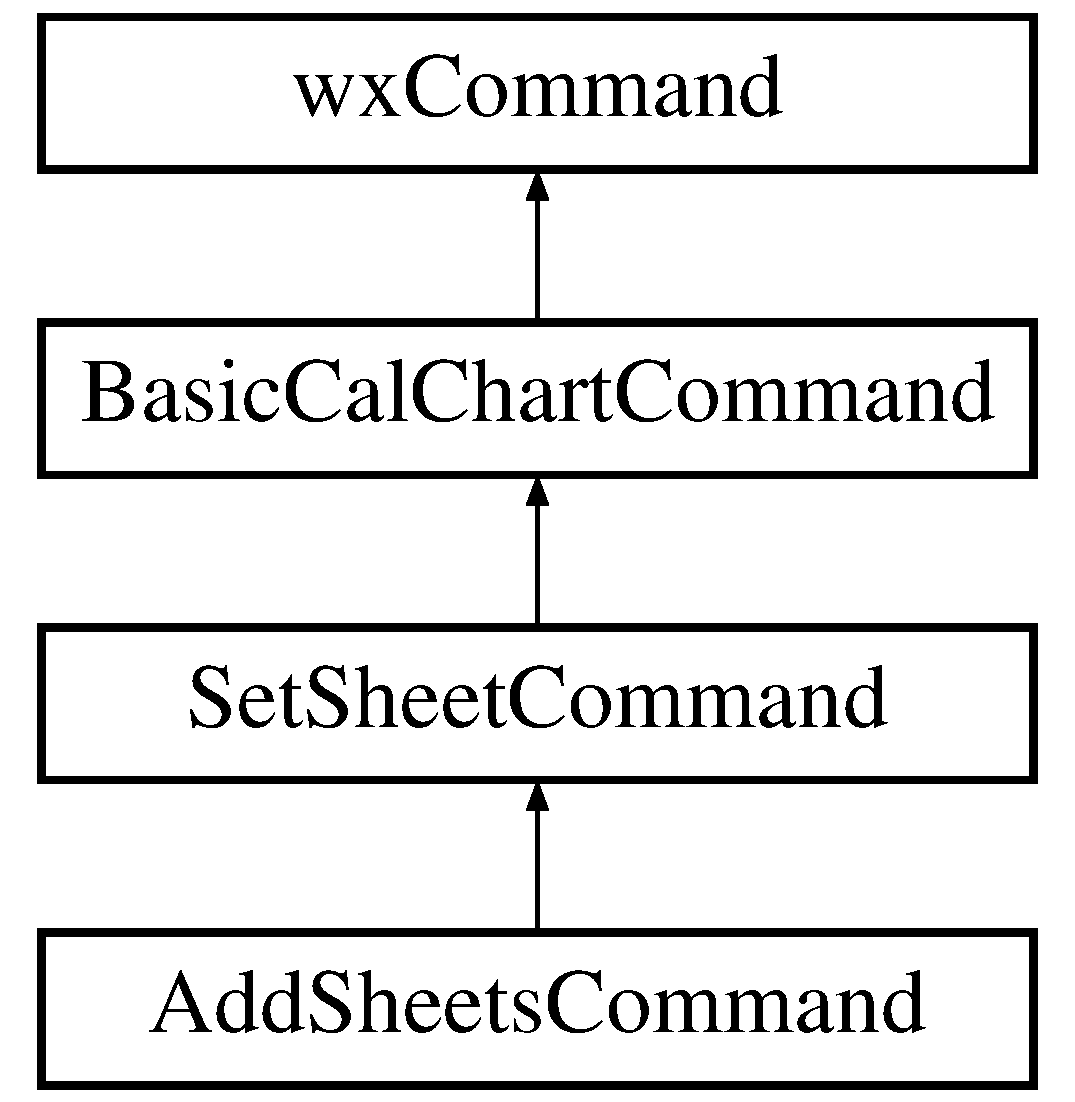
\includegraphics[height=4.000000cm]{a00001}
\end{center}
\end{figure}
\subsection*{Public Member Functions}
\begin{DoxyCompactItemize}
\item 
\hyperlink{a00001_ae67e3a5bfc4cce3030f2956d701333ec}{Add\-Sheets\-Command} (\hyperlink{a00020}{Cal\-Chart\-Doc} \&show, const \hyperlink{a00046_a1a6e11ead9a97c796881971059c56f37}{C\-C\-\_\-show\-::\-C\-C\-\_\-sheet\-\_\-container\-\_\-t} \&sheets, unsigned where)
\item 
virtual \hyperlink{a00001_a2cf09716b4570a170eea345640a586eb}{$\sim$\-Add\-Sheets\-Command} ()
\end{DoxyCompactItemize}
\subsection*{Protected Member Functions}
\begin{DoxyCompactItemize}
\item 
virtual void \hyperlink{a00001_aba46cac1335e29189a9aaf5b50d3f364}{Do\-Action} ()
\end{DoxyCompactItemize}
\subsection*{Protected Attributes}
\begin{DoxyCompactItemize}
\item 
\hyperlink{a00046_a1a6e11ead9a97c796881971059c56f37}{C\-C\-\_\-show\-::\-C\-C\-\_\-sheet\-\_\-container\-\_\-t} \hyperlink{a00001_a1e2bbc755b75b02774e83b5e8c1c27f0}{m\-Sheets}
\item 
const unsigned \hyperlink{a00001_a5456fb7e9af34bf953e0e74628d4165d}{m\-Where}
\end{DoxyCompactItemize}


\subsection{Constructor \& Destructor Documentation}
\hypertarget{a00001_ae67e3a5bfc4cce3030f2956d701333ec}{\index{Add\-Sheets\-Command@{Add\-Sheets\-Command}!Add\-Sheets\-Command@{Add\-Sheets\-Command}}
\index{Add\-Sheets\-Command@{Add\-Sheets\-Command}!AddSheetsCommand@{Add\-Sheets\-Command}}
\subsubsection[{Add\-Sheets\-Command}]{\setlength{\rightskip}{0pt plus 5cm}Add\-Sheets\-Command\-::\-Add\-Sheets\-Command (
\begin{DoxyParamCaption}
\item[{{\bf Cal\-Chart\-Doc} \&}]{show, }
\item[{const {\bf C\-C\-\_\-show\-::\-C\-C\-\_\-sheet\-\_\-container\-\_\-t} \&}]{sheets, }
\item[{unsigned}]{where}
\end{DoxyParamCaption}
)}}\label{a00001_ae67e3a5bfc4cce3030f2956d701333ec}
\hypertarget{a00001_a2cf09716b4570a170eea345640a586eb}{\index{Add\-Sheets\-Command@{Add\-Sheets\-Command}!$\sim$\-Add\-Sheets\-Command@{$\sim$\-Add\-Sheets\-Command}}
\index{$\sim$\-Add\-Sheets\-Command@{$\sim$\-Add\-Sheets\-Command}!AddSheetsCommand@{Add\-Sheets\-Command}}
\subsubsection[{$\sim$\-Add\-Sheets\-Command}]{\setlength{\rightskip}{0pt plus 5cm}Add\-Sheets\-Command\-::$\sim$\-Add\-Sheets\-Command (
\begin{DoxyParamCaption}
{}
\end{DoxyParamCaption}
)\hspace{0.3cm}{\ttfamily [virtual]}}}\label{a00001_a2cf09716b4570a170eea345640a586eb}


\subsection{Member Function Documentation}
\hypertarget{a00001_aba46cac1335e29189a9aaf5b50d3f364}{\index{Add\-Sheets\-Command@{Add\-Sheets\-Command}!Do\-Action@{Do\-Action}}
\index{Do\-Action@{Do\-Action}!AddSheetsCommand@{Add\-Sheets\-Command}}
\subsubsection[{Do\-Action}]{\setlength{\rightskip}{0pt plus 5cm}void Add\-Sheets\-Command\-::\-Do\-Action (
\begin{DoxyParamCaption}
{}
\end{DoxyParamCaption}
)\hspace{0.3cm}{\ttfamily [protected]}, {\ttfamily [virtual]}}}\label{a00001_aba46cac1335e29189a9aaf5b50d3f364}


Reimplemented from \hyperlink{a00134_a027700275d409b94185dfb3aa2d792bb}{Set\-Sheet\-Command}.



\subsection{Member Data Documentation}
\hypertarget{a00001_a1e2bbc755b75b02774e83b5e8c1c27f0}{\index{Add\-Sheets\-Command@{Add\-Sheets\-Command}!m\-Sheets@{m\-Sheets}}
\index{m\-Sheets@{m\-Sheets}!AddSheetsCommand@{Add\-Sheets\-Command}}
\subsubsection[{m\-Sheets}]{\setlength{\rightskip}{0pt plus 5cm}{\bf C\-C\-\_\-show\-::\-C\-C\-\_\-sheet\-\_\-container\-\_\-t} Add\-Sheets\-Command\-::m\-Sheets\hspace{0.3cm}{\ttfamily [protected]}}}\label{a00001_a1e2bbc755b75b02774e83b5e8c1c27f0}
\hypertarget{a00001_a5456fb7e9af34bf953e0e74628d4165d}{\index{Add\-Sheets\-Command@{Add\-Sheets\-Command}!m\-Where@{m\-Where}}
\index{m\-Where@{m\-Where}!AddSheetsCommand@{Add\-Sheets\-Command}}
\subsubsection[{m\-Where}]{\setlength{\rightskip}{0pt plus 5cm}const unsigned Add\-Sheets\-Command\-::m\-Where\hspace{0.3cm}{\ttfamily [protected]}}}\label{a00001_a5456fb7e9af34bf953e0e74628d4165d}


The documentation for this class was generated from the following files\-:\begin{DoxyCompactItemize}
\item 
src/\hyperlink{a00183}{cc\-\_\-command.\-h}\item 
src/\hyperlink{a00182}{cc\-\_\-command.\-cpp}\end{DoxyCompactItemize}

\hypertarget{a00002}{\section{Animation\-:\-:animate\-\_\-info\-\_\-t Struct Reference}
\label{a00002}\index{Animation\-::animate\-\_\-info\-\_\-t@{Animation\-::animate\-\_\-info\-\_\-t}}
}


{\ttfamily \#include $<$animate.\-h$>$}

\subsection*{Public Member Functions}
\begin{DoxyCompactItemize}
\item 
\hyperlink{a00002_a58263c83381a11c44e4908ff38d7f9c5}{animate\-\_\-info\-\_\-t} (bool col, \hyperlink{a00196_a6feaf30c8830fe6fcc0982cb7e9621ab}{Animate\-Dir} dir, float rdir, \hyperlink{a00029}{C\-C\-\_\-coord} pos)
\end{DoxyCompactItemize}
\subsection*{Public Attributes}
\begin{DoxyCompactItemize}
\item 
bool \hyperlink{a00002_af678a7572a0daf31df7f6eec1114c2b7}{m\-Collision}
\item 
\hyperlink{a00196_a6feaf30c8830fe6fcc0982cb7e9621ab}{Animate\-Dir} \hyperlink{a00002_a36f03371754a97ef6b02d325a23fee91}{m\-Direction}
\item 
float \hyperlink{a00002_a57c5464407bead32de395f20f4da671d}{m\-Real\-Direction}
\item 
\hyperlink{a00029}{C\-C\-\_\-coord} \hyperlink{a00002_a85e0fbf440dfb09fcbb34cf453e0b580}{m\-Position}
\end{DoxyCompactItemize}


\subsection{Constructor \& Destructor Documentation}
\hypertarget{a00002_a58263c83381a11c44e4908ff38d7f9c5}{\index{Animation\-::animate\-\_\-info\-\_\-t@{Animation\-::animate\-\_\-info\-\_\-t}!animate\-\_\-info\-\_\-t@{animate\-\_\-info\-\_\-t}}
\index{animate\-\_\-info\-\_\-t@{animate\-\_\-info\-\_\-t}!Animation::animate_info_t@{Animation\-::animate\-\_\-info\-\_\-t}}
\subsubsection[{animate\-\_\-info\-\_\-t}]{\setlength{\rightskip}{0pt plus 5cm}Animation\-::animate\-\_\-info\-\_\-t\-::animate\-\_\-info\-\_\-t (
\begin{DoxyParamCaption}
\item[{bool}]{col, }
\item[{{\bf Animate\-Dir}}]{dir, }
\item[{float}]{rdir, }
\item[{{\bf C\-C\-\_\-coord}}]{pos}
\end{DoxyParamCaption}
)\hspace{0.3cm}{\ttfamily [inline]}}}\label{a00002_a58263c83381a11c44e4908ff38d7f9c5}


\subsection{Member Data Documentation}
\hypertarget{a00002_af678a7572a0daf31df7f6eec1114c2b7}{\index{Animation\-::animate\-\_\-info\-\_\-t@{Animation\-::animate\-\_\-info\-\_\-t}!m\-Collision@{m\-Collision}}
\index{m\-Collision@{m\-Collision}!Animation::animate_info_t@{Animation\-::animate\-\_\-info\-\_\-t}}
\subsubsection[{m\-Collision}]{\setlength{\rightskip}{0pt plus 5cm}bool Animation\-::animate\-\_\-info\-\_\-t\-::m\-Collision}}\label{a00002_af678a7572a0daf31df7f6eec1114c2b7}
\hypertarget{a00002_a36f03371754a97ef6b02d325a23fee91}{\index{Animation\-::animate\-\_\-info\-\_\-t@{Animation\-::animate\-\_\-info\-\_\-t}!m\-Direction@{m\-Direction}}
\index{m\-Direction@{m\-Direction}!Animation::animate_info_t@{Animation\-::animate\-\_\-info\-\_\-t}}
\subsubsection[{m\-Direction}]{\setlength{\rightskip}{0pt plus 5cm}{\bf Animate\-Dir} Animation\-::animate\-\_\-info\-\_\-t\-::m\-Direction}}\label{a00002_a36f03371754a97ef6b02d325a23fee91}
\hypertarget{a00002_a85e0fbf440dfb09fcbb34cf453e0b580}{\index{Animation\-::animate\-\_\-info\-\_\-t@{Animation\-::animate\-\_\-info\-\_\-t}!m\-Position@{m\-Position}}
\index{m\-Position@{m\-Position}!Animation::animate_info_t@{Animation\-::animate\-\_\-info\-\_\-t}}
\subsubsection[{m\-Position}]{\setlength{\rightskip}{0pt plus 5cm}{\bf C\-C\-\_\-coord} Animation\-::animate\-\_\-info\-\_\-t\-::m\-Position}}\label{a00002_a85e0fbf440dfb09fcbb34cf453e0b580}
\hypertarget{a00002_a57c5464407bead32de395f20f4da671d}{\index{Animation\-::animate\-\_\-info\-\_\-t@{Animation\-::animate\-\_\-info\-\_\-t}!m\-Real\-Direction@{m\-Real\-Direction}}
\index{m\-Real\-Direction@{m\-Real\-Direction}!Animation::animate_info_t@{Animation\-::animate\-\_\-info\-\_\-t}}
\subsubsection[{m\-Real\-Direction}]{\setlength{\rightskip}{0pt plus 5cm}float Animation\-::animate\-\_\-info\-\_\-t\-::m\-Real\-Direction}}\label{a00002_a57c5464407bead32de395f20f4da671d}


The documentation for this struct was generated from the following file\-:\begin{DoxyCompactItemize}
\item 
src/core/\hyperlink{a00195}{animate.\-h}\end{DoxyCompactItemize}

\hypertarget{a00003}{\section{Animate\-Command Class Reference}
\label{a00003}\index{Animate\-Command@{Animate\-Command}}
}


{\ttfamily \#include $<$animatecommand.\-h$>$}

Inheritance diagram for Animate\-Command\-:\begin{figure}[H]
\begin{center}
\leavevmode
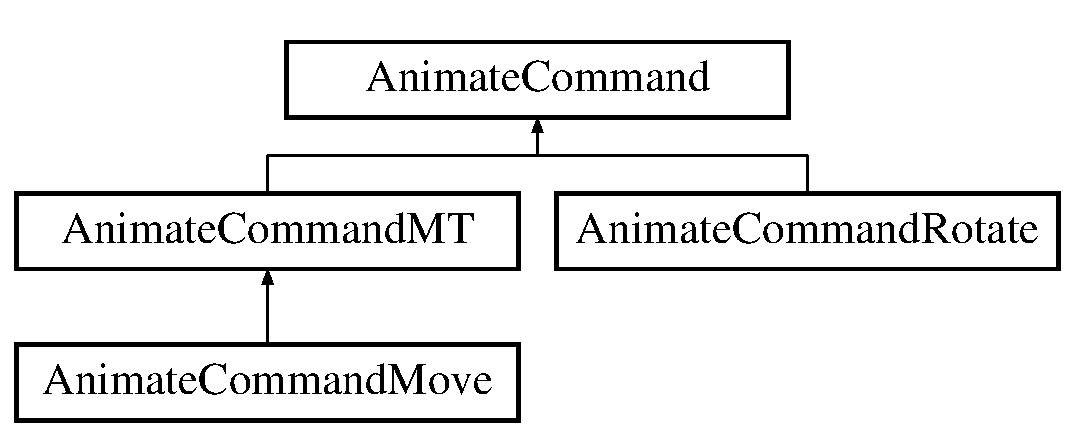
\includegraphics[height=3.000000cm]{a00003}
\end{center}
\end{figure}
\subsection*{Public Member Functions}
\begin{DoxyCompactItemize}
\item 
\hyperlink{a00003_aebfee0fad0d8e0fb34b5aa51b4798acc}{Animate\-Command} (unsigned beats)
\item 
virtual \hyperlink{a00003_ac5e46568837cf7ba139dd67df6a2f431}{$\sim$\-Animate\-Command} ()
\item 
virtual bool \hyperlink{a00003_ab69372e28870271550dd8c8a54da02ee}{Begin} (\hyperlink{a00196_a91212e6bb797b2b440819b6a9a86f702}{Animate\-Point} \&pt)
\item 
virtual bool \hyperlink{a00003_ae5dfaac6e8cf870a688a8e3161672b4e}{End} (\hyperlink{a00196_a91212e6bb797b2b440819b6a9a86f702}{Animate\-Point} \&pt)
\item 
virtual bool \hyperlink{a00003_a80bcd30c221c961d87049dee4d9eff5e}{Next\-Beat} (\hyperlink{a00196_a91212e6bb797b2b440819b6a9a86f702}{Animate\-Point} \&pt)
\item 
virtual bool \hyperlink{a00003_aafde773d0e8074306eed850c91c7f207}{Prev\-Beat} (\hyperlink{a00196_a91212e6bb797b2b440819b6a9a86f702}{Animate\-Point} \&pt)
\item 
virtual void \hyperlink{a00003_af8a485b986aacf649f41c81e4d6eeed9}{Apply\-Forward} (\hyperlink{a00196_a91212e6bb797b2b440819b6a9a86f702}{Animate\-Point} \&pt)
\item 
virtual void \hyperlink{a00003_a969de0c473c2ca7d2f3b9ea8748fffb7}{Apply\-Backward} (\hyperlink{a00196_a91212e6bb797b2b440819b6a9a86f702}{Animate\-Point} \&pt)
\item 
virtual \hyperlink{a00196_a6feaf30c8830fe6fcc0982cb7e9621ab}{Animate\-Dir} \hyperlink{a00003_ada84c0464a78c98eb9b24e64f1ea2e36}{Direction} () const =0
\item 
virtual float \hyperlink{a00003_a23b1c7a078df01cb31adaad24d29c27d}{Real\-Direction} () const =0
\item 
virtual float \hyperlink{a00003_af131cd1634440010576620cd6ad8a2c1}{Motion\-Direction} () const 
\item 
virtual void \hyperlink{a00003_ace20ca13c14bf94e13404df0ef825da8}{Clip\-Beats} (unsigned beats)
\item 
virtual unsigned \hyperlink{a00003_af182790906aec055af4e35f3b962f89a}{Num\-Beats} () const 
\item 
virtual \hyperlink{a00196_a56c9857b8353188d8e6823c408ba71ad}{Marching\-Style} \hyperlink{a00003_a245f81fa1ee5a43bbaaa364107b13c1e}{Step\-Style} ()
\item 
virtual \hyperlink{a00031}{C\-C\-\_\-\-Draw\-Command} \hyperlink{a00003_a34d8e8a89c11f7ef6d1e2346db77d462}{Gen\-C\-C\-\_\-\-Draw\-Command} (const \hyperlink{a00196_a91212e6bb797b2b440819b6a9a86f702}{Animate\-Point} \&pt, const \hyperlink{a00029}{C\-C\-\_\-coord} \&offset) const 
\end{DoxyCompactItemize}
\subsection*{Protected Attributes}
\begin{DoxyCompactItemize}
\item 
unsigned \hyperlink{a00003_a6bc20b1356872227a55ba176ec85fa1f}{m\-Num\-Beats}
\item 
unsigned \hyperlink{a00003_af6ac5dcbcef33378b6729eec09f9dbc4}{m\-Beat}
\end{DoxyCompactItemize}


\subsection{Constructor \& Destructor Documentation}
\hypertarget{a00003_aebfee0fad0d8e0fb34b5aa51b4798acc}{\index{Animate\-Command@{Animate\-Command}!Animate\-Command@{Animate\-Command}}
\index{Animate\-Command@{Animate\-Command}!AnimateCommand@{Animate\-Command}}
\subsubsection[{Animate\-Command}]{\setlength{\rightskip}{0pt plus 5cm}Animate\-Command\-::\-Animate\-Command (
\begin{DoxyParamCaption}
\item[{unsigned}]{beats}
\end{DoxyParamCaption}
)}}\label{a00003_aebfee0fad0d8e0fb34b5aa51b4798acc}
\hypertarget{a00003_ac5e46568837cf7ba139dd67df6a2f431}{\index{Animate\-Command@{Animate\-Command}!$\sim$\-Animate\-Command@{$\sim$\-Animate\-Command}}
\index{$\sim$\-Animate\-Command@{$\sim$\-Animate\-Command}!AnimateCommand@{Animate\-Command}}
\subsubsection[{$\sim$\-Animate\-Command}]{\setlength{\rightskip}{0pt plus 5cm}Animate\-Command\-::$\sim$\-Animate\-Command (
\begin{DoxyParamCaption}
{}
\end{DoxyParamCaption}
)\hspace{0.3cm}{\ttfamily [virtual]}}}\label{a00003_ac5e46568837cf7ba139dd67df6a2f431}


\subsection{Member Function Documentation}
\hypertarget{a00003_a969de0c473c2ca7d2f3b9ea8748fffb7}{\index{Animate\-Command@{Animate\-Command}!Apply\-Backward@{Apply\-Backward}}
\index{Apply\-Backward@{Apply\-Backward}!AnimateCommand@{Animate\-Command}}
\subsubsection[{Apply\-Backward}]{\setlength{\rightskip}{0pt plus 5cm}void Animate\-Command\-::\-Apply\-Backward (
\begin{DoxyParamCaption}
\item[{{\bf Animate\-Point} \&}]{pt}
\end{DoxyParamCaption}
)\hspace{0.3cm}{\ttfamily [virtual]}}}\label{a00003_a969de0c473c2ca7d2f3b9ea8748fffb7}


Reimplemented in \hyperlink{a00006_af8f47135c6190dc9363a4d7705ad443a}{Animate\-Command\-Rotate}, and \hyperlink{a00004_a04bbf87bd1472184d5129d387b669db5}{Animate\-Command\-Move}.

\hypertarget{a00003_af8a485b986aacf649f41c81e4d6eeed9}{\index{Animate\-Command@{Animate\-Command}!Apply\-Forward@{Apply\-Forward}}
\index{Apply\-Forward@{Apply\-Forward}!AnimateCommand@{Animate\-Command}}
\subsubsection[{Apply\-Forward}]{\setlength{\rightskip}{0pt plus 5cm}void Animate\-Command\-::\-Apply\-Forward (
\begin{DoxyParamCaption}
\item[{{\bf Animate\-Point} \&}]{pt}
\end{DoxyParamCaption}
)\hspace{0.3cm}{\ttfamily [virtual]}}}\label{a00003_af8a485b986aacf649f41c81e4d6eeed9}


Reimplemented in \hyperlink{a00006_a0ef1ae2cc3ca46a734b231bb38347f79}{Animate\-Command\-Rotate}, and \hyperlink{a00004_aca53b3ec977640ccce4765a5001d211b}{Animate\-Command\-Move}.

\hypertarget{a00003_ab69372e28870271550dd8c8a54da02ee}{\index{Animate\-Command@{Animate\-Command}!Begin@{Begin}}
\index{Begin@{Begin}!AnimateCommand@{Animate\-Command}}
\subsubsection[{Begin}]{\setlength{\rightskip}{0pt plus 5cm}bool Animate\-Command\-::\-Begin (
\begin{DoxyParamCaption}
\item[{{\bf Animate\-Point} \&}]{pt}
\end{DoxyParamCaption}
)\hspace{0.3cm}{\ttfamily [virtual]}}}\label{a00003_ab69372e28870271550dd8c8a54da02ee}
\hypertarget{a00003_ace20ca13c14bf94e13404df0ef825da8}{\index{Animate\-Command@{Animate\-Command}!Clip\-Beats@{Clip\-Beats}}
\index{Clip\-Beats@{Clip\-Beats}!AnimateCommand@{Animate\-Command}}
\subsubsection[{Clip\-Beats}]{\setlength{\rightskip}{0pt plus 5cm}void Animate\-Command\-::\-Clip\-Beats (
\begin{DoxyParamCaption}
\item[{unsigned}]{beats}
\end{DoxyParamCaption}
)\hspace{0.3cm}{\ttfamily [virtual]}}}\label{a00003_ace20ca13c14bf94e13404df0ef825da8}


Reimplemented in \hyperlink{a00006_a865113f57c577626241256ab35981834}{Animate\-Command\-Rotate}, and \hyperlink{a00004_aecf325aaf810ee9fe14e39f86812b504}{Animate\-Command\-Move}.

\hypertarget{a00003_ada84c0464a78c98eb9b24e64f1ea2e36}{\index{Animate\-Command@{Animate\-Command}!Direction@{Direction}}
\index{Direction@{Direction}!AnimateCommand@{Animate\-Command}}
\subsubsection[{Direction}]{\setlength{\rightskip}{0pt plus 5cm}virtual {\bf Animate\-Dir} Animate\-Command\-::\-Direction (
\begin{DoxyParamCaption}
{}
\end{DoxyParamCaption}
) const\hspace{0.3cm}{\ttfamily [pure virtual]}}}\label{a00003_ada84c0464a78c98eb9b24e64f1ea2e36}


Implemented in \hyperlink{a00006_ad534024d6bd630dfc0cde5e07649094a}{Animate\-Command\-Rotate}, and \hyperlink{a00005_a0f746d2dce20a8159f4534e555079501}{Animate\-Command\-M\-T}.

\hypertarget{a00003_ae5dfaac6e8cf870a688a8e3161672b4e}{\index{Animate\-Command@{Animate\-Command}!End@{End}}
\index{End@{End}!AnimateCommand@{Animate\-Command}}
\subsubsection[{End}]{\setlength{\rightskip}{0pt plus 5cm}bool Animate\-Command\-::\-End (
\begin{DoxyParamCaption}
\item[{{\bf Animate\-Point} \&}]{pt}
\end{DoxyParamCaption}
)\hspace{0.3cm}{\ttfamily [virtual]}}}\label{a00003_ae5dfaac6e8cf870a688a8e3161672b4e}
\hypertarget{a00003_a34d8e8a89c11f7ef6d1e2346db77d462}{\index{Animate\-Command@{Animate\-Command}!Gen\-C\-C\-\_\-\-Draw\-Command@{Gen\-C\-C\-\_\-\-Draw\-Command}}
\index{Gen\-C\-C\-\_\-\-Draw\-Command@{Gen\-C\-C\-\_\-\-Draw\-Command}!AnimateCommand@{Animate\-Command}}
\subsubsection[{Gen\-C\-C\-\_\-\-Draw\-Command}]{\setlength{\rightskip}{0pt plus 5cm}virtual {\bf C\-C\-\_\-\-Draw\-Command} Animate\-Command\-::\-Gen\-C\-C\-\_\-\-Draw\-Command (
\begin{DoxyParamCaption}
\item[{const {\bf Animate\-Point} \&}]{pt, }
\item[{const {\bf C\-C\-\_\-coord} \&}]{offset}
\end{DoxyParamCaption}
) const\hspace{0.3cm}{\ttfamily [inline]}, {\ttfamily [virtual]}}}\label{a00003_a34d8e8a89c11f7ef6d1e2346db77d462}


Reimplemented in \hyperlink{a00006_a999e00a33481237a53af76481913d83f}{Animate\-Command\-Rotate}, and \hyperlink{a00004_aaa097d316852a0a16ec6d71942ecef4b}{Animate\-Command\-Move}.

\hypertarget{a00003_af131cd1634440010576620cd6ad8a2c1}{\index{Animate\-Command@{Animate\-Command}!Motion\-Direction@{Motion\-Direction}}
\index{Motion\-Direction@{Motion\-Direction}!AnimateCommand@{Animate\-Command}}
\subsubsection[{Motion\-Direction}]{\setlength{\rightskip}{0pt plus 5cm}float Animate\-Command\-::\-Motion\-Direction (
\begin{DoxyParamCaption}
{}
\end{DoxyParamCaption}
) const\hspace{0.3cm}{\ttfamily [virtual]}}}\label{a00003_af131cd1634440010576620cd6ad8a2c1}


Reimplemented in \hyperlink{a00004_a76e50136a8930c4a0020371c45f447ab}{Animate\-Command\-Move}.

\hypertarget{a00003_a80bcd30c221c961d87049dee4d9eff5e}{\index{Animate\-Command@{Animate\-Command}!Next\-Beat@{Next\-Beat}}
\index{Next\-Beat@{Next\-Beat}!AnimateCommand@{Animate\-Command}}
\subsubsection[{Next\-Beat}]{\setlength{\rightskip}{0pt plus 5cm}bool Animate\-Command\-::\-Next\-Beat (
\begin{DoxyParamCaption}
\item[{{\bf Animate\-Point} \&}]{pt}
\end{DoxyParamCaption}
)\hspace{0.3cm}{\ttfamily [virtual]}}}\label{a00003_a80bcd30c221c961d87049dee4d9eff5e}


Reimplemented in \hyperlink{a00006_a5d1ee680f19374391a6fbccdcd6b6bb7}{Animate\-Command\-Rotate}, and \hyperlink{a00004_aae66871bc335cfc08f1d843b0c070bd8}{Animate\-Command\-Move}.

\hypertarget{a00003_af182790906aec055af4e35f3b962f89a}{\index{Animate\-Command@{Animate\-Command}!Num\-Beats@{Num\-Beats}}
\index{Num\-Beats@{Num\-Beats}!AnimateCommand@{Animate\-Command}}
\subsubsection[{Num\-Beats}]{\setlength{\rightskip}{0pt plus 5cm}virtual unsigned Animate\-Command\-::\-Num\-Beats (
\begin{DoxyParamCaption}
{}
\end{DoxyParamCaption}
) const\hspace{0.3cm}{\ttfamily [inline]}, {\ttfamily [virtual]}}}\label{a00003_af182790906aec055af4e35f3b962f89a}
\hypertarget{a00003_aafde773d0e8074306eed850c91c7f207}{\index{Animate\-Command@{Animate\-Command}!Prev\-Beat@{Prev\-Beat}}
\index{Prev\-Beat@{Prev\-Beat}!AnimateCommand@{Animate\-Command}}
\subsubsection[{Prev\-Beat}]{\setlength{\rightskip}{0pt plus 5cm}bool Animate\-Command\-::\-Prev\-Beat (
\begin{DoxyParamCaption}
\item[{{\bf Animate\-Point} \&}]{pt}
\end{DoxyParamCaption}
)\hspace{0.3cm}{\ttfamily [virtual]}}}\label{a00003_aafde773d0e8074306eed850c91c7f207}


Reimplemented in \hyperlink{a00006_a179b843d1c400020f0fbb106a09c38e5}{Animate\-Command\-Rotate}, and \hyperlink{a00004_a0fc987b85dc91d4dc45663584d59f3b6}{Animate\-Command\-Move}.

\hypertarget{a00003_a23b1c7a078df01cb31adaad24d29c27d}{\index{Animate\-Command@{Animate\-Command}!Real\-Direction@{Real\-Direction}}
\index{Real\-Direction@{Real\-Direction}!AnimateCommand@{Animate\-Command}}
\subsubsection[{Real\-Direction}]{\setlength{\rightskip}{0pt plus 5cm}virtual float Animate\-Command\-::\-Real\-Direction (
\begin{DoxyParamCaption}
{}
\end{DoxyParamCaption}
) const\hspace{0.3cm}{\ttfamily [pure virtual]}}}\label{a00003_a23b1c7a078df01cb31adaad24d29c27d}


Implemented in \hyperlink{a00006_afd366a7d56e16f296a80faab4ffe4972}{Animate\-Command\-Rotate}, and \hyperlink{a00005_a09339d867d2968b5db48faf0f9cc4891}{Animate\-Command\-M\-T}.

\hypertarget{a00003_a245f81fa1ee5a43bbaaa364107b13c1e}{\index{Animate\-Command@{Animate\-Command}!Step\-Style@{Step\-Style}}
\index{Step\-Style@{Step\-Style}!AnimateCommand@{Animate\-Command}}
\subsubsection[{Step\-Style}]{\setlength{\rightskip}{0pt plus 5cm}virtual {\bf Marching\-Style} Animate\-Command\-::\-Step\-Style (
\begin{DoxyParamCaption}
{}
\end{DoxyParamCaption}
)\hspace{0.3cm}{\ttfamily [inline]}, {\ttfamily [virtual]}}}\label{a00003_a245f81fa1ee5a43bbaaa364107b13c1e}


\subsection{Member Data Documentation}
\hypertarget{a00003_af6ac5dcbcef33378b6729eec09f9dbc4}{\index{Animate\-Command@{Animate\-Command}!m\-Beat@{m\-Beat}}
\index{m\-Beat@{m\-Beat}!AnimateCommand@{Animate\-Command}}
\subsubsection[{m\-Beat}]{\setlength{\rightskip}{0pt plus 5cm}unsigned Animate\-Command\-::m\-Beat\hspace{0.3cm}{\ttfamily [protected]}}}\label{a00003_af6ac5dcbcef33378b6729eec09f9dbc4}
\hypertarget{a00003_a6bc20b1356872227a55ba176ec85fa1f}{\index{Animate\-Command@{Animate\-Command}!m\-Num\-Beats@{m\-Num\-Beats}}
\index{m\-Num\-Beats@{m\-Num\-Beats}!AnimateCommand@{Animate\-Command}}
\subsubsection[{m\-Num\-Beats}]{\setlength{\rightskip}{0pt plus 5cm}unsigned Animate\-Command\-::m\-Num\-Beats\hspace{0.3cm}{\ttfamily [protected]}}}\label{a00003_a6bc20b1356872227a55ba176ec85fa1f}


The documentation for this class was generated from the following files\-:\begin{DoxyCompactItemize}
\item 
src/core/\hyperlink{a00198}{animatecommand.\-h}\item 
src/core/\hyperlink{a00197}{animatecommand.\-cpp}\end{DoxyCompactItemize}

\hypertarget{a00004}{\section{Animate\-Command\-Move Class Reference}
\label{a00004}\index{Animate\-Command\-Move@{Animate\-Command\-Move}}
}


{\ttfamily \#include $<$animatecommand.\-h$>$}

Inheritance diagram for Animate\-Command\-Move\-:\begin{figure}[H]
\begin{center}
\leavevmode
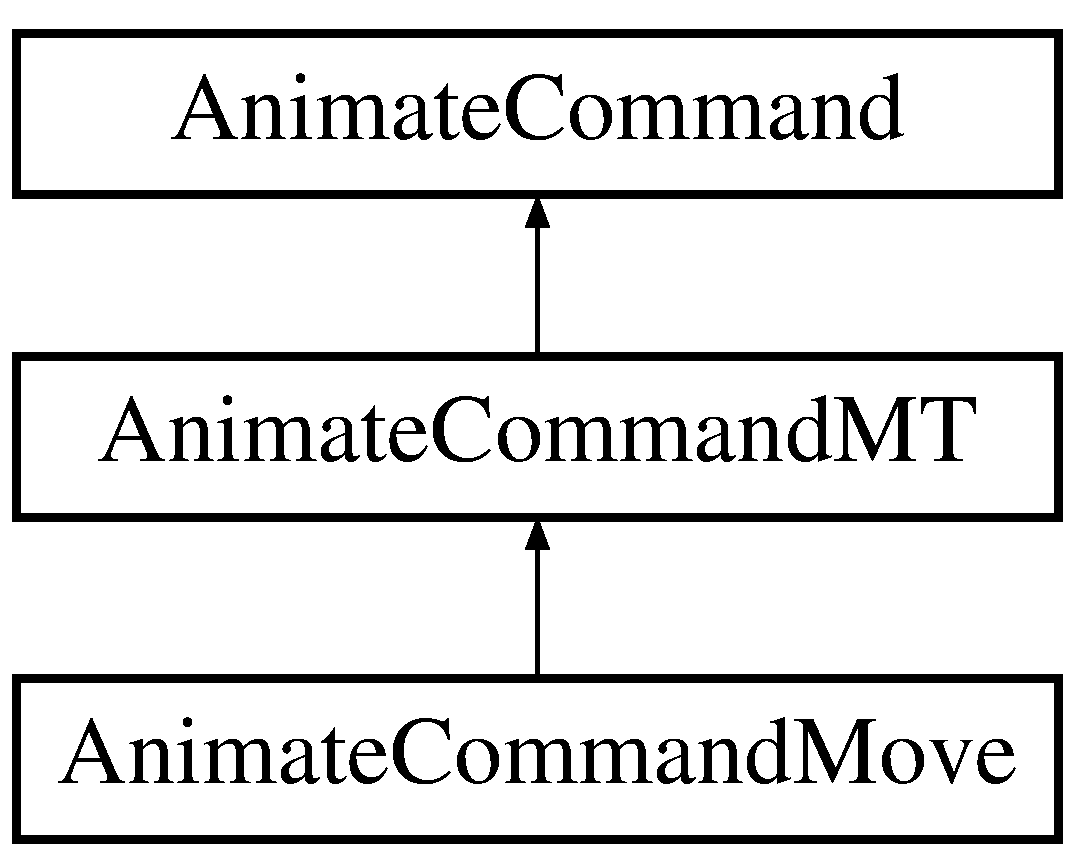
\includegraphics[height=3.000000cm]{a00004}
\end{center}
\end{figure}
\subsection*{Public Member Functions}
\begin{DoxyCompactItemize}
\item 
\hyperlink{a00004_ab9ed9fbe25a224296fdd84996654751e}{Animate\-Command\-Move} (unsigned beats, \hyperlink{a00029}{C\-C\-\_\-coord} movement)
\item 
\hyperlink{a00004_aecd0d0f177c8e4f477b4f7c598317f1c}{Animate\-Command\-Move} (unsigned beats, \hyperlink{a00029}{C\-C\-\_\-coord} movement, float direction)
\item 
virtual \hyperlink{a00004_a76137e78b51f9f066ba1d451f65bec17}{$\sim$\-Animate\-Command\-Move} ()
\item 
virtual bool \hyperlink{a00004_aae66871bc335cfc08f1d843b0c070bd8}{Next\-Beat} (\hyperlink{a00196_a91212e6bb797b2b440819b6a9a86f702}{Animate\-Point} \&pt)
\item 
virtual bool \hyperlink{a00004_a0fc987b85dc91d4dc45663584d59f3b6}{Prev\-Beat} (\hyperlink{a00196_a91212e6bb797b2b440819b6a9a86f702}{Animate\-Point} \&pt)
\item 
virtual void \hyperlink{a00004_aca53b3ec977640ccce4765a5001d211b}{Apply\-Forward} (\hyperlink{a00196_a91212e6bb797b2b440819b6a9a86f702}{Animate\-Point} \&pt)
\item 
virtual void \hyperlink{a00004_a04bbf87bd1472184d5129d387b669db5}{Apply\-Backward} (\hyperlink{a00196_a91212e6bb797b2b440819b6a9a86f702}{Animate\-Point} \&pt)
\item 
virtual float \hyperlink{a00004_a76e50136a8930c4a0020371c45f447ab}{Motion\-Direction} () const 
\item 
virtual void \hyperlink{a00004_aecf325aaf810ee9fe14e39f86812b504}{Clip\-Beats} (unsigned beats)
\item 
virtual \hyperlink{a00031}{C\-C\-\_\-\-Draw\-Command} \hyperlink{a00004_aaa097d316852a0a16ec6d71942ecef4b}{Gen\-C\-C\-\_\-\-Draw\-Command} (const \hyperlink{a00196_a91212e6bb797b2b440819b6a9a86f702}{Animate\-Point} \&pt, const \hyperlink{a00029}{C\-C\-\_\-coord} \&offset) const 
\end{DoxyCompactItemize}
\subsection*{Private Attributes}
\begin{DoxyCompactItemize}
\item 
\hyperlink{a00029}{C\-C\-\_\-coord} \hyperlink{a00004_a73fff2220ae93d1539df36d94d5e6b83}{m\-Vector}
\end{DoxyCompactItemize}
\subsection*{Additional Inherited Members}


\subsection{Constructor \& Destructor Documentation}
\hypertarget{a00004_ab9ed9fbe25a224296fdd84996654751e}{\index{Animate\-Command\-Move@{Animate\-Command\-Move}!Animate\-Command\-Move@{Animate\-Command\-Move}}
\index{Animate\-Command\-Move@{Animate\-Command\-Move}!AnimateCommandMove@{Animate\-Command\-Move}}
\subsubsection[{Animate\-Command\-Move}]{\setlength{\rightskip}{0pt plus 5cm}Animate\-Command\-Move\-::\-Animate\-Command\-Move (
\begin{DoxyParamCaption}
\item[{unsigned}]{beats, }
\item[{{\bf C\-C\-\_\-coord}}]{movement}
\end{DoxyParamCaption}
)}}\label{a00004_ab9ed9fbe25a224296fdd84996654751e}
\hypertarget{a00004_aecd0d0f177c8e4f477b4f7c598317f1c}{\index{Animate\-Command\-Move@{Animate\-Command\-Move}!Animate\-Command\-Move@{Animate\-Command\-Move}}
\index{Animate\-Command\-Move@{Animate\-Command\-Move}!AnimateCommandMove@{Animate\-Command\-Move}}
\subsubsection[{Animate\-Command\-Move}]{\setlength{\rightskip}{0pt plus 5cm}Animate\-Command\-Move\-::\-Animate\-Command\-Move (
\begin{DoxyParamCaption}
\item[{unsigned}]{beats, }
\item[{{\bf C\-C\-\_\-coord}}]{movement, }
\item[{float}]{direction}
\end{DoxyParamCaption}
)}}\label{a00004_aecd0d0f177c8e4f477b4f7c598317f1c}
\hypertarget{a00004_a76137e78b51f9f066ba1d451f65bec17}{\index{Animate\-Command\-Move@{Animate\-Command\-Move}!$\sim$\-Animate\-Command\-Move@{$\sim$\-Animate\-Command\-Move}}
\index{$\sim$\-Animate\-Command\-Move@{$\sim$\-Animate\-Command\-Move}!AnimateCommandMove@{Animate\-Command\-Move}}
\subsubsection[{$\sim$\-Animate\-Command\-Move}]{\setlength{\rightskip}{0pt plus 5cm}virtual Animate\-Command\-Move\-::$\sim$\-Animate\-Command\-Move (
\begin{DoxyParamCaption}
{}
\end{DoxyParamCaption}
)\hspace{0.3cm}{\ttfamily [inline]}, {\ttfamily [virtual]}}}\label{a00004_a76137e78b51f9f066ba1d451f65bec17}


\subsection{Member Function Documentation}
\hypertarget{a00004_a04bbf87bd1472184d5129d387b669db5}{\index{Animate\-Command\-Move@{Animate\-Command\-Move}!Apply\-Backward@{Apply\-Backward}}
\index{Apply\-Backward@{Apply\-Backward}!AnimateCommandMove@{Animate\-Command\-Move}}
\subsubsection[{Apply\-Backward}]{\setlength{\rightskip}{0pt plus 5cm}void Animate\-Command\-Move\-::\-Apply\-Backward (
\begin{DoxyParamCaption}
\item[{{\bf Animate\-Point} \&}]{pt}
\end{DoxyParamCaption}
)\hspace{0.3cm}{\ttfamily [virtual]}}}\label{a00004_a04bbf87bd1472184d5129d387b669db5}


Reimplemented from \hyperlink{a00003_a969de0c473c2ca7d2f3b9ea8748fffb7}{Animate\-Command}.

\hypertarget{a00004_aca53b3ec977640ccce4765a5001d211b}{\index{Animate\-Command\-Move@{Animate\-Command\-Move}!Apply\-Forward@{Apply\-Forward}}
\index{Apply\-Forward@{Apply\-Forward}!AnimateCommandMove@{Animate\-Command\-Move}}
\subsubsection[{Apply\-Forward}]{\setlength{\rightskip}{0pt plus 5cm}void Animate\-Command\-Move\-::\-Apply\-Forward (
\begin{DoxyParamCaption}
\item[{{\bf Animate\-Point} \&}]{pt}
\end{DoxyParamCaption}
)\hspace{0.3cm}{\ttfamily [virtual]}}}\label{a00004_aca53b3ec977640ccce4765a5001d211b}


Reimplemented from \hyperlink{a00003_af8a485b986aacf649f41c81e4d6eeed9}{Animate\-Command}.

\hypertarget{a00004_aecf325aaf810ee9fe14e39f86812b504}{\index{Animate\-Command\-Move@{Animate\-Command\-Move}!Clip\-Beats@{Clip\-Beats}}
\index{Clip\-Beats@{Clip\-Beats}!AnimateCommandMove@{Animate\-Command\-Move}}
\subsubsection[{Clip\-Beats}]{\setlength{\rightskip}{0pt plus 5cm}void Animate\-Command\-Move\-::\-Clip\-Beats (
\begin{DoxyParamCaption}
\item[{unsigned}]{beats}
\end{DoxyParamCaption}
)\hspace{0.3cm}{\ttfamily [virtual]}}}\label{a00004_aecf325aaf810ee9fe14e39f86812b504}


Reimplemented from \hyperlink{a00003_ace20ca13c14bf94e13404df0ef825da8}{Animate\-Command}.

\hypertarget{a00004_aaa097d316852a0a16ec6d71942ecef4b}{\index{Animate\-Command\-Move@{Animate\-Command\-Move}!Gen\-C\-C\-\_\-\-Draw\-Command@{Gen\-C\-C\-\_\-\-Draw\-Command}}
\index{Gen\-C\-C\-\_\-\-Draw\-Command@{Gen\-C\-C\-\_\-\-Draw\-Command}!AnimateCommandMove@{Animate\-Command\-Move}}
\subsubsection[{Gen\-C\-C\-\_\-\-Draw\-Command}]{\setlength{\rightskip}{0pt plus 5cm}{\bf C\-C\-\_\-\-Draw\-Command} Animate\-Command\-Move\-::\-Gen\-C\-C\-\_\-\-Draw\-Command (
\begin{DoxyParamCaption}
\item[{const {\bf Animate\-Point} \&}]{pt, }
\item[{const {\bf C\-C\-\_\-coord} \&}]{offset}
\end{DoxyParamCaption}
) const\hspace{0.3cm}{\ttfamily [virtual]}}}\label{a00004_aaa097d316852a0a16ec6d71942ecef4b}


Reimplemented from \hyperlink{a00003_a34d8e8a89c11f7ef6d1e2346db77d462}{Animate\-Command}.

\hypertarget{a00004_a76e50136a8930c4a0020371c45f447ab}{\index{Animate\-Command\-Move@{Animate\-Command\-Move}!Motion\-Direction@{Motion\-Direction}}
\index{Motion\-Direction@{Motion\-Direction}!AnimateCommandMove@{Animate\-Command\-Move}}
\subsubsection[{Motion\-Direction}]{\setlength{\rightskip}{0pt plus 5cm}float Animate\-Command\-Move\-::\-Motion\-Direction (
\begin{DoxyParamCaption}
{}
\end{DoxyParamCaption}
) const\hspace{0.3cm}{\ttfamily [virtual]}}}\label{a00004_a76e50136a8930c4a0020371c45f447ab}


Reimplemented from \hyperlink{a00003_af131cd1634440010576620cd6ad8a2c1}{Animate\-Command}.

\hypertarget{a00004_aae66871bc335cfc08f1d843b0c070bd8}{\index{Animate\-Command\-Move@{Animate\-Command\-Move}!Next\-Beat@{Next\-Beat}}
\index{Next\-Beat@{Next\-Beat}!AnimateCommandMove@{Animate\-Command\-Move}}
\subsubsection[{Next\-Beat}]{\setlength{\rightskip}{0pt plus 5cm}bool Animate\-Command\-Move\-::\-Next\-Beat (
\begin{DoxyParamCaption}
\item[{{\bf Animate\-Point} \&}]{pt}
\end{DoxyParamCaption}
)\hspace{0.3cm}{\ttfamily [virtual]}}}\label{a00004_aae66871bc335cfc08f1d843b0c070bd8}


Reimplemented from \hyperlink{a00003_a80bcd30c221c961d87049dee4d9eff5e}{Animate\-Command}.

\hypertarget{a00004_a0fc987b85dc91d4dc45663584d59f3b6}{\index{Animate\-Command\-Move@{Animate\-Command\-Move}!Prev\-Beat@{Prev\-Beat}}
\index{Prev\-Beat@{Prev\-Beat}!AnimateCommandMove@{Animate\-Command\-Move}}
\subsubsection[{Prev\-Beat}]{\setlength{\rightskip}{0pt plus 5cm}bool Animate\-Command\-Move\-::\-Prev\-Beat (
\begin{DoxyParamCaption}
\item[{{\bf Animate\-Point} \&}]{pt}
\end{DoxyParamCaption}
)\hspace{0.3cm}{\ttfamily [virtual]}}}\label{a00004_a0fc987b85dc91d4dc45663584d59f3b6}


Reimplemented from \hyperlink{a00003_aafde773d0e8074306eed850c91c7f207}{Animate\-Command}.



\subsection{Member Data Documentation}
\hypertarget{a00004_a73fff2220ae93d1539df36d94d5e6b83}{\index{Animate\-Command\-Move@{Animate\-Command\-Move}!m\-Vector@{m\-Vector}}
\index{m\-Vector@{m\-Vector}!AnimateCommandMove@{Animate\-Command\-Move}}
\subsubsection[{m\-Vector}]{\setlength{\rightskip}{0pt plus 5cm}{\bf C\-C\-\_\-coord} Animate\-Command\-Move\-::m\-Vector\hspace{0.3cm}{\ttfamily [private]}}}\label{a00004_a73fff2220ae93d1539df36d94d5e6b83}


The documentation for this class was generated from the following files\-:\begin{DoxyCompactItemize}
\item 
src/core/\hyperlink{a00198}{animatecommand.\-h}\item 
src/core/\hyperlink{a00197}{animatecommand.\-cpp}\end{DoxyCompactItemize}

\hypertarget{a00005}{\section{Animate\-Command\-M\-T Class Reference}
\label{a00005}\index{Animate\-Command\-M\-T@{Animate\-Command\-M\-T}}
}


{\ttfamily \#include $<$animatecommand.\-h$>$}

Inheritance diagram for Animate\-Command\-M\-T\-:\begin{figure}[H]
\begin{center}
\leavevmode
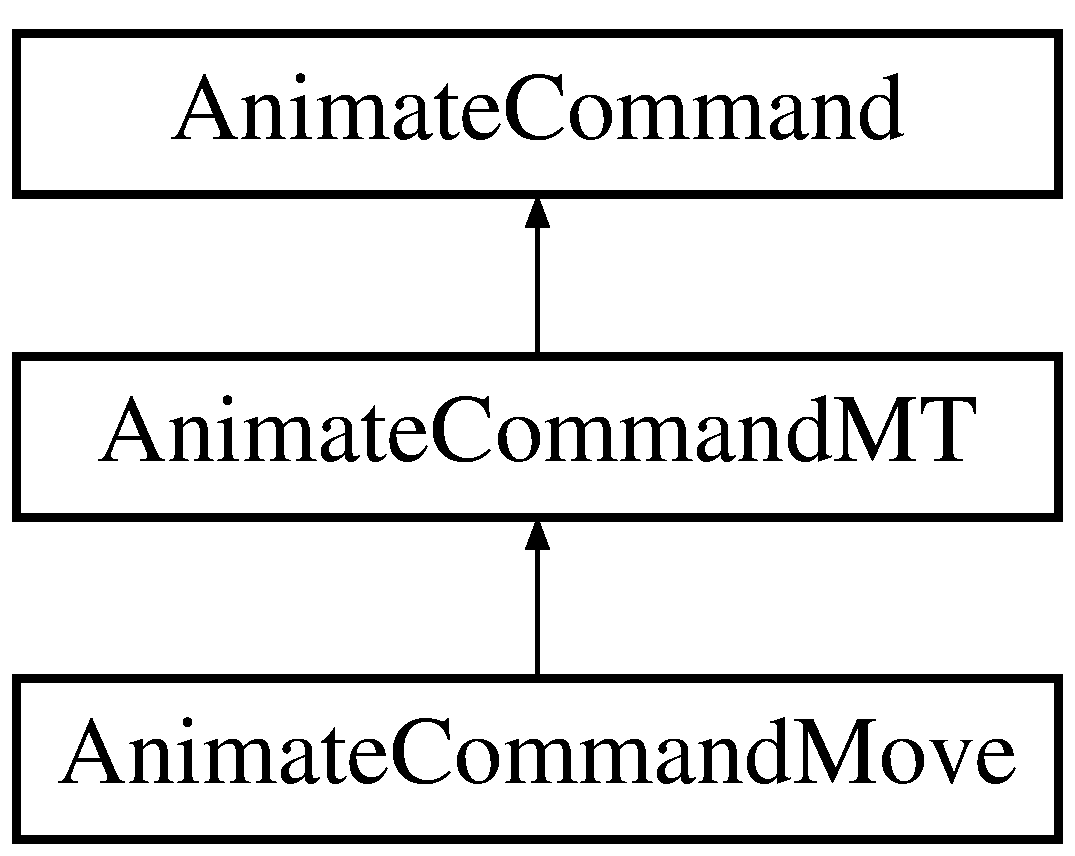
\includegraphics[height=3.000000cm]{a00005}
\end{center}
\end{figure}
\subsection*{Public Member Functions}
\begin{DoxyCompactItemize}
\item 
\hyperlink{a00005_ab1232dfcaf64d3d2aad184025fee20f0}{Animate\-Command\-M\-T} (unsigned beats, float direction)
\item 
virtual \hyperlink{a00005_acac75714a87676b065d6d2018783d540}{$\sim$\-Animate\-Command\-M\-T} ()
\item 
virtual \hyperlink{a00196_a6feaf30c8830fe6fcc0982cb7e9621ab}{Animate\-Dir} \hyperlink{a00005_a0f746d2dce20a8159f4534e555079501}{Direction} () const 
\item 
virtual float \hyperlink{a00005_a09339d867d2968b5db48faf0f9cc4891}{Real\-Direction} () const 
\end{DoxyCompactItemize}
\subsection*{Protected Attributes}
\begin{DoxyCompactItemize}
\item 
\hyperlink{a00196_a6feaf30c8830fe6fcc0982cb7e9621ab}{Animate\-Dir} \hyperlink{a00005_a206ae9756a75955c6ce573c5786bd238}{dir}
\item 
float \hyperlink{a00005_a183ee462c47adaabcdfb5391c68e3adf}{realdir}
\end{DoxyCompactItemize}


\subsection{Constructor \& Destructor Documentation}
\hypertarget{a00005_ab1232dfcaf64d3d2aad184025fee20f0}{\index{Animate\-Command\-M\-T@{Animate\-Command\-M\-T}!Animate\-Command\-M\-T@{Animate\-Command\-M\-T}}
\index{Animate\-Command\-M\-T@{Animate\-Command\-M\-T}!AnimateCommandMT@{Animate\-Command\-M\-T}}
\subsubsection[{Animate\-Command\-M\-T}]{\setlength{\rightskip}{0pt plus 5cm}Animate\-Command\-M\-T\-::\-Animate\-Command\-M\-T (
\begin{DoxyParamCaption}
\item[{unsigned}]{beats, }
\item[{float}]{direction}
\end{DoxyParamCaption}
)}}\label{a00005_ab1232dfcaf64d3d2aad184025fee20f0}
\hypertarget{a00005_acac75714a87676b065d6d2018783d540}{\index{Animate\-Command\-M\-T@{Animate\-Command\-M\-T}!$\sim$\-Animate\-Command\-M\-T@{$\sim$\-Animate\-Command\-M\-T}}
\index{$\sim$\-Animate\-Command\-M\-T@{$\sim$\-Animate\-Command\-M\-T}!AnimateCommandMT@{Animate\-Command\-M\-T}}
\subsubsection[{$\sim$\-Animate\-Command\-M\-T}]{\setlength{\rightskip}{0pt plus 5cm}virtual Animate\-Command\-M\-T\-::$\sim$\-Animate\-Command\-M\-T (
\begin{DoxyParamCaption}
{}
\end{DoxyParamCaption}
)\hspace{0.3cm}{\ttfamily [inline]}, {\ttfamily [virtual]}}}\label{a00005_acac75714a87676b065d6d2018783d540}


\subsection{Member Function Documentation}
\hypertarget{a00005_a0f746d2dce20a8159f4534e555079501}{\index{Animate\-Command\-M\-T@{Animate\-Command\-M\-T}!Direction@{Direction}}
\index{Direction@{Direction}!AnimateCommandMT@{Animate\-Command\-M\-T}}
\subsubsection[{Direction}]{\setlength{\rightskip}{0pt plus 5cm}{\bf Animate\-Dir} Animate\-Command\-M\-T\-::\-Direction (
\begin{DoxyParamCaption}
{}
\end{DoxyParamCaption}
) const\hspace{0.3cm}{\ttfamily [virtual]}}}\label{a00005_a0f746d2dce20a8159f4534e555079501}


Implements \hyperlink{a00003_ada84c0464a78c98eb9b24e64f1ea2e36}{Animate\-Command}.

\hypertarget{a00005_a09339d867d2968b5db48faf0f9cc4891}{\index{Animate\-Command\-M\-T@{Animate\-Command\-M\-T}!Real\-Direction@{Real\-Direction}}
\index{Real\-Direction@{Real\-Direction}!AnimateCommandMT@{Animate\-Command\-M\-T}}
\subsubsection[{Real\-Direction}]{\setlength{\rightskip}{0pt plus 5cm}float Animate\-Command\-M\-T\-::\-Real\-Direction (
\begin{DoxyParamCaption}
{}
\end{DoxyParamCaption}
) const\hspace{0.3cm}{\ttfamily [virtual]}}}\label{a00005_a09339d867d2968b5db48faf0f9cc4891}


Implements \hyperlink{a00003_a23b1c7a078df01cb31adaad24d29c27d}{Animate\-Command}.



\subsection{Member Data Documentation}
\hypertarget{a00005_a206ae9756a75955c6ce573c5786bd238}{\index{Animate\-Command\-M\-T@{Animate\-Command\-M\-T}!dir@{dir}}
\index{dir@{dir}!AnimateCommandMT@{Animate\-Command\-M\-T}}
\subsubsection[{dir}]{\setlength{\rightskip}{0pt plus 5cm}{\bf Animate\-Dir} Animate\-Command\-M\-T\-::dir\hspace{0.3cm}{\ttfamily [protected]}}}\label{a00005_a206ae9756a75955c6ce573c5786bd238}
\hypertarget{a00005_a183ee462c47adaabcdfb5391c68e3adf}{\index{Animate\-Command\-M\-T@{Animate\-Command\-M\-T}!realdir@{realdir}}
\index{realdir@{realdir}!AnimateCommandMT@{Animate\-Command\-M\-T}}
\subsubsection[{realdir}]{\setlength{\rightskip}{0pt plus 5cm}float Animate\-Command\-M\-T\-::realdir\hspace{0.3cm}{\ttfamily [protected]}}}\label{a00005_a183ee462c47adaabcdfb5391c68e3adf}


The documentation for this class was generated from the following files\-:\begin{DoxyCompactItemize}
\item 
src/core/\hyperlink{a00198}{animatecommand.\-h}\item 
src/core/\hyperlink{a00197}{animatecommand.\-cpp}\end{DoxyCompactItemize}

\hypertarget{a00006}{\section{Animate\-Command\-Rotate Class Reference}
\label{a00006}\index{Animate\-Command\-Rotate@{Animate\-Command\-Rotate}}
}


{\ttfamily \#include $<$animatecommand.\-h$>$}

Inheritance diagram for Animate\-Command\-Rotate\-:\begin{figure}[H]
\begin{center}
\leavevmode
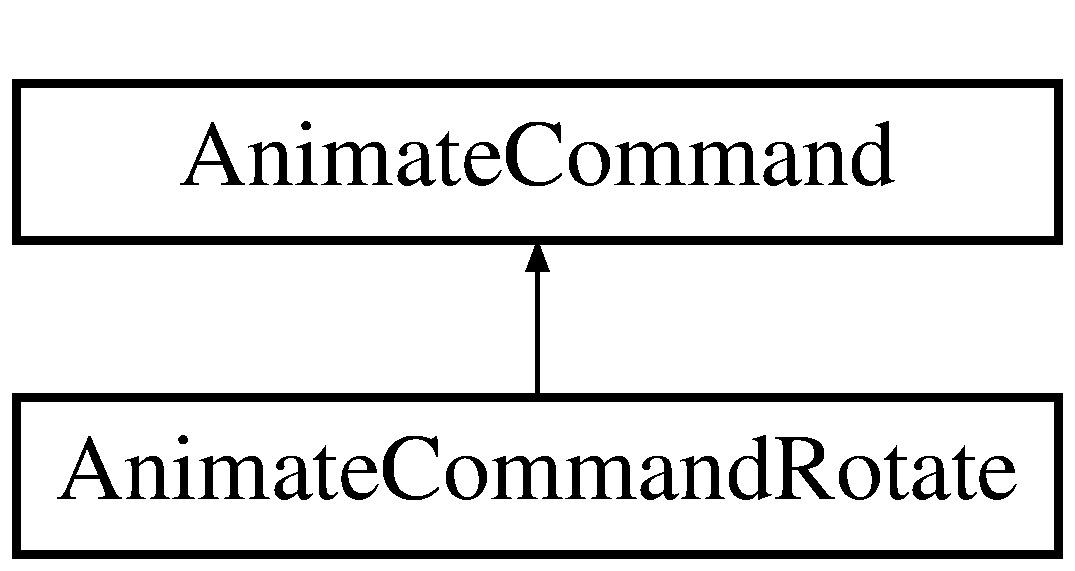
\includegraphics[height=2.000000cm]{a00006}
\end{center}
\end{figure}
\subsection*{Public Member Functions}
\begin{DoxyCompactItemize}
\item 
\hyperlink{a00006_abe77dd3438d47f7b7683bad57fc7f387}{Animate\-Command\-Rotate} (unsigned beats, \hyperlink{a00029}{C\-C\-\_\-coord} cntr, float rad, float ang1, float ang2, bool backwards=false)
\item 
virtual \hyperlink{a00006_a64bcc3164c4df08efe08c67d1498c3dd}{$\sim$\-Animate\-Command\-Rotate} ()
\item 
virtual bool \hyperlink{a00006_a5d1ee680f19374391a6fbccdcd6b6bb7}{Next\-Beat} (\hyperlink{a00196_a91212e6bb797b2b440819b6a9a86f702}{Animate\-Point} \&pt)
\item 
virtual bool \hyperlink{a00006_a179b843d1c400020f0fbb106a09c38e5}{Prev\-Beat} (\hyperlink{a00196_a91212e6bb797b2b440819b6a9a86f702}{Animate\-Point} \&pt)
\item 
virtual void \hyperlink{a00006_a0ef1ae2cc3ca46a734b231bb38347f79}{Apply\-Forward} (\hyperlink{a00196_a91212e6bb797b2b440819b6a9a86f702}{Animate\-Point} \&pt)
\item 
virtual void \hyperlink{a00006_af8f47135c6190dc9363a4d7705ad443a}{Apply\-Backward} (\hyperlink{a00196_a91212e6bb797b2b440819b6a9a86f702}{Animate\-Point} \&pt)
\item 
virtual \hyperlink{a00196_a6feaf30c8830fe6fcc0982cb7e9621ab}{Animate\-Dir} \hyperlink{a00006_ad534024d6bd630dfc0cde5e07649094a}{Direction} () const 
\item 
virtual float \hyperlink{a00006_afd366a7d56e16f296a80faab4ffe4972}{Real\-Direction} () const 
\item 
virtual void \hyperlink{a00006_a865113f57c577626241256ab35981834}{Clip\-Beats} (unsigned beats)
\item 
virtual \hyperlink{a00031}{C\-C\-\_\-\-Draw\-Command} \hyperlink{a00006_a999e00a33481237a53af76481913d83f}{Gen\-C\-C\-\_\-\-Draw\-Command} (const \hyperlink{a00196_a91212e6bb797b2b440819b6a9a86f702}{Animate\-Point} \&pt, const \hyperlink{a00029}{C\-C\-\_\-coord} \&offset) const 
\end{DoxyCompactItemize}
\subsection*{Private Attributes}
\begin{DoxyCompactItemize}
\item 
\hyperlink{a00029}{C\-C\-\_\-coord} \hyperlink{a00006_a8dfd55b23f76e9f9987f8ea9e4e3239a}{m\-Origin}
\item 
float \hyperlink{a00006_a1a720ab7b39b95a6a8116308f50b02a8}{m\-R}
\item 
float \hyperlink{a00006_a50c782c031d209ac040c71b0792be40e}{m\-Ang\-Start}
\item 
float \hyperlink{a00006_a03d54f905dbfd4927a10e4f9e23fcfb9}{m\-Ang\-End}
\item 
float \hyperlink{a00006_aa513da05df7bf1998098c4fc9234a1e5}{m\-Face}
\end{DoxyCompactItemize}
\subsection*{Additional Inherited Members}


\subsection{Constructor \& Destructor Documentation}
\hypertarget{a00006_abe77dd3438d47f7b7683bad57fc7f387}{\index{Animate\-Command\-Rotate@{Animate\-Command\-Rotate}!Animate\-Command\-Rotate@{Animate\-Command\-Rotate}}
\index{Animate\-Command\-Rotate@{Animate\-Command\-Rotate}!AnimateCommandRotate@{Animate\-Command\-Rotate}}
\subsubsection[{Animate\-Command\-Rotate}]{\setlength{\rightskip}{0pt plus 5cm}Animate\-Command\-Rotate\-::\-Animate\-Command\-Rotate (
\begin{DoxyParamCaption}
\item[{unsigned}]{beats, }
\item[{{\bf C\-C\-\_\-coord}}]{cntr, }
\item[{float}]{rad, }
\item[{float}]{ang1, }
\item[{float}]{ang2, }
\item[{bool}]{backwards = {\ttfamily false}}
\end{DoxyParamCaption}
)}}\label{a00006_abe77dd3438d47f7b7683bad57fc7f387}
\hypertarget{a00006_a64bcc3164c4df08efe08c67d1498c3dd}{\index{Animate\-Command\-Rotate@{Animate\-Command\-Rotate}!$\sim$\-Animate\-Command\-Rotate@{$\sim$\-Animate\-Command\-Rotate}}
\index{$\sim$\-Animate\-Command\-Rotate@{$\sim$\-Animate\-Command\-Rotate}!AnimateCommandRotate@{Animate\-Command\-Rotate}}
\subsubsection[{$\sim$\-Animate\-Command\-Rotate}]{\setlength{\rightskip}{0pt plus 5cm}virtual Animate\-Command\-Rotate\-::$\sim$\-Animate\-Command\-Rotate (
\begin{DoxyParamCaption}
{}
\end{DoxyParamCaption}
)\hspace{0.3cm}{\ttfamily [inline]}, {\ttfamily [virtual]}}}\label{a00006_a64bcc3164c4df08efe08c67d1498c3dd}


\subsection{Member Function Documentation}
\hypertarget{a00006_af8f47135c6190dc9363a4d7705ad443a}{\index{Animate\-Command\-Rotate@{Animate\-Command\-Rotate}!Apply\-Backward@{Apply\-Backward}}
\index{Apply\-Backward@{Apply\-Backward}!AnimateCommandRotate@{Animate\-Command\-Rotate}}
\subsubsection[{Apply\-Backward}]{\setlength{\rightskip}{0pt plus 5cm}void Animate\-Command\-Rotate\-::\-Apply\-Backward (
\begin{DoxyParamCaption}
\item[{{\bf Animate\-Point} \&}]{pt}
\end{DoxyParamCaption}
)\hspace{0.3cm}{\ttfamily [virtual]}}}\label{a00006_af8f47135c6190dc9363a4d7705ad443a}


Reimplemented from \hyperlink{a00003_a969de0c473c2ca7d2f3b9ea8748fffb7}{Animate\-Command}.

\hypertarget{a00006_a0ef1ae2cc3ca46a734b231bb38347f79}{\index{Animate\-Command\-Rotate@{Animate\-Command\-Rotate}!Apply\-Forward@{Apply\-Forward}}
\index{Apply\-Forward@{Apply\-Forward}!AnimateCommandRotate@{Animate\-Command\-Rotate}}
\subsubsection[{Apply\-Forward}]{\setlength{\rightskip}{0pt plus 5cm}void Animate\-Command\-Rotate\-::\-Apply\-Forward (
\begin{DoxyParamCaption}
\item[{{\bf Animate\-Point} \&}]{pt}
\end{DoxyParamCaption}
)\hspace{0.3cm}{\ttfamily [virtual]}}}\label{a00006_a0ef1ae2cc3ca46a734b231bb38347f79}


Reimplemented from \hyperlink{a00003_af8a485b986aacf649f41c81e4d6eeed9}{Animate\-Command}.

\hypertarget{a00006_a865113f57c577626241256ab35981834}{\index{Animate\-Command\-Rotate@{Animate\-Command\-Rotate}!Clip\-Beats@{Clip\-Beats}}
\index{Clip\-Beats@{Clip\-Beats}!AnimateCommandRotate@{Animate\-Command\-Rotate}}
\subsubsection[{Clip\-Beats}]{\setlength{\rightskip}{0pt plus 5cm}void Animate\-Command\-Rotate\-::\-Clip\-Beats (
\begin{DoxyParamCaption}
\item[{unsigned}]{beats}
\end{DoxyParamCaption}
)\hspace{0.3cm}{\ttfamily [virtual]}}}\label{a00006_a865113f57c577626241256ab35981834}


Reimplemented from \hyperlink{a00003_ace20ca13c14bf94e13404df0ef825da8}{Animate\-Command}.

\hypertarget{a00006_ad534024d6bd630dfc0cde5e07649094a}{\index{Animate\-Command\-Rotate@{Animate\-Command\-Rotate}!Direction@{Direction}}
\index{Direction@{Direction}!AnimateCommandRotate@{Animate\-Command\-Rotate}}
\subsubsection[{Direction}]{\setlength{\rightskip}{0pt plus 5cm}{\bf Animate\-Dir} Animate\-Command\-Rotate\-::\-Direction (
\begin{DoxyParamCaption}
{}
\end{DoxyParamCaption}
) const\hspace{0.3cm}{\ttfamily [virtual]}}}\label{a00006_ad534024d6bd630dfc0cde5e07649094a}


Implements \hyperlink{a00003_ada84c0464a78c98eb9b24e64f1ea2e36}{Animate\-Command}.

\hypertarget{a00006_a999e00a33481237a53af76481913d83f}{\index{Animate\-Command\-Rotate@{Animate\-Command\-Rotate}!Gen\-C\-C\-\_\-\-Draw\-Command@{Gen\-C\-C\-\_\-\-Draw\-Command}}
\index{Gen\-C\-C\-\_\-\-Draw\-Command@{Gen\-C\-C\-\_\-\-Draw\-Command}!AnimateCommandRotate@{Animate\-Command\-Rotate}}
\subsubsection[{Gen\-C\-C\-\_\-\-Draw\-Command}]{\setlength{\rightskip}{0pt plus 5cm}{\bf C\-C\-\_\-\-Draw\-Command} Animate\-Command\-Rotate\-::\-Gen\-C\-C\-\_\-\-Draw\-Command (
\begin{DoxyParamCaption}
\item[{const {\bf Animate\-Point} \&}]{pt, }
\item[{const {\bf C\-C\-\_\-coord} \&}]{offset}
\end{DoxyParamCaption}
) const\hspace{0.3cm}{\ttfamily [virtual]}}}\label{a00006_a999e00a33481237a53af76481913d83f}


Reimplemented from \hyperlink{a00003_a34d8e8a89c11f7ef6d1e2346db77d462}{Animate\-Command}.

\hypertarget{a00006_a5d1ee680f19374391a6fbccdcd6b6bb7}{\index{Animate\-Command\-Rotate@{Animate\-Command\-Rotate}!Next\-Beat@{Next\-Beat}}
\index{Next\-Beat@{Next\-Beat}!AnimateCommandRotate@{Animate\-Command\-Rotate}}
\subsubsection[{Next\-Beat}]{\setlength{\rightskip}{0pt plus 5cm}bool Animate\-Command\-Rotate\-::\-Next\-Beat (
\begin{DoxyParamCaption}
\item[{{\bf Animate\-Point} \&}]{pt}
\end{DoxyParamCaption}
)\hspace{0.3cm}{\ttfamily [virtual]}}}\label{a00006_a5d1ee680f19374391a6fbccdcd6b6bb7}


Reimplemented from \hyperlink{a00003_a80bcd30c221c961d87049dee4d9eff5e}{Animate\-Command}.

\hypertarget{a00006_a179b843d1c400020f0fbb106a09c38e5}{\index{Animate\-Command\-Rotate@{Animate\-Command\-Rotate}!Prev\-Beat@{Prev\-Beat}}
\index{Prev\-Beat@{Prev\-Beat}!AnimateCommandRotate@{Animate\-Command\-Rotate}}
\subsubsection[{Prev\-Beat}]{\setlength{\rightskip}{0pt plus 5cm}bool Animate\-Command\-Rotate\-::\-Prev\-Beat (
\begin{DoxyParamCaption}
\item[{{\bf Animate\-Point} \&}]{pt}
\end{DoxyParamCaption}
)\hspace{0.3cm}{\ttfamily [virtual]}}}\label{a00006_a179b843d1c400020f0fbb106a09c38e5}


Reimplemented from \hyperlink{a00003_aafde773d0e8074306eed850c91c7f207}{Animate\-Command}.

\hypertarget{a00006_afd366a7d56e16f296a80faab4ffe4972}{\index{Animate\-Command\-Rotate@{Animate\-Command\-Rotate}!Real\-Direction@{Real\-Direction}}
\index{Real\-Direction@{Real\-Direction}!AnimateCommandRotate@{Animate\-Command\-Rotate}}
\subsubsection[{Real\-Direction}]{\setlength{\rightskip}{0pt plus 5cm}float Animate\-Command\-Rotate\-::\-Real\-Direction (
\begin{DoxyParamCaption}
{}
\end{DoxyParamCaption}
) const\hspace{0.3cm}{\ttfamily [virtual]}}}\label{a00006_afd366a7d56e16f296a80faab4ffe4972}


Implements \hyperlink{a00003_a23b1c7a078df01cb31adaad24d29c27d}{Animate\-Command}.



\subsection{Member Data Documentation}
\hypertarget{a00006_a03d54f905dbfd4927a10e4f9e23fcfb9}{\index{Animate\-Command\-Rotate@{Animate\-Command\-Rotate}!m\-Ang\-End@{m\-Ang\-End}}
\index{m\-Ang\-End@{m\-Ang\-End}!AnimateCommandRotate@{Animate\-Command\-Rotate}}
\subsubsection[{m\-Ang\-End}]{\setlength{\rightskip}{0pt plus 5cm}float Animate\-Command\-Rotate\-::m\-Ang\-End\hspace{0.3cm}{\ttfamily [private]}}}\label{a00006_a03d54f905dbfd4927a10e4f9e23fcfb9}
\hypertarget{a00006_a50c782c031d209ac040c71b0792be40e}{\index{Animate\-Command\-Rotate@{Animate\-Command\-Rotate}!m\-Ang\-Start@{m\-Ang\-Start}}
\index{m\-Ang\-Start@{m\-Ang\-Start}!AnimateCommandRotate@{Animate\-Command\-Rotate}}
\subsubsection[{m\-Ang\-Start}]{\setlength{\rightskip}{0pt plus 5cm}float Animate\-Command\-Rotate\-::m\-Ang\-Start\hspace{0.3cm}{\ttfamily [private]}}}\label{a00006_a50c782c031d209ac040c71b0792be40e}
\hypertarget{a00006_aa513da05df7bf1998098c4fc9234a1e5}{\index{Animate\-Command\-Rotate@{Animate\-Command\-Rotate}!m\-Face@{m\-Face}}
\index{m\-Face@{m\-Face}!AnimateCommandRotate@{Animate\-Command\-Rotate}}
\subsubsection[{m\-Face}]{\setlength{\rightskip}{0pt plus 5cm}float Animate\-Command\-Rotate\-::m\-Face\hspace{0.3cm}{\ttfamily [private]}}}\label{a00006_aa513da05df7bf1998098c4fc9234a1e5}
\hypertarget{a00006_a8dfd55b23f76e9f9987f8ea9e4e3239a}{\index{Animate\-Command\-Rotate@{Animate\-Command\-Rotate}!m\-Origin@{m\-Origin}}
\index{m\-Origin@{m\-Origin}!AnimateCommandRotate@{Animate\-Command\-Rotate}}
\subsubsection[{m\-Origin}]{\setlength{\rightskip}{0pt plus 5cm}{\bf C\-C\-\_\-coord} Animate\-Command\-Rotate\-::m\-Origin\hspace{0.3cm}{\ttfamily [private]}}}\label{a00006_a8dfd55b23f76e9f9987f8ea9e4e3239a}
\hypertarget{a00006_a1a720ab7b39b95a6a8116308f50b02a8}{\index{Animate\-Command\-Rotate@{Animate\-Command\-Rotate}!m\-R@{m\-R}}
\index{m\-R@{m\-R}!AnimateCommandRotate@{Animate\-Command\-Rotate}}
\subsubsection[{m\-R}]{\setlength{\rightskip}{0pt plus 5cm}float Animate\-Command\-Rotate\-::m\-R\hspace{0.3cm}{\ttfamily [private]}}}\label{a00006_a1a720ab7b39b95a6a8116308f50b02a8}


The documentation for this class was generated from the following files\-:\begin{DoxyCompactItemize}
\item 
src/core/\hyperlink{a00198}{animatecommand.\-h}\item 
src/core/\hyperlink{a00197}{animatecommand.\-cpp}\end{DoxyCompactItemize}

\hypertarget{a00007}{\section{Animate\-Compile Class Reference}
\label{a00007}\index{Animate\-Compile@{Animate\-Compile}}
}


{\ttfamily \#include $<$animatecompile.\-h$>$}

\subsection*{Public Member Functions}
\begin{DoxyCompactItemize}
\item 
\hyperlink{a00007_a7b3f8a2ace64c939aa76225984e25c04}{Animate\-Compile} (const \hyperlink{a00046}{C\-C\-\_\-show} \&show, \hyperlink{a00014}{Animation\-Variables} \&variables\-States)
\item 
\hyperlink{a00007_a8a621790c421b2b1ff10a2a8b3f49fab}{$\sim$\-Animate\-Compile} ()
\item 
std\-::vector$<$ boost\-::shared\-\_\-ptr\\*
$<$ \hyperlink{a00003}{Animate\-Command} $>$ $>$ \hyperlink{a00007_a34cceb61b18c2ae436efe5f95becb28a}{Compile} (\hyperlink{a00046_aaaf1345012d2f833d1c8f28f9b8593ff}{C\-C\-\_\-show\-::const\-\_\-\-C\-C\-\_\-sheet\-\_\-iterator\-\_\-t} c\-\_\-sheet, unsigned pt\-\_\-num, \hyperlink{a00216_a68cd84e0300be6f9ff4474682762c9ee}{S\-Y\-M\-B\-O\-L\-\_\-\-T\-Y\-P\-E} cont\-\_\-symbol, \hyperlink{a00067}{Cont\-Procedure} $\ast$proc)
\item 
bool \hyperlink{a00007_a2eab2ee0c43db362a33e54abb941c057}{Append} (boost\-::shared\-\_\-ptr$<$ \hyperlink{a00003}{Animate\-Command} $>$ cmd, const \hyperlink{a00085}{Cont\-Token} $\ast$token)
\item 
bool \hyperlink{a00007_a712b8954d7ef78f56cda0601984986d3}{Okay} ()
\item 
void \hyperlink{a00007_aad974c45b5dac1d240ede102fc664e02}{Register\-Error} (\hyperlink{a00196_a85ee9a09c66824778f4d1e44411f8703}{Animate\-Error} err, const \hyperlink{a00085}{Cont\-Token} $\ast$token)
\item 
float \hyperlink{a00007_a8a1eabe9a7e81917cd67c7c96266dc7e}{Get\-Var\-Value} (int varnum, const \hyperlink{a00085}{Cont\-Token} $\ast$token)
\item 
void \hyperlink{a00007_aa12ee95a9e8e604454ac2ce772cb9c44}{Set\-Var\-Value} (int varnum, float value)
\item 
std\-::vector$<$ \hyperlink{a00098}{Error\-Marker} $>$ \hyperlink{a00007_a1cce4acfa8fd114785068f74def98992}{Get\-Error\-Markers} () const 
\item 
\hyperlink{a00196_a91212e6bb797b2b440819b6a9a86f702}{Animate\-Point} \hyperlink{a00007_ae670d64339321051cbb382525530eff0}{Get\-Point\-Position} () const 
\item 
unsigned \hyperlink{a00007_a6406e70747c4bdc0fb8d30b5e71bf3b2}{Get\-Current\-Point} () const 
\item 
unsigned \hyperlink{a00007_a3d824c8de9d6e906a6d14d5011ded73f}{Get\-Beats\-Remaining} () const 
\item 
\hyperlink{a00196_a91212e6bb797b2b440819b6a9a86f702}{Animate\-Point} \hyperlink{a00007_ae4ba7526a293c2cdbada00e592bd21a6}{Get\-Starting\-Position} () const 
\item 
\hyperlink{a00196_a91212e6bb797b2b440819b6a9a86f702}{Animate\-Point} \hyperlink{a00007_afe8f5e9a0d727dc134497a1783ca7656}{Get\-Ending\-Position} (const \hyperlink{a00085}{Cont\-Token} $\ast$token)
\item 
\hyperlink{a00196_a91212e6bb797b2b440819b6a9a86f702}{Animate\-Point} \hyperlink{a00007_ab55c26d9886d951d63f9415e653e865c}{Get\-Reference\-Point\-Position} (unsigned refnum) const 
\end{DoxyCompactItemize}
\subsection*{Private Member Functions}
\begin{DoxyCompactItemize}
\item 
void \hyperlink{a00007_a1fafdaa29093c8abfc725a9dad511966}{Set\-Status} (bool s)
\end{DoxyCompactItemize}
\subsection*{Private Attributes}
\begin{DoxyCompactItemize}
\item 
\hyperlink{a00196_a91212e6bb797b2b440819b6a9a86f702}{Animate\-Point} \hyperlink{a00007_a452baa7903c665a4861cb1f1eaa9d2df}{pt}
\item 
const \hyperlink{a00046}{C\-C\-\_\-show} \& \hyperlink{a00007_abf4e08c9790e8d8e011de3c2b8120ecd}{m\-Show}
\item 
\hyperlink{a00046_aaaf1345012d2f833d1c8f28f9b8593ff}{C\-C\-\_\-show\-::const\-\_\-\-C\-C\-\_\-sheet\-\_\-iterator\-\_\-t} \hyperlink{a00007_a506679d533380355bf4de8b9f4d8aaa1}{curr\-\_\-sheet}
\item 
unsigned \hyperlink{a00007_a88dedadc61cd7a2dcc08140809e81e0b}{curr\-\_\-pt}
\item 
unsigned \hyperlink{a00007_af3feb682c6ad3aab1c7483d6b3dcd5f0}{beats\-\_\-rem}
\item 
\hyperlink{a00216_a68cd84e0300be6f9ff4474682762c9ee}{S\-Y\-M\-B\-O\-L\-\_\-\-T\-Y\-P\-E} \hyperlink{a00007_aa854b256cdb3fcc21d3a7b110f34bc20}{contsymbol}
\item 
std\-::vector$<$ boost\-::shared\-\_\-ptr\\*
$<$ \hyperlink{a00003}{Animate\-Command} $>$ $>$ \hyperlink{a00007_a5d5b0775236c5ad6382eb58f1e0fc0a9}{cmds}
\item 
std\-::vector$<$ \hyperlink{a00098}{Error\-Marker} $>$ \hyperlink{a00007_a727a78d36a18425535c2d262ee7634b2}{error\-\_\-markers}
\item 
\hyperlink{a00014}{Animation\-Variables} \& \hyperlink{a00007_a5bb5e56e9ad574dc86439a37eb4511c7}{vars}
\item 
bool \hyperlink{a00007_a937c6b3e6577b594848cc98b62915ede}{okay}
\end{DoxyCompactItemize}


\subsection{Constructor \& Destructor Documentation}
\hypertarget{a00007_a7b3f8a2ace64c939aa76225984e25c04}{\index{Animate\-Compile@{Animate\-Compile}!Animate\-Compile@{Animate\-Compile}}
\index{Animate\-Compile@{Animate\-Compile}!AnimateCompile@{Animate\-Compile}}
\subsubsection[{Animate\-Compile}]{\setlength{\rightskip}{0pt plus 5cm}Animate\-Compile\-::\-Animate\-Compile (
\begin{DoxyParamCaption}
\item[{const {\bf C\-C\-\_\-show} \&}]{show, }
\item[{{\bf Animation\-Variables} \&}]{variables\-States}
\end{DoxyParamCaption}
)}}\label{a00007_a7b3f8a2ace64c939aa76225984e25c04}
\hypertarget{a00007_a8a621790c421b2b1ff10a2a8b3f49fab}{\index{Animate\-Compile@{Animate\-Compile}!$\sim$\-Animate\-Compile@{$\sim$\-Animate\-Compile}}
\index{$\sim$\-Animate\-Compile@{$\sim$\-Animate\-Compile}!AnimateCompile@{Animate\-Compile}}
\subsubsection[{$\sim$\-Animate\-Compile}]{\setlength{\rightskip}{0pt plus 5cm}Animate\-Compile\-::$\sim$\-Animate\-Compile (
\begin{DoxyParamCaption}
{}
\end{DoxyParamCaption}
)}}\label{a00007_a8a621790c421b2b1ff10a2a8b3f49fab}


\subsection{Member Function Documentation}
\hypertarget{a00007_a2eab2ee0c43db362a33e54abb941c057}{\index{Animate\-Compile@{Animate\-Compile}!Append@{Append}}
\index{Append@{Append}!AnimateCompile@{Animate\-Compile}}
\subsubsection[{Append}]{\setlength{\rightskip}{0pt plus 5cm}bool Animate\-Compile\-::\-Append (
\begin{DoxyParamCaption}
\item[{boost\-::shared\-\_\-ptr$<$ {\bf Animate\-Command} $>$}]{cmd, }
\item[{const {\bf Cont\-Token} $\ast$}]{token}
\end{DoxyParamCaption}
)}}\label{a00007_a2eab2ee0c43db362a33e54abb941c057}
\hypertarget{a00007_a34cceb61b18c2ae436efe5f95becb28a}{\index{Animate\-Compile@{Animate\-Compile}!Compile@{Compile}}
\index{Compile@{Compile}!AnimateCompile@{Animate\-Compile}}
\subsubsection[{Compile}]{\setlength{\rightskip}{0pt plus 5cm}std\-::vector$<$ boost\-::shared\-\_\-ptr$<$ {\bf Animate\-Command} $>$ $>$ Animate\-Compile\-::\-Compile (
\begin{DoxyParamCaption}
\item[{{\bf C\-C\-\_\-show\-::const\-\_\-\-C\-C\-\_\-sheet\-\_\-iterator\-\_\-t}}]{c\-\_\-sheet, }
\item[{unsigned}]{pt\-\_\-num, }
\item[{{\bf S\-Y\-M\-B\-O\-L\-\_\-\-T\-Y\-P\-E}}]{cont\-\_\-symbol, }
\item[{{\bf Cont\-Procedure} $\ast$}]{proc}
\end{DoxyParamCaption}
)}}\label{a00007_a34cceb61b18c2ae436efe5f95becb28a}
\hypertarget{a00007_a3d824c8de9d6e906a6d14d5011ded73f}{\index{Animate\-Compile@{Animate\-Compile}!Get\-Beats\-Remaining@{Get\-Beats\-Remaining}}
\index{Get\-Beats\-Remaining@{Get\-Beats\-Remaining}!AnimateCompile@{Animate\-Compile}}
\subsubsection[{Get\-Beats\-Remaining}]{\setlength{\rightskip}{0pt plus 5cm}unsigned Animate\-Compile\-::\-Get\-Beats\-Remaining (
\begin{DoxyParamCaption}
{}
\end{DoxyParamCaption}
) const\hspace{0.3cm}{\ttfamily [inline]}}}\label{a00007_a3d824c8de9d6e906a6d14d5011ded73f}
\hypertarget{a00007_a6406e70747c4bdc0fb8d30b5e71bf3b2}{\index{Animate\-Compile@{Animate\-Compile}!Get\-Current\-Point@{Get\-Current\-Point}}
\index{Get\-Current\-Point@{Get\-Current\-Point}!AnimateCompile@{Animate\-Compile}}
\subsubsection[{Get\-Current\-Point}]{\setlength{\rightskip}{0pt plus 5cm}unsigned Animate\-Compile\-::\-Get\-Current\-Point (
\begin{DoxyParamCaption}
{}
\end{DoxyParamCaption}
) const\hspace{0.3cm}{\ttfamily [inline]}}}\label{a00007_a6406e70747c4bdc0fb8d30b5e71bf3b2}
\hypertarget{a00007_afe8f5e9a0d727dc134497a1783ca7656}{\index{Animate\-Compile@{Animate\-Compile}!Get\-Ending\-Position@{Get\-Ending\-Position}}
\index{Get\-Ending\-Position@{Get\-Ending\-Position}!AnimateCompile@{Animate\-Compile}}
\subsubsection[{Get\-Ending\-Position}]{\setlength{\rightskip}{0pt plus 5cm}{\bf Animate\-Point} Animate\-Compile\-::\-Get\-Ending\-Position (
\begin{DoxyParamCaption}
\item[{const {\bf Cont\-Token} $\ast$}]{token}
\end{DoxyParamCaption}
)}}\label{a00007_afe8f5e9a0d727dc134497a1783ca7656}
\hypertarget{a00007_a1cce4acfa8fd114785068f74def98992}{\index{Animate\-Compile@{Animate\-Compile}!Get\-Error\-Markers@{Get\-Error\-Markers}}
\index{Get\-Error\-Markers@{Get\-Error\-Markers}!AnimateCompile@{Animate\-Compile}}
\subsubsection[{Get\-Error\-Markers}]{\setlength{\rightskip}{0pt plus 5cm}std\-::vector$<${\bf Error\-Marker}$>$ Animate\-Compile\-::\-Get\-Error\-Markers (
\begin{DoxyParamCaption}
{}
\end{DoxyParamCaption}
) const\hspace{0.3cm}{\ttfamily [inline]}}}\label{a00007_a1cce4acfa8fd114785068f74def98992}
\hypertarget{a00007_ae670d64339321051cbb382525530eff0}{\index{Animate\-Compile@{Animate\-Compile}!Get\-Point\-Position@{Get\-Point\-Position}}
\index{Get\-Point\-Position@{Get\-Point\-Position}!AnimateCompile@{Animate\-Compile}}
\subsubsection[{Get\-Point\-Position}]{\setlength{\rightskip}{0pt plus 5cm}{\bf Animate\-Point} Animate\-Compile\-::\-Get\-Point\-Position (
\begin{DoxyParamCaption}
{}
\end{DoxyParamCaption}
) const\hspace{0.3cm}{\ttfamily [inline]}}}\label{a00007_ae670d64339321051cbb382525530eff0}
\hypertarget{a00007_ab55c26d9886d951d63f9415e653e865c}{\index{Animate\-Compile@{Animate\-Compile}!Get\-Reference\-Point\-Position@{Get\-Reference\-Point\-Position}}
\index{Get\-Reference\-Point\-Position@{Get\-Reference\-Point\-Position}!AnimateCompile@{Animate\-Compile}}
\subsubsection[{Get\-Reference\-Point\-Position}]{\setlength{\rightskip}{0pt plus 5cm}{\bf Animate\-Point} Animate\-Compile\-::\-Get\-Reference\-Point\-Position (
\begin{DoxyParamCaption}
\item[{unsigned}]{refnum}
\end{DoxyParamCaption}
) const}}\label{a00007_ab55c26d9886d951d63f9415e653e865c}
\hypertarget{a00007_ae4ba7526a293c2cdbada00e592bd21a6}{\index{Animate\-Compile@{Animate\-Compile}!Get\-Starting\-Position@{Get\-Starting\-Position}}
\index{Get\-Starting\-Position@{Get\-Starting\-Position}!AnimateCompile@{Animate\-Compile}}
\subsubsection[{Get\-Starting\-Position}]{\setlength{\rightskip}{0pt plus 5cm}{\bf Animate\-Point} Animate\-Compile\-::\-Get\-Starting\-Position (
\begin{DoxyParamCaption}
{}
\end{DoxyParamCaption}
) const}}\label{a00007_ae4ba7526a293c2cdbada00e592bd21a6}
\hypertarget{a00007_a8a1eabe9a7e81917cd67c7c96266dc7e}{\index{Animate\-Compile@{Animate\-Compile}!Get\-Var\-Value@{Get\-Var\-Value}}
\index{Get\-Var\-Value@{Get\-Var\-Value}!AnimateCompile@{Animate\-Compile}}
\subsubsection[{Get\-Var\-Value}]{\setlength{\rightskip}{0pt plus 5cm}float Animate\-Compile\-::\-Get\-Var\-Value (
\begin{DoxyParamCaption}
\item[{int}]{varnum, }
\item[{const {\bf Cont\-Token} $\ast$}]{token}
\end{DoxyParamCaption}
)}}\label{a00007_a8a1eabe9a7e81917cd67c7c96266dc7e}
\hypertarget{a00007_a712b8954d7ef78f56cda0601984986d3}{\index{Animate\-Compile@{Animate\-Compile}!Okay@{Okay}}
\index{Okay@{Okay}!AnimateCompile@{Animate\-Compile}}
\subsubsection[{Okay}]{\setlength{\rightskip}{0pt plus 5cm}bool Animate\-Compile\-::\-Okay (
\begin{DoxyParamCaption}
{}
\end{DoxyParamCaption}
)\hspace{0.3cm}{\ttfamily [inline]}}}\label{a00007_a712b8954d7ef78f56cda0601984986d3}
\hypertarget{a00007_aad974c45b5dac1d240ede102fc664e02}{\index{Animate\-Compile@{Animate\-Compile}!Register\-Error@{Register\-Error}}
\index{Register\-Error@{Register\-Error}!AnimateCompile@{Animate\-Compile}}
\subsubsection[{Register\-Error}]{\setlength{\rightskip}{0pt plus 5cm}void Animate\-Compile\-::\-Register\-Error (
\begin{DoxyParamCaption}
\item[{{\bf Animate\-Error}}]{err, }
\item[{const {\bf Cont\-Token} $\ast$}]{token}
\end{DoxyParamCaption}
)}}\label{a00007_aad974c45b5dac1d240ede102fc664e02}
\hypertarget{a00007_a1fafdaa29093c8abfc725a9dad511966}{\index{Animate\-Compile@{Animate\-Compile}!Set\-Status@{Set\-Status}}
\index{Set\-Status@{Set\-Status}!AnimateCompile@{Animate\-Compile}}
\subsubsection[{Set\-Status}]{\setlength{\rightskip}{0pt plus 5cm}void Animate\-Compile\-::\-Set\-Status (
\begin{DoxyParamCaption}
\item[{bool}]{s}
\end{DoxyParamCaption}
)\hspace{0.3cm}{\ttfamily [inline]}, {\ttfamily [private]}}}\label{a00007_a1fafdaa29093c8abfc725a9dad511966}
\hypertarget{a00007_aa12ee95a9e8e604454ac2ce772cb9c44}{\index{Animate\-Compile@{Animate\-Compile}!Set\-Var\-Value@{Set\-Var\-Value}}
\index{Set\-Var\-Value@{Set\-Var\-Value}!AnimateCompile@{Animate\-Compile}}
\subsubsection[{Set\-Var\-Value}]{\setlength{\rightskip}{0pt plus 5cm}void Animate\-Compile\-::\-Set\-Var\-Value (
\begin{DoxyParamCaption}
\item[{int}]{varnum, }
\item[{float}]{value}
\end{DoxyParamCaption}
)}}\label{a00007_aa12ee95a9e8e604454ac2ce772cb9c44}


\subsection{Member Data Documentation}
\hypertarget{a00007_af3feb682c6ad3aab1c7483d6b3dcd5f0}{\index{Animate\-Compile@{Animate\-Compile}!beats\-\_\-rem@{beats\-\_\-rem}}
\index{beats\-\_\-rem@{beats\-\_\-rem}!AnimateCompile@{Animate\-Compile}}
\subsubsection[{beats\-\_\-rem}]{\setlength{\rightskip}{0pt plus 5cm}unsigned Animate\-Compile\-::beats\-\_\-rem\hspace{0.3cm}{\ttfamily [private]}}}\label{a00007_af3feb682c6ad3aab1c7483d6b3dcd5f0}
\hypertarget{a00007_a5d5b0775236c5ad6382eb58f1e0fc0a9}{\index{Animate\-Compile@{Animate\-Compile}!cmds@{cmds}}
\index{cmds@{cmds}!AnimateCompile@{Animate\-Compile}}
\subsubsection[{cmds}]{\setlength{\rightskip}{0pt plus 5cm}std\-::vector$<$boost\-::shared\-\_\-ptr$<${\bf Animate\-Command}$>$ $>$ Animate\-Compile\-::cmds\hspace{0.3cm}{\ttfamily [private]}}}\label{a00007_a5d5b0775236c5ad6382eb58f1e0fc0a9}
\hypertarget{a00007_aa854b256cdb3fcc21d3a7b110f34bc20}{\index{Animate\-Compile@{Animate\-Compile}!contsymbol@{contsymbol}}
\index{contsymbol@{contsymbol}!AnimateCompile@{Animate\-Compile}}
\subsubsection[{contsymbol}]{\setlength{\rightskip}{0pt plus 5cm}{\bf S\-Y\-M\-B\-O\-L\-\_\-\-T\-Y\-P\-E} Animate\-Compile\-::contsymbol\hspace{0.3cm}{\ttfamily [private]}}}\label{a00007_aa854b256cdb3fcc21d3a7b110f34bc20}
\hypertarget{a00007_a88dedadc61cd7a2dcc08140809e81e0b}{\index{Animate\-Compile@{Animate\-Compile}!curr\-\_\-pt@{curr\-\_\-pt}}
\index{curr\-\_\-pt@{curr\-\_\-pt}!AnimateCompile@{Animate\-Compile}}
\subsubsection[{curr\-\_\-pt}]{\setlength{\rightskip}{0pt plus 5cm}unsigned Animate\-Compile\-::curr\-\_\-pt\hspace{0.3cm}{\ttfamily [private]}}}\label{a00007_a88dedadc61cd7a2dcc08140809e81e0b}
\hypertarget{a00007_a506679d533380355bf4de8b9f4d8aaa1}{\index{Animate\-Compile@{Animate\-Compile}!curr\-\_\-sheet@{curr\-\_\-sheet}}
\index{curr\-\_\-sheet@{curr\-\_\-sheet}!AnimateCompile@{Animate\-Compile}}
\subsubsection[{curr\-\_\-sheet}]{\setlength{\rightskip}{0pt plus 5cm}{\bf C\-C\-\_\-show\-::const\-\_\-\-C\-C\-\_\-sheet\-\_\-iterator\-\_\-t} Animate\-Compile\-::curr\-\_\-sheet\hspace{0.3cm}{\ttfamily [private]}}}\label{a00007_a506679d533380355bf4de8b9f4d8aaa1}
\hypertarget{a00007_a727a78d36a18425535c2d262ee7634b2}{\index{Animate\-Compile@{Animate\-Compile}!error\-\_\-markers@{error\-\_\-markers}}
\index{error\-\_\-markers@{error\-\_\-markers}!AnimateCompile@{Animate\-Compile}}
\subsubsection[{error\-\_\-markers}]{\setlength{\rightskip}{0pt plus 5cm}std\-::vector$<${\bf Error\-Marker}$>$ Animate\-Compile\-::error\-\_\-markers\hspace{0.3cm}{\ttfamily [private]}}}\label{a00007_a727a78d36a18425535c2d262ee7634b2}
\hypertarget{a00007_abf4e08c9790e8d8e011de3c2b8120ecd}{\index{Animate\-Compile@{Animate\-Compile}!m\-Show@{m\-Show}}
\index{m\-Show@{m\-Show}!AnimateCompile@{Animate\-Compile}}
\subsubsection[{m\-Show}]{\setlength{\rightskip}{0pt plus 5cm}const {\bf C\-C\-\_\-show}\& Animate\-Compile\-::m\-Show\hspace{0.3cm}{\ttfamily [private]}}}\label{a00007_abf4e08c9790e8d8e011de3c2b8120ecd}
\hypertarget{a00007_a937c6b3e6577b594848cc98b62915ede}{\index{Animate\-Compile@{Animate\-Compile}!okay@{okay}}
\index{okay@{okay}!AnimateCompile@{Animate\-Compile}}
\subsubsection[{okay}]{\setlength{\rightskip}{0pt plus 5cm}bool Animate\-Compile\-::okay\hspace{0.3cm}{\ttfamily [private]}}}\label{a00007_a937c6b3e6577b594848cc98b62915ede}
\hypertarget{a00007_a452baa7903c665a4861cb1f1eaa9d2df}{\index{Animate\-Compile@{Animate\-Compile}!pt@{pt}}
\index{pt@{pt}!AnimateCompile@{Animate\-Compile}}
\subsubsection[{pt}]{\setlength{\rightskip}{0pt plus 5cm}{\bf Animate\-Point} Animate\-Compile\-::pt\hspace{0.3cm}{\ttfamily [private]}}}\label{a00007_a452baa7903c665a4861cb1f1eaa9d2df}
\hypertarget{a00007_a5bb5e56e9ad574dc86439a37eb4511c7}{\index{Animate\-Compile@{Animate\-Compile}!vars@{vars}}
\index{vars@{vars}!AnimateCompile@{Animate\-Compile}}
\subsubsection[{vars}]{\setlength{\rightskip}{0pt plus 5cm}{\bf Animation\-Variables}\& Animate\-Compile\-::vars\hspace{0.3cm}{\ttfamily [private]}}}\label{a00007_a5bb5e56e9ad574dc86439a37eb4511c7}


The documentation for this class was generated from the following files\-:\begin{DoxyCompactItemize}
\item 
src/core/\hyperlink{a00200}{animatecompile.\-h}\item 
src/core/\hyperlink{a00199}{animatecompile.\-cpp}\end{DoxyCompactItemize}

\hypertarget{a00008}{\section{Animate\-Sheet Class Reference}
\label{a00008}\index{Animate\-Sheet@{Animate\-Sheet}}
}
\subsection*{Public Member Functions}
\begin{DoxyCompactItemize}
\item 
\hyperlink{a00008_aa721baf0040e2ee95d3912a2a3aa5016}{Animate\-Sheet} (const std\-::vector$<$ \hyperlink{a00196_a91212e6bb797b2b440819b6a9a86f702}{Animate\-Point} $>$ \&the\-Points, const std\-::vector$<$ std\-::vector$<$ boost\-::shared\-\_\-ptr$<$ \hyperlink{a00003}{Animate\-Command} $>$ $>$ $>$ \&the\-Commands, const std\-::string \&s, unsigned beats)
\item 
\hyperlink{a00008_a694e4257ad7d66dfc79fbd1f9761daed}{$\sim$\-Animate\-Sheet} ()
\item 
std\-::string \hyperlink{a00008_abc74cf6e670435edfe6fa8884724f4d4}{Get\-Name} () const 
\item 
unsigned \hyperlink{a00008_a178ec574603d24f2ea8ea77258d56a21}{Get\-Num\-Beats} () const 
\end{DoxyCompactItemize}
\subsection*{Public Attributes}
\begin{DoxyCompactItemize}
\item 
std\-::vector$<$ \hyperlink{a00196_a91212e6bb797b2b440819b6a9a86f702}{Animate\-Point} $>$ \hyperlink{a00008_ab4b7ddaeddbd8a2abce467ffbfef1cd8}{pts}
\item 
std\-::vector$<$ std\-::vector\\*
$<$ boost\-::shared\-\_\-ptr\\*
$<$ \hyperlink{a00003}{Animate\-Command} $>$ $>$ $>$ \hyperlink{a00008_a73fe68e5317b281633892b7d3adf8b99}{commands}
\end{DoxyCompactItemize}
\subsection*{Private Attributes}
\begin{DoxyCompactItemize}
\item 
std\-::string \hyperlink{a00008_a3d69624ad9735831c6e4d1fa30b5bc95}{name}
\item 
unsigned \hyperlink{a00008_a2660ce9be9f921619852a825c66fecb2}{numbeats}
\end{DoxyCompactItemize}


\subsection{Constructor \& Destructor Documentation}
\hypertarget{a00008_aa721baf0040e2ee95d3912a2a3aa5016}{\index{Animate\-Sheet@{Animate\-Sheet}!Animate\-Sheet@{Animate\-Sheet}}
\index{Animate\-Sheet@{Animate\-Sheet}!AnimateSheet@{Animate\-Sheet}}
\subsubsection[{Animate\-Sheet}]{\setlength{\rightskip}{0pt plus 5cm}Animate\-Sheet\-::\-Animate\-Sheet (
\begin{DoxyParamCaption}
\item[{const std\-::vector$<$ {\bf Animate\-Point} $>$ \&}]{the\-Points, }
\item[{const std\-::vector$<$ std\-::vector$<$ boost\-::shared\-\_\-ptr$<$ {\bf Animate\-Command} $>$ $>$ $>$ \&}]{the\-Commands, }
\item[{const std\-::string \&}]{s, }
\item[{unsigned}]{beats}
\end{DoxyParamCaption}
)\hspace{0.3cm}{\ttfamily [inline]}}}\label{a00008_aa721baf0040e2ee95d3912a2a3aa5016}
\hypertarget{a00008_a694e4257ad7d66dfc79fbd1f9761daed}{\index{Animate\-Sheet@{Animate\-Sheet}!$\sim$\-Animate\-Sheet@{$\sim$\-Animate\-Sheet}}
\index{$\sim$\-Animate\-Sheet@{$\sim$\-Animate\-Sheet}!AnimateSheet@{Animate\-Sheet}}
\subsubsection[{$\sim$\-Animate\-Sheet}]{\setlength{\rightskip}{0pt plus 5cm}Animate\-Sheet\-::$\sim$\-Animate\-Sheet (
\begin{DoxyParamCaption}
{}
\end{DoxyParamCaption}
)\hspace{0.3cm}{\ttfamily [inline]}}}\label{a00008_a694e4257ad7d66dfc79fbd1f9761daed}


\subsection{Member Function Documentation}
\hypertarget{a00008_abc74cf6e670435edfe6fa8884724f4d4}{\index{Animate\-Sheet@{Animate\-Sheet}!Get\-Name@{Get\-Name}}
\index{Get\-Name@{Get\-Name}!AnimateSheet@{Animate\-Sheet}}
\subsubsection[{Get\-Name}]{\setlength{\rightskip}{0pt plus 5cm}std\-::string Animate\-Sheet\-::\-Get\-Name (
\begin{DoxyParamCaption}
{}
\end{DoxyParamCaption}
) const\hspace{0.3cm}{\ttfamily [inline]}}}\label{a00008_abc74cf6e670435edfe6fa8884724f4d4}
\hypertarget{a00008_a178ec574603d24f2ea8ea77258d56a21}{\index{Animate\-Sheet@{Animate\-Sheet}!Get\-Num\-Beats@{Get\-Num\-Beats}}
\index{Get\-Num\-Beats@{Get\-Num\-Beats}!AnimateSheet@{Animate\-Sheet}}
\subsubsection[{Get\-Num\-Beats}]{\setlength{\rightskip}{0pt plus 5cm}unsigned Animate\-Sheet\-::\-Get\-Num\-Beats (
\begin{DoxyParamCaption}
{}
\end{DoxyParamCaption}
) const\hspace{0.3cm}{\ttfamily [inline]}}}\label{a00008_a178ec574603d24f2ea8ea77258d56a21}


\subsection{Member Data Documentation}
\hypertarget{a00008_a73fe68e5317b281633892b7d3adf8b99}{\index{Animate\-Sheet@{Animate\-Sheet}!commands@{commands}}
\index{commands@{commands}!AnimateSheet@{Animate\-Sheet}}
\subsubsection[{commands}]{\setlength{\rightskip}{0pt plus 5cm}std\-::vector$<$std\-::vector$<$boost\-::shared\-\_\-ptr$<${\bf Animate\-Command}$>$ $>$ $>$ Animate\-Sheet\-::commands}}\label{a00008_a73fe68e5317b281633892b7d3adf8b99}
\hypertarget{a00008_a3d69624ad9735831c6e4d1fa30b5bc95}{\index{Animate\-Sheet@{Animate\-Sheet}!name@{name}}
\index{name@{name}!AnimateSheet@{Animate\-Sheet}}
\subsubsection[{name}]{\setlength{\rightskip}{0pt plus 5cm}std\-::string Animate\-Sheet\-::name\hspace{0.3cm}{\ttfamily [private]}}}\label{a00008_a3d69624ad9735831c6e4d1fa30b5bc95}
\hypertarget{a00008_a2660ce9be9f921619852a825c66fecb2}{\index{Animate\-Sheet@{Animate\-Sheet}!numbeats@{numbeats}}
\index{numbeats@{numbeats}!AnimateSheet@{Animate\-Sheet}}
\subsubsection[{numbeats}]{\setlength{\rightskip}{0pt plus 5cm}unsigned Animate\-Sheet\-::numbeats\hspace{0.3cm}{\ttfamily [private]}}}\label{a00008_a2660ce9be9f921619852a825c66fecb2}
\hypertarget{a00008_ab4b7ddaeddbd8a2abce467ffbfef1cd8}{\index{Animate\-Sheet@{Animate\-Sheet}!pts@{pts}}
\index{pts@{pts}!AnimateSheet@{Animate\-Sheet}}
\subsubsection[{pts}]{\setlength{\rightskip}{0pt plus 5cm}std\-::vector$<${\bf Animate\-Point}$>$ Animate\-Sheet\-::pts}}\label{a00008_ab4b7ddaeddbd8a2abce467ffbfef1cd8}


The documentation for this class was generated from the following file\-:\begin{DoxyCompactItemize}
\item 
src/core/\hyperlink{a00194}{animate.\-cpp}\end{DoxyCompactItemize}

\hypertarget{a00009}{\section{Animate\-Variable Class Reference}
\label{a00009}\index{Animate\-Variable@{Animate\-Variable}}
}


{\ttfamily \#include $<$animatecompile.\-h$>$}

\subsection*{Public Member Functions}
\begin{DoxyCompactItemize}
\item 
\hyperlink{a00009_aaf62fa124584decda080fb5098049de8}{Animate\-Variable} ()
\item 
bool \hyperlink{a00009_a7d0b57e66c68d5a573b2f93f307e39ad}{Is\-Valid} () const 
\item 
float \hyperlink{a00009_ad58d59417a6a2ee039d2d5599c917ce7}{Get\-Value} () const 
\item 
void \hyperlink{a00009_a96b4ac674d4c9a2cfc33931adac24b64}{Set\-Value} (float newv)
\item 
void \hyperlink{a00009_ac924554742267a22dfc8a6068ad7276f}{Clear\-Value} ()
\end{DoxyCompactItemize}
\subsection*{Private Attributes}
\begin{DoxyCompactItemize}
\item 
float \hyperlink{a00009_aba880bb47e0afe67a8109f74aac1e2e1}{v}
\item 
bool \hyperlink{a00009_a2917e81631573c67d7413697938254c6}{valid}
\end{DoxyCompactItemize}


\subsection{Constructor \& Destructor Documentation}
\hypertarget{a00009_aaf62fa124584decda080fb5098049de8}{\index{Animate\-Variable@{Animate\-Variable}!Animate\-Variable@{Animate\-Variable}}
\index{Animate\-Variable@{Animate\-Variable}!AnimateVariable@{Animate\-Variable}}
\subsubsection[{Animate\-Variable}]{\setlength{\rightskip}{0pt plus 5cm}Animate\-Variable\-::\-Animate\-Variable (
\begin{DoxyParamCaption}
{}
\end{DoxyParamCaption}
)\hspace{0.3cm}{\ttfamily [inline]}}}\label{a00009_aaf62fa124584decda080fb5098049de8}


\subsection{Member Function Documentation}
\hypertarget{a00009_ac924554742267a22dfc8a6068ad7276f}{\index{Animate\-Variable@{Animate\-Variable}!Clear\-Value@{Clear\-Value}}
\index{Clear\-Value@{Clear\-Value}!AnimateVariable@{Animate\-Variable}}
\subsubsection[{Clear\-Value}]{\setlength{\rightskip}{0pt plus 5cm}void Animate\-Variable\-::\-Clear\-Value (
\begin{DoxyParamCaption}
{}
\end{DoxyParamCaption}
)\hspace{0.3cm}{\ttfamily [inline]}}}\label{a00009_ac924554742267a22dfc8a6068ad7276f}
\hypertarget{a00009_ad58d59417a6a2ee039d2d5599c917ce7}{\index{Animate\-Variable@{Animate\-Variable}!Get\-Value@{Get\-Value}}
\index{Get\-Value@{Get\-Value}!AnimateVariable@{Animate\-Variable}}
\subsubsection[{Get\-Value}]{\setlength{\rightskip}{0pt plus 5cm}float Animate\-Variable\-::\-Get\-Value (
\begin{DoxyParamCaption}
{}
\end{DoxyParamCaption}
) const\hspace{0.3cm}{\ttfamily [inline]}}}\label{a00009_ad58d59417a6a2ee039d2d5599c917ce7}
\hypertarget{a00009_a7d0b57e66c68d5a573b2f93f307e39ad}{\index{Animate\-Variable@{Animate\-Variable}!Is\-Valid@{Is\-Valid}}
\index{Is\-Valid@{Is\-Valid}!AnimateVariable@{Animate\-Variable}}
\subsubsection[{Is\-Valid}]{\setlength{\rightskip}{0pt plus 5cm}bool Animate\-Variable\-::\-Is\-Valid (
\begin{DoxyParamCaption}
{}
\end{DoxyParamCaption}
) const\hspace{0.3cm}{\ttfamily [inline]}}}\label{a00009_a7d0b57e66c68d5a573b2f93f307e39ad}
\hypertarget{a00009_a96b4ac674d4c9a2cfc33931adac24b64}{\index{Animate\-Variable@{Animate\-Variable}!Set\-Value@{Set\-Value}}
\index{Set\-Value@{Set\-Value}!AnimateVariable@{Animate\-Variable}}
\subsubsection[{Set\-Value}]{\setlength{\rightskip}{0pt plus 5cm}void Animate\-Variable\-::\-Set\-Value (
\begin{DoxyParamCaption}
\item[{float}]{newv}
\end{DoxyParamCaption}
)\hspace{0.3cm}{\ttfamily [inline]}}}\label{a00009_a96b4ac674d4c9a2cfc33931adac24b64}


\subsection{Member Data Documentation}
\hypertarget{a00009_aba880bb47e0afe67a8109f74aac1e2e1}{\index{Animate\-Variable@{Animate\-Variable}!v@{v}}
\index{v@{v}!AnimateVariable@{Animate\-Variable}}
\subsubsection[{v}]{\setlength{\rightskip}{0pt plus 5cm}float Animate\-Variable\-::v\hspace{0.3cm}{\ttfamily [private]}}}\label{a00009_aba880bb47e0afe67a8109f74aac1e2e1}
\hypertarget{a00009_a2917e81631573c67d7413697938254c6}{\index{Animate\-Variable@{Animate\-Variable}!valid@{valid}}
\index{valid@{valid}!AnimateVariable@{Animate\-Variable}}
\subsubsection[{valid}]{\setlength{\rightskip}{0pt plus 5cm}bool Animate\-Variable\-::valid\hspace{0.3cm}{\ttfamily [private]}}}\label{a00009_a2917e81631573c67d7413697938254c6}


The documentation for this class was generated from the following file\-:\begin{DoxyCompactItemize}
\item 
src/core/\hyperlink{a00200}{animatecompile.\-h}\end{DoxyCompactItemize}

\hypertarget{a00010}{\section{Animation Class Reference}
\label{a00010}\index{Animation@{Animation}}
}


{\ttfamily \#include $<$animate.\-h$>$}

\subsection*{Classes}
\begin{DoxyCompactItemize}
\item 
struct \hyperlink{a00002}{animate\-\_\-info\-\_\-t}
\end{DoxyCompactItemize}
\subsection*{Public Types}
\begin{DoxyCompactItemize}
\item 
typedef void($\ast$ \hyperlink{a00010_acf8ace9aee0e09e12c10002bcde0459c}{Collision\-Action\-\_\-t} )()
\end{DoxyCompactItemize}
\subsection*{Public Member Functions}
\begin{DoxyCompactItemize}
\item 
\hyperlink{a00010_a0469b77a735cccf19b3f068611a3bc59}{Animation} (const \hyperlink{a00046}{C\-C\-\_\-show} \&show, \hyperlink{a00195_aef08fe65401b34c561d7d6fc0ff39b60}{Notify\-Status} notify\-Status, \hyperlink{a00195_a9f9c725e3e1c76c65ddb676bf591d49b}{Notify\-Error\-List} notify\-Error\-List)
\item 
\hyperlink{a00010_a401b68793d4fbf48d481c030ee4b2a16}{$\sim$\-Animation} ()
\item 
void \hyperlink{a00010_a4002f343256ac4cd8d3380c0c1469f7e}{Goto\-Sheet} (unsigned i)
\item 
bool \hyperlink{a00010_ad21c5572e9ace3038eea38396490c58f}{Prev\-Sheet} ()
\item 
bool \hyperlink{a00010_aad0b053579fd437f731854a4a29d65fb}{Next\-Sheet} ()
\item 
void \hyperlink{a00010_ad8bfb6051a31076e99a0f9e61bd5b40c}{Goto\-Beat} (unsigned i)
\item 
bool \hyperlink{a00010_ae2733e6156063597977b48c695650de7}{Prev\-Beat} ()
\item 
bool \hyperlink{a00010_a2be557510614b62bfe39a6913ba1c9d4}{Next\-Beat} ()
\item 
\hyperlink{a00010_acf8ace9aee0e09e12c10002bcde0459c}{Collision\-Action\-\_\-t} \hyperlink{a00010_a6a76704f47af6f050fbfc3d7cd37953c}{Set\-Collision\-Action} (\hyperlink{a00010_acf8ace9aee0e09e12c10002bcde0459c}{Collision\-Action\-\_\-t} col)
\item 
\hyperlink{a00002}{animate\-\_\-info\-\_\-t} \hyperlink{a00010_addde584b88aff4f6ce2783471cf59b31}{Get\-Animate\-Info} (unsigned which) const 
\item 
int \hyperlink{a00010_a7440e14027f14c9327fd362e4645d7b4}{Get\-Number\-Sheets} () const 
\item 
int \hyperlink{a00010_ae09f383c81194e7fe5c06e85f91f7f4f}{Get\-Current\-Sheet} () const 
\item 
int \hyperlink{a00010_ac2d3c692da52a41140a81daeb95b8d72}{Get\-Number\-Beats} () const 
\item 
int \hyperlink{a00010_a2336103e6472cc869c8fa711620b23f7}{Get\-Current\-Beat} () const 
\item 
std\-::string \hyperlink{a00010_ad2de4217b9c101ff735ca02485f459ab}{Get\-Current\-Sheet\-Name} () const 
\item 
std\-::pair$<$ std\-::string, \\*
std\-::vector$<$ std\-::string $>$ $>$ \hyperlink{a00010_a6b082a6468594117eb0c67e711df6c90}{Get\-Current\-Info} () const 
\item 
std\-::vector$<$ \hyperlink{a00031}{C\-C\-\_\-\-Draw\-Command} $>$ \hyperlink{a00010_a21fbf6114ee962ac7f4b55dbcd048955}{Gen\-Path\-To\-Draw} (unsigned point, const \hyperlink{a00029}{C\-C\-\_\-coord} \&offset) const 
\item 
\hyperlink{a00196_a91212e6bb797b2b440819b6a9a86f702}{Animate\-Point} \hyperlink{a00010_a6d49cd0a8acd0996a71880a207cc3c79}{End\-Position} (unsigned point, const \hyperlink{a00029}{C\-C\-\_\-coord} \&offset) const 
\end{DoxyCompactItemize}
\subsection*{Private Member Functions}
\begin{DoxyCompactItemize}
\item 
void \hyperlink{a00010_aaa42809ed2f413a88a931e1bbc9f0022}{Begin\-Cmd} (unsigned i)
\item 
void \hyperlink{a00010_a9206b83afe0f3d9af32fa5c5ed3ff891}{End\-Cmd} (unsigned i)
\item 
void \hyperlink{a00010_ace07eadd483794e6b565b4f0edffa1e8}{Refresh\-Sheet} ()
\item 
void \hyperlink{a00010_a72a444e343b278a04baff74ab204243e}{Check\-Collisions} ()
\item 
std\-::vector$<$ boost\-::shared\-\_\-ptr\\*
$<$ \hyperlink{a00003}{Animate\-Command} $>$ $>$ \hyperlink{a00010_ada367c468f7e09499c9f9e9369b11a1e}{Get\-Commands} (unsigned which\-Point) const 
\end{DoxyCompactItemize}
\subsection*{Private Attributes}
\begin{DoxyCompactItemize}
\item 
const unsigned \hyperlink{a00010_acaf7f9a7901248baea8d8166b2808116}{numpts}
\item 
std\-::vector$<$ \hyperlink{a00196_a91212e6bb797b2b440819b6a9a86f702}{Animate\-Point} $>$ \hyperlink{a00010_aa0df8c15f9b19dbe028c86dd4e2f6621}{pts}
\item 
std\-::vector$<$ std\-::vector\\*
$<$ boost\-::shared\-\_\-ptr\\*
$<$ \hyperlink{a00003}{Animate\-Command} $>$\\*
 $>$\-::const\-\_\-iterator $>$ \hyperlink{a00010_a9e66fe602b1bacfac5a65921b1976875}{curr\-\_\-cmds}
\item 
std\-::set$<$ int $>$ \hyperlink{a00010_af39cf527a79753494729d7985126acde}{m\-Collisions}
\item 
unsigned \hyperlink{a00010_a8aca3cfaa97f1c60edd531ef2f9c2d53}{curr\-\_\-sheetnum}
\item 
unsigned \hyperlink{a00010_acef8e877990ac43138c8e29436c6c38d}{curr\-\_\-beat}
\item 
std\-::vector$<$ \hyperlink{a00008}{Animate\-Sheet} $>$ \hyperlink{a00010_a6d138f4ed50295d2ef8c6d336df37324}{sheets}
\item 
\hyperlink{a00010_acf8ace9aee0e09e12c10002bcde0459c}{Collision\-Action\-\_\-t} \hyperlink{a00010_a8f4074da4b09a0fd464099f193354833}{m\-Collision\-Action}
\end{DoxyCompactItemize}


\subsection{Member Typedef Documentation}
\hypertarget{a00010_acf8ace9aee0e09e12c10002bcde0459c}{\index{Animation@{Animation}!Collision\-Action\-\_\-t@{Collision\-Action\-\_\-t}}
\index{Collision\-Action\-\_\-t@{Collision\-Action\-\_\-t}!Animation@{Animation}}
\subsubsection[{Collision\-Action\-\_\-t}]{\setlength{\rightskip}{0pt plus 5cm}typedef void($\ast$ Animation\-::\-Collision\-Action\-\_\-t)()}}\label{a00010_acf8ace9aee0e09e12c10002bcde0459c}


\subsection{Constructor \& Destructor Documentation}
\hypertarget{a00010_a0469b77a735cccf19b3f068611a3bc59}{\index{Animation@{Animation}!Animation@{Animation}}
\index{Animation@{Animation}!Animation@{Animation}}
\subsubsection[{Animation}]{\setlength{\rightskip}{0pt plus 5cm}Animation\-::\-Animation (
\begin{DoxyParamCaption}
\item[{const {\bf C\-C\-\_\-show} \&}]{show, }
\item[{{\bf Notify\-Status}}]{notify\-Status, }
\item[{{\bf Notify\-Error\-List}}]{notify\-Error\-List}
\end{DoxyParamCaption}
)}}\label{a00010_a0469b77a735cccf19b3f068611a3bc59}
\hypertarget{a00010_a401b68793d4fbf48d481c030ee4b2a16}{\index{Animation@{Animation}!$\sim$\-Animation@{$\sim$\-Animation}}
\index{$\sim$\-Animation@{$\sim$\-Animation}!Animation@{Animation}}
\subsubsection[{$\sim$\-Animation}]{\setlength{\rightskip}{0pt plus 5cm}Animation\-::$\sim$\-Animation (
\begin{DoxyParamCaption}
{}
\end{DoxyParamCaption}
)}}\label{a00010_a401b68793d4fbf48d481c030ee4b2a16}


\subsection{Member Function Documentation}
\hypertarget{a00010_aaa42809ed2f413a88a931e1bbc9f0022}{\index{Animation@{Animation}!Begin\-Cmd@{Begin\-Cmd}}
\index{Begin\-Cmd@{Begin\-Cmd}!Animation@{Animation}}
\subsubsection[{Begin\-Cmd}]{\setlength{\rightskip}{0pt plus 5cm}void Animation\-::\-Begin\-Cmd (
\begin{DoxyParamCaption}
\item[{unsigned}]{i}
\end{DoxyParamCaption}
)\hspace{0.3cm}{\ttfamily [private]}}}\label{a00010_aaa42809ed2f413a88a931e1bbc9f0022}
\hypertarget{a00010_a72a444e343b278a04baff74ab204243e}{\index{Animation@{Animation}!Check\-Collisions@{Check\-Collisions}}
\index{Check\-Collisions@{Check\-Collisions}!Animation@{Animation}}
\subsubsection[{Check\-Collisions}]{\setlength{\rightskip}{0pt plus 5cm}void Animation\-::\-Check\-Collisions (
\begin{DoxyParamCaption}
{}
\end{DoxyParamCaption}
)\hspace{0.3cm}{\ttfamily [private]}}}\label{a00010_a72a444e343b278a04baff74ab204243e}
\hypertarget{a00010_a9206b83afe0f3d9af32fa5c5ed3ff891}{\index{Animation@{Animation}!End\-Cmd@{End\-Cmd}}
\index{End\-Cmd@{End\-Cmd}!Animation@{Animation}}
\subsubsection[{End\-Cmd}]{\setlength{\rightskip}{0pt plus 5cm}void Animation\-::\-End\-Cmd (
\begin{DoxyParamCaption}
\item[{unsigned}]{i}
\end{DoxyParamCaption}
)\hspace{0.3cm}{\ttfamily [private]}}}\label{a00010_a9206b83afe0f3d9af32fa5c5ed3ff891}
\hypertarget{a00010_a6d49cd0a8acd0996a71880a207cc3c79}{\index{Animation@{Animation}!End\-Position@{End\-Position}}
\index{End\-Position@{End\-Position}!Animation@{Animation}}
\subsubsection[{End\-Position}]{\setlength{\rightskip}{0pt plus 5cm}{\bf Animate\-Point} Animation\-::\-End\-Position (
\begin{DoxyParamCaption}
\item[{unsigned}]{point, }
\item[{const {\bf C\-C\-\_\-coord} \&}]{offset}
\end{DoxyParamCaption}
) const}}\label{a00010_a6d49cd0a8acd0996a71880a207cc3c79}
\hypertarget{a00010_a21fbf6114ee962ac7f4b55dbcd048955}{\index{Animation@{Animation}!Gen\-Path\-To\-Draw@{Gen\-Path\-To\-Draw}}
\index{Gen\-Path\-To\-Draw@{Gen\-Path\-To\-Draw}!Animation@{Animation}}
\subsubsection[{Gen\-Path\-To\-Draw}]{\setlength{\rightskip}{0pt plus 5cm}std\-::vector$<$ {\bf C\-C\-\_\-\-Draw\-Command} $>$ Animation\-::\-Gen\-Path\-To\-Draw (
\begin{DoxyParamCaption}
\item[{unsigned}]{point, }
\item[{const {\bf C\-C\-\_\-coord} \&}]{offset}
\end{DoxyParamCaption}
) const}}\label{a00010_a21fbf6114ee962ac7f4b55dbcd048955}
\hypertarget{a00010_addde584b88aff4f6ce2783471cf59b31}{\index{Animation@{Animation}!Get\-Animate\-Info@{Get\-Animate\-Info}}
\index{Get\-Animate\-Info@{Get\-Animate\-Info}!Animation@{Animation}}
\subsubsection[{Get\-Animate\-Info}]{\setlength{\rightskip}{0pt plus 5cm}{\bf Animation\-::animate\-\_\-info\-\_\-t} Animation\-::\-Get\-Animate\-Info (
\begin{DoxyParamCaption}
\item[{unsigned}]{which}
\end{DoxyParamCaption}
) const}}\label{a00010_addde584b88aff4f6ce2783471cf59b31}
\hypertarget{a00010_ada367c468f7e09499c9f9e9369b11a1e}{\index{Animation@{Animation}!Get\-Commands@{Get\-Commands}}
\index{Get\-Commands@{Get\-Commands}!Animation@{Animation}}
\subsubsection[{Get\-Commands}]{\setlength{\rightskip}{0pt plus 5cm}std\-::vector$<$ boost\-::shared\-\_\-ptr$<$ {\bf Animate\-Command} $>$ $>$ Animation\-::\-Get\-Commands (
\begin{DoxyParamCaption}
\item[{unsigned}]{which\-Point}
\end{DoxyParamCaption}
) const\hspace{0.3cm}{\ttfamily [private]}}}\label{a00010_ada367c468f7e09499c9f9e9369b11a1e}
\hypertarget{a00010_a2336103e6472cc869c8fa711620b23f7}{\index{Animation@{Animation}!Get\-Current\-Beat@{Get\-Current\-Beat}}
\index{Get\-Current\-Beat@{Get\-Current\-Beat}!Animation@{Animation}}
\subsubsection[{Get\-Current\-Beat}]{\setlength{\rightskip}{0pt plus 5cm}int Animation\-::\-Get\-Current\-Beat (
\begin{DoxyParamCaption}
{}
\end{DoxyParamCaption}
) const}}\label{a00010_a2336103e6472cc869c8fa711620b23f7}
\hypertarget{a00010_a6b082a6468594117eb0c67e711df6c90}{\index{Animation@{Animation}!Get\-Current\-Info@{Get\-Current\-Info}}
\index{Get\-Current\-Info@{Get\-Current\-Info}!Animation@{Animation}}
\subsubsection[{Get\-Current\-Info}]{\setlength{\rightskip}{0pt plus 5cm}std\-::pair$<$ std\-::string, std\-::vector$<$ std\-::string $>$ $>$ Animation\-::\-Get\-Current\-Info (
\begin{DoxyParamCaption}
{}
\end{DoxyParamCaption}
) const}}\label{a00010_a6b082a6468594117eb0c67e711df6c90}
\hypertarget{a00010_ae09f383c81194e7fe5c06e85f91f7f4f}{\index{Animation@{Animation}!Get\-Current\-Sheet@{Get\-Current\-Sheet}}
\index{Get\-Current\-Sheet@{Get\-Current\-Sheet}!Animation@{Animation}}
\subsubsection[{Get\-Current\-Sheet}]{\setlength{\rightskip}{0pt plus 5cm}int Animation\-::\-Get\-Current\-Sheet (
\begin{DoxyParamCaption}
{}
\end{DoxyParamCaption}
) const}}\label{a00010_ae09f383c81194e7fe5c06e85f91f7f4f}
\hypertarget{a00010_ad2de4217b9c101ff735ca02485f459ab}{\index{Animation@{Animation}!Get\-Current\-Sheet\-Name@{Get\-Current\-Sheet\-Name}}
\index{Get\-Current\-Sheet\-Name@{Get\-Current\-Sheet\-Name}!Animation@{Animation}}
\subsubsection[{Get\-Current\-Sheet\-Name}]{\setlength{\rightskip}{0pt plus 5cm}std\-::string Animation\-::\-Get\-Current\-Sheet\-Name (
\begin{DoxyParamCaption}
{}
\end{DoxyParamCaption}
) const}}\label{a00010_ad2de4217b9c101ff735ca02485f459ab}
\hypertarget{a00010_ac2d3c692da52a41140a81daeb95b8d72}{\index{Animation@{Animation}!Get\-Number\-Beats@{Get\-Number\-Beats}}
\index{Get\-Number\-Beats@{Get\-Number\-Beats}!Animation@{Animation}}
\subsubsection[{Get\-Number\-Beats}]{\setlength{\rightskip}{0pt plus 5cm}int Animation\-::\-Get\-Number\-Beats (
\begin{DoxyParamCaption}
{}
\end{DoxyParamCaption}
) const}}\label{a00010_ac2d3c692da52a41140a81daeb95b8d72}
\hypertarget{a00010_a7440e14027f14c9327fd362e4645d7b4}{\index{Animation@{Animation}!Get\-Number\-Sheets@{Get\-Number\-Sheets}}
\index{Get\-Number\-Sheets@{Get\-Number\-Sheets}!Animation@{Animation}}
\subsubsection[{Get\-Number\-Sheets}]{\setlength{\rightskip}{0pt plus 5cm}int Animation\-::\-Get\-Number\-Sheets (
\begin{DoxyParamCaption}
{}
\end{DoxyParamCaption}
) const}}\label{a00010_a7440e14027f14c9327fd362e4645d7b4}
\hypertarget{a00010_ad8bfb6051a31076e99a0f9e61bd5b40c}{\index{Animation@{Animation}!Goto\-Beat@{Goto\-Beat}}
\index{Goto\-Beat@{Goto\-Beat}!Animation@{Animation}}
\subsubsection[{Goto\-Beat}]{\setlength{\rightskip}{0pt plus 5cm}void Animation\-::\-Goto\-Beat (
\begin{DoxyParamCaption}
\item[{unsigned}]{i}
\end{DoxyParamCaption}
)}}\label{a00010_ad8bfb6051a31076e99a0f9e61bd5b40c}
\hypertarget{a00010_a4002f343256ac4cd8d3380c0c1469f7e}{\index{Animation@{Animation}!Goto\-Sheet@{Goto\-Sheet}}
\index{Goto\-Sheet@{Goto\-Sheet}!Animation@{Animation}}
\subsubsection[{Goto\-Sheet}]{\setlength{\rightskip}{0pt plus 5cm}void Animation\-::\-Goto\-Sheet (
\begin{DoxyParamCaption}
\item[{unsigned}]{i}
\end{DoxyParamCaption}
)}}\label{a00010_a4002f343256ac4cd8d3380c0c1469f7e}
\hypertarget{a00010_a2be557510614b62bfe39a6913ba1c9d4}{\index{Animation@{Animation}!Next\-Beat@{Next\-Beat}}
\index{Next\-Beat@{Next\-Beat}!Animation@{Animation}}
\subsubsection[{Next\-Beat}]{\setlength{\rightskip}{0pt plus 5cm}bool Animation\-::\-Next\-Beat (
\begin{DoxyParamCaption}
{}
\end{DoxyParamCaption}
)}}\label{a00010_a2be557510614b62bfe39a6913ba1c9d4}
\hypertarget{a00010_aad0b053579fd437f731854a4a29d65fb}{\index{Animation@{Animation}!Next\-Sheet@{Next\-Sheet}}
\index{Next\-Sheet@{Next\-Sheet}!Animation@{Animation}}
\subsubsection[{Next\-Sheet}]{\setlength{\rightskip}{0pt plus 5cm}bool Animation\-::\-Next\-Sheet (
\begin{DoxyParamCaption}
{}
\end{DoxyParamCaption}
)}}\label{a00010_aad0b053579fd437f731854a4a29d65fb}
\hypertarget{a00010_ae2733e6156063597977b48c695650de7}{\index{Animation@{Animation}!Prev\-Beat@{Prev\-Beat}}
\index{Prev\-Beat@{Prev\-Beat}!Animation@{Animation}}
\subsubsection[{Prev\-Beat}]{\setlength{\rightskip}{0pt plus 5cm}bool Animation\-::\-Prev\-Beat (
\begin{DoxyParamCaption}
{}
\end{DoxyParamCaption}
)}}\label{a00010_ae2733e6156063597977b48c695650de7}
\hypertarget{a00010_ad21c5572e9ace3038eea38396490c58f}{\index{Animation@{Animation}!Prev\-Sheet@{Prev\-Sheet}}
\index{Prev\-Sheet@{Prev\-Sheet}!Animation@{Animation}}
\subsubsection[{Prev\-Sheet}]{\setlength{\rightskip}{0pt plus 5cm}bool Animation\-::\-Prev\-Sheet (
\begin{DoxyParamCaption}
{}
\end{DoxyParamCaption}
)}}\label{a00010_ad21c5572e9ace3038eea38396490c58f}
\hypertarget{a00010_ace07eadd483794e6b565b4f0edffa1e8}{\index{Animation@{Animation}!Refresh\-Sheet@{Refresh\-Sheet}}
\index{Refresh\-Sheet@{Refresh\-Sheet}!Animation@{Animation}}
\subsubsection[{Refresh\-Sheet}]{\setlength{\rightskip}{0pt plus 5cm}void Animation\-::\-Refresh\-Sheet (
\begin{DoxyParamCaption}
{}
\end{DoxyParamCaption}
)\hspace{0.3cm}{\ttfamily [private]}}}\label{a00010_ace07eadd483794e6b565b4f0edffa1e8}
\hypertarget{a00010_a6a76704f47af6f050fbfc3d7cd37953c}{\index{Animation@{Animation}!Set\-Collision\-Action@{Set\-Collision\-Action}}
\index{Set\-Collision\-Action@{Set\-Collision\-Action}!Animation@{Animation}}
\subsubsection[{Set\-Collision\-Action}]{\setlength{\rightskip}{0pt plus 5cm}{\bf Collision\-Action\-\_\-t} Animation\-::\-Set\-Collision\-Action (
\begin{DoxyParamCaption}
\item[{{\bf Collision\-Action\-\_\-t}}]{col}
\end{DoxyParamCaption}
)\hspace{0.3cm}{\ttfamily [inline]}}}\label{a00010_a6a76704f47af6f050fbfc3d7cd37953c}


\subsection{Member Data Documentation}
\hypertarget{a00010_acef8e877990ac43138c8e29436c6c38d}{\index{Animation@{Animation}!curr\-\_\-beat@{curr\-\_\-beat}}
\index{curr\-\_\-beat@{curr\-\_\-beat}!Animation@{Animation}}
\subsubsection[{curr\-\_\-beat}]{\setlength{\rightskip}{0pt plus 5cm}unsigned Animation\-::curr\-\_\-beat\hspace{0.3cm}{\ttfamily [private]}}}\label{a00010_acef8e877990ac43138c8e29436c6c38d}
\hypertarget{a00010_a9e66fe602b1bacfac5a65921b1976875}{\index{Animation@{Animation}!curr\-\_\-cmds@{curr\-\_\-cmds}}
\index{curr\-\_\-cmds@{curr\-\_\-cmds}!Animation@{Animation}}
\subsubsection[{curr\-\_\-cmds}]{\setlength{\rightskip}{0pt plus 5cm}std\-::vector$<$std\-::vector$<$boost\-::shared\-\_\-ptr$<${\bf Animate\-Command}$>$ $>$\-::const\-\_\-iterator $>$ Animation\-::curr\-\_\-cmds\hspace{0.3cm}{\ttfamily [private]}}}\label{a00010_a9e66fe602b1bacfac5a65921b1976875}
\hypertarget{a00010_a8aca3cfaa97f1c60edd531ef2f9c2d53}{\index{Animation@{Animation}!curr\-\_\-sheetnum@{curr\-\_\-sheetnum}}
\index{curr\-\_\-sheetnum@{curr\-\_\-sheetnum}!Animation@{Animation}}
\subsubsection[{curr\-\_\-sheetnum}]{\setlength{\rightskip}{0pt plus 5cm}unsigned Animation\-::curr\-\_\-sheetnum\hspace{0.3cm}{\ttfamily [private]}}}\label{a00010_a8aca3cfaa97f1c60edd531ef2f9c2d53}
\hypertarget{a00010_a8f4074da4b09a0fd464099f193354833}{\index{Animation@{Animation}!m\-Collision\-Action@{m\-Collision\-Action}}
\index{m\-Collision\-Action@{m\-Collision\-Action}!Animation@{Animation}}
\subsubsection[{m\-Collision\-Action}]{\setlength{\rightskip}{0pt plus 5cm}{\bf Collision\-Action\-\_\-t} Animation\-::m\-Collision\-Action\hspace{0.3cm}{\ttfamily [private]}}}\label{a00010_a8f4074da4b09a0fd464099f193354833}
\hypertarget{a00010_af39cf527a79753494729d7985126acde}{\index{Animation@{Animation}!m\-Collisions@{m\-Collisions}}
\index{m\-Collisions@{m\-Collisions}!Animation@{Animation}}
\subsubsection[{m\-Collisions}]{\setlength{\rightskip}{0pt plus 5cm}std\-::set$<$int$>$ Animation\-::m\-Collisions\hspace{0.3cm}{\ttfamily [private]}}}\label{a00010_af39cf527a79753494729d7985126acde}
\hypertarget{a00010_acaf7f9a7901248baea8d8166b2808116}{\index{Animation@{Animation}!numpts@{numpts}}
\index{numpts@{numpts}!Animation@{Animation}}
\subsubsection[{numpts}]{\setlength{\rightskip}{0pt plus 5cm}const unsigned Animation\-::numpts\hspace{0.3cm}{\ttfamily [private]}}}\label{a00010_acaf7f9a7901248baea8d8166b2808116}
\hypertarget{a00010_aa0df8c15f9b19dbe028c86dd4e2f6621}{\index{Animation@{Animation}!pts@{pts}}
\index{pts@{pts}!Animation@{Animation}}
\subsubsection[{pts}]{\setlength{\rightskip}{0pt plus 5cm}std\-::vector$<${\bf Animate\-Point}$>$ Animation\-::pts\hspace{0.3cm}{\ttfamily [private]}}}\label{a00010_aa0df8c15f9b19dbe028c86dd4e2f6621}
\hypertarget{a00010_a6d138f4ed50295d2ef8c6d336df37324}{\index{Animation@{Animation}!sheets@{sheets}}
\index{sheets@{sheets}!Animation@{Animation}}
\subsubsection[{sheets}]{\setlength{\rightskip}{0pt plus 5cm}std\-::vector$<${\bf Animate\-Sheet}$>$ Animation\-::sheets\hspace{0.3cm}{\ttfamily [private]}}}\label{a00010_a6d138f4ed50295d2ef8c6d336df37324}


The documentation for this class was generated from the following files\-:\begin{DoxyCompactItemize}
\item 
src/core/\hyperlink{a00195}{animate.\-h}\item 
src/core/\hyperlink{a00194}{animate.\-cpp}\end{DoxyCompactItemize}

\hypertarget{a00011}{\section{Animation\-Canvas Class Reference}
\label{a00011}\index{Animation\-Canvas@{Animation\-Canvas}}
}


{\ttfamily \#include $<$animation\-\_\-canvas.\-h$>$}

Inheritance diagram for Animation\-Canvas\-:\begin{figure}[H]
\begin{center}
\leavevmode
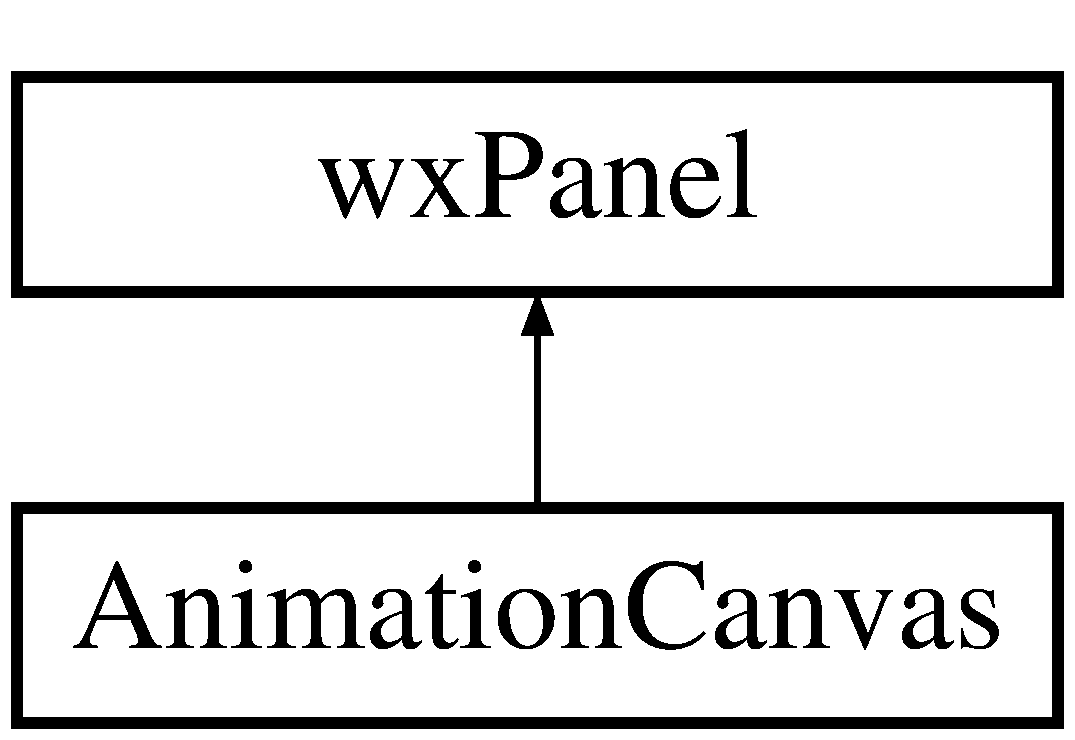
\includegraphics[height=2.000000cm]{a00011}
\end{center}
\end{figure}
\subsection*{Public Member Functions}
\begin{DoxyCompactItemize}
\item 
\hyperlink{a00011_a27fd0a655037468e01fc0921567508ad}{Animation\-Canvas} (\hyperlink{a00015}{Animation\-View} $\ast$view, wx\-Window $\ast$parent, const wx\-Size \&size=wx\-Default\-Size)
\item 
\hyperlink{a00011_a4623160539fb0844e62d3e3387448c37}{$\sim$\-Animation\-Canvas} ()
\item 
void \hyperlink{a00011_a2a7a367926dd5bb9480cb5d2c7c7051a}{Set\-View} (\hyperlink{a00015}{Animation\-View} $\ast$view)
\item 
void \hyperlink{a00011_ad31258b078d36ca77a25ac327b904763}{On\-Paint} (wx\-Paint\-Event \&event)
\item 
void \hyperlink{a00011_a4389c874d900e409a058edc610cfacab}{On\-Size} (wx\-Size\-Event \&event)
\item 
void \hyperlink{a00011_aac6118fb7d0b16cd22f22e4ff47e6808}{On\-Left\-Down\-Mouse\-Event} (wx\-Mouse\-Event \&event)
\item 
void \hyperlink{a00011_a88d8b515a238f35c1b0cf41d337a83cc}{On\-Left\-Up\-Mouse\-Event} (wx\-Mouse\-Event \&event)
\item 
void \hyperlink{a00011_a789939934f8342c5caab364340e9600e}{On\-Right\-Up\-Mouse\-Event} (wx\-Mouse\-Event \&event)
\item 
void \hyperlink{a00011_a162bd79a30723c1b670fdcbf1d64cc72}{On\-Mouse\-Move} (wx\-Mouse\-Event \&event)
\item 
void \hyperlink{a00011_a09028dec5a9f25f5e3c23df07c4e58c7}{On\-Char} (wx\-Key\-Event \&event)
\end{DoxyCompactItemize}
\subsection*{Private Member Functions}
\begin{DoxyCompactItemize}
\item 
\hyperlink{a00011_ae41a34ccada4a27315448a1e8d3d81a0}{wx\-D\-E\-C\-L\-A\-R\-E\-\_\-\-E\-V\-E\-N\-T\-\_\-\-T\-A\-B\-L\-E} ()
\end{DoxyCompactItemize}
\subsection*{Static Private Member Functions}
\begin{DoxyCompactItemize}
\item 
static float \hyperlink{a00011_a1f96260bb91404a7cc56bdbc516490bf}{Calc\-User\-Scale} (const \hyperlink{a00029}{C\-C\-\_\-coord} \&show\-Size, const wx\-Size \&window\-Size)
\item 
static wx\-Coord \hyperlink{a00011_a14a79bb267db01c136370a1593fabe9c}{Calc\-User\-Origin\-X} (const \hyperlink{a00029}{C\-C\-\_\-coord} \&show\-Size, const wx\-Size \&window\-Size)
\end{DoxyCompactItemize}
\subsection*{Private Attributes}
\begin{DoxyCompactItemize}
\item 
\hyperlink{a00015}{Animation\-View} $\ast$ \hyperlink{a00011_ad942e2dec46489d2a7c2783d807dde50}{m\-Animation\-View}
\item 
float \hyperlink{a00011_ab2f7205a34a828219d20e19d5d035804}{m\-User\-Scale}
\item 
wx\-Coord \hyperlink{a00011_aab7e581755be241f33566dae39b7737f}{m\-User\-Origin\-X}
\item 
bool \hyperlink{a00011_ace603466b0a8ced6e3258a8657c56c4c}{m\-Mouse\-Down}
\item 
long \hyperlink{a00011_a1274fba3c24501db2e78c8304a05b5f4}{m\-Mouse\-X\-Start}
\item 
long \hyperlink{a00011_a21bb228cd51fecf39cae7064b5668486}{m\-Mouse\-Y\-Start}
\item 
long \hyperlink{a00011_abb8fdd6f6c448b6a9c899b1bded98808}{m\-Mouse\-X\-End}
\item 
long \hyperlink{a00011_a502c5a9601e4355fb7f6fc69c357ce83}{m\-Mouse\-Y\-End}
\end{DoxyCompactItemize}
\subsection*{Static Private Attributes}
\begin{DoxyCompactItemize}
\item 
static const size\-\_\-t \hyperlink{a00011_ad96e4aae900ce990479cc9055638e932}{k\-Default\-Anim\-Size} = 3
\end{DoxyCompactItemize}


\subsection{Constructor \& Destructor Documentation}
\hypertarget{a00011_a27fd0a655037468e01fc0921567508ad}{\index{Animation\-Canvas@{Animation\-Canvas}!Animation\-Canvas@{Animation\-Canvas}}
\index{Animation\-Canvas@{Animation\-Canvas}!AnimationCanvas@{Animation\-Canvas}}
\subsubsection[{Animation\-Canvas}]{\setlength{\rightskip}{0pt plus 5cm}Animation\-Canvas\-::\-Animation\-Canvas (
\begin{DoxyParamCaption}
\item[{{\bf Animation\-View} $\ast$}]{view, }
\item[{wx\-Window $\ast$}]{parent, }
\item[{const wx\-Size \&}]{size = {\ttfamily wxDefaultSize}}
\end{DoxyParamCaption}
)}}\label{a00011_a27fd0a655037468e01fc0921567508ad}
\hypertarget{a00011_a4623160539fb0844e62d3e3387448c37}{\index{Animation\-Canvas@{Animation\-Canvas}!$\sim$\-Animation\-Canvas@{$\sim$\-Animation\-Canvas}}
\index{$\sim$\-Animation\-Canvas@{$\sim$\-Animation\-Canvas}!AnimationCanvas@{Animation\-Canvas}}
\subsubsection[{$\sim$\-Animation\-Canvas}]{\setlength{\rightskip}{0pt plus 5cm}Animation\-Canvas\-::$\sim$\-Animation\-Canvas (
\begin{DoxyParamCaption}
{}
\end{DoxyParamCaption}
)}}\label{a00011_a4623160539fb0844e62d3e3387448c37}


\subsection{Member Function Documentation}
\hypertarget{a00011_a14a79bb267db01c136370a1593fabe9c}{\index{Animation\-Canvas@{Animation\-Canvas}!Calc\-User\-Origin\-X@{Calc\-User\-Origin\-X}}
\index{Calc\-User\-Origin\-X@{Calc\-User\-Origin\-X}!AnimationCanvas@{Animation\-Canvas}}
\subsubsection[{Calc\-User\-Origin\-X}]{\setlength{\rightskip}{0pt plus 5cm}wx\-Coord Animation\-Canvas\-::\-Calc\-User\-Origin\-X (
\begin{DoxyParamCaption}
\item[{const {\bf C\-C\-\_\-coord} \&}]{show\-Size, }
\item[{const wx\-Size \&}]{window\-Size}
\end{DoxyParamCaption}
)\hspace{0.3cm}{\ttfamily [static]}, {\ttfamily [private]}}}\label{a00011_a14a79bb267db01c136370a1593fabe9c}
\hypertarget{a00011_a1f96260bb91404a7cc56bdbc516490bf}{\index{Animation\-Canvas@{Animation\-Canvas}!Calc\-User\-Scale@{Calc\-User\-Scale}}
\index{Calc\-User\-Scale@{Calc\-User\-Scale}!AnimationCanvas@{Animation\-Canvas}}
\subsubsection[{Calc\-User\-Scale}]{\setlength{\rightskip}{0pt plus 5cm}float Animation\-Canvas\-::\-Calc\-User\-Scale (
\begin{DoxyParamCaption}
\item[{const {\bf C\-C\-\_\-coord} \&}]{show\-Size, }
\item[{const wx\-Size \&}]{window\-Size}
\end{DoxyParamCaption}
)\hspace{0.3cm}{\ttfamily [static]}, {\ttfamily [private]}}}\label{a00011_a1f96260bb91404a7cc56bdbc516490bf}
\hypertarget{a00011_a09028dec5a9f25f5e3c23df07c4e58c7}{\index{Animation\-Canvas@{Animation\-Canvas}!On\-Char@{On\-Char}}
\index{On\-Char@{On\-Char}!AnimationCanvas@{Animation\-Canvas}}
\subsubsection[{On\-Char}]{\setlength{\rightskip}{0pt plus 5cm}void Animation\-Canvas\-::\-On\-Char (
\begin{DoxyParamCaption}
\item[{wx\-Key\-Event \&}]{event}
\end{DoxyParamCaption}
)}}\label{a00011_a09028dec5a9f25f5e3c23df07c4e58c7}
\hypertarget{a00011_aac6118fb7d0b16cd22f22e4ff47e6808}{\index{Animation\-Canvas@{Animation\-Canvas}!On\-Left\-Down\-Mouse\-Event@{On\-Left\-Down\-Mouse\-Event}}
\index{On\-Left\-Down\-Mouse\-Event@{On\-Left\-Down\-Mouse\-Event}!AnimationCanvas@{Animation\-Canvas}}
\subsubsection[{On\-Left\-Down\-Mouse\-Event}]{\setlength{\rightskip}{0pt plus 5cm}void Animation\-Canvas\-::\-On\-Left\-Down\-Mouse\-Event (
\begin{DoxyParamCaption}
\item[{wx\-Mouse\-Event \&}]{event}
\end{DoxyParamCaption}
)}}\label{a00011_aac6118fb7d0b16cd22f22e4ff47e6808}
\hypertarget{a00011_a88d8b515a238f35c1b0cf41d337a83cc}{\index{Animation\-Canvas@{Animation\-Canvas}!On\-Left\-Up\-Mouse\-Event@{On\-Left\-Up\-Mouse\-Event}}
\index{On\-Left\-Up\-Mouse\-Event@{On\-Left\-Up\-Mouse\-Event}!AnimationCanvas@{Animation\-Canvas}}
\subsubsection[{On\-Left\-Up\-Mouse\-Event}]{\setlength{\rightskip}{0pt plus 5cm}void Animation\-Canvas\-::\-On\-Left\-Up\-Mouse\-Event (
\begin{DoxyParamCaption}
\item[{wx\-Mouse\-Event \&}]{event}
\end{DoxyParamCaption}
)}}\label{a00011_a88d8b515a238f35c1b0cf41d337a83cc}
\hypertarget{a00011_a162bd79a30723c1b670fdcbf1d64cc72}{\index{Animation\-Canvas@{Animation\-Canvas}!On\-Mouse\-Move@{On\-Mouse\-Move}}
\index{On\-Mouse\-Move@{On\-Mouse\-Move}!AnimationCanvas@{Animation\-Canvas}}
\subsubsection[{On\-Mouse\-Move}]{\setlength{\rightskip}{0pt plus 5cm}void Animation\-Canvas\-::\-On\-Mouse\-Move (
\begin{DoxyParamCaption}
\item[{wx\-Mouse\-Event \&}]{event}
\end{DoxyParamCaption}
)}}\label{a00011_a162bd79a30723c1b670fdcbf1d64cc72}
\hypertarget{a00011_ad31258b078d36ca77a25ac327b904763}{\index{Animation\-Canvas@{Animation\-Canvas}!On\-Paint@{On\-Paint}}
\index{On\-Paint@{On\-Paint}!AnimationCanvas@{Animation\-Canvas}}
\subsubsection[{On\-Paint}]{\setlength{\rightskip}{0pt plus 5cm}void Animation\-Canvas\-::\-On\-Paint (
\begin{DoxyParamCaption}
\item[{wx\-Paint\-Event \&}]{event}
\end{DoxyParamCaption}
)}}\label{a00011_ad31258b078d36ca77a25ac327b904763}
\hypertarget{a00011_a789939934f8342c5caab364340e9600e}{\index{Animation\-Canvas@{Animation\-Canvas}!On\-Right\-Up\-Mouse\-Event@{On\-Right\-Up\-Mouse\-Event}}
\index{On\-Right\-Up\-Mouse\-Event@{On\-Right\-Up\-Mouse\-Event}!AnimationCanvas@{Animation\-Canvas}}
\subsubsection[{On\-Right\-Up\-Mouse\-Event}]{\setlength{\rightskip}{0pt plus 5cm}void Animation\-Canvas\-::\-On\-Right\-Up\-Mouse\-Event (
\begin{DoxyParamCaption}
\item[{wx\-Mouse\-Event \&}]{event}
\end{DoxyParamCaption}
)}}\label{a00011_a789939934f8342c5caab364340e9600e}
\hypertarget{a00011_a4389c874d900e409a058edc610cfacab}{\index{Animation\-Canvas@{Animation\-Canvas}!On\-Size@{On\-Size}}
\index{On\-Size@{On\-Size}!AnimationCanvas@{Animation\-Canvas}}
\subsubsection[{On\-Size}]{\setlength{\rightskip}{0pt plus 5cm}void Animation\-Canvas\-::\-On\-Size (
\begin{DoxyParamCaption}
\item[{wx\-Size\-Event \&}]{event}
\end{DoxyParamCaption}
)}}\label{a00011_a4389c874d900e409a058edc610cfacab}
\hypertarget{a00011_a2a7a367926dd5bb9480cb5d2c7c7051a}{\index{Animation\-Canvas@{Animation\-Canvas}!Set\-View@{Set\-View}}
\index{Set\-View@{Set\-View}!AnimationCanvas@{Animation\-Canvas}}
\subsubsection[{Set\-View}]{\setlength{\rightskip}{0pt plus 5cm}void Animation\-Canvas\-::\-Set\-View (
\begin{DoxyParamCaption}
\item[{{\bf Animation\-View} $\ast$}]{view}
\end{DoxyParamCaption}
)}}\label{a00011_a2a7a367926dd5bb9480cb5d2c7c7051a}
\hypertarget{a00011_ae41a34ccada4a27315448a1e8d3d81a0}{\index{Animation\-Canvas@{Animation\-Canvas}!wx\-D\-E\-C\-L\-A\-R\-E\-\_\-\-E\-V\-E\-N\-T\-\_\-\-T\-A\-B\-L\-E@{wx\-D\-E\-C\-L\-A\-R\-E\-\_\-\-E\-V\-E\-N\-T\-\_\-\-T\-A\-B\-L\-E}}
\index{wx\-D\-E\-C\-L\-A\-R\-E\-\_\-\-E\-V\-E\-N\-T\-\_\-\-T\-A\-B\-L\-E@{wx\-D\-E\-C\-L\-A\-R\-E\-\_\-\-E\-V\-E\-N\-T\-\_\-\-T\-A\-B\-L\-E}!AnimationCanvas@{Animation\-Canvas}}
\subsubsection[{wx\-D\-E\-C\-L\-A\-R\-E\-\_\-\-E\-V\-E\-N\-T\-\_\-\-T\-A\-B\-L\-E}]{\setlength{\rightskip}{0pt plus 5cm}Animation\-Canvas\-::wx\-D\-E\-C\-L\-A\-R\-E\-\_\-\-E\-V\-E\-N\-T\-\_\-\-T\-A\-B\-L\-E (
\begin{DoxyParamCaption}
{}
\end{DoxyParamCaption}
)\hspace{0.3cm}{\ttfamily [private]}}}\label{a00011_ae41a34ccada4a27315448a1e8d3d81a0}


\subsection{Member Data Documentation}
\hypertarget{a00011_ad96e4aae900ce990479cc9055638e932}{\index{Animation\-Canvas@{Animation\-Canvas}!k\-Default\-Anim\-Size@{k\-Default\-Anim\-Size}}
\index{k\-Default\-Anim\-Size@{k\-Default\-Anim\-Size}!AnimationCanvas@{Animation\-Canvas}}
\subsubsection[{k\-Default\-Anim\-Size}]{\setlength{\rightskip}{0pt plus 5cm}const size\-\_\-t Animation\-Canvas\-::k\-Default\-Anim\-Size = 3\hspace{0.3cm}{\ttfamily [static]}, {\ttfamily [private]}}}\label{a00011_ad96e4aae900ce990479cc9055638e932}
\hypertarget{a00011_ad942e2dec46489d2a7c2783d807dde50}{\index{Animation\-Canvas@{Animation\-Canvas}!m\-Animation\-View@{m\-Animation\-View}}
\index{m\-Animation\-View@{m\-Animation\-View}!AnimationCanvas@{Animation\-Canvas}}
\subsubsection[{m\-Animation\-View}]{\setlength{\rightskip}{0pt plus 5cm}{\bf Animation\-View}$\ast$ Animation\-Canvas\-::m\-Animation\-View\hspace{0.3cm}{\ttfamily [private]}}}\label{a00011_ad942e2dec46489d2a7c2783d807dde50}
\hypertarget{a00011_ace603466b0a8ced6e3258a8657c56c4c}{\index{Animation\-Canvas@{Animation\-Canvas}!m\-Mouse\-Down@{m\-Mouse\-Down}}
\index{m\-Mouse\-Down@{m\-Mouse\-Down}!AnimationCanvas@{Animation\-Canvas}}
\subsubsection[{m\-Mouse\-Down}]{\setlength{\rightskip}{0pt plus 5cm}bool Animation\-Canvas\-::m\-Mouse\-Down\hspace{0.3cm}{\ttfamily [private]}}}\label{a00011_ace603466b0a8ced6e3258a8657c56c4c}
\hypertarget{a00011_abb8fdd6f6c448b6a9c899b1bded98808}{\index{Animation\-Canvas@{Animation\-Canvas}!m\-Mouse\-X\-End@{m\-Mouse\-X\-End}}
\index{m\-Mouse\-X\-End@{m\-Mouse\-X\-End}!AnimationCanvas@{Animation\-Canvas}}
\subsubsection[{m\-Mouse\-X\-End}]{\setlength{\rightskip}{0pt plus 5cm}long Animation\-Canvas\-::m\-Mouse\-X\-End\hspace{0.3cm}{\ttfamily [private]}}}\label{a00011_abb8fdd6f6c448b6a9c899b1bded98808}
\hypertarget{a00011_a1274fba3c24501db2e78c8304a05b5f4}{\index{Animation\-Canvas@{Animation\-Canvas}!m\-Mouse\-X\-Start@{m\-Mouse\-X\-Start}}
\index{m\-Mouse\-X\-Start@{m\-Mouse\-X\-Start}!AnimationCanvas@{Animation\-Canvas}}
\subsubsection[{m\-Mouse\-X\-Start}]{\setlength{\rightskip}{0pt plus 5cm}long Animation\-Canvas\-::m\-Mouse\-X\-Start\hspace{0.3cm}{\ttfamily [private]}}}\label{a00011_a1274fba3c24501db2e78c8304a05b5f4}
\hypertarget{a00011_a502c5a9601e4355fb7f6fc69c357ce83}{\index{Animation\-Canvas@{Animation\-Canvas}!m\-Mouse\-Y\-End@{m\-Mouse\-Y\-End}}
\index{m\-Mouse\-Y\-End@{m\-Mouse\-Y\-End}!AnimationCanvas@{Animation\-Canvas}}
\subsubsection[{m\-Mouse\-Y\-End}]{\setlength{\rightskip}{0pt plus 5cm}long Animation\-Canvas\-::m\-Mouse\-Y\-End\hspace{0.3cm}{\ttfamily [private]}}}\label{a00011_a502c5a9601e4355fb7f6fc69c357ce83}
\hypertarget{a00011_a21bb228cd51fecf39cae7064b5668486}{\index{Animation\-Canvas@{Animation\-Canvas}!m\-Mouse\-Y\-Start@{m\-Mouse\-Y\-Start}}
\index{m\-Mouse\-Y\-Start@{m\-Mouse\-Y\-Start}!AnimationCanvas@{Animation\-Canvas}}
\subsubsection[{m\-Mouse\-Y\-Start}]{\setlength{\rightskip}{0pt plus 5cm}long Animation\-Canvas\-::m\-Mouse\-Y\-Start\hspace{0.3cm}{\ttfamily [private]}}}\label{a00011_a21bb228cd51fecf39cae7064b5668486}
\hypertarget{a00011_aab7e581755be241f33566dae39b7737f}{\index{Animation\-Canvas@{Animation\-Canvas}!m\-User\-Origin\-X@{m\-User\-Origin\-X}}
\index{m\-User\-Origin\-X@{m\-User\-Origin\-X}!AnimationCanvas@{Animation\-Canvas}}
\subsubsection[{m\-User\-Origin\-X}]{\setlength{\rightskip}{0pt plus 5cm}wx\-Coord Animation\-Canvas\-::m\-User\-Origin\-X\hspace{0.3cm}{\ttfamily [private]}}}\label{a00011_aab7e581755be241f33566dae39b7737f}
\hypertarget{a00011_ab2f7205a34a828219d20e19d5d035804}{\index{Animation\-Canvas@{Animation\-Canvas}!m\-User\-Scale@{m\-User\-Scale}}
\index{m\-User\-Scale@{m\-User\-Scale}!AnimationCanvas@{Animation\-Canvas}}
\subsubsection[{m\-User\-Scale}]{\setlength{\rightskip}{0pt plus 5cm}float Animation\-Canvas\-::m\-User\-Scale\hspace{0.3cm}{\ttfamily [private]}}}\label{a00011_ab2f7205a34a828219d20e19d5d035804}


The documentation for this class was generated from the following files\-:\begin{DoxyCompactItemize}
\item 
src/\hyperlink{a00169}{animation\-\_\-canvas.\-h}\item 
src/\hyperlink{a00168}{animation\-\_\-canvas.\-cpp}\end{DoxyCompactItemize}

\hypertarget{a00012}{\section{Animation\-Frame Class Reference}
\label{a00012}\index{Animation\-Frame@{Animation\-Frame}}
}


{\ttfamily \#include $<$animation\-\_\-frame.\-h$>$}

Inheritance diagram for Animation\-Frame\-:\begin{figure}[H]
\begin{center}
\leavevmode
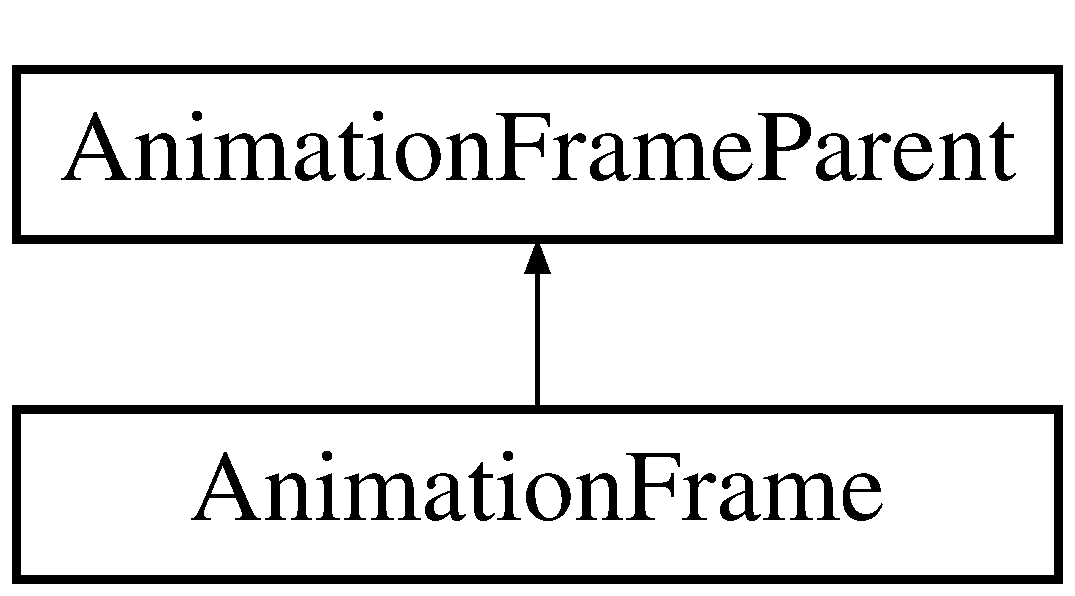
\includegraphics[height=2.000000cm]{a00012}
\end{center}
\end{figure}
\subsection*{Public Types}
\begin{DoxyCompactItemize}
\item 
typedef \hyperlink{a00171_a8b295c639a8d2391dc4584107c78db16}{Animation\-Frame\-Parent} \hyperlink{a00012_a090eb07704cc6d7005dc5cd99da6d8bd}{super}
\end{DoxyCompactItemize}
\subsection*{Public Member Functions}
\begin{DoxyCompactItemize}
\item 
\hyperlink{a00012_a6f09b3d61b3daba0da8c3db0d76f0c9f}{Animation\-Frame} (boost\-::function$<$ void()$>$ on\-Close, wx\-Document $\ast$doc, wx\-View $\ast$view, wx\-Frame $\ast$parent, const wx\-Size \&size)
\item 
\hyperlink{a00012_af9da581313899adf881d6c1578cfa198}{$\sim$\-Animation\-Frame} ()
\item 
void \hyperlink{a00012_af77a9a0455fdb7a9e920c470a62e4892}{On\-Size} (wx\-Size\-Event \&event)
\item 
void \hyperlink{a00012_ae881dcbe9ae16c43aa2a3bdd78d7c826}{On\-Cmd\-Reanimate} (wx\-Command\-Event \&event)
\item 
void \hyperlink{a00012_ab8b90e1808b3873ddaed5c9e6210e21c}{On\-Cmd\-Select\-Collisions} (wx\-Command\-Event \&event)
\item 
void \hyperlink{a00012_a294a28e405a98129330f8e6d08bc863d}{On\-Cmd\-Close} (wx\-Command\-Event \&event)
\item 
void \hyperlink{a00012_aff7e18668d20664ce886829dc9849545}{On\-Cmd\-Close} (wx\-Close\-Event \&event)
\item 
void \hyperlink{a00012_a8afdb773f9dcb3048dac535ff170f1c3}{On\-Cmd\-\_\-anim\-\_\-stop} (wx\-Command\-Event \&event)
\item 
void \hyperlink{a00012_a79a27795f5e0327a93ae364af06608dc}{On\-Cmd\-\_\-anim\-\_\-play} (wx\-Command\-Event \&event)
\item 
void \hyperlink{a00012_a9571d8ba4321295994befdb087ac918b}{On\-Cmd\-\_\-anim\-\_\-prev\-\_\-beat} (wx\-Command\-Event \&event)
\item 
void \hyperlink{a00012_a59a91e0ab85132e7006d8b09a304162f}{On\-Cmd\-\_\-anim\-\_\-next\-\_\-beat} (wx\-Command\-Event \&event)
\item 
void \hyperlink{a00012_a1fbe1fb265f8cd92089f5db7564c571b}{On\-Cmd\-\_\-anim\-\_\-next\-\_\-beat\-\_\-timer} (wx\-Timer\-Event \&event)
\item 
void \hyperlink{a00012_adb11edc49b4894f0d44be0e4ca19dd02}{On\-Cmd\-\_\-anim\-\_\-prev\-\_\-sheet} (wx\-Command\-Event \&event)
\item 
void \hyperlink{a00012_a0ddd320c42cabac2cc297a38fd472c5c}{On\-Cmd\-\_\-anim\-\_\-next\-\_\-sheet} (wx\-Command\-Event \&event)
\item 
void \hyperlink{a00012_a66522efb1ba929091b007847d5731062}{On\-Cmd\-\_\-anim\-\_\-collisions} (wx\-Command\-Event \&event)
\item 
void \hyperlink{a00012_a6b92abad4cb4de31486819b52324a220}{On\-Cmd\-\_\-anim\-\_\-errors} (wx\-Command\-Event \&event)
\item 
void \hyperlink{a00012_a5ba62cdbffd7d38267afd247b392177e}{On\-Slider\-\_\-anim\-\_\-tempo} (wx\-Spin\-Event \&event)
\item 
void \hyperlink{a00012_a00bcedee9639a6cdfe6d5b155decce7e}{On\-Slider\-\_\-anim\-\_\-gotosheet} (wx\-Scroll\-Event \&event)
\item 
void \hyperlink{a00012_ae856b335a3ae8d693009289dfb81ab2f}{On\-Slider\-\_\-anim\-\_\-gotobeat} (wx\-Scroll\-Event \&event)
\item 
void \hyperlink{a00012_a1371542268ed553069f757400326c6f6}{On\-Cmd\-\_\-\-Follow\-Marcher} (wx\-Command\-Event \&event)
\item 
void \hyperlink{a00012_a535bf369a05e55e151dbf35d4c8730b6}{On\-Cmd\-\_\-\-Save\-Camera\-Angle} (wx\-Command\-Event \&event)
\item 
void \hyperlink{a00012_a491228762f2739e53ee796551aa05e73}{On\-Cmd\-\_\-\-Go\-To\-Camera\-Angle} (wx\-Command\-Event \&event)
\item 
void \hyperlink{a00012_ac559d77663e583937a44506f1c06aa75}{On\-Cmd\-\_\-\-Show\-Keyboard\-Controls} (wx\-Command\-Event \&event)
\item 
void \hyperlink{a00012_afe675f7081ca6a4352c5bcd2444e1fc3}{On\-Cmd\-\_\-\-Toggle\-Crowd} (wx\-Command\-Event \&event)
\item 
void \hyperlink{a00012_ab65c1e97af52af268606a76178cf64f5}{On\-Cmd\-\_\-\-Toggle\-Marching} (wx\-Command\-Event \&event)
\item 
void \hyperlink{a00012_aa1b1cfd58585f393ed022e2bcb4be71a}{On\-Cmd\-\_\-\-Toggle\-Show\-Only\-Selected} (wx\-Command\-Event \&event)
\item 
void \hyperlink{a00012_aa2be2a08b4ec5421f58a62447d55a788}{Toggle\-Timer} ()
\item 
void \hyperlink{a00012_aededa63d75a6afab9c85a1ba64d95ccb}{Update\-Panel} ()
\item 
bool \hyperlink{a00012_abb86dfea245b11389b7f28b054e786fb}{On\-Beat} () const 
\item 
void \hyperlink{a00012_a544275588f75eb702749983997b8843d}{On\-Notify\-Error\-List} (const std\-::vector$<$ \hyperlink{a00098}{Error\-Marker} $>$ \&error\-\_\-markers, unsigned sheetnum, const wx\-String \&message)
\item 
void \hyperlink{a00012_ab3b780fc7a2f4a5a9f446936e2b0048a}{On\-Cmd\-\_\-\-Split\-View\-Horizontal} (wx\-Command\-Event \&event)
\item 
void \hyperlink{a00012_a45e8fa52738d8d66fcc1b151827dc147}{On\-Cmd\-\_\-\-Split\-View\-Vertical} (wx\-Command\-Event \&event)
\item 
void \hyperlink{a00012_aea1520c2384b56db2168c9e505a9a112}{On\-Cmd\-\_\-\-Split\-View\-Unsplit} (wx\-Command\-Event \&event)
\item 
void \hyperlink{a00012_a6d4a2c6c42801aae9aeea9d09f3dc2a0}{On\-Cmd\-\_\-\-Swap\-Animate\-And\-Omni} (wx\-Command\-Event \&event)
\item 
void \hyperlink{a00012_ac0245ddc2c39c08607a589fcc4144e42}{On\-Cmd\-\_\-\-Update\-U\-I\-Horizontal} (wx\-Update\-U\-I\-Event \&event)
\item 
void \hyperlink{a00012_ae19ce9d9595299a042e419de06029c29}{On\-Cmd\-\_\-\-Update\-U\-I\-Vertical} (wx\-Update\-U\-I\-Event \&event)
\item 
void \hyperlink{a00012_ad0733292c32be2844b8f8f87751f9ebf}{On\-Cmd\-\_\-\-Update\-U\-I\-Unsplit} (wx\-Update\-U\-I\-Event \&event)
\end{DoxyCompactItemize}
\subsection*{Private Member Functions}
\begin{DoxyCompactItemize}
\item 
void \hyperlink{a00012_a36ab818a3dd8bc80d781aac236b0d05f}{Start\-Timer} ()
\item 
void \hyperlink{a00012_add918ea87055d1c9ea2cb1b50cea86ff}{Stop\-Timer} ()
\item 
unsigned \hyperlink{a00012_a931add98a5ce97799285d89ddcbcb952}{Get\-Tempo} () const 
\item 
void \hyperlink{a00012_a1786641595eeb2b37b7f9094d7082a99}{Set\-Tempo} (unsigned tempo)
\item 
\hyperlink{a00012_a3942acc9c6a4d49ff2ceb9bbccd3c404}{wx\-D\-E\-C\-L\-A\-R\-E\-\_\-\-E\-V\-E\-N\-T\-\_\-\-T\-A\-B\-L\-E} ()
\end{DoxyCompactItemize}
\subsection*{Private Attributes}
\begin{DoxyCompactItemize}
\item 
\hyperlink{a00015}{Animation\-View} $\ast$ \hyperlink{a00012_a8eaf0667f46fd0a32d400513fc0dbe6f}{m\-Animation\-View}
\item 
\hyperlink{a00011}{Animation\-Canvas} $\ast$ \hyperlink{a00012_a6b272e1e5149c0852be68df793d91319}{m\-Canvas}
\item 
\hyperlink{a00049}{C\-C\-Omni\-View\-\_\-\-Canvas} $\ast$ \hyperlink{a00012_a5aefb21e1f10427c4c39e57cba2bea9a}{m\-Omni\-View\-Canvas}
\item 
wx\-Slider $\ast$ \hyperlink{a00012_a24a43b9bb1c10f0b33d1ffaf6a8bbc0c}{m\-Sheet\-Slider}
\item 
wx\-Slider $\ast$ \hyperlink{a00012_a88521e7acd54e1b979933cea349093a5}{m\-Beat\-Slider}
\item 
wx\-Splitter\-Window $\ast$ \hyperlink{a00012_a0834dc7f3ff34dea334cf0c1d6bf5333}{m\-Splitter}
\item 
wx\-Window $\ast$ \hyperlink{a00012_aaf2b976d3be7e9c01fd011349933506a}{m\-Split\-A}
\item 
wx\-Window $\ast$ \hyperlink{a00012_af4f663056a3e3452d154976cf4674a92}{m\-Split\-B}
\item 
wx\-Choice $\ast$ \hyperlink{a00012_af7449f029e00d8a7865dca8a2e89674f}{m\-Error\-List}
\item 
std\-::vector$<$ std\-::pair\\*
$<$ \hyperlink{a00098}{Error\-Marker}, unsigned $>$ $>$ \hyperlink{a00012_a9e3504eaefd868db5e1cf25b68e4c164}{m\-Error\-Markers}
\item 
\hyperlink{a00099}{Fancy\-Text\-Win} $\ast$ \hyperlink{a00012_a9afe128fc249c04a4b77a3ebffc0e922}{m\-Error\-Text}
\item 
wx\-Timer $\ast$ \hyperlink{a00012_aa48d3d2e5cd0c3d39153cdc8b1581994}{m\-Timer}
\item 
unsigned \hyperlink{a00012_a192f6bee3cbd7e25c9d64b34e605decd}{m\-Tempo}
\item 
bool \hyperlink{a00012_a73516f06167cd8f8cb18d6d9c213196f}{m\-Timer\-On}
\item 
boost\-::function$<$ void()$>$ \hyperlink{a00012_aceadfa02d59d86be954eda1e69245465}{m\-When\-Closed}
\end{DoxyCompactItemize}


\subsection{Member Typedef Documentation}
\hypertarget{a00012_a090eb07704cc6d7005dc5cd99da6d8bd}{\index{Animation\-Frame@{Animation\-Frame}!super@{super}}
\index{super@{super}!AnimationFrame@{Animation\-Frame}}
\subsubsection[{super}]{\setlength{\rightskip}{0pt plus 5cm}typedef {\bf Animation\-Frame\-Parent} {\bf Animation\-Frame\-::super}}}\label{a00012_a090eb07704cc6d7005dc5cd99da6d8bd}


\subsection{Constructor \& Destructor Documentation}
\hypertarget{a00012_a6f09b3d61b3daba0da8c3db0d76f0c9f}{\index{Animation\-Frame@{Animation\-Frame}!Animation\-Frame@{Animation\-Frame}}
\index{Animation\-Frame@{Animation\-Frame}!AnimationFrame@{Animation\-Frame}}
\subsubsection[{Animation\-Frame}]{\setlength{\rightskip}{0pt plus 5cm}Animation\-Frame\-::\-Animation\-Frame (
\begin{DoxyParamCaption}
\item[{boost\-::function$<$ void()$>$}]{on\-Close, }
\item[{wx\-Document $\ast$}]{doc, }
\item[{wx\-View $\ast$}]{view, }
\item[{wx\-Frame $\ast$}]{parent, }
\item[{const wx\-Size \&}]{size}
\end{DoxyParamCaption}
)}}\label{a00012_a6f09b3d61b3daba0da8c3db0d76f0c9f}
\hypertarget{a00012_af9da581313899adf881d6c1578cfa198}{\index{Animation\-Frame@{Animation\-Frame}!$\sim$\-Animation\-Frame@{$\sim$\-Animation\-Frame}}
\index{$\sim$\-Animation\-Frame@{$\sim$\-Animation\-Frame}!AnimationFrame@{Animation\-Frame}}
\subsubsection[{$\sim$\-Animation\-Frame}]{\setlength{\rightskip}{0pt plus 5cm}Animation\-Frame\-::$\sim$\-Animation\-Frame (
\begin{DoxyParamCaption}
{}
\end{DoxyParamCaption}
)}}\label{a00012_af9da581313899adf881d6c1578cfa198}


\subsection{Member Function Documentation}
\hypertarget{a00012_a931add98a5ce97799285d89ddcbcb952}{\index{Animation\-Frame@{Animation\-Frame}!Get\-Tempo@{Get\-Tempo}}
\index{Get\-Tempo@{Get\-Tempo}!AnimationFrame@{Animation\-Frame}}
\subsubsection[{Get\-Tempo}]{\setlength{\rightskip}{0pt plus 5cm}unsigned Animation\-Frame\-::\-Get\-Tempo (
\begin{DoxyParamCaption}
{}
\end{DoxyParamCaption}
) const\hspace{0.3cm}{\ttfamily [private]}}}\label{a00012_a931add98a5ce97799285d89ddcbcb952}
\hypertarget{a00012_abb86dfea245b11389b7f28b054e786fb}{\index{Animation\-Frame@{Animation\-Frame}!On\-Beat@{On\-Beat}}
\index{On\-Beat@{On\-Beat}!AnimationFrame@{Animation\-Frame}}
\subsubsection[{On\-Beat}]{\setlength{\rightskip}{0pt plus 5cm}bool Animation\-Frame\-::\-On\-Beat (
\begin{DoxyParamCaption}
{}
\end{DoxyParamCaption}
) const}}\label{a00012_abb86dfea245b11389b7f28b054e786fb}
\hypertarget{a00012_a66522efb1ba929091b007847d5731062}{\index{Animation\-Frame@{Animation\-Frame}!On\-Cmd\-\_\-anim\-\_\-collisions@{On\-Cmd\-\_\-anim\-\_\-collisions}}
\index{On\-Cmd\-\_\-anim\-\_\-collisions@{On\-Cmd\-\_\-anim\-\_\-collisions}!AnimationFrame@{Animation\-Frame}}
\subsubsection[{On\-Cmd\-\_\-anim\-\_\-collisions}]{\setlength{\rightskip}{0pt plus 5cm}void Animation\-Frame\-::\-On\-Cmd\-\_\-anim\-\_\-collisions (
\begin{DoxyParamCaption}
\item[{wx\-Command\-Event \&}]{event}
\end{DoxyParamCaption}
)}}\label{a00012_a66522efb1ba929091b007847d5731062}
\hypertarget{a00012_a6b92abad4cb4de31486819b52324a220}{\index{Animation\-Frame@{Animation\-Frame}!On\-Cmd\-\_\-anim\-\_\-errors@{On\-Cmd\-\_\-anim\-\_\-errors}}
\index{On\-Cmd\-\_\-anim\-\_\-errors@{On\-Cmd\-\_\-anim\-\_\-errors}!AnimationFrame@{Animation\-Frame}}
\subsubsection[{On\-Cmd\-\_\-anim\-\_\-errors}]{\setlength{\rightskip}{0pt plus 5cm}void Animation\-Frame\-::\-On\-Cmd\-\_\-anim\-\_\-errors (
\begin{DoxyParamCaption}
\item[{wx\-Command\-Event \&}]{event}
\end{DoxyParamCaption}
)}}\label{a00012_a6b92abad4cb4de31486819b52324a220}
\hypertarget{a00012_a59a91e0ab85132e7006d8b09a304162f}{\index{Animation\-Frame@{Animation\-Frame}!On\-Cmd\-\_\-anim\-\_\-next\-\_\-beat@{On\-Cmd\-\_\-anim\-\_\-next\-\_\-beat}}
\index{On\-Cmd\-\_\-anim\-\_\-next\-\_\-beat@{On\-Cmd\-\_\-anim\-\_\-next\-\_\-beat}!AnimationFrame@{Animation\-Frame}}
\subsubsection[{On\-Cmd\-\_\-anim\-\_\-next\-\_\-beat}]{\setlength{\rightskip}{0pt plus 5cm}void Animation\-Frame\-::\-On\-Cmd\-\_\-anim\-\_\-next\-\_\-beat (
\begin{DoxyParamCaption}
\item[{wx\-Command\-Event \&}]{event}
\end{DoxyParamCaption}
)}}\label{a00012_a59a91e0ab85132e7006d8b09a304162f}
\hypertarget{a00012_a1fbe1fb265f8cd92089f5db7564c571b}{\index{Animation\-Frame@{Animation\-Frame}!On\-Cmd\-\_\-anim\-\_\-next\-\_\-beat\-\_\-timer@{On\-Cmd\-\_\-anim\-\_\-next\-\_\-beat\-\_\-timer}}
\index{On\-Cmd\-\_\-anim\-\_\-next\-\_\-beat\-\_\-timer@{On\-Cmd\-\_\-anim\-\_\-next\-\_\-beat\-\_\-timer}!AnimationFrame@{Animation\-Frame}}
\subsubsection[{On\-Cmd\-\_\-anim\-\_\-next\-\_\-beat\-\_\-timer}]{\setlength{\rightskip}{0pt plus 5cm}void Animation\-Frame\-::\-On\-Cmd\-\_\-anim\-\_\-next\-\_\-beat\-\_\-timer (
\begin{DoxyParamCaption}
\item[{wx\-Timer\-Event \&}]{event}
\end{DoxyParamCaption}
)}}\label{a00012_a1fbe1fb265f8cd92089f5db7564c571b}
\hypertarget{a00012_a0ddd320c42cabac2cc297a38fd472c5c}{\index{Animation\-Frame@{Animation\-Frame}!On\-Cmd\-\_\-anim\-\_\-next\-\_\-sheet@{On\-Cmd\-\_\-anim\-\_\-next\-\_\-sheet}}
\index{On\-Cmd\-\_\-anim\-\_\-next\-\_\-sheet@{On\-Cmd\-\_\-anim\-\_\-next\-\_\-sheet}!AnimationFrame@{Animation\-Frame}}
\subsubsection[{On\-Cmd\-\_\-anim\-\_\-next\-\_\-sheet}]{\setlength{\rightskip}{0pt plus 5cm}void Animation\-Frame\-::\-On\-Cmd\-\_\-anim\-\_\-next\-\_\-sheet (
\begin{DoxyParamCaption}
\item[{wx\-Command\-Event \&}]{event}
\end{DoxyParamCaption}
)}}\label{a00012_a0ddd320c42cabac2cc297a38fd472c5c}
\hypertarget{a00012_a79a27795f5e0327a93ae364af06608dc}{\index{Animation\-Frame@{Animation\-Frame}!On\-Cmd\-\_\-anim\-\_\-play@{On\-Cmd\-\_\-anim\-\_\-play}}
\index{On\-Cmd\-\_\-anim\-\_\-play@{On\-Cmd\-\_\-anim\-\_\-play}!AnimationFrame@{Animation\-Frame}}
\subsubsection[{On\-Cmd\-\_\-anim\-\_\-play}]{\setlength{\rightskip}{0pt plus 5cm}void Animation\-Frame\-::\-On\-Cmd\-\_\-anim\-\_\-play (
\begin{DoxyParamCaption}
\item[{wx\-Command\-Event \&}]{event}
\end{DoxyParamCaption}
)}}\label{a00012_a79a27795f5e0327a93ae364af06608dc}
\hypertarget{a00012_a9571d8ba4321295994befdb087ac918b}{\index{Animation\-Frame@{Animation\-Frame}!On\-Cmd\-\_\-anim\-\_\-prev\-\_\-beat@{On\-Cmd\-\_\-anim\-\_\-prev\-\_\-beat}}
\index{On\-Cmd\-\_\-anim\-\_\-prev\-\_\-beat@{On\-Cmd\-\_\-anim\-\_\-prev\-\_\-beat}!AnimationFrame@{Animation\-Frame}}
\subsubsection[{On\-Cmd\-\_\-anim\-\_\-prev\-\_\-beat}]{\setlength{\rightskip}{0pt plus 5cm}void Animation\-Frame\-::\-On\-Cmd\-\_\-anim\-\_\-prev\-\_\-beat (
\begin{DoxyParamCaption}
\item[{wx\-Command\-Event \&}]{event}
\end{DoxyParamCaption}
)}}\label{a00012_a9571d8ba4321295994befdb087ac918b}
\hypertarget{a00012_adb11edc49b4894f0d44be0e4ca19dd02}{\index{Animation\-Frame@{Animation\-Frame}!On\-Cmd\-\_\-anim\-\_\-prev\-\_\-sheet@{On\-Cmd\-\_\-anim\-\_\-prev\-\_\-sheet}}
\index{On\-Cmd\-\_\-anim\-\_\-prev\-\_\-sheet@{On\-Cmd\-\_\-anim\-\_\-prev\-\_\-sheet}!AnimationFrame@{Animation\-Frame}}
\subsubsection[{On\-Cmd\-\_\-anim\-\_\-prev\-\_\-sheet}]{\setlength{\rightskip}{0pt plus 5cm}void Animation\-Frame\-::\-On\-Cmd\-\_\-anim\-\_\-prev\-\_\-sheet (
\begin{DoxyParamCaption}
\item[{wx\-Command\-Event \&}]{event}
\end{DoxyParamCaption}
)}}\label{a00012_adb11edc49b4894f0d44be0e4ca19dd02}
\hypertarget{a00012_a8afdb773f9dcb3048dac535ff170f1c3}{\index{Animation\-Frame@{Animation\-Frame}!On\-Cmd\-\_\-anim\-\_\-stop@{On\-Cmd\-\_\-anim\-\_\-stop}}
\index{On\-Cmd\-\_\-anim\-\_\-stop@{On\-Cmd\-\_\-anim\-\_\-stop}!AnimationFrame@{Animation\-Frame}}
\subsubsection[{On\-Cmd\-\_\-anim\-\_\-stop}]{\setlength{\rightskip}{0pt plus 5cm}void Animation\-Frame\-::\-On\-Cmd\-\_\-anim\-\_\-stop (
\begin{DoxyParamCaption}
\item[{wx\-Command\-Event \&}]{event}
\end{DoxyParamCaption}
)}}\label{a00012_a8afdb773f9dcb3048dac535ff170f1c3}
\hypertarget{a00012_a1371542268ed553069f757400326c6f6}{\index{Animation\-Frame@{Animation\-Frame}!On\-Cmd\-\_\-\-Follow\-Marcher@{On\-Cmd\-\_\-\-Follow\-Marcher}}
\index{On\-Cmd\-\_\-\-Follow\-Marcher@{On\-Cmd\-\_\-\-Follow\-Marcher}!AnimationFrame@{Animation\-Frame}}
\subsubsection[{On\-Cmd\-\_\-\-Follow\-Marcher}]{\setlength{\rightskip}{0pt plus 5cm}void Animation\-Frame\-::\-On\-Cmd\-\_\-\-Follow\-Marcher (
\begin{DoxyParamCaption}
\item[{wx\-Command\-Event \&}]{event}
\end{DoxyParamCaption}
)}}\label{a00012_a1371542268ed553069f757400326c6f6}
\hypertarget{a00012_a491228762f2739e53ee796551aa05e73}{\index{Animation\-Frame@{Animation\-Frame}!On\-Cmd\-\_\-\-Go\-To\-Camera\-Angle@{On\-Cmd\-\_\-\-Go\-To\-Camera\-Angle}}
\index{On\-Cmd\-\_\-\-Go\-To\-Camera\-Angle@{On\-Cmd\-\_\-\-Go\-To\-Camera\-Angle}!AnimationFrame@{Animation\-Frame}}
\subsubsection[{On\-Cmd\-\_\-\-Go\-To\-Camera\-Angle}]{\setlength{\rightskip}{0pt plus 5cm}void Animation\-Frame\-::\-On\-Cmd\-\_\-\-Go\-To\-Camera\-Angle (
\begin{DoxyParamCaption}
\item[{wx\-Command\-Event \&}]{event}
\end{DoxyParamCaption}
)}}\label{a00012_a491228762f2739e53ee796551aa05e73}
\hypertarget{a00012_a535bf369a05e55e151dbf35d4c8730b6}{\index{Animation\-Frame@{Animation\-Frame}!On\-Cmd\-\_\-\-Save\-Camera\-Angle@{On\-Cmd\-\_\-\-Save\-Camera\-Angle}}
\index{On\-Cmd\-\_\-\-Save\-Camera\-Angle@{On\-Cmd\-\_\-\-Save\-Camera\-Angle}!AnimationFrame@{Animation\-Frame}}
\subsubsection[{On\-Cmd\-\_\-\-Save\-Camera\-Angle}]{\setlength{\rightskip}{0pt plus 5cm}void Animation\-Frame\-::\-On\-Cmd\-\_\-\-Save\-Camera\-Angle (
\begin{DoxyParamCaption}
\item[{wx\-Command\-Event \&}]{event}
\end{DoxyParamCaption}
)}}\label{a00012_a535bf369a05e55e151dbf35d4c8730b6}
\hypertarget{a00012_ac559d77663e583937a44506f1c06aa75}{\index{Animation\-Frame@{Animation\-Frame}!On\-Cmd\-\_\-\-Show\-Keyboard\-Controls@{On\-Cmd\-\_\-\-Show\-Keyboard\-Controls}}
\index{On\-Cmd\-\_\-\-Show\-Keyboard\-Controls@{On\-Cmd\-\_\-\-Show\-Keyboard\-Controls}!AnimationFrame@{Animation\-Frame}}
\subsubsection[{On\-Cmd\-\_\-\-Show\-Keyboard\-Controls}]{\setlength{\rightskip}{0pt plus 5cm}void Animation\-Frame\-::\-On\-Cmd\-\_\-\-Show\-Keyboard\-Controls (
\begin{DoxyParamCaption}
\item[{wx\-Command\-Event \&}]{event}
\end{DoxyParamCaption}
)}}\label{a00012_ac559d77663e583937a44506f1c06aa75}
\hypertarget{a00012_ab3b780fc7a2f4a5a9f446936e2b0048a}{\index{Animation\-Frame@{Animation\-Frame}!On\-Cmd\-\_\-\-Split\-View\-Horizontal@{On\-Cmd\-\_\-\-Split\-View\-Horizontal}}
\index{On\-Cmd\-\_\-\-Split\-View\-Horizontal@{On\-Cmd\-\_\-\-Split\-View\-Horizontal}!AnimationFrame@{Animation\-Frame}}
\subsubsection[{On\-Cmd\-\_\-\-Split\-View\-Horizontal}]{\setlength{\rightskip}{0pt plus 5cm}void Animation\-Frame\-::\-On\-Cmd\-\_\-\-Split\-View\-Horizontal (
\begin{DoxyParamCaption}
\item[{wx\-Command\-Event \&}]{event}
\end{DoxyParamCaption}
)}}\label{a00012_ab3b780fc7a2f4a5a9f446936e2b0048a}
\hypertarget{a00012_aea1520c2384b56db2168c9e505a9a112}{\index{Animation\-Frame@{Animation\-Frame}!On\-Cmd\-\_\-\-Split\-View\-Unsplit@{On\-Cmd\-\_\-\-Split\-View\-Unsplit}}
\index{On\-Cmd\-\_\-\-Split\-View\-Unsplit@{On\-Cmd\-\_\-\-Split\-View\-Unsplit}!AnimationFrame@{Animation\-Frame}}
\subsubsection[{On\-Cmd\-\_\-\-Split\-View\-Unsplit}]{\setlength{\rightskip}{0pt plus 5cm}void Animation\-Frame\-::\-On\-Cmd\-\_\-\-Split\-View\-Unsplit (
\begin{DoxyParamCaption}
\item[{wx\-Command\-Event \&}]{event}
\end{DoxyParamCaption}
)}}\label{a00012_aea1520c2384b56db2168c9e505a9a112}
\hypertarget{a00012_a45e8fa52738d8d66fcc1b151827dc147}{\index{Animation\-Frame@{Animation\-Frame}!On\-Cmd\-\_\-\-Split\-View\-Vertical@{On\-Cmd\-\_\-\-Split\-View\-Vertical}}
\index{On\-Cmd\-\_\-\-Split\-View\-Vertical@{On\-Cmd\-\_\-\-Split\-View\-Vertical}!AnimationFrame@{Animation\-Frame}}
\subsubsection[{On\-Cmd\-\_\-\-Split\-View\-Vertical}]{\setlength{\rightskip}{0pt plus 5cm}void Animation\-Frame\-::\-On\-Cmd\-\_\-\-Split\-View\-Vertical (
\begin{DoxyParamCaption}
\item[{wx\-Command\-Event \&}]{event}
\end{DoxyParamCaption}
)}}\label{a00012_a45e8fa52738d8d66fcc1b151827dc147}
\hypertarget{a00012_a6d4a2c6c42801aae9aeea9d09f3dc2a0}{\index{Animation\-Frame@{Animation\-Frame}!On\-Cmd\-\_\-\-Swap\-Animate\-And\-Omni@{On\-Cmd\-\_\-\-Swap\-Animate\-And\-Omni}}
\index{On\-Cmd\-\_\-\-Swap\-Animate\-And\-Omni@{On\-Cmd\-\_\-\-Swap\-Animate\-And\-Omni}!AnimationFrame@{Animation\-Frame}}
\subsubsection[{On\-Cmd\-\_\-\-Swap\-Animate\-And\-Omni}]{\setlength{\rightskip}{0pt plus 5cm}void Animation\-Frame\-::\-On\-Cmd\-\_\-\-Swap\-Animate\-And\-Omni (
\begin{DoxyParamCaption}
\item[{wx\-Command\-Event \&}]{event}
\end{DoxyParamCaption}
)}}\label{a00012_a6d4a2c6c42801aae9aeea9d09f3dc2a0}
\hypertarget{a00012_afe675f7081ca6a4352c5bcd2444e1fc3}{\index{Animation\-Frame@{Animation\-Frame}!On\-Cmd\-\_\-\-Toggle\-Crowd@{On\-Cmd\-\_\-\-Toggle\-Crowd}}
\index{On\-Cmd\-\_\-\-Toggle\-Crowd@{On\-Cmd\-\_\-\-Toggle\-Crowd}!AnimationFrame@{Animation\-Frame}}
\subsubsection[{On\-Cmd\-\_\-\-Toggle\-Crowd}]{\setlength{\rightskip}{0pt plus 5cm}void Animation\-Frame\-::\-On\-Cmd\-\_\-\-Toggle\-Crowd (
\begin{DoxyParamCaption}
\item[{wx\-Command\-Event \&}]{event}
\end{DoxyParamCaption}
)}}\label{a00012_afe675f7081ca6a4352c5bcd2444e1fc3}
\hypertarget{a00012_ab65c1e97af52af268606a76178cf64f5}{\index{Animation\-Frame@{Animation\-Frame}!On\-Cmd\-\_\-\-Toggle\-Marching@{On\-Cmd\-\_\-\-Toggle\-Marching}}
\index{On\-Cmd\-\_\-\-Toggle\-Marching@{On\-Cmd\-\_\-\-Toggle\-Marching}!AnimationFrame@{Animation\-Frame}}
\subsubsection[{On\-Cmd\-\_\-\-Toggle\-Marching}]{\setlength{\rightskip}{0pt plus 5cm}void Animation\-Frame\-::\-On\-Cmd\-\_\-\-Toggle\-Marching (
\begin{DoxyParamCaption}
\item[{wx\-Command\-Event \&}]{event}
\end{DoxyParamCaption}
)}}\label{a00012_ab65c1e97af52af268606a76178cf64f5}
\hypertarget{a00012_aa1b1cfd58585f393ed022e2bcb4be71a}{\index{Animation\-Frame@{Animation\-Frame}!On\-Cmd\-\_\-\-Toggle\-Show\-Only\-Selected@{On\-Cmd\-\_\-\-Toggle\-Show\-Only\-Selected}}
\index{On\-Cmd\-\_\-\-Toggle\-Show\-Only\-Selected@{On\-Cmd\-\_\-\-Toggle\-Show\-Only\-Selected}!AnimationFrame@{Animation\-Frame}}
\subsubsection[{On\-Cmd\-\_\-\-Toggle\-Show\-Only\-Selected}]{\setlength{\rightskip}{0pt plus 5cm}void Animation\-Frame\-::\-On\-Cmd\-\_\-\-Toggle\-Show\-Only\-Selected (
\begin{DoxyParamCaption}
\item[{wx\-Command\-Event \&}]{event}
\end{DoxyParamCaption}
)}}\label{a00012_aa1b1cfd58585f393ed022e2bcb4be71a}
\hypertarget{a00012_ac0245ddc2c39c08607a589fcc4144e42}{\index{Animation\-Frame@{Animation\-Frame}!On\-Cmd\-\_\-\-Update\-U\-I\-Horizontal@{On\-Cmd\-\_\-\-Update\-U\-I\-Horizontal}}
\index{On\-Cmd\-\_\-\-Update\-U\-I\-Horizontal@{On\-Cmd\-\_\-\-Update\-U\-I\-Horizontal}!AnimationFrame@{Animation\-Frame}}
\subsubsection[{On\-Cmd\-\_\-\-Update\-U\-I\-Horizontal}]{\setlength{\rightskip}{0pt plus 5cm}void Animation\-Frame\-::\-On\-Cmd\-\_\-\-Update\-U\-I\-Horizontal (
\begin{DoxyParamCaption}
\item[{wx\-Update\-U\-I\-Event \&}]{event}
\end{DoxyParamCaption}
)}}\label{a00012_ac0245ddc2c39c08607a589fcc4144e42}
\hypertarget{a00012_ad0733292c32be2844b8f8f87751f9ebf}{\index{Animation\-Frame@{Animation\-Frame}!On\-Cmd\-\_\-\-Update\-U\-I\-Unsplit@{On\-Cmd\-\_\-\-Update\-U\-I\-Unsplit}}
\index{On\-Cmd\-\_\-\-Update\-U\-I\-Unsplit@{On\-Cmd\-\_\-\-Update\-U\-I\-Unsplit}!AnimationFrame@{Animation\-Frame}}
\subsubsection[{On\-Cmd\-\_\-\-Update\-U\-I\-Unsplit}]{\setlength{\rightskip}{0pt plus 5cm}void Animation\-Frame\-::\-On\-Cmd\-\_\-\-Update\-U\-I\-Unsplit (
\begin{DoxyParamCaption}
\item[{wx\-Update\-U\-I\-Event \&}]{event}
\end{DoxyParamCaption}
)}}\label{a00012_ad0733292c32be2844b8f8f87751f9ebf}
\hypertarget{a00012_ae19ce9d9595299a042e419de06029c29}{\index{Animation\-Frame@{Animation\-Frame}!On\-Cmd\-\_\-\-Update\-U\-I\-Vertical@{On\-Cmd\-\_\-\-Update\-U\-I\-Vertical}}
\index{On\-Cmd\-\_\-\-Update\-U\-I\-Vertical@{On\-Cmd\-\_\-\-Update\-U\-I\-Vertical}!AnimationFrame@{Animation\-Frame}}
\subsubsection[{On\-Cmd\-\_\-\-Update\-U\-I\-Vertical}]{\setlength{\rightskip}{0pt plus 5cm}void Animation\-Frame\-::\-On\-Cmd\-\_\-\-Update\-U\-I\-Vertical (
\begin{DoxyParamCaption}
\item[{wx\-Update\-U\-I\-Event \&}]{event}
\end{DoxyParamCaption}
)}}\label{a00012_ae19ce9d9595299a042e419de06029c29}
\hypertarget{a00012_a294a28e405a98129330f8e6d08bc863d}{\index{Animation\-Frame@{Animation\-Frame}!On\-Cmd\-Close@{On\-Cmd\-Close}}
\index{On\-Cmd\-Close@{On\-Cmd\-Close}!AnimationFrame@{Animation\-Frame}}
\subsubsection[{On\-Cmd\-Close}]{\setlength{\rightskip}{0pt plus 5cm}void Animation\-Frame\-::\-On\-Cmd\-Close (
\begin{DoxyParamCaption}
\item[{wx\-Command\-Event \&}]{event}
\end{DoxyParamCaption}
)\hspace{0.3cm}{\ttfamily [inline]}}}\label{a00012_a294a28e405a98129330f8e6d08bc863d}
\hypertarget{a00012_aff7e18668d20664ce886829dc9849545}{\index{Animation\-Frame@{Animation\-Frame}!On\-Cmd\-Close@{On\-Cmd\-Close}}
\index{On\-Cmd\-Close@{On\-Cmd\-Close}!AnimationFrame@{Animation\-Frame}}
\subsubsection[{On\-Cmd\-Close}]{\setlength{\rightskip}{0pt plus 5cm}void Animation\-Frame\-::\-On\-Cmd\-Close (
\begin{DoxyParamCaption}
\item[{wx\-Close\-Event \&}]{event}
\end{DoxyParamCaption}
)}}\label{a00012_aff7e18668d20664ce886829dc9849545}
\hypertarget{a00012_ae881dcbe9ae16c43aa2a3bdd78d7c826}{\index{Animation\-Frame@{Animation\-Frame}!On\-Cmd\-Reanimate@{On\-Cmd\-Reanimate}}
\index{On\-Cmd\-Reanimate@{On\-Cmd\-Reanimate}!AnimationFrame@{Animation\-Frame}}
\subsubsection[{On\-Cmd\-Reanimate}]{\setlength{\rightskip}{0pt plus 5cm}void Animation\-Frame\-::\-On\-Cmd\-Reanimate (
\begin{DoxyParamCaption}
\item[{wx\-Command\-Event \&}]{event}
\end{DoxyParamCaption}
)}}\label{a00012_ae881dcbe9ae16c43aa2a3bdd78d7c826}
\hypertarget{a00012_ab8b90e1808b3873ddaed5c9e6210e21c}{\index{Animation\-Frame@{Animation\-Frame}!On\-Cmd\-Select\-Collisions@{On\-Cmd\-Select\-Collisions}}
\index{On\-Cmd\-Select\-Collisions@{On\-Cmd\-Select\-Collisions}!AnimationFrame@{Animation\-Frame}}
\subsubsection[{On\-Cmd\-Select\-Collisions}]{\setlength{\rightskip}{0pt plus 5cm}void Animation\-Frame\-::\-On\-Cmd\-Select\-Collisions (
\begin{DoxyParamCaption}
\item[{wx\-Command\-Event \&}]{event}
\end{DoxyParamCaption}
)}}\label{a00012_ab8b90e1808b3873ddaed5c9e6210e21c}
\hypertarget{a00012_a544275588f75eb702749983997b8843d}{\index{Animation\-Frame@{Animation\-Frame}!On\-Notify\-Error\-List@{On\-Notify\-Error\-List}}
\index{On\-Notify\-Error\-List@{On\-Notify\-Error\-List}!AnimationFrame@{Animation\-Frame}}
\subsubsection[{On\-Notify\-Error\-List}]{\setlength{\rightskip}{0pt plus 5cm}void Animation\-Frame\-::\-On\-Notify\-Error\-List (
\begin{DoxyParamCaption}
\item[{const std\-::vector$<$ {\bf Error\-Marker} $>$ \&}]{error\-\_\-markers, }
\item[{unsigned}]{sheetnum, }
\item[{const wx\-String \&}]{message}
\end{DoxyParamCaption}
)}}\label{a00012_a544275588f75eb702749983997b8843d}
\hypertarget{a00012_af77a9a0455fdb7a9e920c470a62e4892}{\index{Animation\-Frame@{Animation\-Frame}!On\-Size@{On\-Size}}
\index{On\-Size@{On\-Size}!AnimationFrame@{Animation\-Frame}}
\subsubsection[{On\-Size}]{\setlength{\rightskip}{0pt plus 5cm}void Animation\-Frame\-::\-On\-Size (
\begin{DoxyParamCaption}
\item[{wx\-Size\-Event \&}]{event}
\end{DoxyParamCaption}
)}}\label{a00012_af77a9a0455fdb7a9e920c470a62e4892}
\hypertarget{a00012_ae856b335a3ae8d693009289dfb81ab2f}{\index{Animation\-Frame@{Animation\-Frame}!On\-Slider\-\_\-anim\-\_\-gotobeat@{On\-Slider\-\_\-anim\-\_\-gotobeat}}
\index{On\-Slider\-\_\-anim\-\_\-gotobeat@{On\-Slider\-\_\-anim\-\_\-gotobeat}!AnimationFrame@{Animation\-Frame}}
\subsubsection[{On\-Slider\-\_\-anim\-\_\-gotobeat}]{\setlength{\rightskip}{0pt plus 5cm}void Animation\-Frame\-::\-On\-Slider\-\_\-anim\-\_\-gotobeat (
\begin{DoxyParamCaption}
\item[{wx\-Scroll\-Event \&}]{event}
\end{DoxyParamCaption}
)}}\label{a00012_ae856b335a3ae8d693009289dfb81ab2f}
\hypertarget{a00012_a00bcedee9639a6cdfe6d5b155decce7e}{\index{Animation\-Frame@{Animation\-Frame}!On\-Slider\-\_\-anim\-\_\-gotosheet@{On\-Slider\-\_\-anim\-\_\-gotosheet}}
\index{On\-Slider\-\_\-anim\-\_\-gotosheet@{On\-Slider\-\_\-anim\-\_\-gotosheet}!AnimationFrame@{Animation\-Frame}}
\subsubsection[{On\-Slider\-\_\-anim\-\_\-gotosheet}]{\setlength{\rightskip}{0pt plus 5cm}void Animation\-Frame\-::\-On\-Slider\-\_\-anim\-\_\-gotosheet (
\begin{DoxyParamCaption}
\item[{wx\-Scroll\-Event \&}]{event}
\end{DoxyParamCaption}
)}}\label{a00012_a00bcedee9639a6cdfe6d5b155decce7e}
\hypertarget{a00012_a5ba62cdbffd7d38267afd247b392177e}{\index{Animation\-Frame@{Animation\-Frame}!On\-Slider\-\_\-anim\-\_\-tempo@{On\-Slider\-\_\-anim\-\_\-tempo}}
\index{On\-Slider\-\_\-anim\-\_\-tempo@{On\-Slider\-\_\-anim\-\_\-tempo}!AnimationFrame@{Animation\-Frame}}
\subsubsection[{On\-Slider\-\_\-anim\-\_\-tempo}]{\setlength{\rightskip}{0pt plus 5cm}void Animation\-Frame\-::\-On\-Slider\-\_\-anim\-\_\-tempo (
\begin{DoxyParamCaption}
\item[{wx\-Spin\-Event \&}]{event}
\end{DoxyParamCaption}
)}}\label{a00012_a5ba62cdbffd7d38267afd247b392177e}
\hypertarget{a00012_a1786641595eeb2b37b7f9094d7082a99}{\index{Animation\-Frame@{Animation\-Frame}!Set\-Tempo@{Set\-Tempo}}
\index{Set\-Tempo@{Set\-Tempo}!AnimationFrame@{Animation\-Frame}}
\subsubsection[{Set\-Tempo}]{\setlength{\rightskip}{0pt plus 5cm}void Animation\-Frame\-::\-Set\-Tempo (
\begin{DoxyParamCaption}
\item[{unsigned}]{tempo}
\end{DoxyParamCaption}
)\hspace{0.3cm}{\ttfamily [private]}}}\label{a00012_a1786641595eeb2b37b7f9094d7082a99}
\hypertarget{a00012_a36ab818a3dd8bc80d781aac236b0d05f}{\index{Animation\-Frame@{Animation\-Frame}!Start\-Timer@{Start\-Timer}}
\index{Start\-Timer@{Start\-Timer}!AnimationFrame@{Animation\-Frame}}
\subsubsection[{Start\-Timer}]{\setlength{\rightskip}{0pt plus 5cm}void Animation\-Frame\-::\-Start\-Timer (
\begin{DoxyParamCaption}
{}
\end{DoxyParamCaption}
)\hspace{0.3cm}{\ttfamily [private]}}}\label{a00012_a36ab818a3dd8bc80d781aac236b0d05f}
\hypertarget{a00012_add918ea87055d1c9ea2cb1b50cea86ff}{\index{Animation\-Frame@{Animation\-Frame}!Stop\-Timer@{Stop\-Timer}}
\index{Stop\-Timer@{Stop\-Timer}!AnimationFrame@{Animation\-Frame}}
\subsubsection[{Stop\-Timer}]{\setlength{\rightskip}{0pt plus 5cm}void Animation\-Frame\-::\-Stop\-Timer (
\begin{DoxyParamCaption}
{}
\end{DoxyParamCaption}
)\hspace{0.3cm}{\ttfamily [private]}}}\label{a00012_add918ea87055d1c9ea2cb1b50cea86ff}
\hypertarget{a00012_aa2be2a08b4ec5421f58a62447d55a788}{\index{Animation\-Frame@{Animation\-Frame}!Toggle\-Timer@{Toggle\-Timer}}
\index{Toggle\-Timer@{Toggle\-Timer}!AnimationFrame@{Animation\-Frame}}
\subsubsection[{Toggle\-Timer}]{\setlength{\rightskip}{0pt plus 5cm}void Animation\-Frame\-::\-Toggle\-Timer (
\begin{DoxyParamCaption}
{}
\end{DoxyParamCaption}
)}}\label{a00012_aa2be2a08b4ec5421f58a62447d55a788}
\hypertarget{a00012_aededa63d75a6afab9c85a1ba64d95ccb}{\index{Animation\-Frame@{Animation\-Frame}!Update\-Panel@{Update\-Panel}}
\index{Update\-Panel@{Update\-Panel}!AnimationFrame@{Animation\-Frame}}
\subsubsection[{Update\-Panel}]{\setlength{\rightskip}{0pt plus 5cm}void Animation\-Frame\-::\-Update\-Panel (
\begin{DoxyParamCaption}
{}
\end{DoxyParamCaption}
)}}\label{a00012_aededa63d75a6afab9c85a1ba64d95ccb}
\hypertarget{a00012_a3942acc9c6a4d49ff2ceb9bbccd3c404}{\index{Animation\-Frame@{Animation\-Frame}!wx\-D\-E\-C\-L\-A\-R\-E\-\_\-\-E\-V\-E\-N\-T\-\_\-\-T\-A\-B\-L\-E@{wx\-D\-E\-C\-L\-A\-R\-E\-\_\-\-E\-V\-E\-N\-T\-\_\-\-T\-A\-B\-L\-E}}
\index{wx\-D\-E\-C\-L\-A\-R\-E\-\_\-\-E\-V\-E\-N\-T\-\_\-\-T\-A\-B\-L\-E@{wx\-D\-E\-C\-L\-A\-R\-E\-\_\-\-E\-V\-E\-N\-T\-\_\-\-T\-A\-B\-L\-E}!AnimationFrame@{Animation\-Frame}}
\subsubsection[{wx\-D\-E\-C\-L\-A\-R\-E\-\_\-\-E\-V\-E\-N\-T\-\_\-\-T\-A\-B\-L\-E}]{\setlength{\rightskip}{0pt plus 5cm}Animation\-Frame\-::wx\-D\-E\-C\-L\-A\-R\-E\-\_\-\-E\-V\-E\-N\-T\-\_\-\-T\-A\-B\-L\-E (
\begin{DoxyParamCaption}
{}
\end{DoxyParamCaption}
)\hspace{0.3cm}{\ttfamily [private]}}}\label{a00012_a3942acc9c6a4d49ff2ceb9bbccd3c404}


\subsection{Member Data Documentation}
\hypertarget{a00012_a8eaf0667f46fd0a32d400513fc0dbe6f}{\index{Animation\-Frame@{Animation\-Frame}!m\-Animation\-View@{m\-Animation\-View}}
\index{m\-Animation\-View@{m\-Animation\-View}!AnimationFrame@{Animation\-Frame}}
\subsubsection[{m\-Animation\-View}]{\setlength{\rightskip}{0pt plus 5cm}{\bf Animation\-View}$\ast$ Animation\-Frame\-::m\-Animation\-View\hspace{0.3cm}{\ttfamily [private]}}}\label{a00012_a8eaf0667f46fd0a32d400513fc0dbe6f}
\hypertarget{a00012_a88521e7acd54e1b979933cea349093a5}{\index{Animation\-Frame@{Animation\-Frame}!m\-Beat\-Slider@{m\-Beat\-Slider}}
\index{m\-Beat\-Slider@{m\-Beat\-Slider}!AnimationFrame@{Animation\-Frame}}
\subsubsection[{m\-Beat\-Slider}]{\setlength{\rightskip}{0pt plus 5cm}wx\-Slider$\ast$ Animation\-Frame\-::m\-Beat\-Slider\hspace{0.3cm}{\ttfamily [private]}}}\label{a00012_a88521e7acd54e1b979933cea349093a5}
\hypertarget{a00012_a6b272e1e5149c0852be68df793d91319}{\index{Animation\-Frame@{Animation\-Frame}!m\-Canvas@{m\-Canvas}}
\index{m\-Canvas@{m\-Canvas}!AnimationFrame@{Animation\-Frame}}
\subsubsection[{m\-Canvas}]{\setlength{\rightskip}{0pt plus 5cm}{\bf Animation\-Canvas}$\ast$ Animation\-Frame\-::m\-Canvas\hspace{0.3cm}{\ttfamily [private]}}}\label{a00012_a6b272e1e5149c0852be68df793d91319}
\hypertarget{a00012_af7449f029e00d8a7865dca8a2e89674f}{\index{Animation\-Frame@{Animation\-Frame}!m\-Error\-List@{m\-Error\-List}}
\index{m\-Error\-List@{m\-Error\-List}!AnimationFrame@{Animation\-Frame}}
\subsubsection[{m\-Error\-List}]{\setlength{\rightskip}{0pt plus 5cm}wx\-Choice$\ast$ Animation\-Frame\-::m\-Error\-List\hspace{0.3cm}{\ttfamily [private]}}}\label{a00012_af7449f029e00d8a7865dca8a2e89674f}
\hypertarget{a00012_a9e3504eaefd868db5e1cf25b68e4c164}{\index{Animation\-Frame@{Animation\-Frame}!m\-Error\-Markers@{m\-Error\-Markers}}
\index{m\-Error\-Markers@{m\-Error\-Markers}!AnimationFrame@{Animation\-Frame}}
\subsubsection[{m\-Error\-Markers}]{\setlength{\rightskip}{0pt plus 5cm}std\-::vector$<$std\-::pair$<${\bf Error\-Marker}, unsigned$>$ $>$ Animation\-Frame\-::m\-Error\-Markers\hspace{0.3cm}{\ttfamily [private]}}}\label{a00012_a9e3504eaefd868db5e1cf25b68e4c164}
\hypertarget{a00012_a9afe128fc249c04a4b77a3ebffc0e922}{\index{Animation\-Frame@{Animation\-Frame}!m\-Error\-Text@{m\-Error\-Text}}
\index{m\-Error\-Text@{m\-Error\-Text}!AnimationFrame@{Animation\-Frame}}
\subsubsection[{m\-Error\-Text}]{\setlength{\rightskip}{0pt plus 5cm}{\bf Fancy\-Text\-Win}$\ast$ Animation\-Frame\-::m\-Error\-Text\hspace{0.3cm}{\ttfamily [private]}}}\label{a00012_a9afe128fc249c04a4b77a3ebffc0e922}
\hypertarget{a00012_a5aefb21e1f10427c4c39e57cba2bea9a}{\index{Animation\-Frame@{Animation\-Frame}!m\-Omni\-View\-Canvas@{m\-Omni\-View\-Canvas}}
\index{m\-Omni\-View\-Canvas@{m\-Omni\-View\-Canvas}!AnimationFrame@{Animation\-Frame}}
\subsubsection[{m\-Omni\-View\-Canvas}]{\setlength{\rightskip}{0pt plus 5cm}{\bf C\-C\-Omni\-View\-\_\-\-Canvas}$\ast$ Animation\-Frame\-::m\-Omni\-View\-Canvas\hspace{0.3cm}{\ttfamily [private]}}}\label{a00012_a5aefb21e1f10427c4c39e57cba2bea9a}
\hypertarget{a00012_a24a43b9bb1c10f0b33d1ffaf6a8bbc0c}{\index{Animation\-Frame@{Animation\-Frame}!m\-Sheet\-Slider@{m\-Sheet\-Slider}}
\index{m\-Sheet\-Slider@{m\-Sheet\-Slider}!AnimationFrame@{Animation\-Frame}}
\subsubsection[{m\-Sheet\-Slider}]{\setlength{\rightskip}{0pt plus 5cm}wx\-Slider$\ast$ Animation\-Frame\-::m\-Sheet\-Slider\hspace{0.3cm}{\ttfamily [private]}}}\label{a00012_a24a43b9bb1c10f0b33d1ffaf6a8bbc0c}
\hypertarget{a00012_aaf2b976d3be7e9c01fd011349933506a}{\index{Animation\-Frame@{Animation\-Frame}!m\-Split\-A@{m\-Split\-A}}
\index{m\-Split\-A@{m\-Split\-A}!AnimationFrame@{Animation\-Frame}}
\subsubsection[{m\-Split\-A}]{\setlength{\rightskip}{0pt plus 5cm}wx\-Window$\ast$ Animation\-Frame\-::m\-Split\-A\hspace{0.3cm}{\ttfamily [private]}}}\label{a00012_aaf2b976d3be7e9c01fd011349933506a}
\hypertarget{a00012_af4f663056a3e3452d154976cf4674a92}{\index{Animation\-Frame@{Animation\-Frame}!m\-Split\-B@{m\-Split\-B}}
\index{m\-Split\-B@{m\-Split\-B}!AnimationFrame@{Animation\-Frame}}
\subsubsection[{m\-Split\-B}]{\setlength{\rightskip}{0pt plus 5cm}wx\-Window$\ast$ Animation\-Frame\-::m\-Split\-B\hspace{0.3cm}{\ttfamily [private]}}}\label{a00012_af4f663056a3e3452d154976cf4674a92}
\hypertarget{a00012_a0834dc7f3ff34dea334cf0c1d6bf5333}{\index{Animation\-Frame@{Animation\-Frame}!m\-Splitter@{m\-Splitter}}
\index{m\-Splitter@{m\-Splitter}!AnimationFrame@{Animation\-Frame}}
\subsubsection[{m\-Splitter}]{\setlength{\rightskip}{0pt plus 5cm}wx\-Splitter\-Window$\ast$ Animation\-Frame\-::m\-Splitter\hspace{0.3cm}{\ttfamily [private]}}}\label{a00012_a0834dc7f3ff34dea334cf0c1d6bf5333}
\hypertarget{a00012_a192f6bee3cbd7e25c9d64b34e605decd}{\index{Animation\-Frame@{Animation\-Frame}!m\-Tempo@{m\-Tempo}}
\index{m\-Tempo@{m\-Tempo}!AnimationFrame@{Animation\-Frame}}
\subsubsection[{m\-Tempo}]{\setlength{\rightskip}{0pt plus 5cm}unsigned Animation\-Frame\-::m\-Tempo\hspace{0.3cm}{\ttfamily [private]}}}\label{a00012_a192f6bee3cbd7e25c9d64b34e605decd}
\hypertarget{a00012_aa48d3d2e5cd0c3d39153cdc8b1581994}{\index{Animation\-Frame@{Animation\-Frame}!m\-Timer@{m\-Timer}}
\index{m\-Timer@{m\-Timer}!AnimationFrame@{Animation\-Frame}}
\subsubsection[{m\-Timer}]{\setlength{\rightskip}{0pt plus 5cm}wx\-Timer$\ast$ Animation\-Frame\-::m\-Timer\hspace{0.3cm}{\ttfamily [private]}}}\label{a00012_aa48d3d2e5cd0c3d39153cdc8b1581994}
\hypertarget{a00012_a73516f06167cd8f8cb18d6d9c213196f}{\index{Animation\-Frame@{Animation\-Frame}!m\-Timer\-On@{m\-Timer\-On}}
\index{m\-Timer\-On@{m\-Timer\-On}!AnimationFrame@{Animation\-Frame}}
\subsubsection[{m\-Timer\-On}]{\setlength{\rightskip}{0pt plus 5cm}bool Animation\-Frame\-::m\-Timer\-On\hspace{0.3cm}{\ttfamily [private]}}}\label{a00012_a73516f06167cd8f8cb18d6d9c213196f}
\hypertarget{a00012_aceadfa02d59d86be954eda1e69245465}{\index{Animation\-Frame@{Animation\-Frame}!m\-When\-Closed@{m\-When\-Closed}}
\index{m\-When\-Closed@{m\-When\-Closed}!AnimationFrame@{Animation\-Frame}}
\subsubsection[{m\-When\-Closed}]{\setlength{\rightskip}{0pt plus 5cm}boost\-::function$<$void ()$>$ Animation\-Frame\-::m\-When\-Closed\hspace{0.3cm}{\ttfamily [private]}}}\label{a00012_aceadfa02d59d86be954eda1e69245465}


The documentation for this class was generated from the following files\-:\begin{DoxyCompactItemize}
\item 
src/\hyperlink{a00171}{animation\-\_\-frame.\-h}\item 
src/\hyperlink{a00170}{animation\-\_\-frame.\-cpp}\end{DoxyCompactItemize}

\hypertarget{a00013}{\section{Animation\-Variables\-:\-:Animation\-Variable\-Exception Struct Reference}
\label{a00013}\index{Animation\-Variables\-::\-Animation\-Variable\-Exception@{Animation\-Variables\-::\-Animation\-Variable\-Exception}}
}


{\ttfamily \#include $<$animatecompile.\-h$>$}



The documentation for this struct was generated from the following file\-:\begin{DoxyCompactItemize}
\item 
src/core/\hyperlink{a00200}{animatecompile.\-h}\end{DoxyCompactItemize}

\hypertarget{a00014}{\section{Animation\-Variables Class Reference}
\label{a00014}\index{Animation\-Variables@{Animation\-Variables}}
}


{\ttfamily \#include $<$animatecompile.\-h$>$}

\subsection*{Classes}
\begin{DoxyCompactItemize}
\item 
struct \hyperlink{a00013}{Animation\-Variable\-Exception}
\end{DoxyCompactItemize}
\subsection*{Public Member Functions}
\begin{DoxyCompactItemize}
\item 
float \hyperlink{a00014_ab3a56d24e0aa875997a0c7d149bf9e73}{Get\-Var\-Value} (int varnum, unsigned which\-Point) const 
\item 
void \hyperlink{a00014_a822d1f5ec873c01fc9ca2aaa7d191f15}{Set\-Var\-Value} (int varnum, unsigned which\-Point, float value)
\end{DoxyCompactItemize}
\subsection*{Private Attributes}
\begin{DoxyCompactItemize}
\item 
std\-::map$<$ unsigned, \\*
\hyperlink{a00009}{Animate\-Variable} $>$ \hyperlink{a00014_ae2e78834cf9f855f42314957cfb3af9c}{m\-Vars} \mbox{[}\hyperlink{a00196_adc29c2ff13d900c2f185ee95427fb06cad07b65e5832fc82b05c01e24494aa5ad}{N\-U\-M\-C\-O\-N\-T\-V\-A\-R\-S}\mbox{]}
\end{DoxyCompactItemize}


\subsection{Member Function Documentation}
\hypertarget{a00014_ab3a56d24e0aa875997a0c7d149bf9e73}{\index{Animation\-Variables@{Animation\-Variables}!Get\-Var\-Value@{Get\-Var\-Value}}
\index{Get\-Var\-Value@{Get\-Var\-Value}!AnimationVariables@{Animation\-Variables}}
\subsubsection[{Get\-Var\-Value}]{\setlength{\rightskip}{0pt plus 5cm}float Animation\-Variables\-::\-Get\-Var\-Value (
\begin{DoxyParamCaption}
\item[{int}]{varnum, }
\item[{unsigned}]{which\-Point}
\end{DoxyParamCaption}
) const}}\label{a00014_ab3a56d24e0aa875997a0c7d149bf9e73}
\hypertarget{a00014_a822d1f5ec873c01fc9ca2aaa7d191f15}{\index{Animation\-Variables@{Animation\-Variables}!Set\-Var\-Value@{Set\-Var\-Value}}
\index{Set\-Var\-Value@{Set\-Var\-Value}!AnimationVariables@{Animation\-Variables}}
\subsubsection[{Set\-Var\-Value}]{\setlength{\rightskip}{0pt plus 5cm}void Animation\-Variables\-::\-Set\-Var\-Value (
\begin{DoxyParamCaption}
\item[{int}]{varnum, }
\item[{unsigned}]{which\-Point, }
\item[{float}]{value}
\end{DoxyParamCaption}
)}}\label{a00014_a822d1f5ec873c01fc9ca2aaa7d191f15}


\subsection{Member Data Documentation}
\hypertarget{a00014_ae2e78834cf9f855f42314957cfb3af9c}{\index{Animation\-Variables@{Animation\-Variables}!m\-Vars@{m\-Vars}}
\index{m\-Vars@{m\-Vars}!AnimationVariables@{Animation\-Variables}}
\subsubsection[{m\-Vars}]{\setlength{\rightskip}{0pt plus 5cm}std\-::map$<$unsigned,{\bf Animate\-Variable}$>$ Animation\-Variables\-::m\-Vars\mbox{[}{\bf N\-U\-M\-C\-O\-N\-T\-V\-A\-R\-S}\mbox{]}\hspace{0.3cm}{\ttfamily [private]}}}\label{a00014_ae2e78834cf9f855f42314957cfb3af9c}


The documentation for this class was generated from the following files\-:\begin{DoxyCompactItemize}
\item 
src/core/\hyperlink{a00200}{animatecompile.\-h}\item 
src/core/\hyperlink{a00199}{animatecompile.\-cpp}\end{DoxyCompactItemize}

\hypertarget{a00015}{\section{Animation\-View Class Reference}
\label{a00015}\index{Animation\-View@{Animation\-View}}
}


{\ttfamily \#include $<$animation\-\_\-view.\-h$>$}

Inheritance diagram for Animation\-View\-:\begin{figure}[H]
\begin{center}
\leavevmode
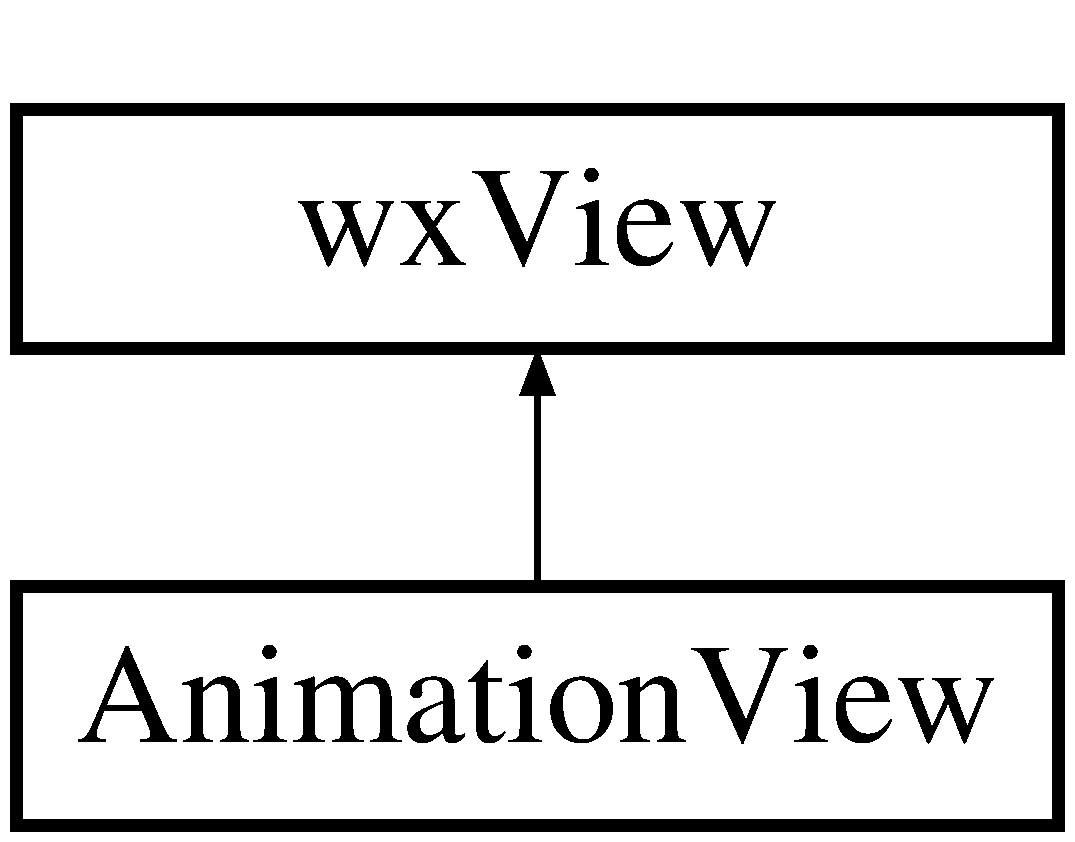
\includegraphics[height=2.000000cm]{a00015}
\end{center}
\end{figure}
\subsection*{Public Member Functions}
\begin{DoxyCompactItemize}
\item 
\hyperlink{a00015_af2c298ae67cb2c186e8737179cdba3ad}{Animation\-View} ()
\item 
\hyperlink{a00015_a323847e06af951f0cc47365477afdcf5}{$\sim$\-Animation\-View} ()
\item 
virtual void \hyperlink{a00015_a39f3d07af74a26b75ed4912b7198b1bc}{On\-Draw} (wx\-D\-C $\ast$dc)
\item 
virtual void \hyperlink{a00015_a3dc02247d57367b18dd9dcda40ad8626}{On\-Update} (wx\-View $\ast$sender, wx\-Object $\ast$hint=(wx\-Object $\ast$) N\-U\-L\-L)
\item 
void \hyperlink{a00015_ab929b54b00e41f0458e909335dbca77d}{Refresh\-Frame} ()
\item 
void \hyperlink{a00015_a3c3c70561baa29e3af60a941efd2dd76}{Set\-Collision\-Type} (\hyperlink{a00196_acf6b899fff4fd35a31a3e8884229f118}{Collision\-Warning} col)
\item 
\hyperlink{a00196_acf6b899fff4fd35a31a3e8884229f118}{Collision\-Warning} \hyperlink{a00015_a3614fac0de8823e0f22cdce02b4de27e}{Get\-Collision\-Type} () const 
\item 
void \hyperlink{a00015_ab05ce897b45b980ef1f0549267954917}{Select\-Collisions} ()
\item 
void \hyperlink{a00015_a1112f9aee2dacc91e64dbe6a63b1c5d5}{Generate} ()
\item 
bool \hyperlink{a00015_ac41a66743a4ba425ff8e7789fb168f11}{Prev\-Beat} ()
\item 
bool \hyperlink{a00015_afced9668cf5a51a0019d6775224946da}{Next\-Beat} ()
\item 
void \hyperlink{a00015_a4422666f5d79b66a31db7ff4fb2749e7}{Goto\-Beat} (unsigned i)
\item 
bool \hyperlink{a00015_a2988eb7b09958a1735fbb8383f8cd959}{Prev\-Sheet} ()
\item 
bool \hyperlink{a00015_ad808539513d97506698893ab06f6eef4}{Next\-Sheet} ()
\item 
void \hyperlink{a00015_a75cdecb5f4c40893697fd3d309eae50e}{Goto\-Sheet} (unsigned i)
\item 
void \hyperlink{a00015_a674e7715633f7e794b738ba0e2f64189}{Set\-Selection} (const \hyperlink{a00214_aaec86d4bb87e1e6f0b60e6e551c5e570}{Selection\-List} \&sl)
\item 
int \hyperlink{a00015_aaf26cfb08a4e889581e4ac3f247c3f4f}{Get\-Number\-Sheets} () const 
\item 
int \hyperlink{a00015_a11dea16d04465f72ab1ffa98f4431bd1}{Get\-Current\-Sheet} () const 
\item 
int \hyperlink{a00015_aa9db8beb597d821c9988a9866406c09f}{Get\-Number\-Beats} () const 
\item 
int \hyperlink{a00015_aca12f7783c48af2533482b26d3472b23}{Get\-Current\-Beat} () const 
\item 
wx\-String \hyperlink{a00015_ae5641c2fa7dfbef1ba386bebbeb54a63}{Get\-Status\-Text} () const 
\item 
const \hyperlink{a00029}{C\-C\-\_\-coord} \& \hyperlink{a00015_a4ee016ca6b0925947a8ef86494b47071}{Get\-Show\-Size} () const 
\item 
void \hyperlink{a00015_a1d34cc6101fa85b2ac017600068cc598}{Unselect\-Marchers} ()
\item 
void \hyperlink{a00015_a7b967748023fa51cbacadb320569d998}{Select\-Marchers\-In\-Box} (long mouse\-X\-Start, long mouse\-Y\-Start, long mouse\-X\-End, long mouse\-Y\-End, bool alt\-Down)
\item 
void \hyperlink{a00015_aa93a3db65a7e779d200e89b4a9f91b51}{Toggle\-Timer} ()
\item 
bool \hyperlink{a00015_a574513cf3b5edc1b190864e0c038f328}{On\-Beat} () const 
\item 
\hyperlink{a00027}{C\-C\-\_\-continuity} \hyperlink{a00015_aad7ff439a3d263762b7f6d529bc6cd75}{Get\-Continuity\-On\-Sheet} (unsigned which\-Sheet, \hyperlink{a00216_a68cd84e0300be6f9ff4474682762c9ee}{S\-Y\-M\-B\-O\-L\-\_\-\-T\-Y\-P\-E} which\-Symbol) const 
\item 
const \hyperlink{a00140}{Show\-Mode} \& \hyperlink{a00015_aaf39bba807352809c664721653ea5172}{Get\-Show\-Mode} () const 
\item 
const \hyperlink{a00020}{Cal\-Chart\-Doc} $\ast$ \hyperlink{a00015_aadc2f1190af3d96a1238150a82266bcd}{Get\-Show} () const 
\item 
\hyperlink{a00020}{Cal\-Chart\-Doc} $\ast$ \hyperlink{a00015_a7764c4557b1cc1934b43046f18d51077}{Get\-Show} ()
\item 
boost\-::shared\-\_\-ptr$<$ \hyperlink{a00010}{Animation} $>$ \hyperlink{a00015_aff90f8db8a467972616723eced1a7e89}{Get\-Animation} ()
\end{DoxyCompactItemize}
\subsection*{Private Member Functions}
\begin{DoxyCompactItemize}
\item 
void \hyperlink{a00015_aa460b7eea0b7b1419b35c82dfea8ead5}{On\-Notify\-Status} (const wx\-String \&status)
\item 
bool \hyperlink{a00015_a66ae9999855ae5635ae3b57cfef2fa1f}{On\-Notify\-Error\-List} (const std\-::vector$<$ \hyperlink{a00098}{Error\-Marker} $>$ \&error\-\_\-markers, unsigned sheetnum, const wx\-String \&message)
\item 
const \hyperlink{a00012}{Animation\-Frame} $\ast$ \hyperlink{a00015_a38d7eab0f899609fdc3855c82a50742f}{Get\-Animation\-Frame} () const 
\item 
\hyperlink{a00012}{Animation\-Frame} $\ast$ \hyperlink{a00015_a881c3da184fff75ad5736bccc35cee02}{Get\-Animation\-Frame} ()
\end{DoxyCompactItemize}
\subsection*{Private Attributes}
\begin{DoxyCompactItemize}
\item 
bool \hyperlink{a00015_a99b4e9fd56411a15e3b2d0834f7ee82c}{m\-Error\-Occurred}
\item 
boost\-::shared\-\_\-ptr$<$ \hyperlink{a00010}{Animation} $>$ \hyperlink{a00015_a8b7370c70c1834443cc7b834b9d964fc}{m\-Animation}
\item 
\hyperlink{a00196_acf6b899fff4fd35a31a3e8884229f118}{Collision\-Warning} \hyperlink{a00015_af1157a855b84821ec8c1ab1843f4b655}{m\-Collision\-Warning\-Type}
\end{DoxyCompactItemize}


\subsection{Constructor \& Destructor Documentation}
\hypertarget{a00015_af2c298ae67cb2c186e8737179cdba3ad}{\index{Animation\-View@{Animation\-View}!Animation\-View@{Animation\-View}}
\index{Animation\-View@{Animation\-View}!AnimationView@{Animation\-View}}
\subsubsection[{Animation\-View}]{\setlength{\rightskip}{0pt plus 5cm}Animation\-View\-::\-Animation\-View (
\begin{DoxyParamCaption}
{}
\end{DoxyParamCaption}
)}}\label{a00015_af2c298ae67cb2c186e8737179cdba3ad}
\hypertarget{a00015_a323847e06af951f0cc47365477afdcf5}{\index{Animation\-View@{Animation\-View}!$\sim$\-Animation\-View@{$\sim$\-Animation\-View}}
\index{$\sim$\-Animation\-View@{$\sim$\-Animation\-View}!AnimationView@{Animation\-View}}
\subsubsection[{$\sim$\-Animation\-View}]{\setlength{\rightskip}{0pt plus 5cm}Animation\-View\-::$\sim$\-Animation\-View (
\begin{DoxyParamCaption}
{}
\end{DoxyParamCaption}
)}}\label{a00015_a323847e06af951f0cc47365477afdcf5}


\subsection{Member Function Documentation}
\hypertarget{a00015_a1112f9aee2dacc91e64dbe6a63b1c5d5}{\index{Animation\-View@{Animation\-View}!Generate@{Generate}}
\index{Generate@{Generate}!AnimationView@{Animation\-View}}
\subsubsection[{Generate}]{\setlength{\rightskip}{0pt plus 5cm}void Animation\-View\-::\-Generate (
\begin{DoxyParamCaption}
{}
\end{DoxyParamCaption}
)}}\label{a00015_a1112f9aee2dacc91e64dbe6a63b1c5d5}
\hypertarget{a00015_aff90f8db8a467972616723eced1a7e89}{\index{Animation\-View@{Animation\-View}!Get\-Animation@{Get\-Animation}}
\index{Get\-Animation@{Get\-Animation}!AnimationView@{Animation\-View}}
\subsubsection[{Get\-Animation}]{\setlength{\rightskip}{0pt plus 5cm}boost\-::shared\-\_\-ptr$<$ {\bf Animation} $>$ Animation\-View\-::\-Get\-Animation (
\begin{DoxyParamCaption}
{}
\end{DoxyParamCaption}
)}}\label{a00015_aff90f8db8a467972616723eced1a7e89}
\hypertarget{a00015_a38d7eab0f899609fdc3855c82a50742f}{\index{Animation\-View@{Animation\-View}!Get\-Animation\-Frame@{Get\-Animation\-Frame}}
\index{Get\-Animation\-Frame@{Get\-Animation\-Frame}!AnimationView@{Animation\-View}}
\subsubsection[{Get\-Animation\-Frame}]{\setlength{\rightskip}{0pt plus 5cm}const {\bf Animation\-Frame} $\ast$ Animation\-View\-::\-Get\-Animation\-Frame (
\begin{DoxyParamCaption}
{}
\end{DoxyParamCaption}
) const\hspace{0.3cm}{\ttfamily [private]}}}\label{a00015_a38d7eab0f899609fdc3855c82a50742f}
\hypertarget{a00015_a881c3da184fff75ad5736bccc35cee02}{\index{Animation\-View@{Animation\-View}!Get\-Animation\-Frame@{Get\-Animation\-Frame}}
\index{Get\-Animation\-Frame@{Get\-Animation\-Frame}!AnimationView@{Animation\-View}}
\subsubsection[{Get\-Animation\-Frame}]{\setlength{\rightskip}{0pt plus 5cm}{\bf Animation\-Frame} $\ast$ Animation\-View\-::\-Get\-Animation\-Frame (
\begin{DoxyParamCaption}
{}
\end{DoxyParamCaption}
)\hspace{0.3cm}{\ttfamily [private]}}}\label{a00015_a881c3da184fff75ad5736bccc35cee02}
\hypertarget{a00015_a3614fac0de8823e0f22cdce02b4de27e}{\index{Animation\-View@{Animation\-View}!Get\-Collision\-Type@{Get\-Collision\-Type}}
\index{Get\-Collision\-Type@{Get\-Collision\-Type}!AnimationView@{Animation\-View}}
\subsubsection[{Get\-Collision\-Type}]{\setlength{\rightskip}{0pt plus 5cm}{\bf Collision\-Warning} Animation\-View\-::\-Get\-Collision\-Type (
\begin{DoxyParamCaption}
{}
\end{DoxyParamCaption}
) const\hspace{0.3cm}{\ttfamily [inline]}}}\label{a00015_a3614fac0de8823e0f22cdce02b4de27e}
\hypertarget{a00015_aad7ff439a3d263762b7f6d529bc6cd75}{\index{Animation\-View@{Animation\-View}!Get\-Continuity\-On\-Sheet@{Get\-Continuity\-On\-Sheet}}
\index{Get\-Continuity\-On\-Sheet@{Get\-Continuity\-On\-Sheet}!AnimationView@{Animation\-View}}
\subsubsection[{Get\-Continuity\-On\-Sheet}]{\setlength{\rightskip}{0pt plus 5cm}{\bf C\-C\-\_\-continuity} Animation\-View\-::\-Get\-Continuity\-On\-Sheet (
\begin{DoxyParamCaption}
\item[{unsigned}]{which\-Sheet, }
\item[{{\bf S\-Y\-M\-B\-O\-L\-\_\-\-T\-Y\-P\-E}}]{which\-Symbol}
\end{DoxyParamCaption}
) const}}\label{a00015_aad7ff439a3d263762b7f6d529bc6cd75}
\hypertarget{a00015_aca12f7783c48af2533482b26d3472b23}{\index{Animation\-View@{Animation\-View}!Get\-Current\-Beat@{Get\-Current\-Beat}}
\index{Get\-Current\-Beat@{Get\-Current\-Beat}!AnimationView@{Animation\-View}}
\subsubsection[{Get\-Current\-Beat}]{\setlength{\rightskip}{0pt plus 5cm}int Animation\-View\-::\-Get\-Current\-Beat (
\begin{DoxyParamCaption}
{}
\end{DoxyParamCaption}
) const}}\label{a00015_aca12f7783c48af2533482b26d3472b23}
\hypertarget{a00015_a11dea16d04465f72ab1ffa98f4431bd1}{\index{Animation\-View@{Animation\-View}!Get\-Current\-Sheet@{Get\-Current\-Sheet}}
\index{Get\-Current\-Sheet@{Get\-Current\-Sheet}!AnimationView@{Animation\-View}}
\subsubsection[{Get\-Current\-Sheet}]{\setlength{\rightskip}{0pt plus 5cm}int Animation\-View\-::\-Get\-Current\-Sheet (
\begin{DoxyParamCaption}
{}
\end{DoxyParamCaption}
) const}}\label{a00015_a11dea16d04465f72ab1ffa98f4431bd1}
\hypertarget{a00015_aa9db8beb597d821c9988a9866406c09f}{\index{Animation\-View@{Animation\-View}!Get\-Number\-Beats@{Get\-Number\-Beats}}
\index{Get\-Number\-Beats@{Get\-Number\-Beats}!AnimationView@{Animation\-View}}
\subsubsection[{Get\-Number\-Beats}]{\setlength{\rightskip}{0pt plus 5cm}int Animation\-View\-::\-Get\-Number\-Beats (
\begin{DoxyParamCaption}
{}
\end{DoxyParamCaption}
) const}}\label{a00015_aa9db8beb597d821c9988a9866406c09f}
\hypertarget{a00015_aaf26cfb08a4e889581e4ac3f247c3f4f}{\index{Animation\-View@{Animation\-View}!Get\-Number\-Sheets@{Get\-Number\-Sheets}}
\index{Get\-Number\-Sheets@{Get\-Number\-Sheets}!AnimationView@{Animation\-View}}
\subsubsection[{Get\-Number\-Sheets}]{\setlength{\rightskip}{0pt plus 5cm}int Animation\-View\-::\-Get\-Number\-Sheets (
\begin{DoxyParamCaption}
{}
\end{DoxyParamCaption}
) const}}\label{a00015_aaf26cfb08a4e889581e4ac3f247c3f4f}
\hypertarget{a00015_aadc2f1190af3d96a1238150a82266bcd}{\index{Animation\-View@{Animation\-View}!Get\-Show@{Get\-Show}}
\index{Get\-Show@{Get\-Show}!AnimationView@{Animation\-View}}
\subsubsection[{Get\-Show}]{\setlength{\rightskip}{0pt plus 5cm}const {\bf Cal\-Chart\-Doc} $\ast$ Animation\-View\-::\-Get\-Show (
\begin{DoxyParamCaption}
{}
\end{DoxyParamCaption}
) const}}\label{a00015_aadc2f1190af3d96a1238150a82266bcd}
\hypertarget{a00015_a7764c4557b1cc1934b43046f18d51077}{\index{Animation\-View@{Animation\-View}!Get\-Show@{Get\-Show}}
\index{Get\-Show@{Get\-Show}!AnimationView@{Animation\-View}}
\subsubsection[{Get\-Show}]{\setlength{\rightskip}{0pt plus 5cm}{\bf Cal\-Chart\-Doc} $\ast$ Animation\-View\-::\-Get\-Show (
\begin{DoxyParamCaption}
{}
\end{DoxyParamCaption}
)}}\label{a00015_a7764c4557b1cc1934b43046f18d51077}
\hypertarget{a00015_aaf39bba807352809c664721653ea5172}{\index{Animation\-View@{Animation\-View}!Get\-Show\-Mode@{Get\-Show\-Mode}}
\index{Get\-Show\-Mode@{Get\-Show\-Mode}!AnimationView@{Animation\-View}}
\subsubsection[{Get\-Show\-Mode}]{\setlength{\rightskip}{0pt plus 5cm}const {\bf Show\-Mode}\& Animation\-View\-::\-Get\-Show\-Mode (
\begin{DoxyParamCaption}
{}
\end{DoxyParamCaption}
) const}}\label{a00015_aaf39bba807352809c664721653ea5172}
\hypertarget{a00015_a4ee016ca6b0925947a8ef86494b47071}{\index{Animation\-View@{Animation\-View}!Get\-Show\-Size@{Get\-Show\-Size}}
\index{Get\-Show\-Size@{Get\-Show\-Size}!AnimationView@{Animation\-View}}
\subsubsection[{Get\-Show\-Size}]{\setlength{\rightskip}{0pt plus 5cm}const {\bf C\-C\-\_\-coord} \& Animation\-View\-::\-Get\-Show\-Size (
\begin{DoxyParamCaption}
{}
\end{DoxyParamCaption}
) const}}\label{a00015_a4ee016ca6b0925947a8ef86494b47071}
\hypertarget{a00015_ae5641c2fa7dfbef1ba386bebbeb54a63}{\index{Animation\-View@{Animation\-View}!Get\-Status\-Text@{Get\-Status\-Text}}
\index{Get\-Status\-Text@{Get\-Status\-Text}!AnimationView@{Animation\-View}}
\subsubsection[{Get\-Status\-Text}]{\setlength{\rightskip}{0pt plus 5cm}wx\-String Animation\-View\-::\-Get\-Status\-Text (
\begin{DoxyParamCaption}
{}
\end{DoxyParamCaption}
) const}}\label{a00015_ae5641c2fa7dfbef1ba386bebbeb54a63}
\hypertarget{a00015_a4422666f5d79b66a31db7ff4fb2749e7}{\index{Animation\-View@{Animation\-View}!Goto\-Beat@{Goto\-Beat}}
\index{Goto\-Beat@{Goto\-Beat}!AnimationView@{Animation\-View}}
\subsubsection[{Goto\-Beat}]{\setlength{\rightskip}{0pt plus 5cm}void Animation\-View\-::\-Goto\-Beat (
\begin{DoxyParamCaption}
\item[{unsigned}]{i}
\end{DoxyParamCaption}
)}}\label{a00015_a4422666f5d79b66a31db7ff4fb2749e7}
\hypertarget{a00015_a75cdecb5f4c40893697fd3d309eae50e}{\index{Animation\-View@{Animation\-View}!Goto\-Sheet@{Goto\-Sheet}}
\index{Goto\-Sheet@{Goto\-Sheet}!AnimationView@{Animation\-View}}
\subsubsection[{Goto\-Sheet}]{\setlength{\rightskip}{0pt plus 5cm}void Animation\-View\-::\-Goto\-Sheet (
\begin{DoxyParamCaption}
\item[{unsigned}]{i}
\end{DoxyParamCaption}
)}}\label{a00015_a75cdecb5f4c40893697fd3d309eae50e}
\hypertarget{a00015_afced9668cf5a51a0019d6775224946da}{\index{Animation\-View@{Animation\-View}!Next\-Beat@{Next\-Beat}}
\index{Next\-Beat@{Next\-Beat}!AnimationView@{Animation\-View}}
\subsubsection[{Next\-Beat}]{\setlength{\rightskip}{0pt plus 5cm}bool Animation\-View\-::\-Next\-Beat (
\begin{DoxyParamCaption}
{}
\end{DoxyParamCaption}
)}}\label{a00015_afced9668cf5a51a0019d6775224946da}
\hypertarget{a00015_ad808539513d97506698893ab06f6eef4}{\index{Animation\-View@{Animation\-View}!Next\-Sheet@{Next\-Sheet}}
\index{Next\-Sheet@{Next\-Sheet}!AnimationView@{Animation\-View}}
\subsubsection[{Next\-Sheet}]{\setlength{\rightskip}{0pt plus 5cm}bool Animation\-View\-::\-Next\-Sheet (
\begin{DoxyParamCaption}
{}
\end{DoxyParamCaption}
)}}\label{a00015_ad808539513d97506698893ab06f6eef4}
\hypertarget{a00015_a574513cf3b5edc1b190864e0c038f328}{\index{Animation\-View@{Animation\-View}!On\-Beat@{On\-Beat}}
\index{On\-Beat@{On\-Beat}!AnimationView@{Animation\-View}}
\subsubsection[{On\-Beat}]{\setlength{\rightskip}{0pt plus 5cm}bool Animation\-View\-::\-On\-Beat (
\begin{DoxyParamCaption}
{}
\end{DoxyParamCaption}
) const}}\label{a00015_a574513cf3b5edc1b190864e0c038f328}
\hypertarget{a00015_a39f3d07af74a26b75ed4912b7198b1bc}{\index{Animation\-View@{Animation\-View}!On\-Draw@{On\-Draw}}
\index{On\-Draw@{On\-Draw}!AnimationView@{Animation\-View}}
\subsubsection[{On\-Draw}]{\setlength{\rightskip}{0pt plus 5cm}void Animation\-View\-::\-On\-Draw (
\begin{DoxyParamCaption}
\item[{wx\-D\-C $\ast$}]{dc}
\end{DoxyParamCaption}
)\hspace{0.3cm}{\ttfamily [virtual]}}}\label{a00015_a39f3d07af74a26b75ed4912b7198b1bc}
\hypertarget{a00015_a66ae9999855ae5635ae3b57cfef2fa1f}{\index{Animation\-View@{Animation\-View}!On\-Notify\-Error\-List@{On\-Notify\-Error\-List}}
\index{On\-Notify\-Error\-List@{On\-Notify\-Error\-List}!AnimationView@{Animation\-View}}
\subsubsection[{On\-Notify\-Error\-List}]{\setlength{\rightskip}{0pt plus 5cm}bool Animation\-View\-::\-On\-Notify\-Error\-List (
\begin{DoxyParamCaption}
\item[{const std\-::vector$<$ {\bf Error\-Marker} $>$ \&}]{error\-\_\-markers, }
\item[{unsigned}]{sheetnum, }
\item[{const wx\-String \&}]{message}
\end{DoxyParamCaption}
)\hspace{0.3cm}{\ttfamily [private]}}}\label{a00015_a66ae9999855ae5635ae3b57cfef2fa1f}
\hypertarget{a00015_aa460b7eea0b7b1419b35c82dfea8ead5}{\index{Animation\-View@{Animation\-View}!On\-Notify\-Status@{On\-Notify\-Status}}
\index{On\-Notify\-Status@{On\-Notify\-Status}!AnimationView@{Animation\-View}}
\subsubsection[{On\-Notify\-Status}]{\setlength{\rightskip}{0pt plus 5cm}void Animation\-View\-::\-On\-Notify\-Status (
\begin{DoxyParamCaption}
\item[{const wx\-String \&}]{status}
\end{DoxyParamCaption}
)\hspace{0.3cm}{\ttfamily [private]}}}\label{a00015_aa460b7eea0b7b1419b35c82dfea8ead5}
\hypertarget{a00015_a3dc02247d57367b18dd9dcda40ad8626}{\index{Animation\-View@{Animation\-View}!On\-Update@{On\-Update}}
\index{On\-Update@{On\-Update}!AnimationView@{Animation\-View}}
\subsubsection[{On\-Update}]{\setlength{\rightskip}{0pt plus 5cm}void Animation\-View\-::\-On\-Update (
\begin{DoxyParamCaption}
\item[{wx\-View $\ast$}]{sender, }
\item[{wx\-Object $\ast$}]{hint = {\ttfamily (wxObject~$\ast$)~NULL}}
\end{DoxyParamCaption}
)\hspace{0.3cm}{\ttfamily [virtual]}}}\label{a00015_a3dc02247d57367b18dd9dcda40ad8626}
\hypertarget{a00015_ac41a66743a4ba425ff8e7789fb168f11}{\index{Animation\-View@{Animation\-View}!Prev\-Beat@{Prev\-Beat}}
\index{Prev\-Beat@{Prev\-Beat}!AnimationView@{Animation\-View}}
\subsubsection[{Prev\-Beat}]{\setlength{\rightskip}{0pt plus 5cm}bool Animation\-View\-::\-Prev\-Beat (
\begin{DoxyParamCaption}
{}
\end{DoxyParamCaption}
)}}\label{a00015_ac41a66743a4ba425ff8e7789fb168f11}
\hypertarget{a00015_a2988eb7b09958a1735fbb8383f8cd959}{\index{Animation\-View@{Animation\-View}!Prev\-Sheet@{Prev\-Sheet}}
\index{Prev\-Sheet@{Prev\-Sheet}!AnimationView@{Animation\-View}}
\subsubsection[{Prev\-Sheet}]{\setlength{\rightskip}{0pt plus 5cm}bool Animation\-View\-::\-Prev\-Sheet (
\begin{DoxyParamCaption}
{}
\end{DoxyParamCaption}
)}}\label{a00015_a2988eb7b09958a1735fbb8383f8cd959}
\hypertarget{a00015_ab929b54b00e41f0458e909335dbca77d}{\index{Animation\-View@{Animation\-View}!Refresh\-Frame@{Refresh\-Frame}}
\index{Refresh\-Frame@{Refresh\-Frame}!AnimationView@{Animation\-View}}
\subsubsection[{Refresh\-Frame}]{\setlength{\rightskip}{0pt plus 5cm}void Animation\-View\-::\-Refresh\-Frame (
\begin{DoxyParamCaption}
{}
\end{DoxyParamCaption}
)}}\label{a00015_ab929b54b00e41f0458e909335dbca77d}
\hypertarget{a00015_ab05ce897b45b980ef1f0549267954917}{\index{Animation\-View@{Animation\-View}!Select\-Collisions@{Select\-Collisions}}
\index{Select\-Collisions@{Select\-Collisions}!AnimationView@{Animation\-View}}
\subsubsection[{Select\-Collisions}]{\setlength{\rightskip}{0pt plus 5cm}void Animation\-View\-::\-Select\-Collisions (
\begin{DoxyParamCaption}
{}
\end{DoxyParamCaption}
)}}\label{a00015_ab05ce897b45b980ef1f0549267954917}
\hypertarget{a00015_a7b967748023fa51cbacadb320569d998}{\index{Animation\-View@{Animation\-View}!Select\-Marchers\-In\-Box@{Select\-Marchers\-In\-Box}}
\index{Select\-Marchers\-In\-Box@{Select\-Marchers\-In\-Box}!AnimationView@{Animation\-View}}
\subsubsection[{Select\-Marchers\-In\-Box}]{\setlength{\rightskip}{0pt plus 5cm}void Animation\-View\-::\-Select\-Marchers\-In\-Box (
\begin{DoxyParamCaption}
\item[{long}]{mouse\-X\-Start, }
\item[{long}]{mouse\-Y\-Start, }
\item[{long}]{mouse\-X\-End, }
\item[{long}]{mouse\-Y\-End, }
\item[{bool}]{alt\-Down}
\end{DoxyParamCaption}
)}}\label{a00015_a7b967748023fa51cbacadb320569d998}
\hypertarget{a00015_a3c3c70561baa29e3af60a941efd2dd76}{\index{Animation\-View@{Animation\-View}!Set\-Collision\-Type@{Set\-Collision\-Type}}
\index{Set\-Collision\-Type@{Set\-Collision\-Type}!AnimationView@{Animation\-View}}
\subsubsection[{Set\-Collision\-Type}]{\setlength{\rightskip}{0pt plus 5cm}void Animation\-View\-::\-Set\-Collision\-Type (
\begin{DoxyParamCaption}
\item[{{\bf Collision\-Warning}}]{col}
\end{DoxyParamCaption}
)}}\label{a00015_a3c3c70561baa29e3af60a941efd2dd76}
\hypertarget{a00015_a674e7715633f7e794b738ba0e2f64189}{\index{Animation\-View@{Animation\-View}!Set\-Selection@{Set\-Selection}}
\index{Set\-Selection@{Set\-Selection}!AnimationView@{Animation\-View}}
\subsubsection[{Set\-Selection}]{\setlength{\rightskip}{0pt plus 5cm}void Animation\-View\-::\-Set\-Selection (
\begin{DoxyParamCaption}
\item[{const {\bf Selection\-List} \&}]{sl}
\end{DoxyParamCaption}
)}}\label{a00015_a674e7715633f7e794b738ba0e2f64189}
\hypertarget{a00015_aa93a3db65a7e779d200e89b4a9f91b51}{\index{Animation\-View@{Animation\-View}!Toggle\-Timer@{Toggle\-Timer}}
\index{Toggle\-Timer@{Toggle\-Timer}!AnimationView@{Animation\-View}}
\subsubsection[{Toggle\-Timer}]{\setlength{\rightskip}{0pt plus 5cm}void Animation\-View\-::\-Toggle\-Timer (
\begin{DoxyParamCaption}
{}
\end{DoxyParamCaption}
)}}\label{a00015_aa93a3db65a7e779d200e89b4a9f91b51}
\hypertarget{a00015_a1d34cc6101fa85b2ac017600068cc598}{\index{Animation\-View@{Animation\-View}!Unselect\-Marchers@{Unselect\-Marchers}}
\index{Unselect\-Marchers@{Unselect\-Marchers}!AnimationView@{Animation\-View}}
\subsubsection[{Unselect\-Marchers}]{\setlength{\rightskip}{0pt plus 5cm}void Animation\-View\-::\-Unselect\-Marchers (
\begin{DoxyParamCaption}
{}
\end{DoxyParamCaption}
)}}\label{a00015_a1d34cc6101fa85b2ac017600068cc598}


\subsection{Member Data Documentation}
\hypertarget{a00015_a8b7370c70c1834443cc7b834b9d964fc}{\index{Animation\-View@{Animation\-View}!m\-Animation@{m\-Animation}}
\index{m\-Animation@{m\-Animation}!AnimationView@{Animation\-View}}
\subsubsection[{m\-Animation}]{\setlength{\rightskip}{0pt plus 5cm}boost\-::shared\-\_\-ptr$<${\bf Animation}$>$ Animation\-View\-::m\-Animation\hspace{0.3cm}{\ttfamily [private]}}}\label{a00015_a8b7370c70c1834443cc7b834b9d964fc}
\hypertarget{a00015_af1157a855b84821ec8c1ab1843f4b655}{\index{Animation\-View@{Animation\-View}!m\-Collision\-Warning\-Type@{m\-Collision\-Warning\-Type}}
\index{m\-Collision\-Warning\-Type@{m\-Collision\-Warning\-Type}!AnimationView@{Animation\-View}}
\subsubsection[{m\-Collision\-Warning\-Type}]{\setlength{\rightskip}{0pt plus 5cm}{\bf Collision\-Warning} Animation\-View\-::m\-Collision\-Warning\-Type\hspace{0.3cm}{\ttfamily [private]}}}\label{a00015_af1157a855b84821ec8c1ab1843f4b655}
\hypertarget{a00015_a99b4e9fd56411a15e3b2d0834f7ee82c}{\index{Animation\-View@{Animation\-View}!m\-Error\-Occurred@{m\-Error\-Occurred}}
\index{m\-Error\-Occurred@{m\-Error\-Occurred}!AnimationView@{Animation\-View}}
\subsubsection[{m\-Error\-Occurred}]{\setlength{\rightskip}{0pt plus 5cm}bool Animation\-View\-::m\-Error\-Occurred\hspace{0.3cm}{\ttfamily [private]}}}\label{a00015_a99b4e9fd56411a15e3b2d0834f7ee82c}


The documentation for this class was generated from the following files\-:\begin{DoxyCompactItemize}
\item 
src/\hyperlink{a00173}{animation\-\_\-view.\-h}\item 
src/\hyperlink{a00172}{animation\-\_\-view.\-cpp}\end{DoxyCompactItemize}

\hypertarget{a00016}{\section{Cal\-Chart\-Doc\-:\-:Auto\-Save\-Timer Class Reference}
\label{a00016}\index{Cal\-Chart\-Doc\-::\-Auto\-Save\-Timer@{Cal\-Chart\-Doc\-::\-Auto\-Save\-Timer}}
}
Inheritance diagram for Cal\-Chart\-Doc\-:\-:Auto\-Save\-Timer\-:\begin{figure}[H]
\begin{center}
\leavevmode
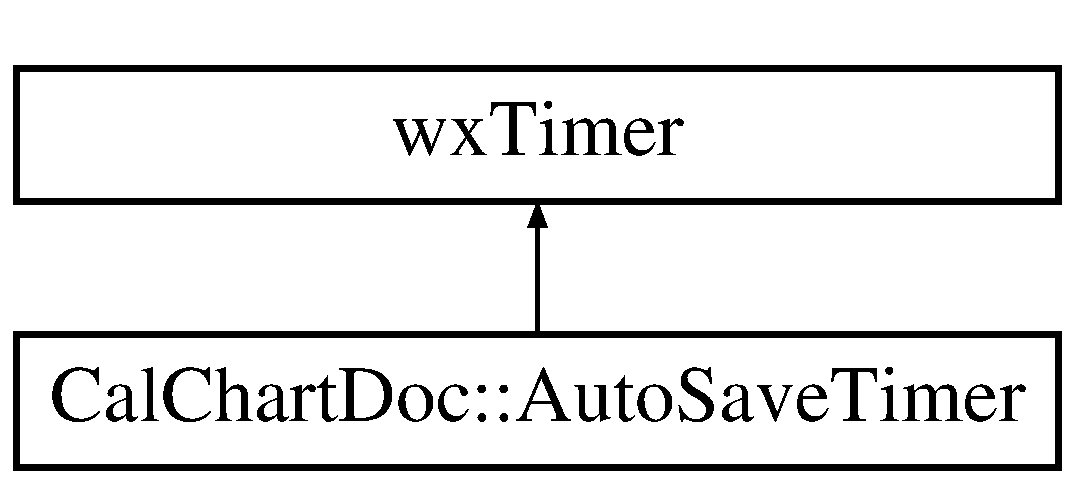
\includegraphics[height=2.000000cm]{a00016}
\end{center}
\end{figure}
\subsection*{Public Member Functions}
\begin{DoxyCompactItemize}
\item 
\hyperlink{a00016_ab3a4e3558500deff01c63a33317b2518}{Auto\-Save\-Timer} (\hyperlink{a00020}{Cal\-Chart\-Doc} \&show)
\item 
void \hyperlink{a00016_a733c93f1fdaf21d7d3d9b1f6cc683da5}{Notify} ()
\end{DoxyCompactItemize}
\subsection*{Private Attributes}
\begin{DoxyCompactItemize}
\item 
\hyperlink{a00020}{Cal\-Chart\-Doc} \& \hyperlink{a00016_a77bf8094ea3bbd05d67f3ba3b3efac1f}{m\-Show}
\end{DoxyCompactItemize}


\subsection{Constructor \& Destructor Documentation}
\hypertarget{a00016_ab3a4e3558500deff01c63a33317b2518}{\index{Cal\-Chart\-Doc\-::\-Auto\-Save\-Timer@{Cal\-Chart\-Doc\-::\-Auto\-Save\-Timer}!Auto\-Save\-Timer@{Auto\-Save\-Timer}}
\index{Auto\-Save\-Timer@{Auto\-Save\-Timer}!CalChartDoc::AutoSaveTimer@{Cal\-Chart\-Doc\-::\-Auto\-Save\-Timer}}
\subsubsection[{Auto\-Save\-Timer}]{\setlength{\rightskip}{0pt plus 5cm}Cal\-Chart\-Doc\-::\-Auto\-Save\-Timer\-::\-Auto\-Save\-Timer (
\begin{DoxyParamCaption}
\item[{{\bf Cal\-Chart\-Doc} \&}]{show}
\end{DoxyParamCaption}
)\hspace{0.3cm}{\ttfamily [inline]}}}\label{a00016_ab3a4e3558500deff01c63a33317b2518}


\subsection{Member Function Documentation}
\hypertarget{a00016_a733c93f1fdaf21d7d3d9b1f6cc683da5}{\index{Cal\-Chart\-Doc\-::\-Auto\-Save\-Timer@{Cal\-Chart\-Doc\-::\-Auto\-Save\-Timer}!Notify@{Notify}}
\index{Notify@{Notify}!CalChartDoc::AutoSaveTimer@{Cal\-Chart\-Doc\-::\-Auto\-Save\-Timer}}
\subsubsection[{Notify}]{\setlength{\rightskip}{0pt plus 5cm}void Cal\-Chart\-Doc\-::\-Auto\-Save\-Timer\-::\-Notify (
\begin{DoxyParamCaption}
{}
\end{DoxyParamCaption}
)}}\label{a00016_a733c93f1fdaf21d7d3d9b1f6cc683da5}


\subsection{Member Data Documentation}
\hypertarget{a00016_a77bf8094ea3bbd05d67f3ba3b3efac1f}{\index{Cal\-Chart\-Doc\-::\-Auto\-Save\-Timer@{Cal\-Chart\-Doc\-::\-Auto\-Save\-Timer}!m\-Show@{m\-Show}}
\index{m\-Show@{m\-Show}!CalChartDoc::AutoSaveTimer@{Cal\-Chart\-Doc\-::\-Auto\-Save\-Timer}}
\subsubsection[{m\-Show}]{\setlength{\rightskip}{0pt plus 5cm}{\bf Cal\-Chart\-Doc}\& Cal\-Chart\-Doc\-::\-Auto\-Save\-Timer\-::m\-Show\hspace{0.3cm}{\ttfamily [private]}}}\label{a00016_a77bf8094ea3bbd05d67f3ba3b3efac1f}


The documentation for this class was generated from the following files\-:\begin{DoxyCompactItemize}
\item 
src/\hyperlink{a00181}{calchartdoc.\-h}\item 
src/\hyperlink{a00180}{calchartdoc.\-cpp}\end{DoxyCompactItemize}

\hypertarget{a00017}{\section{Background\-Image Class Reference}
\label{a00017}\index{Background\-Image@{Background\-Image}}
}


{\ttfamily \#include $<$background\-\_\-image.\-h$>$}

\subsection*{Classes}
\begin{DoxyCompactItemize}
\item 
class \hyperlink{a00026}{Calculate\-Scale\-And\-Move}
\end{DoxyCompactItemize}
\subsection*{Public Member Functions}
\begin{DoxyCompactItemize}
\item 
\hyperlink{a00017_a29939f6b581d864b8bca97063890c0ae}{Background\-Image} (const wx\-Image \&image, const wx\-Coord \&x, const wx\-Coord \&y)
\item 
void \hyperlink{a00017_a581572e942b22b6f035738644936f7e8}{On\-Mouse\-Left\-Down} (const wx\-Mouse\-Event \&event, const wx\-D\-C \&dc)
\item 
void \hyperlink{a00017_a1aaca3506e3303df61daaddbaac43017}{On\-Mouse\-Left\-Up} (const wx\-Mouse\-Event \&event, const wx\-D\-C \&dc)
\item 
void \hyperlink{a00017_afc127d8e4bdcd37f6bb62116a32a7ecb}{On\-Mouse\-Move} (const wx\-Mouse\-Event \&event, const wx\-D\-C \&dc)
\item 
void \hyperlink{a00017_a4ab0518bd790d9b00ff1f7e777e2cca2}{On\-Paint} (wx\-D\-C \&dc)
\item 
bool \hyperlink{a00017_a0c4359024d9144013cdc81cbbd9fb2f9}{Doing\-Picture\-Adjustment} ()
\item 
void \hyperlink{a00017_a3c736dc98d1a9f5238fd51e2b0316744}{Do\-Picture\-Adjustment} (bool enable)
\end{DoxyCompactItemize}
\subsection*{Private Types}
\begin{DoxyCompactItemize}
\item 
enum \hyperlink{a00017_a3927289a3b88bbf9320c2dfe3271c1ae}{e\-Background\-Adjust\-Type} \{ \\*
\hyperlink{a00017_a3927289a3b88bbf9320c2dfe3271c1aea72bd60a19a032bf6ee119dadfa2d3d29}{k\-Upper\-Left} = 0, 
\hyperlink{a00017_a3927289a3b88bbf9320c2dfe3271c1aeabffc7e6bb348a607df81178f547d6e56}{k\-Upper}, 
\hyperlink{a00017_a3927289a3b88bbf9320c2dfe3271c1aeadcf35ed4269172ba63c0e4f69c67358e}{k\-Upper\-Right}, 
\hyperlink{a00017_a3927289a3b88bbf9320c2dfe3271c1aea3b504f62c925ffe2a61686791dfd50ce}{k\-Left}, 
\\*
\hyperlink{a00017_a3927289a3b88bbf9320c2dfe3271c1aea7e36cbc14ee765b91ff48bfb919ef803}{k\-Move}, 
\hyperlink{a00017_a3927289a3b88bbf9320c2dfe3271c1aeac38ecb64d242697f4c7f97a8313d3eb3}{k\-Right}, 
\hyperlink{a00017_a3927289a3b88bbf9320c2dfe3271c1aea1abc7f0f5977ff39029443feed7faa00}{k\-Lower\-Left}, 
\hyperlink{a00017_a3927289a3b88bbf9320c2dfe3271c1aea7fe4ae3c7ccff056364ec92208f9f59b}{k\-Lower}, 
\\*
\hyperlink{a00017_a3927289a3b88bbf9320c2dfe3271c1aea85dacb13f2a7ec3cd034f0979e417a92}{k\-Lower\-Right}, 
\hyperlink{a00017_a3927289a3b88bbf9320c2dfe3271c1aea3a3853b41c9d43cf9f5d761ce167c56c}{k\-Last}
 \}
\end{DoxyCompactItemize}
\subsection*{Private Attributes}
\begin{DoxyCompactItemize}
\item 
wx\-Image \hyperlink{a00017_a121b7518d160cb9253ca79d44441ab57}{m\-Image}
\item 
wx\-Bitmap \hyperlink{a00017_aeeb255c7ec155b17ead559e9302808ec}{m\-Bitmap}
\item 
wx\-Coord \hyperlink{a00017_a9a6be1ca346b8c606143580e25217e98}{m\-Bitmap\-X}
\item 
wx\-Coord \hyperlink{a00017_a45f1e5d433635255d53040a31d778b8e}{m\-Bitmap\-Y}
\item 
bool \hyperlink{a00017_a3573c3aaaa7cab651194764a97e6beb1}{m\-Do\-Background\-Pic\-Adjust}
\item 
\hyperlink{a00017_a3927289a3b88bbf9320c2dfe3271c1ae}{e\-Background\-Adjust\-Type} \hyperlink{a00017_a297fe7a109d02b72f877d598f9d72053}{m\-Background\-Adjust\-Type}
\item 
boost\-::shared\-\_\-ptr\\*
$<$ \hyperlink{a00026}{Calculate\-Scale\-And\-Move} $>$ \hyperlink{a00017_a04635fba985907271247cb8bf1b58bfb}{m\-Scale\-And\-Move}
\end{DoxyCompactItemize}
\subsection*{Static Private Attributes}
\begin{DoxyCompactItemize}
\item 
static const long \hyperlink{a00017_a0a6ebc863581593e9be0666a273dd634}{k\-Circle\-Size} = 6
\end{DoxyCompactItemize}


\subsection{Member Enumeration Documentation}
\hypertarget{a00017_a3927289a3b88bbf9320c2dfe3271c1ae}{\index{Background\-Image@{Background\-Image}!e\-Background\-Adjust\-Type@{e\-Background\-Adjust\-Type}}
\index{e\-Background\-Adjust\-Type@{e\-Background\-Adjust\-Type}!BackgroundImage@{Background\-Image}}
\subsubsection[{e\-Background\-Adjust\-Type}]{\setlength{\rightskip}{0pt plus 5cm}enum {\bf Background\-Image\-::e\-Background\-Adjust\-Type}\hspace{0.3cm}{\ttfamily [private]}}}\label{a00017_a3927289a3b88bbf9320c2dfe3271c1ae}
\begin{Desc}
\item[Enumerator]\par
\begin{description}
\index{k\-Upper\-Left@{k\-Upper\-Left}!Background\-Image@{Background\-Image}}\index{Background\-Image@{Background\-Image}!k\-Upper\-Left@{k\-Upper\-Left}}\item[{\em 
\hypertarget{a00017_a3927289a3b88bbf9320c2dfe3271c1aea72bd60a19a032bf6ee119dadfa2d3d29}{k\-Upper\-Left}\label{a00017_a3927289a3b88bbf9320c2dfe3271c1aea72bd60a19a032bf6ee119dadfa2d3d29}
}]\index{k\-Upper@{k\-Upper}!Background\-Image@{Background\-Image}}\index{Background\-Image@{Background\-Image}!k\-Upper@{k\-Upper}}\item[{\em 
\hypertarget{a00017_a3927289a3b88bbf9320c2dfe3271c1aeabffc7e6bb348a607df81178f547d6e56}{k\-Upper}\label{a00017_a3927289a3b88bbf9320c2dfe3271c1aeabffc7e6bb348a607df81178f547d6e56}
}]\index{k\-Upper\-Right@{k\-Upper\-Right}!Background\-Image@{Background\-Image}}\index{Background\-Image@{Background\-Image}!k\-Upper\-Right@{k\-Upper\-Right}}\item[{\em 
\hypertarget{a00017_a3927289a3b88bbf9320c2dfe3271c1aeadcf35ed4269172ba63c0e4f69c67358e}{k\-Upper\-Right}\label{a00017_a3927289a3b88bbf9320c2dfe3271c1aeadcf35ed4269172ba63c0e4f69c67358e}
}]\index{k\-Left@{k\-Left}!Background\-Image@{Background\-Image}}\index{Background\-Image@{Background\-Image}!k\-Left@{k\-Left}}\item[{\em 
\hypertarget{a00017_a3927289a3b88bbf9320c2dfe3271c1aea3b504f62c925ffe2a61686791dfd50ce}{k\-Left}\label{a00017_a3927289a3b88bbf9320c2dfe3271c1aea3b504f62c925ffe2a61686791dfd50ce}
}]\index{k\-Move@{k\-Move}!Background\-Image@{Background\-Image}}\index{Background\-Image@{Background\-Image}!k\-Move@{k\-Move}}\item[{\em 
\hypertarget{a00017_a3927289a3b88bbf9320c2dfe3271c1aea7e36cbc14ee765b91ff48bfb919ef803}{k\-Move}\label{a00017_a3927289a3b88bbf9320c2dfe3271c1aea7e36cbc14ee765b91ff48bfb919ef803}
}]\index{k\-Right@{k\-Right}!Background\-Image@{Background\-Image}}\index{Background\-Image@{Background\-Image}!k\-Right@{k\-Right}}\item[{\em 
\hypertarget{a00017_a3927289a3b88bbf9320c2dfe3271c1aeac38ecb64d242697f4c7f97a8313d3eb3}{k\-Right}\label{a00017_a3927289a3b88bbf9320c2dfe3271c1aeac38ecb64d242697f4c7f97a8313d3eb3}
}]\index{k\-Lower\-Left@{k\-Lower\-Left}!Background\-Image@{Background\-Image}}\index{Background\-Image@{Background\-Image}!k\-Lower\-Left@{k\-Lower\-Left}}\item[{\em 
\hypertarget{a00017_a3927289a3b88bbf9320c2dfe3271c1aea1abc7f0f5977ff39029443feed7faa00}{k\-Lower\-Left}\label{a00017_a3927289a3b88bbf9320c2dfe3271c1aea1abc7f0f5977ff39029443feed7faa00}
}]\index{k\-Lower@{k\-Lower}!Background\-Image@{Background\-Image}}\index{Background\-Image@{Background\-Image}!k\-Lower@{k\-Lower}}\item[{\em 
\hypertarget{a00017_a3927289a3b88bbf9320c2dfe3271c1aea7fe4ae3c7ccff056364ec92208f9f59b}{k\-Lower}\label{a00017_a3927289a3b88bbf9320c2dfe3271c1aea7fe4ae3c7ccff056364ec92208f9f59b}
}]\index{k\-Lower\-Right@{k\-Lower\-Right}!Background\-Image@{Background\-Image}}\index{Background\-Image@{Background\-Image}!k\-Lower\-Right@{k\-Lower\-Right}}\item[{\em 
\hypertarget{a00017_a3927289a3b88bbf9320c2dfe3271c1aea85dacb13f2a7ec3cd034f0979e417a92}{k\-Lower\-Right}\label{a00017_a3927289a3b88bbf9320c2dfe3271c1aea85dacb13f2a7ec3cd034f0979e417a92}
}]\index{k\-Last@{k\-Last}!Background\-Image@{Background\-Image}}\index{Background\-Image@{Background\-Image}!k\-Last@{k\-Last}}\item[{\em 
\hypertarget{a00017_a3927289a3b88bbf9320c2dfe3271c1aea3a3853b41c9d43cf9f5d761ce167c56c}{k\-Last}\label{a00017_a3927289a3b88bbf9320c2dfe3271c1aea3a3853b41c9d43cf9f5d761ce167c56c}
}]\end{description}
\end{Desc}


\subsection{Constructor \& Destructor Documentation}
\hypertarget{a00017_a29939f6b581d864b8bca97063890c0ae}{\index{Background\-Image@{Background\-Image}!Background\-Image@{Background\-Image}}
\index{Background\-Image@{Background\-Image}!BackgroundImage@{Background\-Image}}
\subsubsection[{Background\-Image}]{\setlength{\rightskip}{0pt plus 5cm}Background\-Image\-::\-Background\-Image (
\begin{DoxyParamCaption}
\item[{const wx\-Image \&}]{image, }
\item[{const wx\-Coord \&}]{x, }
\item[{const wx\-Coord \&}]{y}
\end{DoxyParamCaption}
)}}\label{a00017_a29939f6b581d864b8bca97063890c0ae}


\subsection{Member Function Documentation}
\hypertarget{a00017_a0c4359024d9144013cdc81cbbd9fb2f9}{\index{Background\-Image@{Background\-Image}!Doing\-Picture\-Adjustment@{Doing\-Picture\-Adjustment}}
\index{Doing\-Picture\-Adjustment@{Doing\-Picture\-Adjustment}!BackgroundImage@{Background\-Image}}
\subsubsection[{Doing\-Picture\-Adjustment}]{\setlength{\rightskip}{0pt plus 5cm}bool Background\-Image\-::\-Doing\-Picture\-Adjustment (
\begin{DoxyParamCaption}
{}
\end{DoxyParamCaption}
)\hspace{0.3cm}{\ttfamily [inline]}}}\label{a00017_a0c4359024d9144013cdc81cbbd9fb2f9}
\hypertarget{a00017_a3c736dc98d1a9f5238fd51e2b0316744}{\index{Background\-Image@{Background\-Image}!Do\-Picture\-Adjustment@{Do\-Picture\-Adjustment}}
\index{Do\-Picture\-Adjustment@{Do\-Picture\-Adjustment}!BackgroundImage@{Background\-Image}}
\subsubsection[{Do\-Picture\-Adjustment}]{\setlength{\rightskip}{0pt plus 5cm}void Background\-Image\-::\-Do\-Picture\-Adjustment (
\begin{DoxyParamCaption}
\item[{bool}]{enable}
\end{DoxyParamCaption}
)\hspace{0.3cm}{\ttfamily [inline]}}}\label{a00017_a3c736dc98d1a9f5238fd51e2b0316744}
\hypertarget{a00017_a581572e942b22b6f035738644936f7e8}{\index{Background\-Image@{Background\-Image}!On\-Mouse\-Left\-Down@{On\-Mouse\-Left\-Down}}
\index{On\-Mouse\-Left\-Down@{On\-Mouse\-Left\-Down}!BackgroundImage@{Background\-Image}}
\subsubsection[{On\-Mouse\-Left\-Down}]{\setlength{\rightskip}{0pt plus 5cm}void Background\-Image\-::\-On\-Mouse\-Left\-Down (
\begin{DoxyParamCaption}
\item[{const wx\-Mouse\-Event \&}]{event, }
\item[{const wx\-D\-C \&}]{dc}
\end{DoxyParamCaption}
)}}\label{a00017_a581572e942b22b6f035738644936f7e8}
\hypertarget{a00017_a1aaca3506e3303df61daaddbaac43017}{\index{Background\-Image@{Background\-Image}!On\-Mouse\-Left\-Up@{On\-Mouse\-Left\-Up}}
\index{On\-Mouse\-Left\-Up@{On\-Mouse\-Left\-Up}!BackgroundImage@{Background\-Image}}
\subsubsection[{On\-Mouse\-Left\-Up}]{\setlength{\rightskip}{0pt plus 5cm}void Background\-Image\-::\-On\-Mouse\-Left\-Up (
\begin{DoxyParamCaption}
\item[{const wx\-Mouse\-Event \&}]{event, }
\item[{const wx\-D\-C \&}]{dc}
\end{DoxyParamCaption}
)}}\label{a00017_a1aaca3506e3303df61daaddbaac43017}
\hypertarget{a00017_afc127d8e4bdcd37f6bb62116a32a7ecb}{\index{Background\-Image@{Background\-Image}!On\-Mouse\-Move@{On\-Mouse\-Move}}
\index{On\-Mouse\-Move@{On\-Mouse\-Move}!BackgroundImage@{Background\-Image}}
\subsubsection[{On\-Mouse\-Move}]{\setlength{\rightskip}{0pt plus 5cm}void Background\-Image\-::\-On\-Mouse\-Move (
\begin{DoxyParamCaption}
\item[{const wx\-Mouse\-Event \&}]{event, }
\item[{const wx\-D\-C \&}]{dc}
\end{DoxyParamCaption}
)}}\label{a00017_afc127d8e4bdcd37f6bb62116a32a7ecb}
\hypertarget{a00017_a4ab0518bd790d9b00ff1f7e777e2cca2}{\index{Background\-Image@{Background\-Image}!On\-Paint@{On\-Paint}}
\index{On\-Paint@{On\-Paint}!BackgroundImage@{Background\-Image}}
\subsubsection[{On\-Paint}]{\setlength{\rightskip}{0pt plus 5cm}void Background\-Image\-::\-On\-Paint (
\begin{DoxyParamCaption}
\item[{wx\-D\-C \&}]{dc}
\end{DoxyParamCaption}
)}}\label{a00017_a4ab0518bd790d9b00ff1f7e777e2cca2}


\subsection{Member Data Documentation}
\hypertarget{a00017_a0a6ebc863581593e9be0666a273dd634}{\index{Background\-Image@{Background\-Image}!k\-Circle\-Size@{k\-Circle\-Size}}
\index{k\-Circle\-Size@{k\-Circle\-Size}!BackgroundImage@{Background\-Image}}
\subsubsection[{k\-Circle\-Size}]{\setlength{\rightskip}{0pt plus 5cm}const long Background\-Image\-::k\-Circle\-Size = 6\hspace{0.3cm}{\ttfamily [static]}, {\ttfamily [private]}}}\label{a00017_a0a6ebc863581593e9be0666a273dd634}
\hypertarget{a00017_a297fe7a109d02b72f877d598f9d72053}{\index{Background\-Image@{Background\-Image}!m\-Background\-Adjust\-Type@{m\-Background\-Adjust\-Type}}
\index{m\-Background\-Adjust\-Type@{m\-Background\-Adjust\-Type}!BackgroundImage@{Background\-Image}}
\subsubsection[{m\-Background\-Adjust\-Type}]{\setlength{\rightskip}{0pt plus 5cm}{\bf e\-Background\-Adjust\-Type} Background\-Image\-::m\-Background\-Adjust\-Type\hspace{0.3cm}{\ttfamily [private]}}}\label{a00017_a297fe7a109d02b72f877d598f9d72053}
\hypertarget{a00017_aeeb255c7ec155b17ead559e9302808ec}{\index{Background\-Image@{Background\-Image}!m\-Bitmap@{m\-Bitmap}}
\index{m\-Bitmap@{m\-Bitmap}!BackgroundImage@{Background\-Image}}
\subsubsection[{m\-Bitmap}]{\setlength{\rightskip}{0pt plus 5cm}wx\-Bitmap Background\-Image\-::m\-Bitmap\hspace{0.3cm}{\ttfamily [private]}}}\label{a00017_aeeb255c7ec155b17ead559e9302808ec}
\hypertarget{a00017_a9a6be1ca346b8c606143580e25217e98}{\index{Background\-Image@{Background\-Image}!m\-Bitmap\-X@{m\-Bitmap\-X}}
\index{m\-Bitmap\-X@{m\-Bitmap\-X}!BackgroundImage@{Background\-Image}}
\subsubsection[{m\-Bitmap\-X}]{\setlength{\rightskip}{0pt plus 5cm}wx\-Coord Background\-Image\-::m\-Bitmap\-X\hspace{0.3cm}{\ttfamily [private]}}}\label{a00017_a9a6be1ca346b8c606143580e25217e98}
\hypertarget{a00017_a45f1e5d433635255d53040a31d778b8e}{\index{Background\-Image@{Background\-Image}!m\-Bitmap\-Y@{m\-Bitmap\-Y}}
\index{m\-Bitmap\-Y@{m\-Bitmap\-Y}!BackgroundImage@{Background\-Image}}
\subsubsection[{m\-Bitmap\-Y}]{\setlength{\rightskip}{0pt plus 5cm}wx\-Coord Background\-Image\-::m\-Bitmap\-Y\hspace{0.3cm}{\ttfamily [private]}}}\label{a00017_a45f1e5d433635255d53040a31d778b8e}
\hypertarget{a00017_a3573c3aaaa7cab651194764a97e6beb1}{\index{Background\-Image@{Background\-Image}!m\-Do\-Background\-Pic\-Adjust@{m\-Do\-Background\-Pic\-Adjust}}
\index{m\-Do\-Background\-Pic\-Adjust@{m\-Do\-Background\-Pic\-Adjust}!BackgroundImage@{Background\-Image}}
\subsubsection[{m\-Do\-Background\-Pic\-Adjust}]{\setlength{\rightskip}{0pt plus 5cm}bool Background\-Image\-::m\-Do\-Background\-Pic\-Adjust\hspace{0.3cm}{\ttfamily [private]}}}\label{a00017_a3573c3aaaa7cab651194764a97e6beb1}
\hypertarget{a00017_a121b7518d160cb9253ca79d44441ab57}{\index{Background\-Image@{Background\-Image}!m\-Image@{m\-Image}}
\index{m\-Image@{m\-Image}!BackgroundImage@{Background\-Image}}
\subsubsection[{m\-Image}]{\setlength{\rightskip}{0pt plus 5cm}wx\-Image Background\-Image\-::m\-Image\hspace{0.3cm}{\ttfamily [private]}}}\label{a00017_a121b7518d160cb9253ca79d44441ab57}
\hypertarget{a00017_a04635fba985907271247cb8bf1b58bfb}{\index{Background\-Image@{Background\-Image}!m\-Scale\-And\-Move@{m\-Scale\-And\-Move}}
\index{m\-Scale\-And\-Move@{m\-Scale\-And\-Move}!BackgroundImage@{Background\-Image}}
\subsubsection[{m\-Scale\-And\-Move}]{\setlength{\rightskip}{0pt plus 5cm}boost\-::shared\-\_\-ptr$<${\bf Calculate\-Scale\-And\-Move}$>$ Background\-Image\-::m\-Scale\-And\-Move\hspace{0.3cm}{\ttfamily [private]}}}\label{a00017_a04635fba985907271247cb8bf1b58bfb}


The documentation for this class was generated from the following files\-:\begin{DoxyCompactItemize}
\item 
src/\hyperlink{a00175}{background\-\_\-image.\-h}\item 
src/\hyperlink{a00174}{background\-\_\-image.\-cpp}\end{DoxyCompactItemize}

\hypertarget{a00018}{\section{Basic\-Cal\-Chart\-Command Class Reference}
\label{a00018}\index{Basic\-Cal\-Chart\-Command@{Basic\-Cal\-Chart\-Command}}
}


{\ttfamily \#include $<$cc\-\_\-command.\-h$>$}

Inheritance diagram for Basic\-Cal\-Chart\-Command\-:\begin{figure}[H]
\begin{center}
\leavevmode
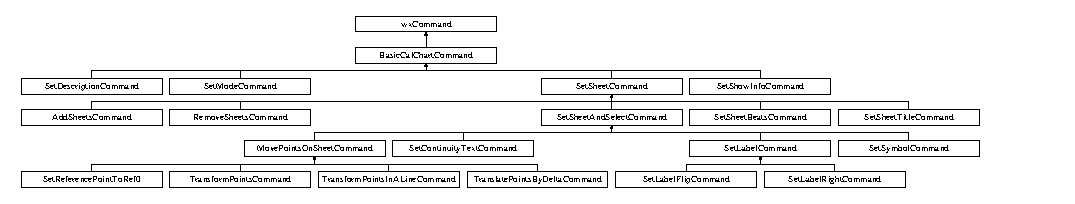
\includegraphics[height=2.296651cm]{a00018}
\end{center}
\end{figure}
\subsection*{Public Member Functions}
\begin{DoxyCompactItemize}
\item 
\hyperlink{a00018_a176cb9a986d1b043dd6d5350f3316bb9}{Basic\-Cal\-Chart\-Command} (\hyperlink{a00020}{Cal\-Chart\-Doc} \&doc, const wx\-String cmd\-Name)
\item 
virtual \hyperlink{a00018_a86f682185344e0b3eded54702d7b1f16}{$\sim$\-Basic\-Cal\-Chart\-Command} ()=0
\item 
virtual bool \hyperlink{a00018_a4e672c037f38626e4b8634c9613ea34e}{Do} ()
\item 
virtual bool \hyperlink{a00018_adfffde377bdc935cf06490667de1d7b6}{Undo} ()
\end{DoxyCompactItemize}
\subsection*{Protected Attributes}
\begin{DoxyCompactItemize}
\item 
\hyperlink{a00020}{Cal\-Chart\-Doc} \& \hyperlink{a00018_ab9f5e00f2b86c92e0051f56b889d1a13}{m\-Doc}
\end{DoxyCompactItemize}
\subsection*{Private Member Functions}
\begin{DoxyCompactItemize}
\item 
virtual void \hyperlink{a00018_ab6f65965601103020ea8276abf88313a}{Do\-Action} ()=0
\end{DoxyCompactItemize}
\subsection*{Private Attributes}
\begin{DoxyCompactItemize}
\item 
bool \hyperlink{a00018_a75aae02cbaadf5c37f31ec036078bc40}{m\-Doc\-Modified}
\item 
\hyperlink{a00046}{C\-C\-\_\-show} \hyperlink{a00018_a04e36485f183ef4967929432c0a08714}{m\-Snap\-Shot}
\end{DoxyCompactItemize}


\subsection{Constructor \& Destructor Documentation}
\hypertarget{a00018_a176cb9a986d1b043dd6d5350f3316bb9}{\index{Basic\-Cal\-Chart\-Command@{Basic\-Cal\-Chart\-Command}!Basic\-Cal\-Chart\-Command@{Basic\-Cal\-Chart\-Command}}
\index{Basic\-Cal\-Chart\-Command@{Basic\-Cal\-Chart\-Command}!BasicCalChartCommand@{Basic\-Cal\-Chart\-Command}}
\subsubsection[{Basic\-Cal\-Chart\-Command}]{\setlength{\rightskip}{0pt plus 5cm}Basic\-Cal\-Chart\-Command\-::\-Basic\-Cal\-Chart\-Command (
\begin{DoxyParamCaption}
\item[{{\bf Cal\-Chart\-Doc} \&}]{doc, }
\item[{const wx\-String}]{cmd\-Name}
\end{DoxyParamCaption}
)}}\label{a00018_a176cb9a986d1b043dd6d5350f3316bb9}
\hypertarget{a00018_a86f682185344e0b3eded54702d7b1f16}{\index{Basic\-Cal\-Chart\-Command@{Basic\-Cal\-Chart\-Command}!$\sim$\-Basic\-Cal\-Chart\-Command@{$\sim$\-Basic\-Cal\-Chart\-Command}}
\index{$\sim$\-Basic\-Cal\-Chart\-Command@{$\sim$\-Basic\-Cal\-Chart\-Command}!BasicCalChartCommand@{Basic\-Cal\-Chart\-Command}}
\subsubsection[{$\sim$\-Basic\-Cal\-Chart\-Command}]{\setlength{\rightskip}{0pt plus 5cm}Basic\-Cal\-Chart\-Command\-::$\sim$\-Basic\-Cal\-Chart\-Command (
\begin{DoxyParamCaption}
{}
\end{DoxyParamCaption}
)\hspace{0.3cm}{\ttfamily [pure virtual]}}}\label{a00018_a86f682185344e0b3eded54702d7b1f16}


\subsection{Member Function Documentation}
\hypertarget{a00018_a4e672c037f38626e4b8634c9613ea34e}{\index{Basic\-Cal\-Chart\-Command@{Basic\-Cal\-Chart\-Command}!Do@{Do}}
\index{Do@{Do}!BasicCalChartCommand@{Basic\-Cal\-Chart\-Command}}
\subsubsection[{Do}]{\setlength{\rightskip}{0pt plus 5cm}bool Basic\-Cal\-Chart\-Command\-::\-Do (
\begin{DoxyParamCaption}
{}
\end{DoxyParamCaption}
)\hspace{0.3cm}{\ttfamily [virtual]}}}\label{a00018_a4e672c037f38626e4b8634c9613ea34e}
\hypertarget{a00018_ab6f65965601103020ea8276abf88313a}{\index{Basic\-Cal\-Chart\-Command@{Basic\-Cal\-Chart\-Command}!Do\-Action@{Do\-Action}}
\index{Do\-Action@{Do\-Action}!BasicCalChartCommand@{Basic\-Cal\-Chart\-Command}}
\subsubsection[{Do\-Action}]{\setlength{\rightskip}{0pt plus 5cm}virtual void Basic\-Cal\-Chart\-Command\-::\-Do\-Action (
\begin{DoxyParamCaption}
{}
\end{DoxyParamCaption}
)\hspace{0.3cm}{\ttfamily [private]}, {\ttfamily [pure virtual]}}}\label{a00018_ab6f65965601103020ea8276abf88313a}


Implemented in \hyperlink{a00127_a1b03e239de9656b4fabe64f52ef502bb}{Set\-Label\-Command}, \hyperlink{a00124_a8545ed7f5c3ca572042c4a0abc8c2491}{Set\-Continuity\-Text\-Command}, \hyperlink{a00137_ac01aa3b3a02f3a8db5b16e9cbb1c3228}{Set\-Symbol\-Command}, \hyperlink{a00112_a2339b105a336b22d59771534a3f4a304}{Move\-Points\-On\-Sheet\-Command}, \hyperlink{a00132_ae017079a0a6c65222f10968fad8fc082}{Set\-Sheet\-And\-Select\-Command}, \hyperlink{a00122_ac289d6c5166a7139fa0c61c664d1710e}{Remove\-Sheets\-Command}, \hyperlink{a00001_aba46cac1335e29189a9aaf5b50d3f364}{Add\-Sheets\-Command}, \hyperlink{a00133_a9efb63e15dae7c253792ae214feda42e}{Set\-Sheet\-Beats\-Command}, \hyperlink{a00135_ab2e45d322adbc00b829917145585e152}{Set\-Sheet\-Title\-Command}, \hyperlink{a00134_a027700275d409b94185dfb3aa2d792bb}{Set\-Sheet\-Command}, \hyperlink{a00136_abf979162c4c398c5f11057410f3c2bc2}{Set\-Show\-Info\-Command}, \hyperlink{a00130_aa9a96b69185714f4acfa18ae5812cbcf}{Set\-Mode\-Command}, and \hyperlink{a00125_a1e24fd27d87d38070e1823095d396d28}{Set\-Description\-Command}.

\hypertarget{a00018_adfffde377bdc935cf06490667de1d7b6}{\index{Basic\-Cal\-Chart\-Command@{Basic\-Cal\-Chart\-Command}!Undo@{Undo}}
\index{Undo@{Undo}!BasicCalChartCommand@{Basic\-Cal\-Chart\-Command}}
\subsubsection[{Undo}]{\setlength{\rightskip}{0pt plus 5cm}bool Basic\-Cal\-Chart\-Command\-::\-Undo (
\begin{DoxyParamCaption}
{}
\end{DoxyParamCaption}
)\hspace{0.3cm}{\ttfamily [virtual]}}}\label{a00018_adfffde377bdc935cf06490667de1d7b6}


\subsection{Member Data Documentation}
\hypertarget{a00018_ab9f5e00f2b86c92e0051f56b889d1a13}{\index{Basic\-Cal\-Chart\-Command@{Basic\-Cal\-Chart\-Command}!m\-Doc@{m\-Doc}}
\index{m\-Doc@{m\-Doc}!BasicCalChartCommand@{Basic\-Cal\-Chart\-Command}}
\subsubsection[{m\-Doc}]{\setlength{\rightskip}{0pt plus 5cm}{\bf Cal\-Chart\-Doc}\& Basic\-Cal\-Chart\-Command\-::m\-Doc\hspace{0.3cm}{\ttfamily [protected]}}}\label{a00018_ab9f5e00f2b86c92e0051f56b889d1a13}
\hypertarget{a00018_a75aae02cbaadf5c37f31ec036078bc40}{\index{Basic\-Cal\-Chart\-Command@{Basic\-Cal\-Chart\-Command}!m\-Doc\-Modified@{m\-Doc\-Modified}}
\index{m\-Doc\-Modified@{m\-Doc\-Modified}!BasicCalChartCommand@{Basic\-Cal\-Chart\-Command}}
\subsubsection[{m\-Doc\-Modified}]{\setlength{\rightskip}{0pt plus 5cm}bool Basic\-Cal\-Chart\-Command\-::m\-Doc\-Modified\hspace{0.3cm}{\ttfamily [private]}}}\label{a00018_a75aae02cbaadf5c37f31ec036078bc40}
\hypertarget{a00018_a04e36485f183ef4967929432c0a08714}{\index{Basic\-Cal\-Chart\-Command@{Basic\-Cal\-Chart\-Command}!m\-Snap\-Shot@{m\-Snap\-Shot}}
\index{m\-Snap\-Shot@{m\-Snap\-Shot}!BasicCalChartCommand@{Basic\-Cal\-Chart\-Command}}
\subsubsection[{m\-Snap\-Shot}]{\setlength{\rightskip}{0pt plus 5cm}{\bf C\-C\-\_\-show} Basic\-Cal\-Chart\-Command\-::m\-Snap\-Shot\hspace{0.3cm}{\ttfamily [private]}}}\label{a00018_a04e36485f183ef4967929432c0a08714}


The documentation for this class was generated from the following files\-:\begin{DoxyCompactItemize}
\item 
src/\hyperlink{a00183}{cc\-\_\-command.\-h}\item 
src/\hyperlink{a00182}{cc\-\_\-command.\-cpp}\end{DoxyCompactItemize}

\hypertarget{a00019}{\section{Cal\-Chart\-App Class Reference}
\label{a00019}\index{Cal\-Chart\-App@{Cal\-Chart\-App}}
}


The Calchart Application.  




{\ttfamily \#include $<$calchartapp.\-h$>$}

Inheritance diagram for Cal\-Chart\-App\-:\begin{figure}[H]
\begin{center}
\leavevmode
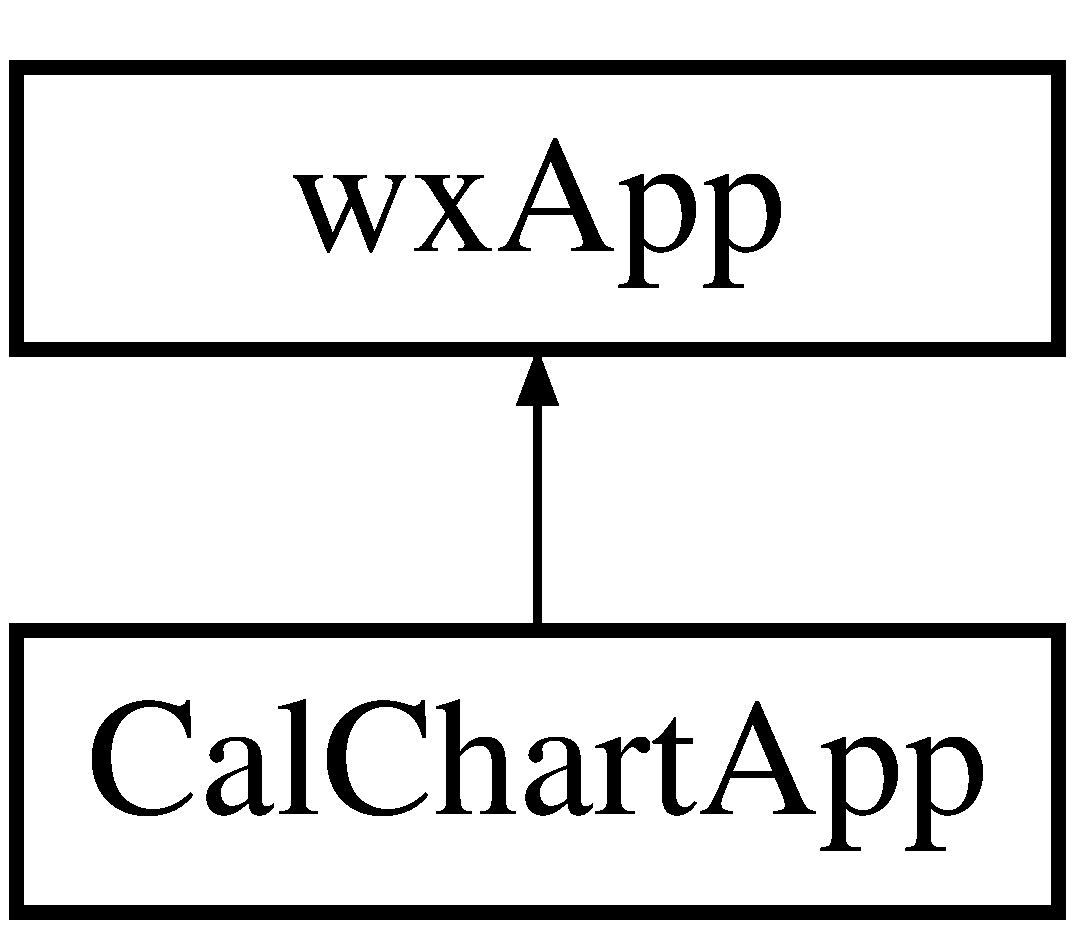
\includegraphics[height=2.000000cm]{a00019}
\end{center}
\end{figure}
\subsection*{Public Member Functions}
\begin{DoxyCompactItemize}
\item 
virtual bool \hyperlink{a00019_a18be3b3d0fad5cca9d071c8db6d535cc}{On\-Init} ()
\begin{DoxyCompactList}\small\item\em Initializes the application. \end{DoxyCompactList}\item 
virtual void \hyperlink{a00019_a0dca14f2ffaf9038c2b11df641d46bd6}{Mac\-Open\-File} (const wx\-String \&file\-Name)
\begin{DoxyCompactList}\small\item\em T\-O\-D\-O -\/ I'm not a mac user... \end{DoxyCompactList}\item 
int \hyperlink{a00019_af5b65edc5a8a3d066f798406cb695a3e}{On\-Exit} ()
\begin{DoxyCompactList}\small\item\em Cleans up the application immediately before exiting. \end{DoxyCompactList}\item 
\hyperlink{a00236_a39f2aa1ac0d2da59ef7f3e58b13f44d2}{Show\-Mode\-List} \& \hyperlink{a00019_ae786827951680706302792f8efff7744}{Get\-Mode\-List} ()
\end{DoxyCompactItemize}
\subsection*{Private Attributes}
\begin{DoxyCompactItemize}
\item 
\hyperlink{a00236_a39f2aa1ac0d2da59ef7f3e58b13f44d2}{Show\-Mode\-List} \hyperlink{a00019_a1b1b26f2dfd6c8c9b3b4197a76a5508f}{m\-Mode\-List}
\item 
wx\-Doc\-Manager $\ast$ \hyperlink{a00019_a57de14625ab8d1f57c4bdc02e0a9dd8b}{m\-Doc\-Manager}
\begin{DoxyCompactList}\small\item\em Handles the opening/saving/viewing of Cal\-Chart-\/associated files. \end{DoxyCompactList}\end{DoxyCompactItemize}


\subsection{Detailed Description}
The Calchart Application. 

This class (a wx\-Widgets application) functions as the starting point for the Cal\-Chart program. When you start up the Cal\-Chart program, the \hyperlink{a00019_a18be3b3d0fad5cca9d071c8db6d535cc}{On\-Init()} method of \hyperlink{a00019}{Cal\-Chart\-App} is called, and when you close the program, the \hyperlink{a00019_af5b65edc5a8a3d066f798406cb695a3e}{On\-Exit()} method is called. This class is not drawn (so it is invisible) to the user, but when \hyperlink{a00019_a18be3b3d0fad5cca9d071c8db6d535cc}{On\-Init()} is called (that is, when the user starts up a new Cal\-Chart instance), \hyperlink{a00019}{Cal\-Chart\-App} creates a frame that I\-S visible to the user, and the user can use that frame to view and edit shows. 

\subsection{Member Function Documentation}
\hypertarget{a00019_ae786827951680706302792f8efff7744}{\index{Cal\-Chart\-App@{Cal\-Chart\-App}!Get\-Mode\-List@{Get\-Mode\-List}}
\index{Get\-Mode\-List@{Get\-Mode\-List}!CalChartApp@{Cal\-Chart\-App}}
\subsubsection[{Get\-Mode\-List}]{\setlength{\rightskip}{0pt plus 5cm}{\bf Show\-Mode\-List}\& Cal\-Chart\-App\-::\-Get\-Mode\-List (
\begin{DoxyParamCaption}
{}
\end{DoxyParamCaption}
)\hspace{0.3cm}{\ttfamily [inline]}}}\label{a00019_ae786827951680706302792f8efff7744}
\hypertarget{a00019_a0dca14f2ffaf9038c2b11df641d46bd6}{\index{Cal\-Chart\-App@{Cal\-Chart\-App}!Mac\-Open\-File@{Mac\-Open\-File}}
\index{Mac\-Open\-File@{Mac\-Open\-File}!CalChartApp@{Cal\-Chart\-App}}
\subsubsection[{Mac\-Open\-File}]{\setlength{\rightskip}{0pt plus 5cm}void Cal\-Chart\-App\-::\-Mac\-Open\-File (
\begin{DoxyParamCaption}
\item[{const wx\-String \&}]{file\-Name}
\end{DoxyParamCaption}
)\hspace{0.3cm}{\ttfamily [virtual]}}}\label{a00019_a0dca14f2ffaf9038c2b11df641d46bd6}


T\-O\-D\-O -\/ I'm not a mac user... 


\begin{DoxyParams}{Parameters}
{\em file\-Name} & The name of the file to open. \\
\hline
\end{DoxyParams}
\hypertarget{a00019_af5b65edc5a8a3d066f798406cb695a3e}{\index{Cal\-Chart\-App@{Cal\-Chart\-App}!On\-Exit@{On\-Exit}}
\index{On\-Exit@{On\-Exit}!CalChartApp@{Cal\-Chart\-App}}
\subsubsection[{On\-Exit}]{\setlength{\rightskip}{0pt plus 5cm}int Cal\-Chart\-App\-::\-On\-Exit (
\begin{DoxyParamCaption}
{}
\end{DoxyParamCaption}
)}}\label{a00019_af5b65edc5a8a3d066f798406cb695a3e}


Cleans up the application immediately before exiting. 

This method is called when the program is closed. It performs cleanup. \hypertarget{a00019_a18be3b3d0fad5cca9d071c8db6d535cc}{\index{Cal\-Chart\-App@{Cal\-Chart\-App}!On\-Init@{On\-Init}}
\index{On\-Init@{On\-Init}!CalChartApp@{Cal\-Chart\-App}}
\subsubsection[{On\-Init}]{\setlength{\rightskip}{0pt plus 5cm}bool Cal\-Chart\-App\-::\-On\-Init (
\begin{DoxyParamCaption}
{}
\end{DoxyParamCaption}
)\hspace{0.3cm}{\ttfamily [virtual]}}}\label{a00019_a18be3b3d0fad5cca9d071c8db6d535cc}


Initializes the application. 

This method is called when the program starts. It is responsible for setting up the frame to which Cal\-Chart is drawn (thereby making the program visible to the user) and for linking that frame to a wx\-Doc\-Manager that understands the Cal\-Chart show file, including how to open it, save it, and display it. The frame uses the wx\-Doc\-Manager to properly display the Cal\-Chart show to the user. 

\subsection{Member Data Documentation}
\hypertarget{a00019_a57de14625ab8d1f57c4bdc02e0a9dd8b}{\index{Cal\-Chart\-App@{Cal\-Chart\-App}!m\-Doc\-Manager@{m\-Doc\-Manager}}
\index{m\-Doc\-Manager@{m\-Doc\-Manager}!CalChartApp@{Cal\-Chart\-App}}
\subsubsection[{m\-Doc\-Manager}]{\setlength{\rightskip}{0pt plus 5cm}wx\-Doc\-Manager$\ast$ Cal\-Chart\-App\-::m\-Doc\-Manager\hspace{0.3cm}{\ttfamily [private]}}}\label{a00019_a57de14625ab8d1f57c4bdc02e0a9dd8b}


Handles the opening/saving/viewing of Cal\-Chart-\/associated files. 

The document manager associated with Cal\-Chart. This is responsible for understanding each of the file types associated with Cal\-Chart -\/ that is, it must understand how to view, save, and open files like the .shw file. \hypertarget{a00019_a1b1b26f2dfd6c8c9b3b4197a76a5508f}{\index{Cal\-Chart\-App@{Cal\-Chart\-App}!m\-Mode\-List@{m\-Mode\-List}}
\index{m\-Mode\-List@{m\-Mode\-List}!CalChartApp@{Cal\-Chart\-App}}
\subsubsection[{m\-Mode\-List}]{\setlength{\rightskip}{0pt plus 5cm}{\bf Show\-Mode\-List} Cal\-Chart\-App\-::m\-Mode\-List\hspace{0.3cm}{\ttfamily [private]}}}\label{a00019_a1b1b26f2dfd6c8c9b3b4197a76a5508f}


The documentation for this class was generated from the following files\-:\begin{DoxyCompactItemize}
\item 
src/\hyperlink{a00179}{calchartapp.\-h}\item 
src/\hyperlink{a00178}{calchartapp.\-cpp}\end{DoxyCompactItemize}

\hypertarget{a00020}{\section{Cal\-Chart\-Doc Class Reference}
\label{a00020}\index{Cal\-Chart\-Doc@{Cal\-Chart\-Doc}}
}


{\ttfamily \#include $<$calchartdoc.\-h$>$}

Inheritance diagram for Cal\-Chart\-Doc\-:\begin{figure}[H]
\begin{center}
\leavevmode
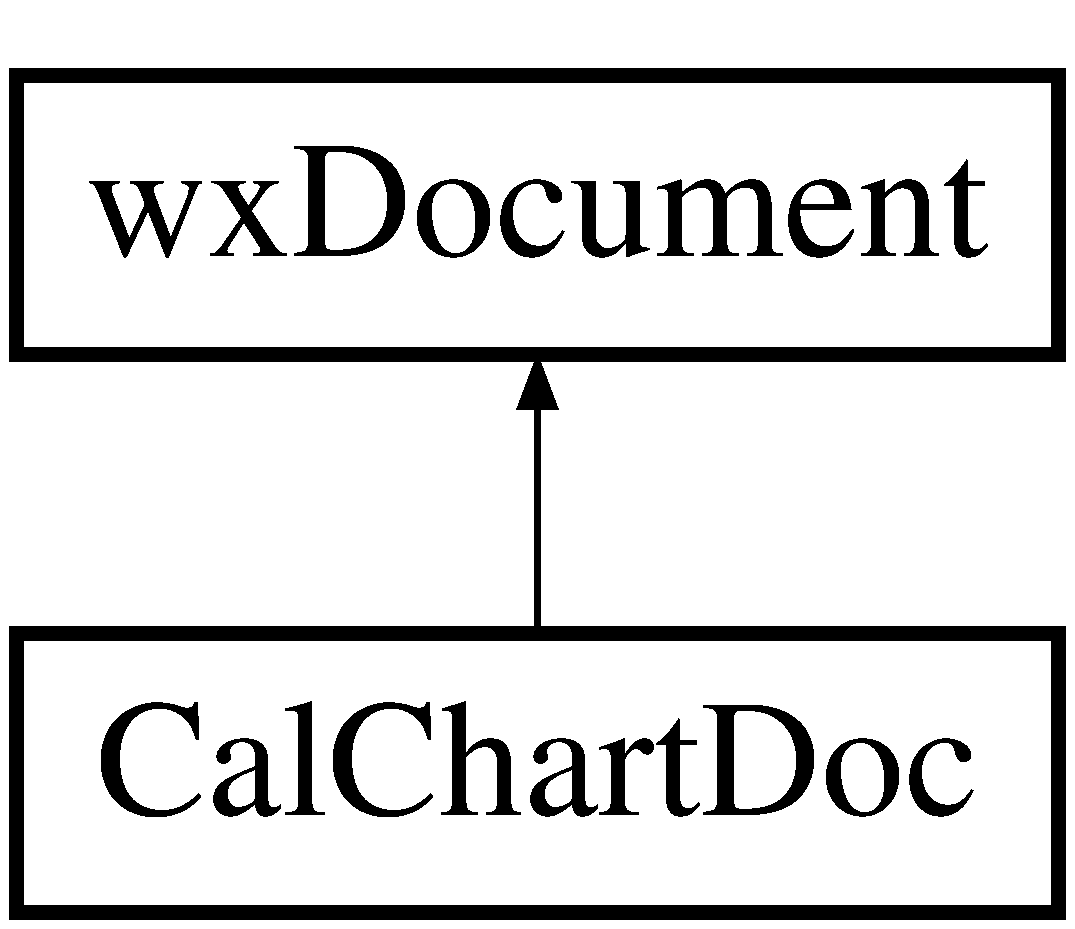
\includegraphics[height=2.000000cm]{a00020}
\end{center}
\end{figure}
\subsection*{Classes}
\begin{DoxyCompactItemize}
\item 
class \hyperlink{a00016}{Auto\-Save\-Timer}
\end{DoxyCompactItemize}
\subsection*{Public Types}
\begin{DoxyCompactItemize}
\item 
typedef std\-::vector$<$ \hyperlink{a00045}{C\-C\-\_\-sheet} $>$ \hyperlink{a00020_ab378b0e2a08984cfda6487b5161e520c}{C\-C\-\_\-sheet\-\_\-container\-\_\-t}
\item 
typedef \\*
C\-C\-\_\-sheet\-\_\-container\-\_\-t\-::iterator \hyperlink{a00020_a36548f14d6c85b0abee6f2956dbe4689}{C\-C\-\_\-sheet\-\_\-iterator\-\_\-t}
\item 
typedef \\*
C\-C\-\_\-sheet\-\_\-container\-\_\-t\-::const\-\_\-iterator \hyperlink{a00020_a40ea5298b58fb5f3b5f648e6ef36a286}{const\-\_\-\-C\-C\-\_\-sheet\-\_\-iterator\-\_\-t}
\end{DoxyCompactItemize}
\subsection*{Public Member Functions}
\begin{DoxyCompactItemize}
\item 
\hyperlink{a00020_a8a872d648b6e3b4f266174a0acfdc9fc}{Cal\-Chart\-Doc} ()
\item 
virtual \hyperlink{a00020_a14812da32f9bd5e002b6b118f7b010da}{$\sim$\-Cal\-Chart\-Doc} ()
\item 
virtual bool \hyperlink{a00020_a0e877ef3a12b3517e55c2f9c1289e4f6}{On\-Open\-Document} (const wx\-String \&filename)
\item 
virtual bool \hyperlink{a00020_a4b63a837f554888d1da135139e01b14d}{On\-Close\-Document} ()
\item 
virtual bool \hyperlink{a00020_a381f76c44e5e5ba713d4976fef1869af}{On\-New\-Document} ()
\item 
virtual bool \hyperlink{a00020_a345b07be3b8de12a585c1d1b94979470}{On\-Save\-Document} (const wx\-String \&filename)
\item 
virtual void \hyperlink{a00020_a416ddefdb179e2c5a8bfcb37c9478fe4}{Modify} (bool b)
\item 
virtual wx\-Output\-Stream \& \hyperlink{a00020_a54e00f93eb412376423397723fc65598}{Save\-Object} (wx\-Output\-Stream \&stream)
\item 
virtual wx\-Input\-Stream \& \hyperlink{a00020_ab7865ea2508bf7164e31a09af935e064}{Load\-Object} (wx\-Input\-Stream \&stream)
\item 
wx\-String \hyperlink{a00020_a1a6a217147ecfd305e4a26c5f9b80c2b}{Import\-Continuity} (const wx\-String \&file)
\item 
void \hyperlink{a00020_a95afc07cf9b63a410fc0bf374e1ee497}{Flush\-All\-Text\-Windows} ()
\item 
boost\-::shared\-\_\-ptr$<$ \hyperlink{a00010}{Animation} $>$ \hyperlink{a00020_a7da13b0aa139317724bfe184f13f7f4f}{New\-Animation} (\hyperlink{a00195_aef08fe65401b34c561d7d6fc0ff39b60}{Notify\-Status} notify\-Status, \hyperlink{a00195_a9f9c725e3e1c76c65ddb676bf591d49b}{Notify\-Error\-List} notify\-Error\-List)
\item 
void \hyperlink{a00020_af7fe59d238be4bb9c153cd3e25b12a84}{Setup\-New\-Show} ()
\item 
const std\-::string \& \hyperlink{a00020_a58ec7334fcd1caec3d4e6a4052ebf0c5}{Get\-Descr} () const 
\item 
void \hyperlink{a00020_a0e1bc530f6bc782c906d3f618f3c82b9}{Set\-Descr} (const std\-::string \&newdescr)
\item 
unsigned short \hyperlink{a00020_a30d9d301120a9403df378ee303aebf59}{Get\-Num\-Sheets} () const 
\item 
\hyperlink{a00020_a36548f14d6c85b0abee6f2956dbe4689}{C\-C\-\_\-sheet\-\_\-iterator\-\_\-t} \hyperlink{a00020_a22498e3126c272da81dcc1d0fa182910}{Get\-Sheet\-Begin} ()
\item 
\hyperlink{a00020_a40ea5298b58fb5f3b5f648e6ef36a286}{const\-\_\-\-C\-C\-\_\-sheet\-\_\-iterator\-\_\-t} \hyperlink{a00020_a7fb89b997fae2ae0289ecd27726aa575}{Get\-Sheet\-Begin} () const 
\item 
\hyperlink{a00020_a36548f14d6c85b0abee6f2956dbe4689}{C\-C\-\_\-sheet\-\_\-iterator\-\_\-t} \hyperlink{a00020_ac78d213242b2e2ef3d325408e9b1e833}{Get\-Sheet\-End} ()
\item 
\hyperlink{a00020_a40ea5298b58fb5f3b5f648e6ef36a286}{const\-\_\-\-C\-C\-\_\-sheet\-\_\-iterator\-\_\-t} \hyperlink{a00020_a674bbc27dcb20e531990f0cd805af30f}{Get\-Sheet\-End} () const 
\item 
\hyperlink{a00020_a40ea5298b58fb5f3b5f648e6ef36a286}{const\-\_\-\-C\-C\-\_\-sheet\-\_\-iterator\-\_\-t} \hyperlink{a00020_a216aa095052dd49768df6f3cd2081c0f}{Get\-Nth\-Sheet} (unsigned n) const 
\item 
\hyperlink{a00020_a36548f14d6c85b0abee6f2956dbe4689}{C\-C\-\_\-sheet\-\_\-iterator\-\_\-t} \hyperlink{a00020_a376aafc4d2807f46224a1d22bf53c19c}{Get\-Nth\-Sheet} (unsigned n)
\item 
\hyperlink{a00020_a40ea5298b58fb5f3b5f648e6ef36a286}{const\-\_\-\-C\-C\-\_\-sheet\-\_\-iterator\-\_\-t} \hyperlink{a00020_ad5fc3c4cd218407e379fa46e035c4468}{Get\-Current\-Sheet} () const 
\item 
\hyperlink{a00020_a36548f14d6c85b0abee6f2956dbe4689}{C\-C\-\_\-sheet\-\_\-iterator\-\_\-t} \hyperlink{a00020_a22e2a3326eb62ee50daca0b206d72da5}{Get\-Current\-Sheet} ()
\item 
unsigned \hyperlink{a00020_a615c0173959b086005891bef66f51ced}{Get\-Current\-Sheet\-Num} () const 
\item 
void \hyperlink{a00020_ae455fd80d3ee97a29789d238801a60bb}{Set\-Current\-Sheet} (unsigned n)
\item 
\hyperlink{a00020_ab378b0e2a08984cfda6487b5161e520c}{C\-C\-\_\-sheet\-\_\-container\-\_\-t} \hyperlink{a00020_a852e785dd0b4ea390a795ed900aaf8cd}{Remove\-Nth\-Sheet} (unsigned sheetidx)
\item 
void \hyperlink{a00020_a3db922015ff5d01bd29f6b779632e0b0}{Delete\-Nth\-Sheet} (unsigned sheetidx)
\item 
void \hyperlink{a00020_a572a00b153485ce85c34262d66bdfffe}{Insert\-Sheet\-Internal} (const \hyperlink{a00045}{C\-C\-\_\-sheet} \&nsheet, unsigned sheetidx)
\item 
void \hyperlink{a00020_a91888ec48bb8b757d4a283a7d9b9ddaa}{Insert\-Sheet\-Internal} (const \hyperlink{a00020_ab378b0e2a08984cfda6487b5161e520c}{C\-C\-\_\-sheet\-\_\-container\-\_\-t} \&nsheet, unsigned sheetidx)
\item 
void \hyperlink{a00020_aa53e408dc4207c9ba0cf8de3eadf6bf5}{Insert\-Sheet} (const \hyperlink{a00045}{C\-C\-\_\-sheet} \&nsheet, unsigned sheetidx)
\item 
unsigned short \hyperlink{a00020_a5df09716c299172f2e8a99b1a90267e5}{Get\-Num\-Points} () const 
\item 
void \hyperlink{a00020_a3b373d2e691b8a5f2f719f4eee37f3dd}{Set\-Num\-Points} (unsigned num, unsigned columns)
\item 
bool \hyperlink{a00020_aa78b0dc2aee7cc0a66ddbd41c9231093}{Relabel\-Sheets} (unsigned sht)
\item 
std\-::string \hyperlink{a00020_a661207ede21362e43acb5399755115a5}{Get\-Point\-Label} (unsigned i) const 
\item 
void \hyperlink{a00020_a898de26e0833809c2df3870b1e800834}{Set\-Point\-Label} (const std\-::vector$<$ std\-::string $>$ \&labels)
\item 
const std\-::vector$<$ std\-::string $>$ \& \hyperlink{a00020_a3733a8b0ba76987f61b22a5a5fa1f05b}{Get\-Point\-Labels} () const 
\item 
bool \hyperlink{a00020_a79e6fc4893b17057221f0b6f7cf259cb}{Select\-All} ()
\item 
bool \hyperlink{a00020_aca913f542da51caebfff9efa14adbe94}{Unselect\-All} ()
\item 
void \hyperlink{a00020_af33d8ef299f4bf47949078f2a505c505}{Add\-To\-Selection} (const \hyperlink{a00214_aaec86d4bb87e1e6f0b60e6e551c5e570}{Selection\-List} \&sl)
\item 
void \hyperlink{a00020_afa0213a64648754e4a40fe0310ae795c}{Set\-Selection} (const \hyperlink{a00214_aaec86d4bb87e1e6f0b60e6e551c5e570}{Selection\-List} \&sl)
\item 
void \hyperlink{a00020_a006550de9209e5e3785d92d2e3101f97}{Remove\-From\-Selection} (const \hyperlink{a00214_aaec86d4bb87e1e6f0b60e6e551c5e570}{Selection\-List} \&sl)
\item 
void \hyperlink{a00020_ad7065faea6e297d81be3de222a63900b}{Toggle\-Selection} (const \hyperlink{a00214_aaec86d4bb87e1e6f0b60e6e551c5e570}{Selection\-List} \&sl)
\item 
void \hyperlink{a00020_a48d9d1df2b7f47503bacc610f432d48a}{Select\-With\-Lasso} (const \hyperlink{a00033}{C\-C\-\_\-lasso} \&lasso, bool toggle\-Selected, unsigned ref)
\item 
bool \hyperlink{a00020_a2666154ab00c2127fb8740a77ae04856}{Is\-Selected} (unsigned i) const 
\item 
const \hyperlink{a00214_aaec86d4bb87e1e6f0b60e6e551c5e570}{Selection\-List} \& \hyperlink{a00020_a9916a116564564d7c3e90021dabb86e4}{Get\-Selection\-List} () const 
\item 
const \hyperlink{a00140}{Show\-Mode} \& \hyperlink{a00020_a231e6c0aeefd7afec51a49db5d1349af}{Get\-Mode} () const 
\item 
void \hyperlink{a00020_a72e6705427c5773fcd1df68c95f2e9d2}{Set\-Mode} (const \hyperlink{a00140}{Show\-Mode} $\ast$m)
\end{DoxyCompactItemize}
\subsection*{Private Member Functions}
\begin{DoxyCompactItemize}
\item 
{\footnotesize template$<$typename T $>$ }\\T \& \hyperlink{a00020_aabfbb31b7de0e12f2e27995ac2d1209c}{Load\-Object\-Generic} (T \&stream)
\item 
{\footnotesize template$<$typename T $>$ }\\T \& \hyperlink{a00020_a62d5b478a611035540c73debd4acd931}{Save\-Object\-Generic} (T \&stream)
\item 
{\footnotesize template$<$typename T $>$ }\\T \& \hyperlink{a00020_a1096edf60a2763abbf3515cdd50a03ae}{Save\-Object\-Internal} (T \&stream)
\item 
void \hyperlink{a00020_a12175e69b77c48480c4e3ddd63917798}{Autosave} ()
\item 
\hyperlink{a00046}{C\-C\-\_\-show} \hyperlink{a00020_acf62d914a19a769892d16ee3648ac94c}{Show\-Snap\-Shot} () const 
\item 
void \hyperlink{a00020_a62683f9baddb64becf2e233c30fc202a}{Restore\-Snap\-Shot} (const \hyperlink{a00046}{C\-C\-\_\-show} \&snapshot)
\item 
{\footnotesize template$<$$>$ }\\wx\-F\-File\-Output\-Stream \& \hyperlink{a00020_ae810c29cd5c949ba61017646cd5ce093}{Save\-Object\-Internal} (wx\-F\-File\-Output\-Stream \&stream)
\end{DoxyCompactItemize}
\subsection*{Static Private Member Functions}
\begin{DoxyCompactItemize}
\item 
static wx\-String \hyperlink{a00020_a7945816f5d04a38baeef9c503e3f4402}{Translate\-Name\-To\-Autosave\-Name} (const wx\-String \&name)
\end{DoxyCompactItemize}
\subsection*{Private Attributes}
\begin{DoxyCompactItemize}
\item 
std\-::unique\-\_\-ptr$<$ \hyperlink{a00046}{C\-C\-\_\-show} $>$ \hyperlink{a00020_a42ef10531f8c3d4a0bedc609fdf66936}{m\-Show}
\item 
const \hyperlink{a00140}{Show\-Mode} $\ast$ \hyperlink{a00020_ae511411f0afc9c334fea3f2df435e893}{m\-Mode}
\item 
\hyperlink{a00016}{Auto\-Save\-Timer} \hyperlink{a00020_a74f920890947909b3c2a8d8cac6d1f78}{m\-Timer}
\end{DoxyCompactItemize}
\subsection*{Friends}
\begin{DoxyCompactItemize}
\item 
class \hyperlink{a00020_abdbcdfbd8a7d6cea4cf9e05b947e47d0}{Basic\-Cal\-Chart\-Command}
\end{DoxyCompactItemize}


\subsection{Member Typedef Documentation}
\hypertarget{a00020_ab378b0e2a08984cfda6487b5161e520c}{\index{Cal\-Chart\-Doc@{Cal\-Chart\-Doc}!C\-C\-\_\-sheet\-\_\-container\-\_\-t@{C\-C\-\_\-sheet\-\_\-container\-\_\-t}}
\index{C\-C\-\_\-sheet\-\_\-container\-\_\-t@{C\-C\-\_\-sheet\-\_\-container\-\_\-t}!CalChartDoc@{Cal\-Chart\-Doc}}
\subsubsection[{C\-C\-\_\-sheet\-\_\-container\-\_\-t}]{\setlength{\rightskip}{0pt plus 5cm}typedef std\-::vector$<${\bf C\-C\-\_\-sheet}$>$ {\bf Cal\-Chart\-Doc\-::\-C\-C\-\_\-sheet\-\_\-container\-\_\-t}}}\label{a00020_ab378b0e2a08984cfda6487b5161e520c}
\hypertarget{a00020_a36548f14d6c85b0abee6f2956dbe4689}{\index{Cal\-Chart\-Doc@{Cal\-Chart\-Doc}!C\-C\-\_\-sheet\-\_\-iterator\-\_\-t@{C\-C\-\_\-sheet\-\_\-iterator\-\_\-t}}
\index{C\-C\-\_\-sheet\-\_\-iterator\-\_\-t@{C\-C\-\_\-sheet\-\_\-iterator\-\_\-t}!CalChartDoc@{Cal\-Chart\-Doc}}
\subsubsection[{C\-C\-\_\-sheet\-\_\-iterator\-\_\-t}]{\setlength{\rightskip}{0pt plus 5cm}typedef C\-C\-\_\-sheet\-\_\-container\-\_\-t\-::iterator {\bf Cal\-Chart\-Doc\-::\-C\-C\-\_\-sheet\-\_\-iterator\-\_\-t}}}\label{a00020_a36548f14d6c85b0abee6f2956dbe4689}
\hypertarget{a00020_a40ea5298b58fb5f3b5f648e6ef36a286}{\index{Cal\-Chart\-Doc@{Cal\-Chart\-Doc}!const\-\_\-\-C\-C\-\_\-sheet\-\_\-iterator\-\_\-t@{const\-\_\-\-C\-C\-\_\-sheet\-\_\-iterator\-\_\-t}}
\index{const\-\_\-\-C\-C\-\_\-sheet\-\_\-iterator\-\_\-t@{const\-\_\-\-C\-C\-\_\-sheet\-\_\-iterator\-\_\-t}!CalChartDoc@{Cal\-Chart\-Doc}}
\subsubsection[{const\-\_\-\-C\-C\-\_\-sheet\-\_\-iterator\-\_\-t}]{\setlength{\rightskip}{0pt plus 5cm}typedef C\-C\-\_\-sheet\-\_\-container\-\_\-t\-::const\-\_\-iterator {\bf Cal\-Chart\-Doc\-::const\-\_\-\-C\-C\-\_\-sheet\-\_\-iterator\-\_\-t}}}\label{a00020_a40ea5298b58fb5f3b5f648e6ef36a286}


\subsection{Constructor \& Destructor Documentation}
\hypertarget{a00020_a8a872d648b6e3b4f266174a0acfdc9fc}{\index{Cal\-Chart\-Doc@{Cal\-Chart\-Doc}!Cal\-Chart\-Doc@{Cal\-Chart\-Doc}}
\index{Cal\-Chart\-Doc@{Cal\-Chart\-Doc}!CalChartDoc@{Cal\-Chart\-Doc}}
\subsubsection[{Cal\-Chart\-Doc}]{\setlength{\rightskip}{0pt plus 5cm}Cal\-Chart\-Doc\-::\-Cal\-Chart\-Doc (
\begin{DoxyParamCaption}
{}
\end{DoxyParamCaption}
)}}\label{a00020_a8a872d648b6e3b4f266174a0acfdc9fc}
\hypertarget{a00020_a14812da32f9bd5e002b6b118f7b010da}{\index{Cal\-Chart\-Doc@{Cal\-Chart\-Doc}!$\sim$\-Cal\-Chart\-Doc@{$\sim$\-Cal\-Chart\-Doc}}
\index{$\sim$\-Cal\-Chart\-Doc@{$\sim$\-Cal\-Chart\-Doc}!CalChartDoc@{Cal\-Chart\-Doc}}
\subsubsection[{$\sim$\-Cal\-Chart\-Doc}]{\setlength{\rightskip}{0pt plus 5cm}Cal\-Chart\-Doc\-::$\sim$\-Cal\-Chart\-Doc (
\begin{DoxyParamCaption}
{}
\end{DoxyParamCaption}
)\hspace{0.3cm}{\ttfamily [virtual]}}}\label{a00020_a14812da32f9bd5e002b6b118f7b010da}


\subsection{Member Function Documentation}
\hypertarget{a00020_af33d8ef299f4bf47949078f2a505c505}{\index{Cal\-Chart\-Doc@{Cal\-Chart\-Doc}!Add\-To\-Selection@{Add\-To\-Selection}}
\index{Add\-To\-Selection@{Add\-To\-Selection}!CalChartDoc@{Cal\-Chart\-Doc}}
\subsubsection[{Add\-To\-Selection}]{\setlength{\rightskip}{0pt plus 5cm}void Cal\-Chart\-Doc\-::\-Add\-To\-Selection (
\begin{DoxyParamCaption}
\item[{const {\bf Selection\-List} \&}]{sl}
\end{DoxyParamCaption}
)}}\label{a00020_af33d8ef299f4bf47949078f2a505c505}
\hypertarget{a00020_a12175e69b77c48480c4e3ddd63917798}{\index{Cal\-Chart\-Doc@{Cal\-Chart\-Doc}!Autosave@{Autosave}}
\index{Autosave@{Autosave}!CalChartDoc@{Cal\-Chart\-Doc}}
\subsubsection[{Autosave}]{\setlength{\rightskip}{0pt plus 5cm}void Cal\-Chart\-Doc\-::\-Autosave (
\begin{DoxyParamCaption}
{}
\end{DoxyParamCaption}
)\hspace{0.3cm}{\ttfamily [private]}}}\label{a00020_a12175e69b77c48480c4e3ddd63917798}
\hypertarget{a00020_a3db922015ff5d01bd29f6b779632e0b0}{\index{Cal\-Chart\-Doc@{Cal\-Chart\-Doc}!Delete\-Nth\-Sheet@{Delete\-Nth\-Sheet}}
\index{Delete\-Nth\-Sheet@{Delete\-Nth\-Sheet}!CalChartDoc@{Cal\-Chart\-Doc}}
\subsubsection[{Delete\-Nth\-Sheet}]{\setlength{\rightskip}{0pt plus 5cm}void Cal\-Chart\-Doc\-::\-Delete\-Nth\-Sheet (
\begin{DoxyParamCaption}
\item[{unsigned}]{sheetidx}
\end{DoxyParamCaption}
)}}\label{a00020_a3db922015ff5d01bd29f6b779632e0b0}
\hypertarget{a00020_a95afc07cf9b63a410fc0bf374e1ee497}{\index{Cal\-Chart\-Doc@{Cal\-Chart\-Doc}!Flush\-All\-Text\-Windows@{Flush\-All\-Text\-Windows}}
\index{Flush\-All\-Text\-Windows@{Flush\-All\-Text\-Windows}!CalChartDoc@{Cal\-Chart\-Doc}}
\subsubsection[{Flush\-All\-Text\-Windows}]{\setlength{\rightskip}{0pt plus 5cm}void Cal\-Chart\-Doc\-::\-Flush\-All\-Text\-Windows (
\begin{DoxyParamCaption}
{}
\end{DoxyParamCaption}
)}}\label{a00020_a95afc07cf9b63a410fc0bf374e1ee497}
\hypertarget{a00020_ad5fc3c4cd218407e379fa46e035c4468}{\index{Cal\-Chart\-Doc@{Cal\-Chart\-Doc}!Get\-Current\-Sheet@{Get\-Current\-Sheet}}
\index{Get\-Current\-Sheet@{Get\-Current\-Sheet}!CalChartDoc@{Cal\-Chart\-Doc}}
\subsubsection[{Get\-Current\-Sheet}]{\setlength{\rightskip}{0pt plus 5cm}{\bf Cal\-Chart\-Doc\-::const\-\_\-\-C\-C\-\_\-sheet\-\_\-iterator\-\_\-t} Cal\-Chart\-Doc\-::\-Get\-Current\-Sheet (
\begin{DoxyParamCaption}
{}
\end{DoxyParamCaption}
) const}}\label{a00020_ad5fc3c4cd218407e379fa46e035c4468}
\hypertarget{a00020_a22e2a3326eb62ee50daca0b206d72da5}{\index{Cal\-Chart\-Doc@{Cal\-Chart\-Doc}!Get\-Current\-Sheet@{Get\-Current\-Sheet}}
\index{Get\-Current\-Sheet@{Get\-Current\-Sheet}!CalChartDoc@{Cal\-Chart\-Doc}}
\subsubsection[{Get\-Current\-Sheet}]{\setlength{\rightskip}{0pt plus 5cm}{\bf Cal\-Chart\-Doc\-::\-C\-C\-\_\-sheet\-\_\-iterator\-\_\-t} Cal\-Chart\-Doc\-::\-Get\-Current\-Sheet (
\begin{DoxyParamCaption}
{}
\end{DoxyParamCaption}
)}}\label{a00020_a22e2a3326eb62ee50daca0b206d72da5}
\hypertarget{a00020_a615c0173959b086005891bef66f51ced}{\index{Cal\-Chart\-Doc@{Cal\-Chart\-Doc}!Get\-Current\-Sheet\-Num@{Get\-Current\-Sheet\-Num}}
\index{Get\-Current\-Sheet\-Num@{Get\-Current\-Sheet\-Num}!CalChartDoc@{Cal\-Chart\-Doc}}
\subsubsection[{Get\-Current\-Sheet\-Num}]{\setlength{\rightskip}{0pt plus 5cm}unsigned Cal\-Chart\-Doc\-::\-Get\-Current\-Sheet\-Num (
\begin{DoxyParamCaption}
{}
\end{DoxyParamCaption}
) const}}\label{a00020_a615c0173959b086005891bef66f51ced}
\hypertarget{a00020_a58ec7334fcd1caec3d4e6a4052ebf0c5}{\index{Cal\-Chart\-Doc@{Cal\-Chart\-Doc}!Get\-Descr@{Get\-Descr}}
\index{Get\-Descr@{Get\-Descr}!CalChartDoc@{Cal\-Chart\-Doc}}
\subsubsection[{Get\-Descr}]{\setlength{\rightskip}{0pt plus 5cm}const std\-::string \& Cal\-Chart\-Doc\-::\-Get\-Descr (
\begin{DoxyParamCaption}
{}
\end{DoxyParamCaption}
) const}}\label{a00020_a58ec7334fcd1caec3d4e6a4052ebf0c5}
\hypertarget{a00020_a231e6c0aeefd7afec51a49db5d1349af}{\index{Cal\-Chart\-Doc@{Cal\-Chart\-Doc}!Get\-Mode@{Get\-Mode}}
\index{Get\-Mode@{Get\-Mode}!CalChartDoc@{Cal\-Chart\-Doc}}
\subsubsection[{Get\-Mode}]{\setlength{\rightskip}{0pt plus 5cm}const {\bf Show\-Mode} \& Cal\-Chart\-Doc\-::\-Get\-Mode (
\begin{DoxyParamCaption}
{}
\end{DoxyParamCaption}
) const}}\label{a00020_a231e6c0aeefd7afec51a49db5d1349af}
\hypertarget{a00020_a216aa095052dd49768df6f3cd2081c0f}{\index{Cal\-Chart\-Doc@{Cal\-Chart\-Doc}!Get\-Nth\-Sheet@{Get\-Nth\-Sheet}}
\index{Get\-Nth\-Sheet@{Get\-Nth\-Sheet}!CalChartDoc@{Cal\-Chart\-Doc}}
\subsubsection[{Get\-Nth\-Sheet}]{\setlength{\rightskip}{0pt plus 5cm}{\bf Cal\-Chart\-Doc\-::const\-\_\-\-C\-C\-\_\-sheet\-\_\-iterator\-\_\-t} Cal\-Chart\-Doc\-::\-Get\-Nth\-Sheet (
\begin{DoxyParamCaption}
\item[{unsigned}]{n}
\end{DoxyParamCaption}
) const}}\label{a00020_a216aa095052dd49768df6f3cd2081c0f}
\hypertarget{a00020_a376aafc4d2807f46224a1d22bf53c19c}{\index{Cal\-Chart\-Doc@{Cal\-Chart\-Doc}!Get\-Nth\-Sheet@{Get\-Nth\-Sheet}}
\index{Get\-Nth\-Sheet@{Get\-Nth\-Sheet}!CalChartDoc@{Cal\-Chart\-Doc}}
\subsubsection[{Get\-Nth\-Sheet}]{\setlength{\rightskip}{0pt plus 5cm}{\bf Cal\-Chart\-Doc\-::\-C\-C\-\_\-sheet\-\_\-iterator\-\_\-t} Cal\-Chart\-Doc\-::\-Get\-Nth\-Sheet (
\begin{DoxyParamCaption}
\item[{unsigned}]{n}
\end{DoxyParamCaption}
)}}\label{a00020_a376aafc4d2807f46224a1d22bf53c19c}
\hypertarget{a00020_a5df09716c299172f2e8a99b1a90267e5}{\index{Cal\-Chart\-Doc@{Cal\-Chart\-Doc}!Get\-Num\-Points@{Get\-Num\-Points}}
\index{Get\-Num\-Points@{Get\-Num\-Points}!CalChartDoc@{Cal\-Chart\-Doc}}
\subsubsection[{Get\-Num\-Points}]{\setlength{\rightskip}{0pt plus 5cm}unsigned short Cal\-Chart\-Doc\-::\-Get\-Num\-Points (
\begin{DoxyParamCaption}
{}
\end{DoxyParamCaption}
) const}}\label{a00020_a5df09716c299172f2e8a99b1a90267e5}
\hypertarget{a00020_a30d9d301120a9403df378ee303aebf59}{\index{Cal\-Chart\-Doc@{Cal\-Chart\-Doc}!Get\-Num\-Sheets@{Get\-Num\-Sheets}}
\index{Get\-Num\-Sheets@{Get\-Num\-Sheets}!CalChartDoc@{Cal\-Chart\-Doc}}
\subsubsection[{Get\-Num\-Sheets}]{\setlength{\rightskip}{0pt plus 5cm}unsigned short Cal\-Chart\-Doc\-::\-Get\-Num\-Sheets (
\begin{DoxyParamCaption}
{}
\end{DoxyParamCaption}
) const}}\label{a00020_a30d9d301120a9403df378ee303aebf59}
\hypertarget{a00020_a661207ede21362e43acb5399755115a5}{\index{Cal\-Chart\-Doc@{Cal\-Chart\-Doc}!Get\-Point\-Label@{Get\-Point\-Label}}
\index{Get\-Point\-Label@{Get\-Point\-Label}!CalChartDoc@{Cal\-Chart\-Doc}}
\subsubsection[{Get\-Point\-Label}]{\setlength{\rightskip}{0pt plus 5cm}std\-::string Cal\-Chart\-Doc\-::\-Get\-Point\-Label (
\begin{DoxyParamCaption}
\item[{unsigned}]{i}
\end{DoxyParamCaption}
) const}}\label{a00020_a661207ede21362e43acb5399755115a5}
\hypertarget{a00020_a3733a8b0ba76987f61b22a5a5fa1f05b}{\index{Cal\-Chart\-Doc@{Cal\-Chart\-Doc}!Get\-Point\-Labels@{Get\-Point\-Labels}}
\index{Get\-Point\-Labels@{Get\-Point\-Labels}!CalChartDoc@{Cal\-Chart\-Doc}}
\subsubsection[{Get\-Point\-Labels}]{\setlength{\rightskip}{0pt plus 5cm}const std\-::vector$<$ std\-::string $>$ \& Cal\-Chart\-Doc\-::\-Get\-Point\-Labels (
\begin{DoxyParamCaption}
{}
\end{DoxyParamCaption}
) const}}\label{a00020_a3733a8b0ba76987f61b22a5a5fa1f05b}
\hypertarget{a00020_a9916a116564564d7c3e90021dabb86e4}{\index{Cal\-Chart\-Doc@{Cal\-Chart\-Doc}!Get\-Selection\-List@{Get\-Selection\-List}}
\index{Get\-Selection\-List@{Get\-Selection\-List}!CalChartDoc@{Cal\-Chart\-Doc}}
\subsubsection[{Get\-Selection\-List}]{\setlength{\rightskip}{0pt plus 5cm}const {\bf Selection\-List} \& Cal\-Chart\-Doc\-::\-Get\-Selection\-List (
\begin{DoxyParamCaption}
{}
\end{DoxyParamCaption}
) const}}\label{a00020_a9916a116564564d7c3e90021dabb86e4}
\hypertarget{a00020_a22498e3126c272da81dcc1d0fa182910}{\index{Cal\-Chart\-Doc@{Cal\-Chart\-Doc}!Get\-Sheet\-Begin@{Get\-Sheet\-Begin}}
\index{Get\-Sheet\-Begin@{Get\-Sheet\-Begin}!CalChartDoc@{Cal\-Chart\-Doc}}
\subsubsection[{Get\-Sheet\-Begin}]{\setlength{\rightskip}{0pt plus 5cm}{\bf Cal\-Chart\-Doc\-::\-C\-C\-\_\-sheet\-\_\-iterator\-\_\-t} Cal\-Chart\-Doc\-::\-Get\-Sheet\-Begin (
\begin{DoxyParamCaption}
{}
\end{DoxyParamCaption}
)}}\label{a00020_a22498e3126c272da81dcc1d0fa182910}
\hypertarget{a00020_a7fb89b997fae2ae0289ecd27726aa575}{\index{Cal\-Chart\-Doc@{Cal\-Chart\-Doc}!Get\-Sheet\-Begin@{Get\-Sheet\-Begin}}
\index{Get\-Sheet\-Begin@{Get\-Sheet\-Begin}!CalChartDoc@{Cal\-Chart\-Doc}}
\subsubsection[{Get\-Sheet\-Begin}]{\setlength{\rightskip}{0pt plus 5cm}{\bf Cal\-Chart\-Doc\-::const\-\_\-\-C\-C\-\_\-sheet\-\_\-iterator\-\_\-t} Cal\-Chart\-Doc\-::\-Get\-Sheet\-Begin (
\begin{DoxyParamCaption}
{}
\end{DoxyParamCaption}
) const}}\label{a00020_a7fb89b997fae2ae0289ecd27726aa575}
\hypertarget{a00020_ac78d213242b2e2ef3d325408e9b1e833}{\index{Cal\-Chart\-Doc@{Cal\-Chart\-Doc}!Get\-Sheet\-End@{Get\-Sheet\-End}}
\index{Get\-Sheet\-End@{Get\-Sheet\-End}!CalChartDoc@{Cal\-Chart\-Doc}}
\subsubsection[{Get\-Sheet\-End}]{\setlength{\rightskip}{0pt plus 5cm}{\bf Cal\-Chart\-Doc\-::\-C\-C\-\_\-sheet\-\_\-iterator\-\_\-t} Cal\-Chart\-Doc\-::\-Get\-Sheet\-End (
\begin{DoxyParamCaption}
{}
\end{DoxyParamCaption}
)}}\label{a00020_ac78d213242b2e2ef3d325408e9b1e833}
\hypertarget{a00020_a674bbc27dcb20e531990f0cd805af30f}{\index{Cal\-Chart\-Doc@{Cal\-Chart\-Doc}!Get\-Sheet\-End@{Get\-Sheet\-End}}
\index{Get\-Sheet\-End@{Get\-Sheet\-End}!CalChartDoc@{Cal\-Chart\-Doc}}
\subsubsection[{Get\-Sheet\-End}]{\setlength{\rightskip}{0pt plus 5cm}{\bf Cal\-Chart\-Doc\-::const\-\_\-\-C\-C\-\_\-sheet\-\_\-iterator\-\_\-t} Cal\-Chart\-Doc\-::\-Get\-Sheet\-End (
\begin{DoxyParamCaption}
{}
\end{DoxyParamCaption}
) const}}\label{a00020_a674bbc27dcb20e531990f0cd805af30f}
\hypertarget{a00020_a1a6a217147ecfd305e4a26c5f9b80c2b}{\index{Cal\-Chart\-Doc@{Cal\-Chart\-Doc}!Import\-Continuity@{Import\-Continuity}}
\index{Import\-Continuity@{Import\-Continuity}!CalChartDoc@{Cal\-Chart\-Doc}}
\subsubsection[{Import\-Continuity}]{\setlength{\rightskip}{0pt plus 5cm}wx\-String Cal\-Chart\-Doc\-::\-Import\-Continuity (
\begin{DoxyParamCaption}
\item[{const wx\-String \&}]{file}
\end{DoxyParamCaption}
)}}\label{a00020_a1a6a217147ecfd305e4a26c5f9b80c2b}
\hypertarget{a00020_aa53e408dc4207c9ba0cf8de3eadf6bf5}{\index{Cal\-Chart\-Doc@{Cal\-Chart\-Doc}!Insert\-Sheet@{Insert\-Sheet}}
\index{Insert\-Sheet@{Insert\-Sheet}!CalChartDoc@{Cal\-Chart\-Doc}}
\subsubsection[{Insert\-Sheet}]{\setlength{\rightskip}{0pt plus 5cm}void Cal\-Chart\-Doc\-::\-Insert\-Sheet (
\begin{DoxyParamCaption}
\item[{const {\bf C\-C\-\_\-sheet} \&}]{nsheet, }
\item[{unsigned}]{sheetidx}
\end{DoxyParamCaption}
)}}\label{a00020_aa53e408dc4207c9ba0cf8de3eadf6bf5}
\hypertarget{a00020_a572a00b153485ce85c34262d66bdfffe}{\index{Cal\-Chart\-Doc@{Cal\-Chart\-Doc}!Insert\-Sheet\-Internal@{Insert\-Sheet\-Internal}}
\index{Insert\-Sheet\-Internal@{Insert\-Sheet\-Internal}!CalChartDoc@{Cal\-Chart\-Doc}}
\subsubsection[{Insert\-Sheet\-Internal}]{\setlength{\rightskip}{0pt plus 5cm}void Cal\-Chart\-Doc\-::\-Insert\-Sheet\-Internal (
\begin{DoxyParamCaption}
\item[{const {\bf C\-C\-\_\-sheet} \&}]{nsheet, }
\item[{unsigned}]{sheetidx}
\end{DoxyParamCaption}
)}}\label{a00020_a572a00b153485ce85c34262d66bdfffe}
\hypertarget{a00020_a91888ec48bb8b757d4a283a7d9b9ddaa}{\index{Cal\-Chart\-Doc@{Cal\-Chart\-Doc}!Insert\-Sheet\-Internal@{Insert\-Sheet\-Internal}}
\index{Insert\-Sheet\-Internal@{Insert\-Sheet\-Internal}!CalChartDoc@{Cal\-Chart\-Doc}}
\subsubsection[{Insert\-Sheet\-Internal}]{\setlength{\rightskip}{0pt plus 5cm}void Cal\-Chart\-Doc\-::\-Insert\-Sheet\-Internal (
\begin{DoxyParamCaption}
\item[{const {\bf C\-C\-\_\-sheet\-\_\-container\-\_\-t} \&}]{nsheet, }
\item[{unsigned}]{sheetidx}
\end{DoxyParamCaption}
)}}\label{a00020_a91888ec48bb8b757d4a283a7d9b9ddaa}
\hypertarget{a00020_a2666154ab00c2127fb8740a77ae04856}{\index{Cal\-Chart\-Doc@{Cal\-Chart\-Doc}!Is\-Selected@{Is\-Selected}}
\index{Is\-Selected@{Is\-Selected}!CalChartDoc@{Cal\-Chart\-Doc}}
\subsubsection[{Is\-Selected}]{\setlength{\rightskip}{0pt plus 5cm}bool Cal\-Chart\-Doc\-::\-Is\-Selected (
\begin{DoxyParamCaption}
\item[{unsigned}]{i}
\end{DoxyParamCaption}
) const}}\label{a00020_a2666154ab00c2127fb8740a77ae04856}
\hypertarget{a00020_ab7865ea2508bf7164e31a09af935e064}{\index{Cal\-Chart\-Doc@{Cal\-Chart\-Doc}!Load\-Object@{Load\-Object}}
\index{Load\-Object@{Load\-Object}!CalChartDoc@{Cal\-Chart\-Doc}}
\subsubsection[{Load\-Object}]{\setlength{\rightskip}{0pt plus 5cm}wx\-Input\-Stream \& Cal\-Chart\-Doc\-::\-Load\-Object (
\begin{DoxyParamCaption}
\item[{wx\-Input\-Stream \&}]{stream}
\end{DoxyParamCaption}
)\hspace{0.3cm}{\ttfamily [virtual]}}}\label{a00020_ab7865ea2508bf7164e31a09af935e064}
\hypertarget{a00020_aabfbb31b7de0e12f2e27995ac2d1209c}{\index{Cal\-Chart\-Doc@{Cal\-Chart\-Doc}!Load\-Object\-Generic@{Load\-Object\-Generic}}
\index{Load\-Object\-Generic@{Load\-Object\-Generic}!CalChartDoc@{Cal\-Chart\-Doc}}
\subsubsection[{Load\-Object\-Generic}]{\setlength{\rightskip}{0pt plus 5cm}template$<$typename T $>$ T \& Cal\-Chart\-Doc\-::\-Load\-Object\-Generic (
\begin{DoxyParamCaption}
\item[{T \&}]{stream}
\end{DoxyParamCaption}
)\hspace{0.3cm}{\ttfamily [private]}}}\label{a00020_aabfbb31b7de0e12f2e27995ac2d1209c}
\hypertarget{a00020_a416ddefdb179e2c5a8bfcb37c9478fe4}{\index{Cal\-Chart\-Doc@{Cal\-Chart\-Doc}!Modify@{Modify}}
\index{Modify@{Modify}!CalChartDoc@{Cal\-Chart\-Doc}}
\subsubsection[{Modify}]{\setlength{\rightskip}{0pt plus 5cm}void Cal\-Chart\-Doc\-::\-Modify (
\begin{DoxyParamCaption}
\item[{bool}]{b}
\end{DoxyParamCaption}
)\hspace{0.3cm}{\ttfamily [virtual]}}}\label{a00020_a416ddefdb179e2c5a8bfcb37c9478fe4}
\hypertarget{a00020_a7da13b0aa139317724bfe184f13f7f4f}{\index{Cal\-Chart\-Doc@{Cal\-Chart\-Doc}!New\-Animation@{New\-Animation}}
\index{New\-Animation@{New\-Animation}!CalChartDoc@{Cal\-Chart\-Doc}}
\subsubsection[{New\-Animation}]{\setlength{\rightskip}{0pt plus 5cm}boost\-::shared\-\_\-ptr$<$ {\bf Animation} $>$ Cal\-Chart\-Doc\-::\-New\-Animation (
\begin{DoxyParamCaption}
\item[{{\bf Notify\-Status}}]{notify\-Status, }
\item[{{\bf Notify\-Error\-List}}]{notify\-Error\-List}
\end{DoxyParamCaption}
)}}\label{a00020_a7da13b0aa139317724bfe184f13f7f4f}
\hypertarget{a00020_a4b63a837f554888d1da135139e01b14d}{\index{Cal\-Chart\-Doc@{Cal\-Chart\-Doc}!On\-Close\-Document@{On\-Close\-Document}}
\index{On\-Close\-Document@{On\-Close\-Document}!CalChartDoc@{Cal\-Chart\-Doc}}
\subsubsection[{On\-Close\-Document}]{\setlength{\rightskip}{0pt plus 5cm}bool Cal\-Chart\-Doc\-::\-On\-Close\-Document (
\begin{DoxyParamCaption}
{}
\end{DoxyParamCaption}
)\hspace{0.3cm}{\ttfamily [virtual]}}}\label{a00020_a4b63a837f554888d1da135139e01b14d}
\hypertarget{a00020_a381f76c44e5e5ba713d4976fef1869af}{\index{Cal\-Chart\-Doc@{Cal\-Chart\-Doc}!On\-New\-Document@{On\-New\-Document}}
\index{On\-New\-Document@{On\-New\-Document}!CalChartDoc@{Cal\-Chart\-Doc}}
\subsubsection[{On\-New\-Document}]{\setlength{\rightskip}{0pt plus 5cm}bool Cal\-Chart\-Doc\-::\-On\-New\-Document (
\begin{DoxyParamCaption}
{}
\end{DoxyParamCaption}
)\hspace{0.3cm}{\ttfamily [virtual]}}}\label{a00020_a381f76c44e5e5ba713d4976fef1869af}
\hypertarget{a00020_a0e877ef3a12b3517e55c2f9c1289e4f6}{\index{Cal\-Chart\-Doc@{Cal\-Chart\-Doc}!On\-Open\-Document@{On\-Open\-Document}}
\index{On\-Open\-Document@{On\-Open\-Document}!CalChartDoc@{Cal\-Chart\-Doc}}
\subsubsection[{On\-Open\-Document}]{\setlength{\rightskip}{0pt plus 5cm}bool Cal\-Chart\-Doc\-::\-On\-Open\-Document (
\begin{DoxyParamCaption}
\item[{const wx\-String \&}]{filename}
\end{DoxyParamCaption}
)\hspace{0.3cm}{\ttfamily [virtual]}}}\label{a00020_a0e877ef3a12b3517e55c2f9c1289e4f6}
\hypertarget{a00020_a345b07be3b8de12a585c1d1b94979470}{\index{Cal\-Chart\-Doc@{Cal\-Chart\-Doc}!On\-Save\-Document@{On\-Save\-Document}}
\index{On\-Save\-Document@{On\-Save\-Document}!CalChartDoc@{Cal\-Chart\-Doc}}
\subsubsection[{On\-Save\-Document}]{\setlength{\rightskip}{0pt plus 5cm}bool Cal\-Chart\-Doc\-::\-On\-Save\-Document (
\begin{DoxyParamCaption}
\item[{const wx\-String \&}]{filename}
\end{DoxyParamCaption}
)\hspace{0.3cm}{\ttfamily [virtual]}}}\label{a00020_a345b07be3b8de12a585c1d1b94979470}
\hypertarget{a00020_aa78b0dc2aee7cc0a66ddbd41c9231093}{\index{Cal\-Chart\-Doc@{Cal\-Chart\-Doc}!Relabel\-Sheets@{Relabel\-Sheets}}
\index{Relabel\-Sheets@{Relabel\-Sheets}!CalChartDoc@{Cal\-Chart\-Doc}}
\subsubsection[{Relabel\-Sheets}]{\setlength{\rightskip}{0pt plus 5cm}bool Cal\-Chart\-Doc\-::\-Relabel\-Sheets (
\begin{DoxyParamCaption}
\item[{unsigned}]{sht}
\end{DoxyParamCaption}
)}}\label{a00020_aa78b0dc2aee7cc0a66ddbd41c9231093}
\hypertarget{a00020_a006550de9209e5e3785d92d2e3101f97}{\index{Cal\-Chart\-Doc@{Cal\-Chart\-Doc}!Remove\-From\-Selection@{Remove\-From\-Selection}}
\index{Remove\-From\-Selection@{Remove\-From\-Selection}!CalChartDoc@{Cal\-Chart\-Doc}}
\subsubsection[{Remove\-From\-Selection}]{\setlength{\rightskip}{0pt plus 5cm}void Cal\-Chart\-Doc\-::\-Remove\-From\-Selection (
\begin{DoxyParamCaption}
\item[{const {\bf Selection\-List} \&}]{sl}
\end{DoxyParamCaption}
)}}\label{a00020_a006550de9209e5e3785d92d2e3101f97}
\hypertarget{a00020_a852e785dd0b4ea390a795ed900aaf8cd}{\index{Cal\-Chart\-Doc@{Cal\-Chart\-Doc}!Remove\-Nth\-Sheet@{Remove\-Nth\-Sheet}}
\index{Remove\-Nth\-Sheet@{Remove\-Nth\-Sheet}!CalChartDoc@{Cal\-Chart\-Doc}}
\subsubsection[{Remove\-Nth\-Sheet}]{\setlength{\rightskip}{0pt plus 5cm}{\bf C\-C\-\_\-show\-::\-C\-C\-\_\-sheet\-\_\-container\-\_\-t} Cal\-Chart\-Doc\-::\-Remove\-Nth\-Sheet (
\begin{DoxyParamCaption}
\item[{unsigned}]{sheetidx}
\end{DoxyParamCaption}
)}}\label{a00020_a852e785dd0b4ea390a795ed900aaf8cd}
\hypertarget{a00020_a62683f9baddb64becf2e233c30fc202a}{\index{Cal\-Chart\-Doc@{Cal\-Chart\-Doc}!Restore\-Snap\-Shot@{Restore\-Snap\-Shot}}
\index{Restore\-Snap\-Shot@{Restore\-Snap\-Shot}!CalChartDoc@{Cal\-Chart\-Doc}}
\subsubsection[{Restore\-Snap\-Shot}]{\setlength{\rightskip}{0pt plus 5cm}void Cal\-Chart\-Doc\-::\-Restore\-Snap\-Shot (
\begin{DoxyParamCaption}
\item[{const {\bf C\-C\-\_\-show} \&}]{snapshot}
\end{DoxyParamCaption}
)\hspace{0.3cm}{\ttfamily [private]}}}\label{a00020_a62683f9baddb64becf2e233c30fc202a}
\hypertarget{a00020_a54e00f93eb412376423397723fc65598}{\index{Cal\-Chart\-Doc@{Cal\-Chart\-Doc}!Save\-Object@{Save\-Object}}
\index{Save\-Object@{Save\-Object}!CalChartDoc@{Cal\-Chart\-Doc}}
\subsubsection[{Save\-Object}]{\setlength{\rightskip}{0pt plus 5cm}wx\-Output\-Stream \& Cal\-Chart\-Doc\-::\-Save\-Object (
\begin{DoxyParamCaption}
\item[{wx\-Output\-Stream \&}]{stream}
\end{DoxyParamCaption}
)\hspace{0.3cm}{\ttfamily [virtual]}}}\label{a00020_a54e00f93eb412376423397723fc65598}
\hypertarget{a00020_a62d5b478a611035540c73debd4acd931}{\index{Cal\-Chart\-Doc@{Cal\-Chart\-Doc}!Save\-Object\-Generic@{Save\-Object\-Generic}}
\index{Save\-Object\-Generic@{Save\-Object\-Generic}!CalChartDoc@{Cal\-Chart\-Doc}}
\subsubsection[{Save\-Object\-Generic}]{\setlength{\rightskip}{0pt plus 5cm}template$<$typename T $>$ T \& Cal\-Chart\-Doc\-::\-Save\-Object\-Generic (
\begin{DoxyParamCaption}
\item[{T \&}]{stream}
\end{DoxyParamCaption}
)\hspace{0.3cm}{\ttfamily [private]}}}\label{a00020_a62d5b478a611035540c73debd4acd931}
\hypertarget{a00020_a1096edf60a2763abbf3515cdd50a03ae}{\index{Cal\-Chart\-Doc@{Cal\-Chart\-Doc}!Save\-Object\-Internal@{Save\-Object\-Internal}}
\index{Save\-Object\-Internal@{Save\-Object\-Internal}!CalChartDoc@{Cal\-Chart\-Doc}}
\subsubsection[{Save\-Object\-Internal}]{\setlength{\rightskip}{0pt plus 5cm}template$<$typename T $>$ T \& Cal\-Chart\-Doc\-::\-Save\-Object\-Internal (
\begin{DoxyParamCaption}
\item[{T \&}]{stream}
\end{DoxyParamCaption}
)\hspace{0.3cm}{\ttfamily [private]}}}\label{a00020_a1096edf60a2763abbf3515cdd50a03ae}
\hypertarget{a00020_ae810c29cd5c949ba61017646cd5ce093}{\index{Cal\-Chart\-Doc@{Cal\-Chart\-Doc}!Save\-Object\-Internal@{Save\-Object\-Internal}}
\index{Save\-Object\-Internal@{Save\-Object\-Internal}!CalChartDoc@{Cal\-Chart\-Doc}}
\subsubsection[{Save\-Object\-Internal}]{\setlength{\rightskip}{0pt plus 5cm}template$<$$>$ wx\-F\-File\-Output\-Stream\& Cal\-Chart\-Doc\-::\-Save\-Object\-Internal (
\begin{DoxyParamCaption}
\item[{wx\-F\-File\-Output\-Stream \&}]{stream}
\end{DoxyParamCaption}
)\hspace{0.3cm}{\ttfamily [private]}}}\label{a00020_ae810c29cd5c949ba61017646cd5ce093}
\hypertarget{a00020_a79e6fc4893b17057221f0b6f7cf259cb}{\index{Cal\-Chart\-Doc@{Cal\-Chart\-Doc}!Select\-All@{Select\-All}}
\index{Select\-All@{Select\-All}!CalChartDoc@{Cal\-Chart\-Doc}}
\subsubsection[{Select\-All}]{\setlength{\rightskip}{0pt plus 5cm}bool Cal\-Chart\-Doc\-::\-Select\-All (
\begin{DoxyParamCaption}
{}
\end{DoxyParamCaption}
)}}\label{a00020_a79e6fc4893b17057221f0b6f7cf259cb}
\hypertarget{a00020_a48d9d1df2b7f47503bacc610f432d48a}{\index{Cal\-Chart\-Doc@{Cal\-Chart\-Doc}!Select\-With\-Lasso@{Select\-With\-Lasso}}
\index{Select\-With\-Lasso@{Select\-With\-Lasso}!CalChartDoc@{Cal\-Chart\-Doc}}
\subsubsection[{Select\-With\-Lasso}]{\setlength{\rightskip}{0pt plus 5cm}void Cal\-Chart\-Doc\-::\-Select\-With\-Lasso (
\begin{DoxyParamCaption}
\item[{const {\bf C\-C\-\_\-lasso} \&}]{lasso, }
\item[{bool}]{toggle\-Selected, }
\item[{unsigned}]{ref}
\end{DoxyParamCaption}
)}}\label{a00020_a48d9d1df2b7f47503bacc610f432d48a}
\hypertarget{a00020_ae455fd80d3ee97a29789d238801a60bb}{\index{Cal\-Chart\-Doc@{Cal\-Chart\-Doc}!Set\-Current\-Sheet@{Set\-Current\-Sheet}}
\index{Set\-Current\-Sheet@{Set\-Current\-Sheet}!CalChartDoc@{Cal\-Chart\-Doc}}
\subsubsection[{Set\-Current\-Sheet}]{\setlength{\rightskip}{0pt plus 5cm}void Cal\-Chart\-Doc\-::\-Set\-Current\-Sheet (
\begin{DoxyParamCaption}
\item[{unsigned}]{n}
\end{DoxyParamCaption}
)}}\label{a00020_ae455fd80d3ee97a29789d238801a60bb}
\hypertarget{a00020_a0e1bc530f6bc782c906d3f618f3c82b9}{\index{Cal\-Chart\-Doc@{Cal\-Chart\-Doc}!Set\-Descr@{Set\-Descr}}
\index{Set\-Descr@{Set\-Descr}!CalChartDoc@{Cal\-Chart\-Doc}}
\subsubsection[{Set\-Descr}]{\setlength{\rightskip}{0pt plus 5cm}void Cal\-Chart\-Doc\-::\-Set\-Descr (
\begin{DoxyParamCaption}
\item[{const std\-::string \&}]{newdescr}
\end{DoxyParamCaption}
)}}\label{a00020_a0e1bc530f6bc782c906d3f618f3c82b9}
\hypertarget{a00020_a72e6705427c5773fcd1df68c95f2e9d2}{\index{Cal\-Chart\-Doc@{Cal\-Chart\-Doc}!Set\-Mode@{Set\-Mode}}
\index{Set\-Mode@{Set\-Mode}!CalChartDoc@{Cal\-Chart\-Doc}}
\subsubsection[{Set\-Mode}]{\setlength{\rightskip}{0pt plus 5cm}void Cal\-Chart\-Doc\-::\-Set\-Mode (
\begin{DoxyParamCaption}
\item[{const {\bf Show\-Mode} $\ast$}]{m}
\end{DoxyParamCaption}
)}}\label{a00020_a72e6705427c5773fcd1df68c95f2e9d2}
\hypertarget{a00020_a3b373d2e691b8a5f2f719f4eee37f3dd}{\index{Cal\-Chart\-Doc@{Cal\-Chart\-Doc}!Set\-Num\-Points@{Set\-Num\-Points}}
\index{Set\-Num\-Points@{Set\-Num\-Points}!CalChartDoc@{Cal\-Chart\-Doc}}
\subsubsection[{Set\-Num\-Points}]{\setlength{\rightskip}{0pt plus 5cm}void Cal\-Chart\-Doc\-::\-Set\-Num\-Points (
\begin{DoxyParamCaption}
\item[{unsigned}]{num, }
\item[{unsigned}]{columns}
\end{DoxyParamCaption}
)}}\label{a00020_a3b373d2e691b8a5f2f719f4eee37f3dd}
\hypertarget{a00020_a898de26e0833809c2df3870b1e800834}{\index{Cal\-Chart\-Doc@{Cal\-Chart\-Doc}!Set\-Point\-Label@{Set\-Point\-Label}}
\index{Set\-Point\-Label@{Set\-Point\-Label}!CalChartDoc@{Cal\-Chart\-Doc}}
\subsubsection[{Set\-Point\-Label}]{\setlength{\rightskip}{0pt plus 5cm}void Cal\-Chart\-Doc\-::\-Set\-Point\-Label (
\begin{DoxyParamCaption}
\item[{const std\-::vector$<$ std\-::string $>$ \&}]{labels}
\end{DoxyParamCaption}
)}}\label{a00020_a898de26e0833809c2df3870b1e800834}
\hypertarget{a00020_afa0213a64648754e4a40fe0310ae795c}{\index{Cal\-Chart\-Doc@{Cal\-Chart\-Doc}!Set\-Selection@{Set\-Selection}}
\index{Set\-Selection@{Set\-Selection}!CalChartDoc@{Cal\-Chart\-Doc}}
\subsubsection[{Set\-Selection}]{\setlength{\rightskip}{0pt plus 5cm}void Cal\-Chart\-Doc\-::\-Set\-Selection (
\begin{DoxyParamCaption}
\item[{const {\bf Selection\-List} \&}]{sl}
\end{DoxyParamCaption}
)}}\label{a00020_afa0213a64648754e4a40fe0310ae795c}
\hypertarget{a00020_af7fe59d238be4bb9c153cd3e25b12a84}{\index{Cal\-Chart\-Doc@{Cal\-Chart\-Doc}!Setup\-New\-Show@{Setup\-New\-Show}}
\index{Setup\-New\-Show@{Setup\-New\-Show}!CalChartDoc@{Cal\-Chart\-Doc}}
\subsubsection[{Setup\-New\-Show}]{\setlength{\rightskip}{0pt plus 5cm}void Cal\-Chart\-Doc\-::\-Setup\-New\-Show (
\begin{DoxyParamCaption}
{}
\end{DoxyParamCaption}
)}}\label{a00020_af7fe59d238be4bb9c153cd3e25b12a84}
\hypertarget{a00020_acf62d914a19a769892d16ee3648ac94c}{\index{Cal\-Chart\-Doc@{Cal\-Chart\-Doc}!Show\-Snap\-Shot@{Show\-Snap\-Shot}}
\index{Show\-Snap\-Shot@{Show\-Snap\-Shot}!CalChartDoc@{Cal\-Chart\-Doc}}
\subsubsection[{Show\-Snap\-Shot}]{\setlength{\rightskip}{0pt plus 5cm}{\bf C\-C\-\_\-show} Cal\-Chart\-Doc\-::\-Show\-Snap\-Shot (
\begin{DoxyParamCaption}
{}
\end{DoxyParamCaption}
) const\hspace{0.3cm}{\ttfamily [private]}}}\label{a00020_acf62d914a19a769892d16ee3648ac94c}
\hypertarget{a00020_ad7065faea6e297d81be3de222a63900b}{\index{Cal\-Chart\-Doc@{Cal\-Chart\-Doc}!Toggle\-Selection@{Toggle\-Selection}}
\index{Toggle\-Selection@{Toggle\-Selection}!CalChartDoc@{Cal\-Chart\-Doc}}
\subsubsection[{Toggle\-Selection}]{\setlength{\rightskip}{0pt plus 5cm}void Cal\-Chart\-Doc\-::\-Toggle\-Selection (
\begin{DoxyParamCaption}
\item[{const {\bf Selection\-List} \&}]{sl}
\end{DoxyParamCaption}
)}}\label{a00020_ad7065faea6e297d81be3de222a63900b}
\hypertarget{a00020_a7945816f5d04a38baeef9c503e3f4402}{\index{Cal\-Chart\-Doc@{Cal\-Chart\-Doc}!Translate\-Name\-To\-Autosave\-Name@{Translate\-Name\-To\-Autosave\-Name}}
\index{Translate\-Name\-To\-Autosave\-Name@{Translate\-Name\-To\-Autosave\-Name}!CalChartDoc@{Cal\-Chart\-Doc}}
\subsubsection[{Translate\-Name\-To\-Autosave\-Name}]{\setlength{\rightskip}{0pt plus 5cm}wx\-String Cal\-Chart\-Doc\-::\-Translate\-Name\-To\-Autosave\-Name (
\begin{DoxyParamCaption}
\item[{const wx\-String \&}]{name}
\end{DoxyParamCaption}
)\hspace{0.3cm}{\ttfamily [static]}, {\ttfamily [private]}}}\label{a00020_a7945816f5d04a38baeef9c503e3f4402}
\hypertarget{a00020_aca913f542da51caebfff9efa14adbe94}{\index{Cal\-Chart\-Doc@{Cal\-Chart\-Doc}!Unselect\-All@{Unselect\-All}}
\index{Unselect\-All@{Unselect\-All}!CalChartDoc@{Cal\-Chart\-Doc}}
\subsubsection[{Unselect\-All}]{\setlength{\rightskip}{0pt plus 5cm}bool Cal\-Chart\-Doc\-::\-Unselect\-All (
\begin{DoxyParamCaption}
{}
\end{DoxyParamCaption}
)}}\label{a00020_aca913f542da51caebfff9efa14adbe94}


\subsection{Friends And Related Function Documentation}
\hypertarget{a00020_abdbcdfbd8a7d6cea4cf9e05b947e47d0}{\index{Cal\-Chart\-Doc@{Cal\-Chart\-Doc}!Basic\-Cal\-Chart\-Command@{Basic\-Cal\-Chart\-Command}}
\index{Basic\-Cal\-Chart\-Command@{Basic\-Cal\-Chart\-Command}!CalChartDoc@{Cal\-Chart\-Doc}}
\subsubsection[{Basic\-Cal\-Chart\-Command}]{\setlength{\rightskip}{0pt plus 5cm}friend class {\bf Basic\-Cal\-Chart\-Command}\hspace{0.3cm}{\ttfamily [friend]}}}\label{a00020_abdbcdfbd8a7d6cea4cf9e05b947e47d0}


\subsection{Member Data Documentation}
\hypertarget{a00020_ae511411f0afc9c334fea3f2df435e893}{\index{Cal\-Chart\-Doc@{Cal\-Chart\-Doc}!m\-Mode@{m\-Mode}}
\index{m\-Mode@{m\-Mode}!CalChartDoc@{Cal\-Chart\-Doc}}
\subsubsection[{m\-Mode}]{\setlength{\rightskip}{0pt plus 5cm}const {\bf Show\-Mode}$\ast$ Cal\-Chart\-Doc\-::m\-Mode\hspace{0.3cm}{\ttfamily [private]}}}\label{a00020_ae511411f0afc9c334fea3f2df435e893}
\hypertarget{a00020_a42ef10531f8c3d4a0bedc609fdf66936}{\index{Cal\-Chart\-Doc@{Cal\-Chart\-Doc}!m\-Show@{m\-Show}}
\index{m\-Show@{m\-Show}!CalChartDoc@{Cal\-Chart\-Doc}}
\subsubsection[{m\-Show}]{\setlength{\rightskip}{0pt plus 5cm}std\-::unique\-\_\-ptr$<${\bf C\-C\-\_\-show}$>$ Cal\-Chart\-Doc\-::m\-Show\hspace{0.3cm}{\ttfamily [private]}}}\label{a00020_a42ef10531f8c3d4a0bedc609fdf66936}
\hypertarget{a00020_a74f920890947909b3c2a8d8cac6d1f78}{\index{Cal\-Chart\-Doc@{Cal\-Chart\-Doc}!m\-Timer@{m\-Timer}}
\index{m\-Timer@{m\-Timer}!CalChartDoc@{Cal\-Chart\-Doc}}
\subsubsection[{m\-Timer}]{\setlength{\rightskip}{0pt plus 5cm}{\bf Auto\-Save\-Timer} Cal\-Chart\-Doc\-::m\-Timer\hspace{0.3cm}{\ttfamily [private]}}}\label{a00020_a74f920890947909b3c2a8d8cac6d1f78}


The documentation for this class was generated from the following files\-:\begin{DoxyCompactItemize}
\item 
src/\hyperlink{a00181}{calchartdoc.\-h}\item 
src/\hyperlink{a00180}{calchartdoc.\-cpp}\end{DoxyCompactItemize}

\hypertarget{a00021}{\section{Cal\-Chart\-Doc\-\_\-\-Finished\-Loading Class Reference}
\label{a00021}\index{Cal\-Chart\-Doc\-\_\-\-Finished\-Loading@{Cal\-Chart\-Doc\-\_\-\-Finished\-Loading}}
}


{\ttfamily \#include $<$calchartdoc.\-h$>$}

Inheritance diagram for Cal\-Chart\-Doc\-\_\-\-Finished\-Loading\-:\begin{figure}[H]
\begin{center}
\leavevmode
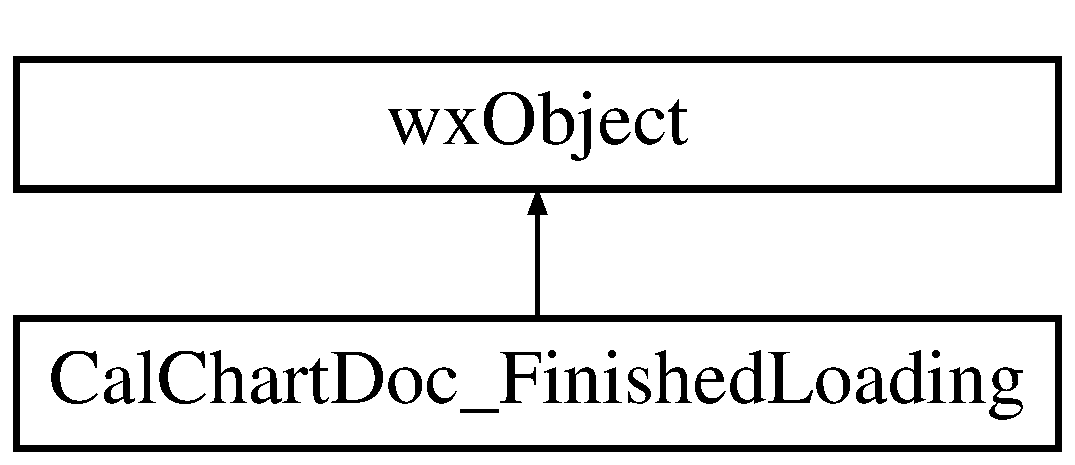
\includegraphics[height=2.000000cm]{a00021}
\end{center}
\end{figure}


The documentation for this class was generated from the following file\-:\begin{DoxyCompactItemize}
\item 
src/\hyperlink{a00181}{calchartdoc.\-h}\end{DoxyCompactItemize}

\hypertarget{a00022}{\section{Cal\-Chart\-Doc\-\_\-\-Flush\-All\-Views Class Reference}
\label{a00022}\index{Cal\-Chart\-Doc\-\_\-\-Flush\-All\-Views@{Cal\-Chart\-Doc\-\_\-\-Flush\-All\-Views}}
}


The \hyperlink{a00023}{Cal\-Chart\-Doc\-\_\-modified} class is used for indicating to views that they should save any text.  




{\ttfamily \#include $<$calchartdoc.\-h$>$}

Inheritance diagram for Cal\-Chart\-Doc\-\_\-\-Flush\-All\-Views\-:\begin{figure}[H]
\begin{center}
\leavevmode
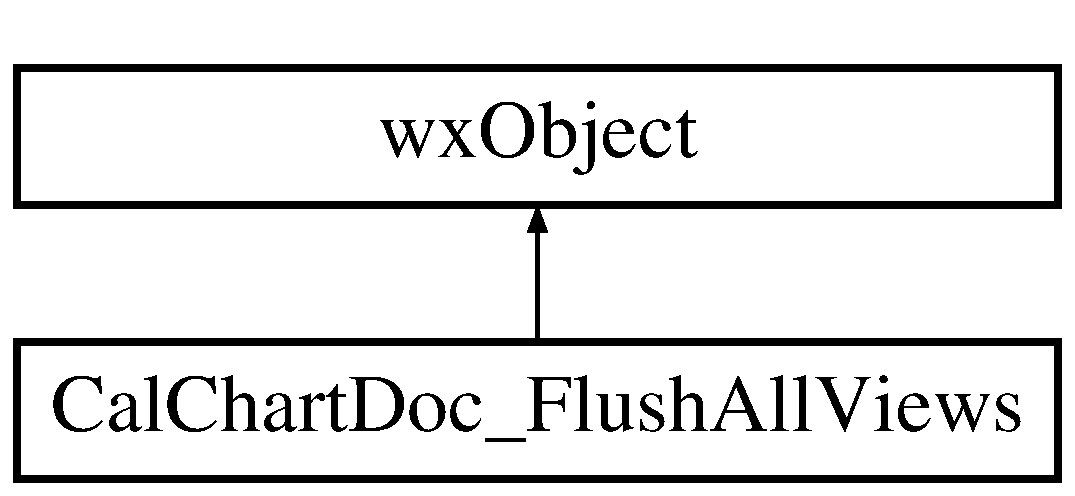
\includegraphics[height=2.000000cm]{a00022}
\end{center}
\end{figure}


\subsection{Detailed Description}
The \hyperlink{a00023}{Cal\-Chart\-Doc\-\_\-modified} class is used for indicating to views that they should save any text. 

The documentation for this class was generated from the following file\-:\begin{DoxyCompactItemize}
\item 
src/\hyperlink{a00181}{calchartdoc.\-h}\end{DoxyCompactItemize}

\hypertarget{a00023}{\section{Cal\-Chart\-Doc\-\_\-modified Class Reference}
\label{a00023}\index{Cal\-Chart\-Doc\-\_\-modified@{Cal\-Chart\-Doc\-\_\-modified}}
}


The \hyperlink{a00023}{Cal\-Chart\-Doc\-\_\-modified} class is used for indicating to views that the doc has been modified some views behave differently if the show has been modified.  




{\ttfamily \#include $<$calchartdoc.\-h$>$}

Inheritance diagram for Cal\-Chart\-Doc\-\_\-modified\-:\begin{figure}[H]
\begin{center}
\leavevmode
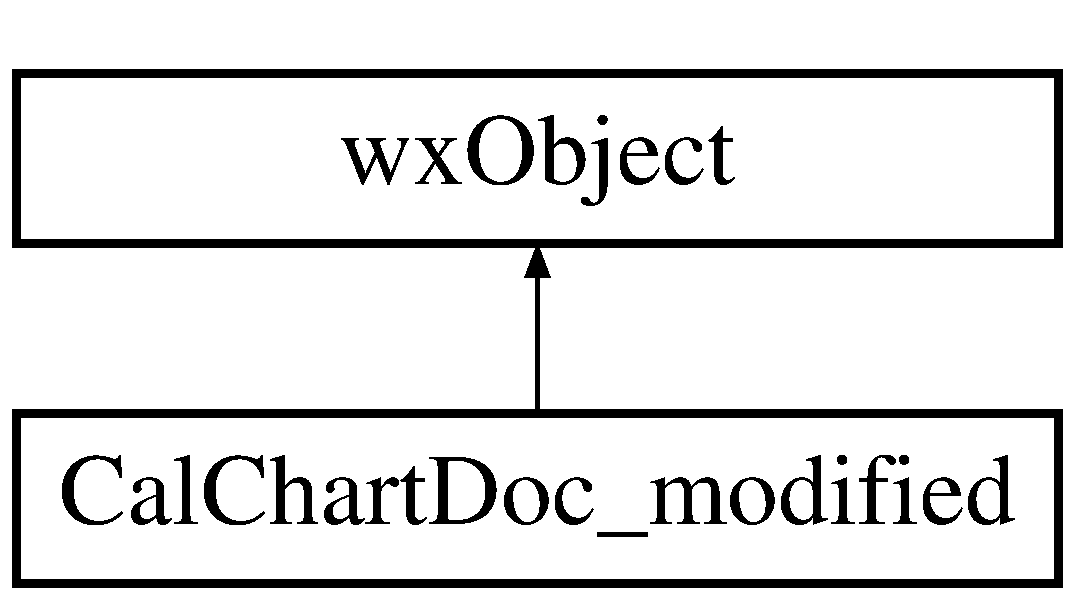
\includegraphics[height=2.000000cm]{a00023}
\end{center}
\end{figure}


\subsection{Detailed Description}
The \hyperlink{a00023}{Cal\-Chart\-Doc\-\_\-modified} class is used for indicating to views that the doc has been modified some views behave differently if the show has been modified. 

The documentation for this class was generated from the following file\-:\begin{DoxyCompactItemize}
\item 
src/\hyperlink{a00181}{calchartdoc.\-h}\end{DoxyCompactItemize}

\hypertarget{a00024}{\section{Cal\-Chart\-Doc\-\_\-setup Class Reference}
\label{a00024}\index{Cal\-Chart\-Doc\-\_\-setup@{Cal\-Chart\-Doc\-\_\-setup}}
}


{\ttfamily \#include $<$calchartdoc.\-h$>$}

Inheritance diagram for Cal\-Chart\-Doc\-\_\-setup\-:\begin{figure}[H]
\begin{center}
\leavevmode
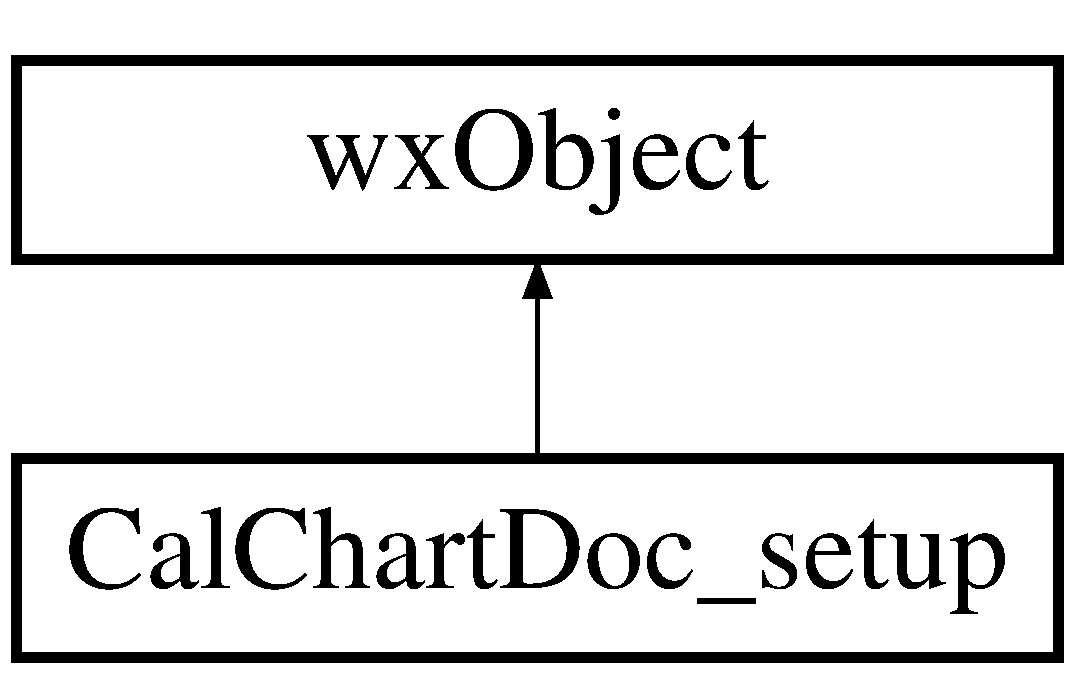
\includegraphics[height=2.000000cm]{a00024}
\end{center}
\end{figure}


The documentation for this class was generated from the following file\-:\begin{DoxyCompactItemize}
\item 
src/\hyperlink{a00181}{calchartdoc.\-h}\end{DoxyCompactItemize}

\hypertarget{a00025}{\section{Cal\-Chart\-Preferences Class Reference}
\label{a00025}\index{Cal\-Chart\-Preferences@{Cal\-Chart\-Preferences}}
}


{\ttfamily \#include $<$cc\-\_\-preferences\-\_\-ui.\-h$>$}

Inheritance diagram for Cal\-Chart\-Preferences\-:\begin{figure}[H]
\begin{center}
\leavevmode
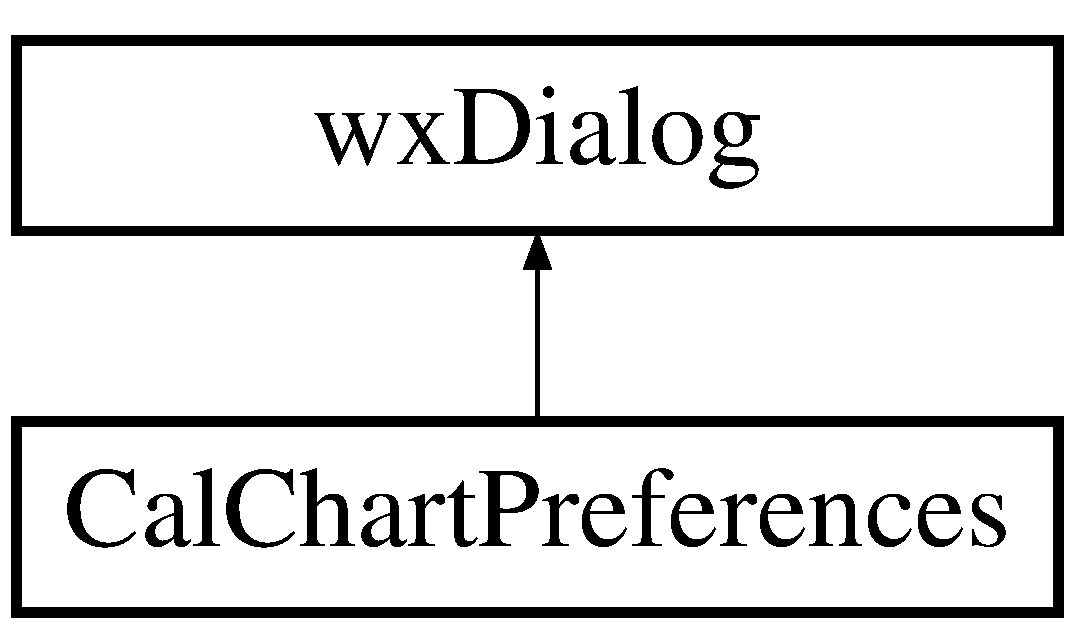
\includegraphics[height=2.000000cm]{a00025}
\end{center}
\end{figure}
\subsection*{Public Member Functions}
\begin{DoxyCompactItemize}
\item 
\hyperlink{a00025_a291efd287971e243c8735e04635ff74e}{Cal\-Chart\-Preferences} ()
\item 
\hyperlink{a00025_aa6229a327e8d66093267e8ce51293251}{Cal\-Chart\-Preferences} (wx\-Window $\ast$parent, wx\-Window\-I\-D id=wx\-I\-D\-\_\-\-A\-N\-Y, const wx\-String \&caption=wx\-T(\char`\"{}Cal\-Chart Preferences\char`\"{}), const wx\-Point \&pos=wx\-Default\-Position, const wx\-Size \&size=wx\-Default\-Size, long style=wx\-C\-A\-P\-T\-I\-O\-N$\vert$wx\-R\-E\-S\-I\-Z\-E\-\_\-\-B\-O\-R\-D\-E\-R$\vert$wx\-S\-Y\-S\-T\-E\-M\-\_\-\-M\-E\-N\-U)
\item 
\hyperlink{a00025_a2ac7dba36299d96c86e28f00d6dfac8b}{$\sim$\-Cal\-Chart\-Preferences} ()
\item 
void \hyperlink{a00025_aa093e353055f019c450ea79e7dc2c341}{Init} ()
\item 
bool \hyperlink{a00025_a95045856ad97ccd9bdd6121bbfe431d7}{Create} (wx\-Window $\ast$parent, wx\-Window\-I\-D id=wx\-I\-D\-\_\-\-A\-N\-Y, const wx\-String \&caption=wx\-T(\char`\"{}Cal\-Chart Preferences\char`\"{}), const wx\-Point \&pos=wx\-Default\-Position, const wx\-Size \&size=wx\-Default\-Size, long style=wx\-C\-A\-P\-T\-I\-O\-N$\vert$wx\-R\-E\-S\-I\-Z\-E\-\_\-\-B\-O\-R\-D\-E\-R$\vert$wx\-S\-Y\-S\-T\-E\-M\-\_\-\-M\-E\-N\-U)
\item 
void \hyperlink{a00025_ad51bb595a0f8e50375a9fd6e3be251c4}{Create\-Controls} ()
\item 
bool \hyperlink{a00025_acdce6207ef8c3d2523c5a947be8b57ca}{Transfer\-Data\-To\-Window} ()
\item 
bool \hyperlink{a00025_a7403ccca7f36bdbd8a7d1d3067d9a5a7}{Transfer\-Data\-From\-Window} ()
\end{DoxyCompactItemize}
\subsection*{Private Member Functions}
\begin{DoxyCompactItemize}
\item 
void \hyperlink{a00025_aa21276d4de4b8770aee283bb2fe7652c}{On\-Cmd\-Reset\-All} (wx\-Command\-Event \&)
\end{DoxyCompactItemize}
\subsection*{Private Attributes}
\begin{DoxyCompactItemize}
\item 
wx\-Notebook $\ast$ \hyperlink{a00025_a27535ea08c2c16709650a92e74ced8c3}{m\-Notebook}
\end{DoxyCompactItemize}


\subsection{Constructor \& Destructor Documentation}
\hypertarget{a00025_a291efd287971e243c8735e04635ff74e}{\index{Cal\-Chart\-Preferences@{Cal\-Chart\-Preferences}!Cal\-Chart\-Preferences@{Cal\-Chart\-Preferences}}
\index{Cal\-Chart\-Preferences@{Cal\-Chart\-Preferences}!CalChartPreferences@{Cal\-Chart\-Preferences}}
\subsubsection[{Cal\-Chart\-Preferences}]{\setlength{\rightskip}{0pt plus 5cm}Cal\-Chart\-Preferences\-::\-Cal\-Chart\-Preferences (
\begin{DoxyParamCaption}
{}
\end{DoxyParamCaption}
)}}\label{a00025_a291efd287971e243c8735e04635ff74e}
\hypertarget{a00025_aa6229a327e8d66093267e8ce51293251}{\index{Cal\-Chart\-Preferences@{Cal\-Chart\-Preferences}!Cal\-Chart\-Preferences@{Cal\-Chart\-Preferences}}
\index{Cal\-Chart\-Preferences@{Cal\-Chart\-Preferences}!CalChartPreferences@{Cal\-Chart\-Preferences}}
\subsubsection[{Cal\-Chart\-Preferences}]{\setlength{\rightskip}{0pt plus 5cm}Cal\-Chart\-Preferences\-::\-Cal\-Chart\-Preferences (
\begin{DoxyParamCaption}
\item[{wx\-Window $\ast$}]{parent, }
\item[{wx\-Window\-I\-D}]{id = {\ttfamily wxID\-\_\-ANY}, }
\item[{const wx\-String \&}]{caption = {\ttfamily wxT(\char`\"{}CalChart~Preferences\char`\"{})}, }
\item[{const wx\-Point \&}]{pos = {\ttfamily wxDefaultPosition}, }
\item[{const wx\-Size \&}]{size = {\ttfamily wxDefaultSize}, }
\item[{long}]{style = {\ttfamily wxCAPTION$\vert$wxRESIZE\-\_\-BORDER$\vert$wxSYSTEM\-\_\-MENU}}
\end{DoxyParamCaption}
)}}\label{a00025_aa6229a327e8d66093267e8ce51293251}
\hypertarget{a00025_a2ac7dba36299d96c86e28f00d6dfac8b}{\index{Cal\-Chart\-Preferences@{Cal\-Chart\-Preferences}!$\sim$\-Cal\-Chart\-Preferences@{$\sim$\-Cal\-Chart\-Preferences}}
\index{$\sim$\-Cal\-Chart\-Preferences@{$\sim$\-Cal\-Chart\-Preferences}!CalChartPreferences@{Cal\-Chart\-Preferences}}
\subsubsection[{$\sim$\-Cal\-Chart\-Preferences}]{\setlength{\rightskip}{0pt plus 5cm}Cal\-Chart\-Preferences\-::$\sim$\-Cal\-Chart\-Preferences (
\begin{DoxyParamCaption}
{}
\end{DoxyParamCaption}
)}}\label{a00025_a2ac7dba36299d96c86e28f00d6dfac8b}


\subsection{Member Function Documentation}
\hypertarget{a00025_a95045856ad97ccd9bdd6121bbfe431d7}{\index{Cal\-Chart\-Preferences@{Cal\-Chart\-Preferences}!Create@{Create}}
\index{Create@{Create}!CalChartPreferences@{Cal\-Chart\-Preferences}}
\subsubsection[{Create}]{\setlength{\rightskip}{0pt plus 5cm}bool Cal\-Chart\-Preferences\-::\-Create (
\begin{DoxyParamCaption}
\item[{wx\-Window $\ast$}]{parent, }
\item[{wx\-Window\-I\-D}]{id = {\ttfamily wxID\-\_\-ANY}, }
\item[{const wx\-String \&}]{caption = {\ttfamily wxT(\char`\"{}CalChart~Preferences\char`\"{})}, }
\item[{const wx\-Point \&}]{pos = {\ttfamily wxDefaultPosition}, }
\item[{const wx\-Size \&}]{size = {\ttfamily wxDefaultSize}, }
\item[{long}]{style = {\ttfamily wxCAPTION$\vert$wxRESIZE\-\_\-BORDER$\vert$wxSYSTEM\-\_\-MENU}}
\end{DoxyParamCaption}
)}}\label{a00025_a95045856ad97ccd9bdd6121bbfe431d7}
\hypertarget{a00025_ad51bb595a0f8e50375a9fd6e3be251c4}{\index{Cal\-Chart\-Preferences@{Cal\-Chart\-Preferences}!Create\-Controls@{Create\-Controls}}
\index{Create\-Controls@{Create\-Controls}!CalChartPreferences@{Cal\-Chart\-Preferences}}
\subsubsection[{Create\-Controls}]{\setlength{\rightskip}{0pt plus 5cm}void Cal\-Chart\-Preferences\-::\-Create\-Controls (
\begin{DoxyParamCaption}
{}
\end{DoxyParamCaption}
)}}\label{a00025_ad51bb595a0f8e50375a9fd6e3be251c4}
\hypertarget{a00025_aa093e353055f019c450ea79e7dc2c341}{\index{Cal\-Chart\-Preferences@{Cal\-Chart\-Preferences}!Init@{Init}}
\index{Init@{Init}!CalChartPreferences@{Cal\-Chart\-Preferences}}
\subsubsection[{Init}]{\setlength{\rightskip}{0pt plus 5cm}void Cal\-Chart\-Preferences\-::\-Init (
\begin{DoxyParamCaption}
{}
\end{DoxyParamCaption}
)}}\label{a00025_aa093e353055f019c450ea79e7dc2c341}
\hypertarget{a00025_aa21276d4de4b8770aee283bb2fe7652c}{\index{Cal\-Chart\-Preferences@{Cal\-Chart\-Preferences}!On\-Cmd\-Reset\-All@{On\-Cmd\-Reset\-All}}
\index{On\-Cmd\-Reset\-All@{On\-Cmd\-Reset\-All}!CalChartPreferences@{Cal\-Chart\-Preferences}}
\subsubsection[{On\-Cmd\-Reset\-All}]{\setlength{\rightskip}{0pt plus 5cm}void Cal\-Chart\-Preferences\-::\-On\-Cmd\-Reset\-All (
\begin{DoxyParamCaption}
\item[{wx\-Command\-Event \&}]{}
\end{DoxyParamCaption}
)\hspace{0.3cm}{\ttfamily [private]}}}\label{a00025_aa21276d4de4b8770aee283bb2fe7652c}
\hypertarget{a00025_a7403ccca7f36bdbd8a7d1d3067d9a5a7}{\index{Cal\-Chart\-Preferences@{Cal\-Chart\-Preferences}!Transfer\-Data\-From\-Window@{Transfer\-Data\-From\-Window}}
\index{Transfer\-Data\-From\-Window@{Transfer\-Data\-From\-Window}!CalChartPreferences@{Cal\-Chart\-Preferences}}
\subsubsection[{Transfer\-Data\-From\-Window}]{\setlength{\rightskip}{0pt plus 5cm}bool Cal\-Chart\-Preferences\-::\-Transfer\-Data\-From\-Window (
\begin{DoxyParamCaption}
{}
\end{DoxyParamCaption}
)}}\label{a00025_a7403ccca7f36bdbd8a7d1d3067d9a5a7}
\hypertarget{a00025_acdce6207ef8c3d2523c5a947be8b57ca}{\index{Cal\-Chart\-Preferences@{Cal\-Chart\-Preferences}!Transfer\-Data\-To\-Window@{Transfer\-Data\-To\-Window}}
\index{Transfer\-Data\-To\-Window@{Transfer\-Data\-To\-Window}!CalChartPreferences@{Cal\-Chart\-Preferences}}
\subsubsection[{Transfer\-Data\-To\-Window}]{\setlength{\rightskip}{0pt plus 5cm}bool Cal\-Chart\-Preferences\-::\-Transfer\-Data\-To\-Window (
\begin{DoxyParamCaption}
{}
\end{DoxyParamCaption}
)}}\label{a00025_acdce6207ef8c3d2523c5a947be8b57ca}


\subsection{Member Data Documentation}
\hypertarget{a00025_a27535ea08c2c16709650a92e74ced8c3}{\index{Cal\-Chart\-Preferences@{Cal\-Chart\-Preferences}!m\-Notebook@{m\-Notebook}}
\index{m\-Notebook@{m\-Notebook}!CalChartPreferences@{Cal\-Chart\-Preferences}}
\subsubsection[{m\-Notebook}]{\setlength{\rightskip}{0pt plus 5cm}wx\-Notebook$\ast$ Cal\-Chart\-Preferences\-::m\-Notebook\hspace{0.3cm}{\ttfamily [private]}}}\label{a00025_a27535ea08c2c16709650a92e74ced8c3}


The documentation for this class was generated from the following files\-:\begin{DoxyCompactItemize}
\item 
src/\hyperlink{a00188}{cc\-\_\-preferences\-\_\-ui.\-h}\item 
src/\hyperlink{a00187}{cc\-\_\-preferences\-\_\-ui.\-cpp}\end{DoxyCompactItemize}

\hypertarget{a00026}{\section{Background\-Image\-:\-:Calculate\-Scale\-And\-Move Class Reference}
\label{a00026}\index{Background\-Image\-::\-Calculate\-Scale\-And\-Move@{Background\-Image\-::\-Calculate\-Scale\-And\-Move}}
}
\subsection*{Public Member Functions}
\begin{DoxyCompactItemize}
\item 
\hyperlink{a00026_acdc1b3f9e19c9c7df4ab4c8b5ef3ba83}{Calculate\-Scale\-And\-Move} (const wx\-Point \&start\-Click, wx\-Coord x, wx\-Coord y, long width, long height, \hyperlink{a00017_a3927289a3b88bbf9320c2dfe3271c1ae}{e\-Background\-Adjust\-Type} adjust\-Type)
\item 
void \hyperlink{a00026_a5d5b2066e9e55332cef810e5220e7171}{operator()} (long x, long y, wx\-Coord \&top\-X, wx\-Coord \&top\-Y, wx\-Coord \&width, wx\-Coord \&height)
\end{DoxyCompactItemize}
\subsection*{Public Attributes}
\begin{DoxyCompactItemize}
\item 
wx\-Point \hyperlink{a00026_abfc1d7e1dedf3cd3849b801b5359fd6f}{m\-Start\-Click}
\item 
wx\-Coord \hyperlink{a00026_a6cb63ace64accd5ac8c3a829a3cb64bc}{m\-Left}
\item 
wx\-Coord \hyperlink{a00026_a906cd5b5471e32132eb3ae4e7662f641}{m\-Top}
\item 
wx\-Coord \hyperlink{a00026_a5559ceef31f1942d05452e2f6f17cfb8}{m\-Right}
\item 
wx\-Coord \hyperlink{a00026_a694323b8aa12e93f816074d8e15bf665}{m\-Bottom}
\item 
float \hyperlink{a00026_abd99704a6e867545436f7c16e483d585}{m\-Aspect\-Ratio}
\item 
\hyperlink{a00017_a3927289a3b88bbf9320c2dfe3271c1ae}{e\-Background\-Adjust\-Type} \hyperlink{a00026_a65984a6ed965e2c524a76831d08ac3bd}{m\-Adjust\-Type}
\end{DoxyCompactItemize}


\subsection{Constructor \& Destructor Documentation}
\hypertarget{a00026_acdc1b3f9e19c9c7df4ab4c8b5ef3ba83}{\index{Background\-Image\-::\-Calculate\-Scale\-And\-Move@{Background\-Image\-::\-Calculate\-Scale\-And\-Move}!Calculate\-Scale\-And\-Move@{Calculate\-Scale\-And\-Move}}
\index{Calculate\-Scale\-And\-Move@{Calculate\-Scale\-And\-Move}!BackgroundImage::CalculateScaleAndMove@{Background\-Image\-::\-Calculate\-Scale\-And\-Move}}
\subsubsection[{Calculate\-Scale\-And\-Move}]{\setlength{\rightskip}{0pt plus 5cm}Background\-Image\-::\-Calculate\-Scale\-And\-Move\-::\-Calculate\-Scale\-And\-Move (
\begin{DoxyParamCaption}
\item[{const wx\-Point \&}]{start\-Click, }
\item[{wx\-Coord}]{x, }
\item[{wx\-Coord}]{y, }
\item[{long}]{width, }
\item[{long}]{height, }
\item[{{\bf e\-Background\-Adjust\-Type}}]{adjust\-Type}
\end{DoxyParamCaption}
)}}\label{a00026_acdc1b3f9e19c9c7df4ab4c8b5ef3ba83}


\subsection{Member Function Documentation}
\hypertarget{a00026_a5d5b2066e9e55332cef810e5220e7171}{\index{Background\-Image\-::\-Calculate\-Scale\-And\-Move@{Background\-Image\-::\-Calculate\-Scale\-And\-Move}!operator()@{operator()}}
\index{operator()@{operator()}!BackgroundImage::CalculateScaleAndMove@{Background\-Image\-::\-Calculate\-Scale\-And\-Move}}
\subsubsection[{operator()}]{\setlength{\rightskip}{0pt plus 5cm}void Background\-Image\-::\-Calculate\-Scale\-And\-Move\-::operator() (
\begin{DoxyParamCaption}
\item[{long}]{x, }
\item[{long}]{y, }
\item[{wx\-Coord \&}]{top\-X, }
\item[{wx\-Coord \&}]{top\-Y, }
\item[{wx\-Coord \&}]{width, }
\item[{wx\-Coord \&}]{height}
\end{DoxyParamCaption}
)}}\label{a00026_a5d5b2066e9e55332cef810e5220e7171}


\subsection{Member Data Documentation}
\hypertarget{a00026_a65984a6ed965e2c524a76831d08ac3bd}{\index{Background\-Image\-::\-Calculate\-Scale\-And\-Move@{Background\-Image\-::\-Calculate\-Scale\-And\-Move}!m\-Adjust\-Type@{m\-Adjust\-Type}}
\index{m\-Adjust\-Type@{m\-Adjust\-Type}!BackgroundImage::CalculateScaleAndMove@{Background\-Image\-::\-Calculate\-Scale\-And\-Move}}
\subsubsection[{m\-Adjust\-Type}]{\setlength{\rightskip}{0pt plus 5cm}{\bf e\-Background\-Adjust\-Type} Background\-Image\-::\-Calculate\-Scale\-And\-Move\-::m\-Adjust\-Type}}\label{a00026_a65984a6ed965e2c524a76831d08ac3bd}
\hypertarget{a00026_abd99704a6e867545436f7c16e483d585}{\index{Background\-Image\-::\-Calculate\-Scale\-And\-Move@{Background\-Image\-::\-Calculate\-Scale\-And\-Move}!m\-Aspect\-Ratio@{m\-Aspect\-Ratio}}
\index{m\-Aspect\-Ratio@{m\-Aspect\-Ratio}!BackgroundImage::CalculateScaleAndMove@{Background\-Image\-::\-Calculate\-Scale\-And\-Move}}
\subsubsection[{m\-Aspect\-Ratio}]{\setlength{\rightskip}{0pt plus 5cm}float Background\-Image\-::\-Calculate\-Scale\-And\-Move\-::m\-Aspect\-Ratio}}\label{a00026_abd99704a6e867545436f7c16e483d585}
\hypertarget{a00026_a694323b8aa12e93f816074d8e15bf665}{\index{Background\-Image\-::\-Calculate\-Scale\-And\-Move@{Background\-Image\-::\-Calculate\-Scale\-And\-Move}!m\-Bottom@{m\-Bottom}}
\index{m\-Bottom@{m\-Bottom}!BackgroundImage::CalculateScaleAndMove@{Background\-Image\-::\-Calculate\-Scale\-And\-Move}}
\subsubsection[{m\-Bottom}]{\setlength{\rightskip}{0pt plus 5cm}wx\-Coord Background\-Image\-::\-Calculate\-Scale\-And\-Move\-::m\-Bottom}}\label{a00026_a694323b8aa12e93f816074d8e15bf665}
\hypertarget{a00026_a6cb63ace64accd5ac8c3a829a3cb64bc}{\index{Background\-Image\-::\-Calculate\-Scale\-And\-Move@{Background\-Image\-::\-Calculate\-Scale\-And\-Move}!m\-Left@{m\-Left}}
\index{m\-Left@{m\-Left}!BackgroundImage::CalculateScaleAndMove@{Background\-Image\-::\-Calculate\-Scale\-And\-Move}}
\subsubsection[{m\-Left}]{\setlength{\rightskip}{0pt plus 5cm}wx\-Coord Background\-Image\-::\-Calculate\-Scale\-And\-Move\-::m\-Left}}\label{a00026_a6cb63ace64accd5ac8c3a829a3cb64bc}
\hypertarget{a00026_a5559ceef31f1942d05452e2f6f17cfb8}{\index{Background\-Image\-::\-Calculate\-Scale\-And\-Move@{Background\-Image\-::\-Calculate\-Scale\-And\-Move}!m\-Right@{m\-Right}}
\index{m\-Right@{m\-Right}!BackgroundImage::CalculateScaleAndMove@{Background\-Image\-::\-Calculate\-Scale\-And\-Move}}
\subsubsection[{m\-Right}]{\setlength{\rightskip}{0pt plus 5cm}wx\-Coord Background\-Image\-::\-Calculate\-Scale\-And\-Move\-::m\-Right}}\label{a00026_a5559ceef31f1942d05452e2f6f17cfb8}
\hypertarget{a00026_abfc1d7e1dedf3cd3849b801b5359fd6f}{\index{Background\-Image\-::\-Calculate\-Scale\-And\-Move@{Background\-Image\-::\-Calculate\-Scale\-And\-Move}!m\-Start\-Click@{m\-Start\-Click}}
\index{m\-Start\-Click@{m\-Start\-Click}!BackgroundImage::CalculateScaleAndMove@{Background\-Image\-::\-Calculate\-Scale\-And\-Move}}
\subsubsection[{m\-Start\-Click}]{\setlength{\rightskip}{0pt plus 5cm}wx\-Point Background\-Image\-::\-Calculate\-Scale\-And\-Move\-::m\-Start\-Click}}\label{a00026_abfc1d7e1dedf3cd3849b801b5359fd6f}
\hypertarget{a00026_a906cd5b5471e32132eb3ae4e7662f641}{\index{Background\-Image\-::\-Calculate\-Scale\-And\-Move@{Background\-Image\-::\-Calculate\-Scale\-And\-Move}!m\-Top@{m\-Top}}
\index{m\-Top@{m\-Top}!BackgroundImage::CalculateScaleAndMove@{Background\-Image\-::\-Calculate\-Scale\-And\-Move}}
\subsubsection[{m\-Top}]{\setlength{\rightskip}{0pt plus 5cm}wx\-Coord Background\-Image\-::\-Calculate\-Scale\-And\-Move\-::m\-Top}}\label{a00026_a906cd5b5471e32132eb3ae4e7662f641}


The documentation for this class was generated from the following files\-:\begin{DoxyCompactItemize}
\item 
src/\hyperlink{a00175}{background\-\_\-image.\-h}\item 
src/\hyperlink{a00174}{background\-\_\-image.\-cpp}\end{DoxyCompactItemize}

\hypertarget{a00027}{\section{C\-C\-\_\-continuity Class Reference}
\label{a00027}\index{C\-C\-\_\-continuity@{C\-C\-\_\-continuity}}
}


{\ttfamily \#include $<$cc\-\_\-continuity.\-h$>$}

\subsection*{Public Member Functions}
\begin{DoxyCompactItemize}
\item 
\hyperlink{a00027_afa0aca56563b833b298b667a76d9315b}{C\-C\-\_\-continuity} ()
\item 
\hyperlink{a00027_a8576a67b4911b90fd5afdba1758a9b0f}{$\sim$\-C\-C\-\_\-continuity} ()
\item 
void \hyperlink{a00027_a78c9ab90849f26ee2e5d83de10fc2a0c}{Set\-Text} (const std\-::string \&s)
\item 
void \hyperlink{a00027_a33de69f358d44142b9a62951f0d6c4bb}{Append\-Text} (const std\-::string \&s)
\item 
const std\-::string \& \hyperlink{a00027_a9ce5e3a542e765aa259cf57d374fa46b}{Get\-Text} () const 
\end{DoxyCompactItemize}
\subsection*{Private Attributes}
\begin{DoxyCompactItemize}
\item 
std\-::string \hyperlink{a00027_a7b5d41e8b0aa73c2d8423a7bd27b27fa}{text}
\end{DoxyCompactItemize}
\subsection*{Friends}
\begin{DoxyCompactItemize}
\item 
bool \hyperlink{a00027_ac961436b35c4fb9e497123dcea1a21e6}{Check\-\_\-\-C\-C\-\_\-continuity} (const \hyperlink{a00027}{C\-C\-\_\-continuity} \&, const struct \hyperlink{a00028}{C\-C\-\_\-continuity\-\_\-values} \&)
\item 
void \hyperlink{a00027_a8daadaacfcc6d54a48f7853fe864bc46}{C\-C\-\_\-continuity\-\_\-\-Unit\-Tests} ()
\end{DoxyCompactItemize}


\subsection{Constructor \& Destructor Documentation}
\hypertarget{a00027_afa0aca56563b833b298b667a76d9315b}{\index{C\-C\-\_\-continuity@{C\-C\-\_\-continuity}!C\-C\-\_\-continuity@{C\-C\-\_\-continuity}}
\index{C\-C\-\_\-continuity@{C\-C\-\_\-continuity}!CC_continuity@{C\-C\-\_\-continuity}}
\subsubsection[{C\-C\-\_\-continuity}]{\setlength{\rightskip}{0pt plus 5cm}C\-C\-\_\-continuity\-::\-C\-C\-\_\-continuity (
\begin{DoxyParamCaption}
{}
\end{DoxyParamCaption}
)}}\label{a00027_afa0aca56563b833b298b667a76d9315b}
\hypertarget{a00027_a8576a67b4911b90fd5afdba1758a9b0f}{\index{C\-C\-\_\-continuity@{C\-C\-\_\-continuity}!$\sim$\-C\-C\-\_\-continuity@{$\sim$\-C\-C\-\_\-continuity}}
\index{$\sim$\-C\-C\-\_\-continuity@{$\sim$\-C\-C\-\_\-continuity}!CC_continuity@{C\-C\-\_\-continuity}}
\subsubsection[{$\sim$\-C\-C\-\_\-continuity}]{\setlength{\rightskip}{0pt plus 5cm}C\-C\-\_\-continuity\-::$\sim$\-C\-C\-\_\-continuity (
\begin{DoxyParamCaption}
{}
\end{DoxyParamCaption}
)}}\label{a00027_a8576a67b4911b90fd5afdba1758a9b0f}


\subsection{Member Function Documentation}
\hypertarget{a00027_a33de69f358d44142b9a62951f0d6c4bb}{\index{C\-C\-\_\-continuity@{C\-C\-\_\-continuity}!Append\-Text@{Append\-Text}}
\index{Append\-Text@{Append\-Text}!CC_continuity@{C\-C\-\_\-continuity}}
\subsubsection[{Append\-Text}]{\setlength{\rightskip}{0pt plus 5cm}void C\-C\-\_\-continuity\-::\-Append\-Text (
\begin{DoxyParamCaption}
\item[{const std\-::string \&}]{s}
\end{DoxyParamCaption}
)}}\label{a00027_a33de69f358d44142b9a62951f0d6c4bb}
\hypertarget{a00027_a9ce5e3a542e765aa259cf57d374fa46b}{\index{C\-C\-\_\-continuity@{C\-C\-\_\-continuity}!Get\-Text@{Get\-Text}}
\index{Get\-Text@{Get\-Text}!CC_continuity@{C\-C\-\_\-continuity}}
\subsubsection[{Get\-Text}]{\setlength{\rightskip}{0pt plus 5cm}const string \& C\-C\-\_\-continuity\-::\-Get\-Text (
\begin{DoxyParamCaption}
{}
\end{DoxyParamCaption}
) const}}\label{a00027_a9ce5e3a542e765aa259cf57d374fa46b}
\hypertarget{a00027_a78c9ab90849f26ee2e5d83de10fc2a0c}{\index{C\-C\-\_\-continuity@{C\-C\-\_\-continuity}!Set\-Text@{Set\-Text}}
\index{Set\-Text@{Set\-Text}!CC_continuity@{C\-C\-\_\-continuity}}
\subsubsection[{Set\-Text}]{\setlength{\rightskip}{0pt plus 5cm}void C\-C\-\_\-continuity\-::\-Set\-Text (
\begin{DoxyParamCaption}
\item[{const std\-::string \&}]{s}
\end{DoxyParamCaption}
)}}\label{a00027_a78c9ab90849f26ee2e5d83de10fc2a0c}


\subsection{Friends And Related Function Documentation}
\hypertarget{a00027_a8daadaacfcc6d54a48f7853fe864bc46}{\index{C\-C\-\_\-continuity@{C\-C\-\_\-continuity}!C\-C\-\_\-continuity\-\_\-\-Unit\-Tests@{C\-C\-\_\-continuity\-\_\-\-Unit\-Tests}}
\index{C\-C\-\_\-continuity\-\_\-\-Unit\-Tests@{C\-C\-\_\-continuity\-\_\-\-Unit\-Tests}!CC_continuity@{C\-C\-\_\-continuity}}
\subsubsection[{C\-C\-\_\-continuity\-\_\-\-Unit\-Tests}]{\setlength{\rightskip}{0pt plus 5cm}void C\-C\-\_\-continuity\-\_\-\-Unit\-Tests (
\begin{DoxyParamCaption}
{}
\end{DoxyParamCaption}
)\hspace{0.3cm}{\ttfamily [friend]}}}\label{a00027_a8daadaacfcc6d54a48f7853fe864bc46}
\hypertarget{a00027_ac961436b35c4fb9e497123dcea1a21e6}{\index{C\-C\-\_\-continuity@{C\-C\-\_\-continuity}!Check\-\_\-\-C\-C\-\_\-continuity@{Check\-\_\-\-C\-C\-\_\-continuity}}
\index{Check\-\_\-\-C\-C\-\_\-continuity@{Check\-\_\-\-C\-C\-\_\-continuity}!CC_continuity@{C\-C\-\_\-continuity}}
\subsubsection[{Check\-\_\-\-C\-C\-\_\-continuity}]{\setlength{\rightskip}{0pt plus 5cm}bool Check\-\_\-\-C\-C\-\_\-continuity (
\begin{DoxyParamCaption}
\item[{const {\bf C\-C\-\_\-continuity} \&}]{, }
\item[{const struct {\bf C\-C\-\_\-continuity\-\_\-values} \&}]{}
\end{DoxyParamCaption}
)\hspace{0.3cm}{\ttfamily [friend]}}}\label{a00027_ac961436b35c4fb9e497123dcea1a21e6}


\subsection{Member Data Documentation}
\hypertarget{a00027_a7b5d41e8b0aa73c2d8423a7bd27b27fa}{\index{C\-C\-\_\-continuity@{C\-C\-\_\-continuity}!text@{text}}
\index{text@{text}!CC_continuity@{C\-C\-\_\-continuity}}
\subsubsection[{text}]{\setlength{\rightskip}{0pt plus 5cm}std\-::string C\-C\-\_\-continuity\-::text\hspace{0.3cm}{\ttfamily [private]}}}\label{a00027_a7b5d41e8b0aa73c2d8423a7bd27b27fa}


The documentation for this class was generated from the following files\-:\begin{DoxyCompactItemize}
\item 
src/core/\hyperlink{a00202}{cc\-\_\-continuity.\-h}\item 
src/core/\hyperlink{a00201}{cc\-\_\-continuity.\-cpp}\end{DoxyCompactItemize}

\hypertarget{a00028}{\section{C\-C\-\_\-continuity\-\_\-values Struct Reference}
\label{a00028}\index{C\-C\-\_\-continuity\-\_\-values@{C\-C\-\_\-continuity\-\_\-values}}
}
\subsection*{Public Attributes}
\begin{DoxyCompactItemize}
\item 
string \hyperlink{a00028_ac2607e51859f3ceb24f7fd49d0fe2516}{text}
\item 
string \hyperlink{a00028_a51f4e7859eb92c164044d35642139210}{Get\-Text}
\end{DoxyCompactItemize}


\subsection{Member Data Documentation}
\hypertarget{a00028_a51f4e7859eb92c164044d35642139210}{\index{C\-C\-\_\-continuity\-\_\-values@{C\-C\-\_\-continuity\-\_\-values}!Get\-Text@{Get\-Text}}
\index{Get\-Text@{Get\-Text}!CC_continuity_values@{C\-C\-\_\-continuity\-\_\-values}}
\subsubsection[{Get\-Text}]{\setlength{\rightskip}{0pt plus 5cm}string C\-C\-\_\-continuity\-\_\-values\-::\-Get\-Text}}\label{a00028_a51f4e7859eb92c164044d35642139210}
\hypertarget{a00028_ac2607e51859f3ceb24f7fd49d0fe2516}{\index{C\-C\-\_\-continuity\-\_\-values@{C\-C\-\_\-continuity\-\_\-values}!text@{text}}
\index{text@{text}!CC_continuity_values@{C\-C\-\_\-continuity\-\_\-values}}
\subsubsection[{text}]{\setlength{\rightskip}{0pt plus 5cm}string C\-C\-\_\-continuity\-\_\-values\-::text}}\label{a00028_ac2607e51859f3ceb24f7fd49d0fe2516}


The documentation for this struct was generated from the following file\-:\begin{DoxyCompactItemize}
\item 
src/core/\hyperlink{a00201}{cc\-\_\-continuity.\-cpp}\end{DoxyCompactItemize}

\hypertarget{a00029}{\section{C\-C\-\_\-coord Class Reference}
\label{a00029}\index{C\-C\-\_\-coord@{C\-C\-\_\-coord}}
}


A two dimensional vector that can be used to represent a coordinate in Cal\-Chart.  




{\ttfamily \#include $<$cc\-\_\-coord.\-h$>$}

\subsection*{Public Member Functions}
\begin{DoxyCompactItemize}
\item 
\hyperlink{a00029_a69194d9f67638d9a89c9288924b0f9e2}{C\-C\-\_\-coord} (\hyperlink{a00216_acd9dae57b712df0e2d3588c0c4798c11}{Coord} xval=0, \hyperlink{a00216_acd9dae57b712df0e2d3588c0c4798c11}{Coord} yval=0)
\begin{DoxyCompactList}\small\item\em Constructs a coordinate (or vector) with the specified coordinates. \end{DoxyCompactList}\item 
float \hyperlink{a00029_ad64566e6ad9d6515d0393f6e886f1f6e}{Magnitude} () const 
\begin{DoxyCompactList}\small\item\em Returns the magnitude of the vector represented by this object. \end{DoxyCompactList}\item 
float \hyperlink{a00029_ac197fb1a92a5f468d91c19b0e28576a0}{D\-M\-\_\-\-Magnitude} () const 
\begin{DoxyCompactList}\small\item\em Returns the magnitude of \hyperlink{a00029}{C\-C\-\_\-coord}, as defined by the \hyperlink{a00029_ad64566e6ad9d6515d0393f6e886f1f6e}{Magnitude()} method, I\-F the vector represented by \hyperlink{a00029}{C\-C\-\_\-coord} does not make a 45 degree angle with the x or y axis (which occurs when the x component is either equal to the y component or its negative). \end{DoxyCompactList}\item 
float \hyperlink{a00029_a508c84e70e6f919e7badc4ca72e27516}{Direction} () const 
\begin{DoxyCompactList}\small\item\em Returns the angle between the vector represented by this \hyperlink{a00029}{C\-C\-\_\-coord} and a vector pointing along the positive x direction; that is, the angle returned is the angle of the vector in standard position. \end{DoxyCompactList}\item 
float \hyperlink{a00029_add644be1d01386682dd8eb115b4af7b9}{Direction} (const \hyperlink{a00029}{C\-C\-\_\-coord} \&c) const 
\begin{DoxyCompactList}\small\item\em Returns the direction of the vector (from standard position) that starts at the point represented by this \hyperlink{a00029}{C\-C\-\_\-coord} and ends at the point represented by the parameter. \end{DoxyCompactList}\item 
bool \hyperlink{a00029_af4fff5071fce15aa9b316de2d7980f6e}{Collides} (const \hyperlink{a00029}{C\-C\-\_\-coord} \&c) const 
\begin{DoxyCompactList}\small\item\em Returns true if this \hyperlink{a00029}{C\-C\-\_\-coord} object is within one step of the one passed as a parameter (where one step is the standard unit of the x and y coordinates of a \hyperlink{a00029}{C\-C\-\_\-coord}); returns false otherwise. \end{DoxyCompactList}\item 
\hyperlink{a00029}{C\-C\-\_\-coord} \& \hyperlink{a00029_a61000324a3fe34fa9579fa43578b7ca3}{operator+=} (const \hyperlink{a00029}{C\-C\-\_\-coord} \&c)
\begin{DoxyCompactList}\small\item\em Performs vector addition. \end{DoxyCompactList}\item 
\hyperlink{a00029}{C\-C\-\_\-coord} \& \hyperlink{a00029_afa570bee9df745b6639fff9fc39a906f}{operator-\/=} (const \hyperlink{a00029}{C\-C\-\_\-coord} \&c)
\begin{DoxyCompactList}\small\item\em Performs vector subtraction. \end{DoxyCompactList}\item 
\hyperlink{a00029}{C\-C\-\_\-coord} \& \hyperlink{a00029_a7d719b060f44d62e846636f88535f692}{operator$\ast$=} (short s)
\begin{DoxyCompactList}\small\item\em Performs vector-\/scalar multiplication. \end{DoxyCompactList}\item 
\hyperlink{a00029}{C\-C\-\_\-coord} \& \hyperlink{a00029_a4d7b64280048bad9022cafaeecbb94db}{operator/=} (short s)
\begin{DoxyCompactList}\small\item\em Performs vector-\/scalar division. \end{DoxyCompactList}\end{DoxyCompactItemize}
\subsection*{Public Attributes}
\begin{DoxyCompactItemize}
\item 
\hyperlink{a00216_acd9dae57b712df0e2d3588c0c4798c11}{Coord} \hyperlink{a00029_a4000dc426fbaa84ee0949161e2c2a8ef}{x}
\begin{DoxyCompactList}\small\item\em The X component of the vector. \end{DoxyCompactList}\item 
\hyperlink{a00216_acd9dae57b712df0e2d3588c0c4798c11}{Coord} \hyperlink{a00029_affa708ad9c6f0aa792f8fd4a537a9c12}{y}
\begin{DoxyCompactList}\small\item\em The Y component of the vector. \end{DoxyCompactList}\end{DoxyCompactItemize}


\subsection{Detailed Description}
A two dimensional vector that can be used to represent a coordinate in Cal\-Chart. 

Essentially, this class is just a two-\/dimensional vector. It can be used to represent a position or path along which to move. 

\subsection{Constructor \& Destructor Documentation}
\hypertarget{a00029_a69194d9f67638d9a89c9288924b0f9e2}{\index{C\-C\-\_\-coord@{C\-C\-\_\-coord}!C\-C\-\_\-coord@{C\-C\-\_\-coord}}
\index{C\-C\-\_\-coord@{C\-C\-\_\-coord}!CC_coord@{C\-C\-\_\-coord}}
\subsubsection[{C\-C\-\_\-coord}]{\setlength{\rightskip}{0pt plus 5cm}C\-C\-\_\-coord\-::\-C\-C\-\_\-coord (
\begin{DoxyParamCaption}
\item[{{\bf Coord}}]{xval = {\ttfamily 0}, }
\item[{{\bf Coord}}]{yval = {\ttfamily 0}}
\end{DoxyParamCaption}
)\hspace{0.3cm}{\ttfamily [inline]}}}\label{a00029_a69194d9f67638d9a89c9288924b0f9e2}


Constructs a coordinate (or vector) with the specified coordinates. 


\begin{DoxyParams}{Parameters}
{\em xval} & The x component of the vector/point. \\
\hline
{\em yval} & The y component of the vector/point. \\
\hline
\end{DoxyParams}


\subsection{Member Function Documentation}
\hypertarget{a00029_af4fff5071fce15aa9b316de2d7980f6e}{\index{C\-C\-\_\-coord@{C\-C\-\_\-coord}!Collides@{Collides}}
\index{Collides@{Collides}!CC_coord@{C\-C\-\_\-coord}}
\subsubsection[{Collides}]{\setlength{\rightskip}{0pt plus 5cm}bool C\-C\-\_\-coord\-::\-Collides (
\begin{DoxyParamCaption}
\item[{const {\bf C\-C\-\_\-coord} \&}]{c}
\end{DoxyParamCaption}
) const}}\label{a00029_af4fff5071fce15aa9b316de2d7980f6e}


Returns true if this \hyperlink{a00029}{C\-C\-\_\-coord} object is within one step of the one passed as a parameter (where one step is the standard unit of the x and y coordinates of a \hyperlink{a00029}{C\-C\-\_\-coord}); returns false otherwise. 

\hypertarget{a00029_a508c84e70e6f919e7badc4ca72e27516}{\index{C\-C\-\_\-coord@{C\-C\-\_\-coord}!Direction@{Direction}}
\index{Direction@{Direction}!CC_coord@{C\-C\-\_\-coord}}
\subsubsection[{Direction}]{\setlength{\rightskip}{0pt plus 5cm}float C\-C\-\_\-coord\-::\-Direction (
\begin{DoxyParamCaption}
{}
\end{DoxyParamCaption}
) const}}\label{a00029_a508c84e70e6f919e7badc4ca72e27516}


Returns the angle between the vector represented by this \hyperlink{a00029}{C\-C\-\_\-coord} and a vector pointing along the positive x direction; that is, the angle returned is the angle of the vector in standard position. 

The returned angle is in degrees. \hypertarget{a00029_add644be1d01386682dd8eb115b4af7b9}{\index{C\-C\-\_\-coord@{C\-C\-\_\-coord}!Direction@{Direction}}
\index{Direction@{Direction}!CC_coord@{C\-C\-\_\-coord}}
\subsubsection[{Direction}]{\setlength{\rightskip}{0pt plus 5cm}float C\-C\-\_\-coord\-::\-Direction (
\begin{DoxyParamCaption}
\item[{const {\bf C\-C\-\_\-coord} \&}]{c}
\end{DoxyParamCaption}
) const}}\label{a00029_add644be1d01386682dd8eb115b4af7b9}


Returns the direction of the vector (from standard position) that starts at the point represented by this \hyperlink{a00029}{C\-C\-\_\-coord} and ends at the point represented by the parameter. 

The returned angle is in degrees. \hypertarget{a00029_ac197fb1a92a5f468d91c19b0e28576a0}{\index{C\-C\-\_\-coord@{C\-C\-\_\-coord}!D\-M\-\_\-\-Magnitude@{D\-M\-\_\-\-Magnitude}}
\index{D\-M\-\_\-\-Magnitude@{D\-M\-\_\-\-Magnitude}!CC_coord@{C\-C\-\_\-coord}}
\subsubsection[{D\-M\-\_\-\-Magnitude}]{\setlength{\rightskip}{0pt plus 5cm}float C\-C\-\_\-coord\-::\-D\-M\-\_\-\-Magnitude (
\begin{DoxyParamCaption}
{}
\end{DoxyParamCaption}
) const}}\label{a00029_ac197fb1a92a5f468d91c19b0e28576a0}


Returns the magnitude of \hyperlink{a00029}{C\-C\-\_\-coord}, as defined by the \hyperlink{a00029_ad64566e6ad9d6515d0393f6e886f1f6e}{Magnitude()} method, I\-F the vector represented by \hyperlink{a00029}{C\-C\-\_\-coord} does not make a 45 degree angle with the x or y axis (which occurs when the x component is either equal to the y component or its negative). 

If the vector represented by \hyperlink{a00029}{C\-C\-\_\-coord} D\-O\-E\-S make a 45 degree angle with either the x or y axis, then the returned magnitude of the vector is simply the absolute value of the x component (which is equal to the absolute value of the y component of the \hyperlink{a00029}{C\-C\-\_\-coord} under the conditions in which this occurs. \hypertarget{a00029_ad64566e6ad9d6515d0393f6e886f1f6e}{\index{C\-C\-\_\-coord@{C\-C\-\_\-coord}!Magnitude@{Magnitude}}
\index{Magnitude@{Magnitude}!CC_coord@{C\-C\-\_\-coord}}
\subsubsection[{Magnitude}]{\setlength{\rightskip}{0pt plus 5cm}float C\-C\-\_\-coord\-::\-Magnitude (
\begin{DoxyParamCaption}
{}
\end{DoxyParamCaption}
) const}}\label{a00029_ad64566e6ad9d6515d0393f6e886f1f6e}


Returns the magnitude of the vector represented by this object. 

The magnitude is defined to be the distance from the point (0, 0) to the point (x, y), where x is the x component of the object, and y is the y component. \hypertarget{a00029_a7d719b060f44d62e846636f88535f692}{\index{C\-C\-\_\-coord@{C\-C\-\_\-coord}!operator$\ast$=@{operator$\ast$=}}
\index{operator$\ast$=@{operator$\ast$=}!CC_coord@{C\-C\-\_\-coord}}
\subsubsection[{operator$\ast$=}]{\setlength{\rightskip}{0pt plus 5cm}{\bf C\-C\-\_\-coord}\& C\-C\-\_\-coord\-::operator$\ast$= (
\begin{DoxyParamCaption}
\item[{short}]{s}
\end{DoxyParamCaption}
)\hspace{0.3cm}{\ttfamily [inline]}}}\label{a00029_a7d719b060f44d62e846636f88535f692}


Performs vector-\/scalar multiplication. 

\hypertarget{a00029_a61000324a3fe34fa9579fa43578b7ca3}{\index{C\-C\-\_\-coord@{C\-C\-\_\-coord}!operator+=@{operator+=}}
\index{operator+=@{operator+=}!CC_coord@{C\-C\-\_\-coord}}
\subsubsection[{operator+=}]{\setlength{\rightskip}{0pt plus 5cm}{\bf C\-C\-\_\-coord}\& C\-C\-\_\-coord\-::operator+= (
\begin{DoxyParamCaption}
\item[{const {\bf C\-C\-\_\-coord} \&}]{c}
\end{DoxyParamCaption}
)\hspace{0.3cm}{\ttfamily [inline]}}}\label{a00029_a61000324a3fe34fa9579fa43578b7ca3}


Performs vector addition. 

\hypertarget{a00029_afa570bee9df745b6639fff9fc39a906f}{\index{C\-C\-\_\-coord@{C\-C\-\_\-coord}!operator-\/=@{operator-\/=}}
\index{operator-\/=@{operator-\/=}!CC_coord@{C\-C\-\_\-coord}}
\subsubsection[{operator-\/=}]{\setlength{\rightskip}{0pt plus 5cm}{\bf C\-C\-\_\-coord}\& C\-C\-\_\-coord\-::operator-\/= (
\begin{DoxyParamCaption}
\item[{const {\bf C\-C\-\_\-coord} \&}]{c}
\end{DoxyParamCaption}
)\hspace{0.3cm}{\ttfamily [inline]}}}\label{a00029_afa570bee9df745b6639fff9fc39a906f}


Performs vector subtraction. 

\hypertarget{a00029_a4d7b64280048bad9022cafaeecbb94db}{\index{C\-C\-\_\-coord@{C\-C\-\_\-coord}!operator/=@{operator/=}}
\index{operator/=@{operator/=}!CC_coord@{C\-C\-\_\-coord}}
\subsubsection[{operator/=}]{\setlength{\rightskip}{0pt plus 5cm}{\bf C\-C\-\_\-coord}\& C\-C\-\_\-coord\-::operator/= (
\begin{DoxyParamCaption}
\item[{short}]{s}
\end{DoxyParamCaption}
)\hspace{0.3cm}{\ttfamily [inline]}}}\label{a00029_a4d7b64280048bad9022cafaeecbb94db}


Performs vector-\/scalar division. 



\subsection{Member Data Documentation}
\hypertarget{a00029_a4000dc426fbaa84ee0949161e2c2a8ef}{\index{C\-C\-\_\-coord@{C\-C\-\_\-coord}!x@{x}}
\index{x@{x}!CC_coord@{C\-C\-\_\-coord}}
\subsubsection[{x}]{\setlength{\rightskip}{0pt plus 5cm}{\bf Coord} C\-C\-\_\-coord\-::x}}\label{a00029_a4000dc426fbaa84ee0949161e2c2a8ef}


The X component of the vector. 

\hypertarget{a00029_affa708ad9c6f0aa792f8fd4a537a9c12}{\index{C\-C\-\_\-coord@{C\-C\-\_\-coord}!y@{y}}
\index{y@{y}!CC_coord@{C\-C\-\_\-coord}}
\subsubsection[{y}]{\setlength{\rightskip}{0pt plus 5cm}{\bf Coord} C\-C\-\_\-coord\-::y}}\label{a00029_affa708ad9c6f0aa792f8fd4a537a9c12}


The Y component of the vector. 



The documentation for this class was generated from the following files\-:\begin{DoxyCompactItemize}
\item 
src/core/\hyperlink{a00204}{cc\-\_\-coord.\-h}\item 
src/core/\hyperlink{a00203}{cc\-\_\-coord.\-cpp}\end{DoxyCompactItemize}

\hypertarget{a00030}{\section{C\-C\-\_\-coord\-\_\-values Struct Reference}
\label{a00030}\index{C\-C\-\_\-coord\-\_\-values@{C\-C\-\_\-coord\-\_\-values}}
}
\subsection*{Public Attributes}
\begin{DoxyCompactItemize}
\item 
\hyperlink{a00216_acd9dae57b712df0e2d3588c0c4798c11}{Coord} \hyperlink{a00030_aed0bf3a24b9ac6d69a8553d4bab93da7}{x}
\item 
\hyperlink{a00216_acd9dae57b712df0e2d3588c0c4798c11}{Coord} \hyperlink{a00030_a2841a0d89f181387e844622d79e629df}{y}
\end{DoxyCompactItemize}


\subsection{Member Data Documentation}
\hypertarget{a00030_aed0bf3a24b9ac6d69a8553d4bab93da7}{\index{C\-C\-\_\-coord\-\_\-values@{C\-C\-\_\-coord\-\_\-values}!x@{x}}
\index{x@{x}!CC_coord_values@{C\-C\-\_\-coord\-\_\-values}}
\subsubsection[{x}]{\setlength{\rightskip}{0pt plus 5cm}{\bf Coord} C\-C\-\_\-coord\-\_\-values\-::x}}\label{a00030_aed0bf3a24b9ac6d69a8553d4bab93da7}
\hypertarget{a00030_a2841a0d89f181387e844622d79e629df}{\index{C\-C\-\_\-coord\-\_\-values@{C\-C\-\_\-coord\-\_\-values}!y@{y}}
\index{y@{y}!CC_coord_values@{C\-C\-\_\-coord\-\_\-values}}
\subsubsection[{y}]{\setlength{\rightskip}{0pt plus 5cm}{\bf Coord} C\-C\-\_\-coord\-\_\-values\-::y}}\label{a00030_a2841a0d89f181387e844622d79e629df}


The documentation for this struct was generated from the following file\-:\begin{DoxyCompactItemize}
\item 
src/core/\hyperlink{a00203}{cc\-\_\-coord.\-cpp}\end{DoxyCompactItemize}

\hypertarget{a00031}{\section{C\-C\-\_\-\-Draw\-Command Struct Reference}
\label{a00031}\index{C\-C\-\_\-\-Draw\-Command@{C\-C\-\_\-\-Draw\-Command}}
}


{\ttfamily \#include $<$cc\-\_\-drawcommand.\-h$>$}

\subsection*{Public Types}
\begin{DoxyCompactItemize}
\item 
enum \hyperlink{a00031_a09d878e8c72b1df192ba53dd29faa65f}{Draw\-Type} \{ \hyperlink{a00031_a09d878e8c72b1df192ba53dd29faa65fa9bfaccd09375a8911e5e81e436bc7820}{Ignore}, 
\hyperlink{a00031_a09d878e8c72b1df192ba53dd29faa65fa99e1febda720b708293dfed01566d2c5}{Line}, 
\hyperlink{a00031_a09d878e8c72b1df192ba53dd29faa65fa4b2c823d50e2529572a11fac86b117f3}{Arc}
 \}
\end{DoxyCompactItemize}
\subsection*{Public Member Functions}
\begin{DoxyCompactItemize}
\item 
\hyperlink{a00031_ae8e56d436c0238788a914b89052b23ae}{C\-C\-\_\-\-Draw\-Command} ()
\item 
\hyperlink{a00031_ae026fc176d1cd0174dc68c12adc0e68c}{C\-C\-\_\-\-Draw\-Command} (int startx, int starty, int endx, int endy)
\item 
\hyperlink{a00031_ae2008a7ba33eefec103b93f2f45b42af}{C\-C\-\_\-\-Draw\-Command} (int startx, int starty, int endx, int endy, int centerx, int centery)
\end{DoxyCompactItemize}
\subsection*{Public Attributes}
\begin{DoxyCompactItemize}
\item 
\hyperlink{a00031_a09d878e8c72b1df192ba53dd29faa65f}{Draw\-Type} \hyperlink{a00031_a705d7df69bb8d1d57cf19364bb16c360}{m\-Type}
\item 
int \hyperlink{a00031_ab0765ddbef0f8b2a951b1cbf89749dcb}{x1}
\item 
int \hyperlink{a00031_a4f1aa57032b716f3dba3c7db7cc1b696}{y1}
\item 
int \hyperlink{a00031_a51a3822e9c4987fb24b7c1673f4578a1}{x2}
\item 
int \hyperlink{a00031_a22b01120d695ad8298ade1495ad25732}{y2}
\item 
int \hyperlink{a00031_acb50ef1cef70a72abb115119ca846fb6}{xc}
\item 
int \hyperlink{a00031_aa60a4aa36130b9ae6aae267ed96a4d03}{yc}
\end{DoxyCompactItemize}


\subsection{Member Enumeration Documentation}
\hypertarget{a00031_a09d878e8c72b1df192ba53dd29faa65f}{\index{C\-C\-\_\-\-Draw\-Command@{C\-C\-\_\-\-Draw\-Command}!Draw\-Type@{Draw\-Type}}
\index{Draw\-Type@{Draw\-Type}!CC_DrawCommand@{C\-C\-\_\-\-Draw\-Command}}
\subsubsection[{Draw\-Type}]{\setlength{\rightskip}{0pt plus 5cm}enum {\bf C\-C\-\_\-\-Draw\-Command\-::\-Draw\-Type}}}\label{a00031_a09d878e8c72b1df192ba53dd29faa65f}
\begin{Desc}
\item[Enumerator]\par
\begin{description}
\index{Ignore@{Ignore}!C\-C\-\_\-\-Draw\-Command@{C\-C\-\_\-\-Draw\-Command}}\index{C\-C\-\_\-\-Draw\-Command@{C\-C\-\_\-\-Draw\-Command}!Ignore@{Ignore}}\item[{\em 
\hypertarget{a00031_a09d878e8c72b1df192ba53dd29faa65fa9bfaccd09375a8911e5e81e436bc7820}{Ignore}\label{a00031_a09d878e8c72b1df192ba53dd29faa65fa9bfaccd09375a8911e5e81e436bc7820}
}]\index{Line@{Line}!C\-C\-\_\-\-Draw\-Command@{C\-C\-\_\-\-Draw\-Command}}\index{C\-C\-\_\-\-Draw\-Command@{C\-C\-\_\-\-Draw\-Command}!Line@{Line}}\item[{\em 
\hypertarget{a00031_a09d878e8c72b1df192ba53dd29faa65fa99e1febda720b708293dfed01566d2c5}{Line}\label{a00031_a09d878e8c72b1df192ba53dd29faa65fa99e1febda720b708293dfed01566d2c5}
}]\index{Arc@{Arc}!C\-C\-\_\-\-Draw\-Command@{C\-C\-\_\-\-Draw\-Command}}\index{C\-C\-\_\-\-Draw\-Command@{C\-C\-\_\-\-Draw\-Command}!Arc@{Arc}}\item[{\em 
\hypertarget{a00031_a09d878e8c72b1df192ba53dd29faa65fa4b2c823d50e2529572a11fac86b117f3}{Arc}\label{a00031_a09d878e8c72b1df192ba53dd29faa65fa4b2c823d50e2529572a11fac86b117f3}
}]\end{description}
\end{Desc}


\subsection{Constructor \& Destructor Documentation}
\hypertarget{a00031_ae8e56d436c0238788a914b89052b23ae}{\index{C\-C\-\_\-\-Draw\-Command@{C\-C\-\_\-\-Draw\-Command}!C\-C\-\_\-\-Draw\-Command@{C\-C\-\_\-\-Draw\-Command}}
\index{C\-C\-\_\-\-Draw\-Command@{C\-C\-\_\-\-Draw\-Command}!CC_DrawCommand@{C\-C\-\_\-\-Draw\-Command}}
\subsubsection[{C\-C\-\_\-\-Draw\-Command}]{\setlength{\rightskip}{0pt plus 5cm}C\-C\-\_\-\-Draw\-Command\-::\-C\-C\-\_\-\-Draw\-Command (
\begin{DoxyParamCaption}
{}
\end{DoxyParamCaption}
)\hspace{0.3cm}{\ttfamily [inline]}}}\label{a00031_ae8e56d436c0238788a914b89052b23ae}
\hypertarget{a00031_ae026fc176d1cd0174dc68c12adc0e68c}{\index{C\-C\-\_\-\-Draw\-Command@{C\-C\-\_\-\-Draw\-Command}!C\-C\-\_\-\-Draw\-Command@{C\-C\-\_\-\-Draw\-Command}}
\index{C\-C\-\_\-\-Draw\-Command@{C\-C\-\_\-\-Draw\-Command}!CC_DrawCommand@{C\-C\-\_\-\-Draw\-Command}}
\subsubsection[{C\-C\-\_\-\-Draw\-Command}]{\setlength{\rightskip}{0pt plus 5cm}C\-C\-\_\-\-Draw\-Command\-::\-C\-C\-\_\-\-Draw\-Command (
\begin{DoxyParamCaption}
\item[{int}]{startx, }
\item[{int}]{starty, }
\item[{int}]{endx, }
\item[{int}]{endy}
\end{DoxyParamCaption}
)\hspace{0.3cm}{\ttfamily [inline]}}}\label{a00031_ae026fc176d1cd0174dc68c12adc0e68c}
\hypertarget{a00031_ae2008a7ba33eefec103b93f2f45b42af}{\index{C\-C\-\_\-\-Draw\-Command@{C\-C\-\_\-\-Draw\-Command}!C\-C\-\_\-\-Draw\-Command@{C\-C\-\_\-\-Draw\-Command}}
\index{C\-C\-\_\-\-Draw\-Command@{C\-C\-\_\-\-Draw\-Command}!CC_DrawCommand@{C\-C\-\_\-\-Draw\-Command}}
\subsubsection[{C\-C\-\_\-\-Draw\-Command}]{\setlength{\rightskip}{0pt plus 5cm}C\-C\-\_\-\-Draw\-Command\-::\-C\-C\-\_\-\-Draw\-Command (
\begin{DoxyParamCaption}
\item[{int}]{startx, }
\item[{int}]{starty, }
\item[{int}]{endx, }
\item[{int}]{endy, }
\item[{int}]{centerx, }
\item[{int}]{centery}
\end{DoxyParamCaption}
)\hspace{0.3cm}{\ttfamily [inline]}}}\label{a00031_ae2008a7ba33eefec103b93f2f45b42af}


\subsection{Member Data Documentation}
\hypertarget{a00031_a705d7df69bb8d1d57cf19364bb16c360}{\index{C\-C\-\_\-\-Draw\-Command@{C\-C\-\_\-\-Draw\-Command}!m\-Type@{m\-Type}}
\index{m\-Type@{m\-Type}!CC_DrawCommand@{C\-C\-\_\-\-Draw\-Command}}
\subsubsection[{m\-Type}]{\setlength{\rightskip}{0pt plus 5cm}{\bf Draw\-Type} C\-C\-\_\-\-Draw\-Command\-::m\-Type}}\label{a00031_a705d7df69bb8d1d57cf19364bb16c360}
\hypertarget{a00031_ab0765ddbef0f8b2a951b1cbf89749dcb}{\index{C\-C\-\_\-\-Draw\-Command@{C\-C\-\_\-\-Draw\-Command}!x1@{x1}}
\index{x1@{x1}!CC_DrawCommand@{C\-C\-\_\-\-Draw\-Command}}
\subsubsection[{x1}]{\setlength{\rightskip}{0pt plus 5cm}int C\-C\-\_\-\-Draw\-Command\-::x1}}\label{a00031_ab0765ddbef0f8b2a951b1cbf89749dcb}
\hypertarget{a00031_a51a3822e9c4987fb24b7c1673f4578a1}{\index{C\-C\-\_\-\-Draw\-Command@{C\-C\-\_\-\-Draw\-Command}!x2@{x2}}
\index{x2@{x2}!CC_DrawCommand@{C\-C\-\_\-\-Draw\-Command}}
\subsubsection[{x2}]{\setlength{\rightskip}{0pt plus 5cm}int C\-C\-\_\-\-Draw\-Command\-::x2}}\label{a00031_a51a3822e9c4987fb24b7c1673f4578a1}
\hypertarget{a00031_acb50ef1cef70a72abb115119ca846fb6}{\index{C\-C\-\_\-\-Draw\-Command@{C\-C\-\_\-\-Draw\-Command}!xc@{xc}}
\index{xc@{xc}!CC_DrawCommand@{C\-C\-\_\-\-Draw\-Command}}
\subsubsection[{xc}]{\setlength{\rightskip}{0pt plus 5cm}int C\-C\-\_\-\-Draw\-Command\-::xc}}\label{a00031_acb50ef1cef70a72abb115119ca846fb6}
\hypertarget{a00031_a4f1aa57032b716f3dba3c7db7cc1b696}{\index{C\-C\-\_\-\-Draw\-Command@{C\-C\-\_\-\-Draw\-Command}!y1@{y1}}
\index{y1@{y1}!CC_DrawCommand@{C\-C\-\_\-\-Draw\-Command}}
\subsubsection[{y1}]{\setlength{\rightskip}{0pt plus 5cm}int C\-C\-\_\-\-Draw\-Command\-::y1}}\label{a00031_a4f1aa57032b716f3dba3c7db7cc1b696}
\hypertarget{a00031_a22b01120d695ad8298ade1495ad25732}{\index{C\-C\-\_\-\-Draw\-Command@{C\-C\-\_\-\-Draw\-Command}!y2@{y2}}
\index{y2@{y2}!CC_DrawCommand@{C\-C\-\_\-\-Draw\-Command}}
\subsubsection[{y2}]{\setlength{\rightskip}{0pt plus 5cm}int C\-C\-\_\-\-Draw\-Command\-::y2}}\label{a00031_a22b01120d695ad8298ade1495ad25732}
\hypertarget{a00031_aa60a4aa36130b9ae6aae267ed96a4d03}{\index{C\-C\-\_\-\-Draw\-Command@{C\-C\-\_\-\-Draw\-Command}!yc@{yc}}
\index{yc@{yc}!CC_DrawCommand@{C\-C\-\_\-\-Draw\-Command}}
\subsubsection[{yc}]{\setlength{\rightskip}{0pt plus 5cm}int C\-C\-\_\-\-Draw\-Command\-::yc}}\label{a00031_aa60a4aa36130b9ae6aae267ed96a4d03}


The documentation for this struct was generated from the following file\-:\begin{DoxyCompactItemize}
\item 
src/core/\hyperlink{a00205}{cc\-\_\-drawcommand.\-h}\end{DoxyCompactItemize}

\hypertarget{a00032}{\section{C\-C\-\_\-\-File\-Exception Class Reference}
\label{a00032}\index{C\-C\-\_\-\-File\-Exception@{C\-C\-\_\-\-File\-Exception}}
}


{\ttfamily \#include $<$cc\-\_\-fileformat.\-h$>$}

Inheritance diagram for C\-C\-\_\-\-File\-Exception\-:\begin{figure}[H]
\begin{center}
\leavevmode
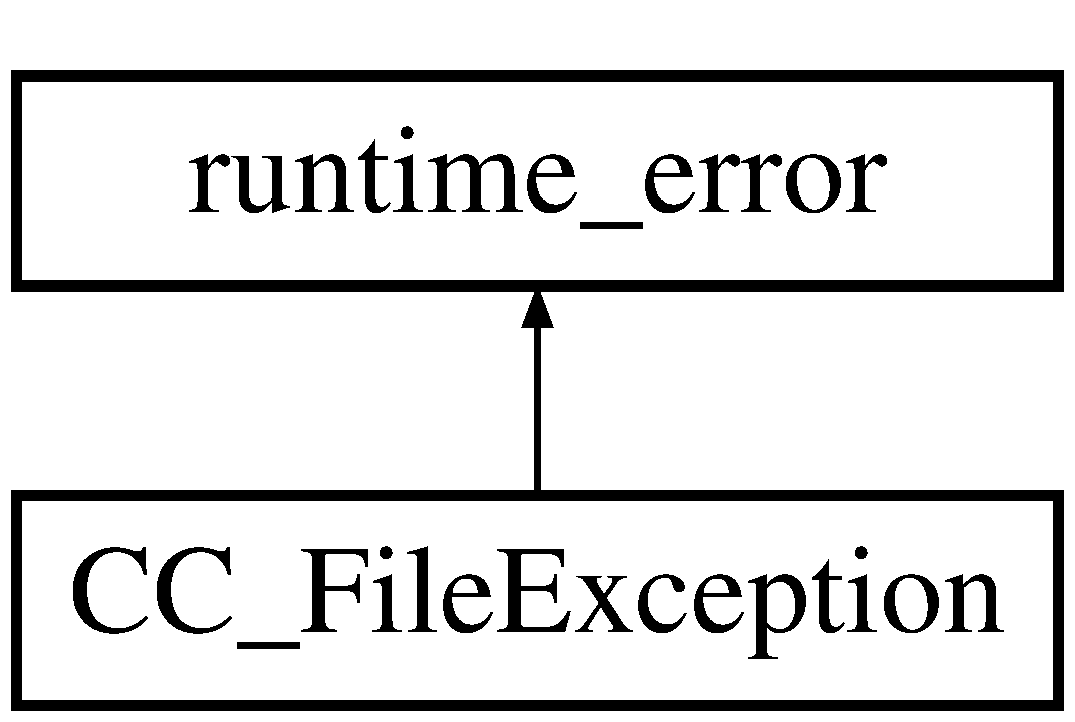
\includegraphics[height=2.000000cm]{a00032}
\end{center}
\end{figure}
\subsection*{Public Member Functions}
\begin{DoxyCompactItemize}
\item 
\hyperlink{a00032_abc5e91a9fd849864dcc3373a861fc90c}{C\-C\-\_\-\-File\-Exception} (const std\-::string \&reason)
\item 
\hyperlink{a00032_a93a9898ff8ffc0b3eb8b5ca9c9e2c02b}{C\-C\-\_\-\-File\-Exception} (uint32\-\_\-t name\-I\-D)
\end{DoxyCompactItemize}
\subsection*{Static Private Member Functions}
\begin{DoxyCompactItemize}
\item 
static std\-::string \hyperlink{a00032_a0acb55e721eb225c8076584a2e5f8dcd}{Get\-Error\-From\-I\-D} (uint32\-\_\-t name\-I\-D)
\end{DoxyCompactItemize}


\subsection{Constructor \& Destructor Documentation}
\hypertarget{a00032_abc5e91a9fd849864dcc3373a861fc90c}{\index{C\-C\-\_\-\-File\-Exception@{C\-C\-\_\-\-File\-Exception}!C\-C\-\_\-\-File\-Exception@{C\-C\-\_\-\-File\-Exception}}
\index{C\-C\-\_\-\-File\-Exception@{C\-C\-\_\-\-File\-Exception}!CC_FileException@{C\-C\-\_\-\-File\-Exception}}
\subsubsection[{C\-C\-\_\-\-File\-Exception}]{\setlength{\rightskip}{0pt plus 5cm}C\-C\-\_\-\-File\-Exception\-::\-C\-C\-\_\-\-File\-Exception (
\begin{DoxyParamCaption}
\item[{const std\-::string \&}]{reason}
\end{DoxyParamCaption}
)\hspace{0.3cm}{\ttfamily [inline]}}}\label{a00032_abc5e91a9fd849864dcc3373a861fc90c}
\hypertarget{a00032_a93a9898ff8ffc0b3eb8b5ca9c9e2c02b}{\index{C\-C\-\_\-\-File\-Exception@{C\-C\-\_\-\-File\-Exception}!C\-C\-\_\-\-File\-Exception@{C\-C\-\_\-\-File\-Exception}}
\index{C\-C\-\_\-\-File\-Exception@{C\-C\-\_\-\-File\-Exception}!CC_FileException@{C\-C\-\_\-\-File\-Exception}}
\subsubsection[{C\-C\-\_\-\-File\-Exception}]{\setlength{\rightskip}{0pt plus 5cm}C\-C\-\_\-\-File\-Exception\-::\-C\-C\-\_\-\-File\-Exception (
\begin{DoxyParamCaption}
\item[{uint32\-\_\-t}]{name\-I\-D}
\end{DoxyParamCaption}
)\hspace{0.3cm}{\ttfamily [inline]}}}\label{a00032_a93a9898ff8ffc0b3eb8b5ca9c9e2c02b}


\subsection{Member Function Documentation}
\hypertarget{a00032_a0acb55e721eb225c8076584a2e5f8dcd}{\index{C\-C\-\_\-\-File\-Exception@{C\-C\-\_\-\-File\-Exception}!Get\-Error\-From\-I\-D@{Get\-Error\-From\-I\-D}}
\index{Get\-Error\-From\-I\-D@{Get\-Error\-From\-I\-D}!CC_FileException@{C\-C\-\_\-\-File\-Exception}}
\subsubsection[{Get\-Error\-From\-I\-D}]{\setlength{\rightskip}{0pt plus 5cm}static std\-::string C\-C\-\_\-\-File\-Exception\-::\-Get\-Error\-From\-I\-D (
\begin{DoxyParamCaption}
\item[{uint32\-\_\-t}]{name\-I\-D}
\end{DoxyParamCaption}
)\hspace{0.3cm}{\ttfamily [inline]}, {\ttfamily [static]}, {\ttfamily [private]}}}\label{a00032_a0acb55e721eb225c8076584a2e5f8dcd}


The documentation for this class was generated from the following file\-:\begin{DoxyCompactItemize}
\item 
src/core/\hyperlink{a00206}{cc\-\_\-fileformat.\-h}\end{DoxyCompactItemize}

\hypertarget{a00033}{\section{C\-C\-\_\-lasso Class Reference}
\label{a00033}\index{C\-C\-\_\-lasso@{C\-C\-\_\-lasso}}
}


{\ttfamily \#include $<$cc\-\_\-shapes.\-h$>$}

Inheritance diagram for C\-C\-\_\-lasso\-:\begin{figure}[H]
\begin{center}
\leavevmode
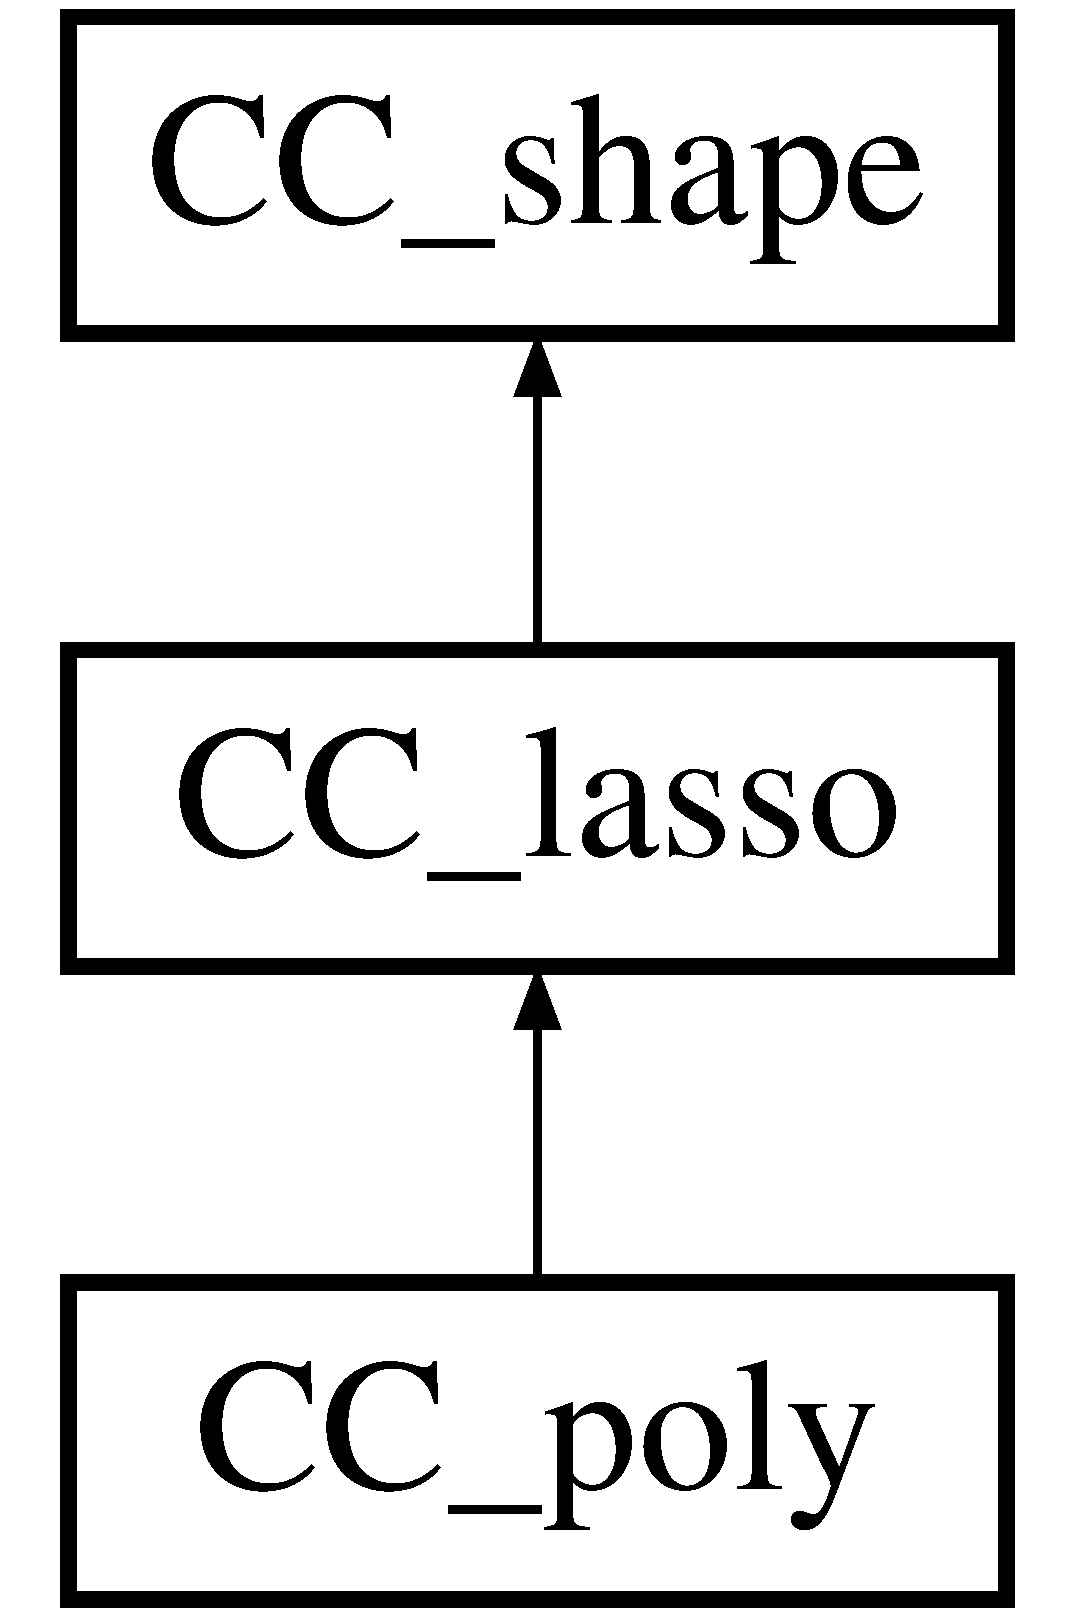
\includegraphics[height=3.000000cm]{a00033}
\end{center}
\end{figure}
\subsection*{Public Member Functions}
\begin{DoxyCompactItemize}
\item 
\hyperlink{a00033_a52c0140bc457076fd9d0126d3dc1c8ad}{C\-C\-\_\-lasso} (const \hyperlink{a00029}{C\-C\-\_\-coord} \&p)
\item 
virtual \hyperlink{a00033_a20774b6bda8264fe9e229a0bbf9854f7}{$\sim$\-C\-C\-\_\-lasso} ()
\item 
virtual void \hyperlink{a00033_ae5572606390286f5b6a2f137aee93dc9}{On\-Move} (const \hyperlink{a00029}{C\-C\-\_\-coord} \&p, const \hyperlink{a00029}{C\-C\-\_\-coord} \&snapped\-\_\-p)
\item 
void \hyperlink{a00033_afe2140061e67412e38f86c13226c33b5}{Clear} ()
\item 
void \hyperlink{a00033_a69c7a48f5b32a35407dafdcabd62cc1d}{Start} (const \hyperlink{a00029}{C\-C\-\_\-coord} \&p)
\item 
void \hyperlink{a00033_a86d2e800ef81566eb90d9d5819d7bcde}{End} ()
\item 
void \hyperlink{a00033_a8d6269272f544d58e85deb5fee9f04f4}{Append} (const \hyperlink{a00029}{C\-C\-\_\-coord} \&p)
\item 
bool \hyperlink{a00033_a6cdc0697c525220754dd53777587ea72}{Inside} (const \hyperlink{a00029}{C\-C\-\_\-coord} \&p) const 
\item 
virtual std\-::vector\\*
$<$ \hyperlink{a00031}{C\-C\-\_\-\-Draw\-Command} $>$ \hyperlink{a00033_afa75847821de1281822ec0ca1521e7f5}{Get\-C\-C\-\_\-\-Draw\-Command} (float x, float y) const 
\item 
void \hyperlink{a00033_ac36fdd2ff053803544c32ee860690d77}{Drag} (const \hyperlink{a00029}{C\-C\-\_\-coord} \&p)
\item 
const \hyperlink{a00029}{C\-C\-\_\-coord} $\ast$ \hyperlink{a00033_a7fc031e0de063742c0537052f395cc29}{First\-Point} () const 
\end{DoxyCompactItemize}
\subsection*{Private Types}
\begin{DoxyCompactItemize}
\item 
typedef std\-::vector$<$ \hyperlink{a00029}{C\-C\-\_\-coord} $>$ \hyperlink{a00033_a6c1ecccf9e723b7179aaf286dd7ba715}{Point\-List}
\end{DoxyCompactItemize}
\subsection*{Private Member Functions}
\begin{DoxyCompactItemize}
\item 
bool \hyperlink{a00033_a54ad0a354040f6d9f4a12b7e355f45f9}{Crosses\-Line} (const \hyperlink{a00029}{C\-C\-\_\-coord} \&start, const \hyperlink{a00029}{C\-C\-\_\-coord} \&end, const \hyperlink{a00029}{C\-C\-\_\-coord} \&p) const 
\end{DoxyCompactItemize}
\subsection*{Private Attributes}
\begin{DoxyCompactItemize}
\item 
\hyperlink{a00033_a6c1ecccf9e723b7179aaf286dd7ba715}{Point\-List} \hyperlink{a00033_aa2fba003c26aa52be0c935482a86ce5b}{pntlist}
\end{DoxyCompactItemize}


\subsection{Member Typedef Documentation}
\hypertarget{a00033_a6c1ecccf9e723b7179aaf286dd7ba715}{\index{C\-C\-\_\-lasso@{C\-C\-\_\-lasso}!Point\-List@{Point\-List}}
\index{Point\-List@{Point\-List}!CC_lasso@{C\-C\-\_\-lasso}}
\subsubsection[{Point\-List}]{\setlength{\rightskip}{0pt plus 5cm}typedef std\-::vector$<${\bf C\-C\-\_\-coord}$>$ {\bf C\-C\-\_\-lasso\-::\-Point\-List}\hspace{0.3cm}{\ttfamily [private]}}}\label{a00033_a6c1ecccf9e723b7179aaf286dd7ba715}


\subsection{Constructor \& Destructor Documentation}
\hypertarget{a00033_a52c0140bc457076fd9d0126d3dc1c8ad}{\index{C\-C\-\_\-lasso@{C\-C\-\_\-lasso}!C\-C\-\_\-lasso@{C\-C\-\_\-lasso}}
\index{C\-C\-\_\-lasso@{C\-C\-\_\-lasso}!CC_lasso@{C\-C\-\_\-lasso}}
\subsubsection[{C\-C\-\_\-lasso}]{\setlength{\rightskip}{0pt plus 5cm}C\-C\-\_\-lasso\-::\-C\-C\-\_\-lasso (
\begin{DoxyParamCaption}
\item[{const {\bf C\-C\-\_\-coord} \&}]{p}
\end{DoxyParamCaption}
)}}\label{a00033_a52c0140bc457076fd9d0126d3dc1c8ad}
\hypertarget{a00033_a20774b6bda8264fe9e229a0bbf9854f7}{\index{C\-C\-\_\-lasso@{C\-C\-\_\-lasso}!$\sim$\-C\-C\-\_\-lasso@{$\sim$\-C\-C\-\_\-lasso}}
\index{$\sim$\-C\-C\-\_\-lasso@{$\sim$\-C\-C\-\_\-lasso}!CC_lasso@{C\-C\-\_\-lasso}}
\subsubsection[{$\sim$\-C\-C\-\_\-lasso}]{\setlength{\rightskip}{0pt plus 5cm}C\-C\-\_\-lasso\-::$\sim$\-C\-C\-\_\-lasso (
\begin{DoxyParamCaption}
{}
\end{DoxyParamCaption}
)\hspace{0.3cm}{\ttfamily [virtual]}}}\label{a00033_a20774b6bda8264fe9e229a0bbf9854f7}


\subsection{Member Function Documentation}
\hypertarget{a00033_a8d6269272f544d58e85deb5fee9f04f4}{\index{C\-C\-\_\-lasso@{C\-C\-\_\-lasso}!Append@{Append}}
\index{Append@{Append}!CC_lasso@{C\-C\-\_\-lasso}}
\subsubsection[{Append}]{\setlength{\rightskip}{0pt plus 5cm}void C\-C\-\_\-lasso\-::\-Append (
\begin{DoxyParamCaption}
\item[{const {\bf C\-C\-\_\-coord} \&}]{p}
\end{DoxyParamCaption}
)}}\label{a00033_a8d6269272f544d58e85deb5fee9f04f4}
\hypertarget{a00033_afe2140061e67412e38f86c13226c33b5}{\index{C\-C\-\_\-lasso@{C\-C\-\_\-lasso}!Clear@{Clear}}
\index{Clear@{Clear}!CC_lasso@{C\-C\-\_\-lasso}}
\subsubsection[{Clear}]{\setlength{\rightskip}{0pt plus 5cm}void C\-C\-\_\-lasso\-::\-Clear (
\begin{DoxyParamCaption}
{}
\end{DoxyParamCaption}
)}}\label{a00033_afe2140061e67412e38f86c13226c33b5}
\hypertarget{a00033_a54ad0a354040f6d9f4a12b7e355f45f9}{\index{C\-C\-\_\-lasso@{C\-C\-\_\-lasso}!Crosses\-Line@{Crosses\-Line}}
\index{Crosses\-Line@{Crosses\-Line}!CC_lasso@{C\-C\-\_\-lasso}}
\subsubsection[{Crosses\-Line}]{\setlength{\rightskip}{0pt plus 5cm}bool C\-C\-\_\-lasso\-::\-Crosses\-Line (
\begin{DoxyParamCaption}
\item[{const {\bf C\-C\-\_\-coord} \&}]{start, }
\item[{const {\bf C\-C\-\_\-coord} \&}]{end, }
\item[{const {\bf C\-C\-\_\-coord} \&}]{p}
\end{DoxyParamCaption}
) const\hspace{0.3cm}{\ttfamily [private]}}}\label{a00033_a54ad0a354040f6d9f4a12b7e355f45f9}
\hypertarget{a00033_ac36fdd2ff053803544c32ee860690d77}{\index{C\-C\-\_\-lasso@{C\-C\-\_\-lasso}!Drag@{Drag}}
\index{Drag@{Drag}!CC_lasso@{C\-C\-\_\-lasso}}
\subsubsection[{Drag}]{\setlength{\rightskip}{0pt plus 5cm}void C\-C\-\_\-lasso\-::\-Drag (
\begin{DoxyParamCaption}
\item[{const {\bf C\-C\-\_\-coord} \&}]{p}
\end{DoxyParamCaption}
)}}\label{a00033_ac36fdd2ff053803544c32ee860690d77}
\hypertarget{a00033_a86d2e800ef81566eb90d9d5819d7bcde}{\index{C\-C\-\_\-lasso@{C\-C\-\_\-lasso}!End@{End}}
\index{End@{End}!CC_lasso@{C\-C\-\_\-lasso}}
\subsubsection[{End}]{\setlength{\rightskip}{0pt plus 5cm}void C\-C\-\_\-lasso\-::\-End (
\begin{DoxyParamCaption}
{}
\end{DoxyParamCaption}
)}}\label{a00033_a86d2e800ef81566eb90d9d5819d7bcde}
\hypertarget{a00033_a7fc031e0de063742c0537052f395cc29}{\index{C\-C\-\_\-lasso@{C\-C\-\_\-lasso}!First\-Point@{First\-Point}}
\index{First\-Point@{First\-Point}!CC_lasso@{C\-C\-\_\-lasso}}
\subsubsection[{First\-Point}]{\setlength{\rightskip}{0pt plus 5cm}const {\bf C\-C\-\_\-coord}$\ast$ C\-C\-\_\-lasso\-::\-First\-Point (
\begin{DoxyParamCaption}
{}
\end{DoxyParamCaption}
) const\hspace{0.3cm}{\ttfamily [inline]}}}\label{a00033_a7fc031e0de063742c0537052f395cc29}
\hypertarget{a00033_afa75847821de1281822ec0ca1521e7f5}{\index{C\-C\-\_\-lasso@{C\-C\-\_\-lasso}!Get\-C\-C\-\_\-\-Draw\-Command@{Get\-C\-C\-\_\-\-Draw\-Command}}
\index{Get\-C\-C\-\_\-\-Draw\-Command@{Get\-C\-C\-\_\-\-Draw\-Command}!CC_lasso@{C\-C\-\_\-lasso}}
\subsubsection[{Get\-C\-C\-\_\-\-Draw\-Command}]{\setlength{\rightskip}{0pt plus 5cm}std\-::vector$<$ {\bf C\-C\-\_\-\-Draw\-Command} $>$ C\-C\-\_\-lasso\-::\-Get\-C\-C\-\_\-\-Draw\-Command (
\begin{DoxyParamCaption}
\item[{float}]{x, }
\item[{float}]{y}
\end{DoxyParamCaption}
) const\hspace{0.3cm}{\ttfamily [virtual]}}}\label{a00033_afa75847821de1281822ec0ca1521e7f5}


Implements \hyperlink{a00037_aec026dc3fefc83bd03031e17307d073c}{C\-C\-\_\-shape}.

\hypertarget{a00033_a6cdc0697c525220754dd53777587ea72}{\index{C\-C\-\_\-lasso@{C\-C\-\_\-lasso}!Inside@{Inside}}
\index{Inside@{Inside}!CC_lasso@{C\-C\-\_\-lasso}}
\subsubsection[{Inside}]{\setlength{\rightskip}{0pt plus 5cm}bool C\-C\-\_\-lasso\-::\-Inside (
\begin{DoxyParamCaption}
\item[{const {\bf C\-C\-\_\-coord} \&}]{p}
\end{DoxyParamCaption}
) const}}\label{a00033_a6cdc0697c525220754dd53777587ea72}
\hypertarget{a00033_ae5572606390286f5b6a2f137aee93dc9}{\index{C\-C\-\_\-lasso@{C\-C\-\_\-lasso}!On\-Move@{On\-Move}}
\index{On\-Move@{On\-Move}!CC_lasso@{C\-C\-\_\-lasso}}
\subsubsection[{On\-Move}]{\setlength{\rightskip}{0pt plus 5cm}void C\-C\-\_\-lasso\-::\-On\-Move (
\begin{DoxyParamCaption}
\item[{const {\bf C\-C\-\_\-coord} \&}]{p, }
\item[{const {\bf C\-C\-\_\-coord} \&}]{snapped\-\_\-p}
\end{DoxyParamCaption}
)\hspace{0.3cm}{\ttfamily [virtual]}}}\label{a00033_ae5572606390286f5b6a2f137aee93dc9}


Implements \hyperlink{a00037_a323c027fc21841c560b5759573b50f56}{C\-C\-\_\-shape}.



Reimplemented in \hyperlink{a00036_aaa87ba1cbd1a87b6d1602945c6013dd2}{C\-C\-\_\-poly}.

\hypertarget{a00033_a69c7a48f5b32a35407dafdcabd62cc1d}{\index{C\-C\-\_\-lasso@{C\-C\-\_\-lasso}!Start@{Start}}
\index{Start@{Start}!CC_lasso@{C\-C\-\_\-lasso}}
\subsubsection[{Start}]{\setlength{\rightskip}{0pt plus 5cm}void C\-C\-\_\-lasso\-::\-Start (
\begin{DoxyParamCaption}
\item[{const {\bf C\-C\-\_\-coord} \&}]{p}
\end{DoxyParamCaption}
)}}\label{a00033_a69c7a48f5b32a35407dafdcabd62cc1d}


\subsection{Member Data Documentation}
\hypertarget{a00033_aa2fba003c26aa52be0c935482a86ce5b}{\index{C\-C\-\_\-lasso@{C\-C\-\_\-lasso}!pntlist@{pntlist}}
\index{pntlist@{pntlist}!CC_lasso@{C\-C\-\_\-lasso}}
\subsubsection[{pntlist}]{\setlength{\rightskip}{0pt plus 5cm}{\bf Point\-List} C\-C\-\_\-lasso\-::pntlist\hspace{0.3cm}{\ttfamily [private]}}}\label{a00033_aa2fba003c26aa52be0c935482a86ce5b}


The documentation for this class was generated from the following files\-:\begin{DoxyCompactItemize}
\item 
src/core/\hyperlink{a00210}{cc\-\_\-shapes.\-h}\item 
src/core/\hyperlink{a00209}{cc\-\_\-shapes.\-cpp}\end{DoxyCompactItemize}

\hypertarget{a00034}{\section{C\-C\-\_\-point Class Reference}
\label{a00034}\index{C\-C\-\_\-point@{C\-C\-\_\-point}}
}


This class represents a point in a.  




{\ttfamily \#include $<$cc\-\_\-point.\-h$>$}

\subsection*{Public Member Functions}
\begin{DoxyCompactItemize}
\item 
\hyperlink{a00034_aca83bde44f92cd505fc2bd1d2cae2ade}{C\-C\-\_\-point} ()
\begin{DoxyCompactList}\small\item\em Makes a plain dot, with a null position and uninitialized reference points. \end{DoxyCompactList}\item 
\hyperlink{a00034_a5cf13d3ea61c85cdcb44048e3be9b9d5}{C\-C\-\_\-point} (const \hyperlink{a00029}{C\-C\-\_\-coord} \&pos)
\begin{DoxyCompactList}\small\item\em Makes a plain dot located at the position provided in the parameters. \end{DoxyCompactList}\item 
\hyperlink{a00034_ae8a3a993cb0e38634f347af41ede4594}{C\-C\-\_\-point} (const std\-::vector$<$ uint8\-\_\-t $>$ \&serialized\-\_\-data)
\begin{DoxyCompactList}\small\item\em Used to load a point from a file. \end{DoxyCompactList}\item 
std\-::vector$<$ uint8\-\_\-t $>$ \hyperlink{a00034_a2de2c8ccca571f59abaf282a2c44a7e5}{Serialize} () const 
\begin{DoxyCompactList}\small\item\em Generates a serialized version of this point to be saved in a file. \end{DoxyCompactList}\item 
bool \hyperlink{a00034_adb7c6247e92c09adcc068dad928db579}{Get\-Flip} () const 
\begin{DoxyCompactList}\small\item\em Returns true if the label on the dot is flipped. \end{DoxyCompactList}\item 
void \hyperlink{a00034_ab13b2611cdb23e13c1cb8231d0ab73ff}{Flip} (bool val=true)
\begin{DoxyCompactList}\small\item\em Indicates which side of the dot that the label should be located in the viewer (that is, indicates whether or not the label of this dot is flipped). \end{DoxyCompactList}\item 
void \hyperlink{a00034_ae593f6c7994bcec3b30b5b1f9744d098}{Flip\-Toggle} ()
\begin{DoxyCompactList}\small\item\em Toggles whether or not the label of the dot is flipped in the viewer. \end{DoxyCompactList}\item 
\hyperlink{a00216_a68cd84e0300be6f9ff4474682762c9ee}{S\-Y\-M\-B\-O\-L\-\_\-\-T\-Y\-P\-E} \hyperlink{a00034_ab87115812c129465788ae5da5d684110}{Get\-Symbol} () const 
\begin{DoxyCompactList}\small\item\em Returns the symbol associated with this dot (e.\-g. \end{DoxyCompactList}\item 
void \hyperlink{a00034_ad797e691ddb9b681a8b204de3ee87e33}{Set\-Symbol} (\hyperlink{a00216_a68cd84e0300be6f9ff4474682762c9ee}{S\-Y\-M\-B\-O\-L\-\_\-\-T\-Y\-P\-E} sym)
\begin{DoxyCompactList}\small\item\em Sets the symbol associated with this dot. \end{DoxyCompactList}\item 
\hyperlink{a00029}{C\-C\-\_\-coord} \hyperlink{a00034_aa969cddcae9eb35d23b38829775927c7}{Get\-Pos} (unsigned ref=0) const 
\item 
void \hyperlink{a00034_aea2566cb1dd1c1bbde6ce83150462037}{Set\-Pos} (const \hyperlink{a00029}{C\-C\-\_\-coord} \&c, unsigned ref=0)
\end{DoxyCompactItemize}
\subsection*{Static Public Attributes}
\begin{DoxyCompactItemize}
\item 
static const unsigned \hyperlink{a00034_a2b34de427e5864328fd455f3122d96f4}{k\-Num\-Ref\-Points} = 3
\begin{DoxyCompactList}\small\item\em The number of reference points associated with each point. \end{DoxyCompactList}\end{DoxyCompactItemize}
\subsection*{Private Types}
\begin{DoxyCompactItemize}
\item 
enum \{ \hyperlink{a00034_aa09d4a78d659a5809cc4ca1e7022c84aac11f0df078c0ced8c4de839952fbe1e8}{k\-Point\-Label\-Flipped}, 
\hyperlink{a00034_aa09d4a78d659a5809cc4ca1e7022c84aac65d0716d4049256924dd894d9935221}{k\-Total\-Bits}
 \}
\end{DoxyCompactItemize}
\subsection*{Private Attributes}
\begin{DoxyCompactItemize}
\item 
std\-::bitset$<$ \hyperlink{a00034_aa09d4a78d659a5809cc4ca1e7022c84aac65d0716d4049256924dd894d9935221}{k\-Total\-Bits} $>$ \hyperlink{a00034_a676172a1cc4a700a9c3662155c8b06a8}{m\-Flags}
\item 
\hyperlink{a00216_a68cd84e0300be6f9ff4474682762c9ee}{S\-Y\-M\-B\-O\-L\-\_\-\-T\-Y\-P\-E} \hyperlink{a00034_a43c6a5906d61451a1bc48635faf44721}{m\-Sym}
\item 
\hyperlink{a00029}{C\-C\-\_\-coord} \hyperlink{a00034_a01cdfaad90c4b25418c94e3e17e119a1}{m\-Pos}
\item 
\hyperlink{a00029}{C\-C\-\_\-coord} \hyperlink{a00034_acb88e94b06850fed4fb44fa9fe095fc0}{m\-Ref} \mbox{[}\hyperlink{a00034_a2b34de427e5864328fd455f3122d96f4}{k\-Num\-Ref\-Points}\mbox{]}
\end{DoxyCompactItemize}
\subsection*{Friends}
\begin{DoxyCompactItemize}
\item 
struct \hyperlink{a00034_ab0f18edc2251918b5602d8a471f2ecc0}{C\-C\-\_\-point\-\_\-values}
\item 
bool \hyperlink{a00034_a83253bab8cb644ce0049e6bc659c22c5}{Check\-\_\-\-C\-C\-\_\-point} (const \hyperlink{a00034}{C\-C\-\_\-point} \&, const struct \hyperlink{a00035}{C\-C\-\_\-point\-\_\-values} \&)
\end{DoxyCompactItemize}


\subsection{Detailed Description}
This class represents a point in a. 

\subsection{Member Enumeration Documentation}
\hypertarget{a00034_aa09d4a78d659a5809cc4ca1e7022c84a}{\subsubsection[{anonymous enum}]{\setlength{\rightskip}{0pt plus 5cm}anonymous enum\hspace{0.3cm}{\ttfamily [private]}}}\label{a00034_aa09d4a78d659a5809cc4ca1e7022c84a}
\begin{Desc}
\item[Enumerator]\par
\begin{description}
\index{k\-Point\-Label\-Flipped@{k\-Point\-Label\-Flipped}!C\-C\-\_\-point@{C\-C\-\_\-point}}\index{C\-C\-\_\-point@{C\-C\-\_\-point}!k\-Point\-Label\-Flipped@{k\-Point\-Label\-Flipped}}\item[{\em 
\hypertarget{a00034_aa09d4a78d659a5809cc4ca1e7022c84aac11f0df078c0ced8c4de839952fbe1e8}{k\-Point\-Label\-Flipped}\label{a00034_aa09d4a78d659a5809cc4ca1e7022c84aac11f0df078c0ced8c4de839952fbe1e8}
}]\index{k\-Total\-Bits@{k\-Total\-Bits}!C\-C\-\_\-point@{C\-C\-\_\-point}}\index{C\-C\-\_\-point@{C\-C\-\_\-point}!k\-Total\-Bits@{k\-Total\-Bits}}\item[{\em 
\hypertarget{a00034_aa09d4a78d659a5809cc4ca1e7022c84aac65d0716d4049256924dd894d9935221}{k\-Total\-Bits}\label{a00034_aa09d4a78d659a5809cc4ca1e7022c84aac65d0716d4049256924dd894d9935221}
}]\end{description}
\end{Desc}


\subsection{Constructor \& Destructor Documentation}
\hypertarget{a00034_aca83bde44f92cd505fc2bd1d2cae2ade}{\index{C\-C\-\_\-point@{C\-C\-\_\-point}!C\-C\-\_\-point@{C\-C\-\_\-point}}
\index{C\-C\-\_\-point@{C\-C\-\_\-point}!CC_point@{C\-C\-\_\-point}}
\subsubsection[{C\-C\-\_\-point}]{\setlength{\rightskip}{0pt plus 5cm}C\-C\-\_\-point\-::\-C\-C\-\_\-point (
\begin{DoxyParamCaption}
{}
\end{DoxyParamCaption}
)}}\label{a00034_aca83bde44f92cd505fc2bd1d2cae2ade}


Makes a plain dot, with a null position and uninitialized reference points. 

Take caution when using this constructor, because many of the member variables will be null for the new point. \hypertarget{a00034_a5cf13d3ea61c85cdcb44048e3be9b9d5}{\index{C\-C\-\_\-point@{C\-C\-\_\-point}!C\-C\-\_\-point@{C\-C\-\_\-point}}
\index{C\-C\-\_\-point@{C\-C\-\_\-point}!CC_point@{C\-C\-\_\-point}}
\subsubsection[{C\-C\-\_\-point}]{\setlength{\rightskip}{0pt plus 5cm}C\-C\-\_\-point\-::\-C\-C\-\_\-point (
\begin{DoxyParamCaption}
\item[{const {\bf C\-C\-\_\-coord} \&}]{pos}
\end{DoxyParamCaption}
)}}\label{a00034_a5cf13d3ea61c85cdcb44048e3be9b9d5}


Makes a plain dot located at the position provided in the parameters. 

The reference points for the point will also all be set to that same position. \hypertarget{a00034_ae8a3a993cb0e38634f347af41ede4594}{\index{C\-C\-\_\-point@{C\-C\-\_\-point}!C\-C\-\_\-point@{C\-C\-\_\-point}}
\index{C\-C\-\_\-point@{C\-C\-\_\-point}!CC_point@{C\-C\-\_\-point}}
\subsubsection[{C\-C\-\_\-point}]{\setlength{\rightskip}{0pt plus 5cm}C\-C\-\_\-point\-::\-C\-C\-\_\-point (
\begin{DoxyParamCaption}
\item[{const std\-::vector$<$ uint8\-\_\-t $>$ \&}]{serialized\-\_\-data}
\end{DoxyParamCaption}
)}}\label{a00034_ae8a3a993cb0e38634f347af41ede4594}


Used to load a point from a file. 

A file contains serialized data that describes a point, and this constructor uses that data to construct a point that is identical to the one that was saved. 

\subsection{Member Function Documentation}
\hypertarget{a00034_ab13b2611cdb23e13c1cb8231d0ab73ff}{\index{C\-C\-\_\-point@{C\-C\-\_\-point}!Flip@{Flip}}
\index{Flip@{Flip}!CC_point@{C\-C\-\_\-point}}
\subsubsection[{Flip}]{\setlength{\rightskip}{0pt plus 5cm}void C\-C\-\_\-point\-::\-Flip (
\begin{DoxyParamCaption}
\item[{bool}]{val = {\ttfamily true}}
\end{DoxyParamCaption}
)}}\label{a00034_ab13b2611cdb23e13c1cb8231d0ab73ff}


Indicates which side of the dot that the label should be located in the viewer (that is, indicates whether or not the label of this dot is flipped). 

\hypertarget{a00034_ae593f6c7994bcec3b30b5b1f9744d098}{\index{C\-C\-\_\-point@{C\-C\-\_\-point}!Flip\-Toggle@{Flip\-Toggle}}
\index{Flip\-Toggle@{Flip\-Toggle}!CC_point@{C\-C\-\_\-point}}
\subsubsection[{Flip\-Toggle}]{\setlength{\rightskip}{0pt plus 5cm}void C\-C\-\_\-point\-::\-Flip\-Toggle (
\begin{DoxyParamCaption}
{}
\end{DoxyParamCaption}
)}}\label{a00034_ae593f6c7994bcec3b30b5b1f9744d098}


Toggles whether or not the label of the dot is flipped in the viewer. 

\hypertarget{a00034_adb7c6247e92c09adcc068dad928db579}{\index{C\-C\-\_\-point@{C\-C\-\_\-point}!Get\-Flip@{Get\-Flip}}
\index{Get\-Flip@{Get\-Flip}!CC_point@{C\-C\-\_\-point}}
\subsubsection[{Get\-Flip}]{\setlength{\rightskip}{0pt plus 5cm}bool C\-C\-\_\-point\-::\-Get\-Flip (
\begin{DoxyParamCaption}
{}
\end{DoxyParamCaption}
) const}}\label{a00034_adb7c6247e92c09adcc068dad928db579}


Returns true if the label on the dot is flipped. 

\hypertarget{a00034_aa969cddcae9eb35d23b38829775927c7}{\index{C\-C\-\_\-point@{C\-C\-\_\-point}!Get\-Pos@{Get\-Pos}}
\index{Get\-Pos@{Get\-Pos}!CC_point@{C\-C\-\_\-point}}
\subsubsection[{Get\-Pos}]{\setlength{\rightskip}{0pt plus 5cm}{\bf C\-C\-\_\-coord} C\-C\-\_\-point\-::\-Get\-Pos (
\begin{DoxyParamCaption}
\item[{unsigned}]{ref = {\ttfamily 0}}
\end{DoxyParamCaption}
) const}}\label{a00034_aa969cddcae9eb35d23b38829775927c7}
\hypertarget{a00034_ab87115812c129465788ae5da5d684110}{\index{C\-C\-\_\-point@{C\-C\-\_\-point}!Get\-Symbol@{Get\-Symbol}}
\index{Get\-Symbol@{Get\-Symbol}!CC_point@{C\-C\-\_\-point}}
\subsubsection[{Get\-Symbol}]{\setlength{\rightskip}{0pt plus 5cm}{\bf S\-Y\-M\-B\-O\-L\-\_\-\-T\-Y\-P\-E} C\-C\-\_\-point\-::\-Get\-Symbol (
\begin{DoxyParamCaption}
{}
\end{DoxyParamCaption}
) const}}\label{a00034_ab87115812c129465788ae5da5d684110}


Returns the symbol associated with this dot (e.\-g. 

solid, slash, plain, etc.). \hypertarget{a00034_a2de2c8ccca571f59abaf282a2c44a7e5}{\index{C\-C\-\_\-point@{C\-C\-\_\-point}!Serialize@{Serialize}}
\index{Serialize@{Serialize}!CC_point@{C\-C\-\_\-point}}
\subsubsection[{Serialize}]{\setlength{\rightskip}{0pt plus 5cm}std\-::vector$<$ uint8\-\_\-t $>$ C\-C\-\_\-point\-::\-Serialize (
\begin{DoxyParamCaption}
{}
\end{DoxyParamCaption}
) const}}\label{a00034_a2de2c8ccca571f59abaf282a2c44a7e5}


Generates a serialized version of this point to be saved in a file. 

\hypertarget{a00034_aea2566cb1dd1c1bbde6ce83150462037}{\index{C\-C\-\_\-point@{C\-C\-\_\-point}!Set\-Pos@{Set\-Pos}}
\index{Set\-Pos@{Set\-Pos}!CC_point@{C\-C\-\_\-point}}
\subsubsection[{Set\-Pos}]{\setlength{\rightskip}{0pt plus 5cm}void C\-C\-\_\-point\-::\-Set\-Pos (
\begin{DoxyParamCaption}
\item[{const {\bf C\-C\-\_\-coord} \&}]{c, }
\item[{unsigned}]{ref = {\ttfamily 0}}
\end{DoxyParamCaption}
)}}\label{a00034_aea2566cb1dd1c1bbde6ce83150462037}
\hypertarget{a00034_ad797e691ddb9b681a8b204de3ee87e33}{\index{C\-C\-\_\-point@{C\-C\-\_\-point}!Set\-Symbol@{Set\-Symbol}}
\index{Set\-Symbol@{Set\-Symbol}!CC_point@{C\-C\-\_\-point}}
\subsubsection[{Set\-Symbol}]{\setlength{\rightskip}{0pt plus 5cm}void C\-C\-\_\-point\-::\-Set\-Symbol (
\begin{DoxyParamCaption}
\item[{{\bf S\-Y\-M\-B\-O\-L\-\_\-\-T\-Y\-P\-E}}]{sym}
\end{DoxyParamCaption}
)}}\label{a00034_ad797e691ddb9b681a8b204de3ee87e33}


Sets the symbol associated with this dot. 



\subsection{Friends And Related Function Documentation}
\hypertarget{a00034_ab0f18edc2251918b5602d8a471f2ecc0}{\index{C\-C\-\_\-point@{C\-C\-\_\-point}!C\-C\-\_\-point\-\_\-values@{C\-C\-\_\-point\-\_\-values}}
\index{C\-C\-\_\-point\-\_\-values@{C\-C\-\_\-point\-\_\-values}!CC_point@{C\-C\-\_\-point}}
\subsubsection[{C\-C\-\_\-point\-\_\-values}]{\setlength{\rightskip}{0pt plus 5cm}friend struct {\bf C\-C\-\_\-point\-\_\-values}\hspace{0.3cm}{\ttfamily [friend]}}}\label{a00034_ab0f18edc2251918b5602d8a471f2ecc0}
\hypertarget{a00034_a83253bab8cb644ce0049e6bc659c22c5}{\index{C\-C\-\_\-point@{C\-C\-\_\-point}!Check\-\_\-\-C\-C\-\_\-point@{Check\-\_\-\-C\-C\-\_\-point}}
\index{Check\-\_\-\-C\-C\-\_\-point@{Check\-\_\-\-C\-C\-\_\-point}!CC_point@{C\-C\-\_\-point}}
\subsubsection[{Check\-\_\-\-C\-C\-\_\-point}]{\setlength{\rightskip}{0pt plus 5cm}bool Check\-\_\-\-C\-C\-\_\-point (
\begin{DoxyParamCaption}
\item[{const {\bf C\-C\-\_\-point} \&}]{, }
\item[{const struct {\bf C\-C\-\_\-point\-\_\-values} \&}]{}
\end{DoxyParamCaption}
)\hspace{0.3cm}{\ttfamily [friend]}}}\label{a00034_a83253bab8cb644ce0049e6bc659c22c5}


\subsection{Member Data Documentation}
\hypertarget{a00034_a2b34de427e5864328fd455f3122d96f4}{\index{C\-C\-\_\-point@{C\-C\-\_\-point}!k\-Num\-Ref\-Points@{k\-Num\-Ref\-Points}}
\index{k\-Num\-Ref\-Points@{k\-Num\-Ref\-Points}!CC_point@{C\-C\-\_\-point}}
\subsubsection[{k\-Num\-Ref\-Points}]{\setlength{\rightskip}{0pt plus 5cm}const unsigned C\-C\-\_\-point\-::k\-Num\-Ref\-Points = 3\hspace{0.3cm}{\ttfamily [static]}}}\label{a00034_a2b34de427e5864328fd455f3122d96f4}


The number of reference points associated with each point. 

This must be at least 1, since the first ref point is the position of the dot. \hypertarget{a00034_a676172a1cc4a700a9c3662155c8b06a8}{\index{C\-C\-\_\-point@{C\-C\-\_\-point}!m\-Flags@{m\-Flags}}
\index{m\-Flags@{m\-Flags}!CC_point@{C\-C\-\_\-point}}
\subsubsection[{m\-Flags}]{\setlength{\rightskip}{0pt plus 5cm}std\-::bitset$<${\bf k\-Total\-Bits}$>$ C\-C\-\_\-point\-::m\-Flags\hspace{0.3cm}{\ttfamily [private]}}}\label{a00034_a676172a1cc4a700a9c3662155c8b06a8}
\hypertarget{a00034_a01cdfaad90c4b25418c94e3e17e119a1}{\index{C\-C\-\_\-point@{C\-C\-\_\-point}!m\-Pos@{m\-Pos}}
\index{m\-Pos@{m\-Pos}!CC_point@{C\-C\-\_\-point}}
\subsubsection[{m\-Pos}]{\setlength{\rightskip}{0pt plus 5cm}{\bf C\-C\-\_\-coord} C\-C\-\_\-point\-::m\-Pos\hspace{0.3cm}{\ttfamily [private]}}}\label{a00034_a01cdfaad90c4b25418c94e3e17e119a1}
\hypertarget{a00034_acb88e94b06850fed4fb44fa9fe095fc0}{\index{C\-C\-\_\-point@{C\-C\-\_\-point}!m\-Ref@{m\-Ref}}
\index{m\-Ref@{m\-Ref}!CC_point@{C\-C\-\_\-point}}
\subsubsection[{m\-Ref}]{\setlength{\rightskip}{0pt plus 5cm}{\bf C\-C\-\_\-coord} C\-C\-\_\-point\-::m\-Ref\mbox{[}{\bf k\-Num\-Ref\-Points}\mbox{]}\hspace{0.3cm}{\ttfamily [private]}}}\label{a00034_acb88e94b06850fed4fb44fa9fe095fc0}
\hypertarget{a00034_a43c6a5906d61451a1bc48635faf44721}{\index{C\-C\-\_\-point@{C\-C\-\_\-point}!m\-Sym@{m\-Sym}}
\index{m\-Sym@{m\-Sym}!CC_point@{C\-C\-\_\-point}}
\subsubsection[{m\-Sym}]{\setlength{\rightskip}{0pt plus 5cm}{\bf S\-Y\-M\-B\-O\-L\-\_\-\-T\-Y\-P\-E} C\-C\-\_\-point\-::m\-Sym\hspace{0.3cm}{\ttfamily [private]}}}\label{a00034_a43c6a5906d61451a1bc48635faf44721}


The documentation for this class was generated from the following files\-:\begin{DoxyCompactItemize}
\item 
src/core/\hyperlink{a00208}{cc\-\_\-point.\-h}\item 
src/core/\hyperlink{a00207}{cc\-\_\-point.\-cpp}\end{DoxyCompactItemize}

\hypertarget{a00035}{\section{C\-C\-\_\-point\-\_\-values Struct Reference}
\label{a00035}\index{C\-C\-\_\-point\-\_\-values@{C\-C\-\_\-point\-\_\-values}}
}
\subsection*{Public Attributes}
\begin{DoxyCompactItemize}
\item 
std\-::bitset$<$ \hyperlink{a00034_aa09d4a78d659a5809cc4ca1e7022c84aac65d0716d4049256924dd894d9935221}{C\-C\-\_\-point\-::k\-Total\-Bits} $>$ \hyperlink{a00035_aaba0cdfb77d6416849ad4cc44c49acb6}{m\-Flags}
\item 
\hyperlink{a00216_a68cd84e0300be6f9ff4474682762c9ee}{S\-Y\-M\-B\-O\-L\-\_\-\-T\-Y\-P\-E} \hyperlink{a00035_aecc6f13cb613498e3c307a4be4353075}{m\-Sym}
\item 
\hyperlink{a00029}{C\-C\-\_\-coord} \hyperlink{a00035_afd2d71183219ead4687efa86e8fa6904}{m\-Pos}
\item 
\hyperlink{a00029}{C\-C\-\_\-coord} \hyperlink{a00035_ab8797ebb0797a22c1d90091265c822f2}{m\-Ref} \mbox{[}\hyperlink{a00034_a2b34de427e5864328fd455f3122d96f4}{C\-C\-\_\-point\-::k\-Num\-Ref\-Points}\mbox{]}
\item 
bool \hyperlink{a00035_adbd7c0d6e0412fc07d964551bb2ad9a1}{Get\-Flip}
\end{DoxyCompactItemize}


\subsection{Member Data Documentation}
\hypertarget{a00035_adbd7c0d6e0412fc07d964551bb2ad9a1}{\index{C\-C\-\_\-point\-\_\-values@{C\-C\-\_\-point\-\_\-values}!Get\-Flip@{Get\-Flip}}
\index{Get\-Flip@{Get\-Flip}!CC_point_values@{C\-C\-\_\-point\-\_\-values}}
\subsubsection[{Get\-Flip}]{\setlength{\rightskip}{0pt plus 5cm}bool C\-C\-\_\-point\-\_\-values\-::\-Get\-Flip}}\label{a00035_adbd7c0d6e0412fc07d964551bb2ad9a1}
\hypertarget{a00035_aaba0cdfb77d6416849ad4cc44c49acb6}{\index{C\-C\-\_\-point\-\_\-values@{C\-C\-\_\-point\-\_\-values}!m\-Flags@{m\-Flags}}
\index{m\-Flags@{m\-Flags}!CC_point_values@{C\-C\-\_\-point\-\_\-values}}
\subsubsection[{m\-Flags}]{\setlength{\rightskip}{0pt plus 5cm}std\-::bitset$<${\bf C\-C\-\_\-point\-::k\-Total\-Bits}$>$ C\-C\-\_\-point\-\_\-values\-::m\-Flags}}\label{a00035_aaba0cdfb77d6416849ad4cc44c49acb6}
\hypertarget{a00035_afd2d71183219ead4687efa86e8fa6904}{\index{C\-C\-\_\-point\-\_\-values@{C\-C\-\_\-point\-\_\-values}!m\-Pos@{m\-Pos}}
\index{m\-Pos@{m\-Pos}!CC_point_values@{C\-C\-\_\-point\-\_\-values}}
\subsubsection[{m\-Pos}]{\setlength{\rightskip}{0pt plus 5cm}{\bf C\-C\-\_\-coord} C\-C\-\_\-point\-\_\-values\-::m\-Pos}}\label{a00035_afd2d71183219ead4687efa86e8fa6904}
\hypertarget{a00035_ab8797ebb0797a22c1d90091265c822f2}{\index{C\-C\-\_\-point\-\_\-values@{C\-C\-\_\-point\-\_\-values}!m\-Ref@{m\-Ref}}
\index{m\-Ref@{m\-Ref}!CC_point_values@{C\-C\-\_\-point\-\_\-values}}
\subsubsection[{m\-Ref}]{\setlength{\rightskip}{0pt plus 5cm}{\bf C\-C\-\_\-coord} C\-C\-\_\-point\-\_\-values\-::m\-Ref\mbox{[}{\bf C\-C\-\_\-point\-::k\-Num\-Ref\-Points}\mbox{]}}}\label{a00035_ab8797ebb0797a22c1d90091265c822f2}
\hypertarget{a00035_aecc6f13cb613498e3c307a4be4353075}{\index{C\-C\-\_\-point\-\_\-values@{C\-C\-\_\-point\-\_\-values}!m\-Sym@{m\-Sym}}
\index{m\-Sym@{m\-Sym}!CC_point_values@{C\-C\-\_\-point\-\_\-values}}
\subsubsection[{m\-Sym}]{\setlength{\rightskip}{0pt plus 5cm}{\bf S\-Y\-M\-B\-O\-L\-\_\-\-T\-Y\-P\-E} C\-C\-\_\-point\-\_\-values\-::m\-Sym}}\label{a00035_aecc6f13cb613498e3c307a4be4353075}


The documentation for this struct was generated from the following file\-:\begin{DoxyCompactItemize}
\item 
src/core/\hyperlink{a00207}{cc\-\_\-point.\-cpp}\end{DoxyCompactItemize}

\hypertarget{a00036}{\section{C\-C\-\_\-poly Class Reference}
\label{a00036}\index{C\-C\-\_\-poly@{C\-C\-\_\-poly}}
}


{\ttfamily \#include $<$cc\-\_\-shapes.\-h$>$}

Inheritance diagram for C\-C\-\_\-poly\-:\begin{figure}[H]
\begin{center}
\leavevmode
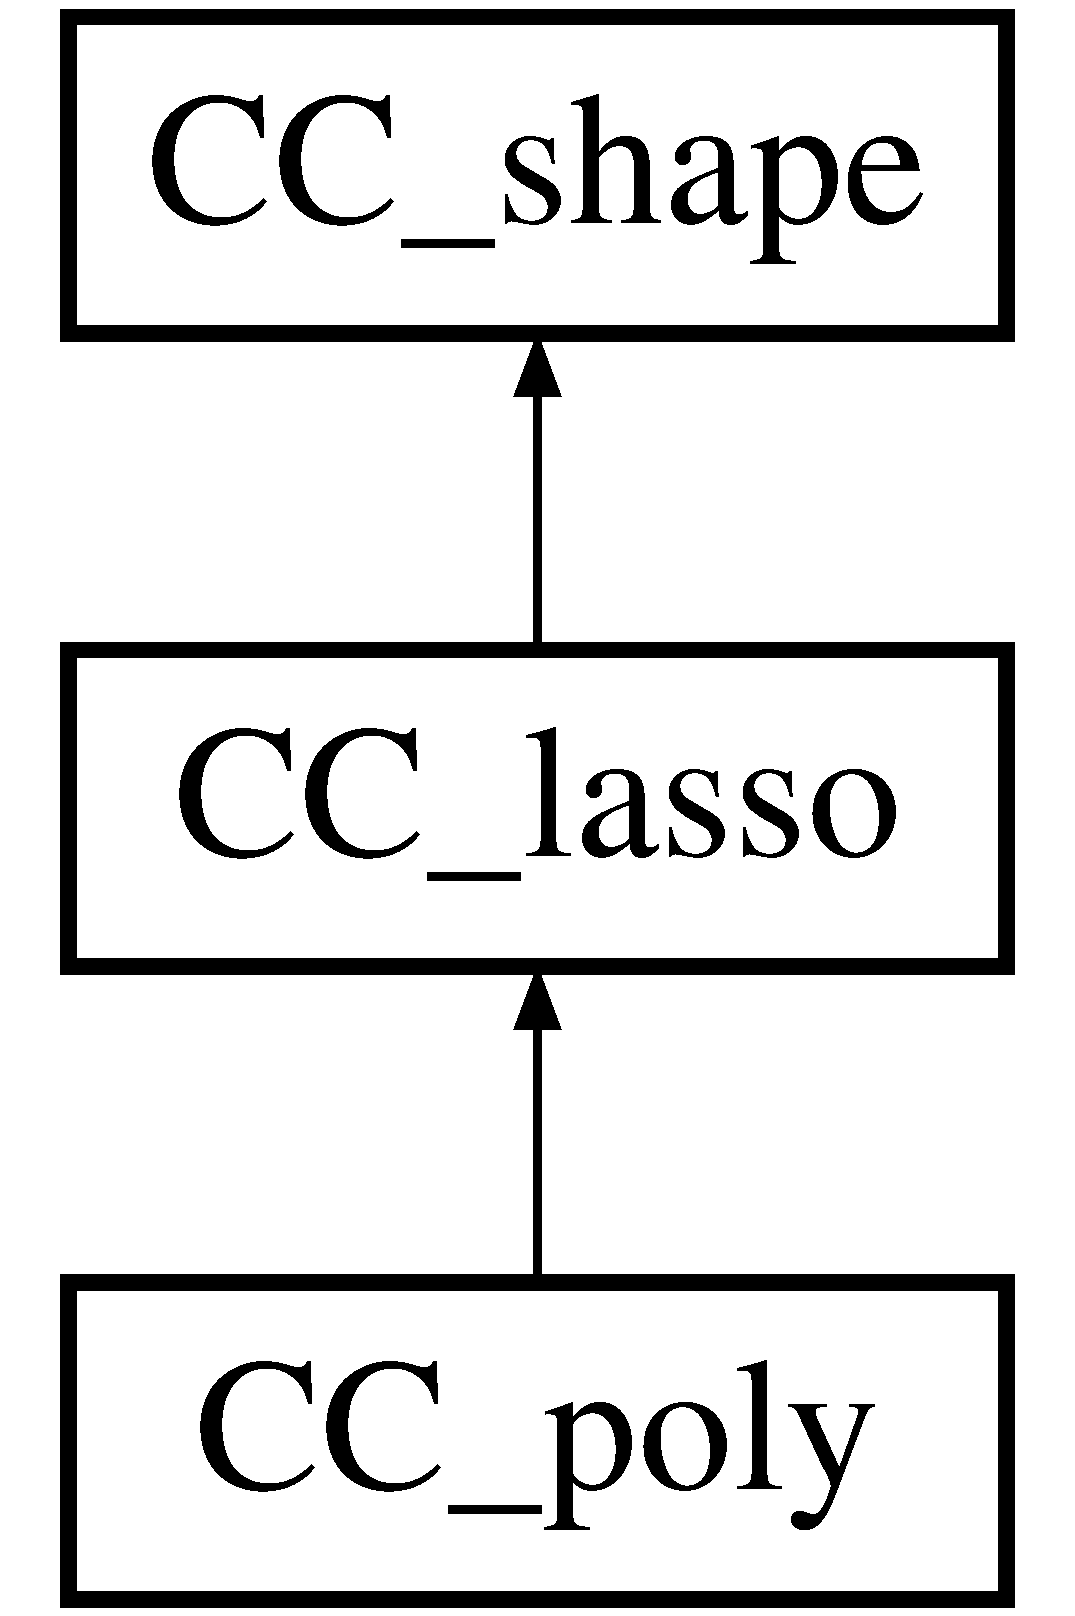
\includegraphics[height=3.000000cm]{a00036}
\end{center}
\end{figure}
\subsection*{Public Member Functions}
\begin{DoxyCompactItemize}
\item 
\hyperlink{a00036_ab45ac7dd4386f94ed27b20be9a4a51e4}{C\-C\-\_\-poly} (const \hyperlink{a00029}{C\-C\-\_\-coord} \&p)
\item 
virtual void \hyperlink{a00036_aaa87ba1cbd1a87b6d1602945c6013dd2}{On\-Move} (const \hyperlink{a00029}{C\-C\-\_\-coord} \&p, const \hyperlink{a00029}{C\-C\-\_\-coord} \&snapped\-\_\-p)
\end{DoxyCompactItemize}


\subsection{Constructor \& Destructor Documentation}
\hypertarget{a00036_ab45ac7dd4386f94ed27b20be9a4a51e4}{\index{C\-C\-\_\-poly@{C\-C\-\_\-poly}!C\-C\-\_\-poly@{C\-C\-\_\-poly}}
\index{C\-C\-\_\-poly@{C\-C\-\_\-poly}!CC_poly@{C\-C\-\_\-poly}}
\subsubsection[{C\-C\-\_\-poly}]{\setlength{\rightskip}{0pt plus 5cm}C\-C\-\_\-poly\-::\-C\-C\-\_\-poly (
\begin{DoxyParamCaption}
\item[{const {\bf C\-C\-\_\-coord} \&}]{p}
\end{DoxyParamCaption}
)}}\label{a00036_ab45ac7dd4386f94ed27b20be9a4a51e4}


\subsection{Member Function Documentation}
\hypertarget{a00036_aaa87ba1cbd1a87b6d1602945c6013dd2}{\index{C\-C\-\_\-poly@{C\-C\-\_\-poly}!On\-Move@{On\-Move}}
\index{On\-Move@{On\-Move}!CC_poly@{C\-C\-\_\-poly}}
\subsubsection[{On\-Move}]{\setlength{\rightskip}{0pt plus 5cm}void C\-C\-\_\-poly\-::\-On\-Move (
\begin{DoxyParamCaption}
\item[{const {\bf C\-C\-\_\-coord} \&}]{p, }
\item[{const {\bf C\-C\-\_\-coord} \&}]{snapped\-\_\-p}
\end{DoxyParamCaption}
)\hspace{0.3cm}{\ttfamily [virtual]}}}\label{a00036_aaa87ba1cbd1a87b6d1602945c6013dd2}


Reimplemented from \hyperlink{a00033_ae5572606390286f5b6a2f137aee93dc9}{C\-C\-\_\-lasso}.



The documentation for this class was generated from the following files\-:\begin{DoxyCompactItemize}
\item 
src/core/\hyperlink{a00210}{cc\-\_\-shapes.\-h}\item 
src/core/\hyperlink{a00209}{cc\-\_\-shapes.\-cpp}\end{DoxyCompactItemize}

\hypertarget{a00037}{\section{C\-C\-\_\-shape Class Reference}
\label{a00037}\index{C\-C\-\_\-shape@{C\-C\-\_\-shape}}
}


{\ttfamily \#include $<$cc\-\_\-shapes.\-h$>$}

Inheritance diagram for C\-C\-\_\-shape\-:\begin{figure}[H]
\begin{center}
\leavevmode
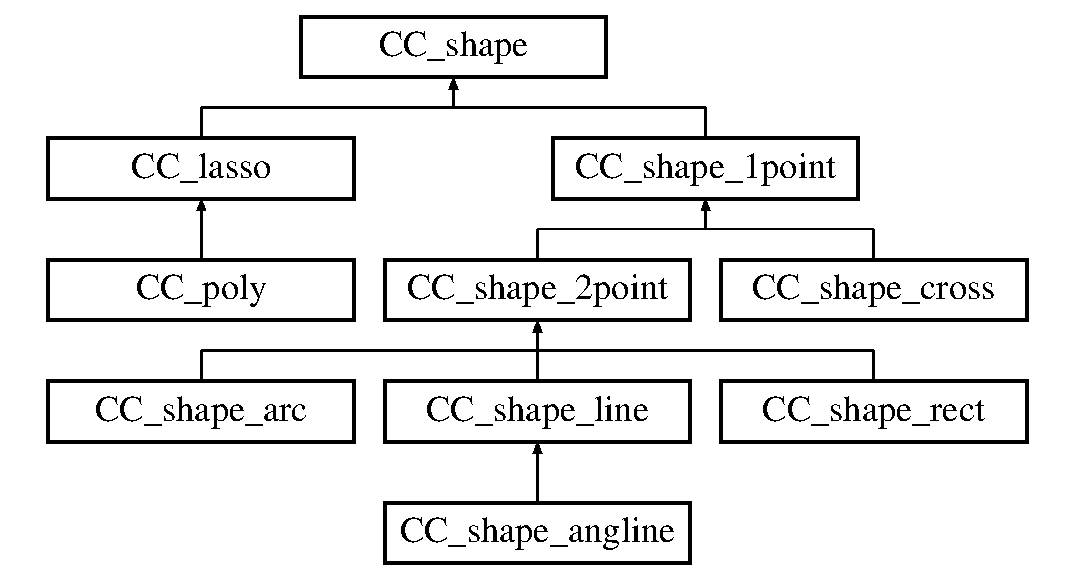
\includegraphics[height=5.000000cm]{a00037}
\end{center}
\end{figure}
\subsection*{Public Member Functions}
\begin{DoxyCompactItemize}
\item 
\hyperlink{a00037_a82a3842182b43479636e07051c01dc92}{C\-C\-\_\-shape} ()
\item 
virtual \hyperlink{a00037_a77face5d8bd1307231fe0b9bca2bd2d6}{$\sim$\-C\-C\-\_\-shape} ()
\item 
virtual std\-::vector\\*
$<$ \hyperlink{a00031}{C\-C\-\_\-\-Draw\-Command} $>$ \hyperlink{a00037_aec026dc3fefc83bd03031e17307d073c}{Get\-C\-C\-\_\-\-Draw\-Command} (float x, float y) const =0
\item 
virtual void \hyperlink{a00037_a323c027fc21841c560b5759573b50f56}{On\-Move} (const \hyperlink{a00029}{C\-C\-\_\-coord} \&p, const \hyperlink{a00029}{C\-C\-\_\-coord} \&snapped\-\_\-p)=0
\end{DoxyCompactItemize}


\subsection{Constructor \& Destructor Documentation}
\hypertarget{a00037_a82a3842182b43479636e07051c01dc92}{\index{C\-C\-\_\-shape@{C\-C\-\_\-shape}!C\-C\-\_\-shape@{C\-C\-\_\-shape}}
\index{C\-C\-\_\-shape@{C\-C\-\_\-shape}!CC_shape@{C\-C\-\_\-shape}}
\subsubsection[{C\-C\-\_\-shape}]{\setlength{\rightskip}{0pt plus 5cm}C\-C\-\_\-shape\-::\-C\-C\-\_\-shape (
\begin{DoxyParamCaption}
{}
\end{DoxyParamCaption}
)}}\label{a00037_a82a3842182b43479636e07051c01dc92}
\hypertarget{a00037_a77face5d8bd1307231fe0b9bca2bd2d6}{\index{C\-C\-\_\-shape@{C\-C\-\_\-shape}!$\sim$\-C\-C\-\_\-shape@{$\sim$\-C\-C\-\_\-shape}}
\index{$\sim$\-C\-C\-\_\-shape@{$\sim$\-C\-C\-\_\-shape}!CC_shape@{C\-C\-\_\-shape}}
\subsubsection[{$\sim$\-C\-C\-\_\-shape}]{\setlength{\rightskip}{0pt plus 5cm}C\-C\-\_\-shape\-::$\sim$\-C\-C\-\_\-shape (
\begin{DoxyParamCaption}
{}
\end{DoxyParamCaption}
)\hspace{0.3cm}{\ttfamily [virtual]}}}\label{a00037_a77face5d8bd1307231fe0b9bca2bd2d6}


\subsection{Member Function Documentation}
\hypertarget{a00037_aec026dc3fefc83bd03031e17307d073c}{\index{C\-C\-\_\-shape@{C\-C\-\_\-shape}!Get\-C\-C\-\_\-\-Draw\-Command@{Get\-C\-C\-\_\-\-Draw\-Command}}
\index{Get\-C\-C\-\_\-\-Draw\-Command@{Get\-C\-C\-\_\-\-Draw\-Command}!CC_shape@{C\-C\-\_\-shape}}
\subsubsection[{Get\-C\-C\-\_\-\-Draw\-Command}]{\setlength{\rightskip}{0pt plus 5cm}virtual std\-::vector$<${\bf C\-C\-\_\-\-Draw\-Command}$>$ C\-C\-\_\-shape\-::\-Get\-C\-C\-\_\-\-Draw\-Command (
\begin{DoxyParamCaption}
\item[{float}]{x, }
\item[{float}]{y}
\end{DoxyParamCaption}
) const\hspace{0.3cm}{\ttfamily [pure virtual]}}}\label{a00037_aec026dc3fefc83bd03031e17307d073c}


Implemented in \hyperlink{a00033_afa75847821de1281822ec0ca1521e7f5}{C\-C\-\_\-lasso}, \hyperlink{a00044_aca56590bb687ba94ce96b0c0e66116f7}{C\-C\-\_\-shape\-\_\-rect}, \hyperlink{a00041_aa8f4623a8093d5fb095912e2b13ccf80}{C\-C\-\_\-shape\-\_\-arc}, \hyperlink{a00043_a65124c0a0a223f45eb151b78c6f38ade}{C\-C\-\_\-shape\-\_\-line}, and \hyperlink{a00042_ad258d1e056279b8e1b37cc25ac286ed8}{C\-C\-\_\-shape\-\_\-cross}.

\hypertarget{a00037_a323c027fc21841c560b5759573b50f56}{\index{C\-C\-\_\-shape@{C\-C\-\_\-shape}!On\-Move@{On\-Move}}
\index{On\-Move@{On\-Move}!CC_shape@{C\-C\-\_\-shape}}
\subsubsection[{On\-Move}]{\setlength{\rightskip}{0pt plus 5cm}virtual void C\-C\-\_\-shape\-::\-On\-Move (
\begin{DoxyParamCaption}
\item[{const {\bf C\-C\-\_\-coord} \&}]{p, }
\item[{const {\bf C\-C\-\_\-coord} \&}]{snapped\-\_\-p}
\end{DoxyParamCaption}
)\hspace{0.3cm}{\ttfamily [pure virtual]}}}\label{a00037_a323c027fc21841c560b5759573b50f56}


Implemented in \hyperlink{a00036_aaa87ba1cbd1a87b6d1602945c6013dd2}{C\-C\-\_\-poly}, \hyperlink{a00033_ae5572606390286f5b6a2f137aee93dc9}{C\-C\-\_\-lasso}, \hyperlink{a00041_ac99e4b812a5eb489d29d324cd7dca7e5}{C\-C\-\_\-shape\-\_\-arc}, \hyperlink{a00040_a3aead16af5b691651d76d1d71138aae8}{C\-C\-\_\-shape\-\_\-angline}, \hyperlink{a00043_a8678d21e42e37bece16b3cac98241d98}{C\-C\-\_\-shape\-\_\-line}, \hyperlink{a00039_a5de0c111a1e2e01c7f2802333809b421}{C\-C\-\_\-shape\-\_\-2point}, \hyperlink{a00042_a3326faef7625f5edfad2e5ba09927b6d}{C\-C\-\_\-shape\-\_\-cross}, and \hyperlink{a00038_a7110a3e16f7375074baa18efb997060a}{C\-C\-\_\-shape\-\_\-1point}.



The documentation for this class was generated from the following files\-:\begin{DoxyCompactItemize}
\item 
src/core/\hyperlink{a00210}{cc\-\_\-shapes.\-h}\item 
src/core/\hyperlink{a00209}{cc\-\_\-shapes.\-cpp}\end{DoxyCompactItemize}

\hypertarget{a00038}{\section{C\-C\-\_\-shape\-\_\-1point Class Reference}
\label{a00038}\index{C\-C\-\_\-shape\-\_\-1point@{C\-C\-\_\-shape\-\_\-1point}}
}


{\ttfamily \#include $<$cc\-\_\-shapes.\-h$>$}

Inheritance diagram for C\-C\-\_\-shape\-\_\-1point\-:\begin{figure}[H]
\begin{center}
\leavevmode
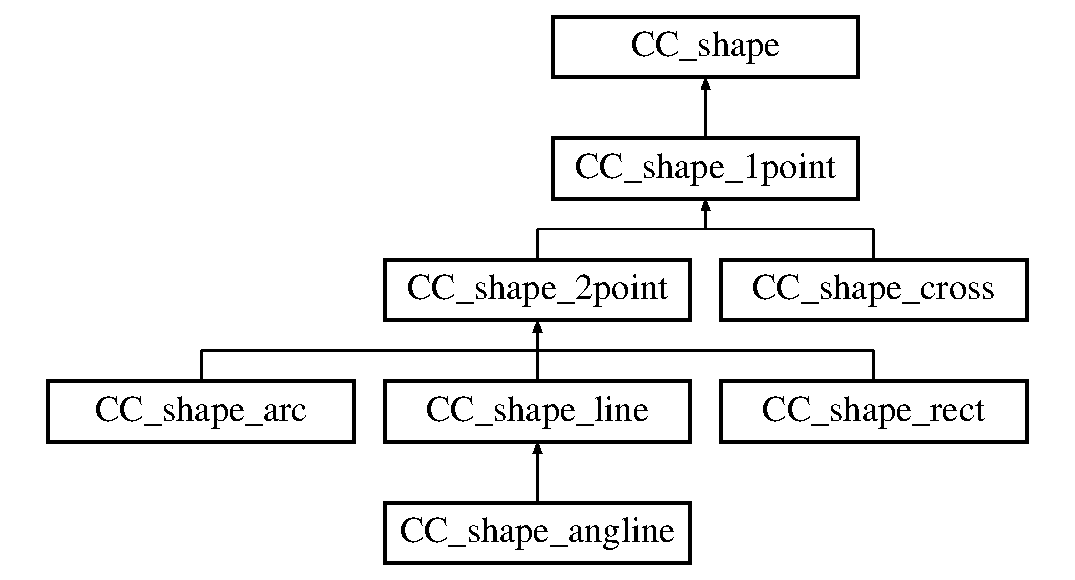
\includegraphics[height=5.000000cm]{a00038}
\end{center}
\end{figure}
\subsection*{Public Member Functions}
\begin{DoxyCompactItemize}
\item 
\hyperlink{a00038_a16f6e2d08cb21589759966bdc8827422}{C\-C\-\_\-shape\-\_\-1point} (const \hyperlink{a00029}{C\-C\-\_\-coord} \&p)
\item 
virtual void \hyperlink{a00038_a7110a3e16f7375074baa18efb997060a}{On\-Move} (const \hyperlink{a00029}{C\-C\-\_\-coord} \&p, const \hyperlink{a00029}{C\-C\-\_\-coord} \&snapped\-\_\-p)
\item 
void \hyperlink{a00038_a28d1b929bc908adb4530eb5a75b1bf56}{Move\-Origin} (const \hyperlink{a00029}{C\-C\-\_\-coord} \&p)
\item 
\hyperlink{a00029}{C\-C\-\_\-coord} \hyperlink{a00038_aa053b54300b73b01147d18a667fe8937}{Get\-Origin} () const 
\end{DoxyCompactItemize}
\subsection*{Protected Attributes}
\begin{DoxyCompactItemize}
\item 
\hyperlink{a00029}{C\-C\-\_\-coord} \hyperlink{a00038_a3e7c4e0c903b4331b98351cf8402b0cd}{origin}
\end{DoxyCompactItemize}


\subsection{Constructor \& Destructor Documentation}
\hypertarget{a00038_a16f6e2d08cb21589759966bdc8827422}{\index{C\-C\-\_\-shape\-\_\-1point@{C\-C\-\_\-shape\-\_\-1point}!C\-C\-\_\-shape\-\_\-1point@{C\-C\-\_\-shape\-\_\-1point}}
\index{C\-C\-\_\-shape\-\_\-1point@{C\-C\-\_\-shape\-\_\-1point}!CC_shape_1point@{C\-C\-\_\-shape\-\_\-1point}}
\subsubsection[{C\-C\-\_\-shape\-\_\-1point}]{\setlength{\rightskip}{0pt plus 5cm}C\-C\-\_\-shape\-\_\-1point\-::\-C\-C\-\_\-shape\-\_\-1point (
\begin{DoxyParamCaption}
\item[{const {\bf C\-C\-\_\-coord} \&}]{p}
\end{DoxyParamCaption}
)}}\label{a00038_a16f6e2d08cb21589759966bdc8827422}


\subsection{Member Function Documentation}
\hypertarget{a00038_aa053b54300b73b01147d18a667fe8937}{\index{C\-C\-\_\-shape\-\_\-1point@{C\-C\-\_\-shape\-\_\-1point}!Get\-Origin@{Get\-Origin}}
\index{Get\-Origin@{Get\-Origin}!CC_shape_1point@{C\-C\-\_\-shape\-\_\-1point}}
\subsubsection[{Get\-Origin}]{\setlength{\rightskip}{0pt plus 5cm}{\bf C\-C\-\_\-coord} C\-C\-\_\-shape\-\_\-1point\-::\-Get\-Origin (
\begin{DoxyParamCaption}
{}
\end{DoxyParamCaption}
) const}}\label{a00038_aa053b54300b73b01147d18a667fe8937}
\hypertarget{a00038_a28d1b929bc908adb4530eb5a75b1bf56}{\index{C\-C\-\_\-shape\-\_\-1point@{C\-C\-\_\-shape\-\_\-1point}!Move\-Origin@{Move\-Origin}}
\index{Move\-Origin@{Move\-Origin}!CC_shape_1point@{C\-C\-\_\-shape\-\_\-1point}}
\subsubsection[{Move\-Origin}]{\setlength{\rightskip}{0pt plus 5cm}void C\-C\-\_\-shape\-\_\-1point\-::\-Move\-Origin (
\begin{DoxyParamCaption}
\item[{const {\bf C\-C\-\_\-coord} \&}]{p}
\end{DoxyParamCaption}
)}}\label{a00038_a28d1b929bc908adb4530eb5a75b1bf56}
\hypertarget{a00038_a7110a3e16f7375074baa18efb997060a}{\index{C\-C\-\_\-shape\-\_\-1point@{C\-C\-\_\-shape\-\_\-1point}!On\-Move@{On\-Move}}
\index{On\-Move@{On\-Move}!CC_shape_1point@{C\-C\-\_\-shape\-\_\-1point}}
\subsubsection[{On\-Move}]{\setlength{\rightskip}{0pt plus 5cm}void C\-C\-\_\-shape\-\_\-1point\-::\-On\-Move (
\begin{DoxyParamCaption}
\item[{const {\bf C\-C\-\_\-coord} \&}]{p, }
\item[{const {\bf C\-C\-\_\-coord} \&}]{snapped\-\_\-p}
\end{DoxyParamCaption}
)\hspace{0.3cm}{\ttfamily [virtual]}}}\label{a00038_a7110a3e16f7375074baa18efb997060a}


Implements \hyperlink{a00037_a323c027fc21841c560b5759573b50f56}{C\-C\-\_\-shape}.



Reimplemented in \hyperlink{a00041_ac99e4b812a5eb489d29d324cd7dca7e5}{C\-C\-\_\-shape\-\_\-arc}, \hyperlink{a00040_a3aead16af5b691651d76d1d71138aae8}{C\-C\-\_\-shape\-\_\-angline}, \hyperlink{a00043_a8678d21e42e37bece16b3cac98241d98}{C\-C\-\_\-shape\-\_\-line}, \hyperlink{a00039_a5de0c111a1e2e01c7f2802333809b421}{C\-C\-\_\-shape\-\_\-2point}, and \hyperlink{a00042_a3326faef7625f5edfad2e5ba09927b6d}{C\-C\-\_\-shape\-\_\-cross}.



\subsection{Member Data Documentation}
\hypertarget{a00038_a3e7c4e0c903b4331b98351cf8402b0cd}{\index{C\-C\-\_\-shape\-\_\-1point@{C\-C\-\_\-shape\-\_\-1point}!origin@{origin}}
\index{origin@{origin}!CC_shape_1point@{C\-C\-\_\-shape\-\_\-1point}}
\subsubsection[{origin}]{\setlength{\rightskip}{0pt plus 5cm}{\bf C\-C\-\_\-coord} C\-C\-\_\-shape\-\_\-1point\-::origin\hspace{0.3cm}{\ttfamily [protected]}}}\label{a00038_a3e7c4e0c903b4331b98351cf8402b0cd}


The documentation for this class was generated from the following files\-:\begin{DoxyCompactItemize}
\item 
src/core/\hyperlink{a00210}{cc\-\_\-shapes.\-h}\item 
src/core/\hyperlink{a00209}{cc\-\_\-shapes.\-cpp}\end{DoxyCompactItemize}

\hypertarget{a00039}{\section{C\-C\-\_\-shape\-\_\-2point Class Reference}
\label{a00039}\index{C\-C\-\_\-shape\-\_\-2point@{C\-C\-\_\-shape\-\_\-2point}}
}


{\ttfamily \#include $<$cc\-\_\-shapes.\-h$>$}

Inheritance diagram for C\-C\-\_\-shape\-\_\-2point\-:\begin{figure}[H]
\begin{center}
\leavevmode
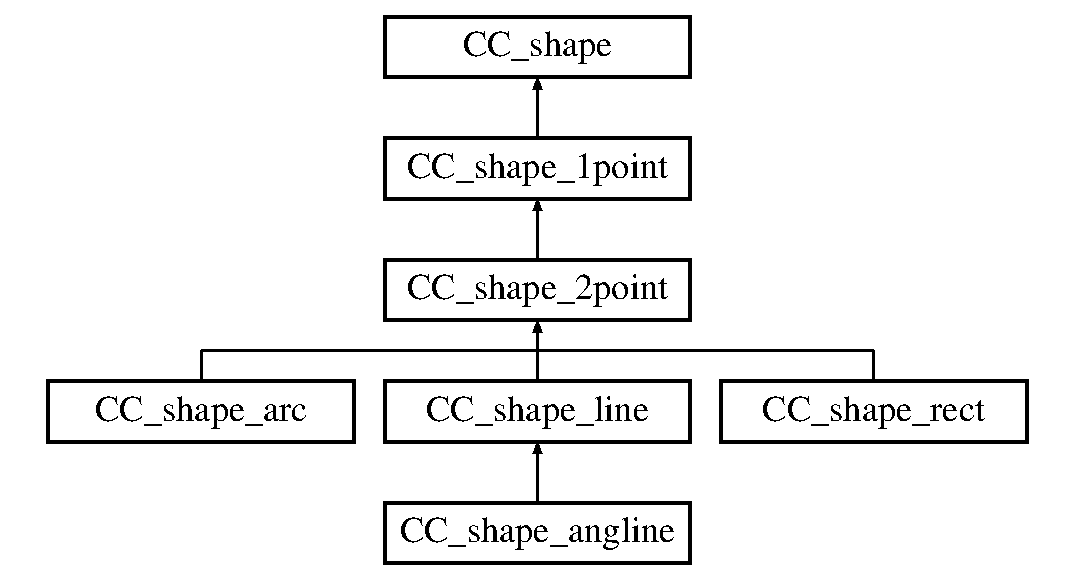
\includegraphics[height=5.000000cm]{a00039}
\end{center}
\end{figure}
\subsection*{Public Member Functions}
\begin{DoxyCompactItemize}
\item 
\hyperlink{a00039_a629fa854fbabd06dd41c1d0be1bbae5b}{C\-C\-\_\-shape\-\_\-2point} (const \hyperlink{a00029}{C\-C\-\_\-coord} \&p)
\item 
\hyperlink{a00039_afc6b4b2bbce2124f6d0ed30794e6bcf0}{C\-C\-\_\-shape\-\_\-2point} (const \hyperlink{a00029}{C\-C\-\_\-coord} \&p1, const \hyperlink{a00029}{C\-C\-\_\-coord} \&p2)
\item 
virtual void \hyperlink{a00039_a5de0c111a1e2e01c7f2802333809b421}{On\-Move} (const \hyperlink{a00029}{C\-C\-\_\-coord} \&p, const \hyperlink{a00029}{C\-C\-\_\-coord} \&snapped\-\_\-p)
\item 
void \hyperlink{a00039_a207d42c212c03ccae8e69918c52f5220}{Move\-Point} (const \hyperlink{a00029}{C\-C\-\_\-coord} \&p)
\item 
\hyperlink{a00029}{C\-C\-\_\-coord} \hyperlink{a00039_aa516703d68a080d1174c351d1ce6eb2c}{Get\-Point} () const 
\end{DoxyCompactItemize}
\subsection*{Protected Attributes}
\begin{DoxyCompactItemize}
\item 
\hyperlink{a00029}{C\-C\-\_\-coord} \hyperlink{a00039_acfded64430f596d55972e72349fabde7}{point}
\end{DoxyCompactItemize}


\subsection{Constructor \& Destructor Documentation}
\hypertarget{a00039_a629fa854fbabd06dd41c1d0be1bbae5b}{\index{C\-C\-\_\-shape\-\_\-2point@{C\-C\-\_\-shape\-\_\-2point}!C\-C\-\_\-shape\-\_\-2point@{C\-C\-\_\-shape\-\_\-2point}}
\index{C\-C\-\_\-shape\-\_\-2point@{C\-C\-\_\-shape\-\_\-2point}!CC_shape_2point@{C\-C\-\_\-shape\-\_\-2point}}
\subsubsection[{C\-C\-\_\-shape\-\_\-2point}]{\setlength{\rightskip}{0pt plus 5cm}C\-C\-\_\-shape\-\_\-2point\-::\-C\-C\-\_\-shape\-\_\-2point (
\begin{DoxyParamCaption}
\item[{const {\bf C\-C\-\_\-coord} \&}]{p}
\end{DoxyParamCaption}
)}}\label{a00039_a629fa854fbabd06dd41c1d0be1bbae5b}
\hypertarget{a00039_afc6b4b2bbce2124f6d0ed30794e6bcf0}{\index{C\-C\-\_\-shape\-\_\-2point@{C\-C\-\_\-shape\-\_\-2point}!C\-C\-\_\-shape\-\_\-2point@{C\-C\-\_\-shape\-\_\-2point}}
\index{C\-C\-\_\-shape\-\_\-2point@{C\-C\-\_\-shape\-\_\-2point}!CC_shape_2point@{C\-C\-\_\-shape\-\_\-2point}}
\subsubsection[{C\-C\-\_\-shape\-\_\-2point}]{\setlength{\rightskip}{0pt plus 5cm}C\-C\-\_\-shape\-\_\-2point\-::\-C\-C\-\_\-shape\-\_\-2point (
\begin{DoxyParamCaption}
\item[{const {\bf C\-C\-\_\-coord} \&}]{p1, }
\item[{const {\bf C\-C\-\_\-coord} \&}]{p2}
\end{DoxyParamCaption}
)}}\label{a00039_afc6b4b2bbce2124f6d0ed30794e6bcf0}


\subsection{Member Function Documentation}
\hypertarget{a00039_aa516703d68a080d1174c351d1ce6eb2c}{\index{C\-C\-\_\-shape\-\_\-2point@{C\-C\-\_\-shape\-\_\-2point}!Get\-Point@{Get\-Point}}
\index{Get\-Point@{Get\-Point}!CC_shape_2point@{C\-C\-\_\-shape\-\_\-2point}}
\subsubsection[{Get\-Point}]{\setlength{\rightskip}{0pt plus 5cm}{\bf C\-C\-\_\-coord} C\-C\-\_\-shape\-\_\-2point\-::\-Get\-Point (
\begin{DoxyParamCaption}
{}
\end{DoxyParamCaption}
) const}}\label{a00039_aa516703d68a080d1174c351d1ce6eb2c}
\hypertarget{a00039_a207d42c212c03ccae8e69918c52f5220}{\index{C\-C\-\_\-shape\-\_\-2point@{C\-C\-\_\-shape\-\_\-2point}!Move\-Point@{Move\-Point}}
\index{Move\-Point@{Move\-Point}!CC_shape_2point@{C\-C\-\_\-shape\-\_\-2point}}
\subsubsection[{Move\-Point}]{\setlength{\rightskip}{0pt plus 5cm}void C\-C\-\_\-shape\-\_\-2point\-::\-Move\-Point (
\begin{DoxyParamCaption}
\item[{const {\bf C\-C\-\_\-coord} \&}]{p}
\end{DoxyParamCaption}
)}}\label{a00039_a207d42c212c03ccae8e69918c52f5220}
\hypertarget{a00039_a5de0c111a1e2e01c7f2802333809b421}{\index{C\-C\-\_\-shape\-\_\-2point@{C\-C\-\_\-shape\-\_\-2point}!On\-Move@{On\-Move}}
\index{On\-Move@{On\-Move}!CC_shape_2point@{C\-C\-\_\-shape\-\_\-2point}}
\subsubsection[{On\-Move}]{\setlength{\rightskip}{0pt plus 5cm}void C\-C\-\_\-shape\-\_\-2point\-::\-On\-Move (
\begin{DoxyParamCaption}
\item[{const {\bf C\-C\-\_\-coord} \&}]{p, }
\item[{const {\bf C\-C\-\_\-coord} \&}]{snapped\-\_\-p}
\end{DoxyParamCaption}
)\hspace{0.3cm}{\ttfamily [virtual]}}}\label{a00039_a5de0c111a1e2e01c7f2802333809b421}


Reimplemented from \hyperlink{a00038_a7110a3e16f7375074baa18efb997060a}{C\-C\-\_\-shape\-\_\-1point}.



Reimplemented in \hyperlink{a00041_ac99e4b812a5eb489d29d324cd7dca7e5}{C\-C\-\_\-shape\-\_\-arc}, \hyperlink{a00040_a3aead16af5b691651d76d1d71138aae8}{C\-C\-\_\-shape\-\_\-angline}, and \hyperlink{a00043_a8678d21e42e37bece16b3cac98241d98}{C\-C\-\_\-shape\-\_\-line}.



\subsection{Member Data Documentation}
\hypertarget{a00039_acfded64430f596d55972e72349fabde7}{\index{C\-C\-\_\-shape\-\_\-2point@{C\-C\-\_\-shape\-\_\-2point}!point@{point}}
\index{point@{point}!CC_shape_2point@{C\-C\-\_\-shape\-\_\-2point}}
\subsubsection[{point}]{\setlength{\rightskip}{0pt plus 5cm}{\bf C\-C\-\_\-coord} C\-C\-\_\-shape\-\_\-2point\-::point\hspace{0.3cm}{\ttfamily [protected]}}}\label{a00039_acfded64430f596d55972e72349fabde7}


The documentation for this class was generated from the following files\-:\begin{DoxyCompactItemize}
\item 
src/core/\hyperlink{a00210}{cc\-\_\-shapes.\-h}\item 
src/core/\hyperlink{a00209}{cc\-\_\-shapes.\-cpp}\end{DoxyCompactItemize}

\hypertarget{a00040}{\section{C\-C\-\_\-shape\-\_\-angline Class Reference}
\label{a00040}\index{C\-C\-\_\-shape\-\_\-angline@{C\-C\-\_\-shape\-\_\-angline}}
}


{\ttfamily \#include $<$cc\-\_\-shapes.\-h$>$}

Inheritance diagram for C\-C\-\_\-shape\-\_\-angline\-:\begin{figure}[H]
\begin{center}
\leavevmode
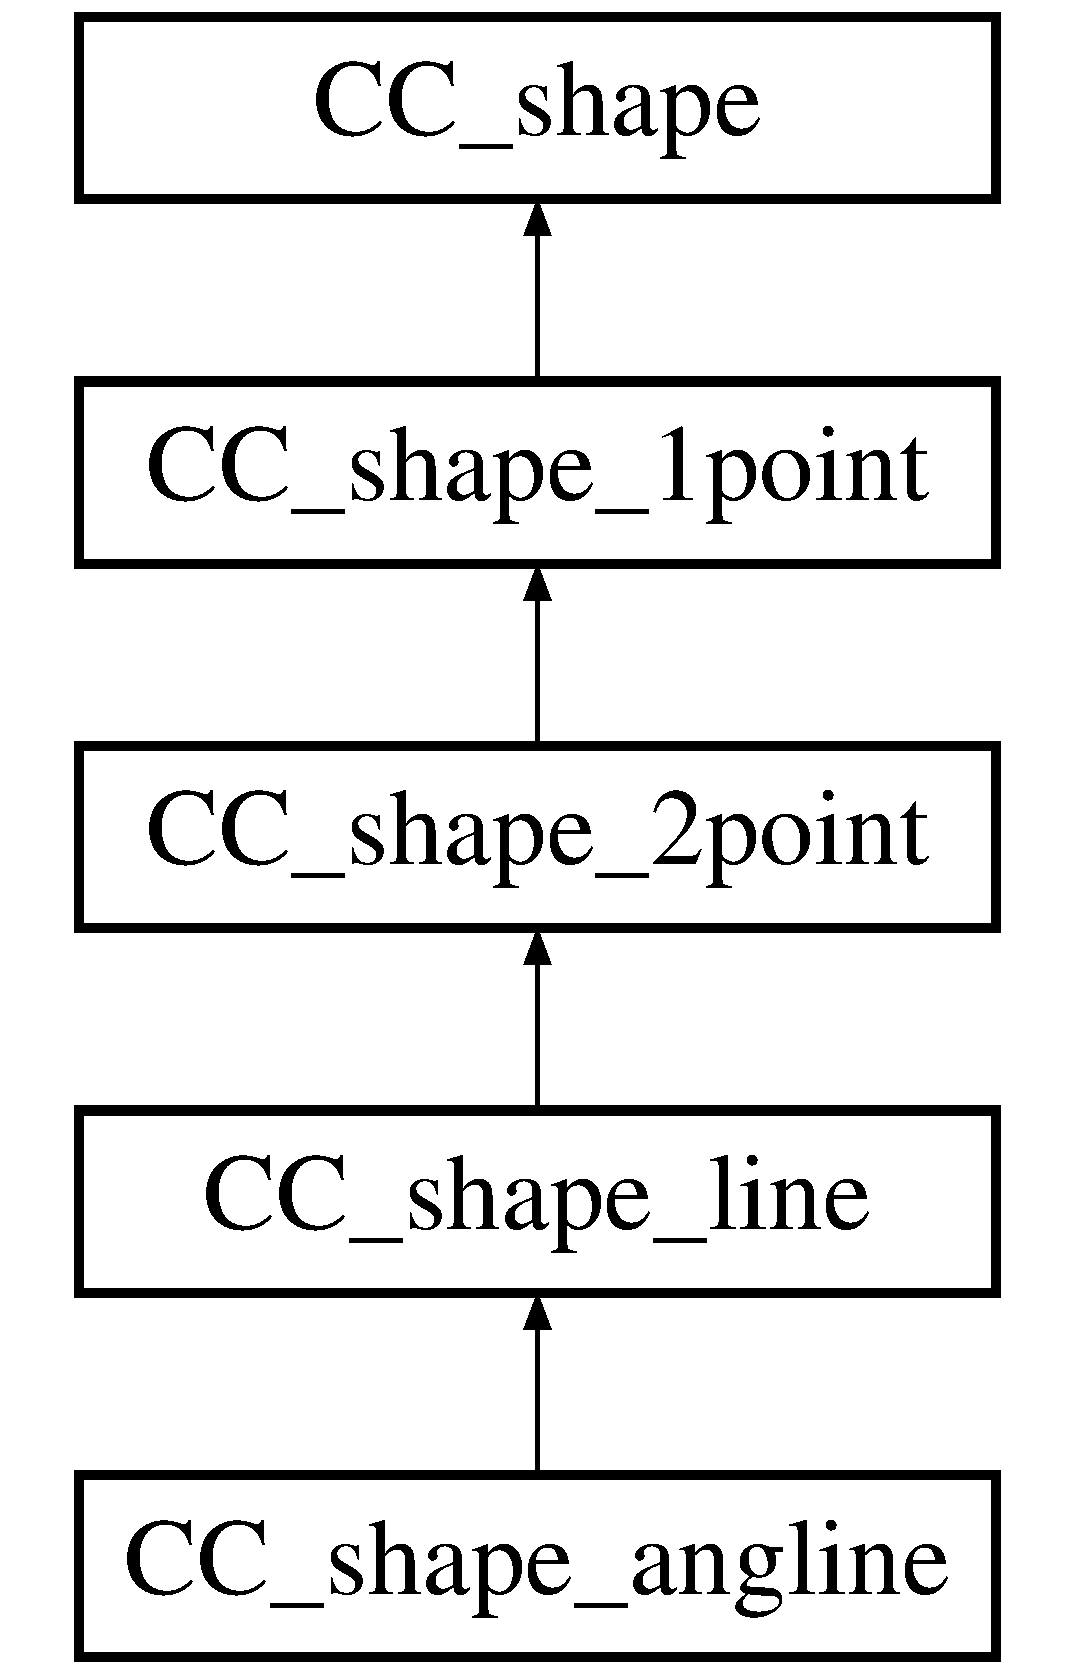
\includegraphics[height=5.000000cm]{a00040}
\end{center}
\end{figure}
\subsection*{Public Member Functions}
\begin{DoxyCompactItemize}
\item 
\hyperlink{a00040_a474bdcd7412ddbfa98c8d183e895a10d}{C\-C\-\_\-shape\-\_\-angline} (const \hyperlink{a00029}{C\-C\-\_\-coord} \&p, const \hyperlink{a00029}{C\-C\-\_\-coord} \&refvect)
\item 
virtual void \hyperlink{a00040_a3aead16af5b691651d76d1d71138aae8}{On\-Move} (const \hyperlink{a00029}{C\-C\-\_\-coord} \&p, const \hyperlink{a00029}{C\-C\-\_\-coord} \&snapped\-\_\-p)
\end{DoxyCompactItemize}
\subsection*{Private Attributes}
\begin{DoxyCompactItemize}
\item 
\hyperlink{a00029}{C\-C\-\_\-coord} \hyperlink{a00040_a19ab5a832d2fba6bbef2c0767da54f6c}{vect}
\item 
float \hyperlink{a00040_af6204d4bf9aadab09dc36e8a7f7c9bf2}{mag}
\end{DoxyCompactItemize}
\subsection*{Additional Inherited Members}


\subsection{Constructor \& Destructor Documentation}
\hypertarget{a00040_a474bdcd7412ddbfa98c8d183e895a10d}{\index{C\-C\-\_\-shape\-\_\-angline@{C\-C\-\_\-shape\-\_\-angline}!C\-C\-\_\-shape\-\_\-angline@{C\-C\-\_\-shape\-\_\-angline}}
\index{C\-C\-\_\-shape\-\_\-angline@{C\-C\-\_\-shape\-\_\-angline}!CC_shape_angline@{C\-C\-\_\-shape\-\_\-angline}}
\subsubsection[{C\-C\-\_\-shape\-\_\-angline}]{\setlength{\rightskip}{0pt plus 5cm}C\-C\-\_\-shape\-\_\-angline\-::\-C\-C\-\_\-shape\-\_\-angline (
\begin{DoxyParamCaption}
\item[{const {\bf C\-C\-\_\-coord} \&}]{p, }
\item[{const {\bf C\-C\-\_\-coord} \&}]{refvect}
\end{DoxyParamCaption}
)}}\label{a00040_a474bdcd7412ddbfa98c8d183e895a10d}


\subsection{Member Function Documentation}
\hypertarget{a00040_a3aead16af5b691651d76d1d71138aae8}{\index{C\-C\-\_\-shape\-\_\-angline@{C\-C\-\_\-shape\-\_\-angline}!On\-Move@{On\-Move}}
\index{On\-Move@{On\-Move}!CC_shape_angline@{C\-C\-\_\-shape\-\_\-angline}}
\subsubsection[{On\-Move}]{\setlength{\rightskip}{0pt plus 5cm}void C\-C\-\_\-shape\-\_\-angline\-::\-On\-Move (
\begin{DoxyParamCaption}
\item[{const {\bf C\-C\-\_\-coord} \&}]{p, }
\item[{const {\bf C\-C\-\_\-coord} \&}]{snapped\-\_\-p}
\end{DoxyParamCaption}
)\hspace{0.3cm}{\ttfamily [virtual]}}}\label{a00040_a3aead16af5b691651d76d1d71138aae8}


Reimplemented from \hyperlink{a00043_a8678d21e42e37bece16b3cac98241d98}{C\-C\-\_\-shape\-\_\-line}.



\subsection{Member Data Documentation}
\hypertarget{a00040_af6204d4bf9aadab09dc36e8a7f7c9bf2}{\index{C\-C\-\_\-shape\-\_\-angline@{C\-C\-\_\-shape\-\_\-angline}!mag@{mag}}
\index{mag@{mag}!CC_shape_angline@{C\-C\-\_\-shape\-\_\-angline}}
\subsubsection[{mag}]{\setlength{\rightskip}{0pt plus 5cm}float C\-C\-\_\-shape\-\_\-angline\-::mag\hspace{0.3cm}{\ttfamily [private]}}}\label{a00040_af6204d4bf9aadab09dc36e8a7f7c9bf2}
\hypertarget{a00040_a19ab5a832d2fba6bbef2c0767da54f6c}{\index{C\-C\-\_\-shape\-\_\-angline@{C\-C\-\_\-shape\-\_\-angline}!vect@{vect}}
\index{vect@{vect}!CC_shape_angline@{C\-C\-\_\-shape\-\_\-angline}}
\subsubsection[{vect}]{\setlength{\rightskip}{0pt plus 5cm}{\bf C\-C\-\_\-coord} C\-C\-\_\-shape\-\_\-angline\-::vect\hspace{0.3cm}{\ttfamily [private]}}}\label{a00040_a19ab5a832d2fba6bbef2c0767da54f6c}


The documentation for this class was generated from the following files\-:\begin{DoxyCompactItemize}
\item 
src/core/\hyperlink{a00210}{cc\-\_\-shapes.\-h}\item 
src/core/\hyperlink{a00209}{cc\-\_\-shapes.\-cpp}\end{DoxyCompactItemize}

\hypertarget{a00041}{\section{C\-C\-\_\-shape\-\_\-arc Class Reference}
\label{a00041}\index{C\-C\-\_\-shape\-\_\-arc@{C\-C\-\_\-shape\-\_\-arc}}
}


{\ttfamily \#include $<$cc\-\_\-shapes.\-h$>$}

Inheritance diagram for C\-C\-\_\-shape\-\_\-arc\-:\begin{figure}[H]
\begin{center}
\leavevmode
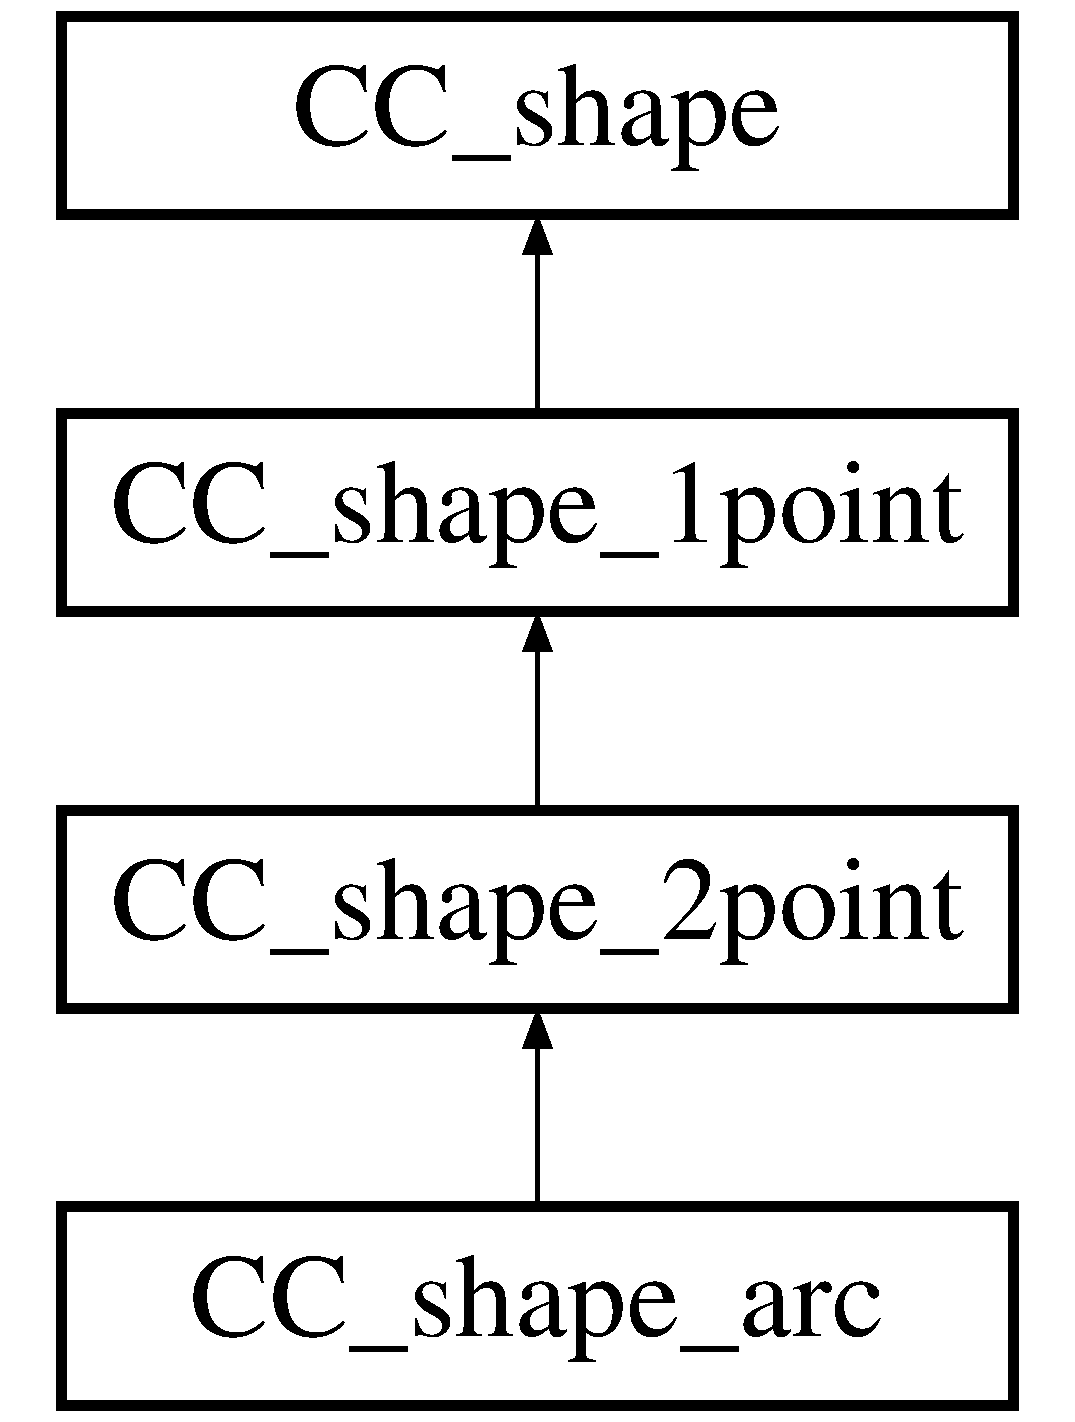
\includegraphics[height=4.000000cm]{a00041}
\end{center}
\end{figure}
\subsection*{Public Member Functions}
\begin{DoxyCompactItemize}
\item 
\hyperlink{a00041_a7ada4ea48bdb57dd83bca69412b8d65b}{C\-C\-\_\-shape\-\_\-arc} (const \hyperlink{a00029}{C\-C\-\_\-coord} \&c, const \hyperlink{a00029}{C\-C\-\_\-coord} \&p)
\item 
\hyperlink{a00041_a14e6776d9618db1f82e6214b6801a04e}{C\-C\-\_\-shape\-\_\-arc} (const \hyperlink{a00029}{C\-C\-\_\-coord} \&c, const \hyperlink{a00029}{C\-C\-\_\-coord} \&p1, const \hyperlink{a00029}{C\-C\-\_\-coord} \&p2)
\item 
virtual void \hyperlink{a00041_ac99e4b812a5eb489d29d324cd7dca7e5}{On\-Move} (const \hyperlink{a00029}{C\-C\-\_\-coord} \&p, const \hyperlink{a00029}{C\-C\-\_\-coord} \&snapped\-\_\-p)
\item 
virtual std\-::vector\\*
$<$ \hyperlink{a00031}{C\-C\-\_\-\-Draw\-Command} $>$ \hyperlink{a00041_aa8f4623a8093d5fb095912e2b13ccf80}{Get\-C\-C\-\_\-\-Draw\-Command} (float x, float y) const 
\item 
float \hyperlink{a00041_a822ebc83a7e441cb1b710f6599aad92b}{Get\-Angle} () const 
\end{DoxyCompactItemize}
\subsection*{Private Attributes}
\begin{DoxyCompactItemize}
\item 
float \hyperlink{a00041_a1046b77a88b111d22f31e1d07d9f1139}{r}
\item 
float \hyperlink{a00041_a4106c0d55812971a208ab527aeb516ac}{r0}
\item 
float \hyperlink{a00041_adc552191491a603591122b01970740d2}{d}
\end{DoxyCompactItemize}
\subsection*{Additional Inherited Members}


\subsection{Constructor \& Destructor Documentation}
\hypertarget{a00041_a7ada4ea48bdb57dd83bca69412b8d65b}{\index{C\-C\-\_\-shape\-\_\-arc@{C\-C\-\_\-shape\-\_\-arc}!C\-C\-\_\-shape\-\_\-arc@{C\-C\-\_\-shape\-\_\-arc}}
\index{C\-C\-\_\-shape\-\_\-arc@{C\-C\-\_\-shape\-\_\-arc}!CC_shape_arc@{C\-C\-\_\-shape\-\_\-arc}}
\subsubsection[{C\-C\-\_\-shape\-\_\-arc}]{\setlength{\rightskip}{0pt plus 5cm}C\-C\-\_\-shape\-\_\-arc\-::\-C\-C\-\_\-shape\-\_\-arc (
\begin{DoxyParamCaption}
\item[{const {\bf C\-C\-\_\-coord} \&}]{c, }
\item[{const {\bf C\-C\-\_\-coord} \&}]{p}
\end{DoxyParamCaption}
)}}\label{a00041_a7ada4ea48bdb57dd83bca69412b8d65b}
\hypertarget{a00041_a14e6776d9618db1f82e6214b6801a04e}{\index{C\-C\-\_\-shape\-\_\-arc@{C\-C\-\_\-shape\-\_\-arc}!C\-C\-\_\-shape\-\_\-arc@{C\-C\-\_\-shape\-\_\-arc}}
\index{C\-C\-\_\-shape\-\_\-arc@{C\-C\-\_\-shape\-\_\-arc}!CC_shape_arc@{C\-C\-\_\-shape\-\_\-arc}}
\subsubsection[{C\-C\-\_\-shape\-\_\-arc}]{\setlength{\rightskip}{0pt plus 5cm}C\-C\-\_\-shape\-\_\-arc\-::\-C\-C\-\_\-shape\-\_\-arc (
\begin{DoxyParamCaption}
\item[{const {\bf C\-C\-\_\-coord} \&}]{c, }
\item[{const {\bf C\-C\-\_\-coord} \&}]{p1, }
\item[{const {\bf C\-C\-\_\-coord} \&}]{p2}
\end{DoxyParamCaption}
)}}\label{a00041_a14e6776d9618db1f82e6214b6801a04e}


\subsection{Member Function Documentation}
\hypertarget{a00041_a822ebc83a7e441cb1b710f6599aad92b}{\index{C\-C\-\_\-shape\-\_\-arc@{C\-C\-\_\-shape\-\_\-arc}!Get\-Angle@{Get\-Angle}}
\index{Get\-Angle@{Get\-Angle}!CC_shape_arc@{C\-C\-\_\-shape\-\_\-arc}}
\subsubsection[{Get\-Angle}]{\setlength{\rightskip}{0pt plus 5cm}float C\-C\-\_\-shape\-\_\-arc\-::\-Get\-Angle (
\begin{DoxyParamCaption}
{}
\end{DoxyParamCaption}
) const\hspace{0.3cm}{\ttfamily [inline]}}}\label{a00041_a822ebc83a7e441cb1b710f6599aad92b}
\hypertarget{a00041_aa8f4623a8093d5fb095912e2b13ccf80}{\index{C\-C\-\_\-shape\-\_\-arc@{C\-C\-\_\-shape\-\_\-arc}!Get\-C\-C\-\_\-\-Draw\-Command@{Get\-C\-C\-\_\-\-Draw\-Command}}
\index{Get\-C\-C\-\_\-\-Draw\-Command@{Get\-C\-C\-\_\-\-Draw\-Command}!CC_shape_arc@{C\-C\-\_\-shape\-\_\-arc}}
\subsubsection[{Get\-C\-C\-\_\-\-Draw\-Command}]{\setlength{\rightskip}{0pt plus 5cm}std\-::vector$<$ {\bf C\-C\-\_\-\-Draw\-Command} $>$ C\-C\-\_\-shape\-\_\-arc\-::\-Get\-C\-C\-\_\-\-Draw\-Command (
\begin{DoxyParamCaption}
\item[{float}]{x, }
\item[{float}]{y}
\end{DoxyParamCaption}
) const\hspace{0.3cm}{\ttfamily [virtual]}}}\label{a00041_aa8f4623a8093d5fb095912e2b13ccf80}


Implements \hyperlink{a00037_aec026dc3fefc83bd03031e17307d073c}{C\-C\-\_\-shape}.

\hypertarget{a00041_ac99e4b812a5eb489d29d324cd7dca7e5}{\index{C\-C\-\_\-shape\-\_\-arc@{C\-C\-\_\-shape\-\_\-arc}!On\-Move@{On\-Move}}
\index{On\-Move@{On\-Move}!CC_shape_arc@{C\-C\-\_\-shape\-\_\-arc}}
\subsubsection[{On\-Move}]{\setlength{\rightskip}{0pt plus 5cm}void C\-C\-\_\-shape\-\_\-arc\-::\-On\-Move (
\begin{DoxyParamCaption}
\item[{const {\bf C\-C\-\_\-coord} \&}]{p, }
\item[{const {\bf C\-C\-\_\-coord} \&}]{snapped\-\_\-p}
\end{DoxyParamCaption}
)\hspace{0.3cm}{\ttfamily [virtual]}}}\label{a00041_ac99e4b812a5eb489d29d324cd7dca7e5}


Reimplemented from \hyperlink{a00039_a5de0c111a1e2e01c7f2802333809b421}{C\-C\-\_\-shape\-\_\-2point}.



\subsection{Member Data Documentation}
\hypertarget{a00041_adc552191491a603591122b01970740d2}{\index{C\-C\-\_\-shape\-\_\-arc@{C\-C\-\_\-shape\-\_\-arc}!d@{d}}
\index{d@{d}!CC_shape_arc@{C\-C\-\_\-shape\-\_\-arc}}
\subsubsection[{d}]{\setlength{\rightskip}{0pt plus 5cm}float C\-C\-\_\-shape\-\_\-arc\-::d\hspace{0.3cm}{\ttfamily [private]}}}\label{a00041_adc552191491a603591122b01970740d2}
\hypertarget{a00041_a1046b77a88b111d22f31e1d07d9f1139}{\index{C\-C\-\_\-shape\-\_\-arc@{C\-C\-\_\-shape\-\_\-arc}!r@{r}}
\index{r@{r}!CC_shape_arc@{C\-C\-\_\-shape\-\_\-arc}}
\subsubsection[{r}]{\setlength{\rightskip}{0pt plus 5cm}float C\-C\-\_\-shape\-\_\-arc\-::r\hspace{0.3cm}{\ttfamily [private]}}}\label{a00041_a1046b77a88b111d22f31e1d07d9f1139}
\hypertarget{a00041_a4106c0d55812971a208ab527aeb516ac}{\index{C\-C\-\_\-shape\-\_\-arc@{C\-C\-\_\-shape\-\_\-arc}!r0@{r0}}
\index{r0@{r0}!CC_shape_arc@{C\-C\-\_\-shape\-\_\-arc}}
\subsubsection[{r0}]{\setlength{\rightskip}{0pt plus 5cm}float C\-C\-\_\-shape\-\_\-arc\-::r0\hspace{0.3cm}{\ttfamily [private]}}}\label{a00041_a4106c0d55812971a208ab527aeb516ac}


The documentation for this class was generated from the following files\-:\begin{DoxyCompactItemize}
\item 
src/core/\hyperlink{a00210}{cc\-\_\-shapes.\-h}\item 
src/core/\hyperlink{a00209}{cc\-\_\-shapes.\-cpp}\end{DoxyCompactItemize}

\hypertarget{a00042}{\section{C\-C\-\_\-shape\-\_\-cross Class Reference}
\label{a00042}\index{C\-C\-\_\-shape\-\_\-cross@{C\-C\-\_\-shape\-\_\-cross}}
}


{\ttfamily \#include $<$cc\-\_\-shapes.\-h$>$}

Inheritance diagram for C\-C\-\_\-shape\-\_\-cross\-:\begin{figure}[H]
\begin{center}
\leavevmode
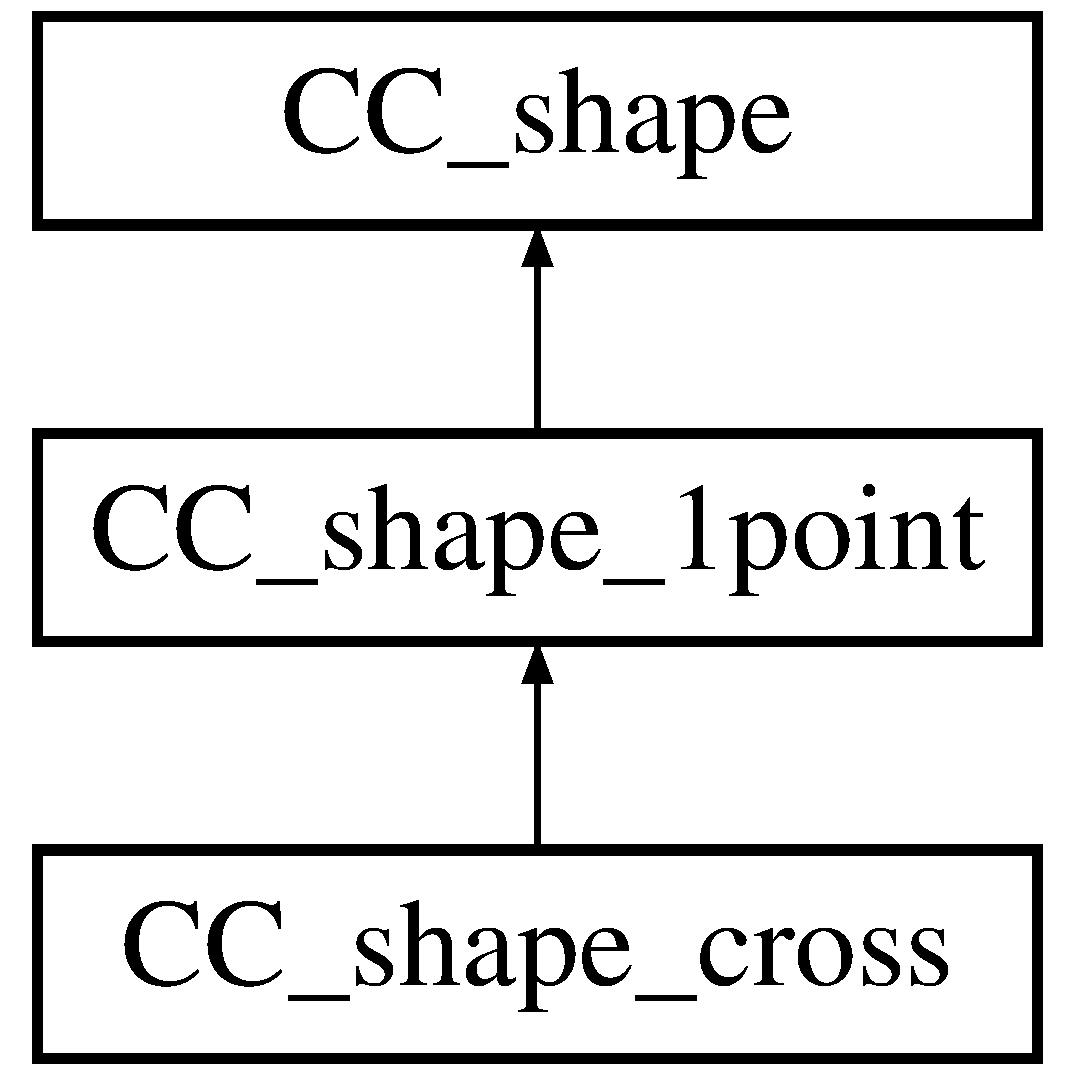
\includegraphics[height=3.000000cm]{a00042}
\end{center}
\end{figure}
\subsection*{Public Member Functions}
\begin{DoxyCompactItemize}
\item 
\hyperlink{a00042_a57daadb08b97a07f60da56af4b623cd1}{C\-C\-\_\-shape\-\_\-cross} (const \hyperlink{a00029}{C\-C\-\_\-coord} \&p, \hyperlink{a00216_acd9dae57b712df0e2d3588c0c4798c11}{Coord} width)
\item 
virtual void \hyperlink{a00042_a3326faef7625f5edfad2e5ba09927b6d}{On\-Move} (const \hyperlink{a00029}{C\-C\-\_\-coord} \&p, const \hyperlink{a00029}{C\-C\-\_\-coord} \&snapped\-\_\-p)
\item 
virtual std\-::vector\\*
$<$ \hyperlink{a00031}{C\-C\-\_\-\-Draw\-Command} $>$ \hyperlink{a00042_ad258d1e056279b8e1b37cc25ac286ed8}{Get\-C\-C\-\_\-\-Draw\-Command} (float x, float y) const 
\end{DoxyCompactItemize}
\subsection*{Protected Attributes}
\begin{DoxyCompactItemize}
\item 
\hyperlink{a00216_acd9dae57b712df0e2d3588c0c4798c11}{Coord} \hyperlink{a00042_a8e702535e5089fed5c19c2c7bb20d74f}{cross\-\_\-width}
\end{DoxyCompactItemize}


\subsection{Constructor \& Destructor Documentation}
\hypertarget{a00042_a57daadb08b97a07f60da56af4b623cd1}{\index{C\-C\-\_\-shape\-\_\-cross@{C\-C\-\_\-shape\-\_\-cross}!C\-C\-\_\-shape\-\_\-cross@{C\-C\-\_\-shape\-\_\-cross}}
\index{C\-C\-\_\-shape\-\_\-cross@{C\-C\-\_\-shape\-\_\-cross}!CC_shape_cross@{C\-C\-\_\-shape\-\_\-cross}}
\subsubsection[{C\-C\-\_\-shape\-\_\-cross}]{\setlength{\rightskip}{0pt plus 5cm}C\-C\-\_\-shape\-\_\-cross\-::\-C\-C\-\_\-shape\-\_\-cross (
\begin{DoxyParamCaption}
\item[{const {\bf C\-C\-\_\-coord} \&}]{p, }
\item[{{\bf Coord}}]{width}
\end{DoxyParamCaption}
)}}\label{a00042_a57daadb08b97a07f60da56af4b623cd1}


\subsection{Member Function Documentation}
\hypertarget{a00042_ad258d1e056279b8e1b37cc25ac286ed8}{\index{C\-C\-\_\-shape\-\_\-cross@{C\-C\-\_\-shape\-\_\-cross}!Get\-C\-C\-\_\-\-Draw\-Command@{Get\-C\-C\-\_\-\-Draw\-Command}}
\index{Get\-C\-C\-\_\-\-Draw\-Command@{Get\-C\-C\-\_\-\-Draw\-Command}!CC_shape_cross@{C\-C\-\_\-shape\-\_\-cross}}
\subsubsection[{Get\-C\-C\-\_\-\-Draw\-Command}]{\setlength{\rightskip}{0pt plus 5cm}std\-::vector$<$ {\bf C\-C\-\_\-\-Draw\-Command} $>$ C\-C\-\_\-shape\-\_\-cross\-::\-Get\-C\-C\-\_\-\-Draw\-Command (
\begin{DoxyParamCaption}
\item[{float}]{x, }
\item[{float}]{y}
\end{DoxyParamCaption}
) const\hspace{0.3cm}{\ttfamily [virtual]}}}\label{a00042_ad258d1e056279b8e1b37cc25ac286ed8}


Implements \hyperlink{a00037_aec026dc3fefc83bd03031e17307d073c}{C\-C\-\_\-shape}.

\hypertarget{a00042_a3326faef7625f5edfad2e5ba09927b6d}{\index{C\-C\-\_\-shape\-\_\-cross@{C\-C\-\_\-shape\-\_\-cross}!On\-Move@{On\-Move}}
\index{On\-Move@{On\-Move}!CC_shape_cross@{C\-C\-\_\-shape\-\_\-cross}}
\subsubsection[{On\-Move}]{\setlength{\rightskip}{0pt plus 5cm}void C\-C\-\_\-shape\-\_\-cross\-::\-On\-Move (
\begin{DoxyParamCaption}
\item[{const {\bf C\-C\-\_\-coord} \&}]{p, }
\item[{const {\bf C\-C\-\_\-coord} \&}]{snapped\-\_\-p}
\end{DoxyParamCaption}
)\hspace{0.3cm}{\ttfamily [virtual]}}}\label{a00042_a3326faef7625f5edfad2e5ba09927b6d}


Reimplemented from \hyperlink{a00038_a7110a3e16f7375074baa18efb997060a}{C\-C\-\_\-shape\-\_\-1point}.



\subsection{Member Data Documentation}
\hypertarget{a00042_a8e702535e5089fed5c19c2c7bb20d74f}{\index{C\-C\-\_\-shape\-\_\-cross@{C\-C\-\_\-shape\-\_\-cross}!cross\-\_\-width@{cross\-\_\-width}}
\index{cross\-\_\-width@{cross\-\_\-width}!CC_shape_cross@{C\-C\-\_\-shape\-\_\-cross}}
\subsubsection[{cross\-\_\-width}]{\setlength{\rightskip}{0pt plus 5cm}{\bf Coord} C\-C\-\_\-shape\-\_\-cross\-::cross\-\_\-width\hspace{0.3cm}{\ttfamily [protected]}}}\label{a00042_a8e702535e5089fed5c19c2c7bb20d74f}


The documentation for this class was generated from the following files\-:\begin{DoxyCompactItemize}
\item 
src/core/\hyperlink{a00210}{cc\-\_\-shapes.\-h}\item 
src/core/\hyperlink{a00209}{cc\-\_\-shapes.\-cpp}\end{DoxyCompactItemize}

\hypertarget{a00043}{\section{C\-C\-\_\-shape\-\_\-line Class Reference}
\label{a00043}\index{C\-C\-\_\-shape\-\_\-line@{C\-C\-\_\-shape\-\_\-line}}
}


{\ttfamily \#include $<$cc\-\_\-shapes.\-h$>$}

Inheritance diagram for C\-C\-\_\-shape\-\_\-line\-:\begin{figure}[H]
\begin{center}
\leavevmode
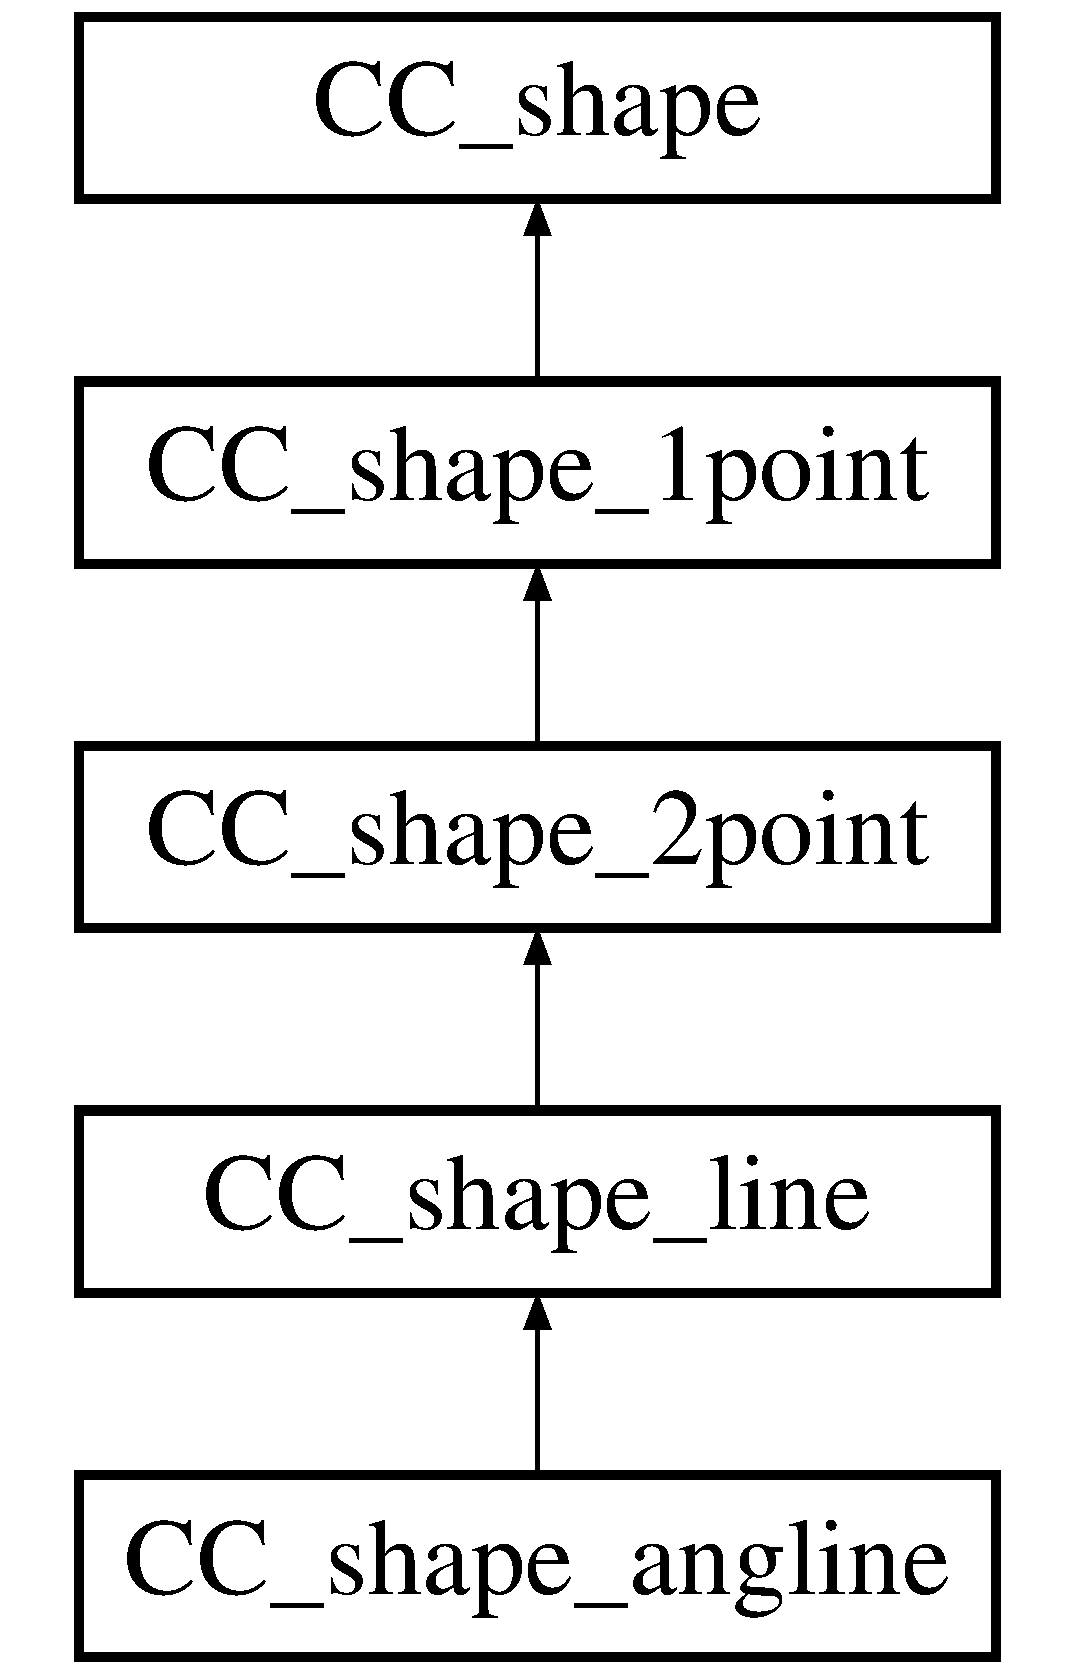
\includegraphics[height=5.000000cm]{a00043}
\end{center}
\end{figure}
\subsection*{Public Member Functions}
\begin{DoxyCompactItemize}
\item 
\hyperlink{a00043_abc7f311d22401f912cfae931aab7ef55}{C\-C\-\_\-shape\-\_\-line} (const \hyperlink{a00029}{C\-C\-\_\-coord} \&p)
\item 
\hyperlink{a00043_ab7a91b050e1d04206ad02279e0c58456}{C\-C\-\_\-shape\-\_\-line} (const \hyperlink{a00029}{C\-C\-\_\-coord} \&p1, const \hyperlink{a00029}{C\-C\-\_\-coord} \&p2)
\item 
virtual void \hyperlink{a00043_a8678d21e42e37bece16b3cac98241d98}{On\-Move} (const \hyperlink{a00029}{C\-C\-\_\-coord} \&p, const \hyperlink{a00029}{C\-C\-\_\-coord} \&snapped\-\_\-p)
\item 
virtual std\-::vector\\*
$<$ \hyperlink{a00031}{C\-C\-\_\-\-Draw\-Command} $>$ \hyperlink{a00043_a65124c0a0a223f45eb151b78c6f38ade}{Get\-C\-C\-\_\-\-Draw\-Command} (float x, float y) const 
\end{DoxyCompactItemize}
\subsection*{Additional Inherited Members}


\subsection{Constructor \& Destructor Documentation}
\hypertarget{a00043_abc7f311d22401f912cfae931aab7ef55}{\index{C\-C\-\_\-shape\-\_\-line@{C\-C\-\_\-shape\-\_\-line}!C\-C\-\_\-shape\-\_\-line@{C\-C\-\_\-shape\-\_\-line}}
\index{C\-C\-\_\-shape\-\_\-line@{C\-C\-\_\-shape\-\_\-line}!CC_shape_line@{C\-C\-\_\-shape\-\_\-line}}
\subsubsection[{C\-C\-\_\-shape\-\_\-line}]{\setlength{\rightskip}{0pt plus 5cm}C\-C\-\_\-shape\-\_\-line\-::\-C\-C\-\_\-shape\-\_\-line (
\begin{DoxyParamCaption}
\item[{const {\bf C\-C\-\_\-coord} \&}]{p}
\end{DoxyParamCaption}
)}}\label{a00043_abc7f311d22401f912cfae931aab7ef55}
\hypertarget{a00043_ab7a91b050e1d04206ad02279e0c58456}{\index{C\-C\-\_\-shape\-\_\-line@{C\-C\-\_\-shape\-\_\-line}!C\-C\-\_\-shape\-\_\-line@{C\-C\-\_\-shape\-\_\-line}}
\index{C\-C\-\_\-shape\-\_\-line@{C\-C\-\_\-shape\-\_\-line}!CC_shape_line@{C\-C\-\_\-shape\-\_\-line}}
\subsubsection[{C\-C\-\_\-shape\-\_\-line}]{\setlength{\rightskip}{0pt plus 5cm}C\-C\-\_\-shape\-\_\-line\-::\-C\-C\-\_\-shape\-\_\-line (
\begin{DoxyParamCaption}
\item[{const {\bf C\-C\-\_\-coord} \&}]{p1, }
\item[{const {\bf C\-C\-\_\-coord} \&}]{p2}
\end{DoxyParamCaption}
)}}\label{a00043_ab7a91b050e1d04206ad02279e0c58456}


\subsection{Member Function Documentation}
\hypertarget{a00043_a65124c0a0a223f45eb151b78c6f38ade}{\index{C\-C\-\_\-shape\-\_\-line@{C\-C\-\_\-shape\-\_\-line}!Get\-C\-C\-\_\-\-Draw\-Command@{Get\-C\-C\-\_\-\-Draw\-Command}}
\index{Get\-C\-C\-\_\-\-Draw\-Command@{Get\-C\-C\-\_\-\-Draw\-Command}!CC_shape_line@{C\-C\-\_\-shape\-\_\-line}}
\subsubsection[{Get\-C\-C\-\_\-\-Draw\-Command}]{\setlength{\rightskip}{0pt plus 5cm}std\-::vector$<$ {\bf C\-C\-\_\-\-Draw\-Command} $>$ C\-C\-\_\-shape\-\_\-line\-::\-Get\-C\-C\-\_\-\-Draw\-Command (
\begin{DoxyParamCaption}
\item[{float}]{x, }
\item[{float}]{y}
\end{DoxyParamCaption}
) const\hspace{0.3cm}{\ttfamily [virtual]}}}\label{a00043_a65124c0a0a223f45eb151b78c6f38ade}


Implements \hyperlink{a00037_aec026dc3fefc83bd03031e17307d073c}{C\-C\-\_\-shape}.

\hypertarget{a00043_a8678d21e42e37bece16b3cac98241d98}{\index{C\-C\-\_\-shape\-\_\-line@{C\-C\-\_\-shape\-\_\-line}!On\-Move@{On\-Move}}
\index{On\-Move@{On\-Move}!CC_shape_line@{C\-C\-\_\-shape\-\_\-line}}
\subsubsection[{On\-Move}]{\setlength{\rightskip}{0pt plus 5cm}void C\-C\-\_\-shape\-\_\-line\-::\-On\-Move (
\begin{DoxyParamCaption}
\item[{const {\bf C\-C\-\_\-coord} \&}]{p, }
\item[{const {\bf C\-C\-\_\-coord} \&}]{snapped\-\_\-p}
\end{DoxyParamCaption}
)\hspace{0.3cm}{\ttfamily [virtual]}}}\label{a00043_a8678d21e42e37bece16b3cac98241d98}


Reimplemented from \hyperlink{a00039_a5de0c111a1e2e01c7f2802333809b421}{C\-C\-\_\-shape\-\_\-2point}.



Reimplemented in \hyperlink{a00040_a3aead16af5b691651d76d1d71138aae8}{C\-C\-\_\-shape\-\_\-angline}.



The documentation for this class was generated from the following files\-:\begin{DoxyCompactItemize}
\item 
src/core/\hyperlink{a00210}{cc\-\_\-shapes.\-h}\item 
src/core/\hyperlink{a00209}{cc\-\_\-shapes.\-cpp}\end{DoxyCompactItemize}

\hypertarget{a00044}{\section{C\-C\-\_\-shape\-\_\-rect Class Reference}
\label{a00044}\index{C\-C\-\_\-shape\-\_\-rect@{C\-C\-\_\-shape\-\_\-rect}}
}


{\ttfamily \#include $<$cc\-\_\-shapes.\-h$>$}

Inheritance diagram for C\-C\-\_\-shape\-\_\-rect\-:\begin{figure}[H]
\begin{center}
\leavevmode
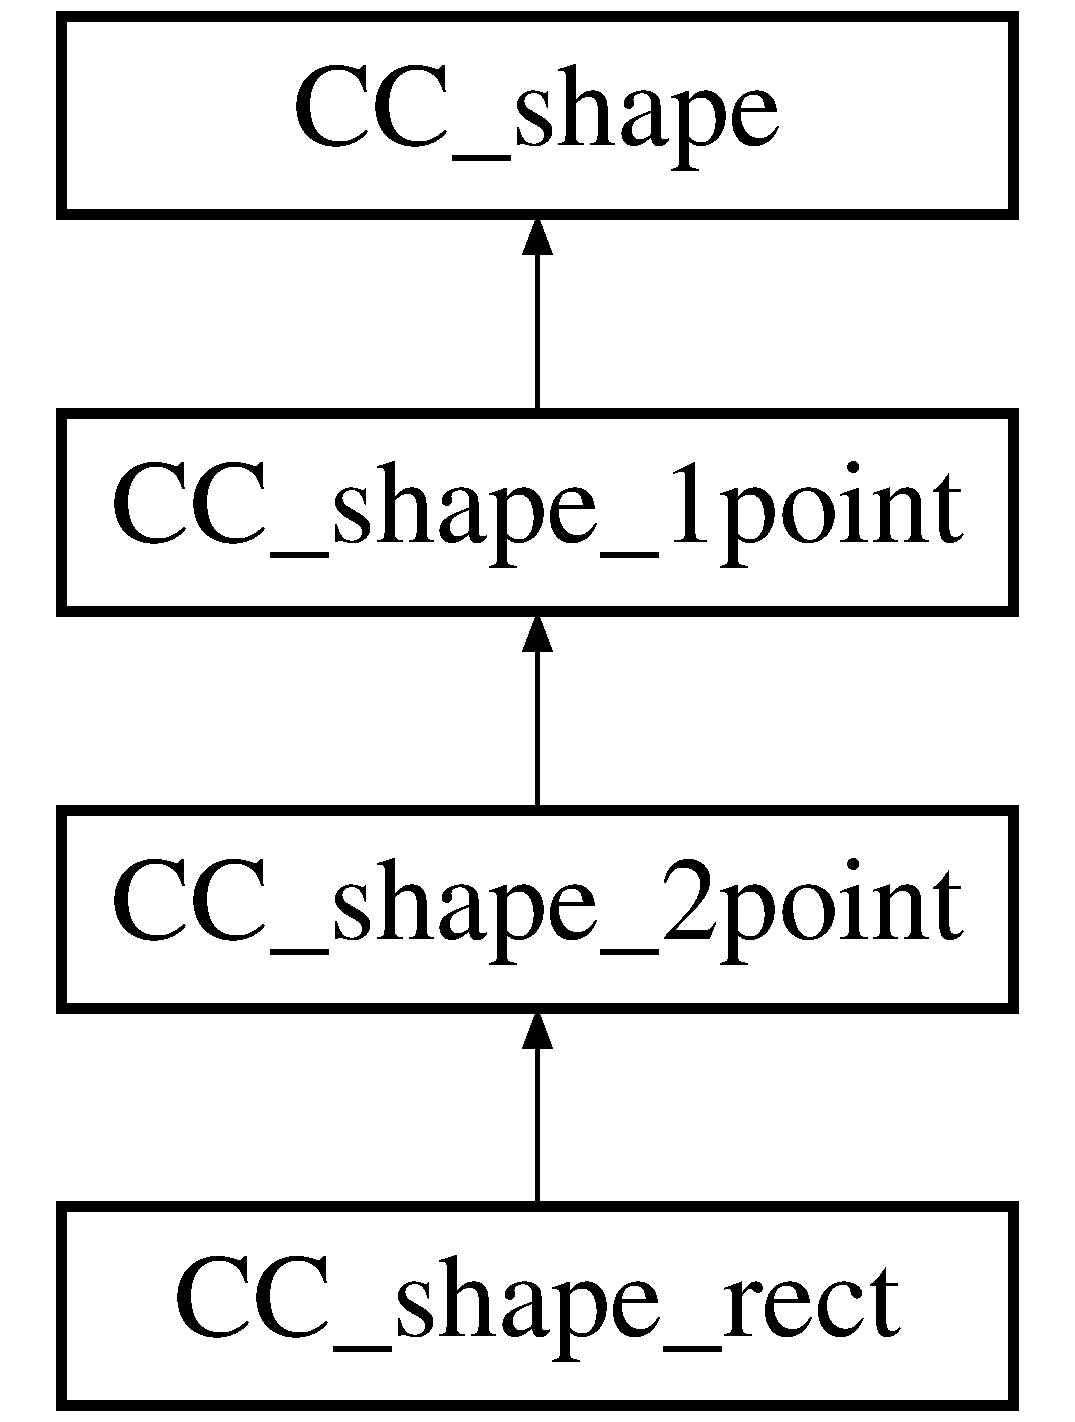
\includegraphics[height=4.000000cm]{a00044}
\end{center}
\end{figure}
\subsection*{Public Member Functions}
\begin{DoxyCompactItemize}
\item 
\hyperlink{a00044_af9b84c1d79e5fbe35cd14cc767978878}{C\-C\-\_\-shape\-\_\-rect} (const \hyperlink{a00029}{C\-C\-\_\-coord} \&p)
\item 
\hyperlink{a00044_a85eb247e35de03b622d4787a264be252}{C\-C\-\_\-shape\-\_\-rect} (const \hyperlink{a00029}{C\-C\-\_\-coord} \&p1, const \hyperlink{a00029}{C\-C\-\_\-coord} \&p2)
\item 
virtual std\-::vector\\*
$<$ \hyperlink{a00031}{C\-C\-\_\-\-Draw\-Command} $>$ \hyperlink{a00044_aca56590bb687ba94ce96b0c0e66116f7}{Get\-C\-C\-\_\-\-Draw\-Command} (float x, float y) const 
\end{DoxyCompactItemize}
\subsection*{Additional Inherited Members}


\subsection{Constructor \& Destructor Documentation}
\hypertarget{a00044_af9b84c1d79e5fbe35cd14cc767978878}{\index{C\-C\-\_\-shape\-\_\-rect@{C\-C\-\_\-shape\-\_\-rect}!C\-C\-\_\-shape\-\_\-rect@{C\-C\-\_\-shape\-\_\-rect}}
\index{C\-C\-\_\-shape\-\_\-rect@{C\-C\-\_\-shape\-\_\-rect}!CC_shape_rect@{C\-C\-\_\-shape\-\_\-rect}}
\subsubsection[{C\-C\-\_\-shape\-\_\-rect}]{\setlength{\rightskip}{0pt plus 5cm}C\-C\-\_\-shape\-\_\-rect\-::\-C\-C\-\_\-shape\-\_\-rect (
\begin{DoxyParamCaption}
\item[{const {\bf C\-C\-\_\-coord} \&}]{p}
\end{DoxyParamCaption}
)}}\label{a00044_af9b84c1d79e5fbe35cd14cc767978878}
\hypertarget{a00044_a85eb247e35de03b622d4787a264be252}{\index{C\-C\-\_\-shape\-\_\-rect@{C\-C\-\_\-shape\-\_\-rect}!C\-C\-\_\-shape\-\_\-rect@{C\-C\-\_\-shape\-\_\-rect}}
\index{C\-C\-\_\-shape\-\_\-rect@{C\-C\-\_\-shape\-\_\-rect}!CC_shape_rect@{C\-C\-\_\-shape\-\_\-rect}}
\subsubsection[{C\-C\-\_\-shape\-\_\-rect}]{\setlength{\rightskip}{0pt plus 5cm}C\-C\-\_\-shape\-\_\-rect\-::\-C\-C\-\_\-shape\-\_\-rect (
\begin{DoxyParamCaption}
\item[{const {\bf C\-C\-\_\-coord} \&}]{p1, }
\item[{const {\bf C\-C\-\_\-coord} \&}]{p2}
\end{DoxyParamCaption}
)}}\label{a00044_a85eb247e35de03b622d4787a264be252}


\subsection{Member Function Documentation}
\hypertarget{a00044_aca56590bb687ba94ce96b0c0e66116f7}{\index{C\-C\-\_\-shape\-\_\-rect@{C\-C\-\_\-shape\-\_\-rect}!Get\-C\-C\-\_\-\-Draw\-Command@{Get\-C\-C\-\_\-\-Draw\-Command}}
\index{Get\-C\-C\-\_\-\-Draw\-Command@{Get\-C\-C\-\_\-\-Draw\-Command}!CC_shape_rect@{C\-C\-\_\-shape\-\_\-rect}}
\subsubsection[{Get\-C\-C\-\_\-\-Draw\-Command}]{\setlength{\rightskip}{0pt plus 5cm}std\-::vector$<$ {\bf C\-C\-\_\-\-Draw\-Command} $>$ C\-C\-\_\-shape\-\_\-rect\-::\-Get\-C\-C\-\_\-\-Draw\-Command (
\begin{DoxyParamCaption}
\item[{float}]{x, }
\item[{float}]{y}
\end{DoxyParamCaption}
) const\hspace{0.3cm}{\ttfamily [virtual]}}}\label{a00044_aca56590bb687ba94ce96b0c0e66116f7}


Implements \hyperlink{a00037_aec026dc3fefc83bd03031e17307d073c}{C\-C\-\_\-shape}.



The documentation for this class was generated from the following files\-:\begin{DoxyCompactItemize}
\item 
src/core/\hyperlink{a00210}{cc\-\_\-shapes.\-h}\item 
src/core/\hyperlink{a00209}{cc\-\_\-shapes.\-cpp}\end{DoxyCompactItemize}

\hypertarget{a00045}{\section{C\-C\-\_\-sheet Class Reference}
\label{a00045}\index{C\-C\-\_\-sheet@{C\-C\-\_\-sheet}}
}


\hyperlink{a00045}{C\-C\-\_\-sheet} is a class representing a stunt sheet in a Cal\-Chart show.  




{\ttfamily \#include $<$cc\-\_\-sheet.\-h$>$}

\subsection*{Public Member Functions}
\begin{DoxyCompactItemize}
\item 
\hyperlink{a00045_ab0c9904f0e686fbe57c6ca6bdba09bab}{C\-C\-\_\-sheet} (\hyperlink{a00046}{C\-C\-\_\-show} $\ast$shw)
\item 
\hyperlink{a00045_a30372414cfea18692e4dab3953f6a72c}{C\-C\-\_\-sheet} (\hyperlink{a00046}{C\-C\-\_\-show} $\ast$shw, size\-\_\-t num\-Points, std\-::istream \&stream, \hyperlink{a00153}{Version\-\_\-3\-\_\-3\-\_\-and\-\_\-earlier})
\item 
\hyperlink{a00045_acbccbd9050a2b2a1b4a4dc391669647f}{C\-C\-\_\-sheet} (\hyperlink{a00046}{C\-C\-\_\-show} $\ast$shw, size\-\_\-t num\-Points, std\-::istream \&stream, \hyperlink{a00097}{Current\-\_\-version\-\_\-and\-\_\-later})
\item 
\hyperlink{a00045_afa1de8d4ee5bbd666578eaaf6944578f}{C\-C\-\_\-sheet} (\hyperlink{a00046}{C\-C\-\_\-show} $\ast$shw, const std\-::string \&newname)
\item 
\hyperlink{a00045_ac6f9cf59f8311ccac9c2335c16711e2a}{$\sim$\-C\-C\-\_\-sheet} ()
\item 
std\-::vector$<$ uint8\-\_\-t $>$ \hyperlink{a00045_afc1de05de1b53f5f59ad47c310ed334f}{Serialize\-Sheet} () const 
\item 
const \hyperlink{a00027}{C\-C\-\_\-continuity} \& \hyperlink{a00045_a85deb4da787ce4624eae061d227efc50}{Get\-Continuity\-By\-Symbol} (\hyperlink{a00216_a68cd84e0300be6f9ff4474682762c9ee}{S\-Y\-M\-B\-O\-L\-\_\-\-T\-Y\-P\-E} i) const 
\item 
std\-::set$<$ unsigned $>$ \hyperlink{a00045_a35396e54a607e36b4f6a1f48cf34f94a}{Select\-Points\-By\-Symbol} (\hyperlink{a00216_a68cd84e0300be6f9ff4474682762c9ee}{S\-Y\-M\-B\-O\-L\-\_\-\-T\-Y\-P\-E} i) const 
\item 
bool \hyperlink{a00045_aa85fcbaf88cd05db8fd2ece3aa49b2a8}{Continuity\-In\-Use} (\hyperlink{a00216_a68cd84e0300be6f9ff4474682762c9ee}{S\-Y\-M\-B\-O\-L\-\_\-\-T\-Y\-P\-E} idx) const 
\item 
void \hyperlink{a00045_ac50742b3a8b670e324a510d936b62a85}{Set\-Num\-Points} (unsigned num, unsigned columns, const \hyperlink{a00029}{C\-C\-\_\-coord} \&new\-\_\-march\-\_\-position)
\item 
void \hyperlink{a00045_a72d0ca96ad22fe792ca2469195a27367}{Set\-Continuity\-Text} (\hyperlink{a00216_a68cd84e0300be6f9ff4474682762c9ee}{S\-Y\-M\-B\-O\-L\-\_\-\-T\-Y\-P\-E} sym, const std\-::string \&text)
\item 
int \hyperlink{a00045_a559857fc852c580f272ce53295b59023}{Find\-Point} (\hyperlink{a00216_acd9dae57b712df0e2d3588c0c4798c11}{Coord} x, \hyperlink{a00216_acd9dae57b712df0e2d3588c0c4798c11}{Coord} y, \hyperlink{a00216_acd9dae57b712df0e2d3588c0c4798c11}{Coord} search\-Bound, unsigned ref=0) const 
\item 
void \hyperlink{a00045_a13b5c778494626306264b05ab0e26648}{Relabel\-Sheet} (const std\-::vector$<$ size\-\_\-t $>$ \&table)
\item 
std\-::string \hyperlink{a00045_a8fd7bccd609d86f0df42f12055c32178}{Get\-Name} () const 
\item 
void \hyperlink{a00045_a4a6f9925779f8bf529d448a31c13d21c}{Set\-Name} (const std\-::string \&newname)
\item 
std\-::string \hyperlink{a00045_a8fd164675fb15825e1087abefbd2535d}{Get\-Number} () const 
\item 
void \hyperlink{a00045_a3da05d3a78f81a0131d4101302d6b1c7}{Set\-Number} (const std\-::string \&newnumber)
\item 
unsigned short \hyperlink{a00045_af804d3260ad50627f4b119ac1e070cec}{Get\-Beats} () const 
\item 
void \hyperlink{a00045_a0f6fe0c0cfcf494d7eb7ade61c45e31d}{Set\-Beats} (unsigned short b)
\item 
bool \hyperlink{a00045_a44cce522fb28d50d9950b55e43d977a0}{Is\-In\-Animation} () const 
\item 
const \hyperlink{a00034}{C\-C\-\_\-point} \& \hyperlink{a00045_a435211f11fa9b77df4b2c2a3a08d1c8f}{Get\-Point} (unsigned i) const 
\item 
\hyperlink{a00034}{C\-C\-\_\-point} \& \hyperlink{a00045_a34496eced95d937a56be551b12c7cc8c}{Get\-Point} (unsigned i)
\item 
std\-::vector$<$ \hyperlink{a00034}{C\-C\-\_\-point} $>$ \hyperlink{a00045_a3b9e00f0f832d38a87348f4034462f6d}{Get\-Points} () const 
\item 
void \hyperlink{a00045_ae553f706e9d0f5e4a21465b3d628e086}{Set\-Points} (const std\-::vector$<$ \hyperlink{a00034}{C\-C\-\_\-point} $>$ \&points)
\item 
\hyperlink{a00029}{C\-C\-\_\-coord} \hyperlink{a00045_acee5043c5298517ae6af21fa6d4bf418}{Get\-Position} (unsigned i, unsigned ref=0) const 
\item 
void \hyperlink{a00045_aae68e9352eaff311790b59470461886b}{Set\-All\-Positions} (const \hyperlink{a00029}{C\-C\-\_\-coord} \&val, unsigned i)
\item 
void \hyperlink{a00045_a37d4e6d9c5a8865e02292ceb40ae0a1f}{Set\-Position} (const \hyperlink{a00029}{C\-C\-\_\-coord} \&val, unsigned i, unsigned ref=0)
\item 
bool \hyperlink{a00045_a81ee7a43bdc2e9e4f119413d8c1cb575}{Import\-Printable\-Continuity} (const std\-::vector$<$ std\-::string $>$ \&lines)
\item 
\hyperlink{a00212_ae492d9b165445899a5c5a3128e58f0cf}{C\-C\-\_\-textline\-\_\-list} \hyperlink{a00045_aadb6eccd1efa0023c1d4504e38984682}{Get\-Printable\-Continuity} () const 
\end{DoxyCompactItemize}
\subsection*{Private Types}
\begin{DoxyCompactItemize}
\item 
typedef std\-::vector\\*
$<$ \hyperlink{a00027}{C\-C\-\_\-continuity} $>$ \hyperlink{a00045_a057981286a04d0a0bf0b7ecbdd5e1bcd}{Cont\-Container}
\end{DoxyCompactItemize}
\subsection*{Private Member Functions}
\begin{DoxyCompactItemize}
\item 
std\-::vector$<$ uint8\-\_\-t $>$ \hyperlink{a00045_a6167e427cbf4b3ddd6744238167802ae}{Serialize\-All\-Points} () const 
\item 
std\-::vector$<$ uint8\-\_\-t $>$ \hyperlink{a00045_aadf23b9bf05af20065bbbdeb21c58f1a}{Serialize\-Continuity\-Data} () const 
\item 
std\-::vector$<$ uint8\-\_\-t $>$ \hyperlink{a00045_a763578b37626d3f15494539a6e2c6739}{Serialize\-Sheet\-Data} () const 
\item 
\hyperlink{a00027}{C\-C\-\_\-continuity} \& \hyperlink{a00045_ac2b623ff7a5cd2c1f17c24979c56b41a}{Get\-Continuity\-By\-Symbol} (\hyperlink{a00216_a68cd84e0300be6f9ff4474682762c9ee}{S\-Y\-M\-B\-O\-L\-\_\-\-T\-Y\-P\-E} i)
\end{DoxyCompactItemize}
\subsection*{Private Attributes}
\begin{DoxyCompactItemize}
\item 
\hyperlink{a00045_a057981286a04d0a0bf0b7ecbdd5e1bcd}{Cont\-Container} \hyperlink{a00045_a48691d0c3f157765c1b6448e572f3e0e}{m\-Animation\-Continuity}
\item 
\hyperlink{a00212_ae492d9b165445899a5c5a3128e58f0cf}{C\-C\-\_\-textline\-\_\-list} \hyperlink{a00045_aa55d5937b4aa3bf410c598d0b73e937c}{m\-Printable\-Continuity}
\item 
unsigned short \hyperlink{a00045_ae0a4f2825ed321a631bd179ee97ce990}{beats}
\item 
std\-::vector$<$ \hyperlink{a00034}{C\-C\-\_\-point} $>$ \hyperlink{a00045_a518af96eb5163fccb757e5f1d23fef17}{pts}
\item 
std\-::string \hyperlink{a00045_a8eee8546bf15f01705734cddaf7e1866}{m\-Name}
\item 
std\-::string \hyperlink{a00045_a075899cc4758e99aa40c51005c2b6458}{number}
\end{DoxyCompactItemize}


\subsection{Detailed Description}
\hyperlink{a00045}{C\-C\-\_\-sheet} is a class representing a stunt sheet in a Cal\-Chart show. 

It 

\subsection{Member Typedef Documentation}
\hypertarget{a00045_a057981286a04d0a0bf0b7ecbdd5e1bcd}{\index{C\-C\-\_\-sheet@{C\-C\-\_\-sheet}!Cont\-Container@{Cont\-Container}}
\index{Cont\-Container@{Cont\-Container}!CC_sheet@{C\-C\-\_\-sheet}}
\subsubsection[{Cont\-Container}]{\setlength{\rightskip}{0pt plus 5cm}typedef std\-::vector$<${\bf C\-C\-\_\-continuity}$>$ {\bf C\-C\-\_\-sheet\-::\-Cont\-Container}\hspace{0.3cm}{\ttfamily [private]}}}\label{a00045_a057981286a04d0a0bf0b7ecbdd5e1bcd}


\subsection{Constructor \& Destructor Documentation}
\hypertarget{a00045_ab0c9904f0e686fbe57c6ca6bdba09bab}{\index{C\-C\-\_\-sheet@{C\-C\-\_\-sheet}!C\-C\-\_\-sheet@{C\-C\-\_\-sheet}}
\index{C\-C\-\_\-sheet@{C\-C\-\_\-sheet}!CC_sheet@{C\-C\-\_\-sheet}}
\subsubsection[{C\-C\-\_\-sheet}]{\setlength{\rightskip}{0pt plus 5cm}C\-C\-\_\-sheet\-::\-C\-C\-\_\-sheet (
\begin{DoxyParamCaption}
\item[{{\bf C\-C\-\_\-show} $\ast$}]{shw}
\end{DoxyParamCaption}
)}}\label{a00045_ab0c9904f0e686fbe57c6ca6bdba09bab}
\hypertarget{a00045_a30372414cfea18692e4dab3953f6a72c}{\index{C\-C\-\_\-sheet@{C\-C\-\_\-sheet}!C\-C\-\_\-sheet@{C\-C\-\_\-sheet}}
\index{C\-C\-\_\-sheet@{C\-C\-\_\-sheet}!CC_sheet@{C\-C\-\_\-sheet}}
\subsubsection[{C\-C\-\_\-sheet}]{\setlength{\rightskip}{0pt plus 5cm}C\-C\-\_\-sheet\-::\-C\-C\-\_\-sheet (
\begin{DoxyParamCaption}
\item[{{\bf C\-C\-\_\-show} $\ast$}]{shw, }
\item[{size\-\_\-t}]{num\-Points, }
\item[{std\-::istream \&}]{stream, }
\item[{{\bf Version\-\_\-3\-\_\-3\-\_\-and\-\_\-earlier}}]{}
\end{DoxyParamCaption}
)}}\label{a00045_a30372414cfea18692e4dab3953f6a72c}
\hypertarget{a00045_acbccbd9050a2b2a1b4a4dc391669647f}{\index{C\-C\-\_\-sheet@{C\-C\-\_\-sheet}!C\-C\-\_\-sheet@{C\-C\-\_\-sheet}}
\index{C\-C\-\_\-sheet@{C\-C\-\_\-sheet}!CC_sheet@{C\-C\-\_\-sheet}}
\subsubsection[{C\-C\-\_\-sheet}]{\setlength{\rightskip}{0pt plus 5cm}C\-C\-\_\-sheet\-::\-C\-C\-\_\-sheet (
\begin{DoxyParamCaption}
\item[{{\bf C\-C\-\_\-show} $\ast$}]{shw, }
\item[{size\-\_\-t}]{num\-Points, }
\item[{std\-::istream \&}]{stream, }
\item[{{\bf Current\-\_\-version\-\_\-and\-\_\-later}}]{}
\end{DoxyParamCaption}
)}}\label{a00045_acbccbd9050a2b2a1b4a4dc391669647f}
\hypertarget{a00045_afa1de8d4ee5bbd666578eaaf6944578f}{\index{C\-C\-\_\-sheet@{C\-C\-\_\-sheet}!C\-C\-\_\-sheet@{C\-C\-\_\-sheet}}
\index{C\-C\-\_\-sheet@{C\-C\-\_\-sheet}!CC_sheet@{C\-C\-\_\-sheet}}
\subsubsection[{C\-C\-\_\-sheet}]{\setlength{\rightskip}{0pt plus 5cm}C\-C\-\_\-sheet\-::\-C\-C\-\_\-sheet (
\begin{DoxyParamCaption}
\item[{{\bf C\-C\-\_\-show} $\ast$}]{shw, }
\item[{const std\-::string \&}]{newname}
\end{DoxyParamCaption}
)}}\label{a00045_afa1de8d4ee5bbd666578eaaf6944578f}
\hypertarget{a00045_ac6f9cf59f8311ccac9c2335c16711e2a}{\index{C\-C\-\_\-sheet@{C\-C\-\_\-sheet}!$\sim$\-C\-C\-\_\-sheet@{$\sim$\-C\-C\-\_\-sheet}}
\index{$\sim$\-C\-C\-\_\-sheet@{$\sim$\-C\-C\-\_\-sheet}!CC_sheet@{C\-C\-\_\-sheet}}
\subsubsection[{$\sim$\-C\-C\-\_\-sheet}]{\setlength{\rightskip}{0pt plus 5cm}C\-C\-\_\-sheet\-::$\sim$\-C\-C\-\_\-sheet (
\begin{DoxyParamCaption}
{}
\end{DoxyParamCaption}
)}}\label{a00045_ac6f9cf59f8311ccac9c2335c16711e2a}


\subsection{Member Function Documentation}
\hypertarget{a00045_aa85fcbaf88cd05db8fd2ece3aa49b2a8}{\index{C\-C\-\_\-sheet@{C\-C\-\_\-sheet}!Continuity\-In\-Use@{Continuity\-In\-Use}}
\index{Continuity\-In\-Use@{Continuity\-In\-Use}!CC_sheet@{C\-C\-\_\-sheet}}
\subsubsection[{Continuity\-In\-Use}]{\setlength{\rightskip}{0pt plus 5cm}bool C\-C\-\_\-sheet\-::\-Continuity\-In\-Use (
\begin{DoxyParamCaption}
\item[{{\bf S\-Y\-M\-B\-O\-L\-\_\-\-T\-Y\-P\-E}}]{idx}
\end{DoxyParamCaption}
) const}}\label{a00045_aa85fcbaf88cd05db8fd2ece3aa49b2a8}
\hypertarget{a00045_a559857fc852c580f272ce53295b59023}{\index{C\-C\-\_\-sheet@{C\-C\-\_\-sheet}!Find\-Point@{Find\-Point}}
\index{Find\-Point@{Find\-Point}!CC_sheet@{C\-C\-\_\-sheet}}
\subsubsection[{Find\-Point}]{\setlength{\rightskip}{0pt plus 5cm}int C\-C\-\_\-sheet\-::\-Find\-Point (
\begin{DoxyParamCaption}
\item[{{\bf Coord}}]{x, }
\item[{{\bf Coord}}]{y, }
\item[{{\bf Coord}}]{search\-Bound, }
\item[{unsigned}]{ref = {\ttfamily 0}}
\end{DoxyParamCaption}
) const}}\label{a00045_a559857fc852c580f272ce53295b59023}
\hypertarget{a00045_af804d3260ad50627f4b119ac1e070cec}{\index{C\-C\-\_\-sheet@{C\-C\-\_\-sheet}!Get\-Beats@{Get\-Beats}}
\index{Get\-Beats@{Get\-Beats}!CC_sheet@{C\-C\-\_\-sheet}}
\subsubsection[{Get\-Beats}]{\setlength{\rightskip}{0pt plus 5cm}unsigned short C\-C\-\_\-sheet\-::\-Get\-Beats (
\begin{DoxyParamCaption}
{}
\end{DoxyParamCaption}
) const}}\label{a00045_af804d3260ad50627f4b119ac1e070cec}
\hypertarget{a00045_a85deb4da787ce4624eae061d227efc50}{\index{C\-C\-\_\-sheet@{C\-C\-\_\-sheet}!Get\-Continuity\-By\-Symbol@{Get\-Continuity\-By\-Symbol}}
\index{Get\-Continuity\-By\-Symbol@{Get\-Continuity\-By\-Symbol}!CC_sheet@{C\-C\-\_\-sheet}}
\subsubsection[{Get\-Continuity\-By\-Symbol}]{\setlength{\rightskip}{0pt plus 5cm}const {\bf C\-C\-\_\-continuity} \& C\-C\-\_\-sheet\-::\-Get\-Continuity\-By\-Symbol (
\begin{DoxyParamCaption}
\item[{{\bf S\-Y\-M\-B\-O\-L\-\_\-\-T\-Y\-P\-E}}]{i}
\end{DoxyParamCaption}
) const}}\label{a00045_a85deb4da787ce4624eae061d227efc50}
\hypertarget{a00045_ac2b623ff7a5cd2c1f17c24979c56b41a}{\index{C\-C\-\_\-sheet@{C\-C\-\_\-sheet}!Get\-Continuity\-By\-Symbol@{Get\-Continuity\-By\-Symbol}}
\index{Get\-Continuity\-By\-Symbol@{Get\-Continuity\-By\-Symbol}!CC_sheet@{C\-C\-\_\-sheet}}
\subsubsection[{Get\-Continuity\-By\-Symbol}]{\setlength{\rightskip}{0pt plus 5cm}{\bf C\-C\-\_\-continuity} \& C\-C\-\_\-sheet\-::\-Get\-Continuity\-By\-Symbol (
\begin{DoxyParamCaption}
\item[{{\bf S\-Y\-M\-B\-O\-L\-\_\-\-T\-Y\-P\-E}}]{i}
\end{DoxyParamCaption}
)\hspace{0.3cm}{\ttfamily [private]}}}\label{a00045_ac2b623ff7a5cd2c1f17c24979c56b41a}
\hypertarget{a00045_a8fd7bccd609d86f0df42f12055c32178}{\index{C\-C\-\_\-sheet@{C\-C\-\_\-sheet}!Get\-Name@{Get\-Name}}
\index{Get\-Name@{Get\-Name}!CC_sheet@{C\-C\-\_\-sheet}}
\subsubsection[{Get\-Name}]{\setlength{\rightskip}{0pt plus 5cm}std\-::string C\-C\-\_\-sheet\-::\-Get\-Name (
\begin{DoxyParamCaption}
{}
\end{DoxyParamCaption}
) const}}\label{a00045_a8fd7bccd609d86f0df42f12055c32178}
\hypertarget{a00045_a8fd164675fb15825e1087abefbd2535d}{\index{C\-C\-\_\-sheet@{C\-C\-\_\-sheet}!Get\-Number@{Get\-Number}}
\index{Get\-Number@{Get\-Number}!CC_sheet@{C\-C\-\_\-sheet}}
\subsubsection[{Get\-Number}]{\setlength{\rightskip}{0pt plus 5cm}std\-::string C\-C\-\_\-sheet\-::\-Get\-Number (
\begin{DoxyParamCaption}
{}
\end{DoxyParamCaption}
) const}}\label{a00045_a8fd164675fb15825e1087abefbd2535d}
\hypertarget{a00045_a435211f11fa9b77df4b2c2a3a08d1c8f}{\index{C\-C\-\_\-sheet@{C\-C\-\_\-sheet}!Get\-Point@{Get\-Point}}
\index{Get\-Point@{Get\-Point}!CC_sheet@{C\-C\-\_\-sheet}}
\subsubsection[{Get\-Point}]{\setlength{\rightskip}{0pt plus 5cm}const {\bf C\-C\-\_\-point} \& C\-C\-\_\-sheet\-::\-Get\-Point (
\begin{DoxyParamCaption}
\item[{unsigned}]{i}
\end{DoxyParamCaption}
) const}}\label{a00045_a435211f11fa9b77df4b2c2a3a08d1c8f}
\hypertarget{a00045_a34496eced95d937a56be551b12c7cc8c}{\index{C\-C\-\_\-sheet@{C\-C\-\_\-sheet}!Get\-Point@{Get\-Point}}
\index{Get\-Point@{Get\-Point}!CC_sheet@{C\-C\-\_\-sheet}}
\subsubsection[{Get\-Point}]{\setlength{\rightskip}{0pt plus 5cm}{\bf C\-C\-\_\-point} \& C\-C\-\_\-sheet\-::\-Get\-Point (
\begin{DoxyParamCaption}
\item[{unsigned}]{i}
\end{DoxyParamCaption}
)}}\label{a00045_a34496eced95d937a56be551b12c7cc8c}
\hypertarget{a00045_a3b9e00f0f832d38a87348f4034462f6d}{\index{C\-C\-\_\-sheet@{C\-C\-\_\-sheet}!Get\-Points@{Get\-Points}}
\index{Get\-Points@{Get\-Points}!CC_sheet@{C\-C\-\_\-sheet}}
\subsubsection[{Get\-Points}]{\setlength{\rightskip}{0pt plus 5cm}std\-::vector$<$ {\bf C\-C\-\_\-point} $>$ C\-C\-\_\-sheet\-::\-Get\-Points (
\begin{DoxyParamCaption}
{}
\end{DoxyParamCaption}
) const}}\label{a00045_a3b9e00f0f832d38a87348f4034462f6d}
\hypertarget{a00045_acee5043c5298517ae6af21fa6d4bf418}{\index{C\-C\-\_\-sheet@{C\-C\-\_\-sheet}!Get\-Position@{Get\-Position}}
\index{Get\-Position@{Get\-Position}!CC_sheet@{C\-C\-\_\-sheet}}
\subsubsection[{Get\-Position}]{\setlength{\rightskip}{0pt plus 5cm}{\bf C\-C\-\_\-coord} C\-C\-\_\-sheet\-::\-Get\-Position (
\begin{DoxyParamCaption}
\item[{unsigned}]{i, }
\item[{unsigned}]{ref = {\ttfamily 0}}
\end{DoxyParamCaption}
) const}}\label{a00045_acee5043c5298517ae6af21fa6d4bf418}
\hypertarget{a00045_aadb6eccd1efa0023c1d4504e38984682}{\index{C\-C\-\_\-sheet@{C\-C\-\_\-sheet}!Get\-Printable\-Continuity@{Get\-Printable\-Continuity}}
\index{Get\-Printable\-Continuity@{Get\-Printable\-Continuity}!CC_sheet@{C\-C\-\_\-sheet}}
\subsubsection[{Get\-Printable\-Continuity}]{\setlength{\rightskip}{0pt plus 5cm}{\bf C\-C\-\_\-textline\-\_\-list} C\-C\-\_\-sheet\-::\-Get\-Printable\-Continuity (
\begin{DoxyParamCaption}
{}
\end{DoxyParamCaption}
) const}}\label{a00045_aadb6eccd1efa0023c1d4504e38984682}
\hypertarget{a00045_a81ee7a43bdc2e9e4f119413d8c1cb575}{\index{C\-C\-\_\-sheet@{C\-C\-\_\-sheet}!Import\-Printable\-Continuity@{Import\-Printable\-Continuity}}
\index{Import\-Printable\-Continuity@{Import\-Printable\-Continuity}!CC_sheet@{C\-C\-\_\-sheet}}
\subsubsection[{Import\-Printable\-Continuity}]{\setlength{\rightskip}{0pt plus 5cm}bool C\-C\-\_\-sheet\-::\-Import\-Printable\-Continuity (
\begin{DoxyParamCaption}
\item[{const std\-::vector$<$ std\-::string $>$ \&}]{lines}
\end{DoxyParamCaption}
)}}\label{a00045_a81ee7a43bdc2e9e4f119413d8c1cb575}
\hypertarget{a00045_a44cce522fb28d50d9950b55e43d977a0}{\index{C\-C\-\_\-sheet@{C\-C\-\_\-sheet}!Is\-In\-Animation@{Is\-In\-Animation}}
\index{Is\-In\-Animation@{Is\-In\-Animation}!CC_sheet@{C\-C\-\_\-sheet}}
\subsubsection[{Is\-In\-Animation}]{\setlength{\rightskip}{0pt plus 5cm}bool C\-C\-\_\-sheet\-::\-Is\-In\-Animation (
\begin{DoxyParamCaption}
{}
\end{DoxyParamCaption}
) const\hspace{0.3cm}{\ttfamily [inline]}}}\label{a00045_a44cce522fb28d50d9950b55e43d977a0}
\hypertarget{a00045_a13b5c778494626306264b05ab0e26648}{\index{C\-C\-\_\-sheet@{C\-C\-\_\-sheet}!Relabel\-Sheet@{Relabel\-Sheet}}
\index{Relabel\-Sheet@{Relabel\-Sheet}!CC_sheet@{C\-C\-\_\-sheet}}
\subsubsection[{Relabel\-Sheet}]{\setlength{\rightskip}{0pt plus 5cm}void C\-C\-\_\-sheet\-::\-Relabel\-Sheet (
\begin{DoxyParamCaption}
\item[{const std\-::vector$<$ size\-\_\-t $>$ \&}]{table}
\end{DoxyParamCaption}
)}}\label{a00045_a13b5c778494626306264b05ab0e26648}
\hypertarget{a00045_a35396e54a607e36b4f6a1f48cf34f94a}{\index{C\-C\-\_\-sheet@{C\-C\-\_\-sheet}!Select\-Points\-By\-Symbol@{Select\-Points\-By\-Symbol}}
\index{Select\-Points\-By\-Symbol@{Select\-Points\-By\-Symbol}!CC_sheet@{C\-C\-\_\-sheet}}
\subsubsection[{Select\-Points\-By\-Symbol}]{\setlength{\rightskip}{0pt plus 5cm}std\-::set$<$ unsigned $>$ C\-C\-\_\-sheet\-::\-Select\-Points\-By\-Symbol (
\begin{DoxyParamCaption}
\item[{{\bf S\-Y\-M\-B\-O\-L\-\_\-\-T\-Y\-P\-E}}]{i}
\end{DoxyParamCaption}
) const}}\label{a00045_a35396e54a607e36b4f6a1f48cf34f94a}
\hypertarget{a00045_a6167e427cbf4b3ddd6744238167802ae}{\index{C\-C\-\_\-sheet@{C\-C\-\_\-sheet}!Serialize\-All\-Points@{Serialize\-All\-Points}}
\index{Serialize\-All\-Points@{Serialize\-All\-Points}!CC_sheet@{C\-C\-\_\-sheet}}
\subsubsection[{Serialize\-All\-Points}]{\setlength{\rightskip}{0pt plus 5cm}std\-::vector$<$ uint8\-\_\-t $>$ C\-C\-\_\-sheet\-::\-Serialize\-All\-Points (
\begin{DoxyParamCaption}
{}
\end{DoxyParamCaption}
) const\hspace{0.3cm}{\ttfamily [private]}}}\label{a00045_a6167e427cbf4b3ddd6744238167802ae}
\hypertarget{a00045_aadf23b9bf05af20065bbbdeb21c58f1a}{\index{C\-C\-\_\-sheet@{C\-C\-\_\-sheet}!Serialize\-Continuity\-Data@{Serialize\-Continuity\-Data}}
\index{Serialize\-Continuity\-Data@{Serialize\-Continuity\-Data}!CC_sheet@{C\-C\-\_\-sheet}}
\subsubsection[{Serialize\-Continuity\-Data}]{\setlength{\rightskip}{0pt plus 5cm}std\-::vector$<$ uint8\-\_\-t $>$ C\-C\-\_\-sheet\-::\-Serialize\-Continuity\-Data (
\begin{DoxyParamCaption}
{}
\end{DoxyParamCaption}
) const\hspace{0.3cm}{\ttfamily [private]}}}\label{a00045_aadf23b9bf05af20065bbbdeb21c58f1a}
\hypertarget{a00045_afc1de05de1b53f5f59ad47c310ed334f}{\index{C\-C\-\_\-sheet@{C\-C\-\_\-sheet}!Serialize\-Sheet@{Serialize\-Sheet}}
\index{Serialize\-Sheet@{Serialize\-Sheet}!CC_sheet@{C\-C\-\_\-sheet}}
\subsubsection[{Serialize\-Sheet}]{\setlength{\rightskip}{0pt plus 5cm}std\-::vector$<$ uint8\-\_\-t $>$ C\-C\-\_\-sheet\-::\-Serialize\-Sheet (
\begin{DoxyParamCaption}
{}
\end{DoxyParamCaption}
) const}}\label{a00045_afc1de05de1b53f5f59ad47c310ed334f}
\hypertarget{a00045_a763578b37626d3f15494539a6e2c6739}{\index{C\-C\-\_\-sheet@{C\-C\-\_\-sheet}!Serialize\-Sheet\-Data@{Serialize\-Sheet\-Data}}
\index{Serialize\-Sheet\-Data@{Serialize\-Sheet\-Data}!CC_sheet@{C\-C\-\_\-sheet}}
\subsubsection[{Serialize\-Sheet\-Data}]{\setlength{\rightskip}{0pt plus 5cm}std\-::vector$<$ uint8\-\_\-t $>$ C\-C\-\_\-sheet\-::\-Serialize\-Sheet\-Data (
\begin{DoxyParamCaption}
{}
\end{DoxyParamCaption}
) const\hspace{0.3cm}{\ttfamily [private]}}}\label{a00045_a763578b37626d3f15494539a6e2c6739}
\hypertarget{a00045_aae68e9352eaff311790b59470461886b}{\index{C\-C\-\_\-sheet@{C\-C\-\_\-sheet}!Set\-All\-Positions@{Set\-All\-Positions}}
\index{Set\-All\-Positions@{Set\-All\-Positions}!CC_sheet@{C\-C\-\_\-sheet}}
\subsubsection[{Set\-All\-Positions}]{\setlength{\rightskip}{0pt plus 5cm}void C\-C\-\_\-sheet\-::\-Set\-All\-Positions (
\begin{DoxyParamCaption}
\item[{const {\bf C\-C\-\_\-coord} \&}]{val, }
\item[{unsigned}]{i}
\end{DoxyParamCaption}
)}}\label{a00045_aae68e9352eaff311790b59470461886b}
\hypertarget{a00045_a0f6fe0c0cfcf494d7eb7ade61c45e31d}{\index{C\-C\-\_\-sheet@{C\-C\-\_\-sheet}!Set\-Beats@{Set\-Beats}}
\index{Set\-Beats@{Set\-Beats}!CC_sheet@{C\-C\-\_\-sheet}}
\subsubsection[{Set\-Beats}]{\setlength{\rightskip}{0pt plus 5cm}void C\-C\-\_\-sheet\-::\-Set\-Beats (
\begin{DoxyParamCaption}
\item[{unsigned short}]{b}
\end{DoxyParamCaption}
)}}\label{a00045_a0f6fe0c0cfcf494d7eb7ade61c45e31d}
\hypertarget{a00045_a72d0ca96ad22fe792ca2469195a27367}{\index{C\-C\-\_\-sheet@{C\-C\-\_\-sheet}!Set\-Continuity\-Text@{Set\-Continuity\-Text}}
\index{Set\-Continuity\-Text@{Set\-Continuity\-Text}!CC_sheet@{C\-C\-\_\-sheet}}
\subsubsection[{Set\-Continuity\-Text}]{\setlength{\rightskip}{0pt plus 5cm}void C\-C\-\_\-sheet\-::\-Set\-Continuity\-Text (
\begin{DoxyParamCaption}
\item[{{\bf S\-Y\-M\-B\-O\-L\-\_\-\-T\-Y\-P\-E}}]{sym, }
\item[{const std\-::string \&}]{text}
\end{DoxyParamCaption}
)}}\label{a00045_a72d0ca96ad22fe792ca2469195a27367}
\hypertarget{a00045_a4a6f9925779f8bf529d448a31c13d21c}{\index{C\-C\-\_\-sheet@{C\-C\-\_\-sheet}!Set\-Name@{Set\-Name}}
\index{Set\-Name@{Set\-Name}!CC_sheet@{C\-C\-\_\-sheet}}
\subsubsection[{Set\-Name}]{\setlength{\rightskip}{0pt plus 5cm}void C\-C\-\_\-sheet\-::\-Set\-Name (
\begin{DoxyParamCaption}
\item[{const std\-::string \&}]{newname}
\end{DoxyParamCaption}
)}}\label{a00045_a4a6f9925779f8bf529d448a31c13d21c}
\hypertarget{a00045_a3da05d3a78f81a0131d4101302d6b1c7}{\index{C\-C\-\_\-sheet@{C\-C\-\_\-sheet}!Set\-Number@{Set\-Number}}
\index{Set\-Number@{Set\-Number}!CC_sheet@{C\-C\-\_\-sheet}}
\subsubsection[{Set\-Number}]{\setlength{\rightskip}{0pt plus 5cm}void C\-C\-\_\-sheet\-::\-Set\-Number (
\begin{DoxyParamCaption}
\item[{const std\-::string \&}]{newnumber}
\end{DoxyParamCaption}
)}}\label{a00045_a3da05d3a78f81a0131d4101302d6b1c7}
\hypertarget{a00045_ac50742b3a8b670e324a510d936b62a85}{\index{C\-C\-\_\-sheet@{C\-C\-\_\-sheet}!Set\-Num\-Points@{Set\-Num\-Points}}
\index{Set\-Num\-Points@{Set\-Num\-Points}!CC_sheet@{C\-C\-\_\-sheet}}
\subsubsection[{Set\-Num\-Points}]{\setlength{\rightskip}{0pt plus 5cm}void C\-C\-\_\-sheet\-::\-Set\-Num\-Points (
\begin{DoxyParamCaption}
\item[{unsigned}]{num, }
\item[{unsigned}]{columns, }
\item[{const {\bf C\-C\-\_\-coord} \&}]{new\-\_\-march\-\_\-position}
\end{DoxyParamCaption}
)}}\label{a00045_ac50742b3a8b670e324a510d936b62a85}
\hypertarget{a00045_ae553f706e9d0f5e4a21465b3d628e086}{\index{C\-C\-\_\-sheet@{C\-C\-\_\-sheet}!Set\-Points@{Set\-Points}}
\index{Set\-Points@{Set\-Points}!CC_sheet@{C\-C\-\_\-sheet}}
\subsubsection[{Set\-Points}]{\setlength{\rightskip}{0pt plus 5cm}void C\-C\-\_\-sheet\-::\-Set\-Points (
\begin{DoxyParamCaption}
\item[{const std\-::vector$<$ {\bf C\-C\-\_\-point} $>$ \&}]{points}
\end{DoxyParamCaption}
)}}\label{a00045_ae553f706e9d0f5e4a21465b3d628e086}
\hypertarget{a00045_a37d4e6d9c5a8865e02292ceb40ae0a1f}{\index{C\-C\-\_\-sheet@{C\-C\-\_\-sheet}!Set\-Position@{Set\-Position}}
\index{Set\-Position@{Set\-Position}!CC_sheet@{C\-C\-\_\-sheet}}
\subsubsection[{Set\-Position}]{\setlength{\rightskip}{0pt plus 5cm}void C\-C\-\_\-sheet\-::\-Set\-Position (
\begin{DoxyParamCaption}
\item[{const {\bf C\-C\-\_\-coord} \&}]{val, }
\item[{unsigned}]{i, }
\item[{unsigned}]{ref = {\ttfamily 0}}
\end{DoxyParamCaption}
)}}\label{a00045_a37d4e6d9c5a8865e02292ceb40ae0a1f}


\subsection{Member Data Documentation}
\hypertarget{a00045_ae0a4f2825ed321a631bd179ee97ce990}{\index{C\-C\-\_\-sheet@{C\-C\-\_\-sheet}!beats@{beats}}
\index{beats@{beats}!CC_sheet@{C\-C\-\_\-sheet}}
\subsubsection[{beats}]{\setlength{\rightskip}{0pt plus 5cm}unsigned short C\-C\-\_\-sheet\-::beats\hspace{0.3cm}{\ttfamily [private]}}}\label{a00045_ae0a4f2825ed321a631bd179ee97ce990}
\hypertarget{a00045_a48691d0c3f157765c1b6448e572f3e0e}{\index{C\-C\-\_\-sheet@{C\-C\-\_\-sheet}!m\-Animation\-Continuity@{m\-Animation\-Continuity}}
\index{m\-Animation\-Continuity@{m\-Animation\-Continuity}!CC_sheet@{C\-C\-\_\-sheet}}
\subsubsection[{m\-Animation\-Continuity}]{\setlength{\rightskip}{0pt plus 5cm}{\bf Cont\-Container} C\-C\-\_\-sheet\-::m\-Animation\-Continuity\hspace{0.3cm}{\ttfamily [private]}}}\label{a00045_a48691d0c3f157765c1b6448e572f3e0e}
\hypertarget{a00045_a8eee8546bf15f01705734cddaf7e1866}{\index{C\-C\-\_\-sheet@{C\-C\-\_\-sheet}!m\-Name@{m\-Name}}
\index{m\-Name@{m\-Name}!CC_sheet@{C\-C\-\_\-sheet}}
\subsubsection[{m\-Name}]{\setlength{\rightskip}{0pt plus 5cm}std\-::string C\-C\-\_\-sheet\-::m\-Name\hspace{0.3cm}{\ttfamily [private]}}}\label{a00045_a8eee8546bf15f01705734cddaf7e1866}
\hypertarget{a00045_aa55d5937b4aa3bf410c598d0b73e937c}{\index{C\-C\-\_\-sheet@{C\-C\-\_\-sheet}!m\-Printable\-Continuity@{m\-Printable\-Continuity}}
\index{m\-Printable\-Continuity@{m\-Printable\-Continuity}!CC_sheet@{C\-C\-\_\-sheet}}
\subsubsection[{m\-Printable\-Continuity}]{\setlength{\rightskip}{0pt plus 5cm}{\bf C\-C\-\_\-textline\-\_\-list} C\-C\-\_\-sheet\-::m\-Printable\-Continuity\hspace{0.3cm}{\ttfamily [private]}}}\label{a00045_aa55d5937b4aa3bf410c598d0b73e937c}
\hypertarget{a00045_a075899cc4758e99aa40c51005c2b6458}{\index{C\-C\-\_\-sheet@{C\-C\-\_\-sheet}!number@{number}}
\index{number@{number}!CC_sheet@{C\-C\-\_\-sheet}}
\subsubsection[{number}]{\setlength{\rightskip}{0pt plus 5cm}std\-::string C\-C\-\_\-sheet\-::number\hspace{0.3cm}{\ttfamily [private]}}}\label{a00045_a075899cc4758e99aa40c51005c2b6458}
\hypertarget{a00045_a518af96eb5163fccb757e5f1d23fef17}{\index{C\-C\-\_\-sheet@{C\-C\-\_\-sheet}!pts@{pts}}
\index{pts@{pts}!CC_sheet@{C\-C\-\_\-sheet}}
\subsubsection[{pts}]{\setlength{\rightskip}{0pt plus 5cm}std\-::vector$<${\bf C\-C\-\_\-point}$>$ C\-C\-\_\-sheet\-::pts\hspace{0.3cm}{\ttfamily [private]}}}\label{a00045_a518af96eb5163fccb757e5f1d23fef17}


The documentation for this class was generated from the following files\-:\begin{DoxyCompactItemize}
\item 
src/core/\hyperlink{a00212}{cc\-\_\-sheet.\-h}\item 
src/core/\hyperlink{a00211}{cc\-\_\-sheet.\-cpp}\end{DoxyCompactItemize}

\hypertarget{a00046}{\section{C\-C\-\_\-show Class Reference}
\label{a00046}\index{C\-C\-\_\-show@{C\-C\-\_\-show}}
}


This class represents a Cal\-Chart show.  




{\ttfamily \#include $<$cc\-\_\-show.\-h$>$}

\subsection*{Public Types}
\begin{DoxyCompactItemize}
\item 
typedef std\-::vector$<$ \hyperlink{a00045}{C\-C\-\_\-sheet} $>$ \hyperlink{a00046_a1a6e11ead9a97c796881971059c56f37}{C\-C\-\_\-sheet\-\_\-container\-\_\-t}
\item 
typedef \\*
C\-C\-\_\-sheet\-\_\-container\-\_\-t\-::iterator \hyperlink{a00046_a53c7d0b304ced90d330ea5076f1bee89}{C\-C\-\_\-sheet\-\_\-iterator\-\_\-t}
\item 
typedef \\*
C\-C\-\_\-sheet\-\_\-container\-\_\-t\-::const\-\_\-iterator \hyperlink{a00046_aaaf1345012d2f833d1c8f28f9b8593ff}{const\-\_\-\-C\-C\-\_\-sheet\-\_\-iterator\-\_\-t}
\end{DoxyCompactItemize}
\subsection*{Public Member Functions}
\begin{DoxyCompactItemize}
\item 
\hyperlink{a00046_adb0b9777199348cbcb2d7b3f6b347957}{$\sim$\-C\-C\-\_\-show} ()
\item 
std\-::vector$<$ uint8\-\_\-t $>$ \hyperlink{a00046_a6a6a385f78b29ce3458ef51252cbc097}{Serialize\-Show} () const 
\item 
std\-::string \hyperlink{a00046_a2cf3f8b86348dc2bd6c60c907df3af34}{Import\-Continuity} (const std\-::vector$<$ std\-::string $>$ \&file)
\item 
const std\-::string \& \hyperlink{a00046_a2a2868bd256e0e58625ea3e18e0dff64}{Get\-Descr} () const 
\item 
void \hyperlink{a00046_afdd41c3616a9ff29e5adecaf4ddd4104}{Set\-Descr} (const std\-::string \&newdescr)
\item 
void \hyperlink{a00046_a643c649260db11e572500716fb3c68c2}{Setup\-New\-Show} ()
\item 
size\-\_\-t \hyperlink{a00046_a1c78681bfb13e117f5cd29efcd3747e8}{Get\-Num\-Sheets} () const 
\item 
\hyperlink{a00046_a53c7d0b304ced90d330ea5076f1bee89}{C\-C\-\_\-sheet\-\_\-iterator\-\_\-t} \hyperlink{a00046_ae40c98fb5b7bb3a166b2bd055e354fa3}{Get\-Sheet\-Begin} ()
\item 
\hyperlink{a00046_aaaf1345012d2f833d1c8f28f9b8593ff}{const\-\_\-\-C\-C\-\_\-sheet\-\_\-iterator\-\_\-t} \hyperlink{a00046_a6c006e3df69af03921eefa243de97a6a}{Get\-Sheet\-Begin} () const 
\item 
\hyperlink{a00046_a53c7d0b304ced90d330ea5076f1bee89}{C\-C\-\_\-sheet\-\_\-iterator\-\_\-t} \hyperlink{a00046_a119bd469349d5a61a60bd8dbc9bca14d}{Get\-Sheet\-End} ()
\item 
\hyperlink{a00046_aaaf1345012d2f833d1c8f28f9b8593ff}{const\-\_\-\-C\-C\-\_\-sheet\-\_\-iterator\-\_\-t} \hyperlink{a00046_a832147c4de2446f867a812658bcff129}{Get\-Sheet\-End} () const 
\item 
\hyperlink{a00046_aaaf1345012d2f833d1c8f28f9b8593ff}{const\-\_\-\-C\-C\-\_\-sheet\-\_\-iterator\-\_\-t} \hyperlink{a00046_a5a23e2e0945764783bce49d197a57e2e}{Get\-Nth\-Sheet} (unsigned n) const 
\item 
\hyperlink{a00046_a53c7d0b304ced90d330ea5076f1bee89}{C\-C\-\_\-sheet\-\_\-iterator\-\_\-t} \hyperlink{a00046_a42684c27e1819df62f4d9f9f51dc8d1a}{Get\-Nth\-Sheet} (unsigned n)
\item 
\hyperlink{a00046_aaaf1345012d2f833d1c8f28f9b8593ff}{const\-\_\-\-C\-C\-\_\-sheet\-\_\-iterator\-\_\-t} \hyperlink{a00046_adb4cb7e4de718d704bc4d551f645686a}{Get\-Current\-Sheet} () const 
\item 
\hyperlink{a00046_a53c7d0b304ced90d330ea5076f1bee89}{C\-C\-\_\-sheet\-\_\-iterator\-\_\-t} \hyperlink{a00046_acdc56c2d9e6c467c2efdfbe00ccc5619}{Get\-Current\-Sheet} ()
\item 
unsigned \hyperlink{a00046_a297dfe2af2863b75367a72a66036919c}{Get\-Current\-Sheet\-Num} () const 
\item 
void \hyperlink{a00046_a30c4a359c9fea6ab3ef26346edeb03f6}{Set\-Current\-Sheet} (unsigned n)
\item 
\hyperlink{a00046_a1a6e11ead9a97c796881971059c56f37}{C\-C\-\_\-sheet\-\_\-container\-\_\-t} \hyperlink{a00046_aacfb8087126b2e5d512992407438c453}{Remove\-Nth\-Sheet} (unsigned sheetidx)
\item 
void \hyperlink{a00046_a781461aee5d186804d41bbbf9f546fdc}{Delete\-Nth\-Sheet} (unsigned sheetidx)
\item 
void \hyperlink{a00046_a419c1d3a80e1f9e22b631e7a903c8503}{Insert\-Sheet\-Internal} (const \hyperlink{a00045}{C\-C\-\_\-sheet} \&nsheet, unsigned sheetidx)
\item 
void \hyperlink{a00046_a1422a7da5eedfb6f8cac35b789af0862}{Insert\-Sheet\-Internal} (const \hyperlink{a00046_a1a6e11ead9a97c796881971059c56f37}{C\-C\-\_\-sheet\-\_\-container\-\_\-t} \&nsheet, unsigned sheetidx)
\item 
void \hyperlink{a00046_adebc091072772d8a48ee4ddd2a258c68}{Insert\-Sheet} (const \hyperlink{a00045}{C\-C\-\_\-sheet} \&nsheet, unsigned sheetidx)
\item 
unsigned short \hyperlink{a00046_af2fb2f145d3e6ca265e1b6baa3a1525e}{Get\-Num\-Points} () const 
\item 
void \hyperlink{a00046_a4ce66f3f57b8a9dc9c413ef8909cdb7b}{Set\-Num\-Points} (unsigned num, unsigned columns, const \hyperlink{a00029}{C\-C\-\_\-coord} \&new\-\_\-march\-\_\-position)
\item 
bool \hyperlink{a00046_a1d7842a7371334e6da602c14d57027b8}{Relabel\-Sheets} (unsigned sht)
\item 
std\-::string \hyperlink{a00046_a1d79c9c4eab1407d078dbe54b23b8263}{Get\-Point\-Label} (unsigned i) const 
\item 
void \hyperlink{a00046_a93a7c275dedba89b304d2875d58b5168}{Set\-Point\-Label} (const std\-::vector$<$ std\-::string $>$ \&labels)
\item 
const std\-::vector$<$ std\-::string $>$ \& \hyperlink{a00046_a0574f19c81b418d1eb797eaae248affd}{Get\-Point\-Labels} () const 
\item 
bool \hyperlink{a00046_aaee97d70a81c9596385f8882a626d2de}{Select\-All} ()
\item 
bool \hyperlink{a00046_aa8fe7ec10f04ef7bf151b6e64eee6e4c}{Unselect\-All} ()
\item 
void \hyperlink{a00046_a11a015a0e3eaa2532d60ae2c120fd97a}{Add\-To\-Selection} (const \hyperlink{a00214_aaec86d4bb87e1e6f0b60e6e551c5e570}{Selection\-List} \&sl)
\item 
void \hyperlink{a00046_a7c3f383669e4ac25019fbffa779238f1}{Set\-Selection} (const \hyperlink{a00214_aaec86d4bb87e1e6f0b60e6e551c5e570}{Selection\-List} \&sl)
\item 
void \hyperlink{a00046_a6c80041882f1acce3e9cef1919c65f77}{Remove\-From\-Selection} (const \hyperlink{a00214_aaec86d4bb87e1e6f0b60e6e551c5e570}{Selection\-List} \&sl)
\item 
void \hyperlink{a00046_af3690e0e71df95ed35eaab5f28525167}{Toggle\-Selection} (const \hyperlink{a00214_aaec86d4bb87e1e6f0b60e6e551c5e570}{Selection\-List} \&sl)
\item 
void \hyperlink{a00046_a0af4ec5740bda38adcca1846ee23a280}{Select\-With\-Lasso} (const \hyperlink{a00033}{C\-C\-\_\-lasso} \&lasso, bool toggle\-Selected, unsigned ref)
\item 
bool \hyperlink{a00046_af45d6cad44e602a85f6fa19b0b7cf85a}{Is\-Selected} (unsigned i) const 
\item 
const \hyperlink{a00214_aaec86d4bb87e1e6f0b60e6e551c5e570}{Selection\-List} \& \hyperlink{a00046_a2c20d9756270755eaa0710574d0f791c}{Get\-Selection\-List} () const 
\end{DoxyCompactItemize}
\subsection*{Static Public Member Functions}
\begin{DoxyCompactItemize}
\item 
static std\-::unique\-\_\-ptr$<$ \hyperlink{a00046}{C\-C\-\_\-show} $>$ \hyperlink{a00046_a86ec240f2bc5ed1988d05ae41c8a4ad7}{Create\-\_\-\-C\-C\-\_\-show} ()
\item 
static std\-::unique\-\_\-ptr$<$ \hyperlink{a00046}{C\-C\-\_\-show} $>$ \hyperlink{a00046_a30680613004af96af6dd40f4ea262913}{Create\-\_\-\-C\-C\-\_\-show} (std\-::istream \&stream)
\end{DoxyCompactItemize}
\subsection*{Private Member Functions}
\begin{DoxyCompactItemize}
\item 
\hyperlink{a00046_aaad29d5808481756f92d5143787c4ff8}{C\-C\-\_\-show} ()
\item 
\hyperlink{a00046_adc42c6c566c4a041667b7a22f711c448}{C\-C\-\_\-show} (std\-::istream \&stream, \hyperlink{a00153}{Version\-\_\-3\-\_\-3\-\_\-and\-\_\-earlier})
\item 
\hyperlink{a00046_ae8f25bb4be47c28b4e2acd3d5ff8147c}{C\-C\-\_\-show} (std\-::istream \&stream, \hyperlink{a00097}{Current\-\_\-version\-\_\-and\-\_\-later})
\item 
std\-::vector$<$ uint8\-\_\-t $>$ \hyperlink{a00046_afa299933b517e795d40af4f61c855dbf}{Serialize\-Show\-Data} () const 
\end{DoxyCompactItemize}
\subsection*{Private Attributes}
\begin{DoxyCompactItemize}
\item 
std\-::string \hyperlink{a00046_a72baae9d4fad57aaef2404b629ffc705}{descr}
\item 
unsigned short \hyperlink{a00046_a5acc69bcdcaafbd1d55ad9b30336d354}{numpoints}
\item 
\hyperlink{a00046_a1a6e11ead9a97c796881971059c56f37}{C\-C\-\_\-sheet\-\_\-container\-\_\-t} \hyperlink{a00046_aba122ad0e7f777f7a643530a10b09c2c}{sheets}
\item 
std\-::vector$<$ std\-::string $>$ \hyperlink{a00046_a4cb9ef4807cdb6c8fcb06175efb8e0c6}{pt\-\_\-labels}
\item 
\hyperlink{a00214_aaec86d4bb87e1e6f0b60e6e551c5e570}{Selection\-List} \hyperlink{a00046_af4e9d7b79816a9180dc4e45a335111e1}{selection\-List}
\item 
unsigned \hyperlink{a00046_a72aca12ebc4ee10758840d0e39d244b2}{m\-Sheet\-Num}
\end{DoxyCompactItemize}


\subsection{Detailed Description}
This class represents a Cal\-Chart show. 

It is a collection of sheets. The Cal\-Chart show object is what most parts of the system interact with It is essentially a collection of C\-C\-\_\-sheets that you iterate through to either look at, or change. A show can be loaded from a input stream 

\subsection{Member Typedef Documentation}
\hypertarget{a00046_a1a6e11ead9a97c796881971059c56f37}{\index{C\-C\-\_\-show@{C\-C\-\_\-show}!C\-C\-\_\-sheet\-\_\-container\-\_\-t@{C\-C\-\_\-sheet\-\_\-container\-\_\-t}}
\index{C\-C\-\_\-sheet\-\_\-container\-\_\-t@{C\-C\-\_\-sheet\-\_\-container\-\_\-t}!CC_show@{C\-C\-\_\-show}}
\subsubsection[{C\-C\-\_\-sheet\-\_\-container\-\_\-t}]{\setlength{\rightskip}{0pt plus 5cm}typedef std\-::vector$<${\bf C\-C\-\_\-sheet}$>$ {\bf C\-C\-\_\-show\-::\-C\-C\-\_\-sheet\-\_\-container\-\_\-t}}}\label{a00046_a1a6e11ead9a97c796881971059c56f37}
\hypertarget{a00046_a53c7d0b304ced90d330ea5076f1bee89}{\index{C\-C\-\_\-show@{C\-C\-\_\-show}!C\-C\-\_\-sheet\-\_\-iterator\-\_\-t@{C\-C\-\_\-sheet\-\_\-iterator\-\_\-t}}
\index{C\-C\-\_\-sheet\-\_\-iterator\-\_\-t@{C\-C\-\_\-sheet\-\_\-iterator\-\_\-t}!CC_show@{C\-C\-\_\-show}}
\subsubsection[{C\-C\-\_\-sheet\-\_\-iterator\-\_\-t}]{\setlength{\rightskip}{0pt plus 5cm}typedef C\-C\-\_\-sheet\-\_\-container\-\_\-t\-::iterator {\bf C\-C\-\_\-show\-::\-C\-C\-\_\-sheet\-\_\-iterator\-\_\-t}}}\label{a00046_a53c7d0b304ced90d330ea5076f1bee89}
\hypertarget{a00046_aaaf1345012d2f833d1c8f28f9b8593ff}{\index{C\-C\-\_\-show@{C\-C\-\_\-show}!const\-\_\-\-C\-C\-\_\-sheet\-\_\-iterator\-\_\-t@{const\-\_\-\-C\-C\-\_\-sheet\-\_\-iterator\-\_\-t}}
\index{const\-\_\-\-C\-C\-\_\-sheet\-\_\-iterator\-\_\-t@{const\-\_\-\-C\-C\-\_\-sheet\-\_\-iterator\-\_\-t}!CC_show@{C\-C\-\_\-show}}
\subsubsection[{const\-\_\-\-C\-C\-\_\-sheet\-\_\-iterator\-\_\-t}]{\setlength{\rightskip}{0pt plus 5cm}typedef C\-C\-\_\-sheet\-\_\-container\-\_\-t\-::const\-\_\-iterator {\bf C\-C\-\_\-show\-::const\-\_\-\-C\-C\-\_\-sheet\-\_\-iterator\-\_\-t}}}\label{a00046_aaaf1345012d2f833d1c8f28f9b8593ff}


\subsection{Constructor \& Destructor Documentation}
\hypertarget{a00046_aaad29d5808481756f92d5143787c4ff8}{\index{C\-C\-\_\-show@{C\-C\-\_\-show}!C\-C\-\_\-show@{C\-C\-\_\-show}}
\index{C\-C\-\_\-show@{C\-C\-\_\-show}!CC_show@{C\-C\-\_\-show}}
\subsubsection[{C\-C\-\_\-show}]{\setlength{\rightskip}{0pt plus 5cm}C\-C\-\_\-show\-::\-C\-C\-\_\-show (
\begin{DoxyParamCaption}
{}
\end{DoxyParamCaption}
)\hspace{0.3cm}{\ttfamily [private]}}}\label{a00046_aaad29d5808481756f92d5143787c4ff8}
\hypertarget{a00046_adc42c6c566c4a041667b7a22f711c448}{\index{C\-C\-\_\-show@{C\-C\-\_\-show}!C\-C\-\_\-show@{C\-C\-\_\-show}}
\index{C\-C\-\_\-show@{C\-C\-\_\-show}!CC_show@{C\-C\-\_\-show}}
\subsubsection[{C\-C\-\_\-show}]{\setlength{\rightskip}{0pt plus 5cm}C\-C\-\_\-show\-::\-C\-C\-\_\-show (
\begin{DoxyParamCaption}
\item[{std\-::istream \&}]{stream, }
\item[{{\bf Version\-\_\-3\-\_\-3\-\_\-and\-\_\-earlier}}]{ver}
\end{DoxyParamCaption}
)\hspace{0.3cm}{\ttfamily [private]}}}\label{a00046_adc42c6c566c4a041667b7a22f711c448}
\hypertarget{a00046_ae8f25bb4be47c28b4e2acd3d5ff8147c}{\index{C\-C\-\_\-show@{C\-C\-\_\-show}!C\-C\-\_\-show@{C\-C\-\_\-show}}
\index{C\-C\-\_\-show@{C\-C\-\_\-show}!CC_show@{C\-C\-\_\-show}}
\subsubsection[{C\-C\-\_\-show}]{\setlength{\rightskip}{0pt plus 5cm}C\-C\-\_\-show\-::\-C\-C\-\_\-show (
\begin{DoxyParamCaption}
\item[{std\-::istream \&}]{stream, }
\item[{{\bf Current\-\_\-version\-\_\-and\-\_\-later}}]{ver}
\end{DoxyParamCaption}
)\hspace{0.3cm}{\ttfamily [private]}}}\label{a00046_ae8f25bb4be47c28b4e2acd3d5ff8147c}
\hypertarget{a00046_adb0b9777199348cbcb2d7b3f6b347957}{\index{C\-C\-\_\-show@{C\-C\-\_\-show}!$\sim$\-C\-C\-\_\-show@{$\sim$\-C\-C\-\_\-show}}
\index{$\sim$\-C\-C\-\_\-show@{$\sim$\-C\-C\-\_\-show}!CC_show@{C\-C\-\_\-show}}
\subsubsection[{$\sim$\-C\-C\-\_\-show}]{\setlength{\rightskip}{0pt plus 5cm}C\-C\-\_\-show\-::$\sim$\-C\-C\-\_\-show (
\begin{DoxyParamCaption}
{}
\end{DoxyParamCaption}
)}}\label{a00046_adb0b9777199348cbcb2d7b3f6b347957}


\subsection{Member Function Documentation}
\hypertarget{a00046_a11a015a0e3eaa2532d60ae2c120fd97a}{\index{C\-C\-\_\-show@{C\-C\-\_\-show}!Add\-To\-Selection@{Add\-To\-Selection}}
\index{Add\-To\-Selection@{Add\-To\-Selection}!CC_show@{C\-C\-\_\-show}}
\subsubsection[{Add\-To\-Selection}]{\setlength{\rightskip}{0pt plus 5cm}void C\-C\-\_\-show\-::\-Add\-To\-Selection (
\begin{DoxyParamCaption}
\item[{const {\bf Selection\-List} \&}]{sl}
\end{DoxyParamCaption}
)}}\label{a00046_a11a015a0e3eaa2532d60ae2c120fd97a}
\hypertarget{a00046_a86ec240f2bc5ed1988d05ae41c8a4ad7}{\index{C\-C\-\_\-show@{C\-C\-\_\-show}!Create\-\_\-\-C\-C\-\_\-show@{Create\-\_\-\-C\-C\-\_\-show}}
\index{Create\-\_\-\-C\-C\-\_\-show@{Create\-\_\-\-C\-C\-\_\-show}!CC_show@{C\-C\-\_\-show}}
\subsubsection[{Create\-\_\-\-C\-C\-\_\-show}]{\setlength{\rightskip}{0pt plus 5cm}std\-::unique\-\_\-ptr$<$ {\bf C\-C\-\_\-show} $>$ C\-C\-\_\-show\-::\-Create\-\_\-\-C\-C\-\_\-show (
\begin{DoxyParamCaption}
{}
\end{DoxyParamCaption}
)\hspace{0.3cm}{\ttfamily [static]}}}\label{a00046_a86ec240f2bc5ed1988d05ae41c8a4ad7}
\hypertarget{a00046_a30680613004af96af6dd40f4ea262913}{\index{C\-C\-\_\-show@{C\-C\-\_\-show}!Create\-\_\-\-C\-C\-\_\-show@{Create\-\_\-\-C\-C\-\_\-show}}
\index{Create\-\_\-\-C\-C\-\_\-show@{Create\-\_\-\-C\-C\-\_\-show}!CC_show@{C\-C\-\_\-show}}
\subsubsection[{Create\-\_\-\-C\-C\-\_\-show}]{\setlength{\rightskip}{0pt plus 5cm}std\-::unique\-\_\-ptr$<$ {\bf C\-C\-\_\-show} $>$ C\-C\-\_\-show\-::\-Create\-\_\-\-C\-C\-\_\-show (
\begin{DoxyParamCaption}
\item[{std\-::istream \&}]{stream}
\end{DoxyParamCaption}
)\hspace{0.3cm}{\ttfamily [static]}}}\label{a00046_a30680613004af96af6dd40f4ea262913}
\hypertarget{a00046_a781461aee5d186804d41bbbf9f546fdc}{\index{C\-C\-\_\-show@{C\-C\-\_\-show}!Delete\-Nth\-Sheet@{Delete\-Nth\-Sheet}}
\index{Delete\-Nth\-Sheet@{Delete\-Nth\-Sheet}!CC_show@{C\-C\-\_\-show}}
\subsubsection[{Delete\-Nth\-Sheet}]{\setlength{\rightskip}{0pt plus 5cm}void C\-C\-\_\-show\-::\-Delete\-Nth\-Sheet (
\begin{DoxyParamCaption}
\item[{unsigned}]{sheetidx}
\end{DoxyParamCaption}
)}}\label{a00046_a781461aee5d186804d41bbbf9f546fdc}
\hypertarget{a00046_adb4cb7e4de718d704bc4d551f645686a}{\index{C\-C\-\_\-show@{C\-C\-\_\-show}!Get\-Current\-Sheet@{Get\-Current\-Sheet}}
\index{Get\-Current\-Sheet@{Get\-Current\-Sheet}!CC_show@{C\-C\-\_\-show}}
\subsubsection[{Get\-Current\-Sheet}]{\setlength{\rightskip}{0pt plus 5cm}{\bf C\-C\-\_\-show\-::const\-\_\-\-C\-C\-\_\-sheet\-\_\-iterator\-\_\-t} C\-C\-\_\-show\-::\-Get\-Current\-Sheet (
\begin{DoxyParamCaption}
{}
\end{DoxyParamCaption}
) const}}\label{a00046_adb4cb7e4de718d704bc4d551f645686a}
\hypertarget{a00046_acdc56c2d9e6c467c2efdfbe00ccc5619}{\index{C\-C\-\_\-show@{C\-C\-\_\-show}!Get\-Current\-Sheet@{Get\-Current\-Sheet}}
\index{Get\-Current\-Sheet@{Get\-Current\-Sheet}!CC_show@{C\-C\-\_\-show}}
\subsubsection[{Get\-Current\-Sheet}]{\setlength{\rightskip}{0pt plus 5cm}{\bf C\-C\-\_\-show\-::\-C\-C\-\_\-sheet\-\_\-iterator\-\_\-t} C\-C\-\_\-show\-::\-Get\-Current\-Sheet (
\begin{DoxyParamCaption}
{}
\end{DoxyParamCaption}
)}}\label{a00046_acdc56c2d9e6c467c2efdfbe00ccc5619}
\hypertarget{a00046_a297dfe2af2863b75367a72a66036919c}{\index{C\-C\-\_\-show@{C\-C\-\_\-show}!Get\-Current\-Sheet\-Num@{Get\-Current\-Sheet\-Num}}
\index{Get\-Current\-Sheet\-Num@{Get\-Current\-Sheet\-Num}!CC_show@{C\-C\-\_\-show}}
\subsubsection[{Get\-Current\-Sheet\-Num}]{\setlength{\rightskip}{0pt plus 5cm}unsigned C\-C\-\_\-show\-::\-Get\-Current\-Sheet\-Num (
\begin{DoxyParamCaption}
{}
\end{DoxyParamCaption}
) const}}\label{a00046_a297dfe2af2863b75367a72a66036919c}
\hypertarget{a00046_a2a2868bd256e0e58625ea3e18e0dff64}{\index{C\-C\-\_\-show@{C\-C\-\_\-show}!Get\-Descr@{Get\-Descr}}
\index{Get\-Descr@{Get\-Descr}!CC_show@{C\-C\-\_\-show}}
\subsubsection[{Get\-Descr}]{\setlength{\rightskip}{0pt plus 5cm}const std\-::string \& C\-C\-\_\-show\-::\-Get\-Descr (
\begin{DoxyParamCaption}
{}
\end{DoxyParamCaption}
) const}}\label{a00046_a2a2868bd256e0e58625ea3e18e0dff64}
\hypertarget{a00046_a5a23e2e0945764783bce49d197a57e2e}{\index{C\-C\-\_\-show@{C\-C\-\_\-show}!Get\-Nth\-Sheet@{Get\-Nth\-Sheet}}
\index{Get\-Nth\-Sheet@{Get\-Nth\-Sheet}!CC_show@{C\-C\-\_\-show}}
\subsubsection[{Get\-Nth\-Sheet}]{\setlength{\rightskip}{0pt plus 5cm}{\bf C\-C\-\_\-show\-::const\-\_\-\-C\-C\-\_\-sheet\-\_\-iterator\-\_\-t} C\-C\-\_\-show\-::\-Get\-Nth\-Sheet (
\begin{DoxyParamCaption}
\item[{unsigned}]{n}
\end{DoxyParamCaption}
) const}}\label{a00046_a5a23e2e0945764783bce49d197a57e2e}
\hypertarget{a00046_a42684c27e1819df62f4d9f9f51dc8d1a}{\index{C\-C\-\_\-show@{C\-C\-\_\-show}!Get\-Nth\-Sheet@{Get\-Nth\-Sheet}}
\index{Get\-Nth\-Sheet@{Get\-Nth\-Sheet}!CC_show@{C\-C\-\_\-show}}
\subsubsection[{Get\-Nth\-Sheet}]{\setlength{\rightskip}{0pt plus 5cm}{\bf C\-C\-\_\-show\-::\-C\-C\-\_\-sheet\-\_\-iterator\-\_\-t} C\-C\-\_\-show\-::\-Get\-Nth\-Sheet (
\begin{DoxyParamCaption}
\item[{unsigned}]{n}
\end{DoxyParamCaption}
)}}\label{a00046_a42684c27e1819df62f4d9f9f51dc8d1a}
\hypertarget{a00046_af2fb2f145d3e6ca265e1b6baa3a1525e}{\index{C\-C\-\_\-show@{C\-C\-\_\-show}!Get\-Num\-Points@{Get\-Num\-Points}}
\index{Get\-Num\-Points@{Get\-Num\-Points}!CC_show@{C\-C\-\_\-show}}
\subsubsection[{Get\-Num\-Points}]{\setlength{\rightskip}{0pt plus 5cm}unsigned short C\-C\-\_\-show\-::\-Get\-Num\-Points (
\begin{DoxyParamCaption}
{}
\end{DoxyParamCaption}
) const\hspace{0.3cm}{\ttfamily [inline]}}}\label{a00046_af2fb2f145d3e6ca265e1b6baa3a1525e}
\hypertarget{a00046_a1c78681bfb13e117f5cd29efcd3747e8}{\index{C\-C\-\_\-show@{C\-C\-\_\-show}!Get\-Num\-Sheets@{Get\-Num\-Sheets}}
\index{Get\-Num\-Sheets@{Get\-Num\-Sheets}!CC_show@{C\-C\-\_\-show}}
\subsubsection[{Get\-Num\-Sheets}]{\setlength{\rightskip}{0pt plus 5cm}size\-\_\-t C\-C\-\_\-show\-::\-Get\-Num\-Sheets (
\begin{DoxyParamCaption}
{}
\end{DoxyParamCaption}
) const}}\label{a00046_a1c78681bfb13e117f5cd29efcd3747e8}
\hypertarget{a00046_a1d79c9c4eab1407d078dbe54b23b8263}{\index{C\-C\-\_\-show@{C\-C\-\_\-show}!Get\-Point\-Label@{Get\-Point\-Label}}
\index{Get\-Point\-Label@{Get\-Point\-Label}!CC_show@{C\-C\-\_\-show}}
\subsubsection[{Get\-Point\-Label}]{\setlength{\rightskip}{0pt plus 5cm}std\-::string C\-C\-\_\-show\-::\-Get\-Point\-Label (
\begin{DoxyParamCaption}
\item[{unsigned}]{i}
\end{DoxyParamCaption}
) const}}\label{a00046_a1d79c9c4eab1407d078dbe54b23b8263}
\hypertarget{a00046_a0574f19c81b418d1eb797eaae248affd}{\index{C\-C\-\_\-show@{C\-C\-\_\-show}!Get\-Point\-Labels@{Get\-Point\-Labels}}
\index{Get\-Point\-Labels@{Get\-Point\-Labels}!CC_show@{C\-C\-\_\-show}}
\subsubsection[{Get\-Point\-Labels}]{\setlength{\rightskip}{0pt plus 5cm}const std\-::vector$<$std\-::string$>$\& C\-C\-\_\-show\-::\-Get\-Point\-Labels (
\begin{DoxyParamCaption}
{}
\end{DoxyParamCaption}
) const\hspace{0.3cm}{\ttfamily [inline]}}}\label{a00046_a0574f19c81b418d1eb797eaae248affd}
\hypertarget{a00046_a2c20d9756270755eaa0710574d0f791c}{\index{C\-C\-\_\-show@{C\-C\-\_\-show}!Get\-Selection\-List@{Get\-Selection\-List}}
\index{Get\-Selection\-List@{Get\-Selection\-List}!CC_show@{C\-C\-\_\-show}}
\subsubsection[{Get\-Selection\-List}]{\setlength{\rightskip}{0pt plus 5cm}const {\bf Selection\-List}\& C\-C\-\_\-show\-::\-Get\-Selection\-List (
\begin{DoxyParamCaption}
{}
\end{DoxyParamCaption}
) const\hspace{0.3cm}{\ttfamily [inline]}}}\label{a00046_a2c20d9756270755eaa0710574d0f791c}
\hypertarget{a00046_ae40c98fb5b7bb3a166b2bd055e354fa3}{\index{C\-C\-\_\-show@{C\-C\-\_\-show}!Get\-Sheet\-Begin@{Get\-Sheet\-Begin}}
\index{Get\-Sheet\-Begin@{Get\-Sheet\-Begin}!CC_show@{C\-C\-\_\-show}}
\subsubsection[{Get\-Sheet\-Begin}]{\setlength{\rightskip}{0pt plus 5cm}{\bf C\-C\-\_\-show\-::\-C\-C\-\_\-sheet\-\_\-iterator\-\_\-t} C\-C\-\_\-show\-::\-Get\-Sheet\-Begin (
\begin{DoxyParamCaption}
{}
\end{DoxyParamCaption}
)}}\label{a00046_ae40c98fb5b7bb3a166b2bd055e354fa3}
\hypertarget{a00046_a6c006e3df69af03921eefa243de97a6a}{\index{C\-C\-\_\-show@{C\-C\-\_\-show}!Get\-Sheet\-Begin@{Get\-Sheet\-Begin}}
\index{Get\-Sheet\-Begin@{Get\-Sheet\-Begin}!CC_show@{C\-C\-\_\-show}}
\subsubsection[{Get\-Sheet\-Begin}]{\setlength{\rightskip}{0pt plus 5cm}{\bf C\-C\-\_\-show\-::const\-\_\-\-C\-C\-\_\-sheet\-\_\-iterator\-\_\-t} C\-C\-\_\-show\-::\-Get\-Sheet\-Begin (
\begin{DoxyParamCaption}
{}
\end{DoxyParamCaption}
) const}}\label{a00046_a6c006e3df69af03921eefa243de97a6a}
\hypertarget{a00046_a119bd469349d5a61a60bd8dbc9bca14d}{\index{C\-C\-\_\-show@{C\-C\-\_\-show}!Get\-Sheet\-End@{Get\-Sheet\-End}}
\index{Get\-Sheet\-End@{Get\-Sheet\-End}!CC_show@{C\-C\-\_\-show}}
\subsubsection[{Get\-Sheet\-End}]{\setlength{\rightskip}{0pt plus 5cm}{\bf C\-C\-\_\-show\-::\-C\-C\-\_\-sheet\-\_\-iterator\-\_\-t} C\-C\-\_\-show\-::\-Get\-Sheet\-End (
\begin{DoxyParamCaption}
{}
\end{DoxyParamCaption}
)}}\label{a00046_a119bd469349d5a61a60bd8dbc9bca14d}
\hypertarget{a00046_a832147c4de2446f867a812658bcff129}{\index{C\-C\-\_\-show@{C\-C\-\_\-show}!Get\-Sheet\-End@{Get\-Sheet\-End}}
\index{Get\-Sheet\-End@{Get\-Sheet\-End}!CC_show@{C\-C\-\_\-show}}
\subsubsection[{Get\-Sheet\-End}]{\setlength{\rightskip}{0pt plus 5cm}{\bf C\-C\-\_\-show\-::const\-\_\-\-C\-C\-\_\-sheet\-\_\-iterator\-\_\-t} C\-C\-\_\-show\-::\-Get\-Sheet\-End (
\begin{DoxyParamCaption}
{}
\end{DoxyParamCaption}
) const}}\label{a00046_a832147c4de2446f867a812658bcff129}
\hypertarget{a00046_a2cf3f8b86348dc2bd6c60c907df3af34}{\index{C\-C\-\_\-show@{C\-C\-\_\-show}!Import\-Continuity@{Import\-Continuity}}
\index{Import\-Continuity@{Import\-Continuity}!CC_show@{C\-C\-\_\-show}}
\subsubsection[{Import\-Continuity}]{\setlength{\rightskip}{0pt plus 5cm}std\-::string C\-C\-\_\-show\-::\-Import\-Continuity (
\begin{DoxyParamCaption}
\item[{const std\-::vector$<$ std\-::string $>$ \&}]{file}
\end{DoxyParamCaption}
)}}\label{a00046_a2cf3f8b86348dc2bd6c60c907df3af34}
\hypertarget{a00046_adebc091072772d8a48ee4ddd2a258c68}{\index{C\-C\-\_\-show@{C\-C\-\_\-show}!Insert\-Sheet@{Insert\-Sheet}}
\index{Insert\-Sheet@{Insert\-Sheet}!CC_show@{C\-C\-\_\-show}}
\subsubsection[{Insert\-Sheet}]{\setlength{\rightskip}{0pt plus 5cm}void C\-C\-\_\-show\-::\-Insert\-Sheet (
\begin{DoxyParamCaption}
\item[{const {\bf C\-C\-\_\-sheet} \&}]{nsheet, }
\item[{unsigned}]{sheetidx}
\end{DoxyParamCaption}
)}}\label{a00046_adebc091072772d8a48ee4ddd2a258c68}
\hypertarget{a00046_a419c1d3a80e1f9e22b631e7a903c8503}{\index{C\-C\-\_\-show@{C\-C\-\_\-show}!Insert\-Sheet\-Internal@{Insert\-Sheet\-Internal}}
\index{Insert\-Sheet\-Internal@{Insert\-Sheet\-Internal}!CC_show@{C\-C\-\_\-show}}
\subsubsection[{Insert\-Sheet\-Internal}]{\setlength{\rightskip}{0pt plus 5cm}void C\-C\-\_\-show\-::\-Insert\-Sheet\-Internal (
\begin{DoxyParamCaption}
\item[{const {\bf C\-C\-\_\-sheet} \&}]{nsheet, }
\item[{unsigned}]{sheetidx}
\end{DoxyParamCaption}
)}}\label{a00046_a419c1d3a80e1f9e22b631e7a903c8503}
\hypertarget{a00046_a1422a7da5eedfb6f8cac35b789af0862}{\index{C\-C\-\_\-show@{C\-C\-\_\-show}!Insert\-Sheet\-Internal@{Insert\-Sheet\-Internal}}
\index{Insert\-Sheet\-Internal@{Insert\-Sheet\-Internal}!CC_show@{C\-C\-\_\-show}}
\subsubsection[{Insert\-Sheet\-Internal}]{\setlength{\rightskip}{0pt plus 5cm}void C\-C\-\_\-show\-::\-Insert\-Sheet\-Internal (
\begin{DoxyParamCaption}
\item[{const {\bf C\-C\-\_\-sheet\-\_\-container\-\_\-t} \&}]{nsheet, }
\item[{unsigned}]{sheetidx}
\end{DoxyParamCaption}
)}}\label{a00046_a1422a7da5eedfb6f8cac35b789af0862}
\hypertarget{a00046_af45d6cad44e602a85f6fa19b0b7cf85a}{\index{C\-C\-\_\-show@{C\-C\-\_\-show}!Is\-Selected@{Is\-Selected}}
\index{Is\-Selected@{Is\-Selected}!CC_show@{C\-C\-\_\-show}}
\subsubsection[{Is\-Selected}]{\setlength{\rightskip}{0pt plus 5cm}bool C\-C\-\_\-show\-::\-Is\-Selected (
\begin{DoxyParamCaption}
\item[{unsigned}]{i}
\end{DoxyParamCaption}
) const\hspace{0.3cm}{\ttfamily [inline]}}}\label{a00046_af45d6cad44e602a85f6fa19b0b7cf85a}
\hypertarget{a00046_a1d7842a7371334e6da602c14d57027b8}{\index{C\-C\-\_\-show@{C\-C\-\_\-show}!Relabel\-Sheets@{Relabel\-Sheets}}
\index{Relabel\-Sheets@{Relabel\-Sheets}!CC_show@{C\-C\-\_\-show}}
\subsubsection[{Relabel\-Sheets}]{\setlength{\rightskip}{0pt plus 5cm}bool C\-C\-\_\-show\-::\-Relabel\-Sheets (
\begin{DoxyParamCaption}
\item[{unsigned}]{sht}
\end{DoxyParamCaption}
)}}\label{a00046_a1d7842a7371334e6da602c14d57027b8}
\hypertarget{a00046_a6c80041882f1acce3e9cef1919c65f77}{\index{C\-C\-\_\-show@{C\-C\-\_\-show}!Remove\-From\-Selection@{Remove\-From\-Selection}}
\index{Remove\-From\-Selection@{Remove\-From\-Selection}!CC_show@{C\-C\-\_\-show}}
\subsubsection[{Remove\-From\-Selection}]{\setlength{\rightskip}{0pt plus 5cm}void C\-C\-\_\-show\-::\-Remove\-From\-Selection (
\begin{DoxyParamCaption}
\item[{const {\bf Selection\-List} \&}]{sl}
\end{DoxyParamCaption}
)}}\label{a00046_a6c80041882f1acce3e9cef1919c65f77}
\hypertarget{a00046_aacfb8087126b2e5d512992407438c453}{\index{C\-C\-\_\-show@{C\-C\-\_\-show}!Remove\-Nth\-Sheet@{Remove\-Nth\-Sheet}}
\index{Remove\-Nth\-Sheet@{Remove\-Nth\-Sheet}!CC_show@{C\-C\-\_\-show}}
\subsubsection[{Remove\-Nth\-Sheet}]{\setlength{\rightskip}{0pt plus 5cm}{\bf C\-C\-\_\-show\-::\-C\-C\-\_\-sheet\-\_\-container\-\_\-t} C\-C\-\_\-show\-::\-Remove\-Nth\-Sheet (
\begin{DoxyParamCaption}
\item[{unsigned}]{sheetidx}
\end{DoxyParamCaption}
)}}\label{a00046_aacfb8087126b2e5d512992407438c453}
\hypertarget{a00046_aaee97d70a81c9596385f8882a626d2de}{\index{C\-C\-\_\-show@{C\-C\-\_\-show}!Select\-All@{Select\-All}}
\index{Select\-All@{Select\-All}!CC_show@{C\-C\-\_\-show}}
\subsubsection[{Select\-All}]{\setlength{\rightskip}{0pt plus 5cm}bool C\-C\-\_\-show\-::\-Select\-All (
\begin{DoxyParamCaption}
{}
\end{DoxyParamCaption}
)}}\label{a00046_aaee97d70a81c9596385f8882a626d2de}
\hypertarget{a00046_a0af4ec5740bda38adcca1846ee23a280}{\index{C\-C\-\_\-show@{C\-C\-\_\-show}!Select\-With\-Lasso@{Select\-With\-Lasso}}
\index{Select\-With\-Lasso@{Select\-With\-Lasso}!CC_show@{C\-C\-\_\-show}}
\subsubsection[{Select\-With\-Lasso}]{\setlength{\rightskip}{0pt plus 5cm}void C\-C\-\_\-show\-::\-Select\-With\-Lasso (
\begin{DoxyParamCaption}
\item[{const {\bf C\-C\-\_\-lasso} \&}]{lasso, }
\item[{bool}]{toggle\-Selected, }
\item[{unsigned}]{ref}
\end{DoxyParamCaption}
)}}\label{a00046_a0af4ec5740bda38adcca1846ee23a280}
\hypertarget{a00046_a6a6a385f78b29ce3458ef51252cbc097}{\index{C\-C\-\_\-show@{C\-C\-\_\-show}!Serialize\-Show@{Serialize\-Show}}
\index{Serialize\-Show@{Serialize\-Show}!CC_show@{C\-C\-\_\-show}}
\subsubsection[{Serialize\-Show}]{\setlength{\rightskip}{0pt plus 5cm}std\-::vector$<$ uint8\-\_\-t $>$ C\-C\-\_\-show\-::\-Serialize\-Show (
\begin{DoxyParamCaption}
{}
\end{DoxyParamCaption}
) const}}\label{a00046_a6a6a385f78b29ce3458ef51252cbc097}
\hypertarget{a00046_afa299933b517e795d40af4f61c855dbf}{\index{C\-C\-\_\-show@{C\-C\-\_\-show}!Serialize\-Show\-Data@{Serialize\-Show\-Data}}
\index{Serialize\-Show\-Data@{Serialize\-Show\-Data}!CC_show@{C\-C\-\_\-show}}
\subsubsection[{Serialize\-Show\-Data}]{\setlength{\rightskip}{0pt plus 5cm}std\-::vector$<$ uint8\-\_\-t $>$ C\-C\-\_\-show\-::\-Serialize\-Show\-Data (
\begin{DoxyParamCaption}
{}
\end{DoxyParamCaption}
) const\hspace{0.3cm}{\ttfamily [private]}}}\label{a00046_afa299933b517e795d40af4f61c855dbf}
\hypertarget{a00046_a30c4a359c9fea6ab3ef26346edeb03f6}{\index{C\-C\-\_\-show@{C\-C\-\_\-show}!Set\-Current\-Sheet@{Set\-Current\-Sheet}}
\index{Set\-Current\-Sheet@{Set\-Current\-Sheet}!CC_show@{C\-C\-\_\-show}}
\subsubsection[{Set\-Current\-Sheet}]{\setlength{\rightskip}{0pt plus 5cm}void C\-C\-\_\-show\-::\-Set\-Current\-Sheet (
\begin{DoxyParamCaption}
\item[{unsigned}]{n}
\end{DoxyParamCaption}
)}}\label{a00046_a30c4a359c9fea6ab3ef26346edeb03f6}
\hypertarget{a00046_afdd41c3616a9ff29e5adecaf4ddd4104}{\index{C\-C\-\_\-show@{C\-C\-\_\-show}!Set\-Descr@{Set\-Descr}}
\index{Set\-Descr@{Set\-Descr}!CC_show@{C\-C\-\_\-show}}
\subsubsection[{Set\-Descr}]{\setlength{\rightskip}{0pt plus 5cm}void C\-C\-\_\-show\-::\-Set\-Descr (
\begin{DoxyParamCaption}
\item[{const std\-::string \&}]{newdescr}
\end{DoxyParamCaption}
)}}\label{a00046_afdd41c3616a9ff29e5adecaf4ddd4104}
\hypertarget{a00046_a4ce66f3f57b8a9dc9c413ef8909cdb7b}{\index{C\-C\-\_\-show@{C\-C\-\_\-show}!Set\-Num\-Points@{Set\-Num\-Points}}
\index{Set\-Num\-Points@{Set\-Num\-Points}!CC_show@{C\-C\-\_\-show}}
\subsubsection[{Set\-Num\-Points}]{\setlength{\rightskip}{0pt plus 5cm}void C\-C\-\_\-show\-::\-Set\-Num\-Points (
\begin{DoxyParamCaption}
\item[{unsigned}]{num, }
\item[{unsigned}]{columns, }
\item[{const {\bf C\-C\-\_\-coord} \&}]{new\-\_\-march\-\_\-position}
\end{DoxyParamCaption}
)}}\label{a00046_a4ce66f3f57b8a9dc9c413ef8909cdb7b}
\hypertarget{a00046_a93a7c275dedba89b304d2875d58b5168}{\index{C\-C\-\_\-show@{C\-C\-\_\-show}!Set\-Point\-Label@{Set\-Point\-Label}}
\index{Set\-Point\-Label@{Set\-Point\-Label}!CC_show@{C\-C\-\_\-show}}
\subsubsection[{Set\-Point\-Label}]{\setlength{\rightskip}{0pt plus 5cm}void C\-C\-\_\-show\-::\-Set\-Point\-Label (
\begin{DoxyParamCaption}
\item[{const std\-::vector$<$ std\-::string $>$ \&}]{labels}
\end{DoxyParamCaption}
)\hspace{0.3cm}{\ttfamily [inline]}}}\label{a00046_a93a7c275dedba89b304d2875d58b5168}
\hypertarget{a00046_a7c3f383669e4ac25019fbffa779238f1}{\index{C\-C\-\_\-show@{C\-C\-\_\-show}!Set\-Selection@{Set\-Selection}}
\index{Set\-Selection@{Set\-Selection}!CC_show@{C\-C\-\_\-show}}
\subsubsection[{Set\-Selection}]{\setlength{\rightskip}{0pt plus 5cm}void C\-C\-\_\-show\-::\-Set\-Selection (
\begin{DoxyParamCaption}
\item[{const {\bf Selection\-List} \&}]{sl}
\end{DoxyParamCaption}
)}}\label{a00046_a7c3f383669e4ac25019fbffa779238f1}
\hypertarget{a00046_a643c649260db11e572500716fb3c68c2}{\index{C\-C\-\_\-show@{C\-C\-\_\-show}!Setup\-New\-Show@{Setup\-New\-Show}}
\index{Setup\-New\-Show@{Setup\-New\-Show}!CC_show@{C\-C\-\_\-show}}
\subsubsection[{Setup\-New\-Show}]{\setlength{\rightskip}{0pt plus 5cm}void C\-C\-\_\-show\-::\-Setup\-New\-Show (
\begin{DoxyParamCaption}
{}
\end{DoxyParamCaption}
)}}\label{a00046_a643c649260db11e572500716fb3c68c2}
\hypertarget{a00046_af3690e0e71df95ed35eaab5f28525167}{\index{C\-C\-\_\-show@{C\-C\-\_\-show}!Toggle\-Selection@{Toggle\-Selection}}
\index{Toggle\-Selection@{Toggle\-Selection}!CC_show@{C\-C\-\_\-show}}
\subsubsection[{Toggle\-Selection}]{\setlength{\rightskip}{0pt plus 5cm}void C\-C\-\_\-show\-::\-Toggle\-Selection (
\begin{DoxyParamCaption}
\item[{const {\bf Selection\-List} \&}]{sl}
\end{DoxyParamCaption}
)}}\label{a00046_af3690e0e71df95ed35eaab5f28525167}
\hypertarget{a00046_aa8fe7ec10f04ef7bf151b6e64eee6e4c}{\index{C\-C\-\_\-show@{C\-C\-\_\-show}!Unselect\-All@{Unselect\-All}}
\index{Unselect\-All@{Unselect\-All}!CC_show@{C\-C\-\_\-show}}
\subsubsection[{Unselect\-All}]{\setlength{\rightskip}{0pt plus 5cm}bool C\-C\-\_\-show\-::\-Unselect\-All (
\begin{DoxyParamCaption}
{}
\end{DoxyParamCaption}
)}}\label{a00046_aa8fe7ec10f04ef7bf151b6e64eee6e4c}


\subsection{Member Data Documentation}
\hypertarget{a00046_a72baae9d4fad57aaef2404b629ffc705}{\index{C\-C\-\_\-show@{C\-C\-\_\-show}!descr@{descr}}
\index{descr@{descr}!CC_show@{C\-C\-\_\-show}}
\subsubsection[{descr}]{\setlength{\rightskip}{0pt plus 5cm}std\-::string C\-C\-\_\-show\-::descr\hspace{0.3cm}{\ttfamily [private]}}}\label{a00046_a72baae9d4fad57aaef2404b629ffc705}
\hypertarget{a00046_a72aca12ebc4ee10758840d0e39d244b2}{\index{C\-C\-\_\-show@{C\-C\-\_\-show}!m\-Sheet\-Num@{m\-Sheet\-Num}}
\index{m\-Sheet\-Num@{m\-Sheet\-Num}!CC_show@{C\-C\-\_\-show}}
\subsubsection[{m\-Sheet\-Num}]{\setlength{\rightskip}{0pt plus 5cm}unsigned C\-C\-\_\-show\-::m\-Sheet\-Num\hspace{0.3cm}{\ttfamily [private]}}}\label{a00046_a72aca12ebc4ee10758840d0e39d244b2}
\hypertarget{a00046_a5acc69bcdcaafbd1d55ad9b30336d354}{\index{C\-C\-\_\-show@{C\-C\-\_\-show}!numpoints@{numpoints}}
\index{numpoints@{numpoints}!CC_show@{C\-C\-\_\-show}}
\subsubsection[{numpoints}]{\setlength{\rightskip}{0pt plus 5cm}unsigned short C\-C\-\_\-show\-::numpoints\hspace{0.3cm}{\ttfamily [private]}}}\label{a00046_a5acc69bcdcaafbd1d55ad9b30336d354}
\hypertarget{a00046_a4cb9ef4807cdb6c8fcb06175efb8e0c6}{\index{C\-C\-\_\-show@{C\-C\-\_\-show}!pt\-\_\-labels@{pt\-\_\-labels}}
\index{pt\-\_\-labels@{pt\-\_\-labels}!CC_show@{C\-C\-\_\-show}}
\subsubsection[{pt\-\_\-labels}]{\setlength{\rightskip}{0pt plus 5cm}std\-::vector$<$std\-::string$>$ C\-C\-\_\-show\-::pt\-\_\-labels\hspace{0.3cm}{\ttfamily [private]}}}\label{a00046_a4cb9ef4807cdb6c8fcb06175efb8e0c6}
\hypertarget{a00046_af4e9d7b79816a9180dc4e45a335111e1}{\index{C\-C\-\_\-show@{C\-C\-\_\-show}!selection\-List@{selection\-List}}
\index{selection\-List@{selection\-List}!CC_show@{C\-C\-\_\-show}}
\subsubsection[{selection\-List}]{\setlength{\rightskip}{0pt plus 5cm}{\bf Selection\-List} C\-C\-\_\-show\-::selection\-List\hspace{0.3cm}{\ttfamily [private]}}}\label{a00046_af4e9d7b79816a9180dc4e45a335111e1}
\hypertarget{a00046_aba122ad0e7f777f7a643530a10b09c2c}{\index{C\-C\-\_\-show@{C\-C\-\_\-show}!sheets@{sheets}}
\index{sheets@{sheets}!CC_show@{C\-C\-\_\-show}}
\subsubsection[{sheets}]{\setlength{\rightskip}{0pt plus 5cm}{\bf C\-C\-\_\-sheet\-\_\-container\-\_\-t} C\-C\-\_\-show\-::sheets\hspace{0.3cm}{\ttfamily [private]}}}\label{a00046_aba122ad0e7f777f7a643530a10b09c2c}


The documentation for this class was generated from the following files\-:\begin{DoxyCompactItemize}
\item 
src/core/\hyperlink{a00214}{cc\-\_\-show.\-h}\item 
src/core/\hyperlink{a00213}{cc\-\_\-show.\-cpp}\end{DoxyCompactItemize}

\hypertarget{a00047}{\section{C\-C\-\_\-textchunk Struct Reference}
\label{a00047}\index{C\-C\-\_\-textchunk@{C\-C\-\_\-textchunk}}
}


{\ttfamily \#include $<$cc\-\_\-text.\-h$>$}

\subsection*{Public Member Functions}
\begin{DoxyCompactItemize}
\item 
\hyperlink{a00047_a5f490876d39a1fa90633cbdf40792f05}{C\-C\-\_\-textchunk} ()
\end{DoxyCompactItemize}
\subsection*{Public Attributes}
\begin{DoxyCompactItemize}
\item 
std\-::string \hyperlink{a00047_a5cd97d642e840fb66412eed1ab65916d}{text}
\item 
enum \hyperlink{a00216_ab7470ac62bba788b8cac09b1c6635c7e}{P\-S\-F\-O\-N\-T\-\_\-\-T\-Y\-P\-E} \hyperlink{a00047_a1ef2f15168ff93edf3564e41fbdf6765}{font}
\end{DoxyCompactItemize}


\subsection{Constructor \& Destructor Documentation}
\hypertarget{a00047_a5f490876d39a1fa90633cbdf40792f05}{\index{C\-C\-\_\-textchunk@{C\-C\-\_\-textchunk}!C\-C\-\_\-textchunk@{C\-C\-\_\-textchunk}}
\index{C\-C\-\_\-textchunk@{C\-C\-\_\-textchunk}!CC_textchunk@{C\-C\-\_\-textchunk}}
\subsubsection[{C\-C\-\_\-textchunk}]{\setlength{\rightskip}{0pt plus 5cm}C\-C\-\_\-textchunk\-::\-C\-C\-\_\-textchunk (
\begin{DoxyParamCaption}
{}
\end{DoxyParamCaption}
)\hspace{0.3cm}{\ttfamily [inline]}}}\label{a00047_a5f490876d39a1fa90633cbdf40792f05}


\subsection{Member Data Documentation}
\hypertarget{a00047_a1ef2f15168ff93edf3564e41fbdf6765}{\index{C\-C\-\_\-textchunk@{C\-C\-\_\-textchunk}!font@{font}}
\index{font@{font}!CC_textchunk@{C\-C\-\_\-textchunk}}
\subsubsection[{font}]{\setlength{\rightskip}{0pt plus 5cm}enum {\bf P\-S\-F\-O\-N\-T\-\_\-\-T\-Y\-P\-E} C\-C\-\_\-textchunk\-::font}}\label{a00047_a1ef2f15168ff93edf3564e41fbdf6765}
\hypertarget{a00047_a5cd97d642e840fb66412eed1ab65916d}{\index{C\-C\-\_\-textchunk@{C\-C\-\_\-textchunk}!text@{text}}
\index{text@{text}!CC_textchunk@{C\-C\-\_\-textchunk}}
\subsubsection[{text}]{\setlength{\rightskip}{0pt plus 5cm}std\-::string C\-C\-\_\-textchunk\-::text}}\label{a00047_a5cd97d642e840fb66412eed1ab65916d}


The documentation for this struct was generated from the following file\-:\begin{DoxyCompactItemize}
\item 
src/core/\hyperlink{a00215}{cc\-\_\-text.\-h}\end{DoxyCompactItemize}

\hypertarget{a00048}{\section{C\-C\-\_\-textline Struct Reference}
\label{a00048}\index{C\-C\-\_\-textline@{C\-C\-\_\-textline}}
}


{\ttfamily \#include $<$cc\-\_\-text.\-h$>$}

\subsection*{Public Member Functions}
\begin{DoxyCompactItemize}
\item 
\hyperlink{a00048_a668c65d41be727d017ea2c696179a7a2}{C\-C\-\_\-textline} ()
\end{DoxyCompactItemize}
\subsection*{Public Attributes}
\begin{DoxyCompactItemize}
\item 
\hyperlink{a00215_ab5949408b661162d9b13b5372022ee43}{C\-C\-\_\-textchunk\-\_\-list} \hyperlink{a00048_aa3ee52cf984e66f697707a5a7a7e1c3d}{chunks}
\item 
bool \hyperlink{a00048_aa30f5aaa1f04fe8bc24716b13031332e}{center}
\item 
bool \hyperlink{a00048_a4be31d564aa2502c59a12ed06beec1c2}{on\-\_\-main}
\item 
bool \hyperlink{a00048_ab87ae0231a13cb108a4c9e6b54a2401e}{on\-\_\-sheet}
\end{DoxyCompactItemize}


\subsection{Constructor \& Destructor Documentation}
\hypertarget{a00048_a668c65d41be727d017ea2c696179a7a2}{\index{C\-C\-\_\-textline@{C\-C\-\_\-textline}!C\-C\-\_\-textline@{C\-C\-\_\-textline}}
\index{C\-C\-\_\-textline@{C\-C\-\_\-textline}!CC_textline@{C\-C\-\_\-textline}}
\subsubsection[{C\-C\-\_\-textline}]{\setlength{\rightskip}{0pt plus 5cm}C\-C\-\_\-textline\-::\-C\-C\-\_\-textline (
\begin{DoxyParamCaption}
{}
\end{DoxyParamCaption}
)\hspace{0.3cm}{\ttfamily [inline]}}}\label{a00048_a668c65d41be727d017ea2c696179a7a2}


\subsection{Member Data Documentation}
\hypertarget{a00048_aa30f5aaa1f04fe8bc24716b13031332e}{\index{C\-C\-\_\-textline@{C\-C\-\_\-textline}!center@{center}}
\index{center@{center}!CC_textline@{C\-C\-\_\-textline}}
\subsubsection[{center}]{\setlength{\rightskip}{0pt plus 5cm}bool C\-C\-\_\-textline\-::center}}\label{a00048_aa30f5aaa1f04fe8bc24716b13031332e}
\hypertarget{a00048_aa3ee52cf984e66f697707a5a7a7e1c3d}{\index{C\-C\-\_\-textline@{C\-C\-\_\-textline}!chunks@{chunks}}
\index{chunks@{chunks}!CC_textline@{C\-C\-\_\-textline}}
\subsubsection[{chunks}]{\setlength{\rightskip}{0pt plus 5cm}{\bf C\-C\-\_\-textchunk\-\_\-list} C\-C\-\_\-textline\-::chunks}}\label{a00048_aa3ee52cf984e66f697707a5a7a7e1c3d}
\hypertarget{a00048_a4be31d564aa2502c59a12ed06beec1c2}{\index{C\-C\-\_\-textline@{C\-C\-\_\-textline}!on\-\_\-main@{on\-\_\-main}}
\index{on\-\_\-main@{on\-\_\-main}!CC_textline@{C\-C\-\_\-textline}}
\subsubsection[{on\-\_\-main}]{\setlength{\rightskip}{0pt plus 5cm}bool C\-C\-\_\-textline\-::on\-\_\-main}}\label{a00048_a4be31d564aa2502c59a12ed06beec1c2}
\hypertarget{a00048_ab87ae0231a13cb108a4c9e6b54a2401e}{\index{C\-C\-\_\-textline@{C\-C\-\_\-textline}!on\-\_\-sheet@{on\-\_\-sheet}}
\index{on\-\_\-sheet@{on\-\_\-sheet}!CC_textline@{C\-C\-\_\-textline}}
\subsubsection[{on\-\_\-sheet}]{\setlength{\rightskip}{0pt plus 5cm}bool C\-C\-\_\-textline\-::on\-\_\-sheet}}\label{a00048_ab87ae0231a13cb108a4c9e6b54a2401e}


The documentation for this struct was generated from the following file\-:\begin{DoxyCompactItemize}
\item 
src/core/\hyperlink{a00215}{cc\-\_\-text.\-h}\end{DoxyCompactItemize}

\hypertarget{a00049}{\section{C\-C\-Omni\-View\-\_\-\-Canvas Class Reference}
\label{a00049}\index{C\-C\-Omni\-View\-\_\-\-Canvas@{C\-C\-Omni\-View\-\_\-\-Canvas}}
}


{\ttfamily \#include $<$cc\-\_\-omniview\-\_\-canvas.\-h$>$}

Inheritance diagram for C\-C\-Omni\-View\-\_\-\-Canvas\-:\begin{figure}[H]
\begin{center}
\leavevmode
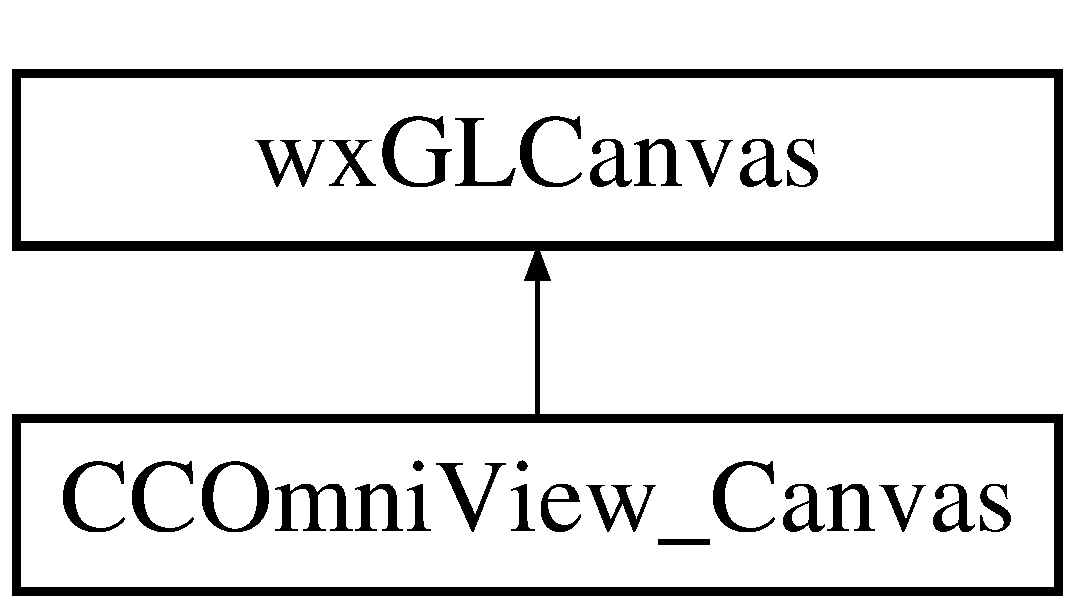
\includegraphics[height=2.000000cm]{a00049}
\end{center}
\end{figure}
\subsection*{Public Member Functions}
\begin{DoxyCompactItemize}
\item 
\hyperlink{a00049_a3fc09e3327a5620f2c3f7cb0fea28fab}{C\-C\-Omni\-View\-\_\-\-Canvas} (\hyperlink{a00015}{Animation\-View} $\ast$view, wx\-Window $\ast$frame, const wx\-Size \&size=wx\-Default\-Size)
\item 
\hyperlink{a00049_ae83d2497ad68db07582f904c8a80b8a6}{$\sim$\-C\-C\-Omni\-View\-\_\-\-Canvas} ()
\item 
void \hyperlink{a00049_a33a63201783809da9b89e35ce5573c15}{Set\-View} (\hyperlink{a00015}{Animation\-View} $\ast$view)
\item 
void \hyperlink{a00049_a8c35aa332886b0419dd6fd5dbe4c0835}{On\-Paint} (wx\-Paint\-Event \&event)
\item 
void \hyperlink{a00049_a208cb2d25466b7eaf97a546dba341653}{On\-Char} (wx\-Key\-Event \&event)
\item 
void \hyperlink{a00049_a18edf77ed13bce85a75ae9e401092671}{On\-Mouse\-Move} (wx\-Mouse\-Event \&event)
\item 
void \hyperlink{a00049_a5cbd3f39c70d8416e980ab05a46ce7f9}{On\-Cmd\-\_\-\-Follow\-Marcher} (int which)
\item 
void \hyperlink{a00049_a50aebf741afdc7732161ae12ac2a0eef}{On\-Cmd\-\_\-\-Save\-Camera\-Angle} (size\-\_\-t which)
\item 
void \hyperlink{a00049_aa84be7c65456cc042d78e666bec8cdb5}{On\-Cmd\-\_\-\-Go\-To\-Camera\-Angle} (size\-\_\-t which)
\item 
void \hyperlink{a00049_ac59d3c52c9759c500211373b9b540cb0}{On\-Cmd\-\_\-\-Toggle\-Crowd} ()
\item 
void \hyperlink{a00049_a94ca952ed179c60bd1789ee4029e9ec7}{On\-Cmd\-\_\-\-Toggle\-Marching} ()
\item 
void \hyperlink{a00049_ae520706e4e229f51be6d361cb8093830}{On\-Cmd\-\_\-\-Toggle\-Show\-Only\-Selected} ()
\end{DoxyCompactItemize}
\subsection*{Private Member Functions}
\begin{DoxyCompactItemize}
\item 
\hyperlink{a00110}{Marcher\-Info} \hyperlink{a00049_a44d29f5d38915f81d5231d78ac1a9eff}{Get\-Marcher\-Info} (size\-\_\-t which) const 
\item 
std\-::multimap$<$ double, \\*
\hyperlink{a00110}{Marcher\-Info} $>$ \hyperlink{a00049_aeda29351fb385ead8782a5dbdb3ddc79}{Parse\-And\-Draw3d\-Marchers} () const 
\item 
\hyperlink{a00049_a7a31d190a1e2ac6b51271ae7fde31d36}{wx\-D\-E\-C\-L\-A\-R\-E\-\_\-\-E\-V\-E\-N\-T\-\_\-\-T\-A\-B\-L\-E} ()
\end{DoxyCompactItemize}
\subsection*{Private Attributes}
\begin{DoxyCompactItemize}
\item 
boost\-::shared\-\_\-ptr\\*
$<$ \hyperlink{a00050}{C\-C\-Omni\-View\-\_\-\-G\-L\-Context} $>$ \hyperlink{a00049_a670422a2848a70cb52833a81061d990f}{m\-\_\-gl\-Context}
\item 
\hyperlink{a00015}{Animation\-View} $\ast$ \hyperlink{a00049_a6dc444adcccf109a636a4a8e5a3678c4}{m\-Animation\-View}
\item 
\hyperlink{a00154}{viewpoint\-\_\-t} \hyperlink{a00049_a68343cb2899d80c9cfc2053855232d3c}{m\-View\-Point}
\item 
int \hyperlink{a00049_a8ceffb3a7cd246765733c66cb1c794bb}{m\-Follow\-Marcher}
\item 
bool \hyperlink{a00049_af92114fc4626c7722ac50d5cdef22aad}{m\-Crowd\-On}
\item 
bool \hyperlink{a00049_a43acf3227cea9248543f2bcf955729f8}{m\-Show\-Only\-Selected}
\item 
bool \hyperlink{a00049_aed16d914b6dda9bb645e1e446fb70328}{m\-Show\-Marching}
\item 
float \hyperlink{a00049_a9aca6bb139d6088dc7a7d8b7769f653d}{m\-View\-Angle}
\item 
float \hyperlink{a00049_a187edb8b5697afd4ee616aab3400ea0e}{m\-View\-Angle\-Z}
\item 
float \hyperlink{a00049_a8c9ff38d651a4904b03f2a8a7995a3cd}{m\-F\-O\-V}
\item 
bool \hyperlink{a00049_a23011207227bebad7820a18caeaaa5fd}{m\-Shift\-Moving}
\item 
wx\-Point \hyperlink{a00049_a46bdf62d324feaf9c910ee8f5dee54e5}{m\-Start\-Shift\-Move\-Mouse\-Position}
\item 
float \hyperlink{a00049_a35c4764e86ce06efe20dab012ca2af53}{m\-Start\-Shift\-Move\-View\-Angle}
\item 
float \hyperlink{a00049_a5123da690cd5542692b58bbbfc189463}{m\-Start\-Shift\-Move\-View\-Angle\-Z}
\end{DoxyCompactItemize}


\subsection{Constructor \& Destructor Documentation}
\hypertarget{a00049_a3fc09e3327a5620f2c3f7cb0fea28fab}{\index{C\-C\-Omni\-View\-\_\-\-Canvas@{C\-C\-Omni\-View\-\_\-\-Canvas}!C\-C\-Omni\-View\-\_\-\-Canvas@{C\-C\-Omni\-View\-\_\-\-Canvas}}
\index{C\-C\-Omni\-View\-\_\-\-Canvas@{C\-C\-Omni\-View\-\_\-\-Canvas}!CCOmniView_Canvas@{C\-C\-Omni\-View\-\_\-\-Canvas}}
\subsubsection[{C\-C\-Omni\-View\-\_\-\-Canvas}]{\setlength{\rightskip}{0pt plus 5cm}C\-C\-Omni\-View\-\_\-\-Canvas\-::\-C\-C\-Omni\-View\-\_\-\-Canvas (
\begin{DoxyParamCaption}
\item[{{\bf Animation\-View} $\ast$}]{view, }
\item[{wx\-Window $\ast$}]{frame, }
\item[{const wx\-Size \&}]{size = {\ttfamily wxDefaultSize}}
\end{DoxyParamCaption}
)}}\label{a00049_a3fc09e3327a5620f2c3f7cb0fea28fab}
\hypertarget{a00049_ae83d2497ad68db07582f904c8a80b8a6}{\index{C\-C\-Omni\-View\-\_\-\-Canvas@{C\-C\-Omni\-View\-\_\-\-Canvas}!$\sim$\-C\-C\-Omni\-View\-\_\-\-Canvas@{$\sim$\-C\-C\-Omni\-View\-\_\-\-Canvas}}
\index{$\sim$\-C\-C\-Omni\-View\-\_\-\-Canvas@{$\sim$\-C\-C\-Omni\-View\-\_\-\-Canvas}!CCOmniView_Canvas@{C\-C\-Omni\-View\-\_\-\-Canvas}}
\subsubsection[{$\sim$\-C\-C\-Omni\-View\-\_\-\-Canvas}]{\setlength{\rightskip}{0pt plus 5cm}C\-C\-Omni\-View\-\_\-\-Canvas\-::$\sim$\-C\-C\-Omni\-View\-\_\-\-Canvas (
\begin{DoxyParamCaption}
{}
\end{DoxyParamCaption}
)}}\label{a00049_ae83d2497ad68db07582f904c8a80b8a6}


\subsection{Member Function Documentation}
\hypertarget{a00049_a44d29f5d38915f81d5231d78ac1a9eff}{\index{C\-C\-Omni\-View\-\_\-\-Canvas@{C\-C\-Omni\-View\-\_\-\-Canvas}!Get\-Marcher\-Info@{Get\-Marcher\-Info}}
\index{Get\-Marcher\-Info@{Get\-Marcher\-Info}!CCOmniView_Canvas@{C\-C\-Omni\-View\-\_\-\-Canvas}}
\subsubsection[{Get\-Marcher\-Info}]{\setlength{\rightskip}{0pt plus 5cm}{\bf Marcher\-Info} C\-C\-Omni\-View\-\_\-\-Canvas\-::\-Get\-Marcher\-Info (
\begin{DoxyParamCaption}
\item[{size\-\_\-t}]{which}
\end{DoxyParamCaption}
) const\hspace{0.3cm}{\ttfamily [private]}}}\label{a00049_a44d29f5d38915f81d5231d78ac1a9eff}
\hypertarget{a00049_a208cb2d25466b7eaf97a546dba341653}{\index{C\-C\-Omni\-View\-\_\-\-Canvas@{C\-C\-Omni\-View\-\_\-\-Canvas}!On\-Char@{On\-Char}}
\index{On\-Char@{On\-Char}!CCOmniView_Canvas@{C\-C\-Omni\-View\-\_\-\-Canvas}}
\subsubsection[{On\-Char}]{\setlength{\rightskip}{0pt plus 5cm}void C\-C\-Omni\-View\-\_\-\-Canvas\-::\-On\-Char (
\begin{DoxyParamCaption}
\item[{wx\-Key\-Event \&}]{event}
\end{DoxyParamCaption}
)}}\label{a00049_a208cb2d25466b7eaf97a546dba341653}
\hypertarget{a00049_a5cbd3f39c70d8416e980ab05a46ce7f9}{\index{C\-C\-Omni\-View\-\_\-\-Canvas@{C\-C\-Omni\-View\-\_\-\-Canvas}!On\-Cmd\-\_\-\-Follow\-Marcher@{On\-Cmd\-\_\-\-Follow\-Marcher}}
\index{On\-Cmd\-\_\-\-Follow\-Marcher@{On\-Cmd\-\_\-\-Follow\-Marcher}!CCOmniView_Canvas@{C\-C\-Omni\-View\-\_\-\-Canvas}}
\subsubsection[{On\-Cmd\-\_\-\-Follow\-Marcher}]{\setlength{\rightskip}{0pt plus 5cm}void C\-C\-Omni\-View\-\_\-\-Canvas\-::\-On\-Cmd\-\_\-\-Follow\-Marcher (
\begin{DoxyParamCaption}
\item[{int}]{which}
\end{DoxyParamCaption}
)}}\label{a00049_a5cbd3f39c70d8416e980ab05a46ce7f9}
\hypertarget{a00049_aa84be7c65456cc042d78e666bec8cdb5}{\index{C\-C\-Omni\-View\-\_\-\-Canvas@{C\-C\-Omni\-View\-\_\-\-Canvas}!On\-Cmd\-\_\-\-Go\-To\-Camera\-Angle@{On\-Cmd\-\_\-\-Go\-To\-Camera\-Angle}}
\index{On\-Cmd\-\_\-\-Go\-To\-Camera\-Angle@{On\-Cmd\-\_\-\-Go\-To\-Camera\-Angle}!CCOmniView_Canvas@{C\-C\-Omni\-View\-\_\-\-Canvas}}
\subsubsection[{On\-Cmd\-\_\-\-Go\-To\-Camera\-Angle}]{\setlength{\rightskip}{0pt plus 5cm}void C\-C\-Omni\-View\-\_\-\-Canvas\-::\-On\-Cmd\-\_\-\-Go\-To\-Camera\-Angle (
\begin{DoxyParamCaption}
\item[{size\-\_\-t}]{which}
\end{DoxyParamCaption}
)}}\label{a00049_aa84be7c65456cc042d78e666bec8cdb5}
\hypertarget{a00049_a50aebf741afdc7732161ae12ac2a0eef}{\index{C\-C\-Omni\-View\-\_\-\-Canvas@{C\-C\-Omni\-View\-\_\-\-Canvas}!On\-Cmd\-\_\-\-Save\-Camera\-Angle@{On\-Cmd\-\_\-\-Save\-Camera\-Angle}}
\index{On\-Cmd\-\_\-\-Save\-Camera\-Angle@{On\-Cmd\-\_\-\-Save\-Camera\-Angle}!CCOmniView_Canvas@{C\-C\-Omni\-View\-\_\-\-Canvas}}
\subsubsection[{On\-Cmd\-\_\-\-Save\-Camera\-Angle}]{\setlength{\rightskip}{0pt plus 5cm}void C\-C\-Omni\-View\-\_\-\-Canvas\-::\-On\-Cmd\-\_\-\-Save\-Camera\-Angle (
\begin{DoxyParamCaption}
\item[{size\-\_\-t}]{which}
\end{DoxyParamCaption}
)}}\label{a00049_a50aebf741afdc7732161ae12ac2a0eef}
\hypertarget{a00049_ac59d3c52c9759c500211373b9b540cb0}{\index{C\-C\-Omni\-View\-\_\-\-Canvas@{C\-C\-Omni\-View\-\_\-\-Canvas}!On\-Cmd\-\_\-\-Toggle\-Crowd@{On\-Cmd\-\_\-\-Toggle\-Crowd}}
\index{On\-Cmd\-\_\-\-Toggle\-Crowd@{On\-Cmd\-\_\-\-Toggle\-Crowd}!CCOmniView_Canvas@{C\-C\-Omni\-View\-\_\-\-Canvas}}
\subsubsection[{On\-Cmd\-\_\-\-Toggle\-Crowd}]{\setlength{\rightskip}{0pt plus 5cm}void C\-C\-Omni\-View\-\_\-\-Canvas\-::\-On\-Cmd\-\_\-\-Toggle\-Crowd (
\begin{DoxyParamCaption}
{}
\end{DoxyParamCaption}
)}}\label{a00049_ac59d3c52c9759c500211373b9b540cb0}
\hypertarget{a00049_a94ca952ed179c60bd1789ee4029e9ec7}{\index{C\-C\-Omni\-View\-\_\-\-Canvas@{C\-C\-Omni\-View\-\_\-\-Canvas}!On\-Cmd\-\_\-\-Toggle\-Marching@{On\-Cmd\-\_\-\-Toggle\-Marching}}
\index{On\-Cmd\-\_\-\-Toggle\-Marching@{On\-Cmd\-\_\-\-Toggle\-Marching}!CCOmniView_Canvas@{C\-C\-Omni\-View\-\_\-\-Canvas}}
\subsubsection[{On\-Cmd\-\_\-\-Toggle\-Marching}]{\setlength{\rightskip}{0pt plus 5cm}void C\-C\-Omni\-View\-\_\-\-Canvas\-::\-On\-Cmd\-\_\-\-Toggle\-Marching (
\begin{DoxyParamCaption}
{}
\end{DoxyParamCaption}
)}}\label{a00049_a94ca952ed179c60bd1789ee4029e9ec7}
\hypertarget{a00049_ae520706e4e229f51be6d361cb8093830}{\index{C\-C\-Omni\-View\-\_\-\-Canvas@{C\-C\-Omni\-View\-\_\-\-Canvas}!On\-Cmd\-\_\-\-Toggle\-Show\-Only\-Selected@{On\-Cmd\-\_\-\-Toggle\-Show\-Only\-Selected}}
\index{On\-Cmd\-\_\-\-Toggle\-Show\-Only\-Selected@{On\-Cmd\-\_\-\-Toggle\-Show\-Only\-Selected}!CCOmniView_Canvas@{C\-C\-Omni\-View\-\_\-\-Canvas}}
\subsubsection[{On\-Cmd\-\_\-\-Toggle\-Show\-Only\-Selected}]{\setlength{\rightskip}{0pt plus 5cm}void C\-C\-Omni\-View\-\_\-\-Canvas\-::\-On\-Cmd\-\_\-\-Toggle\-Show\-Only\-Selected (
\begin{DoxyParamCaption}
{}
\end{DoxyParamCaption}
)}}\label{a00049_ae520706e4e229f51be6d361cb8093830}
\hypertarget{a00049_a18edf77ed13bce85a75ae9e401092671}{\index{C\-C\-Omni\-View\-\_\-\-Canvas@{C\-C\-Omni\-View\-\_\-\-Canvas}!On\-Mouse\-Move@{On\-Mouse\-Move}}
\index{On\-Mouse\-Move@{On\-Mouse\-Move}!CCOmniView_Canvas@{C\-C\-Omni\-View\-\_\-\-Canvas}}
\subsubsection[{On\-Mouse\-Move}]{\setlength{\rightskip}{0pt plus 5cm}void C\-C\-Omni\-View\-\_\-\-Canvas\-::\-On\-Mouse\-Move (
\begin{DoxyParamCaption}
\item[{wx\-Mouse\-Event \&}]{event}
\end{DoxyParamCaption}
)}}\label{a00049_a18edf77ed13bce85a75ae9e401092671}
\hypertarget{a00049_a8c35aa332886b0419dd6fd5dbe4c0835}{\index{C\-C\-Omni\-View\-\_\-\-Canvas@{C\-C\-Omni\-View\-\_\-\-Canvas}!On\-Paint@{On\-Paint}}
\index{On\-Paint@{On\-Paint}!CCOmniView_Canvas@{C\-C\-Omni\-View\-\_\-\-Canvas}}
\subsubsection[{On\-Paint}]{\setlength{\rightskip}{0pt plus 5cm}void C\-C\-Omni\-View\-\_\-\-Canvas\-::\-On\-Paint (
\begin{DoxyParamCaption}
\item[{wx\-Paint\-Event \&}]{event}
\end{DoxyParamCaption}
)}}\label{a00049_a8c35aa332886b0419dd6fd5dbe4c0835}
\hypertarget{a00049_aeda29351fb385ead8782a5dbdb3ddc79}{\index{C\-C\-Omni\-View\-\_\-\-Canvas@{C\-C\-Omni\-View\-\_\-\-Canvas}!Parse\-And\-Draw3d\-Marchers@{Parse\-And\-Draw3d\-Marchers}}
\index{Parse\-And\-Draw3d\-Marchers@{Parse\-And\-Draw3d\-Marchers}!CCOmniView_Canvas@{C\-C\-Omni\-View\-\_\-\-Canvas}}
\subsubsection[{Parse\-And\-Draw3d\-Marchers}]{\setlength{\rightskip}{0pt plus 5cm}std\-::multimap$<$ double, {\bf Marcher\-Info} $>$ C\-C\-Omni\-View\-\_\-\-Canvas\-::\-Parse\-And\-Draw3d\-Marchers (
\begin{DoxyParamCaption}
{}
\end{DoxyParamCaption}
) const\hspace{0.3cm}{\ttfamily [private]}}}\label{a00049_aeda29351fb385ead8782a5dbdb3ddc79}
\hypertarget{a00049_a33a63201783809da9b89e35ce5573c15}{\index{C\-C\-Omni\-View\-\_\-\-Canvas@{C\-C\-Omni\-View\-\_\-\-Canvas}!Set\-View@{Set\-View}}
\index{Set\-View@{Set\-View}!CCOmniView_Canvas@{C\-C\-Omni\-View\-\_\-\-Canvas}}
\subsubsection[{Set\-View}]{\setlength{\rightskip}{0pt plus 5cm}void C\-C\-Omni\-View\-\_\-\-Canvas\-::\-Set\-View (
\begin{DoxyParamCaption}
\item[{{\bf Animation\-View} $\ast$}]{view}
\end{DoxyParamCaption}
)}}\label{a00049_a33a63201783809da9b89e35ce5573c15}
\hypertarget{a00049_a7a31d190a1e2ac6b51271ae7fde31d36}{\index{C\-C\-Omni\-View\-\_\-\-Canvas@{C\-C\-Omni\-View\-\_\-\-Canvas}!wx\-D\-E\-C\-L\-A\-R\-E\-\_\-\-E\-V\-E\-N\-T\-\_\-\-T\-A\-B\-L\-E@{wx\-D\-E\-C\-L\-A\-R\-E\-\_\-\-E\-V\-E\-N\-T\-\_\-\-T\-A\-B\-L\-E}}
\index{wx\-D\-E\-C\-L\-A\-R\-E\-\_\-\-E\-V\-E\-N\-T\-\_\-\-T\-A\-B\-L\-E@{wx\-D\-E\-C\-L\-A\-R\-E\-\_\-\-E\-V\-E\-N\-T\-\_\-\-T\-A\-B\-L\-E}!CCOmniView_Canvas@{C\-C\-Omni\-View\-\_\-\-Canvas}}
\subsubsection[{wx\-D\-E\-C\-L\-A\-R\-E\-\_\-\-E\-V\-E\-N\-T\-\_\-\-T\-A\-B\-L\-E}]{\setlength{\rightskip}{0pt plus 5cm}C\-C\-Omni\-View\-\_\-\-Canvas\-::wx\-D\-E\-C\-L\-A\-R\-E\-\_\-\-E\-V\-E\-N\-T\-\_\-\-T\-A\-B\-L\-E (
\begin{DoxyParamCaption}
{}
\end{DoxyParamCaption}
)\hspace{0.3cm}{\ttfamily [private]}}}\label{a00049_a7a31d190a1e2ac6b51271ae7fde31d36}


\subsection{Member Data Documentation}
\hypertarget{a00049_a670422a2848a70cb52833a81061d990f}{\index{C\-C\-Omni\-View\-\_\-\-Canvas@{C\-C\-Omni\-View\-\_\-\-Canvas}!m\-\_\-gl\-Context@{m\-\_\-gl\-Context}}
\index{m\-\_\-gl\-Context@{m\-\_\-gl\-Context}!CCOmniView_Canvas@{C\-C\-Omni\-View\-\_\-\-Canvas}}
\subsubsection[{m\-\_\-gl\-Context}]{\setlength{\rightskip}{0pt plus 5cm}boost\-::shared\-\_\-ptr$<${\bf C\-C\-Omni\-View\-\_\-\-G\-L\-Context}$>$ C\-C\-Omni\-View\-\_\-\-Canvas\-::m\-\_\-gl\-Context\hspace{0.3cm}{\ttfamily [private]}}}\label{a00049_a670422a2848a70cb52833a81061d990f}
\hypertarget{a00049_a6dc444adcccf109a636a4a8e5a3678c4}{\index{C\-C\-Omni\-View\-\_\-\-Canvas@{C\-C\-Omni\-View\-\_\-\-Canvas}!m\-Animation\-View@{m\-Animation\-View}}
\index{m\-Animation\-View@{m\-Animation\-View}!CCOmniView_Canvas@{C\-C\-Omni\-View\-\_\-\-Canvas}}
\subsubsection[{m\-Animation\-View}]{\setlength{\rightskip}{0pt plus 5cm}{\bf Animation\-View}$\ast$ C\-C\-Omni\-View\-\_\-\-Canvas\-::m\-Animation\-View\hspace{0.3cm}{\ttfamily [private]}}}\label{a00049_a6dc444adcccf109a636a4a8e5a3678c4}
\hypertarget{a00049_af92114fc4626c7722ac50d5cdef22aad}{\index{C\-C\-Omni\-View\-\_\-\-Canvas@{C\-C\-Omni\-View\-\_\-\-Canvas}!m\-Crowd\-On@{m\-Crowd\-On}}
\index{m\-Crowd\-On@{m\-Crowd\-On}!CCOmniView_Canvas@{C\-C\-Omni\-View\-\_\-\-Canvas}}
\subsubsection[{m\-Crowd\-On}]{\setlength{\rightskip}{0pt plus 5cm}bool C\-C\-Omni\-View\-\_\-\-Canvas\-::m\-Crowd\-On\hspace{0.3cm}{\ttfamily [private]}}}\label{a00049_af92114fc4626c7722ac50d5cdef22aad}
\hypertarget{a00049_a8ceffb3a7cd246765733c66cb1c794bb}{\index{C\-C\-Omni\-View\-\_\-\-Canvas@{C\-C\-Omni\-View\-\_\-\-Canvas}!m\-Follow\-Marcher@{m\-Follow\-Marcher}}
\index{m\-Follow\-Marcher@{m\-Follow\-Marcher}!CCOmniView_Canvas@{C\-C\-Omni\-View\-\_\-\-Canvas}}
\subsubsection[{m\-Follow\-Marcher}]{\setlength{\rightskip}{0pt plus 5cm}int C\-C\-Omni\-View\-\_\-\-Canvas\-::m\-Follow\-Marcher\hspace{0.3cm}{\ttfamily [private]}}}\label{a00049_a8ceffb3a7cd246765733c66cb1c794bb}
\hypertarget{a00049_a8c9ff38d651a4904b03f2a8a7995a3cd}{\index{C\-C\-Omni\-View\-\_\-\-Canvas@{C\-C\-Omni\-View\-\_\-\-Canvas}!m\-F\-O\-V@{m\-F\-O\-V}}
\index{m\-F\-O\-V@{m\-F\-O\-V}!CCOmniView_Canvas@{C\-C\-Omni\-View\-\_\-\-Canvas}}
\subsubsection[{m\-F\-O\-V}]{\setlength{\rightskip}{0pt plus 5cm}float C\-C\-Omni\-View\-\_\-\-Canvas\-::m\-F\-O\-V\hspace{0.3cm}{\ttfamily [private]}}}\label{a00049_a8c9ff38d651a4904b03f2a8a7995a3cd}
\hypertarget{a00049_a23011207227bebad7820a18caeaaa5fd}{\index{C\-C\-Omni\-View\-\_\-\-Canvas@{C\-C\-Omni\-View\-\_\-\-Canvas}!m\-Shift\-Moving@{m\-Shift\-Moving}}
\index{m\-Shift\-Moving@{m\-Shift\-Moving}!CCOmniView_Canvas@{C\-C\-Omni\-View\-\_\-\-Canvas}}
\subsubsection[{m\-Shift\-Moving}]{\setlength{\rightskip}{0pt plus 5cm}bool C\-C\-Omni\-View\-\_\-\-Canvas\-::m\-Shift\-Moving\hspace{0.3cm}{\ttfamily [private]}}}\label{a00049_a23011207227bebad7820a18caeaaa5fd}
\hypertarget{a00049_aed16d914b6dda9bb645e1e446fb70328}{\index{C\-C\-Omni\-View\-\_\-\-Canvas@{C\-C\-Omni\-View\-\_\-\-Canvas}!m\-Show\-Marching@{m\-Show\-Marching}}
\index{m\-Show\-Marching@{m\-Show\-Marching}!CCOmniView_Canvas@{C\-C\-Omni\-View\-\_\-\-Canvas}}
\subsubsection[{m\-Show\-Marching}]{\setlength{\rightskip}{0pt plus 5cm}bool C\-C\-Omni\-View\-\_\-\-Canvas\-::m\-Show\-Marching\hspace{0.3cm}{\ttfamily [private]}}}\label{a00049_aed16d914b6dda9bb645e1e446fb70328}
\hypertarget{a00049_a43acf3227cea9248543f2bcf955729f8}{\index{C\-C\-Omni\-View\-\_\-\-Canvas@{C\-C\-Omni\-View\-\_\-\-Canvas}!m\-Show\-Only\-Selected@{m\-Show\-Only\-Selected}}
\index{m\-Show\-Only\-Selected@{m\-Show\-Only\-Selected}!CCOmniView_Canvas@{C\-C\-Omni\-View\-\_\-\-Canvas}}
\subsubsection[{m\-Show\-Only\-Selected}]{\setlength{\rightskip}{0pt plus 5cm}bool C\-C\-Omni\-View\-\_\-\-Canvas\-::m\-Show\-Only\-Selected\hspace{0.3cm}{\ttfamily [private]}}}\label{a00049_a43acf3227cea9248543f2bcf955729f8}
\hypertarget{a00049_a46bdf62d324feaf9c910ee8f5dee54e5}{\index{C\-C\-Omni\-View\-\_\-\-Canvas@{C\-C\-Omni\-View\-\_\-\-Canvas}!m\-Start\-Shift\-Move\-Mouse\-Position@{m\-Start\-Shift\-Move\-Mouse\-Position}}
\index{m\-Start\-Shift\-Move\-Mouse\-Position@{m\-Start\-Shift\-Move\-Mouse\-Position}!CCOmniView_Canvas@{C\-C\-Omni\-View\-\_\-\-Canvas}}
\subsubsection[{m\-Start\-Shift\-Move\-Mouse\-Position}]{\setlength{\rightskip}{0pt plus 5cm}wx\-Point C\-C\-Omni\-View\-\_\-\-Canvas\-::m\-Start\-Shift\-Move\-Mouse\-Position\hspace{0.3cm}{\ttfamily [private]}}}\label{a00049_a46bdf62d324feaf9c910ee8f5dee54e5}
\hypertarget{a00049_a35c4764e86ce06efe20dab012ca2af53}{\index{C\-C\-Omni\-View\-\_\-\-Canvas@{C\-C\-Omni\-View\-\_\-\-Canvas}!m\-Start\-Shift\-Move\-View\-Angle@{m\-Start\-Shift\-Move\-View\-Angle}}
\index{m\-Start\-Shift\-Move\-View\-Angle@{m\-Start\-Shift\-Move\-View\-Angle}!CCOmniView_Canvas@{C\-C\-Omni\-View\-\_\-\-Canvas}}
\subsubsection[{m\-Start\-Shift\-Move\-View\-Angle}]{\setlength{\rightskip}{0pt plus 5cm}float C\-C\-Omni\-View\-\_\-\-Canvas\-::m\-Start\-Shift\-Move\-View\-Angle\hspace{0.3cm}{\ttfamily [private]}}}\label{a00049_a35c4764e86ce06efe20dab012ca2af53}
\hypertarget{a00049_a5123da690cd5542692b58bbbfc189463}{\index{C\-C\-Omni\-View\-\_\-\-Canvas@{C\-C\-Omni\-View\-\_\-\-Canvas}!m\-Start\-Shift\-Move\-View\-Angle\-Z@{m\-Start\-Shift\-Move\-View\-Angle\-Z}}
\index{m\-Start\-Shift\-Move\-View\-Angle\-Z@{m\-Start\-Shift\-Move\-View\-Angle\-Z}!CCOmniView_Canvas@{C\-C\-Omni\-View\-\_\-\-Canvas}}
\subsubsection[{m\-Start\-Shift\-Move\-View\-Angle\-Z}]{\setlength{\rightskip}{0pt plus 5cm}float C\-C\-Omni\-View\-\_\-\-Canvas\-::m\-Start\-Shift\-Move\-View\-Angle\-Z\hspace{0.3cm}{\ttfamily [private]}}}\label{a00049_a5123da690cd5542692b58bbbfc189463}
\hypertarget{a00049_a9aca6bb139d6088dc7a7d8b7769f653d}{\index{C\-C\-Omni\-View\-\_\-\-Canvas@{C\-C\-Omni\-View\-\_\-\-Canvas}!m\-View\-Angle@{m\-View\-Angle}}
\index{m\-View\-Angle@{m\-View\-Angle}!CCOmniView_Canvas@{C\-C\-Omni\-View\-\_\-\-Canvas}}
\subsubsection[{m\-View\-Angle}]{\setlength{\rightskip}{0pt plus 5cm}float C\-C\-Omni\-View\-\_\-\-Canvas\-::m\-View\-Angle\hspace{0.3cm}{\ttfamily [private]}}}\label{a00049_a9aca6bb139d6088dc7a7d8b7769f653d}
\hypertarget{a00049_a187edb8b5697afd4ee616aab3400ea0e}{\index{C\-C\-Omni\-View\-\_\-\-Canvas@{C\-C\-Omni\-View\-\_\-\-Canvas}!m\-View\-Angle\-Z@{m\-View\-Angle\-Z}}
\index{m\-View\-Angle\-Z@{m\-View\-Angle\-Z}!CCOmniView_Canvas@{C\-C\-Omni\-View\-\_\-\-Canvas}}
\subsubsection[{m\-View\-Angle\-Z}]{\setlength{\rightskip}{0pt plus 5cm}float C\-C\-Omni\-View\-\_\-\-Canvas\-::m\-View\-Angle\-Z\hspace{0.3cm}{\ttfamily [private]}}}\label{a00049_a187edb8b5697afd4ee616aab3400ea0e}
\hypertarget{a00049_a68343cb2899d80c9cfc2053855232d3c}{\index{C\-C\-Omni\-View\-\_\-\-Canvas@{C\-C\-Omni\-View\-\_\-\-Canvas}!m\-View\-Point@{m\-View\-Point}}
\index{m\-View\-Point@{m\-View\-Point}!CCOmniView_Canvas@{C\-C\-Omni\-View\-\_\-\-Canvas}}
\subsubsection[{m\-View\-Point}]{\setlength{\rightskip}{0pt plus 5cm}{\bf viewpoint\-\_\-t} C\-C\-Omni\-View\-\_\-\-Canvas\-::m\-View\-Point\hspace{0.3cm}{\ttfamily [private]}}}\label{a00049_a68343cb2899d80c9cfc2053855232d3c}


The documentation for this class was generated from the following files\-:\begin{DoxyCompactItemize}
\item 
src/\hyperlink{a00185}{cc\-\_\-omniview\-\_\-canvas.\-h}\item 
src/\hyperlink{a00184}{cc\-\_\-omniview\-\_\-canvas.\-cpp}\end{DoxyCompactItemize}

\hypertarget{a00050}{\section{C\-C\-Omni\-View\-\_\-\-G\-L\-Context Class Reference}
\label{a00050}\index{C\-C\-Omni\-View\-\_\-\-G\-L\-Context@{C\-C\-Omni\-View\-\_\-\-G\-L\-Context}}
}
Inheritance diagram for C\-C\-Omni\-View\-\_\-\-G\-L\-Context\-:\begin{figure}[H]
\begin{center}
\leavevmode
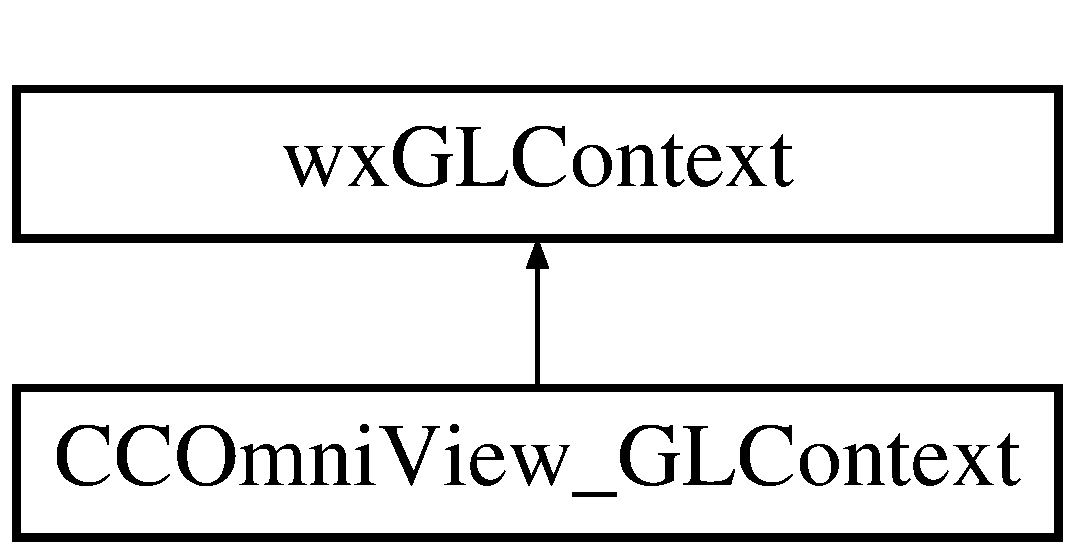
\includegraphics[height=2.000000cm]{a00050}
\end{center}
\end{figure}
\subsection*{Public Member Functions}
\begin{DoxyCompactItemize}
\item 
\hyperlink{a00050_ac66f48acb1583ae25a6ed770c746ba6a}{C\-C\-Omni\-View\-\_\-\-G\-L\-Context} (wx\-G\-L\-Canvas $\ast$canvas)
\item 
void \hyperlink{a00050_aca426c616d0fb783feafe7de5870e124}{Draw\-Field} (float Field\-E\-W, float Field\-N\-S, bool crowd\-On)
\item 
void \hyperlink{a00050_aae01a0d26f053eccd0688f6842708f49}{Draw3d\-Marcher} (const \hyperlink{a00110}{Marcher\-Info} \&info, const \hyperlink{a00154}{viewpoint\-\_\-t} \&viewpoint, \hyperlink{a00184_aaa2f3b8c2e888a44317f26cff6f9bf7d}{Which\-Marching\-Style} style)
\item 
bool \hyperlink{a00050_af821fc86e6add66e885b5d8150017d03}{Use\-For\-Lines} (const wx\-Image \&lines)
\end{DoxyCompactItemize}
\subsection*{Private Attributes}
\begin{DoxyCompactItemize}
\item 
G\-Luint \hyperlink{a00050_a00cadfd974ac7c904eba18fded443089}{m\-\_\-textures} \mbox{[}\hyperlink{a00184_a7eb3720b4254c41f480c577182480c7baddebdce3e8697071b6d1b87d0a0794fb}{k\-Image\-Last}\mbox{]}
\end{DoxyCompactItemize}


\subsection{Constructor \& Destructor Documentation}
\hypertarget{a00050_ac66f48acb1583ae25a6ed770c746ba6a}{\index{C\-C\-Omni\-View\-\_\-\-G\-L\-Context@{C\-C\-Omni\-View\-\_\-\-G\-L\-Context}!C\-C\-Omni\-View\-\_\-\-G\-L\-Context@{C\-C\-Omni\-View\-\_\-\-G\-L\-Context}}
\index{C\-C\-Omni\-View\-\_\-\-G\-L\-Context@{C\-C\-Omni\-View\-\_\-\-G\-L\-Context}!CCOmniView_GLContext@{C\-C\-Omni\-View\-\_\-\-G\-L\-Context}}
\subsubsection[{C\-C\-Omni\-View\-\_\-\-G\-L\-Context}]{\setlength{\rightskip}{0pt plus 5cm}C\-C\-Omni\-View\-\_\-\-G\-L\-Context\-::\-C\-C\-Omni\-View\-\_\-\-G\-L\-Context (
\begin{DoxyParamCaption}
\item[{wx\-G\-L\-Canvas $\ast$}]{canvas}
\end{DoxyParamCaption}
)}}\label{a00050_ac66f48acb1583ae25a6ed770c746ba6a}


\subsection{Member Function Documentation}
\hypertarget{a00050_aae01a0d26f053eccd0688f6842708f49}{\index{C\-C\-Omni\-View\-\_\-\-G\-L\-Context@{C\-C\-Omni\-View\-\_\-\-G\-L\-Context}!Draw3d\-Marcher@{Draw3d\-Marcher}}
\index{Draw3d\-Marcher@{Draw3d\-Marcher}!CCOmniView_GLContext@{C\-C\-Omni\-View\-\_\-\-G\-L\-Context}}
\subsubsection[{Draw3d\-Marcher}]{\setlength{\rightskip}{0pt plus 5cm}void C\-C\-Omni\-View\-\_\-\-G\-L\-Context\-::\-Draw3d\-Marcher (
\begin{DoxyParamCaption}
\item[{const {\bf Marcher\-Info} \&}]{info, }
\item[{const {\bf viewpoint\-\_\-t} \&}]{viewpoint, }
\item[{{\bf Which\-Marching\-Style}}]{style}
\end{DoxyParamCaption}
)}}\label{a00050_aae01a0d26f053eccd0688f6842708f49}
\hypertarget{a00050_aca426c616d0fb783feafe7de5870e124}{\index{C\-C\-Omni\-View\-\_\-\-G\-L\-Context@{C\-C\-Omni\-View\-\_\-\-G\-L\-Context}!Draw\-Field@{Draw\-Field}}
\index{Draw\-Field@{Draw\-Field}!CCOmniView_GLContext@{C\-C\-Omni\-View\-\_\-\-G\-L\-Context}}
\subsubsection[{Draw\-Field}]{\setlength{\rightskip}{0pt plus 5cm}void C\-C\-Omni\-View\-\_\-\-G\-L\-Context\-::\-Draw\-Field (
\begin{DoxyParamCaption}
\item[{float}]{Field\-E\-W, }
\item[{float}]{Field\-N\-S, }
\item[{bool}]{crowd\-On}
\end{DoxyParamCaption}
)}}\label{a00050_aca426c616d0fb783feafe7de5870e124}
\hypertarget{a00050_af821fc86e6add66e885b5d8150017d03}{\index{C\-C\-Omni\-View\-\_\-\-G\-L\-Context@{C\-C\-Omni\-View\-\_\-\-G\-L\-Context}!Use\-For\-Lines@{Use\-For\-Lines}}
\index{Use\-For\-Lines@{Use\-For\-Lines}!CCOmniView_GLContext@{C\-C\-Omni\-View\-\_\-\-G\-L\-Context}}
\subsubsection[{Use\-For\-Lines}]{\setlength{\rightskip}{0pt plus 5cm}bool C\-C\-Omni\-View\-\_\-\-G\-L\-Context\-::\-Use\-For\-Lines (
\begin{DoxyParamCaption}
\item[{const wx\-Image \&}]{lines}
\end{DoxyParamCaption}
)}}\label{a00050_af821fc86e6add66e885b5d8150017d03}


\subsection{Member Data Documentation}
\hypertarget{a00050_a00cadfd974ac7c904eba18fded443089}{\index{C\-C\-Omni\-View\-\_\-\-G\-L\-Context@{C\-C\-Omni\-View\-\_\-\-G\-L\-Context}!m\-\_\-textures@{m\-\_\-textures}}
\index{m\-\_\-textures@{m\-\_\-textures}!CCOmniView_GLContext@{C\-C\-Omni\-View\-\_\-\-G\-L\-Context}}
\subsubsection[{m\-\_\-textures}]{\setlength{\rightskip}{0pt plus 5cm}G\-Luint C\-C\-Omni\-View\-\_\-\-G\-L\-Context\-::m\-\_\-textures\mbox{[}{\bf k\-Image\-Last}\mbox{]}\hspace{0.3cm}{\ttfamily [private]}}}\label{a00050_a00cadfd974ac7c904eba18fded443089}


The documentation for this class was generated from the following file\-:\begin{DoxyCompactItemize}
\item 
src/\hyperlink{a00184}{cc\-\_\-omniview\-\_\-canvas.\-cpp}\end{DoxyCompactItemize}

\hypertarget{a00051}{\section{Choose\-Show\-Mode\-Wizard Class Reference}
\label{a00051}\index{Choose\-Show\-Mode\-Wizard@{Choose\-Show\-Mode\-Wizard}}
}


{\ttfamily \#include $<$setup\-\_\-wizards.\-h$>$}

Inheritance diagram for Choose\-Show\-Mode\-Wizard\-:\begin{figure}[H]
\begin{center}
\leavevmode
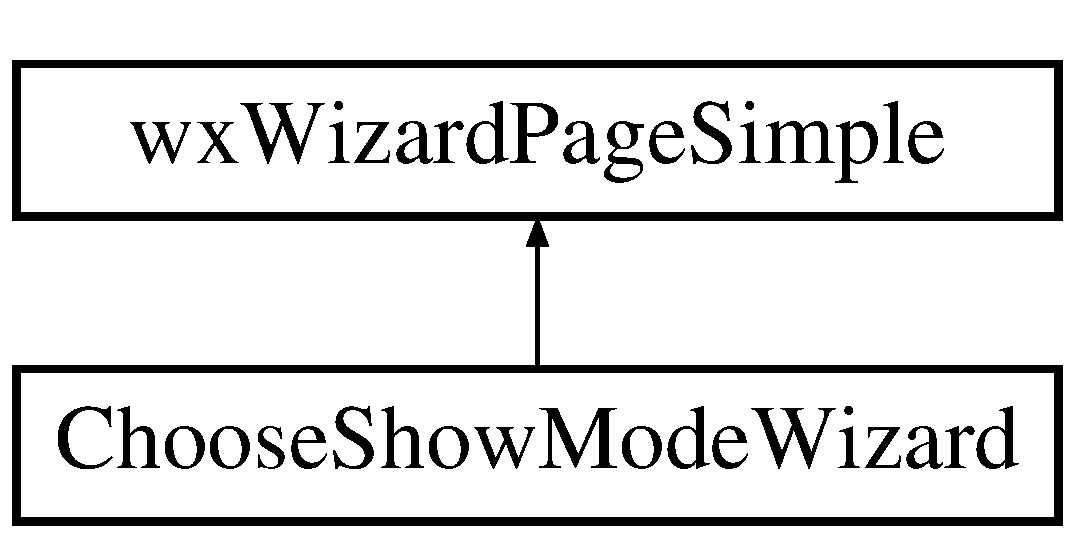
\includegraphics[height=2.000000cm]{a00051}
\end{center}
\end{figure}
\subsection*{Public Member Functions}
\begin{DoxyCompactItemize}
\item 
\hyperlink{a00051_a3da099bce84dfcf67b712dc723d14bf6}{Choose\-Show\-Mode\-Wizard} (wx\-Wizard $\ast$parent)
\item 
wx\-String \hyperlink{a00051_abb0a6b9caee7ffbce23fa635f5877eb8}{Get\-Value} ()
\end{DoxyCompactItemize}
\subsection*{Private Attributes}
\begin{DoxyCompactItemize}
\item 
wx\-Array\-String \hyperlink{a00051_a8500e29b611471ee74ab0e0530487d6f}{mode\-Strings}
\item 
wx\-Choice $\ast$ \hyperlink{a00051_ab348bdfb5863214f3bab95c4a636af62}{m\-Choice}
\end{DoxyCompactItemize}


\subsection{Constructor \& Destructor Documentation}
\hypertarget{a00051_a3da099bce84dfcf67b712dc723d14bf6}{\index{Choose\-Show\-Mode\-Wizard@{Choose\-Show\-Mode\-Wizard}!Choose\-Show\-Mode\-Wizard@{Choose\-Show\-Mode\-Wizard}}
\index{Choose\-Show\-Mode\-Wizard@{Choose\-Show\-Mode\-Wizard}!ChooseShowModeWizard@{Choose\-Show\-Mode\-Wizard}}
\subsubsection[{Choose\-Show\-Mode\-Wizard}]{\setlength{\rightskip}{0pt plus 5cm}Choose\-Show\-Mode\-Wizard\-::\-Choose\-Show\-Mode\-Wizard (
\begin{DoxyParamCaption}
\item[{wx\-Wizard $\ast$}]{parent}
\end{DoxyParamCaption}
)}}\label{a00051_a3da099bce84dfcf67b712dc723d14bf6}


\subsection{Member Function Documentation}
\hypertarget{a00051_abb0a6b9caee7ffbce23fa635f5877eb8}{\index{Choose\-Show\-Mode\-Wizard@{Choose\-Show\-Mode\-Wizard}!Get\-Value@{Get\-Value}}
\index{Get\-Value@{Get\-Value}!ChooseShowModeWizard@{Choose\-Show\-Mode\-Wizard}}
\subsubsection[{Get\-Value}]{\setlength{\rightskip}{0pt plus 5cm}wx\-String Choose\-Show\-Mode\-Wizard\-::\-Get\-Value (
\begin{DoxyParamCaption}
{}
\end{DoxyParamCaption}
)}}\label{a00051_abb0a6b9caee7ffbce23fa635f5877eb8}


\subsection{Member Data Documentation}
\hypertarget{a00051_ab348bdfb5863214f3bab95c4a636af62}{\index{Choose\-Show\-Mode\-Wizard@{Choose\-Show\-Mode\-Wizard}!m\-Choice@{m\-Choice}}
\index{m\-Choice@{m\-Choice}!ChooseShowModeWizard@{Choose\-Show\-Mode\-Wizard}}
\subsubsection[{m\-Choice}]{\setlength{\rightskip}{0pt plus 5cm}wx\-Choice$\ast$ Choose\-Show\-Mode\-Wizard\-::m\-Choice\hspace{0.3cm}{\ttfamily [private]}}}\label{a00051_ab348bdfb5863214f3bab95c4a636af62}
\hypertarget{a00051_a8500e29b611471ee74ab0e0530487d6f}{\index{Choose\-Show\-Mode\-Wizard@{Choose\-Show\-Mode\-Wizard}!mode\-Strings@{mode\-Strings}}
\index{mode\-Strings@{mode\-Strings}!ChooseShowModeWizard@{Choose\-Show\-Mode\-Wizard}}
\subsubsection[{mode\-Strings}]{\setlength{\rightskip}{0pt plus 5cm}wx\-Array\-String Choose\-Show\-Mode\-Wizard\-::mode\-Strings\hspace{0.3cm}{\ttfamily [private]}}}\label{a00051_a8500e29b611471ee74ab0e0530487d6f}


The documentation for this class was generated from the following files\-:\begin{DoxyCompactItemize}
\item 
src/\hyperlink{a00243}{setup\-\_\-wizards.\-h}\item 
src/\hyperlink{a00242}{setup\-\_\-wizards.\-cpp}\end{DoxyCompactItemize}

\hypertarget{a00052}{\section{Cont\-Func\-Dir Class Reference}
\label{a00052}\index{Cont\-Func\-Dir@{Cont\-Func\-Dir}}
}


{\ttfamily \#include $<$cont.\-h$>$}

Inheritance diagram for Cont\-Func\-Dir\-:\begin{figure}[H]
\begin{center}
\leavevmode
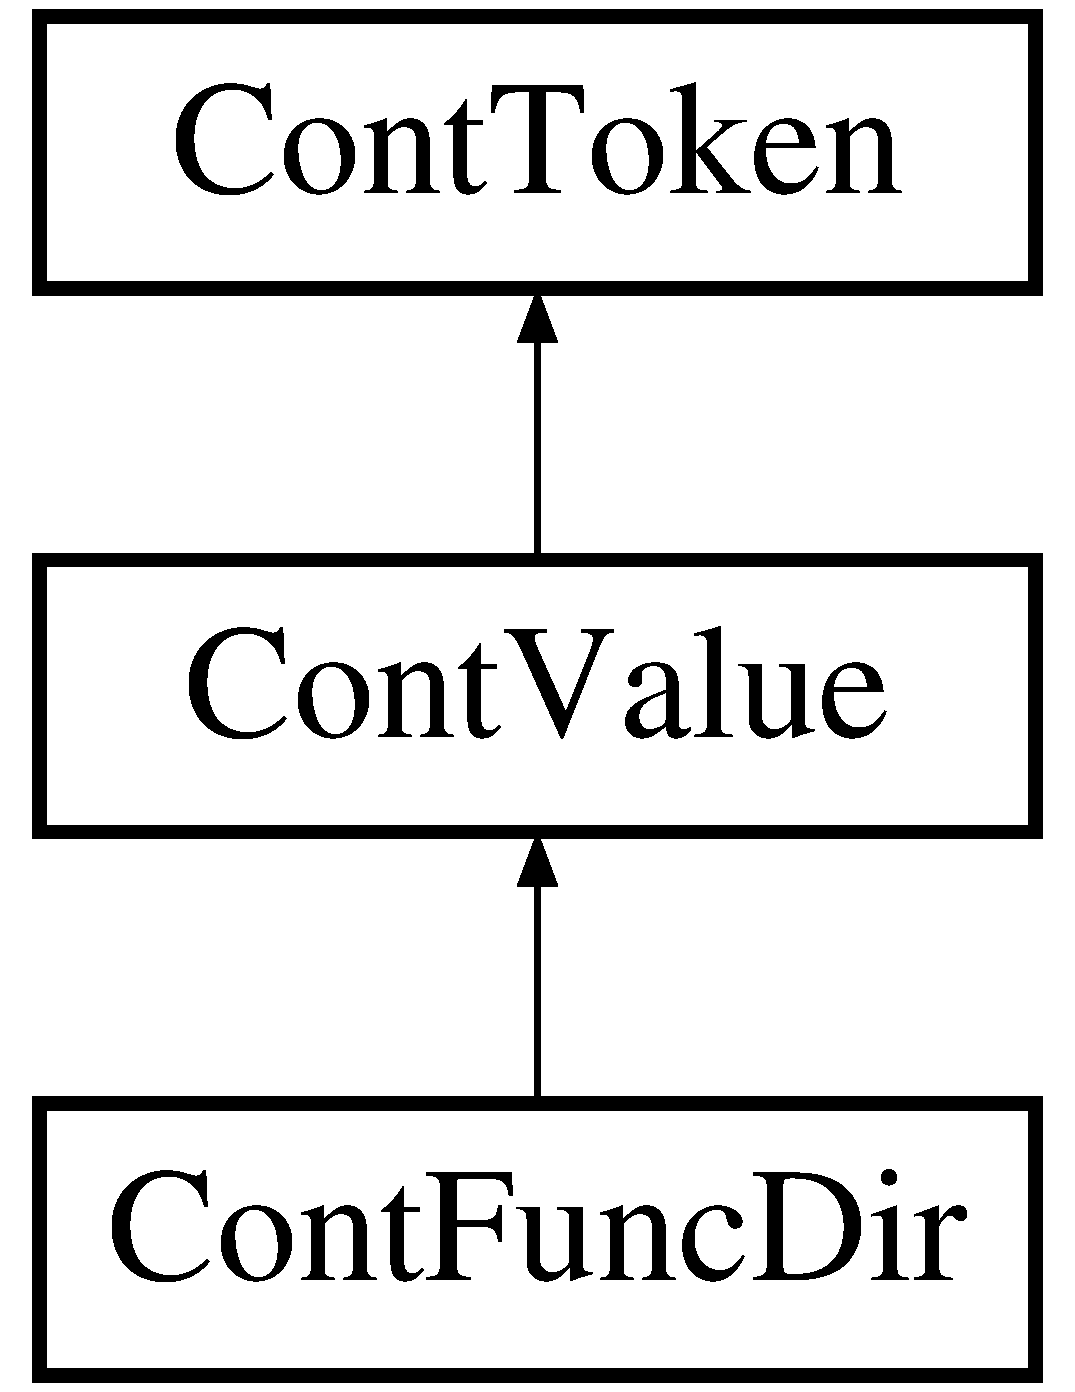
\includegraphics[height=3.000000cm]{a00052}
\end{center}
\end{figure}
\subsection*{Public Member Functions}
\begin{DoxyCompactItemize}
\item 
\hyperlink{a00052_a0ece4d71b207011e42e531c5721a1fba}{Cont\-Func\-Dir} (\hyperlink{a00062}{Cont\-Point} $\ast$p)
\item 
virtual \hyperlink{a00052_af3c5d0aa1a9a3fe183bfff5c412f4694}{$\sim$\-Cont\-Func\-Dir} ()
\item 
virtual float \hyperlink{a00052_ac2fbca045989da578c7fe551c0eadeea}{Get} (\hyperlink{a00007}{Animate\-Compile} $\ast$anim) const 
\end{DoxyCompactItemize}
\subsection*{Private Attributes}
\begin{DoxyCompactItemize}
\item 
\hyperlink{a00062}{Cont\-Point} $\ast$ \hyperlink{a00052_aae431b4159623c57365bf905bbe8de00}{pnt}
\end{DoxyCompactItemize}
\subsection*{Additional Inherited Members}


\subsection{Constructor \& Destructor Documentation}
\hypertarget{a00052_a0ece4d71b207011e42e531c5721a1fba}{\index{Cont\-Func\-Dir@{Cont\-Func\-Dir}!Cont\-Func\-Dir@{Cont\-Func\-Dir}}
\index{Cont\-Func\-Dir@{Cont\-Func\-Dir}!ContFuncDir@{Cont\-Func\-Dir}}
\subsubsection[{Cont\-Func\-Dir}]{\setlength{\rightskip}{0pt plus 5cm}Cont\-Func\-Dir\-::\-Cont\-Func\-Dir (
\begin{DoxyParamCaption}
\item[{{\bf Cont\-Point} $\ast$}]{p}
\end{DoxyParamCaption}
)\hspace{0.3cm}{\ttfamily [inline]}}}\label{a00052_a0ece4d71b207011e42e531c5721a1fba}
\hypertarget{a00052_af3c5d0aa1a9a3fe183bfff5c412f4694}{\index{Cont\-Func\-Dir@{Cont\-Func\-Dir}!$\sim$\-Cont\-Func\-Dir@{$\sim$\-Cont\-Func\-Dir}}
\index{$\sim$\-Cont\-Func\-Dir@{$\sim$\-Cont\-Func\-Dir}!ContFuncDir@{Cont\-Func\-Dir}}
\subsubsection[{$\sim$\-Cont\-Func\-Dir}]{\setlength{\rightskip}{0pt plus 5cm}Cont\-Func\-Dir\-::$\sim$\-Cont\-Func\-Dir (
\begin{DoxyParamCaption}
{}
\end{DoxyParamCaption}
)\hspace{0.3cm}{\ttfamily [virtual]}}}\label{a00052_af3c5d0aa1a9a3fe183bfff5c412f4694}


\subsection{Member Function Documentation}
\hypertarget{a00052_ac2fbca045989da578c7fe551c0eadeea}{\index{Cont\-Func\-Dir@{Cont\-Func\-Dir}!Get@{Get}}
\index{Get@{Get}!ContFuncDir@{Cont\-Func\-Dir}}
\subsubsection[{Get}]{\setlength{\rightskip}{0pt plus 5cm}float Cont\-Func\-Dir\-::\-Get (
\begin{DoxyParamCaption}
\item[{{\bf Animate\-Compile} $\ast$}]{anim}
\end{DoxyParamCaption}
) const\hspace{0.3cm}{\ttfamily [virtual]}}}\label{a00052_ac2fbca045989da578c7fe551c0eadeea}


Implements \hyperlink{a00086_ae3ce98084899bf1a873a1ec6bf15116e}{Cont\-Value}.



\subsection{Member Data Documentation}
\hypertarget{a00052_aae431b4159623c57365bf905bbe8de00}{\index{Cont\-Func\-Dir@{Cont\-Func\-Dir}!pnt@{pnt}}
\index{pnt@{pnt}!ContFuncDir@{Cont\-Func\-Dir}}
\subsubsection[{pnt}]{\setlength{\rightskip}{0pt plus 5cm}{\bf Cont\-Point}$\ast$ Cont\-Func\-Dir\-::pnt\hspace{0.3cm}{\ttfamily [private]}}}\label{a00052_aae431b4159623c57365bf905bbe8de00}


The documentation for this class was generated from the following files\-:\begin{DoxyCompactItemize}
\item 
src/core/\hyperlink{a00218}{cont.\-h}\item 
src/core/\hyperlink{a00217}{cont.\-cpp}\end{DoxyCompactItemize}

\hypertarget{a00053}{\section{Cont\-Func\-Dir\-From Class Reference}
\label{a00053}\index{Cont\-Func\-Dir\-From@{Cont\-Func\-Dir\-From}}
}


{\ttfamily \#include $<$cont.\-h$>$}

Inheritance diagram for Cont\-Func\-Dir\-From\-:\begin{figure}[H]
\begin{center}
\leavevmode
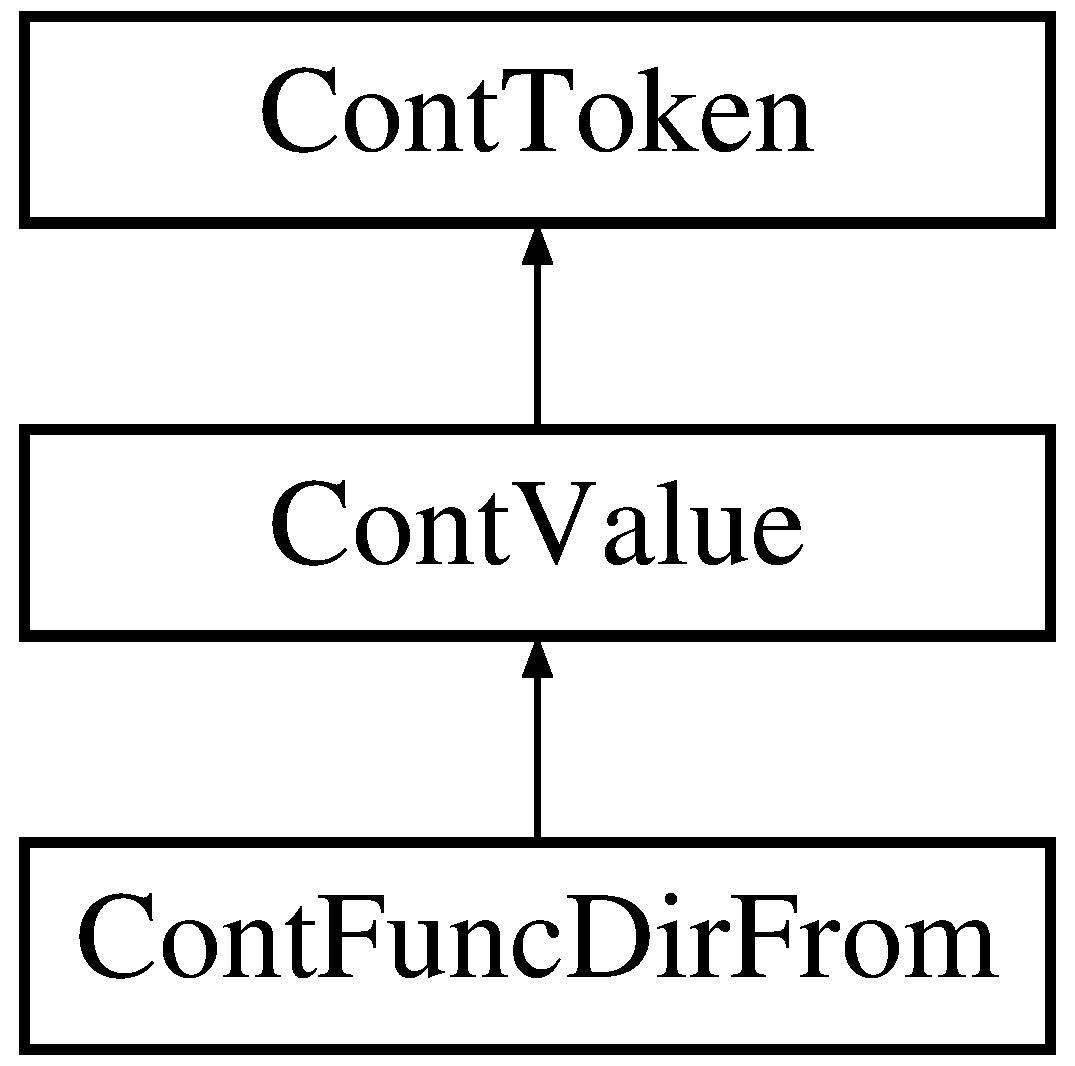
\includegraphics[height=3.000000cm]{a00053}
\end{center}
\end{figure}
\subsection*{Public Member Functions}
\begin{DoxyCompactItemize}
\item 
\hyperlink{a00053_aad1f01170a3aa55f68c85d0564325005}{Cont\-Func\-Dir\-From} (\hyperlink{a00062}{Cont\-Point} $\ast$start, \hyperlink{a00062}{Cont\-Point} $\ast$end)
\item 
virtual \hyperlink{a00053_a773fd565cfb24280beacf0a916eddf2b}{$\sim$\-Cont\-Func\-Dir\-From} ()
\item 
virtual float \hyperlink{a00053_a7bf25238dce61c2810ef200764a86c8a}{Get} (\hyperlink{a00007}{Animate\-Compile} $\ast$anim) const 
\end{DoxyCompactItemize}
\subsection*{Private Attributes}
\begin{DoxyCompactItemize}
\item 
\hyperlink{a00062}{Cont\-Point} $\ast$ \hyperlink{a00053_a057385fa5f34bec3e9691e3a7a9a6b9a}{pnt\-\_\-start}
\item 
\hyperlink{a00062}{Cont\-Point} $\ast$ \hyperlink{a00053_a3d16a2d6d1a2b702c628fc988ac1d541}{pnt\-\_\-end}
\end{DoxyCompactItemize}
\subsection*{Additional Inherited Members}


\subsection{Constructor \& Destructor Documentation}
\hypertarget{a00053_aad1f01170a3aa55f68c85d0564325005}{\index{Cont\-Func\-Dir\-From@{Cont\-Func\-Dir\-From}!Cont\-Func\-Dir\-From@{Cont\-Func\-Dir\-From}}
\index{Cont\-Func\-Dir\-From@{Cont\-Func\-Dir\-From}!ContFuncDirFrom@{Cont\-Func\-Dir\-From}}
\subsubsection[{Cont\-Func\-Dir\-From}]{\setlength{\rightskip}{0pt plus 5cm}Cont\-Func\-Dir\-From\-::\-Cont\-Func\-Dir\-From (
\begin{DoxyParamCaption}
\item[{{\bf Cont\-Point} $\ast$}]{start, }
\item[{{\bf Cont\-Point} $\ast$}]{end}
\end{DoxyParamCaption}
)\hspace{0.3cm}{\ttfamily [inline]}}}\label{a00053_aad1f01170a3aa55f68c85d0564325005}
\hypertarget{a00053_a773fd565cfb24280beacf0a916eddf2b}{\index{Cont\-Func\-Dir\-From@{Cont\-Func\-Dir\-From}!$\sim$\-Cont\-Func\-Dir\-From@{$\sim$\-Cont\-Func\-Dir\-From}}
\index{$\sim$\-Cont\-Func\-Dir\-From@{$\sim$\-Cont\-Func\-Dir\-From}!ContFuncDirFrom@{Cont\-Func\-Dir\-From}}
\subsubsection[{$\sim$\-Cont\-Func\-Dir\-From}]{\setlength{\rightskip}{0pt plus 5cm}Cont\-Func\-Dir\-From\-::$\sim$\-Cont\-Func\-Dir\-From (
\begin{DoxyParamCaption}
{}
\end{DoxyParamCaption}
)\hspace{0.3cm}{\ttfamily [virtual]}}}\label{a00053_a773fd565cfb24280beacf0a916eddf2b}


\subsection{Member Function Documentation}
\hypertarget{a00053_a7bf25238dce61c2810ef200764a86c8a}{\index{Cont\-Func\-Dir\-From@{Cont\-Func\-Dir\-From}!Get@{Get}}
\index{Get@{Get}!ContFuncDirFrom@{Cont\-Func\-Dir\-From}}
\subsubsection[{Get}]{\setlength{\rightskip}{0pt plus 5cm}float Cont\-Func\-Dir\-From\-::\-Get (
\begin{DoxyParamCaption}
\item[{{\bf Animate\-Compile} $\ast$}]{anim}
\end{DoxyParamCaption}
) const\hspace{0.3cm}{\ttfamily [virtual]}}}\label{a00053_a7bf25238dce61c2810ef200764a86c8a}


Implements \hyperlink{a00086_ae3ce98084899bf1a873a1ec6bf15116e}{Cont\-Value}.



\subsection{Member Data Documentation}
\hypertarget{a00053_a3d16a2d6d1a2b702c628fc988ac1d541}{\index{Cont\-Func\-Dir\-From@{Cont\-Func\-Dir\-From}!pnt\-\_\-end@{pnt\-\_\-end}}
\index{pnt\-\_\-end@{pnt\-\_\-end}!ContFuncDirFrom@{Cont\-Func\-Dir\-From}}
\subsubsection[{pnt\-\_\-end}]{\setlength{\rightskip}{0pt plus 5cm}{\bf Cont\-Point} $\ast$ Cont\-Func\-Dir\-From\-::pnt\-\_\-end\hspace{0.3cm}{\ttfamily [private]}}}\label{a00053_a3d16a2d6d1a2b702c628fc988ac1d541}
\hypertarget{a00053_a057385fa5f34bec3e9691e3a7a9a6b9a}{\index{Cont\-Func\-Dir\-From@{Cont\-Func\-Dir\-From}!pnt\-\_\-start@{pnt\-\_\-start}}
\index{pnt\-\_\-start@{pnt\-\_\-start}!ContFuncDirFrom@{Cont\-Func\-Dir\-From}}
\subsubsection[{pnt\-\_\-start}]{\setlength{\rightskip}{0pt plus 5cm}{\bf Cont\-Point}$\ast$ Cont\-Func\-Dir\-From\-::pnt\-\_\-start\hspace{0.3cm}{\ttfamily [private]}}}\label{a00053_a057385fa5f34bec3e9691e3a7a9a6b9a}


The documentation for this class was generated from the following files\-:\begin{DoxyCompactItemize}
\item 
src/core/\hyperlink{a00218}{cont.\-h}\item 
src/core/\hyperlink{a00217}{cont.\-cpp}\end{DoxyCompactItemize}

\hypertarget{a00054}{\section{Cont\-Func\-Dist Class Reference}
\label{a00054}\index{Cont\-Func\-Dist@{Cont\-Func\-Dist}}
}


{\ttfamily \#include $<$cont.\-h$>$}

Inheritance diagram for Cont\-Func\-Dist\-:\begin{figure}[H]
\begin{center}
\leavevmode
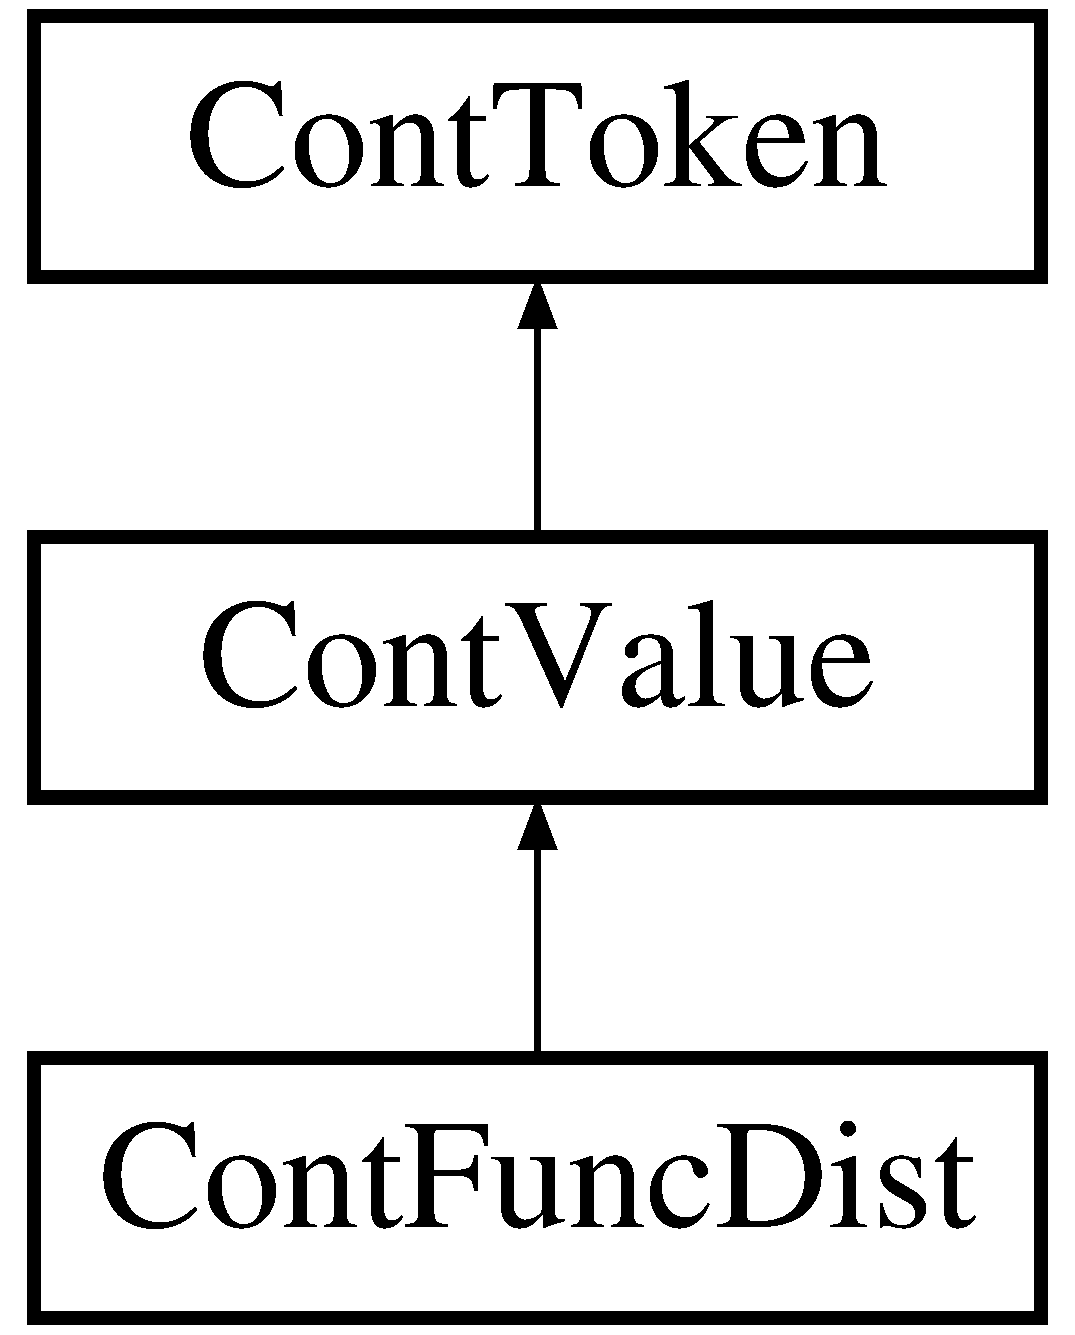
\includegraphics[height=3.000000cm]{a00054}
\end{center}
\end{figure}
\subsection*{Public Member Functions}
\begin{DoxyCompactItemize}
\item 
\hyperlink{a00054_a97706d170a756b8562306a1093b12254}{Cont\-Func\-Dist} (\hyperlink{a00062}{Cont\-Point} $\ast$p)
\item 
virtual \hyperlink{a00054_a1cb1e8eb3fffedcf8eed9c4e34a5718b}{$\sim$\-Cont\-Func\-Dist} ()
\item 
virtual float \hyperlink{a00054_aa331b7ff493f29881399cdc476219d5b}{Get} (\hyperlink{a00007}{Animate\-Compile} $\ast$anim) const 
\end{DoxyCompactItemize}
\subsection*{Private Attributes}
\begin{DoxyCompactItemize}
\item 
\hyperlink{a00062}{Cont\-Point} $\ast$ \hyperlink{a00054_a16341c9754535537ff04e6dc557b1d48}{pnt}
\end{DoxyCompactItemize}
\subsection*{Additional Inherited Members}


\subsection{Constructor \& Destructor Documentation}
\hypertarget{a00054_a97706d170a756b8562306a1093b12254}{\index{Cont\-Func\-Dist@{Cont\-Func\-Dist}!Cont\-Func\-Dist@{Cont\-Func\-Dist}}
\index{Cont\-Func\-Dist@{Cont\-Func\-Dist}!ContFuncDist@{Cont\-Func\-Dist}}
\subsubsection[{Cont\-Func\-Dist}]{\setlength{\rightskip}{0pt plus 5cm}Cont\-Func\-Dist\-::\-Cont\-Func\-Dist (
\begin{DoxyParamCaption}
\item[{{\bf Cont\-Point} $\ast$}]{p}
\end{DoxyParamCaption}
)\hspace{0.3cm}{\ttfamily [inline]}}}\label{a00054_a97706d170a756b8562306a1093b12254}
\hypertarget{a00054_a1cb1e8eb3fffedcf8eed9c4e34a5718b}{\index{Cont\-Func\-Dist@{Cont\-Func\-Dist}!$\sim$\-Cont\-Func\-Dist@{$\sim$\-Cont\-Func\-Dist}}
\index{$\sim$\-Cont\-Func\-Dist@{$\sim$\-Cont\-Func\-Dist}!ContFuncDist@{Cont\-Func\-Dist}}
\subsubsection[{$\sim$\-Cont\-Func\-Dist}]{\setlength{\rightskip}{0pt plus 5cm}Cont\-Func\-Dist\-::$\sim$\-Cont\-Func\-Dist (
\begin{DoxyParamCaption}
{}
\end{DoxyParamCaption}
)\hspace{0.3cm}{\ttfamily [virtual]}}}\label{a00054_a1cb1e8eb3fffedcf8eed9c4e34a5718b}


\subsection{Member Function Documentation}
\hypertarget{a00054_aa331b7ff493f29881399cdc476219d5b}{\index{Cont\-Func\-Dist@{Cont\-Func\-Dist}!Get@{Get}}
\index{Get@{Get}!ContFuncDist@{Cont\-Func\-Dist}}
\subsubsection[{Get}]{\setlength{\rightskip}{0pt plus 5cm}float Cont\-Func\-Dist\-::\-Get (
\begin{DoxyParamCaption}
\item[{{\bf Animate\-Compile} $\ast$}]{anim}
\end{DoxyParamCaption}
) const\hspace{0.3cm}{\ttfamily [virtual]}}}\label{a00054_aa331b7ff493f29881399cdc476219d5b}


Implements \hyperlink{a00086_ae3ce98084899bf1a873a1ec6bf15116e}{Cont\-Value}.



\subsection{Member Data Documentation}
\hypertarget{a00054_a16341c9754535537ff04e6dc557b1d48}{\index{Cont\-Func\-Dist@{Cont\-Func\-Dist}!pnt@{pnt}}
\index{pnt@{pnt}!ContFuncDist@{Cont\-Func\-Dist}}
\subsubsection[{pnt}]{\setlength{\rightskip}{0pt plus 5cm}{\bf Cont\-Point}$\ast$ Cont\-Func\-Dist\-::pnt\hspace{0.3cm}{\ttfamily [private]}}}\label{a00054_a16341c9754535537ff04e6dc557b1d48}


The documentation for this class was generated from the following files\-:\begin{DoxyCompactItemize}
\item 
src/core/\hyperlink{a00218}{cont.\-h}\item 
src/core/\hyperlink{a00217}{cont.\-cpp}\end{DoxyCompactItemize}

\hypertarget{a00055}{\section{Cont\-Func\-Dist\-From Class Reference}
\label{a00055}\index{Cont\-Func\-Dist\-From@{Cont\-Func\-Dist\-From}}
}


{\ttfamily \#include $<$cont.\-h$>$}

Inheritance diagram for Cont\-Func\-Dist\-From\-:\begin{figure}[H]
\begin{center}
\leavevmode
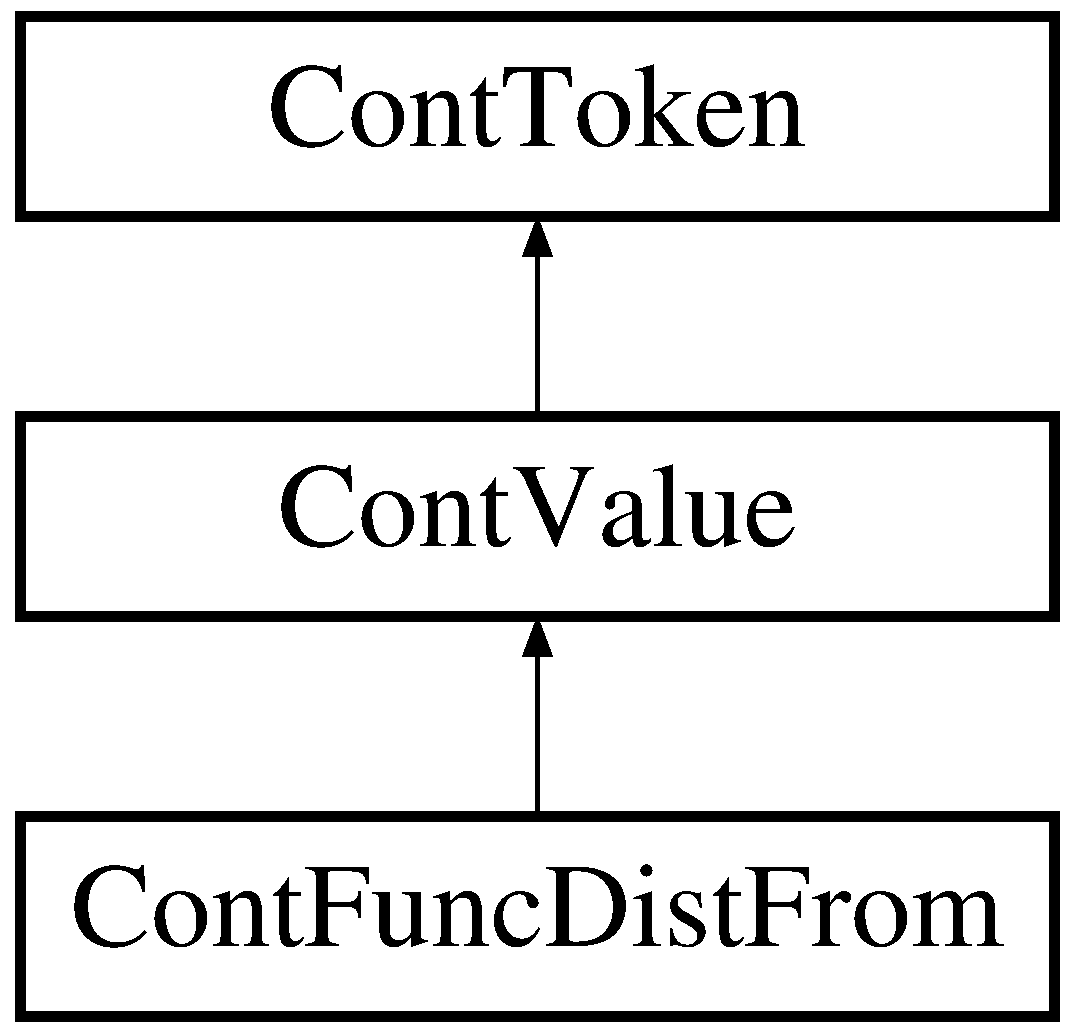
\includegraphics[height=3.000000cm]{a00055}
\end{center}
\end{figure}
\subsection*{Public Member Functions}
\begin{DoxyCompactItemize}
\item 
\hyperlink{a00055_abd7324bac1a52e3bf7b6701d25a8dbcd}{Cont\-Func\-Dist\-From} (\hyperlink{a00062}{Cont\-Point} $\ast$start, \hyperlink{a00062}{Cont\-Point} $\ast$end)
\item 
virtual \hyperlink{a00055_a5658a543adb8b5e1d2ca6c754f2aa271}{$\sim$\-Cont\-Func\-Dist\-From} ()
\item 
virtual float \hyperlink{a00055_a152f3bb0dc7650622079af59b55b4a6c}{Get} (\hyperlink{a00007}{Animate\-Compile} $\ast$anim) const 
\end{DoxyCompactItemize}
\subsection*{Private Attributes}
\begin{DoxyCompactItemize}
\item 
\hyperlink{a00062}{Cont\-Point} $\ast$ \hyperlink{a00055_a25338c27e80b5da31dcfd66fab8301b0}{pnt\-\_\-start}
\item 
\hyperlink{a00062}{Cont\-Point} $\ast$ \hyperlink{a00055_af5ec896aa9096b288b261444c42f0e54}{pnt\-\_\-end}
\end{DoxyCompactItemize}
\subsection*{Additional Inherited Members}


\subsection{Constructor \& Destructor Documentation}
\hypertarget{a00055_abd7324bac1a52e3bf7b6701d25a8dbcd}{\index{Cont\-Func\-Dist\-From@{Cont\-Func\-Dist\-From}!Cont\-Func\-Dist\-From@{Cont\-Func\-Dist\-From}}
\index{Cont\-Func\-Dist\-From@{Cont\-Func\-Dist\-From}!ContFuncDistFrom@{Cont\-Func\-Dist\-From}}
\subsubsection[{Cont\-Func\-Dist\-From}]{\setlength{\rightskip}{0pt plus 5cm}Cont\-Func\-Dist\-From\-::\-Cont\-Func\-Dist\-From (
\begin{DoxyParamCaption}
\item[{{\bf Cont\-Point} $\ast$}]{start, }
\item[{{\bf Cont\-Point} $\ast$}]{end}
\end{DoxyParamCaption}
)\hspace{0.3cm}{\ttfamily [inline]}}}\label{a00055_abd7324bac1a52e3bf7b6701d25a8dbcd}
\hypertarget{a00055_a5658a543adb8b5e1d2ca6c754f2aa271}{\index{Cont\-Func\-Dist\-From@{Cont\-Func\-Dist\-From}!$\sim$\-Cont\-Func\-Dist\-From@{$\sim$\-Cont\-Func\-Dist\-From}}
\index{$\sim$\-Cont\-Func\-Dist\-From@{$\sim$\-Cont\-Func\-Dist\-From}!ContFuncDistFrom@{Cont\-Func\-Dist\-From}}
\subsubsection[{$\sim$\-Cont\-Func\-Dist\-From}]{\setlength{\rightskip}{0pt plus 5cm}Cont\-Func\-Dist\-From\-::$\sim$\-Cont\-Func\-Dist\-From (
\begin{DoxyParamCaption}
{}
\end{DoxyParamCaption}
)\hspace{0.3cm}{\ttfamily [virtual]}}}\label{a00055_a5658a543adb8b5e1d2ca6c754f2aa271}


\subsection{Member Function Documentation}
\hypertarget{a00055_a152f3bb0dc7650622079af59b55b4a6c}{\index{Cont\-Func\-Dist\-From@{Cont\-Func\-Dist\-From}!Get@{Get}}
\index{Get@{Get}!ContFuncDistFrom@{Cont\-Func\-Dist\-From}}
\subsubsection[{Get}]{\setlength{\rightskip}{0pt plus 5cm}float Cont\-Func\-Dist\-From\-::\-Get (
\begin{DoxyParamCaption}
\item[{{\bf Animate\-Compile} $\ast$}]{anim}
\end{DoxyParamCaption}
) const\hspace{0.3cm}{\ttfamily [virtual]}}}\label{a00055_a152f3bb0dc7650622079af59b55b4a6c}


Implements \hyperlink{a00086_ae3ce98084899bf1a873a1ec6bf15116e}{Cont\-Value}.



\subsection{Member Data Documentation}
\hypertarget{a00055_af5ec896aa9096b288b261444c42f0e54}{\index{Cont\-Func\-Dist\-From@{Cont\-Func\-Dist\-From}!pnt\-\_\-end@{pnt\-\_\-end}}
\index{pnt\-\_\-end@{pnt\-\_\-end}!ContFuncDistFrom@{Cont\-Func\-Dist\-From}}
\subsubsection[{pnt\-\_\-end}]{\setlength{\rightskip}{0pt plus 5cm}{\bf Cont\-Point} $\ast$ Cont\-Func\-Dist\-From\-::pnt\-\_\-end\hspace{0.3cm}{\ttfamily [private]}}}\label{a00055_af5ec896aa9096b288b261444c42f0e54}
\hypertarget{a00055_a25338c27e80b5da31dcfd66fab8301b0}{\index{Cont\-Func\-Dist\-From@{Cont\-Func\-Dist\-From}!pnt\-\_\-start@{pnt\-\_\-start}}
\index{pnt\-\_\-start@{pnt\-\_\-start}!ContFuncDistFrom@{Cont\-Func\-Dist\-From}}
\subsubsection[{pnt\-\_\-start}]{\setlength{\rightskip}{0pt plus 5cm}{\bf Cont\-Point}$\ast$ Cont\-Func\-Dist\-From\-::pnt\-\_\-start\hspace{0.3cm}{\ttfamily [private]}}}\label{a00055_a25338c27e80b5da31dcfd66fab8301b0}


The documentation for this class was generated from the following files\-:\begin{DoxyCompactItemize}
\item 
src/core/\hyperlink{a00218}{cont.\-h}\item 
src/core/\hyperlink{a00217}{cont.\-cpp}\end{DoxyCompactItemize}

\hypertarget{a00056}{\section{Cont\-Func\-Either Class Reference}
\label{a00056}\index{Cont\-Func\-Either@{Cont\-Func\-Either}}
}


{\ttfamily \#include $<$cont.\-h$>$}

Inheritance diagram for Cont\-Func\-Either\-:\begin{figure}[H]
\begin{center}
\leavevmode
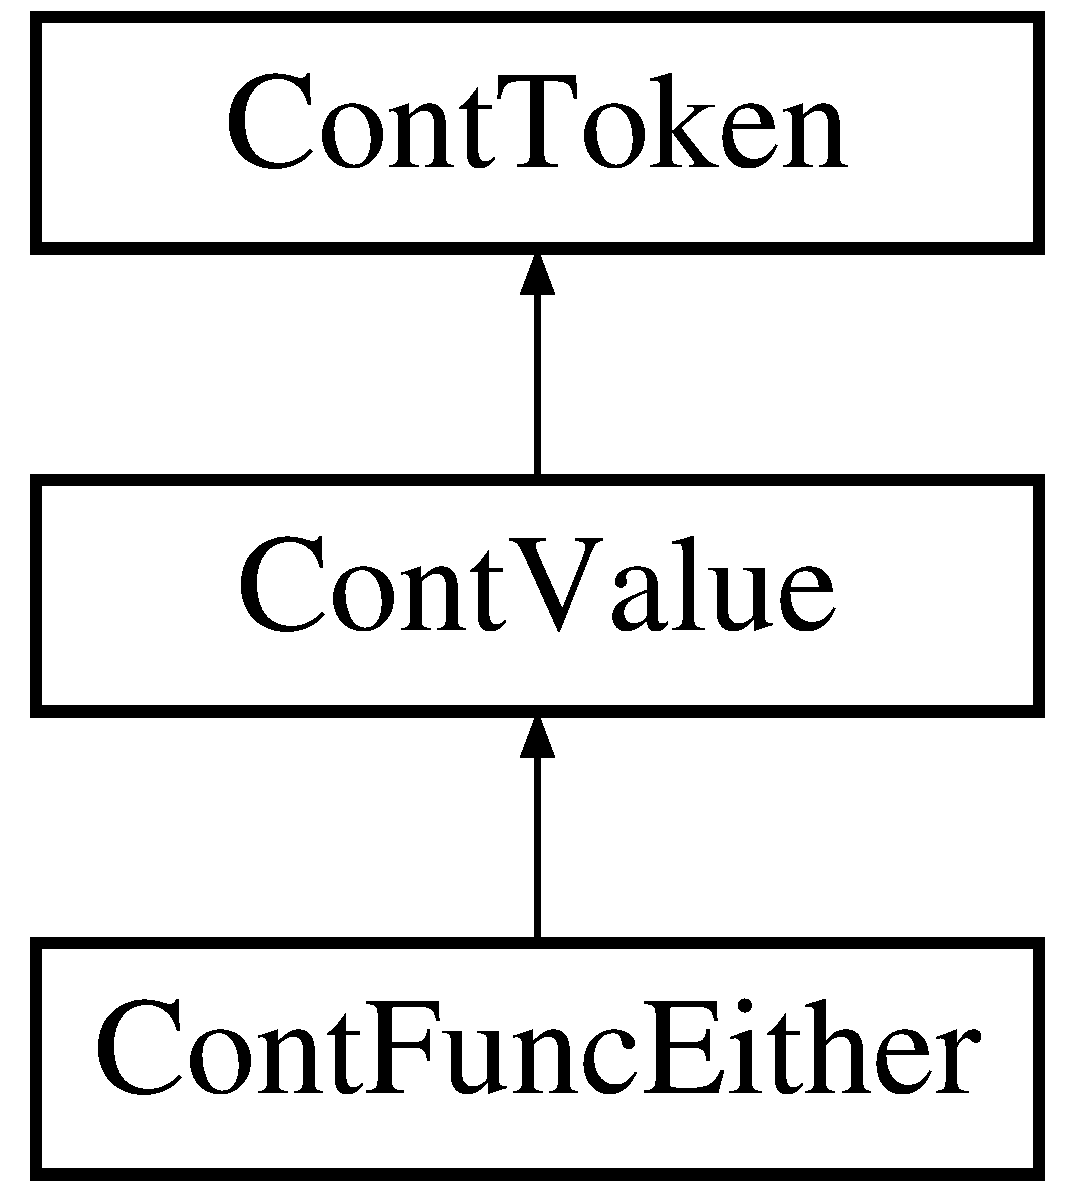
\includegraphics[height=3.000000cm]{a00056}
\end{center}
\end{figure}
\subsection*{Public Member Functions}
\begin{DoxyCompactItemize}
\item 
\hyperlink{a00056_abb1aa4e2ca328032e00da37314bd6104}{Cont\-Func\-Either} (\hyperlink{a00086}{Cont\-Value} $\ast$d1, \hyperlink{a00086}{Cont\-Value} $\ast$d2, \hyperlink{a00062}{Cont\-Point} $\ast$p)
\item 
virtual \hyperlink{a00056_af85381508aea6c81e26cc73aabb2846b}{$\sim$\-Cont\-Func\-Either} ()
\item 
virtual float \hyperlink{a00056_af0ef72e3cbf2d0fc95e834f552e138ce}{Get} (\hyperlink{a00007}{Animate\-Compile} $\ast$anim) const 
\end{DoxyCompactItemize}
\subsection*{Private Attributes}
\begin{DoxyCompactItemize}
\item 
\hyperlink{a00086}{Cont\-Value} $\ast$ \hyperlink{a00056_a34dc3d7f09ab0d1eeba98592e2b1ca71}{dir1}
\item 
\hyperlink{a00086}{Cont\-Value} $\ast$ \hyperlink{a00056_affc948c83c590f610d5c02230237d7fa}{dir2}
\item 
\hyperlink{a00062}{Cont\-Point} $\ast$ \hyperlink{a00056_a04b8c169797d08e1bbf9d21ecc1ec6d2}{pnt}
\end{DoxyCompactItemize}
\subsection*{Additional Inherited Members}


\subsection{Constructor \& Destructor Documentation}
\hypertarget{a00056_abb1aa4e2ca328032e00da37314bd6104}{\index{Cont\-Func\-Either@{Cont\-Func\-Either}!Cont\-Func\-Either@{Cont\-Func\-Either}}
\index{Cont\-Func\-Either@{Cont\-Func\-Either}!ContFuncEither@{Cont\-Func\-Either}}
\subsubsection[{Cont\-Func\-Either}]{\setlength{\rightskip}{0pt plus 5cm}Cont\-Func\-Either\-::\-Cont\-Func\-Either (
\begin{DoxyParamCaption}
\item[{{\bf Cont\-Value} $\ast$}]{d1, }
\item[{{\bf Cont\-Value} $\ast$}]{d2, }
\item[{{\bf Cont\-Point} $\ast$}]{p}
\end{DoxyParamCaption}
)\hspace{0.3cm}{\ttfamily [inline]}}}\label{a00056_abb1aa4e2ca328032e00da37314bd6104}
\hypertarget{a00056_af85381508aea6c81e26cc73aabb2846b}{\index{Cont\-Func\-Either@{Cont\-Func\-Either}!$\sim$\-Cont\-Func\-Either@{$\sim$\-Cont\-Func\-Either}}
\index{$\sim$\-Cont\-Func\-Either@{$\sim$\-Cont\-Func\-Either}!ContFuncEither@{Cont\-Func\-Either}}
\subsubsection[{$\sim$\-Cont\-Func\-Either}]{\setlength{\rightskip}{0pt plus 5cm}Cont\-Func\-Either\-::$\sim$\-Cont\-Func\-Either (
\begin{DoxyParamCaption}
{}
\end{DoxyParamCaption}
)\hspace{0.3cm}{\ttfamily [virtual]}}}\label{a00056_af85381508aea6c81e26cc73aabb2846b}


\subsection{Member Function Documentation}
\hypertarget{a00056_af0ef72e3cbf2d0fc95e834f552e138ce}{\index{Cont\-Func\-Either@{Cont\-Func\-Either}!Get@{Get}}
\index{Get@{Get}!ContFuncEither@{Cont\-Func\-Either}}
\subsubsection[{Get}]{\setlength{\rightskip}{0pt plus 5cm}float Cont\-Func\-Either\-::\-Get (
\begin{DoxyParamCaption}
\item[{{\bf Animate\-Compile} $\ast$}]{anim}
\end{DoxyParamCaption}
) const\hspace{0.3cm}{\ttfamily [virtual]}}}\label{a00056_af0ef72e3cbf2d0fc95e834f552e138ce}


Implements \hyperlink{a00086_ae3ce98084899bf1a873a1ec6bf15116e}{Cont\-Value}.



\subsection{Member Data Documentation}
\hypertarget{a00056_a34dc3d7f09ab0d1eeba98592e2b1ca71}{\index{Cont\-Func\-Either@{Cont\-Func\-Either}!dir1@{dir1}}
\index{dir1@{dir1}!ContFuncEither@{Cont\-Func\-Either}}
\subsubsection[{dir1}]{\setlength{\rightskip}{0pt plus 5cm}{\bf Cont\-Value}$\ast$ Cont\-Func\-Either\-::dir1\hspace{0.3cm}{\ttfamily [private]}}}\label{a00056_a34dc3d7f09ab0d1eeba98592e2b1ca71}
\hypertarget{a00056_affc948c83c590f610d5c02230237d7fa}{\index{Cont\-Func\-Either@{Cont\-Func\-Either}!dir2@{dir2}}
\index{dir2@{dir2}!ContFuncEither@{Cont\-Func\-Either}}
\subsubsection[{dir2}]{\setlength{\rightskip}{0pt plus 5cm}{\bf Cont\-Value} $\ast$ Cont\-Func\-Either\-::dir2\hspace{0.3cm}{\ttfamily [private]}}}\label{a00056_affc948c83c590f610d5c02230237d7fa}
\hypertarget{a00056_a04b8c169797d08e1bbf9d21ecc1ec6d2}{\index{Cont\-Func\-Either@{Cont\-Func\-Either}!pnt@{pnt}}
\index{pnt@{pnt}!ContFuncEither@{Cont\-Func\-Either}}
\subsubsection[{pnt}]{\setlength{\rightskip}{0pt plus 5cm}{\bf Cont\-Point}$\ast$ Cont\-Func\-Either\-::pnt\hspace{0.3cm}{\ttfamily [private]}}}\label{a00056_a04b8c169797d08e1bbf9d21ecc1ec6d2}


The documentation for this class was generated from the following files\-:\begin{DoxyCompactItemize}
\item 
src/core/\hyperlink{a00218}{cont.\-h}\item 
src/core/\hyperlink{a00217}{cont.\-cpp}\end{DoxyCompactItemize}

\hypertarget{a00057}{\section{Cont\-Func\-Opp Class Reference}
\label{a00057}\index{Cont\-Func\-Opp@{Cont\-Func\-Opp}}
}


{\ttfamily \#include $<$cont.\-h$>$}

Inheritance diagram for Cont\-Func\-Opp\-:\begin{figure}[H]
\begin{center}
\leavevmode
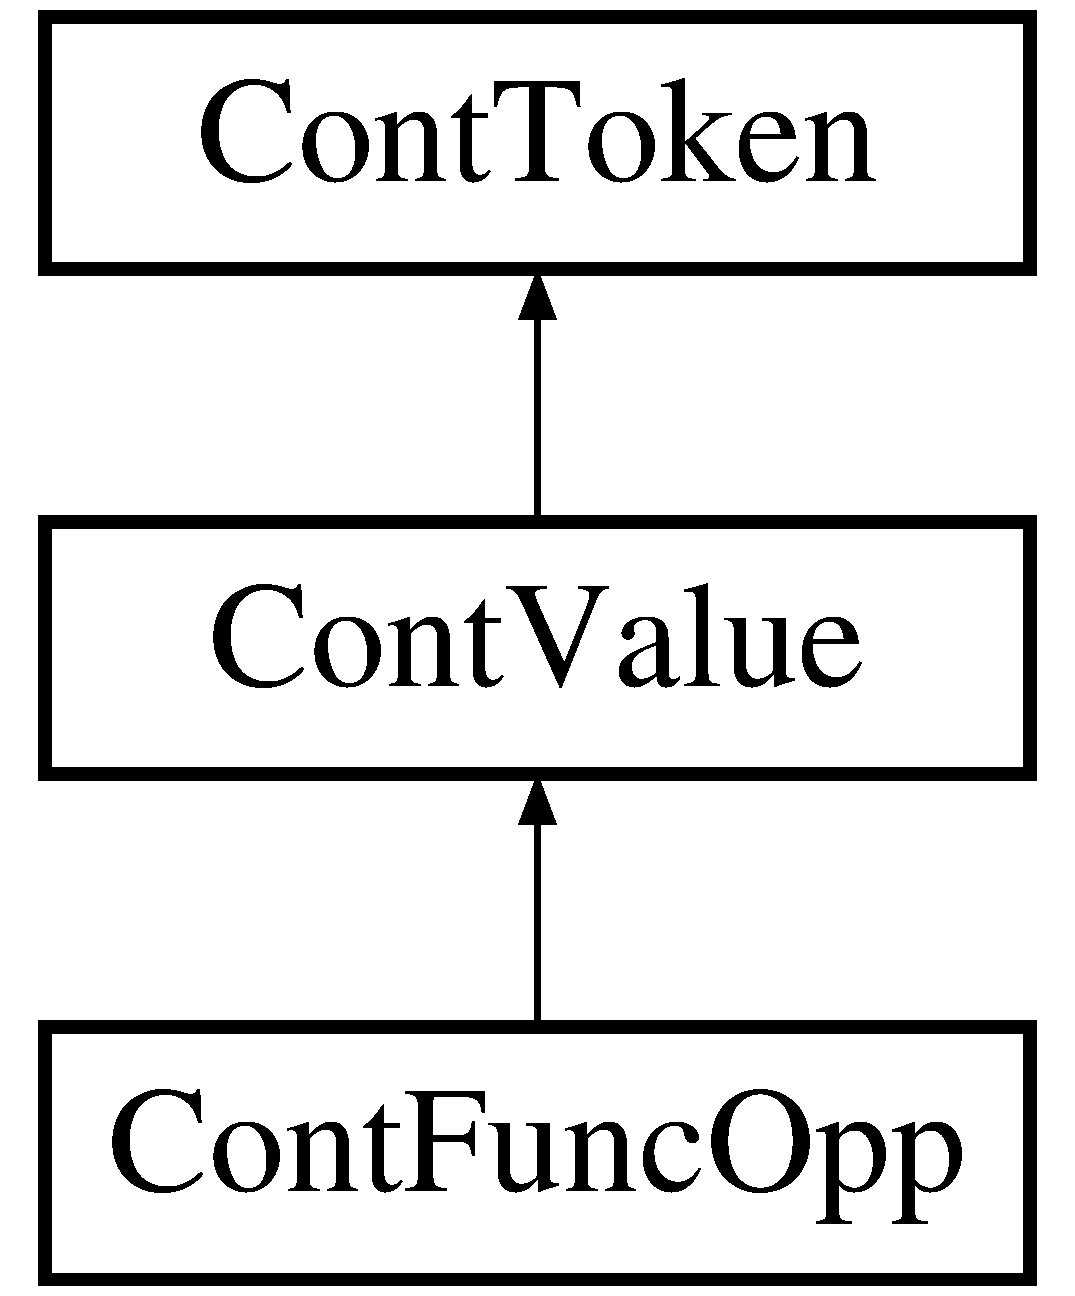
\includegraphics[height=3.000000cm]{a00057}
\end{center}
\end{figure}
\subsection*{Public Member Functions}
\begin{DoxyCompactItemize}
\item 
\hyperlink{a00057_a85b475a28af7b4af6c36880bce631cd5}{Cont\-Func\-Opp} (\hyperlink{a00086}{Cont\-Value} $\ast$d)
\item 
virtual \hyperlink{a00057_a4796c527230cbd0a04ecf252638db445}{$\sim$\-Cont\-Func\-Opp} ()
\item 
virtual float \hyperlink{a00057_adb4821819f197ecb965b7254660652e3}{Get} (\hyperlink{a00007}{Animate\-Compile} $\ast$anim) const 
\end{DoxyCompactItemize}
\subsection*{Private Attributes}
\begin{DoxyCompactItemize}
\item 
\hyperlink{a00086}{Cont\-Value} $\ast$ \hyperlink{a00057_ae5a5be8f69b24e66e27c07368ada1024}{dir}
\end{DoxyCompactItemize}
\subsection*{Additional Inherited Members}


\subsection{Constructor \& Destructor Documentation}
\hypertarget{a00057_a85b475a28af7b4af6c36880bce631cd5}{\index{Cont\-Func\-Opp@{Cont\-Func\-Opp}!Cont\-Func\-Opp@{Cont\-Func\-Opp}}
\index{Cont\-Func\-Opp@{Cont\-Func\-Opp}!ContFuncOpp@{Cont\-Func\-Opp}}
\subsubsection[{Cont\-Func\-Opp}]{\setlength{\rightskip}{0pt plus 5cm}Cont\-Func\-Opp\-::\-Cont\-Func\-Opp (
\begin{DoxyParamCaption}
\item[{{\bf Cont\-Value} $\ast$}]{d}
\end{DoxyParamCaption}
)\hspace{0.3cm}{\ttfamily [inline]}}}\label{a00057_a85b475a28af7b4af6c36880bce631cd5}
\hypertarget{a00057_a4796c527230cbd0a04ecf252638db445}{\index{Cont\-Func\-Opp@{Cont\-Func\-Opp}!$\sim$\-Cont\-Func\-Opp@{$\sim$\-Cont\-Func\-Opp}}
\index{$\sim$\-Cont\-Func\-Opp@{$\sim$\-Cont\-Func\-Opp}!ContFuncOpp@{Cont\-Func\-Opp}}
\subsubsection[{$\sim$\-Cont\-Func\-Opp}]{\setlength{\rightskip}{0pt plus 5cm}Cont\-Func\-Opp\-::$\sim$\-Cont\-Func\-Opp (
\begin{DoxyParamCaption}
{}
\end{DoxyParamCaption}
)\hspace{0.3cm}{\ttfamily [virtual]}}}\label{a00057_a4796c527230cbd0a04ecf252638db445}


\subsection{Member Function Documentation}
\hypertarget{a00057_adb4821819f197ecb965b7254660652e3}{\index{Cont\-Func\-Opp@{Cont\-Func\-Opp}!Get@{Get}}
\index{Get@{Get}!ContFuncOpp@{Cont\-Func\-Opp}}
\subsubsection[{Get}]{\setlength{\rightskip}{0pt plus 5cm}float Cont\-Func\-Opp\-::\-Get (
\begin{DoxyParamCaption}
\item[{{\bf Animate\-Compile} $\ast$}]{anim}
\end{DoxyParamCaption}
) const\hspace{0.3cm}{\ttfamily [virtual]}}}\label{a00057_adb4821819f197ecb965b7254660652e3}


Implements \hyperlink{a00086_ae3ce98084899bf1a873a1ec6bf15116e}{Cont\-Value}.



\subsection{Member Data Documentation}
\hypertarget{a00057_ae5a5be8f69b24e66e27c07368ada1024}{\index{Cont\-Func\-Opp@{Cont\-Func\-Opp}!dir@{dir}}
\index{dir@{dir}!ContFuncOpp@{Cont\-Func\-Opp}}
\subsubsection[{dir}]{\setlength{\rightskip}{0pt plus 5cm}{\bf Cont\-Value}$\ast$ Cont\-Func\-Opp\-::dir\hspace{0.3cm}{\ttfamily [private]}}}\label{a00057_ae5a5be8f69b24e66e27c07368ada1024}


The documentation for this class was generated from the following files\-:\begin{DoxyCompactItemize}
\item 
src/core/\hyperlink{a00218}{cont.\-h}\item 
src/core/\hyperlink{a00217}{cont.\-cpp}\end{DoxyCompactItemize}

\hypertarget{a00058}{\section{Cont\-Func\-Step Class Reference}
\label{a00058}\index{Cont\-Func\-Step@{Cont\-Func\-Step}}
}


{\ttfamily \#include $<$cont.\-h$>$}

Inheritance diagram for Cont\-Func\-Step\-:\begin{figure}[H]
\begin{center}
\leavevmode
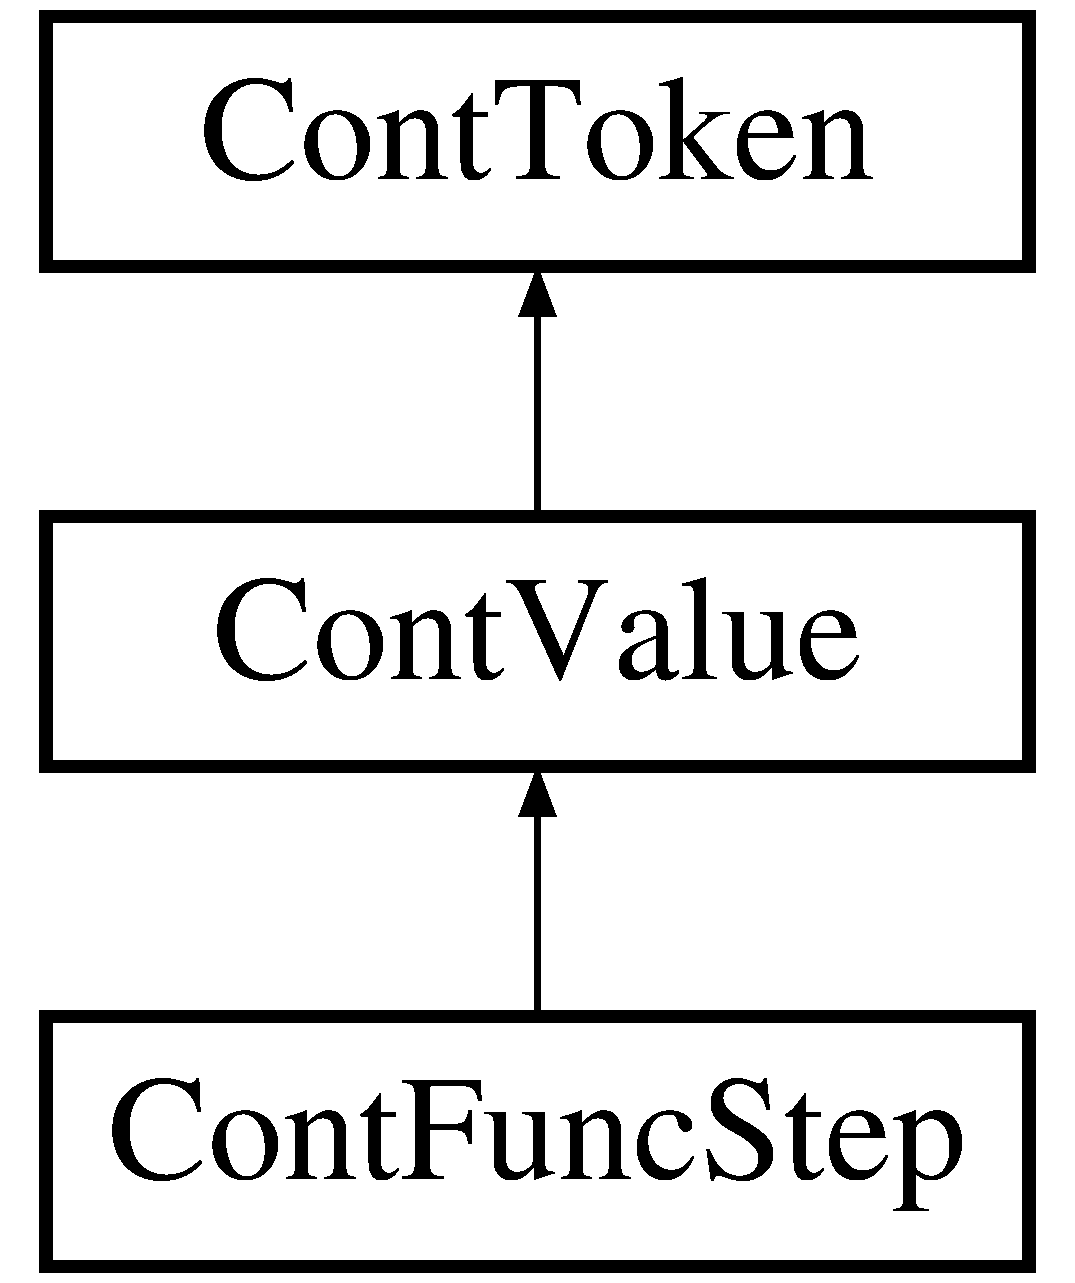
\includegraphics[height=3.000000cm]{a00058}
\end{center}
\end{figure}
\subsection*{Public Member Functions}
\begin{DoxyCompactItemize}
\item 
\hyperlink{a00058_aadda36c5a5639224ce73bc88d9a67b77}{Cont\-Func\-Step} (\hyperlink{a00086}{Cont\-Value} $\ast$beats, \hyperlink{a00086}{Cont\-Value} $\ast$blocksize, \hyperlink{a00062}{Cont\-Point} $\ast$p)
\item 
virtual \hyperlink{a00058_a994c24500c38f1c1cb9426313a7270e8}{$\sim$\-Cont\-Func\-Step} ()
\item 
virtual float \hyperlink{a00058_a77931d7840c6fa3a948bf40b16633598}{Get} (\hyperlink{a00007}{Animate\-Compile} $\ast$anim) const 
\end{DoxyCompactItemize}
\subsection*{Private Attributes}
\begin{DoxyCompactItemize}
\item 
\hyperlink{a00086}{Cont\-Value} $\ast$ \hyperlink{a00058_a5695048b68de893beacc7ade45d483a6}{numbeats}
\item 
\hyperlink{a00086}{Cont\-Value} $\ast$ \hyperlink{a00058_a5c9588cbcc73f026ad1f393717b23dd7}{blksize}
\item 
\hyperlink{a00062}{Cont\-Point} $\ast$ \hyperlink{a00058_ad5525f949ad5b9c94ce3d242f44fef54}{pnt}
\end{DoxyCompactItemize}
\subsection*{Additional Inherited Members}


\subsection{Constructor \& Destructor Documentation}
\hypertarget{a00058_aadda36c5a5639224ce73bc88d9a67b77}{\index{Cont\-Func\-Step@{Cont\-Func\-Step}!Cont\-Func\-Step@{Cont\-Func\-Step}}
\index{Cont\-Func\-Step@{Cont\-Func\-Step}!ContFuncStep@{Cont\-Func\-Step}}
\subsubsection[{Cont\-Func\-Step}]{\setlength{\rightskip}{0pt plus 5cm}Cont\-Func\-Step\-::\-Cont\-Func\-Step (
\begin{DoxyParamCaption}
\item[{{\bf Cont\-Value} $\ast$}]{beats, }
\item[{{\bf Cont\-Value} $\ast$}]{blocksize, }
\item[{{\bf Cont\-Point} $\ast$}]{p}
\end{DoxyParamCaption}
)\hspace{0.3cm}{\ttfamily [inline]}}}\label{a00058_aadda36c5a5639224ce73bc88d9a67b77}
\hypertarget{a00058_a994c24500c38f1c1cb9426313a7270e8}{\index{Cont\-Func\-Step@{Cont\-Func\-Step}!$\sim$\-Cont\-Func\-Step@{$\sim$\-Cont\-Func\-Step}}
\index{$\sim$\-Cont\-Func\-Step@{$\sim$\-Cont\-Func\-Step}!ContFuncStep@{Cont\-Func\-Step}}
\subsubsection[{$\sim$\-Cont\-Func\-Step}]{\setlength{\rightskip}{0pt plus 5cm}Cont\-Func\-Step\-::$\sim$\-Cont\-Func\-Step (
\begin{DoxyParamCaption}
{}
\end{DoxyParamCaption}
)\hspace{0.3cm}{\ttfamily [virtual]}}}\label{a00058_a994c24500c38f1c1cb9426313a7270e8}


\subsection{Member Function Documentation}
\hypertarget{a00058_a77931d7840c6fa3a948bf40b16633598}{\index{Cont\-Func\-Step@{Cont\-Func\-Step}!Get@{Get}}
\index{Get@{Get}!ContFuncStep@{Cont\-Func\-Step}}
\subsubsection[{Get}]{\setlength{\rightskip}{0pt plus 5cm}float Cont\-Func\-Step\-::\-Get (
\begin{DoxyParamCaption}
\item[{{\bf Animate\-Compile} $\ast$}]{anim}
\end{DoxyParamCaption}
) const\hspace{0.3cm}{\ttfamily [virtual]}}}\label{a00058_a77931d7840c6fa3a948bf40b16633598}


Implements \hyperlink{a00086_ae3ce98084899bf1a873a1ec6bf15116e}{Cont\-Value}.



\subsection{Member Data Documentation}
\hypertarget{a00058_a5c9588cbcc73f026ad1f393717b23dd7}{\index{Cont\-Func\-Step@{Cont\-Func\-Step}!blksize@{blksize}}
\index{blksize@{blksize}!ContFuncStep@{Cont\-Func\-Step}}
\subsubsection[{blksize}]{\setlength{\rightskip}{0pt plus 5cm}{\bf Cont\-Value} $\ast$ Cont\-Func\-Step\-::blksize\hspace{0.3cm}{\ttfamily [private]}}}\label{a00058_a5c9588cbcc73f026ad1f393717b23dd7}
\hypertarget{a00058_a5695048b68de893beacc7ade45d483a6}{\index{Cont\-Func\-Step@{Cont\-Func\-Step}!numbeats@{numbeats}}
\index{numbeats@{numbeats}!ContFuncStep@{Cont\-Func\-Step}}
\subsubsection[{numbeats}]{\setlength{\rightskip}{0pt plus 5cm}{\bf Cont\-Value}$\ast$ Cont\-Func\-Step\-::numbeats\hspace{0.3cm}{\ttfamily [private]}}}\label{a00058_a5695048b68de893beacc7ade45d483a6}
\hypertarget{a00058_ad5525f949ad5b9c94ce3d242f44fef54}{\index{Cont\-Func\-Step@{Cont\-Func\-Step}!pnt@{pnt}}
\index{pnt@{pnt}!ContFuncStep@{Cont\-Func\-Step}}
\subsubsection[{pnt}]{\setlength{\rightskip}{0pt plus 5cm}{\bf Cont\-Point}$\ast$ Cont\-Func\-Step\-::pnt\hspace{0.3cm}{\ttfamily [private]}}}\label{a00058_ad5525f949ad5b9c94ce3d242f44fef54}


The documentation for this class was generated from the following files\-:\begin{DoxyCompactItemize}
\item 
src/core/\hyperlink{a00218}{cont.\-h}\item 
src/core/\hyperlink{a00217}{cont.\-cpp}\end{DoxyCompactItemize}

\hypertarget{a00059}{\section{Continuity\-Editor Class Reference}
\label{a00059}\index{Continuity\-Editor@{Continuity\-Editor}}
}


{\ttfamily \#include $<$cont\-\_\-ui.\-h$>$}

Inheritance diagram for Continuity\-Editor\-:\begin{figure}[H]
\begin{center}
\leavevmode
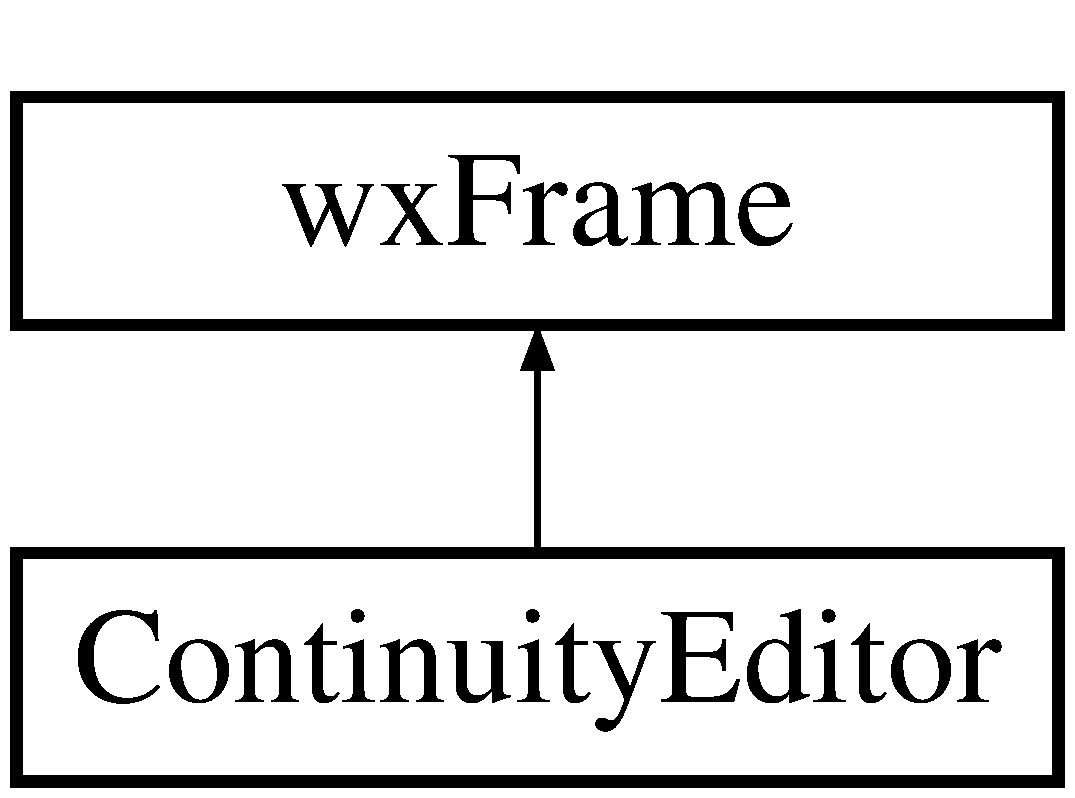
\includegraphics[height=2.000000cm]{a00059}
\end{center}
\end{figure}
\subsection*{Public Member Functions}
\begin{DoxyCompactItemize}
\item 
\hyperlink{a00059_a9e31a8ab139a1b747297d57c7a49c2cc}{Continuity\-Editor} ()
\item 
\hyperlink{a00059_ad60b959f500e59ff49bd1c5b848b5ba5}{Continuity\-Editor} (\hyperlink{a00020}{Cal\-Chart\-Doc} $\ast$dcr, wx\-Window $\ast$parent, wx\-Window\-I\-D id=wx\-I\-D\-\_\-\-A\-N\-Y, const wx\-String \&caption=wx\-T(\char`\"{}Edit Continuity\char`\"{}), const wx\-Point \&pos=wx\-Default\-Position, const wx\-Size \&size=wx\-Default\-Size, long style=wx\-C\-A\-P\-T\-I\-O\-N$\vert$wx\-R\-E\-S\-I\-Z\-E\-\_\-\-B\-O\-R\-D\-E\-R$\vert$wx\-S\-Y\-S\-T\-E\-M\-\_\-\-M\-E\-N\-U)
\item 
\hyperlink{a00059_a3aedb1177617586468e9060f4a4f61bd}{$\sim$\-Continuity\-Editor} ()
\item 
void \hyperlink{a00059_ae6b1600a094778ea4cad6ec5762d8ccf}{On\-Close\-Window} (wx\-Command\-Event \&event)
\item 
void \hyperlink{a00059_a246d7c68af529d577fc454a02500bec6}{On\-Cmd\-Help} (wx\-Command\-Event \&event)
\item 
void \hyperlink{a00059_aa15472d864ce0b5d3be618ae239a85f4}{Update} ()
\item 
void \hyperlink{a00059_adf2bf1ae2342f2ad0f8232c945224865}{Update\-Text} ()
\item 
void \hyperlink{a00059_aa464eca3687ea58cd2e4accec5b6eb1a}{Flush\-Text} ()
\item 
void \hyperlink{a00059_a4ec0afdacc48ad2c794562857f69f803}{Set\-Insertion\-Point} (int x, int y)
\end{DoxyCompactItemize}
\subsection*{Private Member Functions}
\begin{DoxyCompactItemize}
\item 
void \hyperlink{a00059_a046c2c5b4d6d519c2811a41d6cfa2018}{Init} ()
\item 
bool \hyperlink{a00059_a4d9b952ecad906a4b24a3493eb1b83e8}{Create} (\hyperlink{a00020}{Cal\-Chart\-Doc} $\ast$shw, wx\-Window $\ast$parent, wx\-Window\-I\-D id=wx\-I\-D\-\_\-\-A\-N\-Y, const wx\-String \&caption=wx\-T(\char`\"{}Select Points\char`\"{}), const wx\-Point \&pos=wx\-Default\-Position, const wx\-Size \&size=wx\-Default\-Size, long style=wx\-C\-A\-P\-T\-I\-O\-N$\vert$wx\-R\-E\-S\-I\-Z\-E\-\_\-\-B\-O\-R\-D\-E\-R$\vert$wx\-S\-Y\-S\-T\-E\-M\-\_\-\-M\-E\-N\-U)
\item 
void \hyperlink{a00059_a277a8b6213a1ea0dedaa9b0b701613d9}{Create\-Controls} ()
\item 
void \hyperlink{a00059_a173b4eea37a40309145a129b7666909d}{Cont\-Edit\-Set} (wx\-Command\-Event \&)
\item 
void \hyperlink{a00059_a97a7d45a43b24a4eec9f3796e8ebbbd1}{Cont\-Edit\-Select} (wx\-Command\-Event \&)
\item 
void \hyperlink{a00059_aacfbd278347c63ba806eeced2c051dfb}{On\-Save} (wx\-Command\-Event \&)
\item 
void \hyperlink{a00059_a28ef367f2af187994960d346cc991152}{On\-Discard} (wx\-Command\-Event \&)
\item 
void \hyperlink{a00059_a6b22c9739450684689e48c92eddd93b5}{Cont\-Edit\-Current} (wx\-Command\-Event \&)
\item 
void \hyperlink{a00059_adaa335a4925f6d8ba9bfebe80ae6cc36}{On\-Key\-Press} (wx\-Command\-Event \&)
\item 
\hyperlink{a00216_a68cd84e0300be6f9ff4474682762c9ee}{S\-Y\-M\-B\-O\-L\-\_\-\-T\-Y\-P\-E} \hyperlink{a00059_a0604bd21efd58dd298f54c0412898365}{Current\-Symbol\-Choice} () const 
\item 
void \hyperlink{a00059_a068d75aa1d57737882501a34270657d5}{Save} ()
\item 
void \hyperlink{a00059_a64b741dae068c854b2710276a5499439}{Discard} ()
\item 
void \hyperlink{a00059_a708298892b3902a194c27ff5c2d25656}{Set\-Current} (unsigned i)
\end{DoxyCompactItemize}
\subsection*{Private Attributes}
\begin{DoxyCompactItemize}
\item 
\hyperlink{a00020}{Cal\-Chart\-Doc} $\ast$ \hyperlink{a00059_a9df4640d3225da11c158d3ae43919383}{m\-Doc}
\item 
\hyperlink{a00060}{Continuity\-Editor\-View} $\ast$ \hyperlink{a00059_a8ad7327450c133c44597a8118ffb763d}{m\-View}
\item 
wx\-Choice $\ast$ \hyperlink{a00059_ab4ab21c86c7773f0bb18f950a65a3acc}{m\-Continuity\-Choices}
\item 
unsigned \hyperlink{a00059_a1aac5b2bb163261ad3b9282a259de30f}{m\-Current\-Continuity\-Choice}
\item 
\hyperlink{a00099}{Fancy\-Text\-Win} $\ast$ \hyperlink{a00059_a31dc18431e666579860cadbffd361617}{m\-User\-Input}
\item 
\hyperlink{a00046_aaaf1345012d2f833d1c8f28f9b8593ff}{C\-C\-\_\-show\-::const\-\_\-\-C\-C\-\_\-sheet\-\_\-iterator\-\_\-t} \hyperlink{a00059_a3da0ebb4353b7676a0e1423048f775b9}{m\-Sheet\-Under\-Edit}
\end{DoxyCompactItemize}
\subsection*{Friends}
\begin{DoxyCompactItemize}
\item 
class \hyperlink{a00059_a104d1ac9772fb7de9d6d97f14589005a}{Continuity\-Editor\-View}
\end{DoxyCompactItemize}


\subsection{Constructor \& Destructor Documentation}
\hypertarget{a00059_a9e31a8ab139a1b747297d57c7a49c2cc}{\index{Continuity\-Editor@{Continuity\-Editor}!Continuity\-Editor@{Continuity\-Editor}}
\index{Continuity\-Editor@{Continuity\-Editor}!ContinuityEditor@{Continuity\-Editor}}
\subsubsection[{Continuity\-Editor}]{\setlength{\rightskip}{0pt plus 5cm}Continuity\-Editor\-::\-Continuity\-Editor (
\begin{DoxyParamCaption}
{}
\end{DoxyParamCaption}
)}}\label{a00059_a9e31a8ab139a1b747297d57c7a49c2cc}
\hypertarget{a00059_ad60b959f500e59ff49bd1c5b848b5ba5}{\index{Continuity\-Editor@{Continuity\-Editor}!Continuity\-Editor@{Continuity\-Editor}}
\index{Continuity\-Editor@{Continuity\-Editor}!ContinuityEditor@{Continuity\-Editor}}
\subsubsection[{Continuity\-Editor}]{\setlength{\rightskip}{0pt plus 5cm}Continuity\-Editor\-::\-Continuity\-Editor (
\begin{DoxyParamCaption}
\item[{{\bf Cal\-Chart\-Doc} $\ast$}]{dcr, }
\item[{wx\-Window $\ast$}]{parent, }
\item[{wx\-Window\-I\-D}]{id = {\ttfamily wxID\-\_\-ANY}, }
\item[{const wx\-String \&}]{caption = {\ttfamily wxT(\char`\"{}Edit~Continuity\char`\"{})}, }
\item[{const wx\-Point \&}]{pos = {\ttfamily wxDefaultPosition}, }
\item[{const wx\-Size \&}]{size = {\ttfamily wxDefaultSize}, }
\item[{long}]{style = {\ttfamily wxCAPTION$\vert$wxRESIZE\-\_\-BORDER$\vert$wxSYSTEM\-\_\-MENU}}
\end{DoxyParamCaption}
)}}\label{a00059_ad60b959f500e59ff49bd1c5b848b5ba5}
\hypertarget{a00059_a3aedb1177617586468e9060f4a4f61bd}{\index{Continuity\-Editor@{Continuity\-Editor}!$\sim$\-Continuity\-Editor@{$\sim$\-Continuity\-Editor}}
\index{$\sim$\-Continuity\-Editor@{$\sim$\-Continuity\-Editor}!ContinuityEditor@{Continuity\-Editor}}
\subsubsection[{$\sim$\-Continuity\-Editor}]{\setlength{\rightskip}{0pt plus 5cm}Continuity\-Editor\-::$\sim$\-Continuity\-Editor (
\begin{DoxyParamCaption}
{}
\end{DoxyParamCaption}
)}}\label{a00059_a3aedb1177617586468e9060f4a4f61bd}


\subsection{Member Function Documentation}
\hypertarget{a00059_a6b22c9739450684689e48c92eddd93b5}{\index{Continuity\-Editor@{Continuity\-Editor}!Cont\-Edit\-Current@{Cont\-Edit\-Current}}
\index{Cont\-Edit\-Current@{Cont\-Edit\-Current}!ContinuityEditor@{Continuity\-Editor}}
\subsubsection[{Cont\-Edit\-Current}]{\setlength{\rightskip}{0pt plus 5cm}void Continuity\-Editor\-::\-Cont\-Edit\-Current (
\begin{DoxyParamCaption}
\item[{wx\-Command\-Event \&}]{}
\end{DoxyParamCaption}
)\hspace{0.3cm}{\ttfamily [private]}}}\label{a00059_a6b22c9739450684689e48c92eddd93b5}
\hypertarget{a00059_a97a7d45a43b24a4eec9f3796e8ebbbd1}{\index{Continuity\-Editor@{Continuity\-Editor}!Cont\-Edit\-Select@{Cont\-Edit\-Select}}
\index{Cont\-Edit\-Select@{Cont\-Edit\-Select}!ContinuityEditor@{Continuity\-Editor}}
\subsubsection[{Cont\-Edit\-Select}]{\setlength{\rightskip}{0pt plus 5cm}void Continuity\-Editor\-::\-Cont\-Edit\-Select (
\begin{DoxyParamCaption}
\item[{wx\-Command\-Event \&}]{}
\end{DoxyParamCaption}
)\hspace{0.3cm}{\ttfamily [private]}}}\label{a00059_a97a7d45a43b24a4eec9f3796e8ebbbd1}
\hypertarget{a00059_a173b4eea37a40309145a129b7666909d}{\index{Continuity\-Editor@{Continuity\-Editor}!Cont\-Edit\-Set@{Cont\-Edit\-Set}}
\index{Cont\-Edit\-Set@{Cont\-Edit\-Set}!ContinuityEditor@{Continuity\-Editor}}
\subsubsection[{Cont\-Edit\-Set}]{\setlength{\rightskip}{0pt plus 5cm}void Continuity\-Editor\-::\-Cont\-Edit\-Set (
\begin{DoxyParamCaption}
\item[{wx\-Command\-Event \&}]{}
\end{DoxyParamCaption}
)\hspace{0.3cm}{\ttfamily [private]}}}\label{a00059_a173b4eea37a40309145a129b7666909d}
\hypertarget{a00059_a4d9b952ecad906a4b24a3493eb1b83e8}{\index{Continuity\-Editor@{Continuity\-Editor}!Create@{Create}}
\index{Create@{Create}!ContinuityEditor@{Continuity\-Editor}}
\subsubsection[{Create}]{\setlength{\rightskip}{0pt plus 5cm}bool Continuity\-Editor\-::\-Create (
\begin{DoxyParamCaption}
\item[{{\bf Cal\-Chart\-Doc} $\ast$}]{shw, }
\item[{wx\-Window $\ast$}]{parent, }
\item[{wx\-Window\-I\-D}]{id = {\ttfamily wxID\-\_\-ANY}, }
\item[{const wx\-String \&}]{caption = {\ttfamily wxT(\char`\"{}Select~Points\char`\"{})}, }
\item[{const wx\-Point \&}]{pos = {\ttfamily wxDefaultPosition}, }
\item[{const wx\-Size \&}]{size = {\ttfamily wxDefaultSize}, }
\item[{long}]{style = {\ttfamily wxCAPTION$\vert$wxRESIZE\-\_\-BORDER$\vert$wxSYSTEM\-\_\-MENU}}
\end{DoxyParamCaption}
)\hspace{0.3cm}{\ttfamily [private]}}}\label{a00059_a4d9b952ecad906a4b24a3493eb1b83e8}
\hypertarget{a00059_a277a8b6213a1ea0dedaa9b0b701613d9}{\index{Continuity\-Editor@{Continuity\-Editor}!Create\-Controls@{Create\-Controls}}
\index{Create\-Controls@{Create\-Controls}!ContinuityEditor@{Continuity\-Editor}}
\subsubsection[{Create\-Controls}]{\setlength{\rightskip}{0pt plus 5cm}void Continuity\-Editor\-::\-Create\-Controls (
\begin{DoxyParamCaption}
{}
\end{DoxyParamCaption}
)\hspace{0.3cm}{\ttfamily [private]}}}\label{a00059_a277a8b6213a1ea0dedaa9b0b701613d9}
\hypertarget{a00059_a0604bd21efd58dd298f54c0412898365}{\index{Continuity\-Editor@{Continuity\-Editor}!Current\-Symbol\-Choice@{Current\-Symbol\-Choice}}
\index{Current\-Symbol\-Choice@{Current\-Symbol\-Choice}!ContinuityEditor@{Continuity\-Editor}}
\subsubsection[{Current\-Symbol\-Choice}]{\setlength{\rightskip}{0pt plus 5cm}{\bf S\-Y\-M\-B\-O\-L\-\_\-\-T\-Y\-P\-E} Continuity\-Editor\-::\-Current\-Symbol\-Choice (
\begin{DoxyParamCaption}
{}
\end{DoxyParamCaption}
) const\hspace{0.3cm}{\ttfamily [private]}}}\label{a00059_a0604bd21efd58dd298f54c0412898365}
\hypertarget{a00059_a64b741dae068c854b2710276a5499439}{\index{Continuity\-Editor@{Continuity\-Editor}!Discard@{Discard}}
\index{Discard@{Discard}!ContinuityEditor@{Continuity\-Editor}}
\subsubsection[{Discard}]{\setlength{\rightskip}{0pt plus 5cm}void Continuity\-Editor\-::\-Discard (
\begin{DoxyParamCaption}
{}
\end{DoxyParamCaption}
)\hspace{0.3cm}{\ttfamily [private]}}}\label{a00059_a64b741dae068c854b2710276a5499439}
\hypertarget{a00059_aa464eca3687ea58cd2e4accec5b6eb1a}{\index{Continuity\-Editor@{Continuity\-Editor}!Flush\-Text@{Flush\-Text}}
\index{Flush\-Text@{Flush\-Text}!ContinuityEditor@{Continuity\-Editor}}
\subsubsection[{Flush\-Text}]{\setlength{\rightskip}{0pt plus 5cm}void Continuity\-Editor\-::\-Flush\-Text (
\begin{DoxyParamCaption}
{}
\end{DoxyParamCaption}
)}}\label{a00059_aa464eca3687ea58cd2e4accec5b6eb1a}
\hypertarget{a00059_a046c2c5b4d6d519c2811a41d6cfa2018}{\index{Continuity\-Editor@{Continuity\-Editor}!Init@{Init}}
\index{Init@{Init}!ContinuityEditor@{Continuity\-Editor}}
\subsubsection[{Init}]{\setlength{\rightskip}{0pt plus 5cm}void Continuity\-Editor\-::\-Init (
\begin{DoxyParamCaption}
{}
\end{DoxyParamCaption}
)\hspace{0.3cm}{\ttfamily [private]}}}\label{a00059_a046c2c5b4d6d519c2811a41d6cfa2018}
\hypertarget{a00059_ae6b1600a094778ea4cad6ec5762d8ccf}{\index{Continuity\-Editor@{Continuity\-Editor}!On\-Close\-Window@{On\-Close\-Window}}
\index{On\-Close\-Window@{On\-Close\-Window}!ContinuityEditor@{Continuity\-Editor}}
\subsubsection[{On\-Close\-Window}]{\setlength{\rightskip}{0pt plus 5cm}void Continuity\-Editor\-::\-On\-Close\-Window (
\begin{DoxyParamCaption}
\item[{wx\-Command\-Event \&}]{event}
\end{DoxyParamCaption}
)}}\label{a00059_ae6b1600a094778ea4cad6ec5762d8ccf}
\hypertarget{a00059_a246d7c68af529d577fc454a02500bec6}{\index{Continuity\-Editor@{Continuity\-Editor}!On\-Cmd\-Help@{On\-Cmd\-Help}}
\index{On\-Cmd\-Help@{On\-Cmd\-Help}!ContinuityEditor@{Continuity\-Editor}}
\subsubsection[{On\-Cmd\-Help}]{\setlength{\rightskip}{0pt plus 5cm}void Continuity\-Editor\-::\-On\-Cmd\-Help (
\begin{DoxyParamCaption}
\item[{wx\-Command\-Event \&}]{event}
\end{DoxyParamCaption}
)}}\label{a00059_a246d7c68af529d577fc454a02500bec6}
\hypertarget{a00059_a28ef367f2af187994960d346cc991152}{\index{Continuity\-Editor@{Continuity\-Editor}!On\-Discard@{On\-Discard}}
\index{On\-Discard@{On\-Discard}!ContinuityEditor@{Continuity\-Editor}}
\subsubsection[{On\-Discard}]{\setlength{\rightskip}{0pt plus 5cm}void Continuity\-Editor\-::\-On\-Discard (
\begin{DoxyParamCaption}
\item[{wx\-Command\-Event \&}]{}
\end{DoxyParamCaption}
)\hspace{0.3cm}{\ttfamily [private]}}}\label{a00059_a28ef367f2af187994960d346cc991152}
\hypertarget{a00059_adaa335a4925f6d8ba9bfebe80ae6cc36}{\index{Continuity\-Editor@{Continuity\-Editor}!On\-Key\-Press@{On\-Key\-Press}}
\index{On\-Key\-Press@{On\-Key\-Press}!ContinuityEditor@{Continuity\-Editor}}
\subsubsection[{On\-Key\-Press}]{\setlength{\rightskip}{0pt plus 5cm}void Continuity\-Editor\-::\-On\-Key\-Press (
\begin{DoxyParamCaption}
\item[{wx\-Command\-Event \&}]{}
\end{DoxyParamCaption}
)\hspace{0.3cm}{\ttfamily [private]}}}\label{a00059_adaa335a4925f6d8ba9bfebe80ae6cc36}
\hypertarget{a00059_aacfbd278347c63ba806eeced2c051dfb}{\index{Continuity\-Editor@{Continuity\-Editor}!On\-Save@{On\-Save}}
\index{On\-Save@{On\-Save}!ContinuityEditor@{Continuity\-Editor}}
\subsubsection[{On\-Save}]{\setlength{\rightskip}{0pt plus 5cm}void Continuity\-Editor\-::\-On\-Save (
\begin{DoxyParamCaption}
\item[{wx\-Command\-Event \&}]{}
\end{DoxyParamCaption}
)\hspace{0.3cm}{\ttfamily [private]}}}\label{a00059_aacfbd278347c63ba806eeced2c051dfb}
\hypertarget{a00059_a068d75aa1d57737882501a34270657d5}{\index{Continuity\-Editor@{Continuity\-Editor}!Save@{Save}}
\index{Save@{Save}!ContinuityEditor@{Continuity\-Editor}}
\subsubsection[{Save}]{\setlength{\rightskip}{0pt plus 5cm}void Continuity\-Editor\-::\-Save (
\begin{DoxyParamCaption}
{}
\end{DoxyParamCaption}
)\hspace{0.3cm}{\ttfamily [private]}}}\label{a00059_a068d75aa1d57737882501a34270657d5}
\hypertarget{a00059_a708298892b3902a194c27ff5c2d25656}{\index{Continuity\-Editor@{Continuity\-Editor}!Set\-Current@{Set\-Current}}
\index{Set\-Current@{Set\-Current}!ContinuityEditor@{Continuity\-Editor}}
\subsubsection[{Set\-Current}]{\setlength{\rightskip}{0pt plus 5cm}void Continuity\-Editor\-::\-Set\-Current (
\begin{DoxyParamCaption}
\item[{unsigned}]{i}
\end{DoxyParamCaption}
)\hspace{0.3cm}{\ttfamily [private]}}}\label{a00059_a708298892b3902a194c27ff5c2d25656}
\hypertarget{a00059_a4ec0afdacc48ad2c794562857f69f803}{\index{Continuity\-Editor@{Continuity\-Editor}!Set\-Insertion\-Point@{Set\-Insertion\-Point}}
\index{Set\-Insertion\-Point@{Set\-Insertion\-Point}!ContinuityEditor@{Continuity\-Editor}}
\subsubsection[{Set\-Insertion\-Point}]{\setlength{\rightskip}{0pt plus 5cm}void Continuity\-Editor\-::\-Set\-Insertion\-Point (
\begin{DoxyParamCaption}
\item[{int}]{x, }
\item[{int}]{y}
\end{DoxyParamCaption}
)}}\label{a00059_a4ec0afdacc48ad2c794562857f69f803}
\hypertarget{a00059_aa15472d864ce0b5d3be618ae239a85f4}{\index{Continuity\-Editor@{Continuity\-Editor}!Update@{Update}}
\index{Update@{Update}!ContinuityEditor@{Continuity\-Editor}}
\subsubsection[{Update}]{\setlength{\rightskip}{0pt plus 5cm}void Continuity\-Editor\-::\-Update (
\begin{DoxyParamCaption}
{}
\end{DoxyParamCaption}
)}}\label{a00059_aa15472d864ce0b5d3be618ae239a85f4}
\hypertarget{a00059_adf2bf1ae2342f2ad0f8232c945224865}{\index{Continuity\-Editor@{Continuity\-Editor}!Update\-Text@{Update\-Text}}
\index{Update\-Text@{Update\-Text}!ContinuityEditor@{Continuity\-Editor}}
\subsubsection[{Update\-Text}]{\setlength{\rightskip}{0pt plus 5cm}void Continuity\-Editor\-::\-Update\-Text (
\begin{DoxyParamCaption}
{}
\end{DoxyParamCaption}
)}}\label{a00059_adf2bf1ae2342f2ad0f8232c945224865}


\subsection{Friends And Related Function Documentation}
\hypertarget{a00059_a104d1ac9772fb7de9d6d97f14589005a}{\index{Continuity\-Editor@{Continuity\-Editor}!Continuity\-Editor\-View@{Continuity\-Editor\-View}}
\index{Continuity\-Editor\-View@{Continuity\-Editor\-View}!ContinuityEditor@{Continuity\-Editor}}
\subsubsection[{Continuity\-Editor\-View}]{\setlength{\rightskip}{0pt plus 5cm}friend class {\bf Continuity\-Editor\-View}\hspace{0.3cm}{\ttfamily [friend]}}}\label{a00059_a104d1ac9772fb7de9d6d97f14589005a}


\subsection{Member Data Documentation}
\hypertarget{a00059_ab4ab21c86c7773f0bb18f950a65a3acc}{\index{Continuity\-Editor@{Continuity\-Editor}!m\-Continuity\-Choices@{m\-Continuity\-Choices}}
\index{m\-Continuity\-Choices@{m\-Continuity\-Choices}!ContinuityEditor@{Continuity\-Editor}}
\subsubsection[{m\-Continuity\-Choices}]{\setlength{\rightskip}{0pt plus 5cm}wx\-Choice$\ast$ Continuity\-Editor\-::m\-Continuity\-Choices\hspace{0.3cm}{\ttfamily [private]}}}\label{a00059_ab4ab21c86c7773f0bb18f950a65a3acc}
\hypertarget{a00059_a1aac5b2bb163261ad3b9282a259de30f}{\index{Continuity\-Editor@{Continuity\-Editor}!m\-Current\-Continuity\-Choice@{m\-Current\-Continuity\-Choice}}
\index{m\-Current\-Continuity\-Choice@{m\-Current\-Continuity\-Choice}!ContinuityEditor@{Continuity\-Editor}}
\subsubsection[{m\-Current\-Continuity\-Choice}]{\setlength{\rightskip}{0pt plus 5cm}unsigned Continuity\-Editor\-::m\-Current\-Continuity\-Choice\hspace{0.3cm}{\ttfamily [private]}}}\label{a00059_a1aac5b2bb163261ad3b9282a259de30f}
\hypertarget{a00059_a9df4640d3225da11c158d3ae43919383}{\index{Continuity\-Editor@{Continuity\-Editor}!m\-Doc@{m\-Doc}}
\index{m\-Doc@{m\-Doc}!ContinuityEditor@{Continuity\-Editor}}
\subsubsection[{m\-Doc}]{\setlength{\rightskip}{0pt plus 5cm}{\bf Cal\-Chart\-Doc}$\ast$ Continuity\-Editor\-::m\-Doc\hspace{0.3cm}{\ttfamily [private]}}}\label{a00059_a9df4640d3225da11c158d3ae43919383}
\hypertarget{a00059_a3da0ebb4353b7676a0e1423048f775b9}{\index{Continuity\-Editor@{Continuity\-Editor}!m\-Sheet\-Under\-Edit@{m\-Sheet\-Under\-Edit}}
\index{m\-Sheet\-Under\-Edit@{m\-Sheet\-Under\-Edit}!ContinuityEditor@{Continuity\-Editor}}
\subsubsection[{m\-Sheet\-Under\-Edit}]{\setlength{\rightskip}{0pt plus 5cm}{\bf C\-C\-\_\-show\-::const\-\_\-\-C\-C\-\_\-sheet\-\_\-iterator\-\_\-t} Continuity\-Editor\-::m\-Sheet\-Under\-Edit\hspace{0.3cm}{\ttfamily [private]}}}\label{a00059_a3da0ebb4353b7676a0e1423048f775b9}
\hypertarget{a00059_a31dc18431e666579860cadbffd361617}{\index{Continuity\-Editor@{Continuity\-Editor}!m\-User\-Input@{m\-User\-Input}}
\index{m\-User\-Input@{m\-User\-Input}!ContinuityEditor@{Continuity\-Editor}}
\subsubsection[{m\-User\-Input}]{\setlength{\rightskip}{0pt plus 5cm}{\bf Fancy\-Text\-Win}$\ast$ Continuity\-Editor\-::m\-User\-Input\hspace{0.3cm}{\ttfamily [private]}}}\label{a00059_a31dc18431e666579860cadbffd361617}
\hypertarget{a00059_a8ad7327450c133c44597a8118ffb763d}{\index{Continuity\-Editor@{Continuity\-Editor}!m\-View@{m\-View}}
\index{m\-View@{m\-View}!ContinuityEditor@{Continuity\-Editor}}
\subsubsection[{m\-View}]{\setlength{\rightskip}{0pt plus 5cm}{\bf Continuity\-Editor\-View}$\ast$ Continuity\-Editor\-::m\-View\hspace{0.3cm}{\ttfamily [private]}}}\label{a00059_a8ad7327450c133c44597a8118ffb763d}


The documentation for this class was generated from the following files\-:\begin{DoxyCompactItemize}
\item 
src/\hyperlink{a00193}{cont\-\_\-ui.\-h}\item 
src/\hyperlink{a00192}{cont\-\_\-ui.\-cpp}\end{DoxyCompactItemize}

\hypertarget{a00060}{\section{Continuity\-Editor\-View Class Reference}
\label{a00060}\index{Continuity\-Editor\-View@{Continuity\-Editor\-View}}
}


{\ttfamily \#include $<$cont\-\_\-ui.\-h$>$}

Inheritance diagram for Continuity\-Editor\-View\-:\begin{figure}[H]
\begin{center}
\leavevmode
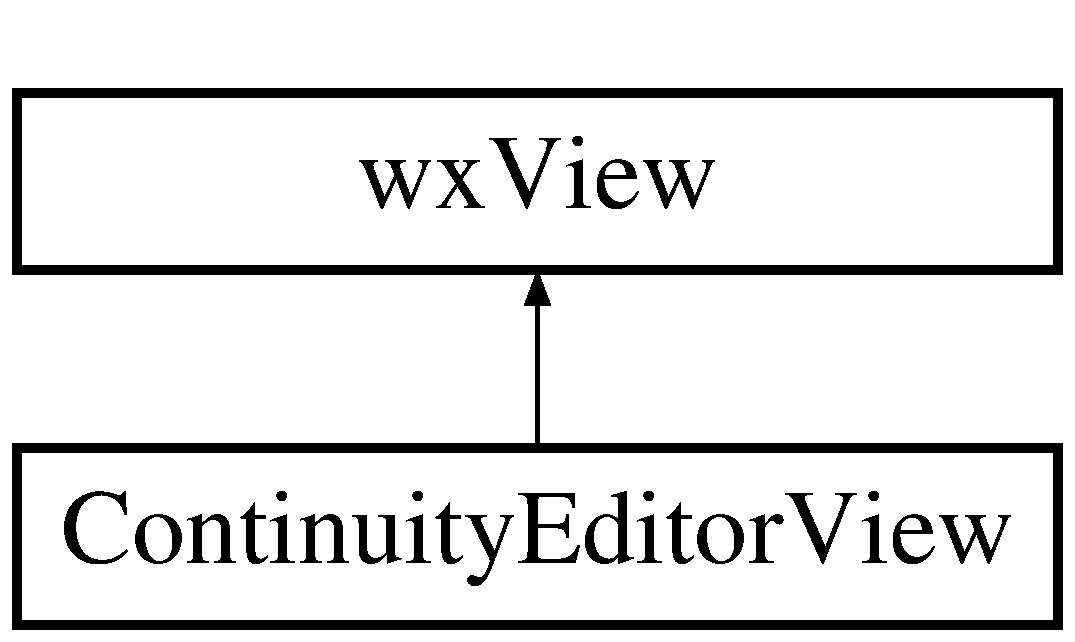
\includegraphics[height=2.000000cm]{a00060}
\end{center}
\end{figure}
\subsection*{Public Member Functions}
\begin{DoxyCompactItemize}
\item 
\hyperlink{a00060_a6c18f0bddca95ed60d18cea193d949d0}{Continuity\-Editor\-View} ()
\item 
\hyperlink{a00060_a18f4efb58a588aba9bafc57b376251ce}{$\sim$\-Continuity\-Editor\-View} ()
\item 
virtual void \hyperlink{a00060_addac4ca19641c7e984761b4f8028a8d9}{On\-Draw} (wx\-D\-C $\ast$dc)
\item 
virtual void \hyperlink{a00060_a82c91de0bdb32c27239170ad0c997cbd}{On\-Update} (wx\-View $\ast$sender, wx\-Object $\ast$hint=(wx\-Object $\ast$) N\-U\-L\-L)
\item 
void \hyperlink{a00060_a51db98325d30c848e1a3ec321ff2a578}{Do\-Set\-Continuity\-Text} (\hyperlink{a00216_a68cd84e0300be6f9ff4474682762c9ee}{S\-Y\-M\-B\-O\-L\-\_\-\-T\-Y\-P\-E} which, const wx\-String \&text)
\end{DoxyCompactItemize}


\subsection{Constructor \& Destructor Documentation}
\hypertarget{a00060_a6c18f0bddca95ed60d18cea193d949d0}{\index{Continuity\-Editor\-View@{Continuity\-Editor\-View}!Continuity\-Editor\-View@{Continuity\-Editor\-View}}
\index{Continuity\-Editor\-View@{Continuity\-Editor\-View}!ContinuityEditorView@{Continuity\-Editor\-View}}
\subsubsection[{Continuity\-Editor\-View}]{\setlength{\rightskip}{0pt plus 5cm}Continuity\-Editor\-View\-::\-Continuity\-Editor\-View (
\begin{DoxyParamCaption}
{}
\end{DoxyParamCaption}
)}}\label{a00060_a6c18f0bddca95ed60d18cea193d949d0}
\hypertarget{a00060_a18f4efb58a588aba9bafc57b376251ce}{\index{Continuity\-Editor\-View@{Continuity\-Editor\-View}!$\sim$\-Continuity\-Editor\-View@{$\sim$\-Continuity\-Editor\-View}}
\index{$\sim$\-Continuity\-Editor\-View@{$\sim$\-Continuity\-Editor\-View}!ContinuityEditorView@{Continuity\-Editor\-View}}
\subsubsection[{$\sim$\-Continuity\-Editor\-View}]{\setlength{\rightskip}{0pt plus 5cm}Continuity\-Editor\-View\-::$\sim$\-Continuity\-Editor\-View (
\begin{DoxyParamCaption}
{}
\end{DoxyParamCaption}
)}}\label{a00060_a18f4efb58a588aba9bafc57b376251ce}


\subsection{Member Function Documentation}
\hypertarget{a00060_a51db98325d30c848e1a3ec321ff2a578}{\index{Continuity\-Editor\-View@{Continuity\-Editor\-View}!Do\-Set\-Continuity\-Text@{Do\-Set\-Continuity\-Text}}
\index{Do\-Set\-Continuity\-Text@{Do\-Set\-Continuity\-Text}!ContinuityEditorView@{Continuity\-Editor\-View}}
\subsubsection[{Do\-Set\-Continuity\-Text}]{\setlength{\rightskip}{0pt plus 5cm}void Continuity\-Editor\-View\-::\-Do\-Set\-Continuity\-Text (
\begin{DoxyParamCaption}
\item[{{\bf S\-Y\-M\-B\-O\-L\-\_\-\-T\-Y\-P\-E}}]{which, }
\item[{const wx\-String \&}]{text}
\end{DoxyParamCaption}
)}}\label{a00060_a51db98325d30c848e1a3ec321ff2a578}
\hypertarget{a00060_addac4ca19641c7e984761b4f8028a8d9}{\index{Continuity\-Editor\-View@{Continuity\-Editor\-View}!On\-Draw@{On\-Draw}}
\index{On\-Draw@{On\-Draw}!ContinuityEditorView@{Continuity\-Editor\-View}}
\subsubsection[{On\-Draw}]{\setlength{\rightskip}{0pt plus 5cm}void Continuity\-Editor\-View\-::\-On\-Draw (
\begin{DoxyParamCaption}
\item[{wx\-D\-C $\ast$}]{dc}
\end{DoxyParamCaption}
)\hspace{0.3cm}{\ttfamily [virtual]}}}\label{a00060_addac4ca19641c7e984761b4f8028a8d9}
\hypertarget{a00060_a82c91de0bdb32c27239170ad0c997cbd}{\index{Continuity\-Editor\-View@{Continuity\-Editor\-View}!On\-Update@{On\-Update}}
\index{On\-Update@{On\-Update}!ContinuityEditorView@{Continuity\-Editor\-View}}
\subsubsection[{On\-Update}]{\setlength{\rightskip}{0pt plus 5cm}void Continuity\-Editor\-View\-::\-On\-Update (
\begin{DoxyParamCaption}
\item[{wx\-View $\ast$}]{sender, }
\item[{wx\-Object $\ast$}]{hint = {\ttfamily (wxObject~$\ast$)~NULL}}
\end{DoxyParamCaption}
)\hspace{0.3cm}{\ttfamily [virtual]}}}\label{a00060_a82c91de0bdb32c27239170ad0c997cbd}


The documentation for this class was generated from the following files\-:\begin{DoxyCompactItemize}
\item 
src/\hyperlink{a00193}{cont\-\_\-ui.\-h}\item 
src/\hyperlink{a00192}{cont\-\_\-ui.\-cpp}\end{DoxyCompactItemize}

\hypertarget{a00061}{\section{Cont\-Next\-Point Class Reference}
\label{a00061}\index{Cont\-Next\-Point@{Cont\-Next\-Point}}
}


{\ttfamily \#include $<$cont.\-h$>$}

Inheritance diagram for Cont\-Next\-Point\-:\begin{figure}[H]
\begin{center}
\leavevmode
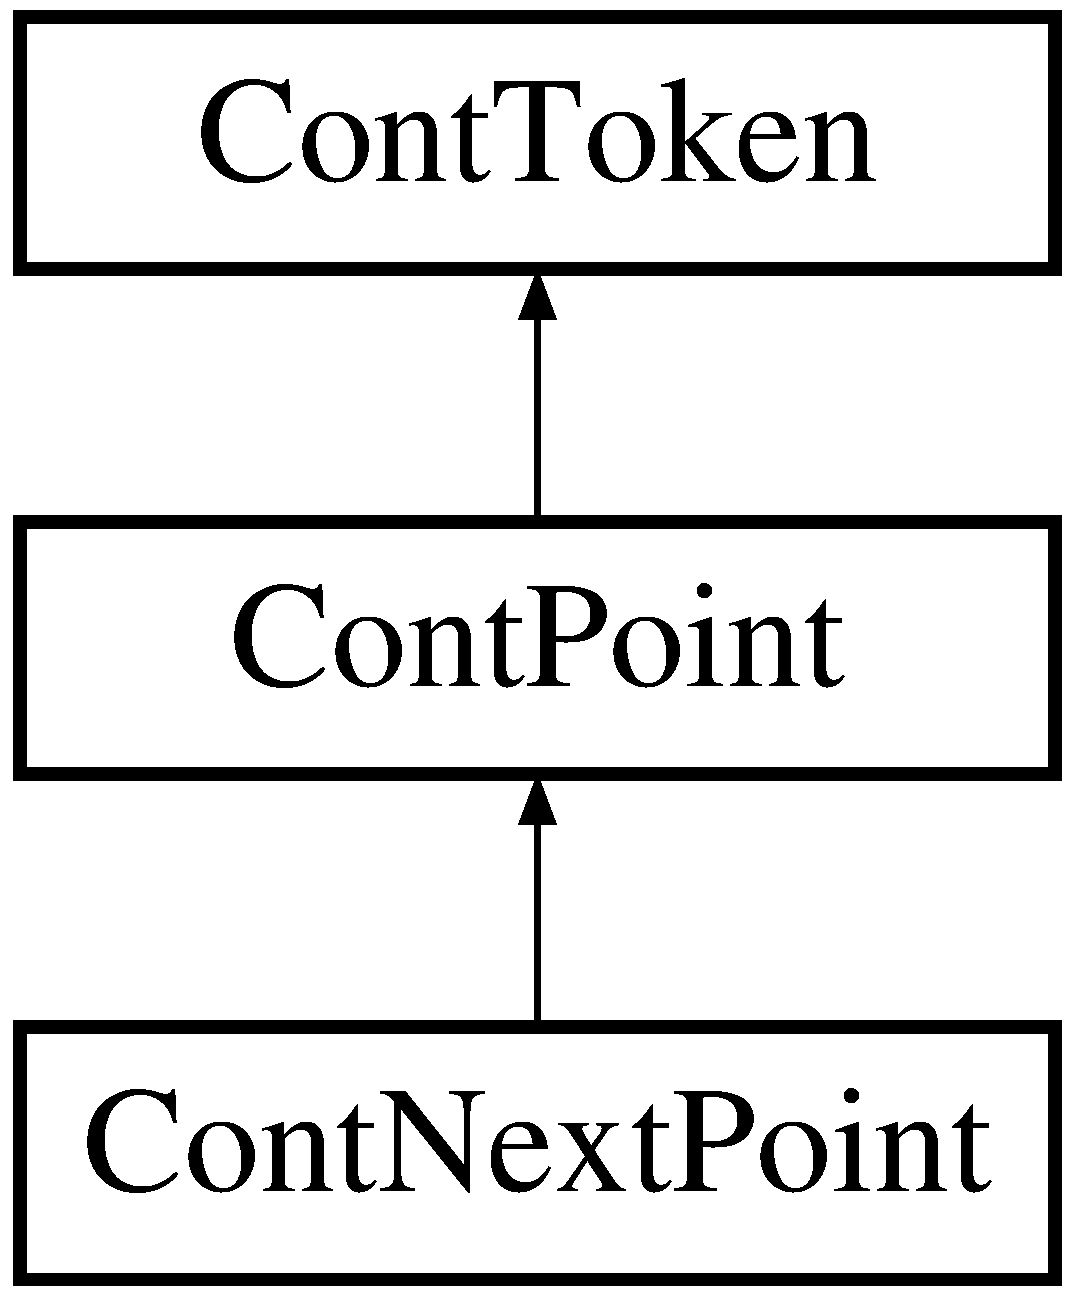
\includegraphics[height=3.000000cm]{a00061}
\end{center}
\end{figure}
\subsection*{Public Member Functions}
\begin{DoxyCompactItemize}
\item 
\hyperlink{a00061_a70e8f26d56c178f85c13bff61b0381eb}{Cont\-Next\-Point} ()
\item 
virtual \hyperlink{a00029}{C\-C\-\_\-coord} \hyperlink{a00061_a23ff9faf8489c21a3a105bc36aea068a}{Get} (\hyperlink{a00007}{Animate\-Compile} $\ast$anim) const 
\end{DoxyCompactItemize}
\subsection*{Additional Inherited Members}


\subsection{Constructor \& Destructor Documentation}
\hypertarget{a00061_a70e8f26d56c178f85c13bff61b0381eb}{\index{Cont\-Next\-Point@{Cont\-Next\-Point}!Cont\-Next\-Point@{Cont\-Next\-Point}}
\index{Cont\-Next\-Point@{Cont\-Next\-Point}!ContNextPoint@{Cont\-Next\-Point}}
\subsubsection[{Cont\-Next\-Point}]{\setlength{\rightskip}{0pt plus 5cm}Cont\-Next\-Point\-::\-Cont\-Next\-Point (
\begin{DoxyParamCaption}
{}
\end{DoxyParamCaption}
)\hspace{0.3cm}{\ttfamily [inline]}}}\label{a00061_a70e8f26d56c178f85c13bff61b0381eb}


\subsection{Member Function Documentation}
\hypertarget{a00061_a23ff9faf8489c21a3a105bc36aea068a}{\index{Cont\-Next\-Point@{Cont\-Next\-Point}!Get@{Get}}
\index{Get@{Get}!ContNextPoint@{Cont\-Next\-Point}}
\subsubsection[{Get}]{\setlength{\rightskip}{0pt plus 5cm}{\bf C\-C\-\_\-coord} Cont\-Next\-Point\-::\-Get (
\begin{DoxyParamCaption}
\item[{{\bf Animate\-Compile} $\ast$}]{anim}
\end{DoxyParamCaption}
) const\hspace{0.3cm}{\ttfamily [virtual]}}}\label{a00061_a23ff9faf8489c21a3a105bc36aea068a}


Reimplemented from \hyperlink{a00062_a1a51c628c19099b02f875c9bfb373a81}{Cont\-Point}.



The documentation for this class was generated from the following files\-:\begin{DoxyCompactItemize}
\item 
src/core/\hyperlink{a00218}{cont.\-h}\item 
src/core/\hyperlink{a00217}{cont.\-cpp}\end{DoxyCompactItemize}

\hypertarget{a00062}{\section{Cont\-Point Class Reference}
\label{a00062}\index{Cont\-Point@{Cont\-Point}}
}


{\ttfamily \#include $<$cont.\-h$>$}

Inheritance diagram for Cont\-Point\-:\begin{figure}[H]
\begin{center}
\leavevmode
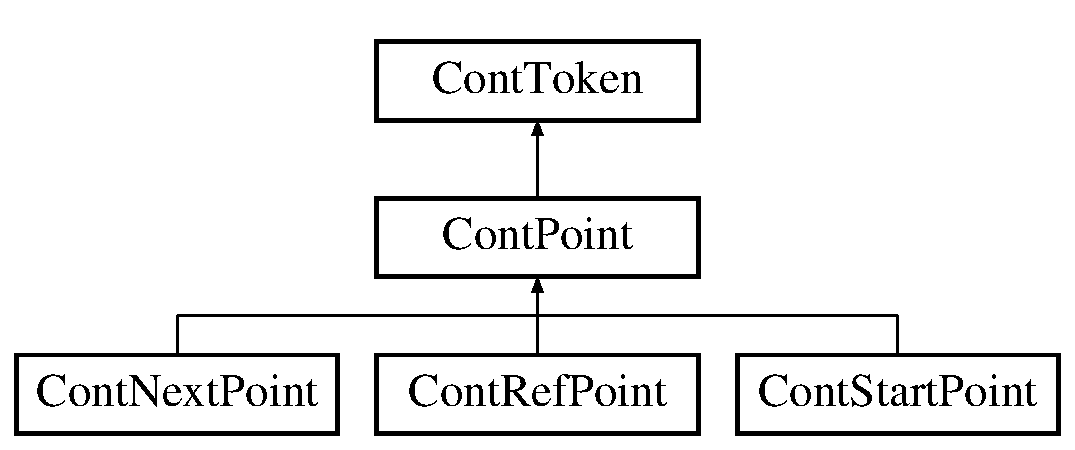
\includegraphics[height=3.000000cm]{a00062}
\end{center}
\end{figure}
\subsection*{Public Member Functions}
\begin{DoxyCompactItemize}
\item 
\hyperlink{a00062_a29f0b6e1212175fd0e963eaa3dae7aa4}{Cont\-Point} ()
\item 
virtual \hyperlink{a00062_af3235650468553a0bc1d06c666fb4c33}{$\sim$\-Cont\-Point} ()
\item 
virtual \hyperlink{a00029}{C\-C\-\_\-coord} \hyperlink{a00062_a1a51c628c19099b02f875c9bfb373a81}{Get} (\hyperlink{a00007}{Animate\-Compile} $\ast$anim) const 
\end{DoxyCompactItemize}
\subsection*{Additional Inherited Members}


\subsection{Constructor \& Destructor Documentation}
\hypertarget{a00062_a29f0b6e1212175fd0e963eaa3dae7aa4}{\index{Cont\-Point@{Cont\-Point}!Cont\-Point@{Cont\-Point}}
\index{Cont\-Point@{Cont\-Point}!ContPoint@{Cont\-Point}}
\subsubsection[{Cont\-Point}]{\setlength{\rightskip}{0pt plus 5cm}Cont\-Point\-::\-Cont\-Point (
\begin{DoxyParamCaption}
{}
\end{DoxyParamCaption}
)\hspace{0.3cm}{\ttfamily [inline]}}}\label{a00062_a29f0b6e1212175fd0e963eaa3dae7aa4}
\hypertarget{a00062_af3235650468553a0bc1d06c666fb4c33}{\index{Cont\-Point@{Cont\-Point}!$\sim$\-Cont\-Point@{$\sim$\-Cont\-Point}}
\index{$\sim$\-Cont\-Point@{$\sim$\-Cont\-Point}!ContPoint@{Cont\-Point}}
\subsubsection[{$\sim$\-Cont\-Point}]{\setlength{\rightskip}{0pt plus 5cm}Cont\-Point\-::$\sim$\-Cont\-Point (
\begin{DoxyParamCaption}
{}
\end{DoxyParamCaption}
)\hspace{0.3cm}{\ttfamily [virtual]}}}\label{a00062_af3235650468553a0bc1d06c666fb4c33}


\subsection{Member Function Documentation}
\hypertarget{a00062_a1a51c628c19099b02f875c9bfb373a81}{\index{Cont\-Point@{Cont\-Point}!Get@{Get}}
\index{Get@{Get}!ContPoint@{Cont\-Point}}
\subsubsection[{Get}]{\setlength{\rightskip}{0pt plus 5cm}{\bf C\-C\-\_\-coord} Cont\-Point\-::\-Get (
\begin{DoxyParamCaption}
\item[{{\bf Animate\-Compile} $\ast$}]{anim}
\end{DoxyParamCaption}
) const\hspace{0.3cm}{\ttfamily [virtual]}}}\label{a00062_a1a51c628c19099b02f875c9bfb373a81}


Reimplemented in \hyperlink{a00083_a858ab0673dca663beca109f8a9c8f5f3}{Cont\-Ref\-Point}, \hyperlink{a00061_a23ff9faf8489c21a3a105bc36aea068a}{Cont\-Next\-Point}, and \hyperlink{a00084_ada0ed3543db7b7888dec8113a5fab3d6}{Cont\-Start\-Point}.



The documentation for this class was generated from the following files\-:\begin{DoxyCompactItemize}
\item 
src/core/\hyperlink{a00218}{cont.\-h}\item 
src/core/\hyperlink{a00217}{cont.\-cpp}\end{DoxyCompactItemize}

\hypertarget{a00063}{\section{Cont\-Proc\-Blam Class Reference}
\label{a00063}\index{Cont\-Proc\-Blam@{Cont\-Proc\-Blam}}
}


{\ttfamily \#include $<$cont.\-h$>$}

Inheritance diagram for Cont\-Proc\-Blam\-:\begin{figure}[H]
\begin{center}
\leavevmode
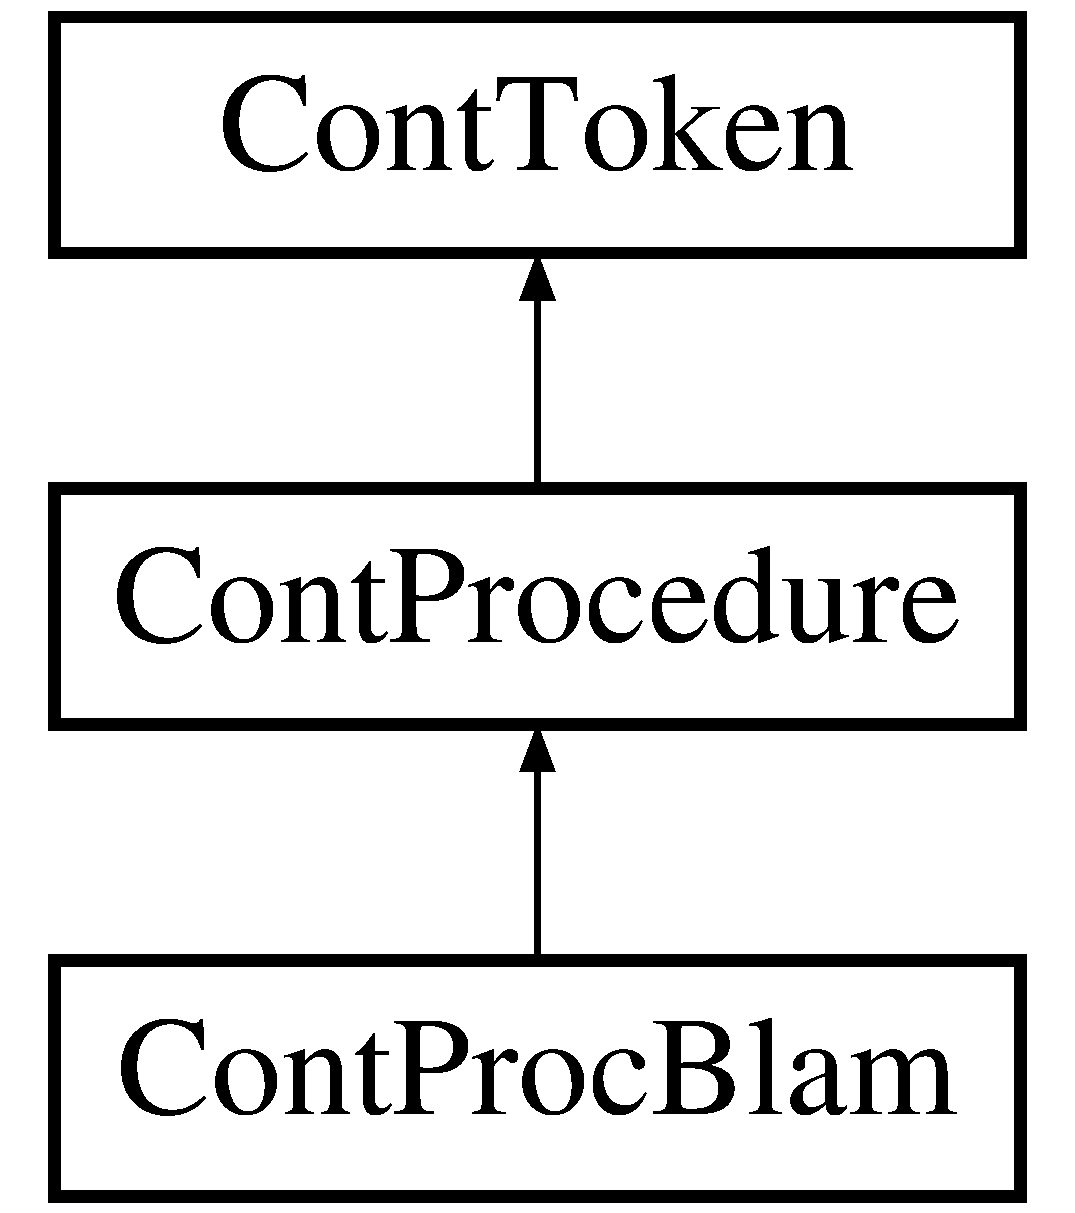
\includegraphics[height=3.000000cm]{a00063}
\end{center}
\end{figure}
\subsection*{Public Member Functions}
\begin{DoxyCompactItemize}
\item 
virtual void \hyperlink{a00063_a049c64760a90035f4a4fadb1c190499e}{Compile} (\hyperlink{a00007}{Animate\-Compile} $\ast$anim)
\end{DoxyCompactItemize}
\subsection*{Additional Inherited Members}


\subsection{Member Function Documentation}
\hypertarget{a00063_a049c64760a90035f4a4fadb1c190499e}{\index{Cont\-Proc\-Blam@{Cont\-Proc\-Blam}!Compile@{Compile}}
\index{Compile@{Compile}!ContProcBlam@{Cont\-Proc\-Blam}}
\subsubsection[{Compile}]{\setlength{\rightskip}{0pt plus 5cm}void Cont\-Proc\-Blam\-::\-Compile (
\begin{DoxyParamCaption}
\item[{{\bf Animate\-Compile} $\ast$}]{anim}
\end{DoxyParamCaption}
)\hspace{0.3cm}{\ttfamily [virtual]}}}\label{a00063_a049c64760a90035f4a4fadb1c190499e}


Implements \hyperlink{a00067_a7f7adefe250a00b3778669ef649f03ac}{Cont\-Procedure}.



The documentation for this class was generated from the following files\-:\begin{DoxyCompactItemize}
\item 
src/core/\hyperlink{a00218}{cont.\-h}\item 
src/core/\hyperlink{a00217}{cont.\-cpp}\end{DoxyCompactItemize}

\hypertarget{a00064}{\section{Cont\-Proc\-C\-M Class Reference}
\label{a00064}\index{Cont\-Proc\-C\-M@{Cont\-Proc\-C\-M}}
}


{\ttfamily \#include $<$cont.\-h$>$}

Inheritance diagram for Cont\-Proc\-C\-M\-:\begin{figure}[H]
\begin{center}
\leavevmode
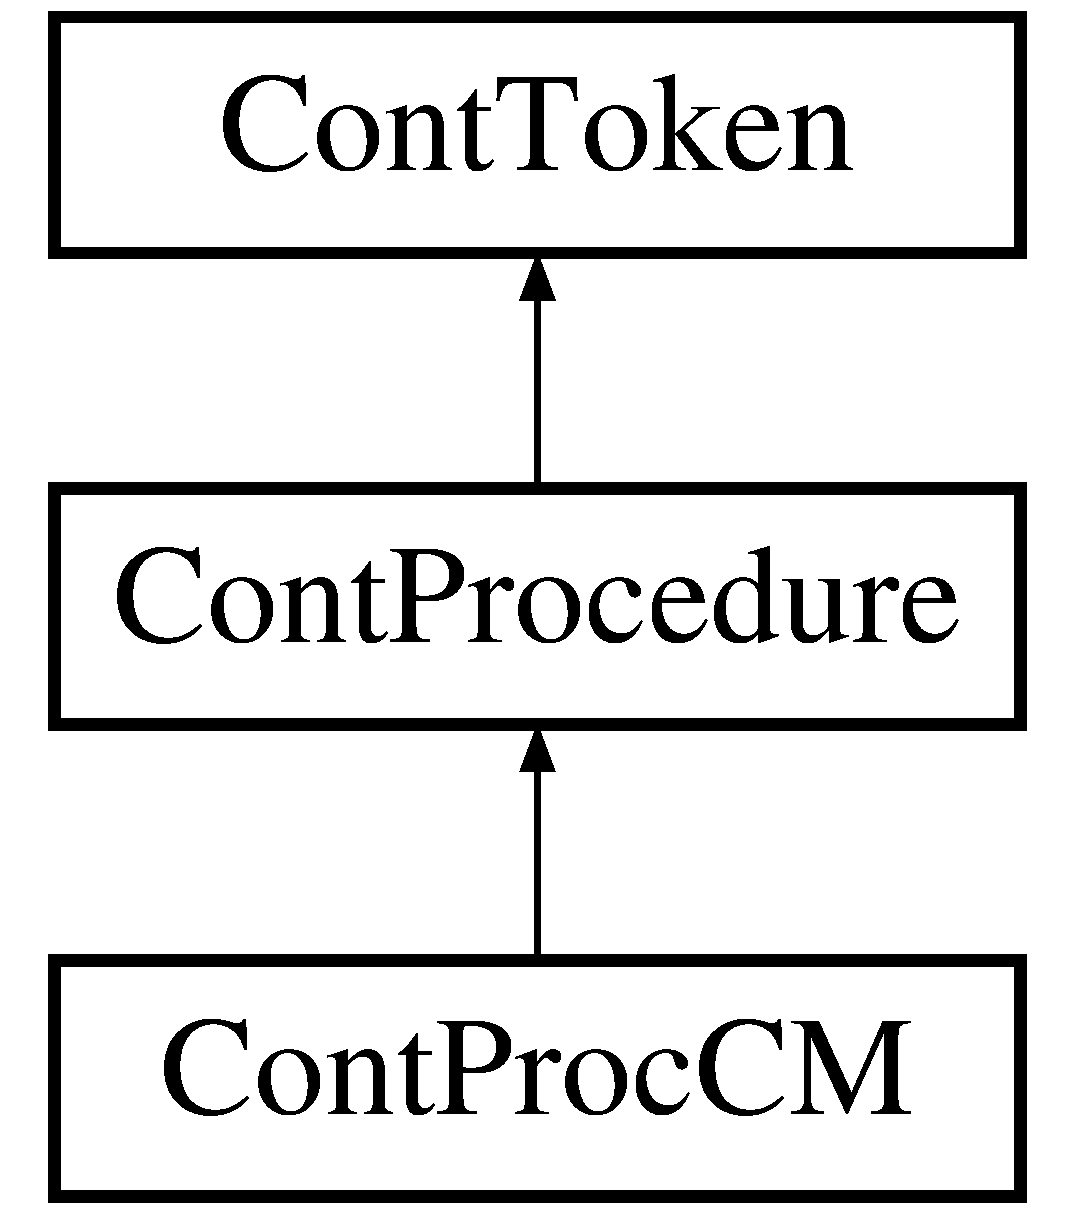
\includegraphics[height=3.000000cm]{a00064}
\end{center}
\end{figure}
\subsection*{Public Member Functions}
\begin{DoxyCompactItemize}
\item 
\hyperlink{a00064_ac6b4592fce2ad41d07d94aa8e14a22ba}{Cont\-Proc\-C\-M} (\hyperlink{a00062}{Cont\-Point} $\ast$p1, \hyperlink{a00062}{Cont\-Point} $\ast$p2, \hyperlink{a00086}{Cont\-Value} $\ast$steps, \hyperlink{a00086}{Cont\-Value} $\ast$d1, \hyperlink{a00086}{Cont\-Value} $\ast$d2, \hyperlink{a00086}{Cont\-Value} $\ast$beats)
\item 
virtual \hyperlink{a00064_a5cfc324ae4649adab5e256a5e0ea8096}{$\sim$\-Cont\-Proc\-C\-M} ()
\item 
virtual void \hyperlink{a00064_ae3d0ef74c8e17080072c537f29c17519}{Compile} (\hyperlink{a00007}{Animate\-Compile} $\ast$anim)
\end{DoxyCompactItemize}
\subsection*{Private Attributes}
\begin{DoxyCompactItemize}
\item 
\hyperlink{a00062}{Cont\-Point} $\ast$ \hyperlink{a00064_ab26de80a5d39bbc258c2f1a0c891e019}{pnt1}
\item 
\hyperlink{a00062}{Cont\-Point} $\ast$ \hyperlink{a00064_aac5833fb80c9a5413aca7cbbda125a2c}{pnt2}
\item 
\hyperlink{a00086}{Cont\-Value} $\ast$ \hyperlink{a00064_a5c5d9e8f0709600e603d41d1840bb134}{stps}
\item 
\hyperlink{a00086}{Cont\-Value} $\ast$ \hyperlink{a00064_abbb93432c6a51264b680e9971dfe2d21}{dir1}
\item 
\hyperlink{a00086}{Cont\-Value} $\ast$ \hyperlink{a00064_a9ca842f12168d7910db6f009005640e6}{dir2}
\item 
\hyperlink{a00086}{Cont\-Value} $\ast$ \hyperlink{a00064_a196f9549aa5ec6e90fd0abe2940196a1}{numbeats}
\end{DoxyCompactItemize}
\subsection*{Additional Inherited Members}


\subsection{Constructor \& Destructor Documentation}
\hypertarget{a00064_ac6b4592fce2ad41d07d94aa8e14a22ba}{\index{Cont\-Proc\-C\-M@{Cont\-Proc\-C\-M}!Cont\-Proc\-C\-M@{Cont\-Proc\-C\-M}}
\index{Cont\-Proc\-C\-M@{Cont\-Proc\-C\-M}!ContProcCM@{Cont\-Proc\-C\-M}}
\subsubsection[{Cont\-Proc\-C\-M}]{\setlength{\rightskip}{0pt plus 5cm}Cont\-Proc\-C\-M\-::\-Cont\-Proc\-C\-M (
\begin{DoxyParamCaption}
\item[{{\bf Cont\-Point} $\ast$}]{p1, }
\item[{{\bf Cont\-Point} $\ast$}]{p2, }
\item[{{\bf Cont\-Value} $\ast$}]{steps, }
\item[{{\bf Cont\-Value} $\ast$}]{d1, }
\item[{{\bf Cont\-Value} $\ast$}]{d2, }
\item[{{\bf Cont\-Value} $\ast$}]{beats}
\end{DoxyParamCaption}
)\hspace{0.3cm}{\ttfamily [inline]}}}\label{a00064_ac6b4592fce2ad41d07d94aa8e14a22ba}
\hypertarget{a00064_a5cfc324ae4649adab5e256a5e0ea8096}{\index{Cont\-Proc\-C\-M@{Cont\-Proc\-C\-M}!$\sim$\-Cont\-Proc\-C\-M@{$\sim$\-Cont\-Proc\-C\-M}}
\index{$\sim$\-Cont\-Proc\-C\-M@{$\sim$\-Cont\-Proc\-C\-M}!ContProcCM@{Cont\-Proc\-C\-M}}
\subsubsection[{$\sim$\-Cont\-Proc\-C\-M}]{\setlength{\rightskip}{0pt plus 5cm}Cont\-Proc\-C\-M\-::$\sim$\-Cont\-Proc\-C\-M (
\begin{DoxyParamCaption}
{}
\end{DoxyParamCaption}
)\hspace{0.3cm}{\ttfamily [virtual]}}}\label{a00064_a5cfc324ae4649adab5e256a5e0ea8096}


\subsection{Member Function Documentation}
\hypertarget{a00064_ae3d0ef74c8e17080072c537f29c17519}{\index{Cont\-Proc\-C\-M@{Cont\-Proc\-C\-M}!Compile@{Compile}}
\index{Compile@{Compile}!ContProcCM@{Cont\-Proc\-C\-M}}
\subsubsection[{Compile}]{\setlength{\rightskip}{0pt plus 5cm}void Cont\-Proc\-C\-M\-::\-Compile (
\begin{DoxyParamCaption}
\item[{{\bf Animate\-Compile} $\ast$}]{anim}
\end{DoxyParamCaption}
)\hspace{0.3cm}{\ttfamily [virtual]}}}\label{a00064_ae3d0ef74c8e17080072c537f29c17519}


Implements \hyperlink{a00067_a7f7adefe250a00b3778669ef649f03ac}{Cont\-Procedure}.



\subsection{Member Data Documentation}
\hypertarget{a00064_abbb93432c6a51264b680e9971dfe2d21}{\index{Cont\-Proc\-C\-M@{Cont\-Proc\-C\-M}!dir1@{dir1}}
\index{dir1@{dir1}!ContProcCM@{Cont\-Proc\-C\-M}}
\subsubsection[{dir1}]{\setlength{\rightskip}{0pt plus 5cm}{\bf Cont\-Value} $\ast$ Cont\-Proc\-C\-M\-::dir1\hspace{0.3cm}{\ttfamily [private]}}}\label{a00064_abbb93432c6a51264b680e9971dfe2d21}
\hypertarget{a00064_a9ca842f12168d7910db6f009005640e6}{\index{Cont\-Proc\-C\-M@{Cont\-Proc\-C\-M}!dir2@{dir2}}
\index{dir2@{dir2}!ContProcCM@{Cont\-Proc\-C\-M}}
\subsubsection[{dir2}]{\setlength{\rightskip}{0pt plus 5cm}{\bf Cont\-Value} $\ast$ Cont\-Proc\-C\-M\-::dir2\hspace{0.3cm}{\ttfamily [private]}}}\label{a00064_a9ca842f12168d7910db6f009005640e6}
\hypertarget{a00064_a196f9549aa5ec6e90fd0abe2940196a1}{\index{Cont\-Proc\-C\-M@{Cont\-Proc\-C\-M}!numbeats@{numbeats}}
\index{numbeats@{numbeats}!ContProcCM@{Cont\-Proc\-C\-M}}
\subsubsection[{numbeats}]{\setlength{\rightskip}{0pt plus 5cm}{\bf Cont\-Value} $\ast$ Cont\-Proc\-C\-M\-::numbeats\hspace{0.3cm}{\ttfamily [private]}}}\label{a00064_a196f9549aa5ec6e90fd0abe2940196a1}
\hypertarget{a00064_ab26de80a5d39bbc258c2f1a0c891e019}{\index{Cont\-Proc\-C\-M@{Cont\-Proc\-C\-M}!pnt1@{pnt1}}
\index{pnt1@{pnt1}!ContProcCM@{Cont\-Proc\-C\-M}}
\subsubsection[{pnt1}]{\setlength{\rightskip}{0pt plus 5cm}{\bf Cont\-Point}$\ast$ Cont\-Proc\-C\-M\-::pnt1\hspace{0.3cm}{\ttfamily [private]}}}\label{a00064_ab26de80a5d39bbc258c2f1a0c891e019}
\hypertarget{a00064_aac5833fb80c9a5413aca7cbbda125a2c}{\index{Cont\-Proc\-C\-M@{Cont\-Proc\-C\-M}!pnt2@{pnt2}}
\index{pnt2@{pnt2}!ContProcCM@{Cont\-Proc\-C\-M}}
\subsubsection[{pnt2}]{\setlength{\rightskip}{0pt plus 5cm}{\bf Cont\-Point} $\ast$ Cont\-Proc\-C\-M\-::pnt2\hspace{0.3cm}{\ttfamily [private]}}}\label{a00064_aac5833fb80c9a5413aca7cbbda125a2c}
\hypertarget{a00064_a5c5d9e8f0709600e603d41d1840bb134}{\index{Cont\-Proc\-C\-M@{Cont\-Proc\-C\-M}!stps@{stps}}
\index{stps@{stps}!ContProcCM@{Cont\-Proc\-C\-M}}
\subsubsection[{stps}]{\setlength{\rightskip}{0pt plus 5cm}{\bf Cont\-Value}$\ast$ Cont\-Proc\-C\-M\-::stps\hspace{0.3cm}{\ttfamily [private]}}}\label{a00064_a5c5d9e8f0709600e603d41d1840bb134}


The documentation for this class was generated from the following files\-:\begin{DoxyCompactItemize}
\item 
src/core/\hyperlink{a00218}{cont.\-h}\item 
src/core/\hyperlink{a00217}{cont.\-cpp}\end{DoxyCompactItemize}

\hypertarget{a00065}{\section{Cont\-Proc\-D\-M\-C\-M Class Reference}
\label{a00065}\index{Cont\-Proc\-D\-M\-C\-M@{Cont\-Proc\-D\-M\-C\-M}}
}


{\ttfamily \#include $<$cont.\-h$>$}

Inheritance diagram for Cont\-Proc\-D\-M\-C\-M\-:\begin{figure}[H]
\begin{center}
\leavevmode
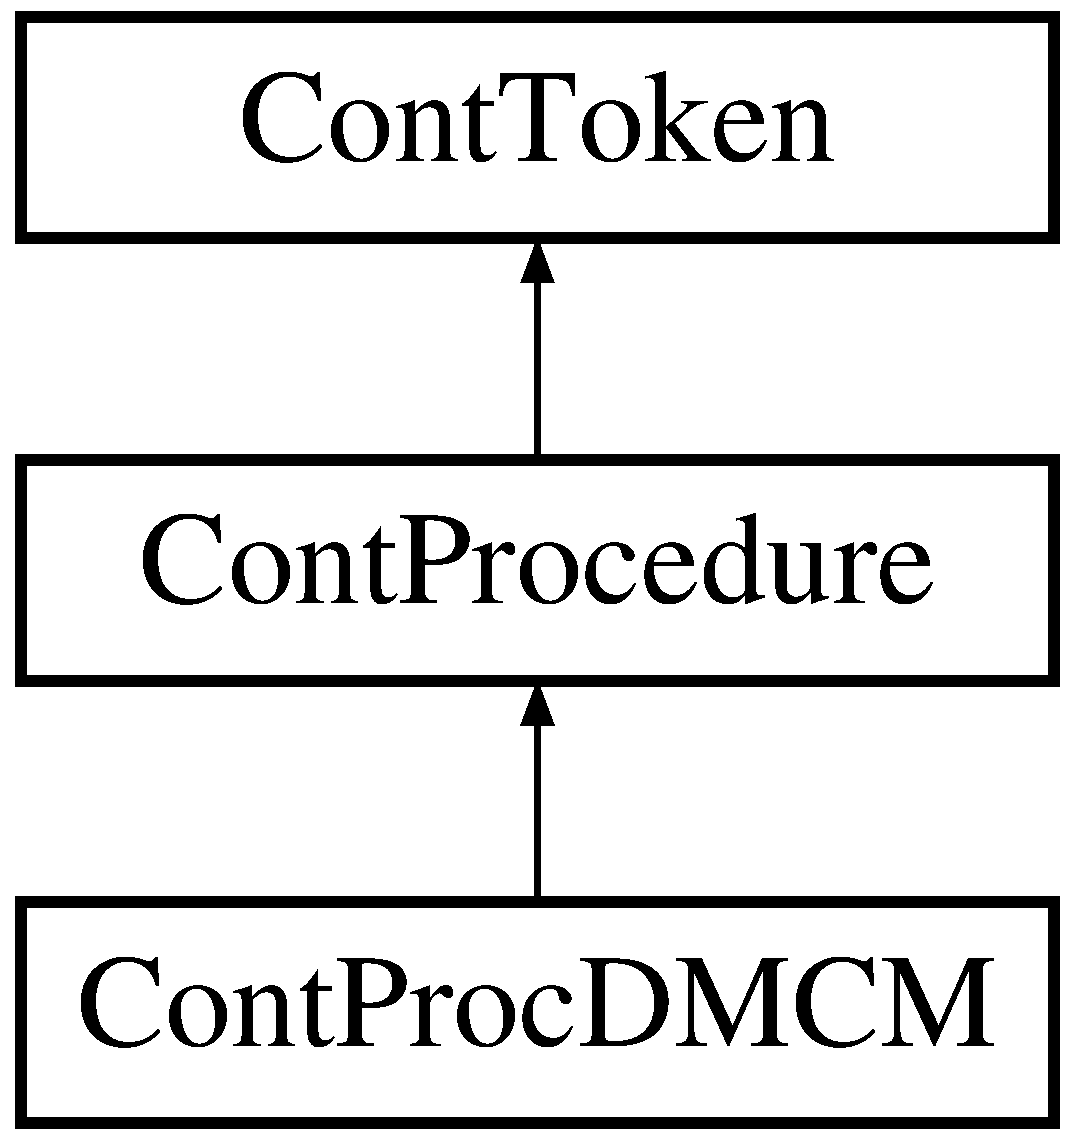
\includegraphics[height=3.000000cm]{a00065}
\end{center}
\end{figure}
\subsection*{Public Member Functions}
\begin{DoxyCompactItemize}
\item 
\hyperlink{a00065_acbc50672578ded6f655eb50a02208776}{Cont\-Proc\-D\-M\-C\-M} (\hyperlink{a00062}{Cont\-Point} $\ast$p1, \hyperlink{a00062}{Cont\-Point} $\ast$p2, \hyperlink{a00086}{Cont\-Value} $\ast$beats)
\item 
virtual \hyperlink{a00065_a6bfe1651fbaa9f23a5fd3f5330c2d364}{$\sim$\-Cont\-Proc\-D\-M\-C\-M} ()
\item 
virtual void \hyperlink{a00065_a90453323245d51cccd91dd50802e9f66}{Compile} (\hyperlink{a00007}{Animate\-Compile} $\ast$anim)
\end{DoxyCompactItemize}
\subsection*{Private Attributes}
\begin{DoxyCompactItemize}
\item 
\hyperlink{a00062}{Cont\-Point} $\ast$ \hyperlink{a00065_a52e7aee506251aa08d2c1460e56d0046}{pnt1}
\item 
\hyperlink{a00062}{Cont\-Point} $\ast$ \hyperlink{a00065_a6c0c5b4a783714400be626e0989a7ed9}{pnt2}
\item 
\hyperlink{a00086}{Cont\-Value} $\ast$ \hyperlink{a00065_aee975972e470093cdd88861077d4774a}{numbeats}
\end{DoxyCompactItemize}
\subsection*{Additional Inherited Members}


\subsection{Constructor \& Destructor Documentation}
\hypertarget{a00065_acbc50672578ded6f655eb50a02208776}{\index{Cont\-Proc\-D\-M\-C\-M@{Cont\-Proc\-D\-M\-C\-M}!Cont\-Proc\-D\-M\-C\-M@{Cont\-Proc\-D\-M\-C\-M}}
\index{Cont\-Proc\-D\-M\-C\-M@{Cont\-Proc\-D\-M\-C\-M}!ContProcDMCM@{Cont\-Proc\-D\-M\-C\-M}}
\subsubsection[{Cont\-Proc\-D\-M\-C\-M}]{\setlength{\rightskip}{0pt plus 5cm}Cont\-Proc\-D\-M\-C\-M\-::\-Cont\-Proc\-D\-M\-C\-M (
\begin{DoxyParamCaption}
\item[{{\bf Cont\-Point} $\ast$}]{p1, }
\item[{{\bf Cont\-Point} $\ast$}]{p2, }
\item[{{\bf Cont\-Value} $\ast$}]{beats}
\end{DoxyParamCaption}
)\hspace{0.3cm}{\ttfamily [inline]}}}\label{a00065_acbc50672578ded6f655eb50a02208776}
\hypertarget{a00065_a6bfe1651fbaa9f23a5fd3f5330c2d364}{\index{Cont\-Proc\-D\-M\-C\-M@{Cont\-Proc\-D\-M\-C\-M}!$\sim$\-Cont\-Proc\-D\-M\-C\-M@{$\sim$\-Cont\-Proc\-D\-M\-C\-M}}
\index{$\sim$\-Cont\-Proc\-D\-M\-C\-M@{$\sim$\-Cont\-Proc\-D\-M\-C\-M}!ContProcDMCM@{Cont\-Proc\-D\-M\-C\-M}}
\subsubsection[{$\sim$\-Cont\-Proc\-D\-M\-C\-M}]{\setlength{\rightskip}{0pt plus 5cm}Cont\-Proc\-D\-M\-C\-M\-::$\sim$\-Cont\-Proc\-D\-M\-C\-M (
\begin{DoxyParamCaption}
{}
\end{DoxyParamCaption}
)\hspace{0.3cm}{\ttfamily [virtual]}}}\label{a00065_a6bfe1651fbaa9f23a5fd3f5330c2d364}


\subsection{Member Function Documentation}
\hypertarget{a00065_a90453323245d51cccd91dd50802e9f66}{\index{Cont\-Proc\-D\-M\-C\-M@{Cont\-Proc\-D\-M\-C\-M}!Compile@{Compile}}
\index{Compile@{Compile}!ContProcDMCM@{Cont\-Proc\-D\-M\-C\-M}}
\subsubsection[{Compile}]{\setlength{\rightskip}{0pt plus 5cm}void Cont\-Proc\-D\-M\-C\-M\-::\-Compile (
\begin{DoxyParamCaption}
\item[{{\bf Animate\-Compile} $\ast$}]{anim}
\end{DoxyParamCaption}
)\hspace{0.3cm}{\ttfamily [virtual]}}}\label{a00065_a90453323245d51cccd91dd50802e9f66}


Implements \hyperlink{a00067_a7f7adefe250a00b3778669ef649f03ac}{Cont\-Procedure}.



\subsection{Member Data Documentation}
\hypertarget{a00065_aee975972e470093cdd88861077d4774a}{\index{Cont\-Proc\-D\-M\-C\-M@{Cont\-Proc\-D\-M\-C\-M}!numbeats@{numbeats}}
\index{numbeats@{numbeats}!ContProcDMCM@{Cont\-Proc\-D\-M\-C\-M}}
\subsubsection[{numbeats}]{\setlength{\rightskip}{0pt plus 5cm}{\bf Cont\-Value}$\ast$ Cont\-Proc\-D\-M\-C\-M\-::numbeats\hspace{0.3cm}{\ttfamily [private]}}}\label{a00065_aee975972e470093cdd88861077d4774a}
\hypertarget{a00065_a52e7aee506251aa08d2c1460e56d0046}{\index{Cont\-Proc\-D\-M\-C\-M@{Cont\-Proc\-D\-M\-C\-M}!pnt1@{pnt1}}
\index{pnt1@{pnt1}!ContProcDMCM@{Cont\-Proc\-D\-M\-C\-M}}
\subsubsection[{pnt1}]{\setlength{\rightskip}{0pt plus 5cm}{\bf Cont\-Point}$\ast$ Cont\-Proc\-D\-M\-C\-M\-::pnt1\hspace{0.3cm}{\ttfamily [private]}}}\label{a00065_a52e7aee506251aa08d2c1460e56d0046}
\hypertarget{a00065_a6c0c5b4a783714400be626e0989a7ed9}{\index{Cont\-Proc\-D\-M\-C\-M@{Cont\-Proc\-D\-M\-C\-M}!pnt2@{pnt2}}
\index{pnt2@{pnt2}!ContProcDMCM@{Cont\-Proc\-D\-M\-C\-M}}
\subsubsection[{pnt2}]{\setlength{\rightskip}{0pt plus 5cm}{\bf Cont\-Point} $\ast$ Cont\-Proc\-D\-M\-C\-M\-::pnt2\hspace{0.3cm}{\ttfamily [private]}}}\label{a00065_a6c0c5b4a783714400be626e0989a7ed9}


The documentation for this class was generated from the following files\-:\begin{DoxyCompactItemize}
\item 
src/core/\hyperlink{a00218}{cont.\-h}\item 
src/core/\hyperlink{a00217}{cont.\-cpp}\end{DoxyCompactItemize}

\hypertarget{a00066}{\section{Cont\-Proc\-D\-M\-H\-S Class Reference}
\label{a00066}\index{Cont\-Proc\-D\-M\-H\-S@{Cont\-Proc\-D\-M\-H\-S}}
}


{\ttfamily \#include $<$cont.\-h$>$}

Inheritance diagram for Cont\-Proc\-D\-M\-H\-S\-:\begin{figure}[H]
\begin{center}
\leavevmode
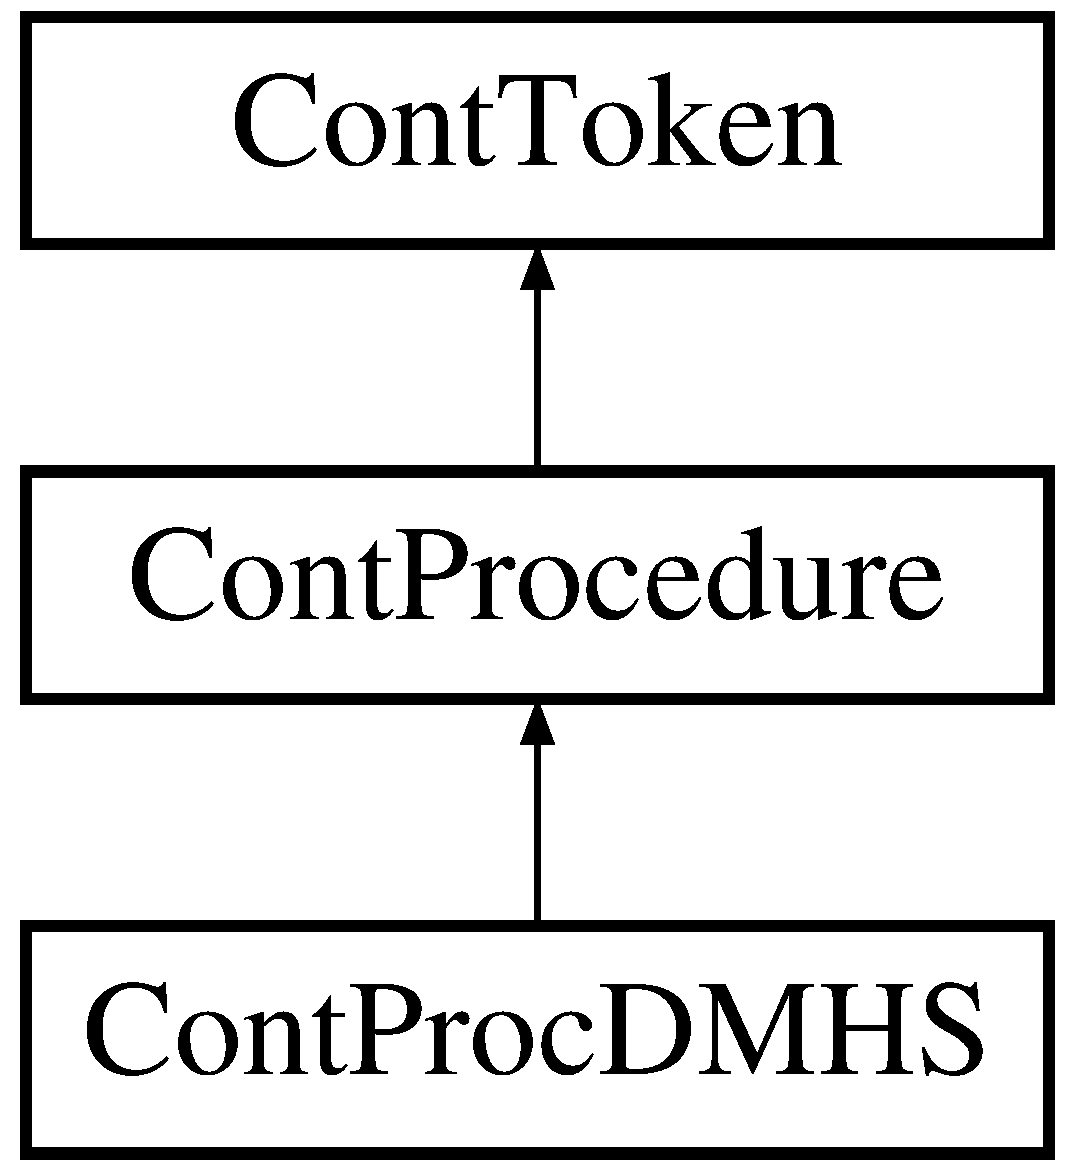
\includegraphics[height=3.000000cm]{a00066}
\end{center}
\end{figure}
\subsection*{Public Member Functions}
\begin{DoxyCompactItemize}
\item 
\hyperlink{a00066_a3cae677a99c24d80015bcda837e36b18}{Cont\-Proc\-D\-M\-H\-S} (\hyperlink{a00062}{Cont\-Point} $\ast$p)
\item 
virtual \hyperlink{a00066_a1b681a7c36ded763611634186943c1b4}{$\sim$\-Cont\-Proc\-D\-M\-H\-S} ()
\item 
virtual void \hyperlink{a00066_aa12b04f473128f3d07139649ef944317}{Compile} (\hyperlink{a00007}{Animate\-Compile} $\ast$anim)
\end{DoxyCompactItemize}
\subsection*{Private Attributes}
\begin{DoxyCompactItemize}
\item 
\hyperlink{a00062}{Cont\-Point} $\ast$ \hyperlink{a00066_a517ed8f7ba18697cdf76b10c2b95c499}{pnt}
\end{DoxyCompactItemize}
\subsection*{Additional Inherited Members}


\subsection{Constructor \& Destructor Documentation}
\hypertarget{a00066_a3cae677a99c24d80015bcda837e36b18}{\index{Cont\-Proc\-D\-M\-H\-S@{Cont\-Proc\-D\-M\-H\-S}!Cont\-Proc\-D\-M\-H\-S@{Cont\-Proc\-D\-M\-H\-S}}
\index{Cont\-Proc\-D\-M\-H\-S@{Cont\-Proc\-D\-M\-H\-S}!ContProcDMHS@{Cont\-Proc\-D\-M\-H\-S}}
\subsubsection[{Cont\-Proc\-D\-M\-H\-S}]{\setlength{\rightskip}{0pt plus 5cm}Cont\-Proc\-D\-M\-H\-S\-::\-Cont\-Proc\-D\-M\-H\-S (
\begin{DoxyParamCaption}
\item[{{\bf Cont\-Point} $\ast$}]{p}
\end{DoxyParamCaption}
)\hspace{0.3cm}{\ttfamily [inline]}}}\label{a00066_a3cae677a99c24d80015bcda837e36b18}
\hypertarget{a00066_a1b681a7c36ded763611634186943c1b4}{\index{Cont\-Proc\-D\-M\-H\-S@{Cont\-Proc\-D\-M\-H\-S}!$\sim$\-Cont\-Proc\-D\-M\-H\-S@{$\sim$\-Cont\-Proc\-D\-M\-H\-S}}
\index{$\sim$\-Cont\-Proc\-D\-M\-H\-S@{$\sim$\-Cont\-Proc\-D\-M\-H\-S}!ContProcDMHS@{Cont\-Proc\-D\-M\-H\-S}}
\subsubsection[{$\sim$\-Cont\-Proc\-D\-M\-H\-S}]{\setlength{\rightskip}{0pt plus 5cm}Cont\-Proc\-D\-M\-H\-S\-::$\sim$\-Cont\-Proc\-D\-M\-H\-S (
\begin{DoxyParamCaption}
{}
\end{DoxyParamCaption}
)\hspace{0.3cm}{\ttfamily [virtual]}}}\label{a00066_a1b681a7c36ded763611634186943c1b4}


\subsection{Member Function Documentation}
\hypertarget{a00066_aa12b04f473128f3d07139649ef944317}{\index{Cont\-Proc\-D\-M\-H\-S@{Cont\-Proc\-D\-M\-H\-S}!Compile@{Compile}}
\index{Compile@{Compile}!ContProcDMHS@{Cont\-Proc\-D\-M\-H\-S}}
\subsubsection[{Compile}]{\setlength{\rightskip}{0pt plus 5cm}void Cont\-Proc\-D\-M\-H\-S\-::\-Compile (
\begin{DoxyParamCaption}
\item[{{\bf Animate\-Compile} $\ast$}]{anim}
\end{DoxyParamCaption}
)\hspace{0.3cm}{\ttfamily [virtual]}}}\label{a00066_aa12b04f473128f3d07139649ef944317}


Implements \hyperlink{a00067_a7f7adefe250a00b3778669ef649f03ac}{Cont\-Procedure}.



\subsection{Member Data Documentation}
\hypertarget{a00066_a517ed8f7ba18697cdf76b10c2b95c499}{\index{Cont\-Proc\-D\-M\-H\-S@{Cont\-Proc\-D\-M\-H\-S}!pnt@{pnt}}
\index{pnt@{pnt}!ContProcDMHS@{Cont\-Proc\-D\-M\-H\-S}}
\subsubsection[{pnt}]{\setlength{\rightskip}{0pt plus 5cm}{\bf Cont\-Point}$\ast$ Cont\-Proc\-D\-M\-H\-S\-::pnt\hspace{0.3cm}{\ttfamily [private]}}}\label{a00066_a517ed8f7ba18697cdf76b10c2b95c499}


The documentation for this class was generated from the following files\-:\begin{DoxyCompactItemize}
\item 
src/core/\hyperlink{a00218}{cont.\-h}\item 
src/core/\hyperlink{a00217}{cont.\-cpp}\end{DoxyCompactItemize}

\hypertarget{a00067}{\section{Cont\-Procedure Class Reference}
\label{a00067}\index{Cont\-Procedure@{Cont\-Procedure}}
}


{\ttfamily \#include $<$cont.\-h$>$}

Inheritance diagram for Cont\-Procedure\-:\begin{figure}[H]
\begin{center}
\leavevmode
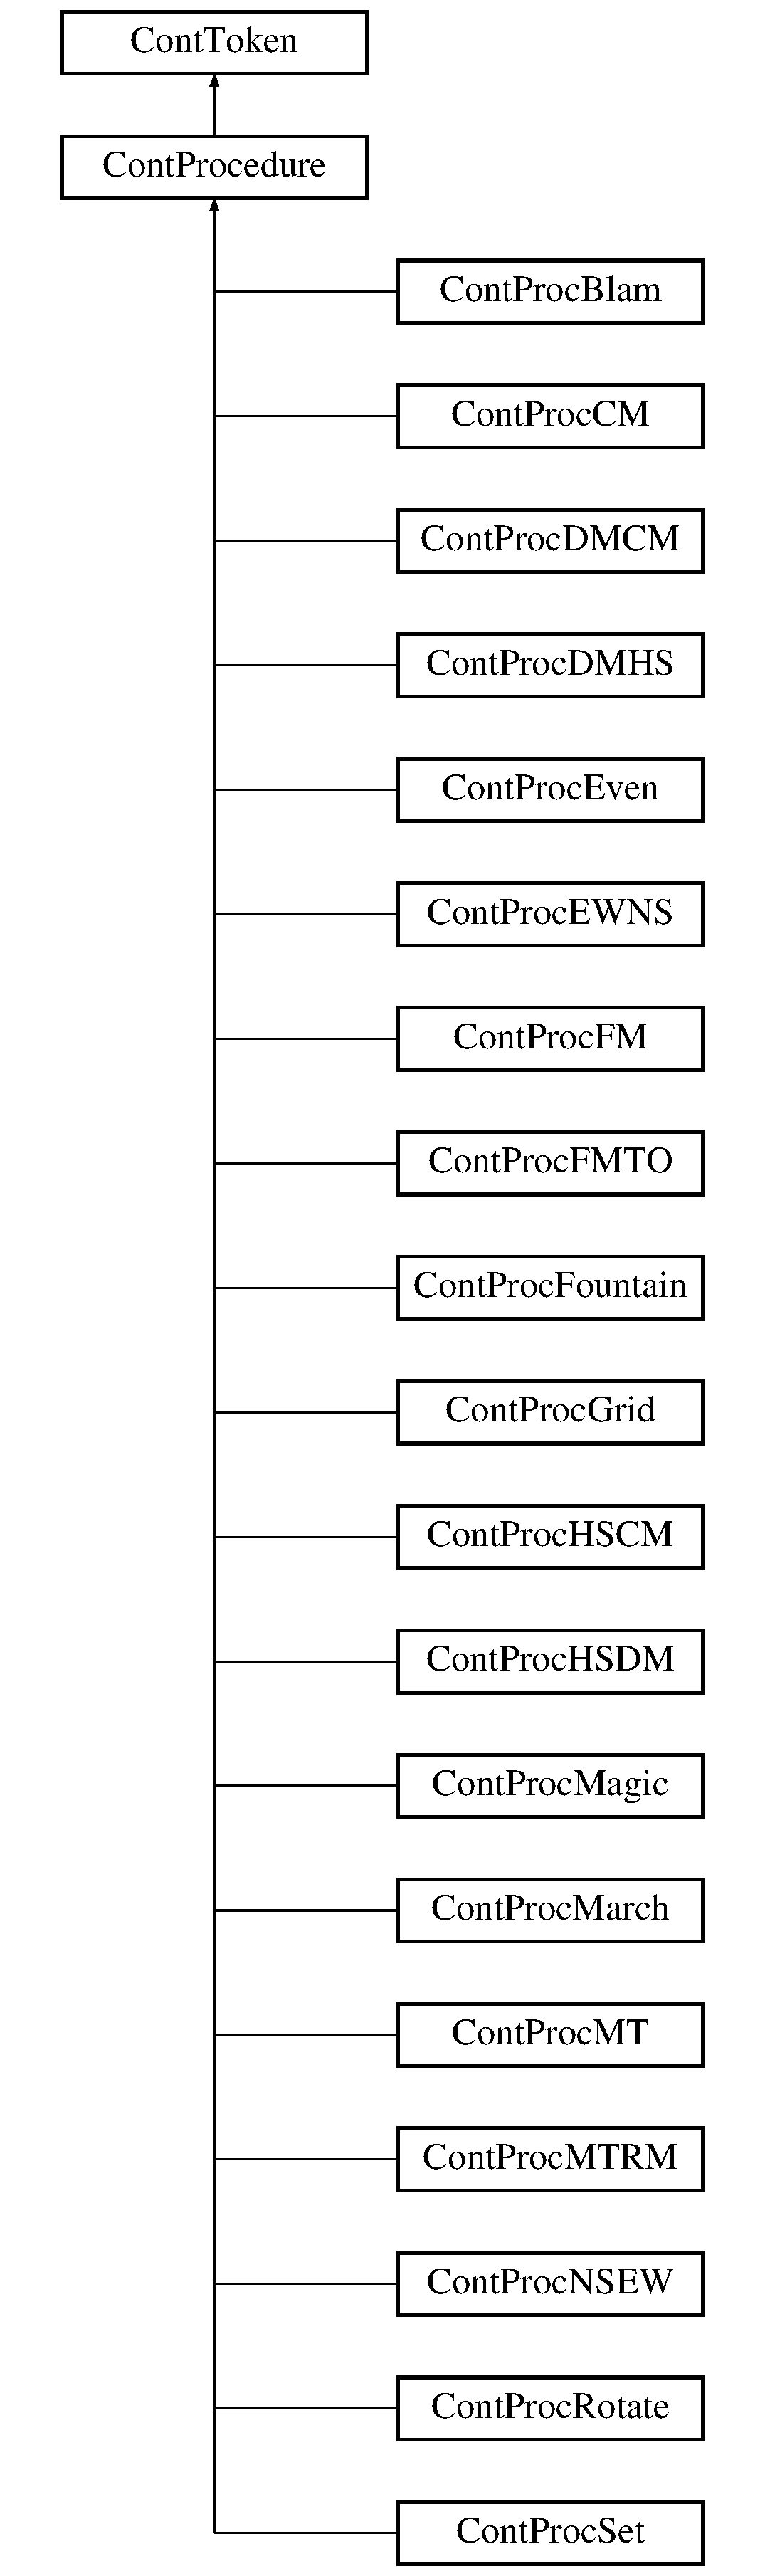
\includegraphics[height=12.000000cm]{a00067}
\end{center}
\end{figure}
\subsection*{Public Member Functions}
\begin{DoxyCompactItemize}
\item 
\hyperlink{a00067_a817bd84c2eac5073e90fed4000a190e0}{Cont\-Procedure} ()
\item 
virtual \hyperlink{a00067_a4d9a1ee6f37ad1885568e1a4d5ae2305}{$\sim$\-Cont\-Procedure} ()
\item 
virtual void \hyperlink{a00067_a7f7adefe250a00b3778669ef649f03ac}{Compile} (\hyperlink{a00007}{Animate\-Compile} $\ast$anim)=0
\end{DoxyCompactItemize}
\subsection*{Public Attributes}
\begin{DoxyCompactItemize}
\item 
\hyperlink{a00067}{Cont\-Procedure} $\ast$ \hyperlink{a00067_aac5b4a7edc2e4778ef7bb8dfed6ede8e}{next}
\end{DoxyCompactItemize}


\subsection{Constructor \& Destructor Documentation}
\hypertarget{a00067_a817bd84c2eac5073e90fed4000a190e0}{\index{Cont\-Procedure@{Cont\-Procedure}!Cont\-Procedure@{Cont\-Procedure}}
\index{Cont\-Procedure@{Cont\-Procedure}!ContProcedure@{Cont\-Procedure}}
\subsubsection[{Cont\-Procedure}]{\setlength{\rightskip}{0pt plus 5cm}Cont\-Procedure\-::\-Cont\-Procedure (
\begin{DoxyParamCaption}
{}
\end{DoxyParamCaption}
)\hspace{0.3cm}{\ttfamily [inline]}}}\label{a00067_a817bd84c2eac5073e90fed4000a190e0}
\hypertarget{a00067_a4d9a1ee6f37ad1885568e1a4d5ae2305}{\index{Cont\-Procedure@{Cont\-Procedure}!$\sim$\-Cont\-Procedure@{$\sim$\-Cont\-Procedure}}
\index{$\sim$\-Cont\-Procedure@{$\sim$\-Cont\-Procedure}!ContProcedure@{Cont\-Procedure}}
\subsubsection[{$\sim$\-Cont\-Procedure}]{\setlength{\rightskip}{0pt plus 5cm}Cont\-Procedure\-::$\sim$\-Cont\-Procedure (
\begin{DoxyParamCaption}
{}
\end{DoxyParamCaption}
)\hspace{0.3cm}{\ttfamily [virtual]}}}\label{a00067_a4d9a1ee6f37ad1885568e1a4d5ae2305}


\subsection{Member Function Documentation}
\hypertarget{a00067_a7f7adefe250a00b3778669ef649f03ac}{\index{Cont\-Procedure@{Cont\-Procedure}!Compile@{Compile}}
\index{Compile@{Compile}!ContProcedure@{Cont\-Procedure}}
\subsubsection[{Compile}]{\setlength{\rightskip}{0pt plus 5cm}virtual void Cont\-Procedure\-::\-Compile (
\begin{DoxyParamCaption}
\item[{{\bf Animate\-Compile} $\ast$}]{anim}
\end{DoxyParamCaption}
)\hspace{0.3cm}{\ttfamily [pure virtual]}}}\label{a00067_a7f7adefe250a00b3778669ef649f03ac}


Implemented in \hyperlink{a00081_a43308004b90299c4f06d4f7df29472ae}{Cont\-Proc\-Rotate}, \hyperlink{a00080_aa91db2ce7cb30ef776d9424f65c24db6}{Cont\-Proc\-N\-S\-E\-W}, \hyperlink{a00079_a7dbef5c4c51e4064a55efd9c3b4b8c45}{Cont\-Proc\-M\-T\-R\-M}, \hyperlink{a00078_a962aca7f48111ff35165fef9e30b7267}{Cont\-Proc\-M\-T}, \hyperlink{a00077_a98de0ad9854177887775bb191eb16ec4}{Cont\-Proc\-March}, \hyperlink{a00076_af65d4df561241982cdfda99425a6f42e}{Cont\-Proc\-Magic}, \hyperlink{a00075_acee31da94d32070ac68d5929c35851b4}{Cont\-Proc\-H\-S\-D\-M}, \hyperlink{a00074_ac601399766720bd99b7124dce80e91cf}{Cont\-Proc\-H\-S\-C\-M}, \hyperlink{a00073_a38f567fa3d7142ec6e5ca159e3a7a40d}{Cont\-Proc\-Grid}, \hyperlink{a00071_ae91ffc85c8a43412ee3164dd3c14be7d}{Cont\-Proc\-F\-M\-T\-O}, \hyperlink{a00070_afa13e90ef92926d841f8ccde4ffc28a6}{Cont\-Proc\-F\-M}, \hyperlink{a00072_a855a7fb74c148f0267862625fc4d3216}{Cont\-Proc\-Fountain}, \hyperlink{a00069_abf051788c6e6c552661a40f8179c11ee}{Cont\-Proc\-E\-W\-N\-S}, \hyperlink{a00068_afdf570f6d03a29b5743c4ecec8bbd416}{Cont\-Proc\-Even}, \hyperlink{a00066_aa12b04f473128f3d07139649ef944317}{Cont\-Proc\-D\-M\-H\-S}, \hyperlink{a00065_a90453323245d51cccd91dd50802e9f66}{Cont\-Proc\-D\-M\-C\-M}, \hyperlink{a00064_ae3d0ef74c8e17080072c537f29c17519}{Cont\-Proc\-C\-M}, \hyperlink{a00063_a049c64760a90035f4a4fadb1c190499e}{Cont\-Proc\-Blam}, and \hyperlink{a00082_a71bb8997d0068880ce828354ad0c8502}{Cont\-Proc\-Set}.



\subsection{Member Data Documentation}
\hypertarget{a00067_aac5b4a7edc2e4778ef7bb8dfed6ede8e}{\index{Cont\-Procedure@{Cont\-Procedure}!next@{next}}
\index{next@{next}!ContProcedure@{Cont\-Procedure}}
\subsubsection[{next}]{\setlength{\rightskip}{0pt plus 5cm}{\bf Cont\-Procedure}$\ast$ Cont\-Procedure\-::next}}\label{a00067_aac5b4a7edc2e4778ef7bb8dfed6ede8e}


The documentation for this class was generated from the following files\-:\begin{DoxyCompactItemize}
\item 
src/core/\hyperlink{a00218}{cont.\-h}\item 
src/core/\hyperlink{a00217}{cont.\-cpp}\end{DoxyCompactItemize}

\hypertarget{a00068}{\section{Cont\-Proc\-Even Class Reference}
\label{a00068}\index{Cont\-Proc\-Even@{Cont\-Proc\-Even}}
}


{\ttfamily \#include $<$cont.\-h$>$}

Inheritance diagram for Cont\-Proc\-Even\-:\begin{figure}[H]
\begin{center}
\leavevmode
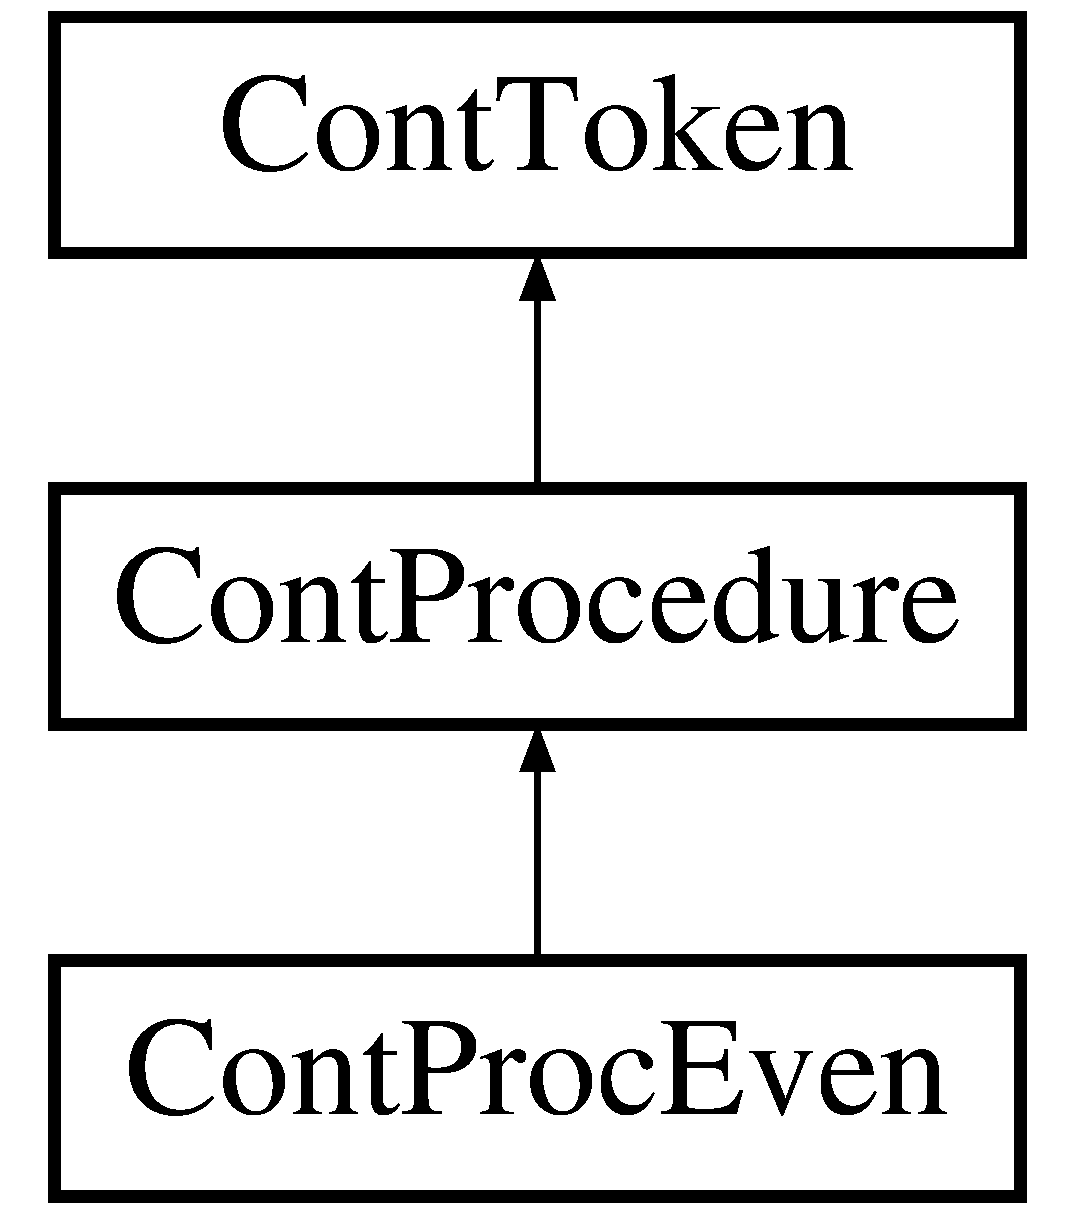
\includegraphics[height=3.000000cm]{a00068}
\end{center}
\end{figure}
\subsection*{Public Member Functions}
\begin{DoxyCompactItemize}
\item 
\hyperlink{a00068_afdb53d03002a8103359eefd4c8a69d8f}{Cont\-Proc\-Even} (\hyperlink{a00086}{Cont\-Value} $\ast$steps, \hyperlink{a00062}{Cont\-Point} $\ast$p)
\item 
virtual \hyperlink{a00068_a0c6ba8bbe36a81154d3290ab56682a44}{$\sim$\-Cont\-Proc\-Even} ()
\item 
virtual void \hyperlink{a00068_afdf570f6d03a29b5743c4ecec8bbd416}{Compile} (\hyperlink{a00007}{Animate\-Compile} $\ast$anim)
\end{DoxyCompactItemize}
\subsection*{Private Attributes}
\begin{DoxyCompactItemize}
\item 
\hyperlink{a00086}{Cont\-Value} $\ast$ \hyperlink{a00068_aa05efb6bad22228ea0d6e7234f2f7b4f}{stps}
\item 
\hyperlink{a00062}{Cont\-Point} $\ast$ \hyperlink{a00068_a5f29bd5f2ada87f5b657f8494ed36afa}{pnt}
\end{DoxyCompactItemize}
\subsection*{Additional Inherited Members}


\subsection{Constructor \& Destructor Documentation}
\hypertarget{a00068_afdb53d03002a8103359eefd4c8a69d8f}{\index{Cont\-Proc\-Even@{Cont\-Proc\-Even}!Cont\-Proc\-Even@{Cont\-Proc\-Even}}
\index{Cont\-Proc\-Even@{Cont\-Proc\-Even}!ContProcEven@{Cont\-Proc\-Even}}
\subsubsection[{Cont\-Proc\-Even}]{\setlength{\rightskip}{0pt plus 5cm}Cont\-Proc\-Even\-::\-Cont\-Proc\-Even (
\begin{DoxyParamCaption}
\item[{{\bf Cont\-Value} $\ast$}]{steps, }
\item[{{\bf Cont\-Point} $\ast$}]{p}
\end{DoxyParamCaption}
)\hspace{0.3cm}{\ttfamily [inline]}}}\label{a00068_afdb53d03002a8103359eefd4c8a69d8f}
\hypertarget{a00068_a0c6ba8bbe36a81154d3290ab56682a44}{\index{Cont\-Proc\-Even@{Cont\-Proc\-Even}!$\sim$\-Cont\-Proc\-Even@{$\sim$\-Cont\-Proc\-Even}}
\index{$\sim$\-Cont\-Proc\-Even@{$\sim$\-Cont\-Proc\-Even}!ContProcEven@{Cont\-Proc\-Even}}
\subsubsection[{$\sim$\-Cont\-Proc\-Even}]{\setlength{\rightskip}{0pt plus 5cm}Cont\-Proc\-Even\-::$\sim$\-Cont\-Proc\-Even (
\begin{DoxyParamCaption}
{}
\end{DoxyParamCaption}
)\hspace{0.3cm}{\ttfamily [virtual]}}}\label{a00068_a0c6ba8bbe36a81154d3290ab56682a44}


\subsection{Member Function Documentation}
\hypertarget{a00068_afdf570f6d03a29b5743c4ecec8bbd416}{\index{Cont\-Proc\-Even@{Cont\-Proc\-Even}!Compile@{Compile}}
\index{Compile@{Compile}!ContProcEven@{Cont\-Proc\-Even}}
\subsubsection[{Compile}]{\setlength{\rightskip}{0pt plus 5cm}void Cont\-Proc\-Even\-::\-Compile (
\begin{DoxyParamCaption}
\item[{{\bf Animate\-Compile} $\ast$}]{anim}
\end{DoxyParamCaption}
)\hspace{0.3cm}{\ttfamily [virtual]}}}\label{a00068_afdf570f6d03a29b5743c4ecec8bbd416}


Implements \hyperlink{a00067_a7f7adefe250a00b3778669ef649f03ac}{Cont\-Procedure}.



\subsection{Member Data Documentation}
\hypertarget{a00068_a5f29bd5f2ada87f5b657f8494ed36afa}{\index{Cont\-Proc\-Even@{Cont\-Proc\-Even}!pnt@{pnt}}
\index{pnt@{pnt}!ContProcEven@{Cont\-Proc\-Even}}
\subsubsection[{pnt}]{\setlength{\rightskip}{0pt plus 5cm}{\bf Cont\-Point}$\ast$ Cont\-Proc\-Even\-::pnt\hspace{0.3cm}{\ttfamily [private]}}}\label{a00068_a5f29bd5f2ada87f5b657f8494ed36afa}
\hypertarget{a00068_aa05efb6bad22228ea0d6e7234f2f7b4f}{\index{Cont\-Proc\-Even@{Cont\-Proc\-Even}!stps@{stps}}
\index{stps@{stps}!ContProcEven@{Cont\-Proc\-Even}}
\subsubsection[{stps}]{\setlength{\rightskip}{0pt plus 5cm}{\bf Cont\-Value}$\ast$ Cont\-Proc\-Even\-::stps\hspace{0.3cm}{\ttfamily [private]}}}\label{a00068_aa05efb6bad22228ea0d6e7234f2f7b4f}


The documentation for this class was generated from the following files\-:\begin{DoxyCompactItemize}
\item 
src/core/\hyperlink{a00218}{cont.\-h}\item 
src/core/\hyperlink{a00217}{cont.\-cpp}\end{DoxyCompactItemize}

\hypertarget{a00069}{\section{Cont\-Proc\-E\-W\-N\-S Class Reference}
\label{a00069}\index{Cont\-Proc\-E\-W\-N\-S@{Cont\-Proc\-E\-W\-N\-S}}
}


{\ttfamily \#include $<$cont.\-h$>$}

Inheritance diagram for Cont\-Proc\-E\-W\-N\-S\-:\begin{figure}[H]
\begin{center}
\leavevmode
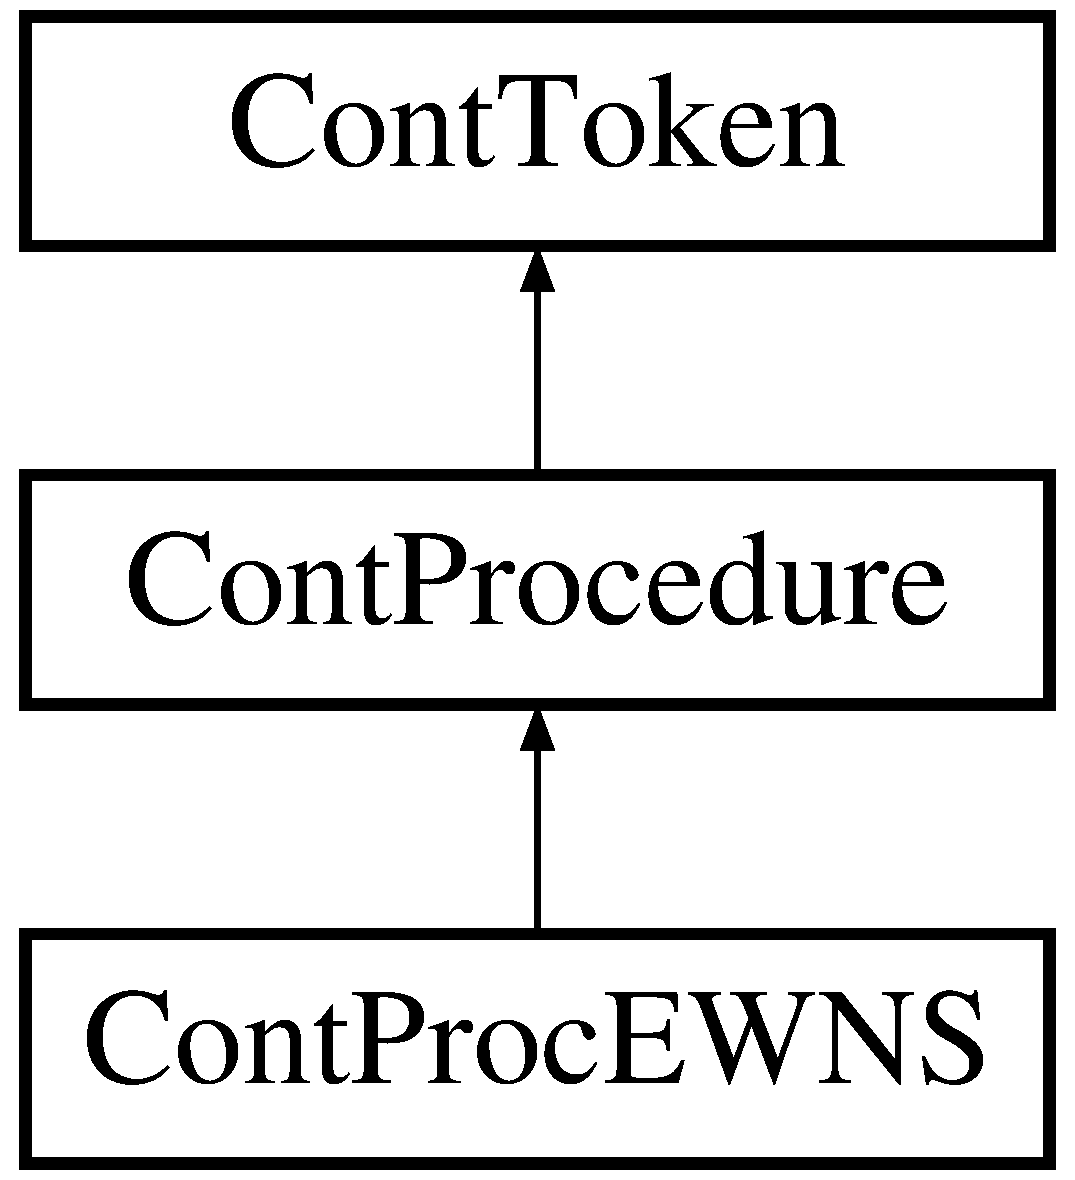
\includegraphics[height=3.000000cm]{a00069}
\end{center}
\end{figure}
\subsection*{Public Member Functions}
\begin{DoxyCompactItemize}
\item 
\hyperlink{a00069_a8fe73f6c99ec2b7e4fa1d16b9777cd88}{Cont\-Proc\-E\-W\-N\-S} (\hyperlink{a00062}{Cont\-Point} $\ast$p)
\item 
virtual \hyperlink{a00069_ab3b2c3219f33f940cbe26ace3f4962b0}{$\sim$\-Cont\-Proc\-E\-W\-N\-S} ()
\item 
virtual void \hyperlink{a00069_abf051788c6e6c552661a40f8179c11ee}{Compile} (\hyperlink{a00007}{Animate\-Compile} $\ast$anim)
\end{DoxyCompactItemize}
\subsection*{Private Attributes}
\begin{DoxyCompactItemize}
\item 
\hyperlink{a00062}{Cont\-Point} $\ast$ \hyperlink{a00069_a8fbfa9a491ffb84d2786b78d7dd76004}{pnt}
\end{DoxyCompactItemize}
\subsection*{Additional Inherited Members}


\subsection{Constructor \& Destructor Documentation}
\hypertarget{a00069_a8fe73f6c99ec2b7e4fa1d16b9777cd88}{\index{Cont\-Proc\-E\-W\-N\-S@{Cont\-Proc\-E\-W\-N\-S}!Cont\-Proc\-E\-W\-N\-S@{Cont\-Proc\-E\-W\-N\-S}}
\index{Cont\-Proc\-E\-W\-N\-S@{Cont\-Proc\-E\-W\-N\-S}!ContProcEWNS@{Cont\-Proc\-E\-W\-N\-S}}
\subsubsection[{Cont\-Proc\-E\-W\-N\-S}]{\setlength{\rightskip}{0pt plus 5cm}Cont\-Proc\-E\-W\-N\-S\-::\-Cont\-Proc\-E\-W\-N\-S (
\begin{DoxyParamCaption}
\item[{{\bf Cont\-Point} $\ast$}]{p}
\end{DoxyParamCaption}
)\hspace{0.3cm}{\ttfamily [inline]}}}\label{a00069_a8fe73f6c99ec2b7e4fa1d16b9777cd88}
\hypertarget{a00069_ab3b2c3219f33f940cbe26ace3f4962b0}{\index{Cont\-Proc\-E\-W\-N\-S@{Cont\-Proc\-E\-W\-N\-S}!$\sim$\-Cont\-Proc\-E\-W\-N\-S@{$\sim$\-Cont\-Proc\-E\-W\-N\-S}}
\index{$\sim$\-Cont\-Proc\-E\-W\-N\-S@{$\sim$\-Cont\-Proc\-E\-W\-N\-S}!ContProcEWNS@{Cont\-Proc\-E\-W\-N\-S}}
\subsubsection[{$\sim$\-Cont\-Proc\-E\-W\-N\-S}]{\setlength{\rightskip}{0pt plus 5cm}Cont\-Proc\-E\-W\-N\-S\-::$\sim$\-Cont\-Proc\-E\-W\-N\-S (
\begin{DoxyParamCaption}
{}
\end{DoxyParamCaption}
)\hspace{0.3cm}{\ttfamily [virtual]}}}\label{a00069_ab3b2c3219f33f940cbe26ace3f4962b0}


\subsection{Member Function Documentation}
\hypertarget{a00069_abf051788c6e6c552661a40f8179c11ee}{\index{Cont\-Proc\-E\-W\-N\-S@{Cont\-Proc\-E\-W\-N\-S}!Compile@{Compile}}
\index{Compile@{Compile}!ContProcEWNS@{Cont\-Proc\-E\-W\-N\-S}}
\subsubsection[{Compile}]{\setlength{\rightskip}{0pt plus 5cm}void Cont\-Proc\-E\-W\-N\-S\-::\-Compile (
\begin{DoxyParamCaption}
\item[{{\bf Animate\-Compile} $\ast$}]{anim}
\end{DoxyParamCaption}
)\hspace{0.3cm}{\ttfamily [virtual]}}}\label{a00069_abf051788c6e6c552661a40f8179c11ee}


Implements \hyperlink{a00067_a7f7adefe250a00b3778669ef649f03ac}{Cont\-Procedure}.



\subsection{Member Data Documentation}
\hypertarget{a00069_a8fbfa9a491ffb84d2786b78d7dd76004}{\index{Cont\-Proc\-E\-W\-N\-S@{Cont\-Proc\-E\-W\-N\-S}!pnt@{pnt}}
\index{pnt@{pnt}!ContProcEWNS@{Cont\-Proc\-E\-W\-N\-S}}
\subsubsection[{pnt}]{\setlength{\rightskip}{0pt plus 5cm}{\bf Cont\-Point}$\ast$ Cont\-Proc\-E\-W\-N\-S\-::pnt\hspace{0.3cm}{\ttfamily [private]}}}\label{a00069_a8fbfa9a491ffb84d2786b78d7dd76004}


The documentation for this class was generated from the following files\-:\begin{DoxyCompactItemize}
\item 
src/core/\hyperlink{a00218}{cont.\-h}\item 
src/core/\hyperlink{a00217}{cont.\-cpp}\end{DoxyCompactItemize}

\hypertarget{a00070}{\section{Cont\-Proc\-F\-M Class Reference}
\label{a00070}\index{Cont\-Proc\-F\-M@{Cont\-Proc\-F\-M}}
}


{\ttfamily \#include $<$cont.\-h$>$}

Inheritance diagram for Cont\-Proc\-F\-M\-:\begin{figure}[H]
\begin{center}
\leavevmode
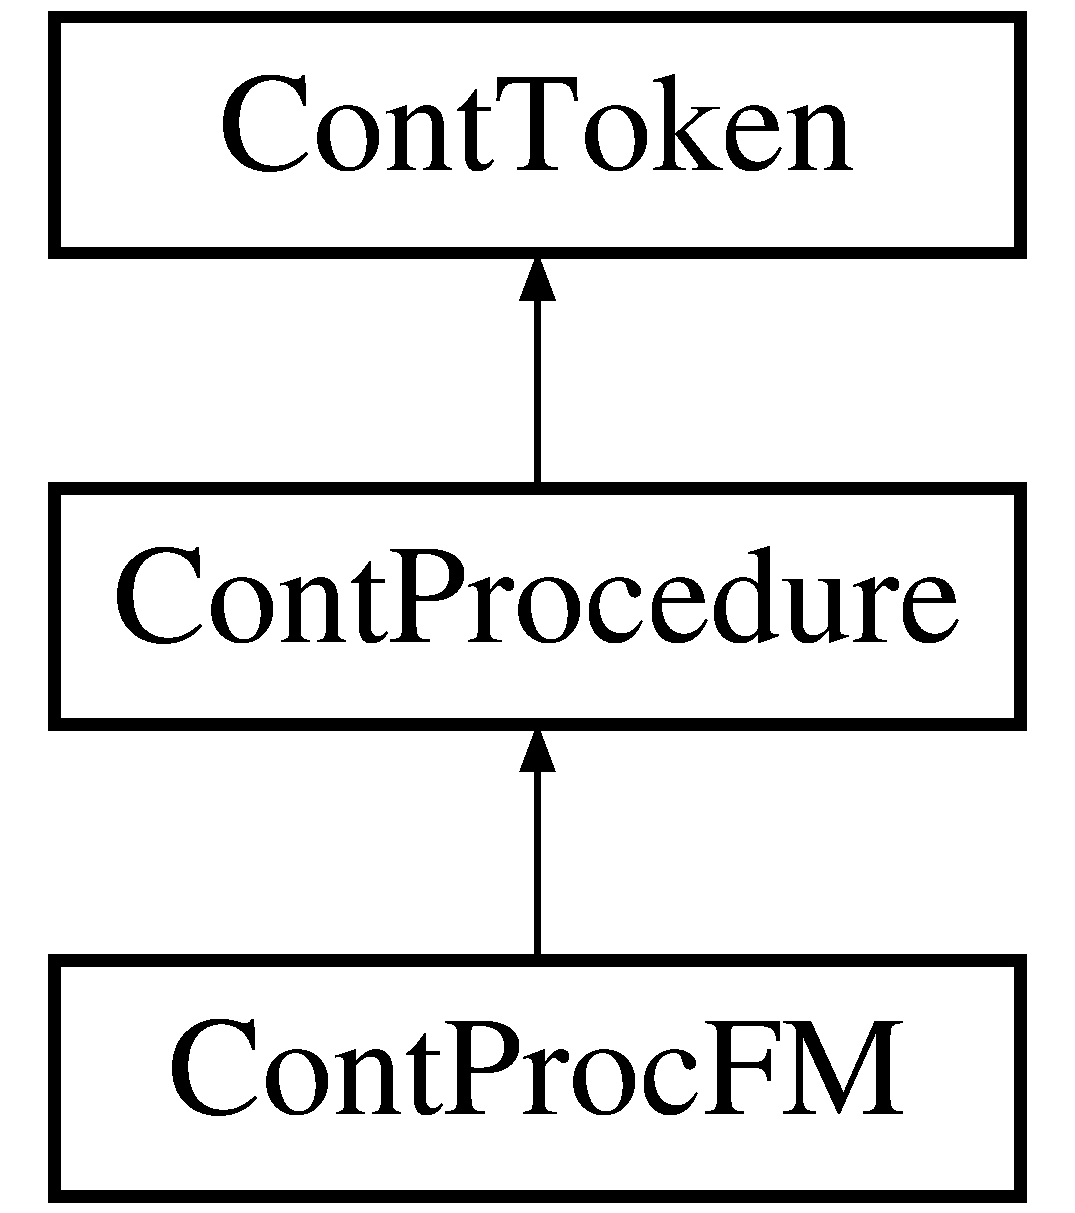
\includegraphics[height=3.000000cm]{a00070}
\end{center}
\end{figure}
\subsection*{Public Member Functions}
\begin{DoxyCompactItemize}
\item 
\hyperlink{a00070_abff5e5744bc965d792aae3c410c33e77}{Cont\-Proc\-F\-M} (\hyperlink{a00086}{Cont\-Value} $\ast$steps, \hyperlink{a00086}{Cont\-Value} $\ast$d)
\item 
virtual \hyperlink{a00070_a208c5853dba2562b250db21bc81e21b6}{$\sim$\-Cont\-Proc\-F\-M} ()
\item 
virtual void \hyperlink{a00070_afa13e90ef92926d841f8ccde4ffc28a6}{Compile} (\hyperlink{a00007}{Animate\-Compile} $\ast$anim)
\end{DoxyCompactItemize}
\subsection*{Private Attributes}
\begin{DoxyCompactItemize}
\item 
\hyperlink{a00086}{Cont\-Value} $\ast$ \hyperlink{a00070_aeb044fa5c2acb27c72c017fcd41d09ce}{stps}
\item 
\hyperlink{a00086}{Cont\-Value} $\ast$ \hyperlink{a00070_a2a5343eff6f4bb803adf4adb9e222e12}{dir}
\end{DoxyCompactItemize}
\subsection*{Additional Inherited Members}


\subsection{Constructor \& Destructor Documentation}
\hypertarget{a00070_abff5e5744bc965d792aae3c410c33e77}{\index{Cont\-Proc\-F\-M@{Cont\-Proc\-F\-M}!Cont\-Proc\-F\-M@{Cont\-Proc\-F\-M}}
\index{Cont\-Proc\-F\-M@{Cont\-Proc\-F\-M}!ContProcFM@{Cont\-Proc\-F\-M}}
\subsubsection[{Cont\-Proc\-F\-M}]{\setlength{\rightskip}{0pt plus 5cm}Cont\-Proc\-F\-M\-::\-Cont\-Proc\-F\-M (
\begin{DoxyParamCaption}
\item[{{\bf Cont\-Value} $\ast$}]{steps, }
\item[{{\bf Cont\-Value} $\ast$}]{d}
\end{DoxyParamCaption}
)\hspace{0.3cm}{\ttfamily [inline]}}}\label{a00070_abff5e5744bc965d792aae3c410c33e77}
\hypertarget{a00070_a208c5853dba2562b250db21bc81e21b6}{\index{Cont\-Proc\-F\-M@{Cont\-Proc\-F\-M}!$\sim$\-Cont\-Proc\-F\-M@{$\sim$\-Cont\-Proc\-F\-M}}
\index{$\sim$\-Cont\-Proc\-F\-M@{$\sim$\-Cont\-Proc\-F\-M}!ContProcFM@{Cont\-Proc\-F\-M}}
\subsubsection[{$\sim$\-Cont\-Proc\-F\-M}]{\setlength{\rightskip}{0pt plus 5cm}Cont\-Proc\-F\-M\-::$\sim$\-Cont\-Proc\-F\-M (
\begin{DoxyParamCaption}
{}
\end{DoxyParamCaption}
)\hspace{0.3cm}{\ttfamily [virtual]}}}\label{a00070_a208c5853dba2562b250db21bc81e21b6}


\subsection{Member Function Documentation}
\hypertarget{a00070_afa13e90ef92926d841f8ccde4ffc28a6}{\index{Cont\-Proc\-F\-M@{Cont\-Proc\-F\-M}!Compile@{Compile}}
\index{Compile@{Compile}!ContProcFM@{Cont\-Proc\-F\-M}}
\subsubsection[{Compile}]{\setlength{\rightskip}{0pt plus 5cm}void Cont\-Proc\-F\-M\-::\-Compile (
\begin{DoxyParamCaption}
\item[{{\bf Animate\-Compile} $\ast$}]{anim}
\end{DoxyParamCaption}
)\hspace{0.3cm}{\ttfamily [virtual]}}}\label{a00070_afa13e90ef92926d841f8ccde4ffc28a6}


Implements \hyperlink{a00067_a7f7adefe250a00b3778669ef649f03ac}{Cont\-Procedure}.



\subsection{Member Data Documentation}
\hypertarget{a00070_a2a5343eff6f4bb803adf4adb9e222e12}{\index{Cont\-Proc\-F\-M@{Cont\-Proc\-F\-M}!dir@{dir}}
\index{dir@{dir}!ContProcFM@{Cont\-Proc\-F\-M}}
\subsubsection[{dir}]{\setlength{\rightskip}{0pt plus 5cm}{\bf Cont\-Value} $\ast$ Cont\-Proc\-F\-M\-::dir\hspace{0.3cm}{\ttfamily [private]}}}\label{a00070_a2a5343eff6f4bb803adf4adb9e222e12}
\hypertarget{a00070_aeb044fa5c2acb27c72c017fcd41d09ce}{\index{Cont\-Proc\-F\-M@{Cont\-Proc\-F\-M}!stps@{stps}}
\index{stps@{stps}!ContProcFM@{Cont\-Proc\-F\-M}}
\subsubsection[{stps}]{\setlength{\rightskip}{0pt plus 5cm}{\bf Cont\-Value}$\ast$ Cont\-Proc\-F\-M\-::stps\hspace{0.3cm}{\ttfamily [private]}}}\label{a00070_aeb044fa5c2acb27c72c017fcd41d09ce}


The documentation for this class was generated from the following files\-:\begin{DoxyCompactItemize}
\item 
src/core/\hyperlink{a00218}{cont.\-h}\item 
src/core/\hyperlink{a00217}{cont.\-cpp}\end{DoxyCompactItemize}

\hypertarget{a00071}{\section{Cont\-Proc\-F\-M\-T\-O Class Reference}
\label{a00071}\index{Cont\-Proc\-F\-M\-T\-O@{Cont\-Proc\-F\-M\-T\-O}}
}


{\ttfamily \#include $<$cont.\-h$>$}

Inheritance diagram for Cont\-Proc\-F\-M\-T\-O\-:\begin{figure}[H]
\begin{center}
\leavevmode
\includegraphics[height=3.000000cm]{a00071}
\end{center}
\end{figure}
\subsection*{Public Member Functions}
\begin{DoxyCompactItemize}
\item 
\hyperlink{a00071_a10727448ea9cb40eec436b7abe2d4675}{Cont\-Proc\-F\-M\-T\-O} (\hyperlink{a00062}{Cont\-Point} $\ast$p)
\item 
virtual \hyperlink{a00071_a4f17ce279104980b43974e4f953b6d9a}{$\sim$\-Cont\-Proc\-F\-M\-T\-O} ()
\item 
virtual void \hyperlink{a00071_ae91ffc85c8a43412ee3164dd3c14be7d}{Compile} (\hyperlink{a00007}{Animate\-Compile} $\ast$anim)
\end{DoxyCompactItemize}
\subsection*{Private Attributes}
\begin{DoxyCompactItemize}
\item 
\hyperlink{a00062}{Cont\-Point} $\ast$ \hyperlink{a00071_aa39384486319e7ed072a35c1cbe6647b}{pnt}
\end{DoxyCompactItemize}
\subsection*{Additional Inherited Members}


\subsection{Constructor \& Destructor Documentation}
\hypertarget{a00071_a10727448ea9cb40eec436b7abe2d4675}{\index{Cont\-Proc\-F\-M\-T\-O@{Cont\-Proc\-F\-M\-T\-O}!Cont\-Proc\-F\-M\-T\-O@{Cont\-Proc\-F\-M\-T\-O}}
\index{Cont\-Proc\-F\-M\-T\-O@{Cont\-Proc\-F\-M\-T\-O}!ContProcFMTO@{Cont\-Proc\-F\-M\-T\-O}}
\subsubsection[{Cont\-Proc\-F\-M\-T\-O}]{\setlength{\rightskip}{0pt plus 5cm}Cont\-Proc\-F\-M\-T\-O\-::\-Cont\-Proc\-F\-M\-T\-O (
\begin{DoxyParamCaption}
\item[{{\bf Cont\-Point} $\ast$}]{p}
\end{DoxyParamCaption}
)\hspace{0.3cm}{\ttfamily [inline]}}}\label{a00071_a10727448ea9cb40eec436b7abe2d4675}
\hypertarget{a00071_a4f17ce279104980b43974e4f953b6d9a}{\index{Cont\-Proc\-F\-M\-T\-O@{Cont\-Proc\-F\-M\-T\-O}!$\sim$\-Cont\-Proc\-F\-M\-T\-O@{$\sim$\-Cont\-Proc\-F\-M\-T\-O}}
\index{$\sim$\-Cont\-Proc\-F\-M\-T\-O@{$\sim$\-Cont\-Proc\-F\-M\-T\-O}!ContProcFMTO@{Cont\-Proc\-F\-M\-T\-O}}
\subsubsection[{$\sim$\-Cont\-Proc\-F\-M\-T\-O}]{\setlength{\rightskip}{0pt plus 5cm}Cont\-Proc\-F\-M\-T\-O\-::$\sim$\-Cont\-Proc\-F\-M\-T\-O (
\begin{DoxyParamCaption}
{}
\end{DoxyParamCaption}
)\hspace{0.3cm}{\ttfamily [virtual]}}}\label{a00071_a4f17ce279104980b43974e4f953b6d9a}


\subsection{Member Function Documentation}
\hypertarget{a00071_ae91ffc85c8a43412ee3164dd3c14be7d}{\index{Cont\-Proc\-F\-M\-T\-O@{Cont\-Proc\-F\-M\-T\-O}!Compile@{Compile}}
\index{Compile@{Compile}!ContProcFMTO@{Cont\-Proc\-F\-M\-T\-O}}
\subsubsection[{Compile}]{\setlength{\rightskip}{0pt plus 5cm}void Cont\-Proc\-F\-M\-T\-O\-::\-Compile (
\begin{DoxyParamCaption}
\item[{{\bf Animate\-Compile} $\ast$}]{anim}
\end{DoxyParamCaption}
)\hspace{0.3cm}{\ttfamily [virtual]}}}\label{a00071_ae91ffc85c8a43412ee3164dd3c14be7d}


Implements \hyperlink{a00067_a7f7adefe250a00b3778669ef649f03ac}{Cont\-Procedure}.



\subsection{Member Data Documentation}
\hypertarget{a00071_aa39384486319e7ed072a35c1cbe6647b}{\index{Cont\-Proc\-F\-M\-T\-O@{Cont\-Proc\-F\-M\-T\-O}!pnt@{pnt}}
\index{pnt@{pnt}!ContProcFMTO@{Cont\-Proc\-F\-M\-T\-O}}
\subsubsection[{pnt}]{\setlength{\rightskip}{0pt plus 5cm}{\bf Cont\-Point}$\ast$ Cont\-Proc\-F\-M\-T\-O\-::pnt\hspace{0.3cm}{\ttfamily [private]}}}\label{a00071_aa39384486319e7ed072a35c1cbe6647b}


The documentation for this class was generated from the following files\-:\begin{DoxyCompactItemize}
\item 
src/core/\hyperlink{a00218}{cont.\-h}\item 
src/core/\hyperlink{a00217}{cont.\-cpp}\end{DoxyCompactItemize}

\hypertarget{a00072}{\section{Cont\-Proc\-Fountain Class Reference}
\label{a00072}\index{Cont\-Proc\-Fountain@{Cont\-Proc\-Fountain}}
}


{\ttfamily \#include $<$cont.\-h$>$}

Inheritance diagram for Cont\-Proc\-Fountain\-:\begin{figure}[H]
\begin{center}
\leavevmode
\includegraphics[height=3.000000cm]{a00072}
\end{center}
\end{figure}
\subsection*{Public Member Functions}
\begin{DoxyCompactItemize}
\item 
\hyperlink{a00072_aca2c6b542c6c785b923a46e098036ace}{Cont\-Proc\-Fountain} (\hyperlink{a00086}{Cont\-Value} $\ast$d1, \hyperlink{a00086}{Cont\-Value} $\ast$d2, \hyperlink{a00086}{Cont\-Value} $\ast$s1, \hyperlink{a00086}{Cont\-Value} $\ast$s2, \hyperlink{a00062}{Cont\-Point} $\ast$p)
\item 
virtual \hyperlink{a00072_ac740967b07c7b5dfced9cae62d0410fc}{$\sim$\-Cont\-Proc\-Fountain} ()
\item 
virtual void \hyperlink{a00072_a855a7fb74c148f0267862625fc4d3216}{Compile} (\hyperlink{a00007}{Animate\-Compile} $\ast$anim)
\end{DoxyCompactItemize}
\subsection*{Private Attributes}
\begin{DoxyCompactItemize}
\item 
\hyperlink{a00086}{Cont\-Value} $\ast$ \hyperlink{a00072_aef7f3257c44eb70b6a6a7cb84ce145b2}{dir1}
\item 
\hyperlink{a00086}{Cont\-Value} $\ast$ \hyperlink{a00072_ab6177ddc4540a0d5e987b317955e5f2c}{dir2}
\item 
\hyperlink{a00086}{Cont\-Value} $\ast$ \hyperlink{a00072_aecf7f8806b9d5d8c0ee60df2afe76a56}{stepsize1}
\item 
\hyperlink{a00086}{Cont\-Value} $\ast$ \hyperlink{a00072_a230a7d97b18971908811d5b2f920d4e0}{stepsize2}
\item 
\hyperlink{a00062}{Cont\-Point} $\ast$ \hyperlink{a00072_aa201aa8879ac43945d68aa669aa4a3ff}{pnt}
\end{DoxyCompactItemize}
\subsection*{Additional Inherited Members}


\subsection{Constructor \& Destructor Documentation}
\hypertarget{a00072_aca2c6b542c6c785b923a46e098036ace}{\index{Cont\-Proc\-Fountain@{Cont\-Proc\-Fountain}!Cont\-Proc\-Fountain@{Cont\-Proc\-Fountain}}
\index{Cont\-Proc\-Fountain@{Cont\-Proc\-Fountain}!ContProcFountain@{Cont\-Proc\-Fountain}}
\subsubsection[{Cont\-Proc\-Fountain}]{\setlength{\rightskip}{0pt plus 5cm}Cont\-Proc\-Fountain\-::\-Cont\-Proc\-Fountain (
\begin{DoxyParamCaption}
\item[{{\bf Cont\-Value} $\ast$}]{d1, }
\item[{{\bf Cont\-Value} $\ast$}]{d2, }
\item[{{\bf Cont\-Value} $\ast$}]{s1, }
\item[{{\bf Cont\-Value} $\ast$}]{s2, }
\item[{{\bf Cont\-Point} $\ast$}]{p}
\end{DoxyParamCaption}
)\hspace{0.3cm}{\ttfamily [inline]}}}\label{a00072_aca2c6b542c6c785b923a46e098036ace}
\hypertarget{a00072_ac740967b07c7b5dfced9cae62d0410fc}{\index{Cont\-Proc\-Fountain@{Cont\-Proc\-Fountain}!$\sim$\-Cont\-Proc\-Fountain@{$\sim$\-Cont\-Proc\-Fountain}}
\index{$\sim$\-Cont\-Proc\-Fountain@{$\sim$\-Cont\-Proc\-Fountain}!ContProcFountain@{Cont\-Proc\-Fountain}}
\subsubsection[{$\sim$\-Cont\-Proc\-Fountain}]{\setlength{\rightskip}{0pt plus 5cm}Cont\-Proc\-Fountain\-::$\sim$\-Cont\-Proc\-Fountain (
\begin{DoxyParamCaption}
{}
\end{DoxyParamCaption}
)\hspace{0.3cm}{\ttfamily [virtual]}}}\label{a00072_ac740967b07c7b5dfced9cae62d0410fc}


\subsection{Member Function Documentation}
\hypertarget{a00072_a855a7fb74c148f0267862625fc4d3216}{\index{Cont\-Proc\-Fountain@{Cont\-Proc\-Fountain}!Compile@{Compile}}
\index{Compile@{Compile}!ContProcFountain@{Cont\-Proc\-Fountain}}
\subsubsection[{Compile}]{\setlength{\rightskip}{0pt plus 5cm}void Cont\-Proc\-Fountain\-::\-Compile (
\begin{DoxyParamCaption}
\item[{{\bf Animate\-Compile} $\ast$}]{anim}
\end{DoxyParamCaption}
)\hspace{0.3cm}{\ttfamily [virtual]}}}\label{a00072_a855a7fb74c148f0267862625fc4d3216}


Implements \hyperlink{a00067_a7f7adefe250a00b3778669ef649f03ac}{Cont\-Procedure}.



\subsection{Member Data Documentation}
\hypertarget{a00072_aef7f3257c44eb70b6a6a7cb84ce145b2}{\index{Cont\-Proc\-Fountain@{Cont\-Proc\-Fountain}!dir1@{dir1}}
\index{dir1@{dir1}!ContProcFountain@{Cont\-Proc\-Fountain}}
\subsubsection[{dir1}]{\setlength{\rightskip}{0pt plus 5cm}{\bf Cont\-Value}$\ast$ Cont\-Proc\-Fountain\-::dir1\hspace{0.3cm}{\ttfamily [private]}}}\label{a00072_aef7f3257c44eb70b6a6a7cb84ce145b2}
\hypertarget{a00072_ab6177ddc4540a0d5e987b317955e5f2c}{\index{Cont\-Proc\-Fountain@{Cont\-Proc\-Fountain}!dir2@{dir2}}
\index{dir2@{dir2}!ContProcFountain@{Cont\-Proc\-Fountain}}
\subsubsection[{dir2}]{\setlength{\rightskip}{0pt plus 5cm}{\bf Cont\-Value} $\ast$ Cont\-Proc\-Fountain\-::dir2\hspace{0.3cm}{\ttfamily [private]}}}\label{a00072_ab6177ddc4540a0d5e987b317955e5f2c}
\hypertarget{a00072_aa201aa8879ac43945d68aa669aa4a3ff}{\index{Cont\-Proc\-Fountain@{Cont\-Proc\-Fountain}!pnt@{pnt}}
\index{pnt@{pnt}!ContProcFountain@{Cont\-Proc\-Fountain}}
\subsubsection[{pnt}]{\setlength{\rightskip}{0pt plus 5cm}{\bf Cont\-Point}$\ast$ Cont\-Proc\-Fountain\-::pnt\hspace{0.3cm}{\ttfamily [private]}}}\label{a00072_aa201aa8879ac43945d68aa669aa4a3ff}
\hypertarget{a00072_aecf7f8806b9d5d8c0ee60df2afe76a56}{\index{Cont\-Proc\-Fountain@{Cont\-Proc\-Fountain}!stepsize1@{stepsize1}}
\index{stepsize1@{stepsize1}!ContProcFountain@{Cont\-Proc\-Fountain}}
\subsubsection[{stepsize1}]{\setlength{\rightskip}{0pt plus 5cm}{\bf Cont\-Value}$\ast$ Cont\-Proc\-Fountain\-::stepsize1\hspace{0.3cm}{\ttfamily [private]}}}\label{a00072_aecf7f8806b9d5d8c0ee60df2afe76a56}
\hypertarget{a00072_a230a7d97b18971908811d5b2f920d4e0}{\index{Cont\-Proc\-Fountain@{Cont\-Proc\-Fountain}!stepsize2@{stepsize2}}
\index{stepsize2@{stepsize2}!ContProcFountain@{Cont\-Proc\-Fountain}}
\subsubsection[{stepsize2}]{\setlength{\rightskip}{0pt plus 5cm}{\bf Cont\-Value} $\ast$ Cont\-Proc\-Fountain\-::stepsize2\hspace{0.3cm}{\ttfamily [private]}}}\label{a00072_a230a7d97b18971908811d5b2f920d4e0}


The documentation for this class was generated from the following files\-:\begin{DoxyCompactItemize}
\item 
src/core/\hyperlink{a00218}{cont.\-h}\item 
src/core/\hyperlink{a00217}{cont.\-cpp}\end{DoxyCompactItemize}

\hypertarget{a00073}{\section{Cont\-Proc\-Grid Class Reference}
\label{a00073}\index{Cont\-Proc\-Grid@{Cont\-Proc\-Grid}}
}


{\ttfamily \#include $<$cont.\-h$>$}

Inheritance diagram for Cont\-Proc\-Grid\-:\begin{figure}[H]
\begin{center}
\leavevmode
\includegraphics[height=3.000000cm]{a00073}
\end{center}
\end{figure}
\subsection*{Public Member Functions}
\begin{DoxyCompactItemize}
\item 
\hyperlink{a00073_aa959ac7d59e2f73c4e888fb83c93f722}{Cont\-Proc\-Grid} (\hyperlink{a00086}{Cont\-Value} $\ast$g)
\item 
virtual \hyperlink{a00073_a3f9799c12e51407c5fde460378bd4f27}{$\sim$\-Cont\-Proc\-Grid} ()
\item 
virtual void \hyperlink{a00073_a38f567fa3d7142ec6e5ca159e3a7a40d}{Compile} (\hyperlink{a00007}{Animate\-Compile} $\ast$anim)
\end{DoxyCompactItemize}
\subsection*{Private Attributes}
\begin{DoxyCompactItemize}
\item 
\hyperlink{a00086}{Cont\-Value} $\ast$ \hyperlink{a00073_a4a391d2824571c403d454b29b305aa78}{grid}
\end{DoxyCompactItemize}
\subsection*{Additional Inherited Members}


\subsection{Constructor \& Destructor Documentation}
\hypertarget{a00073_aa959ac7d59e2f73c4e888fb83c93f722}{\index{Cont\-Proc\-Grid@{Cont\-Proc\-Grid}!Cont\-Proc\-Grid@{Cont\-Proc\-Grid}}
\index{Cont\-Proc\-Grid@{Cont\-Proc\-Grid}!ContProcGrid@{Cont\-Proc\-Grid}}
\subsubsection[{Cont\-Proc\-Grid}]{\setlength{\rightskip}{0pt plus 5cm}Cont\-Proc\-Grid\-::\-Cont\-Proc\-Grid (
\begin{DoxyParamCaption}
\item[{{\bf Cont\-Value} $\ast$}]{g}
\end{DoxyParamCaption}
)\hspace{0.3cm}{\ttfamily [inline]}}}\label{a00073_aa959ac7d59e2f73c4e888fb83c93f722}
\hypertarget{a00073_a3f9799c12e51407c5fde460378bd4f27}{\index{Cont\-Proc\-Grid@{Cont\-Proc\-Grid}!$\sim$\-Cont\-Proc\-Grid@{$\sim$\-Cont\-Proc\-Grid}}
\index{$\sim$\-Cont\-Proc\-Grid@{$\sim$\-Cont\-Proc\-Grid}!ContProcGrid@{Cont\-Proc\-Grid}}
\subsubsection[{$\sim$\-Cont\-Proc\-Grid}]{\setlength{\rightskip}{0pt plus 5cm}Cont\-Proc\-Grid\-::$\sim$\-Cont\-Proc\-Grid (
\begin{DoxyParamCaption}
{}
\end{DoxyParamCaption}
)\hspace{0.3cm}{\ttfamily [virtual]}}}\label{a00073_a3f9799c12e51407c5fde460378bd4f27}


\subsection{Member Function Documentation}
\hypertarget{a00073_a38f567fa3d7142ec6e5ca159e3a7a40d}{\index{Cont\-Proc\-Grid@{Cont\-Proc\-Grid}!Compile@{Compile}}
\index{Compile@{Compile}!ContProcGrid@{Cont\-Proc\-Grid}}
\subsubsection[{Compile}]{\setlength{\rightskip}{0pt plus 5cm}void Cont\-Proc\-Grid\-::\-Compile (
\begin{DoxyParamCaption}
\item[{{\bf Animate\-Compile} $\ast$}]{anim}
\end{DoxyParamCaption}
)\hspace{0.3cm}{\ttfamily [virtual]}}}\label{a00073_a38f567fa3d7142ec6e5ca159e3a7a40d}


Implements \hyperlink{a00067_a7f7adefe250a00b3778669ef649f03ac}{Cont\-Procedure}.



\subsection{Member Data Documentation}
\hypertarget{a00073_a4a391d2824571c403d454b29b305aa78}{\index{Cont\-Proc\-Grid@{Cont\-Proc\-Grid}!grid@{grid}}
\index{grid@{grid}!ContProcGrid@{Cont\-Proc\-Grid}}
\subsubsection[{grid}]{\setlength{\rightskip}{0pt plus 5cm}{\bf Cont\-Value}$\ast$ Cont\-Proc\-Grid\-::grid\hspace{0.3cm}{\ttfamily [private]}}}\label{a00073_a4a391d2824571c403d454b29b305aa78}


The documentation for this class was generated from the following files\-:\begin{DoxyCompactItemize}
\item 
src/core/\hyperlink{a00218}{cont.\-h}\item 
src/core/\hyperlink{a00217}{cont.\-cpp}\end{DoxyCompactItemize}

\hypertarget{a00074}{\section{Cont\-Proc\-H\-S\-C\-M Class Reference}
\label{a00074}\index{Cont\-Proc\-H\-S\-C\-M@{Cont\-Proc\-H\-S\-C\-M}}
}


{\ttfamily \#include $<$cont.\-h$>$}

Inheritance diagram for Cont\-Proc\-H\-S\-C\-M\-:\begin{figure}[H]
\begin{center}
\leavevmode
\includegraphics[height=3.000000cm]{a00074}
\end{center}
\end{figure}
\subsection*{Public Member Functions}
\begin{DoxyCompactItemize}
\item 
\hyperlink{a00074_ab1a1fff473459b00479d7bb6d8b5bb39}{Cont\-Proc\-H\-S\-C\-M} (\hyperlink{a00062}{Cont\-Point} $\ast$p1, \hyperlink{a00062}{Cont\-Point} $\ast$p2, \hyperlink{a00086}{Cont\-Value} $\ast$beats)
\item 
virtual \hyperlink{a00074_a29071a895ef2d2ceab3f7298347dfee3}{$\sim$\-Cont\-Proc\-H\-S\-C\-M} ()
\item 
virtual void \hyperlink{a00074_ac601399766720bd99b7124dce80e91cf}{Compile} (\hyperlink{a00007}{Animate\-Compile} $\ast$anim)
\end{DoxyCompactItemize}
\subsection*{Private Attributes}
\begin{DoxyCompactItemize}
\item 
\hyperlink{a00062}{Cont\-Point} $\ast$ \hyperlink{a00074_a2c03ec4f314bf138cdc2f7d18ed149e5}{pnt1}
\item 
\hyperlink{a00062}{Cont\-Point} $\ast$ \hyperlink{a00074_a5115344853ea43df21bc79a7997582e2}{pnt2}
\item 
\hyperlink{a00086}{Cont\-Value} $\ast$ \hyperlink{a00074_af7b7dbcb36f1ea7674e6cf724e4b01a4}{numbeats}
\end{DoxyCompactItemize}
\subsection*{Additional Inherited Members}


\subsection{Constructor \& Destructor Documentation}
\hypertarget{a00074_ab1a1fff473459b00479d7bb6d8b5bb39}{\index{Cont\-Proc\-H\-S\-C\-M@{Cont\-Proc\-H\-S\-C\-M}!Cont\-Proc\-H\-S\-C\-M@{Cont\-Proc\-H\-S\-C\-M}}
\index{Cont\-Proc\-H\-S\-C\-M@{Cont\-Proc\-H\-S\-C\-M}!ContProcHSCM@{Cont\-Proc\-H\-S\-C\-M}}
\subsubsection[{Cont\-Proc\-H\-S\-C\-M}]{\setlength{\rightskip}{0pt plus 5cm}Cont\-Proc\-H\-S\-C\-M\-::\-Cont\-Proc\-H\-S\-C\-M (
\begin{DoxyParamCaption}
\item[{{\bf Cont\-Point} $\ast$}]{p1, }
\item[{{\bf Cont\-Point} $\ast$}]{p2, }
\item[{{\bf Cont\-Value} $\ast$}]{beats}
\end{DoxyParamCaption}
)\hspace{0.3cm}{\ttfamily [inline]}}}\label{a00074_ab1a1fff473459b00479d7bb6d8b5bb39}
\hypertarget{a00074_a29071a895ef2d2ceab3f7298347dfee3}{\index{Cont\-Proc\-H\-S\-C\-M@{Cont\-Proc\-H\-S\-C\-M}!$\sim$\-Cont\-Proc\-H\-S\-C\-M@{$\sim$\-Cont\-Proc\-H\-S\-C\-M}}
\index{$\sim$\-Cont\-Proc\-H\-S\-C\-M@{$\sim$\-Cont\-Proc\-H\-S\-C\-M}!ContProcHSCM@{Cont\-Proc\-H\-S\-C\-M}}
\subsubsection[{$\sim$\-Cont\-Proc\-H\-S\-C\-M}]{\setlength{\rightskip}{0pt plus 5cm}Cont\-Proc\-H\-S\-C\-M\-::$\sim$\-Cont\-Proc\-H\-S\-C\-M (
\begin{DoxyParamCaption}
{}
\end{DoxyParamCaption}
)\hspace{0.3cm}{\ttfamily [virtual]}}}\label{a00074_a29071a895ef2d2ceab3f7298347dfee3}


\subsection{Member Function Documentation}
\hypertarget{a00074_ac601399766720bd99b7124dce80e91cf}{\index{Cont\-Proc\-H\-S\-C\-M@{Cont\-Proc\-H\-S\-C\-M}!Compile@{Compile}}
\index{Compile@{Compile}!ContProcHSCM@{Cont\-Proc\-H\-S\-C\-M}}
\subsubsection[{Compile}]{\setlength{\rightskip}{0pt plus 5cm}void Cont\-Proc\-H\-S\-C\-M\-::\-Compile (
\begin{DoxyParamCaption}
\item[{{\bf Animate\-Compile} $\ast$}]{anim}
\end{DoxyParamCaption}
)\hspace{0.3cm}{\ttfamily [virtual]}}}\label{a00074_ac601399766720bd99b7124dce80e91cf}


Implements \hyperlink{a00067_a7f7adefe250a00b3778669ef649f03ac}{Cont\-Procedure}.



\subsection{Member Data Documentation}
\hypertarget{a00074_af7b7dbcb36f1ea7674e6cf724e4b01a4}{\index{Cont\-Proc\-H\-S\-C\-M@{Cont\-Proc\-H\-S\-C\-M}!numbeats@{numbeats}}
\index{numbeats@{numbeats}!ContProcHSCM@{Cont\-Proc\-H\-S\-C\-M}}
\subsubsection[{numbeats}]{\setlength{\rightskip}{0pt plus 5cm}{\bf Cont\-Value}$\ast$ Cont\-Proc\-H\-S\-C\-M\-::numbeats\hspace{0.3cm}{\ttfamily [private]}}}\label{a00074_af7b7dbcb36f1ea7674e6cf724e4b01a4}
\hypertarget{a00074_a2c03ec4f314bf138cdc2f7d18ed149e5}{\index{Cont\-Proc\-H\-S\-C\-M@{Cont\-Proc\-H\-S\-C\-M}!pnt1@{pnt1}}
\index{pnt1@{pnt1}!ContProcHSCM@{Cont\-Proc\-H\-S\-C\-M}}
\subsubsection[{pnt1}]{\setlength{\rightskip}{0pt plus 5cm}{\bf Cont\-Point}$\ast$ Cont\-Proc\-H\-S\-C\-M\-::pnt1\hspace{0.3cm}{\ttfamily [private]}}}\label{a00074_a2c03ec4f314bf138cdc2f7d18ed149e5}
\hypertarget{a00074_a5115344853ea43df21bc79a7997582e2}{\index{Cont\-Proc\-H\-S\-C\-M@{Cont\-Proc\-H\-S\-C\-M}!pnt2@{pnt2}}
\index{pnt2@{pnt2}!ContProcHSCM@{Cont\-Proc\-H\-S\-C\-M}}
\subsubsection[{pnt2}]{\setlength{\rightskip}{0pt plus 5cm}{\bf Cont\-Point} $\ast$ Cont\-Proc\-H\-S\-C\-M\-::pnt2\hspace{0.3cm}{\ttfamily [private]}}}\label{a00074_a5115344853ea43df21bc79a7997582e2}


The documentation for this class was generated from the following files\-:\begin{DoxyCompactItemize}
\item 
src/core/\hyperlink{a00218}{cont.\-h}\item 
src/core/\hyperlink{a00217}{cont.\-cpp}\end{DoxyCompactItemize}

\hypertarget{a00075}{\section{Cont\-Proc\-H\-S\-D\-M Class Reference}
\label{a00075}\index{Cont\-Proc\-H\-S\-D\-M@{Cont\-Proc\-H\-S\-D\-M}}
}


{\ttfamily \#include $<$cont.\-h$>$}

Inheritance diagram for Cont\-Proc\-H\-S\-D\-M\-:\begin{figure}[H]
\begin{center}
\leavevmode
\includegraphics[height=3.000000cm]{a00075}
\end{center}
\end{figure}
\subsection*{Public Member Functions}
\begin{DoxyCompactItemize}
\item 
\hyperlink{a00075_a90435f0789c5ff5b4b50761429f67958}{Cont\-Proc\-H\-S\-D\-M} (\hyperlink{a00062}{Cont\-Point} $\ast$p)
\item 
virtual \hyperlink{a00075_a77a51089e8747a6c0edfb46c1d060771}{$\sim$\-Cont\-Proc\-H\-S\-D\-M} ()
\item 
virtual void \hyperlink{a00075_acee31da94d32070ac68d5929c35851b4}{Compile} (\hyperlink{a00007}{Animate\-Compile} $\ast$anim)
\end{DoxyCompactItemize}
\subsection*{Private Attributes}
\begin{DoxyCompactItemize}
\item 
\hyperlink{a00062}{Cont\-Point} $\ast$ \hyperlink{a00075_a772b7e6f6be9a1983232f3a43ca75f75}{pnt}
\end{DoxyCompactItemize}
\subsection*{Additional Inherited Members}


\subsection{Constructor \& Destructor Documentation}
\hypertarget{a00075_a90435f0789c5ff5b4b50761429f67958}{\index{Cont\-Proc\-H\-S\-D\-M@{Cont\-Proc\-H\-S\-D\-M}!Cont\-Proc\-H\-S\-D\-M@{Cont\-Proc\-H\-S\-D\-M}}
\index{Cont\-Proc\-H\-S\-D\-M@{Cont\-Proc\-H\-S\-D\-M}!ContProcHSDM@{Cont\-Proc\-H\-S\-D\-M}}
\subsubsection[{Cont\-Proc\-H\-S\-D\-M}]{\setlength{\rightskip}{0pt plus 5cm}Cont\-Proc\-H\-S\-D\-M\-::\-Cont\-Proc\-H\-S\-D\-M (
\begin{DoxyParamCaption}
\item[{{\bf Cont\-Point} $\ast$}]{p}
\end{DoxyParamCaption}
)\hspace{0.3cm}{\ttfamily [inline]}}}\label{a00075_a90435f0789c5ff5b4b50761429f67958}
\hypertarget{a00075_a77a51089e8747a6c0edfb46c1d060771}{\index{Cont\-Proc\-H\-S\-D\-M@{Cont\-Proc\-H\-S\-D\-M}!$\sim$\-Cont\-Proc\-H\-S\-D\-M@{$\sim$\-Cont\-Proc\-H\-S\-D\-M}}
\index{$\sim$\-Cont\-Proc\-H\-S\-D\-M@{$\sim$\-Cont\-Proc\-H\-S\-D\-M}!ContProcHSDM@{Cont\-Proc\-H\-S\-D\-M}}
\subsubsection[{$\sim$\-Cont\-Proc\-H\-S\-D\-M}]{\setlength{\rightskip}{0pt plus 5cm}Cont\-Proc\-H\-S\-D\-M\-::$\sim$\-Cont\-Proc\-H\-S\-D\-M (
\begin{DoxyParamCaption}
{}
\end{DoxyParamCaption}
)\hspace{0.3cm}{\ttfamily [virtual]}}}\label{a00075_a77a51089e8747a6c0edfb46c1d060771}


\subsection{Member Function Documentation}
\hypertarget{a00075_acee31da94d32070ac68d5929c35851b4}{\index{Cont\-Proc\-H\-S\-D\-M@{Cont\-Proc\-H\-S\-D\-M}!Compile@{Compile}}
\index{Compile@{Compile}!ContProcHSDM@{Cont\-Proc\-H\-S\-D\-M}}
\subsubsection[{Compile}]{\setlength{\rightskip}{0pt plus 5cm}void Cont\-Proc\-H\-S\-D\-M\-::\-Compile (
\begin{DoxyParamCaption}
\item[{{\bf Animate\-Compile} $\ast$}]{anim}
\end{DoxyParamCaption}
)\hspace{0.3cm}{\ttfamily [virtual]}}}\label{a00075_acee31da94d32070ac68d5929c35851b4}


Implements \hyperlink{a00067_a7f7adefe250a00b3778669ef649f03ac}{Cont\-Procedure}.



\subsection{Member Data Documentation}
\hypertarget{a00075_a772b7e6f6be9a1983232f3a43ca75f75}{\index{Cont\-Proc\-H\-S\-D\-M@{Cont\-Proc\-H\-S\-D\-M}!pnt@{pnt}}
\index{pnt@{pnt}!ContProcHSDM@{Cont\-Proc\-H\-S\-D\-M}}
\subsubsection[{pnt}]{\setlength{\rightskip}{0pt plus 5cm}{\bf Cont\-Point}$\ast$ Cont\-Proc\-H\-S\-D\-M\-::pnt\hspace{0.3cm}{\ttfamily [private]}}}\label{a00075_a772b7e6f6be9a1983232f3a43ca75f75}


The documentation for this class was generated from the following files\-:\begin{DoxyCompactItemize}
\item 
src/core/\hyperlink{a00218}{cont.\-h}\item 
src/core/\hyperlink{a00217}{cont.\-cpp}\end{DoxyCompactItemize}

\hypertarget{a00076}{\section{Cont\-Proc\-Magic Class Reference}
\label{a00076}\index{Cont\-Proc\-Magic@{Cont\-Proc\-Magic}}
}


{\ttfamily \#include $<$cont.\-h$>$}

Inheritance diagram for Cont\-Proc\-Magic\-:\begin{figure}[H]
\begin{center}
\leavevmode
\includegraphics[height=3.000000cm]{a00076}
\end{center}
\end{figure}
\subsection*{Public Member Functions}
\begin{DoxyCompactItemize}
\item 
\hyperlink{a00076_ac797037f02a70a614c448484025cb825}{Cont\-Proc\-Magic} (\hyperlink{a00062}{Cont\-Point} $\ast$p)
\item 
virtual \hyperlink{a00076_abb9d43e35525051fd0b200899f4c5412}{$\sim$\-Cont\-Proc\-Magic} ()
\item 
virtual void \hyperlink{a00076_af65d4df561241982cdfda99425a6f42e}{Compile} (\hyperlink{a00007}{Animate\-Compile} $\ast$anim)
\end{DoxyCompactItemize}
\subsection*{Private Attributes}
\begin{DoxyCompactItemize}
\item 
\hyperlink{a00062}{Cont\-Point} $\ast$ \hyperlink{a00076_aeddee0118a33add02ef57c4811439b12}{pnt}
\end{DoxyCompactItemize}
\subsection*{Additional Inherited Members}


\subsection{Constructor \& Destructor Documentation}
\hypertarget{a00076_ac797037f02a70a614c448484025cb825}{\index{Cont\-Proc\-Magic@{Cont\-Proc\-Magic}!Cont\-Proc\-Magic@{Cont\-Proc\-Magic}}
\index{Cont\-Proc\-Magic@{Cont\-Proc\-Magic}!ContProcMagic@{Cont\-Proc\-Magic}}
\subsubsection[{Cont\-Proc\-Magic}]{\setlength{\rightskip}{0pt plus 5cm}Cont\-Proc\-Magic\-::\-Cont\-Proc\-Magic (
\begin{DoxyParamCaption}
\item[{{\bf Cont\-Point} $\ast$}]{p}
\end{DoxyParamCaption}
)\hspace{0.3cm}{\ttfamily [inline]}}}\label{a00076_ac797037f02a70a614c448484025cb825}
\hypertarget{a00076_abb9d43e35525051fd0b200899f4c5412}{\index{Cont\-Proc\-Magic@{Cont\-Proc\-Magic}!$\sim$\-Cont\-Proc\-Magic@{$\sim$\-Cont\-Proc\-Magic}}
\index{$\sim$\-Cont\-Proc\-Magic@{$\sim$\-Cont\-Proc\-Magic}!ContProcMagic@{Cont\-Proc\-Magic}}
\subsubsection[{$\sim$\-Cont\-Proc\-Magic}]{\setlength{\rightskip}{0pt plus 5cm}Cont\-Proc\-Magic\-::$\sim$\-Cont\-Proc\-Magic (
\begin{DoxyParamCaption}
{}
\end{DoxyParamCaption}
)\hspace{0.3cm}{\ttfamily [virtual]}}}\label{a00076_abb9d43e35525051fd0b200899f4c5412}


\subsection{Member Function Documentation}
\hypertarget{a00076_af65d4df561241982cdfda99425a6f42e}{\index{Cont\-Proc\-Magic@{Cont\-Proc\-Magic}!Compile@{Compile}}
\index{Compile@{Compile}!ContProcMagic@{Cont\-Proc\-Magic}}
\subsubsection[{Compile}]{\setlength{\rightskip}{0pt plus 5cm}void Cont\-Proc\-Magic\-::\-Compile (
\begin{DoxyParamCaption}
\item[{{\bf Animate\-Compile} $\ast$}]{anim}
\end{DoxyParamCaption}
)\hspace{0.3cm}{\ttfamily [virtual]}}}\label{a00076_af65d4df561241982cdfda99425a6f42e}


Implements \hyperlink{a00067_a7f7adefe250a00b3778669ef649f03ac}{Cont\-Procedure}.



\subsection{Member Data Documentation}
\hypertarget{a00076_aeddee0118a33add02ef57c4811439b12}{\index{Cont\-Proc\-Magic@{Cont\-Proc\-Magic}!pnt@{pnt}}
\index{pnt@{pnt}!ContProcMagic@{Cont\-Proc\-Magic}}
\subsubsection[{pnt}]{\setlength{\rightskip}{0pt plus 5cm}{\bf Cont\-Point}$\ast$ Cont\-Proc\-Magic\-::pnt\hspace{0.3cm}{\ttfamily [private]}}}\label{a00076_aeddee0118a33add02ef57c4811439b12}


The documentation for this class was generated from the following files\-:\begin{DoxyCompactItemize}
\item 
src/core/\hyperlink{a00218}{cont.\-h}\item 
src/core/\hyperlink{a00217}{cont.\-cpp}\end{DoxyCompactItemize}

\hypertarget{a00077}{\section{Cont\-Proc\-March Class Reference}
\label{a00077}\index{Cont\-Proc\-March@{Cont\-Proc\-March}}
}


{\ttfamily \#include $<$cont.\-h$>$}

Inheritance diagram for Cont\-Proc\-March\-:\begin{figure}[H]
\begin{center}
\leavevmode
\includegraphics[height=3.000000cm]{a00077}
\end{center}
\end{figure}
\subsection*{Public Member Functions}
\begin{DoxyCompactItemize}
\item 
\hyperlink{a00077_a759ac42b0956219b07c4ce0afec1595c}{Cont\-Proc\-March} (\hyperlink{a00086}{Cont\-Value} $\ast$stepsize, \hyperlink{a00086}{Cont\-Value} $\ast$steps, \hyperlink{a00086}{Cont\-Value} $\ast$d, \hyperlink{a00086}{Cont\-Value} $\ast$face)
\item 
virtual \hyperlink{a00077_a1612a8773803b35654327e280fe537d0}{$\sim$\-Cont\-Proc\-March} ()
\item 
virtual void \hyperlink{a00077_a98de0ad9854177887775bb191eb16ec4}{Compile} (\hyperlink{a00007}{Animate\-Compile} $\ast$anim)
\end{DoxyCompactItemize}
\subsection*{Private Attributes}
\begin{DoxyCompactItemize}
\item 
\hyperlink{a00086}{Cont\-Value} $\ast$ \hyperlink{a00077_a513de77437d22245d06148c952ee4aea}{stpsize}
\item 
\hyperlink{a00086}{Cont\-Value} $\ast$ \hyperlink{a00077_a4c65cf252b4efcf178a0cfd89c754efa}{stps}
\item 
\hyperlink{a00086}{Cont\-Value} $\ast$ \hyperlink{a00077_a02a9dde1ad80637c51c84062520de523}{dir}
\item 
\hyperlink{a00086}{Cont\-Value} $\ast$ \hyperlink{a00077_acf1dac23572c0dd7eeb2ac7446aeb5b0}{facedir}
\end{DoxyCompactItemize}
\subsection*{Additional Inherited Members}


\subsection{Constructor \& Destructor Documentation}
\hypertarget{a00077_a759ac42b0956219b07c4ce0afec1595c}{\index{Cont\-Proc\-March@{Cont\-Proc\-March}!Cont\-Proc\-March@{Cont\-Proc\-March}}
\index{Cont\-Proc\-March@{Cont\-Proc\-March}!ContProcMarch@{Cont\-Proc\-March}}
\subsubsection[{Cont\-Proc\-March}]{\setlength{\rightskip}{0pt plus 5cm}Cont\-Proc\-March\-::\-Cont\-Proc\-March (
\begin{DoxyParamCaption}
\item[{{\bf Cont\-Value} $\ast$}]{stepsize, }
\item[{{\bf Cont\-Value} $\ast$}]{steps, }
\item[{{\bf Cont\-Value} $\ast$}]{d, }
\item[{{\bf Cont\-Value} $\ast$}]{face}
\end{DoxyParamCaption}
)\hspace{0.3cm}{\ttfamily [inline]}}}\label{a00077_a759ac42b0956219b07c4ce0afec1595c}
\hypertarget{a00077_a1612a8773803b35654327e280fe537d0}{\index{Cont\-Proc\-March@{Cont\-Proc\-March}!$\sim$\-Cont\-Proc\-March@{$\sim$\-Cont\-Proc\-March}}
\index{$\sim$\-Cont\-Proc\-March@{$\sim$\-Cont\-Proc\-March}!ContProcMarch@{Cont\-Proc\-March}}
\subsubsection[{$\sim$\-Cont\-Proc\-March}]{\setlength{\rightskip}{0pt plus 5cm}Cont\-Proc\-March\-::$\sim$\-Cont\-Proc\-March (
\begin{DoxyParamCaption}
{}
\end{DoxyParamCaption}
)\hspace{0.3cm}{\ttfamily [virtual]}}}\label{a00077_a1612a8773803b35654327e280fe537d0}


\subsection{Member Function Documentation}
\hypertarget{a00077_a98de0ad9854177887775bb191eb16ec4}{\index{Cont\-Proc\-March@{Cont\-Proc\-March}!Compile@{Compile}}
\index{Compile@{Compile}!ContProcMarch@{Cont\-Proc\-March}}
\subsubsection[{Compile}]{\setlength{\rightskip}{0pt plus 5cm}void Cont\-Proc\-March\-::\-Compile (
\begin{DoxyParamCaption}
\item[{{\bf Animate\-Compile} $\ast$}]{anim}
\end{DoxyParamCaption}
)\hspace{0.3cm}{\ttfamily [virtual]}}}\label{a00077_a98de0ad9854177887775bb191eb16ec4}


Implements \hyperlink{a00067_a7f7adefe250a00b3778669ef649f03ac}{Cont\-Procedure}.



\subsection{Member Data Documentation}
\hypertarget{a00077_a02a9dde1ad80637c51c84062520de523}{\index{Cont\-Proc\-March@{Cont\-Proc\-March}!dir@{dir}}
\index{dir@{dir}!ContProcMarch@{Cont\-Proc\-March}}
\subsubsection[{dir}]{\setlength{\rightskip}{0pt plus 5cm}{\bf Cont\-Value} $\ast$ Cont\-Proc\-March\-::dir\hspace{0.3cm}{\ttfamily [private]}}}\label{a00077_a02a9dde1ad80637c51c84062520de523}
\hypertarget{a00077_acf1dac23572c0dd7eeb2ac7446aeb5b0}{\index{Cont\-Proc\-March@{Cont\-Proc\-March}!facedir@{facedir}}
\index{facedir@{facedir}!ContProcMarch@{Cont\-Proc\-March}}
\subsubsection[{facedir}]{\setlength{\rightskip}{0pt plus 5cm}{\bf Cont\-Value} $\ast$ Cont\-Proc\-March\-::facedir\hspace{0.3cm}{\ttfamily [private]}}}\label{a00077_acf1dac23572c0dd7eeb2ac7446aeb5b0}
\hypertarget{a00077_a4c65cf252b4efcf178a0cfd89c754efa}{\index{Cont\-Proc\-March@{Cont\-Proc\-March}!stps@{stps}}
\index{stps@{stps}!ContProcMarch@{Cont\-Proc\-March}}
\subsubsection[{stps}]{\setlength{\rightskip}{0pt plus 5cm}{\bf Cont\-Value} $\ast$ Cont\-Proc\-March\-::stps\hspace{0.3cm}{\ttfamily [private]}}}\label{a00077_a4c65cf252b4efcf178a0cfd89c754efa}
\hypertarget{a00077_a513de77437d22245d06148c952ee4aea}{\index{Cont\-Proc\-March@{Cont\-Proc\-March}!stpsize@{stpsize}}
\index{stpsize@{stpsize}!ContProcMarch@{Cont\-Proc\-March}}
\subsubsection[{stpsize}]{\setlength{\rightskip}{0pt plus 5cm}{\bf Cont\-Value}$\ast$ Cont\-Proc\-March\-::stpsize\hspace{0.3cm}{\ttfamily [private]}}}\label{a00077_a513de77437d22245d06148c952ee4aea}


The documentation for this class was generated from the following files\-:\begin{DoxyCompactItemize}
\item 
src/core/\hyperlink{a00218}{cont.\-h}\item 
src/core/\hyperlink{a00217}{cont.\-cpp}\end{DoxyCompactItemize}

\hypertarget{a00078}{\section{Cont\-Proc\-M\-T Class Reference}
\label{a00078}\index{Cont\-Proc\-M\-T@{Cont\-Proc\-M\-T}}
}


{\ttfamily \#include $<$cont.\-h$>$}

Inheritance diagram for Cont\-Proc\-M\-T\-:\begin{figure}[H]
\begin{center}
\leavevmode
\includegraphics[height=3.000000cm]{a00078}
\end{center}
\end{figure}
\subsection*{Public Member Functions}
\begin{DoxyCompactItemize}
\item 
\hyperlink{a00078_a00d350315162d943bce38c090a7061ea}{Cont\-Proc\-M\-T} (\hyperlink{a00086}{Cont\-Value} $\ast$beats, \hyperlink{a00086}{Cont\-Value} $\ast$d)
\item 
virtual \hyperlink{a00078_ac07e77f8b65e03ed5cef623195ce01c2}{$\sim$\-Cont\-Proc\-M\-T} ()
\item 
virtual void \hyperlink{a00078_a962aca7f48111ff35165fef9e30b7267}{Compile} (\hyperlink{a00007}{Animate\-Compile} $\ast$anim)
\end{DoxyCompactItemize}
\subsection*{Private Attributes}
\begin{DoxyCompactItemize}
\item 
\hyperlink{a00086}{Cont\-Value} $\ast$ \hyperlink{a00078_a5a82bf27f6fb31379f6cdabcc4c5c8a9}{numbeats}
\item 
\hyperlink{a00086}{Cont\-Value} $\ast$ \hyperlink{a00078_a912c5f4ac526d2111c72a1c67c041546}{dir}
\end{DoxyCompactItemize}
\subsection*{Additional Inherited Members}


\subsection{Constructor \& Destructor Documentation}
\hypertarget{a00078_a00d350315162d943bce38c090a7061ea}{\index{Cont\-Proc\-M\-T@{Cont\-Proc\-M\-T}!Cont\-Proc\-M\-T@{Cont\-Proc\-M\-T}}
\index{Cont\-Proc\-M\-T@{Cont\-Proc\-M\-T}!ContProcMT@{Cont\-Proc\-M\-T}}
\subsubsection[{Cont\-Proc\-M\-T}]{\setlength{\rightskip}{0pt plus 5cm}Cont\-Proc\-M\-T\-::\-Cont\-Proc\-M\-T (
\begin{DoxyParamCaption}
\item[{{\bf Cont\-Value} $\ast$}]{beats, }
\item[{{\bf Cont\-Value} $\ast$}]{d}
\end{DoxyParamCaption}
)\hspace{0.3cm}{\ttfamily [inline]}}}\label{a00078_a00d350315162d943bce38c090a7061ea}
\hypertarget{a00078_ac07e77f8b65e03ed5cef623195ce01c2}{\index{Cont\-Proc\-M\-T@{Cont\-Proc\-M\-T}!$\sim$\-Cont\-Proc\-M\-T@{$\sim$\-Cont\-Proc\-M\-T}}
\index{$\sim$\-Cont\-Proc\-M\-T@{$\sim$\-Cont\-Proc\-M\-T}!ContProcMT@{Cont\-Proc\-M\-T}}
\subsubsection[{$\sim$\-Cont\-Proc\-M\-T}]{\setlength{\rightskip}{0pt plus 5cm}Cont\-Proc\-M\-T\-::$\sim$\-Cont\-Proc\-M\-T (
\begin{DoxyParamCaption}
{}
\end{DoxyParamCaption}
)\hspace{0.3cm}{\ttfamily [virtual]}}}\label{a00078_ac07e77f8b65e03ed5cef623195ce01c2}


\subsection{Member Function Documentation}
\hypertarget{a00078_a962aca7f48111ff35165fef9e30b7267}{\index{Cont\-Proc\-M\-T@{Cont\-Proc\-M\-T}!Compile@{Compile}}
\index{Compile@{Compile}!ContProcMT@{Cont\-Proc\-M\-T}}
\subsubsection[{Compile}]{\setlength{\rightskip}{0pt plus 5cm}void Cont\-Proc\-M\-T\-::\-Compile (
\begin{DoxyParamCaption}
\item[{{\bf Animate\-Compile} $\ast$}]{anim}
\end{DoxyParamCaption}
)\hspace{0.3cm}{\ttfamily [virtual]}}}\label{a00078_a962aca7f48111ff35165fef9e30b7267}


Implements \hyperlink{a00067_a7f7adefe250a00b3778669ef649f03ac}{Cont\-Procedure}.



\subsection{Member Data Documentation}
\hypertarget{a00078_a912c5f4ac526d2111c72a1c67c041546}{\index{Cont\-Proc\-M\-T@{Cont\-Proc\-M\-T}!dir@{dir}}
\index{dir@{dir}!ContProcMT@{Cont\-Proc\-M\-T}}
\subsubsection[{dir}]{\setlength{\rightskip}{0pt plus 5cm}{\bf Cont\-Value} $\ast$ Cont\-Proc\-M\-T\-::dir\hspace{0.3cm}{\ttfamily [private]}}}\label{a00078_a912c5f4ac526d2111c72a1c67c041546}
\hypertarget{a00078_a5a82bf27f6fb31379f6cdabcc4c5c8a9}{\index{Cont\-Proc\-M\-T@{Cont\-Proc\-M\-T}!numbeats@{numbeats}}
\index{numbeats@{numbeats}!ContProcMT@{Cont\-Proc\-M\-T}}
\subsubsection[{numbeats}]{\setlength{\rightskip}{0pt plus 5cm}{\bf Cont\-Value}$\ast$ Cont\-Proc\-M\-T\-::numbeats\hspace{0.3cm}{\ttfamily [private]}}}\label{a00078_a5a82bf27f6fb31379f6cdabcc4c5c8a9}


The documentation for this class was generated from the following files\-:\begin{DoxyCompactItemize}
\item 
src/core/\hyperlink{a00218}{cont.\-h}\item 
src/core/\hyperlink{a00217}{cont.\-cpp}\end{DoxyCompactItemize}

\hypertarget{a00079}{\section{Cont\-Proc\-M\-T\-R\-M Class Reference}
\label{a00079}\index{Cont\-Proc\-M\-T\-R\-M@{Cont\-Proc\-M\-T\-R\-M}}
}


{\ttfamily \#include $<$cont.\-h$>$}

Inheritance diagram for Cont\-Proc\-M\-T\-R\-M\-:\begin{figure}[H]
\begin{center}
\leavevmode
\includegraphics[height=3.000000cm]{a00079}
\end{center}
\end{figure}
\subsection*{Public Member Functions}
\begin{DoxyCompactItemize}
\item 
\hyperlink{a00079_a84f5f1790f643ad41b5bda32285da4a3}{Cont\-Proc\-M\-T\-R\-M} (\hyperlink{a00086}{Cont\-Value} $\ast$d)
\item 
virtual \hyperlink{a00079_abddcf273cfd3309aba4cf718da85e93b}{$\sim$\-Cont\-Proc\-M\-T\-R\-M} ()
\item 
virtual void \hyperlink{a00079_a7dbef5c4c51e4064a55efd9c3b4b8c45}{Compile} (\hyperlink{a00007}{Animate\-Compile} $\ast$anim)
\end{DoxyCompactItemize}
\subsection*{Private Attributes}
\begin{DoxyCompactItemize}
\item 
\hyperlink{a00086}{Cont\-Value} $\ast$ \hyperlink{a00079_a8c4e843c8734fcbcbde7982f4152589f}{dir}
\end{DoxyCompactItemize}
\subsection*{Additional Inherited Members}


\subsection{Constructor \& Destructor Documentation}
\hypertarget{a00079_a84f5f1790f643ad41b5bda32285da4a3}{\index{Cont\-Proc\-M\-T\-R\-M@{Cont\-Proc\-M\-T\-R\-M}!Cont\-Proc\-M\-T\-R\-M@{Cont\-Proc\-M\-T\-R\-M}}
\index{Cont\-Proc\-M\-T\-R\-M@{Cont\-Proc\-M\-T\-R\-M}!ContProcMTRM@{Cont\-Proc\-M\-T\-R\-M}}
\subsubsection[{Cont\-Proc\-M\-T\-R\-M}]{\setlength{\rightskip}{0pt plus 5cm}Cont\-Proc\-M\-T\-R\-M\-::\-Cont\-Proc\-M\-T\-R\-M (
\begin{DoxyParamCaption}
\item[{{\bf Cont\-Value} $\ast$}]{d}
\end{DoxyParamCaption}
)\hspace{0.3cm}{\ttfamily [inline]}}}\label{a00079_a84f5f1790f643ad41b5bda32285da4a3}
\hypertarget{a00079_abddcf273cfd3309aba4cf718da85e93b}{\index{Cont\-Proc\-M\-T\-R\-M@{Cont\-Proc\-M\-T\-R\-M}!$\sim$\-Cont\-Proc\-M\-T\-R\-M@{$\sim$\-Cont\-Proc\-M\-T\-R\-M}}
\index{$\sim$\-Cont\-Proc\-M\-T\-R\-M@{$\sim$\-Cont\-Proc\-M\-T\-R\-M}!ContProcMTRM@{Cont\-Proc\-M\-T\-R\-M}}
\subsubsection[{$\sim$\-Cont\-Proc\-M\-T\-R\-M}]{\setlength{\rightskip}{0pt plus 5cm}Cont\-Proc\-M\-T\-R\-M\-::$\sim$\-Cont\-Proc\-M\-T\-R\-M (
\begin{DoxyParamCaption}
{}
\end{DoxyParamCaption}
)\hspace{0.3cm}{\ttfamily [virtual]}}}\label{a00079_abddcf273cfd3309aba4cf718da85e93b}


\subsection{Member Function Documentation}
\hypertarget{a00079_a7dbef5c4c51e4064a55efd9c3b4b8c45}{\index{Cont\-Proc\-M\-T\-R\-M@{Cont\-Proc\-M\-T\-R\-M}!Compile@{Compile}}
\index{Compile@{Compile}!ContProcMTRM@{Cont\-Proc\-M\-T\-R\-M}}
\subsubsection[{Compile}]{\setlength{\rightskip}{0pt plus 5cm}void Cont\-Proc\-M\-T\-R\-M\-::\-Compile (
\begin{DoxyParamCaption}
\item[{{\bf Animate\-Compile} $\ast$}]{anim}
\end{DoxyParamCaption}
)\hspace{0.3cm}{\ttfamily [virtual]}}}\label{a00079_a7dbef5c4c51e4064a55efd9c3b4b8c45}


Implements \hyperlink{a00067_a7f7adefe250a00b3778669ef649f03ac}{Cont\-Procedure}.



\subsection{Member Data Documentation}
\hypertarget{a00079_a8c4e843c8734fcbcbde7982f4152589f}{\index{Cont\-Proc\-M\-T\-R\-M@{Cont\-Proc\-M\-T\-R\-M}!dir@{dir}}
\index{dir@{dir}!ContProcMTRM@{Cont\-Proc\-M\-T\-R\-M}}
\subsubsection[{dir}]{\setlength{\rightskip}{0pt plus 5cm}{\bf Cont\-Value}$\ast$ Cont\-Proc\-M\-T\-R\-M\-::dir\hspace{0.3cm}{\ttfamily [private]}}}\label{a00079_a8c4e843c8734fcbcbde7982f4152589f}


The documentation for this class was generated from the following files\-:\begin{DoxyCompactItemize}
\item 
src/core/\hyperlink{a00218}{cont.\-h}\item 
src/core/\hyperlink{a00217}{cont.\-cpp}\end{DoxyCompactItemize}

\hypertarget{a00080}{\section{Cont\-Proc\-N\-S\-E\-W Class Reference}
\label{a00080}\index{Cont\-Proc\-N\-S\-E\-W@{Cont\-Proc\-N\-S\-E\-W}}
}


{\ttfamily \#include $<$cont.\-h$>$}

Inheritance diagram for Cont\-Proc\-N\-S\-E\-W\-:\begin{figure}[H]
\begin{center}
\leavevmode
\includegraphics[height=3.000000cm]{a00080}
\end{center}
\end{figure}
\subsection*{Public Member Functions}
\begin{DoxyCompactItemize}
\item 
\hyperlink{a00080_ab7b7a01ead0bfee4ffad1f25654bedd5}{Cont\-Proc\-N\-S\-E\-W} (\hyperlink{a00062}{Cont\-Point} $\ast$p)
\item 
virtual \hyperlink{a00080_a3751cc50ce3658289376fc83f5af400e}{$\sim$\-Cont\-Proc\-N\-S\-E\-W} ()
\item 
virtual void \hyperlink{a00080_aa91db2ce7cb30ef776d9424f65c24db6}{Compile} (\hyperlink{a00007}{Animate\-Compile} $\ast$anim)
\end{DoxyCompactItemize}
\subsection*{Private Attributes}
\begin{DoxyCompactItemize}
\item 
\hyperlink{a00062}{Cont\-Point} $\ast$ \hyperlink{a00080_a741a089f18c4d9fb8df57496387e06c9}{pnt}
\end{DoxyCompactItemize}
\subsection*{Additional Inherited Members}


\subsection{Constructor \& Destructor Documentation}
\hypertarget{a00080_ab7b7a01ead0bfee4ffad1f25654bedd5}{\index{Cont\-Proc\-N\-S\-E\-W@{Cont\-Proc\-N\-S\-E\-W}!Cont\-Proc\-N\-S\-E\-W@{Cont\-Proc\-N\-S\-E\-W}}
\index{Cont\-Proc\-N\-S\-E\-W@{Cont\-Proc\-N\-S\-E\-W}!ContProcNSEW@{Cont\-Proc\-N\-S\-E\-W}}
\subsubsection[{Cont\-Proc\-N\-S\-E\-W}]{\setlength{\rightskip}{0pt plus 5cm}Cont\-Proc\-N\-S\-E\-W\-::\-Cont\-Proc\-N\-S\-E\-W (
\begin{DoxyParamCaption}
\item[{{\bf Cont\-Point} $\ast$}]{p}
\end{DoxyParamCaption}
)\hspace{0.3cm}{\ttfamily [inline]}}}\label{a00080_ab7b7a01ead0bfee4ffad1f25654bedd5}
\hypertarget{a00080_a3751cc50ce3658289376fc83f5af400e}{\index{Cont\-Proc\-N\-S\-E\-W@{Cont\-Proc\-N\-S\-E\-W}!$\sim$\-Cont\-Proc\-N\-S\-E\-W@{$\sim$\-Cont\-Proc\-N\-S\-E\-W}}
\index{$\sim$\-Cont\-Proc\-N\-S\-E\-W@{$\sim$\-Cont\-Proc\-N\-S\-E\-W}!ContProcNSEW@{Cont\-Proc\-N\-S\-E\-W}}
\subsubsection[{$\sim$\-Cont\-Proc\-N\-S\-E\-W}]{\setlength{\rightskip}{0pt plus 5cm}Cont\-Proc\-N\-S\-E\-W\-::$\sim$\-Cont\-Proc\-N\-S\-E\-W (
\begin{DoxyParamCaption}
{}
\end{DoxyParamCaption}
)\hspace{0.3cm}{\ttfamily [virtual]}}}\label{a00080_a3751cc50ce3658289376fc83f5af400e}


\subsection{Member Function Documentation}
\hypertarget{a00080_aa91db2ce7cb30ef776d9424f65c24db6}{\index{Cont\-Proc\-N\-S\-E\-W@{Cont\-Proc\-N\-S\-E\-W}!Compile@{Compile}}
\index{Compile@{Compile}!ContProcNSEW@{Cont\-Proc\-N\-S\-E\-W}}
\subsubsection[{Compile}]{\setlength{\rightskip}{0pt plus 5cm}void Cont\-Proc\-N\-S\-E\-W\-::\-Compile (
\begin{DoxyParamCaption}
\item[{{\bf Animate\-Compile} $\ast$}]{anim}
\end{DoxyParamCaption}
)\hspace{0.3cm}{\ttfamily [virtual]}}}\label{a00080_aa91db2ce7cb30ef776d9424f65c24db6}


Implements \hyperlink{a00067_a7f7adefe250a00b3778669ef649f03ac}{Cont\-Procedure}.



\subsection{Member Data Documentation}
\hypertarget{a00080_a741a089f18c4d9fb8df57496387e06c9}{\index{Cont\-Proc\-N\-S\-E\-W@{Cont\-Proc\-N\-S\-E\-W}!pnt@{pnt}}
\index{pnt@{pnt}!ContProcNSEW@{Cont\-Proc\-N\-S\-E\-W}}
\subsubsection[{pnt}]{\setlength{\rightskip}{0pt plus 5cm}{\bf Cont\-Point}$\ast$ Cont\-Proc\-N\-S\-E\-W\-::pnt\hspace{0.3cm}{\ttfamily [private]}}}\label{a00080_a741a089f18c4d9fb8df57496387e06c9}


The documentation for this class was generated from the following files\-:\begin{DoxyCompactItemize}
\item 
src/core/\hyperlink{a00218}{cont.\-h}\item 
src/core/\hyperlink{a00217}{cont.\-cpp}\end{DoxyCompactItemize}

\hypertarget{a00081}{\section{Cont\-Proc\-Rotate Class Reference}
\label{a00081}\index{Cont\-Proc\-Rotate@{Cont\-Proc\-Rotate}}
}


{\ttfamily \#include $<$cont.\-h$>$}

Inheritance diagram for Cont\-Proc\-Rotate\-:\begin{figure}[H]
\begin{center}
\leavevmode
\includegraphics[height=3.000000cm]{a00081}
\end{center}
\end{figure}
\subsection*{Public Member Functions}
\begin{DoxyCompactItemize}
\item 
\hyperlink{a00081_a4672d5611c72f3d856ec53c79414b0fb}{Cont\-Proc\-Rotate} (\hyperlink{a00086}{Cont\-Value} $\ast$angle, \hyperlink{a00086}{Cont\-Value} $\ast$steps, \hyperlink{a00062}{Cont\-Point} $\ast$p)
\item 
virtual \hyperlink{a00081_aef921cf81bb1d5f814e3d1a59fe1d988}{$\sim$\-Cont\-Proc\-Rotate} ()
\item 
virtual void \hyperlink{a00081_a43308004b90299c4f06d4f7df29472ae}{Compile} (\hyperlink{a00007}{Animate\-Compile} $\ast$anim)
\end{DoxyCompactItemize}
\subsection*{Private Attributes}
\begin{DoxyCompactItemize}
\item 
\hyperlink{a00086}{Cont\-Value} $\ast$ \hyperlink{a00081_af8b0975b0e13c22fbbe83ac5ea88428d}{ang}
\item 
\hyperlink{a00086}{Cont\-Value} $\ast$ \hyperlink{a00081_a5e6ce0fd72cfd4220a4a501774a8226d}{stps}
\item 
\hyperlink{a00062}{Cont\-Point} $\ast$ \hyperlink{a00081_a8765065ec0653f1b66bcec6ee9e116fe}{pnt}
\end{DoxyCompactItemize}
\subsection*{Additional Inherited Members}


\subsection{Constructor \& Destructor Documentation}
\hypertarget{a00081_a4672d5611c72f3d856ec53c79414b0fb}{\index{Cont\-Proc\-Rotate@{Cont\-Proc\-Rotate}!Cont\-Proc\-Rotate@{Cont\-Proc\-Rotate}}
\index{Cont\-Proc\-Rotate@{Cont\-Proc\-Rotate}!ContProcRotate@{Cont\-Proc\-Rotate}}
\subsubsection[{Cont\-Proc\-Rotate}]{\setlength{\rightskip}{0pt plus 5cm}Cont\-Proc\-Rotate\-::\-Cont\-Proc\-Rotate (
\begin{DoxyParamCaption}
\item[{{\bf Cont\-Value} $\ast$}]{angle, }
\item[{{\bf Cont\-Value} $\ast$}]{steps, }
\item[{{\bf Cont\-Point} $\ast$}]{p}
\end{DoxyParamCaption}
)\hspace{0.3cm}{\ttfamily [inline]}}}\label{a00081_a4672d5611c72f3d856ec53c79414b0fb}
\hypertarget{a00081_aef921cf81bb1d5f814e3d1a59fe1d988}{\index{Cont\-Proc\-Rotate@{Cont\-Proc\-Rotate}!$\sim$\-Cont\-Proc\-Rotate@{$\sim$\-Cont\-Proc\-Rotate}}
\index{$\sim$\-Cont\-Proc\-Rotate@{$\sim$\-Cont\-Proc\-Rotate}!ContProcRotate@{Cont\-Proc\-Rotate}}
\subsubsection[{$\sim$\-Cont\-Proc\-Rotate}]{\setlength{\rightskip}{0pt plus 5cm}Cont\-Proc\-Rotate\-::$\sim$\-Cont\-Proc\-Rotate (
\begin{DoxyParamCaption}
{}
\end{DoxyParamCaption}
)\hspace{0.3cm}{\ttfamily [virtual]}}}\label{a00081_aef921cf81bb1d5f814e3d1a59fe1d988}


\subsection{Member Function Documentation}
\hypertarget{a00081_a43308004b90299c4f06d4f7df29472ae}{\index{Cont\-Proc\-Rotate@{Cont\-Proc\-Rotate}!Compile@{Compile}}
\index{Compile@{Compile}!ContProcRotate@{Cont\-Proc\-Rotate}}
\subsubsection[{Compile}]{\setlength{\rightskip}{0pt plus 5cm}void Cont\-Proc\-Rotate\-::\-Compile (
\begin{DoxyParamCaption}
\item[{{\bf Animate\-Compile} $\ast$}]{anim}
\end{DoxyParamCaption}
)\hspace{0.3cm}{\ttfamily [virtual]}}}\label{a00081_a43308004b90299c4f06d4f7df29472ae}


Implements \hyperlink{a00067_a7f7adefe250a00b3778669ef649f03ac}{Cont\-Procedure}.



\subsection{Member Data Documentation}
\hypertarget{a00081_af8b0975b0e13c22fbbe83ac5ea88428d}{\index{Cont\-Proc\-Rotate@{Cont\-Proc\-Rotate}!ang@{ang}}
\index{ang@{ang}!ContProcRotate@{Cont\-Proc\-Rotate}}
\subsubsection[{ang}]{\setlength{\rightskip}{0pt plus 5cm}{\bf Cont\-Value}$\ast$ Cont\-Proc\-Rotate\-::ang\hspace{0.3cm}{\ttfamily [private]}}}\label{a00081_af8b0975b0e13c22fbbe83ac5ea88428d}
\hypertarget{a00081_a8765065ec0653f1b66bcec6ee9e116fe}{\index{Cont\-Proc\-Rotate@{Cont\-Proc\-Rotate}!pnt@{pnt}}
\index{pnt@{pnt}!ContProcRotate@{Cont\-Proc\-Rotate}}
\subsubsection[{pnt}]{\setlength{\rightskip}{0pt plus 5cm}{\bf Cont\-Point}$\ast$ Cont\-Proc\-Rotate\-::pnt\hspace{0.3cm}{\ttfamily [private]}}}\label{a00081_a8765065ec0653f1b66bcec6ee9e116fe}
\hypertarget{a00081_a5e6ce0fd72cfd4220a4a501774a8226d}{\index{Cont\-Proc\-Rotate@{Cont\-Proc\-Rotate}!stps@{stps}}
\index{stps@{stps}!ContProcRotate@{Cont\-Proc\-Rotate}}
\subsubsection[{stps}]{\setlength{\rightskip}{0pt plus 5cm}{\bf Cont\-Value} $\ast$ Cont\-Proc\-Rotate\-::stps\hspace{0.3cm}{\ttfamily [private]}}}\label{a00081_a5e6ce0fd72cfd4220a4a501774a8226d}


The documentation for this class was generated from the following files\-:\begin{DoxyCompactItemize}
\item 
src/core/\hyperlink{a00218}{cont.\-h}\item 
src/core/\hyperlink{a00217}{cont.\-cpp}\end{DoxyCompactItemize}

\hypertarget{a00082}{\section{Cont\-Proc\-Set Class Reference}
\label{a00082}\index{Cont\-Proc\-Set@{Cont\-Proc\-Set}}
}


{\ttfamily \#include $<$cont.\-h$>$}

Inheritance diagram for Cont\-Proc\-Set\-:\begin{figure}[H]
\begin{center}
\leavevmode
\includegraphics[height=3.000000cm]{a00082}
\end{center}
\end{figure}
\subsection*{Public Member Functions}
\begin{DoxyCompactItemize}
\item 
\hyperlink{a00082_a220eb729a1de8025671aa6133635b6d3}{Cont\-Proc\-Set} (\hyperlink{a00095}{Cont\-Value\-Var} $\ast$vr, \hyperlink{a00086}{Cont\-Value} $\ast$v)
\item 
virtual \hyperlink{a00082_adda9da47e39fe5df28d632702d2ca1b2}{$\sim$\-Cont\-Proc\-Set} ()
\item 
virtual void \hyperlink{a00082_a71bb8997d0068880ce828354ad0c8502}{Compile} (\hyperlink{a00007}{Animate\-Compile} $\ast$anim)
\end{DoxyCompactItemize}
\subsection*{Private Attributes}
\begin{DoxyCompactItemize}
\item 
\hyperlink{a00095}{Cont\-Value\-Var} $\ast$ \hyperlink{a00082_a8739b6b42f2a36329c2224eeab49ac1d}{var}
\item 
\hyperlink{a00086}{Cont\-Value} $\ast$ \hyperlink{a00082_ab9e6e43f981128702808311a96c0c195}{val}
\end{DoxyCompactItemize}
\subsection*{Additional Inherited Members}


\subsection{Constructor \& Destructor Documentation}
\hypertarget{a00082_a220eb729a1de8025671aa6133635b6d3}{\index{Cont\-Proc\-Set@{Cont\-Proc\-Set}!Cont\-Proc\-Set@{Cont\-Proc\-Set}}
\index{Cont\-Proc\-Set@{Cont\-Proc\-Set}!ContProcSet@{Cont\-Proc\-Set}}
\subsubsection[{Cont\-Proc\-Set}]{\setlength{\rightskip}{0pt plus 5cm}Cont\-Proc\-Set\-::\-Cont\-Proc\-Set (
\begin{DoxyParamCaption}
\item[{{\bf Cont\-Value\-Var} $\ast$}]{vr, }
\item[{{\bf Cont\-Value} $\ast$}]{v}
\end{DoxyParamCaption}
)\hspace{0.3cm}{\ttfamily [inline]}}}\label{a00082_a220eb729a1de8025671aa6133635b6d3}
\hypertarget{a00082_adda9da47e39fe5df28d632702d2ca1b2}{\index{Cont\-Proc\-Set@{Cont\-Proc\-Set}!$\sim$\-Cont\-Proc\-Set@{$\sim$\-Cont\-Proc\-Set}}
\index{$\sim$\-Cont\-Proc\-Set@{$\sim$\-Cont\-Proc\-Set}!ContProcSet@{Cont\-Proc\-Set}}
\subsubsection[{$\sim$\-Cont\-Proc\-Set}]{\setlength{\rightskip}{0pt plus 5cm}Cont\-Proc\-Set\-::$\sim$\-Cont\-Proc\-Set (
\begin{DoxyParamCaption}
{}
\end{DoxyParamCaption}
)\hspace{0.3cm}{\ttfamily [virtual]}}}\label{a00082_adda9da47e39fe5df28d632702d2ca1b2}


\subsection{Member Function Documentation}
\hypertarget{a00082_a71bb8997d0068880ce828354ad0c8502}{\index{Cont\-Proc\-Set@{Cont\-Proc\-Set}!Compile@{Compile}}
\index{Compile@{Compile}!ContProcSet@{Cont\-Proc\-Set}}
\subsubsection[{Compile}]{\setlength{\rightskip}{0pt plus 5cm}void Cont\-Proc\-Set\-::\-Compile (
\begin{DoxyParamCaption}
\item[{{\bf Animate\-Compile} $\ast$}]{anim}
\end{DoxyParamCaption}
)\hspace{0.3cm}{\ttfamily [virtual]}}}\label{a00082_a71bb8997d0068880ce828354ad0c8502}


Implements \hyperlink{a00067_a7f7adefe250a00b3778669ef649f03ac}{Cont\-Procedure}.



\subsection{Member Data Documentation}
\hypertarget{a00082_ab9e6e43f981128702808311a96c0c195}{\index{Cont\-Proc\-Set@{Cont\-Proc\-Set}!val@{val}}
\index{val@{val}!ContProcSet@{Cont\-Proc\-Set}}
\subsubsection[{val}]{\setlength{\rightskip}{0pt plus 5cm}{\bf Cont\-Value}$\ast$ Cont\-Proc\-Set\-::val\hspace{0.3cm}{\ttfamily [private]}}}\label{a00082_ab9e6e43f981128702808311a96c0c195}
\hypertarget{a00082_a8739b6b42f2a36329c2224eeab49ac1d}{\index{Cont\-Proc\-Set@{Cont\-Proc\-Set}!var@{var}}
\index{var@{var}!ContProcSet@{Cont\-Proc\-Set}}
\subsubsection[{var}]{\setlength{\rightskip}{0pt plus 5cm}{\bf Cont\-Value\-Var}$\ast$ Cont\-Proc\-Set\-::var\hspace{0.3cm}{\ttfamily [private]}}}\label{a00082_a8739b6b42f2a36329c2224eeab49ac1d}


The documentation for this class was generated from the following files\-:\begin{DoxyCompactItemize}
\item 
src/core/\hyperlink{a00218}{cont.\-h}\item 
src/core/\hyperlink{a00217}{cont.\-cpp}\end{DoxyCompactItemize}

\hypertarget{a00083}{\section{Cont\-Ref\-Point Class Reference}
\label{a00083}\index{Cont\-Ref\-Point@{Cont\-Ref\-Point}}
}


{\ttfamily \#include $<$cont.\-h$>$}

Inheritance diagram for Cont\-Ref\-Point\-:\begin{figure}[H]
\begin{center}
\leavevmode
\includegraphics[height=3.000000cm]{a00083}
\end{center}
\end{figure}
\subsection*{Public Member Functions}
\begin{DoxyCompactItemize}
\item 
\hyperlink{a00083_ad4e4957fac47e876feb5e207efb8d4fd}{Cont\-Ref\-Point} (unsigned n)
\item 
virtual \hyperlink{a00029}{C\-C\-\_\-coord} \hyperlink{a00083_a858ab0673dca663beca109f8a9c8f5f3}{Get} (\hyperlink{a00007}{Animate\-Compile} $\ast$anim) const 
\end{DoxyCompactItemize}
\subsection*{Private Attributes}
\begin{DoxyCompactItemize}
\item 
unsigned \hyperlink{a00083_a38936f6943d6c4fbac132fd8c73371f6}{refnum}
\end{DoxyCompactItemize}
\subsection*{Additional Inherited Members}


\subsection{Constructor \& Destructor Documentation}
\hypertarget{a00083_ad4e4957fac47e876feb5e207efb8d4fd}{\index{Cont\-Ref\-Point@{Cont\-Ref\-Point}!Cont\-Ref\-Point@{Cont\-Ref\-Point}}
\index{Cont\-Ref\-Point@{Cont\-Ref\-Point}!ContRefPoint@{Cont\-Ref\-Point}}
\subsubsection[{Cont\-Ref\-Point}]{\setlength{\rightskip}{0pt plus 5cm}Cont\-Ref\-Point\-::\-Cont\-Ref\-Point (
\begin{DoxyParamCaption}
\item[{unsigned}]{n}
\end{DoxyParamCaption}
)\hspace{0.3cm}{\ttfamily [inline]}}}\label{a00083_ad4e4957fac47e876feb5e207efb8d4fd}


\subsection{Member Function Documentation}
\hypertarget{a00083_a858ab0673dca663beca109f8a9c8f5f3}{\index{Cont\-Ref\-Point@{Cont\-Ref\-Point}!Get@{Get}}
\index{Get@{Get}!ContRefPoint@{Cont\-Ref\-Point}}
\subsubsection[{Get}]{\setlength{\rightskip}{0pt plus 5cm}{\bf C\-C\-\_\-coord} Cont\-Ref\-Point\-::\-Get (
\begin{DoxyParamCaption}
\item[{{\bf Animate\-Compile} $\ast$}]{anim}
\end{DoxyParamCaption}
) const\hspace{0.3cm}{\ttfamily [virtual]}}}\label{a00083_a858ab0673dca663beca109f8a9c8f5f3}


Reimplemented from \hyperlink{a00062_a1a51c628c19099b02f875c9bfb373a81}{Cont\-Point}.



\subsection{Member Data Documentation}
\hypertarget{a00083_a38936f6943d6c4fbac132fd8c73371f6}{\index{Cont\-Ref\-Point@{Cont\-Ref\-Point}!refnum@{refnum}}
\index{refnum@{refnum}!ContRefPoint@{Cont\-Ref\-Point}}
\subsubsection[{refnum}]{\setlength{\rightskip}{0pt plus 5cm}unsigned Cont\-Ref\-Point\-::refnum\hspace{0.3cm}{\ttfamily [private]}}}\label{a00083_a38936f6943d6c4fbac132fd8c73371f6}


The documentation for this class was generated from the following files\-:\begin{DoxyCompactItemize}
\item 
src/core/\hyperlink{a00218}{cont.\-h}\item 
src/core/\hyperlink{a00217}{cont.\-cpp}\end{DoxyCompactItemize}

\hypertarget{a00084}{\section{Cont\-Start\-Point Class Reference}
\label{a00084}\index{Cont\-Start\-Point@{Cont\-Start\-Point}}
}


{\ttfamily \#include $<$cont.\-h$>$}

Inheritance diagram for Cont\-Start\-Point\-:\begin{figure}[H]
\begin{center}
\leavevmode
\includegraphics[height=3.000000cm]{a00084}
\end{center}
\end{figure}
\subsection*{Public Member Functions}
\begin{DoxyCompactItemize}
\item 
\hyperlink{a00084_abfa2a0c8c98ad4d5142e8b321e14747d}{Cont\-Start\-Point} ()
\item 
virtual \hyperlink{a00029}{C\-C\-\_\-coord} \hyperlink{a00084_ada0ed3543db7b7888dec8113a5fab3d6}{Get} (\hyperlink{a00007}{Animate\-Compile} $\ast$anim) const 
\end{DoxyCompactItemize}
\subsection*{Additional Inherited Members}


\subsection{Constructor \& Destructor Documentation}
\hypertarget{a00084_abfa2a0c8c98ad4d5142e8b321e14747d}{\index{Cont\-Start\-Point@{Cont\-Start\-Point}!Cont\-Start\-Point@{Cont\-Start\-Point}}
\index{Cont\-Start\-Point@{Cont\-Start\-Point}!ContStartPoint@{Cont\-Start\-Point}}
\subsubsection[{Cont\-Start\-Point}]{\setlength{\rightskip}{0pt plus 5cm}Cont\-Start\-Point\-::\-Cont\-Start\-Point (
\begin{DoxyParamCaption}
{}
\end{DoxyParamCaption}
)\hspace{0.3cm}{\ttfamily [inline]}}}\label{a00084_abfa2a0c8c98ad4d5142e8b321e14747d}


\subsection{Member Function Documentation}
\hypertarget{a00084_ada0ed3543db7b7888dec8113a5fab3d6}{\index{Cont\-Start\-Point@{Cont\-Start\-Point}!Get@{Get}}
\index{Get@{Get}!ContStartPoint@{Cont\-Start\-Point}}
\subsubsection[{Get}]{\setlength{\rightskip}{0pt plus 5cm}{\bf C\-C\-\_\-coord} Cont\-Start\-Point\-::\-Get (
\begin{DoxyParamCaption}
\item[{{\bf Animate\-Compile} $\ast$}]{anim}
\end{DoxyParamCaption}
) const\hspace{0.3cm}{\ttfamily [virtual]}}}\label{a00084_ada0ed3543db7b7888dec8113a5fab3d6}


Reimplemented from \hyperlink{a00062_a1a51c628c19099b02f875c9bfb373a81}{Cont\-Point}.



The documentation for this class was generated from the following files\-:\begin{DoxyCompactItemize}
\item 
src/core/\hyperlink{a00218}{cont.\-h}\item 
src/core/\hyperlink{a00217}{cont.\-cpp}\end{DoxyCompactItemize}

\hypertarget{a00085}{\section{Cont\-Token Class Reference}
\label{a00085}\index{Cont\-Token@{Cont\-Token}}
}


{\ttfamily \#include $<$cont.\-h$>$}

Inheritance diagram for Cont\-Token\-:\begin{figure}[H]
\begin{center}
\leavevmode
\includegraphics[height=12.000000cm]{a00085}
\end{center}
\end{figure}
\subsection*{Public Member Functions}
\begin{DoxyCompactItemize}
\item 
\hyperlink{a00085_a00ab774bc00762b09c9d28287b22de70}{Cont\-Token} ()
\item 
virtual \hyperlink{a00085_a357c7f80f16a81fd558118a0dcfbda07}{$\sim$\-Cont\-Token} ()
\end{DoxyCompactItemize}
\subsection*{Public Attributes}
\begin{DoxyCompactItemize}
\item 
int \hyperlink{a00085_a72d7f9d34cc245e2ff541af23580ddc8}{line}
\item 
int \hyperlink{a00085_aa80009f27658f23aba95da167495c286}{col}
\end{DoxyCompactItemize}


\subsection{Constructor \& Destructor Documentation}
\hypertarget{a00085_a00ab774bc00762b09c9d28287b22de70}{\index{Cont\-Token@{Cont\-Token}!Cont\-Token@{Cont\-Token}}
\index{Cont\-Token@{Cont\-Token}!ContToken@{Cont\-Token}}
\subsubsection[{Cont\-Token}]{\setlength{\rightskip}{0pt plus 5cm}Cont\-Token\-::\-Cont\-Token (
\begin{DoxyParamCaption}
{}
\end{DoxyParamCaption}
)}}\label{a00085_a00ab774bc00762b09c9d28287b22de70}
\hypertarget{a00085_a357c7f80f16a81fd558118a0dcfbda07}{\index{Cont\-Token@{Cont\-Token}!$\sim$\-Cont\-Token@{$\sim$\-Cont\-Token}}
\index{$\sim$\-Cont\-Token@{$\sim$\-Cont\-Token}!ContToken@{Cont\-Token}}
\subsubsection[{$\sim$\-Cont\-Token}]{\setlength{\rightskip}{0pt plus 5cm}Cont\-Token\-::$\sim$\-Cont\-Token (
\begin{DoxyParamCaption}
{}
\end{DoxyParamCaption}
)\hspace{0.3cm}{\ttfamily [virtual]}}}\label{a00085_a357c7f80f16a81fd558118a0dcfbda07}


\subsection{Member Data Documentation}
\hypertarget{a00085_aa80009f27658f23aba95da167495c286}{\index{Cont\-Token@{Cont\-Token}!col@{col}}
\index{col@{col}!ContToken@{Cont\-Token}}
\subsubsection[{col}]{\setlength{\rightskip}{0pt plus 5cm}int Cont\-Token\-::col}}\label{a00085_aa80009f27658f23aba95da167495c286}
\hypertarget{a00085_a72d7f9d34cc245e2ff541af23580ddc8}{\index{Cont\-Token@{Cont\-Token}!line@{line}}
\index{line@{line}!ContToken@{Cont\-Token}}
\subsubsection[{line}]{\setlength{\rightskip}{0pt plus 5cm}int Cont\-Token\-::line}}\label{a00085_a72d7f9d34cc245e2ff541af23580ddc8}


The documentation for this class was generated from the following files\-:\begin{DoxyCompactItemize}
\item 
src/core/\hyperlink{a00218}{cont.\-h}\item 
src/core/\hyperlink{a00217}{cont.\-cpp}\end{DoxyCompactItemize}

\hypertarget{a00086}{\section{Cont\-Value Class Reference}
\label{a00086}\index{Cont\-Value@{Cont\-Value}}
}


{\ttfamily \#include $<$cont.\-h$>$}

Inheritance diagram for Cont\-Value\-:\begin{figure}[H]
\begin{center}
\leavevmode
\includegraphics[height=12.000000cm]{a00086}
\end{center}
\end{figure}
\subsection*{Public Member Functions}
\begin{DoxyCompactItemize}
\item 
\hyperlink{a00086_ad170a2fb4d9196d5c049009b18ab8945}{Cont\-Value} ()
\item 
virtual \hyperlink{a00086_a56346349bba58653177407d7e4f83b72}{$\sim$\-Cont\-Value} ()
\item 
virtual float \hyperlink{a00086_ae3ce98084899bf1a873a1ec6bf15116e}{Get} (\hyperlink{a00007}{Animate\-Compile} $\ast$anim) const =0
\end{DoxyCompactItemize}
\subsection*{Additional Inherited Members}


\subsection{Constructor \& Destructor Documentation}
\hypertarget{a00086_ad170a2fb4d9196d5c049009b18ab8945}{\index{Cont\-Value@{Cont\-Value}!Cont\-Value@{Cont\-Value}}
\index{Cont\-Value@{Cont\-Value}!ContValue@{Cont\-Value}}
\subsubsection[{Cont\-Value}]{\setlength{\rightskip}{0pt plus 5cm}Cont\-Value\-::\-Cont\-Value (
\begin{DoxyParamCaption}
{}
\end{DoxyParamCaption}
)\hspace{0.3cm}{\ttfamily [inline]}}}\label{a00086_ad170a2fb4d9196d5c049009b18ab8945}
\hypertarget{a00086_a56346349bba58653177407d7e4f83b72}{\index{Cont\-Value@{Cont\-Value}!$\sim$\-Cont\-Value@{$\sim$\-Cont\-Value}}
\index{$\sim$\-Cont\-Value@{$\sim$\-Cont\-Value}!ContValue@{Cont\-Value}}
\subsubsection[{$\sim$\-Cont\-Value}]{\setlength{\rightskip}{0pt plus 5cm}Cont\-Value\-::$\sim$\-Cont\-Value (
\begin{DoxyParamCaption}
{}
\end{DoxyParamCaption}
)\hspace{0.3cm}{\ttfamily [virtual]}}}\label{a00086_a56346349bba58653177407d7e4f83b72}


\subsection{Member Function Documentation}
\hypertarget{a00086_ae3ce98084899bf1a873a1ec6bf15116e}{\index{Cont\-Value@{Cont\-Value}!Get@{Get}}
\index{Get@{Get}!ContValue@{Cont\-Value}}
\subsubsection[{Get}]{\setlength{\rightskip}{0pt plus 5cm}virtual float Cont\-Value\-::\-Get (
\begin{DoxyParamCaption}
\item[{{\bf Animate\-Compile} $\ast$}]{anim}
\end{DoxyParamCaption}
) const\hspace{0.3cm}{\ttfamily [pure virtual]}}}\label{a00086_ae3ce98084899bf1a873a1ec6bf15116e}


Implemented in \hyperlink{a00058_a77931d7840c6fa3a948bf40b16633598}{Cont\-Func\-Step}, \hyperlink{a00057_adb4821819f197ecb965b7254660652e3}{Cont\-Func\-Opp}, \hyperlink{a00056_af0ef72e3cbf2d0fc95e834f552e138ce}{Cont\-Func\-Either}, \hyperlink{a00055_a152f3bb0dc7650622079af59b55b4a6c}{Cont\-Func\-Dist\-From}, \hyperlink{a00054_aa331b7ff493f29881399cdc476219d5b}{Cont\-Func\-Dist}, \hyperlink{a00053_a7bf25238dce61c2810ef200764a86c8a}{Cont\-Func\-Dir\-From}, \hyperlink{a00052_ac2fbca045989da578c7fe551c0eadeea}{Cont\-Func\-Dir}, \hyperlink{a00095_a1d8e3ffa03ce5f457d55f4d40a079f79}{Cont\-Value\-Var}, \hyperlink{a00093_a17b573eb62d8a548c6339275ae10f6b3}{Cont\-Value\-R\-E\-M}, \hyperlink{a00092_abdb5160620bc3c172ed52d34b965257f}{Cont\-Value\-Neg}, \hyperlink{a00089_aa16f65d0918f1fd43d00b9b500c32efe}{Cont\-Value\-Div}, \hyperlink{a00091_a3aa661c3914c4d8d2e4b931a66ff1c3c}{Cont\-Value\-Mult}, \hyperlink{a00094_a4a842eb6e8ed9110fd28e476473bc615}{Cont\-Value\-Sub}, \hyperlink{a00087_a237cd8812dc1e1be6c98683ee9db772f}{Cont\-Value\-Add}, \hyperlink{a00088_a3db1827f956b2a70f2c3fcddfac0ea41}{Cont\-Value\-Defined}, and \hyperlink{a00090_a23d212669d3e00e2240e5ea48a86f722}{Cont\-Value\-Float}.



The documentation for this class was generated from the following files\-:\begin{DoxyCompactItemize}
\item 
src/core/\hyperlink{a00218}{cont.\-h}\item 
src/core/\hyperlink{a00217}{cont.\-cpp}\end{DoxyCompactItemize}

\hypertarget{a00087}{\section{Cont\-Value\-Add Class Reference}
\label{a00087}\index{Cont\-Value\-Add@{Cont\-Value\-Add}}
}


{\ttfamily \#include $<$cont.\-h$>$}

Inheritance diagram for Cont\-Value\-Add\-:\begin{figure}[H]
\begin{center}
\leavevmode
\includegraphics[height=3.000000cm]{a00087}
\end{center}
\end{figure}
\subsection*{Public Member Functions}
\begin{DoxyCompactItemize}
\item 
\hyperlink{a00087_a19c21d03f3a5d7f1a2af4e22deffbb64}{Cont\-Value\-Add} (\hyperlink{a00086}{Cont\-Value} $\ast$v1, \hyperlink{a00086}{Cont\-Value} $\ast$v2)
\item 
virtual \hyperlink{a00087_a5dae8742de767ed3e197c3023e5450c2}{$\sim$\-Cont\-Value\-Add} ()
\item 
virtual float \hyperlink{a00087_a237cd8812dc1e1be6c98683ee9db772f}{Get} (\hyperlink{a00007}{Animate\-Compile} $\ast$anim) const 
\end{DoxyCompactItemize}
\subsection*{Private Attributes}
\begin{DoxyCompactItemize}
\item 
\hyperlink{a00086}{Cont\-Value} $\ast$ \hyperlink{a00087_a7a1dd6b15ca41dcf105f2e4f6d5b399d}{val1}
\item 
\hyperlink{a00086}{Cont\-Value} $\ast$ \hyperlink{a00087_ab591019408eecc0a2d78eb4cdcd81dba}{val2}
\end{DoxyCompactItemize}
\subsection*{Additional Inherited Members}


\subsection{Constructor \& Destructor Documentation}
\hypertarget{a00087_a19c21d03f3a5d7f1a2af4e22deffbb64}{\index{Cont\-Value\-Add@{Cont\-Value\-Add}!Cont\-Value\-Add@{Cont\-Value\-Add}}
\index{Cont\-Value\-Add@{Cont\-Value\-Add}!ContValueAdd@{Cont\-Value\-Add}}
\subsubsection[{Cont\-Value\-Add}]{\setlength{\rightskip}{0pt plus 5cm}Cont\-Value\-Add\-::\-Cont\-Value\-Add (
\begin{DoxyParamCaption}
\item[{{\bf Cont\-Value} $\ast$}]{v1, }
\item[{{\bf Cont\-Value} $\ast$}]{v2}
\end{DoxyParamCaption}
)\hspace{0.3cm}{\ttfamily [inline]}}}\label{a00087_a19c21d03f3a5d7f1a2af4e22deffbb64}
\hypertarget{a00087_a5dae8742de767ed3e197c3023e5450c2}{\index{Cont\-Value\-Add@{Cont\-Value\-Add}!$\sim$\-Cont\-Value\-Add@{$\sim$\-Cont\-Value\-Add}}
\index{$\sim$\-Cont\-Value\-Add@{$\sim$\-Cont\-Value\-Add}!ContValueAdd@{Cont\-Value\-Add}}
\subsubsection[{$\sim$\-Cont\-Value\-Add}]{\setlength{\rightskip}{0pt plus 5cm}Cont\-Value\-Add\-::$\sim$\-Cont\-Value\-Add (
\begin{DoxyParamCaption}
{}
\end{DoxyParamCaption}
)\hspace{0.3cm}{\ttfamily [virtual]}}}\label{a00087_a5dae8742de767ed3e197c3023e5450c2}


\subsection{Member Function Documentation}
\hypertarget{a00087_a237cd8812dc1e1be6c98683ee9db772f}{\index{Cont\-Value\-Add@{Cont\-Value\-Add}!Get@{Get}}
\index{Get@{Get}!ContValueAdd@{Cont\-Value\-Add}}
\subsubsection[{Get}]{\setlength{\rightskip}{0pt plus 5cm}float Cont\-Value\-Add\-::\-Get (
\begin{DoxyParamCaption}
\item[{{\bf Animate\-Compile} $\ast$}]{anim}
\end{DoxyParamCaption}
) const\hspace{0.3cm}{\ttfamily [virtual]}}}\label{a00087_a237cd8812dc1e1be6c98683ee9db772f}


Implements \hyperlink{a00086_ae3ce98084899bf1a873a1ec6bf15116e}{Cont\-Value}.



\subsection{Member Data Documentation}
\hypertarget{a00087_a7a1dd6b15ca41dcf105f2e4f6d5b399d}{\index{Cont\-Value\-Add@{Cont\-Value\-Add}!val1@{val1}}
\index{val1@{val1}!ContValueAdd@{Cont\-Value\-Add}}
\subsubsection[{val1}]{\setlength{\rightskip}{0pt plus 5cm}{\bf Cont\-Value}$\ast$ Cont\-Value\-Add\-::val1\hspace{0.3cm}{\ttfamily [private]}}}\label{a00087_a7a1dd6b15ca41dcf105f2e4f6d5b399d}
\hypertarget{a00087_ab591019408eecc0a2d78eb4cdcd81dba}{\index{Cont\-Value\-Add@{Cont\-Value\-Add}!val2@{val2}}
\index{val2@{val2}!ContValueAdd@{Cont\-Value\-Add}}
\subsubsection[{val2}]{\setlength{\rightskip}{0pt plus 5cm}{\bf Cont\-Value} $\ast$ Cont\-Value\-Add\-::val2\hspace{0.3cm}{\ttfamily [private]}}}\label{a00087_ab591019408eecc0a2d78eb4cdcd81dba}


The documentation for this class was generated from the following files\-:\begin{DoxyCompactItemize}
\item 
src/core/\hyperlink{a00218}{cont.\-h}\item 
src/core/\hyperlink{a00217}{cont.\-cpp}\end{DoxyCompactItemize}

\hypertarget{a00088}{\section{Cont\-Value\-Defined Class Reference}
\label{a00088}\index{Cont\-Value\-Defined@{Cont\-Value\-Defined}}
}


{\ttfamily \#include $<$cont.\-h$>$}

Inheritance diagram for Cont\-Value\-Defined\-:\begin{figure}[H]
\begin{center}
\leavevmode
\includegraphics[height=3.000000cm]{a00088}
\end{center}
\end{figure}
\subsection*{Public Member Functions}
\begin{DoxyCompactItemize}
\item 
\hyperlink{a00088_a7949a7316e847ae6f282feed5492d395}{Cont\-Value\-Defined} (\hyperlink{a00218_a77fc05a79243e3e430368508b3272e83}{Cont\-Defined\-Value} v)
\item 
virtual float \hyperlink{a00088_a3db1827f956b2a70f2c3fcddfac0ea41}{Get} (\hyperlink{a00007}{Animate\-Compile} $\ast$anim) const 
\end{DoxyCompactItemize}
\subsection*{Private Attributes}
\begin{DoxyCompactItemize}
\item 
\hyperlink{a00218_a77fc05a79243e3e430368508b3272e83}{Cont\-Defined\-Value} \hyperlink{a00088_a6aa17891feda9e6db1aeb94b314bc3cc}{val}
\end{DoxyCompactItemize}
\subsection*{Additional Inherited Members}


\subsection{Constructor \& Destructor Documentation}
\hypertarget{a00088_a7949a7316e847ae6f282feed5492d395}{\index{Cont\-Value\-Defined@{Cont\-Value\-Defined}!Cont\-Value\-Defined@{Cont\-Value\-Defined}}
\index{Cont\-Value\-Defined@{Cont\-Value\-Defined}!ContValueDefined@{Cont\-Value\-Defined}}
\subsubsection[{Cont\-Value\-Defined}]{\setlength{\rightskip}{0pt plus 5cm}Cont\-Value\-Defined\-::\-Cont\-Value\-Defined (
\begin{DoxyParamCaption}
\item[{{\bf Cont\-Defined\-Value}}]{v}
\end{DoxyParamCaption}
)\hspace{0.3cm}{\ttfamily [inline]}}}\label{a00088_a7949a7316e847ae6f282feed5492d395}


\subsection{Member Function Documentation}
\hypertarget{a00088_a3db1827f956b2a70f2c3fcddfac0ea41}{\index{Cont\-Value\-Defined@{Cont\-Value\-Defined}!Get@{Get}}
\index{Get@{Get}!ContValueDefined@{Cont\-Value\-Defined}}
\subsubsection[{Get}]{\setlength{\rightskip}{0pt plus 5cm}float Cont\-Value\-Defined\-::\-Get (
\begin{DoxyParamCaption}
\item[{{\bf Animate\-Compile} $\ast$}]{anim}
\end{DoxyParamCaption}
) const\hspace{0.3cm}{\ttfamily [virtual]}}}\label{a00088_a3db1827f956b2a70f2c3fcddfac0ea41}


Implements \hyperlink{a00086_ae3ce98084899bf1a873a1ec6bf15116e}{Cont\-Value}.



\subsection{Member Data Documentation}
\hypertarget{a00088_a6aa17891feda9e6db1aeb94b314bc3cc}{\index{Cont\-Value\-Defined@{Cont\-Value\-Defined}!val@{val}}
\index{val@{val}!ContValueDefined@{Cont\-Value\-Defined}}
\subsubsection[{val}]{\setlength{\rightskip}{0pt plus 5cm}{\bf Cont\-Defined\-Value} Cont\-Value\-Defined\-::val\hspace{0.3cm}{\ttfamily [private]}}}\label{a00088_a6aa17891feda9e6db1aeb94b314bc3cc}


The documentation for this class was generated from the following files\-:\begin{DoxyCompactItemize}
\item 
src/core/\hyperlink{a00218}{cont.\-h}\item 
src/core/\hyperlink{a00217}{cont.\-cpp}\end{DoxyCompactItemize}

\hypertarget{a00089}{\section{Cont\-Value\-Div Class Reference}
\label{a00089}\index{Cont\-Value\-Div@{Cont\-Value\-Div}}
}


{\ttfamily \#include $<$cont.\-h$>$}

Inheritance diagram for Cont\-Value\-Div\-:\begin{figure}[H]
\begin{center}
\leavevmode
\includegraphics[height=3.000000cm]{a00089}
\end{center}
\end{figure}
\subsection*{Public Member Functions}
\begin{DoxyCompactItemize}
\item 
\hyperlink{a00089_a2fb354f30c6cd09c83acbe8bd9e4cc8a}{Cont\-Value\-Div} (\hyperlink{a00086}{Cont\-Value} $\ast$v1, \hyperlink{a00086}{Cont\-Value} $\ast$v2)
\item 
virtual \hyperlink{a00089_a6da5488eeb2d2edd37afd3a58d83b3d3}{$\sim$\-Cont\-Value\-Div} ()
\item 
virtual float \hyperlink{a00089_aa16f65d0918f1fd43d00b9b500c32efe}{Get} (\hyperlink{a00007}{Animate\-Compile} $\ast$anim) const 
\end{DoxyCompactItemize}
\subsection*{Private Attributes}
\begin{DoxyCompactItemize}
\item 
\hyperlink{a00086}{Cont\-Value} $\ast$ \hyperlink{a00089_addfcd0e09c6bafda2d994676d7806d7b}{val1}
\item 
\hyperlink{a00086}{Cont\-Value} $\ast$ \hyperlink{a00089_af84919a87c2e8eb410484368f5172cb0}{val2}
\end{DoxyCompactItemize}
\subsection*{Additional Inherited Members}


\subsection{Constructor \& Destructor Documentation}
\hypertarget{a00089_a2fb354f30c6cd09c83acbe8bd9e4cc8a}{\index{Cont\-Value\-Div@{Cont\-Value\-Div}!Cont\-Value\-Div@{Cont\-Value\-Div}}
\index{Cont\-Value\-Div@{Cont\-Value\-Div}!ContValueDiv@{Cont\-Value\-Div}}
\subsubsection[{Cont\-Value\-Div}]{\setlength{\rightskip}{0pt plus 5cm}Cont\-Value\-Div\-::\-Cont\-Value\-Div (
\begin{DoxyParamCaption}
\item[{{\bf Cont\-Value} $\ast$}]{v1, }
\item[{{\bf Cont\-Value} $\ast$}]{v2}
\end{DoxyParamCaption}
)\hspace{0.3cm}{\ttfamily [inline]}}}\label{a00089_a2fb354f30c6cd09c83acbe8bd9e4cc8a}
\hypertarget{a00089_a6da5488eeb2d2edd37afd3a58d83b3d3}{\index{Cont\-Value\-Div@{Cont\-Value\-Div}!$\sim$\-Cont\-Value\-Div@{$\sim$\-Cont\-Value\-Div}}
\index{$\sim$\-Cont\-Value\-Div@{$\sim$\-Cont\-Value\-Div}!ContValueDiv@{Cont\-Value\-Div}}
\subsubsection[{$\sim$\-Cont\-Value\-Div}]{\setlength{\rightskip}{0pt plus 5cm}Cont\-Value\-Div\-::$\sim$\-Cont\-Value\-Div (
\begin{DoxyParamCaption}
{}
\end{DoxyParamCaption}
)\hspace{0.3cm}{\ttfamily [virtual]}}}\label{a00089_a6da5488eeb2d2edd37afd3a58d83b3d3}


\subsection{Member Function Documentation}
\hypertarget{a00089_aa16f65d0918f1fd43d00b9b500c32efe}{\index{Cont\-Value\-Div@{Cont\-Value\-Div}!Get@{Get}}
\index{Get@{Get}!ContValueDiv@{Cont\-Value\-Div}}
\subsubsection[{Get}]{\setlength{\rightskip}{0pt plus 5cm}float Cont\-Value\-Div\-::\-Get (
\begin{DoxyParamCaption}
\item[{{\bf Animate\-Compile} $\ast$}]{anim}
\end{DoxyParamCaption}
) const\hspace{0.3cm}{\ttfamily [virtual]}}}\label{a00089_aa16f65d0918f1fd43d00b9b500c32efe}


Implements \hyperlink{a00086_ae3ce98084899bf1a873a1ec6bf15116e}{Cont\-Value}.



\subsection{Member Data Documentation}
\hypertarget{a00089_addfcd0e09c6bafda2d994676d7806d7b}{\index{Cont\-Value\-Div@{Cont\-Value\-Div}!val1@{val1}}
\index{val1@{val1}!ContValueDiv@{Cont\-Value\-Div}}
\subsubsection[{val1}]{\setlength{\rightskip}{0pt plus 5cm}{\bf Cont\-Value}$\ast$ Cont\-Value\-Div\-::val1\hspace{0.3cm}{\ttfamily [private]}}}\label{a00089_addfcd0e09c6bafda2d994676d7806d7b}
\hypertarget{a00089_af84919a87c2e8eb410484368f5172cb0}{\index{Cont\-Value\-Div@{Cont\-Value\-Div}!val2@{val2}}
\index{val2@{val2}!ContValueDiv@{Cont\-Value\-Div}}
\subsubsection[{val2}]{\setlength{\rightskip}{0pt plus 5cm}{\bf Cont\-Value} $\ast$ Cont\-Value\-Div\-::val2\hspace{0.3cm}{\ttfamily [private]}}}\label{a00089_af84919a87c2e8eb410484368f5172cb0}


The documentation for this class was generated from the following files\-:\begin{DoxyCompactItemize}
\item 
src/core/\hyperlink{a00218}{cont.\-h}\item 
src/core/\hyperlink{a00217}{cont.\-cpp}\end{DoxyCompactItemize}

\hypertarget{a00090}{\section{Cont\-Value\-Float Class Reference}
\label{a00090}\index{Cont\-Value\-Float@{Cont\-Value\-Float}}
}


{\ttfamily \#include $<$cont.\-h$>$}

Inheritance diagram for Cont\-Value\-Float\-:\begin{figure}[H]
\begin{center}
\leavevmode
\includegraphics[height=3.000000cm]{a00090}
\end{center}
\end{figure}
\subsection*{Public Member Functions}
\begin{DoxyCompactItemize}
\item 
\hyperlink{a00090_aee76f8ce4b2813de6255c173cf6e6c67}{Cont\-Value\-Float} (float v)
\item 
virtual float \hyperlink{a00090_a23d212669d3e00e2240e5ea48a86f722}{Get} (\hyperlink{a00007}{Animate\-Compile} $\ast$anim) const 
\end{DoxyCompactItemize}
\subsection*{Private Attributes}
\begin{DoxyCompactItemize}
\item 
float \hyperlink{a00090_a17c00220c902767fc81623d23463645d}{val}
\end{DoxyCompactItemize}
\subsection*{Additional Inherited Members}


\subsection{Constructor \& Destructor Documentation}
\hypertarget{a00090_aee76f8ce4b2813de6255c173cf6e6c67}{\index{Cont\-Value\-Float@{Cont\-Value\-Float}!Cont\-Value\-Float@{Cont\-Value\-Float}}
\index{Cont\-Value\-Float@{Cont\-Value\-Float}!ContValueFloat@{Cont\-Value\-Float}}
\subsubsection[{Cont\-Value\-Float}]{\setlength{\rightskip}{0pt plus 5cm}Cont\-Value\-Float\-::\-Cont\-Value\-Float (
\begin{DoxyParamCaption}
\item[{float}]{v}
\end{DoxyParamCaption}
)\hspace{0.3cm}{\ttfamily [inline]}}}\label{a00090_aee76f8ce4b2813de6255c173cf6e6c67}


\subsection{Member Function Documentation}
\hypertarget{a00090_a23d212669d3e00e2240e5ea48a86f722}{\index{Cont\-Value\-Float@{Cont\-Value\-Float}!Get@{Get}}
\index{Get@{Get}!ContValueFloat@{Cont\-Value\-Float}}
\subsubsection[{Get}]{\setlength{\rightskip}{0pt plus 5cm}float Cont\-Value\-Float\-::\-Get (
\begin{DoxyParamCaption}
\item[{{\bf Animate\-Compile} $\ast$}]{anim}
\end{DoxyParamCaption}
) const\hspace{0.3cm}{\ttfamily [virtual]}}}\label{a00090_a23d212669d3e00e2240e5ea48a86f722}


Implements \hyperlink{a00086_ae3ce98084899bf1a873a1ec6bf15116e}{Cont\-Value}.



\subsection{Member Data Documentation}
\hypertarget{a00090_a17c00220c902767fc81623d23463645d}{\index{Cont\-Value\-Float@{Cont\-Value\-Float}!val@{val}}
\index{val@{val}!ContValueFloat@{Cont\-Value\-Float}}
\subsubsection[{val}]{\setlength{\rightskip}{0pt plus 5cm}float Cont\-Value\-Float\-::val\hspace{0.3cm}{\ttfamily [private]}}}\label{a00090_a17c00220c902767fc81623d23463645d}


The documentation for this class was generated from the following files\-:\begin{DoxyCompactItemize}
\item 
src/core/\hyperlink{a00218}{cont.\-h}\item 
src/core/\hyperlink{a00217}{cont.\-cpp}\end{DoxyCompactItemize}

\hypertarget{a00091}{\section{Cont\-Value\-Mult Class Reference}
\label{a00091}\index{Cont\-Value\-Mult@{Cont\-Value\-Mult}}
}


{\ttfamily \#include $<$cont.\-h$>$}

Inheritance diagram for Cont\-Value\-Mult\-:\begin{figure}[H]
\begin{center}
\leavevmode
\includegraphics[height=3.000000cm]{a00091}
\end{center}
\end{figure}
\subsection*{Public Member Functions}
\begin{DoxyCompactItemize}
\item 
\hyperlink{a00091_a8412b781a54e3b33ba6956b0058099d3}{Cont\-Value\-Mult} (\hyperlink{a00086}{Cont\-Value} $\ast$v1, \hyperlink{a00086}{Cont\-Value} $\ast$v2)
\item 
virtual \hyperlink{a00091_a973dd7137907888b04443170c0dd45eb}{$\sim$\-Cont\-Value\-Mult} ()
\item 
virtual float \hyperlink{a00091_a3aa661c3914c4d8d2e4b931a66ff1c3c}{Get} (\hyperlink{a00007}{Animate\-Compile} $\ast$anim) const 
\end{DoxyCompactItemize}
\subsection*{Private Attributes}
\begin{DoxyCompactItemize}
\item 
\hyperlink{a00086}{Cont\-Value} $\ast$ \hyperlink{a00091_abdc19d5e3b2793c11011a2ccba833075}{val1}
\item 
\hyperlink{a00086}{Cont\-Value} $\ast$ \hyperlink{a00091_a6515c303d54374dfc9454604cc6c07d1}{val2}
\end{DoxyCompactItemize}
\subsection*{Additional Inherited Members}


\subsection{Constructor \& Destructor Documentation}
\hypertarget{a00091_a8412b781a54e3b33ba6956b0058099d3}{\index{Cont\-Value\-Mult@{Cont\-Value\-Mult}!Cont\-Value\-Mult@{Cont\-Value\-Mult}}
\index{Cont\-Value\-Mult@{Cont\-Value\-Mult}!ContValueMult@{Cont\-Value\-Mult}}
\subsubsection[{Cont\-Value\-Mult}]{\setlength{\rightskip}{0pt plus 5cm}Cont\-Value\-Mult\-::\-Cont\-Value\-Mult (
\begin{DoxyParamCaption}
\item[{{\bf Cont\-Value} $\ast$}]{v1, }
\item[{{\bf Cont\-Value} $\ast$}]{v2}
\end{DoxyParamCaption}
)\hspace{0.3cm}{\ttfamily [inline]}}}\label{a00091_a8412b781a54e3b33ba6956b0058099d3}
\hypertarget{a00091_a973dd7137907888b04443170c0dd45eb}{\index{Cont\-Value\-Mult@{Cont\-Value\-Mult}!$\sim$\-Cont\-Value\-Mult@{$\sim$\-Cont\-Value\-Mult}}
\index{$\sim$\-Cont\-Value\-Mult@{$\sim$\-Cont\-Value\-Mult}!ContValueMult@{Cont\-Value\-Mult}}
\subsubsection[{$\sim$\-Cont\-Value\-Mult}]{\setlength{\rightskip}{0pt plus 5cm}Cont\-Value\-Mult\-::$\sim$\-Cont\-Value\-Mult (
\begin{DoxyParamCaption}
{}
\end{DoxyParamCaption}
)\hspace{0.3cm}{\ttfamily [virtual]}}}\label{a00091_a973dd7137907888b04443170c0dd45eb}


\subsection{Member Function Documentation}
\hypertarget{a00091_a3aa661c3914c4d8d2e4b931a66ff1c3c}{\index{Cont\-Value\-Mult@{Cont\-Value\-Mult}!Get@{Get}}
\index{Get@{Get}!ContValueMult@{Cont\-Value\-Mult}}
\subsubsection[{Get}]{\setlength{\rightskip}{0pt plus 5cm}float Cont\-Value\-Mult\-::\-Get (
\begin{DoxyParamCaption}
\item[{{\bf Animate\-Compile} $\ast$}]{anim}
\end{DoxyParamCaption}
) const\hspace{0.3cm}{\ttfamily [virtual]}}}\label{a00091_a3aa661c3914c4d8d2e4b931a66ff1c3c}


Implements \hyperlink{a00086_ae3ce98084899bf1a873a1ec6bf15116e}{Cont\-Value}.



\subsection{Member Data Documentation}
\hypertarget{a00091_abdc19d5e3b2793c11011a2ccba833075}{\index{Cont\-Value\-Mult@{Cont\-Value\-Mult}!val1@{val1}}
\index{val1@{val1}!ContValueMult@{Cont\-Value\-Mult}}
\subsubsection[{val1}]{\setlength{\rightskip}{0pt plus 5cm}{\bf Cont\-Value}$\ast$ Cont\-Value\-Mult\-::val1\hspace{0.3cm}{\ttfamily [private]}}}\label{a00091_abdc19d5e3b2793c11011a2ccba833075}
\hypertarget{a00091_a6515c303d54374dfc9454604cc6c07d1}{\index{Cont\-Value\-Mult@{Cont\-Value\-Mult}!val2@{val2}}
\index{val2@{val2}!ContValueMult@{Cont\-Value\-Mult}}
\subsubsection[{val2}]{\setlength{\rightskip}{0pt plus 5cm}{\bf Cont\-Value} $\ast$ Cont\-Value\-Mult\-::val2\hspace{0.3cm}{\ttfamily [private]}}}\label{a00091_a6515c303d54374dfc9454604cc6c07d1}


The documentation for this class was generated from the following files\-:\begin{DoxyCompactItemize}
\item 
src/core/\hyperlink{a00218}{cont.\-h}\item 
src/core/\hyperlink{a00217}{cont.\-cpp}\end{DoxyCompactItemize}

\hypertarget{a00092}{\section{Cont\-Value\-Neg Class Reference}
\label{a00092}\index{Cont\-Value\-Neg@{Cont\-Value\-Neg}}
}


{\ttfamily \#include $<$cont.\-h$>$}

Inheritance diagram for Cont\-Value\-Neg\-:\begin{figure}[H]
\begin{center}
\leavevmode
\includegraphics[height=3.000000cm]{a00092}
\end{center}
\end{figure}
\subsection*{Public Member Functions}
\begin{DoxyCompactItemize}
\item 
\hyperlink{a00092_a7f5e303c5e557bce0dde2d4f6a37b423}{Cont\-Value\-Neg} (\hyperlink{a00086}{Cont\-Value} $\ast$v)
\item 
virtual \hyperlink{a00092_a87fea9fc4b0b4ad724323acc6f70e62c}{$\sim$\-Cont\-Value\-Neg} ()
\item 
virtual float \hyperlink{a00092_abdb5160620bc3c172ed52d34b965257f}{Get} (\hyperlink{a00007}{Animate\-Compile} $\ast$anim) const 
\end{DoxyCompactItemize}
\subsection*{Private Attributes}
\begin{DoxyCompactItemize}
\item 
\hyperlink{a00086}{Cont\-Value} $\ast$ \hyperlink{a00092_a94ee4201663a2287b084ab89b8d642f5}{val}
\end{DoxyCompactItemize}
\subsection*{Additional Inherited Members}


\subsection{Constructor \& Destructor Documentation}
\hypertarget{a00092_a7f5e303c5e557bce0dde2d4f6a37b423}{\index{Cont\-Value\-Neg@{Cont\-Value\-Neg}!Cont\-Value\-Neg@{Cont\-Value\-Neg}}
\index{Cont\-Value\-Neg@{Cont\-Value\-Neg}!ContValueNeg@{Cont\-Value\-Neg}}
\subsubsection[{Cont\-Value\-Neg}]{\setlength{\rightskip}{0pt plus 5cm}Cont\-Value\-Neg\-::\-Cont\-Value\-Neg (
\begin{DoxyParamCaption}
\item[{{\bf Cont\-Value} $\ast$}]{v}
\end{DoxyParamCaption}
)\hspace{0.3cm}{\ttfamily [inline]}}}\label{a00092_a7f5e303c5e557bce0dde2d4f6a37b423}
\hypertarget{a00092_a87fea9fc4b0b4ad724323acc6f70e62c}{\index{Cont\-Value\-Neg@{Cont\-Value\-Neg}!$\sim$\-Cont\-Value\-Neg@{$\sim$\-Cont\-Value\-Neg}}
\index{$\sim$\-Cont\-Value\-Neg@{$\sim$\-Cont\-Value\-Neg}!ContValueNeg@{Cont\-Value\-Neg}}
\subsubsection[{$\sim$\-Cont\-Value\-Neg}]{\setlength{\rightskip}{0pt plus 5cm}Cont\-Value\-Neg\-::$\sim$\-Cont\-Value\-Neg (
\begin{DoxyParamCaption}
{}
\end{DoxyParamCaption}
)\hspace{0.3cm}{\ttfamily [virtual]}}}\label{a00092_a87fea9fc4b0b4ad724323acc6f70e62c}


\subsection{Member Function Documentation}
\hypertarget{a00092_abdb5160620bc3c172ed52d34b965257f}{\index{Cont\-Value\-Neg@{Cont\-Value\-Neg}!Get@{Get}}
\index{Get@{Get}!ContValueNeg@{Cont\-Value\-Neg}}
\subsubsection[{Get}]{\setlength{\rightskip}{0pt plus 5cm}float Cont\-Value\-Neg\-::\-Get (
\begin{DoxyParamCaption}
\item[{{\bf Animate\-Compile} $\ast$}]{anim}
\end{DoxyParamCaption}
) const\hspace{0.3cm}{\ttfamily [virtual]}}}\label{a00092_abdb5160620bc3c172ed52d34b965257f}


Implements \hyperlink{a00086_ae3ce98084899bf1a873a1ec6bf15116e}{Cont\-Value}.



\subsection{Member Data Documentation}
\hypertarget{a00092_a94ee4201663a2287b084ab89b8d642f5}{\index{Cont\-Value\-Neg@{Cont\-Value\-Neg}!val@{val}}
\index{val@{val}!ContValueNeg@{Cont\-Value\-Neg}}
\subsubsection[{val}]{\setlength{\rightskip}{0pt plus 5cm}{\bf Cont\-Value}$\ast$ Cont\-Value\-Neg\-::val\hspace{0.3cm}{\ttfamily [private]}}}\label{a00092_a94ee4201663a2287b084ab89b8d642f5}


The documentation for this class was generated from the following files\-:\begin{DoxyCompactItemize}
\item 
src/core/\hyperlink{a00218}{cont.\-h}\item 
src/core/\hyperlink{a00217}{cont.\-cpp}\end{DoxyCompactItemize}

\hypertarget{a00093}{\section{Cont\-Value\-R\-E\-M Class Reference}
\label{a00093}\index{Cont\-Value\-R\-E\-M@{Cont\-Value\-R\-E\-M}}
}


{\ttfamily \#include $<$cont.\-h$>$}

Inheritance diagram for Cont\-Value\-R\-E\-M\-:\begin{figure}[H]
\begin{center}
\leavevmode
\includegraphics[height=3.000000cm]{a00093}
\end{center}
\end{figure}
\subsection*{Public Member Functions}
\begin{DoxyCompactItemize}
\item 
virtual float \hyperlink{a00093_a17b573eb62d8a548c6339275ae10f6b3}{Get} (\hyperlink{a00007}{Animate\-Compile} $\ast$anim) const 
\end{DoxyCompactItemize}
\subsection*{Additional Inherited Members}


\subsection{Member Function Documentation}
\hypertarget{a00093_a17b573eb62d8a548c6339275ae10f6b3}{\index{Cont\-Value\-R\-E\-M@{Cont\-Value\-R\-E\-M}!Get@{Get}}
\index{Get@{Get}!ContValueREM@{Cont\-Value\-R\-E\-M}}
\subsubsection[{Get}]{\setlength{\rightskip}{0pt plus 5cm}float Cont\-Value\-R\-E\-M\-::\-Get (
\begin{DoxyParamCaption}
\item[{{\bf Animate\-Compile} $\ast$}]{anim}
\end{DoxyParamCaption}
) const\hspace{0.3cm}{\ttfamily [virtual]}}}\label{a00093_a17b573eb62d8a548c6339275ae10f6b3}


Implements \hyperlink{a00086_ae3ce98084899bf1a873a1ec6bf15116e}{Cont\-Value}.



The documentation for this class was generated from the following files\-:\begin{DoxyCompactItemize}
\item 
src/core/\hyperlink{a00218}{cont.\-h}\item 
src/core/\hyperlink{a00217}{cont.\-cpp}\end{DoxyCompactItemize}

\hypertarget{a00094}{\section{Cont\-Value\-Sub Class Reference}
\label{a00094}\index{Cont\-Value\-Sub@{Cont\-Value\-Sub}}
}


{\ttfamily \#include $<$cont.\-h$>$}

Inheritance diagram for Cont\-Value\-Sub\-:\begin{figure}[H]
\begin{center}
\leavevmode
\includegraphics[height=3.000000cm]{a00094}
\end{center}
\end{figure}
\subsection*{Public Member Functions}
\begin{DoxyCompactItemize}
\item 
\hyperlink{a00094_a7074b1d2fd1df9b891faa0c31bddcbdc}{Cont\-Value\-Sub} (\hyperlink{a00086}{Cont\-Value} $\ast$v1, \hyperlink{a00086}{Cont\-Value} $\ast$v2)
\item 
virtual \hyperlink{a00094_a5bac876f7883c48d3c2e62a0fc83126a}{$\sim$\-Cont\-Value\-Sub} ()
\item 
virtual float \hyperlink{a00094_a4a842eb6e8ed9110fd28e476473bc615}{Get} (\hyperlink{a00007}{Animate\-Compile} $\ast$anim) const 
\end{DoxyCompactItemize}
\subsection*{Private Attributes}
\begin{DoxyCompactItemize}
\item 
\hyperlink{a00086}{Cont\-Value} $\ast$ \hyperlink{a00094_aea7fcfb875bc2b48349c5623c827e462}{val1}
\item 
\hyperlink{a00086}{Cont\-Value} $\ast$ \hyperlink{a00094_a8fb20f6acd76c1cfcbda98871e80dc31}{val2}
\end{DoxyCompactItemize}
\subsection*{Additional Inherited Members}


\subsection{Constructor \& Destructor Documentation}
\hypertarget{a00094_a7074b1d2fd1df9b891faa0c31bddcbdc}{\index{Cont\-Value\-Sub@{Cont\-Value\-Sub}!Cont\-Value\-Sub@{Cont\-Value\-Sub}}
\index{Cont\-Value\-Sub@{Cont\-Value\-Sub}!ContValueSub@{Cont\-Value\-Sub}}
\subsubsection[{Cont\-Value\-Sub}]{\setlength{\rightskip}{0pt plus 5cm}Cont\-Value\-Sub\-::\-Cont\-Value\-Sub (
\begin{DoxyParamCaption}
\item[{{\bf Cont\-Value} $\ast$}]{v1, }
\item[{{\bf Cont\-Value} $\ast$}]{v2}
\end{DoxyParamCaption}
)\hspace{0.3cm}{\ttfamily [inline]}}}\label{a00094_a7074b1d2fd1df9b891faa0c31bddcbdc}
\hypertarget{a00094_a5bac876f7883c48d3c2e62a0fc83126a}{\index{Cont\-Value\-Sub@{Cont\-Value\-Sub}!$\sim$\-Cont\-Value\-Sub@{$\sim$\-Cont\-Value\-Sub}}
\index{$\sim$\-Cont\-Value\-Sub@{$\sim$\-Cont\-Value\-Sub}!ContValueSub@{Cont\-Value\-Sub}}
\subsubsection[{$\sim$\-Cont\-Value\-Sub}]{\setlength{\rightskip}{0pt plus 5cm}Cont\-Value\-Sub\-::$\sim$\-Cont\-Value\-Sub (
\begin{DoxyParamCaption}
{}
\end{DoxyParamCaption}
)\hspace{0.3cm}{\ttfamily [virtual]}}}\label{a00094_a5bac876f7883c48d3c2e62a0fc83126a}


\subsection{Member Function Documentation}
\hypertarget{a00094_a4a842eb6e8ed9110fd28e476473bc615}{\index{Cont\-Value\-Sub@{Cont\-Value\-Sub}!Get@{Get}}
\index{Get@{Get}!ContValueSub@{Cont\-Value\-Sub}}
\subsubsection[{Get}]{\setlength{\rightskip}{0pt plus 5cm}float Cont\-Value\-Sub\-::\-Get (
\begin{DoxyParamCaption}
\item[{{\bf Animate\-Compile} $\ast$}]{anim}
\end{DoxyParamCaption}
) const\hspace{0.3cm}{\ttfamily [virtual]}}}\label{a00094_a4a842eb6e8ed9110fd28e476473bc615}


Implements \hyperlink{a00086_ae3ce98084899bf1a873a1ec6bf15116e}{Cont\-Value}.



\subsection{Member Data Documentation}
\hypertarget{a00094_aea7fcfb875bc2b48349c5623c827e462}{\index{Cont\-Value\-Sub@{Cont\-Value\-Sub}!val1@{val1}}
\index{val1@{val1}!ContValueSub@{Cont\-Value\-Sub}}
\subsubsection[{val1}]{\setlength{\rightskip}{0pt plus 5cm}{\bf Cont\-Value}$\ast$ Cont\-Value\-Sub\-::val1\hspace{0.3cm}{\ttfamily [private]}}}\label{a00094_aea7fcfb875bc2b48349c5623c827e462}
\hypertarget{a00094_a8fb20f6acd76c1cfcbda98871e80dc31}{\index{Cont\-Value\-Sub@{Cont\-Value\-Sub}!val2@{val2}}
\index{val2@{val2}!ContValueSub@{Cont\-Value\-Sub}}
\subsubsection[{val2}]{\setlength{\rightskip}{0pt plus 5cm}{\bf Cont\-Value} $\ast$ Cont\-Value\-Sub\-::val2\hspace{0.3cm}{\ttfamily [private]}}}\label{a00094_a8fb20f6acd76c1cfcbda98871e80dc31}


The documentation for this class was generated from the following files\-:\begin{DoxyCompactItemize}
\item 
src/core/\hyperlink{a00218}{cont.\-h}\item 
src/core/\hyperlink{a00217}{cont.\-cpp}\end{DoxyCompactItemize}

\hypertarget{a00095}{\section{Cont\-Value\-Var Class Reference}
\label{a00095}\index{Cont\-Value\-Var@{Cont\-Value\-Var}}
}


{\ttfamily \#include $<$cont.\-h$>$}

Inheritance diagram for Cont\-Value\-Var\-:\begin{figure}[H]
\begin{center}
\leavevmode
\includegraphics[height=3.000000cm]{a00095}
\end{center}
\end{figure}
\subsection*{Public Member Functions}
\begin{DoxyCompactItemize}
\item 
\hyperlink{a00095_af6cf83c17d7e79c706a8723df1b99b25}{Cont\-Value\-Var} (unsigned num)
\item 
virtual float \hyperlink{a00095_a1d8e3ffa03ce5f457d55f4d40a079f79}{Get} (\hyperlink{a00007}{Animate\-Compile} $\ast$anim) const 
\item 
void \hyperlink{a00095_a96704276ee2847530432bdb2481230ba}{Set} (\hyperlink{a00007}{Animate\-Compile} $\ast$anim, float v)
\end{DoxyCompactItemize}
\subsection*{Private Attributes}
\begin{DoxyCompactItemize}
\item 
unsigned \hyperlink{a00095_af488e8f9381d312d5e72e8b0fb4087cc}{varnum}
\end{DoxyCompactItemize}
\subsection*{Additional Inherited Members}


\subsection{Constructor \& Destructor Documentation}
\hypertarget{a00095_af6cf83c17d7e79c706a8723df1b99b25}{\index{Cont\-Value\-Var@{Cont\-Value\-Var}!Cont\-Value\-Var@{Cont\-Value\-Var}}
\index{Cont\-Value\-Var@{Cont\-Value\-Var}!ContValueVar@{Cont\-Value\-Var}}
\subsubsection[{Cont\-Value\-Var}]{\setlength{\rightskip}{0pt plus 5cm}Cont\-Value\-Var\-::\-Cont\-Value\-Var (
\begin{DoxyParamCaption}
\item[{unsigned}]{num}
\end{DoxyParamCaption}
)\hspace{0.3cm}{\ttfamily [inline]}}}\label{a00095_af6cf83c17d7e79c706a8723df1b99b25}


\subsection{Member Function Documentation}
\hypertarget{a00095_a1d8e3ffa03ce5f457d55f4d40a079f79}{\index{Cont\-Value\-Var@{Cont\-Value\-Var}!Get@{Get}}
\index{Get@{Get}!ContValueVar@{Cont\-Value\-Var}}
\subsubsection[{Get}]{\setlength{\rightskip}{0pt plus 5cm}float Cont\-Value\-Var\-::\-Get (
\begin{DoxyParamCaption}
\item[{{\bf Animate\-Compile} $\ast$}]{anim}
\end{DoxyParamCaption}
) const\hspace{0.3cm}{\ttfamily [virtual]}}}\label{a00095_a1d8e3ffa03ce5f457d55f4d40a079f79}


Implements \hyperlink{a00086_ae3ce98084899bf1a873a1ec6bf15116e}{Cont\-Value}.

\hypertarget{a00095_a96704276ee2847530432bdb2481230ba}{\index{Cont\-Value\-Var@{Cont\-Value\-Var}!Set@{Set}}
\index{Set@{Set}!ContValueVar@{Cont\-Value\-Var}}
\subsubsection[{Set}]{\setlength{\rightskip}{0pt plus 5cm}void Cont\-Value\-Var\-::\-Set (
\begin{DoxyParamCaption}
\item[{{\bf Animate\-Compile} $\ast$}]{anim, }
\item[{float}]{v}
\end{DoxyParamCaption}
)}}\label{a00095_a96704276ee2847530432bdb2481230ba}


\subsection{Member Data Documentation}
\hypertarget{a00095_af488e8f9381d312d5e72e8b0fb4087cc}{\index{Cont\-Value\-Var@{Cont\-Value\-Var}!varnum@{varnum}}
\index{varnum@{varnum}!ContValueVar@{Cont\-Value\-Var}}
\subsubsection[{varnum}]{\setlength{\rightskip}{0pt plus 5cm}unsigned Cont\-Value\-Var\-::varnum\hspace{0.3cm}{\ttfamily [private]}}}\label{a00095_af488e8f9381d312d5e72e8b0fb4087cc}


The documentation for this class was generated from the following files\-:\begin{DoxyCompactItemize}
\item 
src/core/\hyperlink{a00218}{cont.\-h}\item 
src/core/\hyperlink{a00217}{cont.\-cpp}\end{DoxyCompactItemize}

\hypertarget{a00096}{\section{Ctrl\-Scroll\-Canvas Class Reference}
\label{a00096}\index{Ctrl\-Scroll\-Canvas@{Ctrl\-Scroll\-Canvas}}
}


{\ttfamily \#include $<$basic\-\_\-ui.\-h$>$}

Inheritance diagram for Ctrl\-Scroll\-Canvas\-:\begin{figure}[H]
\begin{center}
\leavevmode
\includegraphics[height=3.000000cm]{a00096}
\end{center}
\end{figure}
\subsection*{Public Member Functions}
\begin{DoxyCompactItemize}
\item 
\hyperlink{a00096_a8ee529db7adae241b36be8e3ef81329d}{Ctrl\-Scroll\-Canvas} (wx\-Window $\ast$parent, wx\-Window\-I\-D id=wx\-I\-D\-\_\-\-A\-N\-Y, const wx\-Point \&pos=wx\-Default\-Position, const wx\-Size \&size=wx\-Default\-Size, long style=0)
\item 
virtual \hyperlink{a00096_a2785ff09c9ae7c341935e5399e2e40d6}{$\sim$\-Ctrl\-Scroll\-Canvas} ()
\item 
virtual void \hyperlink{a00096_a3ad771782a6dbb4c590e18a797a56c42}{Set\-Zoom} (float z)
\item 
virtual float \hyperlink{a00096_a599eb616ea16b1cb8ba0252dcb58c91e}{Get\-Zoom} () const 
\item 
virtual void \hyperlink{a00096_a8a4c47c47d37722abd13437e61ed384f}{On\-Mouse\-Move} (wx\-Mouse\-Event \&event)
\end{DoxyCompactItemize}
\subsection*{Protected Member Functions}
\begin{DoxyCompactItemize}
\item 
void \hyperlink{a00096_a7baa0510d8c6ee7f14e7bfadfd1ea872}{Prepare\-D\-C} (wx\-D\-C \&)
\end{DoxyCompactItemize}
\subsection*{Private Types}
\begin{DoxyCompactItemize}
\item 
typedef wx\-Scrolled\-Window \hyperlink{a00096_a9e3fe6744cb3dbdcb84fd9b595362145}{super}
\end{DoxyCompactItemize}
\subsection*{Private Attributes}
\begin{DoxyCompactItemize}
\item 
wx\-Point \hyperlink{a00096_aa2b08acbe872f9a9d9abf331f61876fa}{m\-Offset}
\item 
wx\-Point \hyperlink{a00096_a2deb0e6b113330f90932aad5f8ec7661}{m\-Last\-Pos}
\item 
float \hyperlink{a00096_a1448ec14be653fb55dc2d74725750362}{m\-Zoom\-Factor}
\end{DoxyCompactItemize}


\subsection{Member Typedef Documentation}
\hypertarget{a00096_a9e3fe6744cb3dbdcb84fd9b595362145}{\index{Ctrl\-Scroll\-Canvas@{Ctrl\-Scroll\-Canvas}!super@{super}}
\index{super@{super}!CtrlScrollCanvas@{Ctrl\-Scroll\-Canvas}}
\subsubsection[{super}]{\setlength{\rightskip}{0pt plus 5cm}typedef wx\-Scrolled\-Window {\bf Ctrl\-Scroll\-Canvas\-::super}\hspace{0.3cm}{\ttfamily [private]}}}\label{a00096_a9e3fe6744cb3dbdcb84fd9b595362145}


\subsection{Constructor \& Destructor Documentation}
\hypertarget{a00096_a8ee529db7adae241b36be8e3ef81329d}{\index{Ctrl\-Scroll\-Canvas@{Ctrl\-Scroll\-Canvas}!Ctrl\-Scroll\-Canvas@{Ctrl\-Scroll\-Canvas}}
\index{Ctrl\-Scroll\-Canvas@{Ctrl\-Scroll\-Canvas}!CtrlScrollCanvas@{Ctrl\-Scroll\-Canvas}}
\subsubsection[{Ctrl\-Scroll\-Canvas}]{\setlength{\rightskip}{0pt plus 5cm}Ctrl\-Scroll\-Canvas\-::\-Ctrl\-Scroll\-Canvas (
\begin{DoxyParamCaption}
\item[{wx\-Window $\ast$}]{parent, }
\item[{wx\-Window\-I\-D}]{id = {\ttfamily wxID\-\_\-ANY}, }
\item[{const wx\-Point \&}]{pos = {\ttfamily wxDefaultPosition}, }
\item[{const wx\-Size \&}]{size = {\ttfamily wxDefaultSize}, }
\item[{long}]{style = {\ttfamily 0}}
\end{DoxyParamCaption}
)}}\label{a00096_a8ee529db7adae241b36be8e3ef81329d}
\hypertarget{a00096_a2785ff09c9ae7c341935e5399e2e40d6}{\index{Ctrl\-Scroll\-Canvas@{Ctrl\-Scroll\-Canvas}!$\sim$\-Ctrl\-Scroll\-Canvas@{$\sim$\-Ctrl\-Scroll\-Canvas}}
\index{$\sim$\-Ctrl\-Scroll\-Canvas@{$\sim$\-Ctrl\-Scroll\-Canvas}!CtrlScrollCanvas@{Ctrl\-Scroll\-Canvas}}
\subsubsection[{$\sim$\-Ctrl\-Scroll\-Canvas}]{\setlength{\rightskip}{0pt plus 5cm}Ctrl\-Scroll\-Canvas\-::$\sim$\-Ctrl\-Scroll\-Canvas (
\begin{DoxyParamCaption}
{}
\end{DoxyParamCaption}
)\hspace{0.3cm}{\ttfamily [virtual]}}}\label{a00096_a2785ff09c9ae7c341935e5399e2e40d6}


\subsection{Member Function Documentation}
\hypertarget{a00096_a599eb616ea16b1cb8ba0252dcb58c91e}{\index{Ctrl\-Scroll\-Canvas@{Ctrl\-Scroll\-Canvas}!Get\-Zoom@{Get\-Zoom}}
\index{Get\-Zoom@{Get\-Zoom}!CtrlScrollCanvas@{Ctrl\-Scroll\-Canvas}}
\subsubsection[{Get\-Zoom}]{\setlength{\rightskip}{0pt plus 5cm}float Ctrl\-Scroll\-Canvas\-::\-Get\-Zoom (
\begin{DoxyParamCaption}
{}
\end{DoxyParamCaption}
) const\hspace{0.3cm}{\ttfamily [virtual]}}}\label{a00096_a599eb616ea16b1cb8ba0252dcb58c91e}
\hypertarget{a00096_a8a4c47c47d37722abd13437e61ed384f}{\index{Ctrl\-Scroll\-Canvas@{Ctrl\-Scroll\-Canvas}!On\-Mouse\-Move@{On\-Mouse\-Move}}
\index{On\-Mouse\-Move@{On\-Mouse\-Move}!CtrlScrollCanvas@{Ctrl\-Scroll\-Canvas}}
\subsubsection[{On\-Mouse\-Move}]{\setlength{\rightskip}{0pt plus 5cm}void Ctrl\-Scroll\-Canvas\-::\-On\-Mouse\-Move (
\begin{DoxyParamCaption}
\item[{wx\-Mouse\-Event \&}]{event}
\end{DoxyParamCaption}
)\hspace{0.3cm}{\ttfamily [virtual]}}}\label{a00096_a8a4c47c47d37722abd13437e61ed384f}


Reimplemented in \hyperlink{a00101_a990ffe3bd8a0402c60a3a497f4e66501}{Field\-Canvas}.

\hypertarget{a00096_a7baa0510d8c6ee7f14e7bfadfd1ea872}{\index{Ctrl\-Scroll\-Canvas@{Ctrl\-Scroll\-Canvas}!Prepare\-D\-C@{Prepare\-D\-C}}
\index{Prepare\-D\-C@{Prepare\-D\-C}!CtrlScrollCanvas@{Ctrl\-Scroll\-Canvas}}
\subsubsection[{Prepare\-D\-C}]{\setlength{\rightskip}{0pt plus 5cm}void Ctrl\-Scroll\-Canvas\-::\-Prepare\-D\-C (
\begin{DoxyParamCaption}
\item[{wx\-D\-C \&}]{dc}
\end{DoxyParamCaption}
)\hspace{0.3cm}{\ttfamily [protected]}}}\label{a00096_a7baa0510d8c6ee7f14e7bfadfd1ea872}
\hypertarget{a00096_a3ad771782a6dbb4c590e18a797a56c42}{\index{Ctrl\-Scroll\-Canvas@{Ctrl\-Scroll\-Canvas}!Set\-Zoom@{Set\-Zoom}}
\index{Set\-Zoom@{Set\-Zoom}!CtrlScrollCanvas@{Ctrl\-Scroll\-Canvas}}
\subsubsection[{Set\-Zoom}]{\setlength{\rightskip}{0pt plus 5cm}void Ctrl\-Scroll\-Canvas\-::\-Set\-Zoom (
\begin{DoxyParamCaption}
\item[{float}]{z}
\end{DoxyParamCaption}
)\hspace{0.3cm}{\ttfamily [virtual]}}}\label{a00096_a3ad771782a6dbb4c590e18a797a56c42}


Reimplemented in \hyperlink{a00101_ac4260b49b302d3d7009fad67ac1775de}{Field\-Canvas}.



\subsection{Member Data Documentation}
\hypertarget{a00096_a2deb0e6b113330f90932aad5f8ec7661}{\index{Ctrl\-Scroll\-Canvas@{Ctrl\-Scroll\-Canvas}!m\-Last\-Pos@{m\-Last\-Pos}}
\index{m\-Last\-Pos@{m\-Last\-Pos}!CtrlScrollCanvas@{Ctrl\-Scroll\-Canvas}}
\subsubsection[{m\-Last\-Pos}]{\setlength{\rightskip}{0pt plus 5cm}wx\-Point Ctrl\-Scroll\-Canvas\-::m\-Last\-Pos\hspace{0.3cm}{\ttfamily [private]}}}\label{a00096_a2deb0e6b113330f90932aad5f8ec7661}
\hypertarget{a00096_aa2b08acbe872f9a9d9abf331f61876fa}{\index{Ctrl\-Scroll\-Canvas@{Ctrl\-Scroll\-Canvas}!m\-Offset@{m\-Offset}}
\index{m\-Offset@{m\-Offset}!CtrlScrollCanvas@{Ctrl\-Scroll\-Canvas}}
\subsubsection[{m\-Offset}]{\setlength{\rightskip}{0pt plus 5cm}wx\-Point Ctrl\-Scroll\-Canvas\-::m\-Offset\hspace{0.3cm}{\ttfamily [private]}}}\label{a00096_aa2b08acbe872f9a9d9abf331f61876fa}
\hypertarget{a00096_a1448ec14be653fb55dc2d74725750362}{\index{Ctrl\-Scroll\-Canvas@{Ctrl\-Scroll\-Canvas}!m\-Zoom\-Factor@{m\-Zoom\-Factor}}
\index{m\-Zoom\-Factor@{m\-Zoom\-Factor}!CtrlScrollCanvas@{Ctrl\-Scroll\-Canvas}}
\subsubsection[{m\-Zoom\-Factor}]{\setlength{\rightskip}{0pt plus 5cm}float Ctrl\-Scroll\-Canvas\-::m\-Zoom\-Factor\hspace{0.3cm}{\ttfamily [private]}}}\label{a00096_a1448ec14be653fb55dc2d74725750362}


The documentation for this class was generated from the following files\-:\begin{DoxyCompactItemize}
\item 
src/\hyperlink{a00177}{basic\-\_\-ui.\-h}\item 
src/\hyperlink{a00176}{basic\-\_\-ui.\-cpp}\end{DoxyCompactItemize}

\hypertarget{a00097}{\section{Current\-\_\-version\-\_\-and\-\_\-later Struct Reference}
\label{a00097}\index{Current\-\_\-version\-\_\-and\-\_\-later@{Current\-\_\-version\-\_\-and\-\_\-later}}
}


{\ttfamily \#include $<$cc\-\_\-types.\-h$>$}



The documentation for this struct was generated from the following file\-:\begin{DoxyCompactItemize}
\item 
src/core/\hyperlink{a00216}{cc\-\_\-types.\-h}\end{DoxyCompactItemize}

\hypertarget{a00098}{\section{Error\-Marker Struct Reference}
\label{a00098}\index{Error\-Marker@{Error\-Marker}}
}


{\ttfamily \#include $<$animate.\-h$>$}

\subsection*{Public Member Functions}
\begin{DoxyCompactItemize}
\item 
\hyperlink{a00098_a13e708f4ded45f8500d667d555983bee}{Error\-Marker} ()
\end{DoxyCompactItemize}
\subsection*{Public Attributes}
\begin{DoxyCompactItemize}
\item 
std\-::set$<$ unsigned $>$ \hyperlink{a00098_a7008a13736fc236965b4cc927141196b}{pntgroup}
\item 
\hyperlink{a00216_a68cd84e0300be6f9ff4474682762c9ee}{S\-Y\-M\-B\-O\-L\-\_\-\-T\-Y\-P\-E} \hyperlink{a00098_a821db80e4017d90176001807bf462ceb}{contsymbol}
\item 
int \hyperlink{a00098_a57974506211511be0e378d9a5dea0339}{line}
\item 
int \hyperlink{a00098_a1c5609a6e942b4d2879d69b3a805d17c}{col}
\end{DoxyCompactItemize}


\subsection{Constructor \& Destructor Documentation}
\hypertarget{a00098_a13e708f4ded45f8500d667d555983bee}{\index{Error\-Marker@{Error\-Marker}!Error\-Marker@{Error\-Marker}}
\index{Error\-Marker@{Error\-Marker}!ErrorMarker@{Error\-Marker}}
\subsubsection[{Error\-Marker}]{\setlength{\rightskip}{0pt plus 5cm}Error\-Marker\-::\-Error\-Marker (
\begin{DoxyParamCaption}
{}
\end{DoxyParamCaption}
)\hspace{0.3cm}{\ttfamily [inline]}}}\label{a00098_a13e708f4ded45f8500d667d555983bee}


\subsection{Member Data Documentation}
\hypertarget{a00098_a1c5609a6e942b4d2879d69b3a805d17c}{\index{Error\-Marker@{Error\-Marker}!col@{col}}
\index{col@{col}!ErrorMarker@{Error\-Marker}}
\subsubsection[{col}]{\setlength{\rightskip}{0pt plus 5cm}int Error\-Marker\-::col}}\label{a00098_a1c5609a6e942b4d2879d69b3a805d17c}
\hypertarget{a00098_a821db80e4017d90176001807bf462ceb}{\index{Error\-Marker@{Error\-Marker}!contsymbol@{contsymbol}}
\index{contsymbol@{contsymbol}!ErrorMarker@{Error\-Marker}}
\subsubsection[{contsymbol}]{\setlength{\rightskip}{0pt plus 5cm}{\bf S\-Y\-M\-B\-O\-L\-\_\-\-T\-Y\-P\-E} Error\-Marker\-::contsymbol}}\label{a00098_a821db80e4017d90176001807bf462ceb}
\hypertarget{a00098_a57974506211511be0e378d9a5dea0339}{\index{Error\-Marker@{Error\-Marker}!line@{line}}
\index{line@{line}!ErrorMarker@{Error\-Marker}}
\subsubsection[{line}]{\setlength{\rightskip}{0pt plus 5cm}int Error\-Marker\-::line}}\label{a00098_a57974506211511be0e378d9a5dea0339}
\hypertarget{a00098_a7008a13736fc236965b4cc927141196b}{\index{Error\-Marker@{Error\-Marker}!pntgroup@{pntgroup}}
\index{pntgroup@{pntgroup}!ErrorMarker@{Error\-Marker}}
\subsubsection[{pntgroup}]{\setlength{\rightskip}{0pt plus 5cm}std\-::set$<$unsigned$>$ Error\-Marker\-::pntgroup}}\label{a00098_a7008a13736fc236965b4cc927141196b}


The documentation for this struct was generated from the following file\-:\begin{DoxyCompactItemize}
\item 
src/core/\hyperlink{a00195}{animate.\-h}\end{DoxyCompactItemize}

\hypertarget{a00099}{\section{Fancy\-Text\-Win Class Reference}
\label{a00099}\index{Fancy\-Text\-Win@{Fancy\-Text\-Win}}
}


{\ttfamily \#include $<$basic\-\_\-ui.\-h$>$}

Inheritance diagram for Fancy\-Text\-Win\-:\begin{figure}[H]
\begin{center}
\leavevmode
\includegraphics[height=2.000000cm]{a00099}
\end{center}
\end{figure}
\subsection*{Public Member Functions}
\begin{DoxyCompactItemize}
\item 
\hyperlink{a00099_a682540728f7c66257e830ede7a87055a}{Fancy\-Text\-Win} (wx\-Window $\ast$parent, wx\-Window\-I\-D id, const wx\-String \&value=wx\-Empty\-String, const wx\-Point \&pos=wx\-Default\-Position, const wx\-Size \&size=wx\-Default\-Size, long style=wx\-T\-E\-\_\-\-M\-U\-L\-T\-I\-L\-I\-N\-E$\vert$wx\-H\-S\-C\-R\-O\-L\-L)
\end{DoxyCompactItemize}


\subsection{Constructor \& Destructor Documentation}
\hypertarget{a00099_a682540728f7c66257e830ede7a87055a}{\index{Fancy\-Text\-Win@{Fancy\-Text\-Win}!Fancy\-Text\-Win@{Fancy\-Text\-Win}}
\index{Fancy\-Text\-Win@{Fancy\-Text\-Win}!FancyTextWin@{Fancy\-Text\-Win}}
\subsubsection[{Fancy\-Text\-Win}]{\setlength{\rightskip}{0pt plus 5cm}Fancy\-Text\-Win\-::\-Fancy\-Text\-Win (
\begin{DoxyParamCaption}
\item[{wx\-Window $\ast$}]{parent, }
\item[{wx\-Window\-I\-D}]{id, }
\item[{const wx\-String \&}]{value = {\ttfamily wxEmptyString}, }
\item[{const wx\-Point \&}]{pos = {\ttfamily wxDefaultPosition}, }
\item[{const wx\-Size \&}]{size = {\ttfamily wxDefaultSize}, }
\item[{long}]{style = {\ttfamily wxTE\-\_\-MULTILINE$\vert$wxHSCROLL}}
\end{DoxyParamCaption}
)}}\label{a00099_a682540728f7c66257e830ede7a87055a}


The documentation for this class was generated from the following files\-:\begin{DoxyCompactItemize}
\item 
src/\hyperlink{a00177}{basic\-\_\-ui.\-h}\item 
src/\hyperlink{a00176}{basic\-\_\-ui.\-cpp}\end{DoxyCompactItemize}

\hypertarget{a00100}{\section{Fancy\-Text\-Win\-Drop\-Target Class Reference}
\label{a00100}\index{Fancy\-Text\-Win\-Drop\-Target@{Fancy\-Text\-Win\-Drop\-Target}}
}
Inheritance diagram for Fancy\-Text\-Win\-Drop\-Target\-:\begin{figure}[H]
\begin{center}
\leavevmode
\includegraphics[height=2.000000cm]{a00100}
\end{center}
\end{figure}
\subsection*{Public Member Functions}
\begin{DoxyCompactItemize}
\item 
\hyperlink{a00100_aca737157d664490ecbd5122c49ff25d3}{Fancy\-Text\-Win\-Drop\-Target} (\hyperlink{a00099}{Fancy\-Text\-Win} $\ast$w)
\item 
virtual bool \hyperlink{a00100_a993727d9215adcfe113a35d5f054f593}{On\-Drop\-Files} (wx\-Coord x, wx\-Coord y, const wx\-Array\-String \&filenames)
\end{DoxyCompactItemize}
\subsection*{Private Attributes}
\begin{DoxyCompactItemize}
\item 
\hyperlink{a00099}{Fancy\-Text\-Win} $\ast$ \hyperlink{a00100_a59e69d83fb3259126303448cbdfd1baa}{win}
\end{DoxyCompactItemize}


\subsection{Constructor \& Destructor Documentation}
\hypertarget{a00100_aca737157d664490ecbd5122c49ff25d3}{\index{Fancy\-Text\-Win\-Drop\-Target@{Fancy\-Text\-Win\-Drop\-Target}!Fancy\-Text\-Win\-Drop\-Target@{Fancy\-Text\-Win\-Drop\-Target}}
\index{Fancy\-Text\-Win\-Drop\-Target@{Fancy\-Text\-Win\-Drop\-Target}!FancyTextWinDropTarget@{Fancy\-Text\-Win\-Drop\-Target}}
\subsubsection[{Fancy\-Text\-Win\-Drop\-Target}]{\setlength{\rightskip}{0pt plus 5cm}Fancy\-Text\-Win\-Drop\-Target\-::\-Fancy\-Text\-Win\-Drop\-Target (
\begin{DoxyParamCaption}
\item[{{\bf Fancy\-Text\-Win} $\ast$}]{w}
\end{DoxyParamCaption}
)\hspace{0.3cm}{\ttfamily [inline]}}}\label{a00100_aca737157d664490ecbd5122c49ff25d3}


\subsection{Member Function Documentation}
\hypertarget{a00100_a993727d9215adcfe113a35d5f054f593}{\index{Fancy\-Text\-Win\-Drop\-Target@{Fancy\-Text\-Win\-Drop\-Target}!On\-Drop\-Files@{On\-Drop\-Files}}
\index{On\-Drop\-Files@{On\-Drop\-Files}!FancyTextWinDropTarget@{Fancy\-Text\-Win\-Drop\-Target}}
\subsubsection[{On\-Drop\-Files}]{\setlength{\rightskip}{0pt plus 5cm}virtual bool Fancy\-Text\-Win\-Drop\-Target\-::\-On\-Drop\-Files (
\begin{DoxyParamCaption}
\item[{wx\-Coord}]{x, }
\item[{wx\-Coord}]{y, }
\item[{const wx\-Array\-String \&}]{filenames}
\end{DoxyParamCaption}
)\hspace{0.3cm}{\ttfamily [inline]}, {\ttfamily [virtual]}}}\label{a00100_a993727d9215adcfe113a35d5f054f593}


\subsection{Member Data Documentation}
\hypertarget{a00100_a59e69d83fb3259126303448cbdfd1baa}{\index{Fancy\-Text\-Win\-Drop\-Target@{Fancy\-Text\-Win\-Drop\-Target}!win@{win}}
\index{win@{win}!FancyTextWinDropTarget@{Fancy\-Text\-Win\-Drop\-Target}}
\subsubsection[{win}]{\setlength{\rightskip}{0pt plus 5cm}{\bf Fancy\-Text\-Win}$\ast$ Fancy\-Text\-Win\-Drop\-Target\-::win\hspace{0.3cm}{\ttfamily [private]}}}\label{a00100_a59e69d83fb3259126303448cbdfd1baa}


The documentation for this class was generated from the following file\-:\begin{DoxyCompactItemize}
\item 
src/\hyperlink{a00176}{basic\-\_\-ui.\-cpp}\end{DoxyCompactItemize}

\hypertarget{a00101}{\section{Field\-Canvas Class Reference}
\label{a00101}\index{Field\-Canvas@{Field\-Canvas}}
}


{\ttfamily \#include $<$field\-\_\-canvas.\-h$>$}

Inheritance diagram for Field\-Canvas\-:\begin{figure}[H]
\begin{center}
\leavevmode
\includegraphics[height=3.000000cm]{a00101}
\end{center}
\end{figure}
\subsection*{Public Member Functions}
\begin{DoxyCompactItemize}
\item 
\hyperlink{a00101_a041189542b2fe164a1b1a13484cfdb3e}{Field\-Canvas} (wx\-View $\ast$view, \hyperlink{a00102}{Field\-Frame} $\ast$frame, float def\-\_\-zoom)
\item 
virtual \hyperlink{a00101_a69a815dd136fbc192be653bd561d9e45}{$\sim$\-Field\-Canvas} (void)
\item 
void \hyperlink{a00101_a0912d760e90bcd900ffcae4665b3dbd4}{On\-Paint} (wx\-Paint\-Event \&event)
\item 
void \hyperlink{a00101_a415abde6a22a5e8427dd6b274466b1fe}{On\-Erase\-Background} (wx\-Erase\-Event \&event)
\item 
virtual void \hyperlink{a00101_a1edd2bb8c1fe0356126cf6fb014d3611}{On\-Mouse\-Left\-Down} (wx\-Mouse\-Event \&event)
\item 
virtual void \hyperlink{a00101_a1e5d88baede48dc92fe2e904287f8a5b}{On\-Mouse\-Left\-Up} (wx\-Mouse\-Event \&event)
\item 
virtual void \hyperlink{a00101_a38d68c5f1458ac728df832ceb8ebda36}{On\-Mouse\-Left\-Double\-Click} (wx\-Mouse\-Event \&event)
\item 
virtual void \hyperlink{a00101_a0425e5b286913746da50af63000acab0}{On\-Mouse\-Right\-Down} (wx\-Mouse\-Event \&event)
\item 
virtual void \hyperlink{a00101_a990ffe3bd8a0402c60a3a497f4e66501}{On\-Mouse\-Move} (wx\-Mouse\-Event \&event)
\item 
void \hyperlink{a00101_a241ade9f268bcdfce766de8178aa7a9a}{On\-Char} (wx\-Key\-Event \&event)
\item 
float \hyperlink{a00101_abef5f32425f5f6a4c4623d161e36acec}{Zoom\-To\-Fit\-Factor} () const 
\item 
virtual void \hyperlink{a00101_ac4260b49b302d3d7009fad67ac1775de}{Set\-Zoom} (float factor)
\item 
bool \hyperlink{a00101_afdb191feba34784ac967d08755e44df5}{Set\-Background\-Image} (const wx\-Image \&image)
\item 
void \hyperlink{a00101_a75a40b62efa675cb92871bee42b43637}{Adjust\-Background\-Image} (bool enable)
\item 
void \hyperlink{a00101_ad164d99c8a4cf72038e532aaacc0cf9a}{Remove\-Background\-Image} ()
\item 
\hyperlink{a00216_a0fc7c44466a98380192d425c98f22aa6}{C\-C\-\_\-\-D\-R\-A\-G\-\_\-\-T\-Y\-P\-E\-S} \hyperlink{a00101_a76e44f20d8f47ab0fbfeae5cb383b7e4}{Get\-Current\-Lasso} () const 
\item 
void \hyperlink{a00101_a0f57b3715f60267be91d9bdcbdeba506}{Set\-Current\-Lasso} (\hyperlink{a00216_a0fc7c44466a98380192d425c98f22aa6}{C\-C\-\_\-\-D\-R\-A\-G\-\_\-\-T\-Y\-P\-E\-S} lasso)
\item 
\hyperlink{a00216_a45558d38ac05e98ebdbffa5756372654}{C\-C\-\_\-\-M\-O\-V\-E\-\_\-\-M\-O\-D\-E\-S} \hyperlink{a00101_a41d4e10ac454255f77abb527c3359f98}{Get\-Current\-Move} () const 
\item 
void \hyperlink{a00101_abc66ecb8018ed140d6a0dbfcdbab8665}{Set\-Current\-Move} (\hyperlink{a00216_a45558d38ac05e98ebdbffa5756372654}{C\-C\-\_\-\-M\-O\-V\-E\-\_\-\-M\-O\-D\-E\-S} move)
\end{DoxyCompactItemize}
\subsection*{Private Types}
\begin{DoxyCompactItemize}
\item 
typedef std\-::vector\\*
$<$ boost\-::shared\-\_\-ptr$<$ \hyperlink{a00037}{C\-C\-\_\-shape} $>$ $>$ \hyperlink{a00101_a6a92f4fe3444b93e6556b35da0a7e964}{Shape\-List}
\end{DoxyCompactItemize}
\subsection*{Private Member Functions}
\begin{DoxyCompactItemize}
\item 
void \hyperlink{a00101_a46e1b675322a2c7bfe63d2bb10a24be3}{Clear\-Shapes} ()
\item 
void \hyperlink{a00101_acdbaed7fc119f15cad54ae15a7ba2481}{Begin\-Drag} (\hyperlink{a00216_a0fc7c44466a98380192d425c98f22aa6}{C\-C\-\_\-\-D\-R\-A\-G\-\_\-\-T\-Y\-P\-E\-S} type, const \hyperlink{a00029}{C\-C\-\_\-coord} \&start)
\item 
void \hyperlink{a00101_aa14015cdeef3157716369387b4b44bc3}{Add\-Drag} (\hyperlink{a00216_a0fc7c44466a98380192d425c98f22aa6}{C\-C\-\_\-\-D\-R\-A\-G\-\_\-\-T\-Y\-P\-E\-S} type, boost\-::shared\-\_\-ptr$<$ \hyperlink{a00037}{C\-C\-\_\-shape} $>$ shape)
\item 
void \hyperlink{a00101_a47f1da366d33edd35221d8a8193b7ebb}{Move\-Drag} (const \hyperlink{a00029}{C\-C\-\_\-coord} \&end)
\item 
void \hyperlink{a00101_ac975970f76122e2086bab22adb2c6c66}{End\-Drag} ()
\item 
void \hyperlink{a00101_ad2ac0147c978c4e0cc06b8778dfef6fa}{Paint\-Background} (wx\-D\-C \&dc)
\end{DoxyCompactItemize}
\subsection*{Private Attributes}
\begin{DoxyCompactItemize}
\item 
\hyperlink{a00102}{Field\-Frame} $\ast$ \hyperlink{a00101_a4eb19251de05b63c1d024907670b97a3}{m\-Frame}
\item 
\hyperlink{a00103}{Field\-View} $\ast$ \hyperlink{a00101_a8708bee382612444a5e4472f50b848bf}{m\-View}
\item 
\hyperlink{a00216_a0fc7c44466a98380192d425c98f22aa6}{C\-C\-\_\-\-D\-R\-A\-G\-\_\-\-T\-Y\-P\-E\-S} \hyperlink{a00101_a3dbc2249198dc4da9c1a3b7c9537be02}{curr\-\_\-lasso}
\item 
\hyperlink{a00216_a45558d38ac05e98ebdbffa5756372654}{C\-C\-\_\-\-M\-O\-V\-E\-\_\-\-M\-O\-D\-E\-S} \hyperlink{a00101_a50098874a6bb9a9014397a8142d72fd0}{curr\-\_\-move}
\item 
\hyperlink{a00216_a0fc7c44466a98380192d425c98f22aa6}{C\-C\-\_\-\-D\-R\-A\-G\-\_\-\-T\-Y\-P\-E\-S} \hyperlink{a00101_ac8199a91ba09448c31f2c20e9acc0228}{drag}
\item 
\hyperlink{a00101_a6a92f4fe3444b93e6556b35da0a7e964}{Shape\-List} \hyperlink{a00101_a7560c79cbde29e0719d7aa2949b076f4}{shape\-\_\-list}
\item 
boost\-::shared\-\_\-ptr$<$ \hyperlink{a00037}{C\-C\-\_\-shape} $>$ \hyperlink{a00101_accf1c526ef4caf9ec999fc61c57e0771}{curr\-\_\-shape}
\item 
boost\-::shared\-\_\-ptr\\*
$<$ \hyperlink{a00017}{Background\-Image} $>$ \hyperlink{a00101_ad2471426f32f860c684282a7d46e36db}{m\-Background\-Image}
\end{DoxyCompactItemize}
\subsection*{Additional Inherited Members}


\subsection{Member Typedef Documentation}
\hypertarget{a00101_a6a92f4fe3444b93e6556b35da0a7e964}{\index{Field\-Canvas@{Field\-Canvas}!Shape\-List@{Shape\-List}}
\index{Shape\-List@{Shape\-List}!FieldCanvas@{Field\-Canvas}}
\subsubsection[{Shape\-List}]{\setlength{\rightskip}{0pt plus 5cm}typedef std\-::vector$<$boost\-::shared\-\_\-ptr$<${\bf C\-C\-\_\-shape}$>$ $>$ {\bf Field\-Canvas\-::\-Shape\-List}\hspace{0.3cm}{\ttfamily [private]}}}\label{a00101_a6a92f4fe3444b93e6556b35da0a7e964}


\subsection{Constructor \& Destructor Documentation}
\hypertarget{a00101_a041189542b2fe164a1b1a13484cfdb3e}{\index{Field\-Canvas@{Field\-Canvas}!Field\-Canvas@{Field\-Canvas}}
\index{Field\-Canvas@{Field\-Canvas}!FieldCanvas@{Field\-Canvas}}
\subsubsection[{Field\-Canvas}]{\setlength{\rightskip}{0pt plus 5cm}Field\-Canvas\-::\-Field\-Canvas (
\begin{DoxyParamCaption}
\item[{wx\-View $\ast$}]{view, }
\item[{{\bf Field\-Frame} $\ast$}]{frame, }
\item[{float}]{def\-\_\-zoom}
\end{DoxyParamCaption}
)}}\label{a00101_a041189542b2fe164a1b1a13484cfdb3e}
\hypertarget{a00101_a69a815dd136fbc192be653bd561d9e45}{\index{Field\-Canvas@{Field\-Canvas}!$\sim$\-Field\-Canvas@{$\sim$\-Field\-Canvas}}
\index{$\sim$\-Field\-Canvas@{$\sim$\-Field\-Canvas}!FieldCanvas@{Field\-Canvas}}
\subsubsection[{$\sim$\-Field\-Canvas}]{\setlength{\rightskip}{0pt plus 5cm}Field\-Canvas\-::$\sim$\-Field\-Canvas (
\begin{DoxyParamCaption}
\item[{void}]{}
\end{DoxyParamCaption}
)\hspace{0.3cm}{\ttfamily [virtual]}}}\label{a00101_a69a815dd136fbc192be653bd561d9e45}


\subsection{Member Function Documentation}
\hypertarget{a00101_aa14015cdeef3157716369387b4b44bc3}{\index{Field\-Canvas@{Field\-Canvas}!Add\-Drag@{Add\-Drag}}
\index{Add\-Drag@{Add\-Drag}!FieldCanvas@{Field\-Canvas}}
\subsubsection[{Add\-Drag}]{\setlength{\rightskip}{0pt plus 5cm}void Field\-Canvas\-::\-Add\-Drag (
\begin{DoxyParamCaption}
\item[{{\bf C\-C\-\_\-\-D\-R\-A\-G\-\_\-\-T\-Y\-P\-E\-S}}]{type, }
\item[{boost\-::shared\-\_\-ptr$<$ {\bf C\-C\-\_\-shape} $>$}]{shape}
\end{DoxyParamCaption}
)\hspace{0.3cm}{\ttfamily [private]}}}\label{a00101_aa14015cdeef3157716369387b4b44bc3}
\hypertarget{a00101_a75a40b62efa675cb92871bee42b43637}{\index{Field\-Canvas@{Field\-Canvas}!Adjust\-Background\-Image@{Adjust\-Background\-Image}}
\index{Adjust\-Background\-Image@{Adjust\-Background\-Image}!FieldCanvas@{Field\-Canvas}}
\subsubsection[{Adjust\-Background\-Image}]{\setlength{\rightskip}{0pt plus 5cm}void Field\-Canvas\-::\-Adjust\-Background\-Image (
\begin{DoxyParamCaption}
\item[{bool}]{enable}
\end{DoxyParamCaption}
)}}\label{a00101_a75a40b62efa675cb92871bee42b43637}
\hypertarget{a00101_acdbaed7fc119f15cad54ae15a7ba2481}{\index{Field\-Canvas@{Field\-Canvas}!Begin\-Drag@{Begin\-Drag}}
\index{Begin\-Drag@{Begin\-Drag}!FieldCanvas@{Field\-Canvas}}
\subsubsection[{Begin\-Drag}]{\setlength{\rightskip}{0pt plus 5cm}void Field\-Canvas\-::\-Begin\-Drag (
\begin{DoxyParamCaption}
\item[{{\bf C\-C\-\_\-\-D\-R\-A\-G\-\_\-\-T\-Y\-P\-E\-S}}]{type, }
\item[{const {\bf C\-C\-\_\-coord} \&}]{start}
\end{DoxyParamCaption}
)\hspace{0.3cm}{\ttfamily [private]}}}\label{a00101_acdbaed7fc119f15cad54ae15a7ba2481}
\hypertarget{a00101_a46e1b675322a2c7bfe63d2bb10a24be3}{\index{Field\-Canvas@{Field\-Canvas}!Clear\-Shapes@{Clear\-Shapes}}
\index{Clear\-Shapes@{Clear\-Shapes}!FieldCanvas@{Field\-Canvas}}
\subsubsection[{Clear\-Shapes}]{\setlength{\rightskip}{0pt plus 5cm}void Field\-Canvas\-::\-Clear\-Shapes (
\begin{DoxyParamCaption}
{}
\end{DoxyParamCaption}
)\hspace{0.3cm}{\ttfamily [private]}}}\label{a00101_a46e1b675322a2c7bfe63d2bb10a24be3}
\hypertarget{a00101_ac975970f76122e2086bab22adb2c6c66}{\index{Field\-Canvas@{Field\-Canvas}!End\-Drag@{End\-Drag}}
\index{End\-Drag@{End\-Drag}!FieldCanvas@{Field\-Canvas}}
\subsubsection[{End\-Drag}]{\setlength{\rightskip}{0pt plus 5cm}void Field\-Canvas\-::\-End\-Drag (
\begin{DoxyParamCaption}
{}
\end{DoxyParamCaption}
)\hspace{0.3cm}{\ttfamily [private]}}}\label{a00101_ac975970f76122e2086bab22adb2c6c66}
\hypertarget{a00101_a76e44f20d8f47ab0fbfeae5cb383b7e4}{\index{Field\-Canvas@{Field\-Canvas}!Get\-Current\-Lasso@{Get\-Current\-Lasso}}
\index{Get\-Current\-Lasso@{Get\-Current\-Lasso}!FieldCanvas@{Field\-Canvas}}
\subsubsection[{Get\-Current\-Lasso}]{\setlength{\rightskip}{0pt plus 5cm}{\bf C\-C\-\_\-\-D\-R\-A\-G\-\_\-\-T\-Y\-P\-E\-S} Field\-Canvas\-::\-Get\-Current\-Lasso (
\begin{DoxyParamCaption}
{}
\end{DoxyParamCaption}
) const}}\label{a00101_a76e44f20d8f47ab0fbfeae5cb383b7e4}
\hypertarget{a00101_a41d4e10ac454255f77abb527c3359f98}{\index{Field\-Canvas@{Field\-Canvas}!Get\-Current\-Move@{Get\-Current\-Move}}
\index{Get\-Current\-Move@{Get\-Current\-Move}!FieldCanvas@{Field\-Canvas}}
\subsubsection[{Get\-Current\-Move}]{\setlength{\rightskip}{0pt plus 5cm}{\bf C\-C\-\_\-\-M\-O\-V\-E\-\_\-\-M\-O\-D\-E\-S} Field\-Canvas\-::\-Get\-Current\-Move (
\begin{DoxyParamCaption}
{}
\end{DoxyParamCaption}
) const}}\label{a00101_a41d4e10ac454255f77abb527c3359f98}
\hypertarget{a00101_a47f1da366d33edd35221d8a8193b7ebb}{\index{Field\-Canvas@{Field\-Canvas}!Move\-Drag@{Move\-Drag}}
\index{Move\-Drag@{Move\-Drag}!FieldCanvas@{Field\-Canvas}}
\subsubsection[{Move\-Drag}]{\setlength{\rightskip}{0pt plus 5cm}void Field\-Canvas\-::\-Move\-Drag (
\begin{DoxyParamCaption}
\item[{const {\bf C\-C\-\_\-coord} \&}]{end}
\end{DoxyParamCaption}
)\hspace{0.3cm}{\ttfamily [private]}}}\label{a00101_a47f1da366d33edd35221d8a8193b7ebb}
\hypertarget{a00101_a241ade9f268bcdfce766de8178aa7a9a}{\index{Field\-Canvas@{Field\-Canvas}!On\-Char@{On\-Char}}
\index{On\-Char@{On\-Char}!FieldCanvas@{Field\-Canvas}}
\subsubsection[{On\-Char}]{\setlength{\rightskip}{0pt plus 5cm}void Field\-Canvas\-::\-On\-Char (
\begin{DoxyParamCaption}
\item[{wx\-Key\-Event \&}]{event}
\end{DoxyParamCaption}
)}}\label{a00101_a241ade9f268bcdfce766de8178aa7a9a}
\hypertarget{a00101_a415abde6a22a5e8427dd6b274466b1fe}{\index{Field\-Canvas@{Field\-Canvas}!On\-Erase\-Background@{On\-Erase\-Background}}
\index{On\-Erase\-Background@{On\-Erase\-Background}!FieldCanvas@{Field\-Canvas}}
\subsubsection[{On\-Erase\-Background}]{\setlength{\rightskip}{0pt plus 5cm}void Field\-Canvas\-::\-On\-Erase\-Background (
\begin{DoxyParamCaption}
\item[{wx\-Erase\-Event \&}]{event}
\end{DoxyParamCaption}
)}}\label{a00101_a415abde6a22a5e8427dd6b274466b1fe}
\hypertarget{a00101_a38d68c5f1458ac728df832ceb8ebda36}{\index{Field\-Canvas@{Field\-Canvas}!On\-Mouse\-Left\-Double\-Click@{On\-Mouse\-Left\-Double\-Click}}
\index{On\-Mouse\-Left\-Double\-Click@{On\-Mouse\-Left\-Double\-Click}!FieldCanvas@{Field\-Canvas}}
\subsubsection[{On\-Mouse\-Left\-Double\-Click}]{\setlength{\rightskip}{0pt plus 5cm}void Field\-Canvas\-::\-On\-Mouse\-Left\-Double\-Click (
\begin{DoxyParamCaption}
\item[{wx\-Mouse\-Event \&}]{event}
\end{DoxyParamCaption}
)\hspace{0.3cm}{\ttfamily [virtual]}}}\label{a00101_a38d68c5f1458ac728df832ceb8ebda36}
\hypertarget{a00101_a1edd2bb8c1fe0356126cf6fb014d3611}{\index{Field\-Canvas@{Field\-Canvas}!On\-Mouse\-Left\-Down@{On\-Mouse\-Left\-Down}}
\index{On\-Mouse\-Left\-Down@{On\-Mouse\-Left\-Down}!FieldCanvas@{Field\-Canvas}}
\subsubsection[{On\-Mouse\-Left\-Down}]{\setlength{\rightskip}{0pt plus 5cm}void Field\-Canvas\-::\-On\-Mouse\-Left\-Down (
\begin{DoxyParamCaption}
\item[{wx\-Mouse\-Event \&}]{event}
\end{DoxyParamCaption}
)\hspace{0.3cm}{\ttfamily [virtual]}}}\label{a00101_a1edd2bb8c1fe0356126cf6fb014d3611}
\hypertarget{a00101_a1e5d88baede48dc92fe2e904287f8a5b}{\index{Field\-Canvas@{Field\-Canvas}!On\-Mouse\-Left\-Up@{On\-Mouse\-Left\-Up}}
\index{On\-Mouse\-Left\-Up@{On\-Mouse\-Left\-Up}!FieldCanvas@{Field\-Canvas}}
\subsubsection[{On\-Mouse\-Left\-Up}]{\setlength{\rightskip}{0pt plus 5cm}void Field\-Canvas\-::\-On\-Mouse\-Left\-Up (
\begin{DoxyParamCaption}
\item[{wx\-Mouse\-Event \&}]{event}
\end{DoxyParamCaption}
)\hspace{0.3cm}{\ttfamily [virtual]}}}\label{a00101_a1e5d88baede48dc92fe2e904287f8a5b}
\hypertarget{a00101_a990ffe3bd8a0402c60a3a497f4e66501}{\index{Field\-Canvas@{Field\-Canvas}!On\-Mouse\-Move@{On\-Mouse\-Move}}
\index{On\-Mouse\-Move@{On\-Mouse\-Move}!FieldCanvas@{Field\-Canvas}}
\subsubsection[{On\-Mouse\-Move}]{\setlength{\rightskip}{0pt plus 5cm}void Field\-Canvas\-::\-On\-Mouse\-Move (
\begin{DoxyParamCaption}
\item[{wx\-Mouse\-Event \&}]{event}
\end{DoxyParamCaption}
)\hspace{0.3cm}{\ttfamily [virtual]}}}\label{a00101_a990ffe3bd8a0402c60a3a497f4e66501}


Reimplemented from \hyperlink{a00096_a8a4c47c47d37722abd13437e61ed384f}{Ctrl\-Scroll\-Canvas}.

\hypertarget{a00101_a0425e5b286913746da50af63000acab0}{\index{Field\-Canvas@{Field\-Canvas}!On\-Mouse\-Right\-Down@{On\-Mouse\-Right\-Down}}
\index{On\-Mouse\-Right\-Down@{On\-Mouse\-Right\-Down}!FieldCanvas@{Field\-Canvas}}
\subsubsection[{On\-Mouse\-Right\-Down}]{\setlength{\rightskip}{0pt plus 5cm}void Field\-Canvas\-::\-On\-Mouse\-Right\-Down (
\begin{DoxyParamCaption}
\item[{wx\-Mouse\-Event \&}]{event}
\end{DoxyParamCaption}
)\hspace{0.3cm}{\ttfamily [virtual]}}}\label{a00101_a0425e5b286913746da50af63000acab0}
\hypertarget{a00101_a0912d760e90bcd900ffcae4665b3dbd4}{\index{Field\-Canvas@{Field\-Canvas}!On\-Paint@{On\-Paint}}
\index{On\-Paint@{On\-Paint}!FieldCanvas@{Field\-Canvas}}
\subsubsection[{On\-Paint}]{\setlength{\rightskip}{0pt plus 5cm}void Field\-Canvas\-::\-On\-Paint (
\begin{DoxyParamCaption}
\item[{wx\-Paint\-Event \&}]{event}
\end{DoxyParamCaption}
)}}\label{a00101_a0912d760e90bcd900ffcae4665b3dbd4}
\hypertarget{a00101_ad2ac0147c978c4e0cc06b8778dfef6fa}{\index{Field\-Canvas@{Field\-Canvas}!Paint\-Background@{Paint\-Background}}
\index{Paint\-Background@{Paint\-Background}!FieldCanvas@{Field\-Canvas}}
\subsubsection[{Paint\-Background}]{\setlength{\rightskip}{0pt plus 5cm}void Field\-Canvas\-::\-Paint\-Background (
\begin{DoxyParamCaption}
\item[{wx\-D\-C \&}]{dc}
\end{DoxyParamCaption}
)\hspace{0.3cm}{\ttfamily [private]}}}\label{a00101_ad2ac0147c978c4e0cc06b8778dfef6fa}
\hypertarget{a00101_ad164d99c8a4cf72038e532aaacc0cf9a}{\index{Field\-Canvas@{Field\-Canvas}!Remove\-Background\-Image@{Remove\-Background\-Image}}
\index{Remove\-Background\-Image@{Remove\-Background\-Image}!FieldCanvas@{Field\-Canvas}}
\subsubsection[{Remove\-Background\-Image}]{\setlength{\rightskip}{0pt plus 5cm}void Field\-Canvas\-::\-Remove\-Background\-Image (
\begin{DoxyParamCaption}
{}
\end{DoxyParamCaption}
)}}\label{a00101_ad164d99c8a4cf72038e532aaacc0cf9a}
\hypertarget{a00101_afdb191feba34784ac967d08755e44df5}{\index{Field\-Canvas@{Field\-Canvas}!Set\-Background\-Image@{Set\-Background\-Image}}
\index{Set\-Background\-Image@{Set\-Background\-Image}!FieldCanvas@{Field\-Canvas}}
\subsubsection[{Set\-Background\-Image}]{\setlength{\rightskip}{0pt plus 5cm}bool Field\-Canvas\-::\-Set\-Background\-Image (
\begin{DoxyParamCaption}
\item[{const wx\-Image \&}]{image}
\end{DoxyParamCaption}
)}}\label{a00101_afdb191feba34784ac967d08755e44df5}
\hypertarget{a00101_a0f57b3715f60267be91d9bdcbdeba506}{\index{Field\-Canvas@{Field\-Canvas}!Set\-Current\-Lasso@{Set\-Current\-Lasso}}
\index{Set\-Current\-Lasso@{Set\-Current\-Lasso}!FieldCanvas@{Field\-Canvas}}
\subsubsection[{Set\-Current\-Lasso}]{\setlength{\rightskip}{0pt plus 5cm}void Field\-Canvas\-::\-Set\-Current\-Lasso (
\begin{DoxyParamCaption}
\item[{{\bf C\-C\-\_\-\-D\-R\-A\-G\-\_\-\-T\-Y\-P\-E\-S}}]{lasso}
\end{DoxyParamCaption}
)}}\label{a00101_a0f57b3715f60267be91d9bdcbdeba506}
\hypertarget{a00101_abc66ecb8018ed140d6a0dbfcdbab8665}{\index{Field\-Canvas@{Field\-Canvas}!Set\-Current\-Move@{Set\-Current\-Move}}
\index{Set\-Current\-Move@{Set\-Current\-Move}!FieldCanvas@{Field\-Canvas}}
\subsubsection[{Set\-Current\-Move}]{\setlength{\rightskip}{0pt plus 5cm}void Field\-Canvas\-::\-Set\-Current\-Move (
\begin{DoxyParamCaption}
\item[{{\bf C\-C\-\_\-\-M\-O\-V\-E\-\_\-\-M\-O\-D\-E\-S}}]{move}
\end{DoxyParamCaption}
)}}\label{a00101_abc66ecb8018ed140d6a0dbfcdbab8665}
\hypertarget{a00101_ac4260b49b302d3d7009fad67ac1775de}{\index{Field\-Canvas@{Field\-Canvas}!Set\-Zoom@{Set\-Zoom}}
\index{Set\-Zoom@{Set\-Zoom}!FieldCanvas@{Field\-Canvas}}
\subsubsection[{Set\-Zoom}]{\setlength{\rightskip}{0pt plus 5cm}void Field\-Canvas\-::\-Set\-Zoom (
\begin{DoxyParamCaption}
\item[{float}]{factor}
\end{DoxyParamCaption}
)\hspace{0.3cm}{\ttfamily [virtual]}}}\label{a00101_ac4260b49b302d3d7009fad67ac1775de}


Reimplemented from \hyperlink{a00096_a3ad771782a6dbb4c590e18a797a56c42}{Ctrl\-Scroll\-Canvas}.

\hypertarget{a00101_abef5f32425f5f6a4c4623d161e36acec}{\index{Field\-Canvas@{Field\-Canvas}!Zoom\-To\-Fit\-Factor@{Zoom\-To\-Fit\-Factor}}
\index{Zoom\-To\-Fit\-Factor@{Zoom\-To\-Fit\-Factor}!FieldCanvas@{Field\-Canvas}}
\subsubsection[{Zoom\-To\-Fit\-Factor}]{\setlength{\rightskip}{0pt plus 5cm}float Field\-Canvas\-::\-Zoom\-To\-Fit\-Factor (
\begin{DoxyParamCaption}
{}
\end{DoxyParamCaption}
) const}}\label{a00101_abef5f32425f5f6a4c4623d161e36acec}


\subsection{Member Data Documentation}
\hypertarget{a00101_a3dbc2249198dc4da9c1a3b7c9537be02}{\index{Field\-Canvas@{Field\-Canvas}!curr\-\_\-lasso@{curr\-\_\-lasso}}
\index{curr\-\_\-lasso@{curr\-\_\-lasso}!FieldCanvas@{Field\-Canvas}}
\subsubsection[{curr\-\_\-lasso}]{\setlength{\rightskip}{0pt plus 5cm}{\bf C\-C\-\_\-\-D\-R\-A\-G\-\_\-\-T\-Y\-P\-E\-S} Field\-Canvas\-::curr\-\_\-lasso\hspace{0.3cm}{\ttfamily [private]}}}\label{a00101_a3dbc2249198dc4da9c1a3b7c9537be02}
\hypertarget{a00101_a50098874a6bb9a9014397a8142d72fd0}{\index{Field\-Canvas@{Field\-Canvas}!curr\-\_\-move@{curr\-\_\-move}}
\index{curr\-\_\-move@{curr\-\_\-move}!FieldCanvas@{Field\-Canvas}}
\subsubsection[{curr\-\_\-move}]{\setlength{\rightskip}{0pt plus 5cm}{\bf C\-C\-\_\-\-M\-O\-V\-E\-\_\-\-M\-O\-D\-E\-S} Field\-Canvas\-::curr\-\_\-move\hspace{0.3cm}{\ttfamily [private]}}}\label{a00101_a50098874a6bb9a9014397a8142d72fd0}
\hypertarget{a00101_accf1c526ef4caf9ec999fc61c57e0771}{\index{Field\-Canvas@{Field\-Canvas}!curr\-\_\-shape@{curr\-\_\-shape}}
\index{curr\-\_\-shape@{curr\-\_\-shape}!FieldCanvas@{Field\-Canvas}}
\subsubsection[{curr\-\_\-shape}]{\setlength{\rightskip}{0pt plus 5cm}boost\-::shared\-\_\-ptr$<${\bf C\-C\-\_\-shape}$>$ Field\-Canvas\-::curr\-\_\-shape\hspace{0.3cm}{\ttfamily [private]}}}\label{a00101_accf1c526ef4caf9ec999fc61c57e0771}
\hypertarget{a00101_ac8199a91ba09448c31f2c20e9acc0228}{\index{Field\-Canvas@{Field\-Canvas}!drag@{drag}}
\index{drag@{drag}!FieldCanvas@{Field\-Canvas}}
\subsubsection[{drag}]{\setlength{\rightskip}{0pt plus 5cm}{\bf C\-C\-\_\-\-D\-R\-A\-G\-\_\-\-T\-Y\-P\-E\-S} Field\-Canvas\-::drag\hspace{0.3cm}{\ttfamily [private]}}}\label{a00101_ac8199a91ba09448c31f2c20e9acc0228}
\hypertarget{a00101_ad2471426f32f860c684282a7d46e36db}{\index{Field\-Canvas@{Field\-Canvas}!m\-Background\-Image@{m\-Background\-Image}}
\index{m\-Background\-Image@{m\-Background\-Image}!FieldCanvas@{Field\-Canvas}}
\subsubsection[{m\-Background\-Image}]{\setlength{\rightskip}{0pt plus 5cm}boost\-::shared\-\_\-ptr$<${\bf Background\-Image}$>$ Field\-Canvas\-::m\-Background\-Image\hspace{0.3cm}{\ttfamily [private]}}}\label{a00101_ad2471426f32f860c684282a7d46e36db}
\hypertarget{a00101_a4eb19251de05b63c1d024907670b97a3}{\index{Field\-Canvas@{Field\-Canvas}!m\-Frame@{m\-Frame}}
\index{m\-Frame@{m\-Frame}!FieldCanvas@{Field\-Canvas}}
\subsubsection[{m\-Frame}]{\setlength{\rightskip}{0pt plus 5cm}{\bf Field\-Frame}$\ast$ Field\-Canvas\-::m\-Frame\hspace{0.3cm}{\ttfamily [private]}}}\label{a00101_a4eb19251de05b63c1d024907670b97a3}
\hypertarget{a00101_a8708bee382612444a5e4472f50b848bf}{\index{Field\-Canvas@{Field\-Canvas}!m\-View@{m\-View}}
\index{m\-View@{m\-View}!FieldCanvas@{Field\-Canvas}}
\subsubsection[{m\-View}]{\setlength{\rightskip}{0pt plus 5cm}{\bf Field\-View}$\ast$ Field\-Canvas\-::m\-View\hspace{0.3cm}{\ttfamily [private]}}}\label{a00101_a8708bee382612444a5e4472f50b848bf}
\hypertarget{a00101_a7560c79cbde29e0719d7aa2949b076f4}{\index{Field\-Canvas@{Field\-Canvas}!shape\-\_\-list@{shape\-\_\-list}}
\index{shape\-\_\-list@{shape\-\_\-list}!FieldCanvas@{Field\-Canvas}}
\subsubsection[{shape\-\_\-list}]{\setlength{\rightskip}{0pt plus 5cm}{\bf Shape\-List} Field\-Canvas\-::shape\-\_\-list\hspace{0.3cm}{\ttfamily [private]}}}\label{a00101_a7560c79cbde29e0719d7aa2949b076f4}


The documentation for this class was generated from the following files\-:\begin{DoxyCompactItemize}
\item 
src/\hyperlink{a00225}{field\-\_\-canvas.\-h}\item 
src/\hyperlink{a00224}{field\-\_\-canvas.\-cpp}\end{DoxyCompactItemize}

\hypertarget{a00102}{\section{Field\-Frame Class Reference}
\label{a00102}\index{Field\-Frame@{Field\-Frame}}
}


{\ttfamily \#include $<$field\-\_\-frame.\-h$>$}

Inheritance diagram for Field\-Frame\-:\begin{figure}[H]
\begin{center}
\leavevmode
\includegraphics[height=2.000000cm]{a00102}
\end{center}
\end{figure}
\subsection*{Public Member Functions}
\begin{DoxyCompactItemize}
\item 
\hyperlink{a00102_a8a97aa0e59d425046ecb4b5e835a80f5}{Field\-Frame} (wx\-Document $\ast$doc, wx\-View $\ast$view, wx\-Doc\-Parent\-Frame $\ast$frame, const wx\-Point \&pos, const wx\-Size \&size)
\item 
\hyperlink{a00102_aafd7bf2fca6a406379294cefa0b9ac86}{$\sim$\-Field\-Frame} ()
\item 
void \hyperlink{a00102_aba9da6da89502a548f569d561c0877a4}{On\-Cmd\-Append} (wx\-Command\-Event \&event)
\item 
void \hyperlink{a00102_a8322a93deaccc86493a7f27c9afbec8d}{On\-Cmd\-Import\-Cont} (wx\-Command\-Event \&event)
\item 
void \hyperlink{a00102_a9671be48a7f4eaaf691e9f488d8b7fde}{On\-Cmd\-Save} (wx\-Command\-Event \&event)
\item 
void \hyperlink{a00102_ae387142c4905dec052636980cab4d1a8}{On\-Cmd\-Save\-As} (wx\-Command\-Event \&event)
\item 
void \hyperlink{a00102_a486f472698d11b3bc1665137aa609dfe}{On\-Cmd\-Print} (wx\-Command\-Event \&event)
\item 
void \hyperlink{a00102_a1b7e9b6495bee37cd360f448094f952a}{On\-Cmd\-Print\-Preview} (wx\-Command\-Event \&event)
\item 
void \hyperlink{a00102_a75b7ac0c10c38850d99d001440d083a0}{On\-Cmd\-Legacy\-Print} (wx\-Command\-Event \&event)
\item 
void \hyperlink{a00102_a80515828c35d04649508d632b3b21668}{On\-Cmd\-Legacy\-Print\-E\-P\-S} (wx\-Command\-Event \&event)
\item 
void \hyperlink{a00102_a7e4237e19539c993550a6791b5465b30}{On\-Cmd\-Page\-Setup} (wx\-Command\-Event \&event)
\item 
void \hyperlink{a00102_adaecd4af8c0f91b755499bc776e942c9}{On\-Cmd\-Preferences} (wx\-Command\-Event \&event)
\item 
void \hyperlink{a00102_a37fa9fc79aa0b36b28eb502061282976}{On\-Cmd\-Close} (wx\-Command\-Event \&event)
\item 
void \hyperlink{a00102_ad471336d658697598ea27b61b88cfac9}{On\-Cmd\-Redo} (wx\-Command\-Event \&event)
\item 
void \hyperlink{a00102_ad865089b8401479b0df32a0e8b288331}{On\-Cmd\-Insert\-Before} (wx\-Command\-Event \&event)
\item 
void \hyperlink{a00102_a22ea6017bca421340108a2dbc2d996d0}{On\-Cmd\-Insert\-After} (wx\-Command\-Event \&event)
\item 
void \hyperlink{a00102_aeaeb50a786d6b67265ebd16ca84fb10f}{On\-Cmd\-Delete} (wx\-Command\-Event \&event)
\item 
void \hyperlink{a00102_a1f2014d699e4474df95b4877eadfd10c}{On\-Cmd\-Relabel} (wx\-Command\-Event \&event)
\item 
void \hyperlink{a00102_afcdd645360b5c9713915d299c03e1a94}{On\-Cmd\-Edit\-Cont} (wx\-Command\-Event \&event)
\item 
void \hyperlink{a00102_ae39a64f6d59882d54d55c6506e7e1f0e}{On\-Cmd\-Set\-Sheet\-Title} (wx\-Command\-Event \&event)
\item 
void \hyperlink{a00102_ad0b01757c0ba1a757385e833bc12f612}{On\-Cmd\-Set\-Beats} (wx\-Command\-Event \&event)
\item 
void \hyperlink{a00102_a8af3f4a965f39880faadd356097b8e1e}{On\-Cmd\-Setup} (wx\-Command\-Event \&event)
\item 
void \hyperlink{a00102_a1a3bd1a04bfb1e9af9ed2ebe2a028a34}{On\-Cmd\-Set\-Description} (wx\-Command\-Event \&event)
\item 
void \hyperlink{a00102_a18fe31c2f906dffc6543863fd8b23d2f}{On\-Cmd\-Set\-Mode} (wx\-Command\-Event \&event)
\item 
void \hyperlink{a00102_afb6331861edfd2b2568d417a5996c396}{On\-Cmd\-Points} (wx\-Command\-Event \&event)
\item 
void \hyperlink{a00102_a364c8ffdab31473f9b14865aaa7fe9a6}{On\-Cmd\-Animate} (wx\-Command\-Event \&event)
\item 
void \hyperlink{a00102_a93083f70ffaaaa1fd52bc675c64a91d2}{On\-Cmd\-About} (wx\-Command\-Event \&event)
\item 
void \hyperlink{a00102_a6855f113fd31fbc3430ca17786c1392f}{On\-Cmd\-Help} (wx\-Command\-Event \&event)
\item 
void \hyperlink{a00102_a9684bee05852375299fa48533c60c777}{On\-Cmd\-\_\-prev\-\_\-ss} (wx\-Command\-Event \&event)
\item 
void \hyperlink{a00102_a5706a45aad6c19fa12648c49ef5f6a40}{On\-Cmd\-\_\-next\-\_\-ss} (wx\-Command\-Event \&event)
\item 
void \hyperlink{a00102_aca4b18460590d745b2e8513ae42f1b9a}{On\-Cmd\-\_\-box} (wx\-Command\-Event \&event)
\item 
void \hyperlink{a00102_a3c37f4fa3869a7d1a8ec082e1212cad8}{On\-Cmd\-\_\-poly} (wx\-Command\-Event \&event)
\item 
void \hyperlink{a00102_a42b7b2374e728f5accd7d6a7bdb21de1}{On\-Cmd\-\_\-lasso} (wx\-Command\-Event \&event)
\item 
void \hyperlink{a00102_a072402aa2b7003c5c16f926860eeaac7}{On\-Cmd\-\_\-move} (wx\-Command\-Event \&event)
\item 
void \hyperlink{a00102_aa011152e97f917147e875a7760243858}{On\-Cmd\-\_\-line} (wx\-Command\-Event \&event)
\item 
void \hyperlink{a00102_abe4b6ded2bd9d3d15d44f4b82a28cac2}{On\-Cmd\-\_\-rot} (wx\-Command\-Event \&event)
\item 
void \hyperlink{a00102_a319487d88f93a7e4a884aab06fac3513}{On\-Cmd\-\_\-shear} (wx\-Command\-Event \&event)
\item 
void \hyperlink{a00102_aa26c9b0f926b76ebcc767aa5bca65a9c}{On\-Cmd\-\_\-reflect} (wx\-Command\-Event \&event)
\item 
void \hyperlink{a00102_a8812574fbe69715318e39a581658e954}{On\-Cmd\-\_\-size} (wx\-Command\-Event \&event)
\item 
void \hyperlink{a00102_a9cb815437887d3d28921e6049d1f32d8}{On\-Cmd\-\_\-genius} (wx\-Command\-Event \&event)
\item 
void \hyperlink{a00102_ae3e8ea753768a30b3436e666aa16e248}{On\-Cmd\-\_\-label\-\_\-left} (wx\-Command\-Event \&event)
\item 
void \hyperlink{a00102_af7b883b43478caee037b9ec9ac2f1c15}{On\-Cmd\-\_\-label\-\_\-right} (wx\-Command\-Event \&event)
\item 
void \hyperlink{a00102_a13de639750de961bdc848a25a5130711}{On\-Cmd\-\_\-label\-\_\-flip} (wx\-Command\-Event \&event)
\item 
void \hyperlink{a00102_a51d3b1811819f9f2861b2bf95bc4f716}{On\-Cmd\-\_\-setsym0} (wx\-Command\-Event \&event)
\item 
void \hyperlink{a00102_a3c6d39a3e688fb9e57e93afea764edb9}{On\-Cmd\-\_\-setsym1} (wx\-Command\-Event \&event)
\item 
void \hyperlink{a00102_a518106b10471b5da94b9d8b9262f361e}{On\-Cmd\-\_\-setsym2} (wx\-Command\-Event \&event)
\item 
void \hyperlink{a00102_a341a787a56b79807b8b7a00d84c5a6aa}{On\-Cmd\-\_\-setsym3} (wx\-Command\-Event \&event)
\item 
void \hyperlink{a00102_aecb865c72367c87ce205451e9109c5b1}{On\-Cmd\-\_\-setsym4} (wx\-Command\-Event \&event)
\item 
void \hyperlink{a00102_acffff703fc65c5de9c944e4bf9088b82}{On\-Cmd\-\_\-setsym5} (wx\-Command\-Event \&event)
\item 
void \hyperlink{a00102_a63875647c8d17afdbaba3eb8d116b1cb}{On\-Cmd\-\_\-setsym6} (wx\-Command\-Event \&event)
\item 
void \hyperlink{a00102_a4321676c47b8fdbb031947a7fd6e6076}{On\-Cmd\-\_\-setsym7} (wx\-Command\-Event \&event)
\item 
void \hyperlink{a00102_a2148f8ab3ea9a4abb29b195960d5fede}{On\-Char} (wx\-Key\-Event \&event)
\item 
void \hyperlink{a00102_ac3d741a3036e692764eee476eb9f03ac}{On\-Cmd\-\_\-\-Add\-Background\-Image} (wx\-Command\-Event \&event)
\item 
void \hyperlink{a00102_a4f1d57a933a600821d4bd252ead39f70}{On\-Cmd\-\_\-\-Adjust\-Background\-Image} (wx\-Command\-Event \&event)
\item 
void \hyperlink{a00102_a463c2f4e81980075eca428e49d0f7630}{On\-Cmd\-\_\-\-Remove\-Background\-Image} (wx\-Command\-Event \&event)
\item 
void \hyperlink{a00102_abdf0e708443c84e1a41a8498fb04f1ae}{On\-Cmd\-\_\-\-Reset\-Reference\-Point} (wx\-Command\-Event \&event)
\item 
void \hyperlink{a00102_a96868fe3dedf61df8893ec3cc720a6b6}{On\-Size} (wx\-Size\-Event \&event)
\item 
void \hyperlink{a00102_a37447b3e42b5ad8f5d81e880b42a1e9c}{Append\-Show} ()
\item 
void \hyperlink{a00102_ad902eed3ee13095c774c0d811db417c7}{Import\-Cont\-File} ()
\item 
void \hyperlink{a00102_a9403e4a0e34747f9eb938c9c3f39457b}{Snap\-To\-Grid} (\hyperlink{a00029}{C\-C\-\_\-coord} \&c)
\item 
void \hyperlink{a00102_a48310857b8b3b642014a13e19241beb6}{Update\-Panel} ()
\item 
void \hyperlink{a00102_af3ccd45c16d8739cf9a10b8443248793}{Set\-Current\-Lasso} (\hyperlink{a00216_a0fc7c44466a98380192d425c98f22aa6}{C\-C\-\_\-\-D\-R\-A\-G\-\_\-\-T\-Y\-P\-E\-S} type)
\item 
void \hyperlink{a00102_a1b4923723433790d578a8561c929ad56}{Set\-Current\-Move} (\hyperlink{a00216_a45558d38ac05e98ebdbffa5756372654}{C\-C\-\_\-\-M\-O\-V\-E\-\_\-\-M\-O\-D\-E\-S} type)
\item 
void \hyperlink{a00102_a1c4910ffd9774ca370e21b230fed082c}{zoom\-\_\-callback} (wx\-Command\-Event \&)
\item 
void \hyperlink{a00102_a03fa63bbd999a6f845a6c8b50eaa8f45}{zoom\-\_\-callback\-\_\-textenter} (wx\-Command\-Event \&)
\item 
void \hyperlink{a00102_ae0aa5ad3e800f7fdc816aa90365eecce}{slider\-\_\-sheet\-\_\-callback} (wx\-Scroll\-Event \&)
\item 
void \hyperlink{a00102_a71d8201a8544227c983991e2ff357d70}{refnum\-\_\-callback} (wx\-Command\-Event \&)
\item 
void \hyperlink{a00102_ab5ad13c011a13727aa56f7291db50f3e}{On\-Enable\-Draw\-Paths} (wx\-Command\-Event \&)
\item 
void \hyperlink{a00102_a2e7359718cafd3b193fac3d278439b88}{Setup} ()
\item 
void \hyperlink{a00102_a3877a9ed85c06195cf354172f3a8186b}{Set\-Description} ()
\item 
void \hyperlink{a00102_ab6de3a54195339e7cf9d375df5f1c93f}{Set\-Mode} ()
\item 
const \hyperlink{a00101}{Field\-Canvas} $\ast$ \hyperlink{a00102_ad42b37318cbebc97366cdf32ecf43b66}{Get\-Canvas} () const 
\item 
\hyperlink{a00101}{Field\-Canvas} $\ast$ \hyperlink{a00102_ab156df0f606884f423ff9dc8dc8ecb2e}{Get\-Canvas} ()
\item 
const \hyperlink{a00103}{Field\-View} $\ast$ \hyperlink{a00102_a39554374fdfdab68fea2bce8d96b8ec0}{Get\-Field\-View} () const 
\item 
\hyperlink{a00103}{Field\-View} $\ast$ \hyperlink{a00102_aa20c10732b8a9dcf8413c4b7d364fcdd}{Get\-Field\-View} ()
\item 
const \hyperlink{a00020}{Cal\-Chart\-Doc} $\ast$ \hyperlink{a00102_a7164f330553938c27f54c4fe3a498927}{Get\-Show} () const 
\item 
\hyperlink{a00020}{Cal\-Chart\-Doc} $\ast$ \hyperlink{a00102_a11829809b1b7588db2bd6b9b73e64173}{Get\-Show} ()
\item 
void \hyperlink{a00102_a68a1eb8241e86d27ee8829f0ad5f86d1}{Clear\-Animation\-Frame} ()
\end{DoxyCompactItemize}
\subsection*{Public Attributes}
\begin{DoxyCompactItemize}
\item 
wx\-Choice $\ast$ \hyperlink{a00102_a9d711f7509d3ca3f3643b2e4b91a4078}{m\-Grid\-Choice}
\item 
wx\-Choice $\ast$ \hyperlink{a00102_ac48d3e2da0c073ddb794194ef3658c08}{m\-Ref\-Choice}
\item 
wx\-Combo\-Box $\ast$ \hyperlink{a00102_afc1d8687635d0634742edfc1289ddb2a}{m\-Zoom\-Box}
\item 
wx\-Slider $\ast$ \hyperlink{a00102_ac29f4a72ca3b9c1ecd7eab863aff0f71}{m\-Sheet\-Slider}
\item 
\hyperlink{a00101}{Field\-Canvas} $\ast$ \hyperlink{a00102_acf445173b0e0e1f281453d8ee4003061}{m\-Canvas}
\item 
wx\-Window $\ast$ \hyperlink{a00102_ab9bcb01889e459911b8b9addc79973ac}{m\-Animation\-Frame}
\end{DoxyCompactItemize}
\subsection*{Private Types}
\begin{DoxyCompactItemize}
\item 
typedef wx\-Doc\-Child\-Frame \hyperlink{a00102_ab6ab28233a4bbf52bf301cd0b4210326}{super}
\end{DoxyCompactItemize}


\subsection{Member Typedef Documentation}
\hypertarget{a00102_ab6ab28233a4bbf52bf301cd0b4210326}{\index{Field\-Frame@{Field\-Frame}!super@{super}}
\index{super@{super}!FieldFrame@{Field\-Frame}}
\subsubsection[{super}]{\setlength{\rightskip}{0pt plus 5cm}typedef wx\-Doc\-Child\-Frame {\bf Field\-Frame\-::super}\hspace{0.3cm}{\ttfamily [private]}}}\label{a00102_ab6ab28233a4bbf52bf301cd0b4210326}


\subsection{Constructor \& Destructor Documentation}
\hypertarget{a00102_a8a97aa0e59d425046ecb4b5e835a80f5}{\index{Field\-Frame@{Field\-Frame}!Field\-Frame@{Field\-Frame}}
\index{Field\-Frame@{Field\-Frame}!FieldFrame@{Field\-Frame}}
\subsubsection[{Field\-Frame}]{\setlength{\rightskip}{0pt plus 5cm}Field\-Frame\-::\-Field\-Frame (
\begin{DoxyParamCaption}
\item[{wx\-Document $\ast$}]{doc, }
\item[{wx\-View $\ast$}]{view, }
\item[{wx\-Doc\-Parent\-Frame $\ast$}]{frame, }
\item[{const wx\-Point \&}]{pos, }
\item[{const wx\-Size \&}]{size}
\end{DoxyParamCaption}
)}}\label{a00102_a8a97aa0e59d425046ecb4b5e835a80f5}
\hypertarget{a00102_aafd7bf2fca6a406379294cefa0b9ac86}{\index{Field\-Frame@{Field\-Frame}!$\sim$\-Field\-Frame@{$\sim$\-Field\-Frame}}
\index{$\sim$\-Field\-Frame@{$\sim$\-Field\-Frame}!FieldFrame@{Field\-Frame}}
\subsubsection[{$\sim$\-Field\-Frame}]{\setlength{\rightskip}{0pt plus 5cm}Field\-Frame\-::$\sim$\-Field\-Frame (
\begin{DoxyParamCaption}
{}
\end{DoxyParamCaption}
)}}\label{a00102_aafd7bf2fca6a406379294cefa0b9ac86}


\subsection{Member Function Documentation}
\hypertarget{a00102_a37447b3e42b5ad8f5d81e880b42a1e9c}{\index{Field\-Frame@{Field\-Frame}!Append\-Show@{Append\-Show}}
\index{Append\-Show@{Append\-Show}!FieldFrame@{Field\-Frame}}
\subsubsection[{Append\-Show}]{\setlength{\rightskip}{0pt plus 5cm}void Field\-Frame\-::\-Append\-Show (
\begin{DoxyParamCaption}
{}
\end{DoxyParamCaption}
)}}\label{a00102_a37447b3e42b5ad8f5d81e880b42a1e9c}
\hypertarget{a00102_a68a1eb8241e86d27ee8829f0ad5f86d1}{\index{Field\-Frame@{Field\-Frame}!Clear\-Animation\-Frame@{Clear\-Animation\-Frame}}
\index{Clear\-Animation\-Frame@{Clear\-Animation\-Frame}!FieldFrame@{Field\-Frame}}
\subsubsection[{Clear\-Animation\-Frame}]{\setlength{\rightskip}{0pt plus 5cm}void Field\-Frame\-::\-Clear\-Animation\-Frame (
\begin{DoxyParamCaption}
{}
\end{DoxyParamCaption}
)}}\label{a00102_a68a1eb8241e86d27ee8829f0ad5f86d1}
\hypertarget{a00102_ad42b37318cbebc97366cdf32ecf43b66}{\index{Field\-Frame@{Field\-Frame}!Get\-Canvas@{Get\-Canvas}}
\index{Get\-Canvas@{Get\-Canvas}!FieldFrame@{Field\-Frame}}
\subsubsection[{Get\-Canvas}]{\setlength{\rightskip}{0pt plus 5cm}const {\bf Field\-Canvas}$\ast$ Field\-Frame\-::\-Get\-Canvas (
\begin{DoxyParamCaption}
{}
\end{DoxyParamCaption}
) const\hspace{0.3cm}{\ttfamily [inline]}}}\label{a00102_ad42b37318cbebc97366cdf32ecf43b66}
\hypertarget{a00102_ab156df0f606884f423ff9dc8dc8ecb2e}{\index{Field\-Frame@{Field\-Frame}!Get\-Canvas@{Get\-Canvas}}
\index{Get\-Canvas@{Get\-Canvas}!FieldFrame@{Field\-Frame}}
\subsubsection[{Get\-Canvas}]{\setlength{\rightskip}{0pt plus 5cm}{\bf Field\-Canvas}$\ast$ Field\-Frame\-::\-Get\-Canvas (
\begin{DoxyParamCaption}
{}
\end{DoxyParamCaption}
)\hspace{0.3cm}{\ttfamily [inline]}}}\label{a00102_ab156df0f606884f423ff9dc8dc8ecb2e}
\hypertarget{a00102_a39554374fdfdab68fea2bce8d96b8ec0}{\index{Field\-Frame@{Field\-Frame}!Get\-Field\-View@{Get\-Field\-View}}
\index{Get\-Field\-View@{Get\-Field\-View}!FieldFrame@{Field\-Frame}}
\subsubsection[{Get\-Field\-View}]{\setlength{\rightskip}{0pt plus 5cm}const {\bf Field\-View} $\ast$ Field\-Frame\-::\-Get\-Field\-View (
\begin{DoxyParamCaption}
{}
\end{DoxyParamCaption}
) const}}\label{a00102_a39554374fdfdab68fea2bce8d96b8ec0}
\hypertarget{a00102_aa20c10732b8a9dcf8413c4b7d364fcdd}{\index{Field\-Frame@{Field\-Frame}!Get\-Field\-View@{Get\-Field\-View}}
\index{Get\-Field\-View@{Get\-Field\-View}!FieldFrame@{Field\-Frame}}
\subsubsection[{Get\-Field\-View}]{\setlength{\rightskip}{0pt plus 5cm}{\bf Field\-View} $\ast$ Field\-Frame\-::\-Get\-Field\-View (
\begin{DoxyParamCaption}
{}
\end{DoxyParamCaption}
)}}\label{a00102_aa20c10732b8a9dcf8413c4b7d364fcdd}
\hypertarget{a00102_a7164f330553938c27f54c4fe3a498927}{\index{Field\-Frame@{Field\-Frame}!Get\-Show@{Get\-Show}}
\index{Get\-Show@{Get\-Show}!FieldFrame@{Field\-Frame}}
\subsubsection[{Get\-Show}]{\setlength{\rightskip}{0pt plus 5cm}const {\bf Cal\-Chart\-Doc} $\ast$ Field\-Frame\-::\-Get\-Show (
\begin{DoxyParamCaption}
{}
\end{DoxyParamCaption}
) const}}\label{a00102_a7164f330553938c27f54c4fe3a498927}
\hypertarget{a00102_a11829809b1b7588db2bd6b9b73e64173}{\index{Field\-Frame@{Field\-Frame}!Get\-Show@{Get\-Show}}
\index{Get\-Show@{Get\-Show}!FieldFrame@{Field\-Frame}}
\subsubsection[{Get\-Show}]{\setlength{\rightskip}{0pt plus 5cm}{\bf Cal\-Chart\-Doc} $\ast$ Field\-Frame\-::\-Get\-Show (
\begin{DoxyParamCaption}
{}
\end{DoxyParamCaption}
)}}\label{a00102_a11829809b1b7588db2bd6b9b73e64173}
\hypertarget{a00102_ad902eed3ee13095c774c0d811db417c7}{\index{Field\-Frame@{Field\-Frame}!Import\-Cont\-File@{Import\-Cont\-File}}
\index{Import\-Cont\-File@{Import\-Cont\-File}!FieldFrame@{Field\-Frame}}
\subsubsection[{Import\-Cont\-File}]{\setlength{\rightskip}{0pt plus 5cm}void Field\-Frame\-::\-Import\-Cont\-File (
\begin{DoxyParamCaption}
{}
\end{DoxyParamCaption}
)}}\label{a00102_ad902eed3ee13095c774c0d811db417c7}
\hypertarget{a00102_a2148f8ab3ea9a4abb29b195960d5fede}{\index{Field\-Frame@{Field\-Frame}!On\-Char@{On\-Char}}
\index{On\-Char@{On\-Char}!FieldFrame@{Field\-Frame}}
\subsubsection[{On\-Char}]{\setlength{\rightskip}{0pt plus 5cm}void Field\-Frame\-::\-On\-Char (
\begin{DoxyParamCaption}
\item[{wx\-Key\-Event \&}]{event}
\end{DoxyParamCaption}
)}}\label{a00102_a2148f8ab3ea9a4abb29b195960d5fede}
\hypertarget{a00102_ac3d741a3036e692764eee476eb9f03ac}{\index{Field\-Frame@{Field\-Frame}!On\-Cmd\-\_\-\-Add\-Background\-Image@{On\-Cmd\-\_\-\-Add\-Background\-Image}}
\index{On\-Cmd\-\_\-\-Add\-Background\-Image@{On\-Cmd\-\_\-\-Add\-Background\-Image}!FieldFrame@{Field\-Frame}}
\subsubsection[{On\-Cmd\-\_\-\-Add\-Background\-Image}]{\setlength{\rightskip}{0pt plus 5cm}void Field\-Frame\-::\-On\-Cmd\-\_\-\-Add\-Background\-Image (
\begin{DoxyParamCaption}
\item[{wx\-Command\-Event \&}]{event}
\end{DoxyParamCaption}
)}}\label{a00102_ac3d741a3036e692764eee476eb9f03ac}
\hypertarget{a00102_a4f1d57a933a600821d4bd252ead39f70}{\index{Field\-Frame@{Field\-Frame}!On\-Cmd\-\_\-\-Adjust\-Background\-Image@{On\-Cmd\-\_\-\-Adjust\-Background\-Image}}
\index{On\-Cmd\-\_\-\-Adjust\-Background\-Image@{On\-Cmd\-\_\-\-Adjust\-Background\-Image}!FieldFrame@{Field\-Frame}}
\subsubsection[{On\-Cmd\-\_\-\-Adjust\-Background\-Image}]{\setlength{\rightskip}{0pt plus 5cm}void Field\-Frame\-::\-On\-Cmd\-\_\-\-Adjust\-Background\-Image (
\begin{DoxyParamCaption}
\item[{wx\-Command\-Event \&}]{event}
\end{DoxyParamCaption}
)}}\label{a00102_a4f1d57a933a600821d4bd252ead39f70}
\hypertarget{a00102_aca4b18460590d745b2e8513ae42f1b9a}{\index{Field\-Frame@{Field\-Frame}!On\-Cmd\-\_\-box@{On\-Cmd\-\_\-box}}
\index{On\-Cmd\-\_\-box@{On\-Cmd\-\_\-box}!FieldFrame@{Field\-Frame}}
\subsubsection[{On\-Cmd\-\_\-box}]{\setlength{\rightskip}{0pt plus 5cm}void Field\-Frame\-::\-On\-Cmd\-\_\-box (
\begin{DoxyParamCaption}
\item[{wx\-Command\-Event \&}]{event}
\end{DoxyParamCaption}
)}}\label{a00102_aca4b18460590d745b2e8513ae42f1b9a}
\hypertarget{a00102_a9cb815437887d3d28921e6049d1f32d8}{\index{Field\-Frame@{Field\-Frame}!On\-Cmd\-\_\-genius@{On\-Cmd\-\_\-genius}}
\index{On\-Cmd\-\_\-genius@{On\-Cmd\-\_\-genius}!FieldFrame@{Field\-Frame}}
\subsubsection[{On\-Cmd\-\_\-genius}]{\setlength{\rightskip}{0pt plus 5cm}void Field\-Frame\-::\-On\-Cmd\-\_\-genius (
\begin{DoxyParamCaption}
\item[{wx\-Command\-Event \&}]{event}
\end{DoxyParamCaption}
)}}\label{a00102_a9cb815437887d3d28921e6049d1f32d8}
\hypertarget{a00102_a13de639750de961bdc848a25a5130711}{\index{Field\-Frame@{Field\-Frame}!On\-Cmd\-\_\-label\-\_\-flip@{On\-Cmd\-\_\-label\-\_\-flip}}
\index{On\-Cmd\-\_\-label\-\_\-flip@{On\-Cmd\-\_\-label\-\_\-flip}!FieldFrame@{Field\-Frame}}
\subsubsection[{On\-Cmd\-\_\-label\-\_\-flip}]{\setlength{\rightskip}{0pt plus 5cm}void Field\-Frame\-::\-On\-Cmd\-\_\-label\-\_\-flip (
\begin{DoxyParamCaption}
\item[{wx\-Command\-Event \&}]{event}
\end{DoxyParamCaption}
)}}\label{a00102_a13de639750de961bdc848a25a5130711}
\hypertarget{a00102_ae3e8ea753768a30b3436e666aa16e248}{\index{Field\-Frame@{Field\-Frame}!On\-Cmd\-\_\-label\-\_\-left@{On\-Cmd\-\_\-label\-\_\-left}}
\index{On\-Cmd\-\_\-label\-\_\-left@{On\-Cmd\-\_\-label\-\_\-left}!FieldFrame@{Field\-Frame}}
\subsubsection[{On\-Cmd\-\_\-label\-\_\-left}]{\setlength{\rightskip}{0pt plus 5cm}void Field\-Frame\-::\-On\-Cmd\-\_\-label\-\_\-left (
\begin{DoxyParamCaption}
\item[{wx\-Command\-Event \&}]{event}
\end{DoxyParamCaption}
)}}\label{a00102_ae3e8ea753768a30b3436e666aa16e248}
\hypertarget{a00102_af7b883b43478caee037b9ec9ac2f1c15}{\index{Field\-Frame@{Field\-Frame}!On\-Cmd\-\_\-label\-\_\-right@{On\-Cmd\-\_\-label\-\_\-right}}
\index{On\-Cmd\-\_\-label\-\_\-right@{On\-Cmd\-\_\-label\-\_\-right}!FieldFrame@{Field\-Frame}}
\subsubsection[{On\-Cmd\-\_\-label\-\_\-right}]{\setlength{\rightskip}{0pt plus 5cm}void Field\-Frame\-::\-On\-Cmd\-\_\-label\-\_\-right (
\begin{DoxyParamCaption}
\item[{wx\-Command\-Event \&}]{event}
\end{DoxyParamCaption}
)}}\label{a00102_af7b883b43478caee037b9ec9ac2f1c15}
\hypertarget{a00102_a42b7b2374e728f5accd7d6a7bdb21de1}{\index{Field\-Frame@{Field\-Frame}!On\-Cmd\-\_\-lasso@{On\-Cmd\-\_\-lasso}}
\index{On\-Cmd\-\_\-lasso@{On\-Cmd\-\_\-lasso}!FieldFrame@{Field\-Frame}}
\subsubsection[{On\-Cmd\-\_\-lasso}]{\setlength{\rightskip}{0pt plus 5cm}void Field\-Frame\-::\-On\-Cmd\-\_\-lasso (
\begin{DoxyParamCaption}
\item[{wx\-Command\-Event \&}]{event}
\end{DoxyParamCaption}
)}}\label{a00102_a42b7b2374e728f5accd7d6a7bdb21de1}
\hypertarget{a00102_aa011152e97f917147e875a7760243858}{\index{Field\-Frame@{Field\-Frame}!On\-Cmd\-\_\-line@{On\-Cmd\-\_\-line}}
\index{On\-Cmd\-\_\-line@{On\-Cmd\-\_\-line}!FieldFrame@{Field\-Frame}}
\subsubsection[{On\-Cmd\-\_\-line}]{\setlength{\rightskip}{0pt plus 5cm}void Field\-Frame\-::\-On\-Cmd\-\_\-line (
\begin{DoxyParamCaption}
\item[{wx\-Command\-Event \&}]{event}
\end{DoxyParamCaption}
)}}\label{a00102_aa011152e97f917147e875a7760243858}
\hypertarget{a00102_a072402aa2b7003c5c16f926860eeaac7}{\index{Field\-Frame@{Field\-Frame}!On\-Cmd\-\_\-move@{On\-Cmd\-\_\-move}}
\index{On\-Cmd\-\_\-move@{On\-Cmd\-\_\-move}!FieldFrame@{Field\-Frame}}
\subsubsection[{On\-Cmd\-\_\-move}]{\setlength{\rightskip}{0pt plus 5cm}void Field\-Frame\-::\-On\-Cmd\-\_\-move (
\begin{DoxyParamCaption}
\item[{wx\-Command\-Event \&}]{event}
\end{DoxyParamCaption}
)}}\label{a00102_a072402aa2b7003c5c16f926860eeaac7}
\hypertarget{a00102_a5706a45aad6c19fa12648c49ef5f6a40}{\index{Field\-Frame@{Field\-Frame}!On\-Cmd\-\_\-next\-\_\-ss@{On\-Cmd\-\_\-next\-\_\-ss}}
\index{On\-Cmd\-\_\-next\-\_\-ss@{On\-Cmd\-\_\-next\-\_\-ss}!FieldFrame@{Field\-Frame}}
\subsubsection[{On\-Cmd\-\_\-next\-\_\-ss}]{\setlength{\rightskip}{0pt plus 5cm}void Field\-Frame\-::\-On\-Cmd\-\_\-next\-\_\-ss (
\begin{DoxyParamCaption}
\item[{wx\-Command\-Event \&}]{event}
\end{DoxyParamCaption}
)}}\label{a00102_a5706a45aad6c19fa12648c49ef5f6a40}
\hypertarget{a00102_a3c37f4fa3869a7d1a8ec082e1212cad8}{\index{Field\-Frame@{Field\-Frame}!On\-Cmd\-\_\-poly@{On\-Cmd\-\_\-poly}}
\index{On\-Cmd\-\_\-poly@{On\-Cmd\-\_\-poly}!FieldFrame@{Field\-Frame}}
\subsubsection[{On\-Cmd\-\_\-poly}]{\setlength{\rightskip}{0pt plus 5cm}void Field\-Frame\-::\-On\-Cmd\-\_\-poly (
\begin{DoxyParamCaption}
\item[{wx\-Command\-Event \&}]{event}
\end{DoxyParamCaption}
)}}\label{a00102_a3c37f4fa3869a7d1a8ec082e1212cad8}
\hypertarget{a00102_a9684bee05852375299fa48533c60c777}{\index{Field\-Frame@{Field\-Frame}!On\-Cmd\-\_\-prev\-\_\-ss@{On\-Cmd\-\_\-prev\-\_\-ss}}
\index{On\-Cmd\-\_\-prev\-\_\-ss@{On\-Cmd\-\_\-prev\-\_\-ss}!FieldFrame@{Field\-Frame}}
\subsubsection[{On\-Cmd\-\_\-prev\-\_\-ss}]{\setlength{\rightskip}{0pt plus 5cm}void Field\-Frame\-::\-On\-Cmd\-\_\-prev\-\_\-ss (
\begin{DoxyParamCaption}
\item[{wx\-Command\-Event \&}]{event}
\end{DoxyParamCaption}
)}}\label{a00102_a9684bee05852375299fa48533c60c777}
\hypertarget{a00102_aa26c9b0f926b76ebcc767aa5bca65a9c}{\index{Field\-Frame@{Field\-Frame}!On\-Cmd\-\_\-reflect@{On\-Cmd\-\_\-reflect}}
\index{On\-Cmd\-\_\-reflect@{On\-Cmd\-\_\-reflect}!FieldFrame@{Field\-Frame}}
\subsubsection[{On\-Cmd\-\_\-reflect}]{\setlength{\rightskip}{0pt plus 5cm}void Field\-Frame\-::\-On\-Cmd\-\_\-reflect (
\begin{DoxyParamCaption}
\item[{wx\-Command\-Event \&}]{event}
\end{DoxyParamCaption}
)}}\label{a00102_aa26c9b0f926b76ebcc767aa5bca65a9c}
\hypertarget{a00102_a463c2f4e81980075eca428e49d0f7630}{\index{Field\-Frame@{Field\-Frame}!On\-Cmd\-\_\-\-Remove\-Background\-Image@{On\-Cmd\-\_\-\-Remove\-Background\-Image}}
\index{On\-Cmd\-\_\-\-Remove\-Background\-Image@{On\-Cmd\-\_\-\-Remove\-Background\-Image}!FieldFrame@{Field\-Frame}}
\subsubsection[{On\-Cmd\-\_\-\-Remove\-Background\-Image}]{\setlength{\rightskip}{0pt plus 5cm}void Field\-Frame\-::\-On\-Cmd\-\_\-\-Remove\-Background\-Image (
\begin{DoxyParamCaption}
\item[{wx\-Command\-Event \&}]{event}
\end{DoxyParamCaption}
)}}\label{a00102_a463c2f4e81980075eca428e49d0f7630}
\hypertarget{a00102_abdf0e708443c84e1a41a8498fb04f1ae}{\index{Field\-Frame@{Field\-Frame}!On\-Cmd\-\_\-\-Reset\-Reference\-Point@{On\-Cmd\-\_\-\-Reset\-Reference\-Point}}
\index{On\-Cmd\-\_\-\-Reset\-Reference\-Point@{On\-Cmd\-\_\-\-Reset\-Reference\-Point}!FieldFrame@{Field\-Frame}}
\subsubsection[{On\-Cmd\-\_\-\-Reset\-Reference\-Point}]{\setlength{\rightskip}{0pt plus 5cm}void Field\-Frame\-::\-On\-Cmd\-\_\-\-Reset\-Reference\-Point (
\begin{DoxyParamCaption}
\item[{wx\-Command\-Event \&}]{event}
\end{DoxyParamCaption}
)}}\label{a00102_abdf0e708443c84e1a41a8498fb04f1ae}
\hypertarget{a00102_abe4b6ded2bd9d3d15d44f4b82a28cac2}{\index{Field\-Frame@{Field\-Frame}!On\-Cmd\-\_\-rot@{On\-Cmd\-\_\-rot}}
\index{On\-Cmd\-\_\-rot@{On\-Cmd\-\_\-rot}!FieldFrame@{Field\-Frame}}
\subsubsection[{On\-Cmd\-\_\-rot}]{\setlength{\rightskip}{0pt plus 5cm}void Field\-Frame\-::\-On\-Cmd\-\_\-rot (
\begin{DoxyParamCaption}
\item[{wx\-Command\-Event \&}]{event}
\end{DoxyParamCaption}
)}}\label{a00102_abe4b6ded2bd9d3d15d44f4b82a28cac2}
\hypertarget{a00102_a51d3b1811819f9f2861b2bf95bc4f716}{\index{Field\-Frame@{Field\-Frame}!On\-Cmd\-\_\-setsym0@{On\-Cmd\-\_\-setsym0}}
\index{On\-Cmd\-\_\-setsym0@{On\-Cmd\-\_\-setsym0}!FieldFrame@{Field\-Frame}}
\subsubsection[{On\-Cmd\-\_\-setsym0}]{\setlength{\rightskip}{0pt plus 5cm}void Field\-Frame\-::\-On\-Cmd\-\_\-setsym0 (
\begin{DoxyParamCaption}
\item[{wx\-Command\-Event \&}]{event}
\end{DoxyParamCaption}
)}}\label{a00102_a51d3b1811819f9f2861b2bf95bc4f716}
\hypertarget{a00102_a3c6d39a3e688fb9e57e93afea764edb9}{\index{Field\-Frame@{Field\-Frame}!On\-Cmd\-\_\-setsym1@{On\-Cmd\-\_\-setsym1}}
\index{On\-Cmd\-\_\-setsym1@{On\-Cmd\-\_\-setsym1}!FieldFrame@{Field\-Frame}}
\subsubsection[{On\-Cmd\-\_\-setsym1}]{\setlength{\rightskip}{0pt plus 5cm}void Field\-Frame\-::\-On\-Cmd\-\_\-setsym1 (
\begin{DoxyParamCaption}
\item[{wx\-Command\-Event \&}]{event}
\end{DoxyParamCaption}
)}}\label{a00102_a3c6d39a3e688fb9e57e93afea764edb9}
\hypertarget{a00102_a518106b10471b5da94b9d8b9262f361e}{\index{Field\-Frame@{Field\-Frame}!On\-Cmd\-\_\-setsym2@{On\-Cmd\-\_\-setsym2}}
\index{On\-Cmd\-\_\-setsym2@{On\-Cmd\-\_\-setsym2}!FieldFrame@{Field\-Frame}}
\subsubsection[{On\-Cmd\-\_\-setsym2}]{\setlength{\rightskip}{0pt plus 5cm}void Field\-Frame\-::\-On\-Cmd\-\_\-setsym2 (
\begin{DoxyParamCaption}
\item[{wx\-Command\-Event \&}]{event}
\end{DoxyParamCaption}
)}}\label{a00102_a518106b10471b5da94b9d8b9262f361e}
\hypertarget{a00102_a341a787a56b79807b8b7a00d84c5a6aa}{\index{Field\-Frame@{Field\-Frame}!On\-Cmd\-\_\-setsym3@{On\-Cmd\-\_\-setsym3}}
\index{On\-Cmd\-\_\-setsym3@{On\-Cmd\-\_\-setsym3}!FieldFrame@{Field\-Frame}}
\subsubsection[{On\-Cmd\-\_\-setsym3}]{\setlength{\rightskip}{0pt plus 5cm}void Field\-Frame\-::\-On\-Cmd\-\_\-setsym3 (
\begin{DoxyParamCaption}
\item[{wx\-Command\-Event \&}]{event}
\end{DoxyParamCaption}
)}}\label{a00102_a341a787a56b79807b8b7a00d84c5a6aa}
\hypertarget{a00102_aecb865c72367c87ce205451e9109c5b1}{\index{Field\-Frame@{Field\-Frame}!On\-Cmd\-\_\-setsym4@{On\-Cmd\-\_\-setsym4}}
\index{On\-Cmd\-\_\-setsym4@{On\-Cmd\-\_\-setsym4}!FieldFrame@{Field\-Frame}}
\subsubsection[{On\-Cmd\-\_\-setsym4}]{\setlength{\rightskip}{0pt plus 5cm}void Field\-Frame\-::\-On\-Cmd\-\_\-setsym4 (
\begin{DoxyParamCaption}
\item[{wx\-Command\-Event \&}]{event}
\end{DoxyParamCaption}
)}}\label{a00102_aecb865c72367c87ce205451e9109c5b1}
\hypertarget{a00102_acffff703fc65c5de9c944e4bf9088b82}{\index{Field\-Frame@{Field\-Frame}!On\-Cmd\-\_\-setsym5@{On\-Cmd\-\_\-setsym5}}
\index{On\-Cmd\-\_\-setsym5@{On\-Cmd\-\_\-setsym5}!FieldFrame@{Field\-Frame}}
\subsubsection[{On\-Cmd\-\_\-setsym5}]{\setlength{\rightskip}{0pt plus 5cm}void Field\-Frame\-::\-On\-Cmd\-\_\-setsym5 (
\begin{DoxyParamCaption}
\item[{wx\-Command\-Event \&}]{event}
\end{DoxyParamCaption}
)}}\label{a00102_acffff703fc65c5de9c944e4bf9088b82}
\hypertarget{a00102_a63875647c8d17afdbaba3eb8d116b1cb}{\index{Field\-Frame@{Field\-Frame}!On\-Cmd\-\_\-setsym6@{On\-Cmd\-\_\-setsym6}}
\index{On\-Cmd\-\_\-setsym6@{On\-Cmd\-\_\-setsym6}!FieldFrame@{Field\-Frame}}
\subsubsection[{On\-Cmd\-\_\-setsym6}]{\setlength{\rightskip}{0pt plus 5cm}void Field\-Frame\-::\-On\-Cmd\-\_\-setsym6 (
\begin{DoxyParamCaption}
\item[{wx\-Command\-Event \&}]{event}
\end{DoxyParamCaption}
)}}\label{a00102_a63875647c8d17afdbaba3eb8d116b1cb}
\hypertarget{a00102_a4321676c47b8fdbb031947a7fd6e6076}{\index{Field\-Frame@{Field\-Frame}!On\-Cmd\-\_\-setsym7@{On\-Cmd\-\_\-setsym7}}
\index{On\-Cmd\-\_\-setsym7@{On\-Cmd\-\_\-setsym7}!FieldFrame@{Field\-Frame}}
\subsubsection[{On\-Cmd\-\_\-setsym7}]{\setlength{\rightskip}{0pt plus 5cm}void Field\-Frame\-::\-On\-Cmd\-\_\-setsym7 (
\begin{DoxyParamCaption}
\item[{wx\-Command\-Event \&}]{event}
\end{DoxyParamCaption}
)}}\label{a00102_a4321676c47b8fdbb031947a7fd6e6076}
\hypertarget{a00102_a319487d88f93a7e4a884aab06fac3513}{\index{Field\-Frame@{Field\-Frame}!On\-Cmd\-\_\-shear@{On\-Cmd\-\_\-shear}}
\index{On\-Cmd\-\_\-shear@{On\-Cmd\-\_\-shear}!FieldFrame@{Field\-Frame}}
\subsubsection[{On\-Cmd\-\_\-shear}]{\setlength{\rightskip}{0pt plus 5cm}void Field\-Frame\-::\-On\-Cmd\-\_\-shear (
\begin{DoxyParamCaption}
\item[{wx\-Command\-Event \&}]{event}
\end{DoxyParamCaption}
)}}\label{a00102_a319487d88f93a7e4a884aab06fac3513}
\hypertarget{a00102_a8812574fbe69715318e39a581658e954}{\index{Field\-Frame@{Field\-Frame}!On\-Cmd\-\_\-size@{On\-Cmd\-\_\-size}}
\index{On\-Cmd\-\_\-size@{On\-Cmd\-\_\-size}!FieldFrame@{Field\-Frame}}
\subsubsection[{On\-Cmd\-\_\-size}]{\setlength{\rightskip}{0pt plus 5cm}void Field\-Frame\-::\-On\-Cmd\-\_\-size (
\begin{DoxyParamCaption}
\item[{wx\-Command\-Event \&}]{event}
\end{DoxyParamCaption}
)}}\label{a00102_a8812574fbe69715318e39a581658e954}
\hypertarget{a00102_a93083f70ffaaaa1fd52bc675c64a91d2}{\index{Field\-Frame@{Field\-Frame}!On\-Cmd\-About@{On\-Cmd\-About}}
\index{On\-Cmd\-About@{On\-Cmd\-About}!FieldFrame@{Field\-Frame}}
\subsubsection[{On\-Cmd\-About}]{\setlength{\rightskip}{0pt plus 5cm}void Field\-Frame\-::\-On\-Cmd\-About (
\begin{DoxyParamCaption}
\item[{wx\-Command\-Event \&}]{event}
\end{DoxyParamCaption}
)}}\label{a00102_a93083f70ffaaaa1fd52bc675c64a91d2}
\hypertarget{a00102_a364c8ffdab31473f9b14865aaa7fe9a6}{\index{Field\-Frame@{Field\-Frame}!On\-Cmd\-Animate@{On\-Cmd\-Animate}}
\index{On\-Cmd\-Animate@{On\-Cmd\-Animate}!FieldFrame@{Field\-Frame}}
\subsubsection[{On\-Cmd\-Animate}]{\setlength{\rightskip}{0pt plus 5cm}void Field\-Frame\-::\-On\-Cmd\-Animate (
\begin{DoxyParamCaption}
\item[{wx\-Command\-Event \&}]{event}
\end{DoxyParamCaption}
)}}\label{a00102_a364c8ffdab31473f9b14865aaa7fe9a6}
\hypertarget{a00102_aba9da6da89502a548f569d561c0877a4}{\index{Field\-Frame@{Field\-Frame}!On\-Cmd\-Append@{On\-Cmd\-Append}}
\index{On\-Cmd\-Append@{On\-Cmd\-Append}!FieldFrame@{Field\-Frame}}
\subsubsection[{On\-Cmd\-Append}]{\setlength{\rightskip}{0pt plus 5cm}void Field\-Frame\-::\-On\-Cmd\-Append (
\begin{DoxyParamCaption}
\item[{wx\-Command\-Event \&}]{event}
\end{DoxyParamCaption}
)}}\label{a00102_aba9da6da89502a548f569d561c0877a4}
\hypertarget{a00102_a37fa9fc79aa0b36b28eb502061282976}{\index{Field\-Frame@{Field\-Frame}!On\-Cmd\-Close@{On\-Cmd\-Close}}
\index{On\-Cmd\-Close@{On\-Cmd\-Close}!FieldFrame@{Field\-Frame}}
\subsubsection[{On\-Cmd\-Close}]{\setlength{\rightskip}{0pt plus 5cm}void Field\-Frame\-::\-On\-Cmd\-Close (
\begin{DoxyParamCaption}
\item[{wx\-Command\-Event \&}]{event}
\end{DoxyParamCaption}
)}}\label{a00102_a37fa9fc79aa0b36b28eb502061282976}
\hypertarget{a00102_aeaeb50a786d6b67265ebd16ca84fb10f}{\index{Field\-Frame@{Field\-Frame}!On\-Cmd\-Delete@{On\-Cmd\-Delete}}
\index{On\-Cmd\-Delete@{On\-Cmd\-Delete}!FieldFrame@{Field\-Frame}}
\subsubsection[{On\-Cmd\-Delete}]{\setlength{\rightskip}{0pt plus 5cm}void Field\-Frame\-::\-On\-Cmd\-Delete (
\begin{DoxyParamCaption}
\item[{wx\-Command\-Event \&}]{event}
\end{DoxyParamCaption}
)}}\label{a00102_aeaeb50a786d6b67265ebd16ca84fb10f}
\hypertarget{a00102_afcdd645360b5c9713915d299c03e1a94}{\index{Field\-Frame@{Field\-Frame}!On\-Cmd\-Edit\-Cont@{On\-Cmd\-Edit\-Cont}}
\index{On\-Cmd\-Edit\-Cont@{On\-Cmd\-Edit\-Cont}!FieldFrame@{Field\-Frame}}
\subsubsection[{On\-Cmd\-Edit\-Cont}]{\setlength{\rightskip}{0pt plus 5cm}void Field\-Frame\-::\-On\-Cmd\-Edit\-Cont (
\begin{DoxyParamCaption}
\item[{wx\-Command\-Event \&}]{event}
\end{DoxyParamCaption}
)}}\label{a00102_afcdd645360b5c9713915d299c03e1a94}
\hypertarget{a00102_a6855f113fd31fbc3430ca17786c1392f}{\index{Field\-Frame@{Field\-Frame}!On\-Cmd\-Help@{On\-Cmd\-Help}}
\index{On\-Cmd\-Help@{On\-Cmd\-Help}!FieldFrame@{Field\-Frame}}
\subsubsection[{On\-Cmd\-Help}]{\setlength{\rightskip}{0pt plus 5cm}void Field\-Frame\-::\-On\-Cmd\-Help (
\begin{DoxyParamCaption}
\item[{wx\-Command\-Event \&}]{event}
\end{DoxyParamCaption}
)}}\label{a00102_a6855f113fd31fbc3430ca17786c1392f}
\hypertarget{a00102_a8322a93deaccc86493a7f27c9afbec8d}{\index{Field\-Frame@{Field\-Frame}!On\-Cmd\-Import\-Cont@{On\-Cmd\-Import\-Cont}}
\index{On\-Cmd\-Import\-Cont@{On\-Cmd\-Import\-Cont}!FieldFrame@{Field\-Frame}}
\subsubsection[{On\-Cmd\-Import\-Cont}]{\setlength{\rightskip}{0pt plus 5cm}void Field\-Frame\-::\-On\-Cmd\-Import\-Cont (
\begin{DoxyParamCaption}
\item[{wx\-Command\-Event \&}]{event}
\end{DoxyParamCaption}
)}}\label{a00102_a8322a93deaccc86493a7f27c9afbec8d}
\hypertarget{a00102_a22ea6017bca421340108a2dbc2d996d0}{\index{Field\-Frame@{Field\-Frame}!On\-Cmd\-Insert\-After@{On\-Cmd\-Insert\-After}}
\index{On\-Cmd\-Insert\-After@{On\-Cmd\-Insert\-After}!FieldFrame@{Field\-Frame}}
\subsubsection[{On\-Cmd\-Insert\-After}]{\setlength{\rightskip}{0pt plus 5cm}void Field\-Frame\-::\-On\-Cmd\-Insert\-After (
\begin{DoxyParamCaption}
\item[{wx\-Command\-Event \&}]{event}
\end{DoxyParamCaption}
)}}\label{a00102_a22ea6017bca421340108a2dbc2d996d0}
\hypertarget{a00102_ad865089b8401479b0df32a0e8b288331}{\index{Field\-Frame@{Field\-Frame}!On\-Cmd\-Insert\-Before@{On\-Cmd\-Insert\-Before}}
\index{On\-Cmd\-Insert\-Before@{On\-Cmd\-Insert\-Before}!FieldFrame@{Field\-Frame}}
\subsubsection[{On\-Cmd\-Insert\-Before}]{\setlength{\rightskip}{0pt plus 5cm}void Field\-Frame\-::\-On\-Cmd\-Insert\-Before (
\begin{DoxyParamCaption}
\item[{wx\-Command\-Event \&}]{event}
\end{DoxyParamCaption}
)}}\label{a00102_ad865089b8401479b0df32a0e8b288331}
\hypertarget{a00102_a75b7ac0c10c38850d99d001440d083a0}{\index{Field\-Frame@{Field\-Frame}!On\-Cmd\-Legacy\-Print@{On\-Cmd\-Legacy\-Print}}
\index{On\-Cmd\-Legacy\-Print@{On\-Cmd\-Legacy\-Print}!FieldFrame@{Field\-Frame}}
\subsubsection[{On\-Cmd\-Legacy\-Print}]{\setlength{\rightskip}{0pt plus 5cm}void Field\-Frame\-::\-On\-Cmd\-Legacy\-Print (
\begin{DoxyParamCaption}
\item[{wx\-Command\-Event \&}]{event}
\end{DoxyParamCaption}
)}}\label{a00102_a75b7ac0c10c38850d99d001440d083a0}
\hypertarget{a00102_a80515828c35d04649508d632b3b21668}{\index{Field\-Frame@{Field\-Frame}!On\-Cmd\-Legacy\-Print\-E\-P\-S@{On\-Cmd\-Legacy\-Print\-E\-P\-S}}
\index{On\-Cmd\-Legacy\-Print\-E\-P\-S@{On\-Cmd\-Legacy\-Print\-E\-P\-S}!FieldFrame@{Field\-Frame}}
\subsubsection[{On\-Cmd\-Legacy\-Print\-E\-P\-S}]{\setlength{\rightskip}{0pt plus 5cm}void Field\-Frame\-::\-On\-Cmd\-Legacy\-Print\-E\-P\-S (
\begin{DoxyParamCaption}
\item[{wx\-Command\-Event \&}]{event}
\end{DoxyParamCaption}
)}}\label{a00102_a80515828c35d04649508d632b3b21668}
\hypertarget{a00102_a7e4237e19539c993550a6791b5465b30}{\index{Field\-Frame@{Field\-Frame}!On\-Cmd\-Page\-Setup@{On\-Cmd\-Page\-Setup}}
\index{On\-Cmd\-Page\-Setup@{On\-Cmd\-Page\-Setup}!FieldFrame@{Field\-Frame}}
\subsubsection[{On\-Cmd\-Page\-Setup}]{\setlength{\rightskip}{0pt plus 5cm}void Field\-Frame\-::\-On\-Cmd\-Page\-Setup (
\begin{DoxyParamCaption}
\item[{wx\-Command\-Event \&}]{event}
\end{DoxyParamCaption}
)}}\label{a00102_a7e4237e19539c993550a6791b5465b30}
\hypertarget{a00102_afb6331861edfd2b2568d417a5996c396}{\index{Field\-Frame@{Field\-Frame}!On\-Cmd\-Points@{On\-Cmd\-Points}}
\index{On\-Cmd\-Points@{On\-Cmd\-Points}!FieldFrame@{Field\-Frame}}
\subsubsection[{On\-Cmd\-Points}]{\setlength{\rightskip}{0pt plus 5cm}void Field\-Frame\-::\-On\-Cmd\-Points (
\begin{DoxyParamCaption}
\item[{wx\-Command\-Event \&}]{event}
\end{DoxyParamCaption}
)}}\label{a00102_afb6331861edfd2b2568d417a5996c396}
\hypertarget{a00102_adaecd4af8c0f91b755499bc776e942c9}{\index{Field\-Frame@{Field\-Frame}!On\-Cmd\-Preferences@{On\-Cmd\-Preferences}}
\index{On\-Cmd\-Preferences@{On\-Cmd\-Preferences}!FieldFrame@{Field\-Frame}}
\subsubsection[{On\-Cmd\-Preferences}]{\setlength{\rightskip}{0pt plus 5cm}void Field\-Frame\-::\-On\-Cmd\-Preferences (
\begin{DoxyParamCaption}
\item[{wx\-Command\-Event \&}]{event}
\end{DoxyParamCaption}
)}}\label{a00102_adaecd4af8c0f91b755499bc776e942c9}
\hypertarget{a00102_a486f472698d11b3bc1665137aa609dfe}{\index{Field\-Frame@{Field\-Frame}!On\-Cmd\-Print@{On\-Cmd\-Print}}
\index{On\-Cmd\-Print@{On\-Cmd\-Print}!FieldFrame@{Field\-Frame}}
\subsubsection[{On\-Cmd\-Print}]{\setlength{\rightskip}{0pt plus 5cm}void Field\-Frame\-::\-On\-Cmd\-Print (
\begin{DoxyParamCaption}
\item[{wx\-Command\-Event \&}]{event}
\end{DoxyParamCaption}
)}}\label{a00102_a486f472698d11b3bc1665137aa609dfe}
\hypertarget{a00102_a1b7e9b6495bee37cd360f448094f952a}{\index{Field\-Frame@{Field\-Frame}!On\-Cmd\-Print\-Preview@{On\-Cmd\-Print\-Preview}}
\index{On\-Cmd\-Print\-Preview@{On\-Cmd\-Print\-Preview}!FieldFrame@{Field\-Frame}}
\subsubsection[{On\-Cmd\-Print\-Preview}]{\setlength{\rightskip}{0pt plus 5cm}void Field\-Frame\-::\-On\-Cmd\-Print\-Preview (
\begin{DoxyParamCaption}
\item[{wx\-Command\-Event \&}]{event}
\end{DoxyParamCaption}
)}}\label{a00102_a1b7e9b6495bee37cd360f448094f952a}
\hypertarget{a00102_ad471336d658697598ea27b61b88cfac9}{\index{Field\-Frame@{Field\-Frame}!On\-Cmd\-Redo@{On\-Cmd\-Redo}}
\index{On\-Cmd\-Redo@{On\-Cmd\-Redo}!FieldFrame@{Field\-Frame}}
\subsubsection[{On\-Cmd\-Redo}]{\setlength{\rightskip}{0pt plus 5cm}void Field\-Frame\-::\-On\-Cmd\-Redo (
\begin{DoxyParamCaption}
\item[{wx\-Command\-Event \&}]{event}
\end{DoxyParamCaption}
)}}\label{a00102_ad471336d658697598ea27b61b88cfac9}
\hypertarget{a00102_a1f2014d699e4474df95b4877eadfd10c}{\index{Field\-Frame@{Field\-Frame}!On\-Cmd\-Relabel@{On\-Cmd\-Relabel}}
\index{On\-Cmd\-Relabel@{On\-Cmd\-Relabel}!FieldFrame@{Field\-Frame}}
\subsubsection[{On\-Cmd\-Relabel}]{\setlength{\rightskip}{0pt plus 5cm}void Field\-Frame\-::\-On\-Cmd\-Relabel (
\begin{DoxyParamCaption}
\item[{wx\-Command\-Event \&}]{event}
\end{DoxyParamCaption}
)}}\label{a00102_a1f2014d699e4474df95b4877eadfd10c}
\hypertarget{a00102_a9671be48a7f4eaaf691e9f488d8b7fde}{\index{Field\-Frame@{Field\-Frame}!On\-Cmd\-Save@{On\-Cmd\-Save}}
\index{On\-Cmd\-Save@{On\-Cmd\-Save}!FieldFrame@{Field\-Frame}}
\subsubsection[{On\-Cmd\-Save}]{\setlength{\rightskip}{0pt plus 5cm}void Field\-Frame\-::\-On\-Cmd\-Save (
\begin{DoxyParamCaption}
\item[{wx\-Command\-Event \&}]{event}
\end{DoxyParamCaption}
)}}\label{a00102_a9671be48a7f4eaaf691e9f488d8b7fde}
\hypertarget{a00102_ae387142c4905dec052636980cab4d1a8}{\index{Field\-Frame@{Field\-Frame}!On\-Cmd\-Save\-As@{On\-Cmd\-Save\-As}}
\index{On\-Cmd\-Save\-As@{On\-Cmd\-Save\-As}!FieldFrame@{Field\-Frame}}
\subsubsection[{On\-Cmd\-Save\-As}]{\setlength{\rightskip}{0pt plus 5cm}void Field\-Frame\-::\-On\-Cmd\-Save\-As (
\begin{DoxyParamCaption}
\item[{wx\-Command\-Event \&}]{event}
\end{DoxyParamCaption}
)}}\label{a00102_ae387142c4905dec052636980cab4d1a8}
\hypertarget{a00102_ad0b01757c0ba1a757385e833bc12f612}{\index{Field\-Frame@{Field\-Frame}!On\-Cmd\-Set\-Beats@{On\-Cmd\-Set\-Beats}}
\index{On\-Cmd\-Set\-Beats@{On\-Cmd\-Set\-Beats}!FieldFrame@{Field\-Frame}}
\subsubsection[{On\-Cmd\-Set\-Beats}]{\setlength{\rightskip}{0pt plus 5cm}void Field\-Frame\-::\-On\-Cmd\-Set\-Beats (
\begin{DoxyParamCaption}
\item[{wx\-Command\-Event \&}]{event}
\end{DoxyParamCaption}
)}}\label{a00102_ad0b01757c0ba1a757385e833bc12f612}
\hypertarget{a00102_a1a3bd1a04bfb1e9af9ed2ebe2a028a34}{\index{Field\-Frame@{Field\-Frame}!On\-Cmd\-Set\-Description@{On\-Cmd\-Set\-Description}}
\index{On\-Cmd\-Set\-Description@{On\-Cmd\-Set\-Description}!FieldFrame@{Field\-Frame}}
\subsubsection[{On\-Cmd\-Set\-Description}]{\setlength{\rightskip}{0pt plus 5cm}void Field\-Frame\-::\-On\-Cmd\-Set\-Description (
\begin{DoxyParamCaption}
\item[{wx\-Command\-Event \&}]{event}
\end{DoxyParamCaption}
)}}\label{a00102_a1a3bd1a04bfb1e9af9ed2ebe2a028a34}
\hypertarget{a00102_a18fe31c2f906dffc6543863fd8b23d2f}{\index{Field\-Frame@{Field\-Frame}!On\-Cmd\-Set\-Mode@{On\-Cmd\-Set\-Mode}}
\index{On\-Cmd\-Set\-Mode@{On\-Cmd\-Set\-Mode}!FieldFrame@{Field\-Frame}}
\subsubsection[{On\-Cmd\-Set\-Mode}]{\setlength{\rightskip}{0pt plus 5cm}void Field\-Frame\-::\-On\-Cmd\-Set\-Mode (
\begin{DoxyParamCaption}
\item[{wx\-Command\-Event \&}]{event}
\end{DoxyParamCaption}
)}}\label{a00102_a18fe31c2f906dffc6543863fd8b23d2f}
\hypertarget{a00102_ae39a64f6d59882d54d55c6506e7e1f0e}{\index{Field\-Frame@{Field\-Frame}!On\-Cmd\-Set\-Sheet\-Title@{On\-Cmd\-Set\-Sheet\-Title}}
\index{On\-Cmd\-Set\-Sheet\-Title@{On\-Cmd\-Set\-Sheet\-Title}!FieldFrame@{Field\-Frame}}
\subsubsection[{On\-Cmd\-Set\-Sheet\-Title}]{\setlength{\rightskip}{0pt plus 5cm}void Field\-Frame\-::\-On\-Cmd\-Set\-Sheet\-Title (
\begin{DoxyParamCaption}
\item[{wx\-Command\-Event \&}]{event}
\end{DoxyParamCaption}
)}}\label{a00102_ae39a64f6d59882d54d55c6506e7e1f0e}
\hypertarget{a00102_a8af3f4a965f39880faadd356097b8e1e}{\index{Field\-Frame@{Field\-Frame}!On\-Cmd\-Setup@{On\-Cmd\-Setup}}
\index{On\-Cmd\-Setup@{On\-Cmd\-Setup}!FieldFrame@{Field\-Frame}}
\subsubsection[{On\-Cmd\-Setup}]{\setlength{\rightskip}{0pt plus 5cm}void Field\-Frame\-::\-On\-Cmd\-Setup (
\begin{DoxyParamCaption}
\item[{wx\-Command\-Event \&}]{event}
\end{DoxyParamCaption}
)}}\label{a00102_a8af3f4a965f39880faadd356097b8e1e}
\hypertarget{a00102_ab5ad13c011a13727aa56f7291db50f3e}{\index{Field\-Frame@{Field\-Frame}!On\-Enable\-Draw\-Paths@{On\-Enable\-Draw\-Paths}}
\index{On\-Enable\-Draw\-Paths@{On\-Enable\-Draw\-Paths}!FieldFrame@{Field\-Frame}}
\subsubsection[{On\-Enable\-Draw\-Paths}]{\setlength{\rightskip}{0pt plus 5cm}void Field\-Frame\-::\-On\-Enable\-Draw\-Paths (
\begin{DoxyParamCaption}
\item[{wx\-Command\-Event \&}]{event}
\end{DoxyParamCaption}
)}}\label{a00102_ab5ad13c011a13727aa56f7291db50f3e}
\hypertarget{a00102_a96868fe3dedf61df8893ec3cc720a6b6}{\index{Field\-Frame@{Field\-Frame}!On\-Size@{On\-Size}}
\index{On\-Size@{On\-Size}!FieldFrame@{Field\-Frame}}
\subsubsection[{On\-Size}]{\setlength{\rightskip}{0pt plus 5cm}void Field\-Frame\-::\-On\-Size (
\begin{DoxyParamCaption}
\item[{wx\-Size\-Event \&}]{event}
\end{DoxyParamCaption}
)}}\label{a00102_a96868fe3dedf61df8893ec3cc720a6b6}
\hypertarget{a00102_a71d8201a8544227c983991e2ff357d70}{\index{Field\-Frame@{Field\-Frame}!refnum\-\_\-callback@{refnum\-\_\-callback}}
\index{refnum\-\_\-callback@{refnum\-\_\-callback}!FieldFrame@{Field\-Frame}}
\subsubsection[{refnum\-\_\-callback}]{\setlength{\rightskip}{0pt plus 5cm}void Field\-Frame\-::refnum\-\_\-callback (
\begin{DoxyParamCaption}
\item[{wx\-Command\-Event \&}]{}
\end{DoxyParamCaption}
)}}\label{a00102_a71d8201a8544227c983991e2ff357d70}
\hypertarget{a00102_af3ccd45c16d8739cf9a10b8443248793}{\index{Field\-Frame@{Field\-Frame}!Set\-Current\-Lasso@{Set\-Current\-Lasso}}
\index{Set\-Current\-Lasso@{Set\-Current\-Lasso}!FieldFrame@{Field\-Frame}}
\subsubsection[{Set\-Current\-Lasso}]{\setlength{\rightskip}{0pt plus 5cm}void Field\-Frame\-::\-Set\-Current\-Lasso (
\begin{DoxyParamCaption}
\item[{{\bf C\-C\-\_\-\-D\-R\-A\-G\-\_\-\-T\-Y\-P\-E\-S}}]{type}
\end{DoxyParamCaption}
)}}\label{a00102_af3ccd45c16d8739cf9a10b8443248793}
\hypertarget{a00102_a1b4923723433790d578a8561c929ad56}{\index{Field\-Frame@{Field\-Frame}!Set\-Current\-Move@{Set\-Current\-Move}}
\index{Set\-Current\-Move@{Set\-Current\-Move}!FieldFrame@{Field\-Frame}}
\subsubsection[{Set\-Current\-Move}]{\setlength{\rightskip}{0pt plus 5cm}void Field\-Frame\-::\-Set\-Current\-Move (
\begin{DoxyParamCaption}
\item[{{\bf C\-C\-\_\-\-M\-O\-V\-E\-\_\-\-M\-O\-D\-E\-S}}]{type}
\end{DoxyParamCaption}
)}}\label{a00102_a1b4923723433790d578a8561c929ad56}
\hypertarget{a00102_a3877a9ed85c06195cf354172f3a8186b}{\index{Field\-Frame@{Field\-Frame}!Set\-Description@{Set\-Description}}
\index{Set\-Description@{Set\-Description}!FieldFrame@{Field\-Frame}}
\subsubsection[{Set\-Description}]{\setlength{\rightskip}{0pt plus 5cm}void Field\-Frame\-::\-Set\-Description (
\begin{DoxyParamCaption}
{}
\end{DoxyParamCaption}
)}}\label{a00102_a3877a9ed85c06195cf354172f3a8186b}
\hypertarget{a00102_ab6de3a54195339e7cf9d375df5f1c93f}{\index{Field\-Frame@{Field\-Frame}!Set\-Mode@{Set\-Mode}}
\index{Set\-Mode@{Set\-Mode}!FieldFrame@{Field\-Frame}}
\subsubsection[{Set\-Mode}]{\setlength{\rightskip}{0pt plus 5cm}void Field\-Frame\-::\-Set\-Mode (
\begin{DoxyParamCaption}
{}
\end{DoxyParamCaption}
)}}\label{a00102_ab6de3a54195339e7cf9d375df5f1c93f}
\hypertarget{a00102_a2e7359718cafd3b193fac3d278439b88}{\index{Field\-Frame@{Field\-Frame}!Setup@{Setup}}
\index{Setup@{Setup}!FieldFrame@{Field\-Frame}}
\subsubsection[{Setup}]{\setlength{\rightskip}{0pt plus 5cm}void Field\-Frame\-::\-Setup (
\begin{DoxyParamCaption}
{}
\end{DoxyParamCaption}
)}}\label{a00102_a2e7359718cafd3b193fac3d278439b88}
\hypertarget{a00102_ae0aa5ad3e800f7fdc816aa90365eecce}{\index{Field\-Frame@{Field\-Frame}!slider\-\_\-sheet\-\_\-callback@{slider\-\_\-sheet\-\_\-callback}}
\index{slider\-\_\-sheet\-\_\-callback@{slider\-\_\-sheet\-\_\-callback}!FieldFrame@{Field\-Frame}}
\subsubsection[{slider\-\_\-sheet\-\_\-callback}]{\setlength{\rightskip}{0pt plus 5cm}void Field\-Frame\-::slider\-\_\-sheet\-\_\-callback (
\begin{DoxyParamCaption}
\item[{wx\-Scroll\-Event \&}]{}
\end{DoxyParamCaption}
)}}\label{a00102_ae0aa5ad3e800f7fdc816aa90365eecce}
\hypertarget{a00102_a9403e4a0e34747f9eb938c9c3f39457b}{\index{Field\-Frame@{Field\-Frame}!Snap\-To\-Grid@{Snap\-To\-Grid}}
\index{Snap\-To\-Grid@{Snap\-To\-Grid}!FieldFrame@{Field\-Frame}}
\subsubsection[{Snap\-To\-Grid}]{\setlength{\rightskip}{0pt plus 5cm}void Field\-Frame\-::\-Snap\-To\-Grid (
\begin{DoxyParamCaption}
\item[{{\bf C\-C\-\_\-coord} \&}]{c}
\end{DoxyParamCaption}
)}}\label{a00102_a9403e4a0e34747f9eb938c9c3f39457b}
\hypertarget{a00102_a48310857b8b3b642014a13e19241beb6}{\index{Field\-Frame@{Field\-Frame}!Update\-Panel@{Update\-Panel}}
\index{Update\-Panel@{Update\-Panel}!FieldFrame@{Field\-Frame}}
\subsubsection[{Update\-Panel}]{\setlength{\rightskip}{0pt plus 5cm}void Field\-Frame\-::\-Update\-Panel (
\begin{DoxyParamCaption}
{}
\end{DoxyParamCaption}
)}}\label{a00102_a48310857b8b3b642014a13e19241beb6}
\hypertarget{a00102_a1c4910ffd9774ca370e21b230fed082c}{\index{Field\-Frame@{Field\-Frame}!zoom\-\_\-callback@{zoom\-\_\-callback}}
\index{zoom\-\_\-callback@{zoom\-\_\-callback}!FieldFrame@{Field\-Frame}}
\subsubsection[{zoom\-\_\-callback}]{\setlength{\rightskip}{0pt plus 5cm}void Field\-Frame\-::zoom\-\_\-callback (
\begin{DoxyParamCaption}
\item[{wx\-Command\-Event \&}]{event}
\end{DoxyParamCaption}
)}}\label{a00102_a1c4910ffd9774ca370e21b230fed082c}
\hypertarget{a00102_a03fa63bbd999a6f845a6c8b50eaa8f45}{\index{Field\-Frame@{Field\-Frame}!zoom\-\_\-callback\-\_\-textenter@{zoom\-\_\-callback\-\_\-textenter}}
\index{zoom\-\_\-callback\-\_\-textenter@{zoom\-\_\-callback\-\_\-textenter}!FieldFrame@{Field\-Frame}}
\subsubsection[{zoom\-\_\-callback\-\_\-textenter}]{\setlength{\rightskip}{0pt plus 5cm}void Field\-Frame\-::zoom\-\_\-callback\-\_\-textenter (
\begin{DoxyParamCaption}
\item[{wx\-Command\-Event \&}]{event}
\end{DoxyParamCaption}
)}}\label{a00102_a03fa63bbd999a6f845a6c8b50eaa8f45}


\subsection{Member Data Documentation}
\hypertarget{a00102_ab9bcb01889e459911b8b9addc79973ac}{\index{Field\-Frame@{Field\-Frame}!m\-Animation\-Frame@{m\-Animation\-Frame}}
\index{m\-Animation\-Frame@{m\-Animation\-Frame}!FieldFrame@{Field\-Frame}}
\subsubsection[{m\-Animation\-Frame}]{\setlength{\rightskip}{0pt plus 5cm}wx\-Window$\ast$ Field\-Frame\-::m\-Animation\-Frame}}\label{a00102_ab9bcb01889e459911b8b9addc79973ac}
\hypertarget{a00102_acf445173b0e0e1f281453d8ee4003061}{\index{Field\-Frame@{Field\-Frame}!m\-Canvas@{m\-Canvas}}
\index{m\-Canvas@{m\-Canvas}!FieldFrame@{Field\-Frame}}
\subsubsection[{m\-Canvas}]{\setlength{\rightskip}{0pt plus 5cm}{\bf Field\-Canvas}$\ast$ Field\-Frame\-::m\-Canvas}}\label{a00102_acf445173b0e0e1f281453d8ee4003061}
\hypertarget{a00102_a9d711f7509d3ca3f3643b2e4b91a4078}{\index{Field\-Frame@{Field\-Frame}!m\-Grid\-Choice@{m\-Grid\-Choice}}
\index{m\-Grid\-Choice@{m\-Grid\-Choice}!FieldFrame@{Field\-Frame}}
\subsubsection[{m\-Grid\-Choice}]{\setlength{\rightskip}{0pt plus 5cm}wx\-Choice$\ast$ Field\-Frame\-::m\-Grid\-Choice}}\label{a00102_a9d711f7509d3ca3f3643b2e4b91a4078}
\hypertarget{a00102_ac48d3e2da0c073ddb794194ef3658c08}{\index{Field\-Frame@{Field\-Frame}!m\-Ref\-Choice@{m\-Ref\-Choice}}
\index{m\-Ref\-Choice@{m\-Ref\-Choice}!FieldFrame@{Field\-Frame}}
\subsubsection[{m\-Ref\-Choice}]{\setlength{\rightskip}{0pt plus 5cm}wx\-Choice$\ast$ Field\-Frame\-::m\-Ref\-Choice}}\label{a00102_ac48d3e2da0c073ddb794194ef3658c08}
\hypertarget{a00102_ac29f4a72ca3b9c1ecd7eab863aff0f71}{\index{Field\-Frame@{Field\-Frame}!m\-Sheet\-Slider@{m\-Sheet\-Slider}}
\index{m\-Sheet\-Slider@{m\-Sheet\-Slider}!FieldFrame@{Field\-Frame}}
\subsubsection[{m\-Sheet\-Slider}]{\setlength{\rightskip}{0pt plus 5cm}wx\-Slider$\ast$ Field\-Frame\-::m\-Sheet\-Slider}}\label{a00102_ac29f4a72ca3b9c1ecd7eab863aff0f71}
\hypertarget{a00102_afc1d8687635d0634742edfc1289ddb2a}{\index{Field\-Frame@{Field\-Frame}!m\-Zoom\-Box@{m\-Zoom\-Box}}
\index{m\-Zoom\-Box@{m\-Zoom\-Box}!FieldFrame@{Field\-Frame}}
\subsubsection[{m\-Zoom\-Box}]{\setlength{\rightskip}{0pt plus 5cm}wx\-Combo\-Box$\ast$ Field\-Frame\-::m\-Zoom\-Box}}\label{a00102_afc1d8687635d0634742edfc1289ddb2a}


The documentation for this class was generated from the following files\-:\begin{DoxyCompactItemize}
\item 
src/\hyperlink{a00227}{field\-\_\-frame.\-h}\item 
src/\hyperlink{a00226}{field\-\_\-frame.\-cpp}\end{DoxyCompactItemize}

\hypertarget{a00103}{\section{Field\-View Class Reference}
\label{a00103}\index{Field\-View@{Field\-View}}
}


{\ttfamily \#include $<$field\-\_\-view.\-h$>$}

Inheritance diagram for Field\-View\-:\begin{figure}[H]
\begin{center}
\leavevmode
\includegraphics[height=2.000000cm]{a00103}
\end{center}
\end{figure}
\subsection*{Public Member Functions}
\begin{DoxyCompactItemize}
\item 
\hyperlink{a00103_a9445858df3bc41cd26ada88ab7560f24}{Field\-View} ()
\item 
\hyperlink{a00103_a4351f8deee378e5f009558c4e71bb42a}{$\sim$\-Field\-View} ()
\item 
bool \hyperlink{a00103_a3da730602d1f73b0b9a0e569bd1d8a9b}{On\-Create} (wx\-Document $\ast$doc, long flags)
\item 
void \hyperlink{a00103_a637b2b66f4fffe7a9ffa7337453ec8e0}{On\-Draw} (wx\-D\-C $\ast$dc)
\item 
void \hyperlink{a00103_a09a62e03b8c706644866420fd966b0fe}{On\-Update} (wx\-View $\ast$sender, wx\-Object $\ast$hint=(wx\-Object $\ast$) N\-U\-L\-L)
\item 
bool \hyperlink{a00103_aba55681a0fdcf61d2de774f37133f6ce}{On\-Close} (bool delete\-Window=true)
\item 
void \hyperlink{a00103_ae98e03fc84d286dcc96a1c82de066834}{On\-Wizard\-Setup} (\hyperlink{a00020}{Cal\-Chart\-Doc} \&show)
\item 
bool \hyperlink{a00103_a205d17d30f799b288291b6adce38ccd7}{Do\-Translate\-Points} (const \hyperlink{a00029}{C\-C\-\_\-coord} \&pos)
\item 
bool \hyperlink{a00103_a7fd82a74ea62496299ccddef768f09da}{Do\-Transform\-Points} (const \hyperlink{a00111}{Matrix} \&transmat)
\item 
bool \hyperlink{a00103_a3824075742502fa702509988083bf41d}{Do\-Move\-Points\-In\-Line} (const \hyperlink{a00029}{C\-C\-\_\-coord} \&start, const \hyperlink{a00029}{C\-C\-\_\-coord} \&second)
\item 
bool \hyperlink{a00103_ac1a4b537b9f36dc320400b358f99e8bf}{Do\-Reset\-Reference\-Point} ()
\item 
bool \hyperlink{a00103_af81e382d6fb4f801d2ea056354f25869}{Do\-Set\-Points\-Symbol} (\hyperlink{a00216_a68cd84e0300be6f9ff4474682762c9ee}{S\-Y\-M\-B\-O\-L\-\_\-\-T\-Y\-P\-E} sym)
\item 
bool \hyperlink{a00103_acaa362ca278e70d5f428898abe5705f1}{Do\-Set\-Description} (const wx\-String \&descr)
\item 
void \hyperlink{a00103_a6c55ba95a94eed0c46cf79db3ff3e9e4}{Do\-Set\-Mode} (const wx\-String \&mode)
\item 
void \hyperlink{a00103_acc72a468ce3e6805f4fbfbc20d6c165c}{Do\-Set\-Show\-Info} (unsigned num\-Points, unsigned num\-Columns, const std\-::vector$<$ wx\-String $>$ \&labels)
\item 
bool \hyperlink{a00103_a90cfb951d00ddaa854dc33c0983301f1}{Do\-Set\-Sheet\-Title} (const wx\-String \&descr)
\item 
bool \hyperlink{a00103_a982f269fac5fac9138dcf926937514b4}{Do\-Set\-Sheet\-Beats} (unsigned short beats)
\item 
bool \hyperlink{a00103_ad90d0977d741729e1f09bd87dadba328}{Do\-Set\-Points\-Label} (bool right)
\item 
bool \hyperlink{a00103_a0922ee010cf53c5d08812fa1cf2f3b28}{Do\-Set\-Points\-Label\-Flip} ()
\item 
bool \hyperlink{a00103_a827f3a3394d7945a879af12b11e738a9}{Do\-Insert\-Sheets} (const \hyperlink{a00020_ab378b0e2a08984cfda6487b5161e520c}{Cal\-Chart\-Doc\-::\-C\-C\-\_\-sheet\-\_\-container\-\_\-t} \&sht, unsigned where)
\item 
bool \hyperlink{a00103_ad55b1241d75f9c501bc66bb68ec68ca3}{Do\-Delete\-Sheet} (unsigned where)
\item 
int \hyperlink{a00103_a4f3938045b7d5f73c26315de1569e63f}{Find\-Point} (\hyperlink{a00029}{C\-C\-\_\-coord} pos) const 
\item 
\hyperlink{a00029}{C\-C\-\_\-coord} \hyperlink{a00103_a7747532112ac3c7772114dd17f053547}{Point\-Position} (int which) const 
\item 
unsigned \hyperlink{a00103_a9bafe465a3b112a819a7e444c21be886}{Get\-Current\-Sheet\-Num} () const 
\item 
unsigned short \hyperlink{a00103_a867b39d62958c0321f146185a7952e97}{Get\-Num\-Sheets} () const 
\item 
\hyperlink{a00029}{C\-C\-\_\-coord} \hyperlink{a00103_a6692c375ef700b67b19a14bb02c8e806}{Get\-Show\-Field\-Offset} () const 
\item 
\hyperlink{a00029}{C\-C\-\_\-coord} \hyperlink{a00103_a0039c2228467eaf44e256667893ce30d}{Get\-Show\-Field\-Size} () const 
\item 
void \hyperlink{a00103_ac5997e3f9ec98257bbd644302412c7fe}{Go\-To\-Sheet} (size\-\_\-t which)
\item 
void \hyperlink{a00103_adf58eb0900375b419a47105d0cf21a1b}{Go\-To\-Next\-Sheet} ()
\item 
void \hyperlink{a00103_aa6bcf776d318009746c9291c84d594e9}{Go\-To\-Prev\-Sheet} ()
\item 
void \hyperlink{a00103_af8bb49417d598bb673caaa1c999c8539}{Set\-Reference\-Point} (unsigned which)
\item 
void \hyperlink{a00103_a1e25ad61a0da6112c41a5d8945a2c538}{Unselect\-All} ()
\item 
void \hyperlink{a00103_a24d26ea0e220eaaaa12530be340e10a9}{Add\-To\-Selection} (const \hyperlink{a00214_aaec86d4bb87e1e6f0b60e6e551c5e570}{Selection\-List} \&sl)
\item 
void \hyperlink{a00103_a21d77330d0bec13cf298baf0633a370f}{Toggle\-Selection} (const \hyperlink{a00214_aaec86d4bb87e1e6f0b60e6e551c5e570}{Selection\-List} \&sl)
\item 
void \hyperlink{a00103_aeed3db4ad3c18d8b76c054c795582c88}{Select\-With\-Lasso} (const \hyperlink{a00033}{C\-C\-\_\-lasso} $\ast$lasso, bool toggle\-Selected)
\item 
void \hyperlink{a00103_a7dfe8e917fb45beb011406503ad05810}{Select\-Points\-In\-Rect} (const \hyperlink{a00029}{C\-C\-\_\-coord} \&c1, const \hyperlink{a00029}{C\-C\-\_\-coord} \&c2, bool toggle\-Selected)
\item 
void \hyperlink{a00103_a88442016c25e8595308a6b16436c49de}{On\-Enable\-Draw\-Paths} (bool enable)
\end{DoxyCompactItemize}
\subsection*{Private Member Functions}
\begin{DoxyCompactItemize}
\item 
void \hyperlink{a00103_a5c5722a1a6a331ead8ef3f3690c9542d}{Draw\-Paths} (wx\-D\-C \&dc, const \hyperlink{a00045}{C\-C\-\_\-sheet} \&sheet)
\item 
void \hyperlink{a00103_a27bba2ec1e98c2d0ba0eb33f0cead324}{Generate\-Paths} ()
\end{DoxyCompactItemize}
\subsection*{Private Attributes}
\begin{DoxyCompactItemize}
\item 
\hyperlink{a00102}{Field\-Frame} $\ast$ \hyperlink{a00103_a8a52621f503b9b74b09c26f6e1d78a0a}{m\-Frame}
\item 
boost\-::shared\-\_\-ptr$<$ \hyperlink{a00010}{Animation} $>$ \hyperlink{a00103_aa943e4e9503b3ac2efbefec278a7f175}{m\-Animation}
\item 
bool \hyperlink{a00103_aef9dc54552347e9303e96dcd9ac00ce6}{m\-Draw\-Paths}
\item 
\hyperlink{a00020}{Cal\-Chart\-Doc} $\ast$ \hyperlink{a00103_ad4b69c163c69e76a79522a685ecdc2e6}{m\-Show}
\item 
unsigned \hyperlink{a00103_a7975b283531cc459f92884dc1038077c}{m\-Current\-Reference\-Point}
\end{DoxyCompactItemize}


\subsection{Constructor \& Destructor Documentation}
\hypertarget{a00103_a9445858df3bc41cd26ada88ab7560f24}{\index{Field\-View@{Field\-View}!Field\-View@{Field\-View}}
\index{Field\-View@{Field\-View}!FieldView@{Field\-View}}
\subsubsection[{Field\-View}]{\setlength{\rightskip}{0pt plus 5cm}Field\-View\-::\-Field\-View (
\begin{DoxyParamCaption}
{}
\end{DoxyParamCaption}
)}}\label{a00103_a9445858df3bc41cd26ada88ab7560f24}
\hypertarget{a00103_a4351f8deee378e5f009558c4e71bb42a}{\index{Field\-View@{Field\-View}!$\sim$\-Field\-View@{$\sim$\-Field\-View}}
\index{$\sim$\-Field\-View@{$\sim$\-Field\-View}!FieldView@{Field\-View}}
\subsubsection[{$\sim$\-Field\-View}]{\setlength{\rightskip}{0pt plus 5cm}Field\-View\-::$\sim$\-Field\-View (
\begin{DoxyParamCaption}
{}
\end{DoxyParamCaption}
)}}\label{a00103_a4351f8deee378e5f009558c4e71bb42a}


\subsection{Member Function Documentation}
\hypertarget{a00103_a24d26ea0e220eaaaa12530be340e10a9}{\index{Field\-View@{Field\-View}!Add\-To\-Selection@{Add\-To\-Selection}}
\index{Add\-To\-Selection@{Add\-To\-Selection}!FieldView@{Field\-View}}
\subsubsection[{Add\-To\-Selection}]{\setlength{\rightskip}{0pt plus 5cm}void Field\-View\-::\-Add\-To\-Selection (
\begin{DoxyParamCaption}
\item[{const {\bf Selection\-List} \&}]{sl}
\end{DoxyParamCaption}
)}}\label{a00103_a24d26ea0e220eaaaa12530be340e10a9}
\hypertarget{a00103_ad55b1241d75f9c501bc66bb68ec68ca3}{\index{Field\-View@{Field\-View}!Do\-Delete\-Sheet@{Do\-Delete\-Sheet}}
\index{Do\-Delete\-Sheet@{Do\-Delete\-Sheet}!FieldView@{Field\-View}}
\subsubsection[{Do\-Delete\-Sheet}]{\setlength{\rightskip}{0pt plus 5cm}bool Field\-View\-::\-Do\-Delete\-Sheet (
\begin{DoxyParamCaption}
\item[{unsigned}]{where}
\end{DoxyParamCaption}
)}}\label{a00103_ad55b1241d75f9c501bc66bb68ec68ca3}
\hypertarget{a00103_a827f3a3394d7945a879af12b11e738a9}{\index{Field\-View@{Field\-View}!Do\-Insert\-Sheets@{Do\-Insert\-Sheets}}
\index{Do\-Insert\-Sheets@{Do\-Insert\-Sheets}!FieldView@{Field\-View}}
\subsubsection[{Do\-Insert\-Sheets}]{\setlength{\rightskip}{0pt plus 5cm}bool Field\-View\-::\-Do\-Insert\-Sheets (
\begin{DoxyParamCaption}
\item[{const {\bf Cal\-Chart\-Doc\-::\-C\-C\-\_\-sheet\-\_\-container\-\_\-t} \&}]{sht, }
\item[{unsigned}]{where}
\end{DoxyParamCaption}
)}}\label{a00103_a827f3a3394d7945a879af12b11e738a9}
\hypertarget{a00103_a3824075742502fa702509988083bf41d}{\index{Field\-View@{Field\-View}!Do\-Move\-Points\-In\-Line@{Do\-Move\-Points\-In\-Line}}
\index{Do\-Move\-Points\-In\-Line@{Do\-Move\-Points\-In\-Line}!FieldView@{Field\-View}}
\subsubsection[{Do\-Move\-Points\-In\-Line}]{\setlength{\rightskip}{0pt plus 5cm}bool Field\-View\-::\-Do\-Move\-Points\-In\-Line (
\begin{DoxyParamCaption}
\item[{const {\bf C\-C\-\_\-coord} \&}]{start, }
\item[{const {\bf C\-C\-\_\-coord} \&}]{second}
\end{DoxyParamCaption}
)}}\label{a00103_a3824075742502fa702509988083bf41d}
\hypertarget{a00103_ac1a4b537b9f36dc320400b358f99e8bf}{\index{Field\-View@{Field\-View}!Do\-Reset\-Reference\-Point@{Do\-Reset\-Reference\-Point}}
\index{Do\-Reset\-Reference\-Point@{Do\-Reset\-Reference\-Point}!FieldView@{Field\-View}}
\subsubsection[{Do\-Reset\-Reference\-Point}]{\setlength{\rightskip}{0pt plus 5cm}bool Field\-View\-::\-Do\-Reset\-Reference\-Point (
\begin{DoxyParamCaption}
{}
\end{DoxyParamCaption}
)}}\label{a00103_ac1a4b537b9f36dc320400b358f99e8bf}
\hypertarget{a00103_acaa362ca278e70d5f428898abe5705f1}{\index{Field\-View@{Field\-View}!Do\-Set\-Description@{Do\-Set\-Description}}
\index{Do\-Set\-Description@{Do\-Set\-Description}!FieldView@{Field\-View}}
\subsubsection[{Do\-Set\-Description}]{\setlength{\rightskip}{0pt plus 5cm}bool Field\-View\-::\-Do\-Set\-Description (
\begin{DoxyParamCaption}
\item[{const wx\-String \&}]{descr}
\end{DoxyParamCaption}
)}}\label{a00103_acaa362ca278e70d5f428898abe5705f1}
\hypertarget{a00103_a6c55ba95a94eed0c46cf79db3ff3e9e4}{\index{Field\-View@{Field\-View}!Do\-Set\-Mode@{Do\-Set\-Mode}}
\index{Do\-Set\-Mode@{Do\-Set\-Mode}!FieldView@{Field\-View}}
\subsubsection[{Do\-Set\-Mode}]{\setlength{\rightskip}{0pt plus 5cm}void Field\-View\-::\-Do\-Set\-Mode (
\begin{DoxyParamCaption}
\item[{const wx\-String \&}]{mode}
\end{DoxyParamCaption}
)}}\label{a00103_a6c55ba95a94eed0c46cf79db3ff3e9e4}
\hypertarget{a00103_ad90d0977d741729e1f09bd87dadba328}{\index{Field\-View@{Field\-View}!Do\-Set\-Points\-Label@{Do\-Set\-Points\-Label}}
\index{Do\-Set\-Points\-Label@{Do\-Set\-Points\-Label}!FieldView@{Field\-View}}
\subsubsection[{Do\-Set\-Points\-Label}]{\setlength{\rightskip}{0pt plus 5cm}bool Field\-View\-::\-Do\-Set\-Points\-Label (
\begin{DoxyParamCaption}
\item[{bool}]{right}
\end{DoxyParamCaption}
)}}\label{a00103_ad90d0977d741729e1f09bd87dadba328}
\hypertarget{a00103_a0922ee010cf53c5d08812fa1cf2f3b28}{\index{Field\-View@{Field\-View}!Do\-Set\-Points\-Label\-Flip@{Do\-Set\-Points\-Label\-Flip}}
\index{Do\-Set\-Points\-Label\-Flip@{Do\-Set\-Points\-Label\-Flip}!FieldView@{Field\-View}}
\subsubsection[{Do\-Set\-Points\-Label\-Flip}]{\setlength{\rightskip}{0pt plus 5cm}bool Field\-View\-::\-Do\-Set\-Points\-Label\-Flip (
\begin{DoxyParamCaption}
{}
\end{DoxyParamCaption}
)}}\label{a00103_a0922ee010cf53c5d08812fa1cf2f3b28}
\hypertarget{a00103_af81e382d6fb4f801d2ea056354f25869}{\index{Field\-View@{Field\-View}!Do\-Set\-Points\-Symbol@{Do\-Set\-Points\-Symbol}}
\index{Do\-Set\-Points\-Symbol@{Do\-Set\-Points\-Symbol}!FieldView@{Field\-View}}
\subsubsection[{Do\-Set\-Points\-Symbol}]{\setlength{\rightskip}{0pt plus 5cm}bool Field\-View\-::\-Do\-Set\-Points\-Symbol (
\begin{DoxyParamCaption}
\item[{{\bf S\-Y\-M\-B\-O\-L\-\_\-\-T\-Y\-P\-E}}]{sym}
\end{DoxyParamCaption}
)}}\label{a00103_af81e382d6fb4f801d2ea056354f25869}
\hypertarget{a00103_a982f269fac5fac9138dcf926937514b4}{\index{Field\-View@{Field\-View}!Do\-Set\-Sheet\-Beats@{Do\-Set\-Sheet\-Beats}}
\index{Do\-Set\-Sheet\-Beats@{Do\-Set\-Sheet\-Beats}!FieldView@{Field\-View}}
\subsubsection[{Do\-Set\-Sheet\-Beats}]{\setlength{\rightskip}{0pt plus 5cm}bool Field\-View\-::\-Do\-Set\-Sheet\-Beats (
\begin{DoxyParamCaption}
\item[{unsigned short}]{beats}
\end{DoxyParamCaption}
)}}\label{a00103_a982f269fac5fac9138dcf926937514b4}
\hypertarget{a00103_a90cfb951d00ddaa854dc33c0983301f1}{\index{Field\-View@{Field\-View}!Do\-Set\-Sheet\-Title@{Do\-Set\-Sheet\-Title}}
\index{Do\-Set\-Sheet\-Title@{Do\-Set\-Sheet\-Title}!FieldView@{Field\-View}}
\subsubsection[{Do\-Set\-Sheet\-Title}]{\setlength{\rightskip}{0pt plus 5cm}bool Field\-View\-::\-Do\-Set\-Sheet\-Title (
\begin{DoxyParamCaption}
\item[{const wx\-String \&}]{descr}
\end{DoxyParamCaption}
)}}\label{a00103_a90cfb951d00ddaa854dc33c0983301f1}
\hypertarget{a00103_acc72a468ce3e6805f4fbfbc20d6c165c}{\index{Field\-View@{Field\-View}!Do\-Set\-Show\-Info@{Do\-Set\-Show\-Info}}
\index{Do\-Set\-Show\-Info@{Do\-Set\-Show\-Info}!FieldView@{Field\-View}}
\subsubsection[{Do\-Set\-Show\-Info}]{\setlength{\rightskip}{0pt plus 5cm}void Field\-View\-::\-Do\-Set\-Show\-Info (
\begin{DoxyParamCaption}
\item[{unsigned}]{num\-Points, }
\item[{unsigned}]{num\-Columns, }
\item[{const std\-::vector$<$ wx\-String $>$ \&}]{labels}
\end{DoxyParamCaption}
)}}\label{a00103_acc72a468ce3e6805f4fbfbc20d6c165c}
\hypertarget{a00103_a7fd82a74ea62496299ccddef768f09da}{\index{Field\-View@{Field\-View}!Do\-Transform\-Points@{Do\-Transform\-Points}}
\index{Do\-Transform\-Points@{Do\-Transform\-Points}!FieldView@{Field\-View}}
\subsubsection[{Do\-Transform\-Points}]{\setlength{\rightskip}{0pt plus 5cm}bool Field\-View\-::\-Do\-Transform\-Points (
\begin{DoxyParamCaption}
\item[{const {\bf Matrix} \&}]{transmat}
\end{DoxyParamCaption}
)}}\label{a00103_a7fd82a74ea62496299ccddef768f09da}
\hypertarget{a00103_a205d17d30f799b288291b6adce38ccd7}{\index{Field\-View@{Field\-View}!Do\-Translate\-Points@{Do\-Translate\-Points}}
\index{Do\-Translate\-Points@{Do\-Translate\-Points}!FieldView@{Field\-View}}
\subsubsection[{Do\-Translate\-Points}]{\setlength{\rightskip}{0pt plus 5cm}bool Field\-View\-::\-Do\-Translate\-Points (
\begin{DoxyParamCaption}
\item[{const {\bf C\-C\-\_\-coord} \&}]{pos}
\end{DoxyParamCaption}
)}}\label{a00103_a205d17d30f799b288291b6adce38ccd7}
\hypertarget{a00103_a5c5722a1a6a331ead8ef3f3690c9542d}{\index{Field\-View@{Field\-View}!Draw\-Paths@{Draw\-Paths}}
\index{Draw\-Paths@{Draw\-Paths}!FieldView@{Field\-View}}
\subsubsection[{Draw\-Paths}]{\setlength{\rightskip}{0pt plus 5cm}void Field\-View\-::\-Draw\-Paths (
\begin{DoxyParamCaption}
\item[{wx\-D\-C \&}]{dc, }
\item[{const {\bf C\-C\-\_\-sheet} \&}]{sheet}
\end{DoxyParamCaption}
)\hspace{0.3cm}{\ttfamily [private]}}}\label{a00103_a5c5722a1a6a331ead8ef3f3690c9542d}
\hypertarget{a00103_a4f3938045b7d5f73c26315de1569e63f}{\index{Field\-View@{Field\-View}!Find\-Point@{Find\-Point}}
\index{Find\-Point@{Find\-Point}!FieldView@{Field\-View}}
\subsubsection[{Find\-Point}]{\setlength{\rightskip}{0pt plus 5cm}int Field\-View\-::\-Find\-Point (
\begin{DoxyParamCaption}
\item[{{\bf C\-C\-\_\-coord}}]{pos}
\end{DoxyParamCaption}
) const}}\label{a00103_a4f3938045b7d5f73c26315de1569e63f}
\hypertarget{a00103_a27bba2ec1e98c2d0ba0eb33f0cead324}{\index{Field\-View@{Field\-View}!Generate\-Paths@{Generate\-Paths}}
\index{Generate\-Paths@{Generate\-Paths}!FieldView@{Field\-View}}
\subsubsection[{Generate\-Paths}]{\setlength{\rightskip}{0pt plus 5cm}void Field\-View\-::\-Generate\-Paths (
\begin{DoxyParamCaption}
{}
\end{DoxyParamCaption}
)\hspace{0.3cm}{\ttfamily [private]}}}\label{a00103_a27bba2ec1e98c2d0ba0eb33f0cead324}
\hypertarget{a00103_a9bafe465a3b112a819a7e444c21be886}{\index{Field\-View@{Field\-View}!Get\-Current\-Sheet\-Num@{Get\-Current\-Sheet\-Num}}
\index{Get\-Current\-Sheet\-Num@{Get\-Current\-Sheet\-Num}!FieldView@{Field\-View}}
\subsubsection[{Get\-Current\-Sheet\-Num}]{\setlength{\rightskip}{0pt plus 5cm}unsigned Field\-View\-::\-Get\-Current\-Sheet\-Num (
\begin{DoxyParamCaption}
{}
\end{DoxyParamCaption}
) const\hspace{0.3cm}{\ttfamily [inline]}}}\label{a00103_a9bafe465a3b112a819a7e444c21be886}
\hypertarget{a00103_a867b39d62958c0321f146185a7952e97}{\index{Field\-View@{Field\-View}!Get\-Num\-Sheets@{Get\-Num\-Sheets}}
\index{Get\-Num\-Sheets@{Get\-Num\-Sheets}!FieldView@{Field\-View}}
\subsubsection[{Get\-Num\-Sheets}]{\setlength{\rightskip}{0pt plus 5cm}unsigned short Field\-View\-::\-Get\-Num\-Sheets (
\begin{DoxyParamCaption}
{}
\end{DoxyParamCaption}
) const\hspace{0.3cm}{\ttfamily [inline]}}}\label{a00103_a867b39d62958c0321f146185a7952e97}
\hypertarget{a00103_a6692c375ef700b67b19a14bb02c8e806}{\index{Field\-View@{Field\-View}!Get\-Show\-Field\-Offset@{Get\-Show\-Field\-Offset}}
\index{Get\-Show\-Field\-Offset@{Get\-Show\-Field\-Offset}!FieldView@{Field\-View}}
\subsubsection[{Get\-Show\-Field\-Offset}]{\setlength{\rightskip}{0pt plus 5cm}{\bf C\-C\-\_\-coord} Field\-View\-::\-Get\-Show\-Field\-Offset (
\begin{DoxyParamCaption}
{}
\end{DoxyParamCaption}
) const}}\label{a00103_a6692c375ef700b67b19a14bb02c8e806}
\hypertarget{a00103_a0039c2228467eaf44e256667893ce30d}{\index{Field\-View@{Field\-View}!Get\-Show\-Field\-Size@{Get\-Show\-Field\-Size}}
\index{Get\-Show\-Field\-Size@{Get\-Show\-Field\-Size}!FieldView@{Field\-View}}
\subsubsection[{Get\-Show\-Field\-Size}]{\setlength{\rightskip}{0pt plus 5cm}{\bf C\-C\-\_\-coord} Field\-View\-::\-Get\-Show\-Field\-Size (
\begin{DoxyParamCaption}
{}
\end{DoxyParamCaption}
) const}}\label{a00103_a0039c2228467eaf44e256667893ce30d}
\hypertarget{a00103_adf58eb0900375b419a47105d0cf21a1b}{\index{Field\-View@{Field\-View}!Go\-To\-Next\-Sheet@{Go\-To\-Next\-Sheet}}
\index{Go\-To\-Next\-Sheet@{Go\-To\-Next\-Sheet}!FieldView@{Field\-View}}
\subsubsection[{Go\-To\-Next\-Sheet}]{\setlength{\rightskip}{0pt plus 5cm}void Field\-View\-::\-Go\-To\-Next\-Sheet (
\begin{DoxyParamCaption}
{}
\end{DoxyParamCaption}
)}}\label{a00103_adf58eb0900375b419a47105d0cf21a1b}
\hypertarget{a00103_aa6bcf776d318009746c9291c84d594e9}{\index{Field\-View@{Field\-View}!Go\-To\-Prev\-Sheet@{Go\-To\-Prev\-Sheet}}
\index{Go\-To\-Prev\-Sheet@{Go\-To\-Prev\-Sheet}!FieldView@{Field\-View}}
\subsubsection[{Go\-To\-Prev\-Sheet}]{\setlength{\rightskip}{0pt plus 5cm}void Field\-View\-::\-Go\-To\-Prev\-Sheet (
\begin{DoxyParamCaption}
{}
\end{DoxyParamCaption}
)}}\label{a00103_aa6bcf776d318009746c9291c84d594e9}
\hypertarget{a00103_ac5997e3f9ec98257bbd644302412c7fe}{\index{Field\-View@{Field\-View}!Go\-To\-Sheet@{Go\-To\-Sheet}}
\index{Go\-To\-Sheet@{Go\-To\-Sheet}!FieldView@{Field\-View}}
\subsubsection[{Go\-To\-Sheet}]{\setlength{\rightskip}{0pt plus 5cm}void Field\-View\-::\-Go\-To\-Sheet (
\begin{DoxyParamCaption}
\item[{size\-\_\-t}]{which}
\end{DoxyParamCaption}
)}}\label{a00103_ac5997e3f9ec98257bbd644302412c7fe}
\hypertarget{a00103_aba55681a0fdcf61d2de774f37133f6ce}{\index{Field\-View@{Field\-View}!On\-Close@{On\-Close}}
\index{On\-Close@{On\-Close}!FieldView@{Field\-View}}
\subsubsection[{On\-Close}]{\setlength{\rightskip}{0pt plus 5cm}bool Field\-View\-::\-On\-Close (
\begin{DoxyParamCaption}
\item[{bool}]{delete\-Window = {\ttfamily true}}
\end{DoxyParamCaption}
)}}\label{a00103_aba55681a0fdcf61d2de774f37133f6ce}
\hypertarget{a00103_a3da730602d1f73b0b9a0e569bd1d8a9b}{\index{Field\-View@{Field\-View}!On\-Create@{On\-Create}}
\index{On\-Create@{On\-Create}!FieldView@{Field\-View}}
\subsubsection[{On\-Create}]{\setlength{\rightskip}{0pt plus 5cm}bool Field\-View\-::\-On\-Create (
\begin{DoxyParamCaption}
\item[{wx\-Document $\ast$}]{doc, }
\item[{long}]{flags}
\end{DoxyParamCaption}
)}}\label{a00103_a3da730602d1f73b0b9a0e569bd1d8a9b}
\hypertarget{a00103_a637b2b66f4fffe7a9ffa7337453ec8e0}{\index{Field\-View@{Field\-View}!On\-Draw@{On\-Draw}}
\index{On\-Draw@{On\-Draw}!FieldView@{Field\-View}}
\subsubsection[{On\-Draw}]{\setlength{\rightskip}{0pt plus 5cm}void Field\-View\-::\-On\-Draw (
\begin{DoxyParamCaption}
\item[{wx\-D\-C $\ast$}]{dc}
\end{DoxyParamCaption}
)}}\label{a00103_a637b2b66f4fffe7a9ffa7337453ec8e0}
\hypertarget{a00103_a88442016c25e8595308a6b16436c49de}{\index{Field\-View@{Field\-View}!On\-Enable\-Draw\-Paths@{On\-Enable\-Draw\-Paths}}
\index{On\-Enable\-Draw\-Paths@{On\-Enable\-Draw\-Paths}!FieldView@{Field\-View}}
\subsubsection[{On\-Enable\-Draw\-Paths}]{\setlength{\rightskip}{0pt plus 5cm}void Field\-View\-::\-On\-Enable\-Draw\-Paths (
\begin{DoxyParamCaption}
\item[{bool}]{enable}
\end{DoxyParamCaption}
)}}\label{a00103_a88442016c25e8595308a6b16436c49de}
\hypertarget{a00103_a09a62e03b8c706644866420fd966b0fe}{\index{Field\-View@{Field\-View}!On\-Update@{On\-Update}}
\index{On\-Update@{On\-Update}!FieldView@{Field\-View}}
\subsubsection[{On\-Update}]{\setlength{\rightskip}{0pt plus 5cm}void Field\-View\-::\-On\-Update (
\begin{DoxyParamCaption}
\item[{wx\-View $\ast$}]{sender, }
\item[{wx\-Object $\ast$}]{hint = {\ttfamily (wxObject~$\ast$)~NULL}}
\end{DoxyParamCaption}
)}}\label{a00103_a09a62e03b8c706644866420fd966b0fe}
\hypertarget{a00103_ae98e03fc84d286dcc96a1c82de066834}{\index{Field\-View@{Field\-View}!On\-Wizard\-Setup@{On\-Wizard\-Setup}}
\index{On\-Wizard\-Setup@{On\-Wizard\-Setup}!FieldView@{Field\-View}}
\subsubsection[{On\-Wizard\-Setup}]{\setlength{\rightskip}{0pt plus 5cm}void Field\-View\-::\-On\-Wizard\-Setup (
\begin{DoxyParamCaption}
\item[{{\bf Cal\-Chart\-Doc} \&}]{show}
\end{DoxyParamCaption}
)}}\label{a00103_ae98e03fc84d286dcc96a1c82de066834}
\hypertarget{a00103_a7747532112ac3c7772114dd17f053547}{\index{Field\-View@{Field\-View}!Point\-Position@{Point\-Position}}
\index{Point\-Position@{Point\-Position}!FieldView@{Field\-View}}
\subsubsection[{Point\-Position}]{\setlength{\rightskip}{0pt plus 5cm}{\bf C\-C\-\_\-coord} Field\-View\-::\-Point\-Position (
\begin{DoxyParamCaption}
\item[{int}]{which}
\end{DoxyParamCaption}
) const}}\label{a00103_a7747532112ac3c7772114dd17f053547}
\hypertarget{a00103_a7dfe8e917fb45beb011406503ad05810}{\index{Field\-View@{Field\-View}!Select\-Points\-In\-Rect@{Select\-Points\-In\-Rect}}
\index{Select\-Points\-In\-Rect@{Select\-Points\-In\-Rect}!FieldView@{Field\-View}}
\subsubsection[{Select\-Points\-In\-Rect}]{\setlength{\rightskip}{0pt plus 5cm}void Field\-View\-::\-Select\-Points\-In\-Rect (
\begin{DoxyParamCaption}
\item[{const {\bf C\-C\-\_\-coord} \&}]{c1, }
\item[{const {\bf C\-C\-\_\-coord} \&}]{c2, }
\item[{bool}]{toggle\-Selected}
\end{DoxyParamCaption}
)}}\label{a00103_a7dfe8e917fb45beb011406503ad05810}
\hypertarget{a00103_aeed3db4ad3c18d8b76c054c795582c88}{\index{Field\-View@{Field\-View}!Select\-With\-Lasso@{Select\-With\-Lasso}}
\index{Select\-With\-Lasso@{Select\-With\-Lasso}!FieldView@{Field\-View}}
\subsubsection[{Select\-With\-Lasso}]{\setlength{\rightskip}{0pt plus 5cm}void Field\-View\-::\-Select\-With\-Lasso (
\begin{DoxyParamCaption}
\item[{const {\bf C\-C\-\_\-lasso} $\ast$}]{lasso, }
\item[{bool}]{toggle\-Selected}
\end{DoxyParamCaption}
)}}\label{a00103_aeed3db4ad3c18d8b76c054c795582c88}
\hypertarget{a00103_af8bb49417d598bb673caaa1c999c8539}{\index{Field\-View@{Field\-View}!Set\-Reference\-Point@{Set\-Reference\-Point}}
\index{Set\-Reference\-Point@{Set\-Reference\-Point}!FieldView@{Field\-View}}
\subsubsection[{Set\-Reference\-Point}]{\setlength{\rightskip}{0pt plus 5cm}void Field\-View\-::\-Set\-Reference\-Point (
\begin{DoxyParamCaption}
\item[{unsigned}]{which}
\end{DoxyParamCaption}
)}}\label{a00103_af8bb49417d598bb673caaa1c999c8539}
\hypertarget{a00103_a21d77330d0bec13cf298baf0633a370f}{\index{Field\-View@{Field\-View}!Toggle\-Selection@{Toggle\-Selection}}
\index{Toggle\-Selection@{Toggle\-Selection}!FieldView@{Field\-View}}
\subsubsection[{Toggle\-Selection}]{\setlength{\rightskip}{0pt plus 5cm}void Field\-View\-::\-Toggle\-Selection (
\begin{DoxyParamCaption}
\item[{const {\bf Selection\-List} \&}]{sl}
\end{DoxyParamCaption}
)}}\label{a00103_a21d77330d0bec13cf298baf0633a370f}
\hypertarget{a00103_a1e25ad61a0da6112c41a5d8945a2c538}{\index{Field\-View@{Field\-View}!Unselect\-All@{Unselect\-All}}
\index{Unselect\-All@{Unselect\-All}!FieldView@{Field\-View}}
\subsubsection[{Unselect\-All}]{\setlength{\rightskip}{0pt plus 5cm}void Field\-View\-::\-Unselect\-All (
\begin{DoxyParamCaption}
{}
\end{DoxyParamCaption}
)\hspace{0.3cm}{\ttfamily [inline]}}}\label{a00103_a1e25ad61a0da6112c41a5d8945a2c538}


\subsection{Member Data Documentation}
\hypertarget{a00103_aa943e4e9503b3ac2efbefec278a7f175}{\index{Field\-View@{Field\-View}!m\-Animation@{m\-Animation}}
\index{m\-Animation@{m\-Animation}!FieldView@{Field\-View}}
\subsubsection[{m\-Animation}]{\setlength{\rightskip}{0pt plus 5cm}boost\-::shared\-\_\-ptr$<${\bf Animation}$>$ Field\-View\-::m\-Animation\hspace{0.3cm}{\ttfamily [private]}}}\label{a00103_aa943e4e9503b3ac2efbefec278a7f175}
\hypertarget{a00103_a7975b283531cc459f92884dc1038077c}{\index{Field\-View@{Field\-View}!m\-Current\-Reference\-Point@{m\-Current\-Reference\-Point}}
\index{m\-Current\-Reference\-Point@{m\-Current\-Reference\-Point}!FieldView@{Field\-View}}
\subsubsection[{m\-Current\-Reference\-Point}]{\setlength{\rightskip}{0pt plus 5cm}unsigned Field\-View\-::m\-Current\-Reference\-Point\hspace{0.3cm}{\ttfamily [private]}}}\label{a00103_a7975b283531cc459f92884dc1038077c}
\hypertarget{a00103_aef9dc54552347e9303e96dcd9ac00ce6}{\index{Field\-View@{Field\-View}!m\-Draw\-Paths@{m\-Draw\-Paths}}
\index{m\-Draw\-Paths@{m\-Draw\-Paths}!FieldView@{Field\-View}}
\subsubsection[{m\-Draw\-Paths}]{\setlength{\rightskip}{0pt plus 5cm}bool Field\-View\-::m\-Draw\-Paths\hspace{0.3cm}{\ttfamily [private]}}}\label{a00103_aef9dc54552347e9303e96dcd9ac00ce6}
\hypertarget{a00103_a8a52621f503b9b74b09c26f6e1d78a0a}{\index{Field\-View@{Field\-View}!m\-Frame@{m\-Frame}}
\index{m\-Frame@{m\-Frame}!FieldView@{Field\-View}}
\subsubsection[{m\-Frame}]{\setlength{\rightskip}{0pt plus 5cm}{\bf Field\-Frame}$\ast$ Field\-View\-::m\-Frame\hspace{0.3cm}{\ttfamily [private]}}}\label{a00103_a8a52621f503b9b74b09c26f6e1d78a0a}
\hypertarget{a00103_ad4b69c163c69e76a79522a685ecdc2e6}{\index{Field\-View@{Field\-View}!m\-Show@{m\-Show}}
\index{m\-Show@{m\-Show}!FieldView@{Field\-View}}
\subsubsection[{m\-Show}]{\setlength{\rightskip}{0pt plus 5cm}{\bf Cal\-Chart\-Doc}$\ast$ Field\-View\-::m\-Show\hspace{0.3cm}{\ttfamily [private]}}}\label{a00103_ad4b69c163c69e76a79522a685ecdc2e6}


The documentation for this class was generated from the following files\-:\begin{DoxyCompactItemize}
\item 
src/\hyperlink{a00229}{field\-\_\-view.\-h}\item 
src/\hyperlink{a00228}{field\-\_\-view.\-cpp}\end{DoxyCompactItemize}

\hypertarget{a00104}{\section{Find\-By\-Name Class Reference}
\label{a00104}\index{Find\-By\-Name@{Find\-By\-Name}}
}
\subsection*{Public Member Functions}
\begin{DoxyCompactItemize}
\item 
\hyperlink{a00104_a3d0dd91283e028d7ffe8790080291615}{Find\-By\-Name} (wx\-String name)
\item 
{\footnotesize template$<$typename T $>$ }\\bool \hyperlink{a00104_a01d18ceba55252cc9ffd720a83b90b9c}{operator()} (const T \&a)
\end{DoxyCompactItemize}
\subsection*{Private Attributes}
\begin{DoxyCompactItemize}
\item 
wx\-String \hyperlink{a00104_aa1393ff7696a7a6467bdcf5df25ed802}{m\-Name}
\end{DoxyCompactItemize}


\subsection{Constructor \& Destructor Documentation}
\hypertarget{a00104_a3d0dd91283e028d7ffe8790080291615}{\index{Find\-By\-Name@{Find\-By\-Name}!Find\-By\-Name@{Find\-By\-Name}}
\index{Find\-By\-Name@{Find\-By\-Name}!FindByName@{Find\-By\-Name}}
\subsubsection[{Find\-By\-Name}]{\setlength{\rightskip}{0pt plus 5cm}Find\-By\-Name\-::\-Find\-By\-Name (
\begin{DoxyParamCaption}
\item[{wx\-String}]{name}
\end{DoxyParamCaption}
)\hspace{0.3cm}{\ttfamily [inline]}}}\label{a00104_a3d0dd91283e028d7ffe8790080291615}


\subsection{Member Function Documentation}
\hypertarget{a00104_a01d18ceba55252cc9ffd720a83b90b9c}{\index{Find\-By\-Name@{Find\-By\-Name}!operator()@{operator()}}
\index{operator()@{operator()}!FindByName@{Find\-By\-Name}}
\subsubsection[{operator()}]{\setlength{\rightskip}{0pt plus 5cm}template$<$typename T $>$ bool Find\-By\-Name\-::operator() (
\begin{DoxyParamCaption}
\item[{const T \&}]{a}
\end{DoxyParamCaption}
)\hspace{0.3cm}{\ttfamily [inline]}}}\label{a00104_a01d18ceba55252cc9ffd720a83b90b9c}


\subsection{Member Data Documentation}
\hypertarget{a00104_aa1393ff7696a7a6467bdcf5df25ed802}{\index{Find\-By\-Name@{Find\-By\-Name}!m\-Name@{m\-Name}}
\index{m\-Name@{m\-Name}!FindByName@{Find\-By\-Name}}
\subsubsection[{m\-Name}]{\setlength{\rightskip}{0pt plus 5cm}wx\-String Find\-By\-Name\-::m\-Name\hspace{0.3cm}{\ttfamily [private]}}}\label{a00104_aa1393ff7696a7a6467bdcf5df25ed802}


The documentation for this class was generated from the following file\-:\begin{DoxyCompactItemize}
\item 
src/\hyperlink{a00235}{modes.\-cpp}\end{DoxyCompactItemize}

\hypertarget{a00105}{\section{General\-Setup Class Reference}
\label{a00105}\index{General\-Setup@{General\-Setup}}
}
Inheritance diagram for General\-Setup\-:\begin{figure}[H]
\begin{center}
\leavevmode
\includegraphics[height=3.000000cm]{a00105}
\end{center}
\end{figure}
\subsection*{Public Member Functions}
\begin{DoxyCompactItemize}
\item 
\hyperlink{a00105_a73afe4e1b6268865896c1f0c7447147b}{General\-Setup} (wx\-Window $\ast$parent, wx\-Window\-I\-D id=wx\-I\-D\-\_\-\-A\-N\-Y, const wx\-String \&caption=wx\-T(\char`\"{}General Setup\char`\"{}), const wx\-Point \&pos=wx\-Default\-Position, const wx\-Size \&size=wx\-Default\-Size, long style=wx\-C\-A\-P\-T\-I\-O\-N$\vert$wx\-R\-E\-S\-I\-Z\-E\-\_\-\-B\-O\-R\-D\-E\-R$\vert$wx\-S\-Y\-S\-T\-E\-M\-\_\-\-M\-E\-N\-U)
\item 
virtual \hyperlink{a00105_a05869c2dde591289f74445b8a54303dd}{$\sim$\-General\-Setup} ()
\item 
virtual void \hyperlink{a00105_a61753dfb823e23684777095b859ebeb1}{Init} ()
\item 
virtual void \hyperlink{a00105_ab4c34cc253e74ffbf379f749d8ebe807}{Create\-Controls} ()
\item 
virtual bool \hyperlink{a00105_acce3f48c883d4c9033a5deaad3606196}{Transfer\-Data\-To\-Window} ()
\item 
virtual bool \hyperlink{a00105_ae769b98b54a2d5ddb53e4e0996a0b451}{Transfer\-Data\-From\-Window} ()
\item 
virtual bool \hyperlink{a00105_afd8ecde62d2607f1fd2802cf0779fa47}{Clear\-Values\-To\-Default} ()
\end{DoxyCompactItemize}
\subsection*{Private Member Functions}
\begin{DoxyCompactItemize}
\item 
void \hyperlink{a00105_a12990efbdd9d1bfebd89d2a7190ef3cd}{On\-Cmd\-Select\-Colors} (wx\-Command\-Event \&)
\item 
void \hyperlink{a00105_a64eb31d46d0870cd3acf47db2f72ba18}{On\-Cmd\-Select\-Width} (wx\-Spin\-Event \&)
\item 
void \hyperlink{a00105_a6b5ec6ceda04d10ea25aedd5ad207683}{On\-Cmd\-Reset\-Colors} (wx\-Command\-Event \&)
\item 
void \hyperlink{a00105_aa1853c2c6f42724af74872eeff9a0d3e}{On\-Cmd\-Reset\-All} (wx\-Command\-Event \&)
\item 
void \hyperlink{a00105_a0d6d5cd97403e3e189690756f42f628b}{On\-Cmd\-Choose\-New\-Color} (wx\-Command\-Event \&)
\item 
void \hyperlink{a00105_ace328dfcada372573e55d0901a2c09c5}{Set\-Color} (int selection, int width, const wx\-Colour \&color)
\end{DoxyCompactItemize}
\subsection*{Private Attributes}
\begin{DoxyCompactItemize}
\item 
wx\-Bitmap\-Combo\-Box $\ast$ \hyperlink{a00105_a78195e464e8e9689fc52d7856d67e858}{name\-Box}
\item 
wx\-Spin\-Ctrl $\ast$ \hyperlink{a00105_ab8efae9ee6c39a6a518747ed40c224b2}{spin}
\item 
wx\-Pen \hyperlink{a00105_ac71edc75170a021de5e3d1c81bd83aa8}{m\-Cal\-Chart\-Pens} \mbox{[}\hyperlink{a00191_a09f513be9cbd80355eda10ee8e4059e2a1ad5b60f3b4357df62b270dc435e151d}{C\-O\-L\-O\-R\-\_\-\-N\-U\-M}\mbox{]}
\item 
wx\-Brush \hyperlink{a00105_a4e47359e0576e1b1057682688cc5d8b4}{m\-Cal\-Chart\-Brushes} \mbox{[}\hyperlink{a00191_a09f513be9cbd80355eda10ee8e4059e2a1ad5b60f3b4357df62b270dc435e151d}{C\-O\-L\-O\-R\-\_\-\-N\-U\-M}\mbox{]}
\item 
wx\-String \hyperlink{a00105_a05805c20323d9e6259420b229cf1970a}{m\-Auto\-Save\-\_\-\-Interval}
\end{DoxyCompactItemize}


\subsection{Constructor \& Destructor Documentation}
\hypertarget{a00105_a73afe4e1b6268865896c1f0c7447147b}{\index{General\-Setup@{General\-Setup}!General\-Setup@{General\-Setup}}
\index{General\-Setup@{General\-Setup}!GeneralSetup@{General\-Setup}}
\subsubsection[{General\-Setup}]{\setlength{\rightskip}{0pt plus 5cm}General\-Setup\-::\-General\-Setup (
\begin{DoxyParamCaption}
\item[{wx\-Window $\ast$}]{parent, }
\item[{wx\-Window\-I\-D}]{id = {\ttfamily wxID\-\_\-ANY}, }
\item[{const wx\-String \&}]{caption = {\ttfamily wxT(\char`\"{}General~Setup\char`\"{})}, }
\item[{const wx\-Point \&}]{pos = {\ttfamily wxDefaultPosition}, }
\item[{const wx\-Size \&}]{size = {\ttfamily wxDefaultSize}, }
\item[{long}]{style = {\ttfamily wxCAPTION$\vert$wxRESIZE\-\_\-BORDER$\vert$wxSYSTEM\-\_\-MENU}}
\end{DoxyParamCaption}
)\hspace{0.3cm}{\ttfamily [inline]}}}\label{a00105_a73afe4e1b6268865896c1f0c7447147b}
\hypertarget{a00105_a05869c2dde591289f74445b8a54303dd}{\index{General\-Setup@{General\-Setup}!$\sim$\-General\-Setup@{$\sim$\-General\-Setup}}
\index{$\sim$\-General\-Setup@{$\sim$\-General\-Setup}!GeneralSetup@{General\-Setup}}
\subsubsection[{$\sim$\-General\-Setup}]{\setlength{\rightskip}{0pt plus 5cm}virtual General\-Setup\-::$\sim$\-General\-Setup (
\begin{DoxyParamCaption}
{}
\end{DoxyParamCaption}
)\hspace{0.3cm}{\ttfamily [inline]}, {\ttfamily [virtual]}}}\label{a00105_a05869c2dde591289f74445b8a54303dd}


\subsection{Member Function Documentation}
\hypertarget{a00105_afd8ecde62d2607f1fd2802cf0779fa47}{\index{General\-Setup@{General\-Setup}!Clear\-Values\-To\-Default@{Clear\-Values\-To\-Default}}
\index{Clear\-Values\-To\-Default@{Clear\-Values\-To\-Default}!GeneralSetup@{General\-Setup}}
\subsubsection[{Clear\-Values\-To\-Default}]{\setlength{\rightskip}{0pt plus 5cm}bool General\-Setup\-::\-Clear\-Values\-To\-Default (
\begin{DoxyParamCaption}
{}
\end{DoxyParamCaption}
)\hspace{0.3cm}{\ttfamily [virtual]}}}\label{a00105_afd8ecde62d2607f1fd2802cf0779fa47}


Implements \hyperlink{a00116_abb2ea7795a6463fe773a09f90587c897}{Preference\-Page}.

\hypertarget{a00105_ab4c34cc253e74ffbf379f749d8ebe807}{\index{General\-Setup@{General\-Setup}!Create\-Controls@{Create\-Controls}}
\index{Create\-Controls@{Create\-Controls}!GeneralSetup@{General\-Setup}}
\subsubsection[{Create\-Controls}]{\setlength{\rightskip}{0pt plus 5cm}void General\-Setup\-::\-Create\-Controls (
\begin{DoxyParamCaption}
{}
\end{DoxyParamCaption}
)\hspace{0.3cm}{\ttfamily [virtual]}}}\label{a00105_ab4c34cc253e74ffbf379f749d8ebe807}


Implements \hyperlink{a00116_ac3b9e5375479ac799b2883dbc2d234c6}{Preference\-Page}.

\hypertarget{a00105_a61753dfb823e23684777095b859ebeb1}{\index{General\-Setup@{General\-Setup}!Init@{Init}}
\index{Init@{Init}!GeneralSetup@{General\-Setup}}
\subsubsection[{Init}]{\setlength{\rightskip}{0pt plus 5cm}void General\-Setup\-::\-Init (
\begin{DoxyParamCaption}
{}
\end{DoxyParamCaption}
)\hspace{0.3cm}{\ttfamily [virtual]}}}\label{a00105_a61753dfb823e23684777095b859ebeb1}


Reimplemented from \hyperlink{a00116_a1129e8c32770a740fb1982871290bb6f}{Preference\-Page}.

\hypertarget{a00105_a0d6d5cd97403e3e189690756f42f628b}{\index{General\-Setup@{General\-Setup}!On\-Cmd\-Choose\-New\-Color@{On\-Cmd\-Choose\-New\-Color}}
\index{On\-Cmd\-Choose\-New\-Color@{On\-Cmd\-Choose\-New\-Color}!GeneralSetup@{General\-Setup}}
\subsubsection[{On\-Cmd\-Choose\-New\-Color}]{\setlength{\rightskip}{0pt plus 5cm}void General\-Setup\-::\-On\-Cmd\-Choose\-New\-Color (
\begin{DoxyParamCaption}
\item[{wx\-Command\-Event \&}]{}
\end{DoxyParamCaption}
)\hspace{0.3cm}{\ttfamily [private]}}}\label{a00105_a0d6d5cd97403e3e189690756f42f628b}
\hypertarget{a00105_aa1853c2c6f42724af74872eeff9a0d3e}{\index{General\-Setup@{General\-Setup}!On\-Cmd\-Reset\-All@{On\-Cmd\-Reset\-All}}
\index{On\-Cmd\-Reset\-All@{On\-Cmd\-Reset\-All}!GeneralSetup@{General\-Setup}}
\subsubsection[{On\-Cmd\-Reset\-All}]{\setlength{\rightskip}{0pt plus 5cm}void General\-Setup\-::\-On\-Cmd\-Reset\-All (
\begin{DoxyParamCaption}
\item[{wx\-Command\-Event \&}]{}
\end{DoxyParamCaption}
)\hspace{0.3cm}{\ttfamily [private]}}}\label{a00105_aa1853c2c6f42724af74872eeff9a0d3e}
\hypertarget{a00105_a6b5ec6ceda04d10ea25aedd5ad207683}{\index{General\-Setup@{General\-Setup}!On\-Cmd\-Reset\-Colors@{On\-Cmd\-Reset\-Colors}}
\index{On\-Cmd\-Reset\-Colors@{On\-Cmd\-Reset\-Colors}!GeneralSetup@{General\-Setup}}
\subsubsection[{On\-Cmd\-Reset\-Colors}]{\setlength{\rightskip}{0pt plus 5cm}void General\-Setup\-::\-On\-Cmd\-Reset\-Colors (
\begin{DoxyParamCaption}
\item[{wx\-Command\-Event \&}]{}
\end{DoxyParamCaption}
)\hspace{0.3cm}{\ttfamily [private]}}}\label{a00105_a6b5ec6ceda04d10ea25aedd5ad207683}
\hypertarget{a00105_a12990efbdd9d1bfebd89d2a7190ef3cd}{\index{General\-Setup@{General\-Setup}!On\-Cmd\-Select\-Colors@{On\-Cmd\-Select\-Colors}}
\index{On\-Cmd\-Select\-Colors@{On\-Cmd\-Select\-Colors}!GeneralSetup@{General\-Setup}}
\subsubsection[{On\-Cmd\-Select\-Colors}]{\setlength{\rightskip}{0pt plus 5cm}void General\-Setup\-::\-On\-Cmd\-Select\-Colors (
\begin{DoxyParamCaption}
\item[{wx\-Command\-Event \&}]{}
\end{DoxyParamCaption}
)\hspace{0.3cm}{\ttfamily [private]}}}\label{a00105_a12990efbdd9d1bfebd89d2a7190ef3cd}
\hypertarget{a00105_a64eb31d46d0870cd3acf47db2f72ba18}{\index{General\-Setup@{General\-Setup}!On\-Cmd\-Select\-Width@{On\-Cmd\-Select\-Width}}
\index{On\-Cmd\-Select\-Width@{On\-Cmd\-Select\-Width}!GeneralSetup@{General\-Setup}}
\subsubsection[{On\-Cmd\-Select\-Width}]{\setlength{\rightskip}{0pt plus 5cm}void General\-Setup\-::\-On\-Cmd\-Select\-Width (
\begin{DoxyParamCaption}
\item[{wx\-Spin\-Event \&}]{e}
\end{DoxyParamCaption}
)\hspace{0.3cm}{\ttfamily [private]}}}\label{a00105_a64eb31d46d0870cd3acf47db2f72ba18}
\hypertarget{a00105_ace328dfcada372573e55d0901a2c09c5}{\index{General\-Setup@{General\-Setup}!Set\-Color@{Set\-Color}}
\index{Set\-Color@{Set\-Color}!GeneralSetup@{General\-Setup}}
\subsubsection[{Set\-Color}]{\setlength{\rightskip}{0pt plus 5cm}void General\-Setup\-::\-Set\-Color (
\begin{DoxyParamCaption}
\item[{int}]{selection, }
\item[{int}]{width, }
\item[{const wx\-Colour \&}]{color}
\end{DoxyParamCaption}
)\hspace{0.3cm}{\ttfamily [private]}}}\label{a00105_ace328dfcada372573e55d0901a2c09c5}
\hypertarget{a00105_ae769b98b54a2d5ddb53e4e0996a0b451}{\index{General\-Setup@{General\-Setup}!Transfer\-Data\-From\-Window@{Transfer\-Data\-From\-Window}}
\index{Transfer\-Data\-From\-Window@{Transfer\-Data\-From\-Window}!GeneralSetup@{General\-Setup}}
\subsubsection[{Transfer\-Data\-From\-Window}]{\setlength{\rightskip}{0pt plus 5cm}bool General\-Setup\-::\-Transfer\-Data\-From\-Window (
\begin{DoxyParamCaption}
{}
\end{DoxyParamCaption}
)\hspace{0.3cm}{\ttfamily [virtual]}}}\label{a00105_ae769b98b54a2d5ddb53e4e0996a0b451}


Implements \hyperlink{a00116_a53cb2271d3320da2c69f0a7ebe7f1cc6}{Preference\-Page}.

\hypertarget{a00105_acce3f48c883d4c9033a5deaad3606196}{\index{General\-Setup@{General\-Setup}!Transfer\-Data\-To\-Window@{Transfer\-Data\-To\-Window}}
\index{Transfer\-Data\-To\-Window@{Transfer\-Data\-To\-Window}!GeneralSetup@{General\-Setup}}
\subsubsection[{Transfer\-Data\-To\-Window}]{\setlength{\rightskip}{0pt plus 5cm}bool General\-Setup\-::\-Transfer\-Data\-To\-Window (
\begin{DoxyParamCaption}
{}
\end{DoxyParamCaption}
)\hspace{0.3cm}{\ttfamily [virtual]}}}\label{a00105_acce3f48c883d4c9033a5deaad3606196}


Implements \hyperlink{a00116_ac21d8c929b71724f8198a2c45233d59c}{Preference\-Page}.



\subsection{Member Data Documentation}
\hypertarget{a00105_a05805c20323d9e6259420b229cf1970a}{\index{General\-Setup@{General\-Setup}!m\-Auto\-Save\-\_\-\-Interval@{m\-Auto\-Save\-\_\-\-Interval}}
\index{m\-Auto\-Save\-\_\-\-Interval@{m\-Auto\-Save\-\_\-\-Interval}!GeneralSetup@{General\-Setup}}
\subsubsection[{m\-Auto\-Save\-\_\-\-Interval}]{\setlength{\rightskip}{0pt plus 5cm}wx\-String General\-Setup\-::m\-Auto\-Save\-\_\-\-Interval\hspace{0.3cm}{\ttfamily [private]}}}\label{a00105_a05805c20323d9e6259420b229cf1970a}
\hypertarget{a00105_a4e47359e0576e1b1057682688cc5d8b4}{\index{General\-Setup@{General\-Setup}!m\-Cal\-Chart\-Brushes@{m\-Cal\-Chart\-Brushes}}
\index{m\-Cal\-Chart\-Brushes@{m\-Cal\-Chart\-Brushes}!GeneralSetup@{General\-Setup}}
\subsubsection[{m\-Cal\-Chart\-Brushes}]{\setlength{\rightskip}{0pt plus 5cm}wx\-Brush General\-Setup\-::m\-Cal\-Chart\-Brushes\mbox{[}{\bf C\-O\-L\-O\-R\-\_\-\-N\-U\-M}\mbox{]}\hspace{0.3cm}{\ttfamily [private]}}}\label{a00105_a4e47359e0576e1b1057682688cc5d8b4}
\hypertarget{a00105_ac71edc75170a021de5e3d1c81bd83aa8}{\index{General\-Setup@{General\-Setup}!m\-Cal\-Chart\-Pens@{m\-Cal\-Chart\-Pens}}
\index{m\-Cal\-Chart\-Pens@{m\-Cal\-Chart\-Pens}!GeneralSetup@{General\-Setup}}
\subsubsection[{m\-Cal\-Chart\-Pens}]{\setlength{\rightskip}{0pt plus 5cm}wx\-Pen General\-Setup\-::m\-Cal\-Chart\-Pens\mbox{[}{\bf C\-O\-L\-O\-R\-\_\-\-N\-U\-M}\mbox{]}\hspace{0.3cm}{\ttfamily [private]}}}\label{a00105_ac71edc75170a021de5e3d1c81bd83aa8}
\hypertarget{a00105_a78195e464e8e9689fc52d7856d67e858}{\index{General\-Setup@{General\-Setup}!name\-Box@{name\-Box}}
\index{name\-Box@{name\-Box}!GeneralSetup@{General\-Setup}}
\subsubsection[{name\-Box}]{\setlength{\rightskip}{0pt plus 5cm}wx\-Bitmap\-Combo\-Box$\ast$ General\-Setup\-::name\-Box\hspace{0.3cm}{\ttfamily [private]}}}\label{a00105_a78195e464e8e9689fc52d7856d67e858}
\hypertarget{a00105_ab8efae9ee6c39a6a518747ed40c224b2}{\index{General\-Setup@{General\-Setup}!spin@{spin}}
\index{spin@{spin}!GeneralSetup@{General\-Setup}}
\subsubsection[{spin}]{\setlength{\rightskip}{0pt plus 5cm}wx\-Spin\-Ctrl$\ast$ General\-Setup\-::spin\hspace{0.3cm}{\ttfamily [private]}}}\label{a00105_ab8efae9ee6c39a6a518747ed40c224b2}


The documentation for this class was generated from the following file\-:\begin{DoxyCompactItemize}
\item 
src/\hyperlink{a00187}{cc\-\_\-preferences\-\_\-ui.\-cpp}\end{DoxyCompactItemize}

\hypertarget{a00106}{\section{Grid\-Value Struct Reference}
\label{a00106}\index{Grid\-Value@{Grid\-Value}}
}
\subsection*{Public Attributes}
\begin{DoxyCompactItemize}
\item 
\hyperlink{a00216_acd9dae57b712df0e2d3588c0c4798c11}{Coord} \hyperlink{a00106_a763f613f7cd470746f54b45fdc5b9901}{num}
\item 
\hyperlink{a00216_acd9dae57b712df0e2d3588c0c4798c11}{Coord} \hyperlink{a00106_a5fd925ad54ded29309151752e4f3d073}{sub}
\end{DoxyCompactItemize}


\subsection{Member Data Documentation}
\hypertarget{a00106_a763f613f7cd470746f54b45fdc5b9901}{\index{Grid\-Value@{Grid\-Value}!num@{num}}
\index{num@{num}!GridValue@{Grid\-Value}}
\subsubsection[{num}]{\setlength{\rightskip}{0pt plus 5cm}{\bf Coord} Grid\-Value\-::num}}\label{a00106_a763f613f7cd470746f54b45fdc5b9901}
\hypertarget{a00106_a5fd925ad54ded29309151752e4f3d073}{\index{Grid\-Value@{Grid\-Value}!sub@{sub}}
\index{sub@{sub}!GridValue@{Grid\-Value}}
\subsubsection[{sub}]{\setlength{\rightskip}{0pt plus 5cm}{\bf Coord} Grid\-Value\-::sub}}\label{a00106_a5fd925ad54ded29309151752e4f3d073}


The documentation for this struct was generated from the following files\-:\begin{DoxyCompactItemize}
\item 
src/\hyperlink{a00226}{field\-\_\-frame.\-cpp}\item 
src/\hyperlink{a00230}{homeview\-\_\-frame.\-cpp}\end{DoxyCompactItemize}

\hypertarget{a00107}{\section{Home\-View\-Frame Class Reference}
\label{a00107}\index{Home\-View\-Frame@{Home\-View\-Frame}}
}


{\ttfamily \#include $<$homeview\-\_\-frame.\-h$>$}

Inheritance diagram for Home\-View\-Frame\-:\begin{figure}[H]
\begin{center}
\leavevmode
\includegraphics[height=2.000000cm]{a00107}
\end{center}
\end{figure}
\subsection*{Public Member Functions}
\begin{DoxyCompactItemize}
\item 
\hyperlink{a00107_af540b46cfbd777c59f7e77758895a38e}{Home\-View\-Frame} (wx\-Document $\ast$doc, wx\-View $\ast$view, wx\-Doc\-Parent\-Frame $\ast$frame, const wx\-Point \&pos, const wx\-Size \&size)
\item 
\hyperlink{a00107_aea0718193139a67c14bcb8c1709154f4}{$\sim$\-Home\-View\-Frame} ()
\item 
void \hyperlink{a00107_a9d4184da0e0d764fa85a26d2a4109bae}{On\-Cmd\-Print} (wx\-Command\-Event \&event)
\item 
void \hyperlink{a00107_a3cddaf7cb2b7639e34b150372061d4df}{On\-Cmd\-Print\-Preview} (wx\-Command\-Event \&event)
\item 
void \hyperlink{a00107_aba2066c11cc3ac3d14bcd316eeff4e5d}{On\-Cmd\-Legacy\-Print} (wx\-Command\-Event \&event)
\item 
void \hyperlink{a00107_ae039261dbf303fa9f32d53dbec67ad81}{On\-Cmd\-Legacy\-Print\-E\-P\-S} (wx\-Command\-Event \&event)
\item 
void \hyperlink{a00107_a81c1b19c408062f7b4c1b1bb889115fc}{On\-Cmd\-Page\-Setup} (wx\-Command\-Event \&event)
\item 
void \hyperlink{a00107_ace99ad016ad0d63c35cbaaab75e43cf2}{On\-Cmd\-Preferences} (wx\-Command\-Event \&event)
\item 
void \hyperlink{a00107_aecdf6fe903b7697b26b0c72a11e9d0e5}{On\-Cmd\-Close} (wx\-Command\-Event \&event)
\item 
void \hyperlink{a00107_add615ff1c7139c25d54ea87ae1a7886c}{On\-Cmd\-Points} (wx\-Command\-Event \&event)
\item 
void \hyperlink{a00107_a40e7e4e6fe70acc8b24811f4cad5d43b}{On\-Cmd\-Animate} (wx\-Command\-Event \&event)
\item 
void \hyperlink{a00107_a7826885c08b55d8ce07cc1beab5ce5f7}{On\-Cmd\-Omni\-View} (wx\-Command\-Event \&event)
\item 
void \hyperlink{a00107_ae828aae3ce5c566cd6d39c1f0a692a7d}{On\-Cmd\-About} (wx\-Command\-Event \&event)
\item 
void \hyperlink{a00107_a439aca57318f27d53e2bbe036079b19f}{On\-Cmd\-Help} (wx\-Command\-Event \&event)
\end{DoxyCompactItemize}


\subsection{Constructor \& Destructor Documentation}
\hypertarget{a00107_af540b46cfbd777c59f7e77758895a38e}{\index{Home\-View\-Frame@{Home\-View\-Frame}!Home\-View\-Frame@{Home\-View\-Frame}}
\index{Home\-View\-Frame@{Home\-View\-Frame}!HomeViewFrame@{Home\-View\-Frame}}
\subsubsection[{Home\-View\-Frame}]{\setlength{\rightskip}{0pt plus 5cm}Home\-View\-Frame\-::\-Home\-View\-Frame (
\begin{DoxyParamCaption}
\item[{wx\-Document $\ast$}]{doc, }
\item[{wx\-View $\ast$}]{view, }
\item[{wx\-Doc\-Parent\-Frame $\ast$}]{frame, }
\item[{const wx\-Point \&}]{pos, }
\item[{const wx\-Size \&}]{size}
\end{DoxyParamCaption}
)}}\label{a00107_af540b46cfbd777c59f7e77758895a38e}
\hypertarget{a00107_aea0718193139a67c14bcb8c1709154f4}{\index{Home\-View\-Frame@{Home\-View\-Frame}!$\sim$\-Home\-View\-Frame@{$\sim$\-Home\-View\-Frame}}
\index{$\sim$\-Home\-View\-Frame@{$\sim$\-Home\-View\-Frame}!HomeViewFrame@{Home\-View\-Frame}}
\subsubsection[{$\sim$\-Home\-View\-Frame}]{\setlength{\rightskip}{0pt plus 5cm}Home\-View\-Frame\-::$\sim$\-Home\-View\-Frame (
\begin{DoxyParamCaption}
{}
\end{DoxyParamCaption}
)}}\label{a00107_aea0718193139a67c14bcb8c1709154f4}


\subsection{Member Function Documentation}
\hypertarget{a00107_ae828aae3ce5c566cd6d39c1f0a692a7d}{\index{Home\-View\-Frame@{Home\-View\-Frame}!On\-Cmd\-About@{On\-Cmd\-About}}
\index{On\-Cmd\-About@{On\-Cmd\-About}!HomeViewFrame@{Home\-View\-Frame}}
\subsubsection[{On\-Cmd\-About}]{\setlength{\rightskip}{0pt plus 5cm}void Home\-View\-Frame\-::\-On\-Cmd\-About (
\begin{DoxyParamCaption}
\item[{wx\-Command\-Event \&}]{event}
\end{DoxyParamCaption}
)}}\label{a00107_ae828aae3ce5c566cd6d39c1f0a692a7d}
\hypertarget{a00107_a40e7e4e6fe70acc8b24811f4cad5d43b}{\index{Home\-View\-Frame@{Home\-View\-Frame}!On\-Cmd\-Animate@{On\-Cmd\-Animate}}
\index{On\-Cmd\-Animate@{On\-Cmd\-Animate}!HomeViewFrame@{Home\-View\-Frame}}
\subsubsection[{On\-Cmd\-Animate}]{\setlength{\rightskip}{0pt plus 5cm}void Home\-View\-Frame\-::\-On\-Cmd\-Animate (
\begin{DoxyParamCaption}
\item[{wx\-Command\-Event \&}]{event}
\end{DoxyParamCaption}
)}}\label{a00107_a40e7e4e6fe70acc8b24811f4cad5d43b}
\hypertarget{a00107_aecdf6fe903b7697b26b0c72a11e9d0e5}{\index{Home\-View\-Frame@{Home\-View\-Frame}!On\-Cmd\-Close@{On\-Cmd\-Close}}
\index{On\-Cmd\-Close@{On\-Cmd\-Close}!HomeViewFrame@{Home\-View\-Frame}}
\subsubsection[{On\-Cmd\-Close}]{\setlength{\rightskip}{0pt plus 5cm}void Home\-View\-Frame\-::\-On\-Cmd\-Close (
\begin{DoxyParamCaption}
\item[{wx\-Command\-Event \&}]{event}
\end{DoxyParamCaption}
)}}\label{a00107_aecdf6fe903b7697b26b0c72a11e9d0e5}
\hypertarget{a00107_a439aca57318f27d53e2bbe036079b19f}{\index{Home\-View\-Frame@{Home\-View\-Frame}!On\-Cmd\-Help@{On\-Cmd\-Help}}
\index{On\-Cmd\-Help@{On\-Cmd\-Help}!HomeViewFrame@{Home\-View\-Frame}}
\subsubsection[{On\-Cmd\-Help}]{\setlength{\rightskip}{0pt plus 5cm}void Home\-View\-Frame\-::\-On\-Cmd\-Help (
\begin{DoxyParamCaption}
\item[{wx\-Command\-Event \&}]{event}
\end{DoxyParamCaption}
)}}\label{a00107_a439aca57318f27d53e2bbe036079b19f}
\hypertarget{a00107_aba2066c11cc3ac3d14bcd316eeff4e5d}{\index{Home\-View\-Frame@{Home\-View\-Frame}!On\-Cmd\-Legacy\-Print@{On\-Cmd\-Legacy\-Print}}
\index{On\-Cmd\-Legacy\-Print@{On\-Cmd\-Legacy\-Print}!HomeViewFrame@{Home\-View\-Frame}}
\subsubsection[{On\-Cmd\-Legacy\-Print}]{\setlength{\rightskip}{0pt plus 5cm}void Home\-View\-Frame\-::\-On\-Cmd\-Legacy\-Print (
\begin{DoxyParamCaption}
\item[{wx\-Command\-Event \&}]{event}
\end{DoxyParamCaption}
)}}\label{a00107_aba2066c11cc3ac3d14bcd316eeff4e5d}
\hypertarget{a00107_ae039261dbf303fa9f32d53dbec67ad81}{\index{Home\-View\-Frame@{Home\-View\-Frame}!On\-Cmd\-Legacy\-Print\-E\-P\-S@{On\-Cmd\-Legacy\-Print\-E\-P\-S}}
\index{On\-Cmd\-Legacy\-Print\-E\-P\-S@{On\-Cmd\-Legacy\-Print\-E\-P\-S}!HomeViewFrame@{Home\-View\-Frame}}
\subsubsection[{On\-Cmd\-Legacy\-Print\-E\-P\-S}]{\setlength{\rightskip}{0pt plus 5cm}void Home\-View\-Frame\-::\-On\-Cmd\-Legacy\-Print\-E\-P\-S (
\begin{DoxyParamCaption}
\item[{wx\-Command\-Event \&}]{event}
\end{DoxyParamCaption}
)}}\label{a00107_ae039261dbf303fa9f32d53dbec67ad81}
\hypertarget{a00107_a7826885c08b55d8ce07cc1beab5ce5f7}{\index{Home\-View\-Frame@{Home\-View\-Frame}!On\-Cmd\-Omni\-View@{On\-Cmd\-Omni\-View}}
\index{On\-Cmd\-Omni\-View@{On\-Cmd\-Omni\-View}!HomeViewFrame@{Home\-View\-Frame}}
\subsubsection[{On\-Cmd\-Omni\-View}]{\setlength{\rightskip}{0pt plus 5cm}void Home\-View\-Frame\-::\-On\-Cmd\-Omni\-View (
\begin{DoxyParamCaption}
\item[{wx\-Command\-Event \&}]{event}
\end{DoxyParamCaption}
)}}\label{a00107_a7826885c08b55d8ce07cc1beab5ce5f7}
\hypertarget{a00107_a81c1b19c408062f7b4c1b1bb889115fc}{\index{Home\-View\-Frame@{Home\-View\-Frame}!On\-Cmd\-Page\-Setup@{On\-Cmd\-Page\-Setup}}
\index{On\-Cmd\-Page\-Setup@{On\-Cmd\-Page\-Setup}!HomeViewFrame@{Home\-View\-Frame}}
\subsubsection[{On\-Cmd\-Page\-Setup}]{\setlength{\rightskip}{0pt plus 5cm}void Home\-View\-Frame\-::\-On\-Cmd\-Page\-Setup (
\begin{DoxyParamCaption}
\item[{wx\-Command\-Event \&}]{event}
\end{DoxyParamCaption}
)}}\label{a00107_a81c1b19c408062f7b4c1b1bb889115fc}
\hypertarget{a00107_add615ff1c7139c25d54ea87ae1a7886c}{\index{Home\-View\-Frame@{Home\-View\-Frame}!On\-Cmd\-Points@{On\-Cmd\-Points}}
\index{On\-Cmd\-Points@{On\-Cmd\-Points}!HomeViewFrame@{Home\-View\-Frame}}
\subsubsection[{On\-Cmd\-Points}]{\setlength{\rightskip}{0pt plus 5cm}void Home\-View\-Frame\-::\-On\-Cmd\-Points (
\begin{DoxyParamCaption}
\item[{wx\-Command\-Event \&}]{event}
\end{DoxyParamCaption}
)}}\label{a00107_add615ff1c7139c25d54ea87ae1a7886c}
\hypertarget{a00107_ace99ad016ad0d63c35cbaaab75e43cf2}{\index{Home\-View\-Frame@{Home\-View\-Frame}!On\-Cmd\-Preferences@{On\-Cmd\-Preferences}}
\index{On\-Cmd\-Preferences@{On\-Cmd\-Preferences}!HomeViewFrame@{Home\-View\-Frame}}
\subsubsection[{On\-Cmd\-Preferences}]{\setlength{\rightskip}{0pt plus 5cm}void Home\-View\-Frame\-::\-On\-Cmd\-Preferences (
\begin{DoxyParamCaption}
\item[{wx\-Command\-Event \&}]{event}
\end{DoxyParamCaption}
)}}\label{a00107_ace99ad016ad0d63c35cbaaab75e43cf2}
\hypertarget{a00107_a9d4184da0e0d764fa85a26d2a4109bae}{\index{Home\-View\-Frame@{Home\-View\-Frame}!On\-Cmd\-Print@{On\-Cmd\-Print}}
\index{On\-Cmd\-Print@{On\-Cmd\-Print}!HomeViewFrame@{Home\-View\-Frame}}
\subsubsection[{On\-Cmd\-Print}]{\setlength{\rightskip}{0pt plus 5cm}void Home\-View\-Frame\-::\-On\-Cmd\-Print (
\begin{DoxyParamCaption}
\item[{wx\-Command\-Event \&}]{event}
\end{DoxyParamCaption}
)}}\label{a00107_a9d4184da0e0d764fa85a26d2a4109bae}
\hypertarget{a00107_a3cddaf7cb2b7639e34b150372061d4df}{\index{Home\-View\-Frame@{Home\-View\-Frame}!On\-Cmd\-Print\-Preview@{On\-Cmd\-Print\-Preview}}
\index{On\-Cmd\-Print\-Preview@{On\-Cmd\-Print\-Preview}!HomeViewFrame@{Home\-View\-Frame}}
\subsubsection[{On\-Cmd\-Print\-Preview}]{\setlength{\rightskip}{0pt plus 5cm}void Home\-View\-Frame\-::\-On\-Cmd\-Print\-Preview (
\begin{DoxyParamCaption}
\item[{wx\-Command\-Event \&}]{event}
\end{DoxyParamCaption}
)}}\label{a00107_a3cddaf7cb2b7639e34b150372061d4df}


The documentation for this class was generated from the following files\-:\begin{DoxyCompactItemize}
\item 
src/\hyperlink{a00231}{homeview\-\_\-frame.\-h}\item 
src/\hyperlink{a00230}{homeview\-\_\-frame.\-cpp}\end{DoxyCompactItemize}

\hypertarget{a00108}{\section{Home\-View\-View Class Reference}
\label{a00108}\index{Home\-View\-View@{Home\-View\-View}}
}


{\ttfamily \#include $<$homeview\-\_\-view.\-h$>$}

Inheritance diagram for Home\-View\-View\-:\begin{figure}[H]
\begin{center}
\leavevmode
\includegraphics[height=2.000000cm]{a00108}
\end{center}
\end{figure}
\subsection*{Public Member Functions}
\begin{DoxyCompactItemize}
\item 
\hyperlink{a00108_ac65bd1ed9886559948fdbaf19efda565}{Home\-View\-View} ()
\item 
\hyperlink{a00108_a2596ceb0c0507c99ce50861c0f96cc3c}{$\sim$\-Home\-View\-View} ()
\item 
bool \hyperlink{a00108_aa28027d68c76a89d29e6ec936272a0ad}{On\-Create} (wx\-Document $\ast$doc, long flags)
\item 
void \hyperlink{a00108_a1f3eb01bbe0f236568aff25178627921}{On\-Draw} (wx\-D\-C $\ast$dc)
\item 
void \hyperlink{a00108_a1c6f370fc1dca3b55b60a65679c62e9f}{On\-Update} (wx\-View $\ast$sender, wx\-Object $\ast$hint=(wx\-Object $\ast$) N\-U\-L\-L)
\item 
bool \hyperlink{a00108_a61272d75373d210c9653ccd14acc023a}{On\-Close} (bool delete\-Window=true)
\item 
void \hyperlink{a00108_a053ea1b0c4c29c3ef93930fb67d9a52c}{On\-Wizard\-Setup} (\hyperlink{a00046}{C\-C\-\_\-show} \&show)
\item 
int \hyperlink{a00108_a900f32636a8d2b687d9a5a142730d6a6}{Find\-Point} (\hyperlink{a00029}{C\-C\-\_\-coord} pos) const 
\item 
\hyperlink{a00029}{C\-C\-\_\-coord} \hyperlink{a00108_a01129395b0d61e043564db4a6a80712d}{Point\-Position} (int which) const 
\item 
void \hyperlink{a00108_ad1b42a98766635033b5df063d3577e03}{Go\-To\-Sheet} (size\-\_\-t which)
\item 
void \hyperlink{a00108_a1349568939fbc5e160cbc325c164adde}{Go\-To\-Next\-Sheet} ()
\item 
void \hyperlink{a00108_a8f09ccc780f81eb6920ae16fbae9eec7}{Go\-To\-Prev\-Sheet} ()
\item 
void \hyperlink{a00108_a1d04faa0f206b29563e945d02f23f7e5}{Select\-With\-Lasso} (const \hyperlink{a00033}{C\-C\-\_\-lasso} $\ast$lasso, bool toggle\-Selected)
\item 
void \hyperlink{a00108_a50b7e46530f36f0e8731035b40ac7704}{Select\-Points\-In\-Rect} (const \hyperlink{a00029}{C\-C\-\_\-coord} \&c1, const \hyperlink{a00029}{C\-C\-\_\-coord} \&c2, bool toggle\-Selected)
\end{DoxyCompactItemize}
\subsection*{Public Attributes}
\begin{DoxyCompactItemize}
\item 
\hyperlink{a00102}{Field\-Frame} $\ast$ \hyperlink{a00108_acfb8f64c0cf233acc390a6c33840dec9}{m\-Frame}
\end{DoxyCompactItemize}
\subsection*{Private Attributes}
\begin{DoxyCompactItemize}
\item 
\hyperlink{a00046}{C\-C\-\_\-show} $\ast$ \hyperlink{a00108_a5e70880481e8490d81a2e4e45146c7de}{m\-Show}
\end{DoxyCompactItemize}


\subsection{Constructor \& Destructor Documentation}
\hypertarget{a00108_ac65bd1ed9886559948fdbaf19efda565}{\index{Home\-View\-View@{Home\-View\-View}!Home\-View\-View@{Home\-View\-View}}
\index{Home\-View\-View@{Home\-View\-View}!HomeViewView@{Home\-View\-View}}
\subsubsection[{Home\-View\-View}]{\setlength{\rightskip}{0pt plus 5cm}Home\-View\-View\-::\-Home\-View\-View (
\begin{DoxyParamCaption}
{}
\end{DoxyParamCaption}
)}}\label{a00108_ac65bd1ed9886559948fdbaf19efda565}
\hypertarget{a00108_a2596ceb0c0507c99ce50861c0f96cc3c}{\index{Home\-View\-View@{Home\-View\-View}!$\sim$\-Home\-View\-View@{$\sim$\-Home\-View\-View}}
\index{$\sim$\-Home\-View\-View@{$\sim$\-Home\-View\-View}!HomeViewView@{Home\-View\-View}}
\subsubsection[{$\sim$\-Home\-View\-View}]{\setlength{\rightskip}{0pt plus 5cm}Home\-View\-View\-::$\sim$\-Home\-View\-View (
\begin{DoxyParamCaption}
{}
\end{DoxyParamCaption}
)}}\label{a00108_a2596ceb0c0507c99ce50861c0f96cc3c}


\subsection{Member Function Documentation}
\hypertarget{a00108_a900f32636a8d2b687d9a5a142730d6a6}{\index{Home\-View\-View@{Home\-View\-View}!Find\-Point@{Find\-Point}}
\index{Find\-Point@{Find\-Point}!HomeViewView@{Home\-View\-View}}
\subsubsection[{Find\-Point}]{\setlength{\rightskip}{0pt plus 5cm}int Home\-View\-View\-::\-Find\-Point (
\begin{DoxyParamCaption}
\item[{{\bf C\-C\-\_\-coord}}]{pos}
\end{DoxyParamCaption}
) const}}\label{a00108_a900f32636a8d2b687d9a5a142730d6a6}
\hypertarget{a00108_a1349568939fbc5e160cbc325c164adde}{\index{Home\-View\-View@{Home\-View\-View}!Go\-To\-Next\-Sheet@{Go\-To\-Next\-Sheet}}
\index{Go\-To\-Next\-Sheet@{Go\-To\-Next\-Sheet}!HomeViewView@{Home\-View\-View}}
\subsubsection[{Go\-To\-Next\-Sheet}]{\setlength{\rightskip}{0pt plus 5cm}void Home\-View\-View\-::\-Go\-To\-Next\-Sheet (
\begin{DoxyParamCaption}
{}
\end{DoxyParamCaption}
)}}\label{a00108_a1349568939fbc5e160cbc325c164adde}
\hypertarget{a00108_a8f09ccc780f81eb6920ae16fbae9eec7}{\index{Home\-View\-View@{Home\-View\-View}!Go\-To\-Prev\-Sheet@{Go\-To\-Prev\-Sheet}}
\index{Go\-To\-Prev\-Sheet@{Go\-To\-Prev\-Sheet}!HomeViewView@{Home\-View\-View}}
\subsubsection[{Go\-To\-Prev\-Sheet}]{\setlength{\rightskip}{0pt plus 5cm}void Home\-View\-View\-::\-Go\-To\-Prev\-Sheet (
\begin{DoxyParamCaption}
{}
\end{DoxyParamCaption}
)}}\label{a00108_a8f09ccc780f81eb6920ae16fbae9eec7}
\hypertarget{a00108_ad1b42a98766635033b5df063d3577e03}{\index{Home\-View\-View@{Home\-View\-View}!Go\-To\-Sheet@{Go\-To\-Sheet}}
\index{Go\-To\-Sheet@{Go\-To\-Sheet}!HomeViewView@{Home\-View\-View}}
\subsubsection[{Go\-To\-Sheet}]{\setlength{\rightskip}{0pt plus 5cm}void Home\-View\-View\-::\-Go\-To\-Sheet (
\begin{DoxyParamCaption}
\item[{size\-\_\-t}]{which}
\end{DoxyParamCaption}
)}}\label{a00108_ad1b42a98766635033b5df063d3577e03}
\hypertarget{a00108_a61272d75373d210c9653ccd14acc023a}{\index{Home\-View\-View@{Home\-View\-View}!On\-Close@{On\-Close}}
\index{On\-Close@{On\-Close}!HomeViewView@{Home\-View\-View}}
\subsubsection[{On\-Close}]{\setlength{\rightskip}{0pt plus 5cm}bool Home\-View\-View\-::\-On\-Close (
\begin{DoxyParamCaption}
\item[{bool}]{delete\-Window = {\ttfamily true}}
\end{DoxyParamCaption}
)}}\label{a00108_a61272d75373d210c9653ccd14acc023a}
\hypertarget{a00108_aa28027d68c76a89d29e6ec936272a0ad}{\index{Home\-View\-View@{Home\-View\-View}!On\-Create@{On\-Create}}
\index{On\-Create@{On\-Create}!HomeViewView@{Home\-View\-View}}
\subsubsection[{On\-Create}]{\setlength{\rightskip}{0pt plus 5cm}bool Home\-View\-View\-::\-On\-Create (
\begin{DoxyParamCaption}
\item[{wx\-Document $\ast$}]{doc, }
\item[{long}]{flags}
\end{DoxyParamCaption}
)}}\label{a00108_aa28027d68c76a89d29e6ec936272a0ad}
\hypertarget{a00108_a1f3eb01bbe0f236568aff25178627921}{\index{Home\-View\-View@{Home\-View\-View}!On\-Draw@{On\-Draw}}
\index{On\-Draw@{On\-Draw}!HomeViewView@{Home\-View\-View}}
\subsubsection[{On\-Draw}]{\setlength{\rightskip}{0pt plus 5cm}void Home\-View\-View\-::\-On\-Draw (
\begin{DoxyParamCaption}
\item[{wx\-D\-C $\ast$}]{dc}
\end{DoxyParamCaption}
)}}\label{a00108_a1f3eb01bbe0f236568aff25178627921}
\hypertarget{a00108_a1c6f370fc1dca3b55b60a65679c62e9f}{\index{Home\-View\-View@{Home\-View\-View}!On\-Update@{On\-Update}}
\index{On\-Update@{On\-Update}!HomeViewView@{Home\-View\-View}}
\subsubsection[{On\-Update}]{\setlength{\rightskip}{0pt plus 5cm}void Home\-View\-View\-::\-On\-Update (
\begin{DoxyParamCaption}
\item[{wx\-View $\ast$}]{sender, }
\item[{wx\-Object $\ast$}]{hint = {\ttfamily (wxObject~$\ast$)~NULL}}
\end{DoxyParamCaption}
)}}\label{a00108_a1c6f370fc1dca3b55b60a65679c62e9f}
\hypertarget{a00108_a053ea1b0c4c29c3ef93930fb67d9a52c}{\index{Home\-View\-View@{Home\-View\-View}!On\-Wizard\-Setup@{On\-Wizard\-Setup}}
\index{On\-Wizard\-Setup@{On\-Wizard\-Setup}!HomeViewView@{Home\-View\-View}}
\subsubsection[{On\-Wizard\-Setup}]{\setlength{\rightskip}{0pt plus 5cm}void Home\-View\-View\-::\-On\-Wizard\-Setup (
\begin{DoxyParamCaption}
\item[{{\bf C\-C\-\_\-show} \&}]{show}
\end{DoxyParamCaption}
)}}\label{a00108_a053ea1b0c4c29c3ef93930fb67d9a52c}
\hypertarget{a00108_a01129395b0d61e043564db4a6a80712d}{\index{Home\-View\-View@{Home\-View\-View}!Point\-Position@{Point\-Position}}
\index{Point\-Position@{Point\-Position}!HomeViewView@{Home\-View\-View}}
\subsubsection[{Point\-Position}]{\setlength{\rightskip}{0pt plus 5cm}{\bf C\-C\-\_\-coord} Home\-View\-View\-::\-Point\-Position (
\begin{DoxyParamCaption}
\item[{int}]{which}
\end{DoxyParamCaption}
) const}}\label{a00108_a01129395b0d61e043564db4a6a80712d}
\hypertarget{a00108_a50b7e46530f36f0e8731035b40ac7704}{\index{Home\-View\-View@{Home\-View\-View}!Select\-Points\-In\-Rect@{Select\-Points\-In\-Rect}}
\index{Select\-Points\-In\-Rect@{Select\-Points\-In\-Rect}!HomeViewView@{Home\-View\-View}}
\subsubsection[{Select\-Points\-In\-Rect}]{\setlength{\rightskip}{0pt plus 5cm}void Home\-View\-View\-::\-Select\-Points\-In\-Rect (
\begin{DoxyParamCaption}
\item[{const {\bf C\-C\-\_\-coord} \&}]{c1, }
\item[{const {\bf C\-C\-\_\-coord} \&}]{c2, }
\item[{bool}]{toggle\-Selected}
\end{DoxyParamCaption}
)}}\label{a00108_a50b7e46530f36f0e8731035b40ac7704}
\hypertarget{a00108_a1d04faa0f206b29563e945d02f23f7e5}{\index{Home\-View\-View@{Home\-View\-View}!Select\-With\-Lasso@{Select\-With\-Lasso}}
\index{Select\-With\-Lasso@{Select\-With\-Lasso}!HomeViewView@{Home\-View\-View}}
\subsubsection[{Select\-With\-Lasso}]{\setlength{\rightskip}{0pt plus 5cm}void Home\-View\-View\-::\-Select\-With\-Lasso (
\begin{DoxyParamCaption}
\item[{const {\bf C\-C\-\_\-lasso} $\ast$}]{lasso, }
\item[{bool}]{toggle\-Selected}
\end{DoxyParamCaption}
)}}\label{a00108_a1d04faa0f206b29563e945d02f23f7e5}


\subsection{Member Data Documentation}
\hypertarget{a00108_acfb8f64c0cf233acc390a6c33840dec9}{\index{Home\-View\-View@{Home\-View\-View}!m\-Frame@{m\-Frame}}
\index{m\-Frame@{m\-Frame}!HomeViewView@{Home\-View\-View}}
\subsubsection[{m\-Frame}]{\setlength{\rightskip}{0pt plus 5cm}{\bf Field\-Frame}$\ast$ Home\-View\-View\-::m\-Frame}}\label{a00108_acfb8f64c0cf233acc390a6c33840dec9}
\hypertarget{a00108_a5e70880481e8490d81a2e4e45146c7de}{\index{Home\-View\-View@{Home\-View\-View}!m\-Show@{m\-Show}}
\index{m\-Show@{m\-Show}!HomeViewView@{Home\-View\-View}}
\subsubsection[{m\-Show}]{\setlength{\rightskip}{0pt plus 5cm}{\bf C\-C\-\_\-show}$\ast$ Home\-View\-View\-::m\-Show\hspace{0.3cm}{\ttfamily [private]}}}\label{a00108_a5e70880481e8490d81a2e4e45146c7de}


The documentation for this class was generated from the following files\-:\begin{DoxyCompactItemize}
\item 
src/\hyperlink{a00233}{homeview\-\_\-view.\-h}\item 
src/\hyperlink{a00232}{homeview\-\_\-view.\-cpp}\end{DoxyCompactItemize}

\hypertarget{a00109}{\section{id\-\_\-string\-\_\-t Struct Reference}
\label{a00109}\index{id\-\_\-string\-\_\-t@{id\-\_\-string\-\_\-t}}
}
\subsection*{Public Attributes}
\begin{DoxyCompactItemize}
\item 
\hyperlink{a00184_a7eb3720b4254c41f480c577182480c7b}{Which\-Image\-Enum} \hyperlink{a00109_a4f125fa4759bb32f510b4ac994c6ab51}{m\-Image\-Id}
\item 
wx\-String \hyperlink{a00109_a0eb71b151a5c13986c44b8eb81eb34db}{m\-Image\-Filename}
\end{DoxyCompactItemize}


\subsection{Member Data Documentation}
\hypertarget{a00109_a0eb71b151a5c13986c44b8eb81eb34db}{\index{id\-\_\-string\-\_\-t@{id\-\_\-string\-\_\-t}!m\-Image\-Filename@{m\-Image\-Filename}}
\index{m\-Image\-Filename@{m\-Image\-Filename}!id_string_t@{id\-\_\-string\-\_\-t}}
\subsubsection[{m\-Image\-Filename}]{\setlength{\rightskip}{0pt plus 5cm}wx\-String id\-\_\-string\-\_\-t\-::m\-Image\-Filename}}\label{a00109_a0eb71b151a5c13986c44b8eb81eb34db}
\hypertarget{a00109_a4f125fa4759bb32f510b4ac994c6ab51}{\index{id\-\_\-string\-\_\-t@{id\-\_\-string\-\_\-t}!m\-Image\-Id@{m\-Image\-Id}}
\index{m\-Image\-Id@{m\-Image\-Id}!id_string_t@{id\-\_\-string\-\_\-t}}
\subsubsection[{m\-Image\-Id}]{\setlength{\rightskip}{0pt plus 5cm}{\bf Which\-Image\-Enum} id\-\_\-string\-\_\-t\-::m\-Image\-Id}}\label{a00109_a4f125fa4759bb32f510b4ac994c6ab51}


The documentation for this struct was generated from the following file\-:\begin{DoxyCompactItemize}
\item 
src/\hyperlink{a00184}{cc\-\_\-omniview\-\_\-canvas.\-cpp}\end{DoxyCompactItemize}

\hypertarget{a00110}{\section{Marcher\-Info Struct Reference}
\label{a00110}\index{Marcher\-Info@{Marcher\-Info}}
}


{\ttfamily \#include $<$cc\-\_\-omniview\-\_\-canvas.\-h$>$}

\subsection*{Public Member Functions}
\begin{DoxyCompactItemize}
\item 
\hyperlink{a00110_aad72f972dc56be92af229b753bd64222}{Marcher\-Info} (float x\-\_\-=0, float y\-\_\-=0, float dir=0)
\end{DoxyCompactItemize}
\subsection*{Public Attributes}
\begin{DoxyCompactItemize}
\item 
float \hyperlink{a00110_a7e816624b871bbd1763877488ca0a01b}{direction}
\item 
float \hyperlink{a00110_ac84cdd3c3bd8586829e9fd4e310cda66}{x}
\item 
float \hyperlink{a00110_a5bc5aa8d9e9f4e2788e900fcec1f8414}{y}
\end{DoxyCompactItemize}


\subsection{Constructor \& Destructor Documentation}
\hypertarget{a00110_aad72f972dc56be92af229b753bd64222}{\index{Marcher\-Info@{Marcher\-Info}!Marcher\-Info@{Marcher\-Info}}
\index{Marcher\-Info@{Marcher\-Info}!MarcherInfo@{Marcher\-Info}}
\subsubsection[{Marcher\-Info}]{\setlength{\rightskip}{0pt plus 5cm}Marcher\-Info\-::\-Marcher\-Info (
\begin{DoxyParamCaption}
\item[{float}]{x\-\_\- = {\ttfamily 0}, }
\item[{float}]{y\-\_\- = {\ttfamily 0}, }
\item[{float}]{dir = {\ttfamily 0}}
\end{DoxyParamCaption}
)\hspace{0.3cm}{\ttfamily [inline]}}}\label{a00110_aad72f972dc56be92af229b753bd64222}


\subsection{Member Data Documentation}
\hypertarget{a00110_a7e816624b871bbd1763877488ca0a01b}{\index{Marcher\-Info@{Marcher\-Info}!direction@{direction}}
\index{direction@{direction}!MarcherInfo@{Marcher\-Info}}
\subsubsection[{direction}]{\setlength{\rightskip}{0pt plus 5cm}float Marcher\-Info\-::direction}}\label{a00110_a7e816624b871bbd1763877488ca0a01b}
\hypertarget{a00110_ac84cdd3c3bd8586829e9fd4e310cda66}{\index{Marcher\-Info@{Marcher\-Info}!x@{x}}
\index{x@{x}!MarcherInfo@{Marcher\-Info}}
\subsubsection[{x}]{\setlength{\rightskip}{0pt plus 5cm}float Marcher\-Info\-::x}}\label{a00110_ac84cdd3c3bd8586829e9fd4e310cda66}
\hypertarget{a00110_a5bc5aa8d9e9f4e2788e900fcec1f8414}{\index{Marcher\-Info@{Marcher\-Info}!y@{y}}
\index{y@{y}!MarcherInfo@{Marcher\-Info}}
\subsubsection[{y}]{\setlength{\rightskip}{0pt plus 5cm}float Marcher\-Info\-::y}}\label{a00110_a5bc5aa8d9e9f4e2788e900fcec1f8414}


The documentation for this struct was generated from the following file\-:\begin{DoxyCompactItemize}
\item 
src/\hyperlink{a00185}{cc\-\_\-omniview\-\_\-canvas.\-h}\end{DoxyCompactItemize}

\hypertarget{a00111}{\section{Matrix Class Reference}
\label{a00111}\index{Matrix@{Matrix}}
}


{\ttfamily \#include $<$linmath.\-h$>$}

Inheritance diagram for Matrix\-:\begin{figure}[H]
\begin{center}
\leavevmode
\includegraphics[height=12.000000cm]{a00111}
\end{center}
\end{figure}
\subsection*{Public Member Functions}
\begin{DoxyCompactItemize}
\item 
\hyperlink{a00111_a2dba13c45127354c9f75ef576f49269b}{Matrix} ()
\item 
\hyperlink{a00111_a8f8b82a2c3ecce8abef29825a10bac3c}{Matrix} (const \hyperlink{a00111}{Matrix} \&ref)
\item 
\hyperlink{a00111_add074e4a8747e0d200f0b995f88540b3}{Matrix} (const \hyperlink{a00152}{Vector} \&v0, const \hyperlink{a00152}{Vector} \&v1, const \hyperlink{a00152}{Vector} \&v2, const \hyperlink{a00152}{Vector} \&v3)
\item 
\hyperlink{a00234_a4f6e9fb2a8330a392e7819d1aef8881a}{Lin\-Elem} \hyperlink{a00111_a98767142398792a78d85354baf304df2}{Get\-Elem} (int u, int v) const 
\item 
void \hyperlink{a00111_aadf4cb194eda0cca3165c8333faae7c3}{Set\-Elem} (int u, int v, \hyperlink{a00234_a4f6e9fb2a8330a392e7819d1aef8881a}{Lin\-Elem} val)
\item 
\hyperlink{a00111}{Matrix} \hyperlink{a00111_aabcd3f2fc01a018b7345f9c6057700bb}{Get\-Transpose} () const 
\item 
const \hyperlink{a00111}{Matrix} \& \hyperlink{a00111_a05c58b0ce196fde4a04566ef9a72e48d}{operator=} (const \hyperlink{a00111}{Matrix} \&m)
\item 
const \hyperlink{a00111}{Matrix} \& \hyperlink{a00111_a1247ea71eb5795380329bf342aed269a}{operator$\ast$=} (const \hyperlink{a00111}{Matrix} \&m)
\item 
const \hyperlink{a00111}{Matrix} \& \hyperlink{a00111_a5d2cf9accafcf6bcb7a36f93216fb83f}{operator$\ast$=} (\hyperlink{a00234_a4f6e9fb2a8330a392e7819d1aef8881a}{Lin\-Elem} s)
\item 
const \hyperlink{a00111}{Matrix} \& \hyperlink{a00111_a6e0493e673e4d2ce5adfd0d7a235778d}{operator/=} (\hyperlink{a00234_a4f6e9fb2a8330a392e7819d1aef8881a}{Lin\-Elem} s)
\end{DoxyCompactItemize}
\subsection*{Protected Attributes}
\begin{DoxyCompactItemize}
\item 
\hyperlink{a00152}{Vector} \hyperlink{a00111_a592df8aac03c08c05cf3eec187ad0b59}{vect} \mbox{[}4\mbox{]}
\end{DoxyCompactItemize}
\subsection*{Friends}
\begin{DoxyCompactItemize}
\item 
\hyperlink{a00111}{Matrix} \hyperlink{a00111_ab0bbb2ec9c1451f42f0270652df8cada}{operator$\ast$} (const \hyperlink{a00111}{Matrix} \&a, const \hyperlink{a00111}{Matrix} \&b)
\item 
\hyperlink{a00152}{Vector} \hyperlink{a00111_aa38737b8af69d746f482d6f27bb5b794}{operator$\ast$} (const \hyperlink{a00111}{Matrix} \&a, const \hyperlink{a00152}{Vector} \&b)
\end{DoxyCompactItemize}


\subsection{Constructor \& Destructor Documentation}
\hypertarget{a00111_a2dba13c45127354c9f75ef576f49269b}{\index{Matrix@{Matrix}!Matrix@{Matrix}}
\index{Matrix@{Matrix}!Matrix@{Matrix}}
\subsubsection[{Matrix}]{\setlength{\rightskip}{0pt plus 5cm}Matrix\-::\-Matrix (
\begin{DoxyParamCaption}
{}
\end{DoxyParamCaption}
)\hspace{0.3cm}{\ttfamily [inline]}}}\label{a00111_a2dba13c45127354c9f75ef576f49269b}
\hypertarget{a00111_a8f8b82a2c3ecce8abef29825a10bac3c}{\index{Matrix@{Matrix}!Matrix@{Matrix}}
\index{Matrix@{Matrix}!Matrix@{Matrix}}
\subsubsection[{Matrix}]{\setlength{\rightskip}{0pt plus 5cm}Matrix\-::\-Matrix (
\begin{DoxyParamCaption}
\item[{const {\bf Matrix} \&}]{ref}
\end{DoxyParamCaption}
)\hspace{0.3cm}{\ttfamily [inline]}}}\label{a00111_a8f8b82a2c3ecce8abef29825a10bac3c}
\hypertarget{a00111_add074e4a8747e0d200f0b995f88540b3}{\index{Matrix@{Matrix}!Matrix@{Matrix}}
\index{Matrix@{Matrix}!Matrix@{Matrix}}
\subsubsection[{Matrix}]{\setlength{\rightskip}{0pt plus 5cm}Matrix\-::\-Matrix (
\begin{DoxyParamCaption}
\item[{const {\bf Vector} \&}]{v0, }
\item[{const {\bf Vector} \&}]{v1, }
\item[{const {\bf Vector} \&}]{v2, }
\item[{const {\bf Vector} \&}]{v3}
\end{DoxyParamCaption}
)\hspace{0.3cm}{\ttfamily [inline]}}}\label{a00111_add074e4a8747e0d200f0b995f88540b3}


\subsection{Member Function Documentation}
\hypertarget{a00111_a98767142398792a78d85354baf304df2}{\index{Matrix@{Matrix}!Get\-Elem@{Get\-Elem}}
\index{Get\-Elem@{Get\-Elem}!Matrix@{Matrix}}
\subsubsection[{Get\-Elem}]{\setlength{\rightskip}{0pt plus 5cm}{\bf Lin\-Elem} Matrix\-::\-Get\-Elem (
\begin{DoxyParamCaption}
\item[{int}]{u, }
\item[{int}]{v}
\end{DoxyParamCaption}
) const\hspace{0.3cm}{\ttfamily [inline]}}}\label{a00111_a98767142398792a78d85354baf304df2}
\hypertarget{a00111_aabcd3f2fc01a018b7345f9c6057700bb}{\index{Matrix@{Matrix}!Get\-Transpose@{Get\-Transpose}}
\index{Get\-Transpose@{Get\-Transpose}!Matrix@{Matrix}}
\subsubsection[{Get\-Transpose}]{\setlength{\rightskip}{0pt plus 5cm}{\bf Matrix} Matrix\-::\-Get\-Transpose (
\begin{DoxyParamCaption}
{}
\end{DoxyParamCaption}
) const\hspace{0.3cm}{\ttfamily [inline]}}}\label{a00111_aabcd3f2fc01a018b7345f9c6057700bb}
\hypertarget{a00111_a1247ea71eb5795380329bf342aed269a}{\index{Matrix@{Matrix}!operator$\ast$=@{operator$\ast$=}}
\index{operator$\ast$=@{operator$\ast$=}!Matrix@{Matrix}}
\subsubsection[{operator$\ast$=}]{\setlength{\rightskip}{0pt plus 5cm}const {\bf Matrix}\& Matrix\-::operator$\ast$= (
\begin{DoxyParamCaption}
\item[{const {\bf Matrix} \&}]{m}
\end{DoxyParamCaption}
)\hspace{0.3cm}{\ttfamily [inline]}}}\label{a00111_a1247ea71eb5795380329bf342aed269a}
\hypertarget{a00111_a5d2cf9accafcf6bcb7a36f93216fb83f}{\index{Matrix@{Matrix}!operator$\ast$=@{operator$\ast$=}}
\index{operator$\ast$=@{operator$\ast$=}!Matrix@{Matrix}}
\subsubsection[{operator$\ast$=}]{\setlength{\rightskip}{0pt plus 5cm}const {\bf Matrix}\& Matrix\-::operator$\ast$= (
\begin{DoxyParamCaption}
\item[{{\bf Lin\-Elem}}]{s}
\end{DoxyParamCaption}
)\hspace{0.3cm}{\ttfamily [inline]}}}\label{a00111_a5d2cf9accafcf6bcb7a36f93216fb83f}
\hypertarget{a00111_a6e0493e673e4d2ce5adfd0d7a235778d}{\index{Matrix@{Matrix}!operator/=@{operator/=}}
\index{operator/=@{operator/=}!Matrix@{Matrix}}
\subsubsection[{operator/=}]{\setlength{\rightskip}{0pt plus 5cm}const {\bf Matrix}\& Matrix\-::operator/= (
\begin{DoxyParamCaption}
\item[{{\bf Lin\-Elem}}]{s}
\end{DoxyParamCaption}
)\hspace{0.3cm}{\ttfamily [inline]}}}\label{a00111_a6e0493e673e4d2ce5adfd0d7a235778d}
\hypertarget{a00111_a05c58b0ce196fde4a04566ef9a72e48d}{\index{Matrix@{Matrix}!operator=@{operator=}}
\index{operator=@{operator=}!Matrix@{Matrix}}
\subsubsection[{operator=}]{\setlength{\rightskip}{0pt plus 5cm}const {\bf Matrix}\& Matrix\-::operator= (
\begin{DoxyParamCaption}
\item[{const {\bf Matrix} \&}]{m}
\end{DoxyParamCaption}
)\hspace{0.3cm}{\ttfamily [inline]}}}\label{a00111_a05c58b0ce196fde4a04566ef9a72e48d}
\hypertarget{a00111_aadf4cb194eda0cca3165c8333faae7c3}{\index{Matrix@{Matrix}!Set\-Elem@{Set\-Elem}}
\index{Set\-Elem@{Set\-Elem}!Matrix@{Matrix}}
\subsubsection[{Set\-Elem}]{\setlength{\rightskip}{0pt plus 5cm}void Matrix\-::\-Set\-Elem (
\begin{DoxyParamCaption}
\item[{int}]{u, }
\item[{int}]{v, }
\item[{{\bf Lin\-Elem}}]{val}
\end{DoxyParamCaption}
)\hspace{0.3cm}{\ttfamily [inline]}}}\label{a00111_aadf4cb194eda0cca3165c8333faae7c3}


\subsection{Friends And Related Function Documentation}
\hypertarget{a00111_ab0bbb2ec9c1451f42f0270652df8cada}{\index{Matrix@{Matrix}!operator$\ast$@{operator$\ast$}}
\index{operator$\ast$@{operator$\ast$}!Matrix@{Matrix}}
\subsubsection[{operator$\ast$}]{\setlength{\rightskip}{0pt plus 5cm}{\bf Matrix} operator$\ast$ (
\begin{DoxyParamCaption}
\item[{const {\bf Matrix} \&}]{a, }
\item[{const {\bf Matrix} \&}]{b}
\end{DoxyParamCaption}
)\hspace{0.3cm}{\ttfamily [friend]}}}\label{a00111_ab0bbb2ec9c1451f42f0270652df8cada}
\hypertarget{a00111_aa38737b8af69d746f482d6f27bb5b794}{\index{Matrix@{Matrix}!operator$\ast$@{operator$\ast$}}
\index{operator$\ast$@{operator$\ast$}!Matrix@{Matrix}}
\subsubsection[{operator$\ast$}]{\setlength{\rightskip}{0pt plus 5cm}{\bf Vector} operator$\ast$ (
\begin{DoxyParamCaption}
\item[{const {\bf Matrix} \&}]{a, }
\item[{const {\bf Vector} \&}]{b}
\end{DoxyParamCaption}
)\hspace{0.3cm}{\ttfamily [friend]}}}\label{a00111_aa38737b8af69d746f482d6f27bb5b794}


\subsection{Member Data Documentation}
\hypertarget{a00111_a592df8aac03c08c05cf3eec187ad0b59}{\index{Matrix@{Matrix}!vect@{vect}}
\index{vect@{vect}!Matrix@{Matrix}}
\subsubsection[{vect}]{\setlength{\rightskip}{0pt plus 5cm}{\bf Vector} Matrix\-::vect\mbox{[}4\mbox{]}\hspace{0.3cm}{\ttfamily [protected]}}}\label{a00111_a592df8aac03c08c05cf3eec187ad0b59}


The documentation for this class was generated from the following file\-:\begin{DoxyCompactItemize}
\item 
src/\hyperlink{a00234}{linmath.\-h}\end{DoxyCompactItemize}

\hypertarget{a00112}{\section{Move\-Points\-On\-Sheet\-Command Class Reference}
\label{a00112}\index{Move\-Points\-On\-Sheet\-Command@{Move\-Points\-On\-Sheet\-Command}}
}


{\ttfamily \#include $<$cc\-\_\-command.\-h$>$}

Inheritance diagram for Move\-Points\-On\-Sheet\-Command\-:\begin{figure}[H]
\begin{center}
\leavevmode
\includegraphics[height=4.019139cm]{a00112}
\end{center}
\end{figure}
\subsection*{Public Member Functions}
\begin{DoxyCompactItemize}
\item 
\hyperlink{a00112_a88aa5af947bbc26d52c688e6e47f46c2}{Move\-Points\-On\-Sheet\-Command} (\hyperlink{a00020}{Cal\-Chart\-Doc} \&show, unsigned ref)
\item 
virtual \hyperlink{a00112_a368bcc57dc127a648eea88419d382ea6}{$\sim$\-Move\-Points\-On\-Sheet\-Command} ()=0
\end{DoxyCompactItemize}
\subsection*{Protected Member Functions}
\begin{DoxyCompactItemize}
\item 
virtual void \hyperlink{a00112_a2339b105a336b22d59771534a3f4a304}{Do\-Action} ()
\end{DoxyCompactItemize}
\subsection*{Protected Attributes}
\begin{DoxyCompactItemize}
\item 
std\-::map$<$ unsigned, \hyperlink{a00029}{C\-C\-\_\-coord} $>$ \hyperlink{a00112_a53972ae70cedfa512008abc69516e350}{m\-Positions}
\item 
const unsigned \hyperlink{a00112_a4058eda12b7e5ffb059bd1082a0e370b}{m\-Ref}
\end{DoxyCompactItemize}


\subsection{Constructor \& Destructor Documentation}
\hypertarget{a00112_a88aa5af947bbc26d52c688e6e47f46c2}{\index{Move\-Points\-On\-Sheet\-Command@{Move\-Points\-On\-Sheet\-Command}!Move\-Points\-On\-Sheet\-Command@{Move\-Points\-On\-Sheet\-Command}}
\index{Move\-Points\-On\-Sheet\-Command@{Move\-Points\-On\-Sheet\-Command}!MovePointsOnSheetCommand@{Move\-Points\-On\-Sheet\-Command}}
\subsubsection[{Move\-Points\-On\-Sheet\-Command}]{\setlength{\rightskip}{0pt plus 5cm}Move\-Points\-On\-Sheet\-Command\-::\-Move\-Points\-On\-Sheet\-Command (
\begin{DoxyParamCaption}
\item[{{\bf Cal\-Chart\-Doc} \&}]{show, }
\item[{unsigned}]{ref}
\end{DoxyParamCaption}
)}}\label{a00112_a88aa5af947bbc26d52c688e6e47f46c2}
\hypertarget{a00112_a368bcc57dc127a648eea88419d382ea6}{\index{Move\-Points\-On\-Sheet\-Command@{Move\-Points\-On\-Sheet\-Command}!$\sim$\-Move\-Points\-On\-Sheet\-Command@{$\sim$\-Move\-Points\-On\-Sheet\-Command}}
\index{$\sim$\-Move\-Points\-On\-Sheet\-Command@{$\sim$\-Move\-Points\-On\-Sheet\-Command}!MovePointsOnSheetCommand@{Move\-Points\-On\-Sheet\-Command}}
\subsubsection[{$\sim$\-Move\-Points\-On\-Sheet\-Command}]{\setlength{\rightskip}{0pt plus 5cm}Move\-Points\-On\-Sheet\-Command\-::$\sim$\-Move\-Points\-On\-Sheet\-Command (
\begin{DoxyParamCaption}
{}
\end{DoxyParamCaption}
)\hspace{0.3cm}{\ttfamily [pure virtual]}}}\label{a00112_a368bcc57dc127a648eea88419d382ea6}


\subsection{Member Function Documentation}
\hypertarget{a00112_a2339b105a336b22d59771534a3f4a304}{\index{Move\-Points\-On\-Sheet\-Command@{Move\-Points\-On\-Sheet\-Command}!Do\-Action@{Do\-Action}}
\index{Do\-Action@{Do\-Action}!MovePointsOnSheetCommand@{Move\-Points\-On\-Sheet\-Command}}
\subsubsection[{Do\-Action}]{\setlength{\rightskip}{0pt plus 5cm}void Move\-Points\-On\-Sheet\-Command\-::\-Do\-Action (
\begin{DoxyParamCaption}
{}
\end{DoxyParamCaption}
)\hspace{0.3cm}{\ttfamily [protected]}, {\ttfamily [virtual]}}}\label{a00112_a2339b105a336b22d59771534a3f4a304}


Reimplemented from \hyperlink{a00132_ae017079a0a6c65222f10968fad8fc082}{Set\-Sheet\-And\-Select\-Command}.



\subsection{Member Data Documentation}
\hypertarget{a00112_a53972ae70cedfa512008abc69516e350}{\index{Move\-Points\-On\-Sheet\-Command@{Move\-Points\-On\-Sheet\-Command}!m\-Positions@{m\-Positions}}
\index{m\-Positions@{m\-Positions}!MovePointsOnSheetCommand@{Move\-Points\-On\-Sheet\-Command}}
\subsubsection[{m\-Positions}]{\setlength{\rightskip}{0pt plus 5cm}std\-::map$<$unsigned, {\bf C\-C\-\_\-coord}$>$ Move\-Points\-On\-Sheet\-Command\-::m\-Positions\hspace{0.3cm}{\ttfamily [protected]}}}\label{a00112_a53972ae70cedfa512008abc69516e350}
\hypertarget{a00112_a4058eda12b7e5ffb059bd1082a0e370b}{\index{Move\-Points\-On\-Sheet\-Command@{Move\-Points\-On\-Sheet\-Command}!m\-Ref@{m\-Ref}}
\index{m\-Ref@{m\-Ref}!MovePointsOnSheetCommand@{Move\-Points\-On\-Sheet\-Command}}
\subsubsection[{m\-Ref}]{\setlength{\rightskip}{0pt plus 5cm}const unsigned Move\-Points\-On\-Sheet\-Command\-::m\-Ref\hspace{0.3cm}{\ttfamily [protected]}}}\label{a00112_a4058eda12b7e5ffb059bd1082a0e370b}


The documentation for this class was generated from the following files\-:\begin{DoxyCompactItemize}
\item 
src/\hyperlink{a00183}{cc\-\_\-command.\-h}\item 
src/\hyperlink{a00182}{cc\-\_\-command.\-cpp}\end{DoxyCompactItemize}

\hypertarget{a00113}{\section{My\-Printout Class Reference}
\label{a00113}\index{My\-Printout@{My\-Printout}}
}
Inheritance diagram for My\-Printout\-:\begin{figure}[H]
\begin{center}
\leavevmode
\includegraphics[height=2.000000cm]{a00113}
\end{center}
\end{figure}
\subsection*{Public Member Functions}
\begin{DoxyCompactItemize}
\item 
\hyperlink{a00113_a5d56a1836656626025ef46e076b8c0c7}{My\-Printout} (const wx\-String \&title, const \hyperlink{a00020}{Cal\-Chart\-Doc} \&show)
\item 
virtual \hyperlink{a00113_a209d1761f68b757d8188e2ebd0bd51a0}{$\sim$\-My\-Printout} ()
\item 
virtual bool \hyperlink{a00113_ad5e2790e0b40c65e2dc43f76207fe548}{Has\-Page} (int page\-Num)
\item 
virtual void \hyperlink{a00113_a9a643de3378ca9f6e490e93b7149ec83}{Get\-Page\-Info} (int $\ast$min\-Page, int $\ast$max\-Page, int $\ast$page\-From, int $\ast$page\-To)
\item 
virtual bool \hyperlink{a00113_a5484719679cb75aa09e9959c3d4af35f}{On\-Print\-Page} (int page\-Num)
\item 
\hyperlink{a00113_aa1ed90eae4c15bc590b7d528bed8c09f}{My\-Printout} (const wx\-String \&title, const \hyperlink{a00046}{C\-C\-\_\-show} \&show)
\item 
virtual \hyperlink{a00113_a209d1761f68b757d8188e2ebd0bd51a0}{$\sim$\-My\-Printout} ()
\item 
virtual bool \hyperlink{a00113_ad5e2790e0b40c65e2dc43f76207fe548}{Has\-Page} (int page\-Num)
\item 
virtual void \hyperlink{a00113_a9a643de3378ca9f6e490e93b7149ec83}{Get\-Page\-Info} (int $\ast$min\-Page, int $\ast$max\-Page, int $\ast$page\-From, int $\ast$page\-To)
\item 
virtual bool \hyperlink{a00113_a5484719679cb75aa09e9959c3d4af35f}{On\-Print\-Page} (int page\-Num)
\end{DoxyCompactItemize}
\subsection*{Public Attributes}
\begin{DoxyCompactItemize}
\item 
const \hyperlink{a00020}{Cal\-Chart\-Doc} \& \hyperlink{a00113_ad117adc488d1299e45c8b15f222a95b5}{m\-Show}
\item 
const \hyperlink{a00046}{C\-C\-\_\-show} \& \hyperlink{a00113_a4c1078528f6d89275e47aa2004e36f13}{m\-Show}
\end{DoxyCompactItemize}


\subsection{Constructor \& Destructor Documentation}
\hypertarget{a00113_a5d56a1836656626025ef46e076b8c0c7}{\index{My\-Printout@{My\-Printout}!My\-Printout@{My\-Printout}}
\index{My\-Printout@{My\-Printout}!MyPrintout@{My\-Printout}}
\subsubsection[{My\-Printout}]{\setlength{\rightskip}{0pt plus 5cm}My\-Printout\-::\-My\-Printout (
\begin{DoxyParamCaption}
\item[{const wx\-String \&}]{title, }
\item[{const {\bf Cal\-Chart\-Doc} \&}]{show}
\end{DoxyParamCaption}
)\hspace{0.3cm}{\ttfamily [inline]}}}\label{a00113_a5d56a1836656626025ef46e076b8c0c7}
\hypertarget{a00113_a209d1761f68b757d8188e2ebd0bd51a0}{\index{My\-Printout@{My\-Printout}!$\sim$\-My\-Printout@{$\sim$\-My\-Printout}}
\index{$\sim$\-My\-Printout@{$\sim$\-My\-Printout}!MyPrintout@{My\-Printout}}
\subsubsection[{$\sim$\-My\-Printout}]{\setlength{\rightskip}{0pt plus 5cm}virtual My\-Printout\-::$\sim$\-My\-Printout (
\begin{DoxyParamCaption}
{}
\end{DoxyParamCaption}
)\hspace{0.3cm}{\ttfamily [inline]}, {\ttfamily [virtual]}}}\label{a00113_a209d1761f68b757d8188e2ebd0bd51a0}
\hypertarget{a00113_aa1ed90eae4c15bc590b7d528bed8c09f}{\index{My\-Printout@{My\-Printout}!My\-Printout@{My\-Printout}}
\index{My\-Printout@{My\-Printout}!MyPrintout@{My\-Printout}}
\subsubsection[{My\-Printout}]{\setlength{\rightskip}{0pt plus 5cm}My\-Printout\-::\-My\-Printout (
\begin{DoxyParamCaption}
\item[{const wx\-String \&}]{title, }
\item[{const {\bf C\-C\-\_\-show} \&}]{show}
\end{DoxyParamCaption}
)\hspace{0.3cm}{\ttfamily [inline]}}}\label{a00113_aa1ed90eae4c15bc590b7d528bed8c09f}
\hypertarget{a00113_a209d1761f68b757d8188e2ebd0bd51a0}{\index{My\-Printout@{My\-Printout}!$\sim$\-My\-Printout@{$\sim$\-My\-Printout}}
\index{$\sim$\-My\-Printout@{$\sim$\-My\-Printout}!MyPrintout@{My\-Printout}}
\subsubsection[{$\sim$\-My\-Printout}]{\setlength{\rightskip}{0pt plus 5cm}virtual My\-Printout\-::$\sim$\-My\-Printout (
\begin{DoxyParamCaption}
{}
\end{DoxyParamCaption}
)\hspace{0.3cm}{\ttfamily [inline]}, {\ttfamily [virtual]}}}\label{a00113_a209d1761f68b757d8188e2ebd0bd51a0}


\subsection{Member Function Documentation}
\hypertarget{a00113_a9a643de3378ca9f6e490e93b7149ec83}{\index{My\-Printout@{My\-Printout}!Get\-Page\-Info@{Get\-Page\-Info}}
\index{Get\-Page\-Info@{Get\-Page\-Info}!MyPrintout@{My\-Printout}}
\subsubsection[{Get\-Page\-Info}]{\setlength{\rightskip}{0pt plus 5cm}virtual void My\-Printout\-::\-Get\-Page\-Info (
\begin{DoxyParamCaption}
\item[{int $\ast$}]{min\-Page, }
\item[{int $\ast$}]{max\-Page, }
\item[{int $\ast$}]{page\-From, }
\item[{int $\ast$}]{page\-To}
\end{DoxyParamCaption}
)\hspace{0.3cm}{\ttfamily [inline]}, {\ttfamily [virtual]}}}\label{a00113_a9a643de3378ca9f6e490e93b7149ec83}
\hypertarget{a00113_a9a643de3378ca9f6e490e93b7149ec83}{\index{My\-Printout@{My\-Printout}!Get\-Page\-Info@{Get\-Page\-Info}}
\index{Get\-Page\-Info@{Get\-Page\-Info}!MyPrintout@{My\-Printout}}
\subsubsection[{Get\-Page\-Info}]{\setlength{\rightskip}{0pt plus 5cm}virtual void My\-Printout\-::\-Get\-Page\-Info (
\begin{DoxyParamCaption}
\item[{int $\ast$}]{min\-Page, }
\item[{int $\ast$}]{max\-Page, }
\item[{int $\ast$}]{page\-From, }
\item[{int $\ast$}]{page\-To}
\end{DoxyParamCaption}
)\hspace{0.3cm}{\ttfamily [inline]}, {\ttfamily [virtual]}}}\label{a00113_a9a643de3378ca9f6e490e93b7149ec83}
\hypertarget{a00113_ad5e2790e0b40c65e2dc43f76207fe548}{\index{My\-Printout@{My\-Printout}!Has\-Page@{Has\-Page}}
\index{Has\-Page@{Has\-Page}!MyPrintout@{My\-Printout}}
\subsubsection[{Has\-Page}]{\setlength{\rightskip}{0pt plus 5cm}virtual bool My\-Printout\-::\-Has\-Page (
\begin{DoxyParamCaption}
\item[{int}]{page\-Num}
\end{DoxyParamCaption}
)\hspace{0.3cm}{\ttfamily [inline]}, {\ttfamily [virtual]}}}\label{a00113_ad5e2790e0b40c65e2dc43f76207fe548}
\hypertarget{a00113_ad5e2790e0b40c65e2dc43f76207fe548}{\index{My\-Printout@{My\-Printout}!Has\-Page@{Has\-Page}}
\index{Has\-Page@{Has\-Page}!MyPrintout@{My\-Printout}}
\subsubsection[{Has\-Page}]{\setlength{\rightskip}{0pt plus 5cm}virtual bool My\-Printout\-::\-Has\-Page (
\begin{DoxyParamCaption}
\item[{int}]{page\-Num}
\end{DoxyParamCaption}
)\hspace{0.3cm}{\ttfamily [inline]}, {\ttfamily [virtual]}}}\label{a00113_ad5e2790e0b40c65e2dc43f76207fe548}
\hypertarget{a00113_a5484719679cb75aa09e9959c3d4af35f}{\index{My\-Printout@{My\-Printout}!On\-Print\-Page@{On\-Print\-Page}}
\index{On\-Print\-Page@{On\-Print\-Page}!MyPrintout@{My\-Printout}}
\subsubsection[{On\-Print\-Page}]{\setlength{\rightskip}{0pt plus 5cm}virtual bool My\-Printout\-::\-On\-Print\-Page (
\begin{DoxyParamCaption}
\item[{int}]{page\-Num}
\end{DoxyParamCaption}
)\hspace{0.3cm}{\ttfamily [inline]}, {\ttfamily [virtual]}}}\label{a00113_a5484719679cb75aa09e9959c3d4af35f}
\hypertarget{a00113_a5484719679cb75aa09e9959c3d4af35f}{\index{My\-Printout@{My\-Printout}!On\-Print\-Page@{On\-Print\-Page}}
\index{On\-Print\-Page@{On\-Print\-Page}!MyPrintout@{My\-Printout}}
\subsubsection[{On\-Print\-Page}]{\setlength{\rightskip}{0pt plus 5cm}virtual bool My\-Printout\-::\-On\-Print\-Page (
\begin{DoxyParamCaption}
\item[{int}]{page\-Num}
\end{DoxyParamCaption}
)\hspace{0.3cm}{\ttfamily [inline]}, {\ttfamily [virtual]}}}\label{a00113_a5484719679cb75aa09e9959c3d4af35f}


\subsection{Member Data Documentation}
\hypertarget{a00113_a4c1078528f6d89275e47aa2004e36f13}{\index{My\-Printout@{My\-Printout}!m\-Show@{m\-Show}}
\index{m\-Show@{m\-Show}!MyPrintout@{My\-Printout}}
\subsubsection[{m\-Show}]{\setlength{\rightskip}{0pt plus 5cm}const {\bf C\-C\-\_\-show}\& My\-Printout\-::m\-Show}}\label{a00113_a4c1078528f6d89275e47aa2004e36f13}
\hypertarget{a00113_ad117adc488d1299e45c8b15f222a95b5}{\index{My\-Printout@{My\-Printout}!m\-Show@{m\-Show}}
\index{m\-Show@{m\-Show}!MyPrintout@{My\-Printout}}
\subsubsection[{m\-Show}]{\setlength{\rightskip}{0pt plus 5cm}const {\bf Cal\-Chart\-Doc}\& My\-Printout\-::m\-Show}}\label{a00113_ad117adc488d1299e45c8b15f222a95b5}


The documentation for this class was generated from the following files\-:\begin{DoxyCompactItemize}
\item 
src/\hyperlink{a00226}{field\-\_\-frame.\-cpp}\item 
src/\hyperlink{a00230}{homeview\-\_\-frame.\-cpp}\end{DoxyCompactItemize}

\hypertarget{a00114}{\section{Point\-Picker Class Reference}
\label{a00114}\index{Point\-Picker@{Point\-Picker}}
}


{\ttfamily \#include $<$show\-\_\-ui.\-h$>$}

Inheritance diagram for Point\-Picker\-:\begin{figure}[H]
\begin{center}
\leavevmode
\includegraphics[height=2.000000cm]{a00114}
\end{center}
\end{figure}
\subsection*{Public Member Functions}
\begin{DoxyCompactItemize}
\item 
\hyperlink{a00114_a88a2f5b87d78d12ccf534c7fa6bb6452}{Point\-Picker} (\hyperlink{a00020}{Cal\-Chart\-Doc} \&shw, wx\-Window $\ast$parent, wx\-Window\-I\-D id=wx\-I\-D\-\_\-\-A\-N\-Y, const wx\-String \&caption=wx\-T(\char`\"{}Select Points\char`\"{}), const wx\-Point \&pos=wx\-Default\-Position, const wx\-Size \&size=wx\-Default\-Size, long style=wx\-C\-A\-P\-T\-I\-O\-N$\vert$wx\-R\-E\-S\-I\-Z\-E\-\_\-\-B\-O\-R\-D\-E\-R$\vert$wx\-S\-Y\-S\-T\-E\-M\-\_\-\-M\-E\-N\-U)
\item 
\hyperlink{a00114_a0fc02a8d3a950e07be2df26bc2af8f9f}{$\sim$\-Point\-Picker} ()
\item 
void \hyperlink{a00114_a3bee75a513bb0de56b93e545ffb2782a}{Update} ()
\end{DoxyCompactItemize}
\subsection*{Private Member Functions}
\begin{DoxyCompactItemize}
\item 
bool \hyperlink{a00114_a1fb0b497332fe9e3043e4452ebded0c7}{Create} (wx\-Window $\ast$parent, wx\-Window\-I\-D id=wx\-I\-D\-\_\-\-A\-N\-Y, const wx\-String \&caption=wx\-T(\char`\"{}Select Points\char`\"{}), const wx\-Point \&pos=wx\-Default\-Position, const wx\-Size \&size=wx\-Default\-Size, long style=wx\-C\-A\-P\-T\-I\-O\-N$\vert$wx\-R\-E\-S\-I\-Z\-E\-\_\-\-B\-O\-R\-D\-E\-R$\vert$wx\-S\-Y\-S\-T\-E\-M\-\_\-\-M\-E\-N\-U)
\item 
void \hyperlink{a00114_a64c6c570e1eeeb0675271e31fd53ac25}{Create\-Controls} ()
\item 
void \hyperlink{a00114_a090f964cf789be0c4764df5a4dc86f35}{Point\-Picker\-All} (wx\-Command\-Event \&)
\item 
void \hyperlink{a00114_aed16bfe7c4a246e181233b17a8e94ccb}{Point\-Picker\-None} (wx\-Command\-Event \&)
\item 
void \hyperlink{a00114_a481e120ef03c512e4da97bb582016362}{Point\-Picker\-Select} (wx\-Command\-Event \&)
\end{DoxyCompactItemize}
\subsection*{Private Attributes}
\begin{DoxyCompactItemize}
\item 
\hyperlink{a00020}{Cal\-Chart\-Doc} \& \hyperlink{a00114_a224de9bc2a9626685431da5faea7e6fa}{m\-Show}
\item 
\hyperlink{a00115}{Point\-Picker\-View} $\ast$ \hyperlink{a00114_a1b4d9baeb354f46b38c675c19cd3cb03}{m\-View}
\item 
wx\-List\-Box $\ast$ \hyperlink{a00114_a3666f53d28030b70780b949a400e40e2}{m\-List}
\item 
std\-::vector$<$ wx\-String $>$ \hyperlink{a00114_a00af7f5a7fe9ff6b76483e049cd9255f}{m\-Cached\-Labels}
\item 
\hyperlink{a00214_aaec86d4bb87e1e6f0b60e6e551c5e570}{Selection\-List} \hyperlink{a00114_a3ca4a604fedbc278b3b62a63e90159c3}{m\-Cached\-Selection}
\end{DoxyCompactItemize}


\subsection{Constructor \& Destructor Documentation}
\hypertarget{a00114_a88a2f5b87d78d12ccf534c7fa6bb6452}{\index{Point\-Picker@{Point\-Picker}!Point\-Picker@{Point\-Picker}}
\index{Point\-Picker@{Point\-Picker}!PointPicker@{Point\-Picker}}
\subsubsection[{Point\-Picker}]{\setlength{\rightskip}{0pt plus 5cm}Point\-Picker\-::\-Point\-Picker (
\begin{DoxyParamCaption}
\item[{{\bf Cal\-Chart\-Doc} \&}]{shw, }
\item[{wx\-Window $\ast$}]{parent, }
\item[{wx\-Window\-I\-D}]{id = {\ttfamily wxID\-\_\-ANY}, }
\item[{const wx\-String \&}]{caption = {\ttfamily wxT(\char`\"{}Select~Points\char`\"{})}, }
\item[{const wx\-Point \&}]{pos = {\ttfamily wxDefaultPosition}, }
\item[{const wx\-Size \&}]{size = {\ttfamily wxDefaultSize}, }
\item[{long}]{style = {\ttfamily wxCAPTION$\vert$wxRESIZE\-\_\-BORDER$\vert$wxSYSTEM\-\_\-MENU}}
\end{DoxyParamCaption}
)}}\label{a00114_a88a2f5b87d78d12ccf534c7fa6bb6452}
\hypertarget{a00114_a0fc02a8d3a950e07be2df26bc2af8f9f}{\index{Point\-Picker@{Point\-Picker}!$\sim$\-Point\-Picker@{$\sim$\-Point\-Picker}}
\index{$\sim$\-Point\-Picker@{$\sim$\-Point\-Picker}!PointPicker@{Point\-Picker}}
\subsubsection[{$\sim$\-Point\-Picker}]{\setlength{\rightskip}{0pt plus 5cm}Point\-Picker\-::$\sim$\-Point\-Picker (
\begin{DoxyParamCaption}
{}
\end{DoxyParamCaption}
)}}\label{a00114_a0fc02a8d3a950e07be2df26bc2af8f9f}


\subsection{Member Function Documentation}
\hypertarget{a00114_a1fb0b497332fe9e3043e4452ebded0c7}{\index{Point\-Picker@{Point\-Picker}!Create@{Create}}
\index{Create@{Create}!PointPicker@{Point\-Picker}}
\subsubsection[{Create}]{\setlength{\rightskip}{0pt plus 5cm}bool Point\-Picker\-::\-Create (
\begin{DoxyParamCaption}
\item[{wx\-Window $\ast$}]{parent, }
\item[{wx\-Window\-I\-D}]{id = {\ttfamily wxID\-\_\-ANY}, }
\item[{const wx\-String \&}]{caption = {\ttfamily wxT(\char`\"{}Select~Points\char`\"{})}, }
\item[{const wx\-Point \&}]{pos = {\ttfamily wxDefaultPosition}, }
\item[{const wx\-Size \&}]{size = {\ttfamily wxDefaultSize}, }
\item[{long}]{style = {\ttfamily wxCAPTION$\vert$wxRESIZE\-\_\-BORDER$\vert$wxSYSTEM\-\_\-MENU}}
\end{DoxyParamCaption}
)\hspace{0.3cm}{\ttfamily [private]}}}\label{a00114_a1fb0b497332fe9e3043e4452ebded0c7}
\hypertarget{a00114_a64c6c570e1eeeb0675271e31fd53ac25}{\index{Point\-Picker@{Point\-Picker}!Create\-Controls@{Create\-Controls}}
\index{Create\-Controls@{Create\-Controls}!PointPicker@{Point\-Picker}}
\subsubsection[{Create\-Controls}]{\setlength{\rightskip}{0pt plus 5cm}void Point\-Picker\-::\-Create\-Controls (
\begin{DoxyParamCaption}
{}
\end{DoxyParamCaption}
)\hspace{0.3cm}{\ttfamily [private]}}}\label{a00114_a64c6c570e1eeeb0675271e31fd53ac25}
\hypertarget{a00114_a090f964cf789be0c4764df5a4dc86f35}{\index{Point\-Picker@{Point\-Picker}!Point\-Picker\-All@{Point\-Picker\-All}}
\index{Point\-Picker\-All@{Point\-Picker\-All}!PointPicker@{Point\-Picker}}
\subsubsection[{Point\-Picker\-All}]{\setlength{\rightskip}{0pt plus 5cm}void Point\-Picker\-::\-Point\-Picker\-All (
\begin{DoxyParamCaption}
\item[{wx\-Command\-Event \&}]{}
\end{DoxyParamCaption}
)\hspace{0.3cm}{\ttfamily [private]}}}\label{a00114_a090f964cf789be0c4764df5a4dc86f35}
\hypertarget{a00114_aed16bfe7c4a246e181233b17a8e94ccb}{\index{Point\-Picker@{Point\-Picker}!Point\-Picker\-None@{Point\-Picker\-None}}
\index{Point\-Picker\-None@{Point\-Picker\-None}!PointPicker@{Point\-Picker}}
\subsubsection[{Point\-Picker\-None}]{\setlength{\rightskip}{0pt plus 5cm}void Point\-Picker\-::\-Point\-Picker\-None (
\begin{DoxyParamCaption}
\item[{wx\-Command\-Event \&}]{}
\end{DoxyParamCaption}
)\hspace{0.3cm}{\ttfamily [private]}}}\label{a00114_aed16bfe7c4a246e181233b17a8e94ccb}
\hypertarget{a00114_a481e120ef03c512e4da97bb582016362}{\index{Point\-Picker@{Point\-Picker}!Point\-Picker\-Select@{Point\-Picker\-Select}}
\index{Point\-Picker\-Select@{Point\-Picker\-Select}!PointPicker@{Point\-Picker}}
\subsubsection[{Point\-Picker\-Select}]{\setlength{\rightskip}{0pt plus 5cm}void Point\-Picker\-::\-Point\-Picker\-Select (
\begin{DoxyParamCaption}
\item[{wx\-Command\-Event \&}]{}
\end{DoxyParamCaption}
)\hspace{0.3cm}{\ttfamily [private]}}}\label{a00114_a481e120ef03c512e4da97bb582016362}
\hypertarget{a00114_a3bee75a513bb0de56b93e545ffb2782a}{\index{Point\-Picker@{Point\-Picker}!Update@{Update}}
\index{Update@{Update}!PointPicker@{Point\-Picker}}
\subsubsection[{Update}]{\setlength{\rightskip}{0pt plus 5cm}void Point\-Picker\-::\-Update (
\begin{DoxyParamCaption}
{}
\end{DoxyParamCaption}
)}}\label{a00114_a3bee75a513bb0de56b93e545ffb2782a}


\subsection{Member Data Documentation}
\hypertarget{a00114_a00af7f5a7fe9ff6b76483e049cd9255f}{\index{Point\-Picker@{Point\-Picker}!m\-Cached\-Labels@{m\-Cached\-Labels}}
\index{m\-Cached\-Labels@{m\-Cached\-Labels}!PointPicker@{Point\-Picker}}
\subsubsection[{m\-Cached\-Labels}]{\setlength{\rightskip}{0pt plus 5cm}std\-::vector$<$wx\-String$>$ Point\-Picker\-::m\-Cached\-Labels\hspace{0.3cm}{\ttfamily [private]}}}\label{a00114_a00af7f5a7fe9ff6b76483e049cd9255f}
\hypertarget{a00114_a3ca4a604fedbc278b3b62a63e90159c3}{\index{Point\-Picker@{Point\-Picker}!m\-Cached\-Selection@{m\-Cached\-Selection}}
\index{m\-Cached\-Selection@{m\-Cached\-Selection}!PointPicker@{Point\-Picker}}
\subsubsection[{m\-Cached\-Selection}]{\setlength{\rightskip}{0pt plus 5cm}{\bf Selection\-List} Point\-Picker\-::m\-Cached\-Selection\hspace{0.3cm}{\ttfamily [private]}}}\label{a00114_a3ca4a604fedbc278b3b62a63e90159c3}
\hypertarget{a00114_a3666f53d28030b70780b949a400e40e2}{\index{Point\-Picker@{Point\-Picker}!m\-List@{m\-List}}
\index{m\-List@{m\-List}!PointPicker@{Point\-Picker}}
\subsubsection[{m\-List}]{\setlength{\rightskip}{0pt plus 5cm}wx\-List\-Box$\ast$ Point\-Picker\-::m\-List\hspace{0.3cm}{\ttfamily [private]}}}\label{a00114_a3666f53d28030b70780b949a400e40e2}
\hypertarget{a00114_a224de9bc2a9626685431da5faea7e6fa}{\index{Point\-Picker@{Point\-Picker}!m\-Show@{m\-Show}}
\index{m\-Show@{m\-Show}!PointPicker@{Point\-Picker}}
\subsubsection[{m\-Show}]{\setlength{\rightskip}{0pt plus 5cm}{\bf Cal\-Chart\-Doc}\& Point\-Picker\-::m\-Show\hspace{0.3cm}{\ttfamily [private]}}}\label{a00114_a224de9bc2a9626685431da5faea7e6fa}
\hypertarget{a00114_a1b4d9baeb354f46b38c675c19cd3cb03}{\index{Point\-Picker@{Point\-Picker}!m\-View@{m\-View}}
\index{m\-View@{m\-View}!PointPicker@{Point\-Picker}}
\subsubsection[{m\-View}]{\setlength{\rightskip}{0pt plus 5cm}{\bf Point\-Picker\-View}$\ast$ Point\-Picker\-::m\-View\hspace{0.3cm}{\ttfamily [private]}}}\label{a00114_a1b4d9baeb354f46b38c675c19cd3cb03}


The documentation for this class was generated from the following files\-:\begin{DoxyCompactItemize}
\item 
src/\hyperlink{a00245}{show\-\_\-ui.\-h}\item 
src/\hyperlink{a00244}{show\-\_\-ui.\-cpp}\end{DoxyCompactItemize}

\hypertarget{a00115}{\section{Point\-Picker\-View Class Reference}
\label{a00115}\index{Point\-Picker\-View@{Point\-Picker\-View}}
}


{\ttfamily \#include $<$show\-\_\-ui.\-h$>$}

Inheritance diagram for Point\-Picker\-View\-:\begin{figure}[H]
\begin{center}
\leavevmode
\includegraphics[height=2.000000cm]{a00115}
\end{center}
\end{figure}
\subsection*{Public Member Functions}
\begin{DoxyCompactItemize}
\item 
\hyperlink{a00115_acfd8acbcd9fbb07e7efaaf51f87e142c}{Point\-Picker\-View} ()
\item 
\hyperlink{a00115_a48bda08c2b08bb3fa836c02243394b09}{$\sim$\-Point\-Picker\-View} ()
\item 
virtual void \hyperlink{a00115_a26c895fd5c4e888ec2224c8f3e1d2272}{On\-Draw} (wx\-D\-C $\ast$dc)
\item 
virtual void \hyperlink{a00115_a9e99bfe9286049810207ee934398072d}{On\-Update} (wx\-View $\ast$sender, wx\-Object $\ast$hint=(wx\-Object $\ast$) N\-U\-L\-L)
\end{DoxyCompactItemize}


\subsection{Constructor \& Destructor Documentation}
\hypertarget{a00115_acfd8acbcd9fbb07e7efaaf51f87e142c}{\index{Point\-Picker\-View@{Point\-Picker\-View}!Point\-Picker\-View@{Point\-Picker\-View}}
\index{Point\-Picker\-View@{Point\-Picker\-View}!PointPickerView@{Point\-Picker\-View}}
\subsubsection[{Point\-Picker\-View}]{\setlength{\rightskip}{0pt plus 5cm}Point\-Picker\-View\-::\-Point\-Picker\-View (
\begin{DoxyParamCaption}
{}
\end{DoxyParamCaption}
)}}\label{a00115_acfd8acbcd9fbb07e7efaaf51f87e142c}
\hypertarget{a00115_a48bda08c2b08bb3fa836c02243394b09}{\index{Point\-Picker\-View@{Point\-Picker\-View}!$\sim$\-Point\-Picker\-View@{$\sim$\-Point\-Picker\-View}}
\index{$\sim$\-Point\-Picker\-View@{$\sim$\-Point\-Picker\-View}!PointPickerView@{Point\-Picker\-View}}
\subsubsection[{$\sim$\-Point\-Picker\-View}]{\setlength{\rightskip}{0pt plus 5cm}Point\-Picker\-View\-::$\sim$\-Point\-Picker\-View (
\begin{DoxyParamCaption}
{}
\end{DoxyParamCaption}
)}}\label{a00115_a48bda08c2b08bb3fa836c02243394b09}


\subsection{Member Function Documentation}
\hypertarget{a00115_a26c895fd5c4e888ec2224c8f3e1d2272}{\index{Point\-Picker\-View@{Point\-Picker\-View}!On\-Draw@{On\-Draw}}
\index{On\-Draw@{On\-Draw}!PointPickerView@{Point\-Picker\-View}}
\subsubsection[{On\-Draw}]{\setlength{\rightskip}{0pt plus 5cm}void Point\-Picker\-View\-::\-On\-Draw (
\begin{DoxyParamCaption}
\item[{wx\-D\-C $\ast$}]{dc}
\end{DoxyParamCaption}
)\hspace{0.3cm}{\ttfamily [virtual]}}}\label{a00115_a26c895fd5c4e888ec2224c8f3e1d2272}
\hypertarget{a00115_a9e99bfe9286049810207ee934398072d}{\index{Point\-Picker\-View@{Point\-Picker\-View}!On\-Update@{On\-Update}}
\index{On\-Update@{On\-Update}!PointPickerView@{Point\-Picker\-View}}
\subsubsection[{On\-Update}]{\setlength{\rightskip}{0pt plus 5cm}void Point\-Picker\-View\-::\-On\-Update (
\begin{DoxyParamCaption}
\item[{wx\-View $\ast$}]{sender, }
\item[{wx\-Object $\ast$}]{hint = {\ttfamily (wxObject~$\ast$)~NULL}}
\end{DoxyParamCaption}
)\hspace{0.3cm}{\ttfamily [virtual]}}}\label{a00115_a9e99bfe9286049810207ee934398072d}


The documentation for this class was generated from the following files\-:\begin{DoxyCompactItemize}
\item 
src/\hyperlink{a00245}{show\-\_\-ui.\-h}\item 
src/\hyperlink{a00244}{show\-\_\-ui.\-cpp}\end{DoxyCompactItemize}

\hypertarget{a00116}{\section{Preference\-Page Class Reference}
\label{a00116}\index{Preference\-Page@{Preference\-Page}}
}
Inheritance diagram for Preference\-Page\-:\begin{figure}[H]
\begin{center}
\leavevmode
\includegraphics[height=2.763158cm]{a00116}
\end{center}
\end{figure}
\subsection*{Public Member Functions}
\begin{DoxyCompactItemize}
\item 
\hyperlink{a00116_a60f1c46faa1deb5df5951e5e948e0500}{Preference\-Page} ()
\item 
virtual \hyperlink{a00116_af357a78319a9b7fa553315c7f48aad1a}{$\sim$\-Preference\-Page} ()
\item 
virtual void \hyperlink{a00116_a1129e8c32770a740fb1982871290bb6f}{Init} ()
\item 
virtual bool \hyperlink{a00116_a3e50f7b08e92ef53f1a20756928c299e}{Create} (wx\-Window $\ast$parent, wx\-Window\-I\-D id, const wx\-String \&caption, const wx\-Point \&pos, const wx\-Size \&size, long style)
\item 
virtual void \hyperlink{a00116_ac3b9e5375479ac799b2883dbc2d234c6}{Create\-Controls} ()=0
\item 
virtual bool \hyperlink{a00116_ac21d8c929b71724f8198a2c45233d59c}{Transfer\-Data\-To\-Window} ()=0
\item 
virtual bool \hyperlink{a00116_a53cb2271d3320da2c69f0a7ebe7f1cc6}{Transfer\-Data\-From\-Window} ()=0
\item 
virtual bool \hyperlink{a00116_abb2ea7795a6463fe773a09f90587c897}{Clear\-Values\-To\-Default} ()=0
\end{DoxyCompactItemize}


\subsection{Constructor \& Destructor Documentation}
\hypertarget{a00116_a60f1c46faa1deb5df5951e5e948e0500}{\index{Preference\-Page@{Preference\-Page}!Preference\-Page@{Preference\-Page}}
\index{Preference\-Page@{Preference\-Page}!PreferencePage@{Preference\-Page}}
\subsubsection[{Preference\-Page}]{\setlength{\rightskip}{0pt plus 5cm}Preference\-Page\-::\-Preference\-Page (
\begin{DoxyParamCaption}
{}
\end{DoxyParamCaption}
)\hspace{0.3cm}{\ttfamily [inline]}}}\label{a00116_a60f1c46faa1deb5df5951e5e948e0500}
\hypertarget{a00116_af357a78319a9b7fa553315c7f48aad1a}{\index{Preference\-Page@{Preference\-Page}!$\sim$\-Preference\-Page@{$\sim$\-Preference\-Page}}
\index{$\sim$\-Preference\-Page@{$\sim$\-Preference\-Page}!PreferencePage@{Preference\-Page}}
\subsubsection[{$\sim$\-Preference\-Page}]{\setlength{\rightskip}{0pt plus 5cm}virtual Preference\-Page\-::$\sim$\-Preference\-Page (
\begin{DoxyParamCaption}
{}
\end{DoxyParamCaption}
)\hspace{0.3cm}{\ttfamily [inline]}, {\ttfamily [virtual]}}}\label{a00116_af357a78319a9b7fa553315c7f48aad1a}


\subsection{Member Function Documentation}
\hypertarget{a00116_abb2ea7795a6463fe773a09f90587c897}{\index{Preference\-Page@{Preference\-Page}!Clear\-Values\-To\-Default@{Clear\-Values\-To\-Default}}
\index{Clear\-Values\-To\-Default@{Clear\-Values\-To\-Default}!PreferencePage@{Preference\-Page}}
\subsubsection[{Clear\-Values\-To\-Default}]{\setlength{\rightskip}{0pt plus 5cm}virtual bool Preference\-Page\-::\-Clear\-Values\-To\-Default (
\begin{DoxyParamCaption}
{}
\end{DoxyParamCaption}
)\hspace{0.3cm}{\ttfamily [pure virtual]}}}\label{a00116_abb2ea7795a6463fe773a09f90587c897}


Implemented in \hyperlink{a00144_aff96d25209221c5e6eaab4815fddc241}{Spring\-Show\-Mode\-Setup}, \hyperlink{a00141_a982a71fb0551203dca4da1411df31ef6}{Show\-Mode\-Setup}, \hyperlink{a00121_acb122e24f632f4083a4a1a76472617b7}{P\-S\-Printing\-Set\-Up}, and \hyperlink{a00105_afd8ecde62d2607f1fd2802cf0779fa47}{General\-Setup}.

\hypertarget{a00116_a3e50f7b08e92ef53f1a20756928c299e}{\index{Preference\-Page@{Preference\-Page}!Create@{Create}}
\index{Create@{Create}!PreferencePage@{Preference\-Page}}
\subsubsection[{Create}]{\setlength{\rightskip}{0pt plus 5cm}virtual bool Preference\-Page\-::\-Create (
\begin{DoxyParamCaption}
\item[{wx\-Window $\ast$}]{parent, }
\item[{wx\-Window\-I\-D}]{id, }
\item[{const wx\-String \&}]{caption, }
\item[{const wx\-Point \&}]{pos, }
\item[{const wx\-Size \&}]{size, }
\item[{long}]{style}
\end{DoxyParamCaption}
)\hspace{0.3cm}{\ttfamily [inline]}, {\ttfamily [virtual]}}}\label{a00116_a3e50f7b08e92ef53f1a20756928c299e}
\hypertarget{a00116_ac3b9e5375479ac799b2883dbc2d234c6}{\index{Preference\-Page@{Preference\-Page}!Create\-Controls@{Create\-Controls}}
\index{Create\-Controls@{Create\-Controls}!PreferencePage@{Preference\-Page}}
\subsubsection[{Create\-Controls}]{\setlength{\rightskip}{0pt plus 5cm}virtual void Preference\-Page\-::\-Create\-Controls (
\begin{DoxyParamCaption}
{}
\end{DoxyParamCaption}
)\hspace{0.3cm}{\ttfamily [pure virtual]}}}\label{a00116_ac3b9e5375479ac799b2883dbc2d234c6}


Implemented in \hyperlink{a00144_a3ee465f459a0219876b183533c5f28ea}{Spring\-Show\-Mode\-Setup}, \hyperlink{a00141_a2c8ada463f140af40fa89bd514fa235d}{Show\-Mode\-Setup}, \hyperlink{a00121_a567f7957ee4d2cc268502fc350787646}{P\-S\-Printing\-Set\-Up}, and \hyperlink{a00105_ab4c34cc253e74ffbf379f749d8ebe807}{General\-Setup}.

\hypertarget{a00116_a1129e8c32770a740fb1982871290bb6f}{\index{Preference\-Page@{Preference\-Page}!Init@{Init}}
\index{Init@{Init}!PreferencePage@{Preference\-Page}}
\subsubsection[{Init}]{\setlength{\rightskip}{0pt plus 5cm}virtual void Preference\-Page\-::\-Init (
\begin{DoxyParamCaption}
{}
\end{DoxyParamCaption}
)\hspace{0.3cm}{\ttfamily [inline]}, {\ttfamily [virtual]}}}\label{a00116_a1129e8c32770a740fb1982871290bb6f}


Reimplemented in \hyperlink{a00144_a297fc79fcb3405822843c4b5d24ea7b2}{Spring\-Show\-Mode\-Setup}, \hyperlink{a00141_a61cef0fe08eef977e7df229655859060}{Show\-Mode\-Setup}, \hyperlink{a00121_a67d08216ffdda46af22cc9edef4f1429}{P\-S\-Printing\-Set\-Up}, and \hyperlink{a00105_a61753dfb823e23684777095b859ebeb1}{General\-Setup}.

\hypertarget{a00116_a53cb2271d3320da2c69f0a7ebe7f1cc6}{\index{Preference\-Page@{Preference\-Page}!Transfer\-Data\-From\-Window@{Transfer\-Data\-From\-Window}}
\index{Transfer\-Data\-From\-Window@{Transfer\-Data\-From\-Window}!PreferencePage@{Preference\-Page}}
\subsubsection[{Transfer\-Data\-From\-Window}]{\setlength{\rightskip}{0pt plus 5cm}virtual bool Preference\-Page\-::\-Transfer\-Data\-From\-Window (
\begin{DoxyParamCaption}
{}
\end{DoxyParamCaption}
)\hspace{0.3cm}{\ttfamily [pure virtual]}}}\label{a00116_a53cb2271d3320da2c69f0a7ebe7f1cc6}


Implemented in \hyperlink{a00144_a91faa52a0e882d837b921a6c65a6d622}{Spring\-Show\-Mode\-Setup}, \hyperlink{a00141_a6278edbdae797cbc532e7fb94eb3a20d}{Show\-Mode\-Setup}, \hyperlink{a00121_ab6ceae986a8305981e80a4eae549dc5b}{P\-S\-Printing\-Set\-Up}, and \hyperlink{a00105_ae769b98b54a2d5ddb53e4e0996a0b451}{General\-Setup}.

\hypertarget{a00116_ac21d8c929b71724f8198a2c45233d59c}{\index{Preference\-Page@{Preference\-Page}!Transfer\-Data\-To\-Window@{Transfer\-Data\-To\-Window}}
\index{Transfer\-Data\-To\-Window@{Transfer\-Data\-To\-Window}!PreferencePage@{Preference\-Page}}
\subsubsection[{Transfer\-Data\-To\-Window}]{\setlength{\rightskip}{0pt plus 5cm}virtual bool Preference\-Page\-::\-Transfer\-Data\-To\-Window (
\begin{DoxyParamCaption}
{}
\end{DoxyParamCaption}
)\hspace{0.3cm}{\ttfamily [pure virtual]}}}\label{a00116_ac21d8c929b71724f8198a2c45233d59c}


Implemented in \hyperlink{a00144_ad79503ccd3982d1053695ea71cd22cce}{Spring\-Show\-Mode\-Setup}, \hyperlink{a00141_a576b720cc79bb0071c7ae7c14d800d49}{Show\-Mode\-Setup}, \hyperlink{a00121_a1ee957cf9840d2fc21e313f1b16e2e23}{P\-S\-Printing\-Set\-Up}, and \hyperlink{a00105_acce3f48c883d4c9033a5deaad3606196}{General\-Setup}.



The documentation for this class was generated from the following file\-:\begin{DoxyCompactItemize}
\item 
src/\hyperlink{a00187}{cc\-\_\-preferences\-\_\-ui.\-cpp}\end{DoxyCompactItemize}

\hypertarget{a00117}{\section{Print\-Post\-Script\-Dialog Class Reference}
\label{a00117}\index{Print\-Post\-Script\-Dialog@{Print\-Post\-Script\-Dialog}}
}


{\ttfamily \#include $<$print\-\_\-ps\-\_\-dialog.\-h$>$}

Inheritance diagram for Print\-Post\-Script\-Dialog\-:\begin{figure}[H]
\begin{center}
\leavevmode
\includegraphics[height=2.000000cm]{a00117}
\end{center}
\end{figure}
\subsection*{Public Member Functions}
\begin{DoxyCompactItemize}
\item 
\hyperlink{a00117_a973acd67871514026d3c6815df6b4d1a}{Print\-Post\-Script\-Dialog} ()
\item 
\hyperlink{a00117_a7f2218ca43f5d49abb3c91eeb2b6a6b1}{Print\-Post\-Script\-Dialog} (const \hyperlink{a00020}{Cal\-Chart\-Doc} $\ast$doc, bool print\-E\-P\-S, wx\-Frame $\ast$parent, wx\-Window\-I\-D id=wx\-I\-D\-\_\-\-A\-N\-Y, const wx\-String \&caption=wx\-T(\char`\"{}Print Dialog\char`\"{}), const wx\-Point \&pos=wx\-Default\-Position, const wx\-Size \&size=wx\-Default\-Size, long style=wx\-C\-A\-P\-T\-I\-O\-N$\vert$wx\-R\-E\-S\-I\-Z\-E\-\_\-\-B\-O\-R\-D\-E\-R$\vert$wx\-S\-Y\-S\-T\-E\-M\-\_\-\-M\-E\-N\-U)
\item 
\hyperlink{a00117_a4668da8ada0c7123674d067b30c7af05}{$\sim$\-Print\-Post\-Script\-Dialog} ()
\item 
void \hyperlink{a00117_ad67c3fb6220a1d43106f498b098d81a7}{Init} ()
\item 
bool \hyperlink{a00117_aa89c242102b84520c68711991aa1926b}{Create} (const \hyperlink{a00020}{Cal\-Chart\-Doc} $\ast$show, bool print\-E\-P\-S, wx\-Frame $\ast$parent, wx\-Window\-I\-D id=wx\-I\-D\-\_\-\-A\-N\-Y, const wx\-String \&caption=wx\-T(\char`\"{}Print Dialog\char`\"{}), const wx\-Point \&pos=wx\-Default\-Position, const wx\-Size \&size=wx\-Default\-Size, long style=wx\-C\-A\-P\-T\-I\-O\-N$\vert$wx\-R\-E\-S\-I\-Z\-E\-\_\-\-B\-O\-R\-D\-E\-R$\vert$wx\-S\-Y\-S\-T\-E\-M\-\_\-\-M\-E\-N\-U)
\item 
void \hyperlink{a00117_afc343c52a97cbcbdaef0911bb0e4291e}{Create\-Controls} ()
\item 
void \hyperlink{a00117_a02a330c8299f74e7736e1e597bba7d87}{Show\-Print\-Select} (wx\-Command\-Event \&)
\item 
void \hyperlink{a00117_aa3802f9be528c16f28ff12ebf5ae52ef}{Reset\-Defaults} (wx\-Command\-Event \&)
\item 
virtual bool \hyperlink{a00117_adafc0cf79ded97bb6314fb4544b86662}{Transfer\-Data\-To\-Window} ()
\item 
virtual bool \hyperlink{a00117_a26831daa53f32b1008ae0a7e6c90ef36}{Transfer\-Data\-From\-Window} ()
\item 
void \hyperlink{a00117_a0e77441fb7bb2b47dd7b30728b4f3088}{Print\-Show} ()
\end{DoxyCompactItemize}
\subsection*{Private Attributes}
\begin{DoxyCompactItemize}
\item 
const \hyperlink{a00020}{Cal\-Chart\-Doc} $\ast$ \hyperlink{a00117_a20dfb431827c263ea9c3f2940512ed6b}{m\-Show}
\item 
bool \hyperlink{a00117_a69756bd8deefa9295f21bc633537cf29}{eps}
\item 
wx\-Text\-Ctrl $\ast$ \hyperlink{a00117_a7672c4920bde21f0f70acc30dbb92184}{text\-\_\-cmd}
\item 
wx\-Text\-Ctrl $\ast$ \hyperlink{a00117_ace987329924ed3a2607631a3d6808c66}{text\-\_\-opts}
\item 
wx\-Text\-Ctrl $\ast$ \hyperlink{a00117_a9741b9553b93285ca44b66bbfc0ae589}{text\-\_\-view\-\_\-cmd}
\item 
wx\-Text\-Ctrl $\ast$ \hyperlink{a00117_a2f1d370897dce9ec8c12788315ebf6e4}{text\-\_\-view\-\_\-opts}
\item 
wx\-Text\-Ctrl $\ast$ \hyperlink{a00117_a6c7b6ae5afe5a6112d6febf81e010349}{text\-\_\-x}
\item 
wx\-Text\-Ctrl $\ast$ \hyperlink{a00117_ac06da96a4a86a1ae63c767ab5545e96b}{text\-\_\-y}
\item 
wx\-Text\-Ctrl $\ast$ \hyperlink{a00117_ac7a10b02601db8d15417d51f6da4f1c1}{text\-\_\-width}
\item 
wx\-Text\-Ctrl $\ast$ \hyperlink{a00117_a49c56465c83c2fcbb3d549ed4ac64e2e}{text\-\_\-height}
\item 
wx\-Text\-Ctrl $\ast$ \hyperlink{a00117_a0b3bd76c1df408e07039d44bcb789ae4}{text\-\_\-length}
\item 
wx\-Text\-Ctrl $\ast$ \hyperlink{a00117_a45c73e4ce9746a0442bc09c57c165a77}{text\-\_\-minyards}
\item 
wx\-Radio\-Box $\ast$ \hyperlink{a00117_aa8425483e849f70d02818e91f273d1b5}{radio\-\_\-orient}
\item 
wx\-Radio\-Box $\ast$ \hyperlink{a00117_a67097e16737c86711a4f26ce6b1f2712}{radio\-\_\-method}
\item 
wx\-Check\-Box $\ast$ \hyperlink{a00117_ac34e9bdaba89bcdcd57ccf7bea32d924}{check\-\_\-cont}
\item 
wx\-Check\-Box $\ast$ \hyperlink{a00117_a42be6fea1296b3a514e2d68cdf1f03d0}{check\-\_\-pages}
\item 
wx\-Check\-Box $\ast$ \hyperlink{a00117_a335ae1afa16d77185f5acd470b009fca}{check\-\_\-overview}
\item 
std\-::set$<$ size\-\_\-t $>$ \hyperlink{a00117_a746d4d8315097cbc7d4643b34fbe6936}{m\-Is\-Sheet\-Picked}
\end{DoxyCompactItemize}


\subsection{Constructor \& Destructor Documentation}
\hypertarget{a00117_a973acd67871514026d3c6815df6b4d1a}{\index{Print\-Post\-Script\-Dialog@{Print\-Post\-Script\-Dialog}!Print\-Post\-Script\-Dialog@{Print\-Post\-Script\-Dialog}}
\index{Print\-Post\-Script\-Dialog@{Print\-Post\-Script\-Dialog}!PrintPostScriptDialog@{Print\-Post\-Script\-Dialog}}
\subsubsection[{Print\-Post\-Script\-Dialog}]{\setlength{\rightskip}{0pt plus 5cm}Print\-Post\-Script\-Dialog\-::\-Print\-Post\-Script\-Dialog (
\begin{DoxyParamCaption}
{}
\end{DoxyParamCaption}
)}}\label{a00117_a973acd67871514026d3c6815df6b4d1a}
\hypertarget{a00117_a7f2218ca43f5d49abb3c91eeb2b6a6b1}{\index{Print\-Post\-Script\-Dialog@{Print\-Post\-Script\-Dialog}!Print\-Post\-Script\-Dialog@{Print\-Post\-Script\-Dialog}}
\index{Print\-Post\-Script\-Dialog@{Print\-Post\-Script\-Dialog}!PrintPostScriptDialog@{Print\-Post\-Script\-Dialog}}
\subsubsection[{Print\-Post\-Script\-Dialog}]{\setlength{\rightskip}{0pt plus 5cm}Print\-Post\-Script\-Dialog\-::\-Print\-Post\-Script\-Dialog (
\begin{DoxyParamCaption}
\item[{const {\bf Cal\-Chart\-Doc} $\ast$}]{doc, }
\item[{bool}]{print\-E\-P\-S, }
\item[{wx\-Frame $\ast$}]{parent, }
\item[{wx\-Window\-I\-D}]{id = {\ttfamily wxID\-\_\-ANY}, }
\item[{const wx\-String \&}]{caption = {\ttfamily wxT(\char`\"{}Print~Dialog\char`\"{})}, }
\item[{const wx\-Point \&}]{pos = {\ttfamily wxDefaultPosition}, }
\item[{const wx\-Size \&}]{size = {\ttfamily wxDefaultSize}, }
\item[{long}]{style = {\ttfamily wxCAPTION$\vert$wxRESIZE\-\_\-BORDER$\vert$wxSYSTEM\-\_\-MENU}}
\end{DoxyParamCaption}
)}}\label{a00117_a7f2218ca43f5d49abb3c91eeb2b6a6b1}
\hypertarget{a00117_a4668da8ada0c7123674d067b30c7af05}{\index{Print\-Post\-Script\-Dialog@{Print\-Post\-Script\-Dialog}!$\sim$\-Print\-Post\-Script\-Dialog@{$\sim$\-Print\-Post\-Script\-Dialog}}
\index{$\sim$\-Print\-Post\-Script\-Dialog@{$\sim$\-Print\-Post\-Script\-Dialog}!PrintPostScriptDialog@{Print\-Post\-Script\-Dialog}}
\subsubsection[{$\sim$\-Print\-Post\-Script\-Dialog}]{\setlength{\rightskip}{0pt plus 5cm}Print\-Post\-Script\-Dialog\-::$\sim$\-Print\-Post\-Script\-Dialog (
\begin{DoxyParamCaption}
{}
\end{DoxyParamCaption}
)}}\label{a00117_a4668da8ada0c7123674d067b30c7af05}


\subsection{Member Function Documentation}
\hypertarget{a00117_aa89c242102b84520c68711991aa1926b}{\index{Print\-Post\-Script\-Dialog@{Print\-Post\-Script\-Dialog}!Create@{Create}}
\index{Create@{Create}!PrintPostScriptDialog@{Print\-Post\-Script\-Dialog}}
\subsubsection[{Create}]{\setlength{\rightskip}{0pt plus 5cm}bool Print\-Post\-Script\-Dialog\-::\-Create (
\begin{DoxyParamCaption}
\item[{const {\bf Cal\-Chart\-Doc} $\ast$}]{show, }
\item[{bool}]{print\-E\-P\-S, }
\item[{wx\-Frame $\ast$}]{parent, }
\item[{wx\-Window\-I\-D}]{id = {\ttfamily wxID\-\_\-ANY}, }
\item[{const wx\-String \&}]{caption = {\ttfamily wxT(\char`\"{}Print~Dialog\char`\"{})}, }
\item[{const wx\-Point \&}]{pos = {\ttfamily wxDefaultPosition}, }
\item[{const wx\-Size \&}]{size = {\ttfamily wxDefaultSize}, }
\item[{long}]{style = {\ttfamily wxCAPTION$\vert$wxRESIZE\-\_\-BORDER$\vert$wxSYSTEM\-\_\-MENU}}
\end{DoxyParamCaption}
)}}\label{a00117_aa89c242102b84520c68711991aa1926b}
\hypertarget{a00117_afc343c52a97cbcbdaef0911bb0e4291e}{\index{Print\-Post\-Script\-Dialog@{Print\-Post\-Script\-Dialog}!Create\-Controls@{Create\-Controls}}
\index{Create\-Controls@{Create\-Controls}!PrintPostScriptDialog@{Print\-Post\-Script\-Dialog}}
\subsubsection[{Create\-Controls}]{\setlength{\rightskip}{0pt plus 5cm}void Print\-Post\-Script\-Dialog\-::\-Create\-Controls (
\begin{DoxyParamCaption}
{}
\end{DoxyParamCaption}
)}}\label{a00117_afc343c52a97cbcbdaef0911bb0e4291e}
\hypertarget{a00117_ad67c3fb6220a1d43106f498b098d81a7}{\index{Print\-Post\-Script\-Dialog@{Print\-Post\-Script\-Dialog}!Init@{Init}}
\index{Init@{Init}!PrintPostScriptDialog@{Print\-Post\-Script\-Dialog}}
\subsubsection[{Init}]{\setlength{\rightskip}{0pt plus 5cm}void Print\-Post\-Script\-Dialog\-::\-Init (
\begin{DoxyParamCaption}
{}
\end{DoxyParamCaption}
)}}\label{a00117_ad67c3fb6220a1d43106f498b098d81a7}
\hypertarget{a00117_a0e77441fb7bb2b47dd7b30728b4f3088}{\index{Print\-Post\-Script\-Dialog@{Print\-Post\-Script\-Dialog}!Print\-Show@{Print\-Show}}
\index{Print\-Show@{Print\-Show}!PrintPostScriptDialog@{Print\-Post\-Script\-Dialog}}
\subsubsection[{Print\-Show}]{\setlength{\rightskip}{0pt plus 5cm}void Print\-Post\-Script\-Dialog\-::\-Print\-Show (
\begin{DoxyParamCaption}
{}
\end{DoxyParamCaption}
)}}\label{a00117_a0e77441fb7bb2b47dd7b30728b4f3088}
\hypertarget{a00117_aa3802f9be528c16f28ff12ebf5ae52ef}{\index{Print\-Post\-Script\-Dialog@{Print\-Post\-Script\-Dialog}!Reset\-Defaults@{Reset\-Defaults}}
\index{Reset\-Defaults@{Reset\-Defaults}!PrintPostScriptDialog@{Print\-Post\-Script\-Dialog}}
\subsubsection[{Reset\-Defaults}]{\setlength{\rightskip}{0pt plus 5cm}void Print\-Post\-Script\-Dialog\-::\-Reset\-Defaults (
\begin{DoxyParamCaption}
\item[{wx\-Command\-Event \&}]{}
\end{DoxyParamCaption}
)}}\label{a00117_aa3802f9be528c16f28ff12ebf5ae52ef}
\hypertarget{a00117_a02a330c8299f74e7736e1e597bba7d87}{\index{Print\-Post\-Script\-Dialog@{Print\-Post\-Script\-Dialog}!Show\-Print\-Select@{Show\-Print\-Select}}
\index{Show\-Print\-Select@{Show\-Print\-Select}!PrintPostScriptDialog@{Print\-Post\-Script\-Dialog}}
\subsubsection[{Show\-Print\-Select}]{\setlength{\rightskip}{0pt plus 5cm}void Print\-Post\-Script\-Dialog\-::\-Show\-Print\-Select (
\begin{DoxyParamCaption}
\item[{wx\-Command\-Event \&}]{}
\end{DoxyParamCaption}
)}}\label{a00117_a02a330c8299f74e7736e1e597bba7d87}
\hypertarget{a00117_a26831daa53f32b1008ae0a7e6c90ef36}{\index{Print\-Post\-Script\-Dialog@{Print\-Post\-Script\-Dialog}!Transfer\-Data\-From\-Window@{Transfer\-Data\-From\-Window}}
\index{Transfer\-Data\-From\-Window@{Transfer\-Data\-From\-Window}!PrintPostScriptDialog@{Print\-Post\-Script\-Dialog}}
\subsubsection[{Transfer\-Data\-From\-Window}]{\setlength{\rightskip}{0pt plus 5cm}bool Print\-Post\-Script\-Dialog\-::\-Transfer\-Data\-From\-Window (
\begin{DoxyParamCaption}
{}
\end{DoxyParamCaption}
)\hspace{0.3cm}{\ttfamily [virtual]}}}\label{a00117_a26831daa53f32b1008ae0a7e6c90ef36}
\hypertarget{a00117_adafc0cf79ded97bb6314fb4544b86662}{\index{Print\-Post\-Script\-Dialog@{Print\-Post\-Script\-Dialog}!Transfer\-Data\-To\-Window@{Transfer\-Data\-To\-Window}}
\index{Transfer\-Data\-To\-Window@{Transfer\-Data\-To\-Window}!PrintPostScriptDialog@{Print\-Post\-Script\-Dialog}}
\subsubsection[{Transfer\-Data\-To\-Window}]{\setlength{\rightskip}{0pt plus 5cm}bool Print\-Post\-Script\-Dialog\-::\-Transfer\-Data\-To\-Window (
\begin{DoxyParamCaption}
{}
\end{DoxyParamCaption}
)\hspace{0.3cm}{\ttfamily [virtual]}}}\label{a00117_adafc0cf79ded97bb6314fb4544b86662}


\subsection{Member Data Documentation}
\hypertarget{a00117_ac34e9bdaba89bcdcd57ccf7bea32d924}{\index{Print\-Post\-Script\-Dialog@{Print\-Post\-Script\-Dialog}!check\-\_\-cont@{check\-\_\-cont}}
\index{check\-\_\-cont@{check\-\_\-cont}!PrintPostScriptDialog@{Print\-Post\-Script\-Dialog}}
\subsubsection[{check\-\_\-cont}]{\setlength{\rightskip}{0pt plus 5cm}wx\-Check\-Box$\ast$ Print\-Post\-Script\-Dialog\-::check\-\_\-cont\hspace{0.3cm}{\ttfamily [private]}}}\label{a00117_ac34e9bdaba89bcdcd57ccf7bea32d924}
\hypertarget{a00117_a335ae1afa16d77185f5acd470b009fca}{\index{Print\-Post\-Script\-Dialog@{Print\-Post\-Script\-Dialog}!check\-\_\-overview@{check\-\_\-overview}}
\index{check\-\_\-overview@{check\-\_\-overview}!PrintPostScriptDialog@{Print\-Post\-Script\-Dialog}}
\subsubsection[{check\-\_\-overview}]{\setlength{\rightskip}{0pt plus 5cm}wx\-Check\-Box $\ast$ Print\-Post\-Script\-Dialog\-::check\-\_\-overview\hspace{0.3cm}{\ttfamily [private]}}}\label{a00117_a335ae1afa16d77185f5acd470b009fca}
\hypertarget{a00117_a42be6fea1296b3a514e2d68cdf1f03d0}{\index{Print\-Post\-Script\-Dialog@{Print\-Post\-Script\-Dialog}!check\-\_\-pages@{check\-\_\-pages}}
\index{check\-\_\-pages@{check\-\_\-pages}!PrintPostScriptDialog@{Print\-Post\-Script\-Dialog}}
\subsubsection[{check\-\_\-pages}]{\setlength{\rightskip}{0pt plus 5cm}wx\-Check\-Box $\ast$ Print\-Post\-Script\-Dialog\-::check\-\_\-pages\hspace{0.3cm}{\ttfamily [private]}}}\label{a00117_a42be6fea1296b3a514e2d68cdf1f03d0}
\hypertarget{a00117_a69756bd8deefa9295f21bc633537cf29}{\index{Print\-Post\-Script\-Dialog@{Print\-Post\-Script\-Dialog}!eps@{eps}}
\index{eps@{eps}!PrintPostScriptDialog@{Print\-Post\-Script\-Dialog}}
\subsubsection[{eps}]{\setlength{\rightskip}{0pt plus 5cm}bool Print\-Post\-Script\-Dialog\-::eps\hspace{0.3cm}{\ttfamily [private]}}}\label{a00117_a69756bd8deefa9295f21bc633537cf29}
\hypertarget{a00117_a746d4d8315097cbc7d4643b34fbe6936}{\index{Print\-Post\-Script\-Dialog@{Print\-Post\-Script\-Dialog}!m\-Is\-Sheet\-Picked@{m\-Is\-Sheet\-Picked}}
\index{m\-Is\-Sheet\-Picked@{m\-Is\-Sheet\-Picked}!PrintPostScriptDialog@{Print\-Post\-Script\-Dialog}}
\subsubsection[{m\-Is\-Sheet\-Picked}]{\setlength{\rightskip}{0pt plus 5cm}std\-::set$<$size\-\_\-t$>$ Print\-Post\-Script\-Dialog\-::m\-Is\-Sheet\-Picked\hspace{0.3cm}{\ttfamily [private]}}}\label{a00117_a746d4d8315097cbc7d4643b34fbe6936}
\hypertarget{a00117_a20dfb431827c263ea9c3f2940512ed6b}{\index{Print\-Post\-Script\-Dialog@{Print\-Post\-Script\-Dialog}!m\-Show@{m\-Show}}
\index{m\-Show@{m\-Show}!PrintPostScriptDialog@{Print\-Post\-Script\-Dialog}}
\subsubsection[{m\-Show}]{\setlength{\rightskip}{0pt plus 5cm}const {\bf Cal\-Chart\-Doc}$\ast$ Print\-Post\-Script\-Dialog\-::m\-Show\hspace{0.3cm}{\ttfamily [private]}}}\label{a00117_a20dfb431827c263ea9c3f2940512ed6b}
\hypertarget{a00117_a67097e16737c86711a4f26ce6b1f2712}{\index{Print\-Post\-Script\-Dialog@{Print\-Post\-Script\-Dialog}!radio\-\_\-method@{radio\-\_\-method}}
\index{radio\-\_\-method@{radio\-\_\-method}!PrintPostScriptDialog@{Print\-Post\-Script\-Dialog}}
\subsubsection[{radio\-\_\-method}]{\setlength{\rightskip}{0pt plus 5cm}wx\-Radio\-Box $\ast$ Print\-Post\-Script\-Dialog\-::radio\-\_\-method\hspace{0.3cm}{\ttfamily [private]}}}\label{a00117_a67097e16737c86711a4f26ce6b1f2712}
\hypertarget{a00117_aa8425483e849f70d02818e91f273d1b5}{\index{Print\-Post\-Script\-Dialog@{Print\-Post\-Script\-Dialog}!radio\-\_\-orient@{radio\-\_\-orient}}
\index{radio\-\_\-orient@{radio\-\_\-orient}!PrintPostScriptDialog@{Print\-Post\-Script\-Dialog}}
\subsubsection[{radio\-\_\-orient}]{\setlength{\rightskip}{0pt plus 5cm}wx\-Radio\-Box$\ast$ Print\-Post\-Script\-Dialog\-::radio\-\_\-orient\hspace{0.3cm}{\ttfamily [private]}}}\label{a00117_aa8425483e849f70d02818e91f273d1b5}
\hypertarget{a00117_a7672c4920bde21f0f70acc30dbb92184}{\index{Print\-Post\-Script\-Dialog@{Print\-Post\-Script\-Dialog}!text\-\_\-cmd@{text\-\_\-cmd}}
\index{text\-\_\-cmd@{text\-\_\-cmd}!PrintPostScriptDialog@{Print\-Post\-Script\-Dialog}}
\subsubsection[{text\-\_\-cmd}]{\setlength{\rightskip}{0pt plus 5cm}wx\-Text\-Ctrl$\ast$ Print\-Post\-Script\-Dialog\-::text\-\_\-cmd\hspace{0.3cm}{\ttfamily [private]}}}\label{a00117_a7672c4920bde21f0f70acc30dbb92184}
\hypertarget{a00117_a49c56465c83c2fcbb3d549ed4ac64e2e}{\index{Print\-Post\-Script\-Dialog@{Print\-Post\-Script\-Dialog}!text\-\_\-height@{text\-\_\-height}}
\index{text\-\_\-height@{text\-\_\-height}!PrintPostScriptDialog@{Print\-Post\-Script\-Dialog}}
\subsubsection[{text\-\_\-height}]{\setlength{\rightskip}{0pt plus 5cm}wx\-Text\-Ctrl $\ast$ Print\-Post\-Script\-Dialog\-::text\-\_\-height\hspace{0.3cm}{\ttfamily [private]}}}\label{a00117_a49c56465c83c2fcbb3d549ed4ac64e2e}
\hypertarget{a00117_a0b3bd76c1df408e07039d44bcb789ae4}{\index{Print\-Post\-Script\-Dialog@{Print\-Post\-Script\-Dialog}!text\-\_\-length@{text\-\_\-length}}
\index{text\-\_\-length@{text\-\_\-length}!PrintPostScriptDialog@{Print\-Post\-Script\-Dialog}}
\subsubsection[{text\-\_\-length}]{\setlength{\rightskip}{0pt plus 5cm}wx\-Text\-Ctrl $\ast$ Print\-Post\-Script\-Dialog\-::text\-\_\-length\hspace{0.3cm}{\ttfamily [private]}}}\label{a00117_a0b3bd76c1df408e07039d44bcb789ae4}
\hypertarget{a00117_a45c73e4ce9746a0442bc09c57c165a77}{\index{Print\-Post\-Script\-Dialog@{Print\-Post\-Script\-Dialog}!text\-\_\-minyards@{text\-\_\-minyards}}
\index{text\-\_\-minyards@{text\-\_\-minyards}!PrintPostScriptDialog@{Print\-Post\-Script\-Dialog}}
\subsubsection[{text\-\_\-minyards}]{\setlength{\rightskip}{0pt plus 5cm}wx\-Text\-Ctrl$\ast$ Print\-Post\-Script\-Dialog\-::text\-\_\-minyards\hspace{0.3cm}{\ttfamily [private]}}}\label{a00117_a45c73e4ce9746a0442bc09c57c165a77}
\hypertarget{a00117_ace987329924ed3a2607631a3d6808c66}{\index{Print\-Post\-Script\-Dialog@{Print\-Post\-Script\-Dialog}!text\-\_\-opts@{text\-\_\-opts}}
\index{text\-\_\-opts@{text\-\_\-opts}!PrintPostScriptDialog@{Print\-Post\-Script\-Dialog}}
\subsubsection[{text\-\_\-opts}]{\setlength{\rightskip}{0pt plus 5cm}wx\-Text\-Ctrl$\ast$ Print\-Post\-Script\-Dialog\-::text\-\_\-opts\hspace{0.3cm}{\ttfamily [private]}}}\label{a00117_ace987329924ed3a2607631a3d6808c66}
\hypertarget{a00117_a9741b9553b93285ca44b66bbfc0ae589}{\index{Print\-Post\-Script\-Dialog@{Print\-Post\-Script\-Dialog}!text\-\_\-view\-\_\-cmd@{text\-\_\-view\-\_\-cmd}}
\index{text\-\_\-view\-\_\-cmd@{text\-\_\-view\-\_\-cmd}!PrintPostScriptDialog@{Print\-Post\-Script\-Dialog}}
\subsubsection[{text\-\_\-view\-\_\-cmd}]{\setlength{\rightskip}{0pt plus 5cm}wx\-Text\-Ctrl $\ast$ Print\-Post\-Script\-Dialog\-::text\-\_\-view\-\_\-cmd\hspace{0.3cm}{\ttfamily [private]}}}\label{a00117_a9741b9553b93285ca44b66bbfc0ae589}
\hypertarget{a00117_a2f1d370897dce9ec8c12788315ebf6e4}{\index{Print\-Post\-Script\-Dialog@{Print\-Post\-Script\-Dialog}!text\-\_\-view\-\_\-opts@{text\-\_\-view\-\_\-opts}}
\index{text\-\_\-view\-\_\-opts@{text\-\_\-view\-\_\-opts}!PrintPostScriptDialog@{Print\-Post\-Script\-Dialog}}
\subsubsection[{text\-\_\-view\-\_\-opts}]{\setlength{\rightskip}{0pt plus 5cm}wx\-Text\-Ctrl $\ast$ Print\-Post\-Script\-Dialog\-::text\-\_\-view\-\_\-opts\hspace{0.3cm}{\ttfamily [private]}}}\label{a00117_a2f1d370897dce9ec8c12788315ebf6e4}
\hypertarget{a00117_ac7a10b02601db8d15417d51f6da4f1c1}{\index{Print\-Post\-Script\-Dialog@{Print\-Post\-Script\-Dialog}!text\-\_\-width@{text\-\_\-width}}
\index{text\-\_\-width@{text\-\_\-width}!PrintPostScriptDialog@{Print\-Post\-Script\-Dialog}}
\subsubsection[{text\-\_\-width}]{\setlength{\rightskip}{0pt plus 5cm}wx\-Text\-Ctrl $\ast$ Print\-Post\-Script\-Dialog\-::text\-\_\-width\hspace{0.3cm}{\ttfamily [private]}}}\label{a00117_ac7a10b02601db8d15417d51f6da4f1c1}
\hypertarget{a00117_a6c7b6ae5afe5a6112d6febf81e010349}{\index{Print\-Post\-Script\-Dialog@{Print\-Post\-Script\-Dialog}!text\-\_\-x@{text\-\_\-x}}
\index{text\-\_\-x@{text\-\_\-x}!PrintPostScriptDialog@{Print\-Post\-Script\-Dialog}}
\subsubsection[{text\-\_\-x}]{\setlength{\rightskip}{0pt plus 5cm}wx\-Text\-Ctrl$\ast$ Print\-Post\-Script\-Dialog\-::text\-\_\-x\hspace{0.3cm}{\ttfamily [private]}}}\label{a00117_a6c7b6ae5afe5a6112d6febf81e010349}
\hypertarget{a00117_ac06da96a4a86a1ae63c767ab5545e96b}{\index{Print\-Post\-Script\-Dialog@{Print\-Post\-Script\-Dialog}!text\-\_\-y@{text\-\_\-y}}
\index{text\-\_\-y@{text\-\_\-y}!PrintPostScriptDialog@{Print\-Post\-Script\-Dialog}}
\subsubsection[{text\-\_\-y}]{\setlength{\rightskip}{0pt plus 5cm}wx\-Text\-Ctrl $\ast$ Print\-Post\-Script\-Dialog\-::text\-\_\-y\hspace{0.3cm}{\ttfamily [private]}}}\label{a00117_ac06da96a4a86a1ae63c767ab5545e96b}


The documentation for this class was generated from the following files\-:\begin{DoxyCompactItemize}
\item 
src/\hyperlink{a00241}{print\-\_\-ps\-\_\-dialog.\-h}\item 
src/\hyperlink{a00240}{print\-\_\-ps\-\_\-dialog.\-cpp}\end{DoxyCompactItemize}

\hypertarget{a00118}{\section{Print\-Show\-To\-P\-S Class Reference}
\label{a00118}\index{Print\-Show\-To\-P\-S@{Print\-Show\-To\-P\-S}}
}


{\ttfamily \#include $<$print\-\_\-ps.\-h$>$}

\subsection*{Public Member Functions}
\begin{DoxyCompactItemize}
\item 
\hyperlink{a00118_ae4f98ffba196dac7fa95132470934eb9}{Print\-Show\-To\-P\-S} (const \hyperlink{a00020}{Cal\-Chart\-Doc} \&, bool print\-\_\-landscape, bool print\-\_\-do\-\_\-cont, bool print\-\_\-do\-\_\-cont\-\_\-sheet)
\item 
int \hyperlink{a00118_a5cff026c5de6ab065cf6ec7e1cadc7d2}{operator()} (std\-::ostream \&buffer, bool eps, bool overview, unsigned curr\-\_\-ss, int min\-\_\-yards, const std\-::set$<$ size\-\_\-t $>$ \&is\-Picked)
\end{DoxyCompactItemize}
\subsection*{Private Member Functions}
\begin{DoxyCompactItemize}
\item 
void \hyperlink{a00118_aab1ed76c487963d1dc4049051ec229e8}{Print\-Sheets} (std\-::ostream \&buffer, short \&num\-\_\-pages)
\item 
void \hyperlink{a00118_a4c025a7d1c021d9c6cf769ee76d05699}{Print\-Cont} (std\-::ostream \&buffer, const \hyperlink{a00045}{C\-C\-\_\-sheet} \&sheet)
\item 
void \hyperlink{a00118_a3117a363a48a8d3f974b0c82e1417de2}{Print\-Standard} (std\-::ostream \&buffer, const \hyperlink{a00045}{C\-C\-\_\-sheet} \&sheet)
\item 
void \hyperlink{a00118_a63ff4a093e781c760bd66a3993b9ad49}{Print\-Springshow} (std\-::ostream \&buffer, const \hyperlink{a00045}{C\-C\-\_\-sheet} \&sheet)
\item 
void \hyperlink{a00118_a94ec3860d2827f8e098cf0a5a1dc16e3}{Print\-Overview} (std\-::ostream \&buffer, const \hyperlink{a00045}{C\-C\-\_\-sheet} \&sheet)
\item 
void \hyperlink{a00118_aaa8c6f566670e4451de613afe2eafeed}{gen\-\_\-cont\-\_\-line} (std\-::ostream \&buffer, const \hyperlink{a00048}{C\-C\-\_\-textline} \&line, \hyperlink{a00216_ab7470ac62bba788b8cac09b1c6635c7e}{P\-S\-F\-O\-N\-T\-\_\-\-T\-Y\-P\-E} $\ast$currfontnum, float fontsize)
\item 
void \hyperlink{a00118_abd501d09aa6bc42ee74e06788fd08c51}{print\-\_\-start\-\_\-page} (std\-::ostream \&buffer, bool landscape)
\end{DoxyCompactItemize}
\subsection*{Private Attributes}
\begin{DoxyCompactItemize}
\item 
const \hyperlink{a00020}{Cal\-Chart\-Doc} \& \hyperlink{a00118_af9df46c2a771d020126fd4e4549d4286}{m\-Show}
\item 
bool \hyperlink{a00118_a6857b38639294662683a99f7af7e9ae0}{m\-Print\-Landscape}
\item 
bool \hyperlink{a00118_a1ff74249b2c563b38d4404dbd4522de9}{m\-Print\-Do\-Cont}
\item 
bool \hyperlink{a00118_a73ba59ac44c27e4f0400701cb39fcb04}{m\-Print\-Do\-Cont\-Sheet}
\item 
float \hyperlink{a00118_a1b34fecf2552966f482b6cce79d6ff62}{width}
\item 
float \hyperlink{a00118_a3d08d292e9930ddd9c85dc1c093cc1b8}{height}
\item 
float \hyperlink{a00118_a40e9619a338ed6e3a7034d6581b3c7fa}{real\-\_\-width}
\item 
float \hyperlink{a00118_a2c786f01bfe3040cbd4cdea34b3c9324}{real\-\_\-height}
\item 
float \hyperlink{a00118_aa2cc2eac57bca71d708716324a4bc5be}{field\-\_\-x}
\item 
float \hyperlink{a00118_ad357c80509c5e0f73ad4b2b55d34e3ad}{field\-\_\-y}
\item 
float \hyperlink{a00118_a25911c61a33ab186f330044aa8e46325}{field\-\_\-w}
\item 
float \hyperlink{a00118_aab6a2bb01e25a1c9fce059d5deec7245}{field\-\_\-h}
\item 
float \hyperlink{a00118_af5c7efd71ddd485cb731fa6e2581ee33}{stage\-\_\-field\-\_\-x}
\item 
float \hyperlink{a00118_a4545be7df0e04d2337ea26cbb8277784}{stage\-\_\-field\-\_\-y}
\item 
float \hyperlink{a00118_a6438435eebae9051220c41fc8b9355eb}{stage\-\_\-field\-\_\-w}
\item 
float \hyperlink{a00118_a99b5ba360e7968e419aca9f296e017e4}{stage\-\_\-field\-\_\-h}
\item 
float \hyperlink{a00118_adcc58ec30b8188b8cb10a8516f7d3f46}{step\-\_\-size}
\item 
float \hyperlink{a00118_a7c5c6f7128cd9f6e859a813d5fdbe609}{spr\-\_\-step\-\_\-size}
\item 
short \hyperlink{a00118_ab4edd8fa1bf5977aa65974fe72c8afcd}{step\-\_\-width}
\item 
short \hyperlink{a00118_a36fcce9b1b71da2c682e838f2929fade}{step\-\_\-offset}
\item 
\hyperlink{a00216_acd9dae57b712df0e2d3588c0c4798c11}{Coord} \hyperlink{a00118_a5ecaeb378411413e3245c9e76c0a1273}{max\-\_\-s}
\item 
\hyperlink{a00216_acd9dae57b712df0e2d3588c0c4798c11}{Coord} \hyperlink{a00118_a675442382d07403fd0fdb8f9e772c4b9}{max\-\_\-n}
\item 
\hyperlink{a00216_acd9dae57b712df0e2d3588c0c4798c11}{Coord} \hyperlink{a00118_aeee765d70b4fb4764d592ea6dcda9168}{clip\-\_\-s}
\item 
\hyperlink{a00216_acd9dae57b712df0e2d3588c0c4798c11}{Coord} \hyperlink{a00118_a636ca9a0bbbd61fc22fd82fe3fc3d1bf}{clip\-\_\-n}
\item 
short \hyperlink{a00118_aa76f5ccbec99d43053ed626f4b0bde01}{split\-\_\-sheet}
\end{DoxyCompactItemize}


\subsection{Constructor \& Destructor Documentation}
\hypertarget{a00118_ae4f98ffba196dac7fa95132470934eb9}{\index{Print\-Show\-To\-P\-S@{Print\-Show\-To\-P\-S}!Print\-Show\-To\-P\-S@{Print\-Show\-To\-P\-S}}
\index{Print\-Show\-To\-P\-S@{Print\-Show\-To\-P\-S}!PrintShowToPS@{Print\-Show\-To\-P\-S}}
\subsubsection[{Print\-Show\-To\-P\-S}]{\setlength{\rightskip}{0pt plus 5cm}Print\-Show\-To\-P\-S\-::\-Print\-Show\-To\-P\-S (
\begin{DoxyParamCaption}
\item[{const {\bf Cal\-Chart\-Doc} \&}]{show, }
\item[{bool}]{print\-\_\-landscape, }
\item[{bool}]{print\-\_\-do\-\_\-cont, }
\item[{bool}]{print\-\_\-do\-\_\-cont\-\_\-sheet}
\end{DoxyParamCaption}
)}}\label{a00118_ae4f98ffba196dac7fa95132470934eb9}


\subsection{Member Function Documentation}
\hypertarget{a00118_aaa8c6f566670e4451de613afe2eafeed}{\index{Print\-Show\-To\-P\-S@{Print\-Show\-To\-P\-S}!gen\-\_\-cont\-\_\-line@{gen\-\_\-cont\-\_\-line}}
\index{gen\-\_\-cont\-\_\-line@{gen\-\_\-cont\-\_\-line}!PrintShowToPS@{Print\-Show\-To\-P\-S}}
\subsubsection[{gen\-\_\-cont\-\_\-line}]{\setlength{\rightskip}{0pt plus 5cm}void Print\-Show\-To\-P\-S\-::gen\-\_\-cont\-\_\-line (
\begin{DoxyParamCaption}
\item[{std\-::ostream \&}]{buffer, }
\item[{const {\bf C\-C\-\_\-textline} \&}]{line, }
\item[{{\bf P\-S\-F\-O\-N\-T\-\_\-\-T\-Y\-P\-E} $\ast$}]{currfontnum, }
\item[{float}]{fontsize}
\end{DoxyParamCaption}
)\hspace{0.3cm}{\ttfamily [private]}}}\label{a00118_aaa8c6f566670e4451de613afe2eafeed}
\hypertarget{a00118_a5cff026c5de6ab065cf6ec7e1cadc7d2}{\index{Print\-Show\-To\-P\-S@{Print\-Show\-To\-P\-S}!operator()@{operator()}}
\index{operator()@{operator()}!PrintShowToPS@{Print\-Show\-To\-P\-S}}
\subsubsection[{operator()}]{\setlength{\rightskip}{0pt plus 5cm}int Print\-Show\-To\-P\-S\-::operator() (
\begin{DoxyParamCaption}
\item[{std\-::ostream \&}]{buffer, }
\item[{bool}]{eps, }
\item[{bool}]{overview, }
\item[{unsigned}]{curr\-\_\-ss, }
\item[{int}]{min\-\_\-yards, }
\item[{const std\-::set$<$ size\-\_\-t $>$ \&}]{is\-Picked}
\end{DoxyParamCaption}
)}}\label{a00118_a5cff026c5de6ab065cf6ec7e1cadc7d2}
\hypertarget{a00118_abd501d09aa6bc42ee74e06788fd08c51}{\index{Print\-Show\-To\-P\-S@{Print\-Show\-To\-P\-S}!print\-\_\-start\-\_\-page@{print\-\_\-start\-\_\-page}}
\index{print\-\_\-start\-\_\-page@{print\-\_\-start\-\_\-page}!PrintShowToPS@{Print\-Show\-To\-P\-S}}
\subsubsection[{print\-\_\-start\-\_\-page}]{\setlength{\rightskip}{0pt plus 5cm}void Print\-Show\-To\-P\-S\-::print\-\_\-start\-\_\-page (
\begin{DoxyParamCaption}
\item[{std\-::ostream \&}]{buffer, }
\item[{bool}]{landscape}
\end{DoxyParamCaption}
)\hspace{0.3cm}{\ttfamily [private]}}}\label{a00118_abd501d09aa6bc42ee74e06788fd08c51}
\hypertarget{a00118_a4c025a7d1c021d9c6cf769ee76d05699}{\index{Print\-Show\-To\-P\-S@{Print\-Show\-To\-P\-S}!Print\-Cont@{Print\-Cont}}
\index{Print\-Cont@{Print\-Cont}!PrintShowToPS@{Print\-Show\-To\-P\-S}}
\subsubsection[{Print\-Cont}]{\setlength{\rightskip}{0pt plus 5cm}void Print\-Show\-To\-P\-S\-::\-Print\-Cont (
\begin{DoxyParamCaption}
\item[{std\-::ostream \&}]{buffer, }
\item[{const {\bf C\-C\-\_\-sheet} \&}]{sheet}
\end{DoxyParamCaption}
)\hspace{0.3cm}{\ttfamily [private]}}}\label{a00118_a4c025a7d1c021d9c6cf769ee76d05699}
\hypertarget{a00118_a94ec3860d2827f8e098cf0a5a1dc16e3}{\index{Print\-Show\-To\-P\-S@{Print\-Show\-To\-P\-S}!Print\-Overview@{Print\-Overview}}
\index{Print\-Overview@{Print\-Overview}!PrintShowToPS@{Print\-Show\-To\-P\-S}}
\subsubsection[{Print\-Overview}]{\setlength{\rightskip}{0pt plus 5cm}void Print\-Show\-To\-P\-S\-::\-Print\-Overview (
\begin{DoxyParamCaption}
\item[{std\-::ostream \&}]{buffer, }
\item[{const {\bf C\-C\-\_\-sheet} \&}]{sheet}
\end{DoxyParamCaption}
)\hspace{0.3cm}{\ttfamily [private]}}}\label{a00118_a94ec3860d2827f8e098cf0a5a1dc16e3}
\hypertarget{a00118_aab1ed76c487963d1dc4049051ec229e8}{\index{Print\-Show\-To\-P\-S@{Print\-Show\-To\-P\-S}!Print\-Sheets@{Print\-Sheets}}
\index{Print\-Sheets@{Print\-Sheets}!PrintShowToPS@{Print\-Show\-To\-P\-S}}
\subsubsection[{Print\-Sheets}]{\setlength{\rightskip}{0pt plus 5cm}void Print\-Show\-To\-P\-S\-::\-Print\-Sheets (
\begin{DoxyParamCaption}
\item[{std\-::ostream \&}]{buffer, }
\item[{short \&}]{num\-\_\-pages}
\end{DoxyParamCaption}
)\hspace{0.3cm}{\ttfamily [private]}}}\label{a00118_aab1ed76c487963d1dc4049051ec229e8}
\hypertarget{a00118_a63ff4a093e781c760bd66a3993b9ad49}{\index{Print\-Show\-To\-P\-S@{Print\-Show\-To\-P\-S}!Print\-Springshow@{Print\-Springshow}}
\index{Print\-Springshow@{Print\-Springshow}!PrintShowToPS@{Print\-Show\-To\-P\-S}}
\subsubsection[{Print\-Springshow}]{\setlength{\rightskip}{0pt plus 5cm}void Print\-Show\-To\-P\-S\-::\-Print\-Springshow (
\begin{DoxyParamCaption}
\item[{std\-::ostream \&}]{buffer, }
\item[{const {\bf C\-C\-\_\-sheet} \&}]{sheet}
\end{DoxyParamCaption}
)\hspace{0.3cm}{\ttfamily [private]}}}\label{a00118_a63ff4a093e781c760bd66a3993b9ad49}
\hypertarget{a00118_a3117a363a48a8d3f974b0c82e1417de2}{\index{Print\-Show\-To\-P\-S@{Print\-Show\-To\-P\-S}!Print\-Standard@{Print\-Standard}}
\index{Print\-Standard@{Print\-Standard}!PrintShowToPS@{Print\-Show\-To\-P\-S}}
\subsubsection[{Print\-Standard}]{\setlength{\rightskip}{0pt plus 5cm}void Print\-Show\-To\-P\-S\-::\-Print\-Standard (
\begin{DoxyParamCaption}
\item[{std\-::ostream \&}]{buffer, }
\item[{const {\bf C\-C\-\_\-sheet} \&}]{sheet}
\end{DoxyParamCaption}
)\hspace{0.3cm}{\ttfamily [private]}}}\label{a00118_a3117a363a48a8d3f974b0c82e1417de2}


\subsection{Member Data Documentation}
\hypertarget{a00118_a636ca9a0bbbd61fc22fd82fe3fc3d1bf}{\index{Print\-Show\-To\-P\-S@{Print\-Show\-To\-P\-S}!clip\-\_\-n@{clip\-\_\-n}}
\index{clip\-\_\-n@{clip\-\_\-n}!PrintShowToPS@{Print\-Show\-To\-P\-S}}
\subsubsection[{clip\-\_\-n}]{\setlength{\rightskip}{0pt plus 5cm}{\bf Coord} Print\-Show\-To\-P\-S\-::clip\-\_\-n\hspace{0.3cm}{\ttfamily [private]}}}\label{a00118_a636ca9a0bbbd61fc22fd82fe3fc3d1bf}
\hypertarget{a00118_aeee765d70b4fb4764d592ea6dcda9168}{\index{Print\-Show\-To\-P\-S@{Print\-Show\-To\-P\-S}!clip\-\_\-s@{clip\-\_\-s}}
\index{clip\-\_\-s@{clip\-\_\-s}!PrintShowToPS@{Print\-Show\-To\-P\-S}}
\subsubsection[{clip\-\_\-s}]{\setlength{\rightskip}{0pt plus 5cm}{\bf Coord} Print\-Show\-To\-P\-S\-::clip\-\_\-s\hspace{0.3cm}{\ttfamily [private]}}}\label{a00118_aeee765d70b4fb4764d592ea6dcda9168}
\hypertarget{a00118_aab6a2bb01e25a1c9fce059d5deec7245}{\index{Print\-Show\-To\-P\-S@{Print\-Show\-To\-P\-S}!field\-\_\-h@{field\-\_\-h}}
\index{field\-\_\-h@{field\-\_\-h}!PrintShowToPS@{Print\-Show\-To\-P\-S}}
\subsubsection[{field\-\_\-h}]{\setlength{\rightskip}{0pt plus 5cm}float Print\-Show\-To\-P\-S\-::field\-\_\-h\hspace{0.3cm}{\ttfamily [private]}}}\label{a00118_aab6a2bb01e25a1c9fce059d5deec7245}
\hypertarget{a00118_a25911c61a33ab186f330044aa8e46325}{\index{Print\-Show\-To\-P\-S@{Print\-Show\-To\-P\-S}!field\-\_\-w@{field\-\_\-w}}
\index{field\-\_\-w@{field\-\_\-w}!PrintShowToPS@{Print\-Show\-To\-P\-S}}
\subsubsection[{field\-\_\-w}]{\setlength{\rightskip}{0pt plus 5cm}float Print\-Show\-To\-P\-S\-::field\-\_\-w\hspace{0.3cm}{\ttfamily [private]}}}\label{a00118_a25911c61a33ab186f330044aa8e46325}
\hypertarget{a00118_aa2cc2eac57bca71d708716324a4bc5be}{\index{Print\-Show\-To\-P\-S@{Print\-Show\-To\-P\-S}!field\-\_\-x@{field\-\_\-x}}
\index{field\-\_\-x@{field\-\_\-x}!PrintShowToPS@{Print\-Show\-To\-P\-S}}
\subsubsection[{field\-\_\-x}]{\setlength{\rightskip}{0pt plus 5cm}float Print\-Show\-To\-P\-S\-::field\-\_\-x\hspace{0.3cm}{\ttfamily [private]}}}\label{a00118_aa2cc2eac57bca71d708716324a4bc5be}
\hypertarget{a00118_ad357c80509c5e0f73ad4b2b55d34e3ad}{\index{Print\-Show\-To\-P\-S@{Print\-Show\-To\-P\-S}!field\-\_\-y@{field\-\_\-y}}
\index{field\-\_\-y@{field\-\_\-y}!PrintShowToPS@{Print\-Show\-To\-P\-S}}
\subsubsection[{field\-\_\-y}]{\setlength{\rightskip}{0pt plus 5cm}float Print\-Show\-To\-P\-S\-::field\-\_\-y\hspace{0.3cm}{\ttfamily [private]}}}\label{a00118_ad357c80509c5e0f73ad4b2b55d34e3ad}
\hypertarget{a00118_a3d08d292e9930ddd9c85dc1c093cc1b8}{\index{Print\-Show\-To\-P\-S@{Print\-Show\-To\-P\-S}!height@{height}}
\index{height@{height}!PrintShowToPS@{Print\-Show\-To\-P\-S}}
\subsubsection[{height}]{\setlength{\rightskip}{0pt plus 5cm}float Print\-Show\-To\-P\-S\-::height\hspace{0.3cm}{\ttfamily [private]}}}\label{a00118_a3d08d292e9930ddd9c85dc1c093cc1b8}
\hypertarget{a00118_a675442382d07403fd0fdb8f9e772c4b9}{\index{Print\-Show\-To\-P\-S@{Print\-Show\-To\-P\-S}!max\-\_\-n@{max\-\_\-n}}
\index{max\-\_\-n@{max\-\_\-n}!PrintShowToPS@{Print\-Show\-To\-P\-S}}
\subsubsection[{max\-\_\-n}]{\setlength{\rightskip}{0pt plus 5cm}{\bf Coord} Print\-Show\-To\-P\-S\-::max\-\_\-n\hspace{0.3cm}{\ttfamily [private]}}}\label{a00118_a675442382d07403fd0fdb8f9e772c4b9}
\hypertarget{a00118_a5ecaeb378411413e3245c9e76c0a1273}{\index{Print\-Show\-To\-P\-S@{Print\-Show\-To\-P\-S}!max\-\_\-s@{max\-\_\-s}}
\index{max\-\_\-s@{max\-\_\-s}!PrintShowToPS@{Print\-Show\-To\-P\-S}}
\subsubsection[{max\-\_\-s}]{\setlength{\rightskip}{0pt plus 5cm}{\bf Coord} Print\-Show\-To\-P\-S\-::max\-\_\-s\hspace{0.3cm}{\ttfamily [private]}}}\label{a00118_a5ecaeb378411413e3245c9e76c0a1273}
\hypertarget{a00118_a1ff74249b2c563b38d4404dbd4522de9}{\index{Print\-Show\-To\-P\-S@{Print\-Show\-To\-P\-S}!m\-Print\-Do\-Cont@{m\-Print\-Do\-Cont}}
\index{m\-Print\-Do\-Cont@{m\-Print\-Do\-Cont}!PrintShowToPS@{Print\-Show\-To\-P\-S}}
\subsubsection[{m\-Print\-Do\-Cont}]{\setlength{\rightskip}{0pt plus 5cm}bool Print\-Show\-To\-P\-S\-::m\-Print\-Do\-Cont\hspace{0.3cm}{\ttfamily [private]}}}\label{a00118_a1ff74249b2c563b38d4404dbd4522de9}
\hypertarget{a00118_a73ba59ac44c27e4f0400701cb39fcb04}{\index{Print\-Show\-To\-P\-S@{Print\-Show\-To\-P\-S}!m\-Print\-Do\-Cont\-Sheet@{m\-Print\-Do\-Cont\-Sheet}}
\index{m\-Print\-Do\-Cont\-Sheet@{m\-Print\-Do\-Cont\-Sheet}!PrintShowToPS@{Print\-Show\-To\-P\-S}}
\subsubsection[{m\-Print\-Do\-Cont\-Sheet}]{\setlength{\rightskip}{0pt plus 5cm}bool Print\-Show\-To\-P\-S\-::m\-Print\-Do\-Cont\-Sheet\hspace{0.3cm}{\ttfamily [private]}}}\label{a00118_a73ba59ac44c27e4f0400701cb39fcb04}
\hypertarget{a00118_a6857b38639294662683a99f7af7e9ae0}{\index{Print\-Show\-To\-P\-S@{Print\-Show\-To\-P\-S}!m\-Print\-Landscape@{m\-Print\-Landscape}}
\index{m\-Print\-Landscape@{m\-Print\-Landscape}!PrintShowToPS@{Print\-Show\-To\-P\-S}}
\subsubsection[{m\-Print\-Landscape}]{\setlength{\rightskip}{0pt plus 5cm}bool Print\-Show\-To\-P\-S\-::m\-Print\-Landscape\hspace{0.3cm}{\ttfamily [private]}}}\label{a00118_a6857b38639294662683a99f7af7e9ae0}
\hypertarget{a00118_af9df46c2a771d020126fd4e4549d4286}{\index{Print\-Show\-To\-P\-S@{Print\-Show\-To\-P\-S}!m\-Show@{m\-Show}}
\index{m\-Show@{m\-Show}!PrintShowToPS@{Print\-Show\-To\-P\-S}}
\subsubsection[{m\-Show}]{\setlength{\rightskip}{0pt plus 5cm}const {\bf Cal\-Chart\-Doc}\& Print\-Show\-To\-P\-S\-::m\-Show\hspace{0.3cm}{\ttfamily [private]}}}\label{a00118_af9df46c2a771d020126fd4e4549d4286}
\hypertarget{a00118_a2c786f01bfe3040cbd4cdea34b3c9324}{\index{Print\-Show\-To\-P\-S@{Print\-Show\-To\-P\-S}!real\-\_\-height@{real\-\_\-height}}
\index{real\-\_\-height@{real\-\_\-height}!PrintShowToPS@{Print\-Show\-To\-P\-S}}
\subsubsection[{real\-\_\-height}]{\setlength{\rightskip}{0pt plus 5cm}float Print\-Show\-To\-P\-S\-::real\-\_\-height\hspace{0.3cm}{\ttfamily [private]}}}\label{a00118_a2c786f01bfe3040cbd4cdea34b3c9324}
\hypertarget{a00118_a40e9619a338ed6e3a7034d6581b3c7fa}{\index{Print\-Show\-To\-P\-S@{Print\-Show\-To\-P\-S}!real\-\_\-width@{real\-\_\-width}}
\index{real\-\_\-width@{real\-\_\-width}!PrintShowToPS@{Print\-Show\-To\-P\-S}}
\subsubsection[{real\-\_\-width}]{\setlength{\rightskip}{0pt plus 5cm}float Print\-Show\-To\-P\-S\-::real\-\_\-width\hspace{0.3cm}{\ttfamily [private]}}}\label{a00118_a40e9619a338ed6e3a7034d6581b3c7fa}
\hypertarget{a00118_aa76f5ccbec99d43053ed626f4b0bde01}{\index{Print\-Show\-To\-P\-S@{Print\-Show\-To\-P\-S}!split\-\_\-sheet@{split\-\_\-sheet}}
\index{split\-\_\-sheet@{split\-\_\-sheet}!PrintShowToPS@{Print\-Show\-To\-P\-S}}
\subsubsection[{split\-\_\-sheet}]{\setlength{\rightskip}{0pt plus 5cm}short Print\-Show\-To\-P\-S\-::split\-\_\-sheet\hspace{0.3cm}{\ttfamily [private]}}}\label{a00118_aa76f5ccbec99d43053ed626f4b0bde01}
\hypertarget{a00118_a7c5c6f7128cd9f6e859a813d5fdbe609}{\index{Print\-Show\-To\-P\-S@{Print\-Show\-To\-P\-S}!spr\-\_\-step\-\_\-size@{spr\-\_\-step\-\_\-size}}
\index{spr\-\_\-step\-\_\-size@{spr\-\_\-step\-\_\-size}!PrintShowToPS@{Print\-Show\-To\-P\-S}}
\subsubsection[{spr\-\_\-step\-\_\-size}]{\setlength{\rightskip}{0pt plus 5cm}float Print\-Show\-To\-P\-S\-::spr\-\_\-step\-\_\-size\hspace{0.3cm}{\ttfamily [private]}}}\label{a00118_a7c5c6f7128cd9f6e859a813d5fdbe609}
\hypertarget{a00118_a99b5ba360e7968e419aca9f296e017e4}{\index{Print\-Show\-To\-P\-S@{Print\-Show\-To\-P\-S}!stage\-\_\-field\-\_\-h@{stage\-\_\-field\-\_\-h}}
\index{stage\-\_\-field\-\_\-h@{stage\-\_\-field\-\_\-h}!PrintShowToPS@{Print\-Show\-To\-P\-S}}
\subsubsection[{stage\-\_\-field\-\_\-h}]{\setlength{\rightskip}{0pt plus 5cm}float Print\-Show\-To\-P\-S\-::stage\-\_\-field\-\_\-h\hspace{0.3cm}{\ttfamily [private]}}}\label{a00118_a99b5ba360e7968e419aca9f296e017e4}
\hypertarget{a00118_a6438435eebae9051220c41fc8b9355eb}{\index{Print\-Show\-To\-P\-S@{Print\-Show\-To\-P\-S}!stage\-\_\-field\-\_\-w@{stage\-\_\-field\-\_\-w}}
\index{stage\-\_\-field\-\_\-w@{stage\-\_\-field\-\_\-w}!PrintShowToPS@{Print\-Show\-To\-P\-S}}
\subsubsection[{stage\-\_\-field\-\_\-w}]{\setlength{\rightskip}{0pt plus 5cm}float Print\-Show\-To\-P\-S\-::stage\-\_\-field\-\_\-w\hspace{0.3cm}{\ttfamily [private]}}}\label{a00118_a6438435eebae9051220c41fc8b9355eb}
\hypertarget{a00118_af5c7efd71ddd485cb731fa6e2581ee33}{\index{Print\-Show\-To\-P\-S@{Print\-Show\-To\-P\-S}!stage\-\_\-field\-\_\-x@{stage\-\_\-field\-\_\-x}}
\index{stage\-\_\-field\-\_\-x@{stage\-\_\-field\-\_\-x}!PrintShowToPS@{Print\-Show\-To\-P\-S}}
\subsubsection[{stage\-\_\-field\-\_\-x}]{\setlength{\rightskip}{0pt plus 5cm}float Print\-Show\-To\-P\-S\-::stage\-\_\-field\-\_\-x\hspace{0.3cm}{\ttfamily [private]}}}\label{a00118_af5c7efd71ddd485cb731fa6e2581ee33}
\hypertarget{a00118_a4545be7df0e04d2337ea26cbb8277784}{\index{Print\-Show\-To\-P\-S@{Print\-Show\-To\-P\-S}!stage\-\_\-field\-\_\-y@{stage\-\_\-field\-\_\-y}}
\index{stage\-\_\-field\-\_\-y@{stage\-\_\-field\-\_\-y}!PrintShowToPS@{Print\-Show\-To\-P\-S}}
\subsubsection[{stage\-\_\-field\-\_\-y}]{\setlength{\rightskip}{0pt plus 5cm}float Print\-Show\-To\-P\-S\-::stage\-\_\-field\-\_\-y\hspace{0.3cm}{\ttfamily [private]}}}\label{a00118_a4545be7df0e04d2337ea26cbb8277784}
\hypertarget{a00118_a36fcce9b1b71da2c682e838f2929fade}{\index{Print\-Show\-To\-P\-S@{Print\-Show\-To\-P\-S}!step\-\_\-offset@{step\-\_\-offset}}
\index{step\-\_\-offset@{step\-\_\-offset}!PrintShowToPS@{Print\-Show\-To\-P\-S}}
\subsubsection[{step\-\_\-offset}]{\setlength{\rightskip}{0pt plus 5cm}short Print\-Show\-To\-P\-S\-::step\-\_\-offset\hspace{0.3cm}{\ttfamily [private]}}}\label{a00118_a36fcce9b1b71da2c682e838f2929fade}
\hypertarget{a00118_adcc58ec30b8188b8cb10a8516f7d3f46}{\index{Print\-Show\-To\-P\-S@{Print\-Show\-To\-P\-S}!step\-\_\-size@{step\-\_\-size}}
\index{step\-\_\-size@{step\-\_\-size}!PrintShowToPS@{Print\-Show\-To\-P\-S}}
\subsubsection[{step\-\_\-size}]{\setlength{\rightskip}{0pt plus 5cm}float Print\-Show\-To\-P\-S\-::step\-\_\-size\hspace{0.3cm}{\ttfamily [private]}}}\label{a00118_adcc58ec30b8188b8cb10a8516f7d3f46}
\hypertarget{a00118_ab4edd8fa1bf5977aa65974fe72c8afcd}{\index{Print\-Show\-To\-P\-S@{Print\-Show\-To\-P\-S}!step\-\_\-width@{step\-\_\-width}}
\index{step\-\_\-width@{step\-\_\-width}!PrintShowToPS@{Print\-Show\-To\-P\-S}}
\subsubsection[{step\-\_\-width}]{\setlength{\rightskip}{0pt plus 5cm}short Print\-Show\-To\-P\-S\-::step\-\_\-width\hspace{0.3cm}{\ttfamily [private]}}}\label{a00118_ab4edd8fa1bf5977aa65974fe72c8afcd}
\hypertarget{a00118_a1b34fecf2552966f482b6cce79d6ff62}{\index{Print\-Show\-To\-P\-S@{Print\-Show\-To\-P\-S}!width@{width}}
\index{width@{width}!PrintShowToPS@{Print\-Show\-To\-P\-S}}
\subsubsection[{width}]{\setlength{\rightskip}{0pt plus 5cm}float Print\-Show\-To\-P\-S\-::width\hspace{0.3cm}{\ttfamily [private]}}}\label{a00118_a1b34fecf2552966f482b6cce79d6ff62}


The documentation for this class was generated from the following files\-:\begin{DoxyCompactItemize}
\item 
src/\hyperlink{a00239}{print\-\_\-ps.\-h}\item 
src/\hyperlink{a00238}{print\-\_\-ps.\-cpp}\end{DoxyCompactItemize}

\hypertarget{a00119}{\section{proclist Struct Reference}
\label{a00119}\index{proclist@{proclist}}
}


{\ttfamily \#include $<$parse.\-h$>$}

\subsection*{Public Attributes}
\begin{DoxyCompactItemize}
\item 
\hyperlink{a00067}{Cont\-Procedure} $\ast$ \hyperlink{a00119_a1a73729fb42b8f77a6ebc2002be47d99}{list}
\item 
\hyperlink{a00067}{Cont\-Procedure} $\ast$ \hyperlink{a00119_ab33a6c25546cb62d334dc7c17d4def14}{last}
\end{DoxyCompactItemize}


\subsection{Member Data Documentation}
\hypertarget{a00119_ab33a6c25546cb62d334dc7c17d4def14}{\index{proclist@{proclist}!last@{last}}
\index{last@{last}!proclist@{proclist}}
\subsubsection[{last}]{\setlength{\rightskip}{0pt plus 5cm}{\bf Cont\-Procedure}$\ast$ proclist\-::last}}\label{a00119_ab33a6c25546cb62d334dc7c17d4def14}
\hypertarget{a00119_a1a73729fb42b8f77a6ebc2002be47d99}{\index{proclist@{proclist}!list@{list}}
\index{list@{list}!proclist@{proclist}}
\subsubsection[{list}]{\setlength{\rightskip}{0pt plus 5cm}{\bf Cont\-Procedure}$\ast$ proclist\-::list}}\label{a00119_a1a73729fb42b8f77a6ebc2002be47d99}


The documentation for this struct was generated from the following file\-:\begin{DoxyCompactItemize}
\item 
src/core/\hyperlink{a00221}{parse.\-h}\end{DoxyCompactItemize}

\hypertarget{a00120}{\section{Projection\-Matrix Class Reference}
\label{a00120}\index{Projection\-Matrix@{Projection\-Matrix}}
}


{\ttfamily \#include $<$linmath.\-h$>$}

Inheritance diagram for Projection\-Matrix\-:\begin{figure}[H]
\begin{center}
\leavevmode
\includegraphics[height=2.000000cm]{a00120}
\end{center}
\end{figure}
\subsection*{Public Member Functions}
\begin{DoxyCompactItemize}
\item 
\hyperlink{a00120_ac1dd31b2e419813491a48842ded7d126}{Projection\-Matrix} (\hyperlink{a00234_a4f6e9fb2a8330a392e7819d1aef8881a}{Lin\-Elem} d)
\end{DoxyCompactItemize}
\subsection*{Additional Inherited Members}


\subsection{Constructor \& Destructor Documentation}
\hypertarget{a00120_ac1dd31b2e419813491a48842ded7d126}{\index{Projection\-Matrix@{Projection\-Matrix}!Projection\-Matrix@{Projection\-Matrix}}
\index{Projection\-Matrix@{Projection\-Matrix}!ProjectionMatrix@{Projection\-Matrix}}
\subsubsection[{Projection\-Matrix}]{\setlength{\rightskip}{0pt plus 5cm}Projection\-Matrix\-::\-Projection\-Matrix (
\begin{DoxyParamCaption}
\item[{{\bf Lin\-Elem}}]{d}
\end{DoxyParamCaption}
)\hspace{0.3cm}{\ttfamily [inline]}}}\label{a00120_ac1dd31b2e419813491a48842ded7d126}


The documentation for this class was generated from the following file\-:\begin{DoxyCompactItemize}
\item 
src/\hyperlink{a00234}{linmath.\-h}\end{DoxyCompactItemize}

\hypertarget{a00121}{\section{P\-S\-Printing\-Set\-Up Class Reference}
\label{a00121}\index{P\-S\-Printing\-Set\-Up@{P\-S\-Printing\-Set\-Up}}
}
Inheritance diagram for P\-S\-Printing\-Set\-Up\-:\begin{figure}[H]
\begin{center}
\leavevmode
\includegraphics[height=3.000000cm]{a00121}
\end{center}
\end{figure}
\subsection*{Public Member Functions}
\begin{DoxyCompactItemize}
\item 
\hyperlink{a00121_adca45bf6d0f5b6c50e679e41c4b8719e}{P\-S\-Printing\-Set\-Up} (wx\-Window $\ast$parent, wx\-Window\-I\-D id=wx\-I\-D\-\_\-\-A\-N\-Y, const wx\-String \&caption=wx\-T(\char`\"{}Printing Values\char`\"{}), const wx\-Point \&pos=wx\-Default\-Position, const wx\-Size \&size=wx\-Default\-Size, long style=wx\-C\-A\-P\-T\-I\-O\-N$\vert$wx\-R\-E\-S\-I\-Z\-E\-\_\-\-B\-O\-R\-D\-E\-R$\vert$wx\-S\-Y\-S\-T\-E\-M\-\_\-\-M\-E\-N\-U)
\item 
virtual \hyperlink{a00121_a315a8de1176e980d03f84f1be58e9daf}{$\sim$\-P\-S\-Printing\-Set\-Up} ()
\item 
virtual void \hyperlink{a00121_a67d08216ffdda46af22cc9edef4f1429}{Init} ()
\item 
virtual void \hyperlink{a00121_a567f7957ee4d2cc268502fc350787646}{Create\-Controls} ()
\item 
virtual bool \hyperlink{a00121_a1ee957cf9840d2fc21e313f1b16e2e23}{Transfer\-Data\-To\-Window} ()
\item 
virtual bool \hyperlink{a00121_ab6ceae986a8305981e80a4eae549dc5b}{Transfer\-Data\-From\-Window} ()
\item 
virtual bool \hyperlink{a00121_acb122e24f632f4083a4a1a76472617b7}{Clear\-Values\-To\-Default} ()
\end{DoxyCompactItemize}
\subsection*{Private Attributes}
\begin{DoxyCompactItemize}
\item 
wx\-String \hyperlink{a00121_aecf76480b10bd1b30267f63d77a23456}{m\-Font\-Names} \mbox{[}7\mbox{]}
\item 
double \hyperlink{a00121_aff7fe767ce657f691b0b070bfcb995b2}{m\-Print\-Values} \mbox{[}8\mbox{]}
\end{DoxyCompactItemize}


\subsection{Constructor \& Destructor Documentation}
\hypertarget{a00121_adca45bf6d0f5b6c50e679e41c4b8719e}{\index{P\-S\-Printing\-Set\-Up@{P\-S\-Printing\-Set\-Up}!P\-S\-Printing\-Set\-Up@{P\-S\-Printing\-Set\-Up}}
\index{P\-S\-Printing\-Set\-Up@{P\-S\-Printing\-Set\-Up}!PSPrintingSetUp@{P\-S\-Printing\-Set\-Up}}
\subsubsection[{P\-S\-Printing\-Set\-Up}]{\setlength{\rightskip}{0pt plus 5cm}P\-S\-Printing\-Set\-Up\-::\-P\-S\-Printing\-Set\-Up (
\begin{DoxyParamCaption}
\item[{wx\-Window $\ast$}]{parent, }
\item[{wx\-Window\-I\-D}]{id = {\ttfamily wxID\-\_\-ANY}, }
\item[{const wx\-String \&}]{caption = {\ttfamily wxT(\char`\"{}Printing~Values\char`\"{})}, }
\item[{const wx\-Point \&}]{pos = {\ttfamily wxDefaultPosition}, }
\item[{const wx\-Size \&}]{size = {\ttfamily wxDefaultSize}, }
\item[{long}]{style = {\ttfamily wxCAPTION$\vert$wxRESIZE\-\_\-BORDER$\vert$wxSYSTEM\-\_\-MENU}}
\end{DoxyParamCaption}
)\hspace{0.3cm}{\ttfamily [inline]}}}\label{a00121_adca45bf6d0f5b6c50e679e41c4b8719e}
\hypertarget{a00121_a315a8de1176e980d03f84f1be58e9daf}{\index{P\-S\-Printing\-Set\-Up@{P\-S\-Printing\-Set\-Up}!$\sim$\-P\-S\-Printing\-Set\-Up@{$\sim$\-P\-S\-Printing\-Set\-Up}}
\index{$\sim$\-P\-S\-Printing\-Set\-Up@{$\sim$\-P\-S\-Printing\-Set\-Up}!PSPrintingSetUp@{P\-S\-Printing\-Set\-Up}}
\subsubsection[{$\sim$\-P\-S\-Printing\-Set\-Up}]{\setlength{\rightskip}{0pt plus 5cm}virtual P\-S\-Printing\-Set\-Up\-::$\sim$\-P\-S\-Printing\-Set\-Up (
\begin{DoxyParamCaption}
{}
\end{DoxyParamCaption}
)\hspace{0.3cm}{\ttfamily [inline]}, {\ttfamily [virtual]}}}\label{a00121_a315a8de1176e980d03f84f1be58e9daf}


\subsection{Member Function Documentation}
\hypertarget{a00121_acb122e24f632f4083a4a1a76472617b7}{\index{P\-S\-Printing\-Set\-Up@{P\-S\-Printing\-Set\-Up}!Clear\-Values\-To\-Default@{Clear\-Values\-To\-Default}}
\index{Clear\-Values\-To\-Default@{Clear\-Values\-To\-Default}!PSPrintingSetUp@{P\-S\-Printing\-Set\-Up}}
\subsubsection[{Clear\-Values\-To\-Default}]{\setlength{\rightskip}{0pt plus 5cm}bool P\-S\-Printing\-Set\-Up\-::\-Clear\-Values\-To\-Default (
\begin{DoxyParamCaption}
{}
\end{DoxyParamCaption}
)\hspace{0.3cm}{\ttfamily [virtual]}}}\label{a00121_acb122e24f632f4083a4a1a76472617b7}


Implements \hyperlink{a00116_abb2ea7795a6463fe773a09f90587c897}{Preference\-Page}.

\hypertarget{a00121_a567f7957ee4d2cc268502fc350787646}{\index{P\-S\-Printing\-Set\-Up@{P\-S\-Printing\-Set\-Up}!Create\-Controls@{Create\-Controls}}
\index{Create\-Controls@{Create\-Controls}!PSPrintingSetUp@{P\-S\-Printing\-Set\-Up}}
\subsubsection[{Create\-Controls}]{\setlength{\rightskip}{0pt plus 5cm}void P\-S\-Printing\-Set\-Up\-::\-Create\-Controls (
\begin{DoxyParamCaption}
{}
\end{DoxyParamCaption}
)\hspace{0.3cm}{\ttfamily [virtual]}}}\label{a00121_a567f7957ee4d2cc268502fc350787646}


Implements \hyperlink{a00116_ac3b9e5375479ac799b2883dbc2d234c6}{Preference\-Page}.

\hypertarget{a00121_a67d08216ffdda46af22cc9edef4f1429}{\index{P\-S\-Printing\-Set\-Up@{P\-S\-Printing\-Set\-Up}!Init@{Init}}
\index{Init@{Init}!PSPrintingSetUp@{P\-S\-Printing\-Set\-Up}}
\subsubsection[{Init}]{\setlength{\rightskip}{0pt plus 5cm}void P\-S\-Printing\-Set\-Up\-::\-Init (
\begin{DoxyParamCaption}
{}
\end{DoxyParamCaption}
)\hspace{0.3cm}{\ttfamily [virtual]}}}\label{a00121_a67d08216ffdda46af22cc9edef4f1429}


Reimplemented from \hyperlink{a00116_a1129e8c32770a740fb1982871290bb6f}{Preference\-Page}.

\hypertarget{a00121_ab6ceae986a8305981e80a4eae549dc5b}{\index{P\-S\-Printing\-Set\-Up@{P\-S\-Printing\-Set\-Up}!Transfer\-Data\-From\-Window@{Transfer\-Data\-From\-Window}}
\index{Transfer\-Data\-From\-Window@{Transfer\-Data\-From\-Window}!PSPrintingSetUp@{P\-S\-Printing\-Set\-Up}}
\subsubsection[{Transfer\-Data\-From\-Window}]{\setlength{\rightskip}{0pt plus 5cm}bool P\-S\-Printing\-Set\-Up\-::\-Transfer\-Data\-From\-Window (
\begin{DoxyParamCaption}
{}
\end{DoxyParamCaption}
)\hspace{0.3cm}{\ttfamily [virtual]}}}\label{a00121_ab6ceae986a8305981e80a4eae549dc5b}


Implements \hyperlink{a00116_a53cb2271d3320da2c69f0a7ebe7f1cc6}{Preference\-Page}.

\hypertarget{a00121_a1ee957cf9840d2fc21e313f1b16e2e23}{\index{P\-S\-Printing\-Set\-Up@{P\-S\-Printing\-Set\-Up}!Transfer\-Data\-To\-Window@{Transfer\-Data\-To\-Window}}
\index{Transfer\-Data\-To\-Window@{Transfer\-Data\-To\-Window}!PSPrintingSetUp@{P\-S\-Printing\-Set\-Up}}
\subsubsection[{Transfer\-Data\-To\-Window}]{\setlength{\rightskip}{0pt plus 5cm}bool P\-S\-Printing\-Set\-Up\-::\-Transfer\-Data\-To\-Window (
\begin{DoxyParamCaption}
{}
\end{DoxyParamCaption}
)\hspace{0.3cm}{\ttfamily [virtual]}}}\label{a00121_a1ee957cf9840d2fc21e313f1b16e2e23}


Implements \hyperlink{a00116_ac21d8c929b71724f8198a2c45233d59c}{Preference\-Page}.



\subsection{Member Data Documentation}
\hypertarget{a00121_aecf76480b10bd1b30267f63d77a23456}{\index{P\-S\-Printing\-Set\-Up@{P\-S\-Printing\-Set\-Up}!m\-Font\-Names@{m\-Font\-Names}}
\index{m\-Font\-Names@{m\-Font\-Names}!PSPrintingSetUp@{P\-S\-Printing\-Set\-Up}}
\subsubsection[{m\-Font\-Names}]{\setlength{\rightskip}{0pt plus 5cm}wx\-String P\-S\-Printing\-Set\-Up\-::m\-Font\-Names\mbox{[}7\mbox{]}\hspace{0.3cm}{\ttfamily [private]}}}\label{a00121_aecf76480b10bd1b30267f63d77a23456}
\hypertarget{a00121_aff7fe767ce657f691b0b070bfcb995b2}{\index{P\-S\-Printing\-Set\-Up@{P\-S\-Printing\-Set\-Up}!m\-Print\-Values@{m\-Print\-Values}}
\index{m\-Print\-Values@{m\-Print\-Values}!PSPrintingSetUp@{P\-S\-Printing\-Set\-Up}}
\subsubsection[{m\-Print\-Values}]{\setlength{\rightskip}{0pt plus 5cm}double P\-S\-Printing\-Set\-Up\-::m\-Print\-Values\mbox{[}8\mbox{]}\hspace{0.3cm}{\ttfamily [private]}}}\label{a00121_aff7fe767ce657f691b0b070bfcb995b2}


The documentation for this class was generated from the following file\-:\begin{DoxyCompactItemize}
\item 
src/\hyperlink{a00187}{cc\-\_\-preferences\-\_\-ui.\-cpp}\end{DoxyCompactItemize}

\hypertarget{a00122}{\section{Remove\-Sheets\-Command Class Reference}
\label{a00122}\index{Remove\-Sheets\-Command@{Remove\-Sheets\-Command}}
}


{\ttfamily \#include $<$cc\-\_\-command.\-h$>$}

Inheritance diagram for Remove\-Sheets\-Command\-:\begin{figure}[H]
\begin{center}
\leavevmode
\includegraphics[height=4.000000cm]{a00122}
\end{center}
\end{figure}
\subsection*{Public Member Functions}
\begin{DoxyCompactItemize}
\item 
\hyperlink{a00122_abebcacd05ab7ce43bd77aeede2158873}{Remove\-Sheets\-Command} (\hyperlink{a00020}{Cal\-Chart\-Doc} \&show, unsigned where)
\item 
virtual \hyperlink{a00122_a19258017dbff6c280eaf688b7a299b09}{$\sim$\-Remove\-Sheets\-Command} ()
\end{DoxyCompactItemize}
\subsection*{Protected Member Functions}
\begin{DoxyCompactItemize}
\item 
virtual void \hyperlink{a00122_ac289d6c5166a7139fa0c61c664d1710e}{Do\-Action} ()
\end{DoxyCompactItemize}
\subsection*{Protected Attributes}
\begin{DoxyCompactItemize}
\item 
const unsigned \hyperlink{a00122_a6185d54382d4a2c77c07f918c88ea97c}{m\-Where}
\end{DoxyCompactItemize}


\subsection{Constructor \& Destructor Documentation}
\hypertarget{a00122_abebcacd05ab7ce43bd77aeede2158873}{\index{Remove\-Sheets\-Command@{Remove\-Sheets\-Command}!Remove\-Sheets\-Command@{Remove\-Sheets\-Command}}
\index{Remove\-Sheets\-Command@{Remove\-Sheets\-Command}!RemoveSheetsCommand@{Remove\-Sheets\-Command}}
\subsubsection[{Remove\-Sheets\-Command}]{\setlength{\rightskip}{0pt plus 5cm}Remove\-Sheets\-Command\-::\-Remove\-Sheets\-Command (
\begin{DoxyParamCaption}
\item[{{\bf Cal\-Chart\-Doc} \&}]{show, }
\item[{unsigned}]{where}
\end{DoxyParamCaption}
)}}\label{a00122_abebcacd05ab7ce43bd77aeede2158873}
\hypertarget{a00122_a19258017dbff6c280eaf688b7a299b09}{\index{Remove\-Sheets\-Command@{Remove\-Sheets\-Command}!$\sim$\-Remove\-Sheets\-Command@{$\sim$\-Remove\-Sheets\-Command}}
\index{$\sim$\-Remove\-Sheets\-Command@{$\sim$\-Remove\-Sheets\-Command}!RemoveSheetsCommand@{Remove\-Sheets\-Command}}
\subsubsection[{$\sim$\-Remove\-Sheets\-Command}]{\setlength{\rightskip}{0pt plus 5cm}Remove\-Sheets\-Command\-::$\sim$\-Remove\-Sheets\-Command (
\begin{DoxyParamCaption}
{}
\end{DoxyParamCaption}
)\hspace{0.3cm}{\ttfamily [virtual]}}}\label{a00122_a19258017dbff6c280eaf688b7a299b09}


\subsection{Member Function Documentation}
\hypertarget{a00122_ac289d6c5166a7139fa0c61c664d1710e}{\index{Remove\-Sheets\-Command@{Remove\-Sheets\-Command}!Do\-Action@{Do\-Action}}
\index{Do\-Action@{Do\-Action}!RemoveSheetsCommand@{Remove\-Sheets\-Command}}
\subsubsection[{Do\-Action}]{\setlength{\rightskip}{0pt plus 5cm}void Remove\-Sheets\-Command\-::\-Do\-Action (
\begin{DoxyParamCaption}
{}
\end{DoxyParamCaption}
)\hspace{0.3cm}{\ttfamily [protected]}, {\ttfamily [virtual]}}}\label{a00122_ac289d6c5166a7139fa0c61c664d1710e}


Reimplemented from \hyperlink{a00134_a027700275d409b94185dfb3aa2d792bb}{Set\-Sheet\-Command}.



\subsection{Member Data Documentation}
\hypertarget{a00122_a6185d54382d4a2c77c07f918c88ea97c}{\index{Remove\-Sheets\-Command@{Remove\-Sheets\-Command}!m\-Where@{m\-Where}}
\index{m\-Where@{m\-Where}!RemoveSheetsCommand@{Remove\-Sheets\-Command}}
\subsubsection[{m\-Where}]{\setlength{\rightskip}{0pt plus 5cm}const unsigned Remove\-Sheets\-Command\-::m\-Where\hspace{0.3cm}{\ttfamily [protected]}}}\label{a00122_a6185d54382d4a2c77c07f918c88ea97c}


The documentation for this class was generated from the following files\-:\begin{DoxyCompactItemize}
\item 
src/\hyperlink{a00183}{cc\-\_\-command.\-h}\item 
src/\hyperlink{a00182}{cc\-\_\-command.\-cpp}\end{DoxyCompactItemize}

\hypertarget{a00123}{\section{Scale\-Matrix Class Reference}
\label{a00123}\index{Scale\-Matrix@{Scale\-Matrix}}
}


{\ttfamily \#include $<$linmath.\-h$>$}

Inheritance diagram for Scale\-Matrix\-:\begin{figure}[H]
\begin{center}
\leavevmode
\includegraphics[height=2.000000cm]{a00123}
\end{center}
\end{figure}
\subsection*{Public Member Functions}
\begin{DoxyCompactItemize}
\item 
\hyperlink{a00123_a4f3d433b5a6c2e56a67675e6956e42d5}{Scale\-Matrix} (const \hyperlink{a00152}{Vector} \&v)
\end{DoxyCompactItemize}
\subsection*{Additional Inherited Members}


\subsection{Constructor \& Destructor Documentation}
\hypertarget{a00123_a4f3d433b5a6c2e56a67675e6956e42d5}{\index{Scale\-Matrix@{Scale\-Matrix}!Scale\-Matrix@{Scale\-Matrix}}
\index{Scale\-Matrix@{Scale\-Matrix}!ScaleMatrix@{Scale\-Matrix}}
\subsubsection[{Scale\-Matrix}]{\setlength{\rightskip}{0pt plus 5cm}Scale\-Matrix\-::\-Scale\-Matrix (
\begin{DoxyParamCaption}
\item[{const {\bf Vector} \&}]{v}
\end{DoxyParamCaption}
)\hspace{0.3cm}{\ttfamily [inline]}}}\label{a00123_a4f3d433b5a6c2e56a67675e6956e42d5}


The documentation for this class was generated from the following file\-:\begin{DoxyCompactItemize}
\item 
src/\hyperlink{a00234}{linmath.\-h}\end{DoxyCompactItemize}

\hypertarget{a00124}{\section{Set\-Continuity\-Text\-Command Class Reference}
\label{a00124}\index{Set\-Continuity\-Text\-Command@{Set\-Continuity\-Text\-Command}}
}


{\ttfamily \#include $<$cc\-\_\-command.\-h$>$}

Inheritance diagram for Set\-Continuity\-Text\-Command\-:\begin{figure}[H]
\begin{center}
\leavevmode
\includegraphics[height=5.000000cm]{a00124}
\end{center}
\end{figure}
\subsection*{Public Member Functions}
\begin{DoxyCompactItemize}
\item 
\hyperlink{a00124_af1242e89e3a71aab81c8436789932577}{Set\-Continuity\-Text\-Command} (\hyperlink{a00020}{Cal\-Chart\-Doc} \&show, \hyperlink{a00216_a68cd84e0300be6f9ff4474682762c9ee}{S\-Y\-M\-B\-O\-L\-\_\-\-T\-Y\-P\-E} i, const wx\-String \&text)
\item 
virtual \hyperlink{a00124_a0aca8badcac22e978696972a94394c17}{$\sim$\-Set\-Continuity\-Text\-Command} ()
\end{DoxyCompactItemize}
\subsection*{Protected Member Functions}
\begin{DoxyCompactItemize}
\item 
virtual void \hyperlink{a00124_a8545ed7f5c3ca572042c4a0abc8c2491}{Do\-Action} ()
\end{DoxyCompactItemize}
\subsection*{Protected Attributes}
\begin{DoxyCompactItemize}
\item 
\hyperlink{a00216_a68cd84e0300be6f9ff4474682762c9ee}{S\-Y\-M\-B\-O\-L\-\_\-\-T\-Y\-P\-E} \hyperlink{a00124_af7d76e985b20142b77f724ed3619a6ac}{m\-Which\-Cont}
\item 
wx\-String \hyperlink{a00124_aa487d13de203c5a946bf4dbf4b3d7d11}{m\-Continuity}
\end{DoxyCompactItemize}


\subsection{Constructor \& Destructor Documentation}
\hypertarget{a00124_af1242e89e3a71aab81c8436789932577}{\index{Set\-Continuity\-Text\-Command@{Set\-Continuity\-Text\-Command}!Set\-Continuity\-Text\-Command@{Set\-Continuity\-Text\-Command}}
\index{Set\-Continuity\-Text\-Command@{Set\-Continuity\-Text\-Command}!SetContinuityTextCommand@{Set\-Continuity\-Text\-Command}}
\subsubsection[{Set\-Continuity\-Text\-Command}]{\setlength{\rightskip}{0pt plus 5cm}Set\-Continuity\-Text\-Command\-::\-Set\-Continuity\-Text\-Command (
\begin{DoxyParamCaption}
\item[{{\bf Cal\-Chart\-Doc} \&}]{show, }
\item[{{\bf S\-Y\-M\-B\-O\-L\-\_\-\-T\-Y\-P\-E}}]{i, }
\item[{const wx\-String \&}]{text}
\end{DoxyParamCaption}
)}}\label{a00124_af1242e89e3a71aab81c8436789932577}
\hypertarget{a00124_a0aca8badcac22e978696972a94394c17}{\index{Set\-Continuity\-Text\-Command@{Set\-Continuity\-Text\-Command}!$\sim$\-Set\-Continuity\-Text\-Command@{$\sim$\-Set\-Continuity\-Text\-Command}}
\index{$\sim$\-Set\-Continuity\-Text\-Command@{$\sim$\-Set\-Continuity\-Text\-Command}!SetContinuityTextCommand@{Set\-Continuity\-Text\-Command}}
\subsubsection[{$\sim$\-Set\-Continuity\-Text\-Command}]{\setlength{\rightskip}{0pt plus 5cm}Set\-Continuity\-Text\-Command\-::$\sim$\-Set\-Continuity\-Text\-Command (
\begin{DoxyParamCaption}
{}
\end{DoxyParamCaption}
)\hspace{0.3cm}{\ttfamily [virtual]}}}\label{a00124_a0aca8badcac22e978696972a94394c17}


\subsection{Member Function Documentation}
\hypertarget{a00124_a8545ed7f5c3ca572042c4a0abc8c2491}{\index{Set\-Continuity\-Text\-Command@{Set\-Continuity\-Text\-Command}!Do\-Action@{Do\-Action}}
\index{Do\-Action@{Do\-Action}!SetContinuityTextCommand@{Set\-Continuity\-Text\-Command}}
\subsubsection[{Do\-Action}]{\setlength{\rightskip}{0pt plus 5cm}void Set\-Continuity\-Text\-Command\-::\-Do\-Action (
\begin{DoxyParamCaption}
{}
\end{DoxyParamCaption}
)\hspace{0.3cm}{\ttfamily [protected]}, {\ttfamily [virtual]}}}\label{a00124_a8545ed7f5c3ca572042c4a0abc8c2491}


Reimplemented from \hyperlink{a00132_ae017079a0a6c65222f10968fad8fc082}{Set\-Sheet\-And\-Select\-Command}.



\subsection{Member Data Documentation}
\hypertarget{a00124_aa487d13de203c5a946bf4dbf4b3d7d11}{\index{Set\-Continuity\-Text\-Command@{Set\-Continuity\-Text\-Command}!m\-Continuity@{m\-Continuity}}
\index{m\-Continuity@{m\-Continuity}!SetContinuityTextCommand@{Set\-Continuity\-Text\-Command}}
\subsubsection[{m\-Continuity}]{\setlength{\rightskip}{0pt plus 5cm}wx\-String Set\-Continuity\-Text\-Command\-::m\-Continuity\hspace{0.3cm}{\ttfamily [protected]}}}\label{a00124_aa487d13de203c5a946bf4dbf4b3d7d11}
\hypertarget{a00124_af7d76e985b20142b77f724ed3619a6ac}{\index{Set\-Continuity\-Text\-Command@{Set\-Continuity\-Text\-Command}!m\-Which\-Cont@{m\-Which\-Cont}}
\index{m\-Which\-Cont@{m\-Which\-Cont}!SetContinuityTextCommand@{Set\-Continuity\-Text\-Command}}
\subsubsection[{m\-Which\-Cont}]{\setlength{\rightskip}{0pt plus 5cm}{\bf S\-Y\-M\-B\-O\-L\-\_\-\-T\-Y\-P\-E} Set\-Continuity\-Text\-Command\-::m\-Which\-Cont\hspace{0.3cm}{\ttfamily [protected]}}}\label{a00124_af7d76e985b20142b77f724ed3619a6ac}


The documentation for this class was generated from the following files\-:\begin{DoxyCompactItemize}
\item 
src/\hyperlink{a00183}{cc\-\_\-command.\-h}\item 
src/\hyperlink{a00182}{cc\-\_\-command.\-cpp}\end{DoxyCompactItemize}

\hypertarget{a00125}{\section{Set\-Description\-Command Class Reference}
\label{a00125}\index{Set\-Description\-Command@{Set\-Description\-Command}}
}


{\ttfamily \#include $<$cc\-\_\-command.\-h$>$}

Inheritance diagram for Set\-Description\-Command\-:\begin{figure}[H]
\begin{center}
\leavevmode
\includegraphics[height=3.000000cm]{a00125}
\end{center}
\end{figure}
\subsection*{Public Member Functions}
\begin{DoxyCompactItemize}
\item 
\hyperlink{a00125_aae9a241fecc17949911b30a58f354cf1}{Set\-Description\-Command} (\hyperlink{a00020}{Cal\-Chart\-Doc} \&show, const wx\-String \&newdescr)
\item 
virtual \hyperlink{a00125_ab06076ade500a996ba8ea7876e5f04d6}{$\sim$\-Set\-Description\-Command} ()
\end{DoxyCompactItemize}
\subsection*{Protected Member Functions}
\begin{DoxyCompactItemize}
\item 
virtual void \hyperlink{a00125_a1e24fd27d87d38070e1823095d396d28}{Do\-Action} ()
\end{DoxyCompactItemize}
\subsection*{Protected Attributes}
\begin{DoxyCompactItemize}
\item 
wx\-String \hyperlink{a00125_a444f2db7c8e41b53b3a7327ab62c6445}{m\-Description}
\end{DoxyCompactItemize}


\subsection{Constructor \& Destructor Documentation}
\hypertarget{a00125_aae9a241fecc17949911b30a58f354cf1}{\index{Set\-Description\-Command@{Set\-Description\-Command}!Set\-Description\-Command@{Set\-Description\-Command}}
\index{Set\-Description\-Command@{Set\-Description\-Command}!SetDescriptionCommand@{Set\-Description\-Command}}
\subsubsection[{Set\-Description\-Command}]{\setlength{\rightskip}{0pt plus 5cm}Set\-Description\-Command\-::\-Set\-Description\-Command (
\begin{DoxyParamCaption}
\item[{{\bf Cal\-Chart\-Doc} \&}]{show, }
\item[{const wx\-String \&}]{newdescr}
\end{DoxyParamCaption}
)}}\label{a00125_aae9a241fecc17949911b30a58f354cf1}
\hypertarget{a00125_ab06076ade500a996ba8ea7876e5f04d6}{\index{Set\-Description\-Command@{Set\-Description\-Command}!$\sim$\-Set\-Description\-Command@{$\sim$\-Set\-Description\-Command}}
\index{$\sim$\-Set\-Description\-Command@{$\sim$\-Set\-Description\-Command}!SetDescriptionCommand@{Set\-Description\-Command}}
\subsubsection[{$\sim$\-Set\-Description\-Command}]{\setlength{\rightskip}{0pt plus 5cm}Set\-Description\-Command\-::$\sim$\-Set\-Description\-Command (
\begin{DoxyParamCaption}
{}
\end{DoxyParamCaption}
)\hspace{0.3cm}{\ttfamily [virtual]}}}\label{a00125_ab06076ade500a996ba8ea7876e5f04d6}


\subsection{Member Function Documentation}
\hypertarget{a00125_a1e24fd27d87d38070e1823095d396d28}{\index{Set\-Description\-Command@{Set\-Description\-Command}!Do\-Action@{Do\-Action}}
\index{Do\-Action@{Do\-Action}!SetDescriptionCommand@{Set\-Description\-Command}}
\subsubsection[{Do\-Action}]{\setlength{\rightskip}{0pt plus 5cm}void Set\-Description\-Command\-::\-Do\-Action (
\begin{DoxyParamCaption}
{}
\end{DoxyParamCaption}
)\hspace{0.3cm}{\ttfamily [protected]}, {\ttfamily [virtual]}}}\label{a00125_a1e24fd27d87d38070e1823095d396d28}


Implements \hyperlink{a00018_ab6f65965601103020ea8276abf88313a}{Basic\-Cal\-Chart\-Command}.



\subsection{Member Data Documentation}
\hypertarget{a00125_a444f2db7c8e41b53b3a7327ab62c6445}{\index{Set\-Description\-Command@{Set\-Description\-Command}!m\-Description@{m\-Description}}
\index{m\-Description@{m\-Description}!SetDescriptionCommand@{Set\-Description\-Command}}
\subsubsection[{m\-Description}]{\setlength{\rightskip}{0pt plus 5cm}wx\-String Set\-Description\-Command\-::m\-Description\hspace{0.3cm}{\ttfamily [protected]}}}\label{a00125_a444f2db7c8e41b53b3a7327ab62c6445}


The documentation for this class was generated from the following files\-:\begin{DoxyCompactItemize}
\item 
src/\hyperlink{a00183}{cc\-\_\-command.\-h}\item 
src/\hyperlink{a00182}{cc\-\_\-command.\-cpp}\end{DoxyCompactItemize}

\hypertarget{a00126}{\section{Set\-Description\-Wizard Class Reference}
\label{a00126}\index{Set\-Description\-Wizard@{Set\-Description\-Wizard}}
}


{\ttfamily \#include $<$setup\-\_\-wizards.\-h$>$}

Inheritance diagram for Set\-Description\-Wizard\-:\begin{figure}[H]
\begin{center}
\leavevmode
\includegraphics[height=2.000000cm]{a00126}
\end{center}
\end{figure}
\subsection*{Public Member Functions}
\begin{DoxyCompactItemize}
\item 
\hyperlink{a00126_a3802346bc9d8b7a02be3425a9b8ed761}{Set\-Description\-Wizard} (wx\-Wizard $\ast$parent)
\item 
wx\-String \hyperlink{a00126_a3d43a86b65291d9e1a0466935b4f00b1}{Get\-Value} ()
\end{DoxyCompactItemize}
\subsection*{Private Attributes}
\begin{DoxyCompactItemize}
\item 
wx\-Array\-String \hyperlink{a00126_ad208e6aef240d57685a4b540bf7362a3}{mode\-Strings}
\item 
\hyperlink{a00099}{Fancy\-Text\-Win} $\ast$ \hyperlink{a00126_abf5b28fe778e1d5e714160ec9f9cf999}{m\-Text}
\end{DoxyCompactItemize}


\subsection{Constructor \& Destructor Documentation}
\hypertarget{a00126_a3802346bc9d8b7a02be3425a9b8ed761}{\index{Set\-Description\-Wizard@{Set\-Description\-Wizard}!Set\-Description\-Wizard@{Set\-Description\-Wizard}}
\index{Set\-Description\-Wizard@{Set\-Description\-Wizard}!SetDescriptionWizard@{Set\-Description\-Wizard}}
\subsubsection[{Set\-Description\-Wizard}]{\setlength{\rightskip}{0pt plus 5cm}Set\-Description\-Wizard\-::\-Set\-Description\-Wizard (
\begin{DoxyParamCaption}
\item[{wx\-Wizard $\ast$}]{parent}
\end{DoxyParamCaption}
)}}\label{a00126_a3802346bc9d8b7a02be3425a9b8ed761}


\subsection{Member Function Documentation}
\hypertarget{a00126_a3d43a86b65291d9e1a0466935b4f00b1}{\index{Set\-Description\-Wizard@{Set\-Description\-Wizard}!Get\-Value@{Get\-Value}}
\index{Get\-Value@{Get\-Value}!SetDescriptionWizard@{Set\-Description\-Wizard}}
\subsubsection[{Get\-Value}]{\setlength{\rightskip}{0pt plus 5cm}wx\-String Set\-Description\-Wizard\-::\-Get\-Value (
\begin{DoxyParamCaption}
{}
\end{DoxyParamCaption}
)}}\label{a00126_a3d43a86b65291d9e1a0466935b4f00b1}


\subsection{Member Data Documentation}
\hypertarget{a00126_ad208e6aef240d57685a4b540bf7362a3}{\index{Set\-Description\-Wizard@{Set\-Description\-Wizard}!mode\-Strings@{mode\-Strings}}
\index{mode\-Strings@{mode\-Strings}!SetDescriptionWizard@{Set\-Description\-Wizard}}
\subsubsection[{mode\-Strings}]{\setlength{\rightskip}{0pt plus 5cm}wx\-Array\-String Set\-Description\-Wizard\-::mode\-Strings\hspace{0.3cm}{\ttfamily [private]}}}\label{a00126_ad208e6aef240d57685a4b540bf7362a3}
\hypertarget{a00126_abf5b28fe778e1d5e714160ec9f9cf999}{\index{Set\-Description\-Wizard@{Set\-Description\-Wizard}!m\-Text@{m\-Text}}
\index{m\-Text@{m\-Text}!SetDescriptionWizard@{Set\-Description\-Wizard}}
\subsubsection[{m\-Text}]{\setlength{\rightskip}{0pt plus 5cm}{\bf Fancy\-Text\-Win}$\ast$ Set\-Description\-Wizard\-::m\-Text\hspace{0.3cm}{\ttfamily [private]}}}\label{a00126_abf5b28fe778e1d5e714160ec9f9cf999}


The documentation for this class was generated from the following files\-:\begin{DoxyCompactItemize}
\item 
src/\hyperlink{a00243}{setup\-\_\-wizards.\-h}\item 
src/\hyperlink{a00242}{setup\-\_\-wizards.\-cpp}\end{DoxyCompactItemize}

\hypertarget{a00127}{\section{Set\-Label\-Command Class Reference}
\label{a00127}\index{Set\-Label\-Command@{Set\-Label\-Command}}
}


{\ttfamily \#include $<$cc\-\_\-command.\-h$>$}

Inheritance diagram for Set\-Label\-Command\-:\begin{figure}[H]
\begin{center}
\leavevmode
\includegraphics[height=6.000000cm]{a00127}
\end{center}
\end{figure}
\subsection*{Public Member Functions}
\begin{DoxyCompactItemize}
\item 
\hyperlink{a00127_ac11511d886ddb34ec45ca4d8a6b51249}{Set\-Label\-Command} (\hyperlink{a00020}{Cal\-Chart\-Doc} \&show)
\item 
virtual \hyperlink{a00127_a1618d33895ef785bf78207674a44f346}{$\sim$\-Set\-Label\-Command} ()=0
\end{DoxyCompactItemize}
\subsection*{Protected Member Functions}
\begin{DoxyCompactItemize}
\item 
virtual void \hyperlink{a00127_a1b03e239de9656b4fabe64f52ef502bb}{Do\-Action} ()
\end{DoxyCompactItemize}
\subsection*{Protected Attributes}
\begin{DoxyCompactItemize}
\item 
std\-::map$<$ unsigned, bool $>$ \hyperlink{a00127_ad0e6f911ca2fdc3c73909c53ce4e0313}{m\-Label\-Pos}
\end{DoxyCompactItemize}


\subsection{Constructor \& Destructor Documentation}
\hypertarget{a00127_ac11511d886ddb34ec45ca4d8a6b51249}{\index{Set\-Label\-Command@{Set\-Label\-Command}!Set\-Label\-Command@{Set\-Label\-Command}}
\index{Set\-Label\-Command@{Set\-Label\-Command}!SetLabelCommand@{Set\-Label\-Command}}
\subsubsection[{Set\-Label\-Command}]{\setlength{\rightskip}{0pt plus 5cm}Set\-Label\-Command\-::\-Set\-Label\-Command (
\begin{DoxyParamCaption}
\item[{{\bf Cal\-Chart\-Doc} \&}]{show}
\end{DoxyParamCaption}
)}}\label{a00127_ac11511d886ddb34ec45ca4d8a6b51249}
\hypertarget{a00127_a1618d33895ef785bf78207674a44f346}{\index{Set\-Label\-Command@{Set\-Label\-Command}!$\sim$\-Set\-Label\-Command@{$\sim$\-Set\-Label\-Command}}
\index{$\sim$\-Set\-Label\-Command@{$\sim$\-Set\-Label\-Command}!SetLabelCommand@{Set\-Label\-Command}}
\subsubsection[{$\sim$\-Set\-Label\-Command}]{\setlength{\rightskip}{0pt plus 5cm}Set\-Label\-Command\-::$\sim$\-Set\-Label\-Command (
\begin{DoxyParamCaption}
{}
\end{DoxyParamCaption}
)\hspace{0.3cm}{\ttfamily [pure virtual]}}}\label{a00127_a1618d33895ef785bf78207674a44f346}


\subsection{Member Function Documentation}
\hypertarget{a00127_a1b03e239de9656b4fabe64f52ef502bb}{\index{Set\-Label\-Command@{Set\-Label\-Command}!Do\-Action@{Do\-Action}}
\index{Do\-Action@{Do\-Action}!SetLabelCommand@{Set\-Label\-Command}}
\subsubsection[{Do\-Action}]{\setlength{\rightskip}{0pt plus 5cm}void Set\-Label\-Command\-::\-Do\-Action (
\begin{DoxyParamCaption}
{}
\end{DoxyParamCaption}
)\hspace{0.3cm}{\ttfamily [protected]}, {\ttfamily [virtual]}}}\label{a00127_a1b03e239de9656b4fabe64f52ef502bb}


Reimplemented from \hyperlink{a00132_ae017079a0a6c65222f10968fad8fc082}{Set\-Sheet\-And\-Select\-Command}.



\subsection{Member Data Documentation}
\hypertarget{a00127_ad0e6f911ca2fdc3c73909c53ce4e0313}{\index{Set\-Label\-Command@{Set\-Label\-Command}!m\-Label\-Pos@{m\-Label\-Pos}}
\index{m\-Label\-Pos@{m\-Label\-Pos}!SetLabelCommand@{Set\-Label\-Command}}
\subsubsection[{m\-Label\-Pos}]{\setlength{\rightskip}{0pt plus 5cm}std\-::map$<$unsigned, bool$>$ Set\-Label\-Command\-::m\-Label\-Pos\hspace{0.3cm}{\ttfamily [protected]}}}\label{a00127_ad0e6f911ca2fdc3c73909c53ce4e0313}


The documentation for this class was generated from the following files\-:\begin{DoxyCompactItemize}
\item 
src/\hyperlink{a00183}{cc\-\_\-command.\-h}\item 
src/\hyperlink{a00182}{cc\-\_\-command.\-cpp}\end{DoxyCompactItemize}

\hypertarget{a00128}{\section{Set\-Label\-Flip\-Command Class Reference}
\label{a00128}\index{Set\-Label\-Flip\-Command@{Set\-Label\-Flip\-Command}}
}


{\ttfamily \#include $<$cc\-\_\-command.\-h$>$}

Inheritance diagram for Set\-Label\-Flip\-Command\-:\begin{figure}[H]
\begin{center}
\leavevmode
\includegraphics[height=6.000000cm]{a00128}
\end{center}
\end{figure}
\subsection*{Public Member Functions}
\begin{DoxyCompactItemize}
\item 
\hyperlink{a00128_af2c276725a03132c073614f2ca99f19f}{Set\-Label\-Flip\-Command} (\hyperlink{a00020}{Cal\-Chart\-Doc} \&show)
\item 
virtual \hyperlink{a00128_ab86ee0a3469a815e43f2e6eb317d1345}{$\sim$\-Set\-Label\-Flip\-Command} ()
\end{DoxyCompactItemize}
\subsection*{Additional Inherited Members}


\subsection{Constructor \& Destructor Documentation}
\hypertarget{a00128_af2c276725a03132c073614f2ca99f19f}{\index{Set\-Label\-Flip\-Command@{Set\-Label\-Flip\-Command}!Set\-Label\-Flip\-Command@{Set\-Label\-Flip\-Command}}
\index{Set\-Label\-Flip\-Command@{Set\-Label\-Flip\-Command}!SetLabelFlipCommand@{Set\-Label\-Flip\-Command}}
\subsubsection[{Set\-Label\-Flip\-Command}]{\setlength{\rightskip}{0pt plus 5cm}Set\-Label\-Flip\-Command\-::\-Set\-Label\-Flip\-Command (
\begin{DoxyParamCaption}
\item[{{\bf Cal\-Chart\-Doc} \&}]{show}
\end{DoxyParamCaption}
)}}\label{a00128_af2c276725a03132c073614f2ca99f19f}
\hypertarget{a00128_ab86ee0a3469a815e43f2e6eb317d1345}{\index{Set\-Label\-Flip\-Command@{Set\-Label\-Flip\-Command}!$\sim$\-Set\-Label\-Flip\-Command@{$\sim$\-Set\-Label\-Flip\-Command}}
\index{$\sim$\-Set\-Label\-Flip\-Command@{$\sim$\-Set\-Label\-Flip\-Command}!SetLabelFlipCommand@{Set\-Label\-Flip\-Command}}
\subsubsection[{$\sim$\-Set\-Label\-Flip\-Command}]{\setlength{\rightskip}{0pt plus 5cm}Set\-Label\-Flip\-Command\-::$\sim$\-Set\-Label\-Flip\-Command (
\begin{DoxyParamCaption}
{}
\end{DoxyParamCaption}
)\hspace{0.3cm}{\ttfamily [virtual]}}}\label{a00128_ab86ee0a3469a815e43f2e6eb317d1345}


The documentation for this class was generated from the following files\-:\begin{DoxyCompactItemize}
\item 
src/\hyperlink{a00183}{cc\-\_\-command.\-h}\item 
src/\hyperlink{a00182}{cc\-\_\-command.\-cpp}\end{DoxyCompactItemize}

\hypertarget{a00129}{\section{Set\-Label\-Right\-Command Class Reference}
\label{a00129}\index{Set\-Label\-Right\-Command@{Set\-Label\-Right\-Command}}
}


{\ttfamily \#include $<$cc\-\_\-command.\-h$>$}

Inheritance diagram for Set\-Label\-Right\-Command\-:\begin{figure}[H]
\begin{center}
\leavevmode
\includegraphics[height=6.000000cm]{a00129}
\end{center}
\end{figure}
\subsection*{Public Member Functions}
\begin{DoxyCompactItemize}
\item 
\hyperlink{a00129_a5a7b9ed693d93328dfe8d34a614ad498}{Set\-Label\-Right\-Command} (\hyperlink{a00020}{Cal\-Chart\-Doc} \&show, bool right)
\item 
virtual \hyperlink{a00129_a1cb5ede1c565ff058221c149a5febcfa}{$\sim$\-Set\-Label\-Right\-Command} ()
\end{DoxyCompactItemize}
\subsection*{Additional Inherited Members}


\subsection{Constructor \& Destructor Documentation}
\hypertarget{a00129_a5a7b9ed693d93328dfe8d34a614ad498}{\index{Set\-Label\-Right\-Command@{Set\-Label\-Right\-Command}!Set\-Label\-Right\-Command@{Set\-Label\-Right\-Command}}
\index{Set\-Label\-Right\-Command@{Set\-Label\-Right\-Command}!SetLabelRightCommand@{Set\-Label\-Right\-Command}}
\subsubsection[{Set\-Label\-Right\-Command}]{\setlength{\rightskip}{0pt plus 5cm}Set\-Label\-Right\-Command\-::\-Set\-Label\-Right\-Command (
\begin{DoxyParamCaption}
\item[{{\bf Cal\-Chart\-Doc} \&}]{show, }
\item[{bool}]{right}
\end{DoxyParamCaption}
)}}\label{a00129_a5a7b9ed693d93328dfe8d34a614ad498}
\hypertarget{a00129_a1cb5ede1c565ff058221c149a5febcfa}{\index{Set\-Label\-Right\-Command@{Set\-Label\-Right\-Command}!$\sim$\-Set\-Label\-Right\-Command@{$\sim$\-Set\-Label\-Right\-Command}}
\index{$\sim$\-Set\-Label\-Right\-Command@{$\sim$\-Set\-Label\-Right\-Command}!SetLabelRightCommand@{Set\-Label\-Right\-Command}}
\subsubsection[{$\sim$\-Set\-Label\-Right\-Command}]{\setlength{\rightskip}{0pt plus 5cm}Set\-Label\-Right\-Command\-::$\sim$\-Set\-Label\-Right\-Command (
\begin{DoxyParamCaption}
{}
\end{DoxyParamCaption}
)\hspace{0.3cm}{\ttfamily [virtual]}}}\label{a00129_a1cb5ede1c565ff058221c149a5febcfa}


The documentation for this class was generated from the following files\-:\begin{DoxyCompactItemize}
\item 
src/\hyperlink{a00183}{cc\-\_\-command.\-h}\item 
src/\hyperlink{a00182}{cc\-\_\-command.\-cpp}\end{DoxyCompactItemize}

\hypertarget{a00130}{\section{Set\-Mode\-Command Class Reference}
\label{a00130}\index{Set\-Mode\-Command@{Set\-Mode\-Command}}
}


{\ttfamily \#include $<$cc\-\_\-command.\-h$>$}

Inheritance diagram for Set\-Mode\-Command\-:\begin{figure}[H]
\begin{center}
\leavevmode
\includegraphics[height=3.000000cm]{a00130}
\end{center}
\end{figure}
\subsection*{Public Member Functions}
\begin{DoxyCompactItemize}
\item 
\hyperlink{a00130_a2af4755d6ee7fc0cd55323803259466e}{Set\-Mode\-Command} (\hyperlink{a00020}{Cal\-Chart\-Doc} \&show, const wx\-String \&newmode)
\item 
virtual \hyperlink{a00130_a64b8af98e918d6aac5a6e33700fbee3d}{$\sim$\-Set\-Mode\-Command} ()
\end{DoxyCompactItemize}
\subsection*{Protected Member Functions}
\begin{DoxyCompactItemize}
\item 
virtual void \hyperlink{a00130_aa9a96b69185714f4acfa18ae5812cbcf}{Do\-Action} ()
\end{DoxyCompactItemize}
\subsection*{Protected Attributes}
\begin{DoxyCompactItemize}
\item 
wx\-String \hyperlink{a00130_a61a3c7ac103154dfaa9329160ccb9387}{m\-Mode}
\end{DoxyCompactItemize}


\subsection{Constructor \& Destructor Documentation}
\hypertarget{a00130_a2af4755d6ee7fc0cd55323803259466e}{\index{Set\-Mode\-Command@{Set\-Mode\-Command}!Set\-Mode\-Command@{Set\-Mode\-Command}}
\index{Set\-Mode\-Command@{Set\-Mode\-Command}!SetModeCommand@{Set\-Mode\-Command}}
\subsubsection[{Set\-Mode\-Command}]{\setlength{\rightskip}{0pt plus 5cm}Set\-Mode\-Command\-::\-Set\-Mode\-Command (
\begin{DoxyParamCaption}
\item[{{\bf Cal\-Chart\-Doc} \&}]{show, }
\item[{const wx\-String \&}]{newmode}
\end{DoxyParamCaption}
)}}\label{a00130_a2af4755d6ee7fc0cd55323803259466e}
\hypertarget{a00130_a64b8af98e918d6aac5a6e33700fbee3d}{\index{Set\-Mode\-Command@{Set\-Mode\-Command}!$\sim$\-Set\-Mode\-Command@{$\sim$\-Set\-Mode\-Command}}
\index{$\sim$\-Set\-Mode\-Command@{$\sim$\-Set\-Mode\-Command}!SetModeCommand@{Set\-Mode\-Command}}
\subsubsection[{$\sim$\-Set\-Mode\-Command}]{\setlength{\rightskip}{0pt plus 5cm}Set\-Mode\-Command\-::$\sim$\-Set\-Mode\-Command (
\begin{DoxyParamCaption}
{}
\end{DoxyParamCaption}
)\hspace{0.3cm}{\ttfamily [virtual]}}}\label{a00130_a64b8af98e918d6aac5a6e33700fbee3d}


\subsection{Member Function Documentation}
\hypertarget{a00130_aa9a96b69185714f4acfa18ae5812cbcf}{\index{Set\-Mode\-Command@{Set\-Mode\-Command}!Do\-Action@{Do\-Action}}
\index{Do\-Action@{Do\-Action}!SetModeCommand@{Set\-Mode\-Command}}
\subsubsection[{Do\-Action}]{\setlength{\rightskip}{0pt plus 5cm}void Set\-Mode\-Command\-::\-Do\-Action (
\begin{DoxyParamCaption}
{}
\end{DoxyParamCaption}
)\hspace{0.3cm}{\ttfamily [protected]}, {\ttfamily [virtual]}}}\label{a00130_aa9a96b69185714f4acfa18ae5812cbcf}


Implements \hyperlink{a00018_ab6f65965601103020ea8276abf88313a}{Basic\-Cal\-Chart\-Command}.



\subsection{Member Data Documentation}
\hypertarget{a00130_a61a3c7ac103154dfaa9329160ccb9387}{\index{Set\-Mode\-Command@{Set\-Mode\-Command}!m\-Mode@{m\-Mode}}
\index{m\-Mode@{m\-Mode}!SetModeCommand@{Set\-Mode\-Command}}
\subsubsection[{m\-Mode}]{\setlength{\rightskip}{0pt plus 5cm}wx\-String Set\-Mode\-Command\-::m\-Mode\hspace{0.3cm}{\ttfamily [protected]}}}\label{a00130_a61a3c7ac103154dfaa9329160ccb9387}


The documentation for this class was generated from the following files\-:\begin{DoxyCompactItemize}
\item 
src/\hyperlink{a00183}{cc\-\_\-command.\-h}\item 
src/\hyperlink{a00182}{cc\-\_\-command.\-cpp}\end{DoxyCompactItemize}

\hypertarget{a00131}{\section{Set\-Reference\-Point\-To\-Ref0 Class Reference}
\label{a00131}\index{Set\-Reference\-Point\-To\-Ref0@{Set\-Reference\-Point\-To\-Ref0}}
}


{\ttfamily \#include $<$cc\-\_\-command.\-h$>$}

Inheritance diagram for Set\-Reference\-Point\-To\-Ref0\-:\begin{figure}[H]
\begin{center}
\leavevmode
\includegraphics[height=6.000000cm]{a00131}
\end{center}
\end{figure}
\subsection*{Public Member Functions}
\begin{DoxyCompactItemize}
\item 
\hyperlink{a00131_ab411811614084a196cb39bab0f00bb12}{Set\-Reference\-Point\-To\-Ref0} (\hyperlink{a00020}{Cal\-Chart\-Doc} \&show, unsigned ref)
\item 
virtual \hyperlink{a00131_a0adafc4541f40c5a8da4affd47c2f37f}{$\sim$\-Set\-Reference\-Point\-To\-Ref0} ()
\end{DoxyCompactItemize}
\subsection*{Additional Inherited Members}


\subsection{Constructor \& Destructor Documentation}
\hypertarget{a00131_ab411811614084a196cb39bab0f00bb12}{\index{Set\-Reference\-Point\-To\-Ref0@{Set\-Reference\-Point\-To\-Ref0}!Set\-Reference\-Point\-To\-Ref0@{Set\-Reference\-Point\-To\-Ref0}}
\index{Set\-Reference\-Point\-To\-Ref0@{Set\-Reference\-Point\-To\-Ref0}!SetReferencePointToRef0@{Set\-Reference\-Point\-To\-Ref0}}
\subsubsection[{Set\-Reference\-Point\-To\-Ref0}]{\setlength{\rightskip}{0pt plus 5cm}Set\-Reference\-Point\-To\-Ref0\-::\-Set\-Reference\-Point\-To\-Ref0 (
\begin{DoxyParamCaption}
\item[{{\bf Cal\-Chart\-Doc} \&}]{show, }
\item[{unsigned}]{ref}
\end{DoxyParamCaption}
)}}\label{a00131_ab411811614084a196cb39bab0f00bb12}
\hypertarget{a00131_a0adafc4541f40c5a8da4affd47c2f37f}{\index{Set\-Reference\-Point\-To\-Ref0@{Set\-Reference\-Point\-To\-Ref0}!$\sim$\-Set\-Reference\-Point\-To\-Ref0@{$\sim$\-Set\-Reference\-Point\-To\-Ref0}}
\index{$\sim$\-Set\-Reference\-Point\-To\-Ref0@{$\sim$\-Set\-Reference\-Point\-To\-Ref0}!SetReferencePointToRef0@{Set\-Reference\-Point\-To\-Ref0}}
\subsubsection[{$\sim$\-Set\-Reference\-Point\-To\-Ref0}]{\setlength{\rightskip}{0pt plus 5cm}Set\-Reference\-Point\-To\-Ref0\-::$\sim$\-Set\-Reference\-Point\-To\-Ref0 (
\begin{DoxyParamCaption}
{}
\end{DoxyParamCaption}
)\hspace{0.3cm}{\ttfamily [virtual]}}}\label{a00131_a0adafc4541f40c5a8da4affd47c2f37f}


The documentation for this class was generated from the following files\-:\begin{DoxyCompactItemize}
\item 
src/\hyperlink{a00183}{cc\-\_\-command.\-h}\item 
src/\hyperlink{a00182}{cc\-\_\-command.\-cpp}\end{DoxyCompactItemize}

\hypertarget{a00132}{\section{Set\-Sheet\-And\-Select\-Command Class Reference}
\label{a00132}\index{Set\-Sheet\-And\-Select\-Command@{Set\-Sheet\-And\-Select\-Command}}
}


{\ttfamily \#include $<$cc\-\_\-command.\-h$>$}

Inheritance diagram for Set\-Sheet\-And\-Select\-Command\-:\begin{figure}[H]
\begin{center}
\leavevmode
\includegraphics[height=2.296651cm]{a00132}
\end{center}
\end{figure}
\subsection*{Public Member Functions}
\begin{DoxyCompactItemize}
\item 
\hyperlink{a00132_ad6581170d9c9752c151c99d98c59bec8}{Set\-Sheet\-And\-Select\-Command} (\hyperlink{a00020}{Cal\-Chart\-Doc} \&show, const wx\-String cmd\-Name)
\item 
virtual \hyperlink{a00132_a07bab9a5d540717f5046c244e0054219}{$\sim$\-Set\-Sheet\-And\-Select\-Command} ()=0
\end{DoxyCompactItemize}
\subsection*{Protected Member Functions}
\begin{DoxyCompactItemize}
\item 
virtual void \hyperlink{a00132_ae017079a0a6c65222f10968fad8fc082}{Do\-Action} ()
\end{DoxyCompactItemize}
\subsection*{Protected Attributes}
\begin{DoxyCompactItemize}
\item 
const \hyperlink{a00214_aaec86d4bb87e1e6f0b60e6e551c5e570}{Selection\-List} \hyperlink{a00132_aca82abd26c7fb4cdf0b6329b5fecdb42}{m\-Points}
\end{DoxyCompactItemize}


\subsection{Constructor \& Destructor Documentation}
\hypertarget{a00132_ad6581170d9c9752c151c99d98c59bec8}{\index{Set\-Sheet\-And\-Select\-Command@{Set\-Sheet\-And\-Select\-Command}!Set\-Sheet\-And\-Select\-Command@{Set\-Sheet\-And\-Select\-Command}}
\index{Set\-Sheet\-And\-Select\-Command@{Set\-Sheet\-And\-Select\-Command}!SetSheetAndSelectCommand@{Set\-Sheet\-And\-Select\-Command}}
\subsubsection[{Set\-Sheet\-And\-Select\-Command}]{\setlength{\rightskip}{0pt plus 5cm}Set\-Sheet\-And\-Select\-Command\-::\-Set\-Sheet\-And\-Select\-Command (
\begin{DoxyParamCaption}
\item[{{\bf Cal\-Chart\-Doc} \&}]{show, }
\item[{const wx\-String}]{cmd\-Name}
\end{DoxyParamCaption}
)}}\label{a00132_ad6581170d9c9752c151c99d98c59bec8}
\hypertarget{a00132_a07bab9a5d540717f5046c244e0054219}{\index{Set\-Sheet\-And\-Select\-Command@{Set\-Sheet\-And\-Select\-Command}!$\sim$\-Set\-Sheet\-And\-Select\-Command@{$\sim$\-Set\-Sheet\-And\-Select\-Command}}
\index{$\sim$\-Set\-Sheet\-And\-Select\-Command@{$\sim$\-Set\-Sheet\-And\-Select\-Command}!SetSheetAndSelectCommand@{Set\-Sheet\-And\-Select\-Command}}
\subsubsection[{$\sim$\-Set\-Sheet\-And\-Select\-Command}]{\setlength{\rightskip}{0pt plus 5cm}Set\-Sheet\-And\-Select\-Command\-::$\sim$\-Set\-Sheet\-And\-Select\-Command (
\begin{DoxyParamCaption}
{}
\end{DoxyParamCaption}
)\hspace{0.3cm}{\ttfamily [pure virtual]}}}\label{a00132_a07bab9a5d540717f5046c244e0054219}


\subsection{Member Function Documentation}
\hypertarget{a00132_ae017079a0a6c65222f10968fad8fc082}{\index{Set\-Sheet\-And\-Select\-Command@{Set\-Sheet\-And\-Select\-Command}!Do\-Action@{Do\-Action}}
\index{Do\-Action@{Do\-Action}!SetSheetAndSelectCommand@{Set\-Sheet\-And\-Select\-Command}}
\subsubsection[{Do\-Action}]{\setlength{\rightskip}{0pt plus 5cm}void Set\-Sheet\-And\-Select\-Command\-::\-Do\-Action (
\begin{DoxyParamCaption}
{}
\end{DoxyParamCaption}
)\hspace{0.3cm}{\ttfamily [protected]}, {\ttfamily [virtual]}}}\label{a00132_ae017079a0a6c65222f10968fad8fc082}


Reimplemented from \hyperlink{a00134_a027700275d409b94185dfb3aa2d792bb}{Set\-Sheet\-Command}.



Reimplemented in \hyperlink{a00127_a1b03e239de9656b4fabe64f52ef502bb}{Set\-Label\-Command}, \hyperlink{a00124_a8545ed7f5c3ca572042c4a0abc8c2491}{Set\-Continuity\-Text\-Command}, \hyperlink{a00137_ac01aa3b3a02f3a8db5b16e9cbb1c3228}{Set\-Symbol\-Command}, and \hyperlink{a00112_a2339b105a336b22d59771534a3f4a304}{Move\-Points\-On\-Sheet\-Command}.



\subsection{Member Data Documentation}
\hypertarget{a00132_aca82abd26c7fb4cdf0b6329b5fecdb42}{\index{Set\-Sheet\-And\-Select\-Command@{Set\-Sheet\-And\-Select\-Command}!m\-Points@{m\-Points}}
\index{m\-Points@{m\-Points}!SetSheetAndSelectCommand@{Set\-Sheet\-And\-Select\-Command}}
\subsubsection[{m\-Points}]{\setlength{\rightskip}{0pt plus 5cm}const {\bf Selection\-List} Set\-Sheet\-And\-Select\-Command\-::m\-Points\hspace{0.3cm}{\ttfamily [protected]}}}\label{a00132_aca82abd26c7fb4cdf0b6329b5fecdb42}


The documentation for this class was generated from the following files\-:\begin{DoxyCompactItemize}
\item 
src/\hyperlink{a00183}{cc\-\_\-command.\-h}\item 
src/\hyperlink{a00182}{cc\-\_\-command.\-cpp}\end{DoxyCompactItemize}

\hypertarget{a00133}{\section{Set\-Sheet\-Beats\-Command Class Reference}
\label{a00133}\index{Set\-Sheet\-Beats\-Command@{Set\-Sheet\-Beats\-Command}}
}


{\ttfamily \#include $<$cc\-\_\-command.\-h$>$}

Inheritance diagram for Set\-Sheet\-Beats\-Command\-:\begin{figure}[H]
\begin{center}
\leavevmode
\includegraphics[height=4.000000cm]{a00133}
\end{center}
\end{figure}
\subsection*{Public Member Functions}
\begin{DoxyCompactItemize}
\item 
\hyperlink{a00133_a0cd2970a9b359824174deceb61a0667d}{Set\-Sheet\-Beats\-Command} (\hyperlink{a00020}{Cal\-Chart\-Doc} \&show, unsigned short beats)
\item 
virtual \hyperlink{a00133_a402bd383feaebc1e9df227b825b39b06}{$\sim$\-Set\-Sheet\-Beats\-Command} ()
\end{DoxyCompactItemize}
\subsection*{Protected Member Functions}
\begin{DoxyCompactItemize}
\item 
virtual void \hyperlink{a00133_a9efb63e15dae7c253792ae214feda42e}{Do\-Action} ()
\end{DoxyCompactItemize}
\subsection*{Protected Attributes}
\begin{DoxyCompactItemize}
\item 
unsigned short \hyperlink{a00133_a250b3521cf446900d626a1d6a02a5ec6}{m\-Beats}
\end{DoxyCompactItemize}


\subsection{Constructor \& Destructor Documentation}
\hypertarget{a00133_a0cd2970a9b359824174deceb61a0667d}{\index{Set\-Sheet\-Beats\-Command@{Set\-Sheet\-Beats\-Command}!Set\-Sheet\-Beats\-Command@{Set\-Sheet\-Beats\-Command}}
\index{Set\-Sheet\-Beats\-Command@{Set\-Sheet\-Beats\-Command}!SetSheetBeatsCommand@{Set\-Sheet\-Beats\-Command}}
\subsubsection[{Set\-Sheet\-Beats\-Command}]{\setlength{\rightskip}{0pt plus 5cm}Set\-Sheet\-Beats\-Command\-::\-Set\-Sheet\-Beats\-Command (
\begin{DoxyParamCaption}
\item[{{\bf Cal\-Chart\-Doc} \&}]{show, }
\item[{unsigned short}]{beats}
\end{DoxyParamCaption}
)}}\label{a00133_a0cd2970a9b359824174deceb61a0667d}
\hypertarget{a00133_a402bd383feaebc1e9df227b825b39b06}{\index{Set\-Sheet\-Beats\-Command@{Set\-Sheet\-Beats\-Command}!$\sim$\-Set\-Sheet\-Beats\-Command@{$\sim$\-Set\-Sheet\-Beats\-Command}}
\index{$\sim$\-Set\-Sheet\-Beats\-Command@{$\sim$\-Set\-Sheet\-Beats\-Command}!SetSheetBeatsCommand@{Set\-Sheet\-Beats\-Command}}
\subsubsection[{$\sim$\-Set\-Sheet\-Beats\-Command}]{\setlength{\rightskip}{0pt plus 5cm}Set\-Sheet\-Beats\-Command\-::$\sim$\-Set\-Sheet\-Beats\-Command (
\begin{DoxyParamCaption}
{}
\end{DoxyParamCaption}
)\hspace{0.3cm}{\ttfamily [virtual]}}}\label{a00133_a402bd383feaebc1e9df227b825b39b06}


\subsection{Member Function Documentation}
\hypertarget{a00133_a9efb63e15dae7c253792ae214feda42e}{\index{Set\-Sheet\-Beats\-Command@{Set\-Sheet\-Beats\-Command}!Do\-Action@{Do\-Action}}
\index{Do\-Action@{Do\-Action}!SetSheetBeatsCommand@{Set\-Sheet\-Beats\-Command}}
\subsubsection[{Do\-Action}]{\setlength{\rightskip}{0pt plus 5cm}void Set\-Sheet\-Beats\-Command\-::\-Do\-Action (
\begin{DoxyParamCaption}
{}
\end{DoxyParamCaption}
)\hspace{0.3cm}{\ttfamily [protected]}, {\ttfamily [virtual]}}}\label{a00133_a9efb63e15dae7c253792ae214feda42e}


Reimplemented from \hyperlink{a00134_a027700275d409b94185dfb3aa2d792bb}{Set\-Sheet\-Command}.



\subsection{Member Data Documentation}
\hypertarget{a00133_a250b3521cf446900d626a1d6a02a5ec6}{\index{Set\-Sheet\-Beats\-Command@{Set\-Sheet\-Beats\-Command}!m\-Beats@{m\-Beats}}
\index{m\-Beats@{m\-Beats}!SetSheetBeatsCommand@{Set\-Sheet\-Beats\-Command}}
\subsubsection[{m\-Beats}]{\setlength{\rightskip}{0pt plus 5cm}unsigned short Set\-Sheet\-Beats\-Command\-::m\-Beats\hspace{0.3cm}{\ttfamily [protected]}}}\label{a00133_a250b3521cf446900d626a1d6a02a5ec6}


The documentation for this class was generated from the following files\-:\begin{DoxyCompactItemize}
\item 
src/\hyperlink{a00183}{cc\-\_\-command.\-h}\item 
src/\hyperlink{a00182}{cc\-\_\-command.\-cpp}\end{DoxyCompactItemize}

\hypertarget{a00134}{\section{Set\-Sheet\-Command Class Reference}
\label{a00134}\index{Set\-Sheet\-Command@{Set\-Sheet\-Command}}
}


{\ttfamily \#include $<$cc\-\_\-command.\-h$>$}

Inheritance diagram for Set\-Sheet\-Command\-:\begin{figure}[H]
\begin{center}
\leavevmode
\includegraphics[height=2.296651cm]{a00134}
\end{center}
\end{figure}
\subsection*{Public Member Functions}
\begin{DoxyCompactItemize}
\item 
\hyperlink{a00134_ab17fd49ea86264a6d65d595800627645}{Set\-Sheet\-Command} (\hyperlink{a00020}{Cal\-Chart\-Doc} \&show, const wx\-String cmd\-Name)
\item 
virtual \hyperlink{a00134_a27cdeef032261181cffd0316bbec0388}{$\sim$\-Set\-Sheet\-Command} ()=0
\end{DoxyCompactItemize}
\subsection*{Protected Member Functions}
\begin{DoxyCompactItemize}
\item 
virtual void \hyperlink{a00134_a027700275d409b94185dfb3aa2d792bb}{Do\-Action} ()
\end{DoxyCompactItemize}
\subsection*{Protected Attributes}
\begin{DoxyCompactItemize}
\item 
const unsigned \hyperlink{a00134_a12f42cb2ab2f659c8b1e097a2200d034}{m\-Sheet\-Num}
\end{DoxyCompactItemize}


\subsection{Constructor \& Destructor Documentation}
\hypertarget{a00134_ab17fd49ea86264a6d65d595800627645}{\index{Set\-Sheet\-Command@{Set\-Sheet\-Command}!Set\-Sheet\-Command@{Set\-Sheet\-Command}}
\index{Set\-Sheet\-Command@{Set\-Sheet\-Command}!SetSheetCommand@{Set\-Sheet\-Command}}
\subsubsection[{Set\-Sheet\-Command}]{\setlength{\rightskip}{0pt plus 5cm}Set\-Sheet\-Command\-::\-Set\-Sheet\-Command (
\begin{DoxyParamCaption}
\item[{{\bf Cal\-Chart\-Doc} \&}]{show, }
\item[{const wx\-String}]{cmd\-Name}
\end{DoxyParamCaption}
)}}\label{a00134_ab17fd49ea86264a6d65d595800627645}
\hypertarget{a00134_a27cdeef032261181cffd0316bbec0388}{\index{Set\-Sheet\-Command@{Set\-Sheet\-Command}!$\sim$\-Set\-Sheet\-Command@{$\sim$\-Set\-Sheet\-Command}}
\index{$\sim$\-Set\-Sheet\-Command@{$\sim$\-Set\-Sheet\-Command}!SetSheetCommand@{Set\-Sheet\-Command}}
\subsubsection[{$\sim$\-Set\-Sheet\-Command}]{\setlength{\rightskip}{0pt plus 5cm}Set\-Sheet\-Command\-::$\sim$\-Set\-Sheet\-Command (
\begin{DoxyParamCaption}
{}
\end{DoxyParamCaption}
)\hspace{0.3cm}{\ttfamily [pure virtual]}}}\label{a00134_a27cdeef032261181cffd0316bbec0388}


\subsection{Member Function Documentation}
\hypertarget{a00134_a027700275d409b94185dfb3aa2d792bb}{\index{Set\-Sheet\-Command@{Set\-Sheet\-Command}!Do\-Action@{Do\-Action}}
\index{Do\-Action@{Do\-Action}!SetSheetCommand@{Set\-Sheet\-Command}}
\subsubsection[{Do\-Action}]{\setlength{\rightskip}{0pt plus 5cm}void Set\-Sheet\-Command\-::\-Do\-Action (
\begin{DoxyParamCaption}
{}
\end{DoxyParamCaption}
)\hspace{0.3cm}{\ttfamily [protected]}, {\ttfamily [virtual]}}}\label{a00134_a027700275d409b94185dfb3aa2d792bb}


Implements \hyperlink{a00018_ab6f65965601103020ea8276abf88313a}{Basic\-Cal\-Chart\-Command}.



Reimplemented in \hyperlink{a00127_a1b03e239de9656b4fabe64f52ef502bb}{Set\-Label\-Command}, \hyperlink{a00124_a8545ed7f5c3ca572042c4a0abc8c2491}{Set\-Continuity\-Text\-Command}, \hyperlink{a00137_ac01aa3b3a02f3a8db5b16e9cbb1c3228}{Set\-Symbol\-Command}, \hyperlink{a00112_a2339b105a336b22d59771534a3f4a304}{Move\-Points\-On\-Sheet\-Command}, \hyperlink{a00132_ae017079a0a6c65222f10968fad8fc082}{Set\-Sheet\-And\-Select\-Command}, \hyperlink{a00122_ac289d6c5166a7139fa0c61c664d1710e}{Remove\-Sheets\-Command}, \hyperlink{a00001_aba46cac1335e29189a9aaf5b50d3f364}{Add\-Sheets\-Command}, \hyperlink{a00133_a9efb63e15dae7c253792ae214feda42e}{Set\-Sheet\-Beats\-Command}, and \hyperlink{a00135_ab2e45d322adbc00b829917145585e152}{Set\-Sheet\-Title\-Command}.



\subsection{Member Data Documentation}
\hypertarget{a00134_a12f42cb2ab2f659c8b1e097a2200d034}{\index{Set\-Sheet\-Command@{Set\-Sheet\-Command}!m\-Sheet\-Num@{m\-Sheet\-Num}}
\index{m\-Sheet\-Num@{m\-Sheet\-Num}!SetSheetCommand@{Set\-Sheet\-Command}}
\subsubsection[{m\-Sheet\-Num}]{\setlength{\rightskip}{0pt plus 5cm}const unsigned Set\-Sheet\-Command\-::m\-Sheet\-Num\hspace{0.3cm}{\ttfamily [protected]}}}\label{a00134_a12f42cb2ab2f659c8b1e097a2200d034}


The documentation for this class was generated from the following files\-:\begin{DoxyCompactItemize}
\item 
src/\hyperlink{a00183}{cc\-\_\-command.\-h}\item 
src/\hyperlink{a00182}{cc\-\_\-command.\-cpp}\end{DoxyCompactItemize}

\hypertarget{a00135}{\section{Set\-Sheet\-Title\-Command Class Reference}
\label{a00135}\index{Set\-Sheet\-Title\-Command@{Set\-Sheet\-Title\-Command}}
}


{\ttfamily \#include $<$cc\-\_\-command.\-h$>$}

Inheritance diagram for Set\-Sheet\-Title\-Command\-:\begin{figure}[H]
\begin{center}
\leavevmode
\includegraphics[height=4.000000cm]{a00135}
\end{center}
\end{figure}
\subsection*{Public Member Functions}
\begin{DoxyCompactItemize}
\item 
\hyperlink{a00135_a7cbdf6c7a962ba1f26e14ca3fbb8089b}{Set\-Sheet\-Title\-Command} (\hyperlink{a00020}{Cal\-Chart\-Doc} \&show, const wx\-String \&newname)
\item 
virtual \hyperlink{a00135_a0bdd38a12529cdf5d519811b5b2ea02b}{$\sim$\-Set\-Sheet\-Title\-Command} ()
\end{DoxyCompactItemize}
\subsection*{Protected Member Functions}
\begin{DoxyCompactItemize}
\item 
virtual void \hyperlink{a00135_ab2e45d322adbc00b829917145585e152}{Do\-Action} ()
\end{DoxyCompactItemize}
\subsection*{Protected Attributes}
\begin{DoxyCompactItemize}
\item 
wx\-String \hyperlink{a00135_a1dfaa858067eba21fe735b5420146cfb}{m\-Description}
\end{DoxyCompactItemize}


\subsection{Constructor \& Destructor Documentation}
\hypertarget{a00135_a7cbdf6c7a962ba1f26e14ca3fbb8089b}{\index{Set\-Sheet\-Title\-Command@{Set\-Sheet\-Title\-Command}!Set\-Sheet\-Title\-Command@{Set\-Sheet\-Title\-Command}}
\index{Set\-Sheet\-Title\-Command@{Set\-Sheet\-Title\-Command}!SetSheetTitleCommand@{Set\-Sheet\-Title\-Command}}
\subsubsection[{Set\-Sheet\-Title\-Command}]{\setlength{\rightskip}{0pt plus 5cm}Set\-Sheet\-Title\-Command\-::\-Set\-Sheet\-Title\-Command (
\begin{DoxyParamCaption}
\item[{{\bf Cal\-Chart\-Doc} \&}]{show, }
\item[{const wx\-String \&}]{newname}
\end{DoxyParamCaption}
)}}\label{a00135_a7cbdf6c7a962ba1f26e14ca3fbb8089b}
\hypertarget{a00135_a0bdd38a12529cdf5d519811b5b2ea02b}{\index{Set\-Sheet\-Title\-Command@{Set\-Sheet\-Title\-Command}!$\sim$\-Set\-Sheet\-Title\-Command@{$\sim$\-Set\-Sheet\-Title\-Command}}
\index{$\sim$\-Set\-Sheet\-Title\-Command@{$\sim$\-Set\-Sheet\-Title\-Command}!SetSheetTitleCommand@{Set\-Sheet\-Title\-Command}}
\subsubsection[{$\sim$\-Set\-Sheet\-Title\-Command}]{\setlength{\rightskip}{0pt plus 5cm}Set\-Sheet\-Title\-Command\-::$\sim$\-Set\-Sheet\-Title\-Command (
\begin{DoxyParamCaption}
{}
\end{DoxyParamCaption}
)\hspace{0.3cm}{\ttfamily [virtual]}}}\label{a00135_a0bdd38a12529cdf5d519811b5b2ea02b}


\subsection{Member Function Documentation}
\hypertarget{a00135_ab2e45d322adbc00b829917145585e152}{\index{Set\-Sheet\-Title\-Command@{Set\-Sheet\-Title\-Command}!Do\-Action@{Do\-Action}}
\index{Do\-Action@{Do\-Action}!SetSheetTitleCommand@{Set\-Sheet\-Title\-Command}}
\subsubsection[{Do\-Action}]{\setlength{\rightskip}{0pt plus 5cm}void Set\-Sheet\-Title\-Command\-::\-Do\-Action (
\begin{DoxyParamCaption}
{}
\end{DoxyParamCaption}
)\hspace{0.3cm}{\ttfamily [protected]}, {\ttfamily [virtual]}}}\label{a00135_ab2e45d322adbc00b829917145585e152}


Reimplemented from \hyperlink{a00134_a027700275d409b94185dfb3aa2d792bb}{Set\-Sheet\-Command}.



\subsection{Member Data Documentation}
\hypertarget{a00135_a1dfaa858067eba21fe735b5420146cfb}{\index{Set\-Sheet\-Title\-Command@{Set\-Sheet\-Title\-Command}!m\-Description@{m\-Description}}
\index{m\-Description@{m\-Description}!SetSheetTitleCommand@{Set\-Sheet\-Title\-Command}}
\subsubsection[{m\-Description}]{\setlength{\rightskip}{0pt plus 5cm}wx\-String Set\-Sheet\-Title\-Command\-::m\-Description\hspace{0.3cm}{\ttfamily [protected]}}}\label{a00135_a1dfaa858067eba21fe735b5420146cfb}


The documentation for this class was generated from the following files\-:\begin{DoxyCompactItemize}
\item 
src/\hyperlink{a00183}{cc\-\_\-command.\-h}\item 
src/\hyperlink{a00182}{cc\-\_\-command.\-cpp}\end{DoxyCompactItemize}

\hypertarget{a00136}{\section{Set\-Show\-Info\-Command Class Reference}
\label{a00136}\index{Set\-Show\-Info\-Command@{Set\-Show\-Info\-Command}}
}


{\ttfamily \#include $<$cc\-\_\-command.\-h$>$}

Inheritance diagram for Set\-Show\-Info\-Command\-:\begin{figure}[H]
\begin{center}
\leavevmode
\includegraphics[height=3.000000cm]{a00136}
\end{center}
\end{figure}
\subsection*{Public Member Functions}
\begin{DoxyCompactItemize}
\item 
\hyperlink{a00136_ada018fa9dfb52ae417b284c2495da4ab}{Set\-Show\-Info\-Command} (\hyperlink{a00020}{Cal\-Chart\-Doc} \&show, unsigned num\-Points, unsigned num\-Columns, const std\-::vector$<$ wx\-String $>$ \&labels)
\item 
virtual \hyperlink{a00136_ac47e5b567b81b2959996d03058b79997}{$\sim$\-Set\-Show\-Info\-Command} ()
\end{DoxyCompactItemize}
\subsection*{Protected Member Functions}
\begin{DoxyCompactItemize}
\item 
virtual void \hyperlink{a00136_abf979162c4c398c5f11057410f3c2bc2}{Do\-Action} ()
\end{DoxyCompactItemize}
\subsection*{Protected Attributes}
\begin{DoxyCompactItemize}
\item 
unsigned \hyperlink{a00136_aef24aa82f671e920fe63eb00c20bab9a}{m\-Num\-Points}
\item 
unsigned \hyperlink{a00136_a4d62eceaf69d3ec198fde071f5880463}{m\-Num\-Columns}
\item 
std\-::vector$<$ wx\-String $>$ \hyperlink{a00136_ab4c39c419e60dd039927200bb3d671f3}{m\-Labels}
\end{DoxyCompactItemize}


\subsection{Constructor \& Destructor Documentation}
\hypertarget{a00136_ada018fa9dfb52ae417b284c2495da4ab}{\index{Set\-Show\-Info\-Command@{Set\-Show\-Info\-Command}!Set\-Show\-Info\-Command@{Set\-Show\-Info\-Command}}
\index{Set\-Show\-Info\-Command@{Set\-Show\-Info\-Command}!SetShowInfoCommand@{Set\-Show\-Info\-Command}}
\subsubsection[{Set\-Show\-Info\-Command}]{\setlength{\rightskip}{0pt plus 5cm}Set\-Show\-Info\-Command\-::\-Set\-Show\-Info\-Command (
\begin{DoxyParamCaption}
\item[{{\bf Cal\-Chart\-Doc} \&}]{show, }
\item[{unsigned}]{num\-Points, }
\item[{unsigned}]{num\-Columns, }
\item[{const std\-::vector$<$ wx\-String $>$ \&}]{labels}
\end{DoxyParamCaption}
)}}\label{a00136_ada018fa9dfb52ae417b284c2495da4ab}
\hypertarget{a00136_ac47e5b567b81b2959996d03058b79997}{\index{Set\-Show\-Info\-Command@{Set\-Show\-Info\-Command}!$\sim$\-Set\-Show\-Info\-Command@{$\sim$\-Set\-Show\-Info\-Command}}
\index{$\sim$\-Set\-Show\-Info\-Command@{$\sim$\-Set\-Show\-Info\-Command}!SetShowInfoCommand@{Set\-Show\-Info\-Command}}
\subsubsection[{$\sim$\-Set\-Show\-Info\-Command}]{\setlength{\rightskip}{0pt plus 5cm}Set\-Show\-Info\-Command\-::$\sim$\-Set\-Show\-Info\-Command (
\begin{DoxyParamCaption}
{}
\end{DoxyParamCaption}
)\hspace{0.3cm}{\ttfamily [virtual]}}}\label{a00136_ac47e5b567b81b2959996d03058b79997}


\subsection{Member Function Documentation}
\hypertarget{a00136_abf979162c4c398c5f11057410f3c2bc2}{\index{Set\-Show\-Info\-Command@{Set\-Show\-Info\-Command}!Do\-Action@{Do\-Action}}
\index{Do\-Action@{Do\-Action}!SetShowInfoCommand@{Set\-Show\-Info\-Command}}
\subsubsection[{Do\-Action}]{\setlength{\rightskip}{0pt plus 5cm}void Set\-Show\-Info\-Command\-::\-Do\-Action (
\begin{DoxyParamCaption}
{}
\end{DoxyParamCaption}
)\hspace{0.3cm}{\ttfamily [protected]}, {\ttfamily [virtual]}}}\label{a00136_abf979162c4c398c5f11057410f3c2bc2}


Implements \hyperlink{a00018_ab6f65965601103020ea8276abf88313a}{Basic\-Cal\-Chart\-Command}.



\subsection{Member Data Documentation}
\hypertarget{a00136_ab4c39c419e60dd039927200bb3d671f3}{\index{Set\-Show\-Info\-Command@{Set\-Show\-Info\-Command}!m\-Labels@{m\-Labels}}
\index{m\-Labels@{m\-Labels}!SetShowInfoCommand@{Set\-Show\-Info\-Command}}
\subsubsection[{m\-Labels}]{\setlength{\rightskip}{0pt plus 5cm}std\-::vector$<$wx\-String$>$ Set\-Show\-Info\-Command\-::m\-Labels\hspace{0.3cm}{\ttfamily [protected]}}}\label{a00136_ab4c39c419e60dd039927200bb3d671f3}
\hypertarget{a00136_a4d62eceaf69d3ec198fde071f5880463}{\index{Set\-Show\-Info\-Command@{Set\-Show\-Info\-Command}!m\-Num\-Columns@{m\-Num\-Columns}}
\index{m\-Num\-Columns@{m\-Num\-Columns}!SetShowInfoCommand@{Set\-Show\-Info\-Command}}
\subsubsection[{m\-Num\-Columns}]{\setlength{\rightskip}{0pt plus 5cm}unsigned Set\-Show\-Info\-Command\-::m\-Num\-Columns\hspace{0.3cm}{\ttfamily [protected]}}}\label{a00136_a4d62eceaf69d3ec198fde071f5880463}
\hypertarget{a00136_aef24aa82f671e920fe63eb00c20bab9a}{\index{Set\-Show\-Info\-Command@{Set\-Show\-Info\-Command}!m\-Num\-Points@{m\-Num\-Points}}
\index{m\-Num\-Points@{m\-Num\-Points}!SetShowInfoCommand@{Set\-Show\-Info\-Command}}
\subsubsection[{m\-Num\-Points}]{\setlength{\rightskip}{0pt plus 5cm}unsigned Set\-Show\-Info\-Command\-::m\-Num\-Points\hspace{0.3cm}{\ttfamily [protected]}}}\label{a00136_aef24aa82f671e920fe63eb00c20bab9a}


The documentation for this class was generated from the following files\-:\begin{DoxyCompactItemize}
\item 
src/\hyperlink{a00183}{cc\-\_\-command.\-h}\item 
src/\hyperlink{a00182}{cc\-\_\-command.\-cpp}\end{DoxyCompactItemize}

\hypertarget{a00137}{\section{Set\-Symbol\-Command Class Reference}
\label{a00137}\index{Set\-Symbol\-Command@{Set\-Symbol\-Command}}
}


{\ttfamily \#include $<$cc\-\_\-command.\-h$>$}

Inheritance diagram for Set\-Symbol\-Command\-:\begin{figure}[H]
\begin{center}
\leavevmode
\includegraphics[height=5.000000cm]{a00137}
\end{center}
\end{figure}
\subsection*{Public Member Functions}
\begin{DoxyCompactItemize}
\item 
\hyperlink{a00137_af1dd5c2e86c9aa37eda56dcfb4078e13}{Set\-Symbol\-Command} (\hyperlink{a00020}{Cal\-Chart\-Doc} \&show, \hyperlink{a00216_a68cd84e0300be6f9ff4474682762c9ee}{S\-Y\-M\-B\-O\-L\-\_\-\-T\-Y\-P\-E} sym)
\item 
virtual \hyperlink{a00137_a59ad7caaa3c87cc87b1d58a2060d5872}{$\sim$\-Set\-Symbol\-Command} ()
\end{DoxyCompactItemize}
\subsection*{Protected Member Functions}
\begin{DoxyCompactItemize}
\item 
virtual void \hyperlink{a00137_ac01aa3b3a02f3a8db5b16e9cbb1c3228}{Do\-Action} ()
\end{DoxyCompactItemize}
\subsection*{Protected Attributes}
\begin{DoxyCompactItemize}
\item 
std\-::map$<$ unsigned, \hyperlink{a00216_a68cd84e0300be6f9ff4474682762c9ee}{S\-Y\-M\-B\-O\-L\-\_\-\-T\-Y\-P\-E} $>$ \hyperlink{a00137_a7e3ba2cc3c4894e6189a075c1147348f}{m\-Syms}
\end{DoxyCompactItemize}


\subsection{Constructor \& Destructor Documentation}
\hypertarget{a00137_af1dd5c2e86c9aa37eda56dcfb4078e13}{\index{Set\-Symbol\-Command@{Set\-Symbol\-Command}!Set\-Symbol\-Command@{Set\-Symbol\-Command}}
\index{Set\-Symbol\-Command@{Set\-Symbol\-Command}!SetSymbolCommand@{Set\-Symbol\-Command}}
\subsubsection[{Set\-Symbol\-Command}]{\setlength{\rightskip}{0pt plus 5cm}Set\-Symbol\-Command\-::\-Set\-Symbol\-Command (
\begin{DoxyParamCaption}
\item[{{\bf Cal\-Chart\-Doc} \&}]{show, }
\item[{{\bf S\-Y\-M\-B\-O\-L\-\_\-\-T\-Y\-P\-E}}]{sym}
\end{DoxyParamCaption}
)}}\label{a00137_af1dd5c2e86c9aa37eda56dcfb4078e13}
\hypertarget{a00137_a59ad7caaa3c87cc87b1d58a2060d5872}{\index{Set\-Symbol\-Command@{Set\-Symbol\-Command}!$\sim$\-Set\-Symbol\-Command@{$\sim$\-Set\-Symbol\-Command}}
\index{$\sim$\-Set\-Symbol\-Command@{$\sim$\-Set\-Symbol\-Command}!SetSymbolCommand@{Set\-Symbol\-Command}}
\subsubsection[{$\sim$\-Set\-Symbol\-Command}]{\setlength{\rightskip}{0pt plus 5cm}Set\-Symbol\-Command\-::$\sim$\-Set\-Symbol\-Command (
\begin{DoxyParamCaption}
{}
\end{DoxyParamCaption}
)\hspace{0.3cm}{\ttfamily [virtual]}}}\label{a00137_a59ad7caaa3c87cc87b1d58a2060d5872}


\subsection{Member Function Documentation}
\hypertarget{a00137_ac01aa3b3a02f3a8db5b16e9cbb1c3228}{\index{Set\-Symbol\-Command@{Set\-Symbol\-Command}!Do\-Action@{Do\-Action}}
\index{Do\-Action@{Do\-Action}!SetSymbolCommand@{Set\-Symbol\-Command}}
\subsubsection[{Do\-Action}]{\setlength{\rightskip}{0pt plus 5cm}void Set\-Symbol\-Command\-::\-Do\-Action (
\begin{DoxyParamCaption}
{}
\end{DoxyParamCaption}
)\hspace{0.3cm}{\ttfamily [protected]}, {\ttfamily [virtual]}}}\label{a00137_ac01aa3b3a02f3a8db5b16e9cbb1c3228}


Reimplemented from \hyperlink{a00132_ae017079a0a6c65222f10968fad8fc082}{Set\-Sheet\-And\-Select\-Command}.



\subsection{Member Data Documentation}
\hypertarget{a00137_a7e3ba2cc3c4894e6189a075c1147348f}{\index{Set\-Symbol\-Command@{Set\-Symbol\-Command}!m\-Syms@{m\-Syms}}
\index{m\-Syms@{m\-Syms}!SetSymbolCommand@{Set\-Symbol\-Command}}
\subsubsection[{m\-Syms}]{\setlength{\rightskip}{0pt plus 5cm}std\-::map$<$unsigned, {\bf S\-Y\-M\-B\-O\-L\-\_\-\-T\-Y\-P\-E}$>$ Set\-Symbol\-Command\-::m\-Syms\hspace{0.3cm}{\ttfamily [protected]}}}\label{a00137_a7e3ba2cc3c4894e6189a075c1147348f}


The documentation for this class was generated from the following files\-:\begin{DoxyCompactItemize}
\item 
src/\hyperlink{a00183}{cc\-\_\-command.\-h}\item 
src/\hyperlink{a00182}{cc\-\_\-command.\-cpp}\end{DoxyCompactItemize}

\hypertarget{a00138}{\section{Show\-Info\-Req Class Reference}
\label{a00138}\index{Show\-Info\-Req@{Show\-Info\-Req}}
}


{\ttfamily \#include $<$show\-\_\-ui.\-h$>$}

Inheritance diagram for Show\-Info\-Req\-:\begin{figure}[H]
\begin{center}
\leavevmode
\includegraphics[height=2.000000cm]{a00138}
\end{center}
\end{figure}
\subsection*{Public Member Functions}
\begin{DoxyCompactItemize}
\item 
\hyperlink{a00138_ac3f6bbf4ace6cb7e378dcc7edb83e49a}{Show\-Info\-Req} (\hyperlink{a00020}{Cal\-Chart\-Doc} \&shw, wx\-Window $\ast$parent, wx\-Window\-I\-D id=wx\-I\-D\-\_\-\-A\-N\-Y, const wx\-String \&caption=wx\-T(\char`\"{}Show Info\char`\"{}), const wx\-Point \&pos=wx\-Default\-Position, const wx\-Size \&size=wx\-Default\-Size, long style=wx\-C\-A\-P\-T\-I\-O\-N$\vert$wx\-R\-E\-S\-I\-Z\-E\-\_\-\-B\-O\-R\-D\-E\-R$\vert$wx\-S\-Y\-S\-T\-E\-M\-\_\-\-M\-E\-N\-U)
\item 
\hyperlink{a00138_a1bf0e7f7edb1070d3918a58b840569a1}{$\sim$\-Show\-Info\-Req} ()
\item 
unsigned \hyperlink{a00138_a7cd1bfc68e492fd9664b5fb60a6803b0}{Get\-Number\-Points} () const 
\item 
unsigned \hyperlink{a00138_a136065fa6f9c11b71cb3ab9a6373bb1f}{Get\-Number\-Columns} () const 
\item 
std\-::vector$<$ wx\-String $>$ \hyperlink{a00138_ac438a5f34e36a80d36decd62702d7d78}{Get\-Labels} ()
\end{DoxyCompactItemize}
\subsection*{Private Member Functions}
\begin{DoxyCompactItemize}
\item 
bool \hyperlink{a00138_ade3ccb3f32f49eadcb1186a92d1ad6ba}{Create} (wx\-Window $\ast$parent, wx\-Window\-I\-D id=wx\-I\-D\-\_\-\-A\-N\-Y, const wx\-String \&caption=wx\-T(\char`\"{}Show Info\char`\"{}), const wx\-Point \&pos=wx\-Default\-Position, const wx\-Size \&size=wx\-Default\-Size, long style=wx\-C\-A\-P\-T\-I\-O\-N$\vert$wx\-R\-E\-S\-I\-Z\-E\-\_\-\-B\-O\-R\-D\-E\-R$\vert$wx\-S\-Y\-S\-T\-E\-M\-\_\-\-M\-E\-N\-U)
\item 
void \hyperlink{a00138_a1230a2236bf46eea891a46fca6589f6a}{Create\-Controls} ()
\item 
virtual bool \hyperlink{a00138_ac99d821981798d2d133a7003efd0439a}{Validate} ()
\item 
virtual bool \hyperlink{a00138_acb96c055c53e77245a565d6490552392}{Transfer\-Data\-To\-Window} ()
\item 
virtual bool \hyperlink{a00138_a568ef29a06fcce2bc5ac7f3cbcef77eb}{Transfer\-Data\-From\-Window} ()
\item 
void \hyperlink{a00138_acd9723e2d7929bbf189701f35d2246c7}{On\-Reset} (wx\-Command\-Event \&)
\end{DoxyCompactItemize}
\subsection*{Private Attributes}
\begin{DoxyCompactItemize}
\item 
unsigned \hyperlink{a00138_a1f2e5835094435c7f7e3f4ed7b174bdc}{m\-Number\-Points}
\item 
unsigned \hyperlink{a00138_a78df8c808115d12b0c618ee21275f196}{m\-Number\-Columns}
\item 
std\-::vector$<$ wx\-String $>$ \hyperlink{a00138_a2de4d128d3baee474a84997bd07c89ec}{m\-Labels}
\item 
\hyperlink{a00020}{Cal\-Chart\-Doc} \& \hyperlink{a00138_a44069d1b1d7101727e165fc98770faa9}{m\-Show}
\end{DoxyCompactItemize}


\subsection{Constructor \& Destructor Documentation}
\hypertarget{a00138_ac3f6bbf4ace6cb7e378dcc7edb83e49a}{\index{Show\-Info\-Req@{Show\-Info\-Req}!Show\-Info\-Req@{Show\-Info\-Req}}
\index{Show\-Info\-Req@{Show\-Info\-Req}!ShowInfoReq@{Show\-Info\-Req}}
\subsubsection[{Show\-Info\-Req}]{\setlength{\rightskip}{0pt plus 5cm}Show\-Info\-Req\-::\-Show\-Info\-Req (
\begin{DoxyParamCaption}
\item[{{\bf Cal\-Chart\-Doc} \&}]{shw, }
\item[{wx\-Window $\ast$}]{parent, }
\item[{wx\-Window\-I\-D}]{id = {\ttfamily wxID\-\_\-ANY}, }
\item[{const wx\-String \&}]{caption = {\ttfamily wxT(\char`\"{}Show~Info\char`\"{})}, }
\item[{const wx\-Point \&}]{pos = {\ttfamily wxDefaultPosition}, }
\item[{const wx\-Size \&}]{size = {\ttfamily wxDefaultSize}, }
\item[{long}]{style = {\ttfamily wxCAPTION$\vert$wxRESIZE\-\_\-BORDER$\vert$wxSYSTEM\-\_\-MENU}}
\end{DoxyParamCaption}
)}}\label{a00138_ac3f6bbf4ace6cb7e378dcc7edb83e49a}
\hypertarget{a00138_a1bf0e7f7edb1070d3918a58b840569a1}{\index{Show\-Info\-Req@{Show\-Info\-Req}!$\sim$\-Show\-Info\-Req@{$\sim$\-Show\-Info\-Req}}
\index{$\sim$\-Show\-Info\-Req@{$\sim$\-Show\-Info\-Req}!ShowInfoReq@{Show\-Info\-Req}}
\subsubsection[{$\sim$\-Show\-Info\-Req}]{\setlength{\rightskip}{0pt plus 5cm}Show\-Info\-Req\-::$\sim$\-Show\-Info\-Req (
\begin{DoxyParamCaption}
{}
\end{DoxyParamCaption}
)}}\label{a00138_a1bf0e7f7edb1070d3918a58b840569a1}


\subsection{Member Function Documentation}
\hypertarget{a00138_ade3ccb3f32f49eadcb1186a92d1ad6ba}{\index{Show\-Info\-Req@{Show\-Info\-Req}!Create@{Create}}
\index{Create@{Create}!ShowInfoReq@{Show\-Info\-Req}}
\subsubsection[{Create}]{\setlength{\rightskip}{0pt plus 5cm}bool Show\-Info\-Req\-::\-Create (
\begin{DoxyParamCaption}
\item[{wx\-Window $\ast$}]{parent, }
\item[{wx\-Window\-I\-D}]{id = {\ttfamily wxID\-\_\-ANY}, }
\item[{const wx\-String \&}]{caption = {\ttfamily wxT(\char`\"{}Show~Info\char`\"{})}, }
\item[{const wx\-Point \&}]{pos = {\ttfamily wxDefaultPosition}, }
\item[{const wx\-Size \&}]{size = {\ttfamily wxDefaultSize}, }
\item[{long}]{style = {\ttfamily wxCAPTION$\vert$wxRESIZE\-\_\-BORDER$\vert$wxSYSTEM\-\_\-MENU}}
\end{DoxyParamCaption}
)\hspace{0.3cm}{\ttfamily [private]}}}\label{a00138_ade3ccb3f32f49eadcb1186a92d1ad6ba}
\hypertarget{a00138_a1230a2236bf46eea891a46fca6589f6a}{\index{Show\-Info\-Req@{Show\-Info\-Req}!Create\-Controls@{Create\-Controls}}
\index{Create\-Controls@{Create\-Controls}!ShowInfoReq@{Show\-Info\-Req}}
\subsubsection[{Create\-Controls}]{\setlength{\rightskip}{0pt plus 5cm}void Show\-Info\-Req\-::\-Create\-Controls (
\begin{DoxyParamCaption}
{}
\end{DoxyParamCaption}
)\hspace{0.3cm}{\ttfamily [private]}}}\label{a00138_a1230a2236bf46eea891a46fca6589f6a}
\hypertarget{a00138_ac438a5f34e36a80d36decd62702d7d78}{\index{Show\-Info\-Req@{Show\-Info\-Req}!Get\-Labels@{Get\-Labels}}
\index{Get\-Labels@{Get\-Labels}!ShowInfoReq@{Show\-Info\-Req}}
\subsubsection[{Get\-Labels}]{\setlength{\rightskip}{0pt plus 5cm}std\-::vector$<$wx\-String$>$ Show\-Info\-Req\-::\-Get\-Labels (
\begin{DoxyParamCaption}
{}
\end{DoxyParamCaption}
)\hspace{0.3cm}{\ttfamily [inline]}}}\label{a00138_ac438a5f34e36a80d36decd62702d7d78}
\hypertarget{a00138_a136065fa6f9c11b71cb3ab9a6373bb1f}{\index{Show\-Info\-Req@{Show\-Info\-Req}!Get\-Number\-Columns@{Get\-Number\-Columns}}
\index{Get\-Number\-Columns@{Get\-Number\-Columns}!ShowInfoReq@{Show\-Info\-Req}}
\subsubsection[{Get\-Number\-Columns}]{\setlength{\rightskip}{0pt plus 5cm}unsigned Show\-Info\-Req\-::\-Get\-Number\-Columns (
\begin{DoxyParamCaption}
{}
\end{DoxyParamCaption}
) const\hspace{0.3cm}{\ttfamily [inline]}}}\label{a00138_a136065fa6f9c11b71cb3ab9a6373bb1f}
\hypertarget{a00138_a7cd1bfc68e492fd9664b5fb60a6803b0}{\index{Show\-Info\-Req@{Show\-Info\-Req}!Get\-Number\-Points@{Get\-Number\-Points}}
\index{Get\-Number\-Points@{Get\-Number\-Points}!ShowInfoReq@{Show\-Info\-Req}}
\subsubsection[{Get\-Number\-Points}]{\setlength{\rightskip}{0pt plus 5cm}unsigned Show\-Info\-Req\-::\-Get\-Number\-Points (
\begin{DoxyParamCaption}
{}
\end{DoxyParamCaption}
) const\hspace{0.3cm}{\ttfamily [inline]}}}\label{a00138_a7cd1bfc68e492fd9664b5fb60a6803b0}
\hypertarget{a00138_acd9723e2d7929bbf189701f35d2246c7}{\index{Show\-Info\-Req@{Show\-Info\-Req}!On\-Reset@{On\-Reset}}
\index{On\-Reset@{On\-Reset}!ShowInfoReq@{Show\-Info\-Req}}
\subsubsection[{On\-Reset}]{\setlength{\rightskip}{0pt plus 5cm}void Show\-Info\-Req\-::\-On\-Reset (
\begin{DoxyParamCaption}
\item[{wx\-Command\-Event \&}]{}
\end{DoxyParamCaption}
)\hspace{0.3cm}{\ttfamily [private]}}}\label{a00138_acd9723e2d7929bbf189701f35d2246c7}
\hypertarget{a00138_a568ef29a06fcce2bc5ac7f3cbcef77eb}{\index{Show\-Info\-Req@{Show\-Info\-Req}!Transfer\-Data\-From\-Window@{Transfer\-Data\-From\-Window}}
\index{Transfer\-Data\-From\-Window@{Transfer\-Data\-From\-Window}!ShowInfoReq@{Show\-Info\-Req}}
\subsubsection[{Transfer\-Data\-From\-Window}]{\setlength{\rightskip}{0pt plus 5cm}bool Show\-Info\-Req\-::\-Transfer\-Data\-From\-Window (
\begin{DoxyParamCaption}
{}
\end{DoxyParamCaption}
)\hspace{0.3cm}{\ttfamily [private]}, {\ttfamily [virtual]}}}\label{a00138_a568ef29a06fcce2bc5ac7f3cbcef77eb}
\hypertarget{a00138_acb96c055c53e77245a565d6490552392}{\index{Show\-Info\-Req@{Show\-Info\-Req}!Transfer\-Data\-To\-Window@{Transfer\-Data\-To\-Window}}
\index{Transfer\-Data\-To\-Window@{Transfer\-Data\-To\-Window}!ShowInfoReq@{Show\-Info\-Req}}
\subsubsection[{Transfer\-Data\-To\-Window}]{\setlength{\rightskip}{0pt plus 5cm}bool Show\-Info\-Req\-::\-Transfer\-Data\-To\-Window (
\begin{DoxyParamCaption}
{}
\end{DoxyParamCaption}
)\hspace{0.3cm}{\ttfamily [private]}, {\ttfamily [virtual]}}}\label{a00138_acb96c055c53e77245a565d6490552392}
\hypertarget{a00138_ac99d821981798d2d133a7003efd0439a}{\index{Show\-Info\-Req@{Show\-Info\-Req}!Validate@{Validate}}
\index{Validate@{Validate}!ShowInfoReq@{Show\-Info\-Req}}
\subsubsection[{Validate}]{\setlength{\rightskip}{0pt plus 5cm}bool Show\-Info\-Req\-::\-Validate (
\begin{DoxyParamCaption}
{}
\end{DoxyParamCaption}
)\hspace{0.3cm}{\ttfamily [private]}, {\ttfamily [virtual]}}}\label{a00138_ac99d821981798d2d133a7003efd0439a}


\subsection{Member Data Documentation}
\hypertarget{a00138_a2de4d128d3baee474a84997bd07c89ec}{\index{Show\-Info\-Req@{Show\-Info\-Req}!m\-Labels@{m\-Labels}}
\index{m\-Labels@{m\-Labels}!ShowInfoReq@{Show\-Info\-Req}}
\subsubsection[{m\-Labels}]{\setlength{\rightskip}{0pt plus 5cm}std\-::vector$<$wx\-String$>$ Show\-Info\-Req\-::m\-Labels\hspace{0.3cm}{\ttfamily [private]}}}\label{a00138_a2de4d128d3baee474a84997bd07c89ec}
\hypertarget{a00138_a78df8c808115d12b0c618ee21275f196}{\index{Show\-Info\-Req@{Show\-Info\-Req}!m\-Number\-Columns@{m\-Number\-Columns}}
\index{m\-Number\-Columns@{m\-Number\-Columns}!ShowInfoReq@{Show\-Info\-Req}}
\subsubsection[{m\-Number\-Columns}]{\setlength{\rightskip}{0pt plus 5cm}unsigned Show\-Info\-Req\-::m\-Number\-Columns\hspace{0.3cm}{\ttfamily [private]}}}\label{a00138_a78df8c808115d12b0c618ee21275f196}
\hypertarget{a00138_a1f2e5835094435c7f7e3f4ed7b174bdc}{\index{Show\-Info\-Req@{Show\-Info\-Req}!m\-Number\-Points@{m\-Number\-Points}}
\index{m\-Number\-Points@{m\-Number\-Points}!ShowInfoReq@{Show\-Info\-Req}}
\subsubsection[{m\-Number\-Points}]{\setlength{\rightskip}{0pt plus 5cm}unsigned Show\-Info\-Req\-::m\-Number\-Points\hspace{0.3cm}{\ttfamily [private]}}}\label{a00138_a1f2e5835094435c7f7e3f4ed7b174bdc}
\hypertarget{a00138_a44069d1b1d7101727e165fc98770faa9}{\index{Show\-Info\-Req@{Show\-Info\-Req}!m\-Show@{m\-Show}}
\index{m\-Show@{m\-Show}!ShowInfoReq@{Show\-Info\-Req}}
\subsubsection[{m\-Show}]{\setlength{\rightskip}{0pt plus 5cm}{\bf Cal\-Chart\-Doc}\& Show\-Info\-Req\-::m\-Show\hspace{0.3cm}{\ttfamily [private]}}}\label{a00138_a44069d1b1d7101727e165fc98770faa9}


The documentation for this class was generated from the following files\-:\begin{DoxyCompactItemize}
\item 
src/\hyperlink{a00245}{show\-\_\-ui.\-h}\item 
src/\hyperlink{a00244}{show\-\_\-ui.\-cpp}\end{DoxyCompactItemize}

\hypertarget{a00139}{\section{Show\-Info\-Req\-Wizard Class Reference}
\label{a00139}\index{Show\-Info\-Req\-Wizard@{Show\-Info\-Req\-Wizard}}
}


{\ttfamily \#include $<$show\-\_\-ui.\-h$>$}

Inheritance diagram for Show\-Info\-Req\-Wizard\-:\begin{figure}[H]
\begin{center}
\leavevmode
\includegraphics[height=2.000000cm]{a00139}
\end{center}
\end{figure}
\subsection*{Public Member Functions}
\begin{DoxyCompactItemize}
\item 
\hyperlink{a00139_a444cd89936cc32946207a1d6663d6ce0}{Show\-Info\-Req\-Wizard} (wx\-Wizard $\ast$parent)
\item 
virtual bool \hyperlink{a00139_a7e96035e277faf2cd28010d5d5c7e933}{Transfer\-Data\-To\-Window} ()
\item 
virtual bool \hyperlink{a00139_a25895d194b863f4e6d757783f2caabee}{Transfer\-Data\-From\-Window} ()
\item 
virtual bool \hyperlink{a00139_ab95f735cd6da7cbe5bb37342cd965afe}{Validate} ()
\item 
unsigned \hyperlink{a00139_a0caee257b614c117b579f6d2efeecea1}{Get\-Number\-Points} () const 
\item 
unsigned \hyperlink{a00139_a3fdc022da2dfec9bb7f0740e9af10a48}{Get\-Number\-Columns} () const 
\item 
std\-::vector$<$ wx\-String $>$ \hyperlink{a00139_a1827e59a88c032671743c83b184df21c}{Get\-Labels} ()
\end{DoxyCompactItemize}
\subsection*{Private Attributes}
\begin{DoxyCompactItemize}
\item 
bool \hyperlink{a00139_ab1f4e32591cbd94906d46779540ba905}{m\-Transfer\-Data\-To\-Window\-First\-Time}
\item 
unsigned \hyperlink{a00139_a300e20de94b6e5977875d24198d495ef}{m\-Number\-Points}
\item 
unsigned \hyperlink{a00139_a97eee5905eebb815fc742e9b8835ba9d}{m\-Number\-Columns}
\item 
std\-::vector$<$ wx\-String $>$ \hyperlink{a00139_a4b6e43640c2f5f15f3807813d6d35b91}{m\-Labels}
\end{DoxyCompactItemize}


\subsection{Constructor \& Destructor Documentation}
\hypertarget{a00139_a444cd89936cc32946207a1d6663d6ce0}{\index{Show\-Info\-Req\-Wizard@{Show\-Info\-Req\-Wizard}!Show\-Info\-Req\-Wizard@{Show\-Info\-Req\-Wizard}}
\index{Show\-Info\-Req\-Wizard@{Show\-Info\-Req\-Wizard}!ShowInfoReqWizard@{Show\-Info\-Req\-Wizard}}
\subsubsection[{Show\-Info\-Req\-Wizard}]{\setlength{\rightskip}{0pt plus 5cm}Show\-Info\-Req\-Wizard\-::\-Show\-Info\-Req\-Wizard (
\begin{DoxyParamCaption}
\item[{wx\-Wizard $\ast$}]{parent}
\end{DoxyParamCaption}
)}}\label{a00139_a444cd89936cc32946207a1d6663d6ce0}


\subsection{Member Function Documentation}
\hypertarget{a00139_a1827e59a88c032671743c83b184df21c}{\index{Show\-Info\-Req\-Wizard@{Show\-Info\-Req\-Wizard}!Get\-Labels@{Get\-Labels}}
\index{Get\-Labels@{Get\-Labels}!ShowInfoReqWizard@{Show\-Info\-Req\-Wizard}}
\subsubsection[{Get\-Labels}]{\setlength{\rightskip}{0pt plus 5cm}std\-::vector$<$wx\-String$>$ Show\-Info\-Req\-Wizard\-::\-Get\-Labels (
\begin{DoxyParamCaption}
{}
\end{DoxyParamCaption}
)\hspace{0.3cm}{\ttfamily [inline]}}}\label{a00139_a1827e59a88c032671743c83b184df21c}
\hypertarget{a00139_a3fdc022da2dfec9bb7f0740e9af10a48}{\index{Show\-Info\-Req\-Wizard@{Show\-Info\-Req\-Wizard}!Get\-Number\-Columns@{Get\-Number\-Columns}}
\index{Get\-Number\-Columns@{Get\-Number\-Columns}!ShowInfoReqWizard@{Show\-Info\-Req\-Wizard}}
\subsubsection[{Get\-Number\-Columns}]{\setlength{\rightskip}{0pt plus 5cm}unsigned Show\-Info\-Req\-Wizard\-::\-Get\-Number\-Columns (
\begin{DoxyParamCaption}
{}
\end{DoxyParamCaption}
) const\hspace{0.3cm}{\ttfamily [inline]}}}\label{a00139_a3fdc022da2dfec9bb7f0740e9af10a48}
\hypertarget{a00139_a0caee257b614c117b579f6d2efeecea1}{\index{Show\-Info\-Req\-Wizard@{Show\-Info\-Req\-Wizard}!Get\-Number\-Points@{Get\-Number\-Points}}
\index{Get\-Number\-Points@{Get\-Number\-Points}!ShowInfoReqWizard@{Show\-Info\-Req\-Wizard}}
\subsubsection[{Get\-Number\-Points}]{\setlength{\rightskip}{0pt plus 5cm}unsigned Show\-Info\-Req\-Wizard\-::\-Get\-Number\-Points (
\begin{DoxyParamCaption}
{}
\end{DoxyParamCaption}
) const\hspace{0.3cm}{\ttfamily [inline]}}}\label{a00139_a0caee257b614c117b579f6d2efeecea1}
\hypertarget{a00139_a25895d194b863f4e6d757783f2caabee}{\index{Show\-Info\-Req\-Wizard@{Show\-Info\-Req\-Wizard}!Transfer\-Data\-From\-Window@{Transfer\-Data\-From\-Window}}
\index{Transfer\-Data\-From\-Window@{Transfer\-Data\-From\-Window}!ShowInfoReqWizard@{Show\-Info\-Req\-Wizard}}
\subsubsection[{Transfer\-Data\-From\-Window}]{\setlength{\rightskip}{0pt plus 5cm}bool Show\-Info\-Req\-Wizard\-::\-Transfer\-Data\-From\-Window (
\begin{DoxyParamCaption}
{}
\end{DoxyParamCaption}
)\hspace{0.3cm}{\ttfamily [virtual]}}}\label{a00139_a25895d194b863f4e6d757783f2caabee}
\hypertarget{a00139_a7e96035e277faf2cd28010d5d5c7e933}{\index{Show\-Info\-Req\-Wizard@{Show\-Info\-Req\-Wizard}!Transfer\-Data\-To\-Window@{Transfer\-Data\-To\-Window}}
\index{Transfer\-Data\-To\-Window@{Transfer\-Data\-To\-Window}!ShowInfoReqWizard@{Show\-Info\-Req\-Wizard}}
\subsubsection[{Transfer\-Data\-To\-Window}]{\setlength{\rightskip}{0pt plus 5cm}bool Show\-Info\-Req\-Wizard\-::\-Transfer\-Data\-To\-Window (
\begin{DoxyParamCaption}
{}
\end{DoxyParamCaption}
)\hspace{0.3cm}{\ttfamily [virtual]}}}\label{a00139_a7e96035e277faf2cd28010d5d5c7e933}
\hypertarget{a00139_ab95f735cd6da7cbe5bb37342cd965afe}{\index{Show\-Info\-Req\-Wizard@{Show\-Info\-Req\-Wizard}!Validate@{Validate}}
\index{Validate@{Validate}!ShowInfoReqWizard@{Show\-Info\-Req\-Wizard}}
\subsubsection[{Validate}]{\setlength{\rightskip}{0pt plus 5cm}bool Show\-Info\-Req\-Wizard\-::\-Validate (
\begin{DoxyParamCaption}
{}
\end{DoxyParamCaption}
)\hspace{0.3cm}{\ttfamily [virtual]}}}\label{a00139_ab95f735cd6da7cbe5bb37342cd965afe}


\subsection{Member Data Documentation}
\hypertarget{a00139_a4b6e43640c2f5f15f3807813d6d35b91}{\index{Show\-Info\-Req\-Wizard@{Show\-Info\-Req\-Wizard}!m\-Labels@{m\-Labels}}
\index{m\-Labels@{m\-Labels}!ShowInfoReqWizard@{Show\-Info\-Req\-Wizard}}
\subsubsection[{m\-Labels}]{\setlength{\rightskip}{0pt plus 5cm}std\-::vector$<$wx\-String$>$ Show\-Info\-Req\-Wizard\-::m\-Labels\hspace{0.3cm}{\ttfamily [private]}}}\label{a00139_a4b6e43640c2f5f15f3807813d6d35b91}
\hypertarget{a00139_a97eee5905eebb815fc742e9b8835ba9d}{\index{Show\-Info\-Req\-Wizard@{Show\-Info\-Req\-Wizard}!m\-Number\-Columns@{m\-Number\-Columns}}
\index{m\-Number\-Columns@{m\-Number\-Columns}!ShowInfoReqWizard@{Show\-Info\-Req\-Wizard}}
\subsubsection[{m\-Number\-Columns}]{\setlength{\rightskip}{0pt plus 5cm}unsigned Show\-Info\-Req\-Wizard\-::m\-Number\-Columns\hspace{0.3cm}{\ttfamily [private]}}}\label{a00139_a97eee5905eebb815fc742e9b8835ba9d}
\hypertarget{a00139_a300e20de94b6e5977875d24198d495ef}{\index{Show\-Info\-Req\-Wizard@{Show\-Info\-Req\-Wizard}!m\-Number\-Points@{m\-Number\-Points}}
\index{m\-Number\-Points@{m\-Number\-Points}!ShowInfoReqWizard@{Show\-Info\-Req\-Wizard}}
\subsubsection[{m\-Number\-Points}]{\setlength{\rightskip}{0pt plus 5cm}unsigned Show\-Info\-Req\-Wizard\-::m\-Number\-Points\hspace{0.3cm}{\ttfamily [private]}}}\label{a00139_a300e20de94b6e5977875d24198d495ef}
\hypertarget{a00139_ab1f4e32591cbd94906d46779540ba905}{\index{Show\-Info\-Req\-Wizard@{Show\-Info\-Req\-Wizard}!m\-Transfer\-Data\-To\-Window\-First\-Time@{m\-Transfer\-Data\-To\-Window\-First\-Time}}
\index{m\-Transfer\-Data\-To\-Window\-First\-Time@{m\-Transfer\-Data\-To\-Window\-First\-Time}!ShowInfoReqWizard@{Show\-Info\-Req\-Wizard}}
\subsubsection[{m\-Transfer\-Data\-To\-Window\-First\-Time}]{\setlength{\rightskip}{0pt plus 5cm}bool Show\-Info\-Req\-Wizard\-::m\-Transfer\-Data\-To\-Window\-First\-Time\hspace{0.3cm}{\ttfamily [private]}}}\label{a00139_ab1f4e32591cbd94906d46779540ba905}


The documentation for this class was generated from the following files\-:\begin{DoxyCompactItemize}
\item 
src/\hyperlink{a00245}{show\-\_\-ui.\-h}\item 
src/\hyperlink{a00244}{show\-\_\-ui.\-cpp}\end{DoxyCompactItemize}

\hypertarget{a00140}{\section{Show\-Mode Class Reference}
\label{a00140}\index{Show\-Mode@{Show\-Mode}}
}


{\ttfamily \#include $<$modes.\-h$>$}

Inheritance diagram for Show\-Mode\-:\begin{figure}[H]
\begin{center}
\leavevmode
\includegraphics[height=2.000000cm]{a00140}
\end{center}
\end{figure}
\subsection*{Public Types}
\begin{DoxyCompactItemize}
\item 
enum \hyperlink{a00140_a03678eaf2ac733b19b863d9fef35077c}{Show\-Type} \{ \hyperlink{a00140_a03678eaf2ac733b19b863d9fef35077ca1f80ba765c4ff74fb7e8c3c6e26641e2}{S\-H\-O\-W\-\_\-\-S\-T\-A\-N\-D\-A\-R\-D}, 
\hyperlink{a00140_a03678eaf2ac733b19b863d9fef35077ca57de5e77c3b042b311457d1c3ca61c24}{S\-H\-O\-W\-\_\-\-S\-P\-R\-I\-N\-G\-S\-H\-O\-W}
 \}
\end{DoxyCompactItemize}
\subsection*{Public Member Functions}
\begin{DoxyCompactItemize}
\item 
\hyperlink{a00140_a3949b5d7d786614b374c7dd7dfa5efdb}{Show\-Mode} (const wx\-String \&name, const \hyperlink{a00029}{C\-C\-\_\-coord} \&size, const \hyperlink{a00029}{C\-C\-\_\-coord} \&offset, const \hyperlink{a00029}{C\-C\-\_\-coord} \&border1, const \hyperlink{a00029}{C\-C\-\_\-coord} \&border2)
\item 
\hyperlink{a00140_affdb5fa321aef947a45f6848deeea238}{Show\-Mode} (const wx\-String \&name, const \hyperlink{a00029}{C\-C\-\_\-coord} \&size, const \hyperlink{a00029}{C\-C\-\_\-coord} \&border1, const \hyperlink{a00029}{C\-C\-\_\-coord} \&border2)
\item 
virtual \hyperlink{a00140_a4c8659e438d0f8b962a719aa9c5423d4}{$\sim$\-Show\-Mode} ()
\item 
virtual \hyperlink{a00140_a03678eaf2ac733b19b863d9fef35077c}{Show\-Type} \hyperlink{a00140_ae69502916ad62d71c9ad7d83f9092763}{Get\-Type} () const =0
\item 
const \hyperlink{a00029}{C\-C\-\_\-coord} \& \hyperlink{a00140_a3841f89ee808d98ce0bb53d27aff3b9c}{Offset} () const 
\item 
\hyperlink{a00029}{C\-C\-\_\-coord} \hyperlink{a00140_a70beb0936d3fe050ac44d20786972e84}{Field\-Offset} () const 
\item 
const \hyperlink{a00029}{C\-C\-\_\-coord} \& \hyperlink{a00140_aeef04345b0ea39667b06a6f382956a2a}{Size} () const 
\item 
\hyperlink{a00029}{C\-C\-\_\-coord} \hyperlink{a00140_a499f0e077629ab61318bdfb8e6491b34}{Field\-Size} () const 
\item 
\hyperlink{a00029}{C\-C\-\_\-coord} \hyperlink{a00140_a5fd7f242bebc385828c5f708e233ee49}{Min\-Position} () const 
\item 
\hyperlink{a00029}{C\-C\-\_\-coord} \hyperlink{a00140_a17f7af2f01cbdef3f6b90a639eeeb034}{Max\-Position} () const 
\item 
const wx\-String \& \hyperlink{a00140_a8bad87ef59dad92ec1afeb4cbdb5e4af}{Get\-Name} () const 
\item 
\hyperlink{a00029}{C\-C\-\_\-coord} \hyperlink{a00140_a2c5c4d3569e21707aa9bf44d6b73d0c7}{Clip\-Position} (const \hyperlink{a00029}{C\-C\-\_\-coord} \&pos) const 
\item 
void \hyperlink{a00140_ac12c99278ec8948488ce312cf6b82840}{Draw} (wx\-D\-C \&dc) const 
\item 
void \hyperlink{a00140_a6b9d10f594244a41c2d91569738d711c}{Draw\-Anim} (wx\-D\-C \&dc) const 
\item 
void \hyperlink{a00140_af18f2fc64531fc7583e5f57140865e65}{Draw\-Omni} (wx\-D\-C \&dc) const 
\item 
wx\-Image \hyperlink{a00140_a01cafcbf145f1cb60aa50f14f78cc98c}{Get\-Omni\-Lines\-Image} () const 
\end{DoxyCompactItemize}
\subsection*{Protected Types}
\begin{DoxyCompactItemize}
\item 
enum \hyperlink{a00140_ad4ba026a6f87cccc7b00eae19c55bd87}{How\-To\-Draw} \{ \hyperlink{a00140_ad4ba026a6f87cccc7b00eae19c55bd87a7b9dd27eb28304baf316bdb497923dc7}{k\-Field\-View}, 
\hyperlink{a00140_ad4ba026a6f87cccc7b00eae19c55bd87afa59147ad84e22f0f796c587f08f4f45}{k\-Animation}, 
\hyperlink{a00140_ad4ba026a6f87cccc7b00eae19c55bd87a38130d7cb8673b6230da192be8012cb5}{k\-Omni\-View}
 \}
\end{DoxyCompactItemize}
\subsection*{Protected Member Functions}
\begin{DoxyCompactItemize}
\item 
virtual void \hyperlink{a00140_a89408a60469c948186c1bd65164df4e9}{Draw\-Helper} (wx\-D\-C \&dc, \hyperlink{a00140_ad4ba026a6f87cccc7b00eae19c55bd87}{How\-To\-Draw} how\-To\-Draw) const =0
\end{DoxyCompactItemize}
\subsection*{Protected Attributes}
\begin{DoxyCompactItemize}
\item 
\hyperlink{a00029}{C\-C\-\_\-coord} \hyperlink{a00140_a604232d52fdedc70d6de9aea88ef47b2}{m\-Offset}
\item 
\hyperlink{a00029}{C\-C\-\_\-coord} \hyperlink{a00140_a6382d3ac8f5c3ba0c451f60e1cb5d044}{m\-Size}
\item 
\hyperlink{a00029}{C\-C\-\_\-coord} \hyperlink{a00140_aa176835c9d17912af7f8bf93996641c4}{m\-Border1}
\item 
\hyperlink{a00029}{C\-C\-\_\-coord} \hyperlink{a00140_a85badafc6653affd2cae0cdf3065da18}{m\-Border2}
\end{DoxyCompactItemize}
\subsection*{Private Attributes}
\begin{DoxyCompactItemize}
\item 
wx\-String \hyperlink{a00140_a5cc015d76e3c8b2eb1d8506946484f1c}{m\-Name}
\end{DoxyCompactItemize}


\subsection{Member Enumeration Documentation}
\hypertarget{a00140_ad4ba026a6f87cccc7b00eae19c55bd87}{\index{Show\-Mode@{Show\-Mode}!How\-To\-Draw@{How\-To\-Draw}}
\index{How\-To\-Draw@{How\-To\-Draw}!ShowMode@{Show\-Mode}}
\subsubsection[{How\-To\-Draw}]{\setlength{\rightskip}{0pt plus 5cm}enum {\bf Show\-Mode\-::\-How\-To\-Draw}\hspace{0.3cm}{\ttfamily [protected]}}}\label{a00140_ad4ba026a6f87cccc7b00eae19c55bd87}
\begin{Desc}
\item[Enumerator]\par
\begin{description}
\index{k\-Field\-View@{k\-Field\-View}!Show\-Mode@{Show\-Mode}}\index{Show\-Mode@{Show\-Mode}!k\-Field\-View@{k\-Field\-View}}\item[{\em 
\hypertarget{a00140_ad4ba026a6f87cccc7b00eae19c55bd87a7b9dd27eb28304baf316bdb497923dc7}{k\-Field\-View}\label{a00140_ad4ba026a6f87cccc7b00eae19c55bd87a7b9dd27eb28304baf316bdb497923dc7}
}]\index{k\-Animation@{k\-Animation}!Show\-Mode@{Show\-Mode}}\index{Show\-Mode@{Show\-Mode}!k\-Animation@{k\-Animation}}\item[{\em 
\hypertarget{a00140_ad4ba026a6f87cccc7b00eae19c55bd87afa59147ad84e22f0f796c587f08f4f45}{k\-Animation}\label{a00140_ad4ba026a6f87cccc7b00eae19c55bd87afa59147ad84e22f0f796c587f08f4f45}
}]\index{k\-Omni\-View@{k\-Omni\-View}!Show\-Mode@{Show\-Mode}}\index{Show\-Mode@{Show\-Mode}!k\-Omni\-View@{k\-Omni\-View}}\item[{\em 
\hypertarget{a00140_ad4ba026a6f87cccc7b00eae19c55bd87a38130d7cb8673b6230da192be8012cb5}{k\-Omni\-View}\label{a00140_ad4ba026a6f87cccc7b00eae19c55bd87a38130d7cb8673b6230da192be8012cb5}
}]\end{description}
\end{Desc}
\hypertarget{a00140_a03678eaf2ac733b19b863d9fef35077c}{\index{Show\-Mode@{Show\-Mode}!Show\-Type@{Show\-Type}}
\index{Show\-Type@{Show\-Type}!ShowMode@{Show\-Mode}}
\subsubsection[{Show\-Type}]{\setlength{\rightskip}{0pt plus 5cm}enum {\bf Show\-Mode\-::\-Show\-Type}}}\label{a00140_a03678eaf2ac733b19b863d9fef35077c}
\begin{Desc}
\item[Enumerator]\par
\begin{description}
\index{S\-H\-O\-W\-\_\-\-S\-T\-A\-N\-D\-A\-R\-D@{S\-H\-O\-W\-\_\-\-S\-T\-A\-N\-D\-A\-R\-D}!Show\-Mode@{Show\-Mode}}\index{Show\-Mode@{Show\-Mode}!S\-H\-O\-W\-\_\-\-S\-T\-A\-N\-D\-A\-R\-D@{S\-H\-O\-W\-\_\-\-S\-T\-A\-N\-D\-A\-R\-D}}\item[{\em 
\hypertarget{a00140_a03678eaf2ac733b19b863d9fef35077ca1f80ba765c4ff74fb7e8c3c6e26641e2}{S\-H\-O\-W\-\_\-\-S\-T\-A\-N\-D\-A\-R\-D}\label{a00140_a03678eaf2ac733b19b863d9fef35077ca1f80ba765c4ff74fb7e8c3c6e26641e2}
}]\index{S\-H\-O\-W\-\_\-\-S\-P\-R\-I\-N\-G\-S\-H\-O\-W@{S\-H\-O\-W\-\_\-\-S\-P\-R\-I\-N\-G\-S\-H\-O\-W}!Show\-Mode@{Show\-Mode}}\index{Show\-Mode@{Show\-Mode}!S\-H\-O\-W\-\_\-\-S\-P\-R\-I\-N\-G\-S\-H\-O\-W@{S\-H\-O\-W\-\_\-\-S\-P\-R\-I\-N\-G\-S\-H\-O\-W}}\item[{\em 
\hypertarget{a00140_a03678eaf2ac733b19b863d9fef35077ca57de5e77c3b042b311457d1c3ca61c24}{S\-H\-O\-W\-\_\-\-S\-P\-R\-I\-N\-G\-S\-H\-O\-W}\label{a00140_a03678eaf2ac733b19b863d9fef35077ca57de5e77c3b042b311457d1c3ca61c24}
}]\end{description}
\end{Desc}


\subsection{Constructor \& Destructor Documentation}
\hypertarget{a00140_a3949b5d7d786614b374c7dd7dfa5efdb}{\index{Show\-Mode@{Show\-Mode}!Show\-Mode@{Show\-Mode}}
\index{Show\-Mode@{Show\-Mode}!ShowMode@{Show\-Mode}}
\subsubsection[{Show\-Mode}]{\setlength{\rightskip}{0pt plus 5cm}Show\-Mode\-::\-Show\-Mode (
\begin{DoxyParamCaption}
\item[{const wx\-String \&}]{name, }
\item[{const {\bf C\-C\-\_\-coord} \&}]{size, }
\item[{const {\bf C\-C\-\_\-coord} \&}]{offset, }
\item[{const {\bf C\-C\-\_\-coord} \&}]{border1, }
\item[{const {\bf C\-C\-\_\-coord} \&}]{border2}
\end{DoxyParamCaption}
)}}\label{a00140_a3949b5d7d786614b374c7dd7dfa5efdb}
\hypertarget{a00140_affdb5fa321aef947a45f6848deeea238}{\index{Show\-Mode@{Show\-Mode}!Show\-Mode@{Show\-Mode}}
\index{Show\-Mode@{Show\-Mode}!ShowMode@{Show\-Mode}}
\subsubsection[{Show\-Mode}]{\setlength{\rightskip}{0pt plus 5cm}Show\-Mode\-::\-Show\-Mode (
\begin{DoxyParamCaption}
\item[{const wx\-String \&}]{name, }
\item[{const {\bf C\-C\-\_\-coord} \&}]{size, }
\item[{const {\bf C\-C\-\_\-coord} \&}]{border1, }
\item[{const {\bf C\-C\-\_\-coord} \&}]{border2}
\end{DoxyParamCaption}
)}}\label{a00140_affdb5fa321aef947a45f6848deeea238}
\hypertarget{a00140_a4c8659e438d0f8b962a719aa9c5423d4}{\index{Show\-Mode@{Show\-Mode}!$\sim$\-Show\-Mode@{$\sim$\-Show\-Mode}}
\index{$\sim$\-Show\-Mode@{$\sim$\-Show\-Mode}!ShowMode@{Show\-Mode}}
\subsubsection[{$\sim$\-Show\-Mode}]{\setlength{\rightskip}{0pt plus 5cm}Show\-Mode\-::$\sim$\-Show\-Mode (
\begin{DoxyParamCaption}
{}
\end{DoxyParamCaption}
)\hspace{0.3cm}{\ttfamily [virtual]}}}\label{a00140_a4c8659e438d0f8b962a719aa9c5423d4}


\subsection{Member Function Documentation}
\hypertarget{a00140_a2c5c4d3569e21707aa9bf44d6b73d0c7}{\index{Show\-Mode@{Show\-Mode}!Clip\-Position@{Clip\-Position}}
\index{Clip\-Position@{Clip\-Position}!ShowMode@{Show\-Mode}}
\subsubsection[{Clip\-Position}]{\setlength{\rightskip}{0pt plus 5cm}{\bf C\-C\-\_\-coord} Show\-Mode\-::\-Clip\-Position (
\begin{DoxyParamCaption}
\item[{const {\bf C\-C\-\_\-coord} \&}]{pos}
\end{DoxyParamCaption}
) const}}\label{a00140_a2c5c4d3569e21707aa9bf44d6b73d0c7}
\hypertarget{a00140_ac12c99278ec8948488ce312cf6b82840}{\index{Show\-Mode@{Show\-Mode}!Draw@{Draw}}
\index{Draw@{Draw}!ShowMode@{Show\-Mode}}
\subsubsection[{Draw}]{\setlength{\rightskip}{0pt plus 5cm}void Show\-Mode\-::\-Draw (
\begin{DoxyParamCaption}
\item[{wx\-D\-C \&}]{dc}
\end{DoxyParamCaption}
) const\hspace{0.3cm}{\ttfamily [inline]}}}\label{a00140_ac12c99278ec8948488ce312cf6b82840}
\hypertarget{a00140_a6b9d10f594244a41c2d91569738d711c}{\index{Show\-Mode@{Show\-Mode}!Draw\-Anim@{Draw\-Anim}}
\index{Draw\-Anim@{Draw\-Anim}!ShowMode@{Show\-Mode}}
\subsubsection[{Draw\-Anim}]{\setlength{\rightskip}{0pt plus 5cm}void Show\-Mode\-::\-Draw\-Anim (
\begin{DoxyParamCaption}
\item[{wx\-D\-C \&}]{dc}
\end{DoxyParamCaption}
) const\hspace{0.3cm}{\ttfamily [inline]}}}\label{a00140_a6b9d10f594244a41c2d91569738d711c}
\hypertarget{a00140_a89408a60469c948186c1bd65164df4e9}{\index{Show\-Mode@{Show\-Mode}!Draw\-Helper@{Draw\-Helper}}
\index{Draw\-Helper@{Draw\-Helper}!ShowMode@{Show\-Mode}}
\subsubsection[{Draw\-Helper}]{\setlength{\rightskip}{0pt plus 5cm}virtual void Show\-Mode\-::\-Draw\-Helper (
\begin{DoxyParamCaption}
\item[{wx\-D\-C \&}]{dc, }
\item[{{\bf How\-To\-Draw}}]{how\-To\-Draw}
\end{DoxyParamCaption}
) const\hspace{0.3cm}{\ttfamily [protected]}, {\ttfamily [pure virtual]}}}\label{a00140_a89408a60469c948186c1bd65164df4e9}


Implemented in \hyperlink{a00142_a1b230ce66e25eff2d75b25aa8487f5bc}{Show\-Mode\-Spr\-Show}, and \hyperlink{a00143_aa53dd62dbdf1de91b3b4d611ce238328}{Show\-Mode\-Standard}.

\hypertarget{a00140_af18f2fc64531fc7583e5f57140865e65}{\index{Show\-Mode@{Show\-Mode}!Draw\-Omni@{Draw\-Omni}}
\index{Draw\-Omni@{Draw\-Omni}!ShowMode@{Show\-Mode}}
\subsubsection[{Draw\-Omni}]{\setlength{\rightskip}{0pt plus 5cm}void Show\-Mode\-::\-Draw\-Omni (
\begin{DoxyParamCaption}
\item[{wx\-D\-C \&}]{dc}
\end{DoxyParamCaption}
) const\hspace{0.3cm}{\ttfamily [inline]}}}\label{a00140_af18f2fc64531fc7583e5f57140865e65}
\hypertarget{a00140_a70beb0936d3fe050ac44d20786972e84}{\index{Show\-Mode@{Show\-Mode}!Field\-Offset@{Field\-Offset}}
\index{Field\-Offset@{Field\-Offset}!ShowMode@{Show\-Mode}}
\subsubsection[{Field\-Offset}]{\setlength{\rightskip}{0pt plus 5cm}{\bf C\-C\-\_\-coord} Show\-Mode\-::\-Field\-Offset (
\begin{DoxyParamCaption}
{}
\end{DoxyParamCaption}
) const\hspace{0.3cm}{\ttfamily [inline]}}}\label{a00140_a70beb0936d3fe050ac44d20786972e84}
\hypertarget{a00140_a499f0e077629ab61318bdfb8e6491b34}{\index{Show\-Mode@{Show\-Mode}!Field\-Size@{Field\-Size}}
\index{Field\-Size@{Field\-Size}!ShowMode@{Show\-Mode}}
\subsubsection[{Field\-Size}]{\setlength{\rightskip}{0pt plus 5cm}{\bf C\-C\-\_\-coord} Show\-Mode\-::\-Field\-Size (
\begin{DoxyParamCaption}
{}
\end{DoxyParamCaption}
) const\hspace{0.3cm}{\ttfamily [inline]}}}\label{a00140_a499f0e077629ab61318bdfb8e6491b34}
\hypertarget{a00140_a8bad87ef59dad92ec1afeb4cbdb5e4af}{\index{Show\-Mode@{Show\-Mode}!Get\-Name@{Get\-Name}}
\index{Get\-Name@{Get\-Name}!ShowMode@{Show\-Mode}}
\subsubsection[{Get\-Name}]{\setlength{\rightskip}{0pt plus 5cm}const wx\-String\& Show\-Mode\-::\-Get\-Name (
\begin{DoxyParamCaption}
{}
\end{DoxyParamCaption}
) const\hspace{0.3cm}{\ttfamily [inline]}}}\label{a00140_a8bad87ef59dad92ec1afeb4cbdb5e4af}
\hypertarget{a00140_a01cafcbf145f1cb60aa50f14f78cc98c}{\index{Show\-Mode@{Show\-Mode}!Get\-Omni\-Lines\-Image@{Get\-Omni\-Lines\-Image}}
\index{Get\-Omni\-Lines\-Image@{Get\-Omni\-Lines\-Image}!ShowMode@{Show\-Mode}}
\subsubsection[{Get\-Omni\-Lines\-Image}]{\setlength{\rightskip}{0pt plus 5cm}wx\-Image Show\-Mode\-::\-Get\-Omni\-Lines\-Image (
\begin{DoxyParamCaption}
{}
\end{DoxyParamCaption}
) const}}\label{a00140_a01cafcbf145f1cb60aa50f14f78cc98c}
\hypertarget{a00140_ae69502916ad62d71c9ad7d83f9092763}{\index{Show\-Mode@{Show\-Mode}!Get\-Type@{Get\-Type}}
\index{Get\-Type@{Get\-Type}!ShowMode@{Show\-Mode}}
\subsubsection[{Get\-Type}]{\setlength{\rightskip}{0pt plus 5cm}virtual {\bf Show\-Type} Show\-Mode\-::\-Get\-Type (
\begin{DoxyParamCaption}
{}
\end{DoxyParamCaption}
) const\hspace{0.3cm}{\ttfamily [pure virtual]}}}\label{a00140_ae69502916ad62d71c9ad7d83f9092763}


Implemented in \hyperlink{a00142_ae9f5784ddbcfb7a71c2dca292f4e68f4}{Show\-Mode\-Spr\-Show}, and \hyperlink{a00143_ac5940b26b7d0a30a8c37966853fdb8a7}{Show\-Mode\-Standard}.

\hypertarget{a00140_a17f7af2f01cbdef3f6b90a639eeeb034}{\index{Show\-Mode@{Show\-Mode}!Max\-Position@{Max\-Position}}
\index{Max\-Position@{Max\-Position}!ShowMode@{Show\-Mode}}
\subsubsection[{Max\-Position}]{\setlength{\rightskip}{0pt plus 5cm}{\bf C\-C\-\_\-coord} Show\-Mode\-::\-Max\-Position (
\begin{DoxyParamCaption}
{}
\end{DoxyParamCaption}
) const\hspace{0.3cm}{\ttfamily [inline]}}}\label{a00140_a17f7af2f01cbdef3f6b90a639eeeb034}
\hypertarget{a00140_a5fd7f242bebc385828c5f708e233ee49}{\index{Show\-Mode@{Show\-Mode}!Min\-Position@{Min\-Position}}
\index{Min\-Position@{Min\-Position}!ShowMode@{Show\-Mode}}
\subsubsection[{Min\-Position}]{\setlength{\rightskip}{0pt plus 5cm}{\bf C\-C\-\_\-coord} Show\-Mode\-::\-Min\-Position (
\begin{DoxyParamCaption}
{}
\end{DoxyParamCaption}
) const\hspace{0.3cm}{\ttfamily [inline]}}}\label{a00140_a5fd7f242bebc385828c5f708e233ee49}
\hypertarget{a00140_a3841f89ee808d98ce0bb53d27aff3b9c}{\index{Show\-Mode@{Show\-Mode}!Offset@{Offset}}
\index{Offset@{Offset}!ShowMode@{Show\-Mode}}
\subsubsection[{Offset}]{\setlength{\rightskip}{0pt plus 5cm}const {\bf C\-C\-\_\-coord}\& Show\-Mode\-::\-Offset (
\begin{DoxyParamCaption}
{}
\end{DoxyParamCaption}
) const\hspace{0.3cm}{\ttfamily [inline]}}}\label{a00140_a3841f89ee808d98ce0bb53d27aff3b9c}
\hypertarget{a00140_aeef04345b0ea39667b06a6f382956a2a}{\index{Show\-Mode@{Show\-Mode}!Size@{Size}}
\index{Size@{Size}!ShowMode@{Show\-Mode}}
\subsubsection[{Size}]{\setlength{\rightskip}{0pt plus 5cm}const {\bf C\-C\-\_\-coord}\& Show\-Mode\-::\-Size (
\begin{DoxyParamCaption}
{}
\end{DoxyParamCaption}
) const\hspace{0.3cm}{\ttfamily [inline]}}}\label{a00140_aeef04345b0ea39667b06a6f382956a2a}


\subsection{Member Data Documentation}
\hypertarget{a00140_aa176835c9d17912af7f8bf93996641c4}{\index{Show\-Mode@{Show\-Mode}!m\-Border1@{m\-Border1}}
\index{m\-Border1@{m\-Border1}!ShowMode@{Show\-Mode}}
\subsubsection[{m\-Border1}]{\setlength{\rightskip}{0pt plus 5cm}{\bf C\-C\-\_\-coord} Show\-Mode\-::m\-Border1\hspace{0.3cm}{\ttfamily [protected]}}}\label{a00140_aa176835c9d17912af7f8bf93996641c4}
\hypertarget{a00140_a85badafc6653affd2cae0cdf3065da18}{\index{Show\-Mode@{Show\-Mode}!m\-Border2@{m\-Border2}}
\index{m\-Border2@{m\-Border2}!ShowMode@{Show\-Mode}}
\subsubsection[{m\-Border2}]{\setlength{\rightskip}{0pt plus 5cm}{\bf C\-C\-\_\-coord} Show\-Mode\-::m\-Border2\hspace{0.3cm}{\ttfamily [protected]}}}\label{a00140_a85badafc6653affd2cae0cdf3065da18}
\hypertarget{a00140_a5cc015d76e3c8b2eb1d8506946484f1c}{\index{Show\-Mode@{Show\-Mode}!m\-Name@{m\-Name}}
\index{m\-Name@{m\-Name}!ShowMode@{Show\-Mode}}
\subsubsection[{m\-Name}]{\setlength{\rightskip}{0pt plus 5cm}wx\-String Show\-Mode\-::m\-Name\hspace{0.3cm}{\ttfamily [private]}}}\label{a00140_a5cc015d76e3c8b2eb1d8506946484f1c}
\hypertarget{a00140_a604232d52fdedc70d6de9aea88ef47b2}{\index{Show\-Mode@{Show\-Mode}!m\-Offset@{m\-Offset}}
\index{m\-Offset@{m\-Offset}!ShowMode@{Show\-Mode}}
\subsubsection[{m\-Offset}]{\setlength{\rightskip}{0pt plus 5cm}{\bf C\-C\-\_\-coord} Show\-Mode\-::m\-Offset\hspace{0.3cm}{\ttfamily [protected]}}}\label{a00140_a604232d52fdedc70d6de9aea88ef47b2}
\hypertarget{a00140_a6382d3ac8f5c3ba0c451f60e1cb5d044}{\index{Show\-Mode@{Show\-Mode}!m\-Size@{m\-Size}}
\index{m\-Size@{m\-Size}!ShowMode@{Show\-Mode}}
\subsubsection[{m\-Size}]{\setlength{\rightskip}{0pt plus 5cm}{\bf C\-C\-\_\-coord} Show\-Mode\-::m\-Size\hspace{0.3cm}{\ttfamily [protected]}}}\label{a00140_a6382d3ac8f5c3ba0c451f60e1cb5d044}


The documentation for this class was generated from the following files\-:\begin{DoxyCompactItemize}
\item 
src/\hyperlink{a00236}{modes.\-h}\item 
src/\hyperlink{a00235}{modes.\-cpp}\end{DoxyCompactItemize}

\hypertarget{a00141}{\section{Show\-Mode\-Setup Class Reference}
\label{a00141}\index{Show\-Mode\-Setup@{Show\-Mode\-Setup}}
}
Inheritance diagram for Show\-Mode\-Setup\-:\begin{figure}[H]
\begin{center}
\leavevmode
\includegraphics[height=3.000000cm]{a00141}
\end{center}
\end{figure}
\subsection*{Public Member Functions}
\begin{DoxyCompactItemize}
\item 
\hyperlink{a00141_a0a260117e5546982ab8207f932aaff72}{Show\-Mode\-Setup} (wx\-Window $\ast$parent, wx\-Window\-I\-D id=wx\-I\-D\-\_\-\-A\-N\-Y, const wx\-String \&caption=wx\-T(\char`\"{}Setup Modes\char`\"{}), const wx\-Point \&pos=wx\-Default\-Position, const wx\-Size \&size=wx\-Default\-Size, long style=wx\-C\-A\-P\-T\-I\-O\-N$\vert$wx\-R\-E\-S\-I\-Z\-E\-\_\-\-B\-O\-R\-D\-E\-R$\vert$wx\-S\-Y\-S\-T\-E\-M\-\_\-\-M\-E\-N\-U)
\item 
\hyperlink{a00141_a65720766a7eb080bbbe7c2d115a55112}{$\sim$\-Show\-Mode\-Setup} ()
\item 
virtual void \hyperlink{a00141_a61cef0fe08eef977e7df229655859060}{Init} ()
\item 
virtual void \hyperlink{a00141_a2c8ada463f140af40fa89bd514fa235d}{Create\-Controls} ()
\item 
virtual bool \hyperlink{a00141_a576b720cc79bb0071c7ae7c14d800d49}{Transfer\-Data\-To\-Window} ()
\item 
virtual bool \hyperlink{a00141_a6278edbdae797cbc532e7fb94eb3a20d}{Transfer\-Data\-From\-Window} ()
\item 
virtual bool \hyperlink{a00141_a982a71fb0551203dca4da1411df31ef6}{Clear\-Values\-To\-Default} ()
\end{DoxyCompactItemize}
\subsection*{Private Member Functions}
\begin{DoxyCompactItemize}
\item 
void \hyperlink{a00141_ab52bdddb82d7a8f67d967408d821b035}{On\-Cmd\-Line\-Text} (wx\-Command\-Event \&)
\item 
void \hyperlink{a00141_a23e219740e84520331c6df4517d2f554}{On\-Cmd\-Choice} (wx\-Command\-Event \&)
\end{DoxyCompactItemize}
\subsection*{Private Attributes}
\begin{DoxyCompactItemize}
\item 
long \hyperlink{a00141_a719647c3fd514a9221012f57e0a4462f}{m\-Show\-Mode\-Values} \mbox{[}\hyperlink{a00191_acf773163120190d181b9f53d1fa4bb9ca39ab6edfbd568a04aacfb5ae6a43cb12}{S\-H\-O\-W\-M\-O\-D\-E\-\_\-\-N\-U\-M}\mbox{]}\mbox{[}\hyperlink{a00191_a9f04f33b4133efadaca3371489a3e3e0}{k\-Show\-Mode\-Values}\mbox{]}
\item 
wx\-String \hyperlink{a00141_a6f32e0bc34daf76831f10a6074411c82}{m\-Yard\-Text} \mbox{[}\hyperlink{a00191_ad80cbf96e4b808112d8433ff73da45a8}{M\-A\-X\-\_\-\-Y\-A\-R\-D\-\_\-\-L\-I\-N\-E\-S}\mbox{]}
\item 
int \hyperlink{a00141_a8087962d62c3be79421a49d86c99bbec}{m\-Which\-Mode}
\item 
int \hyperlink{a00141_ab487eddeeb6cbb918b4e142aff3b8a42}{m\-Which\-Yard\-Line}
\end{DoxyCompactItemize}


\subsection{Constructor \& Destructor Documentation}
\hypertarget{a00141_a0a260117e5546982ab8207f932aaff72}{\index{Show\-Mode\-Setup@{Show\-Mode\-Setup}!Show\-Mode\-Setup@{Show\-Mode\-Setup}}
\index{Show\-Mode\-Setup@{Show\-Mode\-Setup}!ShowModeSetup@{Show\-Mode\-Setup}}
\subsubsection[{Show\-Mode\-Setup}]{\setlength{\rightskip}{0pt plus 5cm}Show\-Mode\-Setup\-::\-Show\-Mode\-Setup (
\begin{DoxyParamCaption}
\item[{wx\-Window $\ast$}]{parent, }
\item[{wx\-Window\-I\-D}]{id = {\ttfamily wxID\-\_\-ANY}, }
\item[{const wx\-String \&}]{caption = {\ttfamily wxT(\char`\"{}Setup~Modes\char`\"{})}, }
\item[{const wx\-Point \&}]{pos = {\ttfamily wxDefaultPosition}, }
\item[{const wx\-Size \&}]{size = {\ttfamily wxDefaultSize}, }
\item[{long}]{style = {\ttfamily wxCAPTION$\vert$wxRESIZE\-\_\-BORDER$\vert$wxSYSTEM\-\_\-MENU}}
\end{DoxyParamCaption}
)\hspace{0.3cm}{\ttfamily [inline]}}}\label{a00141_a0a260117e5546982ab8207f932aaff72}
\hypertarget{a00141_a65720766a7eb080bbbe7c2d115a55112}{\index{Show\-Mode\-Setup@{Show\-Mode\-Setup}!$\sim$\-Show\-Mode\-Setup@{$\sim$\-Show\-Mode\-Setup}}
\index{$\sim$\-Show\-Mode\-Setup@{$\sim$\-Show\-Mode\-Setup}!ShowModeSetup@{Show\-Mode\-Setup}}
\subsubsection[{$\sim$\-Show\-Mode\-Setup}]{\setlength{\rightskip}{0pt plus 5cm}Show\-Mode\-Setup\-::$\sim$\-Show\-Mode\-Setup (
\begin{DoxyParamCaption}
{}
\end{DoxyParamCaption}
)\hspace{0.3cm}{\ttfamily [inline]}}}\label{a00141_a65720766a7eb080bbbe7c2d115a55112}


\subsection{Member Function Documentation}
\hypertarget{a00141_a982a71fb0551203dca4da1411df31ef6}{\index{Show\-Mode\-Setup@{Show\-Mode\-Setup}!Clear\-Values\-To\-Default@{Clear\-Values\-To\-Default}}
\index{Clear\-Values\-To\-Default@{Clear\-Values\-To\-Default}!ShowModeSetup@{Show\-Mode\-Setup}}
\subsubsection[{Clear\-Values\-To\-Default}]{\setlength{\rightskip}{0pt plus 5cm}bool Show\-Mode\-Setup\-::\-Clear\-Values\-To\-Default (
\begin{DoxyParamCaption}
{}
\end{DoxyParamCaption}
)\hspace{0.3cm}{\ttfamily [virtual]}}}\label{a00141_a982a71fb0551203dca4da1411df31ef6}


Implements \hyperlink{a00116_abb2ea7795a6463fe773a09f90587c897}{Preference\-Page}.

\hypertarget{a00141_a2c8ada463f140af40fa89bd514fa235d}{\index{Show\-Mode\-Setup@{Show\-Mode\-Setup}!Create\-Controls@{Create\-Controls}}
\index{Create\-Controls@{Create\-Controls}!ShowModeSetup@{Show\-Mode\-Setup}}
\subsubsection[{Create\-Controls}]{\setlength{\rightskip}{0pt plus 5cm}void Show\-Mode\-Setup\-::\-Create\-Controls (
\begin{DoxyParamCaption}
{}
\end{DoxyParamCaption}
)\hspace{0.3cm}{\ttfamily [virtual]}}}\label{a00141_a2c8ada463f140af40fa89bd514fa235d}


Implements \hyperlink{a00116_ac3b9e5375479ac799b2883dbc2d234c6}{Preference\-Page}.

\hypertarget{a00141_a61cef0fe08eef977e7df229655859060}{\index{Show\-Mode\-Setup@{Show\-Mode\-Setup}!Init@{Init}}
\index{Init@{Init}!ShowModeSetup@{Show\-Mode\-Setup}}
\subsubsection[{Init}]{\setlength{\rightskip}{0pt plus 5cm}void Show\-Mode\-Setup\-::\-Init (
\begin{DoxyParamCaption}
{}
\end{DoxyParamCaption}
)\hspace{0.3cm}{\ttfamily [virtual]}}}\label{a00141_a61cef0fe08eef977e7df229655859060}


Reimplemented from \hyperlink{a00116_a1129e8c32770a740fb1982871290bb6f}{Preference\-Page}.

\hypertarget{a00141_a23e219740e84520331c6df4517d2f554}{\index{Show\-Mode\-Setup@{Show\-Mode\-Setup}!On\-Cmd\-Choice@{On\-Cmd\-Choice}}
\index{On\-Cmd\-Choice@{On\-Cmd\-Choice}!ShowModeSetup@{Show\-Mode\-Setup}}
\subsubsection[{On\-Cmd\-Choice}]{\setlength{\rightskip}{0pt plus 5cm}void Show\-Mode\-Setup\-::\-On\-Cmd\-Choice (
\begin{DoxyParamCaption}
\item[{wx\-Command\-Event \&}]{}
\end{DoxyParamCaption}
)\hspace{0.3cm}{\ttfamily [private]}}}\label{a00141_a23e219740e84520331c6df4517d2f554}
\hypertarget{a00141_ab52bdddb82d7a8f67d967408d821b035}{\index{Show\-Mode\-Setup@{Show\-Mode\-Setup}!On\-Cmd\-Line\-Text@{On\-Cmd\-Line\-Text}}
\index{On\-Cmd\-Line\-Text@{On\-Cmd\-Line\-Text}!ShowModeSetup@{Show\-Mode\-Setup}}
\subsubsection[{On\-Cmd\-Line\-Text}]{\setlength{\rightskip}{0pt plus 5cm}void Show\-Mode\-Setup\-::\-On\-Cmd\-Line\-Text (
\begin{DoxyParamCaption}
\item[{wx\-Command\-Event \&}]{}
\end{DoxyParamCaption}
)\hspace{0.3cm}{\ttfamily [private]}}}\label{a00141_ab52bdddb82d7a8f67d967408d821b035}
\hypertarget{a00141_a6278edbdae797cbc532e7fb94eb3a20d}{\index{Show\-Mode\-Setup@{Show\-Mode\-Setup}!Transfer\-Data\-From\-Window@{Transfer\-Data\-From\-Window}}
\index{Transfer\-Data\-From\-Window@{Transfer\-Data\-From\-Window}!ShowModeSetup@{Show\-Mode\-Setup}}
\subsubsection[{Transfer\-Data\-From\-Window}]{\setlength{\rightskip}{0pt plus 5cm}bool Show\-Mode\-Setup\-::\-Transfer\-Data\-From\-Window (
\begin{DoxyParamCaption}
{}
\end{DoxyParamCaption}
)\hspace{0.3cm}{\ttfamily [virtual]}}}\label{a00141_a6278edbdae797cbc532e7fb94eb3a20d}


Implements \hyperlink{a00116_a53cb2271d3320da2c69f0a7ebe7f1cc6}{Preference\-Page}.

\hypertarget{a00141_a576b720cc79bb0071c7ae7c14d800d49}{\index{Show\-Mode\-Setup@{Show\-Mode\-Setup}!Transfer\-Data\-To\-Window@{Transfer\-Data\-To\-Window}}
\index{Transfer\-Data\-To\-Window@{Transfer\-Data\-To\-Window}!ShowModeSetup@{Show\-Mode\-Setup}}
\subsubsection[{Transfer\-Data\-To\-Window}]{\setlength{\rightskip}{0pt plus 5cm}bool Show\-Mode\-Setup\-::\-Transfer\-Data\-To\-Window (
\begin{DoxyParamCaption}
{}
\end{DoxyParamCaption}
)\hspace{0.3cm}{\ttfamily [virtual]}}}\label{a00141_a576b720cc79bb0071c7ae7c14d800d49}


Implements \hyperlink{a00116_ac21d8c929b71724f8198a2c45233d59c}{Preference\-Page}.



\subsection{Member Data Documentation}
\hypertarget{a00141_a719647c3fd514a9221012f57e0a4462f}{\index{Show\-Mode\-Setup@{Show\-Mode\-Setup}!m\-Show\-Mode\-Values@{m\-Show\-Mode\-Values}}
\index{m\-Show\-Mode\-Values@{m\-Show\-Mode\-Values}!ShowModeSetup@{Show\-Mode\-Setup}}
\subsubsection[{m\-Show\-Mode\-Values}]{\setlength{\rightskip}{0pt plus 5cm}long Show\-Mode\-Setup\-::m\-Show\-Mode\-Values\mbox{[}{\bf S\-H\-O\-W\-M\-O\-D\-E\-\_\-\-N\-U\-M}\mbox{]}\mbox{[}{\bf k\-Show\-Mode\-Values}\mbox{]}\hspace{0.3cm}{\ttfamily [private]}}}\label{a00141_a719647c3fd514a9221012f57e0a4462f}
\hypertarget{a00141_a8087962d62c3be79421a49d86c99bbec}{\index{Show\-Mode\-Setup@{Show\-Mode\-Setup}!m\-Which\-Mode@{m\-Which\-Mode}}
\index{m\-Which\-Mode@{m\-Which\-Mode}!ShowModeSetup@{Show\-Mode\-Setup}}
\subsubsection[{m\-Which\-Mode}]{\setlength{\rightskip}{0pt plus 5cm}int Show\-Mode\-Setup\-::m\-Which\-Mode\hspace{0.3cm}{\ttfamily [private]}}}\label{a00141_a8087962d62c3be79421a49d86c99bbec}
\hypertarget{a00141_ab487eddeeb6cbb918b4e142aff3b8a42}{\index{Show\-Mode\-Setup@{Show\-Mode\-Setup}!m\-Which\-Yard\-Line@{m\-Which\-Yard\-Line}}
\index{m\-Which\-Yard\-Line@{m\-Which\-Yard\-Line}!ShowModeSetup@{Show\-Mode\-Setup}}
\subsubsection[{m\-Which\-Yard\-Line}]{\setlength{\rightskip}{0pt plus 5cm}int Show\-Mode\-Setup\-::m\-Which\-Yard\-Line\hspace{0.3cm}{\ttfamily [private]}}}\label{a00141_ab487eddeeb6cbb918b4e142aff3b8a42}
\hypertarget{a00141_a6f32e0bc34daf76831f10a6074411c82}{\index{Show\-Mode\-Setup@{Show\-Mode\-Setup}!m\-Yard\-Text@{m\-Yard\-Text}}
\index{m\-Yard\-Text@{m\-Yard\-Text}!ShowModeSetup@{Show\-Mode\-Setup}}
\subsubsection[{m\-Yard\-Text}]{\setlength{\rightskip}{0pt plus 5cm}wx\-String Show\-Mode\-Setup\-::m\-Yard\-Text\mbox{[}{\bf M\-A\-X\-\_\-\-Y\-A\-R\-D\-\_\-\-L\-I\-N\-E\-S}\mbox{]}\hspace{0.3cm}{\ttfamily [private]}}}\label{a00141_a6f32e0bc34daf76831f10a6074411c82}


The documentation for this class was generated from the following file\-:\begin{DoxyCompactItemize}
\item 
src/\hyperlink{a00187}{cc\-\_\-preferences\-\_\-ui.\-cpp}\end{DoxyCompactItemize}

\hypertarget{a00142}{\section{Show\-Mode\-Spr\-Show Class Reference}
\label{a00142}\index{Show\-Mode\-Spr\-Show@{Show\-Mode\-Spr\-Show}}
}


{\ttfamily \#include $<$modes.\-h$>$}

Inheritance diagram for Show\-Mode\-Spr\-Show\-:\begin{figure}[H]
\begin{center}
\leavevmode
\includegraphics[height=2.000000cm]{a00142}
\end{center}
\end{figure}
\subsection*{Public Member Functions}
\begin{DoxyCompactItemize}
\item 
\hyperlink{a00142_ac633fa4f658e695b969a64b5f88a400f}{Show\-Mode\-Spr\-Show} (const wx\-String \&name, \hyperlink{a00029}{C\-C\-\_\-coord} border1, \hyperlink{a00029}{C\-C\-\_\-coord} border2, unsigned char which, short stps\-\_\-x, short stps\-\_\-y, short stps\-\_\-w, short stps\-\_\-h, short stg\-\_\-x, short stg\-\_\-y, short stg\-\_\-w, short stg\-\_\-h, short fld\-\_\-x, short fld\-\_\-y, short fld\-\_\-w, short fld\-\_\-h, short txt\-\_\-l, short txt\-\_\-r, short txt\-\_\-tp, short txt\-\_\-bm)
\item 
virtual \hyperlink{a00142_a170a3df092a0dde6250da0f4b9794d56}{$\sim$\-Show\-Mode\-Spr\-Show} ()
\item 
virtual \hyperlink{a00140_a03678eaf2ac733b19b863d9fef35077c}{Show\-Type} \hyperlink{a00142_ae9f5784ddbcfb7a71c2dca292f4e68f4}{Get\-Type} () const 
\item 
unsigned char \hyperlink{a00142_ac13e2134907aa54456ae9bf312d1ae61}{Which\-Yards} () const 
\item 
short \hyperlink{a00142_af74e78669b362a7482e069781ba111c2}{Stage\-X} () const 
\item 
short \hyperlink{a00142_a0bf01c78a0580c4cc250238b07f421f3}{Stage\-Y} () const 
\item 
short \hyperlink{a00142_ac2116d293c357052d9c79bab3340c1a8}{Stage\-W} () const 
\item 
short \hyperlink{a00142_ac292d4711ec8e6ea4e1a5b7b3d63f941}{Stage\-H} () const 
\item 
short \hyperlink{a00142_a1cbff406fde8e18092d5fe271f479671}{Field\-X} () const 
\item 
short \hyperlink{a00142_a72fe930e9f3796437bdd0ae34d96413c}{Field\-Y} () const 
\item 
short \hyperlink{a00142_a5a8792d7f300445ef008ff442415c2d9}{Field\-W} () const 
\item 
short \hyperlink{a00142_a960a6d1dc5667f00639bd3f4650c0ecc}{Field\-H} () const 
\item 
short \hyperlink{a00142_a33af74f6a31e4d7c725319dca83170a1}{Steps\-X} () const 
\item 
short \hyperlink{a00142_a7ba0209fcd46eaf4d5feae7b915cef02}{Steps\-Y} () const 
\item 
short \hyperlink{a00142_a03ba1f94a583e6588ca9e13cf80f614a}{Steps\-W} () const 
\item 
short \hyperlink{a00142_aac691e2241fdebe8aff435f4d2e09b6f}{Steps\-H} () const 
\item 
short \hyperlink{a00142_aaa4ca560f15d0ba43e9f229220c2b836}{Text\-Left} () const 
\item 
short \hyperlink{a00142_ab308a7eca6658d31588a94b6b3f69f8a}{Text\-Right} () const 
\item 
short \hyperlink{a00142_a2ee33118114259bbbb782a34da48c779}{Text\-Top} () const 
\item 
short \hyperlink{a00142_af4e85874af0c271b151a7bfc43039fd0}{Text\-Bottom} () const 
\end{DoxyCompactItemize}
\subsection*{Protected Member Functions}
\begin{DoxyCompactItemize}
\item 
virtual void \hyperlink{a00142_a1b230ce66e25eff2d75b25aa8487f5bc}{Draw\-Helper} (wx\-D\-C \&dc, \hyperlink{a00140_ad4ba026a6f87cccc7b00eae19c55bd87}{How\-To\-Draw} how\-To\-Draw) const 
\end{DoxyCompactItemize}
\subsection*{Private Attributes}
\begin{DoxyCompactItemize}
\item 
unsigned char \hyperlink{a00142_a2a1927c272421dde7b5b089705c20af2}{which\-\_\-yards}
\item 
short \hyperlink{a00142_ae92323eacb43cd318f8e04095712088f}{stage\-\_\-x}
\item 
short \hyperlink{a00142_a4a1a127106cb904db472060863459149}{stage\-\_\-y}
\item 
short \hyperlink{a00142_a5e2caf6708818dd626e2b726a518923c}{stage\-\_\-w}
\item 
short \hyperlink{a00142_a13830537d12e52589b1d1d7e0f3ccacf}{stage\-\_\-h}
\item 
short \hyperlink{a00142_ac47d2422ebc0158e72f565550cd5df2f}{field\-\_\-x}
\item 
short \hyperlink{a00142_a7f3b04b32b4ffce61e6e387ccb97032e}{field\-\_\-y}
\item 
short \hyperlink{a00142_a6a561d1254559d1ce204fac4d14f5567}{field\-\_\-w}
\item 
short \hyperlink{a00142_a8a1e0ed43814622ba74cc1f8c94db4a6}{field\-\_\-h}
\item 
short \hyperlink{a00142_aa0b3e40ff22b63f642602f9192bed6ab}{steps\-\_\-x}
\item 
short \hyperlink{a00142_a794bc3c909f4bdbd5f291211aa1e77f7}{steps\-\_\-y}
\item 
short \hyperlink{a00142_a6b20769831071a036065b088e70ca662}{steps\-\_\-w}
\item 
short \hyperlink{a00142_a52614c04f979adae9249769ae94e2653}{steps\-\_\-h}
\item 
short \hyperlink{a00142_ab6c4d816f180a47ef457c343aee27f04}{text\-\_\-left}
\item 
short \hyperlink{a00142_aad536ebe795a3e73d01f8e722da91957}{text\-\_\-right}
\item 
short \hyperlink{a00142_aef41c2f441e593e56cc86766d02530eb}{text\-\_\-top}
\item 
short \hyperlink{a00142_ac8bb365bfdc569bcc74dd55e3e0a27d8}{text\-\_\-bottom}
\end{DoxyCompactItemize}
\subsection*{Additional Inherited Members}


\subsection{Constructor \& Destructor Documentation}
\hypertarget{a00142_ac633fa4f658e695b969a64b5f88a400f}{\index{Show\-Mode\-Spr\-Show@{Show\-Mode\-Spr\-Show}!Show\-Mode\-Spr\-Show@{Show\-Mode\-Spr\-Show}}
\index{Show\-Mode\-Spr\-Show@{Show\-Mode\-Spr\-Show}!ShowModeSprShow@{Show\-Mode\-Spr\-Show}}
\subsubsection[{Show\-Mode\-Spr\-Show}]{\setlength{\rightskip}{0pt plus 5cm}Show\-Mode\-Spr\-Show\-::\-Show\-Mode\-Spr\-Show (
\begin{DoxyParamCaption}
\item[{const wx\-String \&}]{name, }
\item[{{\bf C\-C\-\_\-coord}}]{border1, }
\item[{{\bf C\-C\-\_\-coord}}]{border2, }
\item[{unsigned char}]{which, }
\item[{short}]{stps\-\_\-x, }
\item[{short}]{stps\-\_\-y, }
\item[{short}]{stps\-\_\-w, }
\item[{short}]{stps\-\_\-h, }
\item[{short}]{stg\-\_\-x, }
\item[{short}]{stg\-\_\-y, }
\item[{short}]{stg\-\_\-w, }
\item[{short}]{stg\-\_\-h, }
\item[{short}]{fld\-\_\-x, }
\item[{short}]{fld\-\_\-y, }
\item[{short}]{fld\-\_\-w, }
\item[{short}]{fld\-\_\-h, }
\item[{short}]{txt\-\_\-l, }
\item[{short}]{txt\-\_\-r, }
\item[{short}]{txt\-\_\-tp, }
\item[{short}]{txt\-\_\-bm}
\end{DoxyParamCaption}
)}}\label{a00142_ac633fa4f658e695b969a64b5f88a400f}
\hypertarget{a00142_a170a3df092a0dde6250da0f4b9794d56}{\index{Show\-Mode\-Spr\-Show@{Show\-Mode\-Spr\-Show}!$\sim$\-Show\-Mode\-Spr\-Show@{$\sim$\-Show\-Mode\-Spr\-Show}}
\index{$\sim$\-Show\-Mode\-Spr\-Show@{$\sim$\-Show\-Mode\-Spr\-Show}!ShowModeSprShow@{Show\-Mode\-Spr\-Show}}
\subsubsection[{$\sim$\-Show\-Mode\-Spr\-Show}]{\setlength{\rightskip}{0pt plus 5cm}Show\-Mode\-Spr\-Show\-::$\sim$\-Show\-Mode\-Spr\-Show (
\begin{DoxyParamCaption}
{}
\end{DoxyParamCaption}
)\hspace{0.3cm}{\ttfamily [virtual]}}}\label{a00142_a170a3df092a0dde6250da0f4b9794d56}


\subsection{Member Function Documentation}
\hypertarget{a00142_a1b230ce66e25eff2d75b25aa8487f5bc}{\index{Show\-Mode\-Spr\-Show@{Show\-Mode\-Spr\-Show}!Draw\-Helper@{Draw\-Helper}}
\index{Draw\-Helper@{Draw\-Helper}!ShowModeSprShow@{Show\-Mode\-Spr\-Show}}
\subsubsection[{Draw\-Helper}]{\setlength{\rightskip}{0pt plus 5cm}void Show\-Mode\-Spr\-Show\-::\-Draw\-Helper (
\begin{DoxyParamCaption}
\item[{wx\-D\-C \&}]{dc, }
\item[{{\bf How\-To\-Draw}}]{how\-To\-Draw}
\end{DoxyParamCaption}
) const\hspace{0.3cm}{\ttfamily [protected]}, {\ttfamily [virtual]}}}\label{a00142_a1b230ce66e25eff2d75b25aa8487f5bc}


Implements \hyperlink{a00140_a89408a60469c948186c1bd65164df4e9}{Show\-Mode}.

\hypertarget{a00142_a960a6d1dc5667f00639bd3f4650c0ecc}{\index{Show\-Mode\-Spr\-Show@{Show\-Mode\-Spr\-Show}!Field\-H@{Field\-H}}
\index{Field\-H@{Field\-H}!ShowModeSprShow@{Show\-Mode\-Spr\-Show}}
\subsubsection[{Field\-H}]{\setlength{\rightskip}{0pt plus 5cm}short Show\-Mode\-Spr\-Show\-::\-Field\-H (
\begin{DoxyParamCaption}
{}
\end{DoxyParamCaption}
) const\hspace{0.3cm}{\ttfamily [inline]}}}\label{a00142_a960a6d1dc5667f00639bd3f4650c0ecc}
\hypertarget{a00142_a5a8792d7f300445ef008ff442415c2d9}{\index{Show\-Mode\-Spr\-Show@{Show\-Mode\-Spr\-Show}!Field\-W@{Field\-W}}
\index{Field\-W@{Field\-W}!ShowModeSprShow@{Show\-Mode\-Spr\-Show}}
\subsubsection[{Field\-W}]{\setlength{\rightskip}{0pt plus 5cm}short Show\-Mode\-Spr\-Show\-::\-Field\-W (
\begin{DoxyParamCaption}
{}
\end{DoxyParamCaption}
) const\hspace{0.3cm}{\ttfamily [inline]}}}\label{a00142_a5a8792d7f300445ef008ff442415c2d9}
\hypertarget{a00142_a1cbff406fde8e18092d5fe271f479671}{\index{Show\-Mode\-Spr\-Show@{Show\-Mode\-Spr\-Show}!Field\-X@{Field\-X}}
\index{Field\-X@{Field\-X}!ShowModeSprShow@{Show\-Mode\-Spr\-Show}}
\subsubsection[{Field\-X}]{\setlength{\rightskip}{0pt plus 5cm}short Show\-Mode\-Spr\-Show\-::\-Field\-X (
\begin{DoxyParamCaption}
{}
\end{DoxyParamCaption}
) const\hspace{0.3cm}{\ttfamily [inline]}}}\label{a00142_a1cbff406fde8e18092d5fe271f479671}
\hypertarget{a00142_a72fe930e9f3796437bdd0ae34d96413c}{\index{Show\-Mode\-Spr\-Show@{Show\-Mode\-Spr\-Show}!Field\-Y@{Field\-Y}}
\index{Field\-Y@{Field\-Y}!ShowModeSprShow@{Show\-Mode\-Spr\-Show}}
\subsubsection[{Field\-Y}]{\setlength{\rightskip}{0pt plus 5cm}short Show\-Mode\-Spr\-Show\-::\-Field\-Y (
\begin{DoxyParamCaption}
{}
\end{DoxyParamCaption}
) const\hspace{0.3cm}{\ttfamily [inline]}}}\label{a00142_a72fe930e9f3796437bdd0ae34d96413c}
\hypertarget{a00142_ae9f5784ddbcfb7a71c2dca292f4e68f4}{\index{Show\-Mode\-Spr\-Show@{Show\-Mode\-Spr\-Show}!Get\-Type@{Get\-Type}}
\index{Get\-Type@{Get\-Type}!ShowModeSprShow@{Show\-Mode\-Spr\-Show}}
\subsubsection[{Get\-Type}]{\setlength{\rightskip}{0pt plus 5cm}{\bf Show\-Mode\-::\-Show\-Type} Show\-Mode\-Spr\-Show\-::\-Get\-Type (
\begin{DoxyParamCaption}
{}
\end{DoxyParamCaption}
) const\hspace{0.3cm}{\ttfamily [virtual]}}}\label{a00142_ae9f5784ddbcfb7a71c2dca292f4e68f4}


Implements \hyperlink{a00140_ae69502916ad62d71c9ad7d83f9092763}{Show\-Mode}.

\hypertarget{a00142_ac292d4711ec8e6ea4e1a5b7b3d63f941}{\index{Show\-Mode\-Spr\-Show@{Show\-Mode\-Spr\-Show}!Stage\-H@{Stage\-H}}
\index{Stage\-H@{Stage\-H}!ShowModeSprShow@{Show\-Mode\-Spr\-Show}}
\subsubsection[{Stage\-H}]{\setlength{\rightskip}{0pt plus 5cm}short Show\-Mode\-Spr\-Show\-::\-Stage\-H (
\begin{DoxyParamCaption}
{}
\end{DoxyParamCaption}
) const\hspace{0.3cm}{\ttfamily [inline]}}}\label{a00142_ac292d4711ec8e6ea4e1a5b7b3d63f941}
\hypertarget{a00142_ac2116d293c357052d9c79bab3340c1a8}{\index{Show\-Mode\-Spr\-Show@{Show\-Mode\-Spr\-Show}!Stage\-W@{Stage\-W}}
\index{Stage\-W@{Stage\-W}!ShowModeSprShow@{Show\-Mode\-Spr\-Show}}
\subsubsection[{Stage\-W}]{\setlength{\rightskip}{0pt plus 5cm}short Show\-Mode\-Spr\-Show\-::\-Stage\-W (
\begin{DoxyParamCaption}
{}
\end{DoxyParamCaption}
) const\hspace{0.3cm}{\ttfamily [inline]}}}\label{a00142_ac2116d293c357052d9c79bab3340c1a8}
\hypertarget{a00142_af74e78669b362a7482e069781ba111c2}{\index{Show\-Mode\-Spr\-Show@{Show\-Mode\-Spr\-Show}!Stage\-X@{Stage\-X}}
\index{Stage\-X@{Stage\-X}!ShowModeSprShow@{Show\-Mode\-Spr\-Show}}
\subsubsection[{Stage\-X}]{\setlength{\rightskip}{0pt plus 5cm}short Show\-Mode\-Spr\-Show\-::\-Stage\-X (
\begin{DoxyParamCaption}
{}
\end{DoxyParamCaption}
) const\hspace{0.3cm}{\ttfamily [inline]}}}\label{a00142_af74e78669b362a7482e069781ba111c2}
\hypertarget{a00142_a0bf01c78a0580c4cc250238b07f421f3}{\index{Show\-Mode\-Spr\-Show@{Show\-Mode\-Spr\-Show}!Stage\-Y@{Stage\-Y}}
\index{Stage\-Y@{Stage\-Y}!ShowModeSprShow@{Show\-Mode\-Spr\-Show}}
\subsubsection[{Stage\-Y}]{\setlength{\rightskip}{0pt plus 5cm}short Show\-Mode\-Spr\-Show\-::\-Stage\-Y (
\begin{DoxyParamCaption}
{}
\end{DoxyParamCaption}
) const\hspace{0.3cm}{\ttfamily [inline]}}}\label{a00142_a0bf01c78a0580c4cc250238b07f421f3}
\hypertarget{a00142_aac691e2241fdebe8aff435f4d2e09b6f}{\index{Show\-Mode\-Spr\-Show@{Show\-Mode\-Spr\-Show}!Steps\-H@{Steps\-H}}
\index{Steps\-H@{Steps\-H}!ShowModeSprShow@{Show\-Mode\-Spr\-Show}}
\subsubsection[{Steps\-H}]{\setlength{\rightskip}{0pt plus 5cm}short Show\-Mode\-Spr\-Show\-::\-Steps\-H (
\begin{DoxyParamCaption}
{}
\end{DoxyParamCaption}
) const\hspace{0.3cm}{\ttfamily [inline]}}}\label{a00142_aac691e2241fdebe8aff435f4d2e09b6f}
\hypertarget{a00142_a03ba1f94a583e6588ca9e13cf80f614a}{\index{Show\-Mode\-Spr\-Show@{Show\-Mode\-Spr\-Show}!Steps\-W@{Steps\-W}}
\index{Steps\-W@{Steps\-W}!ShowModeSprShow@{Show\-Mode\-Spr\-Show}}
\subsubsection[{Steps\-W}]{\setlength{\rightskip}{0pt plus 5cm}short Show\-Mode\-Spr\-Show\-::\-Steps\-W (
\begin{DoxyParamCaption}
{}
\end{DoxyParamCaption}
) const\hspace{0.3cm}{\ttfamily [inline]}}}\label{a00142_a03ba1f94a583e6588ca9e13cf80f614a}
\hypertarget{a00142_a33af74f6a31e4d7c725319dca83170a1}{\index{Show\-Mode\-Spr\-Show@{Show\-Mode\-Spr\-Show}!Steps\-X@{Steps\-X}}
\index{Steps\-X@{Steps\-X}!ShowModeSprShow@{Show\-Mode\-Spr\-Show}}
\subsubsection[{Steps\-X}]{\setlength{\rightskip}{0pt plus 5cm}short Show\-Mode\-Spr\-Show\-::\-Steps\-X (
\begin{DoxyParamCaption}
{}
\end{DoxyParamCaption}
) const\hspace{0.3cm}{\ttfamily [inline]}}}\label{a00142_a33af74f6a31e4d7c725319dca83170a1}
\hypertarget{a00142_a7ba0209fcd46eaf4d5feae7b915cef02}{\index{Show\-Mode\-Spr\-Show@{Show\-Mode\-Spr\-Show}!Steps\-Y@{Steps\-Y}}
\index{Steps\-Y@{Steps\-Y}!ShowModeSprShow@{Show\-Mode\-Spr\-Show}}
\subsubsection[{Steps\-Y}]{\setlength{\rightskip}{0pt plus 5cm}short Show\-Mode\-Spr\-Show\-::\-Steps\-Y (
\begin{DoxyParamCaption}
{}
\end{DoxyParamCaption}
) const\hspace{0.3cm}{\ttfamily [inline]}}}\label{a00142_a7ba0209fcd46eaf4d5feae7b915cef02}
\hypertarget{a00142_af4e85874af0c271b151a7bfc43039fd0}{\index{Show\-Mode\-Spr\-Show@{Show\-Mode\-Spr\-Show}!Text\-Bottom@{Text\-Bottom}}
\index{Text\-Bottom@{Text\-Bottom}!ShowModeSprShow@{Show\-Mode\-Spr\-Show}}
\subsubsection[{Text\-Bottom}]{\setlength{\rightskip}{0pt plus 5cm}short Show\-Mode\-Spr\-Show\-::\-Text\-Bottom (
\begin{DoxyParamCaption}
{}
\end{DoxyParamCaption}
) const\hspace{0.3cm}{\ttfamily [inline]}}}\label{a00142_af4e85874af0c271b151a7bfc43039fd0}
\hypertarget{a00142_aaa4ca560f15d0ba43e9f229220c2b836}{\index{Show\-Mode\-Spr\-Show@{Show\-Mode\-Spr\-Show}!Text\-Left@{Text\-Left}}
\index{Text\-Left@{Text\-Left}!ShowModeSprShow@{Show\-Mode\-Spr\-Show}}
\subsubsection[{Text\-Left}]{\setlength{\rightskip}{0pt plus 5cm}short Show\-Mode\-Spr\-Show\-::\-Text\-Left (
\begin{DoxyParamCaption}
{}
\end{DoxyParamCaption}
) const\hspace{0.3cm}{\ttfamily [inline]}}}\label{a00142_aaa4ca560f15d0ba43e9f229220c2b836}
\hypertarget{a00142_ab308a7eca6658d31588a94b6b3f69f8a}{\index{Show\-Mode\-Spr\-Show@{Show\-Mode\-Spr\-Show}!Text\-Right@{Text\-Right}}
\index{Text\-Right@{Text\-Right}!ShowModeSprShow@{Show\-Mode\-Spr\-Show}}
\subsubsection[{Text\-Right}]{\setlength{\rightskip}{0pt plus 5cm}short Show\-Mode\-Spr\-Show\-::\-Text\-Right (
\begin{DoxyParamCaption}
{}
\end{DoxyParamCaption}
) const\hspace{0.3cm}{\ttfamily [inline]}}}\label{a00142_ab308a7eca6658d31588a94b6b3f69f8a}
\hypertarget{a00142_a2ee33118114259bbbb782a34da48c779}{\index{Show\-Mode\-Spr\-Show@{Show\-Mode\-Spr\-Show}!Text\-Top@{Text\-Top}}
\index{Text\-Top@{Text\-Top}!ShowModeSprShow@{Show\-Mode\-Spr\-Show}}
\subsubsection[{Text\-Top}]{\setlength{\rightskip}{0pt plus 5cm}short Show\-Mode\-Spr\-Show\-::\-Text\-Top (
\begin{DoxyParamCaption}
{}
\end{DoxyParamCaption}
) const\hspace{0.3cm}{\ttfamily [inline]}}}\label{a00142_a2ee33118114259bbbb782a34da48c779}
\hypertarget{a00142_ac13e2134907aa54456ae9bf312d1ae61}{\index{Show\-Mode\-Spr\-Show@{Show\-Mode\-Spr\-Show}!Which\-Yards@{Which\-Yards}}
\index{Which\-Yards@{Which\-Yards}!ShowModeSprShow@{Show\-Mode\-Spr\-Show}}
\subsubsection[{Which\-Yards}]{\setlength{\rightskip}{0pt plus 5cm}unsigned char Show\-Mode\-Spr\-Show\-::\-Which\-Yards (
\begin{DoxyParamCaption}
{}
\end{DoxyParamCaption}
) const\hspace{0.3cm}{\ttfamily [inline]}}}\label{a00142_ac13e2134907aa54456ae9bf312d1ae61}


\subsection{Member Data Documentation}
\hypertarget{a00142_a8a1e0ed43814622ba74cc1f8c94db4a6}{\index{Show\-Mode\-Spr\-Show@{Show\-Mode\-Spr\-Show}!field\-\_\-h@{field\-\_\-h}}
\index{field\-\_\-h@{field\-\_\-h}!ShowModeSprShow@{Show\-Mode\-Spr\-Show}}
\subsubsection[{field\-\_\-h}]{\setlength{\rightskip}{0pt plus 5cm}short Show\-Mode\-Spr\-Show\-::field\-\_\-h\hspace{0.3cm}{\ttfamily [private]}}}\label{a00142_a8a1e0ed43814622ba74cc1f8c94db4a6}
\hypertarget{a00142_a6a561d1254559d1ce204fac4d14f5567}{\index{Show\-Mode\-Spr\-Show@{Show\-Mode\-Spr\-Show}!field\-\_\-w@{field\-\_\-w}}
\index{field\-\_\-w@{field\-\_\-w}!ShowModeSprShow@{Show\-Mode\-Spr\-Show}}
\subsubsection[{field\-\_\-w}]{\setlength{\rightskip}{0pt plus 5cm}short Show\-Mode\-Spr\-Show\-::field\-\_\-w\hspace{0.3cm}{\ttfamily [private]}}}\label{a00142_a6a561d1254559d1ce204fac4d14f5567}
\hypertarget{a00142_ac47d2422ebc0158e72f565550cd5df2f}{\index{Show\-Mode\-Spr\-Show@{Show\-Mode\-Spr\-Show}!field\-\_\-x@{field\-\_\-x}}
\index{field\-\_\-x@{field\-\_\-x}!ShowModeSprShow@{Show\-Mode\-Spr\-Show}}
\subsubsection[{field\-\_\-x}]{\setlength{\rightskip}{0pt plus 5cm}short Show\-Mode\-Spr\-Show\-::field\-\_\-x\hspace{0.3cm}{\ttfamily [private]}}}\label{a00142_ac47d2422ebc0158e72f565550cd5df2f}
\hypertarget{a00142_a7f3b04b32b4ffce61e6e387ccb97032e}{\index{Show\-Mode\-Spr\-Show@{Show\-Mode\-Spr\-Show}!field\-\_\-y@{field\-\_\-y}}
\index{field\-\_\-y@{field\-\_\-y}!ShowModeSprShow@{Show\-Mode\-Spr\-Show}}
\subsubsection[{field\-\_\-y}]{\setlength{\rightskip}{0pt plus 5cm}short Show\-Mode\-Spr\-Show\-::field\-\_\-y\hspace{0.3cm}{\ttfamily [private]}}}\label{a00142_a7f3b04b32b4ffce61e6e387ccb97032e}
\hypertarget{a00142_a13830537d12e52589b1d1d7e0f3ccacf}{\index{Show\-Mode\-Spr\-Show@{Show\-Mode\-Spr\-Show}!stage\-\_\-h@{stage\-\_\-h}}
\index{stage\-\_\-h@{stage\-\_\-h}!ShowModeSprShow@{Show\-Mode\-Spr\-Show}}
\subsubsection[{stage\-\_\-h}]{\setlength{\rightskip}{0pt plus 5cm}short Show\-Mode\-Spr\-Show\-::stage\-\_\-h\hspace{0.3cm}{\ttfamily [private]}}}\label{a00142_a13830537d12e52589b1d1d7e0f3ccacf}
\hypertarget{a00142_a5e2caf6708818dd626e2b726a518923c}{\index{Show\-Mode\-Spr\-Show@{Show\-Mode\-Spr\-Show}!stage\-\_\-w@{stage\-\_\-w}}
\index{stage\-\_\-w@{stage\-\_\-w}!ShowModeSprShow@{Show\-Mode\-Spr\-Show}}
\subsubsection[{stage\-\_\-w}]{\setlength{\rightskip}{0pt plus 5cm}short Show\-Mode\-Spr\-Show\-::stage\-\_\-w\hspace{0.3cm}{\ttfamily [private]}}}\label{a00142_a5e2caf6708818dd626e2b726a518923c}
\hypertarget{a00142_ae92323eacb43cd318f8e04095712088f}{\index{Show\-Mode\-Spr\-Show@{Show\-Mode\-Spr\-Show}!stage\-\_\-x@{stage\-\_\-x}}
\index{stage\-\_\-x@{stage\-\_\-x}!ShowModeSprShow@{Show\-Mode\-Spr\-Show}}
\subsubsection[{stage\-\_\-x}]{\setlength{\rightskip}{0pt plus 5cm}short Show\-Mode\-Spr\-Show\-::stage\-\_\-x\hspace{0.3cm}{\ttfamily [private]}}}\label{a00142_ae92323eacb43cd318f8e04095712088f}
\hypertarget{a00142_a4a1a127106cb904db472060863459149}{\index{Show\-Mode\-Spr\-Show@{Show\-Mode\-Spr\-Show}!stage\-\_\-y@{stage\-\_\-y}}
\index{stage\-\_\-y@{stage\-\_\-y}!ShowModeSprShow@{Show\-Mode\-Spr\-Show}}
\subsubsection[{stage\-\_\-y}]{\setlength{\rightskip}{0pt plus 5cm}short Show\-Mode\-Spr\-Show\-::stage\-\_\-y\hspace{0.3cm}{\ttfamily [private]}}}\label{a00142_a4a1a127106cb904db472060863459149}
\hypertarget{a00142_a52614c04f979adae9249769ae94e2653}{\index{Show\-Mode\-Spr\-Show@{Show\-Mode\-Spr\-Show}!steps\-\_\-h@{steps\-\_\-h}}
\index{steps\-\_\-h@{steps\-\_\-h}!ShowModeSprShow@{Show\-Mode\-Spr\-Show}}
\subsubsection[{steps\-\_\-h}]{\setlength{\rightskip}{0pt plus 5cm}short Show\-Mode\-Spr\-Show\-::steps\-\_\-h\hspace{0.3cm}{\ttfamily [private]}}}\label{a00142_a52614c04f979adae9249769ae94e2653}
\hypertarget{a00142_a6b20769831071a036065b088e70ca662}{\index{Show\-Mode\-Spr\-Show@{Show\-Mode\-Spr\-Show}!steps\-\_\-w@{steps\-\_\-w}}
\index{steps\-\_\-w@{steps\-\_\-w}!ShowModeSprShow@{Show\-Mode\-Spr\-Show}}
\subsubsection[{steps\-\_\-w}]{\setlength{\rightskip}{0pt plus 5cm}short Show\-Mode\-Spr\-Show\-::steps\-\_\-w\hspace{0.3cm}{\ttfamily [private]}}}\label{a00142_a6b20769831071a036065b088e70ca662}
\hypertarget{a00142_aa0b3e40ff22b63f642602f9192bed6ab}{\index{Show\-Mode\-Spr\-Show@{Show\-Mode\-Spr\-Show}!steps\-\_\-x@{steps\-\_\-x}}
\index{steps\-\_\-x@{steps\-\_\-x}!ShowModeSprShow@{Show\-Mode\-Spr\-Show}}
\subsubsection[{steps\-\_\-x}]{\setlength{\rightskip}{0pt plus 5cm}short Show\-Mode\-Spr\-Show\-::steps\-\_\-x\hspace{0.3cm}{\ttfamily [private]}}}\label{a00142_aa0b3e40ff22b63f642602f9192bed6ab}
\hypertarget{a00142_a794bc3c909f4bdbd5f291211aa1e77f7}{\index{Show\-Mode\-Spr\-Show@{Show\-Mode\-Spr\-Show}!steps\-\_\-y@{steps\-\_\-y}}
\index{steps\-\_\-y@{steps\-\_\-y}!ShowModeSprShow@{Show\-Mode\-Spr\-Show}}
\subsubsection[{steps\-\_\-y}]{\setlength{\rightskip}{0pt plus 5cm}short Show\-Mode\-Spr\-Show\-::steps\-\_\-y\hspace{0.3cm}{\ttfamily [private]}}}\label{a00142_a794bc3c909f4bdbd5f291211aa1e77f7}
\hypertarget{a00142_ac8bb365bfdc569bcc74dd55e3e0a27d8}{\index{Show\-Mode\-Spr\-Show@{Show\-Mode\-Spr\-Show}!text\-\_\-bottom@{text\-\_\-bottom}}
\index{text\-\_\-bottom@{text\-\_\-bottom}!ShowModeSprShow@{Show\-Mode\-Spr\-Show}}
\subsubsection[{text\-\_\-bottom}]{\setlength{\rightskip}{0pt plus 5cm}short Show\-Mode\-Spr\-Show\-::text\-\_\-bottom\hspace{0.3cm}{\ttfamily [private]}}}\label{a00142_ac8bb365bfdc569bcc74dd55e3e0a27d8}
\hypertarget{a00142_ab6c4d816f180a47ef457c343aee27f04}{\index{Show\-Mode\-Spr\-Show@{Show\-Mode\-Spr\-Show}!text\-\_\-left@{text\-\_\-left}}
\index{text\-\_\-left@{text\-\_\-left}!ShowModeSprShow@{Show\-Mode\-Spr\-Show}}
\subsubsection[{text\-\_\-left}]{\setlength{\rightskip}{0pt plus 5cm}short Show\-Mode\-Spr\-Show\-::text\-\_\-left\hspace{0.3cm}{\ttfamily [private]}}}\label{a00142_ab6c4d816f180a47ef457c343aee27f04}
\hypertarget{a00142_aad536ebe795a3e73d01f8e722da91957}{\index{Show\-Mode\-Spr\-Show@{Show\-Mode\-Spr\-Show}!text\-\_\-right@{text\-\_\-right}}
\index{text\-\_\-right@{text\-\_\-right}!ShowModeSprShow@{Show\-Mode\-Spr\-Show}}
\subsubsection[{text\-\_\-right}]{\setlength{\rightskip}{0pt plus 5cm}short Show\-Mode\-Spr\-Show\-::text\-\_\-right\hspace{0.3cm}{\ttfamily [private]}}}\label{a00142_aad536ebe795a3e73d01f8e722da91957}
\hypertarget{a00142_aef41c2f441e593e56cc86766d02530eb}{\index{Show\-Mode\-Spr\-Show@{Show\-Mode\-Spr\-Show}!text\-\_\-top@{text\-\_\-top}}
\index{text\-\_\-top@{text\-\_\-top}!ShowModeSprShow@{Show\-Mode\-Spr\-Show}}
\subsubsection[{text\-\_\-top}]{\setlength{\rightskip}{0pt plus 5cm}short Show\-Mode\-Spr\-Show\-::text\-\_\-top\hspace{0.3cm}{\ttfamily [private]}}}\label{a00142_aef41c2f441e593e56cc86766d02530eb}
\hypertarget{a00142_a2a1927c272421dde7b5b089705c20af2}{\index{Show\-Mode\-Spr\-Show@{Show\-Mode\-Spr\-Show}!which\-\_\-yards@{which\-\_\-yards}}
\index{which\-\_\-yards@{which\-\_\-yards}!ShowModeSprShow@{Show\-Mode\-Spr\-Show}}
\subsubsection[{which\-\_\-yards}]{\setlength{\rightskip}{0pt plus 5cm}unsigned char Show\-Mode\-Spr\-Show\-::which\-\_\-yards\hspace{0.3cm}{\ttfamily [private]}}}\label{a00142_a2a1927c272421dde7b5b089705c20af2}


The documentation for this class was generated from the following files\-:\begin{DoxyCompactItemize}
\item 
src/\hyperlink{a00236}{modes.\-h}\item 
src/\hyperlink{a00235}{modes.\-cpp}\end{DoxyCompactItemize}

\hypertarget{a00143}{\section{Show\-Mode\-Standard Class Reference}
\label{a00143}\index{Show\-Mode\-Standard@{Show\-Mode\-Standard}}
}


{\ttfamily \#include $<$modes.\-h$>$}

Inheritance diagram for Show\-Mode\-Standard\-:\begin{figure}[H]
\begin{center}
\leavevmode
\includegraphics[height=2.000000cm]{a00143}
\end{center}
\end{figure}
\subsection*{Public Member Functions}
\begin{DoxyCompactItemize}
\item 
\hyperlink{a00143_a53cf0b052b5a1a1063d29d54f66802a9}{Show\-Mode\-Standard} (const wx\-String \&name, \hyperlink{a00029}{C\-C\-\_\-coord} size, \hyperlink{a00029}{C\-C\-\_\-coord} offset, \hyperlink{a00029}{C\-C\-\_\-coord} border1, \hyperlink{a00029}{C\-C\-\_\-coord} border2, unsigned short whash, unsigned short ehash)
\item 
virtual \hyperlink{a00143_a60a6932419eefa7b620f7482bc8b2c5e}{$\sim$\-Show\-Mode\-Standard} ()
\item 
virtual \hyperlink{a00140_a03678eaf2ac733b19b863d9fef35077c}{Show\-Type} \hyperlink{a00143_ac5940b26b7d0a30a8c37966853fdb8a7}{Get\-Type} () const 
\item 
unsigned short \hyperlink{a00143_a7fd90cab74eea075fa43dde0612be3f6}{Hash\-W} () const 
\item 
unsigned short \hyperlink{a00143_a9bd103ae17dce96531b99d510b4850aa}{Hash\-E} () const 
\end{DoxyCompactItemize}
\subsection*{Protected Member Functions}
\begin{DoxyCompactItemize}
\item 
virtual void \hyperlink{a00143_aa53dd62dbdf1de91b3b4d611ce238328}{Draw\-Helper} (wx\-D\-C \&dc, \hyperlink{a00140_ad4ba026a6f87cccc7b00eae19c55bd87}{How\-To\-Draw} how\-To\-Draw) const 
\end{DoxyCompactItemize}
\subsection*{Private Attributes}
\begin{DoxyCompactItemize}
\item 
unsigned short \hyperlink{a00143_a92f35febd0482513e09077aa58c66604}{m\-Hash\-W}
\item 
unsigned short \hyperlink{a00143_a67a7d267750c4258984584442d6eb86b}{m\-Hash\-E}
\end{DoxyCompactItemize}
\subsection*{Additional Inherited Members}


\subsection{Constructor \& Destructor Documentation}
\hypertarget{a00143_a53cf0b052b5a1a1063d29d54f66802a9}{\index{Show\-Mode\-Standard@{Show\-Mode\-Standard}!Show\-Mode\-Standard@{Show\-Mode\-Standard}}
\index{Show\-Mode\-Standard@{Show\-Mode\-Standard}!ShowModeStandard@{Show\-Mode\-Standard}}
\subsubsection[{Show\-Mode\-Standard}]{\setlength{\rightskip}{0pt plus 5cm}Show\-Mode\-Standard\-::\-Show\-Mode\-Standard (
\begin{DoxyParamCaption}
\item[{const wx\-String \&}]{name, }
\item[{{\bf C\-C\-\_\-coord}}]{size, }
\item[{{\bf C\-C\-\_\-coord}}]{offset, }
\item[{{\bf C\-C\-\_\-coord}}]{border1, }
\item[{{\bf C\-C\-\_\-coord}}]{border2, }
\item[{unsigned short}]{whash, }
\item[{unsigned short}]{ehash}
\end{DoxyParamCaption}
)}}\label{a00143_a53cf0b052b5a1a1063d29d54f66802a9}
\hypertarget{a00143_a60a6932419eefa7b620f7482bc8b2c5e}{\index{Show\-Mode\-Standard@{Show\-Mode\-Standard}!$\sim$\-Show\-Mode\-Standard@{$\sim$\-Show\-Mode\-Standard}}
\index{$\sim$\-Show\-Mode\-Standard@{$\sim$\-Show\-Mode\-Standard}!ShowModeStandard@{Show\-Mode\-Standard}}
\subsubsection[{$\sim$\-Show\-Mode\-Standard}]{\setlength{\rightskip}{0pt plus 5cm}Show\-Mode\-Standard\-::$\sim$\-Show\-Mode\-Standard (
\begin{DoxyParamCaption}
{}
\end{DoxyParamCaption}
)\hspace{0.3cm}{\ttfamily [virtual]}}}\label{a00143_a60a6932419eefa7b620f7482bc8b2c5e}


\subsection{Member Function Documentation}
\hypertarget{a00143_aa53dd62dbdf1de91b3b4d611ce238328}{\index{Show\-Mode\-Standard@{Show\-Mode\-Standard}!Draw\-Helper@{Draw\-Helper}}
\index{Draw\-Helper@{Draw\-Helper}!ShowModeStandard@{Show\-Mode\-Standard}}
\subsubsection[{Draw\-Helper}]{\setlength{\rightskip}{0pt plus 5cm}void Show\-Mode\-Standard\-::\-Draw\-Helper (
\begin{DoxyParamCaption}
\item[{wx\-D\-C \&}]{dc, }
\item[{{\bf How\-To\-Draw}}]{how\-To\-Draw}
\end{DoxyParamCaption}
) const\hspace{0.3cm}{\ttfamily [protected]}, {\ttfamily [virtual]}}}\label{a00143_aa53dd62dbdf1de91b3b4d611ce238328}


Implements \hyperlink{a00140_a89408a60469c948186c1bd65164df4e9}{Show\-Mode}.

\hypertarget{a00143_ac5940b26b7d0a30a8c37966853fdb8a7}{\index{Show\-Mode\-Standard@{Show\-Mode\-Standard}!Get\-Type@{Get\-Type}}
\index{Get\-Type@{Get\-Type}!ShowModeStandard@{Show\-Mode\-Standard}}
\subsubsection[{Get\-Type}]{\setlength{\rightskip}{0pt plus 5cm}{\bf Show\-Mode\-::\-Show\-Type} Show\-Mode\-Standard\-::\-Get\-Type (
\begin{DoxyParamCaption}
{}
\end{DoxyParamCaption}
) const\hspace{0.3cm}{\ttfamily [virtual]}}}\label{a00143_ac5940b26b7d0a30a8c37966853fdb8a7}


Implements \hyperlink{a00140_ae69502916ad62d71c9ad7d83f9092763}{Show\-Mode}.

\hypertarget{a00143_a9bd103ae17dce96531b99d510b4850aa}{\index{Show\-Mode\-Standard@{Show\-Mode\-Standard}!Hash\-E@{Hash\-E}}
\index{Hash\-E@{Hash\-E}!ShowModeStandard@{Show\-Mode\-Standard}}
\subsubsection[{Hash\-E}]{\setlength{\rightskip}{0pt plus 5cm}unsigned short Show\-Mode\-Standard\-::\-Hash\-E (
\begin{DoxyParamCaption}
{}
\end{DoxyParamCaption}
) const\hspace{0.3cm}{\ttfamily [inline]}}}\label{a00143_a9bd103ae17dce96531b99d510b4850aa}
\hypertarget{a00143_a7fd90cab74eea075fa43dde0612be3f6}{\index{Show\-Mode\-Standard@{Show\-Mode\-Standard}!Hash\-W@{Hash\-W}}
\index{Hash\-W@{Hash\-W}!ShowModeStandard@{Show\-Mode\-Standard}}
\subsubsection[{Hash\-W}]{\setlength{\rightskip}{0pt plus 5cm}unsigned short Show\-Mode\-Standard\-::\-Hash\-W (
\begin{DoxyParamCaption}
{}
\end{DoxyParamCaption}
) const\hspace{0.3cm}{\ttfamily [inline]}}}\label{a00143_a7fd90cab74eea075fa43dde0612be3f6}


\subsection{Member Data Documentation}
\hypertarget{a00143_a67a7d267750c4258984584442d6eb86b}{\index{Show\-Mode\-Standard@{Show\-Mode\-Standard}!m\-Hash\-E@{m\-Hash\-E}}
\index{m\-Hash\-E@{m\-Hash\-E}!ShowModeStandard@{Show\-Mode\-Standard}}
\subsubsection[{m\-Hash\-E}]{\setlength{\rightskip}{0pt plus 5cm}unsigned short Show\-Mode\-Standard\-::m\-Hash\-E\hspace{0.3cm}{\ttfamily [private]}}}\label{a00143_a67a7d267750c4258984584442d6eb86b}
\hypertarget{a00143_a92f35febd0482513e09077aa58c66604}{\index{Show\-Mode\-Standard@{Show\-Mode\-Standard}!m\-Hash\-W@{m\-Hash\-W}}
\index{m\-Hash\-W@{m\-Hash\-W}!ShowModeStandard@{Show\-Mode\-Standard}}
\subsubsection[{m\-Hash\-W}]{\setlength{\rightskip}{0pt plus 5cm}unsigned short Show\-Mode\-Standard\-::m\-Hash\-W\hspace{0.3cm}{\ttfamily [private]}}}\label{a00143_a92f35febd0482513e09077aa58c66604}


The documentation for this class was generated from the following files\-:\begin{DoxyCompactItemize}
\item 
src/\hyperlink{a00236}{modes.\-h}\item 
src/\hyperlink{a00235}{modes.\-cpp}\end{DoxyCompactItemize}

\hypertarget{a00144}{\section{Spring\-Show\-Mode\-Setup Class Reference}
\label{a00144}\index{Spring\-Show\-Mode\-Setup@{Spring\-Show\-Mode\-Setup}}
}
Inheritance diagram for Spring\-Show\-Mode\-Setup\-:\begin{figure}[H]
\begin{center}
\leavevmode
\includegraphics[height=3.000000cm]{a00144}
\end{center}
\end{figure}
\subsection*{Public Member Functions}
\begin{DoxyCompactItemize}
\item 
\hyperlink{a00144_ae90eec0971a3c60af69e6a8ea0846c3c}{Spring\-Show\-Mode\-Setup} (wx\-Window $\ast$parent, wx\-Window\-I\-D id=wx\-I\-D\-\_\-\-A\-N\-Y, const wx\-String \&caption=wx\-T(\char`\"{}Setup Modes\char`\"{}), const wx\-Point \&pos=wx\-Default\-Position, const wx\-Size \&size=wx\-Default\-Size, long style=wx\-C\-A\-P\-T\-I\-O\-N$\vert$wx\-R\-E\-S\-I\-Z\-E\-\_\-\-B\-O\-R\-D\-E\-R$\vert$wx\-S\-Y\-S\-T\-E\-M\-\_\-\-M\-E\-N\-U)
\item 
\hyperlink{a00144_a629591db0f0298bb305e77439a6631de}{$\sim$\-Spring\-Show\-Mode\-Setup} ()
\item 
virtual void \hyperlink{a00144_a297fc79fcb3405822843c4b5d24ea7b2}{Init} ()
\item 
virtual void \hyperlink{a00144_a3ee465f459a0219876b183533c5f28ea}{Create\-Controls} ()
\item 
virtual bool \hyperlink{a00144_ad79503ccd3982d1053695ea71cd22cce}{Transfer\-Data\-To\-Window} ()
\item 
virtual bool \hyperlink{a00144_a91faa52a0e882d837b921a6c65a6d622}{Transfer\-Data\-From\-Window} ()
\item 
virtual bool \hyperlink{a00144_aff96d25209221c5e6eaab4815fddc241}{Clear\-Values\-To\-Default} ()
\end{DoxyCompactItemize}
\subsection*{Private Member Functions}
\begin{DoxyCompactItemize}
\item 
void \hyperlink{a00144_ac1cd0dcfcfb007b41d75bb57a1a0e72a}{On\-Cmd\-Choice} (wx\-Command\-Event \&)
\end{DoxyCompactItemize}
\subsection*{Private Attributes}
\begin{DoxyCompactItemize}
\item 
long \hyperlink{a00144_ac48fab376e165248b769655a820c6a8a}{m\-Spring\-Show\-Mode\-Values} \mbox{[}\hyperlink{a00191_ae3fb6f10d83fa2ee9e5cb18156a5b932aaedac2791ff57e50494f873148ddeef3}{S\-P\-R\-I\-N\-G\-S\-H\-O\-W\-M\-O\-D\-E\-\_\-\-N\-U\-M}\mbox{]}\mbox{[}\hyperlink{a00191_ad4adeccc0bb8604edd3f05ef8e639fcd}{k\-Spring\-Show\-Mode\-Values}\mbox{]}
\item 
wx\-String \hyperlink{a00144_a43310058719c2623dd4e19367ef83f98}{m\-Yard\-Text} \mbox{[}\hyperlink{a00191_af967bcf8c2a02116db262bf1e1777a1a}{M\-A\-X\-\_\-\-S\-P\-R\-\_\-\-L\-I\-N\-E\-S}\mbox{]}
\item 
int \hyperlink{a00144_a79ea08e9358fd9dbc26a79e277398c9e}{m\-Which\-Mode}
\item 
int \hyperlink{a00144_a47782334f5e8704b2246fe281a0c0866}{m\-Which\-Yard\-Line}
\end{DoxyCompactItemize}


\subsection{Constructor \& Destructor Documentation}
\hypertarget{a00144_ae90eec0971a3c60af69e6a8ea0846c3c}{\index{Spring\-Show\-Mode\-Setup@{Spring\-Show\-Mode\-Setup}!Spring\-Show\-Mode\-Setup@{Spring\-Show\-Mode\-Setup}}
\index{Spring\-Show\-Mode\-Setup@{Spring\-Show\-Mode\-Setup}!SpringShowModeSetup@{Spring\-Show\-Mode\-Setup}}
\subsubsection[{Spring\-Show\-Mode\-Setup}]{\setlength{\rightskip}{0pt plus 5cm}Spring\-Show\-Mode\-Setup\-::\-Spring\-Show\-Mode\-Setup (
\begin{DoxyParamCaption}
\item[{wx\-Window $\ast$}]{parent, }
\item[{wx\-Window\-I\-D}]{id = {\ttfamily wxID\-\_\-ANY}, }
\item[{const wx\-String \&}]{caption = {\ttfamily wxT(\char`\"{}Setup~Modes\char`\"{})}, }
\item[{const wx\-Point \&}]{pos = {\ttfamily wxDefaultPosition}, }
\item[{const wx\-Size \&}]{size = {\ttfamily wxDefaultSize}, }
\item[{long}]{style = {\ttfamily wxCAPTION$\vert$wxRESIZE\-\_\-BORDER$\vert$wxSYSTEM\-\_\-MENU}}
\end{DoxyParamCaption}
)\hspace{0.3cm}{\ttfamily [inline]}}}\label{a00144_ae90eec0971a3c60af69e6a8ea0846c3c}
\hypertarget{a00144_a629591db0f0298bb305e77439a6631de}{\index{Spring\-Show\-Mode\-Setup@{Spring\-Show\-Mode\-Setup}!$\sim$\-Spring\-Show\-Mode\-Setup@{$\sim$\-Spring\-Show\-Mode\-Setup}}
\index{$\sim$\-Spring\-Show\-Mode\-Setup@{$\sim$\-Spring\-Show\-Mode\-Setup}!SpringShowModeSetup@{Spring\-Show\-Mode\-Setup}}
\subsubsection[{$\sim$\-Spring\-Show\-Mode\-Setup}]{\setlength{\rightskip}{0pt plus 5cm}Spring\-Show\-Mode\-Setup\-::$\sim$\-Spring\-Show\-Mode\-Setup (
\begin{DoxyParamCaption}
{}
\end{DoxyParamCaption}
)\hspace{0.3cm}{\ttfamily [inline]}}}\label{a00144_a629591db0f0298bb305e77439a6631de}


\subsection{Member Function Documentation}
\hypertarget{a00144_aff96d25209221c5e6eaab4815fddc241}{\index{Spring\-Show\-Mode\-Setup@{Spring\-Show\-Mode\-Setup}!Clear\-Values\-To\-Default@{Clear\-Values\-To\-Default}}
\index{Clear\-Values\-To\-Default@{Clear\-Values\-To\-Default}!SpringShowModeSetup@{Spring\-Show\-Mode\-Setup}}
\subsubsection[{Clear\-Values\-To\-Default}]{\setlength{\rightskip}{0pt plus 5cm}bool Spring\-Show\-Mode\-Setup\-::\-Clear\-Values\-To\-Default (
\begin{DoxyParamCaption}
{}
\end{DoxyParamCaption}
)\hspace{0.3cm}{\ttfamily [virtual]}}}\label{a00144_aff96d25209221c5e6eaab4815fddc241}


Implements \hyperlink{a00116_abb2ea7795a6463fe773a09f90587c897}{Preference\-Page}.

\hypertarget{a00144_a3ee465f459a0219876b183533c5f28ea}{\index{Spring\-Show\-Mode\-Setup@{Spring\-Show\-Mode\-Setup}!Create\-Controls@{Create\-Controls}}
\index{Create\-Controls@{Create\-Controls}!SpringShowModeSetup@{Spring\-Show\-Mode\-Setup}}
\subsubsection[{Create\-Controls}]{\setlength{\rightskip}{0pt plus 5cm}void Spring\-Show\-Mode\-Setup\-::\-Create\-Controls (
\begin{DoxyParamCaption}
{}
\end{DoxyParamCaption}
)\hspace{0.3cm}{\ttfamily [virtual]}}}\label{a00144_a3ee465f459a0219876b183533c5f28ea}


Implements \hyperlink{a00116_ac3b9e5375479ac799b2883dbc2d234c6}{Preference\-Page}.

\hypertarget{a00144_a297fc79fcb3405822843c4b5d24ea7b2}{\index{Spring\-Show\-Mode\-Setup@{Spring\-Show\-Mode\-Setup}!Init@{Init}}
\index{Init@{Init}!SpringShowModeSetup@{Spring\-Show\-Mode\-Setup}}
\subsubsection[{Init}]{\setlength{\rightskip}{0pt plus 5cm}void Spring\-Show\-Mode\-Setup\-::\-Init (
\begin{DoxyParamCaption}
{}
\end{DoxyParamCaption}
)\hspace{0.3cm}{\ttfamily [virtual]}}}\label{a00144_a297fc79fcb3405822843c4b5d24ea7b2}


Reimplemented from \hyperlink{a00116_a1129e8c32770a740fb1982871290bb6f}{Preference\-Page}.

\hypertarget{a00144_ac1cd0dcfcfb007b41d75bb57a1a0e72a}{\index{Spring\-Show\-Mode\-Setup@{Spring\-Show\-Mode\-Setup}!On\-Cmd\-Choice@{On\-Cmd\-Choice}}
\index{On\-Cmd\-Choice@{On\-Cmd\-Choice}!SpringShowModeSetup@{Spring\-Show\-Mode\-Setup}}
\subsubsection[{On\-Cmd\-Choice}]{\setlength{\rightskip}{0pt plus 5cm}void Spring\-Show\-Mode\-Setup\-::\-On\-Cmd\-Choice (
\begin{DoxyParamCaption}
\item[{wx\-Command\-Event \&}]{}
\end{DoxyParamCaption}
)\hspace{0.3cm}{\ttfamily [private]}}}\label{a00144_ac1cd0dcfcfb007b41d75bb57a1a0e72a}
\hypertarget{a00144_a91faa52a0e882d837b921a6c65a6d622}{\index{Spring\-Show\-Mode\-Setup@{Spring\-Show\-Mode\-Setup}!Transfer\-Data\-From\-Window@{Transfer\-Data\-From\-Window}}
\index{Transfer\-Data\-From\-Window@{Transfer\-Data\-From\-Window}!SpringShowModeSetup@{Spring\-Show\-Mode\-Setup}}
\subsubsection[{Transfer\-Data\-From\-Window}]{\setlength{\rightskip}{0pt plus 5cm}bool Spring\-Show\-Mode\-Setup\-::\-Transfer\-Data\-From\-Window (
\begin{DoxyParamCaption}
{}
\end{DoxyParamCaption}
)\hspace{0.3cm}{\ttfamily [virtual]}}}\label{a00144_a91faa52a0e882d837b921a6c65a6d622}


Implements \hyperlink{a00116_a53cb2271d3320da2c69f0a7ebe7f1cc6}{Preference\-Page}.

\hypertarget{a00144_ad79503ccd3982d1053695ea71cd22cce}{\index{Spring\-Show\-Mode\-Setup@{Spring\-Show\-Mode\-Setup}!Transfer\-Data\-To\-Window@{Transfer\-Data\-To\-Window}}
\index{Transfer\-Data\-To\-Window@{Transfer\-Data\-To\-Window}!SpringShowModeSetup@{Spring\-Show\-Mode\-Setup}}
\subsubsection[{Transfer\-Data\-To\-Window}]{\setlength{\rightskip}{0pt plus 5cm}bool Spring\-Show\-Mode\-Setup\-::\-Transfer\-Data\-To\-Window (
\begin{DoxyParamCaption}
{}
\end{DoxyParamCaption}
)\hspace{0.3cm}{\ttfamily [virtual]}}}\label{a00144_ad79503ccd3982d1053695ea71cd22cce}


Implements \hyperlink{a00116_ac21d8c929b71724f8198a2c45233d59c}{Preference\-Page}.



\subsection{Member Data Documentation}
\hypertarget{a00144_ac48fab376e165248b769655a820c6a8a}{\index{Spring\-Show\-Mode\-Setup@{Spring\-Show\-Mode\-Setup}!m\-Spring\-Show\-Mode\-Values@{m\-Spring\-Show\-Mode\-Values}}
\index{m\-Spring\-Show\-Mode\-Values@{m\-Spring\-Show\-Mode\-Values}!SpringShowModeSetup@{Spring\-Show\-Mode\-Setup}}
\subsubsection[{m\-Spring\-Show\-Mode\-Values}]{\setlength{\rightskip}{0pt plus 5cm}long Spring\-Show\-Mode\-Setup\-::m\-Spring\-Show\-Mode\-Values\mbox{[}{\bf S\-P\-R\-I\-N\-G\-S\-H\-O\-W\-M\-O\-D\-E\-\_\-\-N\-U\-M}\mbox{]}\mbox{[}{\bf k\-Spring\-Show\-Mode\-Values}\mbox{]}\hspace{0.3cm}{\ttfamily [private]}}}\label{a00144_ac48fab376e165248b769655a820c6a8a}
\hypertarget{a00144_a79ea08e9358fd9dbc26a79e277398c9e}{\index{Spring\-Show\-Mode\-Setup@{Spring\-Show\-Mode\-Setup}!m\-Which\-Mode@{m\-Which\-Mode}}
\index{m\-Which\-Mode@{m\-Which\-Mode}!SpringShowModeSetup@{Spring\-Show\-Mode\-Setup}}
\subsubsection[{m\-Which\-Mode}]{\setlength{\rightskip}{0pt plus 5cm}int Spring\-Show\-Mode\-Setup\-::m\-Which\-Mode\hspace{0.3cm}{\ttfamily [private]}}}\label{a00144_a79ea08e9358fd9dbc26a79e277398c9e}
\hypertarget{a00144_a47782334f5e8704b2246fe281a0c0866}{\index{Spring\-Show\-Mode\-Setup@{Spring\-Show\-Mode\-Setup}!m\-Which\-Yard\-Line@{m\-Which\-Yard\-Line}}
\index{m\-Which\-Yard\-Line@{m\-Which\-Yard\-Line}!SpringShowModeSetup@{Spring\-Show\-Mode\-Setup}}
\subsubsection[{m\-Which\-Yard\-Line}]{\setlength{\rightskip}{0pt plus 5cm}int Spring\-Show\-Mode\-Setup\-::m\-Which\-Yard\-Line\hspace{0.3cm}{\ttfamily [private]}}}\label{a00144_a47782334f5e8704b2246fe281a0c0866}
\hypertarget{a00144_a43310058719c2623dd4e19367ef83f98}{\index{Spring\-Show\-Mode\-Setup@{Spring\-Show\-Mode\-Setup}!m\-Yard\-Text@{m\-Yard\-Text}}
\index{m\-Yard\-Text@{m\-Yard\-Text}!SpringShowModeSetup@{Spring\-Show\-Mode\-Setup}}
\subsubsection[{m\-Yard\-Text}]{\setlength{\rightskip}{0pt plus 5cm}wx\-String Spring\-Show\-Mode\-Setup\-::m\-Yard\-Text\mbox{[}{\bf M\-A\-X\-\_\-\-S\-P\-R\-\_\-\-L\-I\-N\-E\-S}\mbox{]}\hspace{0.3cm}{\ttfamily [private]}}}\label{a00144_a43310058719c2623dd4e19367ef83f98}


The documentation for this class was generated from the following file\-:\begin{DoxyCompactItemize}
\item 
src/\hyperlink{a00187}{cc\-\_\-preferences\-\_\-ui.\-cpp}\end{DoxyCompactItemize}

\hypertarget{a00145}{\section{Tool\-Bar\-Entry Struct Reference}
\label{a00145}\index{Tool\-Bar\-Entry@{Tool\-Bar\-Entry}}
}


{\ttfamily \#include $<$toolbar.\-h$>$}

\subsection*{Public Attributes}
\begin{DoxyCompactItemize}
\item 
wx\-Item\-Kind \hyperlink{a00145_af1d846c95e737ada6a08a4de768ac501}{kind}
\item 
wx\-Bitmap $\ast$ \hyperlink{a00145_a69d59b9f985f419ed56dce7ee0618792}{bm}
\item 
wx\-String \hyperlink{a00145_a16c9a95a9260b436c6dd2781fe58ef33}{desc}
\item 
int \hyperlink{a00145_aaccd6c831007969663f3ab345a9dd0e2}{id}
\item 
bool \hyperlink{a00145_ad69c99792a9810112cbee30adbee7a6e}{space}
\end{DoxyCompactItemize}


\subsection{Member Data Documentation}
\hypertarget{a00145_a69d59b9f985f419ed56dce7ee0618792}{\index{Tool\-Bar\-Entry@{Tool\-Bar\-Entry}!bm@{bm}}
\index{bm@{bm}!ToolBarEntry@{Tool\-Bar\-Entry}}
\subsubsection[{bm}]{\setlength{\rightskip}{0pt plus 5cm}wx\-Bitmap$\ast$ Tool\-Bar\-Entry\-::bm}}\label{a00145_a69d59b9f985f419ed56dce7ee0618792}
\hypertarget{a00145_a16c9a95a9260b436c6dd2781fe58ef33}{\index{Tool\-Bar\-Entry@{Tool\-Bar\-Entry}!desc@{desc}}
\index{desc@{desc}!ToolBarEntry@{Tool\-Bar\-Entry}}
\subsubsection[{desc}]{\setlength{\rightskip}{0pt plus 5cm}wx\-String Tool\-Bar\-Entry\-::desc}}\label{a00145_a16c9a95a9260b436c6dd2781fe58ef33}
\hypertarget{a00145_aaccd6c831007969663f3ab345a9dd0e2}{\index{Tool\-Bar\-Entry@{Tool\-Bar\-Entry}!id@{id}}
\index{id@{id}!ToolBarEntry@{Tool\-Bar\-Entry}}
\subsubsection[{id}]{\setlength{\rightskip}{0pt plus 5cm}int Tool\-Bar\-Entry\-::id}}\label{a00145_aaccd6c831007969663f3ab345a9dd0e2}
\hypertarget{a00145_af1d846c95e737ada6a08a4de768ac501}{\index{Tool\-Bar\-Entry@{Tool\-Bar\-Entry}!kind@{kind}}
\index{kind@{kind}!ToolBarEntry@{Tool\-Bar\-Entry}}
\subsubsection[{kind}]{\setlength{\rightskip}{0pt plus 5cm}wx\-Item\-Kind Tool\-Bar\-Entry\-::kind}}\label{a00145_af1d846c95e737ada6a08a4de768ac501}
\hypertarget{a00145_ad69c99792a9810112cbee30adbee7a6e}{\index{Tool\-Bar\-Entry@{Tool\-Bar\-Entry}!space@{space}}
\index{space@{space}!ToolBarEntry@{Tool\-Bar\-Entry}}
\subsubsection[{space}]{\setlength{\rightskip}{0pt plus 5cm}bool Tool\-Bar\-Entry\-::space}}\label{a00145_ad69c99792a9810112cbee30adbee7a6e}


The documentation for this struct was generated from the following file\-:\begin{DoxyCompactItemize}
\item 
src/\hyperlink{a00247}{toolbar.\-h}\end{DoxyCompactItemize}

\hypertarget{a00146}{\section{Top\-Frame Class Reference}
\label{a00146}\index{Top\-Frame@{Top\-Frame}}
}


{\ttfamily \#include $<$top\-\_\-frame.\-h$>$}

Inheritance diagram for Top\-Frame\-:\begin{figure}[H]
\begin{center}
\leavevmode
\includegraphics[height=2.000000cm]{a00146}
\end{center}
\end{figure}
\subsection*{Public Member Functions}
\begin{DoxyCompactItemize}
\item 
\hyperlink{a00146_a836efcbe525c9f8dff58ac0df4d5bf75}{Top\-Frame} (wx\-Doc\-Manager $\ast$manager, wx\-Frame $\ast$frame, const wx\-String \&title)
\item 
\hyperlink{a00146_ac367aaa31fe85041940f21a63ed1b33f}{$\sim$\-Top\-Frame} ()
\item 
void \hyperlink{a00146_a7e46e8486fd559aa8acbdbfeab0b4d07}{On\-Cmd\-About} (wx\-Command\-Event \&event)
\item 
void \hyperlink{a00146_a4f4072981f76f714a88a84fbda170f87}{On\-Cmd\-Help} (wx\-Command\-Event \&event)
\item 
void \hyperlink{a00146_a75837d5ff298502d1737b873e32df673}{On\-Cmd\-Preferences} (wx\-Command\-Event \&event)
\end{DoxyCompactItemize}
\subsection*{Static Public Member Functions}
\begin{DoxyCompactItemize}
\item 
static void \hyperlink{a00146_a02e22ffb0062b6a1be0edd1146124900}{About} ()
\item 
static void \hyperlink{a00146_a02e1a2a3b707402bf68144119876e1cc}{Help} ()
\end{DoxyCompactItemize}


\subsection{Constructor \& Destructor Documentation}
\hypertarget{a00146_a836efcbe525c9f8dff58ac0df4d5bf75}{\index{Top\-Frame@{Top\-Frame}!Top\-Frame@{Top\-Frame}}
\index{Top\-Frame@{Top\-Frame}!TopFrame@{Top\-Frame}}
\subsubsection[{Top\-Frame}]{\setlength{\rightskip}{0pt plus 5cm}Top\-Frame\-::\-Top\-Frame (
\begin{DoxyParamCaption}
\item[{wx\-Doc\-Manager $\ast$}]{manager, }
\item[{wx\-Frame $\ast$}]{frame, }
\item[{const wx\-String \&}]{title}
\end{DoxyParamCaption}
)}}\label{a00146_a836efcbe525c9f8dff58ac0df4d5bf75}
\hypertarget{a00146_ac367aaa31fe85041940f21a63ed1b33f}{\index{Top\-Frame@{Top\-Frame}!$\sim$\-Top\-Frame@{$\sim$\-Top\-Frame}}
\index{$\sim$\-Top\-Frame@{$\sim$\-Top\-Frame}!TopFrame@{Top\-Frame}}
\subsubsection[{$\sim$\-Top\-Frame}]{\setlength{\rightskip}{0pt plus 5cm}Top\-Frame\-::$\sim$\-Top\-Frame (
\begin{DoxyParamCaption}
{}
\end{DoxyParamCaption}
)}}\label{a00146_ac367aaa31fe85041940f21a63ed1b33f}


\subsection{Member Function Documentation}
\hypertarget{a00146_a02e22ffb0062b6a1be0edd1146124900}{\index{Top\-Frame@{Top\-Frame}!About@{About}}
\index{About@{About}!TopFrame@{Top\-Frame}}
\subsubsection[{About}]{\setlength{\rightskip}{0pt plus 5cm}void Top\-Frame\-::\-About (
\begin{DoxyParamCaption}
{}
\end{DoxyParamCaption}
)\hspace{0.3cm}{\ttfamily [static]}}}\label{a00146_a02e22ffb0062b6a1be0edd1146124900}
\hypertarget{a00146_a02e1a2a3b707402bf68144119876e1cc}{\index{Top\-Frame@{Top\-Frame}!Help@{Help}}
\index{Help@{Help}!TopFrame@{Top\-Frame}}
\subsubsection[{Help}]{\setlength{\rightskip}{0pt plus 5cm}void Top\-Frame\-::\-Help (
\begin{DoxyParamCaption}
{}
\end{DoxyParamCaption}
)\hspace{0.3cm}{\ttfamily [static]}}}\label{a00146_a02e1a2a3b707402bf68144119876e1cc}
\hypertarget{a00146_a7e46e8486fd559aa8acbdbfeab0b4d07}{\index{Top\-Frame@{Top\-Frame}!On\-Cmd\-About@{On\-Cmd\-About}}
\index{On\-Cmd\-About@{On\-Cmd\-About}!TopFrame@{Top\-Frame}}
\subsubsection[{On\-Cmd\-About}]{\setlength{\rightskip}{0pt plus 5cm}void Top\-Frame\-::\-On\-Cmd\-About (
\begin{DoxyParamCaption}
\item[{wx\-Command\-Event \&}]{event}
\end{DoxyParamCaption}
)}}\label{a00146_a7e46e8486fd559aa8acbdbfeab0b4d07}
\hypertarget{a00146_a4f4072981f76f714a88a84fbda170f87}{\index{Top\-Frame@{Top\-Frame}!On\-Cmd\-Help@{On\-Cmd\-Help}}
\index{On\-Cmd\-Help@{On\-Cmd\-Help}!TopFrame@{Top\-Frame}}
\subsubsection[{On\-Cmd\-Help}]{\setlength{\rightskip}{0pt plus 5cm}void Top\-Frame\-::\-On\-Cmd\-Help (
\begin{DoxyParamCaption}
\item[{wx\-Command\-Event \&}]{event}
\end{DoxyParamCaption}
)}}\label{a00146_a4f4072981f76f714a88a84fbda170f87}
\hypertarget{a00146_a75837d5ff298502d1737b873e32df673}{\index{Top\-Frame@{Top\-Frame}!On\-Cmd\-Preferences@{On\-Cmd\-Preferences}}
\index{On\-Cmd\-Preferences@{On\-Cmd\-Preferences}!TopFrame@{Top\-Frame}}
\subsubsection[{On\-Cmd\-Preferences}]{\setlength{\rightskip}{0pt plus 5cm}void Top\-Frame\-::\-On\-Cmd\-Preferences (
\begin{DoxyParamCaption}
\item[{wx\-Command\-Event \&}]{event}
\end{DoxyParamCaption}
)}}\label{a00146_a75837d5ff298502d1737b873e32df673}


The documentation for this class was generated from the following files\-:\begin{DoxyCompactItemize}
\item 
src/\hyperlink{a00249}{top\-\_\-frame.\-h}\item 
src/\hyperlink{a00248}{top\-\_\-frame.\-cpp}\end{DoxyCompactItemize}

\hypertarget{a00147}{\section{Top\-Frame\-Drop\-Target Class Reference}
\label{a00147}\index{Top\-Frame\-Drop\-Target@{Top\-Frame\-Drop\-Target}}
}
Inheritance diagram for Top\-Frame\-Drop\-Target\-:\begin{figure}[H]
\begin{center}
\leavevmode
\includegraphics[height=2.000000cm]{a00147}
\end{center}
\end{figure}
\subsection*{Public Member Functions}
\begin{DoxyCompactItemize}
\item 
\hyperlink{a00147_a5736f0936b4310aa0ef211b5cb78b3fe}{Top\-Frame\-Drop\-Target} (wx\-Doc\-Manager $\ast$manager, \hyperlink{a00146}{Top\-Frame} $\ast$f)
\item 
virtual bool \hyperlink{a00147_afa69b2a729904e65a34160eb6032b52a}{On\-Drop\-Files} (wx\-Coord x, wx\-Coord y, const wx\-Array\-String \&filenames)
\end{DoxyCompactItemize}
\subsection*{Private Attributes}
\begin{DoxyCompactItemize}
\item 
wx\-Doc\-Manager $\ast$ \hyperlink{a00147_ae961f2dcb3a4ecb403a74a7a29d818dd}{m\-Manager}
\item 
\hyperlink{a00146}{Top\-Frame} $\ast$ \hyperlink{a00147_a0e2566e5af2642e6bb0143d1b407116e}{frame}
\end{DoxyCompactItemize}


\subsection{Constructor \& Destructor Documentation}
\hypertarget{a00147_a5736f0936b4310aa0ef211b5cb78b3fe}{\index{Top\-Frame\-Drop\-Target@{Top\-Frame\-Drop\-Target}!Top\-Frame\-Drop\-Target@{Top\-Frame\-Drop\-Target}}
\index{Top\-Frame\-Drop\-Target@{Top\-Frame\-Drop\-Target}!TopFrameDropTarget@{Top\-Frame\-Drop\-Target}}
\subsubsection[{Top\-Frame\-Drop\-Target}]{\setlength{\rightskip}{0pt plus 5cm}Top\-Frame\-Drop\-Target\-::\-Top\-Frame\-Drop\-Target (
\begin{DoxyParamCaption}
\item[{wx\-Doc\-Manager $\ast$}]{manager, }
\item[{{\bf Top\-Frame} $\ast$}]{f}
\end{DoxyParamCaption}
)\hspace{0.3cm}{\ttfamily [inline]}}}\label{a00147_a5736f0936b4310aa0ef211b5cb78b3fe}


\subsection{Member Function Documentation}
\hypertarget{a00147_afa69b2a729904e65a34160eb6032b52a}{\index{Top\-Frame\-Drop\-Target@{Top\-Frame\-Drop\-Target}!On\-Drop\-Files@{On\-Drop\-Files}}
\index{On\-Drop\-Files@{On\-Drop\-Files}!TopFrameDropTarget@{Top\-Frame\-Drop\-Target}}
\subsubsection[{On\-Drop\-Files}]{\setlength{\rightskip}{0pt plus 5cm}bool Top\-Frame\-Drop\-Target\-::\-On\-Drop\-Files (
\begin{DoxyParamCaption}
\item[{wx\-Coord}]{x, }
\item[{wx\-Coord}]{y, }
\item[{const wx\-Array\-String \&}]{filenames}
\end{DoxyParamCaption}
)\hspace{0.3cm}{\ttfamily [virtual]}}}\label{a00147_afa69b2a729904e65a34160eb6032b52a}


\subsection{Member Data Documentation}
\hypertarget{a00147_a0e2566e5af2642e6bb0143d1b407116e}{\index{Top\-Frame\-Drop\-Target@{Top\-Frame\-Drop\-Target}!frame@{frame}}
\index{frame@{frame}!TopFrameDropTarget@{Top\-Frame\-Drop\-Target}}
\subsubsection[{frame}]{\setlength{\rightskip}{0pt plus 5cm}{\bf Top\-Frame}$\ast$ Top\-Frame\-Drop\-Target\-::frame\hspace{0.3cm}{\ttfamily [private]}}}\label{a00147_a0e2566e5af2642e6bb0143d1b407116e}
\hypertarget{a00147_ae961f2dcb3a4ecb403a74a7a29d818dd}{\index{Top\-Frame\-Drop\-Target@{Top\-Frame\-Drop\-Target}!m\-Manager@{m\-Manager}}
\index{m\-Manager@{m\-Manager}!TopFrameDropTarget@{Top\-Frame\-Drop\-Target}}
\subsubsection[{m\-Manager}]{\setlength{\rightskip}{0pt plus 5cm}wx\-Doc\-Manager$\ast$ Top\-Frame\-Drop\-Target\-::m\-Manager\hspace{0.3cm}{\ttfamily [private]}}}\label{a00147_ae961f2dcb3a4ecb403a74a7a29d818dd}


The documentation for this class was generated from the following file\-:\begin{DoxyCompactItemize}
\item 
src/\hyperlink{a00248}{top\-\_\-frame.\-cpp}\end{DoxyCompactItemize}

\hypertarget{a00148}{\section{Transform\-Points\-Command Class Reference}
\label{a00148}\index{Transform\-Points\-Command@{Transform\-Points\-Command}}
}


{\ttfamily \#include $<$cc\-\_\-command.\-h$>$}

Inheritance diagram for Transform\-Points\-Command\-:\begin{figure}[H]
\begin{center}
\leavevmode
\includegraphics[height=6.000000cm]{a00148}
\end{center}
\end{figure}
\subsection*{Public Member Functions}
\begin{DoxyCompactItemize}
\item 
\hyperlink{a00148_ad44e90baab1e1f2802fc25b7506706db}{Transform\-Points\-Command} (\hyperlink{a00020}{Cal\-Chart\-Doc} \&show, const \hyperlink{a00111}{Matrix} \&transmat, unsigned ref)
\item 
virtual \hyperlink{a00148_a247408f14183f49eda3fcb44bc23e292}{$\sim$\-Transform\-Points\-Command} ()
\end{DoxyCompactItemize}
\subsection*{Additional Inherited Members}


\subsection{Constructor \& Destructor Documentation}
\hypertarget{a00148_ad44e90baab1e1f2802fc25b7506706db}{\index{Transform\-Points\-Command@{Transform\-Points\-Command}!Transform\-Points\-Command@{Transform\-Points\-Command}}
\index{Transform\-Points\-Command@{Transform\-Points\-Command}!TransformPointsCommand@{Transform\-Points\-Command}}
\subsubsection[{Transform\-Points\-Command}]{\setlength{\rightskip}{0pt plus 5cm}Transform\-Points\-Command\-::\-Transform\-Points\-Command (
\begin{DoxyParamCaption}
\item[{{\bf Cal\-Chart\-Doc} \&}]{show, }
\item[{const {\bf Matrix} \&}]{transmat, }
\item[{unsigned}]{ref}
\end{DoxyParamCaption}
)}}\label{a00148_ad44e90baab1e1f2802fc25b7506706db}
\hypertarget{a00148_a247408f14183f49eda3fcb44bc23e292}{\index{Transform\-Points\-Command@{Transform\-Points\-Command}!$\sim$\-Transform\-Points\-Command@{$\sim$\-Transform\-Points\-Command}}
\index{$\sim$\-Transform\-Points\-Command@{$\sim$\-Transform\-Points\-Command}!TransformPointsCommand@{Transform\-Points\-Command}}
\subsubsection[{$\sim$\-Transform\-Points\-Command}]{\setlength{\rightskip}{0pt plus 5cm}Transform\-Points\-Command\-::$\sim$\-Transform\-Points\-Command (
\begin{DoxyParamCaption}
{}
\end{DoxyParamCaption}
)\hspace{0.3cm}{\ttfamily [virtual]}}}\label{a00148_a247408f14183f49eda3fcb44bc23e292}


The documentation for this class was generated from the following files\-:\begin{DoxyCompactItemize}
\item 
src/\hyperlink{a00183}{cc\-\_\-command.\-h}\item 
src/\hyperlink{a00182}{cc\-\_\-command.\-cpp}\end{DoxyCompactItemize}

\hypertarget{a00149}{\section{Transform\-Points\-In\-A\-Line\-Command Class Reference}
\label{a00149}\index{Transform\-Points\-In\-A\-Line\-Command@{Transform\-Points\-In\-A\-Line\-Command}}
}


{\ttfamily \#include $<$cc\-\_\-command.\-h$>$}

Inheritance diagram for Transform\-Points\-In\-A\-Line\-Command\-:\begin{figure}[H]
\begin{center}
\leavevmode
\includegraphics[height=6.000000cm]{a00149}
\end{center}
\end{figure}
\subsection*{Public Member Functions}
\begin{DoxyCompactItemize}
\item 
\hyperlink{a00149_afdfb6bed23157f4b5e129114add44360}{Transform\-Points\-In\-A\-Line\-Command} (\hyperlink{a00020}{Cal\-Chart\-Doc} \&show, const \hyperlink{a00029}{C\-C\-\_\-coord} \&start, const \hyperlink{a00029}{C\-C\-\_\-coord} \&second, unsigned ref)
\item 
virtual \hyperlink{a00149_a39357cdfd690220510d29de7f63d6b56}{$\sim$\-Transform\-Points\-In\-A\-Line\-Command} ()
\end{DoxyCompactItemize}
\subsection*{Additional Inherited Members}


\subsection{Constructor \& Destructor Documentation}
\hypertarget{a00149_afdfb6bed23157f4b5e129114add44360}{\index{Transform\-Points\-In\-A\-Line\-Command@{Transform\-Points\-In\-A\-Line\-Command}!Transform\-Points\-In\-A\-Line\-Command@{Transform\-Points\-In\-A\-Line\-Command}}
\index{Transform\-Points\-In\-A\-Line\-Command@{Transform\-Points\-In\-A\-Line\-Command}!TransformPointsInALineCommand@{Transform\-Points\-In\-A\-Line\-Command}}
\subsubsection[{Transform\-Points\-In\-A\-Line\-Command}]{\setlength{\rightskip}{0pt plus 5cm}Transform\-Points\-In\-A\-Line\-Command\-::\-Transform\-Points\-In\-A\-Line\-Command (
\begin{DoxyParamCaption}
\item[{{\bf Cal\-Chart\-Doc} \&}]{show, }
\item[{const {\bf C\-C\-\_\-coord} \&}]{start, }
\item[{const {\bf C\-C\-\_\-coord} \&}]{second, }
\item[{unsigned}]{ref}
\end{DoxyParamCaption}
)}}\label{a00149_afdfb6bed23157f4b5e129114add44360}
\hypertarget{a00149_a39357cdfd690220510d29de7f63d6b56}{\index{Transform\-Points\-In\-A\-Line\-Command@{Transform\-Points\-In\-A\-Line\-Command}!$\sim$\-Transform\-Points\-In\-A\-Line\-Command@{$\sim$\-Transform\-Points\-In\-A\-Line\-Command}}
\index{$\sim$\-Transform\-Points\-In\-A\-Line\-Command@{$\sim$\-Transform\-Points\-In\-A\-Line\-Command}!TransformPointsInALineCommand@{Transform\-Points\-In\-A\-Line\-Command}}
\subsubsection[{$\sim$\-Transform\-Points\-In\-A\-Line\-Command}]{\setlength{\rightskip}{0pt plus 5cm}Transform\-Points\-In\-A\-Line\-Command\-::$\sim$\-Transform\-Points\-In\-A\-Line\-Command (
\begin{DoxyParamCaption}
{}
\end{DoxyParamCaption}
)\hspace{0.3cm}{\ttfamily [virtual]}}}\label{a00149_a39357cdfd690220510d29de7f63d6b56}


The documentation for this class was generated from the following files\-:\begin{DoxyCompactItemize}
\item 
src/\hyperlink{a00183}{cc\-\_\-command.\-h}\item 
src/\hyperlink{a00182}{cc\-\_\-command.\-cpp}\end{DoxyCompactItemize}

\hypertarget{a00150}{\section{Translate\-Points\-By\-Delta\-Command Class Reference}
\label{a00150}\index{Translate\-Points\-By\-Delta\-Command@{Translate\-Points\-By\-Delta\-Command}}
}


{\ttfamily \#include $<$cc\-\_\-command.\-h$>$}

Inheritance diagram for Translate\-Points\-By\-Delta\-Command\-:\begin{figure}[H]
\begin{center}
\leavevmode
\includegraphics[height=6.000000cm]{a00150}
\end{center}
\end{figure}
\subsection*{Public Member Functions}
\begin{DoxyCompactItemize}
\item 
\hyperlink{a00150_a525dfb455d782a3c0dac58623f11ae4e}{Translate\-Points\-By\-Delta\-Command} (\hyperlink{a00020}{Cal\-Chart\-Doc} \&show, const \hyperlink{a00029}{C\-C\-\_\-coord} \&delta, unsigned ref)
\item 
virtual \hyperlink{a00150_ab84bce485733dd8c0ff3ac4464353b01}{$\sim$\-Translate\-Points\-By\-Delta\-Command} ()
\end{DoxyCompactItemize}
\subsection*{Additional Inherited Members}


\subsection{Constructor \& Destructor Documentation}
\hypertarget{a00150_a525dfb455d782a3c0dac58623f11ae4e}{\index{Translate\-Points\-By\-Delta\-Command@{Translate\-Points\-By\-Delta\-Command}!Translate\-Points\-By\-Delta\-Command@{Translate\-Points\-By\-Delta\-Command}}
\index{Translate\-Points\-By\-Delta\-Command@{Translate\-Points\-By\-Delta\-Command}!TranslatePointsByDeltaCommand@{Translate\-Points\-By\-Delta\-Command}}
\subsubsection[{Translate\-Points\-By\-Delta\-Command}]{\setlength{\rightskip}{0pt plus 5cm}Translate\-Points\-By\-Delta\-Command\-::\-Translate\-Points\-By\-Delta\-Command (
\begin{DoxyParamCaption}
\item[{{\bf Cal\-Chart\-Doc} \&}]{show, }
\item[{const {\bf C\-C\-\_\-coord} \&}]{delta, }
\item[{unsigned}]{ref}
\end{DoxyParamCaption}
)}}\label{a00150_a525dfb455d782a3c0dac58623f11ae4e}
\hypertarget{a00150_ab84bce485733dd8c0ff3ac4464353b01}{\index{Translate\-Points\-By\-Delta\-Command@{Translate\-Points\-By\-Delta\-Command}!$\sim$\-Translate\-Points\-By\-Delta\-Command@{$\sim$\-Translate\-Points\-By\-Delta\-Command}}
\index{$\sim$\-Translate\-Points\-By\-Delta\-Command@{$\sim$\-Translate\-Points\-By\-Delta\-Command}!TranslatePointsByDeltaCommand@{Translate\-Points\-By\-Delta\-Command}}
\subsubsection[{$\sim$\-Translate\-Points\-By\-Delta\-Command}]{\setlength{\rightskip}{0pt plus 5cm}Translate\-Points\-By\-Delta\-Command\-::$\sim$\-Translate\-Points\-By\-Delta\-Command (
\begin{DoxyParamCaption}
{}
\end{DoxyParamCaption}
)\hspace{0.3cm}{\ttfamily [virtual]}}}\label{a00150_ab84bce485733dd8c0ff3ac4464353b01}


The documentation for this class was generated from the following files\-:\begin{DoxyCompactItemize}
\item 
src/\hyperlink{a00183}{cc\-\_\-command.\-h}\item 
src/\hyperlink{a00182}{cc\-\_\-command.\-cpp}\end{DoxyCompactItemize}

\hypertarget{a00151}{\section{Translation\-Matrix Class Reference}
\label{a00151}\index{Translation\-Matrix@{Translation\-Matrix}}
}


{\ttfamily \#include $<$linmath.\-h$>$}

Inheritance diagram for Translation\-Matrix\-:\begin{figure}[H]
\begin{center}
\leavevmode
\includegraphics[height=2.000000cm]{a00151}
\end{center}
\end{figure}
\subsection*{Public Member Functions}
\begin{DoxyCompactItemize}
\item 
\hyperlink{a00151_a45a9246acd988149038766426161aba2}{Translation\-Matrix} (const \hyperlink{a00152}{Vector} \&v)
\end{DoxyCompactItemize}
\subsection*{Additional Inherited Members}


\subsection{Constructor \& Destructor Documentation}
\hypertarget{a00151_a45a9246acd988149038766426161aba2}{\index{Translation\-Matrix@{Translation\-Matrix}!Translation\-Matrix@{Translation\-Matrix}}
\index{Translation\-Matrix@{Translation\-Matrix}!TranslationMatrix@{Translation\-Matrix}}
\subsubsection[{Translation\-Matrix}]{\setlength{\rightskip}{0pt plus 5cm}Translation\-Matrix\-::\-Translation\-Matrix (
\begin{DoxyParamCaption}
\item[{const {\bf Vector} \&}]{v}
\end{DoxyParamCaption}
)\hspace{0.3cm}{\ttfamily [inline]}}}\label{a00151_a45a9246acd988149038766426161aba2}


The documentation for this class was generated from the following file\-:\begin{DoxyCompactItemize}
\item 
src/\hyperlink{a00234}{linmath.\-h}\end{DoxyCompactItemize}

\hypertarget{a00152}{\section{Vector Class Reference}
\label{a00152}\index{Vector@{Vector}}
}


{\ttfamily \#include $<$linmath.\-h$>$}

\subsection*{Public Member Functions}
\begin{DoxyCompactItemize}
\item 
\hyperlink{a00152_a6f80c73b5f18dcf3f8e36065bdc8b9e5}{Vector} ()
\item 
\hyperlink{a00152_ae36366ccb7fe09f47ef0e3aa107d3c81}{Vector} (\hyperlink{a00234_a4f6e9fb2a8330a392e7819d1aef8881a}{Lin\-Elem} x, \hyperlink{a00234_a4f6e9fb2a8330a392e7819d1aef8881a}{Lin\-Elem} y, \hyperlink{a00234_a4f6e9fb2a8330a392e7819d1aef8881a}{Lin\-Elem} z, \hyperlink{a00234_a4f6e9fb2a8330a392e7819d1aef8881a}{Lin\-Elem} w=1.\-0)
\item 
\hyperlink{a00152_a0e9df22079c419c06471c9ba92395b8f}{Vector} (const \hyperlink{a00152}{Vector} \&ref)
\item 
\hyperlink{a00234_a4f6e9fb2a8330a392e7819d1aef8881a}{Lin\-Elem} \hyperlink{a00152_ad79fa20097deb49f8a6ac88c863b357e}{Get} (unsigned i) const 
\item 
\hyperlink{a00234_a4f6e9fb2a8330a392e7819d1aef8881a}{Lin\-Elem} \hyperlink{a00152_a981719ac81abadff82a38825115c7c55}{Get\-X} () const 
\item 
\hyperlink{a00234_a4f6e9fb2a8330a392e7819d1aef8881a}{Lin\-Elem} \hyperlink{a00152_aaa7d0bd186fa37cb4ce13e06157b2c5a}{Get\-Y} () const 
\item 
\hyperlink{a00234_a4f6e9fb2a8330a392e7819d1aef8881a}{Lin\-Elem} \hyperlink{a00152_abca3521594ceadd095951c6a2374688a}{Get\-Z} () const 
\item 
\hyperlink{a00234_a4f6e9fb2a8330a392e7819d1aef8881a}{Lin\-Elem} \hyperlink{a00152_a26482795998e27f2fccd345cbd65b464}{Get\-W} () const 
\item 
void \hyperlink{a00152_a6309b8b4cd20ba0be6d486c103339e2a}{Set} (int i, \hyperlink{a00234_a4f6e9fb2a8330a392e7819d1aef8881a}{Lin\-Elem} val)
\item 
void \hyperlink{a00152_acc4fdce93fd54af9f491edaabf3ed75c}{Set\-X} (\hyperlink{a00234_a4f6e9fb2a8330a392e7819d1aef8881a}{Lin\-Elem} val)
\item 
void \hyperlink{a00152_aacf901bd9ec11f0fe2b49313cabaa28a}{Set\-Y} (\hyperlink{a00234_a4f6e9fb2a8330a392e7819d1aef8881a}{Lin\-Elem} val)
\item 
void \hyperlink{a00152_a822cdd636775557ece570c97558abeec}{Set\-Z} (\hyperlink{a00234_a4f6e9fb2a8330a392e7819d1aef8881a}{Lin\-Elem} val)
\item 
void \hyperlink{a00152_ac6ff28126ffa2291993a948685484076}{Set\-W} (\hyperlink{a00234_a4f6e9fb2a8330a392e7819d1aef8881a}{Lin\-Elem} val)
\item 
void \hyperlink{a00152_ace1304e5f972bcde7ac39e664508c7c2}{Homogenize} ()
\item 
const \hyperlink{a00152}{Vector} \& \hyperlink{a00152_a3d68607e70d0cce53928736e8fab69fb}{operator=} (const \hyperlink{a00152}{Vector} \&v)
\item 
const \hyperlink{a00152}{Vector} \& \hyperlink{a00152_af84484bf470cef647099ca7961b5a979}{operator$\ast$=} (\hyperlink{a00234_a4f6e9fb2a8330a392e7819d1aef8881a}{Lin\-Elem} s)
\item 
const \hyperlink{a00152}{Vector} \& \hyperlink{a00152_a0e976334dca50d0e45d915fb0ce02d52}{operator/=} (\hyperlink{a00234_a4f6e9fb2a8330a392e7819d1aef8881a}{Lin\-Elem} s)
\end{DoxyCompactItemize}
\subsection*{Protected Attributes}
\begin{DoxyCompactItemize}
\item 
\hyperlink{a00234_a4f6e9fb2a8330a392e7819d1aef8881a}{Lin\-Elem} \hyperlink{a00152_a9512f38257bc1e0448922e7a2e914ee0}{elem} \mbox{[}4\mbox{]}
\end{DoxyCompactItemize}
\subsection*{Friends}
\begin{DoxyCompactItemize}
\item 
\hyperlink{a00234_a4f6e9fb2a8330a392e7819d1aef8881a}{Lin\-Elem} \hyperlink{a00152_a917e8a4151508acffa01baa49c4679fe}{operator$\ast$} (const \hyperlink{a00152}{Vector} \&a, const \hyperlink{a00152}{Vector} \&b)
\item 
\hyperlink{a00152}{Vector} \hyperlink{a00152_ab72c91799ead69c7d3348998ad6f337a}{operator$\vert$} (const \hyperlink{a00152}{Vector} \&a, const \hyperlink{a00152}{Vector} \&b)
\item 
\hyperlink{a00152}{Vector} \hyperlink{a00152_a53d6a19cb17320a43a60e4356f80c205}{operator+} (const \hyperlink{a00152}{Vector} \&a, const \hyperlink{a00152}{Vector} \&b)
\item 
\hyperlink{a00152}{Vector} \hyperlink{a00152_a316d381a8ae7de1d299f2131a042a349}{operator-\/} (const \hyperlink{a00152}{Vector} \&a, const \hyperlink{a00152}{Vector} \&b)
\item 
\hyperlink{a00152}{Vector} \hyperlink{a00152_ac7a74ab9b64a6ddb03e7d25895c2699d}{operator-\/} (const \hyperlink{a00152}{Vector} \&v)
\end{DoxyCompactItemize}


\subsection{Constructor \& Destructor Documentation}
\hypertarget{a00152_a6f80c73b5f18dcf3f8e36065bdc8b9e5}{\index{Vector@{Vector}!Vector@{Vector}}
\index{Vector@{Vector}!Vector@{Vector}}
\subsubsection[{Vector}]{\setlength{\rightskip}{0pt plus 5cm}Vector\-::\-Vector (
\begin{DoxyParamCaption}
{}
\end{DoxyParamCaption}
)\hspace{0.3cm}{\ttfamily [inline]}}}\label{a00152_a6f80c73b5f18dcf3f8e36065bdc8b9e5}
\hypertarget{a00152_ae36366ccb7fe09f47ef0e3aa107d3c81}{\index{Vector@{Vector}!Vector@{Vector}}
\index{Vector@{Vector}!Vector@{Vector}}
\subsubsection[{Vector}]{\setlength{\rightskip}{0pt plus 5cm}Vector\-::\-Vector (
\begin{DoxyParamCaption}
\item[{{\bf Lin\-Elem}}]{x, }
\item[{{\bf Lin\-Elem}}]{y, }
\item[{{\bf Lin\-Elem}}]{z, }
\item[{{\bf Lin\-Elem}}]{w = {\ttfamily 1.0}}
\end{DoxyParamCaption}
)\hspace{0.3cm}{\ttfamily [inline]}}}\label{a00152_ae36366ccb7fe09f47ef0e3aa107d3c81}
\hypertarget{a00152_a0e9df22079c419c06471c9ba92395b8f}{\index{Vector@{Vector}!Vector@{Vector}}
\index{Vector@{Vector}!Vector@{Vector}}
\subsubsection[{Vector}]{\setlength{\rightskip}{0pt plus 5cm}Vector\-::\-Vector (
\begin{DoxyParamCaption}
\item[{const {\bf Vector} \&}]{ref}
\end{DoxyParamCaption}
)\hspace{0.3cm}{\ttfamily [inline]}}}\label{a00152_a0e9df22079c419c06471c9ba92395b8f}


\subsection{Member Function Documentation}
\hypertarget{a00152_ad79fa20097deb49f8a6ac88c863b357e}{\index{Vector@{Vector}!Get@{Get}}
\index{Get@{Get}!Vector@{Vector}}
\subsubsection[{Get}]{\setlength{\rightskip}{0pt plus 5cm}{\bf Lin\-Elem} Vector\-::\-Get (
\begin{DoxyParamCaption}
\item[{unsigned}]{i}
\end{DoxyParamCaption}
) const\hspace{0.3cm}{\ttfamily [inline]}}}\label{a00152_ad79fa20097deb49f8a6ac88c863b357e}
\hypertarget{a00152_a26482795998e27f2fccd345cbd65b464}{\index{Vector@{Vector}!Get\-W@{Get\-W}}
\index{Get\-W@{Get\-W}!Vector@{Vector}}
\subsubsection[{Get\-W}]{\setlength{\rightskip}{0pt plus 5cm}{\bf Lin\-Elem} Vector\-::\-Get\-W (
\begin{DoxyParamCaption}
{}
\end{DoxyParamCaption}
) const\hspace{0.3cm}{\ttfamily [inline]}}}\label{a00152_a26482795998e27f2fccd345cbd65b464}
\hypertarget{a00152_a981719ac81abadff82a38825115c7c55}{\index{Vector@{Vector}!Get\-X@{Get\-X}}
\index{Get\-X@{Get\-X}!Vector@{Vector}}
\subsubsection[{Get\-X}]{\setlength{\rightskip}{0pt plus 5cm}{\bf Lin\-Elem} Vector\-::\-Get\-X (
\begin{DoxyParamCaption}
{}
\end{DoxyParamCaption}
) const\hspace{0.3cm}{\ttfamily [inline]}}}\label{a00152_a981719ac81abadff82a38825115c7c55}
\hypertarget{a00152_aaa7d0bd186fa37cb4ce13e06157b2c5a}{\index{Vector@{Vector}!Get\-Y@{Get\-Y}}
\index{Get\-Y@{Get\-Y}!Vector@{Vector}}
\subsubsection[{Get\-Y}]{\setlength{\rightskip}{0pt plus 5cm}{\bf Lin\-Elem} Vector\-::\-Get\-Y (
\begin{DoxyParamCaption}
{}
\end{DoxyParamCaption}
) const\hspace{0.3cm}{\ttfamily [inline]}}}\label{a00152_aaa7d0bd186fa37cb4ce13e06157b2c5a}
\hypertarget{a00152_abca3521594ceadd095951c6a2374688a}{\index{Vector@{Vector}!Get\-Z@{Get\-Z}}
\index{Get\-Z@{Get\-Z}!Vector@{Vector}}
\subsubsection[{Get\-Z}]{\setlength{\rightskip}{0pt plus 5cm}{\bf Lin\-Elem} Vector\-::\-Get\-Z (
\begin{DoxyParamCaption}
{}
\end{DoxyParamCaption}
) const\hspace{0.3cm}{\ttfamily [inline]}}}\label{a00152_abca3521594ceadd095951c6a2374688a}
\hypertarget{a00152_ace1304e5f972bcde7ac39e664508c7c2}{\index{Vector@{Vector}!Homogenize@{Homogenize}}
\index{Homogenize@{Homogenize}!Vector@{Vector}}
\subsubsection[{Homogenize}]{\setlength{\rightskip}{0pt plus 5cm}void Vector\-::\-Homogenize (
\begin{DoxyParamCaption}
{}
\end{DoxyParamCaption}
)\hspace{0.3cm}{\ttfamily [inline]}}}\label{a00152_ace1304e5f972bcde7ac39e664508c7c2}
\hypertarget{a00152_af84484bf470cef647099ca7961b5a979}{\index{Vector@{Vector}!operator$\ast$=@{operator$\ast$=}}
\index{operator$\ast$=@{operator$\ast$=}!Vector@{Vector}}
\subsubsection[{operator$\ast$=}]{\setlength{\rightskip}{0pt plus 5cm}const {\bf Vector}\& Vector\-::operator$\ast$= (
\begin{DoxyParamCaption}
\item[{{\bf Lin\-Elem}}]{s}
\end{DoxyParamCaption}
)\hspace{0.3cm}{\ttfamily [inline]}}}\label{a00152_af84484bf470cef647099ca7961b5a979}
\hypertarget{a00152_a0e976334dca50d0e45d915fb0ce02d52}{\index{Vector@{Vector}!operator/=@{operator/=}}
\index{operator/=@{operator/=}!Vector@{Vector}}
\subsubsection[{operator/=}]{\setlength{\rightskip}{0pt plus 5cm}const {\bf Vector}\& Vector\-::operator/= (
\begin{DoxyParamCaption}
\item[{{\bf Lin\-Elem}}]{s}
\end{DoxyParamCaption}
)\hspace{0.3cm}{\ttfamily [inline]}}}\label{a00152_a0e976334dca50d0e45d915fb0ce02d52}
\hypertarget{a00152_a3d68607e70d0cce53928736e8fab69fb}{\index{Vector@{Vector}!operator=@{operator=}}
\index{operator=@{operator=}!Vector@{Vector}}
\subsubsection[{operator=}]{\setlength{\rightskip}{0pt plus 5cm}const {\bf Vector}\& Vector\-::operator= (
\begin{DoxyParamCaption}
\item[{const {\bf Vector} \&}]{v}
\end{DoxyParamCaption}
)\hspace{0.3cm}{\ttfamily [inline]}}}\label{a00152_a3d68607e70d0cce53928736e8fab69fb}
\hypertarget{a00152_a6309b8b4cd20ba0be6d486c103339e2a}{\index{Vector@{Vector}!Set@{Set}}
\index{Set@{Set}!Vector@{Vector}}
\subsubsection[{Set}]{\setlength{\rightskip}{0pt plus 5cm}void Vector\-::\-Set (
\begin{DoxyParamCaption}
\item[{int}]{i, }
\item[{{\bf Lin\-Elem}}]{val}
\end{DoxyParamCaption}
)\hspace{0.3cm}{\ttfamily [inline]}}}\label{a00152_a6309b8b4cd20ba0be6d486c103339e2a}
\hypertarget{a00152_ac6ff28126ffa2291993a948685484076}{\index{Vector@{Vector}!Set\-W@{Set\-W}}
\index{Set\-W@{Set\-W}!Vector@{Vector}}
\subsubsection[{Set\-W}]{\setlength{\rightskip}{0pt plus 5cm}void Vector\-::\-Set\-W (
\begin{DoxyParamCaption}
\item[{{\bf Lin\-Elem}}]{val}
\end{DoxyParamCaption}
)\hspace{0.3cm}{\ttfamily [inline]}}}\label{a00152_ac6ff28126ffa2291993a948685484076}
\hypertarget{a00152_acc4fdce93fd54af9f491edaabf3ed75c}{\index{Vector@{Vector}!Set\-X@{Set\-X}}
\index{Set\-X@{Set\-X}!Vector@{Vector}}
\subsubsection[{Set\-X}]{\setlength{\rightskip}{0pt plus 5cm}void Vector\-::\-Set\-X (
\begin{DoxyParamCaption}
\item[{{\bf Lin\-Elem}}]{val}
\end{DoxyParamCaption}
)\hspace{0.3cm}{\ttfamily [inline]}}}\label{a00152_acc4fdce93fd54af9f491edaabf3ed75c}
\hypertarget{a00152_aacf901bd9ec11f0fe2b49313cabaa28a}{\index{Vector@{Vector}!Set\-Y@{Set\-Y}}
\index{Set\-Y@{Set\-Y}!Vector@{Vector}}
\subsubsection[{Set\-Y}]{\setlength{\rightskip}{0pt plus 5cm}void Vector\-::\-Set\-Y (
\begin{DoxyParamCaption}
\item[{{\bf Lin\-Elem}}]{val}
\end{DoxyParamCaption}
)\hspace{0.3cm}{\ttfamily [inline]}}}\label{a00152_aacf901bd9ec11f0fe2b49313cabaa28a}
\hypertarget{a00152_a822cdd636775557ece570c97558abeec}{\index{Vector@{Vector}!Set\-Z@{Set\-Z}}
\index{Set\-Z@{Set\-Z}!Vector@{Vector}}
\subsubsection[{Set\-Z}]{\setlength{\rightskip}{0pt plus 5cm}void Vector\-::\-Set\-Z (
\begin{DoxyParamCaption}
\item[{{\bf Lin\-Elem}}]{val}
\end{DoxyParamCaption}
)\hspace{0.3cm}{\ttfamily [inline]}}}\label{a00152_a822cdd636775557ece570c97558abeec}


\subsection{Friends And Related Function Documentation}
\hypertarget{a00152_a917e8a4151508acffa01baa49c4679fe}{\index{Vector@{Vector}!operator$\ast$@{operator$\ast$}}
\index{operator$\ast$@{operator$\ast$}!Vector@{Vector}}
\subsubsection[{operator$\ast$}]{\setlength{\rightskip}{0pt plus 5cm}{\bf Lin\-Elem} operator$\ast$ (
\begin{DoxyParamCaption}
\item[{const {\bf Vector} \&}]{a, }
\item[{const {\bf Vector} \&}]{b}
\end{DoxyParamCaption}
)\hspace{0.3cm}{\ttfamily [friend]}}}\label{a00152_a917e8a4151508acffa01baa49c4679fe}
\hypertarget{a00152_a53d6a19cb17320a43a60e4356f80c205}{\index{Vector@{Vector}!operator+@{operator+}}
\index{operator+@{operator+}!Vector@{Vector}}
\subsubsection[{operator+}]{\setlength{\rightskip}{0pt plus 5cm}{\bf Vector} operator+ (
\begin{DoxyParamCaption}
\item[{const {\bf Vector} \&}]{a, }
\item[{const {\bf Vector} \&}]{b}
\end{DoxyParamCaption}
)\hspace{0.3cm}{\ttfamily [friend]}}}\label{a00152_a53d6a19cb17320a43a60e4356f80c205}
\hypertarget{a00152_a316d381a8ae7de1d299f2131a042a349}{\index{Vector@{Vector}!operator-\/@{operator-\/}}
\index{operator-\/@{operator-\/}!Vector@{Vector}}
\subsubsection[{operator-\/}]{\setlength{\rightskip}{0pt plus 5cm}{\bf Vector} operator-\/ (
\begin{DoxyParamCaption}
\item[{const {\bf Vector} \&}]{a, }
\item[{const {\bf Vector} \&}]{b}
\end{DoxyParamCaption}
)\hspace{0.3cm}{\ttfamily [friend]}}}\label{a00152_a316d381a8ae7de1d299f2131a042a349}
\hypertarget{a00152_ac7a74ab9b64a6ddb03e7d25895c2699d}{\index{Vector@{Vector}!operator-\/@{operator-\/}}
\index{operator-\/@{operator-\/}!Vector@{Vector}}
\subsubsection[{operator-\/}]{\setlength{\rightskip}{0pt plus 5cm}{\bf Vector} operator-\/ (
\begin{DoxyParamCaption}
\item[{const {\bf Vector} \&}]{v}
\end{DoxyParamCaption}
)\hspace{0.3cm}{\ttfamily [friend]}}}\label{a00152_ac7a74ab9b64a6ddb03e7d25895c2699d}
\hypertarget{a00152_ab72c91799ead69c7d3348998ad6f337a}{\index{Vector@{Vector}!operator$\vert$@{operator$\vert$}}
\index{operator$\vert$@{operator$\vert$}!Vector@{Vector}}
\subsubsection[{operator$\vert$}]{\setlength{\rightskip}{0pt plus 5cm}{\bf Vector} operator$\vert$ (
\begin{DoxyParamCaption}
\item[{const {\bf Vector} \&}]{a, }
\item[{const {\bf Vector} \&}]{b}
\end{DoxyParamCaption}
)\hspace{0.3cm}{\ttfamily [friend]}}}\label{a00152_ab72c91799ead69c7d3348998ad6f337a}


\subsection{Member Data Documentation}
\hypertarget{a00152_a9512f38257bc1e0448922e7a2e914ee0}{\index{Vector@{Vector}!elem@{elem}}
\index{elem@{elem}!Vector@{Vector}}
\subsubsection[{elem}]{\setlength{\rightskip}{0pt plus 5cm}{\bf Lin\-Elem} Vector\-::elem\mbox{[}4\mbox{]}\hspace{0.3cm}{\ttfamily [protected]}}}\label{a00152_a9512f38257bc1e0448922e7a2e914ee0}


The documentation for this class was generated from the following file\-:\begin{DoxyCompactItemize}
\item 
src/\hyperlink{a00234}{linmath.\-h}\end{DoxyCompactItemize}

\hypertarget{a00153}{\section{Version\-\_\-3\-\_\-3\-\_\-and\-\_\-earlier Struct Reference}
\label{a00153}\index{Version\-\_\-3\-\_\-3\-\_\-and\-\_\-earlier@{Version\-\_\-3\-\_\-3\-\_\-and\-\_\-earlier}}
}


{\ttfamily \#include $<$cc\-\_\-types.\-h$>$}



The documentation for this struct was generated from the following file\-:\begin{DoxyCompactItemize}
\item 
src/core/\hyperlink{a00216}{cc\-\_\-types.\-h}\end{DoxyCompactItemize}

\hypertarget{a00154}{\section{viewpoint\-\_\-t Struct Reference}
\label{a00154}\index{viewpoint\-\_\-t@{viewpoint\-\_\-t}}
}


{\ttfamily \#include $<$cc\-\_\-omniview\-\_\-canvas.\-h$>$}

\subsection*{Public Member Functions}
\begin{DoxyCompactItemize}
\item 
\hyperlink{a00154_a4887ad921d5bd0f170173421224b5b67}{viewpoint\-\_\-t} (float x\-\_\-=0.\-0f, float y\-\_\-=0.\-0f, float z\-\_\-=0.\-0f)
\end{DoxyCompactItemize}
\subsection*{Public Attributes}
\begin{DoxyCompactItemize}
\item 
float \hyperlink{a00154_ac56bed9166a31f4fe308a50955ee674e}{x}
\item 
float \hyperlink{a00154_adbf440b0c73cac9460d9a3f34fa25598}{y}
\item 
float \hyperlink{a00154_ac07303f8a0812664285fcb487528912c}{z}
\end{DoxyCompactItemize}


\subsection{Constructor \& Destructor Documentation}
\hypertarget{a00154_a4887ad921d5bd0f170173421224b5b67}{\index{viewpoint\-\_\-t@{viewpoint\-\_\-t}!viewpoint\-\_\-t@{viewpoint\-\_\-t}}
\index{viewpoint\-\_\-t@{viewpoint\-\_\-t}!viewpoint_t@{viewpoint\-\_\-t}}
\subsubsection[{viewpoint\-\_\-t}]{\setlength{\rightskip}{0pt plus 5cm}viewpoint\-\_\-t\-::viewpoint\-\_\-t (
\begin{DoxyParamCaption}
\item[{float}]{x\-\_\- = {\ttfamily 0.0f}, }
\item[{float}]{y\-\_\- = {\ttfamily 0.0f}, }
\item[{float}]{z\-\_\- = {\ttfamily 0.0f}}
\end{DoxyParamCaption}
)\hspace{0.3cm}{\ttfamily [inline]}}}\label{a00154_a4887ad921d5bd0f170173421224b5b67}


\subsection{Member Data Documentation}
\hypertarget{a00154_ac56bed9166a31f4fe308a50955ee674e}{\index{viewpoint\-\_\-t@{viewpoint\-\_\-t}!x@{x}}
\index{x@{x}!viewpoint_t@{viewpoint\-\_\-t}}
\subsubsection[{x}]{\setlength{\rightskip}{0pt plus 5cm}float viewpoint\-\_\-t\-::x}}\label{a00154_ac56bed9166a31f4fe308a50955ee674e}
\hypertarget{a00154_adbf440b0c73cac9460d9a3f34fa25598}{\index{viewpoint\-\_\-t@{viewpoint\-\_\-t}!y@{y}}
\index{y@{y}!viewpoint_t@{viewpoint\-\_\-t}}
\subsubsection[{y}]{\setlength{\rightskip}{0pt plus 5cm}float viewpoint\-\_\-t\-::y}}\label{a00154_adbf440b0c73cac9460d9a3f34fa25598}
\hypertarget{a00154_ac07303f8a0812664285fcb487528912c}{\index{viewpoint\-\_\-t@{viewpoint\-\_\-t}!z@{z}}
\index{z@{z}!viewpoint_t@{viewpoint\-\_\-t}}
\subsubsection[{z}]{\setlength{\rightskip}{0pt plus 5cm}float viewpoint\-\_\-t\-::z}}\label{a00154_ac07303f8a0812664285fcb487528912c}


The documentation for this struct was generated from the following file\-:\begin{DoxyCompactItemize}
\item 
src/\hyperlink{a00185}{cc\-\_\-omniview\-\_\-canvas.\-h}\end{DoxyCompactItemize}

\hypertarget{a00155}{\section{X\-Reflection\-Matrix Class Reference}
\label{a00155}\index{X\-Reflection\-Matrix@{X\-Reflection\-Matrix}}
}


{\ttfamily \#include $<$linmath.\-h$>$}

Inheritance diagram for X\-Reflection\-Matrix\-:\begin{figure}[H]
\begin{center}
\leavevmode
\includegraphics[height=2.000000cm]{a00155}
\end{center}
\end{figure}
\subsection*{Public Member Functions}
\begin{DoxyCompactItemize}
\item 
\hyperlink{a00155_a9b30f0d28f901d437ae7c4c2a2d93837}{X\-Reflection\-Matrix} ()
\end{DoxyCompactItemize}
\subsection*{Additional Inherited Members}


\subsection{Constructor \& Destructor Documentation}
\hypertarget{a00155_a9b30f0d28f901d437ae7c4c2a2d93837}{\index{X\-Reflection\-Matrix@{X\-Reflection\-Matrix}!X\-Reflection\-Matrix@{X\-Reflection\-Matrix}}
\index{X\-Reflection\-Matrix@{X\-Reflection\-Matrix}!XReflectionMatrix@{X\-Reflection\-Matrix}}
\subsubsection[{X\-Reflection\-Matrix}]{\setlength{\rightskip}{0pt plus 5cm}X\-Reflection\-Matrix\-::\-X\-Reflection\-Matrix (
\begin{DoxyParamCaption}
{}
\end{DoxyParamCaption}
)\hspace{0.3cm}{\ttfamily [inline]}}}\label{a00155_a9b30f0d28f901d437ae7c4c2a2d93837}


The documentation for this class was generated from the following file\-:\begin{DoxyCompactItemize}
\item 
src/\hyperlink{a00234}{linmath.\-h}\end{DoxyCompactItemize}

\hypertarget{a00156}{\section{X\-Rotation\-Matrix Class Reference}
\label{a00156}\index{X\-Rotation\-Matrix@{X\-Rotation\-Matrix}}
}


{\ttfamily \#include $<$linmath.\-h$>$}

Inheritance diagram for X\-Rotation\-Matrix\-:\begin{figure}[H]
\begin{center}
\leavevmode
\includegraphics[height=2.000000cm]{a00156}
\end{center}
\end{figure}
\subsection*{Public Member Functions}
\begin{DoxyCompactItemize}
\item 
\hyperlink{a00156_ad5da78f63e7d40068364568f09d29493}{X\-Rotation\-Matrix} (\hyperlink{a00234_a4f6e9fb2a8330a392e7819d1aef8881a}{Lin\-Elem} ang)
\end{DoxyCompactItemize}
\subsection*{Additional Inherited Members}


\subsection{Constructor \& Destructor Documentation}
\hypertarget{a00156_ad5da78f63e7d40068364568f09d29493}{\index{X\-Rotation\-Matrix@{X\-Rotation\-Matrix}!X\-Rotation\-Matrix@{X\-Rotation\-Matrix}}
\index{X\-Rotation\-Matrix@{X\-Rotation\-Matrix}!XRotationMatrix@{X\-Rotation\-Matrix}}
\subsubsection[{X\-Rotation\-Matrix}]{\setlength{\rightskip}{0pt plus 5cm}X\-Rotation\-Matrix\-::\-X\-Rotation\-Matrix (
\begin{DoxyParamCaption}
\item[{{\bf Lin\-Elem}}]{ang}
\end{DoxyParamCaption}
)\hspace{0.3cm}{\ttfamily [inline]}}}\label{a00156_ad5da78f63e7d40068364568f09d29493}


The documentation for this class was generated from the following file\-:\begin{DoxyCompactItemize}
\item 
src/\hyperlink{a00234}{linmath.\-h}\end{DoxyCompactItemize}

\hypertarget{a00157}{\section{X\-Y\-Shear\-Matrix Class Reference}
\label{a00157}\index{X\-Y\-Shear\-Matrix@{X\-Y\-Shear\-Matrix}}
}


{\ttfamily \#include $<$linmath.\-h$>$}

Inheritance diagram for X\-Y\-Shear\-Matrix\-:\begin{figure}[H]
\begin{center}
\leavevmode
\includegraphics[height=2.000000cm]{a00157}
\end{center}
\end{figure}
\subsection*{Public Member Functions}
\begin{DoxyCompactItemize}
\item 
\hyperlink{a00157_a22b74a6f84d4c8578c6f0e0408047896}{X\-Y\-Shear\-Matrix} (\hyperlink{a00234_a4f6e9fb2a8330a392e7819d1aef8881a}{Lin\-Elem} amount)
\end{DoxyCompactItemize}
\subsection*{Additional Inherited Members}


\subsection{Constructor \& Destructor Documentation}
\hypertarget{a00157_a22b74a6f84d4c8578c6f0e0408047896}{\index{X\-Y\-Shear\-Matrix@{X\-Y\-Shear\-Matrix}!X\-Y\-Shear\-Matrix@{X\-Y\-Shear\-Matrix}}
\index{X\-Y\-Shear\-Matrix@{X\-Y\-Shear\-Matrix}!XYShearMatrix@{X\-Y\-Shear\-Matrix}}
\subsubsection[{X\-Y\-Shear\-Matrix}]{\setlength{\rightskip}{0pt plus 5cm}X\-Y\-Shear\-Matrix\-::\-X\-Y\-Shear\-Matrix (
\begin{DoxyParamCaption}
\item[{{\bf Lin\-Elem}}]{amount}
\end{DoxyParamCaption}
)\hspace{0.3cm}{\ttfamily [inline]}}}\label{a00157_a22b74a6f84d4c8578c6f0e0408047896}


The documentation for this class was generated from the following file\-:\begin{DoxyCompactItemize}
\item 
src/\hyperlink{a00234}{linmath.\-h}\end{DoxyCompactItemize}

\hypertarget{a00158}{\section{X\-Z\-Shear\-Matrix Class Reference}
\label{a00158}\index{X\-Z\-Shear\-Matrix@{X\-Z\-Shear\-Matrix}}
}


{\ttfamily \#include $<$linmath.\-h$>$}

Inheritance diagram for X\-Z\-Shear\-Matrix\-:\begin{figure}[H]
\begin{center}
\leavevmode
\includegraphics[height=2.000000cm]{a00158}
\end{center}
\end{figure}
\subsection*{Public Member Functions}
\begin{DoxyCompactItemize}
\item 
\hyperlink{a00158_ac4d38567ab277a68cbe87fd9cd953d3f}{X\-Z\-Shear\-Matrix} (\hyperlink{a00234_a4f6e9fb2a8330a392e7819d1aef8881a}{Lin\-Elem} amount)
\end{DoxyCompactItemize}
\subsection*{Additional Inherited Members}


\subsection{Constructor \& Destructor Documentation}
\hypertarget{a00158_ac4d38567ab277a68cbe87fd9cd953d3f}{\index{X\-Z\-Shear\-Matrix@{X\-Z\-Shear\-Matrix}!X\-Z\-Shear\-Matrix@{X\-Z\-Shear\-Matrix}}
\index{X\-Z\-Shear\-Matrix@{X\-Z\-Shear\-Matrix}!XZShearMatrix@{X\-Z\-Shear\-Matrix}}
\subsubsection[{X\-Z\-Shear\-Matrix}]{\setlength{\rightskip}{0pt plus 5cm}X\-Z\-Shear\-Matrix\-::\-X\-Z\-Shear\-Matrix (
\begin{DoxyParamCaption}
\item[{{\bf Lin\-Elem}}]{amount}
\end{DoxyParamCaption}
)\hspace{0.3cm}{\ttfamily [inline]}}}\label{a00158_ac4d38567ab277a68cbe87fd9cd953d3f}


The documentation for this class was generated from the following file\-:\begin{DoxyCompactItemize}
\item 
src/\hyperlink{a00234}{linmath.\-h}\end{DoxyCompactItemize}

\hypertarget{a00159}{\section{Y\-Reflection\-Matrix Class Reference}
\label{a00159}\index{Y\-Reflection\-Matrix@{Y\-Reflection\-Matrix}}
}


{\ttfamily \#include $<$linmath.\-h$>$}

Inheritance diagram for Y\-Reflection\-Matrix\-:\begin{figure}[H]
\begin{center}
\leavevmode
\includegraphics[height=2.000000cm]{a00159}
\end{center}
\end{figure}
\subsection*{Public Member Functions}
\begin{DoxyCompactItemize}
\item 
\hyperlink{a00159_acea8adc6d9ebe951ced626487906d52f}{Y\-Reflection\-Matrix} ()
\end{DoxyCompactItemize}
\subsection*{Additional Inherited Members}


\subsection{Constructor \& Destructor Documentation}
\hypertarget{a00159_acea8adc6d9ebe951ced626487906d52f}{\index{Y\-Reflection\-Matrix@{Y\-Reflection\-Matrix}!Y\-Reflection\-Matrix@{Y\-Reflection\-Matrix}}
\index{Y\-Reflection\-Matrix@{Y\-Reflection\-Matrix}!YReflectionMatrix@{Y\-Reflection\-Matrix}}
\subsubsection[{Y\-Reflection\-Matrix}]{\setlength{\rightskip}{0pt plus 5cm}Y\-Reflection\-Matrix\-::\-Y\-Reflection\-Matrix (
\begin{DoxyParamCaption}
{}
\end{DoxyParamCaption}
)\hspace{0.3cm}{\ttfamily [inline]}}}\label{a00159_acea8adc6d9ebe951ced626487906d52f}


The documentation for this class was generated from the following file\-:\begin{DoxyCompactItemize}
\item 
src/\hyperlink{a00234}{linmath.\-h}\end{DoxyCompactItemize}

\hypertarget{a00160}{\section{Y\-Rotation\-Matrix Class Reference}
\label{a00160}\index{Y\-Rotation\-Matrix@{Y\-Rotation\-Matrix}}
}


{\ttfamily \#include $<$linmath.\-h$>$}

Inheritance diagram for Y\-Rotation\-Matrix\-:\begin{figure}[H]
\begin{center}
\leavevmode
\includegraphics[height=2.000000cm]{a00160}
\end{center}
\end{figure}
\subsection*{Public Member Functions}
\begin{DoxyCompactItemize}
\item 
\hyperlink{a00160_ab357e291313b7c42ff107be6cae0fb2d}{Y\-Rotation\-Matrix} (\hyperlink{a00234_a4f6e9fb2a8330a392e7819d1aef8881a}{Lin\-Elem} ang)
\end{DoxyCompactItemize}
\subsection*{Additional Inherited Members}


\subsection{Constructor \& Destructor Documentation}
\hypertarget{a00160_ab357e291313b7c42ff107be6cae0fb2d}{\index{Y\-Rotation\-Matrix@{Y\-Rotation\-Matrix}!Y\-Rotation\-Matrix@{Y\-Rotation\-Matrix}}
\index{Y\-Rotation\-Matrix@{Y\-Rotation\-Matrix}!YRotationMatrix@{Y\-Rotation\-Matrix}}
\subsubsection[{Y\-Rotation\-Matrix}]{\setlength{\rightskip}{0pt plus 5cm}Y\-Rotation\-Matrix\-::\-Y\-Rotation\-Matrix (
\begin{DoxyParamCaption}
\item[{{\bf Lin\-Elem}}]{ang}
\end{DoxyParamCaption}
)\hspace{0.3cm}{\ttfamily [inline]}}}\label{a00160_ab357e291313b7c42ff107be6cae0fb2d}


The documentation for this class was generated from the following file\-:\begin{DoxyCompactItemize}
\item 
src/\hyperlink{a00234}{linmath.\-h}\end{DoxyCompactItemize}

\hypertarget{a00161}{\section{Y\-X\-Shear\-Matrix Class Reference}
\label{a00161}\index{Y\-X\-Shear\-Matrix@{Y\-X\-Shear\-Matrix}}
}


{\ttfamily \#include $<$linmath.\-h$>$}

Inheritance diagram for Y\-X\-Shear\-Matrix\-:\begin{figure}[H]
\begin{center}
\leavevmode
\includegraphics[height=2.000000cm]{a00161}
\end{center}
\end{figure}
\subsection*{Public Member Functions}
\begin{DoxyCompactItemize}
\item 
\hyperlink{a00161_a7b12260f0e83bb9282113c9d00df755b}{Y\-X\-Shear\-Matrix} (\hyperlink{a00234_a4f6e9fb2a8330a392e7819d1aef8881a}{Lin\-Elem} amount)
\end{DoxyCompactItemize}
\subsection*{Additional Inherited Members}


\subsection{Constructor \& Destructor Documentation}
\hypertarget{a00161_a7b12260f0e83bb9282113c9d00df755b}{\index{Y\-X\-Shear\-Matrix@{Y\-X\-Shear\-Matrix}!Y\-X\-Shear\-Matrix@{Y\-X\-Shear\-Matrix}}
\index{Y\-X\-Shear\-Matrix@{Y\-X\-Shear\-Matrix}!YXShearMatrix@{Y\-X\-Shear\-Matrix}}
\subsubsection[{Y\-X\-Shear\-Matrix}]{\setlength{\rightskip}{0pt plus 5cm}Y\-X\-Shear\-Matrix\-::\-Y\-X\-Shear\-Matrix (
\begin{DoxyParamCaption}
\item[{{\bf Lin\-Elem}}]{amount}
\end{DoxyParamCaption}
)\hspace{0.3cm}{\ttfamily [inline]}}}\label{a00161_a7b12260f0e83bb9282113c9d00df755b}


The documentation for this class was generated from the following file\-:\begin{DoxyCompactItemize}
\item 
src/\hyperlink{a00234}{linmath.\-h}\end{DoxyCompactItemize}

\hypertarget{a00162}{\section{Y\-Y\-L\-T\-Y\-P\-E Struct Reference}
\label{a00162}\index{Y\-Y\-L\-T\-Y\-P\-E@{Y\-Y\-L\-T\-Y\-P\-E}}
}


{\ttfamily \#include $<$parse.\-h$>$}

\subsection*{Public Attributes}
\begin{DoxyCompactItemize}
\item 
int \hyperlink{a00162_a50ad3435eaea74bcab6f1ae5fbaefd89}{first\-\_\-line}
\item 
int \hyperlink{a00162_a3a556533babab1b9066fa9bdbb809210}{first\-\_\-column}
\end{DoxyCompactItemize}


\subsection{Member Data Documentation}
\hypertarget{a00162_a3a556533babab1b9066fa9bdbb809210}{\index{Y\-Y\-L\-T\-Y\-P\-E@{Y\-Y\-L\-T\-Y\-P\-E}!first\-\_\-column@{first\-\_\-column}}
\index{first\-\_\-column@{first\-\_\-column}!YYLTYPE@{Y\-Y\-L\-T\-Y\-P\-E}}
\subsubsection[{first\-\_\-column}]{\setlength{\rightskip}{0pt plus 5cm}int Y\-Y\-L\-T\-Y\-P\-E\-::first\-\_\-column}}\label{a00162_a3a556533babab1b9066fa9bdbb809210}
\hypertarget{a00162_a50ad3435eaea74bcab6f1ae5fbaefd89}{\index{Y\-Y\-L\-T\-Y\-P\-E@{Y\-Y\-L\-T\-Y\-P\-E}!first\-\_\-line@{first\-\_\-line}}
\index{first\-\_\-line@{first\-\_\-line}!YYLTYPE@{Y\-Y\-L\-T\-Y\-P\-E}}
\subsubsection[{first\-\_\-line}]{\setlength{\rightskip}{0pt plus 5cm}int Y\-Y\-L\-T\-Y\-P\-E\-::first\-\_\-line}}\label{a00162_a50ad3435eaea74bcab6f1ae5fbaefd89}


The documentation for this struct was generated from the following file\-:\begin{DoxyCompactItemize}
\item 
src/core/\hyperlink{a00221}{parse.\-h}\end{DoxyCompactItemize}

\hypertarget{a00163}{\section{Y\-Z\-Shear\-Matrix Class Reference}
\label{a00163}\index{Y\-Z\-Shear\-Matrix@{Y\-Z\-Shear\-Matrix}}
}


{\ttfamily \#include $<$linmath.\-h$>$}

Inheritance diagram for Y\-Z\-Shear\-Matrix\-:\begin{figure}[H]
\begin{center}
\leavevmode
\includegraphics[height=2.000000cm]{a00163}
\end{center}
\end{figure}
\subsection*{Public Member Functions}
\begin{DoxyCompactItemize}
\item 
\hyperlink{a00163_ac3484f493d1423bfdfc74f8a4f7e40b8}{Y\-Z\-Shear\-Matrix} (\hyperlink{a00234_a4f6e9fb2a8330a392e7819d1aef8881a}{Lin\-Elem} amount)
\end{DoxyCompactItemize}
\subsection*{Additional Inherited Members}


\subsection{Constructor \& Destructor Documentation}
\hypertarget{a00163_ac3484f493d1423bfdfc74f8a4f7e40b8}{\index{Y\-Z\-Shear\-Matrix@{Y\-Z\-Shear\-Matrix}!Y\-Z\-Shear\-Matrix@{Y\-Z\-Shear\-Matrix}}
\index{Y\-Z\-Shear\-Matrix@{Y\-Z\-Shear\-Matrix}!YZShearMatrix@{Y\-Z\-Shear\-Matrix}}
\subsubsection[{Y\-Z\-Shear\-Matrix}]{\setlength{\rightskip}{0pt plus 5cm}Y\-Z\-Shear\-Matrix\-::\-Y\-Z\-Shear\-Matrix (
\begin{DoxyParamCaption}
\item[{{\bf Lin\-Elem}}]{amount}
\end{DoxyParamCaption}
)\hspace{0.3cm}{\ttfamily [inline]}}}\label{a00163_ac3484f493d1423bfdfc74f8a4f7e40b8}


The documentation for this class was generated from the following file\-:\begin{DoxyCompactItemize}
\item 
src/\hyperlink{a00234}{linmath.\-h}\end{DoxyCompactItemize}

\hypertarget{a00164}{\section{Z\-Reflection\-Matrix Class Reference}
\label{a00164}\index{Z\-Reflection\-Matrix@{Z\-Reflection\-Matrix}}
}


{\ttfamily \#include $<$linmath.\-h$>$}

Inheritance diagram for Z\-Reflection\-Matrix\-:\begin{figure}[H]
\begin{center}
\leavevmode
\includegraphics[height=2.000000cm]{a00164}
\end{center}
\end{figure}
\subsection*{Public Member Functions}
\begin{DoxyCompactItemize}
\item 
\hyperlink{a00164_a93e21cee2336433b37839f57cfe08bd3}{Z\-Reflection\-Matrix} ()
\end{DoxyCompactItemize}
\subsection*{Additional Inherited Members}


\subsection{Constructor \& Destructor Documentation}
\hypertarget{a00164_a93e21cee2336433b37839f57cfe08bd3}{\index{Z\-Reflection\-Matrix@{Z\-Reflection\-Matrix}!Z\-Reflection\-Matrix@{Z\-Reflection\-Matrix}}
\index{Z\-Reflection\-Matrix@{Z\-Reflection\-Matrix}!ZReflectionMatrix@{Z\-Reflection\-Matrix}}
\subsubsection[{Z\-Reflection\-Matrix}]{\setlength{\rightskip}{0pt plus 5cm}Z\-Reflection\-Matrix\-::\-Z\-Reflection\-Matrix (
\begin{DoxyParamCaption}
{}
\end{DoxyParamCaption}
)\hspace{0.3cm}{\ttfamily [inline]}}}\label{a00164_a93e21cee2336433b37839f57cfe08bd3}


The documentation for this class was generated from the following file\-:\begin{DoxyCompactItemize}
\item 
src/\hyperlink{a00234}{linmath.\-h}\end{DoxyCompactItemize}

\hypertarget{a00165}{\section{Z\-Rotation\-Matrix Class Reference}
\label{a00165}\index{Z\-Rotation\-Matrix@{Z\-Rotation\-Matrix}}
}


{\ttfamily \#include $<$linmath.\-h$>$}

Inheritance diagram for Z\-Rotation\-Matrix\-:\begin{figure}[H]
\begin{center}
\leavevmode
\includegraphics[height=2.000000cm]{a00165}
\end{center}
\end{figure}
\subsection*{Public Member Functions}
\begin{DoxyCompactItemize}
\item 
\hyperlink{a00165_a5020f6b0cbf06c4d4264795cb61137b9}{Z\-Rotation\-Matrix} (\hyperlink{a00234_a4f6e9fb2a8330a392e7819d1aef8881a}{Lin\-Elem} ang)
\end{DoxyCompactItemize}
\subsection*{Additional Inherited Members}


\subsection{Constructor \& Destructor Documentation}
\hypertarget{a00165_a5020f6b0cbf06c4d4264795cb61137b9}{\index{Z\-Rotation\-Matrix@{Z\-Rotation\-Matrix}!Z\-Rotation\-Matrix@{Z\-Rotation\-Matrix}}
\index{Z\-Rotation\-Matrix@{Z\-Rotation\-Matrix}!ZRotationMatrix@{Z\-Rotation\-Matrix}}
\subsubsection[{Z\-Rotation\-Matrix}]{\setlength{\rightskip}{0pt plus 5cm}Z\-Rotation\-Matrix\-::\-Z\-Rotation\-Matrix (
\begin{DoxyParamCaption}
\item[{{\bf Lin\-Elem}}]{ang}
\end{DoxyParamCaption}
)\hspace{0.3cm}{\ttfamily [inline]}}}\label{a00165_a5020f6b0cbf06c4d4264795cb61137b9}


The documentation for this class was generated from the following file\-:\begin{DoxyCompactItemize}
\item 
src/\hyperlink{a00234}{linmath.\-h}\end{DoxyCompactItemize}

\hypertarget{a00166}{\section{Z\-X\-Shear\-Matrix Class Reference}
\label{a00166}\index{Z\-X\-Shear\-Matrix@{Z\-X\-Shear\-Matrix}}
}


{\ttfamily \#include $<$linmath.\-h$>$}

Inheritance diagram for Z\-X\-Shear\-Matrix\-:\begin{figure}[H]
\begin{center}
\leavevmode
\includegraphics[height=2.000000cm]{a00166}
\end{center}
\end{figure}
\subsection*{Public Member Functions}
\begin{DoxyCompactItemize}
\item 
\hyperlink{a00166_a867fcbc6b0a26b35434af4b2440a15f6}{Z\-X\-Shear\-Matrix} (\hyperlink{a00234_a4f6e9fb2a8330a392e7819d1aef8881a}{Lin\-Elem} amount)
\end{DoxyCompactItemize}
\subsection*{Additional Inherited Members}


\subsection{Constructor \& Destructor Documentation}
\hypertarget{a00166_a867fcbc6b0a26b35434af4b2440a15f6}{\index{Z\-X\-Shear\-Matrix@{Z\-X\-Shear\-Matrix}!Z\-X\-Shear\-Matrix@{Z\-X\-Shear\-Matrix}}
\index{Z\-X\-Shear\-Matrix@{Z\-X\-Shear\-Matrix}!ZXShearMatrix@{Z\-X\-Shear\-Matrix}}
\subsubsection[{Z\-X\-Shear\-Matrix}]{\setlength{\rightskip}{0pt plus 5cm}Z\-X\-Shear\-Matrix\-::\-Z\-X\-Shear\-Matrix (
\begin{DoxyParamCaption}
\item[{{\bf Lin\-Elem}}]{amount}
\end{DoxyParamCaption}
)\hspace{0.3cm}{\ttfamily [inline]}}}\label{a00166_a867fcbc6b0a26b35434af4b2440a15f6}


The documentation for this class was generated from the following file\-:\begin{DoxyCompactItemize}
\item 
src/\hyperlink{a00234}{linmath.\-h}\end{DoxyCompactItemize}

\hypertarget{a00167}{\section{Z\-Y\-Shear\-Matrix Class Reference}
\label{a00167}\index{Z\-Y\-Shear\-Matrix@{Z\-Y\-Shear\-Matrix}}
}


{\ttfamily \#include $<$linmath.\-h$>$}

Inheritance diagram for Z\-Y\-Shear\-Matrix\-:\begin{figure}[H]
\begin{center}
\leavevmode
\includegraphics[height=2.000000cm]{a00167}
\end{center}
\end{figure}
\subsection*{Public Member Functions}
\begin{DoxyCompactItemize}
\item 
\hyperlink{a00167_ab31502370a67b0aeb31be8e3430c6417}{Z\-Y\-Shear\-Matrix} (\hyperlink{a00234_a4f6e9fb2a8330a392e7819d1aef8881a}{Lin\-Elem} amount)
\end{DoxyCompactItemize}
\subsection*{Additional Inherited Members}


\subsection{Constructor \& Destructor Documentation}
\hypertarget{a00167_ab31502370a67b0aeb31be8e3430c6417}{\index{Z\-Y\-Shear\-Matrix@{Z\-Y\-Shear\-Matrix}!Z\-Y\-Shear\-Matrix@{Z\-Y\-Shear\-Matrix}}
\index{Z\-Y\-Shear\-Matrix@{Z\-Y\-Shear\-Matrix}!ZYShearMatrix@{Z\-Y\-Shear\-Matrix}}
\subsubsection[{Z\-Y\-Shear\-Matrix}]{\setlength{\rightskip}{0pt plus 5cm}Z\-Y\-Shear\-Matrix\-::\-Z\-Y\-Shear\-Matrix (
\begin{DoxyParamCaption}
\item[{{\bf Lin\-Elem}}]{amount}
\end{DoxyParamCaption}
)\hspace{0.3cm}{\ttfamily [inline]}}}\label{a00167_ab31502370a67b0aeb31be8e3430c6417}


The documentation for this class was generated from the following file\-:\begin{DoxyCompactItemize}
\item 
src/\hyperlink{a00234}{linmath.\-h}\end{DoxyCompactItemize}

\chapter{File Documentation}
\hypertarget{a00168}{\section{src/animation\-\_\-canvas.cpp File Reference}
\label{a00168}\index{src/animation\-\_\-canvas.\-cpp@{src/animation\-\_\-canvas.\-cpp}}
}
{\ttfamily \#include \char`\"{}animation\-\_\-canvas.\-h\char`\"{}}\\*
{\ttfamily \#include \char`\"{}animation\-\_\-view.\-h\char`\"{}}\\*
{\ttfamily \#include \char`\"{}confgr.\-h\char`\"{}}\\*
{\ttfamily \#include $<$wx/dcbuffer.\-h$>$}\\*

\hypertarget{a00169}{\section{src/animation\-\_\-canvas.h File Reference}
\label{a00169}\index{src/animation\-\_\-canvas.\-h@{src/animation\-\_\-canvas.\-h}}
}
{\ttfamily \#include $<$wx/wx.\-h$>$}\\*
\subsection*{Classes}
\begin{DoxyCompactItemize}
\item 
class \hyperlink{a00011}{Animation\-Canvas}
\end{DoxyCompactItemize}

\hypertarget{a00170}{\section{src/animation\-\_\-frame.cpp File Reference}
\label{a00170}\index{src/animation\-\_\-frame.\-cpp@{src/animation\-\_\-frame.\-cpp}}
}
{\ttfamily \#include \char`\"{}animation\-\_\-frame.\-h\char`\"{}}\\*
{\ttfamily \#include \char`\"{}animation\-\_\-view.\-h\char`\"{}}\\*
{\ttfamily \#include \char`\"{}animation\-\_\-canvas.\-h\char`\"{}}\\*
{\ttfamily \#include \char`\"{}basic\-\_\-ui.\-h\char`\"{}}\\*
{\ttfamily \#include \char`\"{}cc\-\_\-omniview\-\_\-canvas.\-h\char`\"{}}\\*
{\ttfamily \#include \char`\"{}toolbar.\-h\char`\"{}}\\*
{\ttfamily \#include \char`\"{}ui\-\_\-enums.\-h\char`\"{}}\\*
{\ttfamily \#include \char`\"{}confgr.\-h\char`\"{}}\\*
{\ttfamily \#include $<$wx/timer.\-h$>$}\\*
{\ttfamily \#include $<$wx/splitter.\-h$>$}\\*
{\ttfamily \#include $<$wx/spinctrl.\-h$>$}\\*

\hypertarget{a00171}{\section{src/animation\-\_\-frame.h File Reference}
\label{a00171}\index{src/animation\-\_\-frame.\-h@{src/animation\-\_\-frame.\-h}}
}
{\ttfamily \#include \char`\"{}animate.\-h\char`\"{}}\\*
{\ttfamily \#include $<$wx/wx.\-h$>$}\\*
{\ttfamily \#include $<$wx/docview.\-h$>$}\\*
{\ttfamily \#include $<$boost/function.\-hpp$>$}\\*
\subsection*{Classes}
\begin{DoxyCompactItemize}
\item 
class \hyperlink{a00012}{Animation\-Frame}
\end{DoxyCompactItemize}
\subsection*{Typedefs}
\begin{DoxyCompactItemize}
\item 
typedef wx\-Frame \hyperlink{a00171_a8b295c639a8d2391dc4584107c78db16}{Animation\-Frame\-Parent}
\end{DoxyCompactItemize}


\subsection{Typedef Documentation}
\hypertarget{a00171_a8b295c639a8d2391dc4584107c78db16}{\index{animation\-\_\-frame.\-h@{animation\-\_\-frame.\-h}!Animation\-Frame\-Parent@{Animation\-Frame\-Parent}}
\index{Animation\-Frame\-Parent@{Animation\-Frame\-Parent}!animation_frame.h@{animation\-\_\-frame.\-h}}
\subsubsection[{Animation\-Frame\-Parent}]{\setlength{\rightskip}{0pt plus 5cm}typedef wx\-Frame {\bf Animation\-Frame\-Parent}}}\label{a00171_a8b295c639a8d2391dc4584107c78db16}

\hypertarget{a00172}{\section{src/animation\-\_\-view.cpp File Reference}
\label{a00172}\index{src/animation\-\_\-view.\-cpp@{src/animation\-\_\-view.\-cpp}}
}
{\ttfamily \#include \char`\"{}animation\-\_\-view.\-h\char`\"{}}\\*
{\ttfamily \#include \char`\"{}animation\-\_\-frame.\-h\char`\"{}}\\*
{\ttfamily \#include \char`\"{}basic\-\_\-ui.\-h\char`\"{}}\\*
{\ttfamily \#include \char`\"{}modes.\-h\char`\"{}}\\*
{\ttfamily \#include \char`\"{}confgr.\-h\char`\"{}}\\*
{\ttfamily \#include \char`\"{}cc\-\_\-shapes.\-h\char`\"{}}\\*
{\ttfamily \#include \char`\"{}calchartapp.\-h\char`\"{}}\\*
{\ttfamily \#include \char`\"{}calchartdoc.\-h\char`\"{}}\\*
{\ttfamily \#include \char`\"{}top\-\_\-frame.\-h\char`\"{}}\\*
{\ttfamily \#include \char`\"{}cc\-\_\-sheet.\-h\char`\"{}}\\*
{\ttfamily \#include $<$wx/dcbuffer.\-h$>$}\\*
{\ttfamily \#include $<$boost/bind.\-hpp$>$}\\*
{\ttfamily \#include $<$fstream$>$}\\*

\hypertarget{a00173}{\section{src/animation\-\_\-view.h File Reference}
\label{a00173}\index{src/animation\-\_\-view.\-h@{src/animation\-\_\-view.\-h}}
}
{\ttfamily \#include \char`\"{}animate.\-h\char`\"{}}\\*
{\ttfamily \#include \char`\"{}calchartdoc.\-h\char`\"{}}\\*
{\ttfamily \#include \char`\"{}cc\-\_\-continuity.\-h\char`\"{}}\\*
{\ttfamily \#include $<$boost/shared\-\_\-ptr.\-hpp$>$}\\*
\subsection*{Classes}
\begin{DoxyCompactItemize}
\item 
class \hyperlink{a00015}{Animation\-View}
\end{DoxyCompactItemize}

\hypertarget{a00174}{\section{src/background\-\_\-image.cpp File Reference}
\label{a00174}\index{src/background\-\_\-image.\-cpp@{src/background\-\_\-image.\-cpp}}
}
{\ttfamily \#include \char`\"{}background\-\_\-image.\-h\char`\"{}}\\*

\hypertarget{a00175}{\section{src/background\-\_\-image.h File Reference}
\label{a00175}\index{src/background\-\_\-image.\-h@{src/background\-\_\-image.\-h}}
}
{\ttfamily \#include $<$wx/dc.\-h$>$}\\*
{\ttfamily \#include $<$wx/event.\-h$>$}\\*
{\ttfamily \#include $<$boost/shared\-\_\-ptr.\-hpp$>$}\\*
\subsection*{Classes}
\begin{DoxyCompactItemize}
\item 
class \hyperlink{a00017}{Background\-Image}
\item 
class \hyperlink{a00026}{Background\-Image\-::\-Calculate\-Scale\-And\-Move}
\end{DoxyCompactItemize}

\hypertarget{a00176}{\section{src/basic\-\_\-ui.cpp File Reference}
\label{a00176}\index{src/basic\-\_\-ui.\-cpp@{src/basic\-\_\-ui.\-cpp}}
}
{\ttfamily \#include \char`\"{}basic\-\_\-ui.\-h\char`\"{}}\\*
{\ttfamily \#include \char`\"{}confgr.\-h\char`\"{}}\\*
{\ttfamily \#include $<$wx/dnd.\-h$>$}\\*
{\ttfamily \#include $<$wx/icon.\-h$>$}\\*
{\ttfamily \#include \char`\"{}calchart.\-xpm\char`\"{}}\\*
\subsection*{Classes}
\begin{DoxyCompactItemize}
\item 
class \hyperlink{a00100}{Fancy\-Text\-Win\-Drop\-Target}
\end{DoxyCompactItemize}
\subsection*{Functions}
\begin{DoxyCompactItemize}
\item 
void \hyperlink{a00176_a2d29af32bb5dce94174be3237f30ae80}{Set\-Band\-Icon} (wx\-Frame $\ast$frame)
\end{DoxyCompactItemize}


\subsection{Function Documentation}
\hypertarget{a00176_a2d29af32bb5dce94174be3237f30ae80}{\index{basic\-\_\-ui.\-cpp@{basic\-\_\-ui.\-cpp}!Set\-Band\-Icon@{Set\-Band\-Icon}}
\index{Set\-Band\-Icon@{Set\-Band\-Icon}!basic_ui.cpp@{basic\-\_\-ui.\-cpp}}
\subsubsection[{Set\-Band\-Icon}]{\setlength{\rightskip}{0pt plus 5cm}void Set\-Band\-Icon (
\begin{DoxyParamCaption}
\item[{wx\-Frame $\ast$}]{frame}
\end{DoxyParamCaption}
)}}\label{a00176_a2d29af32bb5dce94174be3237f30ae80}

\hypertarget{a00177}{\section{src/basic\-\_\-ui.h File Reference}
\label{a00177}\index{src/basic\-\_\-ui.\-h@{src/basic\-\_\-ui.\-h}}
}
{\ttfamily \#include $<$wx/wx.\-h$>$}\\*
{\ttfamily \#include $<$wx/toolbar.\-h$>$}\\*
{\ttfamily \#include $<$vector$>$}\\*
\subsection*{Classes}
\begin{DoxyCompactItemize}
\item 
class \hyperlink{a00099}{Fancy\-Text\-Win}
\item 
class \hyperlink{a00096}{Ctrl\-Scroll\-Canvas}
\end{DoxyCompactItemize}
\subsection*{Functions}
\begin{DoxyCompactItemize}
\item 
void \hyperlink{a00177_a2d29af32bb5dce94174be3237f30ae80}{Set\-Band\-Icon} (wx\-Frame $\ast$frame)
\end{DoxyCompactItemize}


\subsection{Function Documentation}
\hypertarget{a00177_a2d29af32bb5dce94174be3237f30ae80}{\index{basic\-\_\-ui.\-h@{basic\-\_\-ui.\-h}!Set\-Band\-Icon@{Set\-Band\-Icon}}
\index{Set\-Band\-Icon@{Set\-Band\-Icon}!basic_ui.h@{basic\-\_\-ui.\-h}}
\subsubsection[{Set\-Band\-Icon}]{\setlength{\rightskip}{0pt plus 5cm}void Set\-Band\-Icon (
\begin{DoxyParamCaption}
\item[{wx\-Frame $\ast$}]{frame}
\end{DoxyParamCaption}
)}}\label{a00177_a2d29af32bb5dce94174be3237f30ae80}

\hypertarget{a00178}{\section{src/calchartapp.cpp File Reference}
\label{a00178}\index{src/calchartapp.\-cpp@{src/calchartapp.\-cpp}}
}
{\ttfamily \#include \char`\"{}calchartapp.\-h\char`\"{}}\\*
{\ttfamily \#include \char`\"{}calchartdoc.\-h\char`\"{}}\\*
{\ttfamily \#include \char`\"{}top\-\_\-frame.\-h\char`\"{}}\\*
{\ttfamily \#include \char`\"{}modes.\-h\char`\"{}}\\*
{\ttfamily \#include \char`\"{}confgr.\-h\char`\"{}}\\*
{\ttfamily \#include \char`\"{}basic\-\_\-ui.\-h\char`\"{}}\\*
{\ttfamily \#include \char`\"{}platconf.\-h\char`\"{}}\\*
{\ttfamily \#include \char`\"{}field\-\_\-view.\-h\char`\"{}}\\*
{\ttfamily \#include $<$wx/help.\-h$>$}\\*
{\ttfamily \#include $<$wx/html/helpctrl.\-h$>$}\\*
{\ttfamily \#include $<$wx/fs\-\_\-zip.\-h$>$}\\*
{\ttfamily \#include $<$wx/docview.\-h$>$}\\*
\subsection*{Functions}
\begin{DoxyCompactItemize}
\item 
wx\-Html\-Help\-Controller \& \hyperlink{a00178_adb0ea64e1302ed89712d1d05903f5400}{Get\-Global\-Help\-Controller} ()
\item 
void \hyperlink{a00178_a8daadaacfcc6d54a48f7853fe864bc46}{C\-C\-\_\-continuity\-\_\-\-Unit\-Tests} ()
\item 
void \hyperlink{a00178_a96313599b1daa9badacfb3eae6aa74de}{C\-C\-\_\-point\-\_\-\-Unit\-Tests} ()
\item 
void \hyperlink{a00178_a6014cc2d64702c71dff02ed2f3feca4d}{C\-C\-\_\-coord\-\_\-\-Unit\-Tests} ()
\end{DoxyCompactItemize}
\subsection*{Variables}
\begin{DoxyCompactItemize}
\item 
wx\-Print\-Dialog\-Data $\ast$ \hyperlink{a00178_a896ed5b078417657f1ceef1e87abe705}{g\-Print\-Dialog\-Data}
\end{DoxyCompactItemize}


\subsection{Function Documentation}
\hypertarget{a00178_a8daadaacfcc6d54a48f7853fe864bc46}{\index{calchartapp.\-cpp@{calchartapp.\-cpp}!C\-C\-\_\-continuity\-\_\-\-Unit\-Tests@{C\-C\-\_\-continuity\-\_\-\-Unit\-Tests}}
\index{C\-C\-\_\-continuity\-\_\-\-Unit\-Tests@{C\-C\-\_\-continuity\-\_\-\-Unit\-Tests}!calchartapp.cpp@{calchartapp.\-cpp}}
\subsubsection[{C\-C\-\_\-continuity\-\_\-\-Unit\-Tests}]{\setlength{\rightskip}{0pt plus 5cm}void C\-C\-\_\-continuity\-\_\-\-Unit\-Tests (
\begin{DoxyParamCaption}
{}
\end{DoxyParamCaption}
)}}\label{a00178_a8daadaacfcc6d54a48f7853fe864bc46}
\hypertarget{a00178_a6014cc2d64702c71dff02ed2f3feca4d}{\index{calchartapp.\-cpp@{calchartapp.\-cpp}!C\-C\-\_\-coord\-\_\-\-Unit\-Tests@{C\-C\-\_\-coord\-\_\-\-Unit\-Tests}}
\index{C\-C\-\_\-coord\-\_\-\-Unit\-Tests@{C\-C\-\_\-coord\-\_\-\-Unit\-Tests}!calchartapp.cpp@{calchartapp.\-cpp}}
\subsubsection[{C\-C\-\_\-coord\-\_\-\-Unit\-Tests}]{\setlength{\rightskip}{0pt plus 5cm}void C\-C\-\_\-coord\-\_\-\-Unit\-Tests (
\begin{DoxyParamCaption}
{}
\end{DoxyParamCaption}
)}}\label{a00178_a6014cc2d64702c71dff02ed2f3feca4d}
\hypertarget{a00178_a96313599b1daa9badacfb3eae6aa74de}{\index{calchartapp.\-cpp@{calchartapp.\-cpp}!C\-C\-\_\-point\-\_\-\-Unit\-Tests@{C\-C\-\_\-point\-\_\-\-Unit\-Tests}}
\index{C\-C\-\_\-point\-\_\-\-Unit\-Tests@{C\-C\-\_\-point\-\_\-\-Unit\-Tests}!calchartapp.cpp@{calchartapp.\-cpp}}
\subsubsection[{C\-C\-\_\-point\-\_\-\-Unit\-Tests}]{\setlength{\rightskip}{0pt plus 5cm}void C\-C\-\_\-point\-\_\-\-Unit\-Tests (
\begin{DoxyParamCaption}
{}
\end{DoxyParamCaption}
)}}\label{a00178_a96313599b1daa9badacfb3eae6aa74de}
\hypertarget{a00178_adb0ea64e1302ed89712d1d05903f5400}{\index{calchartapp.\-cpp@{calchartapp.\-cpp}!Get\-Global\-Help\-Controller@{Get\-Global\-Help\-Controller}}
\index{Get\-Global\-Help\-Controller@{Get\-Global\-Help\-Controller}!calchartapp.cpp@{calchartapp.\-cpp}}
\subsubsection[{Get\-Global\-Help\-Controller}]{\setlength{\rightskip}{0pt plus 5cm}wx\-Html\-Help\-Controller\& Get\-Global\-Help\-Controller (
\begin{DoxyParamCaption}
{}
\end{DoxyParamCaption}
)}}\label{a00178_adb0ea64e1302ed89712d1d05903f5400}


\subsection{Variable Documentation}
\hypertarget{a00178_a896ed5b078417657f1ceef1e87abe705}{\index{calchartapp.\-cpp@{calchartapp.\-cpp}!g\-Print\-Dialog\-Data@{g\-Print\-Dialog\-Data}}
\index{g\-Print\-Dialog\-Data@{g\-Print\-Dialog\-Data}!calchartapp.cpp@{calchartapp.\-cpp}}
\subsubsection[{g\-Print\-Dialog\-Data}]{\setlength{\rightskip}{0pt plus 5cm}wx\-Print\-Dialog\-Data$\ast$ g\-Print\-Dialog\-Data}}\label{a00178_a896ed5b078417657f1ceef1e87abe705}

\hypertarget{a00179}{\section{src/calchartapp.h File Reference}
\label{a00179}\index{src/calchartapp.\-h@{src/calchartapp.\-h}}
}
{\ttfamily \#include \char`\"{}modes.\-h\char`\"{}}\\*
{\ttfamily \#include $<$wx/wx.\-h$>$}\\*
{\ttfamily \#include $<$wx/docview.\-h$>$}\\*
\subsection*{Classes}
\begin{DoxyCompactItemize}
\item 
class \hyperlink{a00019}{Cal\-Chart\-App}
\begin{DoxyCompactList}\small\item\em The Calchart Application. \end{DoxyCompactList}\end{DoxyCompactItemize}
\subsection*{Functions}
\begin{DoxyCompactItemize}
\item 
wx\-Html\-Help\-Controller \& \hyperlink{a00179_adb0ea64e1302ed89712d1d05903f5400}{Get\-Global\-Help\-Controller} ()
\end{DoxyCompactItemize}


\subsection{Function Documentation}
\hypertarget{a00179_adb0ea64e1302ed89712d1d05903f5400}{\index{calchartapp.\-h@{calchartapp.\-h}!Get\-Global\-Help\-Controller@{Get\-Global\-Help\-Controller}}
\index{Get\-Global\-Help\-Controller@{Get\-Global\-Help\-Controller}!calchartapp.h@{calchartapp.\-h}}
\subsubsection[{Get\-Global\-Help\-Controller}]{\setlength{\rightskip}{0pt plus 5cm}wx\-Html\-Help\-Controller\& Get\-Global\-Help\-Controller (
\begin{DoxyParamCaption}
{}
\end{DoxyParamCaption}
)}}\label{a00179_adb0ea64e1302ed89712d1d05903f5400}

\hypertarget{a00180}{\section{src/calchartdoc.cpp File Reference}
\label{a00180}\index{src/calchartdoc.\-cpp@{src/calchartdoc.\-cpp}}
}
{\ttfamily \#include $<$fstream$>$}\\*
{\ttfamily \#include \char`\"{}Cal\-Chart\-Doc.\-h\char`\"{}}\\*
{\ttfamily \#include \char`\"{}cc\-\_\-command.\-h\char`\"{}}\\*
{\ttfamily \#include \char`\"{}confgr.\-h\char`\"{}}\\*
{\ttfamily \#include \char`\"{}calchartapp.\-h\char`\"{}}\\*
{\ttfamily \#include \char`\"{}cc\-\_\-sheet.\-h\char`\"{}}\\*
{\ttfamily \#include \char`\"{}cc\-\_\-continuity.\-h\char`\"{}}\\*
{\ttfamily \#include \char`\"{}cc\-\_\-point.\-h\char`\"{}}\\*
{\ttfamily \#include \char`\"{}math\-\_\-utils.\-h\char`\"{}}\\*
{\ttfamily \#include \char`\"{}cc\-\_\-shapes.\-h\char`\"{}}\\*
{\ttfamily \#include \char`\"{}platconf.\-h\char`\"{}}\\*
{\ttfamily \#include \char`\"{}draw.\-h\char`\"{}}\\*
{\ttfamily \#include \char`\"{}cc\-\_\-fileformat.\-h\char`\"{}}\\*
{\ttfamily \#include \char`\"{}modes.\-h\char`\"{}}\\*
{\ttfamily \#include $<$wx/wfstream.\-h$>$}\\*
{\ttfamily \#include $<$wx/textfile.\-h$>$}\\*
{\ttfamily \#include $<$list$>$}\\*
\subsection*{Functions}
\begin{DoxyCompactItemize}
\item 
\hyperlink{a00180_a08aa86cfbb8c28a3465214ba8464cb16}{I\-M\-P\-L\-E\-M\-E\-N\-T\-\_\-\-D\-Y\-N\-A\-M\-I\-C\-\_\-\-C\-L\-A\-S\-S} (\hyperlink{a00020}{Cal\-Chart\-Doc}, wx\-Document)
\end{DoxyCompactItemize}


\subsection{Function Documentation}
\hypertarget{a00180_a08aa86cfbb8c28a3465214ba8464cb16}{\index{calchartdoc.\-cpp@{calchartdoc.\-cpp}!I\-M\-P\-L\-E\-M\-E\-N\-T\-\_\-\-D\-Y\-N\-A\-M\-I\-C\-\_\-\-C\-L\-A\-S\-S@{I\-M\-P\-L\-E\-M\-E\-N\-T\-\_\-\-D\-Y\-N\-A\-M\-I\-C\-\_\-\-C\-L\-A\-S\-S}}
\index{I\-M\-P\-L\-E\-M\-E\-N\-T\-\_\-\-D\-Y\-N\-A\-M\-I\-C\-\_\-\-C\-L\-A\-S\-S@{I\-M\-P\-L\-E\-M\-E\-N\-T\-\_\-\-D\-Y\-N\-A\-M\-I\-C\-\_\-\-C\-L\-A\-S\-S}!calchartdoc.cpp@{calchartdoc.\-cpp}}
\subsubsection[{I\-M\-P\-L\-E\-M\-E\-N\-T\-\_\-\-D\-Y\-N\-A\-M\-I\-C\-\_\-\-C\-L\-A\-S\-S}]{\setlength{\rightskip}{0pt plus 5cm}I\-M\-P\-L\-E\-M\-E\-N\-T\-\_\-\-D\-Y\-N\-A\-M\-I\-C\-\_\-\-C\-L\-A\-S\-S (
\begin{DoxyParamCaption}
\item[{{\bf Cal\-Chart\-Doc}}]{, }
\item[{wx\-Document}]{}
\end{DoxyParamCaption}
)}}\label{a00180_a08aa86cfbb8c28a3465214ba8464cb16}

\hypertarget{a00181}{\section{src/calchartdoc.h File Reference}
\label{a00181}\index{src/calchartdoc.\-h@{src/calchartdoc.\-h}}
}
{\ttfamily \#include \char`\"{}animate.\-h\char`\"{}}\\*
{\ttfamily \#include $<$wx/wx.\-h$>$}\\*
{\ttfamily \#include $<$wx/docview.\-h$>$}\\*
{\ttfamily \#include $<$boost/shared\-\_\-ptr.\-hpp$>$}\\*
{\ttfamily \#include $<$vector$>$}\\*
{\ttfamily \#include $<$set$>$}\\*
\subsection*{Classes}
\begin{DoxyCompactItemize}
\item 
class \hyperlink{a00023}{Cal\-Chart\-Doc\-\_\-modified}
\begin{DoxyCompactList}\small\item\em The \hyperlink{a00023}{Cal\-Chart\-Doc\-\_\-modified} class is used for indicating to views that the doc has been modified some views behave differently if the show has been modified. \end{DoxyCompactList}\item 
class \hyperlink{a00022}{Cal\-Chart\-Doc\-\_\-\-Flush\-All\-Views}
\begin{DoxyCompactList}\small\item\em The \hyperlink{a00023}{Cal\-Chart\-Doc\-\_\-modified} class is used for indicating to views that they should save any text. \end{DoxyCompactList}\item 
class \hyperlink{a00021}{Cal\-Chart\-Doc\-\_\-\-Finished\-Loading}
\item 
class \hyperlink{a00024}{Cal\-Chart\-Doc\-\_\-setup}
\item 
class \hyperlink{a00020}{Cal\-Chart\-Doc}
\item 
class \hyperlink{a00016}{Cal\-Chart\-Doc\-::\-Auto\-Save\-Timer}
\end{DoxyCompactItemize}

\hypertarget{a00182}{\section{src/cc\-\_\-command.cpp File Reference}
\label{a00182}\index{src/cc\-\_\-command.\-cpp@{src/cc\-\_\-command.\-cpp}}
}
{\ttfamily \#include \char`\"{}cc\-\_\-command.\-h\char`\"{}}\\*
{\ttfamily \#include \char`\"{}linmath.\-h\char`\"{}}\\*
{\ttfamily \#include \char`\"{}calchartapp.\-h\char`\"{}}\\*
{\ttfamily \#include \char`\"{}cc\-\_\-sheet.\-h\char`\"{}}\\*
{\ttfamily \#include \char`\"{}cc\-\_\-continuity.\-h\char`\"{}}\\*
{\ttfamily \#include $<$wx/utils.\-h$>$}\\*

\hypertarget{a00183}{\section{src/cc\-\_\-command.h File Reference}
\label{a00183}\index{src/cc\-\_\-command.\-h@{src/cc\-\_\-command.\-h}}
}
{\ttfamily \#include \char`\"{}cc\-\_\-continuity.\-h\char`\"{}}\\*
{\ttfamily \#include \char`\"{}cc\-\_\-coord.\-h\char`\"{}}\\*
{\ttfamily \#include \char`\"{}calchartdoc.\-h\char`\"{}}\\*
{\ttfamily \#include \char`\"{}cc\-\_\-show.\-h\char`\"{}}\\*
{\ttfamily \#include $<$ostream$>$}\\*
{\ttfamily \#include $<$deque$>$}\\*
{\ttfamily \#include $<$map$>$}\\*
{\ttfamily \#include $<$wx/cmdproc.\-h$>$}\\*
\subsection*{Classes}
\begin{DoxyCompactItemize}
\item 
class \hyperlink{a00018}{Basic\-Cal\-Chart\-Command}
\item 
class \hyperlink{a00125}{Set\-Description\-Command}
\item 
class \hyperlink{a00130}{Set\-Mode\-Command}
\item 
class \hyperlink{a00136}{Set\-Show\-Info\-Command}
\item 
class \hyperlink{a00134}{Set\-Sheet\-Command}
\item 
class \hyperlink{a00135}{Set\-Sheet\-Title\-Command}
\item 
class \hyperlink{a00133}{Set\-Sheet\-Beats\-Command}
\item 
class \hyperlink{a00001}{Add\-Sheets\-Command}
\item 
class \hyperlink{a00122}{Remove\-Sheets\-Command}
\item 
class \hyperlink{a00132}{Set\-Sheet\-And\-Select\-Command}
\item 
class \hyperlink{a00112}{Move\-Points\-On\-Sheet\-Command}
\item 
class \hyperlink{a00150}{Translate\-Points\-By\-Delta\-Command}
\item 
class \hyperlink{a00148}{Transform\-Points\-Command}
\item 
class \hyperlink{a00149}{Transform\-Points\-In\-A\-Line\-Command}
\item 
class \hyperlink{a00131}{Set\-Reference\-Point\-To\-Ref0}
\item 
class \hyperlink{a00137}{Set\-Symbol\-Command}
\item 
class \hyperlink{a00124}{Set\-Continuity\-Text\-Command}
\item 
class \hyperlink{a00127}{Set\-Label\-Command}
\item 
class \hyperlink{a00129}{Set\-Label\-Right\-Command}
\item 
class \hyperlink{a00128}{Set\-Label\-Flip\-Command}
\end{DoxyCompactItemize}

\hypertarget{a00184}{\section{src/cc\-\_\-omniview\-\_\-canvas.cpp File Reference}
\label{a00184}\index{src/cc\-\_\-omniview\-\_\-canvas.\-cpp@{src/cc\-\_\-omniview\-\_\-canvas.\-cpp}}
}
{\ttfamily \#include \char`\"{}cc\-\_\-omniview\-\_\-canvas.\-h\char`\"{}}\\*
{\ttfamily \#include \char`\"{}animation\-\_\-view.\-h\char`\"{}}\\*
{\ttfamily \#include \char`\"{}confgr.\-h\char`\"{}}\\*
{\ttfamily \#include \char`\"{}modes.\-h\char`\"{}}\\*
{\ttfamily \#include \char`\"{}animation\-\_\-frame.\-h\char`\"{}}\\*
{\ttfamily \#include \char`\"{}cc\-\_\-omniview\-\_\-constants.\-h\char`\"{}}\\*
{\ttfamily \#include $<$wx/dcbuffer.\-h$>$}\\*
\subsection*{Classes}
\begin{DoxyCompactItemize}
\item 
struct \hyperlink{a00109}{id\-\_\-string\-\_\-t}
\item 
class \hyperlink{a00050}{C\-C\-Omni\-View\-\_\-\-G\-L\-Context}
\end{DoxyCompactItemize}
\subsection*{Enumerations}
\begin{DoxyCompactItemize}
\item 
enum \hyperlink{a00184_a7eb3720b4254c41f480c577182480c7b}{Which\-Image\-Enum} \{ \\*
\hyperlink{a00184_a7eb3720b4254c41f480c577182480c7ba845a59fd95950a601e46018f48063b6a}{k\-Image\-First} = 0, 
\hyperlink{a00184_a7eb3720b4254c41f480c577182480c7ba0305340d218acb38c027a41f22c4080d}{k\-F0} = k\-Image\-First, 
\hyperlink{a00184_a7eb3720b4254c41f480c577182480c7ba9f8bc45772374e64bc599b9615973cd9}{k\-F\-L0}, 
\hyperlink{a00184_a7eb3720b4254c41f480c577182480c7ba05e8fb1dd874f14370a5bb7041d18626}{k\-L0}, 
\\*
\hyperlink{a00184_a7eb3720b4254c41f480c577182480c7ba3b7b22bc16fda5dd9d21a698b8f85fdb}{k\-B\-L0}, 
\hyperlink{a00184_a7eb3720b4254c41f480c577182480c7baf9b5fc4822f9b0e84ce7609db67cedf9}{k\-B0}, 
\hyperlink{a00184_a7eb3720b4254c41f480c577182480c7bafba36ddac5dc4e5a8208993f50b7c88c}{k\-B\-R0}, 
\hyperlink{a00184_a7eb3720b4254c41f480c577182480c7ba4d3be19a58787a3c57933243c2d206f6}{k\-R0}, 
\\*
\hyperlink{a00184_a7eb3720b4254c41f480c577182480c7bafdcae810edd2fd607ef59f262e2ff20d}{k\-F\-R0}, 
\hyperlink{a00184_a7eb3720b4254c41f480c577182480c7baa3a93cff4dde9f2590758816ccd8ad27}{k\-F1}, 
\hyperlink{a00184_a7eb3720b4254c41f480c577182480c7ba6da8fe3bbd0445a3088f70a9ca2e8e8f}{k\-F\-L1}, 
\hyperlink{a00184_a7eb3720b4254c41f480c577182480c7bab0104364ee82ea69356fb58078282801}{k\-L1}, 
\\*
\hyperlink{a00184_a7eb3720b4254c41f480c577182480c7ba25765bca9a4eb29d0d36321b748e3bbd}{k\-B\-L1}, 
\hyperlink{a00184_a7eb3720b4254c41f480c577182480c7bab0137e016e3de69844af7fc0d1a81ef0}{k\-B1}, 
\hyperlink{a00184_a7eb3720b4254c41f480c577182480c7babfb47258fcbcf93210e839a2f860a392}{k\-B\-R1}, 
\hyperlink{a00184_a7eb3720b4254c41f480c577182480c7ba159045f314aa548ea4b2317d91598b47}{k\-R1}, 
\\*
\hyperlink{a00184_a7eb3720b4254c41f480c577182480c7ba46d33ed35c302db603c5531dfa929f4d}{k\-F\-R1}, 
\hyperlink{a00184_a7eb3720b4254c41f480c577182480c7bae6abe5f45e42887d3d2878b2a2a54dd9}{k\-F2}, 
\hyperlink{a00184_a7eb3720b4254c41f480c577182480c7ba815c274217b81e2d365efd7ed3db82db}{k\-F\-L2}, 
\hyperlink{a00184_a7eb3720b4254c41f480c577182480c7ba86802fbf92b5f7b17ccbbe44bf22ebf0}{k\-L2}, 
\\*
\hyperlink{a00184_a7eb3720b4254c41f480c577182480c7babec3397f9893dec661ea0f92c379695c}{k\-B\-L2}, 
\hyperlink{a00184_a7eb3720b4254c41f480c577182480c7baaeda873948436fe01c0be2ed968a24d0}{k\-B2}, 
\hyperlink{a00184_a7eb3720b4254c41f480c577182480c7bacb9545f1053f4de6bd261561acf1d687}{k\-B\-R2}, 
\hyperlink{a00184_a7eb3720b4254c41f480c577182480c7ba8b874ad837a9963f6798de3cde197b54}{k\-R2}, 
\\*
\hyperlink{a00184_a7eb3720b4254c41f480c577182480c7ba21e34a875d44910c18767330da99dce0}{k\-F\-R2}, 
\hyperlink{a00184_a7eb3720b4254c41f480c577182480c7bae21c371b03bc6b4b664d09ec49f2fbab}{k\-Field}, 
\hyperlink{a00184_a7eb3720b4254c41f480c577182480c7ba9808e481c6346dfc333afb4c52890ac9}{k\-Lines}, 
\hyperlink{a00184_a7eb3720b4254c41f480c577182480c7bada3983b1eaf248af37d68c13791d089e}{k\-Direction}, 
\\*
\hyperlink{a00184_a7eb3720b4254c41f480c577182480c7ba92d0daa93de73d5152f2fdf66ff6e6ee}{k\-Bleachers}, 
\hyperlink{a00184_a7eb3720b4254c41f480c577182480c7bae07246b4c9424284a91525000e844ef7}{k\-Wall}, 
\hyperlink{a00184_a7eb3720b4254c41f480c577182480c7baf13b699279d41ade38e5958d72312fd0}{k\-Sky}, 
\hyperlink{a00184_a7eb3720b4254c41f480c577182480c7ba71ce7f9fd7029aedadf4d58ebf30a703}{k\-Calband}, 
\\*
\hyperlink{a00184_a7eb3720b4254c41f480c577182480c7ba03668222bd202348dabb05ba2eb9ba77}{k\-C}, 
\hyperlink{a00184_a7eb3720b4254c41f480c577182480c7ba8f94735f206da73f5eb4f6453699b869}{k\-Cal}, 
\hyperlink{a00184_a7eb3720b4254c41f480c577182480c7ba9d52ba2b102f1999f963bfd41f53a508}{k\-California}, 
\hyperlink{a00184_a7eb3720b4254c41f480c577182480c7bacdcd71e230db2ec23f70d74c7282186e}{k\-E\-E\-C\-S}, 
\\*
\hyperlink{a00184_a7eb3720b4254c41f480c577182480c7ba240bc40cb8eb34fa5d43fa8a80494648}{k\-Pressbox}, 
\hyperlink{a00184_a7eb3720b4254c41f480c577182480c7baee9241fa0234afbb047304ee9d623fd0}{k\-Crowd}, 
\hyperlink{a00184_a7eb3720b4254c41f480c577182480c7ba2d3dbb263d40d0010b8d846fcdb5a553}{k\-Goalpost}, 
\hyperlink{a00184_a7eb3720b4254c41f480c577182480c7ba3fc27eac636e11e1d57357d55d582677}{k\-End\-Of\-Show}, 
\\*
\hyperlink{a00184_a7eb3720b4254c41f480c577182480c7baddebdce3e8697071b6d1b87d0a0794fb}{k\-Image\-Last}
 \}
\item 
enum \hyperlink{a00184_aaa2f3b8c2e888a44317f26cff6f9bf7d}{Which\-Marching\-Style} \{ \\*
\hyperlink{a00184_aaa2f3b8c2e888a44317f26cff6f9bf7da44be8f61450ed22be5adcc881a95570f}{k\-Closed}, 
\hyperlink{a00184_aaa2f3b8c2e888a44317f26cff6f9bf7da780d714c755c81c1ae7028ea0e796008}{k\-Left\-H\-S\-Hup}, 
\hyperlink{a00184_aaa2f3b8c2e888a44317f26cff6f9bf7da96c08b1e40f69aae85fb9985178e0be2}{k\-Right\-H\-S\-Hup}, 
\hyperlink{a00184_aaa2f3b8c2e888a44317f26cff6f9bf7da236a6decb57166743993e23fbc637e75}{k\-Left\-Military\-Poof}, 
\\*
\hyperlink{a00184_aaa2f3b8c2e888a44317f26cff6f9bf7da9813eafe1eb666990d5b4f23cc0d305b}{k\-Right\-Military\-Poof}, 
\hyperlink{a00184_aaa2f3b8c2e888a44317f26cff6f9bf7da5fe04abb1a3e279b4c19e743aa780557}{k\-Left\-Grape\-Vine}, 
\hyperlink{a00184_aaa2f3b8c2e888a44317f26cff6f9bf7daba78e6d863be3caf4ec434b2128cf0a7}{k\-Right\-Grape\-Vine}
 \}
\end{DoxyCompactItemize}
\subsection*{Functions}
\begin{DoxyCompactItemize}
\item 
static void \hyperlink{a00184_a82290bd864c9aedc72c1c18c5f14cf59}{Check\-G\-L\-Error} ()
\item 
static float \hyperlink{a00184_a6bab5a34c9f98b34bcf5ba8ae6987078}{Normalize\-Angle} (float angle)
\item 
static bool \hyperlink{a00184_ac3e73513941e0eb73edde3bdb55adb5f}{Load\-Texture\-With\-Image} (const wx\-Image \&image, G\-Luint \&texture)
\item 
static bool \hyperlink{a00184_a81ffb278efb0eb8c0e1dd9a7d28f5e61}{Load\-Texture} (const wx\-String \&filename, G\-Luint \&texture)
\item 
static void \hyperlink{a00184_a806c439549c50076bf1d8461d03aa958}{Draw\-Texture\-On\-Box} (const double points\mbox{[}4\mbox{]}\mbox{[}3\mbox{]}, size\-\_\-t repeat\-\_\-x, size\-\_\-t repeat\-\_\-y, const G\-Luint \&texture)
\item 
static void \hyperlink{a00184_a0e528bb0de1c8e76bd1a98e764a4270e}{Draw\-Box} (const double points\mbox{[}4\mbox{]}\mbox{[}3\mbox{]})
\item 
static \hyperlink{a00184_a7eb3720b4254c41f480c577182480c7b}{Which\-Image\-Enum} \hyperlink{a00184_ac47946db13533bbad33440b922a34933}{Get\-Marcher\-Texture\-And\-Points} (float camera\-Angle\-To\-Marcher, float marcher\-Direction, float \&x1, float \&x2, float \&y1, float \&y2)
\item 
static float \hyperlink{a00184_a3c471cdeb57ae4fdb484558445fe7d67}{Get\-Angle} (float x, float y, const \hyperlink{a00154}{viewpoint\-\_\-t} \&viewpoint)
\item 
static void \hyperlink{a00184_a0a9f6a541594afcdc584e1fb048ac30a}{my\-G\-L\-U\-Perspective} (G\-Ldouble fov\-Y, G\-Ldouble aspect, G\-Ldouble z\-Near, G\-Ldouble z\-Far)
\item 
static void \hyperlink{a00184_a2303868e47d86b75ed835cea0cf0e1d5}{Normalize\-Vector} (float v\mbox{[}3\mbox{]})
\item 
static void \hyperlink{a00184_acabd1c0272eaa77006634c782e3594d3}{Cross\-Vector} (float dst\mbox{[}3\mbox{]}, float a\mbox{[}3\mbox{]}, float b\mbox{[}3\mbox{]})
\item 
static void \hyperlink{a00184_abae28a7ac8bc4ea623d92b9842b5fb38}{myglu\-Look\-At} (G\-Ldouble eye\-X, G\-Ldouble eye\-Y, G\-Ldouble eye\-Z, G\-Ldouble center\-X, G\-Ldouble center\-Y, G\-Ldouble center\-Z, G\-Ldouble up\-X, G\-Ldouble up\-Y, G\-Ldouble up\-Z)
\end{DoxyCompactItemize}
\subsection*{Variables}
\begin{DoxyCompactItemize}
\item 
static const wx\-String \hyperlink{a00184_a00193898f1339b6ac06edfd2bfb01893}{k\-Image\-Dir} = wx\-T(\char`\"{}image/\char`\"{})
\item 
static const \hyperlink{a00154}{viewpoint\-\_\-t} \hyperlink{a00184_ae4f8f522043f5cc48c4d4c962f8af3c2}{K\-Starting\-View\-Point} = \hyperlink{a00154}{viewpoint\-\_\-t}(\hyperlink{a00186_a2af52f51227fade1fa8e6d66aa763eb0}{k\-View\-Point\-\_\-x\-\_\-1}, \hyperlink{a00186_ad7b3835ae2b765cc0a2ae45375185ca3}{k\-View\-Point\-\_\-y\-\_\-1}, \hyperlink{a00186_a2d9e6998200c6314e45cd8f14f852a42}{k\-View\-Point\-\_\-z\-\_\-1})
\item 
static const float \hyperlink{a00184_a7aabde0cecdcb8244ef4a617bba64503}{k\-Starting\-View\-Angle} = \hyperlink{a00186_a116a11673cf1e70127632b771e279d31}{k\-View\-Angle\-\_\-1}
\item 
static const float \hyperlink{a00184_a7673cbe4ece51f01f9703a61be3005d0}{k\-Starting\-View\-Angle\-Z} = \hyperlink{a00186_a867bb7d5df7bc8cff729ce89c7326a22}{k\-View\-Angle\-\_\-z\-\_\-1}
\item 
\hyperlink{a00109}{id\-\_\-string\-\_\-t} \hyperlink{a00184_a1095b4456e76463cd865063ff1864d90}{List\-Of\-Image\-Files} \mbox{[}$\,$\mbox{]}
\end{DoxyCompactItemize}


\subsection{Enumeration Type Documentation}
\hypertarget{a00184_a7eb3720b4254c41f480c577182480c7b}{\index{cc\-\_\-omniview\-\_\-canvas.\-cpp@{cc\-\_\-omniview\-\_\-canvas.\-cpp}!Which\-Image\-Enum@{Which\-Image\-Enum}}
\index{Which\-Image\-Enum@{Which\-Image\-Enum}!cc_omniview_canvas.cpp@{cc\-\_\-omniview\-\_\-canvas.\-cpp}}
\subsubsection[{Which\-Image\-Enum}]{\setlength{\rightskip}{0pt plus 5cm}enum {\bf Which\-Image\-Enum}}}\label{a00184_a7eb3720b4254c41f480c577182480c7b}
\begin{Desc}
\item[Enumerator]\par
\begin{description}
\index{k\-Image\-First@{k\-Image\-First}!cc\-\_\-omniview\-\_\-canvas.\-cpp@{cc\-\_\-omniview\-\_\-canvas.\-cpp}}\index{cc\-\_\-omniview\-\_\-canvas.\-cpp@{cc\-\_\-omniview\-\_\-canvas.\-cpp}!k\-Image\-First@{k\-Image\-First}}\item[{\em 
\hypertarget{a00184_a7eb3720b4254c41f480c577182480c7ba845a59fd95950a601e46018f48063b6a}{k\-Image\-First}\label{a00184_a7eb3720b4254c41f480c577182480c7ba845a59fd95950a601e46018f48063b6a}
}]\index{k\-F0@{k\-F0}!cc\-\_\-omniview\-\_\-canvas.\-cpp@{cc\-\_\-omniview\-\_\-canvas.\-cpp}}\index{cc\-\_\-omniview\-\_\-canvas.\-cpp@{cc\-\_\-omniview\-\_\-canvas.\-cpp}!k\-F0@{k\-F0}}\item[{\em 
\hypertarget{a00184_a7eb3720b4254c41f480c577182480c7ba0305340d218acb38c027a41f22c4080d}{k\-F0}\label{a00184_a7eb3720b4254c41f480c577182480c7ba0305340d218acb38c027a41f22c4080d}
}]\index{k\-F\-L0@{k\-F\-L0}!cc\-\_\-omniview\-\_\-canvas.\-cpp@{cc\-\_\-omniview\-\_\-canvas.\-cpp}}\index{cc\-\_\-omniview\-\_\-canvas.\-cpp@{cc\-\_\-omniview\-\_\-canvas.\-cpp}!k\-F\-L0@{k\-F\-L0}}\item[{\em 
\hypertarget{a00184_a7eb3720b4254c41f480c577182480c7ba9f8bc45772374e64bc599b9615973cd9}{k\-F\-L0}\label{a00184_a7eb3720b4254c41f480c577182480c7ba9f8bc45772374e64bc599b9615973cd9}
}]\index{k\-L0@{k\-L0}!cc\-\_\-omniview\-\_\-canvas.\-cpp@{cc\-\_\-omniview\-\_\-canvas.\-cpp}}\index{cc\-\_\-omniview\-\_\-canvas.\-cpp@{cc\-\_\-omniview\-\_\-canvas.\-cpp}!k\-L0@{k\-L0}}\item[{\em 
\hypertarget{a00184_a7eb3720b4254c41f480c577182480c7ba05e8fb1dd874f14370a5bb7041d18626}{k\-L0}\label{a00184_a7eb3720b4254c41f480c577182480c7ba05e8fb1dd874f14370a5bb7041d18626}
}]\index{k\-B\-L0@{k\-B\-L0}!cc\-\_\-omniview\-\_\-canvas.\-cpp@{cc\-\_\-omniview\-\_\-canvas.\-cpp}}\index{cc\-\_\-omniview\-\_\-canvas.\-cpp@{cc\-\_\-omniview\-\_\-canvas.\-cpp}!k\-B\-L0@{k\-B\-L0}}\item[{\em 
\hypertarget{a00184_a7eb3720b4254c41f480c577182480c7ba3b7b22bc16fda5dd9d21a698b8f85fdb}{k\-B\-L0}\label{a00184_a7eb3720b4254c41f480c577182480c7ba3b7b22bc16fda5dd9d21a698b8f85fdb}
}]\index{k\-B0@{k\-B0}!cc\-\_\-omniview\-\_\-canvas.\-cpp@{cc\-\_\-omniview\-\_\-canvas.\-cpp}}\index{cc\-\_\-omniview\-\_\-canvas.\-cpp@{cc\-\_\-omniview\-\_\-canvas.\-cpp}!k\-B0@{k\-B0}}\item[{\em 
\hypertarget{a00184_a7eb3720b4254c41f480c577182480c7baf9b5fc4822f9b0e84ce7609db67cedf9}{k\-B0}\label{a00184_a7eb3720b4254c41f480c577182480c7baf9b5fc4822f9b0e84ce7609db67cedf9}
}]\index{k\-B\-R0@{k\-B\-R0}!cc\-\_\-omniview\-\_\-canvas.\-cpp@{cc\-\_\-omniview\-\_\-canvas.\-cpp}}\index{cc\-\_\-omniview\-\_\-canvas.\-cpp@{cc\-\_\-omniview\-\_\-canvas.\-cpp}!k\-B\-R0@{k\-B\-R0}}\item[{\em 
\hypertarget{a00184_a7eb3720b4254c41f480c577182480c7bafba36ddac5dc4e5a8208993f50b7c88c}{k\-B\-R0}\label{a00184_a7eb3720b4254c41f480c577182480c7bafba36ddac5dc4e5a8208993f50b7c88c}
}]\index{k\-R0@{k\-R0}!cc\-\_\-omniview\-\_\-canvas.\-cpp@{cc\-\_\-omniview\-\_\-canvas.\-cpp}}\index{cc\-\_\-omniview\-\_\-canvas.\-cpp@{cc\-\_\-omniview\-\_\-canvas.\-cpp}!k\-R0@{k\-R0}}\item[{\em 
\hypertarget{a00184_a7eb3720b4254c41f480c577182480c7ba4d3be19a58787a3c57933243c2d206f6}{k\-R0}\label{a00184_a7eb3720b4254c41f480c577182480c7ba4d3be19a58787a3c57933243c2d206f6}
}]\index{k\-F\-R0@{k\-F\-R0}!cc\-\_\-omniview\-\_\-canvas.\-cpp@{cc\-\_\-omniview\-\_\-canvas.\-cpp}}\index{cc\-\_\-omniview\-\_\-canvas.\-cpp@{cc\-\_\-omniview\-\_\-canvas.\-cpp}!k\-F\-R0@{k\-F\-R0}}\item[{\em 
\hypertarget{a00184_a7eb3720b4254c41f480c577182480c7bafdcae810edd2fd607ef59f262e2ff20d}{k\-F\-R0}\label{a00184_a7eb3720b4254c41f480c577182480c7bafdcae810edd2fd607ef59f262e2ff20d}
}]\index{k\-F1@{k\-F1}!cc\-\_\-omniview\-\_\-canvas.\-cpp@{cc\-\_\-omniview\-\_\-canvas.\-cpp}}\index{cc\-\_\-omniview\-\_\-canvas.\-cpp@{cc\-\_\-omniview\-\_\-canvas.\-cpp}!k\-F1@{k\-F1}}\item[{\em 
\hypertarget{a00184_a7eb3720b4254c41f480c577182480c7baa3a93cff4dde9f2590758816ccd8ad27}{k\-F1}\label{a00184_a7eb3720b4254c41f480c577182480c7baa3a93cff4dde9f2590758816ccd8ad27}
}]\index{k\-F\-L1@{k\-F\-L1}!cc\-\_\-omniview\-\_\-canvas.\-cpp@{cc\-\_\-omniview\-\_\-canvas.\-cpp}}\index{cc\-\_\-omniview\-\_\-canvas.\-cpp@{cc\-\_\-omniview\-\_\-canvas.\-cpp}!k\-F\-L1@{k\-F\-L1}}\item[{\em 
\hypertarget{a00184_a7eb3720b4254c41f480c577182480c7ba6da8fe3bbd0445a3088f70a9ca2e8e8f}{k\-F\-L1}\label{a00184_a7eb3720b4254c41f480c577182480c7ba6da8fe3bbd0445a3088f70a9ca2e8e8f}
}]\index{k\-L1@{k\-L1}!cc\-\_\-omniview\-\_\-canvas.\-cpp@{cc\-\_\-omniview\-\_\-canvas.\-cpp}}\index{cc\-\_\-omniview\-\_\-canvas.\-cpp@{cc\-\_\-omniview\-\_\-canvas.\-cpp}!k\-L1@{k\-L1}}\item[{\em 
\hypertarget{a00184_a7eb3720b4254c41f480c577182480c7bab0104364ee82ea69356fb58078282801}{k\-L1}\label{a00184_a7eb3720b4254c41f480c577182480c7bab0104364ee82ea69356fb58078282801}
}]\index{k\-B\-L1@{k\-B\-L1}!cc\-\_\-omniview\-\_\-canvas.\-cpp@{cc\-\_\-omniview\-\_\-canvas.\-cpp}}\index{cc\-\_\-omniview\-\_\-canvas.\-cpp@{cc\-\_\-omniview\-\_\-canvas.\-cpp}!k\-B\-L1@{k\-B\-L1}}\item[{\em 
\hypertarget{a00184_a7eb3720b4254c41f480c577182480c7ba25765bca9a4eb29d0d36321b748e3bbd}{k\-B\-L1}\label{a00184_a7eb3720b4254c41f480c577182480c7ba25765bca9a4eb29d0d36321b748e3bbd}
}]\index{k\-B1@{k\-B1}!cc\-\_\-omniview\-\_\-canvas.\-cpp@{cc\-\_\-omniview\-\_\-canvas.\-cpp}}\index{cc\-\_\-omniview\-\_\-canvas.\-cpp@{cc\-\_\-omniview\-\_\-canvas.\-cpp}!k\-B1@{k\-B1}}\item[{\em 
\hypertarget{a00184_a7eb3720b4254c41f480c577182480c7bab0137e016e3de69844af7fc0d1a81ef0}{k\-B1}\label{a00184_a7eb3720b4254c41f480c577182480c7bab0137e016e3de69844af7fc0d1a81ef0}
}]\index{k\-B\-R1@{k\-B\-R1}!cc\-\_\-omniview\-\_\-canvas.\-cpp@{cc\-\_\-omniview\-\_\-canvas.\-cpp}}\index{cc\-\_\-omniview\-\_\-canvas.\-cpp@{cc\-\_\-omniview\-\_\-canvas.\-cpp}!k\-B\-R1@{k\-B\-R1}}\item[{\em 
\hypertarget{a00184_a7eb3720b4254c41f480c577182480c7babfb47258fcbcf93210e839a2f860a392}{k\-B\-R1}\label{a00184_a7eb3720b4254c41f480c577182480c7babfb47258fcbcf93210e839a2f860a392}
}]\index{k\-R1@{k\-R1}!cc\-\_\-omniview\-\_\-canvas.\-cpp@{cc\-\_\-omniview\-\_\-canvas.\-cpp}}\index{cc\-\_\-omniview\-\_\-canvas.\-cpp@{cc\-\_\-omniview\-\_\-canvas.\-cpp}!k\-R1@{k\-R1}}\item[{\em 
\hypertarget{a00184_a7eb3720b4254c41f480c577182480c7ba159045f314aa548ea4b2317d91598b47}{k\-R1}\label{a00184_a7eb3720b4254c41f480c577182480c7ba159045f314aa548ea4b2317d91598b47}
}]\index{k\-F\-R1@{k\-F\-R1}!cc\-\_\-omniview\-\_\-canvas.\-cpp@{cc\-\_\-omniview\-\_\-canvas.\-cpp}}\index{cc\-\_\-omniview\-\_\-canvas.\-cpp@{cc\-\_\-omniview\-\_\-canvas.\-cpp}!k\-F\-R1@{k\-F\-R1}}\item[{\em 
\hypertarget{a00184_a7eb3720b4254c41f480c577182480c7ba46d33ed35c302db603c5531dfa929f4d}{k\-F\-R1}\label{a00184_a7eb3720b4254c41f480c577182480c7ba46d33ed35c302db603c5531dfa929f4d}
}]\index{k\-F2@{k\-F2}!cc\-\_\-omniview\-\_\-canvas.\-cpp@{cc\-\_\-omniview\-\_\-canvas.\-cpp}}\index{cc\-\_\-omniview\-\_\-canvas.\-cpp@{cc\-\_\-omniview\-\_\-canvas.\-cpp}!k\-F2@{k\-F2}}\item[{\em 
\hypertarget{a00184_a7eb3720b4254c41f480c577182480c7bae6abe5f45e42887d3d2878b2a2a54dd9}{k\-F2}\label{a00184_a7eb3720b4254c41f480c577182480c7bae6abe5f45e42887d3d2878b2a2a54dd9}
}]\index{k\-F\-L2@{k\-F\-L2}!cc\-\_\-omniview\-\_\-canvas.\-cpp@{cc\-\_\-omniview\-\_\-canvas.\-cpp}}\index{cc\-\_\-omniview\-\_\-canvas.\-cpp@{cc\-\_\-omniview\-\_\-canvas.\-cpp}!k\-F\-L2@{k\-F\-L2}}\item[{\em 
\hypertarget{a00184_a7eb3720b4254c41f480c577182480c7ba815c274217b81e2d365efd7ed3db82db}{k\-F\-L2}\label{a00184_a7eb3720b4254c41f480c577182480c7ba815c274217b81e2d365efd7ed3db82db}
}]\index{k\-L2@{k\-L2}!cc\-\_\-omniview\-\_\-canvas.\-cpp@{cc\-\_\-omniview\-\_\-canvas.\-cpp}}\index{cc\-\_\-omniview\-\_\-canvas.\-cpp@{cc\-\_\-omniview\-\_\-canvas.\-cpp}!k\-L2@{k\-L2}}\item[{\em 
\hypertarget{a00184_a7eb3720b4254c41f480c577182480c7ba86802fbf92b5f7b17ccbbe44bf22ebf0}{k\-L2}\label{a00184_a7eb3720b4254c41f480c577182480c7ba86802fbf92b5f7b17ccbbe44bf22ebf0}
}]\index{k\-B\-L2@{k\-B\-L2}!cc\-\_\-omniview\-\_\-canvas.\-cpp@{cc\-\_\-omniview\-\_\-canvas.\-cpp}}\index{cc\-\_\-omniview\-\_\-canvas.\-cpp@{cc\-\_\-omniview\-\_\-canvas.\-cpp}!k\-B\-L2@{k\-B\-L2}}\item[{\em 
\hypertarget{a00184_a7eb3720b4254c41f480c577182480c7babec3397f9893dec661ea0f92c379695c}{k\-B\-L2}\label{a00184_a7eb3720b4254c41f480c577182480c7babec3397f9893dec661ea0f92c379695c}
}]\index{k\-B2@{k\-B2}!cc\-\_\-omniview\-\_\-canvas.\-cpp@{cc\-\_\-omniview\-\_\-canvas.\-cpp}}\index{cc\-\_\-omniview\-\_\-canvas.\-cpp@{cc\-\_\-omniview\-\_\-canvas.\-cpp}!k\-B2@{k\-B2}}\item[{\em 
\hypertarget{a00184_a7eb3720b4254c41f480c577182480c7baaeda873948436fe01c0be2ed968a24d0}{k\-B2}\label{a00184_a7eb3720b4254c41f480c577182480c7baaeda873948436fe01c0be2ed968a24d0}
}]\index{k\-B\-R2@{k\-B\-R2}!cc\-\_\-omniview\-\_\-canvas.\-cpp@{cc\-\_\-omniview\-\_\-canvas.\-cpp}}\index{cc\-\_\-omniview\-\_\-canvas.\-cpp@{cc\-\_\-omniview\-\_\-canvas.\-cpp}!k\-B\-R2@{k\-B\-R2}}\item[{\em 
\hypertarget{a00184_a7eb3720b4254c41f480c577182480c7bacb9545f1053f4de6bd261561acf1d687}{k\-B\-R2}\label{a00184_a7eb3720b4254c41f480c577182480c7bacb9545f1053f4de6bd261561acf1d687}
}]\index{k\-R2@{k\-R2}!cc\-\_\-omniview\-\_\-canvas.\-cpp@{cc\-\_\-omniview\-\_\-canvas.\-cpp}}\index{cc\-\_\-omniview\-\_\-canvas.\-cpp@{cc\-\_\-omniview\-\_\-canvas.\-cpp}!k\-R2@{k\-R2}}\item[{\em 
\hypertarget{a00184_a7eb3720b4254c41f480c577182480c7ba8b874ad837a9963f6798de3cde197b54}{k\-R2}\label{a00184_a7eb3720b4254c41f480c577182480c7ba8b874ad837a9963f6798de3cde197b54}
}]\index{k\-F\-R2@{k\-F\-R2}!cc\-\_\-omniview\-\_\-canvas.\-cpp@{cc\-\_\-omniview\-\_\-canvas.\-cpp}}\index{cc\-\_\-omniview\-\_\-canvas.\-cpp@{cc\-\_\-omniview\-\_\-canvas.\-cpp}!k\-F\-R2@{k\-F\-R2}}\item[{\em 
\hypertarget{a00184_a7eb3720b4254c41f480c577182480c7ba21e34a875d44910c18767330da99dce0}{k\-F\-R2}\label{a00184_a7eb3720b4254c41f480c577182480c7ba21e34a875d44910c18767330da99dce0}
}]\index{k\-Field@{k\-Field}!cc\-\_\-omniview\-\_\-canvas.\-cpp@{cc\-\_\-omniview\-\_\-canvas.\-cpp}}\index{cc\-\_\-omniview\-\_\-canvas.\-cpp@{cc\-\_\-omniview\-\_\-canvas.\-cpp}!k\-Field@{k\-Field}}\item[{\em 
\hypertarget{a00184_a7eb3720b4254c41f480c577182480c7bae21c371b03bc6b4b664d09ec49f2fbab}{k\-Field}\label{a00184_a7eb3720b4254c41f480c577182480c7bae21c371b03bc6b4b664d09ec49f2fbab}
}]\index{k\-Lines@{k\-Lines}!cc\-\_\-omniview\-\_\-canvas.\-cpp@{cc\-\_\-omniview\-\_\-canvas.\-cpp}}\index{cc\-\_\-omniview\-\_\-canvas.\-cpp@{cc\-\_\-omniview\-\_\-canvas.\-cpp}!k\-Lines@{k\-Lines}}\item[{\em 
\hypertarget{a00184_a7eb3720b4254c41f480c577182480c7ba9808e481c6346dfc333afb4c52890ac9}{k\-Lines}\label{a00184_a7eb3720b4254c41f480c577182480c7ba9808e481c6346dfc333afb4c52890ac9}
}]\index{k\-Direction@{k\-Direction}!cc\-\_\-omniview\-\_\-canvas.\-cpp@{cc\-\_\-omniview\-\_\-canvas.\-cpp}}\index{cc\-\_\-omniview\-\_\-canvas.\-cpp@{cc\-\_\-omniview\-\_\-canvas.\-cpp}!k\-Direction@{k\-Direction}}\item[{\em 
\hypertarget{a00184_a7eb3720b4254c41f480c577182480c7bada3983b1eaf248af37d68c13791d089e}{k\-Direction}\label{a00184_a7eb3720b4254c41f480c577182480c7bada3983b1eaf248af37d68c13791d089e}
}]\index{k\-Bleachers@{k\-Bleachers}!cc\-\_\-omniview\-\_\-canvas.\-cpp@{cc\-\_\-omniview\-\_\-canvas.\-cpp}}\index{cc\-\_\-omniview\-\_\-canvas.\-cpp@{cc\-\_\-omniview\-\_\-canvas.\-cpp}!k\-Bleachers@{k\-Bleachers}}\item[{\em 
\hypertarget{a00184_a7eb3720b4254c41f480c577182480c7ba92d0daa93de73d5152f2fdf66ff6e6ee}{k\-Bleachers}\label{a00184_a7eb3720b4254c41f480c577182480c7ba92d0daa93de73d5152f2fdf66ff6e6ee}
}]\index{k\-Wall@{k\-Wall}!cc\-\_\-omniview\-\_\-canvas.\-cpp@{cc\-\_\-omniview\-\_\-canvas.\-cpp}}\index{cc\-\_\-omniview\-\_\-canvas.\-cpp@{cc\-\_\-omniview\-\_\-canvas.\-cpp}!k\-Wall@{k\-Wall}}\item[{\em 
\hypertarget{a00184_a7eb3720b4254c41f480c577182480c7bae07246b4c9424284a91525000e844ef7}{k\-Wall}\label{a00184_a7eb3720b4254c41f480c577182480c7bae07246b4c9424284a91525000e844ef7}
}]\index{k\-Sky@{k\-Sky}!cc\-\_\-omniview\-\_\-canvas.\-cpp@{cc\-\_\-omniview\-\_\-canvas.\-cpp}}\index{cc\-\_\-omniview\-\_\-canvas.\-cpp@{cc\-\_\-omniview\-\_\-canvas.\-cpp}!k\-Sky@{k\-Sky}}\item[{\em 
\hypertarget{a00184_a7eb3720b4254c41f480c577182480c7baf13b699279d41ade38e5958d72312fd0}{k\-Sky}\label{a00184_a7eb3720b4254c41f480c577182480c7baf13b699279d41ade38e5958d72312fd0}
}]\index{k\-Calband@{k\-Calband}!cc\-\_\-omniview\-\_\-canvas.\-cpp@{cc\-\_\-omniview\-\_\-canvas.\-cpp}}\index{cc\-\_\-omniview\-\_\-canvas.\-cpp@{cc\-\_\-omniview\-\_\-canvas.\-cpp}!k\-Calband@{k\-Calband}}\item[{\em 
\hypertarget{a00184_a7eb3720b4254c41f480c577182480c7ba71ce7f9fd7029aedadf4d58ebf30a703}{k\-Calband}\label{a00184_a7eb3720b4254c41f480c577182480c7ba71ce7f9fd7029aedadf4d58ebf30a703}
}]\index{k\-C@{k\-C}!cc\-\_\-omniview\-\_\-canvas.\-cpp@{cc\-\_\-omniview\-\_\-canvas.\-cpp}}\index{cc\-\_\-omniview\-\_\-canvas.\-cpp@{cc\-\_\-omniview\-\_\-canvas.\-cpp}!k\-C@{k\-C}}\item[{\em 
\hypertarget{a00184_a7eb3720b4254c41f480c577182480c7ba03668222bd202348dabb05ba2eb9ba77}{k\-C}\label{a00184_a7eb3720b4254c41f480c577182480c7ba03668222bd202348dabb05ba2eb9ba77}
}]\index{k\-Cal@{k\-Cal}!cc\-\_\-omniview\-\_\-canvas.\-cpp@{cc\-\_\-omniview\-\_\-canvas.\-cpp}}\index{cc\-\_\-omniview\-\_\-canvas.\-cpp@{cc\-\_\-omniview\-\_\-canvas.\-cpp}!k\-Cal@{k\-Cal}}\item[{\em 
\hypertarget{a00184_a7eb3720b4254c41f480c577182480c7ba8f94735f206da73f5eb4f6453699b869}{k\-Cal}\label{a00184_a7eb3720b4254c41f480c577182480c7ba8f94735f206da73f5eb4f6453699b869}
}]\index{k\-California@{k\-California}!cc\-\_\-omniview\-\_\-canvas.\-cpp@{cc\-\_\-omniview\-\_\-canvas.\-cpp}}\index{cc\-\_\-omniview\-\_\-canvas.\-cpp@{cc\-\_\-omniview\-\_\-canvas.\-cpp}!k\-California@{k\-California}}\item[{\em 
\hypertarget{a00184_a7eb3720b4254c41f480c577182480c7ba9d52ba2b102f1999f963bfd41f53a508}{k\-California}\label{a00184_a7eb3720b4254c41f480c577182480c7ba9d52ba2b102f1999f963bfd41f53a508}
}]\index{k\-E\-E\-C\-S@{k\-E\-E\-C\-S}!cc\-\_\-omniview\-\_\-canvas.\-cpp@{cc\-\_\-omniview\-\_\-canvas.\-cpp}}\index{cc\-\_\-omniview\-\_\-canvas.\-cpp@{cc\-\_\-omniview\-\_\-canvas.\-cpp}!k\-E\-E\-C\-S@{k\-E\-E\-C\-S}}\item[{\em 
\hypertarget{a00184_a7eb3720b4254c41f480c577182480c7bacdcd71e230db2ec23f70d74c7282186e}{k\-E\-E\-C\-S}\label{a00184_a7eb3720b4254c41f480c577182480c7bacdcd71e230db2ec23f70d74c7282186e}
}]\index{k\-Pressbox@{k\-Pressbox}!cc\-\_\-omniview\-\_\-canvas.\-cpp@{cc\-\_\-omniview\-\_\-canvas.\-cpp}}\index{cc\-\_\-omniview\-\_\-canvas.\-cpp@{cc\-\_\-omniview\-\_\-canvas.\-cpp}!k\-Pressbox@{k\-Pressbox}}\item[{\em 
\hypertarget{a00184_a7eb3720b4254c41f480c577182480c7ba240bc40cb8eb34fa5d43fa8a80494648}{k\-Pressbox}\label{a00184_a7eb3720b4254c41f480c577182480c7ba240bc40cb8eb34fa5d43fa8a80494648}
}]\index{k\-Crowd@{k\-Crowd}!cc\-\_\-omniview\-\_\-canvas.\-cpp@{cc\-\_\-omniview\-\_\-canvas.\-cpp}}\index{cc\-\_\-omniview\-\_\-canvas.\-cpp@{cc\-\_\-omniview\-\_\-canvas.\-cpp}!k\-Crowd@{k\-Crowd}}\item[{\em 
\hypertarget{a00184_a7eb3720b4254c41f480c577182480c7baee9241fa0234afbb047304ee9d623fd0}{k\-Crowd}\label{a00184_a7eb3720b4254c41f480c577182480c7baee9241fa0234afbb047304ee9d623fd0}
}]\index{k\-Goalpost@{k\-Goalpost}!cc\-\_\-omniview\-\_\-canvas.\-cpp@{cc\-\_\-omniview\-\_\-canvas.\-cpp}}\index{cc\-\_\-omniview\-\_\-canvas.\-cpp@{cc\-\_\-omniview\-\_\-canvas.\-cpp}!k\-Goalpost@{k\-Goalpost}}\item[{\em 
\hypertarget{a00184_a7eb3720b4254c41f480c577182480c7ba2d3dbb263d40d0010b8d846fcdb5a553}{k\-Goalpost}\label{a00184_a7eb3720b4254c41f480c577182480c7ba2d3dbb263d40d0010b8d846fcdb5a553}
}]\index{k\-End\-Of\-Show@{k\-End\-Of\-Show}!cc\-\_\-omniview\-\_\-canvas.\-cpp@{cc\-\_\-omniview\-\_\-canvas.\-cpp}}\index{cc\-\_\-omniview\-\_\-canvas.\-cpp@{cc\-\_\-omniview\-\_\-canvas.\-cpp}!k\-End\-Of\-Show@{k\-End\-Of\-Show}}\item[{\em 
\hypertarget{a00184_a7eb3720b4254c41f480c577182480c7ba3fc27eac636e11e1d57357d55d582677}{k\-End\-Of\-Show}\label{a00184_a7eb3720b4254c41f480c577182480c7ba3fc27eac636e11e1d57357d55d582677}
}]\index{k\-Image\-Last@{k\-Image\-Last}!cc\-\_\-omniview\-\_\-canvas.\-cpp@{cc\-\_\-omniview\-\_\-canvas.\-cpp}}\index{cc\-\_\-omniview\-\_\-canvas.\-cpp@{cc\-\_\-omniview\-\_\-canvas.\-cpp}!k\-Image\-Last@{k\-Image\-Last}}\item[{\em 
\hypertarget{a00184_a7eb3720b4254c41f480c577182480c7baddebdce3e8697071b6d1b87d0a0794fb}{k\-Image\-Last}\label{a00184_a7eb3720b4254c41f480c577182480c7baddebdce3e8697071b6d1b87d0a0794fb}
}]\end{description}
\end{Desc}
\hypertarget{a00184_aaa2f3b8c2e888a44317f26cff6f9bf7d}{\index{cc\-\_\-omniview\-\_\-canvas.\-cpp@{cc\-\_\-omniview\-\_\-canvas.\-cpp}!Which\-Marching\-Style@{Which\-Marching\-Style}}
\index{Which\-Marching\-Style@{Which\-Marching\-Style}!cc_omniview_canvas.cpp@{cc\-\_\-omniview\-\_\-canvas.\-cpp}}
\subsubsection[{Which\-Marching\-Style}]{\setlength{\rightskip}{0pt plus 5cm}enum {\bf Which\-Marching\-Style}}}\label{a00184_aaa2f3b8c2e888a44317f26cff6f9bf7d}
\begin{Desc}
\item[Enumerator]\par
\begin{description}
\index{k\-Closed@{k\-Closed}!cc\-\_\-omniview\-\_\-canvas.\-cpp@{cc\-\_\-omniview\-\_\-canvas.\-cpp}}\index{cc\-\_\-omniview\-\_\-canvas.\-cpp@{cc\-\_\-omniview\-\_\-canvas.\-cpp}!k\-Closed@{k\-Closed}}\item[{\em 
\hypertarget{a00184_aaa2f3b8c2e888a44317f26cff6f9bf7da44be8f61450ed22be5adcc881a95570f}{k\-Closed}\label{a00184_aaa2f3b8c2e888a44317f26cff6f9bf7da44be8f61450ed22be5adcc881a95570f}
}]\index{k\-Left\-H\-S\-Hup@{k\-Left\-H\-S\-Hup}!cc\-\_\-omniview\-\_\-canvas.\-cpp@{cc\-\_\-omniview\-\_\-canvas.\-cpp}}\index{cc\-\_\-omniview\-\_\-canvas.\-cpp@{cc\-\_\-omniview\-\_\-canvas.\-cpp}!k\-Left\-H\-S\-Hup@{k\-Left\-H\-S\-Hup}}\item[{\em 
\hypertarget{a00184_aaa2f3b8c2e888a44317f26cff6f9bf7da780d714c755c81c1ae7028ea0e796008}{k\-Left\-H\-S\-Hup}\label{a00184_aaa2f3b8c2e888a44317f26cff6f9bf7da780d714c755c81c1ae7028ea0e796008}
}]\index{k\-Right\-H\-S\-Hup@{k\-Right\-H\-S\-Hup}!cc\-\_\-omniview\-\_\-canvas.\-cpp@{cc\-\_\-omniview\-\_\-canvas.\-cpp}}\index{cc\-\_\-omniview\-\_\-canvas.\-cpp@{cc\-\_\-omniview\-\_\-canvas.\-cpp}!k\-Right\-H\-S\-Hup@{k\-Right\-H\-S\-Hup}}\item[{\em 
\hypertarget{a00184_aaa2f3b8c2e888a44317f26cff6f9bf7da96c08b1e40f69aae85fb9985178e0be2}{k\-Right\-H\-S\-Hup}\label{a00184_aaa2f3b8c2e888a44317f26cff6f9bf7da96c08b1e40f69aae85fb9985178e0be2}
}]\index{k\-Left\-Military\-Poof@{k\-Left\-Military\-Poof}!cc\-\_\-omniview\-\_\-canvas.\-cpp@{cc\-\_\-omniview\-\_\-canvas.\-cpp}}\index{cc\-\_\-omniview\-\_\-canvas.\-cpp@{cc\-\_\-omniview\-\_\-canvas.\-cpp}!k\-Left\-Military\-Poof@{k\-Left\-Military\-Poof}}\item[{\em 
\hypertarget{a00184_aaa2f3b8c2e888a44317f26cff6f9bf7da236a6decb57166743993e23fbc637e75}{k\-Left\-Military\-Poof}\label{a00184_aaa2f3b8c2e888a44317f26cff6f9bf7da236a6decb57166743993e23fbc637e75}
}]\index{k\-Right\-Military\-Poof@{k\-Right\-Military\-Poof}!cc\-\_\-omniview\-\_\-canvas.\-cpp@{cc\-\_\-omniview\-\_\-canvas.\-cpp}}\index{cc\-\_\-omniview\-\_\-canvas.\-cpp@{cc\-\_\-omniview\-\_\-canvas.\-cpp}!k\-Right\-Military\-Poof@{k\-Right\-Military\-Poof}}\item[{\em 
\hypertarget{a00184_aaa2f3b8c2e888a44317f26cff6f9bf7da9813eafe1eb666990d5b4f23cc0d305b}{k\-Right\-Military\-Poof}\label{a00184_aaa2f3b8c2e888a44317f26cff6f9bf7da9813eafe1eb666990d5b4f23cc0d305b}
}]\index{k\-Left\-Grape\-Vine@{k\-Left\-Grape\-Vine}!cc\-\_\-omniview\-\_\-canvas.\-cpp@{cc\-\_\-omniview\-\_\-canvas.\-cpp}}\index{cc\-\_\-omniview\-\_\-canvas.\-cpp@{cc\-\_\-omniview\-\_\-canvas.\-cpp}!k\-Left\-Grape\-Vine@{k\-Left\-Grape\-Vine}}\item[{\em 
\hypertarget{a00184_aaa2f3b8c2e888a44317f26cff6f9bf7da5fe04abb1a3e279b4c19e743aa780557}{k\-Left\-Grape\-Vine}\label{a00184_aaa2f3b8c2e888a44317f26cff6f9bf7da5fe04abb1a3e279b4c19e743aa780557}
}]\index{k\-Right\-Grape\-Vine@{k\-Right\-Grape\-Vine}!cc\-\_\-omniview\-\_\-canvas.\-cpp@{cc\-\_\-omniview\-\_\-canvas.\-cpp}}\index{cc\-\_\-omniview\-\_\-canvas.\-cpp@{cc\-\_\-omniview\-\_\-canvas.\-cpp}!k\-Right\-Grape\-Vine@{k\-Right\-Grape\-Vine}}\item[{\em 
\hypertarget{a00184_aaa2f3b8c2e888a44317f26cff6f9bf7daba78e6d863be3caf4ec434b2128cf0a7}{k\-Right\-Grape\-Vine}\label{a00184_aaa2f3b8c2e888a44317f26cff6f9bf7daba78e6d863be3caf4ec434b2128cf0a7}
}]\end{description}
\end{Desc}


\subsection{Function Documentation}
\hypertarget{a00184_a82290bd864c9aedc72c1c18c5f14cf59}{\index{cc\-\_\-omniview\-\_\-canvas.\-cpp@{cc\-\_\-omniview\-\_\-canvas.\-cpp}!Check\-G\-L\-Error@{Check\-G\-L\-Error}}
\index{Check\-G\-L\-Error@{Check\-G\-L\-Error}!cc_omniview_canvas.cpp@{cc\-\_\-omniview\-\_\-canvas.\-cpp}}
\subsubsection[{Check\-G\-L\-Error}]{\setlength{\rightskip}{0pt plus 5cm}static void Check\-G\-L\-Error (
\begin{DoxyParamCaption}
{}
\end{DoxyParamCaption}
)\hspace{0.3cm}{\ttfamily [static]}}}\label{a00184_a82290bd864c9aedc72c1c18c5f14cf59}
\hypertarget{a00184_acabd1c0272eaa77006634c782e3594d3}{\index{cc\-\_\-omniview\-\_\-canvas.\-cpp@{cc\-\_\-omniview\-\_\-canvas.\-cpp}!Cross\-Vector@{Cross\-Vector}}
\index{Cross\-Vector@{Cross\-Vector}!cc_omniview_canvas.cpp@{cc\-\_\-omniview\-\_\-canvas.\-cpp}}
\subsubsection[{Cross\-Vector}]{\setlength{\rightskip}{0pt plus 5cm}static void Cross\-Vector (
\begin{DoxyParamCaption}
\item[{float}]{dst\mbox{[}3\mbox{]}, }
\item[{float}]{a\mbox{[}3\mbox{]}, }
\item[{float}]{b\mbox{[}3\mbox{]}}
\end{DoxyParamCaption}
)\hspace{0.3cm}{\ttfamily [static]}}}\label{a00184_acabd1c0272eaa77006634c782e3594d3}
\hypertarget{a00184_a0e528bb0de1c8e76bd1a98e764a4270e}{\index{cc\-\_\-omniview\-\_\-canvas.\-cpp@{cc\-\_\-omniview\-\_\-canvas.\-cpp}!Draw\-Box@{Draw\-Box}}
\index{Draw\-Box@{Draw\-Box}!cc_omniview_canvas.cpp@{cc\-\_\-omniview\-\_\-canvas.\-cpp}}
\subsubsection[{Draw\-Box}]{\setlength{\rightskip}{0pt plus 5cm}static void Draw\-Box (
\begin{DoxyParamCaption}
\item[{const double}]{points\mbox{[}4\mbox{]}\mbox{[}3\mbox{]}}
\end{DoxyParamCaption}
)\hspace{0.3cm}{\ttfamily [static]}}}\label{a00184_a0e528bb0de1c8e76bd1a98e764a4270e}
\hypertarget{a00184_a806c439549c50076bf1d8461d03aa958}{\index{cc\-\_\-omniview\-\_\-canvas.\-cpp@{cc\-\_\-omniview\-\_\-canvas.\-cpp}!Draw\-Texture\-On\-Box@{Draw\-Texture\-On\-Box}}
\index{Draw\-Texture\-On\-Box@{Draw\-Texture\-On\-Box}!cc_omniview_canvas.cpp@{cc\-\_\-omniview\-\_\-canvas.\-cpp}}
\subsubsection[{Draw\-Texture\-On\-Box}]{\setlength{\rightskip}{0pt plus 5cm}static void Draw\-Texture\-On\-Box (
\begin{DoxyParamCaption}
\item[{const double}]{points\mbox{[}4\mbox{]}\mbox{[}3\mbox{]}, }
\item[{size\-\_\-t}]{repeat\-\_\-x, }
\item[{size\-\_\-t}]{repeat\-\_\-y, }
\item[{const G\-Luint \&}]{texture}
\end{DoxyParamCaption}
)\hspace{0.3cm}{\ttfamily [static]}}}\label{a00184_a806c439549c50076bf1d8461d03aa958}
\hypertarget{a00184_a3c471cdeb57ae4fdb484558445fe7d67}{\index{cc\-\_\-omniview\-\_\-canvas.\-cpp@{cc\-\_\-omniview\-\_\-canvas.\-cpp}!Get\-Angle@{Get\-Angle}}
\index{Get\-Angle@{Get\-Angle}!cc_omniview_canvas.cpp@{cc\-\_\-omniview\-\_\-canvas.\-cpp}}
\subsubsection[{Get\-Angle}]{\setlength{\rightskip}{0pt plus 5cm}static float Get\-Angle (
\begin{DoxyParamCaption}
\item[{float}]{x, }
\item[{float}]{y, }
\item[{const {\bf viewpoint\-\_\-t} \&}]{viewpoint}
\end{DoxyParamCaption}
)\hspace{0.3cm}{\ttfamily [static]}}}\label{a00184_a3c471cdeb57ae4fdb484558445fe7d67}
\hypertarget{a00184_ac47946db13533bbad33440b922a34933}{\index{cc\-\_\-omniview\-\_\-canvas.\-cpp@{cc\-\_\-omniview\-\_\-canvas.\-cpp}!Get\-Marcher\-Texture\-And\-Points@{Get\-Marcher\-Texture\-And\-Points}}
\index{Get\-Marcher\-Texture\-And\-Points@{Get\-Marcher\-Texture\-And\-Points}!cc_omniview_canvas.cpp@{cc\-\_\-omniview\-\_\-canvas.\-cpp}}
\subsubsection[{Get\-Marcher\-Texture\-And\-Points}]{\setlength{\rightskip}{0pt plus 5cm}static {\bf Which\-Image\-Enum} Get\-Marcher\-Texture\-And\-Points (
\begin{DoxyParamCaption}
\item[{float}]{camera\-Angle\-To\-Marcher, }
\item[{float}]{marcher\-Direction, }
\item[{float \&}]{x1, }
\item[{float \&}]{x2, }
\item[{float \&}]{y1, }
\item[{float \&}]{y2}
\end{DoxyParamCaption}
)\hspace{0.3cm}{\ttfamily [static]}}}\label{a00184_ac47946db13533bbad33440b922a34933}
\hypertarget{a00184_a81ffb278efb0eb8c0e1dd9a7d28f5e61}{\index{cc\-\_\-omniview\-\_\-canvas.\-cpp@{cc\-\_\-omniview\-\_\-canvas.\-cpp}!Load\-Texture@{Load\-Texture}}
\index{Load\-Texture@{Load\-Texture}!cc_omniview_canvas.cpp@{cc\-\_\-omniview\-\_\-canvas.\-cpp}}
\subsubsection[{Load\-Texture}]{\setlength{\rightskip}{0pt plus 5cm}static bool Load\-Texture (
\begin{DoxyParamCaption}
\item[{const wx\-String \&}]{filename, }
\item[{G\-Luint \&}]{texture}
\end{DoxyParamCaption}
)\hspace{0.3cm}{\ttfamily [static]}}}\label{a00184_a81ffb278efb0eb8c0e1dd9a7d28f5e61}
\hypertarget{a00184_ac3e73513941e0eb73edde3bdb55adb5f}{\index{cc\-\_\-omniview\-\_\-canvas.\-cpp@{cc\-\_\-omniview\-\_\-canvas.\-cpp}!Load\-Texture\-With\-Image@{Load\-Texture\-With\-Image}}
\index{Load\-Texture\-With\-Image@{Load\-Texture\-With\-Image}!cc_omniview_canvas.cpp@{cc\-\_\-omniview\-\_\-canvas.\-cpp}}
\subsubsection[{Load\-Texture\-With\-Image}]{\setlength{\rightskip}{0pt plus 5cm}static bool Load\-Texture\-With\-Image (
\begin{DoxyParamCaption}
\item[{const wx\-Image \&}]{image, }
\item[{G\-Luint \&}]{texture}
\end{DoxyParamCaption}
)\hspace{0.3cm}{\ttfamily [static]}}}\label{a00184_ac3e73513941e0eb73edde3bdb55adb5f}
\hypertarget{a00184_abae28a7ac8bc4ea623d92b9842b5fb38}{\index{cc\-\_\-omniview\-\_\-canvas.\-cpp@{cc\-\_\-omniview\-\_\-canvas.\-cpp}!myglu\-Look\-At@{myglu\-Look\-At}}
\index{myglu\-Look\-At@{myglu\-Look\-At}!cc_omniview_canvas.cpp@{cc\-\_\-omniview\-\_\-canvas.\-cpp}}
\subsubsection[{myglu\-Look\-At}]{\setlength{\rightskip}{0pt plus 5cm}static void myglu\-Look\-At (
\begin{DoxyParamCaption}
\item[{G\-Ldouble}]{eye\-X, }
\item[{G\-Ldouble}]{eye\-Y, }
\item[{G\-Ldouble}]{eye\-Z, }
\item[{G\-Ldouble}]{center\-X, }
\item[{G\-Ldouble}]{center\-Y, }
\item[{G\-Ldouble}]{center\-Z, }
\item[{G\-Ldouble}]{up\-X, }
\item[{G\-Ldouble}]{up\-Y, }
\item[{G\-Ldouble}]{up\-Z}
\end{DoxyParamCaption}
)\hspace{0.3cm}{\ttfamily [static]}}}\label{a00184_abae28a7ac8bc4ea623d92b9842b5fb38}
\hypertarget{a00184_a0a9f6a541594afcdc584e1fb048ac30a}{\index{cc\-\_\-omniview\-\_\-canvas.\-cpp@{cc\-\_\-omniview\-\_\-canvas.\-cpp}!my\-G\-L\-U\-Perspective@{my\-G\-L\-U\-Perspective}}
\index{my\-G\-L\-U\-Perspective@{my\-G\-L\-U\-Perspective}!cc_omniview_canvas.cpp@{cc\-\_\-omniview\-\_\-canvas.\-cpp}}
\subsubsection[{my\-G\-L\-U\-Perspective}]{\setlength{\rightskip}{0pt plus 5cm}static void my\-G\-L\-U\-Perspective (
\begin{DoxyParamCaption}
\item[{G\-Ldouble}]{fov\-Y, }
\item[{G\-Ldouble}]{aspect, }
\item[{G\-Ldouble}]{z\-Near, }
\item[{G\-Ldouble}]{z\-Far}
\end{DoxyParamCaption}
)\hspace{0.3cm}{\ttfamily [static]}}}\label{a00184_a0a9f6a541594afcdc584e1fb048ac30a}
\hypertarget{a00184_a6bab5a34c9f98b34bcf5ba8ae6987078}{\index{cc\-\_\-omniview\-\_\-canvas.\-cpp@{cc\-\_\-omniview\-\_\-canvas.\-cpp}!Normalize\-Angle@{Normalize\-Angle}}
\index{Normalize\-Angle@{Normalize\-Angle}!cc_omniview_canvas.cpp@{cc\-\_\-omniview\-\_\-canvas.\-cpp}}
\subsubsection[{Normalize\-Angle}]{\setlength{\rightskip}{0pt plus 5cm}static float Normalize\-Angle (
\begin{DoxyParamCaption}
\item[{float}]{angle}
\end{DoxyParamCaption}
)\hspace{0.3cm}{\ttfamily [static]}}}\label{a00184_a6bab5a34c9f98b34bcf5ba8ae6987078}
\hypertarget{a00184_a2303868e47d86b75ed835cea0cf0e1d5}{\index{cc\-\_\-omniview\-\_\-canvas.\-cpp@{cc\-\_\-omniview\-\_\-canvas.\-cpp}!Normalize\-Vector@{Normalize\-Vector}}
\index{Normalize\-Vector@{Normalize\-Vector}!cc_omniview_canvas.cpp@{cc\-\_\-omniview\-\_\-canvas.\-cpp}}
\subsubsection[{Normalize\-Vector}]{\setlength{\rightskip}{0pt plus 5cm}static void Normalize\-Vector (
\begin{DoxyParamCaption}
\item[{float}]{v\mbox{[}3\mbox{]}}
\end{DoxyParamCaption}
)\hspace{0.3cm}{\ttfamily [static]}}}\label{a00184_a2303868e47d86b75ed835cea0cf0e1d5}


\subsection{Variable Documentation}
\hypertarget{a00184_a00193898f1339b6ac06edfd2bfb01893}{\index{cc\-\_\-omniview\-\_\-canvas.\-cpp@{cc\-\_\-omniview\-\_\-canvas.\-cpp}!k\-Image\-Dir@{k\-Image\-Dir}}
\index{k\-Image\-Dir@{k\-Image\-Dir}!cc_omniview_canvas.cpp@{cc\-\_\-omniview\-\_\-canvas.\-cpp}}
\subsubsection[{k\-Image\-Dir}]{\setlength{\rightskip}{0pt plus 5cm}const wx\-String k\-Image\-Dir = wx\-T(\char`\"{}image/\char`\"{})\hspace{0.3cm}{\ttfamily [static]}}}\label{a00184_a00193898f1339b6ac06edfd2bfb01893}
\hypertarget{a00184_a7aabde0cecdcb8244ef4a617bba64503}{\index{cc\-\_\-omniview\-\_\-canvas.\-cpp@{cc\-\_\-omniview\-\_\-canvas.\-cpp}!k\-Starting\-View\-Angle@{k\-Starting\-View\-Angle}}
\index{k\-Starting\-View\-Angle@{k\-Starting\-View\-Angle}!cc_omniview_canvas.cpp@{cc\-\_\-omniview\-\_\-canvas.\-cpp}}
\subsubsection[{k\-Starting\-View\-Angle}]{\setlength{\rightskip}{0pt plus 5cm}const float k\-Starting\-View\-Angle = {\bf k\-View\-Angle\-\_\-1}\hspace{0.3cm}{\ttfamily [static]}}}\label{a00184_a7aabde0cecdcb8244ef4a617bba64503}
\hypertarget{a00184_a7673cbe4ece51f01f9703a61be3005d0}{\index{cc\-\_\-omniview\-\_\-canvas.\-cpp@{cc\-\_\-omniview\-\_\-canvas.\-cpp}!k\-Starting\-View\-Angle\-Z@{k\-Starting\-View\-Angle\-Z}}
\index{k\-Starting\-View\-Angle\-Z@{k\-Starting\-View\-Angle\-Z}!cc_omniview_canvas.cpp@{cc\-\_\-omniview\-\_\-canvas.\-cpp}}
\subsubsection[{k\-Starting\-View\-Angle\-Z}]{\setlength{\rightskip}{0pt plus 5cm}const float k\-Starting\-View\-Angle\-Z = {\bf k\-View\-Angle\-\_\-z\-\_\-1}\hspace{0.3cm}{\ttfamily [static]}}}\label{a00184_a7673cbe4ece51f01f9703a61be3005d0}
\hypertarget{a00184_ae4f8f522043f5cc48c4d4c962f8af3c2}{\index{cc\-\_\-omniview\-\_\-canvas.\-cpp@{cc\-\_\-omniview\-\_\-canvas.\-cpp}!K\-Starting\-View\-Point@{K\-Starting\-View\-Point}}
\index{K\-Starting\-View\-Point@{K\-Starting\-View\-Point}!cc_omniview_canvas.cpp@{cc\-\_\-omniview\-\_\-canvas.\-cpp}}
\subsubsection[{K\-Starting\-View\-Point}]{\setlength{\rightskip}{0pt plus 5cm}const {\bf viewpoint\-\_\-t} K\-Starting\-View\-Point = {\bf viewpoint\-\_\-t}({\bf k\-View\-Point\-\_\-x\-\_\-1}, {\bf k\-View\-Point\-\_\-y\-\_\-1}, {\bf k\-View\-Point\-\_\-z\-\_\-1})\hspace{0.3cm}{\ttfamily [static]}}}\label{a00184_ae4f8f522043f5cc48c4d4c962f8af3c2}
\hypertarget{a00184_a1095b4456e76463cd865063ff1864d90}{\index{cc\-\_\-omniview\-\_\-canvas.\-cpp@{cc\-\_\-omniview\-\_\-canvas.\-cpp}!List\-Of\-Image\-Files@{List\-Of\-Image\-Files}}
\index{List\-Of\-Image\-Files@{List\-Of\-Image\-Files}!cc_omniview_canvas.cpp@{cc\-\_\-omniview\-\_\-canvas.\-cpp}}
\subsubsection[{List\-Of\-Image\-Files}]{\setlength{\rightskip}{0pt plus 5cm}{\bf id\-\_\-string\-\_\-t} List\-Of\-Image\-Files\mbox{[}$\,$\mbox{]}}}\label{a00184_a1095b4456e76463cd865063ff1864d90}

\hypertarget{a00185}{\section{src/cc\-\_\-omniview\-\_\-canvas.h File Reference}
\label{a00185}\index{src/cc\-\_\-omniview\-\_\-canvas.\-h@{src/cc\-\_\-omniview\-\_\-canvas.\-h}}
}
{\ttfamily \#include $<$wx/glcanvas.\-h$>$}\\*
{\ttfamily \#include $<$boost/shared\-\_\-ptr.\-hpp$>$}\\*
{\ttfamily \#include $<$map$>$}\\*
\subsection*{Classes}
\begin{DoxyCompactItemize}
\item 
struct \hyperlink{a00154}{viewpoint\-\_\-t}
\item 
struct \hyperlink{a00110}{Marcher\-Info}
\item 
class \hyperlink{a00049}{C\-C\-Omni\-View\-\_\-\-Canvas}
\end{DoxyCompactItemize}

\hypertarget{a00186}{\section{src/cc\-\_\-omniview\-\_\-constants.h File Reference}
\label{a00186}\index{src/cc\-\_\-omniview\-\_\-constants.\-h@{src/cc\-\_\-omniview\-\_\-constants.\-h}}
}
{\ttfamily \#include $<$cmath$>$}\\*
\subsection*{Macros}
\begin{DoxyCompactItemize}
\item 
\#define \hyperlink{a00186_a525335710b53cb064ca56b936120431e}{\-\_\-\-U\-S\-E\-\_\-\-M\-A\-T\-H\-\_\-\-D\-E\-F\-I\-N\-E\-S}
\end{DoxyCompactItemize}
\subsection*{Variables}
\begin{DoxyCompactItemize}
\item 
static const float \hyperlink{a00186_a2af52f51227fade1fa8e6d66aa763eb0}{k\-View\-Point\-\_\-x\-\_\-1} = 0.\-0
\item 
static const float \hyperlink{a00186_ad7b3835ae2b765cc0a2ae45375185ca3}{k\-View\-Point\-\_\-y\-\_\-1} = -\/60.\-0
\item 
static const float \hyperlink{a00186_a2d9e6998200c6314e45cd8f14f852a42}{k\-View\-Point\-\_\-z\-\_\-1} = 20
\item 
static const float \hyperlink{a00186_a116a11673cf1e70127632b771e279d31}{k\-View\-Angle\-\_\-1} = M\-\_\-\-P\-I/2
\item 
static const float \hyperlink{a00186_a867bb7d5df7bc8cff729ce89c7326a22}{k\-View\-Angle\-\_\-z\-\_\-1} = -\/M\-\_\-\-P\-I/8
\item 
static const float \hyperlink{a00186_a74c9e662a755f04c035d8d4c5184cb6d}{k\-View\-Point\-\_\-x\-\_\-2} = 0.\-0
\item 
static const float \hyperlink{a00186_a16973d586ea7b2c98b1772046fd61431}{k\-View\-Point\-\_\-y\-\_\-2} = -\/16.\-0
\item 
static const float \hyperlink{a00186_af84ee1e2c76e3f5eb8a51e914c587861}{k\-View\-Point\-\_\-z\-\_\-2} = 2.\-5
\item 
static const float \hyperlink{a00186_ad8032f50b7cf909de4b3e2734f38047b}{k\-View\-Angle\-\_\-2} = M\-\_\-\-P\-I/2
\item 
static const float \hyperlink{a00186_ababb374a6f171c239aadfada37830424}{k\-View\-Angle\-\_\-z\-\_\-2} = 0.\-0
\item 
static const float \hyperlink{a00186_af23c99a8f775b785c66d147f0a6ea579}{k\-View\-Point\-\_\-x\-\_\-3} = 60.\-0
\item 
static const float \hyperlink{a00186_a80868fccf9e801168c40bcf130f32794}{k\-View\-Point\-\_\-y\-\_\-3} = -\/55.\-0
\item 
static const float \hyperlink{a00186_ad03f149c2afc08a711c5ab6a5e4b9567}{k\-View\-Point\-\_\-z\-\_\-3} = 20.\-0
\item 
static const float \hyperlink{a00186_a02f58587960368f53b105b6b56869d2e}{k\-View\-Angle\-\_\-3} = 11.\-0$\ast$M\-\_\-\-P\-I/16.\-0
\item 
static const float \hyperlink{a00186_a597fe6f0f926543fe64d51fc1969c7e3}{k\-View\-Angle\-\_\-z\-\_\-3} = -\/M\-\_\-\-P\-I/8.\-0
\end{DoxyCompactItemize}


\subsection{Macro Definition Documentation}
\hypertarget{a00186_a525335710b53cb064ca56b936120431e}{\index{cc\-\_\-omniview\-\_\-constants.\-h@{cc\-\_\-omniview\-\_\-constants.\-h}!\-\_\-\-U\-S\-E\-\_\-\-M\-A\-T\-H\-\_\-\-D\-E\-F\-I\-N\-E\-S@{\-\_\-\-U\-S\-E\-\_\-\-M\-A\-T\-H\-\_\-\-D\-E\-F\-I\-N\-E\-S}}
\index{\-\_\-\-U\-S\-E\-\_\-\-M\-A\-T\-H\-\_\-\-D\-E\-F\-I\-N\-E\-S@{\-\_\-\-U\-S\-E\-\_\-\-M\-A\-T\-H\-\_\-\-D\-E\-F\-I\-N\-E\-S}!cc_omniview_constants.h@{cc\-\_\-omniview\-\_\-constants.\-h}}
\subsubsection[{\-\_\-\-U\-S\-E\-\_\-\-M\-A\-T\-H\-\_\-\-D\-E\-F\-I\-N\-E\-S}]{\setlength{\rightskip}{0pt plus 5cm}\#define \-\_\-\-U\-S\-E\-\_\-\-M\-A\-T\-H\-\_\-\-D\-E\-F\-I\-N\-E\-S}}\label{a00186_a525335710b53cb064ca56b936120431e}


\subsection{Variable Documentation}
\hypertarget{a00186_a116a11673cf1e70127632b771e279d31}{\index{cc\-\_\-omniview\-\_\-constants.\-h@{cc\-\_\-omniview\-\_\-constants.\-h}!k\-View\-Angle\-\_\-1@{k\-View\-Angle\-\_\-1}}
\index{k\-View\-Angle\-\_\-1@{k\-View\-Angle\-\_\-1}!cc_omniview_constants.h@{cc\-\_\-omniview\-\_\-constants.\-h}}
\subsubsection[{k\-View\-Angle\-\_\-1}]{\setlength{\rightskip}{0pt plus 5cm}const float k\-View\-Angle\-\_\-1 = M\-\_\-\-P\-I/2\hspace{0.3cm}{\ttfamily [static]}}}\label{a00186_a116a11673cf1e70127632b771e279d31}
\hypertarget{a00186_ad8032f50b7cf909de4b3e2734f38047b}{\index{cc\-\_\-omniview\-\_\-constants.\-h@{cc\-\_\-omniview\-\_\-constants.\-h}!k\-View\-Angle\-\_\-2@{k\-View\-Angle\-\_\-2}}
\index{k\-View\-Angle\-\_\-2@{k\-View\-Angle\-\_\-2}!cc_omniview_constants.h@{cc\-\_\-omniview\-\_\-constants.\-h}}
\subsubsection[{k\-View\-Angle\-\_\-2}]{\setlength{\rightskip}{0pt plus 5cm}const float k\-View\-Angle\-\_\-2 = M\-\_\-\-P\-I/2\hspace{0.3cm}{\ttfamily [static]}}}\label{a00186_ad8032f50b7cf909de4b3e2734f38047b}
\hypertarget{a00186_a02f58587960368f53b105b6b56869d2e}{\index{cc\-\_\-omniview\-\_\-constants.\-h@{cc\-\_\-omniview\-\_\-constants.\-h}!k\-View\-Angle\-\_\-3@{k\-View\-Angle\-\_\-3}}
\index{k\-View\-Angle\-\_\-3@{k\-View\-Angle\-\_\-3}!cc_omniview_constants.h@{cc\-\_\-omniview\-\_\-constants.\-h}}
\subsubsection[{k\-View\-Angle\-\_\-3}]{\setlength{\rightskip}{0pt plus 5cm}const float k\-View\-Angle\-\_\-3 = 11.\-0$\ast$M\-\_\-\-P\-I/16.\-0\hspace{0.3cm}{\ttfamily [static]}}}\label{a00186_a02f58587960368f53b105b6b56869d2e}
\hypertarget{a00186_a867bb7d5df7bc8cff729ce89c7326a22}{\index{cc\-\_\-omniview\-\_\-constants.\-h@{cc\-\_\-omniview\-\_\-constants.\-h}!k\-View\-Angle\-\_\-z\-\_\-1@{k\-View\-Angle\-\_\-z\-\_\-1}}
\index{k\-View\-Angle\-\_\-z\-\_\-1@{k\-View\-Angle\-\_\-z\-\_\-1}!cc_omniview_constants.h@{cc\-\_\-omniview\-\_\-constants.\-h}}
\subsubsection[{k\-View\-Angle\-\_\-z\-\_\-1}]{\setlength{\rightskip}{0pt plus 5cm}const float k\-View\-Angle\-\_\-z\-\_\-1 = -\/M\-\_\-\-P\-I/8\hspace{0.3cm}{\ttfamily [static]}}}\label{a00186_a867bb7d5df7bc8cff729ce89c7326a22}
\hypertarget{a00186_ababb374a6f171c239aadfada37830424}{\index{cc\-\_\-omniview\-\_\-constants.\-h@{cc\-\_\-omniview\-\_\-constants.\-h}!k\-View\-Angle\-\_\-z\-\_\-2@{k\-View\-Angle\-\_\-z\-\_\-2}}
\index{k\-View\-Angle\-\_\-z\-\_\-2@{k\-View\-Angle\-\_\-z\-\_\-2}!cc_omniview_constants.h@{cc\-\_\-omniview\-\_\-constants.\-h}}
\subsubsection[{k\-View\-Angle\-\_\-z\-\_\-2}]{\setlength{\rightskip}{0pt plus 5cm}const float k\-View\-Angle\-\_\-z\-\_\-2 = 0.\-0\hspace{0.3cm}{\ttfamily [static]}}}\label{a00186_ababb374a6f171c239aadfada37830424}
\hypertarget{a00186_a597fe6f0f926543fe64d51fc1969c7e3}{\index{cc\-\_\-omniview\-\_\-constants.\-h@{cc\-\_\-omniview\-\_\-constants.\-h}!k\-View\-Angle\-\_\-z\-\_\-3@{k\-View\-Angle\-\_\-z\-\_\-3}}
\index{k\-View\-Angle\-\_\-z\-\_\-3@{k\-View\-Angle\-\_\-z\-\_\-3}!cc_omniview_constants.h@{cc\-\_\-omniview\-\_\-constants.\-h}}
\subsubsection[{k\-View\-Angle\-\_\-z\-\_\-3}]{\setlength{\rightskip}{0pt plus 5cm}const float k\-View\-Angle\-\_\-z\-\_\-3 = -\/M\-\_\-\-P\-I/8.\-0\hspace{0.3cm}{\ttfamily [static]}}}\label{a00186_a597fe6f0f926543fe64d51fc1969c7e3}
\hypertarget{a00186_a2af52f51227fade1fa8e6d66aa763eb0}{\index{cc\-\_\-omniview\-\_\-constants.\-h@{cc\-\_\-omniview\-\_\-constants.\-h}!k\-View\-Point\-\_\-x\-\_\-1@{k\-View\-Point\-\_\-x\-\_\-1}}
\index{k\-View\-Point\-\_\-x\-\_\-1@{k\-View\-Point\-\_\-x\-\_\-1}!cc_omniview_constants.h@{cc\-\_\-omniview\-\_\-constants.\-h}}
\subsubsection[{k\-View\-Point\-\_\-x\-\_\-1}]{\setlength{\rightskip}{0pt plus 5cm}const float k\-View\-Point\-\_\-x\-\_\-1 = 0.\-0\hspace{0.3cm}{\ttfamily [static]}}}\label{a00186_a2af52f51227fade1fa8e6d66aa763eb0}
\hypertarget{a00186_a74c9e662a755f04c035d8d4c5184cb6d}{\index{cc\-\_\-omniview\-\_\-constants.\-h@{cc\-\_\-omniview\-\_\-constants.\-h}!k\-View\-Point\-\_\-x\-\_\-2@{k\-View\-Point\-\_\-x\-\_\-2}}
\index{k\-View\-Point\-\_\-x\-\_\-2@{k\-View\-Point\-\_\-x\-\_\-2}!cc_omniview_constants.h@{cc\-\_\-omniview\-\_\-constants.\-h}}
\subsubsection[{k\-View\-Point\-\_\-x\-\_\-2}]{\setlength{\rightskip}{0pt plus 5cm}const float k\-View\-Point\-\_\-x\-\_\-2 = 0.\-0\hspace{0.3cm}{\ttfamily [static]}}}\label{a00186_a74c9e662a755f04c035d8d4c5184cb6d}
\hypertarget{a00186_af23c99a8f775b785c66d147f0a6ea579}{\index{cc\-\_\-omniview\-\_\-constants.\-h@{cc\-\_\-omniview\-\_\-constants.\-h}!k\-View\-Point\-\_\-x\-\_\-3@{k\-View\-Point\-\_\-x\-\_\-3}}
\index{k\-View\-Point\-\_\-x\-\_\-3@{k\-View\-Point\-\_\-x\-\_\-3}!cc_omniview_constants.h@{cc\-\_\-omniview\-\_\-constants.\-h}}
\subsubsection[{k\-View\-Point\-\_\-x\-\_\-3}]{\setlength{\rightskip}{0pt plus 5cm}const float k\-View\-Point\-\_\-x\-\_\-3 = 60.\-0\hspace{0.3cm}{\ttfamily [static]}}}\label{a00186_af23c99a8f775b785c66d147f0a6ea579}
\hypertarget{a00186_ad7b3835ae2b765cc0a2ae45375185ca3}{\index{cc\-\_\-omniview\-\_\-constants.\-h@{cc\-\_\-omniview\-\_\-constants.\-h}!k\-View\-Point\-\_\-y\-\_\-1@{k\-View\-Point\-\_\-y\-\_\-1}}
\index{k\-View\-Point\-\_\-y\-\_\-1@{k\-View\-Point\-\_\-y\-\_\-1}!cc_omniview_constants.h@{cc\-\_\-omniview\-\_\-constants.\-h}}
\subsubsection[{k\-View\-Point\-\_\-y\-\_\-1}]{\setlength{\rightskip}{0pt plus 5cm}const float k\-View\-Point\-\_\-y\-\_\-1 = -\/60.\-0\hspace{0.3cm}{\ttfamily [static]}}}\label{a00186_ad7b3835ae2b765cc0a2ae45375185ca3}
\hypertarget{a00186_a16973d586ea7b2c98b1772046fd61431}{\index{cc\-\_\-omniview\-\_\-constants.\-h@{cc\-\_\-omniview\-\_\-constants.\-h}!k\-View\-Point\-\_\-y\-\_\-2@{k\-View\-Point\-\_\-y\-\_\-2}}
\index{k\-View\-Point\-\_\-y\-\_\-2@{k\-View\-Point\-\_\-y\-\_\-2}!cc_omniview_constants.h@{cc\-\_\-omniview\-\_\-constants.\-h}}
\subsubsection[{k\-View\-Point\-\_\-y\-\_\-2}]{\setlength{\rightskip}{0pt plus 5cm}const float k\-View\-Point\-\_\-y\-\_\-2 = -\/16.\-0\hspace{0.3cm}{\ttfamily [static]}}}\label{a00186_a16973d586ea7b2c98b1772046fd61431}
\hypertarget{a00186_a80868fccf9e801168c40bcf130f32794}{\index{cc\-\_\-omniview\-\_\-constants.\-h@{cc\-\_\-omniview\-\_\-constants.\-h}!k\-View\-Point\-\_\-y\-\_\-3@{k\-View\-Point\-\_\-y\-\_\-3}}
\index{k\-View\-Point\-\_\-y\-\_\-3@{k\-View\-Point\-\_\-y\-\_\-3}!cc_omniview_constants.h@{cc\-\_\-omniview\-\_\-constants.\-h}}
\subsubsection[{k\-View\-Point\-\_\-y\-\_\-3}]{\setlength{\rightskip}{0pt plus 5cm}const float k\-View\-Point\-\_\-y\-\_\-3 = -\/55.\-0\hspace{0.3cm}{\ttfamily [static]}}}\label{a00186_a80868fccf9e801168c40bcf130f32794}
\hypertarget{a00186_a2d9e6998200c6314e45cd8f14f852a42}{\index{cc\-\_\-omniview\-\_\-constants.\-h@{cc\-\_\-omniview\-\_\-constants.\-h}!k\-View\-Point\-\_\-z\-\_\-1@{k\-View\-Point\-\_\-z\-\_\-1}}
\index{k\-View\-Point\-\_\-z\-\_\-1@{k\-View\-Point\-\_\-z\-\_\-1}!cc_omniview_constants.h@{cc\-\_\-omniview\-\_\-constants.\-h}}
\subsubsection[{k\-View\-Point\-\_\-z\-\_\-1}]{\setlength{\rightskip}{0pt plus 5cm}const float k\-View\-Point\-\_\-z\-\_\-1 = 20\hspace{0.3cm}{\ttfamily [static]}}}\label{a00186_a2d9e6998200c6314e45cd8f14f852a42}
\hypertarget{a00186_af84ee1e2c76e3f5eb8a51e914c587861}{\index{cc\-\_\-omniview\-\_\-constants.\-h@{cc\-\_\-omniview\-\_\-constants.\-h}!k\-View\-Point\-\_\-z\-\_\-2@{k\-View\-Point\-\_\-z\-\_\-2}}
\index{k\-View\-Point\-\_\-z\-\_\-2@{k\-View\-Point\-\_\-z\-\_\-2}!cc_omniview_constants.h@{cc\-\_\-omniview\-\_\-constants.\-h}}
\subsubsection[{k\-View\-Point\-\_\-z\-\_\-2}]{\setlength{\rightskip}{0pt plus 5cm}const float k\-View\-Point\-\_\-z\-\_\-2 = 2.\-5\hspace{0.3cm}{\ttfamily [static]}}}\label{a00186_af84ee1e2c76e3f5eb8a51e914c587861}
\hypertarget{a00186_ad03f149c2afc08a711c5ab6a5e4b9567}{\index{cc\-\_\-omniview\-\_\-constants.\-h@{cc\-\_\-omniview\-\_\-constants.\-h}!k\-View\-Point\-\_\-z\-\_\-3@{k\-View\-Point\-\_\-z\-\_\-3}}
\index{k\-View\-Point\-\_\-z\-\_\-3@{k\-View\-Point\-\_\-z\-\_\-3}!cc_omniview_constants.h@{cc\-\_\-omniview\-\_\-constants.\-h}}
\subsubsection[{k\-View\-Point\-\_\-z\-\_\-3}]{\setlength{\rightskip}{0pt plus 5cm}const float k\-View\-Point\-\_\-z\-\_\-3 = 20.\-0\hspace{0.3cm}{\ttfamily [static]}}}\label{a00186_ad03f149c2afc08a711c5ab6a5e4b9567}

\hypertarget{a00187}{\section{src/cc\-\_\-preferences\-\_\-ui.cpp File Reference}
\label{a00187}\index{src/cc\-\_\-preferences\-\_\-ui.\-cpp@{src/cc\-\_\-preferences\-\_\-ui.\-cpp}}
}
{\ttfamily \#include \char`\"{}cc\-\_\-preferences\-\_\-ui.\-h\char`\"{}}\\*
{\ttfamily \#include \char`\"{}confgr.\-h\char`\"{}}\\*
{\ttfamily \#include $<$wx/colordlg.\-h$>$}\\*
{\ttfamily \#include $<$wx/stattext.\-h$>$}\\*
{\ttfamily \#include $<$wx/statline.\-h$>$}\\*
{\ttfamily \#include $<$wx/notebook.\-h$>$}\\*
{\ttfamily \#include $<$wx/listbook.\-h$>$}\\*
\subsection*{Classes}
\begin{DoxyCompactItemize}
\item 
class \hyperlink{a00116}{Preference\-Page}
\item 
class \hyperlink{a00105}{General\-Setup}
\item 
class \hyperlink{a00121}{P\-S\-Printing\-Set\-Up}
\item 
class \hyperlink{a00141}{Show\-Mode\-Setup}
\item 
class \hyperlink{a00144}{Spring\-Show\-Mode\-Setup}
\end{DoxyCompactItemize}
\subsection*{Enumerations}
\begin{DoxyCompactItemize}
\item 
enum \{ \\*
\hyperlink{a00187_a06fc87d81c62e9abb8790b6e5713c55ba6d17e9ed79cedc8316e1429d853d4c0f}{A\-U\-T\-O\-S\-A\-V\-E\-\_\-\-I\-N\-T\-E\-R\-V\-A\-L} = 1000, 
\hyperlink{a00187_a06fc87d81c62e9abb8790b6e5713c55ba9cb658f9f234247357734041c1bf46d7}{B\-U\-T\-T\-O\-N\-\_\-\-S\-E\-L\-E\-C\-T}, 
\hyperlink{a00187_a06fc87d81c62e9abb8790b6e5713c55ba6308ea8f4e4ab387de921e4e63463727}{B\-U\-T\-T\-O\-N\-\_\-\-R\-E\-S\-T\-O\-R\-E}, 
\hyperlink{a00187_a06fc87d81c62e9abb8790b6e5713c55ba1480e369a5d901f035851421beca356f}{S\-P\-I\-N\-\_\-\-W\-I\-D\-T\-H}, 
\\*
\hyperlink{a00187_a06fc87d81c62e9abb8790b6e5713c55bad85a0531aaec2740bda127c246e2d815}{N\-E\-W\-\_\-\-C\-O\-L\-O\-R\-\_\-\-C\-H\-O\-I\-C\-E}
 \}
\item 
enum \hyperlink{a00187_ad89130dc354050e5e2cda18657cba496}{P\-S\-Printing\-Set\-Up\-\_\-\-I\-Ds} \{ \\*
\hyperlink{a00187_ad89130dc354050e5e2cda18657cba496a589b7d94a3d91d145720e2fed0eb3a05}{R\-E\-S\-E\-T} = 1000, 
\hyperlink{a00187_ad89130dc354050e5e2cda18657cba496ae08b15ff3824f5a6b9dd6f5bd55d0d74}{H\-E\-A\-D\-F\-O\-N\-T}, 
\hyperlink{a00187_ad89130dc354050e5e2cda18657cba496a1b04ba8c9b1fdc40e2ac4abee362f735}{M\-A\-I\-N\-F\-O\-N\-T}, 
\hyperlink{a00187_ad89130dc354050e5e2cda18657cba496a34d72af2e043175ec682a7e1ac55d8f3}{N\-U\-M\-B\-E\-R\-F\-O\-N\-T}, 
\\*
\hyperlink{a00187_ad89130dc354050e5e2cda18657cba496ae1682964e97187332e65645ca518fb4a}{C\-O\-N\-T\-F\-O\-N\-T}, 
\hyperlink{a00187_ad89130dc354050e5e2cda18657cba496acd56d92438ec03f5b09e0d943f40965d}{B\-O\-L\-D\-F\-O\-N\-T}, 
\hyperlink{a00187_ad89130dc354050e5e2cda18657cba496ac5ac739a7dee641a6d4282f2d20a11bb}{I\-T\-A\-L\-F\-O\-N\-T}, 
\hyperlink{a00187_ad89130dc354050e5e2cda18657cba496a8deb4d28a2e825c7228872947ea0fd8a}{B\-O\-L\-D\-I\-T\-A\-L\-F\-O\-N\-T}, 
\\*
\hyperlink{a00187_ad89130dc354050e5e2cda18657cba496a87f956bea667209337e116c5163e9bd6}{H\-E\-A\-D\-E\-R\-S\-I\-Z\-E}, 
\hyperlink{a00187_ad89130dc354050e5e2cda18657cba496ade080105bfab8e2a87a4242e6ca0abaa}{Y\-A\-R\-D\-S\-S\-I\-Z\-E}, 
\hyperlink{a00187_ad89130dc354050e5e2cda18657cba496a01f3f551bcfa344188d5de7004cb1031}{T\-E\-X\-T\-S\-I\-Z\-E}, 
\hyperlink{a00187_ad89130dc354050e5e2cda18657cba496ab4f0cc6e0706f07c5faa311e76f3beeb}{D\-O\-T\-R\-A\-T\-I\-O}, 
\\*
\hyperlink{a00187_ad89130dc354050e5e2cda18657cba496a1ec2f6540142d7a96fe5c12642350128}{N\-U\-M\-R\-A\-T\-I\-O}, 
\hyperlink{a00187_ad89130dc354050e5e2cda18657cba496af5736ff37a47351a3dd9be1acf1042dd}{P\-L\-I\-N\-E\-R\-A\-T\-I\-O}, 
\hyperlink{a00187_ad89130dc354050e5e2cda18657cba496af02299a58b3a51bc1efbe2960a525aa7}{S\-L\-I\-N\-E\-R\-A\-T\-I\-O}, 
\hyperlink{a00187_ad89130dc354050e5e2cda18657cba496a74f47b6ce84da6e04724fc8404672519}{C\-O\-N\-T\-R\-A\-T\-I\-O}
 \}
\item 
enum \{ \\*
\hyperlink{a00187_adf764cbdea00d65edcd07bb9953ad2b7a9d37021df5b7d0b484cb59c1c3f3afe5}{M\-O\-D\-E\-\_\-\-C\-H\-O\-I\-C\-E} = 1000, 
\hyperlink{a00187_adf764cbdea00d65edcd07bb9953ad2b7a2c18d6a7bc2805fd01d18bc166e7efd1}{W\-E\-S\-T\-H\-A\-S\-H}, 
\hyperlink{a00187_adf764cbdea00d65edcd07bb9953ad2b7abbf7d429cb8714ccc63a5fa6b6e4caf6}{E\-A\-S\-T\-H\-A\-S\-H}, 
\hyperlink{a00187_adf764cbdea00d65edcd07bb9953ad2b7afc0aeaa77f9200b57bb411a7cdaaee94}{B\-O\-R\-D\-E\-R\-\_\-\-L\-E\-F\-T}, 
\\*
\hyperlink{a00187_adf764cbdea00d65edcd07bb9953ad2b7a74fabb36cb5f0a09955bb37ced6fd0da}{B\-O\-R\-D\-E\-R\-\_\-\-T\-O\-P}, 
\hyperlink{a00187_adf764cbdea00d65edcd07bb9953ad2b7af0e1382b7cab91ba9c3124607719c841}{B\-O\-R\-D\-E\-R\-\_\-\-R\-I\-G\-H\-T}, 
\hyperlink{a00187_adf764cbdea00d65edcd07bb9953ad2b7a4f7b6a135ac7332d7b666aa49f72b970}{B\-O\-R\-D\-E\-R\-\_\-\-B\-O\-T\-T\-O\-M}, 
\hyperlink{a00187_adf764cbdea00d65edcd07bb9953ad2b7afb536e799ac4fb85c36a2bbfc14bcb80}{O\-F\-F\-S\-E\-T\-\_\-\-X}, 
\\*
\hyperlink{a00187_adf764cbdea00d65edcd07bb9953ad2b7ad3e4d17b884318df8faaed364a0af37f}{O\-F\-F\-S\-E\-T\-\_\-\-Y}, 
\hyperlink{a00187_adf764cbdea00d65edcd07bb9953ad2b7ae1b757cd7e3917bba81cae6fb19256f5}{S\-I\-Z\-E\-\_\-\-X}, 
\hyperlink{a00187_adf764cbdea00d65edcd07bb9953ad2b7a1ad216627b285aa5cc68dff972b47308}{S\-I\-Z\-E\-\_\-\-Y}, 
\hyperlink{a00187_adf764cbdea00d65edcd07bb9953ad2b7af571124320866c09f5142f82121460c5}{S\-H\-O\-W\-\_\-\-L\-I\-N\-E\-\_\-\-M\-A\-R\-K\-I\-N\-G}, 
\\*
\hyperlink{a00187_adf764cbdea00d65edcd07bb9953ad2b7a7609794193d125ea7636bbc7304c4197}{S\-H\-O\-W\-\_\-\-L\-I\-N\-E\-\_\-\-V\-A\-L\-U\-E}
 \}
\item 
enum \{ \\*
\hyperlink{a00187_a99fb83031ce9923c84392b4e92f956b5a1559223f1d3e967b293bf4fcee3c4b9a}{S\-P\-R\-I\-N\-G\-\_\-\-M\-O\-D\-E\-\_\-\-C\-H\-O\-I\-C\-E} = 1000, 
\hyperlink{a00187_a99fb83031ce9923c84392b4e92f956b5afc2d7d0c15950e3188c1f5e9215bdd48}{D\-I\-S\-P\-L\-A\-Y\-\_\-\-Y\-A\-R\-D\-L\-I\-N\-E\-\_\-\-B\-E\-L\-O\-W}, 
\hyperlink{a00187_a99fb83031ce9923c84392b4e92f956b5af65853f61b7761ae5c576081bfe58142}{D\-I\-S\-P\-L\-A\-Y\-\_\-\-Y\-A\-R\-D\-L\-I\-N\-E\-\_\-\-A\-B\-O\-V\-E}, 
\hyperlink{a00187_a99fb83031ce9923c84392b4e92f956b5a5ef168e36a366ba82d9dd9d75a0370bc}{D\-I\-S\-P\-L\-A\-Y\-\_\-\-Y\-A\-R\-D\-L\-I\-N\-E\-\_\-\-R\-I\-G\-H\-T}, 
\\*
\hyperlink{a00187_a99fb83031ce9923c84392b4e92f956b5a9d27c2e3d57bfbfefc5cf8506643603e}{D\-I\-S\-P\-L\-A\-Y\-\_\-\-Y\-A\-R\-D\-L\-I\-N\-E\-\_\-\-L\-E\-F\-T}, 
\hyperlink{a00187_a99fb83031ce9923c84392b4e92f956b5a272dbb6075bd2b45f101386b6ed651cf}{S\-P\-R\-I\-N\-G\-\_\-\-B\-O\-R\-D\-E\-R\-\_\-\-L\-E\-F\-T}, 
\hyperlink{a00187_a99fb83031ce9923c84392b4e92f956b5a3f8ae87152986c56be008d66a95b4d89}{S\-P\-R\-I\-N\-G\-\_\-\-B\-O\-R\-D\-E\-R\-\_\-\-T\-O\-P}, 
\hyperlink{a00187_a99fb83031ce9923c84392b4e92f956b5a93041b3119d0fa4d70298c4a42830e72}{S\-P\-R\-I\-N\-G\-\_\-\-B\-O\-R\-D\-E\-R\-\_\-\-R\-I\-G\-H\-T}, 
\\*
\hyperlink{a00187_a99fb83031ce9923c84392b4e92f956b5a97338a2d245ab6b3ac0599ee9776c9c9}{S\-P\-R\-I\-N\-G\-\_\-\-B\-O\-R\-D\-E\-R\-\_\-\-B\-O\-T\-T\-O\-M}, 
\hyperlink{a00187_a99fb83031ce9923c84392b4e92f956b5a52f3db0af681ba906a075d986ea3abbc}{M\-O\-D\-E\-\_\-\-S\-T\-E\-P\-S\-\_\-\-X}, 
\hyperlink{a00187_a99fb83031ce9923c84392b4e92f956b5ab59f79d8e26d013331fe4e6bcbe12cd7}{M\-O\-D\-E\-\_\-\-S\-T\-E\-P\-S\-\_\-\-Y}, 
\hyperlink{a00187_a99fb83031ce9923c84392b4e92f956b5a8b03ee353239fc06adc38cf295fc9b9b}{M\-O\-D\-E\-\_\-\-S\-T\-E\-P\-S\-\_\-\-W}, 
\\*
\hyperlink{a00187_a99fb83031ce9923c84392b4e92f956b5a173a481ac63534af2a96c4d35da269bc}{M\-O\-D\-E\-\_\-\-S\-T\-E\-P\-S\-\_\-\-H}, 
\hyperlink{a00187_a99fb83031ce9923c84392b4e92f956b5af63c10150f56f6780fd9066d4dc78904}{E\-P\-S\-\_\-\-S\-T\-A\-G\-E\-\_\-\-X}, 
\hyperlink{a00187_a99fb83031ce9923c84392b4e92f956b5a89a0ca434a02ac6014aa3e5b22ab20e6}{E\-P\-S\-\_\-\-S\-T\-A\-G\-E\-\_\-\-Y}, 
\hyperlink{a00187_a99fb83031ce9923c84392b4e92f956b5abdbd6f0bcd0cba483e72e55d6242dfc7}{E\-P\-S\-\_\-\-S\-T\-A\-G\-E\-\_\-\-W}, 
\\*
\hyperlink{a00187_a99fb83031ce9923c84392b4e92f956b5af18387e6006e23aa5737ad6653a16c20}{E\-P\-S\-\_\-\-S\-T\-A\-G\-E\-\_\-\-H}, 
\hyperlink{a00187_a99fb83031ce9923c84392b4e92f956b5ac97353b4e2290a891127673957491676}{E\-P\-S\-\_\-\-F\-I\-E\-L\-D\-\_\-\-X}, 
\hyperlink{a00187_a99fb83031ce9923c84392b4e92f956b5a2ed1d82d37da39d9fbc7dd325dca1a94}{E\-P\-S\-\_\-\-F\-I\-E\-L\-D\-\_\-\-Y}, 
\hyperlink{a00187_a99fb83031ce9923c84392b4e92f956b5a2d65c5b7dfbac1efc6c9dc3fee56357c}{E\-P\-S\-\_\-\-F\-I\-E\-L\-D\-\_\-\-W}, 
\\*
\hyperlink{a00187_a99fb83031ce9923c84392b4e92f956b5a806841c228ee14b8b3c74f6f0640b5a0}{E\-P\-S\-\_\-\-F\-I\-E\-L\-D\-\_\-\-H}, 
\hyperlink{a00187_a99fb83031ce9923c84392b4e92f956b5a3b67c6f99083ab8237233ee450c03bf7}{E\-P\-S\-\_\-\-T\-E\-X\-T\-\_\-\-X}, 
\hyperlink{a00187_a99fb83031ce9923c84392b4e92f956b5abcb7c74d763232af2c0cf2d8d44d8b5b}{E\-P\-S\-\_\-\-T\-E\-X\-T\-\_\-\-Y}, 
\hyperlink{a00187_a99fb83031ce9923c84392b4e92f956b5a73458dd3afc95e8714ccb70b77154441}{E\-P\-S\-\_\-\-T\-E\-X\-T\-\_\-\-W}, 
\\*
\hyperlink{a00187_a99fb83031ce9923c84392b4e92f956b5a7bd804e3b36f9b1da0b3b984d3a119a4}{E\-P\-S\-\_\-\-T\-E\-X\-T\-\_\-\-H}, 
\hyperlink{a00187_a99fb83031ce9923c84392b4e92f956b5a3ab97fb1be8d8fceb9576660c48cd191}{S\-P\-R\-I\-N\-G\-\_\-\-S\-H\-O\-W\-\_\-\-L\-I\-N\-E\-\_\-\-M\-A\-R\-K\-I\-N\-G}, 
\hyperlink{a00187_a99fb83031ce9923c84392b4e92f956b5aeaf97ec1ac4273649249cdaab2f8a27f}{S\-P\-R\-I\-N\-G\-\_\-\-S\-H\-O\-W\-\_\-\-L\-I\-N\-E\-\_\-\-V\-A\-L\-U\-E}
 \}
\end{DoxyCompactItemize}
\subsection*{Functions}
\begin{DoxyCompactItemize}
\item 
static void \hyperlink{a00187_a5cb8f608a46a558d73da91a66ed2e975}{Add\-Textbox\-With\-Caption} (wx\-Window $\ast$parent, wx\-Box\-Sizer $\ast$verticalsizer, int id, const wx\-String \&caption)
\end{DoxyCompactItemize}
\subsection*{Variables}
\begin{DoxyCompactItemize}
\item 
static wx\-Sizer\-Flags \hyperlink{a00187_a3cc8021155ab50052e937d9b0d9f85ac}{s\-Basic\-Sizer\-Flags}
\item 
static wx\-Sizer\-Flags \hyperlink{a00187_af1a7469b4d785cae77750cdfd0ec3120}{s\-Left\-Basic\-Sizer\-Flags}
\item 
static wx\-Sizer\-Flags \hyperlink{a00187_af2842eda21393457c5416266a7bdcd47}{s\-Expand\-Sizer\-Flags}
\end{DoxyCompactItemize}


\subsection{Enumeration Type Documentation}
\hypertarget{a00187_a06fc87d81c62e9abb8790b6e5713c55b}{\subsubsection[{anonymous enum}]{\setlength{\rightskip}{0pt plus 5cm}anonymous enum}}\label{a00187_a06fc87d81c62e9abb8790b6e5713c55b}
\begin{Desc}
\item[Enumerator]\par
\begin{description}
\index{A\-U\-T\-O\-S\-A\-V\-E\-\_\-\-I\-N\-T\-E\-R\-V\-A\-L@{A\-U\-T\-O\-S\-A\-V\-E\-\_\-\-I\-N\-T\-E\-R\-V\-A\-L}!cc\-\_\-preferences\-\_\-ui.\-cpp@{cc\-\_\-preferences\-\_\-ui.\-cpp}}\index{cc\-\_\-preferences\-\_\-ui.\-cpp@{cc\-\_\-preferences\-\_\-ui.\-cpp}!A\-U\-T\-O\-S\-A\-V\-E\-\_\-\-I\-N\-T\-E\-R\-V\-A\-L@{A\-U\-T\-O\-S\-A\-V\-E\-\_\-\-I\-N\-T\-E\-R\-V\-A\-L}}\item[{\em 
\hypertarget{a00187_a06fc87d81c62e9abb8790b6e5713c55ba6d17e9ed79cedc8316e1429d853d4c0f}{A\-U\-T\-O\-S\-A\-V\-E\-\_\-\-I\-N\-T\-E\-R\-V\-A\-L}\label{a00187_a06fc87d81c62e9abb8790b6e5713c55ba6d17e9ed79cedc8316e1429d853d4c0f}
}]\index{B\-U\-T\-T\-O\-N\-\_\-\-S\-E\-L\-E\-C\-T@{B\-U\-T\-T\-O\-N\-\_\-\-S\-E\-L\-E\-C\-T}!cc\-\_\-preferences\-\_\-ui.\-cpp@{cc\-\_\-preferences\-\_\-ui.\-cpp}}\index{cc\-\_\-preferences\-\_\-ui.\-cpp@{cc\-\_\-preferences\-\_\-ui.\-cpp}!B\-U\-T\-T\-O\-N\-\_\-\-S\-E\-L\-E\-C\-T@{B\-U\-T\-T\-O\-N\-\_\-\-S\-E\-L\-E\-C\-T}}\item[{\em 
\hypertarget{a00187_a06fc87d81c62e9abb8790b6e5713c55ba9cb658f9f234247357734041c1bf46d7}{B\-U\-T\-T\-O\-N\-\_\-\-S\-E\-L\-E\-C\-T}\label{a00187_a06fc87d81c62e9abb8790b6e5713c55ba9cb658f9f234247357734041c1bf46d7}
}]\index{B\-U\-T\-T\-O\-N\-\_\-\-R\-E\-S\-T\-O\-R\-E@{B\-U\-T\-T\-O\-N\-\_\-\-R\-E\-S\-T\-O\-R\-E}!cc\-\_\-preferences\-\_\-ui.\-cpp@{cc\-\_\-preferences\-\_\-ui.\-cpp}}\index{cc\-\_\-preferences\-\_\-ui.\-cpp@{cc\-\_\-preferences\-\_\-ui.\-cpp}!B\-U\-T\-T\-O\-N\-\_\-\-R\-E\-S\-T\-O\-R\-E@{B\-U\-T\-T\-O\-N\-\_\-\-R\-E\-S\-T\-O\-R\-E}}\item[{\em 
\hypertarget{a00187_a06fc87d81c62e9abb8790b6e5713c55ba6308ea8f4e4ab387de921e4e63463727}{B\-U\-T\-T\-O\-N\-\_\-\-R\-E\-S\-T\-O\-R\-E}\label{a00187_a06fc87d81c62e9abb8790b6e5713c55ba6308ea8f4e4ab387de921e4e63463727}
}]\index{S\-P\-I\-N\-\_\-\-W\-I\-D\-T\-H@{S\-P\-I\-N\-\_\-\-W\-I\-D\-T\-H}!cc\-\_\-preferences\-\_\-ui.\-cpp@{cc\-\_\-preferences\-\_\-ui.\-cpp}}\index{cc\-\_\-preferences\-\_\-ui.\-cpp@{cc\-\_\-preferences\-\_\-ui.\-cpp}!S\-P\-I\-N\-\_\-\-W\-I\-D\-T\-H@{S\-P\-I\-N\-\_\-\-W\-I\-D\-T\-H}}\item[{\em 
\hypertarget{a00187_a06fc87d81c62e9abb8790b6e5713c55ba1480e369a5d901f035851421beca356f}{S\-P\-I\-N\-\_\-\-W\-I\-D\-T\-H}\label{a00187_a06fc87d81c62e9abb8790b6e5713c55ba1480e369a5d901f035851421beca356f}
}]\index{N\-E\-W\-\_\-\-C\-O\-L\-O\-R\-\_\-\-C\-H\-O\-I\-C\-E@{N\-E\-W\-\_\-\-C\-O\-L\-O\-R\-\_\-\-C\-H\-O\-I\-C\-E}!cc\-\_\-preferences\-\_\-ui.\-cpp@{cc\-\_\-preferences\-\_\-ui.\-cpp}}\index{cc\-\_\-preferences\-\_\-ui.\-cpp@{cc\-\_\-preferences\-\_\-ui.\-cpp}!N\-E\-W\-\_\-\-C\-O\-L\-O\-R\-\_\-\-C\-H\-O\-I\-C\-E@{N\-E\-W\-\_\-\-C\-O\-L\-O\-R\-\_\-\-C\-H\-O\-I\-C\-E}}\item[{\em 
\hypertarget{a00187_a06fc87d81c62e9abb8790b6e5713c55bad85a0531aaec2740bda127c246e2d815}{N\-E\-W\-\_\-\-C\-O\-L\-O\-R\-\_\-\-C\-H\-O\-I\-C\-E}\label{a00187_a06fc87d81c62e9abb8790b6e5713c55bad85a0531aaec2740bda127c246e2d815}
}]\end{description}
\end{Desc}
\hypertarget{a00187_adf764cbdea00d65edcd07bb9953ad2b7}{\subsubsection[{anonymous enum}]{\setlength{\rightskip}{0pt plus 5cm}anonymous enum}}\label{a00187_adf764cbdea00d65edcd07bb9953ad2b7}
\begin{Desc}
\item[Enumerator]\par
\begin{description}
\index{M\-O\-D\-E\-\_\-\-C\-H\-O\-I\-C\-E@{M\-O\-D\-E\-\_\-\-C\-H\-O\-I\-C\-E}!cc\-\_\-preferences\-\_\-ui.\-cpp@{cc\-\_\-preferences\-\_\-ui.\-cpp}}\index{cc\-\_\-preferences\-\_\-ui.\-cpp@{cc\-\_\-preferences\-\_\-ui.\-cpp}!M\-O\-D\-E\-\_\-\-C\-H\-O\-I\-C\-E@{M\-O\-D\-E\-\_\-\-C\-H\-O\-I\-C\-E}}\item[{\em 
\hypertarget{a00187_adf764cbdea00d65edcd07bb9953ad2b7a9d37021df5b7d0b484cb59c1c3f3afe5}{M\-O\-D\-E\-\_\-\-C\-H\-O\-I\-C\-E}\label{a00187_adf764cbdea00d65edcd07bb9953ad2b7a9d37021df5b7d0b484cb59c1c3f3afe5}
}]\index{W\-E\-S\-T\-H\-A\-S\-H@{W\-E\-S\-T\-H\-A\-S\-H}!cc\-\_\-preferences\-\_\-ui.\-cpp@{cc\-\_\-preferences\-\_\-ui.\-cpp}}\index{cc\-\_\-preferences\-\_\-ui.\-cpp@{cc\-\_\-preferences\-\_\-ui.\-cpp}!W\-E\-S\-T\-H\-A\-S\-H@{W\-E\-S\-T\-H\-A\-S\-H}}\item[{\em 
\hypertarget{a00187_adf764cbdea00d65edcd07bb9953ad2b7a2c18d6a7bc2805fd01d18bc166e7efd1}{W\-E\-S\-T\-H\-A\-S\-H}\label{a00187_adf764cbdea00d65edcd07bb9953ad2b7a2c18d6a7bc2805fd01d18bc166e7efd1}
}]\index{E\-A\-S\-T\-H\-A\-S\-H@{E\-A\-S\-T\-H\-A\-S\-H}!cc\-\_\-preferences\-\_\-ui.\-cpp@{cc\-\_\-preferences\-\_\-ui.\-cpp}}\index{cc\-\_\-preferences\-\_\-ui.\-cpp@{cc\-\_\-preferences\-\_\-ui.\-cpp}!E\-A\-S\-T\-H\-A\-S\-H@{E\-A\-S\-T\-H\-A\-S\-H}}\item[{\em 
\hypertarget{a00187_adf764cbdea00d65edcd07bb9953ad2b7abbf7d429cb8714ccc63a5fa6b6e4caf6}{E\-A\-S\-T\-H\-A\-S\-H}\label{a00187_adf764cbdea00d65edcd07bb9953ad2b7abbf7d429cb8714ccc63a5fa6b6e4caf6}
}]\index{B\-O\-R\-D\-E\-R\-\_\-\-L\-E\-F\-T@{B\-O\-R\-D\-E\-R\-\_\-\-L\-E\-F\-T}!cc\-\_\-preferences\-\_\-ui.\-cpp@{cc\-\_\-preferences\-\_\-ui.\-cpp}}\index{cc\-\_\-preferences\-\_\-ui.\-cpp@{cc\-\_\-preferences\-\_\-ui.\-cpp}!B\-O\-R\-D\-E\-R\-\_\-\-L\-E\-F\-T@{B\-O\-R\-D\-E\-R\-\_\-\-L\-E\-F\-T}}\item[{\em 
\hypertarget{a00187_adf764cbdea00d65edcd07bb9953ad2b7afc0aeaa77f9200b57bb411a7cdaaee94}{B\-O\-R\-D\-E\-R\-\_\-\-L\-E\-F\-T}\label{a00187_adf764cbdea00d65edcd07bb9953ad2b7afc0aeaa77f9200b57bb411a7cdaaee94}
}]\index{B\-O\-R\-D\-E\-R\-\_\-\-T\-O\-P@{B\-O\-R\-D\-E\-R\-\_\-\-T\-O\-P}!cc\-\_\-preferences\-\_\-ui.\-cpp@{cc\-\_\-preferences\-\_\-ui.\-cpp}}\index{cc\-\_\-preferences\-\_\-ui.\-cpp@{cc\-\_\-preferences\-\_\-ui.\-cpp}!B\-O\-R\-D\-E\-R\-\_\-\-T\-O\-P@{B\-O\-R\-D\-E\-R\-\_\-\-T\-O\-P}}\item[{\em 
\hypertarget{a00187_adf764cbdea00d65edcd07bb9953ad2b7a74fabb36cb5f0a09955bb37ced6fd0da}{B\-O\-R\-D\-E\-R\-\_\-\-T\-O\-P}\label{a00187_adf764cbdea00d65edcd07bb9953ad2b7a74fabb36cb5f0a09955bb37ced6fd0da}
}]\index{B\-O\-R\-D\-E\-R\-\_\-\-R\-I\-G\-H\-T@{B\-O\-R\-D\-E\-R\-\_\-\-R\-I\-G\-H\-T}!cc\-\_\-preferences\-\_\-ui.\-cpp@{cc\-\_\-preferences\-\_\-ui.\-cpp}}\index{cc\-\_\-preferences\-\_\-ui.\-cpp@{cc\-\_\-preferences\-\_\-ui.\-cpp}!B\-O\-R\-D\-E\-R\-\_\-\-R\-I\-G\-H\-T@{B\-O\-R\-D\-E\-R\-\_\-\-R\-I\-G\-H\-T}}\item[{\em 
\hypertarget{a00187_adf764cbdea00d65edcd07bb9953ad2b7af0e1382b7cab91ba9c3124607719c841}{B\-O\-R\-D\-E\-R\-\_\-\-R\-I\-G\-H\-T}\label{a00187_adf764cbdea00d65edcd07bb9953ad2b7af0e1382b7cab91ba9c3124607719c841}
}]\index{B\-O\-R\-D\-E\-R\-\_\-\-B\-O\-T\-T\-O\-M@{B\-O\-R\-D\-E\-R\-\_\-\-B\-O\-T\-T\-O\-M}!cc\-\_\-preferences\-\_\-ui.\-cpp@{cc\-\_\-preferences\-\_\-ui.\-cpp}}\index{cc\-\_\-preferences\-\_\-ui.\-cpp@{cc\-\_\-preferences\-\_\-ui.\-cpp}!B\-O\-R\-D\-E\-R\-\_\-\-B\-O\-T\-T\-O\-M@{B\-O\-R\-D\-E\-R\-\_\-\-B\-O\-T\-T\-O\-M}}\item[{\em 
\hypertarget{a00187_adf764cbdea00d65edcd07bb9953ad2b7a4f7b6a135ac7332d7b666aa49f72b970}{B\-O\-R\-D\-E\-R\-\_\-\-B\-O\-T\-T\-O\-M}\label{a00187_adf764cbdea00d65edcd07bb9953ad2b7a4f7b6a135ac7332d7b666aa49f72b970}
}]\index{O\-F\-F\-S\-E\-T\-\_\-\-X@{O\-F\-F\-S\-E\-T\-\_\-\-X}!cc\-\_\-preferences\-\_\-ui.\-cpp@{cc\-\_\-preferences\-\_\-ui.\-cpp}}\index{cc\-\_\-preferences\-\_\-ui.\-cpp@{cc\-\_\-preferences\-\_\-ui.\-cpp}!O\-F\-F\-S\-E\-T\-\_\-\-X@{O\-F\-F\-S\-E\-T\-\_\-\-X}}\item[{\em 
\hypertarget{a00187_adf764cbdea00d65edcd07bb9953ad2b7afb536e799ac4fb85c36a2bbfc14bcb80}{O\-F\-F\-S\-E\-T\-\_\-\-X}\label{a00187_adf764cbdea00d65edcd07bb9953ad2b7afb536e799ac4fb85c36a2bbfc14bcb80}
}]\index{O\-F\-F\-S\-E\-T\-\_\-\-Y@{O\-F\-F\-S\-E\-T\-\_\-\-Y}!cc\-\_\-preferences\-\_\-ui.\-cpp@{cc\-\_\-preferences\-\_\-ui.\-cpp}}\index{cc\-\_\-preferences\-\_\-ui.\-cpp@{cc\-\_\-preferences\-\_\-ui.\-cpp}!O\-F\-F\-S\-E\-T\-\_\-\-Y@{O\-F\-F\-S\-E\-T\-\_\-\-Y}}\item[{\em 
\hypertarget{a00187_adf764cbdea00d65edcd07bb9953ad2b7ad3e4d17b884318df8faaed364a0af37f}{O\-F\-F\-S\-E\-T\-\_\-\-Y}\label{a00187_adf764cbdea00d65edcd07bb9953ad2b7ad3e4d17b884318df8faaed364a0af37f}
}]\index{S\-I\-Z\-E\-\_\-\-X@{S\-I\-Z\-E\-\_\-\-X}!cc\-\_\-preferences\-\_\-ui.\-cpp@{cc\-\_\-preferences\-\_\-ui.\-cpp}}\index{cc\-\_\-preferences\-\_\-ui.\-cpp@{cc\-\_\-preferences\-\_\-ui.\-cpp}!S\-I\-Z\-E\-\_\-\-X@{S\-I\-Z\-E\-\_\-\-X}}\item[{\em 
\hypertarget{a00187_adf764cbdea00d65edcd07bb9953ad2b7ae1b757cd7e3917bba81cae6fb19256f5}{S\-I\-Z\-E\-\_\-\-X}\label{a00187_adf764cbdea00d65edcd07bb9953ad2b7ae1b757cd7e3917bba81cae6fb19256f5}
}]\index{S\-I\-Z\-E\-\_\-\-Y@{S\-I\-Z\-E\-\_\-\-Y}!cc\-\_\-preferences\-\_\-ui.\-cpp@{cc\-\_\-preferences\-\_\-ui.\-cpp}}\index{cc\-\_\-preferences\-\_\-ui.\-cpp@{cc\-\_\-preferences\-\_\-ui.\-cpp}!S\-I\-Z\-E\-\_\-\-Y@{S\-I\-Z\-E\-\_\-\-Y}}\item[{\em 
\hypertarget{a00187_adf764cbdea00d65edcd07bb9953ad2b7a1ad216627b285aa5cc68dff972b47308}{S\-I\-Z\-E\-\_\-\-Y}\label{a00187_adf764cbdea00d65edcd07bb9953ad2b7a1ad216627b285aa5cc68dff972b47308}
}]\index{S\-H\-O\-W\-\_\-\-L\-I\-N\-E\-\_\-\-M\-A\-R\-K\-I\-N\-G@{S\-H\-O\-W\-\_\-\-L\-I\-N\-E\-\_\-\-M\-A\-R\-K\-I\-N\-G}!cc\-\_\-preferences\-\_\-ui.\-cpp@{cc\-\_\-preferences\-\_\-ui.\-cpp}}\index{cc\-\_\-preferences\-\_\-ui.\-cpp@{cc\-\_\-preferences\-\_\-ui.\-cpp}!S\-H\-O\-W\-\_\-\-L\-I\-N\-E\-\_\-\-M\-A\-R\-K\-I\-N\-G@{S\-H\-O\-W\-\_\-\-L\-I\-N\-E\-\_\-\-M\-A\-R\-K\-I\-N\-G}}\item[{\em 
\hypertarget{a00187_adf764cbdea00d65edcd07bb9953ad2b7af571124320866c09f5142f82121460c5}{S\-H\-O\-W\-\_\-\-L\-I\-N\-E\-\_\-\-M\-A\-R\-K\-I\-N\-G}\label{a00187_adf764cbdea00d65edcd07bb9953ad2b7af571124320866c09f5142f82121460c5}
}]\index{S\-H\-O\-W\-\_\-\-L\-I\-N\-E\-\_\-\-V\-A\-L\-U\-E@{S\-H\-O\-W\-\_\-\-L\-I\-N\-E\-\_\-\-V\-A\-L\-U\-E}!cc\-\_\-preferences\-\_\-ui.\-cpp@{cc\-\_\-preferences\-\_\-ui.\-cpp}}\index{cc\-\_\-preferences\-\_\-ui.\-cpp@{cc\-\_\-preferences\-\_\-ui.\-cpp}!S\-H\-O\-W\-\_\-\-L\-I\-N\-E\-\_\-\-V\-A\-L\-U\-E@{S\-H\-O\-W\-\_\-\-L\-I\-N\-E\-\_\-\-V\-A\-L\-U\-E}}\item[{\em 
\hypertarget{a00187_adf764cbdea00d65edcd07bb9953ad2b7a7609794193d125ea7636bbc7304c4197}{S\-H\-O\-W\-\_\-\-L\-I\-N\-E\-\_\-\-V\-A\-L\-U\-E}\label{a00187_adf764cbdea00d65edcd07bb9953ad2b7a7609794193d125ea7636bbc7304c4197}
}]\end{description}
\end{Desc}
\hypertarget{a00187_a99fb83031ce9923c84392b4e92f956b5}{\subsubsection[{anonymous enum}]{\setlength{\rightskip}{0pt plus 5cm}anonymous enum}}\label{a00187_a99fb83031ce9923c84392b4e92f956b5}
\begin{Desc}
\item[Enumerator]\par
\begin{description}
\index{S\-P\-R\-I\-N\-G\-\_\-\-M\-O\-D\-E\-\_\-\-C\-H\-O\-I\-C\-E@{S\-P\-R\-I\-N\-G\-\_\-\-M\-O\-D\-E\-\_\-\-C\-H\-O\-I\-C\-E}!cc\-\_\-preferences\-\_\-ui.\-cpp@{cc\-\_\-preferences\-\_\-ui.\-cpp}}\index{cc\-\_\-preferences\-\_\-ui.\-cpp@{cc\-\_\-preferences\-\_\-ui.\-cpp}!S\-P\-R\-I\-N\-G\-\_\-\-M\-O\-D\-E\-\_\-\-C\-H\-O\-I\-C\-E@{S\-P\-R\-I\-N\-G\-\_\-\-M\-O\-D\-E\-\_\-\-C\-H\-O\-I\-C\-E}}\item[{\em 
\hypertarget{a00187_a99fb83031ce9923c84392b4e92f956b5a1559223f1d3e967b293bf4fcee3c4b9a}{S\-P\-R\-I\-N\-G\-\_\-\-M\-O\-D\-E\-\_\-\-C\-H\-O\-I\-C\-E}\label{a00187_a99fb83031ce9923c84392b4e92f956b5a1559223f1d3e967b293bf4fcee3c4b9a}
}]\index{D\-I\-S\-P\-L\-A\-Y\-\_\-\-Y\-A\-R\-D\-L\-I\-N\-E\-\_\-\-B\-E\-L\-O\-W@{D\-I\-S\-P\-L\-A\-Y\-\_\-\-Y\-A\-R\-D\-L\-I\-N\-E\-\_\-\-B\-E\-L\-O\-W}!cc\-\_\-preferences\-\_\-ui.\-cpp@{cc\-\_\-preferences\-\_\-ui.\-cpp}}\index{cc\-\_\-preferences\-\_\-ui.\-cpp@{cc\-\_\-preferences\-\_\-ui.\-cpp}!D\-I\-S\-P\-L\-A\-Y\-\_\-\-Y\-A\-R\-D\-L\-I\-N\-E\-\_\-\-B\-E\-L\-O\-W@{D\-I\-S\-P\-L\-A\-Y\-\_\-\-Y\-A\-R\-D\-L\-I\-N\-E\-\_\-\-B\-E\-L\-O\-W}}\item[{\em 
\hypertarget{a00187_a99fb83031ce9923c84392b4e92f956b5afc2d7d0c15950e3188c1f5e9215bdd48}{D\-I\-S\-P\-L\-A\-Y\-\_\-\-Y\-A\-R\-D\-L\-I\-N\-E\-\_\-\-B\-E\-L\-O\-W}\label{a00187_a99fb83031ce9923c84392b4e92f956b5afc2d7d0c15950e3188c1f5e9215bdd48}
}]\index{D\-I\-S\-P\-L\-A\-Y\-\_\-\-Y\-A\-R\-D\-L\-I\-N\-E\-\_\-\-A\-B\-O\-V\-E@{D\-I\-S\-P\-L\-A\-Y\-\_\-\-Y\-A\-R\-D\-L\-I\-N\-E\-\_\-\-A\-B\-O\-V\-E}!cc\-\_\-preferences\-\_\-ui.\-cpp@{cc\-\_\-preferences\-\_\-ui.\-cpp}}\index{cc\-\_\-preferences\-\_\-ui.\-cpp@{cc\-\_\-preferences\-\_\-ui.\-cpp}!D\-I\-S\-P\-L\-A\-Y\-\_\-\-Y\-A\-R\-D\-L\-I\-N\-E\-\_\-\-A\-B\-O\-V\-E@{D\-I\-S\-P\-L\-A\-Y\-\_\-\-Y\-A\-R\-D\-L\-I\-N\-E\-\_\-\-A\-B\-O\-V\-E}}\item[{\em 
\hypertarget{a00187_a99fb83031ce9923c84392b4e92f956b5af65853f61b7761ae5c576081bfe58142}{D\-I\-S\-P\-L\-A\-Y\-\_\-\-Y\-A\-R\-D\-L\-I\-N\-E\-\_\-\-A\-B\-O\-V\-E}\label{a00187_a99fb83031ce9923c84392b4e92f956b5af65853f61b7761ae5c576081bfe58142}
}]\index{D\-I\-S\-P\-L\-A\-Y\-\_\-\-Y\-A\-R\-D\-L\-I\-N\-E\-\_\-\-R\-I\-G\-H\-T@{D\-I\-S\-P\-L\-A\-Y\-\_\-\-Y\-A\-R\-D\-L\-I\-N\-E\-\_\-\-R\-I\-G\-H\-T}!cc\-\_\-preferences\-\_\-ui.\-cpp@{cc\-\_\-preferences\-\_\-ui.\-cpp}}\index{cc\-\_\-preferences\-\_\-ui.\-cpp@{cc\-\_\-preferences\-\_\-ui.\-cpp}!D\-I\-S\-P\-L\-A\-Y\-\_\-\-Y\-A\-R\-D\-L\-I\-N\-E\-\_\-\-R\-I\-G\-H\-T@{D\-I\-S\-P\-L\-A\-Y\-\_\-\-Y\-A\-R\-D\-L\-I\-N\-E\-\_\-\-R\-I\-G\-H\-T}}\item[{\em 
\hypertarget{a00187_a99fb83031ce9923c84392b4e92f956b5a5ef168e36a366ba82d9dd9d75a0370bc}{D\-I\-S\-P\-L\-A\-Y\-\_\-\-Y\-A\-R\-D\-L\-I\-N\-E\-\_\-\-R\-I\-G\-H\-T}\label{a00187_a99fb83031ce9923c84392b4e92f956b5a5ef168e36a366ba82d9dd9d75a0370bc}
}]\index{D\-I\-S\-P\-L\-A\-Y\-\_\-\-Y\-A\-R\-D\-L\-I\-N\-E\-\_\-\-L\-E\-F\-T@{D\-I\-S\-P\-L\-A\-Y\-\_\-\-Y\-A\-R\-D\-L\-I\-N\-E\-\_\-\-L\-E\-F\-T}!cc\-\_\-preferences\-\_\-ui.\-cpp@{cc\-\_\-preferences\-\_\-ui.\-cpp}}\index{cc\-\_\-preferences\-\_\-ui.\-cpp@{cc\-\_\-preferences\-\_\-ui.\-cpp}!D\-I\-S\-P\-L\-A\-Y\-\_\-\-Y\-A\-R\-D\-L\-I\-N\-E\-\_\-\-L\-E\-F\-T@{D\-I\-S\-P\-L\-A\-Y\-\_\-\-Y\-A\-R\-D\-L\-I\-N\-E\-\_\-\-L\-E\-F\-T}}\item[{\em 
\hypertarget{a00187_a99fb83031ce9923c84392b4e92f956b5a9d27c2e3d57bfbfefc5cf8506643603e}{D\-I\-S\-P\-L\-A\-Y\-\_\-\-Y\-A\-R\-D\-L\-I\-N\-E\-\_\-\-L\-E\-F\-T}\label{a00187_a99fb83031ce9923c84392b4e92f956b5a9d27c2e3d57bfbfefc5cf8506643603e}
}]\index{S\-P\-R\-I\-N\-G\-\_\-\-B\-O\-R\-D\-E\-R\-\_\-\-L\-E\-F\-T@{S\-P\-R\-I\-N\-G\-\_\-\-B\-O\-R\-D\-E\-R\-\_\-\-L\-E\-F\-T}!cc\-\_\-preferences\-\_\-ui.\-cpp@{cc\-\_\-preferences\-\_\-ui.\-cpp}}\index{cc\-\_\-preferences\-\_\-ui.\-cpp@{cc\-\_\-preferences\-\_\-ui.\-cpp}!S\-P\-R\-I\-N\-G\-\_\-\-B\-O\-R\-D\-E\-R\-\_\-\-L\-E\-F\-T@{S\-P\-R\-I\-N\-G\-\_\-\-B\-O\-R\-D\-E\-R\-\_\-\-L\-E\-F\-T}}\item[{\em 
\hypertarget{a00187_a99fb83031ce9923c84392b4e92f956b5a272dbb6075bd2b45f101386b6ed651cf}{S\-P\-R\-I\-N\-G\-\_\-\-B\-O\-R\-D\-E\-R\-\_\-\-L\-E\-F\-T}\label{a00187_a99fb83031ce9923c84392b4e92f956b5a272dbb6075bd2b45f101386b6ed651cf}
}]\index{S\-P\-R\-I\-N\-G\-\_\-\-B\-O\-R\-D\-E\-R\-\_\-\-T\-O\-P@{S\-P\-R\-I\-N\-G\-\_\-\-B\-O\-R\-D\-E\-R\-\_\-\-T\-O\-P}!cc\-\_\-preferences\-\_\-ui.\-cpp@{cc\-\_\-preferences\-\_\-ui.\-cpp}}\index{cc\-\_\-preferences\-\_\-ui.\-cpp@{cc\-\_\-preferences\-\_\-ui.\-cpp}!S\-P\-R\-I\-N\-G\-\_\-\-B\-O\-R\-D\-E\-R\-\_\-\-T\-O\-P@{S\-P\-R\-I\-N\-G\-\_\-\-B\-O\-R\-D\-E\-R\-\_\-\-T\-O\-P}}\item[{\em 
\hypertarget{a00187_a99fb83031ce9923c84392b4e92f956b5a3f8ae87152986c56be008d66a95b4d89}{S\-P\-R\-I\-N\-G\-\_\-\-B\-O\-R\-D\-E\-R\-\_\-\-T\-O\-P}\label{a00187_a99fb83031ce9923c84392b4e92f956b5a3f8ae87152986c56be008d66a95b4d89}
}]\index{S\-P\-R\-I\-N\-G\-\_\-\-B\-O\-R\-D\-E\-R\-\_\-\-R\-I\-G\-H\-T@{S\-P\-R\-I\-N\-G\-\_\-\-B\-O\-R\-D\-E\-R\-\_\-\-R\-I\-G\-H\-T}!cc\-\_\-preferences\-\_\-ui.\-cpp@{cc\-\_\-preferences\-\_\-ui.\-cpp}}\index{cc\-\_\-preferences\-\_\-ui.\-cpp@{cc\-\_\-preferences\-\_\-ui.\-cpp}!S\-P\-R\-I\-N\-G\-\_\-\-B\-O\-R\-D\-E\-R\-\_\-\-R\-I\-G\-H\-T@{S\-P\-R\-I\-N\-G\-\_\-\-B\-O\-R\-D\-E\-R\-\_\-\-R\-I\-G\-H\-T}}\item[{\em 
\hypertarget{a00187_a99fb83031ce9923c84392b4e92f956b5a93041b3119d0fa4d70298c4a42830e72}{S\-P\-R\-I\-N\-G\-\_\-\-B\-O\-R\-D\-E\-R\-\_\-\-R\-I\-G\-H\-T}\label{a00187_a99fb83031ce9923c84392b4e92f956b5a93041b3119d0fa4d70298c4a42830e72}
}]\index{S\-P\-R\-I\-N\-G\-\_\-\-B\-O\-R\-D\-E\-R\-\_\-\-B\-O\-T\-T\-O\-M@{S\-P\-R\-I\-N\-G\-\_\-\-B\-O\-R\-D\-E\-R\-\_\-\-B\-O\-T\-T\-O\-M}!cc\-\_\-preferences\-\_\-ui.\-cpp@{cc\-\_\-preferences\-\_\-ui.\-cpp}}\index{cc\-\_\-preferences\-\_\-ui.\-cpp@{cc\-\_\-preferences\-\_\-ui.\-cpp}!S\-P\-R\-I\-N\-G\-\_\-\-B\-O\-R\-D\-E\-R\-\_\-\-B\-O\-T\-T\-O\-M@{S\-P\-R\-I\-N\-G\-\_\-\-B\-O\-R\-D\-E\-R\-\_\-\-B\-O\-T\-T\-O\-M}}\item[{\em 
\hypertarget{a00187_a99fb83031ce9923c84392b4e92f956b5a97338a2d245ab6b3ac0599ee9776c9c9}{S\-P\-R\-I\-N\-G\-\_\-\-B\-O\-R\-D\-E\-R\-\_\-\-B\-O\-T\-T\-O\-M}\label{a00187_a99fb83031ce9923c84392b4e92f956b5a97338a2d245ab6b3ac0599ee9776c9c9}
}]\index{M\-O\-D\-E\-\_\-\-S\-T\-E\-P\-S\-\_\-\-X@{M\-O\-D\-E\-\_\-\-S\-T\-E\-P\-S\-\_\-\-X}!cc\-\_\-preferences\-\_\-ui.\-cpp@{cc\-\_\-preferences\-\_\-ui.\-cpp}}\index{cc\-\_\-preferences\-\_\-ui.\-cpp@{cc\-\_\-preferences\-\_\-ui.\-cpp}!M\-O\-D\-E\-\_\-\-S\-T\-E\-P\-S\-\_\-\-X@{M\-O\-D\-E\-\_\-\-S\-T\-E\-P\-S\-\_\-\-X}}\item[{\em 
\hypertarget{a00187_a99fb83031ce9923c84392b4e92f956b5a52f3db0af681ba906a075d986ea3abbc}{M\-O\-D\-E\-\_\-\-S\-T\-E\-P\-S\-\_\-\-X}\label{a00187_a99fb83031ce9923c84392b4e92f956b5a52f3db0af681ba906a075d986ea3abbc}
}]\index{M\-O\-D\-E\-\_\-\-S\-T\-E\-P\-S\-\_\-\-Y@{M\-O\-D\-E\-\_\-\-S\-T\-E\-P\-S\-\_\-\-Y}!cc\-\_\-preferences\-\_\-ui.\-cpp@{cc\-\_\-preferences\-\_\-ui.\-cpp}}\index{cc\-\_\-preferences\-\_\-ui.\-cpp@{cc\-\_\-preferences\-\_\-ui.\-cpp}!M\-O\-D\-E\-\_\-\-S\-T\-E\-P\-S\-\_\-\-Y@{M\-O\-D\-E\-\_\-\-S\-T\-E\-P\-S\-\_\-\-Y}}\item[{\em 
\hypertarget{a00187_a99fb83031ce9923c84392b4e92f956b5ab59f79d8e26d013331fe4e6bcbe12cd7}{M\-O\-D\-E\-\_\-\-S\-T\-E\-P\-S\-\_\-\-Y}\label{a00187_a99fb83031ce9923c84392b4e92f956b5ab59f79d8e26d013331fe4e6bcbe12cd7}
}]\index{M\-O\-D\-E\-\_\-\-S\-T\-E\-P\-S\-\_\-\-W@{M\-O\-D\-E\-\_\-\-S\-T\-E\-P\-S\-\_\-\-W}!cc\-\_\-preferences\-\_\-ui.\-cpp@{cc\-\_\-preferences\-\_\-ui.\-cpp}}\index{cc\-\_\-preferences\-\_\-ui.\-cpp@{cc\-\_\-preferences\-\_\-ui.\-cpp}!M\-O\-D\-E\-\_\-\-S\-T\-E\-P\-S\-\_\-\-W@{M\-O\-D\-E\-\_\-\-S\-T\-E\-P\-S\-\_\-\-W}}\item[{\em 
\hypertarget{a00187_a99fb83031ce9923c84392b4e92f956b5a8b03ee353239fc06adc38cf295fc9b9b}{M\-O\-D\-E\-\_\-\-S\-T\-E\-P\-S\-\_\-\-W}\label{a00187_a99fb83031ce9923c84392b4e92f956b5a8b03ee353239fc06adc38cf295fc9b9b}
}]\index{M\-O\-D\-E\-\_\-\-S\-T\-E\-P\-S\-\_\-\-H@{M\-O\-D\-E\-\_\-\-S\-T\-E\-P\-S\-\_\-\-H}!cc\-\_\-preferences\-\_\-ui.\-cpp@{cc\-\_\-preferences\-\_\-ui.\-cpp}}\index{cc\-\_\-preferences\-\_\-ui.\-cpp@{cc\-\_\-preferences\-\_\-ui.\-cpp}!M\-O\-D\-E\-\_\-\-S\-T\-E\-P\-S\-\_\-\-H@{M\-O\-D\-E\-\_\-\-S\-T\-E\-P\-S\-\_\-\-H}}\item[{\em 
\hypertarget{a00187_a99fb83031ce9923c84392b4e92f956b5a173a481ac63534af2a96c4d35da269bc}{M\-O\-D\-E\-\_\-\-S\-T\-E\-P\-S\-\_\-\-H}\label{a00187_a99fb83031ce9923c84392b4e92f956b5a173a481ac63534af2a96c4d35da269bc}
}]\index{E\-P\-S\-\_\-\-S\-T\-A\-G\-E\-\_\-\-X@{E\-P\-S\-\_\-\-S\-T\-A\-G\-E\-\_\-\-X}!cc\-\_\-preferences\-\_\-ui.\-cpp@{cc\-\_\-preferences\-\_\-ui.\-cpp}}\index{cc\-\_\-preferences\-\_\-ui.\-cpp@{cc\-\_\-preferences\-\_\-ui.\-cpp}!E\-P\-S\-\_\-\-S\-T\-A\-G\-E\-\_\-\-X@{E\-P\-S\-\_\-\-S\-T\-A\-G\-E\-\_\-\-X}}\item[{\em 
\hypertarget{a00187_a99fb83031ce9923c84392b4e92f956b5af63c10150f56f6780fd9066d4dc78904}{E\-P\-S\-\_\-\-S\-T\-A\-G\-E\-\_\-\-X}\label{a00187_a99fb83031ce9923c84392b4e92f956b5af63c10150f56f6780fd9066d4dc78904}
}]\index{E\-P\-S\-\_\-\-S\-T\-A\-G\-E\-\_\-\-Y@{E\-P\-S\-\_\-\-S\-T\-A\-G\-E\-\_\-\-Y}!cc\-\_\-preferences\-\_\-ui.\-cpp@{cc\-\_\-preferences\-\_\-ui.\-cpp}}\index{cc\-\_\-preferences\-\_\-ui.\-cpp@{cc\-\_\-preferences\-\_\-ui.\-cpp}!E\-P\-S\-\_\-\-S\-T\-A\-G\-E\-\_\-\-Y@{E\-P\-S\-\_\-\-S\-T\-A\-G\-E\-\_\-\-Y}}\item[{\em 
\hypertarget{a00187_a99fb83031ce9923c84392b4e92f956b5a89a0ca434a02ac6014aa3e5b22ab20e6}{E\-P\-S\-\_\-\-S\-T\-A\-G\-E\-\_\-\-Y}\label{a00187_a99fb83031ce9923c84392b4e92f956b5a89a0ca434a02ac6014aa3e5b22ab20e6}
}]\index{E\-P\-S\-\_\-\-S\-T\-A\-G\-E\-\_\-\-W@{E\-P\-S\-\_\-\-S\-T\-A\-G\-E\-\_\-\-W}!cc\-\_\-preferences\-\_\-ui.\-cpp@{cc\-\_\-preferences\-\_\-ui.\-cpp}}\index{cc\-\_\-preferences\-\_\-ui.\-cpp@{cc\-\_\-preferences\-\_\-ui.\-cpp}!E\-P\-S\-\_\-\-S\-T\-A\-G\-E\-\_\-\-W@{E\-P\-S\-\_\-\-S\-T\-A\-G\-E\-\_\-\-W}}\item[{\em 
\hypertarget{a00187_a99fb83031ce9923c84392b4e92f956b5abdbd6f0bcd0cba483e72e55d6242dfc7}{E\-P\-S\-\_\-\-S\-T\-A\-G\-E\-\_\-\-W}\label{a00187_a99fb83031ce9923c84392b4e92f956b5abdbd6f0bcd0cba483e72e55d6242dfc7}
}]\index{E\-P\-S\-\_\-\-S\-T\-A\-G\-E\-\_\-\-H@{E\-P\-S\-\_\-\-S\-T\-A\-G\-E\-\_\-\-H}!cc\-\_\-preferences\-\_\-ui.\-cpp@{cc\-\_\-preferences\-\_\-ui.\-cpp}}\index{cc\-\_\-preferences\-\_\-ui.\-cpp@{cc\-\_\-preferences\-\_\-ui.\-cpp}!E\-P\-S\-\_\-\-S\-T\-A\-G\-E\-\_\-\-H@{E\-P\-S\-\_\-\-S\-T\-A\-G\-E\-\_\-\-H}}\item[{\em 
\hypertarget{a00187_a99fb83031ce9923c84392b4e92f956b5af18387e6006e23aa5737ad6653a16c20}{E\-P\-S\-\_\-\-S\-T\-A\-G\-E\-\_\-\-H}\label{a00187_a99fb83031ce9923c84392b4e92f956b5af18387e6006e23aa5737ad6653a16c20}
}]\index{E\-P\-S\-\_\-\-F\-I\-E\-L\-D\-\_\-\-X@{E\-P\-S\-\_\-\-F\-I\-E\-L\-D\-\_\-\-X}!cc\-\_\-preferences\-\_\-ui.\-cpp@{cc\-\_\-preferences\-\_\-ui.\-cpp}}\index{cc\-\_\-preferences\-\_\-ui.\-cpp@{cc\-\_\-preferences\-\_\-ui.\-cpp}!E\-P\-S\-\_\-\-F\-I\-E\-L\-D\-\_\-\-X@{E\-P\-S\-\_\-\-F\-I\-E\-L\-D\-\_\-\-X}}\item[{\em 
\hypertarget{a00187_a99fb83031ce9923c84392b4e92f956b5ac97353b4e2290a891127673957491676}{E\-P\-S\-\_\-\-F\-I\-E\-L\-D\-\_\-\-X}\label{a00187_a99fb83031ce9923c84392b4e92f956b5ac97353b4e2290a891127673957491676}
}]\index{E\-P\-S\-\_\-\-F\-I\-E\-L\-D\-\_\-\-Y@{E\-P\-S\-\_\-\-F\-I\-E\-L\-D\-\_\-\-Y}!cc\-\_\-preferences\-\_\-ui.\-cpp@{cc\-\_\-preferences\-\_\-ui.\-cpp}}\index{cc\-\_\-preferences\-\_\-ui.\-cpp@{cc\-\_\-preferences\-\_\-ui.\-cpp}!E\-P\-S\-\_\-\-F\-I\-E\-L\-D\-\_\-\-Y@{E\-P\-S\-\_\-\-F\-I\-E\-L\-D\-\_\-\-Y}}\item[{\em 
\hypertarget{a00187_a99fb83031ce9923c84392b4e92f956b5a2ed1d82d37da39d9fbc7dd325dca1a94}{E\-P\-S\-\_\-\-F\-I\-E\-L\-D\-\_\-\-Y}\label{a00187_a99fb83031ce9923c84392b4e92f956b5a2ed1d82d37da39d9fbc7dd325dca1a94}
}]\index{E\-P\-S\-\_\-\-F\-I\-E\-L\-D\-\_\-\-W@{E\-P\-S\-\_\-\-F\-I\-E\-L\-D\-\_\-\-W}!cc\-\_\-preferences\-\_\-ui.\-cpp@{cc\-\_\-preferences\-\_\-ui.\-cpp}}\index{cc\-\_\-preferences\-\_\-ui.\-cpp@{cc\-\_\-preferences\-\_\-ui.\-cpp}!E\-P\-S\-\_\-\-F\-I\-E\-L\-D\-\_\-\-W@{E\-P\-S\-\_\-\-F\-I\-E\-L\-D\-\_\-\-W}}\item[{\em 
\hypertarget{a00187_a99fb83031ce9923c84392b4e92f956b5a2d65c5b7dfbac1efc6c9dc3fee56357c}{E\-P\-S\-\_\-\-F\-I\-E\-L\-D\-\_\-\-W}\label{a00187_a99fb83031ce9923c84392b4e92f956b5a2d65c5b7dfbac1efc6c9dc3fee56357c}
}]\index{E\-P\-S\-\_\-\-F\-I\-E\-L\-D\-\_\-\-H@{E\-P\-S\-\_\-\-F\-I\-E\-L\-D\-\_\-\-H}!cc\-\_\-preferences\-\_\-ui.\-cpp@{cc\-\_\-preferences\-\_\-ui.\-cpp}}\index{cc\-\_\-preferences\-\_\-ui.\-cpp@{cc\-\_\-preferences\-\_\-ui.\-cpp}!E\-P\-S\-\_\-\-F\-I\-E\-L\-D\-\_\-\-H@{E\-P\-S\-\_\-\-F\-I\-E\-L\-D\-\_\-\-H}}\item[{\em 
\hypertarget{a00187_a99fb83031ce9923c84392b4e92f956b5a806841c228ee14b8b3c74f6f0640b5a0}{E\-P\-S\-\_\-\-F\-I\-E\-L\-D\-\_\-\-H}\label{a00187_a99fb83031ce9923c84392b4e92f956b5a806841c228ee14b8b3c74f6f0640b5a0}
}]\index{E\-P\-S\-\_\-\-T\-E\-X\-T\-\_\-\-X@{E\-P\-S\-\_\-\-T\-E\-X\-T\-\_\-\-X}!cc\-\_\-preferences\-\_\-ui.\-cpp@{cc\-\_\-preferences\-\_\-ui.\-cpp}}\index{cc\-\_\-preferences\-\_\-ui.\-cpp@{cc\-\_\-preferences\-\_\-ui.\-cpp}!E\-P\-S\-\_\-\-T\-E\-X\-T\-\_\-\-X@{E\-P\-S\-\_\-\-T\-E\-X\-T\-\_\-\-X}}\item[{\em 
\hypertarget{a00187_a99fb83031ce9923c84392b4e92f956b5a3b67c6f99083ab8237233ee450c03bf7}{E\-P\-S\-\_\-\-T\-E\-X\-T\-\_\-\-X}\label{a00187_a99fb83031ce9923c84392b4e92f956b5a3b67c6f99083ab8237233ee450c03bf7}
}]\index{E\-P\-S\-\_\-\-T\-E\-X\-T\-\_\-\-Y@{E\-P\-S\-\_\-\-T\-E\-X\-T\-\_\-\-Y}!cc\-\_\-preferences\-\_\-ui.\-cpp@{cc\-\_\-preferences\-\_\-ui.\-cpp}}\index{cc\-\_\-preferences\-\_\-ui.\-cpp@{cc\-\_\-preferences\-\_\-ui.\-cpp}!E\-P\-S\-\_\-\-T\-E\-X\-T\-\_\-\-Y@{E\-P\-S\-\_\-\-T\-E\-X\-T\-\_\-\-Y}}\item[{\em 
\hypertarget{a00187_a99fb83031ce9923c84392b4e92f956b5abcb7c74d763232af2c0cf2d8d44d8b5b}{E\-P\-S\-\_\-\-T\-E\-X\-T\-\_\-\-Y}\label{a00187_a99fb83031ce9923c84392b4e92f956b5abcb7c74d763232af2c0cf2d8d44d8b5b}
}]\index{E\-P\-S\-\_\-\-T\-E\-X\-T\-\_\-\-W@{E\-P\-S\-\_\-\-T\-E\-X\-T\-\_\-\-W}!cc\-\_\-preferences\-\_\-ui.\-cpp@{cc\-\_\-preferences\-\_\-ui.\-cpp}}\index{cc\-\_\-preferences\-\_\-ui.\-cpp@{cc\-\_\-preferences\-\_\-ui.\-cpp}!E\-P\-S\-\_\-\-T\-E\-X\-T\-\_\-\-W@{E\-P\-S\-\_\-\-T\-E\-X\-T\-\_\-\-W}}\item[{\em 
\hypertarget{a00187_a99fb83031ce9923c84392b4e92f956b5a73458dd3afc95e8714ccb70b77154441}{E\-P\-S\-\_\-\-T\-E\-X\-T\-\_\-\-W}\label{a00187_a99fb83031ce9923c84392b4e92f956b5a73458dd3afc95e8714ccb70b77154441}
}]\index{E\-P\-S\-\_\-\-T\-E\-X\-T\-\_\-\-H@{E\-P\-S\-\_\-\-T\-E\-X\-T\-\_\-\-H}!cc\-\_\-preferences\-\_\-ui.\-cpp@{cc\-\_\-preferences\-\_\-ui.\-cpp}}\index{cc\-\_\-preferences\-\_\-ui.\-cpp@{cc\-\_\-preferences\-\_\-ui.\-cpp}!E\-P\-S\-\_\-\-T\-E\-X\-T\-\_\-\-H@{E\-P\-S\-\_\-\-T\-E\-X\-T\-\_\-\-H}}\item[{\em 
\hypertarget{a00187_a99fb83031ce9923c84392b4e92f956b5a7bd804e3b36f9b1da0b3b984d3a119a4}{E\-P\-S\-\_\-\-T\-E\-X\-T\-\_\-\-H}\label{a00187_a99fb83031ce9923c84392b4e92f956b5a7bd804e3b36f9b1da0b3b984d3a119a4}
}]\index{S\-P\-R\-I\-N\-G\-\_\-\-S\-H\-O\-W\-\_\-\-L\-I\-N\-E\-\_\-\-M\-A\-R\-K\-I\-N\-G@{S\-P\-R\-I\-N\-G\-\_\-\-S\-H\-O\-W\-\_\-\-L\-I\-N\-E\-\_\-\-M\-A\-R\-K\-I\-N\-G}!cc\-\_\-preferences\-\_\-ui.\-cpp@{cc\-\_\-preferences\-\_\-ui.\-cpp}}\index{cc\-\_\-preferences\-\_\-ui.\-cpp@{cc\-\_\-preferences\-\_\-ui.\-cpp}!S\-P\-R\-I\-N\-G\-\_\-\-S\-H\-O\-W\-\_\-\-L\-I\-N\-E\-\_\-\-M\-A\-R\-K\-I\-N\-G@{S\-P\-R\-I\-N\-G\-\_\-\-S\-H\-O\-W\-\_\-\-L\-I\-N\-E\-\_\-\-M\-A\-R\-K\-I\-N\-G}}\item[{\em 
\hypertarget{a00187_a99fb83031ce9923c84392b4e92f956b5a3ab97fb1be8d8fceb9576660c48cd191}{S\-P\-R\-I\-N\-G\-\_\-\-S\-H\-O\-W\-\_\-\-L\-I\-N\-E\-\_\-\-M\-A\-R\-K\-I\-N\-G}\label{a00187_a99fb83031ce9923c84392b4e92f956b5a3ab97fb1be8d8fceb9576660c48cd191}
}]\index{S\-P\-R\-I\-N\-G\-\_\-\-S\-H\-O\-W\-\_\-\-L\-I\-N\-E\-\_\-\-V\-A\-L\-U\-E@{S\-P\-R\-I\-N\-G\-\_\-\-S\-H\-O\-W\-\_\-\-L\-I\-N\-E\-\_\-\-V\-A\-L\-U\-E}!cc\-\_\-preferences\-\_\-ui.\-cpp@{cc\-\_\-preferences\-\_\-ui.\-cpp}}\index{cc\-\_\-preferences\-\_\-ui.\-cpp@{cc\-\_\-preferences\-\_\-ui.\-cpp}!S\-P\-R\-I\-N\-G\-\_\-\-S\-H\-O\-W\-\_\-\-L\-I\-N\-E\-\_\-\-V\-A\-L\-U\-E@{S\-P\-R\-I\-N\-G\-\_\-\-S\-H\-O\-W\-\_\-\-L\-I\-N\-E\-\_\-\-V\-A\-L\-U\-E}}\item[{\em 
\hypertarget{a00187_a99fb83031ce9923c84392b4e92f956b5aeaf97ec1ac4273649249cdaab2f8a27f}{S\-P\-R\-I\-N\-G\-\_\-\-S\-H\-O\-W\-\_\-\-L\-I\-N\-E\-\_\-\-V\-A\-L\-U\-E}\label{a00187_a99fb83031ce9923c84392b4e92f956b5aeaf97ec1ac4273649249cdaab2f8a27f}
}]\end{description}
\end{Desc}
\hypertarget{a00187_ad89130dc354050e5e2cda18657cba496}{\index{cc\-\_\-preferences\-\_\-ui.\-cpp@{cc\-\_\-preferences\-\_\-ui.\-cpp}!P\-S\-Printing\-Set\-Up\-\_\-\-I\-Ds@{P\-S\-Printing\-Set\-Up\-\_\-\-I\-Ds}}
\index{P\-S\-Printing\-Set\-Up\-\_\-\-I\-Ds@{P\-S\-Printing\-Set\-Up\-\_\-\-I\-Ds}!cc_preferences_ui.cpp@{cc\-\_\-preferences\-\_\-ui.\-cpp}}
\subsubsection[{P\-S\-Printing\-Set\-Up\-\_\-\-I\-Ds}]{\setlength{\rightskip}{0pt plus 5cm}enum {\bf P\-S\-Printing\-Set\-Up\-\_\-\-I\-Ds}}}\label{a00187_ad89130dc354050e5e2cda18657cba496}
\begin{Desc}
\item[Enumerator]\par
\begin{description}
\index{R\-E\-S\-E\-T@{R\-E\-S\-E\-T}!cc\-\_\-preferences\-\_\-ui.\-cpp@{cc\-\_\-preferences\-\_\-ui.\-cpp}}\index{cc\-\_\-preferences\-\_\-ui.\-cpp@{cc\-\_\-preferences\-\_\-ui.\-cpp}!R\-E\-S\-E\-T@{R\-E\-S\-E\-T}}\item[{\em 
\hypertarget{a00187_ad89130dc354050e5e2cda18657cba496a589b7d94a3d91d145720e2fed0eb3a05}{R\-E\-S\-E\-T}\label{a00187_ad89130dc354050e5e2cda18657cba496a589b7d94a3d91d145720e2fed0eb3a05}
}]\index{H\-E\-A\-D\-F\-O\-N\-T@{H\-E\-A\-D\-F\-O\-N\-T}!cc\-\_\-preferences\-\_\-ui.\-cpp@{cc\-\_\-preferences\-\_\-ui.\-cpp}}\index{cc\-\_\-preferences\-\_\-ui.\-cpp@{cc\-\_\-preferences\-\_\-ui.\-cpp}!H\-E\-A\-D\-F\-O\-N\-T@{H\-E\-A\-D\-F\-O\-N\-T}}\item[{\em 
\hypertarget{a00187_ad89130dc354050e5e2cda18657cba496ae08b15ff3824f5a6b9dd6f5bd55d0d74}{H\-E\-A\-D\-F\-O\-N\-T}\label{a00187_ad89130dc354050e5e2cda18657cba496ae08b15ff3824f5a6b9dd6f5bd55d0d74}
}]\index{M\-A\-I\-N\-F\-O\-N\-T@{M\-A\-I\-N\-F\-O\-N\-T}!cc\-\_\-preferences\-\_\-ui.\-cpp@{cc\-\_\-preferences\-\_\-ui.\-cpp}}\index{cc\-\_\-preferences\-\_\-ui.\-cpp@{cc\-\_\-preferences\-\_\-ui.\-cpp}!M\-A\-I\-N\-F\-O\-N\-T@{M\-A\-I\-N\-F\-O\-N\-T}}\item[{\em 
\hypertarget{a00187_ad89130dc354050e5e2cda18657cba496a1b04ba8c9b1fdc40e2ac4abee362f735}{M\-A\-I\-N\-F\-O\-N\-T}\label{a00187_ad89130dc354050e5e2cda18657cba496a1b04ba8c9b1fdc40e2ac4abee362f735}
}]\index{N\-U\-M\-B\-E\-R\-F\-O\-N\-T@{N\-U\-M\-B\-E\-R\-F\-O\-N\-T}!cc\-\_\-preferences\-\_\-ui.\-cpp@{cc\-\_\-preferences\-\_\-ui.\-cpp}}\index{cc\-\_\-preferences\-\_\-ui.\-cpp@{cc\-\_\-preferences\-\_\-ui.\-cpp}!N\-U\-M\-B\-E\-R\-F\-O\-N\-T@{N\-U\-M\-B\-E\-R\-F\-O\-N\-T}}\item[{\em 
\hypertarget{a00187_ad89130dc354050e5e2cda18657cba496a34d72af2e043175ec682a7e1ac55d8f3}{N\-U\-M\-B\-E\-R\-F\-O\-N\-T}\label{a00187_ad89130dc354050e5e2cda18657cba496a34d72af2e043175ec682a7e1ac55d8f3}
}]\index{C\-O\-N\-T\-F\-O\-N\-T@{C\-O\-N\-T\-F\-O\-N\-T}!cc\-\_\-preferences\-\_\-ui.\-cpp@{cc\-\_\-preferences\-\_\-ui.\-cpp}}\index{cc\-\_\-preferences\-\_\-ui.\-cpp@{cc\-\_\-preferences\-\_\-ui.\-cpp}!C\-O\-N\-T\-F\-O\-N\-T@{C\-O\-N\-T\-F\-O\-N\-T}}\item[{\em 
\hypertarget{a00187_ad89130dc354050e5e2cda18657cba496ae1682964e97187332e65645ca518fb4a}{C\-O\-N\-T\-F\-O\-N\-T}\label{a00187_ad89130dc354050e5e2cda18657cba496ae1682964e97187332e65645ca518fb4a}
}]\index{B\-O\-L\-D\-F\-O\-N\-T@{B\-O\-L\-D\-F\-O\-N\-T}!cc\-\_\-preferences\-\_\-ui.\-cpp@{cc\-\_\-preferences\-\_\-ui.\-cpp}}\index{cc\-\_\-preferences\-\_\-ui.\-cpp@{cc\-\_\-preferences\-\_\-ui.\-cpp}!B\-O\-L\-D\-F\-O\-N\-T@{B\-O\-L\-D\-F\-O\-N\-T}}\item[{\em 
\hypertarget{a00187_ad89130dc354050e5e2cda18657cba496acd56d92438ec03f5b09e0d943f40965d}{B\-O\-L\-D\-F\-O\-N\-T}\label{a00187_ad89130dc354050e5e2cda18657cba496acd56d92438ec03f5b09e0d943f40965d}
}]\index{I\-T\-A\-L\-F\-O\-N\-T@{I\-T\-A\-L\-F\-O\-N\-T}!cc\-\_\-preferences\-\_\-ui.\-cpp@{cc\-\_\-preferences\-\_\-ui.\-cpp}}\index{cc\-\_\-preferences\-\_\-ui.\-cpp@{cc\-\_\-preferences\-\_\-ui.\-cpp}!I\-T\-A\-L\-F\-O\-N\-T@{I\-T\-A\-L\-F\-O\-N\-T}}\item[{\em 
\hypertarget{a00187_ad89130dc354050e5e2cda18657cba496ac5ac739a7dee641a6d4282f2d20a11bb}{I\-T\-A\-L\-F\-O\-N\-T}\label{a00187_ad89130dc354050e5e2cda18657cba496ac5ac739a7dee641a6d4282f2d20a11bb}
}]\index{B\-O\-L\-D\-I\-T\-A\-L\-F\-O\-N\-T@{B\-O\-L\-D\-I\-T\-A\-L\-F\-O\-N\-T}!cc\-\_\-preferences\-\_\-ui.\-cpp@{cc\-\_\-preferences\-\_\-ui.\-cpp}}\index{cc\-\_\-preferences\-\_\-ui.\-cpp@{cc\-\_\-preferences\-\_\-ui.\-cpp}!B\-O\-L\-D\-I\-T\-A\-L\-F\-O\-N\-T@{B\-O\-L\-D\-I\-T\-A\-L\-F\-O\-N\-T}}\item[{\em 
\hypertarget{a00187_ad89130dc354050e5e2cda18657cba496a8deb4d28a2e825c7228872947ea0fd8a}{B\-O\-L\-D\-I\-T\-A\-L\-F\-O\-N\-T}\label{a00187_ad89130dc354050e5e2cda18657cba496a8deb4d28a2e825c7228872947ea0fd8a}
}]\index{H\-E\-A\-D\-E\-R\-S\-I\-Z\-E@{H\-E\-A\-D\-E\-R\-S\-I\-Z\-E}!cc\-\_\-preferences\-\_\-ui.\-cpp@{cc\-\_\-preferences\-\_\-ui.\-cpp}}\index{cc\-\_\-preferences\-\_\-ui.\-cpp@{cc\-\_\-preferences\-\_\-ui.\-cpp}!H\-E\-A\-D\-E\-R\-S\-I\-Z\-E@{H\-E\-A\-D\-E\-R\-S\-I\-Z\-E}}\item[{\em 
\hypertarget{a00187_ad89130dc354050e5e2cda18657cba496a87f956bea667209337e116c5163e9bd6}{H\-E\-A\-D\-E\-R\-S\-I\-Z\-E}\label{a00187_ad89130dc354050e5e2cda18657cba496a87f956bea667209337e116c5163e9bd6}
}]\index{Y\-A\-R\-D\-S\-S\-I\-Z\-E@{Y\-A\-R\-D\-S\-S\-I\-Z\-E}!cc\-\_\-preferences\-\_\-ui.\-cpp@{cc\-\_\-preferences\-\_\-ui.\-cpp}}\index{cc\-\_\-preferences\-\_\-ui.\-cpp@{cc\-\_\-preferences\-\_\-ui.\-cpp}!Y\-A\-R\-D\-S\-S\-I\-Z\-E@{Y\-A\-R\-D\-S\-S\-I\-Z\-E}}\item[{\em 
\hypertarget{a00187_ad89130dc354050e5e2cda18657cba496ade080105bfab8e2a87a4242e6ca0abaa}{Y\-A\-R\-D\-S\-S\-I\-Z\-E}\label{a00187_ad89130dc354050e5e2cda18657cba496ade080105bfab8e2a87a4242e6ca0abaa}
}]\index{T\-E\-X\-T\-S\-I\-Z\-E@{T\-E\-X\-T\-S\-I\-Z\-E}!cc\-\_\-preferences\-\_\-ui.\-cpp@{cc\-\_\-preferences\-\_\-ui.\-cpp}}\index{cc\-\_\-preferences\-\_\-ui.\-cpp@{cc\-\_\-preferences\-\_\-ui.\-cpp}!T\-E\-X\-T\-S\-I\-Z\-E@{T\-E\-X\-T\-S\-I\-Z\-E}}\item[{\em 
\hypertarget{a00187_ad89130dc354050e5e2cda18657cba496a01f3f551bcfa344188d5de7004cb1031}{T\-E\-X\-T\-S\-I\-Z\-E}\label{a00187_ad89130dc354050e5e2cda18657cba496a01f3f551bcfa344188d5de7004cb1031}
}]\index{D\-O\-T\-R\-A\-T\-I\-O@{D\-O\-T\-R\-A\-T\-I\-O}!cc\-\_\-preferences\-\_\-ui.\-cpp@{cc\-\_\-preferences\-\_\-ui.\-cpp}}\index{cc\-\_\-preferences\-\_\-ui.\-cpp@{cc\-\_\-preferences\-\_\-ui.\-cpp}!D\-O\-T\-R\-A\-T\-I\-O@{D\-O\-T\-R\-A\-T\-I\-O}}\item[{\em 
\hypertarget{a00187_ad89130dc354050e5e2cda18657cba496ab4f0cc6e0706f07c5faa311e76f3beeb}{D\-O\-T\-R\-A\-T\-I\-O}\label{a00187_ad89130dc354050e5e2cda18657cba496ab4f0cc6e0706f07c5faa311e76f3beeb}
}]\index{N\-U\-M\-R\-A\-T\-I\-O@{N\-U\-M\-R\-A\-T\-I\-O}!cc\-\_\-preferences\-\_\-ui.\-cpp@{cc\-\_\-preferences\-\_\-ui.\-cpp}}\index{cc\-\_\-preferences\-\_\-ui.\-cpp@{cc\-\_\-preferences\-\_\-ui.\-cpp}!N\-U\-M\-R\-A\-T\-I\-O@{N\-U\-M\-R\-A\-T\-I\-O}}\item[{\em 
\hypertarget{a00187_ad89130dc354050e5e2cda18657cba496a1ec2f6540142d7a96fe5c12642350128}{N\-U\-M\-R\-A\-T\-I\-O}\label{a00187_ad89130dc354050e5e2cda18657cba496a1ec2f6540142d7a96fe5c12642350128}
}]\index{P\-L\-I\-N\-E\-R\-A\-T\-I\-O@{P\-L\-I\-N\-E\-R\-A\-T\-I\-O}!cc\-\_\-preferences\-\_\-ui.\-cpp@{cc\-\_\-preferences\-\_\-ui.\-cpp}}\index{cc\-\_\-preferences\-\_\-ui.\-cpp@{cc\-\_\-preferences\-\_\-ui.\-cpp}!P\-L\-I\-N\-E\-R\-A\-T\-I\-O@{P\-L\-I\-N\-E\-R\-A\-T\-I\-O}}\item[{\em 
\hypertarget{a00187_ad89130dc354050e5e2cda18657cba496af5736ff37a47351a3dd9be1acf1042dd}{P\-L\-I\-N\-E\-R\-A\-T\-I\-O}\label{a00187_ad89130dc354050e5e2cda18657cba496af5736ff37a47351a3dd9be1acf1042dd}
}]\index{S\-L\-I\-N\-E\-R\-A\-T\-I\-O@{S\-L\-I\-N\-E\-R\-A\-T\-I\-O}!cc\-\_\-preferences\-\_\-ui.\-cpp@{cc\-\_\-preferences\-\_\-ui.\-cpp}}\index{cc\-\_\-preferences\-\_\-ui.\-cpp@{cc\-\_\-preferences\-\_\-ui.\-cpp}!S\-L\-I\-N\-E\-R\-A\-T\-I\-O@{S\-L\-I\-N\-E\-R\-A\-T\-I\-O}}\item[{\em 
\hypertarget{a00187_ad89130dc354050e5e2cda18657cba496af02299a58b3a51bc1efbe2960a525aa7}{S\-L\-I\-N\-E\-R\-A\-T\-I\-O}\label{a00187_ad89130dc354050e5e2cda18657cba496af02299a58b3a51bc1efbe2960a525aa7}
}]\index{C\-O\-N\-T\-R\-A\-T\-I\-O@{C\-O\-N\-T\-R\-A\-T\-I\-O}!cc\-\_\-preferences\-\_\-ui.\-cpp@{cc\-\_\-preferences\-\_\-ui.\-cpp}}\index{cc\-\_\-preferences\-\_\-ui.\-cpp@{cc\-\_\-preferences\-\_\-ui.\-cpp}!C\-O\-N\-T\-R\-A\-T\-I\-O@{C\-O\-N\-T\-R\-A\-T\-I\-O}}\item[{\em 
\hypertarget{a00187_ad89130dc354050e5e2cda18657cba496a74f47b6ce84da6e04724fc8404672519}{C\-O\-N\-T\-R\-A\-T\-I\-O}\label{a00187_ad89130dc354050e5e2cda18657cba496a74f47b6ce84da6e04724fc8404672519}
}]\end{description}
\end{Desc}


\subsection{Function Documentation}
\hypertarget{a00187_a5cb8f608a46a558d73da91a66ed2e975}{\index{cc\-\_\-preferences\-\_\-ui.\-cpp@{cc\-\_\-preferences\-\_\-ui.\-cpp}!Add\-Textbox\-With\-Caption@{Add\-Textbox\-With\-Caption}}
\index{Add\-Textbox\-With\-Caption@{Add\-Textbox\-With\-Caption}!cc_preferences_ui.cpp@{cc\-\_\-preferences\-\_\-ui.\-cpp}}
\subsubsection[{Add\-Textbox\-With\-Caption}]{\setlength{\rightskip}{0pt plus 5cm}static void Add\-Textbox\-With\-Caption (
\begin{DoxyParamCaption}
\item[{wx\-Window $\ast$}]{parent, }
\item[{wx\-Box\-Sizer $\ast$}]{verticalsizer, }
\item[{int}]{id, }
\item[{const wx\-String \&}]{caption}
\end{DoxyParamCaption}
)\hspace{0.3cm}{\ttfamily [static]}}}\label{a00187_a5cb8f608a46a558d73da91a66ed2e975}


\subsection{Variable Documentation}
\hypertarget{a00187_a3cc8021155ab50052e937d9b0d9f85ac}{\index{cc\-\_\-preferences\-\_\-ui.\-cpp@{cc\-\_\-preferences\-\_\-ui.\-cpp}!s\-Basic\-Sizer\-Flags@{s\-Basic\-Sizer\-Flags}}
\index{s\-Basic\-Sizer\-Flags@{s\-Basic\-Sizer\-Flags}!cc_preferences_ui.cpp@{cc\-\_\-preferences\-\_\-ui.\-cpp}}
\subsubsection[{s\-Basic\-Sizer\-Flags}]{\setlength{\rightskip}{0pt plus 5cm}wx\-Sizer\-Flags s\-Basic\-Sizer\-Flags\hspace{0.3cm}{\ttfamily [static]}}}\label{a00187_a3cc8021155ab50052e937d9b0d9f85ac}
\hypertarget{a00187_af2842eda21393457c5416266a7bdcd47}{\index{cc\-\_\-preferences\-\_\-ui.\-cpp@{cc\-\_\-preferences\-\_\-ui.\-cpp}!s\-Expand\-Sizer\-Flags@{s\-Expand\-Sizer\-Flags}}
\index{s\-Expand\-Sizer\-Flags@{s\-Expand\-Sizer\-Flags}!cc_preferences_ui.cpp@{cc\-\_\-preferences\-\_\-ui.\-cpp}}
\subsubsection[{s\-Expand\-Sizer\-Flags}]{\setlength{\rightskip}{0pt plus 5cm}wx\-Sizer\-Flags s\-Expand\-Sizer\-Flags\hspace{0.3cm}{\ttfamily [static]}}}\label{a00187_af2842eda21393457c5416266a7bdcd47}
\hypertarget{a00187_af1a7469b4d785cae77750cdfd0ec3120}{\index{cc\-\_\-preferences\-\_\-ui.\-cpp@{cc\-\_\-preferences\-\_\-ui.\-cpp}!s\-Left\-Basic\-Sizer\-Flags@{s\-Left\-Basic\-Sizer\-Flags}}
\index{s\-Left\-Basic\-Sizer\-Flags@{s\-Left\-Basic\-Sizer\-Flags}!cc_preferences_ui.cpp@{cc\-\_\-preferences\-\_\-ui.\-cpp}}
\subsubsection[{s\-Left\-Basic\-Sizer\-Flags}]{\setlength{\rightskip}{0pt plus 5cm}wx\-Sizer\-Flags s\-Left\-Basic\-Sizer\-Flags\hspace{0.3cm}{\ttfamily [static]}}}\label{a00187_af1a7469b4d785cae77750cdfd0ec3120}

\hypertarget{a00188}{\section{src/cc\-\_\-preferences\-\_\-ui.h File Reference}
\label{a00188}\index{src/cc\-\_\-preferences\-\_\-ui.\-h@{src/cc\-\_\-preferences\-\_\-ui.\-h}}
}
{\ttfamily \#include $<$wx/wx.\-h$>$}\\*
{\ttfamily \#include $<$wx/bmpcbox.\-h$>$}\\*
{\ttfamily \#include $<$wx/spinctrl.\-h$>$}\\*
{\ttfamily \#include $<$wx/notebook.\-h$>$}\\*
\subsection*{Classes}
\begin{DoxyCompactItemize}
\item 
class \hyperlink{a00025}{Cal\-Chart\-Preferences}
\end{DoxyCompactItemize}

\hypertarget{a00189}{\section{src/ccvers.h File Reference}
\label{a00189}\index{src/ccvers.\-h@{src/ccvers.\-h}}
}
\subsection*{Macros}
\begin{DoxyCompactItemize}
\item 
\#define \hyperlink{a00189_a0604b99b834eb0b0baa1e5de2050234e}{C\-C\-\_\-\-M\-A\-J\-O\-R\-\_\-\-V\-E\-R\-S\-I\-O\-N}~3
\item 
\#define \hyperlink{a00189_ac251c58b2bbaf4736e14ed427ce58dd9}{C\-C\-\_\-\-M\-I\-N\-O\-R\-\_\-\-V\-E\-R\-S\-I\-O\-N}~4
\item 
\#define \hyperlink{a00189_ae902f8a61969f79ba5f60dbaf33326d4}{C\-C\-\_\-\-S\-U\-B\-\_\-\-M\-I\-N\-O\-R\-\_\-\-V\-E\-R\-S\-I\-O\-N}~0
\item 
\#define \hyperlink{a00189_aa61f684e4f1dcb884dbe760bef3a0879}{S\-T\-R\-I\-N\-G\-I\-Z\-E\-\_\-\-H\-E\-L\-P\-E\-R}(name)~\#name
\item 
\#define \hyperlink{a00189_a3428692efe6051ef30016ffde1a9f7bb}{S\-T\-R\-I\-N\-G\-I\-Z\-E}(x)~\hyperlink{a00189_aa61f684e4f1dcb884dbe760bef3a0879}{S\-T\-R\-I\-N\-G\-I\-Z\-E\-\_\-\-H\-E\-L\-P\-E\-R}(x)
\item 
\#define \hyperlink{a00189_a1c418778edfc73c560f3cf6a1e10de05}{M\-K\-\_\-\-C\-C\-\_\-\-V\-E\-R\-S\-I\-O\-N}(major, minor, subminor)~\char`\"{}v\char`\"{} S\-T\-R\-I\-N\-G\-I\-Z\-E(major) \char`\"{}.\char`\"{} \hyperlink{a00189_a3428692efe6051ef30016ffde1a9f7bb}{S\-T\-R\-I\-N\-G\-I\-Z\-E}(minor) \char`\"{}.\char`\"{} \hyperlink{a00189_a3428692efe6051ef30016ffde1a9f7bb}{S\-T\-R\-I\-N\-G\-I\-Z\-E}(subminor)
\item 
\#define \hyperlink{a00189_acfeef8a3884b70434211cd2e63c2852b}{C\-C\-\_\-\-V\-E\-R\-S\-I\-O\-N}~\hyperlink{a00189_a1c418778edfc73c560f3cf6a1e10de05}{M\-K\-\_\-\-C\-C\-\_\-\-V\-E\-R\-S\-I\-O\-N}(\hyperlink{a00189_a0604b99b834eb0b0baa1e5de2050234e}{C\-C\-\_\-\-M\-A\-J\-O\-R\-\_\-\-V\-E\-R\-S\-I\-O\-N}, \hyperlink{a00189_ac251c58b2bbaf4736e14ed427ce58dd9}{C\-C\-\_\-\-M\-I\-N\-O\-R\-\_\-\-V\-E\-R\-S\-I\-O\-N}, \hyperlink{a00189_ae902f8a61969f79ba5f60dbaf33326d4}{C\-C\-\_\-\-S\-U\-B\-\_\-\-M\-I\-N\-O\-R\-\_\-\-V\-E\-R\-S\-I\-O\-N})
\end{DoxyCompactItemize}


\subsection{Macro Definition Documentation}
\hypertarget{a00189_a0604b99b834eb0b0baa1e5de2050234e}{\index{ccvers.\-h@{ccvers.\-h}!C\-C\-\_\-\-M\-A\-J\-O\-R\-\_\-\-V\-E\-R\-S\-I\-O\-N@{C\-C\-\_\-\-M\-A\-J\-O\-R\-\_\-\-V\-E\-R\-S\-I\-O\-N}}
\index{C\-C\-\_\-\-M\-A\-J\-O\-R\-\_\-\-V\-E\-R\-S\-I\-O\-N@{C\-C\-\_\-\-M\-A\-J\-O\-R\-\_\-\-V\-E\-R\-S\-I\-O\-N}!ccvers.h@{ccvers.\-h}}
\subsubsection[{C\-C\-\_\-\-M\-A\-J\-O\-R\-\_\-\-V\-E\-R\-S\-I\-O\-N}]{\setlength{\rightskip}{0pt plus 5cm}\#define C\-C\-\_\-\-M\-A\-J\-O\-R\-\_\-\-V\-E\-R\-S\-I\-O\-N~3}}\label{a00189_a0604b99b834eb0b0baa1e5de2050234e}
\hypertarget{a00189_ac251c58b2bbaf4736e14ed427ce58dd9}{\index{ccvers.\-h@{ccvers.\-h}!C\-C\-\_\-\-M\-I\-N\-O\-R\-\_\-\-V\-E\-R\-S\-I\-O\-N@{C\-C\-\_\-\-M\-I\-N\-O\-R\-\_\-\-V\-E\-R\-S\-I\-O\-N}}
\index{C\-C\-\_\-\-M\-I\-N\-O\-R\-\_\-\-V\-E\-R\-S\-I\-O\-N@{C\-C\-\_\-\-M\-I\-N\-O\-R\-\_\-\-V\-E\-R\-S\-I\-O\-N}!ccvers.h@{ccvers.\-h}}
\subsubsection[{C\-C\-\_\-\-M\-I\-N\-O\-R\-\_\-\-V\-E\-R\-S\-I\-O\-N}]{\setlength{\rightskip}{0pt plus 5cm}\#define C\-C\-\_\-\-M\-I\-N\-O\-R\-\_\-\-V\-E\-R\-S\-I\-O\-N~4}}\label{a00189_ac251c58b2bbaf4736e14ed427ce58dd9}
\hypertarget{a00189_ae902f8a61969f79ba5f60dbaf33326d4}{\index{ccvers.\-h@{ccvers.\-h}!C\-C\-\_\-\-S\-U\-B\-\_\-\-M\-I\-N\-O\-R\-\_\-\-V\-E\-R\-S\-I\-O\-N@{C\-C\-\_\-\-S\-U\-B\-\_\-\-M\-I\-N\-O\-R\-\_\-\-V\-E\-R\-S\-I\-O\-N}}
\index{C\-C\-\_\-\-S\-U\-B\-\_\-\-M\-I\-N\-O\-R\-\_\-\-V\-E\-R\-S\-I\-O\-N@{C\-C\-\_\-\-S\-U\-B\-\_\-\-M\-I\-N\-O\-R\-\_\-\-V\-E\-R\-S\-I\-O\-N}!ccvers.h@{ccvers.\-h}}
\subsubsection[{C\-C\-\_\-\-S\-U\-B\-\_\-\-M\-I\-N\-O\-R\-\_\-\-V\-E\-R\-S\-I\-O\-N}]{\setlength{\rightskip}{0pt plus 5cm}\#define C\-C\-\_\-\-S\-U\-B\-\_\-\-M\-I\-N\-O\-R\-\_\-\-V\-E\-R\-S\-I\-O\-N~0}}\label{a00189_ae902f8a61969f79ba5f60dbaf33326d4}
\hypertarget{a00189_acfeef8a3884b70434211cd2e63c2852b}{\index{ccvers.\-h@{ccvers.\-h}!C\-C\-\_\-\-V\-E\-R\-S\-I\-O\-N@{C\-C\-\_\-\-V\-E\-R\-S\-I\-O\-N}}
\index{C\-C\-\_\-\-V\-E\-R\-S\-I\-O\-N@{C\-C\-\_\-\-V\-E\-R\-S\-I\-O\-N}!ccvers.h@{ccvers.\-h}}
\subsubsection[{C\-C\-\_\-\-V\-E\-R\-S\-I\-O\-N}]{\setlength{\rightskip}{0pt plus 5cm}\#define C\-C\-\_\-\-V\-E\-R\-S\-I\-O\-N~{\bf M\-K\-\_\-\-C\-C\-\_\-\-V\-E\-R\-S\-I\-O\-N}({\bf C\-C\-\_\-\-M\-A\-J\-O\-R\-\_\-\-V\-E\-R\-S\-I\-O\-N}, {\bf C\-C\-\_\-\-M\-I\-N\-O\-R\-\_\-\-V\-E\-R\-S\-I\-O\-N}, {\bf C\-C\-\_\-\-S\-U\-B\-\_\-\-M\-I\-N\-O\-R\-\_\-\-V\-E\-R\-S\-I\-O\-N})}}\label{a00189_acfeef8a3884b70434211cd2e63c2852b}
\hypertarget{a00189_a1c418778edfc73c560f3cf6a1e10de05}{\index{ccvers.\-h@{ccvers.\-h}!M\-K\-\_\-\-C\-C\-\_\-\-V\-E\-R\-S\-I\-O\-N@{M\-K\-\_\-\-C\-C\-\_\-\-V\-E\-R\-S\-I\-O\-N}}
\index{M\-K\-\_\-\-C\-C\-\_\-\-V\-E\-R\-S\-I\-O\-N@{M\-K\-\_\-\-C\-C\-\_\-\-V\-E\-R\-S\-I\-O\-N}!ccvers.h@{ccvers.\-h}}
\subsubsection[{M\-K\-\_\-\-C\-C\-\_\-\-V\-E\-R\-S\-I\-O\-N}]{\setlength{\rightskip}{0pt plus 5cm}\#define M\-K\-\_\-\-C\-C\-\_\-\-V\-E\-R\-S\-I\-O\-N(
\begin{DoxyParamCaption}
\item[{}]{major, }
\item[{}]{minor, }
\item[{}]{subminor}
\end{DoxyParamCaption}
)~\char`\"{}v\char`\"{} S\-T\-R\-I\-N\-G\-I\-Z\-E(major) \char`\"{}.\char`\"{} {\bf S\-T\-R\-I\-N\-G\-I\-Z\-E}(minor) \char`\"{}.\char`\"{} {\bf S\-T\-R\-I\-N\-G\-I\-Z\-E}(subminor)}}\label{a00189_a1c418778edfc73c560f3cf6a1e10de05}
\hypertarget{a00189_a3428692efe6051ef30016ffde1a9f7bb}{\index{ccvers.\-h@{ccvers.\-h}!S\-T\-R\-I\-N\-G\-I\-Z\-E@{S\-T\-R\-I\-N\-G\-I\-Z\-E}}
\index{S\-T\-R\-I\-N\-G\-I\-Z\-E@{S\-T\-R\-I\-N\-G\-I\-Z\-E}!ccvers.h@{ccvers.\-h}}
\subsubsection[{S\-T\-R\-I\-N\-G\-I\-Z\-E}]{\setlength{\rightskip}{0pt plus 5cm}\#define S\-T\-R\-I\-N\-G\-I\-Z\-E(
\begin{DoxyParamCaption}
\item[{}]{x}
\end{DoxyParamCaption}
)~{\bf S\-T\-R\-I\-N\-G\-I\-Z\-E\-\_\-\-H\-E\-L\-P\-E\-R}(x)}}\label{a00189_a3428692efe6051ef30016ffde1a9f7bb}
\hypertarget{a00189_aa61f684e4f1dcb884dbe760bef3a0879}{\index{ccvers.\-h@{ccvers.\-h}!S\-T\-R\-I\-N\-G\-I\-Z\-E\-\_\-\-H\-E\-L\-P\-E\-R@{S\-T\-R\-I\-N\-G\-I\-Z\-E\-\_\-\-H\-E\-L\-P\-E\-R}}
\index{S\-T\-R\-I\-N\-G\-I\-Z\-E\-\_\-\-H\-E\-L\-P\-E\-R@{S\-T\-R\-I\-N\-G\-I\-Z\-E\-\_\-\-H\-E\-L\-P\-E\-R}!ccvers.h@{ccvers.\-h}}
\subsubsection[{S\-T\-R\-I\-N\-G\-I\-Z\-E\-\_\-\-H\-E\-L\-P\-E\-R}]{\setlength{\rightskip}{0pt plus 5cm}\#define S\-T\-R\-I\-N\-G\-I\-Z\-E\-\_\-\-H\-E\-L\-P\-E\-R(
\begin{DoxyParamCaption}
\item[{}]{name}
\end{DoxyParamCaption}
)~\#name}}\label{a00189_aa61f684e4f1dcb884dbe760bef3a0879}

\hypertarget{a00190}{\section{src/confgr.cpp File Reference}
\label{a00190}\index{src/confgr.\-cpp@{src/confgr.\-cpp}}
}
{\ttfamily \#include $<$wx/utils.\-h$>$}\\*
{\ttfamily \#include $<$wx/brush.\-h$>$}\\*
{\ttfamily \#include $<$wx/colour.\-h$>$}\\*
{\ttfamily \#include $<$wx/pen.\-h$>$}\\*
{\ttfamily \#include $<$wx/config.\-h$>$}\\*
{\ttfamily \#include $<$wx/confbase.\-h$>$}\\*
{\ttfamily \#include $<$wx/file.\-h$>$}\\*
{\ttfamily \#include $<$ctype.\-h$>$}\\*
{\ttfamily \#include $<$string$>$}\\*
{\ttfamily \#include \char`\"{}calchartapp.\-h\char`\"{}}\\*
{\ttfamily \#include \char`\"{}confgr.\-h\char`\"{}}\\*
{\ttfamily \#include \char`\"{}modes.\-h\char`\"{}}\\*
{\ttfamily \#include \char`\"{}cc\-\_\-omniview\-\_\-constants.\-h\char`\"{}}\\*
\subsection*{Macros}
\begin{DoxyCompactItemize}
\item 
\#define \hyperlink{a00190_a74f08987ba4cf26857a591c7df463703}{I\-M\-P\-L\-E\-M\-E\-N\-T\-\_\-\-C\-O\-N\-F\-I\-G\-U\-R\-A\-T\-I\-O\-N\-\_\-\-F\-U\-N\-C\-T\-I\-O\-N\-S}(Key\-Name, Type, The\-Value)
\end{DoxyCompactItemize}
\subsection*{Functions}
\begin{DoxyCompactItemize}
\item 
{\footnotesize template$<$typename T $>$ }\\T \hyperlink{a00190_a860aabd3721f09397ffb1e66c2e8980b}{Get\-Config\-Value} (const wx\-String \&key, const T \&def)
\item 
{\footnotesize template$<$typename T $>$ }\\void \hyperlink{a00190_aa6e82ce7754aaadddf73f1db43134a14}{Set\-Config\-Value} (const wx\-String \&key, const T \&value, const T \&def)
\item 
{\footnotesize template$<$typename T $>$ }\\void \hyperlink{a00190_acf6e3cdf59509e4e223358cc0b688fe6}{Clear\-Config\-Value} (const wx\-String \&key)
\item 
\hyperlink{a00190_a006c5177805a633cdea1ed3988ce2e8e}{I\-M\-P\-L\-E\-M\-E\-N\-T\-\_\-\-C\-O\-N\-F\-I\-G\-U\-R\-A\-T\-I\-O\-N\-\_\-\-F\-U\-N\-C\-T\-I\-O\-N\-S} (Autosave\-Interval, long, 60)
\item 
\hyperlink{a00190_ab4ecc294995f0384cafcc17fee1adce1}{I\-M\-P\-L\-E\-M\-E\-N\-T\-\_\-\-C\-O\-N\-F\-I\-G\-U\-R\-A\-T\-I\-O\-N\-\_\-\-F\-U\-N\-C\-T\-I\-O\-N\-S} (Field\-Frame\-Zoom, double, 0.\-5)
\item 
\hyperlink{a00190_a73792c0067228d7cfb77d712cafaf6c5}{I\-M\-P\-L\-E\-M\-E\-N\-T\-\_\-\-C\-O\-N\-F\-I\-G\-U\-R\-A\-T\-I\-O\-N\-\_\-\-F\-U\-N\-C\-T\-I\-O\-N\-S} (Field\-Frame\-Width, long, 600)
\item 
\hyperlink{a00190_ace0ecd8d3139e72dfc2ef973c651b104}{I\-M\-P\-L\-E\-M\-E\-N\-T\-\_\-\-C\-O\-N\-F\-I\-G\-U\-R\-A\-T\-I\-O\-N\-\_\-\-F\-U\-N\-C\-T\-I\-O\-N\-S} (Field\-Frame\-Height, long, 450)
\item 
\hyperlink{a00190_a918a50b1e985a6486b536936cb50a221}{I\-M\-P\-L\-E\-M\-E\-N\-T\-\_\-\-C\-O\-N\-F\-I\-G\-U\-R\-A\-T\-I\-O\-N\-\_\-\-F\-U\-N\-C\-T\-I\-O\-N\-S} (Print\-File, wx\-String, wx\-T(\char`\"{}L\-P\-T1\char`\"{}))
\item 
\hyperlink{a00190_ad927a5137b6657bba8c2c8c89448eac5}{I\-M\-P\-L\-E\-M\-E\-N\-T\-\_\-\-C\-O\-N\-F\-I\-G\-U\-R\-A\-T\-I\-O\-N\-\_\-\-F\-U\-N\-C\-T\-I\-O\-N\-S} (Print\-Cmd, wx\-String, wx\-T(\char`\"{}lpr\char`\"{}))
\item 
\hyperlink{a00190_a9aace3a035e467cfdfadab3c1718ea33}{I\-M\-P\-L\-E\-M\-E\-N\-T\-\_\-\-C\-O\-N\-F\-I\-G\-U\-R\-A\-T\-I\-O\-N\-\_\-\-F\-U\-N\-C\-T\-I\-O\-N\-S} (Print\-Opts, wx\-String, wx\-T(\char`\"{}\char`\"{}))
\item 
\hyperlink{a00190_a732cd1083205724959f83fb5d43b57de}{I\-M\-P\-L\-E\-M\-E\-N\-T\-\_\-\-C\-O\-N\-F\-I\-G\-U\-R\-A\-T\-I\-O\-N\-\_\-\-F\-U\-N\-C\-T\-I\-O\-N\-S} (Print\-View\-Cmd, wx\-String, wx\-T(\char`\"{}ghostview\char`\"{}))
\item 
\hyperlink{a00190_a18ff5c35b42ed64b14ecdeabf7466b58}{I\-M\-P\-L\-E\-M\-E\-N\-T\-\_\-\-C\-O\-N\-F\-I\-G\-U\-R\-A\-T\-I\-O\-N\-\_\-\-F\-U\-N\-C\-T\-I\-O\-N\-S} (Print\-View\-Opts, wx\-String, wx\-T(\char`\"{}\char`\"{}))
\item 
\hyperlink{a00190_a057f8b34fe2a3235e8337387bc4f7f82}{I\-M\-P\-L\-E\-M\-E\-N\-T\-\_\-\-C\-O\-N\-F\-I\-G\-U\-R\-A\-T\-I\-O\-N\-\_\-\-F\-U\-N\-C\-T\-I\-O\-N\-S} (Page\-Width, double, 7.\-5)
\item 
\hyperlink{a00190_a3fc3cb9ae2ae38dde0f65039fb688f09}{I\-M\-P\-L\-E\-M\-E\-N\-T\-\_\-\-C\-O\-N\-F\-I\-G\-U\-R\-A\-T\-I\-O\-N\-\_\-\-F\-U\-N\-C\-T\-I\-O\-N\-S} (Page\-Height, double, 10.\-0)
\item 
\hyperlink{a00190_a2dc0869a50e68e0700f3eed2fb6cf913}{I\-M\-P\-L\-E\-M\-E\-N\-T\-\_\-\-C\-O\-N\-F\-I\-G\-U\-R\-A\-T\-I\-O\-N\-\_\-\-F\-U\-N\-C\-T\-I\-O\-N\-S} (Page\-Offset\-X, double, 0.\-5)
\item 
\hyperlink{a00190_af41037900e12749c3ccea961766d0e40}{I\-M\-P\-L\-E\-M\-E\-N\-T\-\_\-\-C\-O\-N\-F\-I\-G\-U\-R\-A\-T\-I\-O\-N\-\_\-\-F\-U\-N\-C\-T\-I\-O\-N\-S} (Page\-Offset\-Y, double, 0.\-5)
\item 
\hyperlink{a00190_a92912857cf7c064178df7fbe0f325b35}{I\-M\-P\-L\-E\-M\-E\-N\-T\-\_\-\-C\-O\-N\-F\-I\-G\-U\-R\-A\-T\-I\-O\-N\-\_\-\-F\-U\-N\-C\-T\-I\-O\-N\-S} (Paper\-Length, double, 11.\-0)
\item 
\hyperlink{a00190_ad7d789b42b03878702092ef51503894f}{I\-M\-P\-L\-E\-M\-E\-N\-T\-\_\-\-C\-O\-N\-F\-I\-G\-U\-R\-A\-T\-I\-O\-N\-\_\-\-F\-U\-N\-C\-T\-I\-O\-N\-S} (Head\-Font, wx\-String, wx\-T(\char`\"{}Palatino-\/Bold\char`\"{}))
\item 
\hyperlink{a00190_a3cf8840d6fe3cd31bf34b389db4ed793}{I\-M\-P\-L\-E\-M\-E\-N\-T\-\_\-\-C\-O\-N\-F\-I\-G\-U\-R\-A\-T\-I\-O\-N\-\_\-\-F\-U\-N\-C\-T\-I\-O\-N\-S} (Main\-Font, wx\-String, wx\-T(\char`\"{}Helvetica\char`\"{}))
\item 
\hyperlink{a00190_a18d4a4afdb26e9969cbf3e7ad1cd637d}{I\-M\-P\-L\-E\-M\-E\-N\-T\-\_\-\-C\-O\-N\-F\-I\-G\-U\-R\-A\-T\-I\-O\-N\-\_\-\-F\-U\-N\-C\-T\-I\-O\-N\-S} (Number\-Font, wx\-String, wx\-T(\char`\"{}Helvetica-\/Bold\char`\"{}))
\item 
\hyperlink{a00190_a19b884b64697b5bae93e9305d8e1fa17}{I\-M\-P\-L\-E\-M\-E\-N\-T\-\_\-\-C\-O\-N\-F\-I\-G\-U\-R\-A\-T\-I\-O\-N\-\_\-\-F\-U\-N\-C\-T\-I\-O\-N\-S} (Cont\-Font, wx\-String, wx\-T(\char`\"{}Courier\char`\"{}))
\item 
\hyperlink{a00190_a6610040e59162745a8eee1250841fc49}{I\-M\-P\-L\-E\-M\-E\-N\-T\-\_\-\-C\-O\-N\-F\-I\-G\-U\-R\-A\-T\-I\-O\-N\-\_\-\-F\-U\-N\-C\-T\-I\-O\-N\-S} (Bold\-Font, wx\-String, wx\-T(\char`\"{}Courier-\/Bold\char`\"{}))
\item 
\hyperlink{a00190_a857d70831b3ede75193c3b1b361f6807}{I\-M\-P\-L\-E\-M\-E\-N\-T\-\_\-\-C\-O\-N\-F\-I\-G\-U\-R\-A\-T\-I\-O\-N\-\_\-\-F\-U\-N\-C\-T\-I\-O\-N\-S} (Ital\-Font, wx\-String, wx\-T(\char`\"{}Courier-\/Italic\char`\"{}))
\item 
\hyperlink{a00190_a69e36e999f34b2aeb08bc632e01589b4}{I\-M\-P\-L\-E\-M\-E\-N\-T\-\_\-\-C\-O\-N\-F\-I\-G\-U\-R\-A\-T\-I\-O\-N\-\_\-\-F\-U\-N\-C\-T\-I\-O\-N\-S} (Bold\-Ital\-Font, wx\-String, wx\-T(\char`\"{}Courier-\/Bold\-Italic\char`\"{}))
\item 
\hyperlink{a00190_a27e81cf65c3afeb7276ae9d4dae28a54}{I\-M\-P\-L\-E\-M\-E\-N\-T\-\_\-\-C\-O\-N\-F\-I\-G\-U\-R\-A\-T\-I\-O\-N\-\_\-\-F\-U\-N\-C\-T\-I\-O\-N\-S} (Header\-Size, double, 3.\-0)
\item 
\hyperlink{a00190_aab868c332391ed0b70a0e99eedaba4c7}{I\-M\-P\-L\-E\-M\-E\-N\-T\-\_\-\-C\-O\-N\-F\-I\-G\-U\-R\-A\-T\-I\-O\-N\-\_\-\-F\-U\-N\-C\-T\-I\-O\-N\-S} (Yards\-Size, double, 1.\-5)
\item 
\hyperlink{a00190_a3d1df20f4c96f149903857ead0a1101e}{I\-M\-P\-L\-E\-M\-E\-N\-T\-\_\-\-C\-O\-N\-F\-I\-G\-U\-R\-A\-T\-I\-O\-N\-\_\-\-F\-U\-N\-C\-T\-I\-O\-N\-S} (Text\-Size, double, 10.\-0)
\item 
\hyperlink{a00190_abdd22a7d20ff4b5080c0ae32b53da90f}{I\-M\-P\-L\-E\-M\-E\-N\-T\-\_\-\-C\-O\-N\-F\-I\-G\-U\-R\-A\-T\-I\-O\-N\-\_\-\-F\-U\-N\-C\-T\-I\-O\-N\-S} (Dot\-Ratio, double, 0.\-9)
\item 
\hyperlink{a00190_afd7fd2aa6e4627640a7a5f23e05587f1}{I\-M\-P\-L\-E\-M\-E\-N\-T\-\_\-\-C\-O\-N\-F\-I\-G\-U\-R\-A\-T\-I\-O\-N\-\_\-\-F\-U\-N\-C\-T\-I\-O\-N\-S} (Num\-Ratio, double, 1.\-35)
\item 
\hyperlink{a00190_a8dd1c41f21b8abcfc836327829cacdd4}{I\-M\-P\-L\-E\-M\-E\-N\-T\-\_\-\-C\-O\-N\-F\-I\-G\-U\-R\-A\-T\-I\-O\-N\-\_\-\-F\-U\-N\-C\-T\-I\-O\-N\-S} (P\-Line\-Ratio, double, 1.\-2)
\item 
\hyperlink{a00190_af8311192a96a072bb88043b920a9ca20}{I\-M\-P\-L\-E\-M\-E\-N\-T\-\_\-\-C\-O\-N\-F\-I\-G\-U\-R\-A\-T\-I\-O\-N\-\_\-\-F\-U\-N\-C\-T\-I\-O\-N\-S} (S\-Line\-Ratio, double, 1.\-2)
\item 
\hyperlink{a00190_a25c385e016075fed309e10e66c3fa16a}{I\-M\-P\-L\-E\-M\-E\-N\-T\-\_\-\-C\-O\-N\-F\-I\-G\-U\-R\-A\-T\-I\-O\-N\-\_\-\-F\-U\-N\-C\-T\-I\-O\-N\-S} (Cont\-Ratio, double, 0.\-2)
\item 
\hyperlink{a00190_a83de6d1a65f65ab50903347a75cc600a}{I\-M\-P\-L\-E\-M\-E\-N\-T\-\_\-\-C\-O\-N\-F\-I\-G\-U\-R\-A\-T\-I\-O\-N\-\_\-\-F\-U\-N\-C\-T\-I\-O\-N\-S} (Print\-P\-S\-Modes, long, 0)
\item 
\hyperlink{a00190_af8c8f368b504c4b07a63a1ba46faf23f}{I\-M\-P\-L\-E\-M\-E\-N\-T\-\_\-\-C\-O\-N\-F\-I\-G\-U\-R\-A\-T\-I\-O\-N\-\_\-\-F\-U\-N\-C\-T\-I\-O\-N\-S} (Print\-P\-S\-Landscape, long, 0)
\item 
\hyperlink{a00190_af1c9d05dc0c74fadd1b46ac4502a0a48}{I\-M\-P\-L\-E\-M\-E\-N\-T\-\_\-\-C\-O\-N\-F\-I\-G\-U\-R\-A\-T\-I\-O\-N\-\_\-\-F\-U\-N\-C\-T\-I\-O\-N\-S} (Print\-P\-S\-Overview, long, 0)
\item 
\hyperlink{a00190_a32a47ba3768359bd005b9f303bc94f62}{I\-M\-P\-L\-E\-M\-E\-N\-T\-\_\-\-C\-O\-N\-F\-I\-G\-U\-R\-A\-T\-I\-O\-N\-\_\-\-F\-U\-N\-C\-T\-I\-O\-N\-S} (Print\-P\-S\-Do\-Cont, long, 0)
\item 
\hyperlink{a00190_a93cc49dab29028a7e6210b84e7012978}{I\-M\-P\-L\-E\-M\-E\-N\-T\-\_\-\-C\-O\-N\-F\-I\-G\-U\-R\-A\-T\-I\-O\-N\-\_\-\-F\-U\-N\-C\-T\-I\-O\-N\-S} (Print\-P\-S\-Do\-Cont\-Sheet, long, 0)
\item 
\hyperlink{a00190_ad298335076c7032b4934db7fd328283e}{I\-M\-P\-L\-E\-M\-E\-N\-T\-\_\-\-C\-O\-N\-F\-I\-G\-U\-R\-A\-T\-I\-O\-N\-\_\-\-F\-U\-N\-C\-T\-I\-O\-N\-S} (Omni\-View\-Point\-\_\-\-X\-\_\-4, float, \hyperlink{a00186_a2af52f51227fade1fa8e6d66aa763eb0}{k\-View\-Point\-\_\-x\-\_\-1})
\item 
\hyperlink{a00190_a76424bc3089193a56d7f8063751a7207}{I\-M\-P\-L\-E\-M\-E\-N\-T\-\_\-\-C\-O\-N\-F\-I\-G\-U\-R\-A\-T\-I\-O\-N\-\_\-\-F\-U\-N\-C\-T\-I\-O\-N\-S} (Omni\-View\-Point\-\_\-\-Y\-\_\-4, float, \hyperlink{a00186_ad7b3835ae2b765cc0a2ae45375185ca3}{k\-View\-Point\-\_\-y\-\_\-1})
\item 
\hyperlink{a00190_a3bcac77e61a12734d5f8347bd76465a3}{I\-M\-P\-L\-E\-M\-E\-N\-T\-\_\-\-C\-O\-N\-F\-I\-G\-U\-R\-A\-T\-I\-O\-N\-\_\-\-F\-U\-N\-C\-T\-I\-O\-N\-S} (Omni\-View\-Point\-\_\-\-Z\-\_\-4, float, \hyperlink{a00186_a2d9e6998200c6314e45cd8f14f852a42}{k\-View\-Point\-\_\-z\-\_\-1})
\item 
\hyperlink{a00190_a00988fe7a314663689daf32f28223170}{I\-M\-P\-L\-E\-M\-E\-N\-T\-\_\-\-C\-O\-N\-F\-I\-G\-U\-R\-A\-T\-I\-O\-N\-\_\-\-F\-U\-N\-C\-T\-I\-O\-N\-S} (Omni\-View\-Angle\-\_\-4, float, \hyperlink{a00186_a116a11673cf1e70127632b771e279d31}{k\-View\-Angle\-\_\-1})
\item 
\hyperlink{a00190_accc5e4777990c6643fd2f11143d4500f}{I\-M\-P\-L\-E\-M\-E\-N\-T\-\_\-\-C\-O\-N\-F\-I\-G\-U\-R\-A\-T\-I\-O\-N\-\_\-\-F\-U\-N\-C\-T\-I\-O\-N\-S} (Omni\-View\-Angle\-\_\-\-Z\-\_\-4, float, \hyperlink{a00186_a867bb7d5df7bc8cff729ce89c7326a22}{k\-View\-Angle\-\_\-z\-\_\-1})
\item 
\hyperlink{a00190_ae59a7ecd1bf2c52d70c13b18ce654b0b}{I\-M\-P\-L\-E\-M\-E\-N\-T\-\_\-\-C\-O\-N\-F\-I\-G\-U\-R\-A\-T\-I\-O\-N\-\_\-\-F\-U\-N\-C\-T\-I\-O\-N\-S} (Omni\-View\-Point\-\_\-\-X\-\_\-5, float, \hyperlink{a00186_a74c9e662a755f04c035d8d4c5184cb6d}{k\-View\-Point\-\_\-x\-\_\-2})
\item 
\hyperlink{a00190_a8484d4ef4d609c87ac342fa92e3e959e}{I\-M\-P\-L\-E\-M\-E\-N\-T\-\_\-\-C\-O\-N\-F\-I\-G\-U\-R\-A\-T\-I\-O\-N\-\_\-\-F\-U\-N\-C\-T\-I\-O\-N\-S} (Omni\-View\-Point\-\_\-\-Y\-\_\-5, float, \hyperlink{a00186_a16973d586ea7b2c98b1772046fd61431}{k\-View\-Point\-\_\-y\-\_\-2})
\item 
\hyperlink{a00190_ac85a8bd8e12282cb340d22b5ccdcadea}{I\-M\-P\-L\-E\-M\-E\-N\-T\-\_\-\-C\-O\-N\-F\-I\-G\-U\-R\-A\-T\-I\-O\-N\-\_\-\-F\-U\-N\-C\-T\-I\-O\-N\-S} (Omni\-View\-Point\-\_\-\-Z\-\_\-5, float, \hyperlink{a00186_af84ee1e2c76e3f5eb8a51e914c587861}{k\-View\-Point\-\_\-z\-\_\-2})
\item 
\hyperlink{a00190_a781b0c440725d66c0bbeccba76493e04}{I\-M\-P\-L\-E\-M\-E\-N\-T\-\_\-\-C\-O\-N\-F\-I\-G\-U\-R\-A\-T\-I\-O\-N\-\_\-\-F\-U\-N\-C\-T\-I\-O\-N\-S} (Omni\-View\-Angle\-\_\-5, float, \hyperlink{a00186_ad8032f50b7cf909de4b3e2734f38047b}{k\-View\-Angle\-\_\-2})
\item 
\hyperlink{a00190_a8be89512d6d80f93c57ceed0bc876bd3}{I\-M\-P\-L\-E\-M\-E\-N\-T\-\_\-\-C\-O\-N\-F\-I\-G\-U\-R\-A\-T\-I\-O\-N\-\_\-\-F\-U\-N\-C\-T\-I\-O\-N\-S} (Omni\-View\-Angle\-\_\-\-Z\-\_\-5, float, \hyperlink{a00186_ababb374a6f171c239aadfada37830424}{k\-View\-Angle\-\_\-z\-\_\-2})
\item 
\hyperlink{a00190_a5b60cca38ae06a2e29df5b82addb23fb}{I\-M\-P\-L\-E\-M\-E\-N\-T\-\_\-\-C\-O\-N\-F\-I\-G\-U\-R\-A\-T\-I\-O\-N\-\_\-\-F\-U\-N\-C\-T\-I\-O\-N\-S} (Omni\-View\-Point\-\_\-\-X\-\_\-6, float, \hyperlink{a00186_af23c99a8f775b785c66d147f0a6ea579}{k\-View\-Point\-\_\-x\-\_\-3})
\item 
\hyperlink{a00190_a7a6ebc57c936b8f1bc7d150f88bc829f}{I\-M\-P\-L\-E\-M\-E\-N\-T\-\_\-\-C\-O\-N\-F\-I\-G\-U\-R\-A\-T\-I\-O\-N\-\_\-\-F\-U\-N\-C\-T\-I\-O\-N\-S} (Omni\-View\-Point\-\_\-\-Y\-\_\-6, float, \hyperlink{a00186_a80868fccf9e801168c40bcf130f32794}{k\-View\-Point\-\_\-y\-\_\-3})
\item 
\hyperlink{a00190_a4953566037f3b7d5cc10d67170dbb6de}{I\-M\-P\-L\-E\-M\-E\-N\-T\-\_\-\-C\-O\-N\-F\-I\-G\-U\-R\-A\-T\-I\-O\-N\-\_\-\-F\-U\-N\-C\-T\-I\-O\-N\-S} (Omni\-View\-Point\-\_\-\-Z\-\_\-6, float, \hyperlink{a00186_ad03f149c2afc08a711c5ab6a5e4b9567}{k\-View\-Point\-\_\-z\-\_\-3})
\item 
\hyperlink{a00190_a9b11758e24a66cff1c3a70dec0b6b8fa}{I\-M\-P\-L\-E\-M\-E\-N\-T\-\_\-\-C\-O\-N\-F\-I\-G\-U\-R\-A\-T\-I\-O\-N\-\_\-\-F\-U\-N\-C\-T\-I\-O\-N\-S} (Omni\-View\-Angle\-\_\-6, float, \hyperlink{a00186_a02f58587960368f53b105b6b56869d2e}{k\-View\-Angle\-\_\-3})
\item 
\hyperlink{a00190_ab4e8df9485dd94fabc175aa91e1b5ae2}{I\-M\-P\-L\-E\-M\-E\-N\-T\-\_\-\-C\-O\-N\-F\-I\-G\-U\-R\-A\-T\-I\-O\-N\-\_\-\-F\-U\-N\-C\-T\-I\-O\-N\-S} (Omni\-View\-Angle\-\_\-\-Z\-\_\-6, float, \hyperlink{a00186_a597fe6f0f926543fe64d51fc1969c7e3}{k\-View\-Angle\-\_\-z\-\_\-3})
\item 
\hyperlink{a00190_ac3d6b32b1bb6006beca6ae0f4c2a6c45}{I\-M\-P\-L\-E\-M\-E\-N\-T\-\_\-\-C\-O\-N\-F\-I\-G\-U\-R\-A\-T\-I\-O\-N\-\_\-\-F\-U\-N\-C\-T\-I\-O\-N\-S} (Animation\-Frame\-Width, long, 600)
\item 
\hyperlink{a00190_a36e32fa17cd57542e6e08456e01b2f92}{I\-M\-P\-L\-E\-M\-E\-N\-T\-\_\-\-C\-O\-N\-F\-I\-G\-U\-R\-A\-T\-I\-O\-N\-\_\-\-F\-U\-N\-C\-T\-I\-O\-N\-S} (Animation\-Frame\-Height, long, 450)
\item 
\hyperlink{a00190_a109bf67bd8d8d881aff25c5ca4da6fd1}{I\-M\-P\-L\-E\-M\-E\-N\-T\-\_\-\-C\-O\-N\-F\-I\-G\-U\-R\-A\-T\-I\-O\-N\-\_\-\-F\-U\-N\-C\-T\-I\-O\-N\-S} (Animation\-Frame\-Sash\-Position, long, 100)
\item 
\hyperlink{a00190_ae1864e809735c1a36c898693795b4617}{I\-M\-P\-L\-E\-M\-E\-N\-T\-\_\-\-C\-O\-N\-F\-I\-G\-U\-R\-A\-T\-I\-O\-N\-\_\-\-F\-U\-N\-C\-T\-I\-O\-N\-S} (Animation\-Frame\-Omni\-Animation, bool, false)
\item 
\hyperlink{a00190_a85ada2d84d7cb05457e87768ea00239c}{I\-M\-P\-L\-E\-M\-E\-N\-T\-\_\-\-C\-O\-N\-F\-I\-G\-U\-R\-A\-T\-I\-O\-N\-\_\-\-F\-U\-N\-C\-T\-I\-O\-N\-S} (Animation\-Frame\-Split\-Screen, bool, true)
\item 
\hyperlink{a00190_ad5cb8762dfa83ab0bf5b62178a1661e6}{I\-M\-P\-L\-E\-M\-E\-N\-T\-\_\-\-C\-O\-N\-F\-I\-G\-U\-R\-A\-T\-I\-O\-N\-\_\-\-F\-U\-N\-C\-T\-I\-O\-N\-S} (Animation\-Frame\-Split\-Vertical, bool, false)
\item 
void \hyperlink{a00190_acfcfa727f9660f4d7eb0d3ee7d71e4f4}{Get\-Configuration\-Show\-Mode} (size\-\_\-t which, long values\mbox{[}\hyperlink{a00191_a9f04f33b4133efadaca3371489a3e3e0}{k\-Show\-Mode\-Values}\mbox{]})
\item 
void \hyperlink{a00190_a5bd9a6a48e09e3000c7c69ae847b160c}{Read\-Configuration\-Show\-Mode} ()
\item 
void \hyperlink{a00190_abaae587fba081a0c2272566b32ed5fa3}{Get\-Configuration\-Spring\-Show\-Mode} (size\-\_\-t which, long values\mbox{[}\hyperlink{a00191_a9f04f33b4133efadaca3371489a3e3e0}{k\-Show\-Mode\-Values}\mbox{]})
\item 
void \hyperlink{a00190_abf08a16ff51a85dbeb975987d91c510e}{Read\-Configuration\-Spring\-Show\-Mode} ()
\item 
void \hyperlink{a00190_a10e2f95aeedd16a7934badbd0d1d8fa7}{Set\-Configuration\-Show\-Mode} (size\-\_\-t which, const long values\mbox{[}\hyperlink{a00191_a9f04f33b4133efadaca3371489a3e3e0}{k\-Show\-Mode\-Values}\mbox{]})
\item 
void \hyperlink{a00190_a594f1e68b0d6f4780721bc3e358dfdde}{Set\-Configuration\-Spring\-Show\-Mode} (size\-\_\-t which, const long values\mbox{[}\hyperlink{a00191_ad4adeccc0bb8604edd3f05ef8e639fcd}{k\-Spring\-Show\-Mode\-Values}\mbox{]})
\item 
void \hyperlink{a00190_a3ea3a157dc8aac53a5cc0ef7c98fc132}{Clear\-Configuration\-Show\-Mode} (size\-\_\-t which)
\item 
void \hyperlink{a00190_a0ac3d07d81bcdb5f7d9e567d3a2247a2}{Clear\-Configuration\-Spring\-Show\-Mode} (size\-\_\-t which)
\item 
void \hyperlink{a00190_afb51edc71244ee3c2a67113dcfa51cae}{Read\-Config\-Color} ()
\item 
void \hyperlink{a00190_a8e117024f9137a2b91cb79ec709c700c}{Set\-Config\-Color} (size\-\_\-t selection)
\item 
void \hyperlink{a00190_a67d9b5e1079a712f7453b66e8cd180f0}{Clear\-Config\-Color} (size\-\_\-t selection)
\item 
void \hyperlink{a00190_a86768312ca622018337d1fc8db4912d7}{Read\-Config\-Yardlines} ()
\item 
void \hyperlink{a00190_acc7103c8f611f5953464b72b11f40a85}{Set\-Config\-Show\-Yardline} ()
\item 
void \hyperlink{a00190_a74c2e3e4c6cc66f4e171145c2c86d62d}{Clear\-Config\-Show\-Yardline} ()
\item 
void \hyperlink{a00190_a4d37f11bb3e55582b1d1e9b8fa6661c8}{Read\-Config\-Spring\-Yardlines} ()
\item 
void \hyperlink{a00190_ad95a644f19c43ace116585d304ed3f73}{Set\-Config\-Spring\-Show\-Yardline} ()
\item 
void \hyperlink{a00190_a1604ee464bf4a87ccee24cdf5349d2b6}{Clear\-Config\-Spring\-Show\-Yardline} ()
\item 
void \hyperlink{a00190_a9440abccb89bacd8863562948fe06a64}{Read\-Config} ()
\item 
wx\-Pen \hyperlink{a00190_aedf2f07f030bd57f63a968808935a585}{Get\-Cal\-Chart\-Pen} (\hyperlink{a00191_a09f513be9cbd80355eda10ee8e4059e2}{Cal\-Chart\-Colors} c)
\item 
void \hyperlink{a00190_a0693ce4e33c0276aeece02b9d4bb77ff}{Set\-Cal\-Chart\-Pen} (\hyperlink{a00191_a09f513be9cbd80355eda10ee8e4059e2}{Cal\-Chart\-Colors} c, const wx\-Pen \&pen)
\item 
wx\-Brush \hyperlink{a00190_a553f7a0424cc3276b8bbf7195e567806}{Get\-Cal\-Chart\-Brush} (\hyperlink{a00191_a09f513be9cbd80355eda10ee8e4059e2}{Cal\-Chart\-Colors} c)
\item 
void \hyperlink{a00190_a582137aaac5b3c454db5608e60c3a0a8}{Set\-Cal\-Chart\-Brush} (\hyperlink{a00191_a09f513be9cbd80355eda10ee8e4059e2}{Cal\-Chart\-Colors} c, const wx\-Brush \&brush)
\end{DoxyCompactItemize}
\subsection*{Variables}
\begin{DoxyCompactItemize}
\item 
const wx\-String \hyperlink{a00190_a7acbbf3434fafe32a73716825cf271aa}{Color\-Names} \mbox{[}\hyperlink{a00191_a09f513be9cbd80355eda10ee8e4059e2a1ad5b60f3b4357df62b270dc435e151d}{C\-O\-L\-O\-R\-\_\-\-N\-U\-M}\mbox{]}
\item 
const wx\-String \hyperlink{a00190_a3076b2817e7f19e5cc9e208cb9d4d800}{Default\-Colors} \mbox{[}\hyperlink{a00191_a09f513be9cbd80355eda10ee8e4059e2a1ad5b60f3b4357df62b270dc435e151d}{C\-O\-L\-O\-R\-\_\-\-N\-U\-M}\mbox{]}
\item 
const int \hyperlink{a00190_a88920aef299a66dd1f54a17d60872bb0}{Default\-Pen\-Width} \mbox{[}\hyperlink{a00191_a09f513be9cbd80355eda10ee8e4059e2a1ad5b60f3b4357df62b270dc435e151d}{C\-O\-L\-O\-R\-\_\-\-N\-U\-M}\mbox{]}
\item 
wx\-String \hyperlink{a00190_af2536937ab0e61abae2a6eac588bd630}{yard\-\_\-text} \mbox{[}\hyperlink{a00191_ad80cbf96e4b808112d8433ff73da45a8}{M\-A\-X\-\_\-\-Y\-A\-R\-D\-\_\-\-L\-I\-N\-E\-S}\mbox{]}
\item 
const wx\-String \hyperlink{a00190_a8c16498e1a7dfff8f07c031d6795f940}{yard\-\_\-text\-\_\-index} \mbox{[}\hyperlink{a00191_ad80cbf96e4b808112d8433ff73da45a8}{M\-A\-X\-\_\-\-Y\-A\-R\-D\-\_\-\-L\-I\-N\-E\-S}\mbox{]}
\item 
wx\-String \hyperlink{a00190_a3ea2bd5fe720a1c305963493018ef961}{spr\-\_\-line\-\_\-text} \mbox{[}\hyperlink{a00191_af967bcf8c2a02116db262bf1e1777a1a}{M\-A\-X\-\_\-\-S\-P\-R\-\_\-\-L\-I\-N\-E\-S}\mbox{]}
\item 
const wx\-String \hyperlink{a00190_a7a6ae3e09522a20c3bb37d6b8eacb202}{spr\-\_\-line\-\_\-text\-\_\-index} \mbox{[}\hyperlink{a00191_af967bcf8c2a02116db262bf1e1777a1a}{M\-A\-X\-\_\-\-S\-P\-R\-\_\-\-L\-I\-N\-E\-S}\mbox{]}
\item 
wx\-Pen \hyperlink{a00190_a798b4f2bd8507b50bef257293dd6acfa}{Cal\-Chart\-Pens} \mbox{[}\hyperlink{a00191_a09f513be9cbd80355eda10ee8e4059e2a1ad5b60f3b4357df62b270dc435e151d}{C\-O\-L\-O\-R\-\_\-\-N\-U\-M}\mbox{]}
\item 
wx\-Brush \hyperlink{a00190_a6c3629e19bf641b92239c2f6d3b1dc47}{Cal\-Chart\-Brushes} \mbox{[}\hyperlink{a00191_a09f513be9cbd80355eda10ee8e4059e2a1ad5b60f3b4357df62b270dc435e151d}{C\-O\-L\-O\-R\-\_\-\-N\-U\-M}\mbox{]}
\item 
const wx\-String \hyperlink{a00190_a022c27d9633256775696f727390f8d65}{k\-Show\-Mode\-Strings} \mbox{[}\hyperlink{a00191_acf773163120190d181b9f53d1fa4bb9ca39ab6edfbd568a04aacfb5ae6a43cb12}{S\-H\-O\-W\-M\-O\-D\-E\-\_\-\-N\-U\-M}\mbox{]}
\item 
const long \hyperlink{a00190_a140c52883bc22e49070a982a0a4f8b66}{k\-Show\-Mode\-Default\-Values} \mbox{[}\hyperlink{a00191_acf773163120190d181b9f53d1fa4bb9ca39ab6edfbd568a04aacfb5ae6a43cb12}{S\-H\-O\-W\-M\-O\-D\-E\-\_\-\-N\-U\-M}\mbox{]}\mbox{[}\hyperlink{a00191_a9f04f33b4133efadaca3371489a3e3e0}{k\-Show\-Mode\-Values}\mbox{]}
\item 
const wx\-String \hyperlink{a00190_af0f69d4778ec6c5a8eb06eef348200d8}{k\-Spring\-Show\-Mode\-Strings} \mbox{[}\hyperlink{a00191_ae3fb6f10d83fa2ee9e5cb18156a5b932aaedac2791ff57e50494f873148ddeef3}{S\-P\-R\-I\-N\-G\-S\-H\-O\-W\-M\-O\-D\-E\-\_\-\-N\-U\-M}\mbox{]}
\item 
const long \hyperlink{a00190_a6a349e720aeaf7f48f61d5512bd37daf}{k\-Spring\-Show\-Mode\-Default\-Values} \mbox{[}\hyperlink{a00191_ae3fb6f10d83fa2ee9e5cb18156a5b932aaedac2791ff57e50494f873148ddeef3}{S\-P\-R\-I\-N\-G\-S\-H\-O\-W\-M\-O\-D\-E\-\_\-\-N\-U\-M}\mbox{]}\mbox{[}\hyperlink{a00191_ad4adeccc0bb8604edd3f05ef8e639fcd}{k\-Spring\-Show\-Mode\-Values}\mbox{]}
\end{DoxyCompactItemize}


\subsection{Macro Definition Documentation}
\hypertarget{a00190_a74f08987ba4cf26857a591c7df463703}{\index{confgr.\-cpp@{confgr.\-cpp}!I\-M\-P\-L\-E\-M\-E\-N\-T\-\_\-\-C\-O\-N\-F\-I\-G\-U\-R\-A\-T\-I\-O\-N\-\_\-\-F\-U\-N\-C\-T\-I\-O\-N\-S@{I\-M\-P\-L\-E\-M\-E\-N\-T\-\_\-\-C\-O\-N\-F\-I\-G\-U\-R\-A\-T\-I\-O\-N\-\_\-\-F\-U\-N\-C\-T\-I\-O\-N\-S}}
\index{I\-M\-P\-L\-E\-M\-E\-N\-T\-\_\-\-C\-O\-N\-F\-I\-G\-U\-R\-A\-T\-I\-O\-N\-\_\-\-F\-U\-N\-C\-T\-I\-O\-N\-S@{I\-M\-P\-L\-E\-M\-E\-N\-T\-\_\-\-C\-O\-N\-F\-I\-G\-U\-R\-A\-T\-I\-O\-N\-\_\-\-F\-U\-N\-C\-T\-I\-O\-N\-S}!confgr.cpp@{confgr.\-cpp}}
\subsubsection[{I\-M\-P\-L\-E\-M\-E\-N\-T\-\_\-\-C\-O\-N\-F\-I\-G\-U\-R\-A\-T\-I\-O\-N\-\_\-\-F\-U\-N\-C\-T\-I\-O\-N\-S}]{\setlength{\rightskip}{0pt plus 5cm}\#define I\-M\-P\-L\-E\-M\-E\-N\-T\-\_\-\-C\-O\-N\-F\-I\-G\-U\-R\-A\-T\-I\-O\-N\-\_\-\-F\-U\-N\-C\-T\-I\-O\-N\-S(
\begin{DoxyParamCaption}
\item[{}]{Key\-Name, }
\item[{}]{Type, }
\item[{}]{The\-Value}
\end{DoxyParamCaption}
)}}\label{a00190_a74f08987ba4cf26857a591c7df463703}
{\bfseries Value\-:}
\begin{DoxyCode}
\textcolor{keyword}{static} \textcolor{keyword}{const} wxString k ## KeyName ## Key = wxT( #KeyName ); \(\backslash\)
static \textcolor{keyword}{const} Type k ## KeyName ## Value = (TheValue); \(\backslash\)
Type GetConfiguration\_ ## KeyName () \{ \textcolor{keywordflow}{return} GetConfigValue<Type>( k ## KeyName ## Key, k ## KeyName ## 
      Value); \} \(\backslash\)
void SetConfiguration\_ ## KeyName (\textcolor{keyword}{const} Type& v) \{ \textcolor{keywordflow}{return} SetConfigValue<Type>( k ## KeyName ## Key, v, k 
      ## KeyName ## Value); \} \(\backslash\)
void ClearConfiguration\_ ## KeyName () \{ \textcolor{keywordflow}{return} ClearConfigValue<Type>( k ## KeyName ## Key ); \}
\end{DoxyCode}


\subsection{Function Documentation}
\hypertarget{a00190_a67d9b5e1079a712f7453b66e8cd180f0}{\index{confgr.\-cpp@{confgr.\-cpp}!Clear\-Config\-Color@{Clear\-Config\-Color}}
\index{Clear\-Config\-Color@{Clear\-Config\-Color}!confgr.cpp@{confgr.\-cpp}}
\subsubsection[{Clear\-Config\-Color}]{\setlength{\rightskip}{0pt plus 5cm}void Clear\-Config\-Color (
\begin{DoxyParamCaption}
\item[{size\-\_\-t}]{selection}
\end{DoxyParamCaption}
)}}\label{a00190_a67d9b5e1079a712f7453b66e8cd180f0}
\hypertarget{a00190_a74c2e3e4c6cc66f4e171145c2c86d62d}{\index{confgr.\-cpp@{confgr.\-cpp}!Clear\-Config\-Show\-Yardline@{Clear\-Config\-Show\-Yardline}}
\index{Clear\-Config\-Show\-Yardline@{Clear\-Config\-Show\-Yardline}!confgr.cpp@{confgr.\-cpp}}
\subsubsection[{Clear\-Config\-Show\-Yardline}]{\setlength{\rightskip}{0pt plus 5cm}void Clear\-Config\-Show\-Yardline (
\begin{DoxyParamCaption}
{}
\end{DoxyParamCaption}
)}}\label{a00190_a74c2e3e4c6cc66f4e171145c2c86d62d}
\hypertarget{a00190_a1604ee464bf4a87ccee24cdf5349d2b6}{\index{confgr.\-cpp@{confgr.\-cpp}!Clear\-Config\-Spring\-Show\-Yardline@{Clear\-Config\-Spring\-Show\-Yardline}}
\index{Clear\-Config\-Spring\-Show\-Yardline@{Clear\-Config\-Spring\-Show\-Yardline}!confgr.cpp@{confgr.\-cpp}}
\subsubsection[{Clear\-Config\-Spring\-Show\-Yardline}]{\setlength{\rightskip}{0pt plus 5cm}void Clear\-Config\-Spring\-Show\-Yardline (
\begin{DoxyParamCaption}
{}
\end{DoxyParamCaption}
)}}\label{a00190_a1604ee464bf4a87ccee24cdf5349d2b6}
\hypertarget{a00190_a3ea3a157dc8aac53a5cc0ef7c98fc132}{\index{confgr.\-cpp@{confgr.\-cpp}!Clear\-Configuration\-Show\-Mode@{Clear\-Configuration\-Show\-Mode}}
\index{Clear\-Configuration\-Show\-Mode@{Clear\-Configuration\-Show\-Mode}!confgr.cpp@{confgr.\-cpp}}
\subsubsection[{Clear\-Configuration\-Show\-Mode}]{\setlength{\rightskip}{0pt plus 5cm}void Clear\-Configuration\-Show\-Mode (
\begin{DoxyParamCaption}
\item[{size\-\_\-t}]{which}
\end{DoxyParamCaption}
)}}\label{a00190_a3ea3a157dc8aac53a5cc0ef7c98fc132}
\hypertarget{a00190_a0ac3d07d81bcdb5f7d9e567d3a2247a2}{\index{confgr.\-cpp@{confgr.\-cpp}!Clear\-Configuration\-Spring\-Show\-Mode@{Clear\-Configuration\-Spring\-Show\-Mode}}
\index{Clear\-Configuration\-Spring\-Show\-Mode@{Clear\-Configuration\-Spring\-Show\-Mode}!confgr.cpp@{confgr.\-cpp}}
\subsubsection[{Clear\-Configuration\-Spring\-Show\-Mode}]{\setlength{\rightskip}{0pt plus 5cm}void Clear\-Configuration\-Spring\-Show\-Mode (
\begin{DoxyParamCaption}
\item[{size\-\_\-t}]{which}
\end{DoxyParamCaption}
)}}\label{a00190_a0ac3d07d81bcdb5f7d9e567d3a2247a2}
\hypertarget{a00190_acf6e3cdf59509e4e223358cc0b688fe6}{\index{confgr.\-cpp@{confgr.\-cpp}!Clear\-Config\-Value@{Clear\-Config\-Value}}
\index{Clear\-Config\-Value@{Clear\-Config\-Value}!confgr.cpp@{confgr.\-cpp}}
\subsubsection[{Clear\-Config\-Value}]{\setlength{\rightskip}{0pt plus 5cm}template$<$typename T $>$ void Clear\-Config\-Value (
\begin{DoxyParamCaption}
\item[{const wx\-String \&}]{key}
\end{DoxyParamCaption}
)}}\label{a00190_acf6e3cdf59509e4e223358cc0b688fe6}
\hypertarget{a00190_a553f7a0424cc3276b8bbf7195e567806}{\index{confgr.\-cpp@{confgr.\-cpp}!Get\-Cal\-Chart\-Brush@{Get\-Cal\-Chart\-Brush}}
\index{Get\-Cal\-Chart\-Brush@{Get\-Cal\-Chart\-Brush}!confgr.cpp@{confgr.\-cpp}}
\subsubsection[{Get\-Cal\-Chart\-Brush}]{\setlength{\rightskip}{0pt plus 5cm}wx\-Brush Get\-Cal\-Chart\-Brush (
\begin{DoxyParamCaption}
\item[{{\bf Cal\-Chart\-Colors}}]{c}
\end{DoxyParamCaption}
)}}\label{a00190_a553f7a0424cc3276b8bbf7195e567806}
\hypertarget{a00190_aedf2f07f030bd57f63a968808935a585}{\index{confgr.\-cpp@{confgr.\-cpp}!Get\-Cal\-Chart\-Pen@{Get\-Cal\-Chart\-Pen}}
\index{Get\-Cal\-Chart\-Pen@{Get\-Cal\-Chart\-Pen}!confgr.cpp@{confgr.\-cpp}}
\subsubsection[{Get\-Cal\-Chart\-Pen}]{\setlength{\rightskip}{0pt plus 5cm}wx\-Pen Get\-Cal\-Chart\-Pen (
\begin{DoxyParamCaption}
\item[{{\bf Cal\-Chart\-Colors}}]{c}
\end{DoxyParamCaption}
)}}\label{a00190_aedf2f07f030bd57f63a968808935a585}
\hypertarget{a00190_acfcfa727f9660f4d7eb0d3ee7d71e4f4}{\index{confgr.\-cpp@{confgr.\-cpp}!Get\-Configuration\-Show\-Mode@{Get\-Configuration\-Show\-Mode}}
\index{Get\-Configuration\-Show\-Mode@{Get\-Configuration\-Show\-Mode}!confgr.cpp@{confgr.\-cpp}}
\subsubsection[{Get\-Configuration\-Show\-Mode}]{\setlength{\rightskip}{0pt plus 5cm}void Get\-Configuration\-Show\-Mode (
\begin{DoxyParamCaption}
\item[{size\-\_\-t}]{which, }
\item[{long}]{values\mbox{[}k\-Show\-Mode\-Values\mbox{]}}
\end{DoxyParamCaption}
)}}\label{a00190_acfcfa727f9660f4d7eb0d3ee7d71e4f4}
\hypertarget{a00190_abaae587fba081a0c2272566b32ed5fa3}{\index{confgr.\-cpp@{confgr.\-cpp}!Get\-Configuration\-Spring\-Show\-Mode@{Get\-Configuration\-Spring\-Show\-Mode}}
\index{Get\-Configuration\-Spring\-Show\-Mode@{Get\-Configuration\-Spring\-Show\-Mode}!confgr.cpp@{confgr.\-cpp}}
\subsubsection[{Get\-Configuration\-Spring\-Show\-Mode}]{\setlength{\rightskip}{0pt plus 5cm}void Get\-Configuration\-Spring\-Show\-Mode (
\begin{DoxyParamCaption}
\item[{size\-\_\-t}]{which, }
\item[{long}]{values\mbox{[}k\-Show\-Mode\-Values\mbox{]}}
\end{DoxyParamCaption}
)}}\label{a00190_abaae587fba081a0c2272566b32ed5fa3}
\hypertarget{a00190_a860aabd3721f09397ffb1e66c2e8980b}{\index{confgr.\-cpp@{confgr.\-cpp}!Get\-Config\-Value@{Get\-Config\-Value}}
\index{Get\-Config\-Value@{Get\-Config\-Value}!confgr.cpp@{confgr.\-cpp}}
\subsubsection[{Get\-Config\-Value}]{\setlength{\rightskip}{0pt plus 5cm}template$<$typename T $>$ T Get\-Config\-Value (
\begin{DoxyParamCaption}
\item[{const wx\-String \&}]{key, }
\item[{const T \&}]{def}
\end{DoxyParamCaption}
)}}\label{a00190_a860aabd3721f09397ffb1e66c2e8980b}
\hypertarget{a00190_a006c5177805a633cdea1ed3988ce2e8e}{\index{confgr.\-cpp@{confgr.\-cpp}!I\-M\-P\-L\-E\-M\-E\-N\-T\-\_\-\-C\-O\-N\-F\-I\-G\-U\-R\-A\-T\-I\-O\-N\-\_\-\-F\-U\-N\-C\-T\-I\-O\-N\-S@{I\-M\-P\-L\-E\-M\-E\-N\-T\-\_\-\-C\-O\-N\-F\-I\-G\-U\-R\-A\-T\-I\-O\-N\-\_\-\-F\-U\-N\-C\-T\-I\-O\-N\-S}}
\index{I\-M\-P\-L\-E\-M\-E\-N\-T\-\_\-\-C\-O\-N\-F\-I\-G\-U\-R\-A\-T\-I\-O\-N\-\_\-\-F\-U\-N\-C\-T\-I\-O\-N\-S@{I\-M\-P\-L\-E\-M\-E\-N\-T\-\_\-\-C\-O\-N\-F\-I\-G\-U\-R\-A\-T\-I\-O\-N\-\_\-\-F\-U\-N\-C\-T\-I\-O\-N\-S}!confgr.cpp@{confgr.\-cpp}}
\subsubsection[{I\-M\-P\-L\-E\-M\-E\-N\-T\-\_\-\-C\-O\-N\-F\-I\-G\-U\-R\-A\-T\-I\-O\-N\-\_\-\-F\-U\-N\-C\-T\-I\-O\-N\-S}]{\setlength{\rightskip}{0pt plus 5cm}I\-M\-P\-L\-E\-M\-E\-N\-T\-\_\-\-C\-O\-N\-F\-I\-G\-U\-R\-A\-T\-I\-O\-N\-\_\-\-F\-U\-N\-C\-T\-I\-O\-N\-S (
\begin{DoxyParamCaption}
\item[{Autosave\-Interval}]{, }
\item[{long}]{, }
\item[{60}]{}
\end{DoxyParamCaption}
)}}\label{a00190_a006c5177805a633cdea1ed3988ce2e8e}
\hypertarget{a00190_ab4ecc294995f0384cafcc17fee1adce1}{\index{confgr.\-cpp@{confgr.\-cpp}!I\-M\-P\-L\-E\-M\-E\-N\-T\-\_\-\-C\-O\-N\-F\-I\-G\-U\-R\-A\-T\-I\-O\-N\-\_\-\-F\-U\-N\-C\-T\-I\-O\-N\-S@{I\-M\-P\-L\-E\-M\-E\-N\-T\-\_\-\-C\-O\-N\-F\-I\-G\-U\-R\-A\-T\-I\-O\-N\-\_\-\-F\-U\-N\-C\-T\-I\-O\-N\-S}}
\index{I\-M\-P\-L\-E\-M\-E\-N\-T\-\_\-\-C\-O\-N\-F\-I\-G\-U\-R\-A\-T\-I\-O\-N\-\_\-\-F\-U\-N\-C\-T\-I\-O\-N\-S@{I\-M\-P\-L\-E\-M\-E\-N\-T\-\_\-\-C\-O\-N\-F\-I\-G\-U\-R\-A\-T\-I\-O\-N\-\_\-\-F\-U\-N\-C\-T\-I\-O\-N\-S}!confgr.cpp@{confgr.\-cpp}}
\subsubsection[{I\-M\-P\-L\-E\-M\-E\-N\-T\-\_\-\-C\-O\-N\-F\-I\-G\-U\-R\-A\-T\-I\-O\-N\-\_\-\-F\-U\-N\-C\-T\-I\-O\-N\-S}]{\setlength{\rightskip}{0pt plus 5cm}I\-M\-P\-L\-E\-M\-E\-N\-T\-\_\-\-C\-O\-N\-F\-I\-G\-U\-R\-A\-T\-I\-O\-N\-\_\-\-F\-U\-N\-C\-T\-I\-O\-N\-S (
\begin{DoxyParamCaption}
\item[{Field\-Frame\-Zoom}]{, }
\item[{double}]{, }
\item[{0.}]{5}
\end{DoxyParamCaption}
)}}\label{a00190_ab4ecc294995f0384cafcc17fee1adce1}
\hypertarget{a00190_a73792c0067228d7cfb77d712cafaf6c5}{\index{confgr.\-cpp@{confgr.\-cpp}!I\-M\-P\-L\-E\-M\-E\-N\-T\-\_\-\-C\-O\-N\-F\-I\-G\-U\-R\-A\-T\-I\-O\-N\-\_\-\-F\-U\-N\-C\-T\-I\-O\-N\-S@{I\-M\-P\-L\-E\-M\-E\-N\-T\-\_\-\-C\-O\-N\-F\-I\-G\-U\-R\-A\-T\-I\-O\-N\-\_\-\-F\-U\-N\-C\-T\-I\-O\-N\-S}}
\index{I\-M\-P\-L\-E\-M\-E\-N\-T\-\_\-\-C\-O\-N\-F\-I\-G\-U\-R\-A\-T\-I\-O\-N\-\_\-\-F\-U\-N\-C\-T\-I\-O\-N\-S@{I\-M\-P\-L\-E\-M\-E\-N\-T\-\_\-\-C\-O\-N\-F\-I\-G\-U\-R\-A\-T\-I\-O\-N\-\_\-\-F\-U\-N\-C\-T\-I\-O\-N\-S}!confgr.cpp@{confgr.\-cpp}}
\subsubsection[{I\-M\-P\-L\-E\-M\-E\-N\-T\-\_\-\-C\-O\-N\-F\-I\-G\-U\-R\-A\-T\-I\-O\-N\-\_\-\-F\-U\-N\-C\-T\-I\-O\-N\-S}]{\setlength{\rightskip}{0pt plus 5cm}I\-M\-P\-L\-E\-M\-E\-N\-T\-\_\-\-C\-O\-N\-F\-I\-G\-U\-R\-A\-T\-I\-O\-N\-\_\-\-F\-U\-N\-C\-T\-I\-O\-N\-S (
\begin{DoxyParamCaption}
\item[{Field\-Frame\-Width}]{, }
\item[{long}]{, }
\item[{600}]{}
\end{DoxyParamCaption}
)}}\label{a00190_a73792c0067228d7cfb77d712cafaf6c5}
\hypertarget{a00190_ace0ecd8d3139e72dfc2ef973c651b104}{\index{confgr.\-cpp@{confgr.\-cpp}!I\-M\-P\-L\-E\-M\-E\-N\-T\-\_\-\-C\-O\-N\-F\-I\-G\-U\-R\-A\-T\-I\-O\-N\-\_\-\-F\-U\-N\-C\-T\-I\-O\-N\-S@{I\-M\-P\-L\-E\-M\-E\-N\-T\-\_\-\-C\-O\-N\-F\-I\-G\-U\-R\-A\-T\-I\-O\-N\-\_\-\-F\-U\-N\-C\-T\-I\-O\-N\-S}}
\index{I\-M\-P\-L\-E\-M\-E\-N\-T\-\_\-\-C\-O\-N\-F\-I\-G\-U\-R\-A\-T\-I\-O\-N\-\_\-\-F\-U\-N\-C\-T\-I\-O\-N\-S@{I\-M\-P\-L\-E\-M\-E\-N\-T\-\_\-\-C\-O\-N\-F\-I\-G\-U\-R\-A\-T\-I\-O\-N\-\_\-\-F\-U\-N\-C\-T\-I\-O\-N\-S}!confgr.cpp@{confgr.\-cpp}}
\subsubsection[{I\-M\-P\-L\-E\-M\-E\-N\-T\-\_\-\-C\-O\-N\-F\-I\-G\-U\-R\-A\-T\-I\-O\-N\-\_\-\-F\-U\-N\-C\-T\-I\-O\-N\-S}]{\setlength{\rightskip}{0pt plus 5cm}I\-M\-P\-L\-E\-M\-E\-N\-T\-\_\-\-C\-O\-N\-F\-I\-G\-U\-R\-A\-T\-I\-O\-N\-\_\-\-F\-U\-N\-C\-T\-I\-O\-N\-S (
\begin{DoxyParamCaption}
\item[{Field\-Frame\-Height}]{, }
\item[{long}]{, }
\item[{450}]{}
\end{DoxyParamCaption}
)}}\label{a00190_ace0ecd8d3139e72dfc2ef973c651b104}
\hypertarget{a00190_a918a50b1e985a6486b536936cb50a221}{\index{confgr.\-cpp@{confgr.\-cpp}!I\-M\-P\-L\-E\-M\-E\-N\-T\-\_\-\-C\-O\-N\-F\-I\-G\-U\-R\-A\-T\-I\-O\-N\-\_\-\-F\-U\-N\-C\-T\-I\-O\-N\-S@{I\-M\-P\-L\-E\-M\-E\-N\-T\-\_\-\-C\-O\-N\-F\-I\-G\-U\-R\-A\-T\-I\-O\-N\-\_\-\-F\-U\-N\-C\-T\-I\-O\-N\-S}}
\index{I\-M\-P\-L\-E\-M\-E\-N\-T\-\_\-\-C\-O\-N\-F\-I\-G\-U\-R\-A\-T\-I\-O\-N\-\_\-\-F\-U\-N\-C\-T\-I\-O\-N\-S@{I\-M\-P\-L\-E\-M\-E\-N\-T\-\_\-\-C\-O\-N\-F\-I\-G\-U\-R\-A\-T\-I\-O\-N\-\_\-\-F\-U\-N\-C\-T\-I\-O\-N\-S}!confgr.cpp@{confgr.\-cpp}}
\subsubsection[{I\-M\-P\-L\-E\-M\-E\-N\-T\-\_\-\-C\-O\-N\-F\-I\-G\-U\-R\-A\-T\-I\-O\-N\-\_\-\-F\-U\-N\-C\-T\-I\-O\-N\-S}]{\setlength{\rightskip}{0pt plus 5cm}I\-M\-P\-L\-E\-M\-E\-N\-T\-\_\-\-C\-O\-N\-F\-I\-G\-U\-R\-A\-T\-I\-O\-N\-\_\-\-F\-U\-N\-C\-T\-I\-O\-N\-S (
\begin{DoxyParamCaption}
\item[{Print\-File}]{, }
\item[{wx\-String}]{, }
\item[{wx\-T(\char`\"{}L\-P\-T1\char`\"{})}]{}
\end{DoxyParamCaption}
)}}\label{a00190_a918a50b1e985a6486b536936cb50a221}
\hypertarget{a00190_ad927a5137b6657bba8c2c8c89448eac5}{\index{confgr.\-cpp@{confgr.\-cpp}!I\-M\-P\-L\-E\-M\-E\-N\-T\-\_\-\-C\-O\-N\-F\-I\-G\-U\-R\-A\-T\-I\-O\-N\-\_\-\-F\-U\-N\-C\-T\-I\-O\-N\-S@{I\-M\-P\-L\-E\-M\-E\-N\-T\-\_\-\-C\-O\-N\-F\-I\-G\-U\-R\-A\-T\-I\-O\-N\-\_\-\-F\-U\-N\-C\-T\-I\-O\-N\-S}}
\index{I\-M\-P\-L\-E\-M\-E\-N\-T\-\_\-\-C\-O\-N\-F\-I\-G\-U\-R\-A\-T\-I\-O\-N\-\_\-\-F\-U\-N\-C\-T\-I\-O\-N\-S@{I\-M\-P\-L\-E\-M\-E\-N\-T\-\_\-\-C\-O\-N\-F\-I\-G\-U\-R\-A\-T\-I\-O\-N\-\_\-\-F\-U\-N\-C\-T\-I\-O\-N\-S}!confgr.cpp@{confgr.\-cpp}}
\subsubsection[{I\-M\-P\-L\-E\-M\-E\-N\-T\-\_\-\-C\-O\-N\-F\-I\-G\-U\-R\-A\-T\-I\-O\-N\-\_\-\-F\-U\-N\-C\-T\-I\-O\-N\-S}]{\setlength{\rightskip}{0pt plus 5cm}I\-M\-P\-L\-E\-M\-E\-N\-T\-\_\-\-C\-O\-N\-F\-I\-G\-U\-R\-A\-T\-I\-O\-N\-\_\-\-F\-U\-N\-C\-T\-I\-O\-N\-S (
\begin{DoxyParamCaption}
\item[{Print\-Cmd}]{, }
\item[{wx\-String}]{, }
\item[{wx\-T(\char`\"{}lpr\char`\"{})}]{}
\end{DoxyParamCaption}
)}}\label{a00190_ad927a5137b6657bba8c2c8c89448eac5}
\hypertarget{a00190_a9aace3a035e467cfdfadab3c1718ea33}{\index{confgr.\-cpp@{confgr.\-cpp}!I\-M\-P\-L\-E\-M\-E\-N\-T\-\_\-\-C\-O\-N\-F\-I\-G\-U\-R\-A\-T\-I\-O\-N\-\_\-\-F\-U\-N\-C\-T\-I\-O\-N\-S@{I\-M\-P\-L\-E\-M\-E\-N\-T\-\_\-\-C\-O\-N\-F\-I\-G\-U\-R\-A\-T\-I\-O\-N\-\_\-\-F\-U\-N\-C\-T\-I\-O\-N\-S}}
\index{I\-M\-P\-L\-E\-M\-E\-N\-T\-\_\-\-C\-O\-N\-F\-I\-G\-U\-R\-A\-T\-I\-O\-N\-\_\-\-F\-U\-N\-C\-T\-I\-O\-N\-S@{I\-M\-P\-L\-E\-M\-E\-N\-T\-\_\-\-C\-O\-N\-F\-I\-G\-U\-R\-A\-T\-I\-O\-N\-\_\-\-F\-U\-N\-C\-T\-I\-O\-N\-S}!confgr.cpp@{confgr.\-cpp}}
\subsubsection[{I\-M\-P\-L\-E\-M\-E\-N\-T\-\_\-\-C\-O\-N\-F\-I\-G\-U\-R\-A\-T\-I\-O\-N\-\_\-\-F\-U\-N\-C\-T\-I\-O\-N\-S}]{\setlength{\rightskip}{0pt plus 5cm}I\-M\-P\-L\-E\-M\-E\-N\-T\-\_\-\-C\-O\-N\-F\-I\-G\-U\-R\-A\-T\-I\-O\-N\-\_\-\-F\-U\-N\-C\-T\-I\-O\-N\-S (
\begin{DoxyParamCaption}
\item[{Print\-Opts}]{, }
\item[{wx\-String}]{, }
\item[{wx\-T(\char`\"{}\char`\"{})}]{}
\end{DoxyParamCaption}
)}}\label{a00190_a9aace3a035e467cfdfadab3c1718ea33}
\hypertarget{a00190_a732cd1083205724959f83fb5d43b57de}{\index{confgr.\-cpp@{confgr.\-cpp}!I\-M\-P\-L\-E\-M\-E\-N\-T\-\_\-\-C\-O\-N\-F\-I\-G\-U\-R\-A\-T\-I\-O\-N\-\_\-\-F\-U\-N\-C\-T\-I\-O\-N\-S@{I\-M\-P\-L\-E\-M\-E\-N\-T\-\_\-\-C\-O\-N\-F\-I\-G\-U\-R\-A\-T\-I\-O\-N\-\_\-\-F\-U\-N\-C\-T\-I\-O\-N\-S}}
\index{I\-M\-P\-L\-E\-M\-E\-N\-T\-\_\-\-C\-O\-N\-F\-I\-G\-U\-R\-A\-T\-I\-O\-N\-\_\-\-F\-U\-N\-C\-T\-I\-O\-N\-S@{I\-M\-P\-L\-E\-M\-E\-N\-T\-\_\-\-C\-O\-N\-F\-I\-G\-U\-R\-A\-T\-I\-O\-N\-\_\-\-F\-U\-N\-C\-T\-I\-O\-N\-S}!confgr.cpp@{confgr.\-cpp}}
\subsubsection[{I\-M\-P\-L\-E\-M\-E\-N\-T\-\_\-\-C\-O\-N\-F\-I\-G\-U\-R\-A\-T\-I\-O\-N\-\_\-\-F\-U\-N\-C\-T\-I\-O\-N\-S}]{\setlength{\rightskip}{0pt plus 5cm}I\-M\-P\-L\-E\-M\-E\-N\-T\-\_\-\-C\-O\-N\-F\-I\-G\-U\-R\-A\-T\-I\-O\-N\-\_\-\-F\-U\-N\-C\-T\-I\-O\-N\-S (
\begin{DoxyParamCaption}
\item[{Print\-View\-Cmd}]{, }
\item[{wx\-String}]{, }
\item[{wx\-T(\char`\"{}ghostview\char`\"{})}]{}
\end{DoxyParamCaption}
)}}\label{a00190_a732cd1083205724959f83fb5d43b57de}
\hypertarget{a00190_a18ff5c35b42ed64b14ecdeabf7466b58}{\index{confgr.\-cpp@{confgr.\-cpp}!I\-M\-P\-L\-E\-M\-E\-N\-T\-\_\-\-C\-O\-N\-F\-I\-G\-U\-R\-A\-T\-I\-O\-N\-\_\-\-F\-U\-N\-C\-T\-I\-O\-N\-S@{I\-M\-P\-L\-E\-M\-E\-N\-T\-\_\-\-C\-O\-N\-F\-I\-G\-U\-R\-A\-T\-I\-O\-N\-\_\-\-F\-U\-N\-C\-T\-I\-O\-N\-S}}
\index{I\-M\-P\-L\-E\-M\-E\-N\-T\-\_\-\-C\-O\-N\-F\-I\-G\-U\-R\-A\-T\-I\-O\-N\-\_\-\-F\-U\-N\-C\-T\-I\-O\-N\-S@{I\-M\-P\-L\-E\-M\-E\-N\-T\-\_\-\-C\-O\-N\-F\-I\-G\-U\-R\-A\-T\-I\-O\-N\-\_\-\-F\-U\-N\-C\-T\-I\-O\-N\-S}!confgr.cpp@{confgr.\-cpp}}
\subsubsection[{I\-M\-P\-L\-E\-M\-E\-N\-T\-\_\-\-C\-O\-N\-F\-I\-G\-U\-R\-A\-T\-I\-O\-N\-\_\-\-F\-U\-N\-C\-T\-I\-O\-N\-S}]{\setlength{\rightskip}{0pt plus 5cm}I\-M\-P\-L\-E\-M\-E\-N\-T\-\_\-\-C\-O\-N\-F\-I\-G\-U\-R\-A\-T\-I\-O\-N\-\_\-\-F\-U\-N\-C\-T\-I\-O\-N\-S (
\begin{DoxyParamCaption}
\item[{Print\-View\-Opts}]{, }
\item[{wx\-String}]{, }
\item[{wx\-T(\char`\"{}\char`\"{})}]{}
\end{DoxyParamCaption}
)}}\label{a00190_a18ff5c35b42ed64b14ecdeabf7466b58}
\hypertarget{a00190_a057f8b34fe2a3235e8337387bc4f7f82}{\index{confgr.\-cpp@{confgr.\-cpp}!I\-M\-P\-L\-E\-M\-E\-N\-T\-\_\-\-C\-O\-N\-F\-I\-G\-U\-R\-A\-T\-I\-O\-N\-\_\-\-F\-U\-N\-C\-T\-I\-O\-N\-S@{I\-M\-P\-L\-E\-M\-E\-N\-T\-\_\-\-C\-O\-N\-F\-I\-G\-U\-R\-A\-T\-I\-O\-N\-\_\-\-F\-U\-N\-C\-T\-I\-O\-N\-S}}
\index{I\-M\-P\-L\-E\-M\-E\-N\-T\-\_\-\-C\-O\-N\-F\-I\-G\-U\-R\-A\-T\-I\-O\-N\-\_\-\-F\-U\-N\-C\-T\-I\-O\-N\-S@{I\-M\-P\-L\-E\-M\-E\-N\-T\-\_\-\-C\-O\-N\-F\-I\-G\-U\-R\-A\-T\-I\-O\-N\-\_\-\-F\-U\-N\-C\-T\-I\-O\-N\-S}!confgr.cpp@{confgr.\-cpp}}
\subsubsection[{I\-M\-P\-L\-E\-M\-E\-N\-T\-\_\-\-C\-O\-N\-F\-I\-G\-U\-R\-A\-T\-I\-O\-N\-\_\-\-F\-U\-N\-C\-T\-I\-O\-N\-S}]{\setlength{\rightskip}{0pt plus 5cm}I\-M\-P\-L\-E\-M\-E\-N\-T\-\_\-\-C\-O\-N\-F\-I\-G\-U\-R\-A\-T\-I\-O\-N\-\_\-\-F\-U\-N\-C\-T\-I\-O\-N\-S (
\begin{DoxyParamCaption}
\item[{Page\-Width}]{, }
\item[{double}]{, }
\item[{7.}]{5}
\end{DoxyParamCaption}
)}}\label{a00190_a057f8b34fe2a3235e8337387bc4f7f82}
\hypertarget{a00190_a3fc3cb9ae2ae38dde0f65039fb688f09}{\index{confgr.\-cpp@{confgr.\-cpp}!I\-M\-P\-L\-E\-M\-E\-N\-T\-\_\-\-C\-O\-N\-F\-I\-G\-U\-R\-A\-T\-I\-O\-N\-\_\-\-F\-U\-N\-C\-T\-I\-O\-N\-S@{I\-M\-P\-L\-E\-M\-E\-N\-T\-\_\-\-C\-O\-N\-F\-I\-G\-U\-R\-A\-T\-I\-O\-N\-\_\-\-F\-U\-N\-C\-T\-I\-O\-N\-S}}
\index{I\-M\-P\-L\-E\-M\-E\-N\-T\-\_\-\-C\-O\-N\-F\-I\-G\-U\-R\-A\-T\-I\-O\-N\-\_\-\-F\-U\-N\-C\-T\-I\-O\-N\-S@{I\-M\-P\-L\-E\-M\-E\-N\-T\-\_\-\-C\-O\-N\-F\-I\-G\-U\-R\-A\-T\-I\-O\-N\-\_\-\-F\-U\-N\-C\-T\-I\-O\-N\-S}!confgr.cpp@{confgr.\-cpp}}
\subsubsection[{I\-M\-P\-L\-E\-M\-E\-N\-T\-\_\-\-C\-O\-N\-F\-I\-G\-U\-R\-A\-T\-I\-O\-N\-\_\-\-F\-U\-N\-C\-T\-I\-O\-N\-S}]{\setlength{\rightskip}{0pt plus 5cm}I\-M\-P\-L\-E\-M\-E\-N\-T\-\_\-\-C\-O\-N\-F\-I\-G\-U\-R\-A\-T\-I\-O\-N\-\_\-\-F\-U\-N\-C\-T\-I\-O\-N\-S (
\begin{DoxyParamCaption}
\item[{Page\-Height}]{, }
\item[{double}]{, }
\item[{10.}]{0}
\end{DoxyParamCaption}
)}}\label{a00190_a3fc3cb9ae2ae38dde0f65039fb688f09}
\hypertarget{a00190_a2dc0869a50e68e0700f3eed2fb6cf913}{\index{confgr.\-cpp@{confgr.\-cpp}!I\-M\-P\-L\-E\-M\-E\-N\-T\-\_\-\-C\-O\-N\-F\-I\-G\-U\-R\-A\-T\-I\-O\-N\-\_\-\-F\-U\-N\-C\-T\-I\-O\-N\-S@{I\-M\-P\-L\-E\-M\-E\-N\-T\-\_\-\-C\-O\-N\-F\-I\-G\-U\-R\-A\-T\-I\-O\-N\-\_\-\-F\-U\-N\-C\-T\-I\-O\-N\-S}}
\index{I\-M\-P\-L\-E\-M\-E\-N\-T\-\_\-\-C\-O\-N\-F\-I\-G\-U\-R\-A\-T\-I\-O\-N\-\_\-\-F\-U\-N\-C\-T\-I\-O\-N\-S@{I\-M\-P\-L\-E\-M\-E\-N\-T\-\_\-\-C\-O\-N\-F\-I\-G\-U\-R\-A\-T\-I\-O\-N\-\_\-\-F\-U\-N\-C\-T\-I\-O\-N\-S}!confgr.cpp@{confgr.\-cpp}}
\subsubsection[{I\-M\-P\-L\-E\-M\-E\-N\-T\-\_\-\-C\-O\-N\-F\-I\-G\-U\-R\-A\-T\-I\-O\-N\-\_\-\-F\-U\-N\-C\-T\-I\-O\-N\-S}]{\setlength{\rightskip}{0pt plus 5cm}I\-M\-P\-L\-E\-M\-E\-N\-T\-\_\-\-C\-O\-N\-F\-I\-G\-U\-R\-A\-T\-I\-O\-N\-\_\-\-F\-U\-N\-C\-T\-I\-O\-N\-S (
\begin{DoxyParamCaption}
\item[{Page\-Offset\-X}]{, }
\item[{double}]{, }
\item[{0.}]{5}
\end{DoxyParamCaption}
)}}\label{a00190_a2dc0869a50e68e0700f3eed2fb6cf913}
\hypertarget{a00190_af41037900e12749c3ccea961766d0e40}{\index{confgr.\-cpp@{confgr.\-cpp}!I\-M\-P\-L\-E\-M\-E\-N\-T\-\_\-\-C\-O\-N\-F\-I\-G\-U\-R\-A\-T\-I\-O\-N\-\_\-\-F\-U\-N\-C\-T\-I\-O\-N\-S@{I\-M\-P\-L\-E\-M\-E\-N\-T\-\_\-\-C\-O\-N\-F\-I\-G\-U\-R\-A\-T\-I\-O\-N\-\_\-\-F\-U\-N\-C\-T\-I\-O\-N\-S}}
\index{I\-M\-P\-L\-E\-M\-E\-N\-T\-\_\-\-C\-O\-N\-F\-I\-G\-U\-R\-A\-T\-I\-O\-N\-\_\-\-F\-U\-N\-C\-T\-I\-O\-N\-S@{I\-M\-P\-L\-E\-M\-E\-N\-T\-\_\-\-C\-O\-N\-F\-I\-G\-U\-R\-A\-T\-I\-O\-N\-\_\-\-F\-U\-N\-C\-T\-I\-O\-N\-S}!confgr.cpp@{confgr.\-cpp}}
\subsubsection[{I\-M\-P\-L\-E\-M\-E\-N\-T\-\_\-\-C\-O\-N\-F\-I\-G\-U\-R\-A\-T\-I\-O\-N\-\_\-\-F\-U\-N\-C\-T\-I\-O\-N\-S}]{\setlength{\rightskip}{0pt plus 5cm}I\-M\-P\-L\-E\-M\-E\-N\-T\-\_\-\-C\-O\-N\-F\-I\-G\-U\-R\-A\-T\-I\-O\-N\-\_\-\-F\-U\-N\-C\-T\-I\-O\-N\-S (
\begin{DoxyParamCaption}
\item[{Page\-Offset\-Y}]{, }
\item[{double}]{, }
\item[{0.}]{5}
\end{DoxyParamCaption}
)}}\label{a00190_af41037900e12749c3ccea961766d0e40}
\hypertarget{a00190_a92912857cf7c064178df7fbe0f325b35}{\index{confgr.\-cpp@{confgr.\-cpp}!I\-M\-P\-L\-E\-M\-E\-N\-T\-\_\-\-C\-O\-N\-F\-I\-G\-U\-R\-A\-T\-I\-O\-N\-\_\-\-F\-U\-N\-C\-T\-I\-O\-N\-S@{I\-M\-P\-L\-E\-M\-E\-N\-T\-\_\-\-C\-O\-N\-F\-I\-G\-U\-R\-A\-T\-I\-O\-N\-\_\-\-F\-U\-N\-C\-T\-I\-O\-N\-S}}
\index{I\-M\-P\-L\-E\-M\-E\-N\-T\-\_\-\-C\-O\-N\-F\-I\-G\-U\-R\-A\-T\-I\-O\-N\-\_\-\-F\-U\-N\-C\-T\-I\-O\-N\-S@{I\-M\-P\-L\-E\-M\-E\-N\-T\-\_\-\-C\-O\-N\-F\-I\-G\-U\-R\-A\-T\-I\-O\-N\-\_\-\-F\-U\-N\-C\-T\-I\-O\-N\-S}!confgr.cpp@{confgr.\-cpp}}
\subsubsection[{I\-M\-P\-L\-E\-M\-E\-N\-T\-\_\-\-C\-O\-N\-F\-I\-G\-U\-R\-A\-T\-I\-O\-N\-\_\-\-F\-U\-N\-C\-T\-I\-O\-N\-S}]{\setlength{\rightskip}{0pt plus 5cm}I\-M\-P\-L\-E\-M\-E\-N\-T\-\_\-\-C\-O\-N\-F\-I\-G\-U\-R\-A\-T\-I\-O\-N\-\_\-\-F\-U\-N\-C\-T\-I\-O\-N\-S (
\begin{DoxyParamCaption}
\item[{Paper\-Length}]{, }
\item[{double}]{, }
\item[{11.}]{0}
\end{DoxyParamCaption}
)}}\label{a00190_a92912857cf7c064178df7fbe0f325b35}
\hypertarget{a00190_ad7d789b42b03878702092ef51503894f}{\index{confgr.\-cpp@{confgr.\-cpp}!I\-M\-P\-L\-E\-M\-E\-N\-T\-\_\-\-C\-O\-N\-F\-I\-G\-U\-R\-A\-T\-I\-O\-N\-\_\-\-F\-U\-N\-C\-T\-I\-O\-N\-S@{I\-M\-P\-L\-E\-M\-E\-N\-T\-\_\-\-C\-O\-N\-F\-I\-G\-U\-R\-A\-T\-I\-O\-N\-\_\-\-F\-U\-N\-C\-T\-I\-O\-N\-S}}
\index{I\-M\-P\-L\-E\-M\-E\-N\-T\-\_\-\-C\-O\-N\-F\-I\-G\-U\-R\-A\-T\-I\-O\-N\-\_\-\-F\-U\-N\-C\-T\-I\-O\-N\-S@{I\-M\-P\-L\-E\-M\-E\-N\-T\-\_\-\-C\-O\-N\-F\-I\-G\-U\-R\-A\-T\-I\-O\-N\-\_\-\-F\-U\-N\-C\-T\-I\-O\-N\-S}!confgr.cpp@{confgr.\-cpp}}
\subsubsection[{I\-M\-P\-L\-E\-M\-E\-N\-T\-\_\-\-C\-O\-N\-F\-I\-G\-U\-R\-A\-T\-I\-O\-N\-\_\-\-F\-U\-N\-C\-T\-I\-O\-N\-S}]{\setlength{\rightskip}{0pt plus 5cm}I\-M\-P\-L\-E\-M\-E\-N\-T\-\_\-\-C\-O\-N\-F\-I\-G\-U\-R\-A\-T\-I\-O\-N\-\_\-\-F\-U\-N\-C\-T\-I\-O\-N\-S (
\begin{DoxyParamCaption}
\item[{Head\-Font}]{, }
\item[{wx\-String}]{, }
\item[{wx\-T(\char`\"{}Palatino-\/Bold\char`\"{})}]{}
\end{DoxyParamCaption}
)}}\label{a00190_ad7d789b42b03878702092ef51503894f}
\hypertarget{a00190_a3cf8840d6fe3cd31bf34b389db4ed793}{\index{confgr.\-cpp@{confgr.\-cpp}!I\-M\-P\-L\-E\-M\-E\-N\-T\-\_\-\-C\-O\-N\-F\-I\-G\-U\-R\-A\-T\-I\-O\-N\-\_\-\-F\-U\-N\-C\-T\-I\-O\-N\-S@{I\-M\-P\-L\-E\-M\-E\-N\-T\-\_\-\-C\-O\-N\-F\-I\-G\-U\-R\-A\-T\-I\-O\-N\-\_\-\-F\-U\-N\-C\-T\-I\-O\-N\-S}}
\index{I\-M\-P\-L\-E\-M\-E\-N\-T\-\_\-\-C\-O\-N\-F\-I\-G\-U\-R\-A\-T\-I\-O\-N\-\_\-\-F\-U\-N\-C\-T\-I\-O\-N\-S@{I\-M\-P\-L\-E\-M\-E\-N\-T\-\_\-\-C\-O\-N\-F\-I\-G\-U\-R\-A\-T\-I\-O\-N\-\_\-\-F\-U\-N\-C\-T\-I\-O\-N\-S}!confgr.cpp@{confgr.\-cpp}}
\subsubsection[{I\-M\-P\-L\-E\-M\-E\-N\-T\-\_\-\-C\-O\-N\-F\-I\-G\-U\-R\-A\-T\-I\-O\-N\-\_\-\-F\-U\-N\-C\-T\-I\-O\-N\-S}]{\setlength{\rightskip}{0pt plus 5cm}I\-M\-P\-L\-E\-M\-E\-N\-T\-\_\-\-C\-O\-N\-F\-I\-G\-U\-R\-A\-T\-I\-O\-N\-\_\-\-F\-U\-N\-C\-T\-I\-O\-N\-S (
\begin{DoxyParamCaption}
\item[{Main\-Font}]{, }
\item[{wx\-String}]{, }
\item[{wx\-T(\char`\"{}Helvetica\char`\"{})}]{}
\end{DoxyParamCaption}
)}}\label{a00190_a3cf8840d6fe3cd31bf34b389db4ed793}
\hypertarget{a00190_a18d4a4afdb26e9969cbf3e7ad1cd637d}{\index{confgr.\-cpp@{confgr.\-cpp}!I\-M\-P\-L\-E\-M\-E\-N\-T\-\_\-\-C\-O\-N\-F\-I\-G\-U\-R\-A\-T\-I\-O\-N\-\_\-\-F\-U\-N\-C\-T\-I\-O\-N\-S@{I\-M\-P\-L\-E\-M\-E\-N\-T\-\_\-\-C\-O\-N\-F\-I\-G\-U\-R\-A\-T\-I\-O\-N\-\_\-\-F\-U\-N\-C\-T\-I\-O\-N\-S}}
\index{I\-M\-P\-L\-E\-M\-E\-N\-T\-\_\-\-C\-O\-N\-F\-I\-G\-U\-R\-A\-T\-I\-O\-N\-\_\-\-F\-U\-N\-C\-T\-I\-O\-N\-S@{I\-M\-P\-L\-E\-M\-E\-N\-T\-\_\-\-C\-O\-N\-F\-I\-G\-U\-R\-A\-T\-I\-O\-N\-\_\-\-F\-U\-N\-C\-T\-I\-O\-N\-S}!confgr.cpp@{confgr.\-cpp}}
\subsubsection[{I\-M\-P\-L\-E\-M\-E\-N\-T\-\_\-\-C\-O\-N\-F\-I\-G\-U\-R\-A\-T\-I\-O\-N\-\_\-\-F\-U\-N\-C\-T\-I\-O\-N\-S}]{\setlength{\rightskip}{0pt plus 5cm}I\-M\-P\-L\-E\-M\-E\-N\-T\-\_\-\-C\-O\-N\-F\-I\-G\-U\-R\-A\-T\-I\-O\-N\-\_\-\-F\-U\-N\-C\-T\-I\-O\-N\-S (
\begin{DoxyParamCaption}
\item[{Number\-Font}]{, }
\item[{wx\-String}]{, }
\item[{wx\-T(\char`\"{}Helvetica-\/Bold\char`\"{})}]{}
\end{DoxyParamCaption}
)}}\label{a00190_a18d4a4afdb26e9969cbf3e7ad1cd637d}
\hypertarget{a00190_a19b884b64697b5bae93e9305d8e1fa17}{\index{confgr.\-cpp@{confgr.\-cpp}!I\-M\-P\-L\-E\-M\-E\-N\-T\-\_\-\-C\-O\-N\-F\-I\-G\-U\-R\-A\-T\-I\-O\-N\-\_\-\-F\-U\-N\-C\-T\-I\-O\-N\-S@{I\-M\-P\-L\-E\-M\-E\-N\-T\-\_\-\-C\-O\-N\-F\-I\-G\-U\-R\-A\-T\-I\-O\-N\-\_\-\-F\-U\-N\-C\-T\-I\-O\-N\-S}}
\index{I\-M\-P\-L\-E\-M\-E\-N\-T\-\_\-\-C\-O\-N\-F\-I\-G\-U\-R\-A\-T\-I\-O\-N\-\_\-\-F\-U\-N\-C\-T\-I\-O\-N\-S@{I\-M\-P\-L\-E\-M\-E\-N\-T\-\_\-\-C\-O\-N\-F\-I\-G\-U\-R\-A\-T\-I\-O\-N\-\_\-\-F\-U\-N\-C\-T\-I\-O\-N\-S}!confgr.cpp@{confgr.\-cpp}}
\subsubsection[{I\-M\-P\-L\-E\-M\-E\-N\-T\-\_\-\-C\-O\-N\-F\-I\-G\-U\-R\-A\-T\-I\-O\-N\-\_\-\-F\-U\-N\-C\-T\-I\-O\-N\-S}]{\setlength{\rightskip}{0pt plus 5cm}I\-M\-P\-L\-E\-M\-E\-N\-T\-\_\-\-C\-O\-N\-F\-I\-G\-U\-R\-A\-T\-I\-O\-N\-\_\-\-F\-U\-N\-C\-T\-I\-O\-N\-S (
\begin{DoxyParamCaption}
\item[{Cont\-Font}]{, }
\item[{wx\-String}]{, }
\item[{wx\-T(\char`\"{}Courier\char`\"{})}]{}
\end{DoxyParamCaption}
)}}\label{a00190_a19b884b64697b5bae93e9305d8e1fa17}
\hypertarget{a00190_a6610040e59162745a8eee1250841fc49}{\index{confgr.\-cpp@{confgr.\-cpp}!I\-M\-P\-L\-E\-M\-E\-N\-T\-\_\-\-C\-O\-N\-F\-I\-G\-U\-R\-A\-T\-I\-O\-N\-\_\-\-F\-U\-N\-C\-T\-I\-O\-N\-S@{I\-M\-P\-L\-E\-M\-E\-N\-T\-\_\-\-C\-O\-N\-F\-I\-G\-U\-R\-A\-T\-I\-O\-N\-\_\-\-F\-U\-N\-C\-T\-I\-O\-N\-S}}
\index{I\-M\-P\-L\-E\-M\-E\-N\-T\-\_\-\-C\-O\-N\-F\-I\-G\-U\-R\-A\-T\-I\-O\-N\-\_\-\-F\-U\-N\-C\-T\-I\-O\-N\-S@{I\-M\-P\-L\-E\-M\-E\-N\-T\-\_\-\-C\-O\-N\-F\-I\-G\-U\-R\-A\-T\-I\-O\-N\-\_\-\-F\-U\-N\-C\-T\-I\-O\-N\-S}!confgr.cpp@{confgr.\-cpp}}
\subsubsection[{I\-M\-P\-L\-E\-M\-E\-N\-T\-\_\-\-C\-O\-N\-F\-I\-G\-U\-R\-A\-T\-I\-O\-N\-\_\-\-F\-U\-N\-C\-T\-I\-O\-N\-S}]{\setlength{\rightskip}{0pt plus 5cm}I\-M\-P\-L\-E\-M\-E\-N\-T\-\_\-\-C\-O\-N\-F\-I\-G\-U\-R\-A\-T\-I\-O\-N\-\_\-\-F\-U\-N\-C\-T\-I\-O\-N\-S (
\begin{DoxyParamCaption}
\item[{Bold\-Font}]{, }
\item[{wx\-String}]{, }
\item[{wx\-T(\char`\"{}Courier-\/Bold\char`\"{})}]{}
\end{DoxyParamCaption}
)}}\label{a00190_a6610040e59162745a8eee1250841fc49}
\hypertarget{a00190_a857d70831b3ede75193c3b1b361f6807}{\index{confgr.\-cpp@{confgr.\-cpp}!I\-M\-P\-L\-E\-M\-E\-N\-T\-\_\-\-C\-O\-N\-F\-I\-G\-U\-R\-A\-T\-I\-O\-N\-\_\-\-F\-U\-N\-C\-T\-I\-O\-N\-S@{I\-M\-P\-L\-E\-M\-E\-N\-T\-\_\-\-C\-O\-N\-F\-I\-G\-U\-R\-A\-T\-I\-O\-N\-\_\-\-F\-U\-N\-C\-T\-I\-O\-N\-S}}
\index{I\-M\-P\-L\-E\-M\-E\-N\-T\-\_\-\-C\-O\-N\-F\-I\-G\-U\-R\-A\-T\-I\-O\-N\-\_\-\-F\-U\-N\-C\-T\-I\-O\-N\-S@{I\-M\-P\-L\-E\-M\-E\-N\-T\-\_\-\-C\-O\-N\-F\-I\-G\-U\-R\-A\-T\-I\-O\-N\-\_\-\-F\-U\-N\-C\-T\-I\-O\-N\-S}!confgr.cpp@{confgr.\-cpp}}
\subsubsection[{I\-M\-P\-L\-E\-M\-E\-N\-T\-\_\-\-C\-O\-N\-F\-I\-G\-U\-R\-A\-T\-I\-O\-N\-\_\-\-F\-U\-N\-C\-T\-I\-O\-N\-S}]{\setlength{\rightskip}{0pt plus 5cm}I\-M\-P\-L\-E\-M\-E\-N\-T\-\_\-\-C\-O\-N\-F\-I\-G\-U\-R\-A\-T\-I\-O\-N\-\_\-\-F\-U\-N\-C\-T\-I\-O\-N\-S (
\begin{DoxyParamCaption}
\item[{Ital\-Font}]{, }
\item[{wx\-String}]{, }
\item[{wx\-T(\char`\"{}Courier-\/Italic\char`\"{})}]{}
\end{DoxyParamCaption}
)}}\label{a00190_a857d70831b3ede75193c3b1b361f6807}
\hypertarget{a00190_a69e36e999f34b2aeb08bc632e01589b4}{\index{confgr.\-cpp@{confgr.\-cpp}!I\-M\-P\-L\-E\-M\-E\-N\-T\-\_\-\-C\-O\-N\-F\-I\-G\-U\-R\-A\-T\-I\-O\-N\-\_\-\-F\-U\-N\-C\-T\-I\-O\-N\-S@{I\-M\-P\-L\-E\-M\-E\-N\-T\-\_\-\-C\-O\-N\-F\-I\-G\-U\-R\-A\-T\-I\-O\-N\-\_\-\-F\-U\-N\-C\-T\-I\-O\-N\-S}}
\index{I\-M\-P\-L\-E\-M\-E\-N\-T\-\_\-\-C\-O\-N\-F\-I\-G\-U\-R\-A\-T\-I\-O\-N\-\_\-\-F\-U\-N\-C\-T\-I\-O\-N\-S@{I\-M\-P\-L\-E\-M\-E\-N\-T\-\_\-\-C\-O\-N\-F\-I\-G\-U\-R\-A\-T\-I\-O\-N\-\_\-\-F\-U\-N\-C\-T\-I\-O\-N\-S}!confgr.cpp@{confgr.\-cpp}}
\subsubsection[{I\-M\-P\-L\-E\-M\-E\-N\-T\-\_\-\-C\-O\-N\-F\-I\-G\-U\-R\-A\-T\-I\-O\-N\-\_\-\-F\-U\-N\-C\-T\-I\-O\-N\-S}]{\setlength{\rightskip}{0pt plus 5cm}I\-M\-P\-L\-E\-M\-E\-N\-T\-\_\-\-C\-O\-N\-F\-I\-G\-U\-R\-A\-T\-I\-O\-N\-\_\-\-F\-U\-N\-C\-T\-I\-O\-N\-S (
\begin{DoxyParamCaption}
\item[{Bold\-Ital\-Font}]{, }
\item[{wx\-String}]{, }
\item[{wx\-T(\char`\"{}Courier-\/Bold\-Italic\char`\"{})}]{}
\end{DoxyParamCaption}
)}}\label{a00190_a69e36e999f34b2aeb08bc632e01589b4}
\hypertarget{a00190_a27e81cf65c3afeb7276ae9d4dae28a54}{\index{confgr.\-cpp@{confgr.\-cpp}!I\-M\-P\-L\-E\-M\-E\-N\-T\-\_\-\-C\-O\-N\-F\-I\-G\-U\-R\-A\-T\-I\-O\-N\-\_\-\-F\-U\-N\-C\-T\-I\-O\-N\-S@{I\-M\-P\-L\-E\-M\-E\-N\-T\-\_\-\-C\-O\-N\-F\-I\-G\-U\-R\-A\-T\-I\-O\-N\-\_\-\-F\-U\-N\-C\-T\-I\-O\-N\-S}}
\index{I\-M\-P\-L\-E\-M\-E\-N\-T\-\_\-\-C\-O\-N\-F\-I\-G\-U\-R\-A\-T\-I\-O\-N\-\_\-\-F\-U\-N\-C\-T\-I\-O\-N\-S@{I\-M\-P\-L\-E\-M\-E\-N\-T\-\_\-\-C\-O\-N\-F\-I\-G\-U\-R\-A\-T\-I\-O\-N\-\_\-\-F\-U\-N\-C\-T\-I\-O\-N\-S}!confgr.cpp@{confgr.\-cpp}}
\subsubsection[{I\-M\-P\-L\-E\-M\-E\-N\-T\-\_\-\-C\-O\-N\-F\-I\-G\-U\-R\-A\-T\-I\-O\-N\-\_\-\-F\-U\-N\-C\-T\-I\-O\-N\-S}]{\setlength{\rightskip}{0pt plus 5cm}I\-M\-P\-L\-E\-M\-E\-N\-T\-\_\-\-C\-O\-N\-F\-I\-G\-U\-R\-A\-T\-I\-O\-N\-\_\-\-F\-U\-N\-C\-T\-I\-O\-N\-S (
\begin{DoxyParamCaption}
\item[{Header\-Size}]{, }
\item[{double}]{, }
\item[{3.}]{0}
\end{DoxyParamCaption}
)}}\label{a00190_a27e81cf65c3afeb7276ae9d4dae28a54}
\hypertarget{a00190_aab868c332391ed0b70a0e99eedaba4c7}{\index{confgr.\-cpp@{confgr.\-cpp}!I\-M\-P\-L\-E\-M\-E\-N\-T\-\_\-\-C\-O\-N\-F\-I\-G\-U\-R\-A\-T\-I\-O\-N\-\_\-\-F\-U\-N\-C\-T\-I\-O\-N\-S@{I\-M\-P\-L\-E\-M\-E\-N\-T\-\_\-\-C\-O\-N\-F\-I\-G\-U\-R\-A\-T\-I\-O\-N\-\_\-\-F\-U\-N\-C\-T\-I\-O\-N\-S}}
\index{I\-M\-P\-L\-E\-M\-E\-N\-T\-\_\-\-C\-O\-N\-F\-I\-G\-U\-R\-A\-T\-I\-O\-N\-\_\-\-F\-U\-N\-C\-T\-I\-O\-N\-S@{I\-M\-P\-L\-E\-M\-E\-N\-T\-\_\-\-C\-O\-N\-F\-I\-G\-U\-R\-A\-T\-I\-O\-N\-\_\-\-F\-U\-N\-C\-T\-I\-O\-N\-S}!confgr.cpp@{confgr.\-cpp}}
\subsubsection[{I\-M\-P\-L\-E\-M\-E\-N\-T\-\_\-\-C\-O\-N\-F\-I\-G\-U\-R\-A\-T\-I\-O\-N\-\_\-\-F\-U\-N\-C\-T\-I\-O\-N\-S}]{\setlength{\rightskip}{0pt plus 5cm}I\-M\-P\-L\-E\-M\-E\-N\-T\-\_\-\-C\-O\-N\-F\-I\-G\-U\-R\-A\-T\-I\-O\-N\-\_\-\-F\-U\-N\-C\-T\-I\-O\-N\-S (
\begin{DoxyParamCaption}
\item[{Yards\-Size}]{, }
\item[{double}]{, }
\item[{1.}]{5}
\end{DoxyParamCaption}
)}}\label{a00190_aab868c332391ed0b70a0e99eedaba4c7}
\hypertarget{a00190_a3d1df20f4c96f149903857ead0a1101e}{\index{confgr.\-cpp@{confgr.\-cpp}!I\-M\-P\-L\-E\-M\-E\-N\-T\-\_\-\-C\-O\-N\-F\-I\-G\-U\-R\-A\-T\-I\-O\-N\-\_\-\-F\-U\-N\-C\-T\-I\-O\-N\-S@{I\-M\-P\-L\-E\-M\-E\-N\-T\-\_\-\-C\-O\-N\-F\-I\-G\-U\-R\-A\-T\-I\-O\-N\-\_\-\-F\-U\-N\-C\-T\-I\-O\-N\-S}}
\index{I\-M\-P\-L\-E\-M\-E\-N\-T\-\_\-\-C\-O\-N\-F\-I\-G\-U\-R\-A\-T\-I\-O\-N\-\_\-\-F\-U\-N\-C\-T\-I\-O\-N\-S@{I\-M\-P\-L\-E\-M\-E\-N\-T\-\_\-\-C\-O\-N\-F\-I\-G\-U\-R\-A\-T\-I\-O\-N\-\_\-\-F\-U\-N\-C\-T\-I\-O\-N\-S}!confgr.cpp@{confgr.\-cpp}}
\subsubsection[{I\-M\-P\-L\-E\-M\-E\-N\-T\-\_\-\-C\-O\-N\-F\-I\-G\-U\-R\-A\-T\-I\-O\-N\-\_\-\-F\-U\-N\-C\-T\-I\-O\-N\-S}]{\setlength{\rightskip}{0pt plus 5cm}I\-M\-P\-L\-E\-M\-E\-N\-T\-\_\-\-C\-O\-N\-F\-I\-G\-U\-R\-A\-T\-I\-O\-N\-\_\-\-F\-U\-N\-C\-T\-I\-O\-N\-S (
\begin{DoxyParamCaption}
\item[{Text\-Size}]{, }
\item[{double}]{, }
\item[{10.}]{0}
\end{DoxyParamCaption}
)}}\label{a00190_a3d1df20f4c96f149903857ead0a1101e}
\hypertarget{a00190_abdd22a7d20ff4b5080c0ae32b53da90f}{\index{confgr.\-cpp@{confgr.\-cpp}!I\-M\-P\-L\-E\-M\-E\-N\-T\-\_\-\-C\-O\-N\-F\-I\-G\-U\-R\-A\-T\-I\-O\-N\-\_\-\-F\-U\-N\-C\-T\-I\-O\-N\-S@{I\-M\-P\-L\-E\-M\-E\-N\-T\-\_\-\-C\-O\-N\-F\-I\-G\-U\-R\-A\-T\-I\-O\-N\-\_\-\-F\-U\-N\-C\-T\-I\-O\-N\-S}}
\index{I\-M\-P\-L\-E\-M\-E\-N\-T\-\_\-\-C\-O\-N\-F\-I\-G\-U\-R\-A\-T\-I\-O\-N\-\_\-\-F\-U\-N\-C\-T\-I\-O\-N\-S@{I\-M\-P\-L\-E\-M\-E\-N\-T\-\_\-\-C\-O\-N\-F\-I\-G\-U\-R\-A\-T\-I\-O\-N\-\_\-\-F\-U\-N\-C\-T\-I\-O\-N\-S}!confgr.cpp@{confgr.\-cpp}}
\subsubsection[{I\-M\-P\-L\-E\-M\-E\-N\-T\-\_\-\-C\-O\-N\-F\-I\-G\-U\-R\-A\-T\-I\-O\-N\-\_\-\-F\-U\-N\-C\-T\-I\-O\-N\-S}]{\setlength{\rightskip}{0pt plus 5cm}I\-M\-P\-L\-E\-M\-E\-N\-T\-\_\-\-C\-O\-N\-F\-I\-G\-U\-R\-A\-T\-I\-O\-N\-\_\-\-F\-U\-N\-C\-T\-I\-O\-N\-S (
\begin{DoxyParamCaption}
\item[{Dot\-Ratio}]{, }
\item[{double}]{, }
\item[{0.}]{9}
\end{DoxyParamCaption}
)}}\label{a00190_abdd22a7d20ff4b5080c0ae32b53da90f}
\hypertarget{a00190_afd7fd2aa6e4627640a7a5f23e05587f1}{\index{confgr.\-cpp@{confgr.\-cpp}!I\-M\-P\-L\-E\-M\-E\-N\-T\-\_\-\-C\-O\-N\-F\-I\-G\-U\-R\-A\-T\-I\-O\-N\-\_\-\-F\-U\-N\-C\-T\-I\-O\-N\-S@{I\-M\-P\-L\-E\-M\-E\-N\-T\-\_\-\-C\-O\-N\-F\-I\-G\-U\-R\-A\-T\-I\-O\-N\-\_\-\-F\-U\-N\-C\-T\-I\-O\-N\-S}}
\index{I\-M\-P\-L\-E\-M\-E\-N\-T\-\_\-\-C\-O\-N\-F\-I\-G\-U\-R\-A\-T\-I\-O\-N\-\_\-\-F\-U\-N\-C\-T\-I\-O\-N\-S@{I\-M\-P\-L\-E\-M\-E\-N\-T\-\_\-\-C\-O\-N\-F\-I\-G\-U\-R\-A\-T\-I\-O\-N\-\_\-\-F\-U\-N\-C\-T\-I\-O\-N\-S}!confgr.cpp@{confgr.\-cpp}}
\subsubsection[{I\-M\-P\-L\-E\-M\-E\-N\-T\-\_\-\-C\-O\-N\-F\-I\-G\-U\-R\-A\-T\-I\-O\-N\-\_\-\-F\-U\-N\-C\-T\-I\-O\-N\-S}]{\setlength{\rightskip}{0pt plus 5cm}I\-M\-P\-L\-E\-M\-E\-N\-T\-\_\-\-C\-O\-N\-F\-I\-G\-U\-R\-A\-T\-I\-O\-N\-\_\-\-F\-U\-N\-C\-T\-I\-O\-N\-S (
\begin{DoxyParamCaption}
\item[{Num\-Ratio}]{, }
\item[{double}]{, }
\item[{1.}]{35}
\end{DoxyParamCaption}
)}}\label{a00190_afd7fd2aa6e4627640a7a5f23e05587f1}
\hypertarget{a00190_a8dd1c41f21b8abcfc836327829cacdd4}{\index{confgr.\-cpp@{confgr.\-cpp}!I\-M\-P\-L\-E\-M\-E\-N\-T\-\_\-\-C\-O\-N\-F\-I\-G\-U\-R\-A\-T\-I\-O\-N\-\_\-\-F\-U\-N\-C\-T\-I\-O\-N\-S@{I\-M\-P\-L\-E\-M\-E\-N\-T\-\_\-\-C\-O\-N\-F\-I\-G\-U\-R\-A\-T\-I\-O\-N\-\_\-\-F\-U\-N\-C\-T\-I\-O\-N\-S}}
\index{I\-M\-P\-L\-E\-M\-E\-N\-T\-\_\-\-C\-O\-N\-F\-I\-G\-U\-R\-A\-T\-I\-O\-N\-\_\-\-F\-U\-N\-C\-T\-I\-O\-N\-S@{I\-M\-P\-L\-E\-M\-E\-N\-T\-\_\-\-C\-O\-N\-F\-I\-G\-U\-R\-A\-T\-I\-O\-N\-\_\-\-F\-U\-N\-C\-T\-I\-O\-N\-S}!confgr.cpp@{confgr.\-cpp}}
\subsubsection[{I\-M\-P\-L\-E\-M\-E\-N\-T\-\_\-\-C\-O\-N\-F\-I\-G\-U\-R\-A\-T\-I\-O\-N\-\_\-\-F\-U\-N\-C\-T\-I\-O\-N\-S}]{\setlength{\rightskip}{0pt plus 5cm}I\-M\-P\-L\-E\-M\-E\-N\-T\-\_\-\-C\-O\-N\-F\-I\-G\-U\-R\-A\-T\-I\-O\-N\-\_\-\-F\-U\-N\-C\-T\-I\-O\-N\-S (
\begin{DoxyParamCaption}
\item[{P\-Line\-Ratio}]{, }
\item[{double}]{, }
\item[{1.}]{2}
\end{DoxyParamCaption}
)}}\label{a00190_a8dd1c41f21b8abcfc836327829cacdd4}
\hypertarget{a00190_af8311192a96a072bb88043b920a9ca20}{\index{confgr.\-cpp@{confgr.\-cpp}!I\-M\-P\-L\-E\-M\-E\-N\-T\-\_\-\-C\-O\-N\-F\-I\-G\-U\-R\-A\-T\-I\-O\-N\-\_\-\-F\-U\-N\-C\-T\-I\-O\-N\-S@{I\-M\-P\-L\-E\-M\-E\-N\-T\-\_\-\-C\-O\-N\-F\-I\-G\-U\-R\-A\-T\-I\-O\-N\-\_\-\-F\-U\-N\-C\-T\-I\-O\-N\-S}}
\index{I\-M\-P\-L\-E\-M\-E\-N\-T\-\_\-\-C\-O\-N\-F\-I\-G\-U\-R\-A\-T\-I\-O\-N\-\_\-\-F\-U\-N\-C\-T\-I\-O\-N\-S@{I\-M\-P\-L\-E\-M\-E\-N\-T\-\_\-\-C\-O\-N\-F\-I\-G\-U\-R\-A\-T\-I\-O\-N\-\_\-\-F\-U\-N\-C\-T\-I\-O\-N\-S}!confgr.cpp@{confgr.\-cpp}}
\subsubsection[{I\-M\-P\-L\-E\-M\-E\-N\-T\-\_\-\-C\-O\-N\-F\-I\-G\-U\-R\-A\-T\-I\-O\-N\-\_\-\-F\-U\-N\-C\-T\-I\-O\-N\-S}]{\setlength{\rightskip}{0pt plus 5cm}I\-M\-P\-L\-E\-M\-E\-N\-T\-\_\-\-C\-O\-N\-F\-I\-G\-U\-R\-A\-T\-I\-O\-N\-\_\-\-F\-U\-N\-C\-T\-I\-O\-N\-S (
\begin{DoxyParamCaption}
\item[{S\-Line\-Ratio}]{, }
\item[{double}]{, }
\item[{1.}]{2}
\end{DoxyParamCaption}
)}}\label{a00190_af8311192a96a072bb88043b920a9ca20}
\hypertarget{a00190_a25c385e016075fed309e10e66c3fa16a}{\index{confgr.\-cpp@{confgr.\-cpp}!I\-M\-P\-L\-E\-M\-E\-N\-T\-\_\-\-C\-O\-N\-F\-I\-G\-U\-R\-A\-T\-I\-O\-N\-\_\-\-F\-U\-N\-C\-T\-I\-O\-N\-S@{I\-M\-P\-L\-E\-M\-E\-N\-T\-\_\-\-C\-O\-N\-F\-I\-G\-U\-R\-A\-T\-I\-O\-N\-\_\-\-F\-U\-N\-C\-T\-I\-O\-N\-S}}
\index{I\-M\-P\-L\-E\-M\-E\-N\-T\-\_\-\-C\-O\-N\-F\-I\-G\-U\-R\-A\-T\-I\-O\-N\-\_\-\-F\-U\-N\-C\-T\-I\-O\-N\-S@{I\-M\-P\-L\-E\-M\-E\-N\-T\-\_\-\-C\-O\-N\-F\-I\-G\-U\-R\-A\-T\-I\-O\-N\-\_\-\-F\-U\-N\-C\-T\-I\-O\-N\-S}!confgr.cpp@{confgr.\-cpp}}
\subsubsection[{I\-M\-P\-L\-E\-M\-E\-N\-T\-\_\-\-C\-O\-N\-F\-I\-G\-U\-R\-A\-T\-I\-O\-N\-\_\-\-F\-U\-N\-C\-T\-I\-O\-N\-S}]{\setlength{\rightskip}{0pt plus 5cm}I\-M\-P\-L\-E\-M\-E\-N\-T\-\_\-\-C\-O\-N\-F\-I\-G\-U\-R\-A\-T\-I\-O\-N\-\_\-\-F\-U\-N\-C\-T\-I\-O\-N\-S (
\begin{DoxyParamCaption}
\item[{Cont\-Ratio}]{, }
\item[{double}]{, }
\item[{0.}]{2}
\end{DoxyParamCaption}
)}}\label{a00190_a25c385e016075fed309e10e66c3fa16a}
\hypertarget{a00190_a83de6d1a65f65ab50903347a75cc600a}{\index{confgr.\-cpp@{confgr.\-cpp}!I\-M\-P\-L\-E\-M\-E\-N\-T\-\_\-\-C\-O\-N\-F\-I\-G\-U\-R\-A\-T\-I\-O\-N\-\_\-\-F\-U\-N\-C\-T\-I\-O\-N\-S@{I\-M\-P\-L\-E\-M\-E\-N\-T\-\_\-\-C\-O\-N\-F\-I\-G\-U\-R\-A\-T\-I\-O\-N\-\_\-\-F\-U\-N\-C\-T\-I\-O\-N\-S}}
\index{I\-M\-P\-L\-E\-M\-E\-N\-T\-\_\-\-C\-O\-N\-F\-I\-G\-U\-R\-A\-T\-I\-O\-N\-\_\-\-F\-U\-N\-C\-T\-I\-O\-N\-S@{I\-M\-P\-L\-E\-M\-E\-N\-T\-\_\-\-C\-O\-N\-F\-I\-G\-U\-R\-A\-T\-I\-O\-N\-\_\-\-F\-U\-N\-C\-T\-I\-O\-N\-S}!confgr.cpp@{confgr.\-cpp}}
\subsubsection[{I\-M\-P\-L\-E\-M\-E\-N\-T\-\_\-\-C\-O\-N\-F\-I\-G\-U\-R\-A\-T\-I\-O\-N\-\_\-\-F\-U\-N\-C\-T\-I\-O\-N\-S}]{\setlength{\rightskip}{0pt plus 5cm}I\-M\-P\-L\-E\-M\-E\-N\-T\-\_\-\-C\-O\-N\-F\-I\-G\-U\-R\-A\-T\-I\-O\-N\-\_\-\-F\-U\-N\-C\-T\-I\-O\-N\-S (
\begin{DoxyParamCaption}
\item[{Print\-P\-S\-Modes}]{, }
\item[{long}]{, }
\item[{0}]{}
\end{DoxyParamCaption}
)}}\label{a00190_a83de6d1a65f65ab50903347a75cc600a}
\hypertarget{a00190_af8c8f368b504c4b07a63a1ba46faf23f}{\index{confgr.\-cpp@{confgr.\-cpp}!I\-M\-P\-L\-E\-M\-E\-N\-T\-\_\-\-C\-O\-N\-F\-I\-G\-U\-R\-A\-T\-I\-O\-N\-\_\-\-F\-U\-N\-C\-T\-I\-O\-N\-S@{I\-M\-P\-L\-E\-M\-E\-N\-T\-\_\-\-C\-O\-N\-F\-I\-G\-U\-R\-A\-T\-I\-O\-N\-\_\-\-F\-U\-N\-C\-T\-I\-O\-N\-S}}
\index{I\-M\-P\-L\-E\-M\-E\-N\-T\-\_\-\-C\-O\-N\-F\-I\-G\-U\-R\-A\-T\-I\-O\-N\-\_\-\-F\-U\-N\-C\-T\-I\-O\-N\-S@{I\-M\-P\-L\-E\-M\-E\-N\-T\-\_\-\-C\-O\-N\-F\-I\-G\-U\-R\-A\-T\-I\-O\-N\-\_\-\-F\-U\-N\-C\-T\-I\-O\-N\-S}!confgr.cpp@{confgr.\-cpp}}
\subsubsection[{I\-M\-P\-L\-E\-M\-E\-N\-T\-\_\-\-C\-O\-N\-F\-I\-G\-U\-R\-A\-T\-I\-O\-N\-\_\-\-F\-U\-N\-C\-T\-I\-O\-N\-S}]{\setlength{\rightskip}{0pt plus 5cm}I\-M\-P\-L\-E\-M\-E\-N\-T\-\_\-\-C\-O\-N\-F\-I\-G\-U\-R\-A\-T\-I\-O\-N\-\_\-\-F\-U\-N\-C\-T\-I\-O\-N\-S (
\begin{DoxyParamCaption}
\item[{Print\-P\-S\-Landscape}]{, }
\item[{long}]{, }
\item[{0}]{}
\end{DoxyParamCaption}
)}}\label{a00190_af8c8f368b504c4b07a63a1ba46faf23f}
\hypertarget{a00190_af1c9d05dc0c74fadd1b46ac4502a0a48}{\index{confgr.\-cpp@{confgr.\-cpp}!I\-M\-P\-L\-E\-M\-E\-N\-T\-\_\-\-C\-O\-N\-F\-I\-G\-U\-R\-A\-T\-I\-O\-N\-\_\-\-F\-U\-N\-C\-T\-I\-O\-N\-S@{I\-M\-P\-L\-E\-M\-E\-N\-T\-\_\-\-C\-O\-N\-F\-I\-G\-U\-R\-A\-T\-I\-O\-N\-\_\-\-F\-U\-N\-C\-T\-I\-O\-N\-S}}
\index{I\-M\-P\-L\-E\-M\-E\-N\-T\-\_\-\-C\-O\-N\-F\-I\-G\-U\-R\-A\-T\-I\-O\-N\-\_\-\-F\-U\-N\-C\-T\-I\-O\-N\-S@{I\-M\-P\-L\-E\-M\-E\-N\-T\-\_\-\-C\-O\-N\-F\-I\-G\-U\-R\-A\-T\-I\-O\-N\-\_\-\-F\-U\-N\-C\-T\-I\-O\-N\-S}!confgr.cpp@{confgr.\-cpp}}
\subsubsection[{I\-M\-P\-L\-E\-M\-E\-N\-T\-\_\-\-C\-O\-N\-F\-I\-G\-U\-R\-A\-T\-I\-O\-N\-\_\-\-F\-U\-N\-C\-T\-I\-O\-N\-S}]{\setlength{\rightskip}{0pt plus 5cm}I\-M\-P\-L\-E\-M\-E\-N\-T\-\_\-\-C\-O\-N\-F\-I\-G\-U\-R\-A\-T\-I\-O\-N\-\_\-\-F\-U\-N\-C\-T\-I\-O\-N\-S (
\begin{DoxyParamCaption}
\item[{Print\-P\-S\-Overview}]{, }
\item[{long}]{, }
\item[{0}]{}
\end{DoxyParamCaption}
)}}\label{a00190_af1c9d05dc0c74fadd1b46ac4502a0a48}
\hypertarget{a00190_a32a47ba3768359bd005b9f303bc94f62}{\index{confgr.\-cpp@{confgr.\-cpp}!I\-M\-P\-L\-E\-M\-E\-N\-T\-\_\-\-C\-O\-N\-F\-I\-G\-U\-R\-A\-T\-I\-O\-N\-\_\-\-F\-U\-N\-C\-T\-I\-O\-N\-S@{I\-M\-P\-L\-E\-M\-E\-N\-T\-\_\-\-C\-O\-N\-F\-I\-G\-U\-R\-A\-T\-I\-O\-N\-\_\-\-F\-U\-N\-C\-T\-I\-O\-N\-S}}
\index{I\-M\-P\-L\-E\-M\-E\-N\-T\-\_\-\-C\-O\-N\-F\-I\-G\-U\-R\-A\-T\-I\-O\-N\-\_\-\-F\-U\-N\-C\-T\-I\-O\-N\-S@{I\-M\-P\-L\-E\-M\-E\-N\-T\-\_\-\-C\-O\-N\-F\-I\-G\-U\-R\-A\-T\-I\-O\-N\-\_\-\-F\-U\-N\-C\-T\-I\-O\-N\-S}!confgr.cpp@{confgr.\-cpp}}
\subsubsection[{I\-M\-P\-L\-E\-M\-E\-N\-T\-\_\-\-C\-O\-N\-F\-I\-G\-U\-R\-A\-T\-I\-O\-N\-\_\-\-F\-U\-N\-C\-T\-I\-O\-N\-S}]{\setlength{\rightskip}{0pt plus 5cm}I\-M\-P\-L\-E\-M\-E\-N\-T\-\_\-\-C\-O\-N\-F\-I\-G\-U\-R\-A\-T\-I\-O\-N\-\_\-\-F\-U\-N\-C\-T\-I\-O\-N\-S (
\begin{DoxyParamCaption}
\item[{Print\-P\-S\-Do\-Cont}]{, }
\item[{long}]{, }
\item[{0}]{}
\end{DoxyParamCaption}
)}}\label{a00190_a32a47ba3768359bd005b9f303bc94f62}
\hypertarget{a00190_a93cc49dab29028a7e6210b84e7012978}{\index{confgr.\-cpp@{confgr.\-cpp}!I\-M\-P\-L\-E\-M\-E\-N\-T\-\_\-\-C\-O\-N\-F\-I\-G\-U\-R\-A\-T\-I\-O\-N\-\_\-\-F\-U\-N\-C\-T\-I\-O\-N\-S@{I\-M\-P\-L\-E\-M\-E\-N\-T\-\_\-\-C\-O\-N\-F\-I\-G\-U\-R\-A\-T\-I\-O\-N\-\_\-\-F\-U\-N\-C\-T\-I\-O\-N\-S}}
\index{I\-M\-P\-L\-E\-M\-E\-N\-T\-\_\-\-C\-O\-N\-F\-I\-G\-U\-R\-A\-T\-I\-O\-N\-\_\-\-F\-U\-N\-C\-T\-I\-O\-N\-S@{I\-M\-P\-L\-E\-M\-E\-N\-T\-\_\-\-C\-O\-N\-F\-I\-G\-U\-R\-A\-T\-I\-O\-N\-\_\-\-F\-U\-N\-C\-T\-I\-O\-N\-S}!confgr.cpp@{confgr.\-cpp}}
\subsubsection[{I\-M\-P\-L\-E\-M\-E\-N\-T\-\_\-\-C\-O\-N\-F\-I\-G\-U\-R\-A\-T\-I\-O\-N\-\_\-\-F\-U\-N\-C\-T\-I\-O\-N\-S}]{\setlength{\rightskip}{0pt plus 5cm}I\-M\-P\-L\-E\-M\-E\-N\-T\-\_\-\-C\-O\-N\-F\-I\-G\-U\-R\-A\-T\-I\-O\-N\-\_\-\-F\-U\-N\-C\-T\-I\-O\-N\-S (
\begin{DoxyParamCaption}
\item[{Print\-P\-S\-Do\-Cont\-Sheet}]{, }
\item[{long}]{, }
\item[{0}]{}
\end{DoxyParamCaption}
)}}\label{a00190_a93cc49dab29028a7e6210b84e7012978}
\hypertarget{a00190_ad298335076c7032b4934db7fd328283e}{\index{confgr.\-cpp@{confgr.\-cpp}!I\-M\-P\-L\-E\-M\-E\-N\-T\-\_\-\-C\-O\-N\-F\-I\-G\-U\-R\-A\-T\-I\-O\-N\-\_\-\-F\-U\-N\-C\-T\-I\-O\-N\-S@{I\-M\-P\-L\-E\-M\-E\-N\-T\-\_\-\-C\-O\-N\-F\-I\-G\-U\-R\-A\-T\-I\-O\-N\-\_\-\-F\-U\-N\-C\-T\-I\-O\-N\-S}}
\index{I\-M\-P\-L\-E\-M\-E\-N\-T\-\_\-\-C\-O\-N\-F\-I\-G\-U\-R\-A\-T\-I\-O\-N\-\_\-\-F\-U\-N\-C\-T\-I\-O\-N\-S@{I\-M\-P\-L\-E\-M\-E\-N\-T\-\_\-\-C\-O\-N\-F\-I\-G\-U\-R\-A\-T\-I\-O\-N\-\_\-\-F\-U\-N\-C\-T\-I\-O\-N\-S}!confgr.cpp@{confgr.\-cpp}}
\subsubsection[{I\-M\-P\-L\-E\-M\-E\-N\-T\-\_\-\-C\-O\-N\-F\-I\-G\-U\-R\-A\-T\-I\-O\-N\-\_\-\-F\-U\-N\-C\-T\-I\-O\-N\-S}]{\setlength{\rightskip}{0pt plus 5cm}I\-M\-P\-L\-E\-M\-E\-N\-T\-\_\-\-C\-O\-N\-F\-I\-G\-U\-R\-A\-T\-I\-O\-N\-\_\-\-F\-U\-N\-C\-T\-I\-O\-N\-S (
\begin{DoxyParamCaption}
\item[{Omni\-View\-Point\-\_\-\-X\-\_\-4}]{, }
\item[{float}]{, }
\item[{{\bf k\-View\-Point\-\_\-x\-\_\-1}}]{}
\end{DoxyParamCaption}
)}}\label{a00190_ad298335076c7032b4934db7fd328283e}
\hypertarget{a00190_a76424bc3089193a56d7f8063751a7207}{\index{confgr.\-cpp@{confgr.\-cpp}!I\-M\-P\-L\-E\-M\-E\-N\-T\-\_\-\-C\-O\-N\-F\-I\-G\-U\-R\-A\-T\-I\-O\-N\-\_\-\-F\-U\-N\-C\-T\-I\-O\-N\-S@{I\-M\-P\-L\-E\-M\-E\-N\-T\-\_\-\-C\-O\-N\-F\-I\-G\-U\-R\-A\-T\-I\-O\-N\-\_\-\-F\-U\-N\-C\-T\-I\-O\-N\-S}}
\index{I\-M\-P\-L\-E\-M\-E\-N\-T\-\_\-\-C\-O\-N\-F\-I\-G\-U\-R\-A\-T\-I\-O\-N\-\_\-\-F\-U\-N\-C\-T\-I\-O\-N\-S@{I\-M\-P\-L\-E\-M\-E\-N\-T\-\_\-\-C\-O\-N\-F\-I\-G\-U\-R\-A\-T\-I\-O\-N\-\_\-\-F\-U\-N\-C\-T\-I\-O\-N\-S}!confgr.cpp@{confgr.\-cpp}}
\subsubsection[{I\-M\-P\-L\-E\-M\-E\-N\-T\-\_\-\-C\-O\-N\-F\-I\-G\-U\-R\-A\-T\-I\-O\-N\-\_\-\-F\-U\-N\-C\-T\-I\-O\-N\-S}]{\setlength{\rightskip}{0pt plus 5cm}I\-M\-P\-L\-E\-M\-E\-N\-T\-\_\-\-C\-O\-N\-F\-I\-G\-U\-R\-A\-T\-I\-O\-N\-\_\-\-F\-U\-N\-C\-T\-I\-O\-N\-S (
\begin{DoxyParamCaption}
\item[{Omni\-View\-Point\-\_\-\-Y\-\_\-4}]{, }
\item[{float}]{, }
\item[{{\bf k\-View\-Point\-\_\-y\-\_\-1}}]{}
\end{DoxyParamCaption}
)}}\label{a00190_a76424bc3089193a56d7f8063751a7207}
\hypertarget{a00190_a3bcac77e61a12734d5f8347bd76465a3}{\index{confgr.\-cpp@{confgr.\-cpp}!I\-M\-P\-L\-E\-M\-E\-N\-T\-\_\-\-C\-O\-N\-F\-I\-G\-U\-R\-A\-T\-I\-O\-N\-\_\-\-F\-U\-N\-C\-T\-I\-O\-N\-S@{I\-M\-P\-L\-E\-M\-E\-N\-T\-\_\-\-C\-O\-N\-F\-I\-G\-U\-R\-A\-T\-I\-O\-N\-\_\-\-F\-U\-N\-C\-T\-I\-O\-N\-S}}
\index{I\-M\-P\-L\-E\-M\-E\-N\-T\-\_\-\-C\-O\-N\-F\-I\-G\-U\-R\-A\-T\-I\-O\-N\-\_\-\-F\-U\-N\-C\-T\-I\-O\-N\-S@{I\-M\-P\-L\-E\-M\-E\-N\-T\-\_\-\-C\-O\-N\-F\-I\-G\-U\-R\-A\-T\-I\-O\-N\-\_\-\-F\-U\-N\-C\-T\-I\-O\-N\-S}!confgr.cpp@{confgr.\-cpp}}
\subsubsection[{I\-M\-P\-L\-E\-M\-E\-N\-T\-\_\-\-C\-O\-N\-F\-I\-G\-U\-R\-A\-T\-I\-O\-N\-\_\-\-F\-U\-N\-C\-T\-I\-O\-N\-S}]{\setlength{\rightskip}{0pt plus 5cm}I\-M\-P\-L\-E\-M\-E\-N\-T\-\_\-\-C\-O\-N\-F\-I\-G\-U\-R\-A\-T\-I\-O\-N\-\_\-\-F\-U\-N\-C\-T\-I\-O\-N\-S (
\begin{DoxyParamCaption}
\item[{Omni\-View\-Point\-\_\-\-Z\-\_\-4}]{, }
\item[{float}]{, }
\item[{{\bf k\-View\-Point\-\_\-z\-\_\-1}}]{}
\end{DoxyParamCaption}
)}}\label{a00190_a3bcac77e61a12734d5f8347bd76465a3}
\hypertarget{a00190_a00988fe7a314663689daf32f28223170}{\index{confgr.\-cpp@{confgr.\-cpp}!I\-M\-P\-L\-E\-M\-E\-N\-T\-\_\-\-C\-O\-N\-F\-I\-G\-U\-R\-A\-T\-I\-O\-N\-\_\-\-F\-U\-N\-C\-T\-I\-O\-N\-S@{I\-M\-P\-L\-E\-M\-E\-N\-T\-\_\-\-C\-O\-N\-F\-I\-G\-U\-R\-A\-T\-I\-O\-N\-\_\-\-F\-U\-N\-C\-T\-I\-O\-N\-S}}
\index{I\-M\-P\-L\-E\-M\-E\-N\-T\-\_\-\-C\-O\-N\-F\-I\-G\-U\-R\-A\-T\-I\-O\-N\-\_\-\-F\-U\-N\-C\-T\-I\-O\-N\-S@{I\-M\-P\-L\-E\-M\-E\-N\-T\-\_\-\-C\-O\-N\-F\-I\-G\-U\-R\-A\-T\-I\-O\-N\-\_\-\-F\-U\-N\-C\-T\-I\-O\-N\-S}!confgr.cpp@{confgr.\-cpp}}
\subsubsection[{I\-M\-P\-L\-E\-M\-E\-N\-T\-\_\-\-C\-O\-N\-F\-I\-G\-U\-R\-A\-T\-I\-O\-N\-\_\-\-F\-U\-N\-C\-T\-I\-O\-N\-S}]{\setlength{\rightskip}{0pt plus 5cm}I\-M\-P\-L\-E\-M\-E\-N\-T\-\_\-\-C\-O\-N\-F\-I\-G\-U\-R\-A\-T\-I\-O\-N\-\_\-\-F\-U\-N\-C\-T\-I\-O\-N\-S (
\begin{DoxyParamCaption}
\item[{Omni\-View\-Angle\-\_\-4}]{, }
\item[{float}]{, }
\item[{{\bf k\-View\-Angle\-\_\-1}}]{}
\end{DoxyParamCaption}
)}}\label{a00190_a00988fe7a314663689daf32f28223170}
\hypertarget{a00190_accc5e4777990c6643fd2f11143d4500f}{\index{confgr.\-cpp@{confgr.\-cpp}!I\-M\-P\-L\-E\-M\-E\-N\-T\-\_\-\-C\-O\-N\-F\-I\-G\-U\-R\-A\-T\-I\-O\-N\-\_\-\-F\-U\-N\-C\-T\-I\-O\-N\-S@{I\-M\-P\-L\-E\-M\-E\-N\-T\-\_\-\-C\-O\-N\-F\-I\-G\-U\-R\-A\-T\-I\-O\-N\-\_\-\-F\-U\-N\-C\-T\-I\-O\-N\-S}}
\index{I\-M\-P\-L\-E\-M\-E\-N\-T\-\_\-\-C\-O\-N\-F\-I\-G\-U\-R\-A\-T\-I\-O\-N\-\_\-\-F\-U\-N\-C\-T\-I\-O\-N\-S@{I\-M\-P\-L\-E\-M\-E\-N\-T\-\_\-\-C\-O\-N\-F\-I\-G\-U\-R\-A\-T\-I\-O\-N\-\_\-\-F\-U\-N\-C\-T\-I\-O\-N\-S}!confgr.cpp@{confgr.\-cpp}}
\subsubsection[{I\-M\-P\-L\-E\-M\-E\-N\-T\-\_\-\-C\-O\-N\-F\-I\-G\-U\-R\-A\-T\-I\-O\-N\-\_\-\-F\-U\-N\-C\-T\-I\-O\-N\-S}]{\setlength{\rightskip}{0pt plus 5cm}I\-M\-P\-L\-E\-M\-E\-N\-T\-\_\-\-C\-O\-N\-F\-I\-G\-U\-R\-A\-T\-I\-O\-N\-\_\-\-F\-U\-N\-C\-T\-I\-O\-N\-S (
\begin{DoxyParamCaption}
\item[{Omni\-View\-Angle\-\_\-\-Z\-\_\-4}]{, }
\item[{float}]{, }
\item[{{\bf k\-View\-Angle\-\_\-z\-\_\-1}}]{}
\end{DoxyParamCaption}
)}}\label{a00190_accc5e4777990c6643fd2f11143d4500f}
\hypertarget{a00190_ae59a7ecd1bf2c52d70c13b18ce654b0b}{\index{confgr.\-cpp@{confgr.\-cpp}!I\-M\-P\-L\-E\-M\-E\-N\-T\-\_\-\-C\-O\-N\-F\-I\-G\-U\-R\-A\-T\-I\-O\-N\-\_\-\-F\-U\-N\-C\-T\-I\-O\-N\-S@{I\-M\-P\-L\-E\-M\-E\-N\-T\-\_\-\-C\-O\-N\-F\-I\-G\-U\-R\-A\-T\-I\-O\-N\-\_\-\-F\-U\-N\-C\-T\-I\-O\-N\-S}}
\index{I\-M\-P\-L\-E\-M\-E\-N\-T\-\_\-\-C\-O\-N\-F\-I\-G\-U\-R\-A\-T\-I\-O\-N\-\_\-\-F\-U\-N\-C\-T\-I\-O\-N\-S@{I\-M\-P\-L\-E\-M\-E\-N\-T\-\_\-\-C\-O\-N\-F\-I\-G\-U\-R\-A\-T\-I\-O\-N\-\_\-\-F\-U\-N\-C\-T\-I\-O\-N\-S}!confgr.cpp@{confgr.\-cpp}}
\subsubsection[{I\-M\-P\-L\-E\-M\-E\-N\-T\-\_\-\-C\-O\-N\-F\-I\-G\-U\-R\-A\-T\-I\-O\-N\-\_\-\-F\-U\-N\-C\-T\-I\-O\-N\-S}]{\setlength{\rightskip}{0pt plus 5cm}I\-M\-P\-L\-E\-M\-E\-N\-T\-\_\-\-C\-O\-N\-F\-I\-G\-U\-R\-A\-T\-I\-O\-N\-\_\-\-F\-U\-N\-C\-T\-I\-O\-N\-S (
\begin{DoxyParamCaption}
\item[{Omni\-View\-Point\-\_\-\-X\-\_\-5}]{, }
\item[{float}]{, }
\item[{{\bf k\-View\-Point\-\_\-x\-\_\-2}}]{}
\end{DoxyParamCaption}
)}}\label{a00190_ae59a7ecd1bf2c52d70c13b18ce654b0b}
\hypertarget{a00190_a8484d4ef4d609c87ac342fa92e3e959e}{\index{confgr.\-cpp@{confgr.\-cpp}!I\-M\-P\-L\-E\-M\-E\-N\-T\-\_\-\-C\-O\-N\-F\-I\-G\-U\-R\-A\-T\-I\-O\-N\-\_\-\-F\-U\-N\-C\-T\-I\-O\-N\-S@{I\-M\-P\-L\-E\-M\-E\-N\-T\-\_\-\-C\-O\-N\-F\-I\-G\-U\-R\-A\-T\-I\-O\-N\-\_\-\-F\-U\-N\-C\-T\-I\-O\-N\-S}}
\index{I\-M\-P\-L\-E\-M\-E\-N\-T\-\_\-\-C\-O\-N\-F\-I\-G\-U\-R\-A\-T\-I\-O\-N\-\_\-\-F\-U\-N\-C\-T\-I\-O\-N\-S@{I\-M\-P\-L\-E\-M\-E\-N\-T\-\_\-\-C\-O\-N\-F\-I\-G\-U\-R\-A\-T\-I\-O\-N\-\_\-\-F\-U\-N\-C\-T\-I\-O\-N\-S}!confgr.cpp@{confgr.\-cpp}}
\subsubsection[{I\-M\-P\-L\-E\-M\-E\-N\-T\-\_\-\-C\-O\-N\-F\-I\-G\-U\-R\-A\-T\-I\-O\-N\-\_\-\-F\-U\-N\-C\-T\-I\-O\-N\-S}]{\setlength{\rightskip}{0pt plus 5cm}I\-M\-P\-L\-E\-M\-E\-N\-T\-\_\-\-C\-O\-N\-F\-I\-G\-U\-R\-A\-T\-I\-O\-N\-\_\-\-F\-U\-N\-C\-T\-I\-O\-N\-S (
\begin{DoxyParamCaption}
\item[{Omni\-View\-Point\-\_\-\-Y\-\_\-5}]{, }
\item[{float}]{, }
\item[{{\bf k\-View\-Point\-\_\-y\-\_\-2}}]{}
\end{DoxyParamCaption}
)}}\label{a00190_a8484d4ef4d609c87ac342fa92e3e959e}
\hypertarget{a00190_ac85a8bd8e12282cb340d22b5ccdcadea}{\index{confgr.\-cpp@{confgr.\-cpp}!I\-M\-P\-L\-E\-M\-E\-N\-T\-\_\-\-C\-O\-N\-F\-I\-G\-U\-R\-A\-T\-I\-O\-N\-\_\-\-F\-U\-N\-C\-T\-I\-O\-N\-S@{I\-M\-P\-L\-E\-M\-E\-N\-T\-\_\-\-C\-O\-N\-F\-I\-G\-U\-R\-A\-T\-I\-O\-N\-\_\-\-F\-U\-N\-C\-T\-I\-O\-N\-S}}
\index{I\-M\-P\-L\-E\-M\-E\-N\-T\-\_\-\-C\-O\-N\-F\-I\-G\-U\-R\-A\-T\-I\-O\-N\-\_\-\-F\-U\-N\-C\-T\-I\-O\-N\-S@{I\-M\-P\-L\-E\-M\-E\-N\-T\-\_\-\-C\-O\-N\-F\-I\-G\-U\-R\-A\-T\-I\-O\-N\-\_\-\-F\-U\-N\-C\-T\-I\-O\-N\-S}!confgr.cpp@{confgr.\-cpp}}
\subsubsection[{I\-M\-P\-L\-E\-M\-E\-N\-T\-\_\-\-C\-O\-N\-F\-I\-G\-U\-R\-A\-T\-I\-O\-N\-\_\-\-F\-U\-N\-C\-T\-I\-O\-N\-S}]{\setlength{\rightskip}{0pt plus 5cm}I\-M\-P\-L\-E\-M\-E\-N\-T\-\_\-\-C\-O\-N\-F\-I\-G\-U\-R\-A\-T\-I\-O\-N\-\_\-\-F\-U\-N\-C\-T\-I\-O\-N\-S (
\begin{DoxyParamCaption}
\item[{Omni\-View\-Point\-\_\-\-Z\-\_\-5}]{, }
\item[{float}]{, }
\item[{{\bf k\-View\-Point\-\_\-z\-\_\-2}}]{}
\end{DoxyParamCaption}
)}}\label{a00190_ac85a8bd8e12282cb340d22b5ccdcadea}
\hypertarget{a00190_a781b0c440725d66c0bbeccba76493e04}{\index{confgr.\-cpp@{confgr.\-cpp}!I\-M\-P\-L\-E\-M\-E\-N\-T\-\_\-\-C\-O\-N\-F\-I\-G\-U\-R\-A\-T\-I\-O\-N\-\_\-\-F\-U\-N\-C\-T\-I\-O\-N\-S@{I\-M\-P\-L\-E\-M\-E\-N\-T\-\_\-\-C\-O\-N\-F\-I\-G\-U\-R\-A\-T\-I\-O\-N\-\_\-\-F\-U\-N\-C\-T\-I\-O\-N\-S}}
\index{I\-M\-P\-L\-E\-M\-E\-N\-T\-\_\-\-C\-O\-N\-F\-I\-G\-U\-R\-A\-T\-I\-O\-N\-\_\-\-F\-U\-N\-C\-T\-I\-O\-N\-S@{I\-M\-P\-L\-E\-M\-E\-N\-T\-\_\-\-C\-O\-N\-F\-I\-G\-U\-R\-A\-T\-I\-O\-N\-\_\-\-F\-U\-N\-C\-T\-I\-O\-N\-S}!confgr.cpp@{confgr.\-cpp}}
\subsubsection[{I\-M\-P\-L\-E\-M\-E\-N\-T\-\_\-\-C\-O\-N\-F\-I\-G\-U\-R\-A\-T\-I\-O\-N\-\_\-\-F\-U\-N\-C\-T\-I\-O\-N\-S}]{\setlength{\rightskip}{0pt plus 5cm}I\-M\-P\-L\-E\-M\-E\-N\-T\-\_\-\-C\-O\-N\-F\-I\-G\-U\-R\-A\-T\-I\-O\-N\-\_\-\-F\-U\-N\-C\-T\-I\-O\-N\-S (
\begin{DoxyParamCaption}
\item[{Omni\-View\-Angle\-\_\-5}]{, }
\item[{float}]{, }
\item[{{\bf k\-View\-Angle\-\_\-2}}]{}
\end{DoxyParamCaption}
)}}\label{a00190_a781b0c440725d66c0bbeccba76493e04}
\hypertarget{a00190_a8be89512d6d80f93c57ceed0bc876bd3}{\index{confgr.\-cpp@{confgr.\-cpp}!I\-M\-P\-L\-E\-M\-E\-N\-T\-\_\-\-C\-O\-N\-F\-I\-G\-U\-R\-A\-T\-I\-O\-N\-\_\-\-F\-U\-N\-C\-T\-I\-O\-N\-S@{I\-M\-P\-L\-E\-M\-E\-N\-T\-\_\-\-C\-O\-N\-F\-I\-G\-U\-R\-A\-T\-I\-O\-N\-\_\-\-F\-U\-N\-C\-T\-I\-O\-N\-S}}
\index{I\-M\-P\-L\-E\-M\-E\-N\-T\-\_\-\-C\-O\-N\-F\-I\-G\-U\-R\-A\-T\-I\-O\-N\-\_\-\-F\-U\-N\-C\-T\-I\-O\-N\-S@{I\-M\-P\-L\-E\-M\-E\-N\-T\-\_\-\-C\-O\-N\-F\-I\-G\-U\-R\-A\-T\-I\-O\-N\-\_\-\-F\-U\-N\-C\-T\-I\-O\-N\-S}!confgr.cpp@{confgr.\-cpp}}
\subsubsection[{I\-M\-P\-L\-E\-M\-E\-N\-T\-\_\-\-C\-O\-N\-F\-I\-G\-U\-R\-A\-T\-I\-O\-N\-\_\-\-F\-U\-N\-C\-T\-I\-O\-N\-S}]{\setlength{\rightskip}{0pt plus 5cm}I\-M\-P\-L\-E\-M\-E\-N\-T\-\_\-\-C\-O\-N\-F\-I\-G\-U\-R\-A\-T\-I\-O\-N\-\_\-\-F\-U\-N\-C\-T\-I\-O\-N\-S (
\begin{DoxyParamCaption}
\item[{Omni\-View\-Angle\-\_\-\-Z\-\_\-5}]{, }
\item[{float}]{, }
\item[{{\bf k\-View\-Angle\-\_\-z\-\_\-2}}]{}
\end{DoxyParamCaption}
)}}\label{a00190_a8be89512d6d80f93c57ceed0bc876bd3}
\hypertarget{a00190_a5b60cca38ae06a2e29df5b82addb23fb}{\index{confgr.\-cpp@{confgr.\-cpp}!I\-M\-P\-L\-E\-M\-E\-N\-T\-\_\-\-C\-O\-N\-F\-I\-G\-U\-R\-A\-T\-I\-O\-N\-\_\-\-F\-U\-N\-C\-T\-I\-O\-N\-S@{I\-M\-P\-L\-E\-M\-E\-N\-T\-\_\-\-C\-O\-N\-F\-I\-G\-U\-R\-A\-T\-I\-O\-N\-\_\-\-F\-U\-N\-C\-T\-I\-O\-N\-S}}
\index{I\-M\-P\-L\-E\-M\-E\-N\-T\-\_\-\-C\-O\-N\-F\-I\-G\-U\-R\-A\-T\-I\-O\-N\-\_\-\-F\-U\-N\-C\-T\-I\-O\-N\-S@{I\-M\-P\-L\-E\-M\-E\-N\-T\-\_\-\-C\-O\-N\-F\-I\-G\-U\-R\-A\-T\-I\-O\-N\-\_\-\-F\-U\-N\-C\-T\-I\-O\-N\-S}!confgr.cpp@{confgr.\-cpp}}
\subsubsection[{I\-M\-P\-L\-E\-M\-E\-N\-T\-\_\-\-C\-O\-N\-F\-I\-G\-U\-R\-A\-T\-I\-O\-N\-\_\-\-F\-U\-N\-C\-T\-I\-O\-N\-S}]{\setlength{\rightskip}{0pt plus 5cm}I\-M\-P\-L\-E\-M\-E\-N\-T\-\_\-\-C\-O\-N\-F\-I\-G\-U\-R\-A\-T\-I\-O\-N\-\_\-\-F\-U\-N\-C\-T\-I\-O\-N\-S (
\begin{DoxyParamCaption}
\item[{Omni\-View\-Point\-\_\-\-X\-\_\-6}]{, }
\item[{float}]{, }
\item[{{\bf k\-View\-Point\-\_\-x\-\_\-3}}]{}
\end{DoxyParamCaption}
)}}\label{a00190_a5b60cca38ae06a2e29df5b82addb23fb}
\hypertarget{a00190_a7a6ebc57c936b8f1bc7d150f88bc829f}{\index{confgr.\-cpp@{confgr.\-cpp}!I\-M\-P\-L\-E\-M\-E\-N\-T\-\_\-\-C\-O\-N\-F\-I\-G\-U\-R\-A\-T\-I\-O\-N\-\_\-\-F\-U\-N\-C\-T\-I\-O\-N\-S@{I\-M\-P\-L\-E\-M\-E\-N\-T\-\_\-\-C\-O\-N\-F\-I\-G\-U\-R\-A\-T\-I\-O\-N\-\_\-\-F\-U\-N\-C\-T\-I\-O\-N\-S}}
\index{I\-M\-P\-L\-E\-M\-E\-N\-T\-\_\-\-C\-O\-N\-F\-I\-G\-U\-R\-A\-T\-I\-O\-N\-\_\-\-F\-U\-N\-C\-T\-I\-O\-N\-S@{I\-M\-P\-L\-E\-M\-E\-N\-T\-\_\-\-C\-O\-N\-F\-I\-G\-U\-R\-A\-T\-I\-O\-N\-\_\-\-F\-U\-N\-C\-T\-I\-O\-N\-S}!confgr.cpp@{confgr.\-cpp}}
\subsubsection[{I\-M\-P\-L\-E\-M\-E\-N\-T\-\_\-\-C\-O\-N\-F\-I\-G\-U\-R\-A\-T\-I\-O\-N\-\_\-\-F\-U\-N\-C\-T\-I\-O\-N\-S}]{\setlength{\rightskip}{0pt plus 5cm}I\-M\-P\-L\-E\-M\-E\-N\-T\-\_\-\-C\-O\-N\-F\-I\-G\-U\-R\-A\-T\-I\-O\-N\-\_\-\-F\-U\-N\-C\-T\-I\-O\-N\-S (
\begin{DoxyParamCaption}
\item[{Omni\-View\-Point\-\_\-\-Y\-\_\-6}]{, }
\item[{float}]{, }
\item[{{\bf k\-View\-Point\-\_\-y\-\_\-3}}]{}
\end{DoxyParamCaption}
)}}\label{a00190_a7a6ebc57c936b8f1bc7d150f88bc829f}
\hypertarget{a00190_a4953566037f3b7d5cc10d67170dbb6de}{\index{confgr.\-cpp@{confgr.\-cpp}!I\-M\-P\-L\-E\-M\-E\-N\-T\-\_\-\-C\-O\-N\-F\-I\-G\-U\-R\-A\-T\-I\-O\-N\-\_\-\-F\-U\-N\-C\-T\-I\-O\-N\-S@{I\-M\-P\-L\-E\-M\-E\-N\-T\-\_\-\-C\-O\-N\-F\-I\-G\-U\-R\-A\-T\-I\-O\-N\-\_\-\-F\-U\-N\-C\-T\-I\-O\-N\-S}}
\index{I\-M\-P\-L\-E\-M\-E\-N\-T\-\_\-\-C\-O\-N\-F\-I\-G\-U\-R\-A\-T\-I\-O\-N\-\_\-\-F\-U\-N\-C\-T\-I\-O\-N\-S@{I\-M\-P\-L\-E\-M\-E\-N\-T\-\_\-\-C\-O\-N\-F\-I\-G\-U\-R\-A\-T\-I\-O\-N\-\_\-\-F\-U\-N\-C\-T\-I\-O\-N\-S}!confgr.cpp@{confgr.\-cpp}}
\subsubsection[{I\-M\-P\-L\-E\-M\-E\-N\-T\-\_\-\-C\-O\-N\-F\-I\-G\-U\-R\-A\-T\-I\-O\-N\-\_\-\-F\-U\-N\-C\-T\-I\-O\-N\-S}]{\setlength{\rightskip}{0pt plus 5cm}I\-M\-P\-L\-E\-M\-E\-N\-T\-\_\-\-C\-O\-N\-F\-I\-G\-U\-R\-A\-T\-I\-O\-N\-\_\-\-F\-U\-N\-C\-T\-I\-O\-N\-S (
\begin{DoxyParamCaption}
\item[{Omni\-View\-Point\-\_\-\-Z\-\_\-6}]{, }
\item[{float}]{, }
\item[{{\bf k\-View\-Point\-\_\-z\-\_\-3}}]{}
\end{DoxyParamCaption}
)}}\label{a00190_a4953566037f3b7d5cc10d67170dbb6de}
\hypertarget{a00190_a9b11758e24a66cff1c3a70dec0b6b8fa}{\index{confgr.\-cpp@{confgr.\-cpp}!I\-M\-P\-L\-E\-M\-E\-N\-T\-\_\-\-C\-O\-N\-F\-I\-G\-U\-R\-A\-T\-I\-O\-N\-\_\-\-F\-U\-N\-C\-T\-I\-O\-N\-S@{I\-M\-P\-L\-E\-M\-E\-N\-T\-\_\-\-C\-O\-N\-F\-I\-G\-U\-R\-A\-T\-I\-O\-N\-\_\-\-F\-U\-N\-C\-T\-I\-O\-N\-S}}
\index{I\-M\-P\-L\-E\-M\-E\-N\-T\-\_\-\-C\-O\-N\-F\-I\-G\-U\-R\-A\-T\-I\-O\-N\-\_\-\-F\-U\-N\-C\-T\-I\-O\-N\-S@{I\-M\-P\-L\-E\-M\-E\-N\-T\-\_\-\-C\-O\-N\-F\-I\-G\-U\-R\-A\-T\-I\-O\-N\-\_\-\-F\-U\-N\-C\-T\-I\-O\-N\-S}!confgr.cpp@{confgr.\-cpp}}
\subsubsection[{I\-M\-P\-L\-E\-M\-E\-N\-T\-\_\-\-C\-O\-N\-F\-I\-G\-U\-R\-A\-T\-I\-O\-N\-\_\-\-F\-U\-N\-C\-T\-I\-O\-N\-S}]{\setlength{\rightskip}{0pt plus 5cm}I\-M\-P\-L\-E\-M\-E\-N\-T\-\_\-\-C\-O\-N\-F\-I\-G\-U\-R\-A\-T\-I\-O\-N\-\_\-\-F\-U\-N\-C\-T\-I\-O\-N\-S (
\begin{DoxyParamCaption}
\item[{Omni\-View\-Angle\-\_\-6}]{, }
\item[{float}]{, }
\item[{{\bf k\-View\-Angle\-\_\-3}}]{}
\end{DoxyParamCaption}
)}}\label{a00190_a9b11758e24a66cff1c3a70dec0b6b8fa}
\hypertarget{a00190_ab4e8df9485dd94fabc175aa91e1b5ae2}{\index{confgr.\-cpp@{confgr.\-cpp}!I\-M\-P\-L\-E\-M\-E\-N\-T\-\_\-\-C\-O\-N\-F\-I\-G\-U\-R\-A\-T\-I\-O\-N\-\_\-\-F\-U\-N\-C\-T\-I\-O\-N\-S@{I\-M\-P\-L\-E\-M\-E\-N\-T\-\_\-\-C\-O\-N\-F\-I\-G\-U\-R\-A\-T\-I\-O\-N\-\_\-\-F\-U\-N\-C\-T\-I\-O\-N\-S}}
\index{I\-M\-P\-L\-E\-M\-E\-N\-T\-\_\-\-C\-O\-N\-F\-I\-G\-U\-R\-A\-T\-I\-O\-N\-\_\-\-F\-U\-N\-C\-T\-I\-O\-N\-S@{I\-M\-P\-L\-E\-M\-E\-N\-T\-\_\-\-C\-O\-N\-F\-I\-G\-U\-R\-A\-T\-I\-O\-N\-\_\-\-F\-U\-N\-C\-T\-I\-O\-N\-S}!confgr.cpp@{confgr.\-cpp}}
\subsubsection[{I\-M\-P\-L\-E\-M\-E\-N\-T\-\_\-\-C\-O\-N\-F\-I\-G\-U\-R\-A\-T\-I\-O\-N\-\_\-\-F\-U\-N\-C\-T\-I\-O\-N\-S}]{\setlength{\rightskip}{0pt plus 5cm}I\-M\-P\-L\-E\-M\-E\-N\-T\-\_\-\-C\-O\-N\-F\-I\-G\-U\-R\-A\-T\-I\-O\-N\-\_\-\-F\-U\-N\-C\-T\-I\-O\-N\-S (
\begin{DoxyParamCaption}
\item[{Omni\-View\-Angle\-\_\-\-Z\-\_\-6}]{, }
\item[{float}]{, }
\item[{{\bf k\-View\-Angle\-\_\-z\-\_\-3}}]{}
\end{DoxyParamCaption}
)}}\label{a00190_ab4e8df9485dd94fabc175aa91e1b5ae2}
\hypertarget{a00190_ac3d6b32b1bb6006beca6ae0f4c2a6c45}{\index{confgr.\-cpp@{confgr.\-cpp}!I\-M\-P\-L\-E\-M\-E\-N\-T\-\_\-\-C\-O\-N\-F\-I\-G\-U\-R\-A\-T\-I\-O\-N\-\_\-\-F\-U\-N\-C\-T\-I\-O\-N\-S@{I\-M\-P\-L\-E\-M\-E\-N\-T\-\_\-\-C\-O\-N\-F\-I\-G\-U\-R\-A\-T\-I\-O\-N\-\_\-\-F\-U\-N\-C\-T\-I\-O\-N\-S}}
\index{I\-M\-P\-L\-E\-M\-E\-N\-T\-\_\-\-C\-O\-N\-F\-I\-G\-U\-R\-A\-T\-I\-O\-N\-\_\-\-F\-U\-N\-C\-T\-I\-O\-N\-S@{I\-M\-P\-L\-E\-M\-E\-N\-T\-\_\-\-C\-O\-N\-F\-I\-G\-U\-R\-A\-T\-I\-O\-N\-\_\-\-F\-U\-N\-C\-T\-I\-O\-N\-S}!confgr.cpp@{confgr.\-cpp}}
\subsubsection[{I\-M\-P\-L\-E\-M\-E\-N\-T\-\_\-\-C\-O\-N\-F\-I\-G\-U\-R\-A\-T\-I\-O\-N\-\_\-\-F\-U\-N\-C\-T\-I\-O\-N\-S}]{\setlength{\rightskip}{0pt plus 5cm}I\-M\-P\-L\-E\-M\-E\-N\-T\-\_\-\-C\-O\-N\-F\-I\-G\-U\-R\-A\-T\-I\-O\-N\-\_\-\-F\-U\-N\-C\-T\-I\-O\-N\-S (
\begin{DoxyParamCaption}
\item[{Animation\-Frame\-Width}]{, }
\item[{long}]{, }
\item[{600}]{}
\end{DoxyParamCaption}
)}}\label{a00190_ac3d6b32b1bb6006beca6ae0f4c2a6c45}
\hypertarget{a00190_a36e32fa17cd57542e6e08456e01b2f92}{\index{confgr.\-cpp@{confgr.\-cpp}!I\-M\-P\-L\-E\-M\-E\-N\-T\-\_\-\-C\-O\-N\-F\-I\-G\-U\-R\-A\-T\-I\-O\-N\-\_\-\-F\-U\-N\-C\-T\-I\-O\-N\-S@{I\-M\-P\-L\-E\-M\-E\-N\-T\-\_\-\-C\-O\-N\-F\-I\-G\-U\-R\-A\-T\-I\-O\-N\-\_\-\-F\-U\-N\-C\-T\-I\-O\-N\-S}}
\index{I\-M\-P\-L\-E\-M\-E\-N\-T\-\_\-\-C\-O\-N\-F\-I\-G\-U\-R\-A\-T\-I\-O\-N\-\_\-\-F\-U\-N\-C\-T\-I\-O\-N\-S@{I\-M\-P\-L\-E\-M\-E\-N\-T\-\_\-\-C\-O\-N\-F\-I\-G\-U\-R\-A\-T\-I\-O\-N\-\_\-\-F\-U\-N\-C\-T\-I\-O\-N\-S}!confgr.cpp@{confgr.\-cpp}}
\subsubsection[{I\-M\-P\-L\-E\-M\-E\-N\-T\-\_\-\-C\-O\-N\-F\-I\-G\-U\-R\-A\-T\-I\-O\-N\-\_\-\-F\-U\-N\-C\-T\-I\-O\-N\-S}]{\setlength{\rightskip}{0pt plus 5cm}I\-M\-P\-L\-E\-M\-E\-N\-T\-\_\-\-C\-O\-N\-F\-I\-G\-U\-R\-A\-T\-I\-O\-N\-\_\-\-F\-U\-N\-C\-T\-I\-O\-N\-S (
\begin{DoxyParamCaption}
\item[{Animation\-Frame\-Height}]{, }
\item[{long}]{, }
\item[{450}]{}
\end{DoxyParamCaption}
)}}\label{a00190_a36e32fa17cd57542e6e08456e01b2f92}
\hypertarget{a00190_a109bf67bd8d8d881aff25c5ca4da6fd1}{\index{confgr.\-cpp@{confgr.\-cpp}!I\-M\-P\-L\-E\-M\-E\-N\-T\-\_\-\-C\-O\-N\-F\-I\-G\-U\-R\-A\-T\-I\-O\-N\-\_\-\-F\-U\-N\-C\-T\-I\-O\-N\-S@{I\-M\-P\-L\-E\-M\-E\-N\-T\-\_\-\-C\-O\-N\-F\-I\-G\-U\-R\-A\-T\-I\-O\-N\-\_\-\-F\-U\-N\-C\-T\-I\-O\-N\-S}}
\index{I\-M\-P\-L\-E\-M\-E\-N\-T\-\_\-\-C\-O\-N\-F\-I\-G\-U\-R\-A\-T\-I\-O\-N\-\_\-\-F\-U\-N\-C\-T\-I\-O\-N\-S@{I\-M\-P\-L\-E\-M\-E\-N\-T\-\_\-\-C\-O\-N\-F\-I\-G\-U\-R\-A\-T\-I\-O\-N\-\_\-\-F\-U\-N\-C\-T\-I\-O\-N\-S}!confgr.cpp@{confgr.\-cpp}}
\subsubsection[{I\-M\-P\-L\-E\-M\-E\-N\-T\-\_\-\-C\-O\-N\-F\-I\-G\-U\-R\-A\-T\-I\-O\-N\-\_\-\-F\-U\-N\-C\-T\-I\-O\-N\-S}]{\setlength{\rightskip}{0pt plus 5cm}I\-M\-P\-L\-E\-M\-E\-N\-T\-\_\-\-C\-O\-N\-F\-I\-G\-U\-R\-A\-T\-I\-O\-N\-\_\-\-F\-U\-N\-C\-T\-I\-O\-N\-S (
\begin{DoxyParamCaption}
\item[{Animation\-Frame\-Sash\-Position}]{, }
\item[{long}]{, }
\item[{100}]{}
\end{DoxyParamCaption}
)}}\label{a00190_a109bf67bd8d8d881aff25c5ca4da6fd1}
\hypertarget{a00190_ae1864e809735c1a36c898693795b4617}{\index{confgr.\-cpp@{confgr.\-cpp}!I\-M\-P\-L\-E\-M\-E\-N\-T\-\_\-\-C\-O\-N\-F\-I\-G\-U\-R\-A\-T\-I\-O\-N\-\_\-\-F\-U\-N\-C\-T\-I\-O\-N\-S@{I\-M\-P\-L\-E\-M\-E\-N\-T\-\_\-\-C\-O\-N\-F\-I\-G\-U\-R\-A\-T\-I\-O\-N\-\_\-\-F\-U\-N\-C\-T\-I\-O\-N\-S}}
\index{I\-M\-P\-L\-E\-M\-E\-N\-T\-\_\-\-C\-O\-N\-F\-I\-G\-U\-R\-A\-T\-I\-O\-N\-\_\-\-F\-U\-N\-C\-T\-I\-O\-N\-S@{I\-M\-P\-L\-E\-M\-E\-N\-T\-\_\-\-C\-O\-N\-F\-I\-G\-U\-R\-A\-T\-I\-O\-N\-\_\-\-F\-U\-N\-C\-T\-I\-O\-N\-S}!confgr.cpp@{confgr.\-cpp}}
\subsubsection[{I\-M\-P\-L\-E\-M\-E\-N\-T\-\_\-\-C\-O\-N\-F\-I\-G\-U\-R\-A\-T\-I\-O\-N\-\_\-\-F\-U\-N\-C\-T\-I\-O\-N\-S}]{\setlength{\rightskip}{0pt plus 5cm}I\-M\-P\-L\-E\-M\-E\-N\-T\-\_\-\-C\-O\-N\-F\-I\-G\-U\-R\-A\-T\-I\-O\-N\-\_\-\-F\-U\-N\-C\-T\-I\-O\-N\-S (
\begin{DoxyParamCaption}
\item[{Animation\-Frame\-Omni\-Animation}]{, }
\item[{bool}]{, }
\item[{false}]{}
\end{DoxyParamCaption}
)}}\label{a00190_ae1864e809735c1a36c898693795b4617}
\hypertarget{a00190_a85ada2d84d7cb05457e87768ea00239c}{\index{confgr.\-cpp@{confgr.\-cpp}!I\-M\-P\-L\-E\-M\-E\-N\-T\-\_\-\-C\-O\-N\-F\-I\-G\-U\-R\-A\-T\-I\-O\-N\-\_\-\-F\-U\-N\-C\-T\-I\-O\-N\-S@{I\-M\-P\-L\-E\-M\-E\-N\-T\-\_\-\-C\-O\-N\-F\-I\-G\-U\-R\-A\-T\-I\-O\-N\-\_\-\-F\-U\-N\-C\-T\-I\-O\-N\-S}}
\index{I\-M\-P\-L\-E\-M\-E\-N\-T\-\_\-\-C\-O\-N\-F\-I\-G\-U\-R\-A\-T\-I\-O\-N\-\_\-\-F\-U\-N\-C\-T\-I\-O\-N\-S@{I\-M\-P\-L\-E\-M\-E\-N\-T\-\_\-\-C\-O\-N\-F\-I\-G\-U\-R\-A\-T\-I\-O\-N\-\_\-\-F\-U\-N\-C\-T\-I\-O\-N\-S}!confgr.cpp@{confgr.\-cpp}}
\subsubsection[{I\-M\-P\-L\-E\-M\-E\-N\-T\-\_\-\-C\-O\-N\-F\-I\-G\-U\-R\-A\-T\-I\-O\-N\-\_\-\-F\-U\-N\-C\-T\-I\-O\-N\-S}]{\setlength{\rightskip}{0pt plus 5cm}I\-M\-P\-L\-E\-M\-E\-N\-T\-\_\-\-C\-O\-N\-F\-I\-G\-U\-R\-A\-T\-I\-O\-N\-\_\-\-F\-U\-N\-C\-T\-I\-O\-N\-S (
\begin{DoxyParamCaption}
\item[{Animation\-Frame\-Split\-Screen}]{, }
\item[{bool}]{, }
\item[{true}]{}
\end{DoxyParamCaption}
)}}\label{a00190_a85ada2d84d7cb05457e87768ea00239c}
\hypertarget{a00190_ad5cb8762dfa83ab0bf5b62178a1661e6}{\index{confgr.\-cpp@{confgr.\-cpp}!I\-M\-P\-L\-E\-M\-E\-N\-T\-\_\-\-C\-O\-N\-F\-I\-G\-U\-R\-A\-T\-I\-O\-N\-\_\-\-F\-U\-N\-C\-T\-I\-O\-N\-S@{I\-M\-P\-L\-E\-M\-E\-N\-T\-\_\-\-C\-O\-N\-F\-I\-G\-U\-R\-A\-T\-I\-O\-N\-\_\-\-F\-U\-N\-C\-T\-I\-O\-N\-S}}
\index{I\-M\-P\-L\-E\-M\-E\-N\-T\-\_\-\-C\-O\-N\-F\-I\-G\-U\-R\-A\-T\-I\-O\-N\-\_\-\-F\-U\-N\-C\-T\-I\-O\-N\-S@{I\-M\-P\-L\-E\-M\-E\-N\-T\-\_\-\-C\-O\-N\-F\-I\-G\-U\-R\-A\-T\-I\-O\-N\-\_\-\-F\-U\-N\-C\-T\-I\-O\-N\-S}!confgr.cpp@{confgr.\-cpp}}
\subsubsection[{I\-M\-P\-L\-E\-M\-E\-N\-T\-\_\-\-C\-O\-N\-F\-I\-G\-U\-R\-A\-T\-I\-O\-N\-\_\-\-F\-U\-N\-C\-T\-I\-O\-N\-S}]{\setlength{\rightskip}{0pt plus 5cm}I\-M\-P\-L\-E\-M\-E\-N\-T\-\_\-\-C\-O\-N\-F\-I\-G\-U\-R\-A\-T\-I\-O\-N\-\_\-\-F\-U\-N\-C\-T\-I\-O\-N\-S (
\begin{DoxyParamCaption}
\item[{Animation\-Frame\-Split\-Vertical}]{, }
\item[{bool}]{, }
\item[{false}]{}
\end{DoxyParamCaption}
)}}\label{a00190_ad5cb8762dfa83ab0bf5b62178a1661e6}
\hypertarget{a00190_a9440abccb89bacd8863562948fe06a64}{\index{confgr.\-cpp@{confgr.\-cpp}!Read\-Config@{Read\-Config}}
\index{Read\-Config@{Read\-Config}!confgr.cpp@{confgr.\-cpp}}
\subsubsection[{Read\-Config}]{\setlength{\rightskip}{0pt plus 5cm}void Read\-Config (
\begin{DoxyParamCaption}
{}
\end{DoxyParamCaption}
)}}\label{a00190_a9440abccb89bacd8863562948fe06a64}
\hypertarget{a00190_afb51edc71244ee3c2a67113dcfa51cae}{\index{confgr.\-cpp@{confgr.\-cpp}!Read\-Config\-Color@{Read\-Config\-Color}}
\index{Read\-Config\-Color@{Read\-Config\-Color}!confgr.cpp@{confgr.\-cpp}}
\subsubsection[{Read\-Config\-Color}]{\setlength{\rightskip}{0pt plus 5cm}void Read\-Config\-Color (
\begin{DoxyParamCaption}
{}
\end{DoxyParamCaption}
)}}\label{a00190_afb51edc71244ee3c2a67113dcfa51cae}
\hypertarget{a00190_a4d37f11bb3e55582b1d1e9b8fa6661c8}{\index{confgr.\-cpp@{confgr.\-cpp}!Read\-Config\-Spring\-Yardlines@{Read\-Config\-Spring\-Yardlines}}
\index{Read\-Config\-Spring\-Yardlines@{Read\-Config\-Spring\-Yardlines}!confgr.cpp@{confgr.\-cpp}}
\subsubsection[{Read\-Config\-Spring\-Yardlines}]{\setlength{\rightskip}{0pt plus 5cm}void Read\-Config\-Spring\-Yardlines (
\begin{DoxyParamCaption}
{}
\end{DoxyParamCaption}
)}}\label{a00190_a4d37f11bb3e55582b1d1e9b8fa6661c8}
\hypertarget{a00190_a5bd9a6a48e09e3000c7c69ae847b160c}{\index{confgr.\-cpp@{confgr.\-cpp}!Read\-Configuration\-Show\-Mode@{Read\-Configuration\-Show\-Mode}}
\index{Read\-Configuration\-Show\-Mode@{Read\-Configuration\-Show\-Mode}!confgr.cpp@{confgr.\-cpp}}
\subsubsection[{Read\-Configuration\-Show\-Mode}]{\setlength{\rightskip}{0pt plus 5cm}void Read\-Configuration\-Show\-Mode (
\begin{DoxyParamCaption}
{}
\end{DoxyParamCaption}
)}}\label{a00190_a5bd9a6a48e09e3000c7c69ae847b160c}
\hypertarget{a00190_abf08a16ff51a85dbeb975987d91c510e}{\index{confgr.\-cpp@{confgr.\-cpp}!Read\-Configuration\-Spring\-Show\-Mode@{Read\-Configuration\-Spring\-Show\-Mode}}
\index{Read\-Configuration\-Spring\-Show\-Mode@{Read\-Configuration\-Spring\-Show\-Mode}!confgr.cpp@{confgr.\-cpp}}
\subsubsection[{Read\-Configuration\-Spring\-Show\-Mode}]{\setlength{\rightskip}{0pt plus 5cm}void Read\-Configuration\-Spring\-Show\-Mode (
\begin{DoxyParamCaption}
{}
\end{DoxyParamCaption}
)}}\label{a00190_abf08a16ff51a85dbeb975987d91c510e}
\hypertarget{a00190_a86768312ca622018337d1fc8db4912d7}{\index{confgr.\-cpp@{confgr.\-cpp}!Read\-Config\-Yardlines@{Read\-Config\-Yardlines}}
\index{Read\-Config\-Yardlines@{Read\-Config\-Yardlines}!confgr.cpp@{confgr.\-cpp}}
\subsubsection[{Read\-Config\-Yardlines}]{\setlength{\rightskip}{0pt plus 5cm}void Read\-Config\-Yardlines (
\begin{DoxyParamCaption}
{}
\end{DoxyParamCaption}
)}}\label{a00190_a86768312ca622018337d1fc8db4912d7}
\hypertarget{a00190_a582137aaac5b3c454db5608e60c3a0a8}{\index{confgr.\-cpp@{confgr.\-cpp}!Set\-Cal\-Chart\-Brush@{Set\-Cal\-Chart\-Brush}}
\index{Set\-Cal\-Chart\-Brush@{Set\-Cal\-Chart\-Brush}!confgr.cpp@{confgr.\-cpp}}
\subsubsection[{Set\-Cal\-Chart\-Brush}]{\setlength{\rightskip}{0pt plus 5cm}void Set\-Cal\-Chart\-Brush (
\begin{DoxyParamCaption}
\item[{{\bf Cal\-Chart\-Colors}}]{c, }
\item[{const wx\-Brush \&}]{brush}
\end{DoxyParamCaption}
)}}\label{a00190_a582137aaac5b3c454db5608e60c3a0a8}
\hypertarget{a00190_a0693ce4e33c0276aeece02b9d4bb77ff}{\index{confgr.\-cpp@{confgr.\-cpp}!Set\-Cal\-Chart\-Pen@{Set\-Cal\-Chart\-Pen}}
\index{Set\-Cal\-Chart\-Pen@{Set\-Cal\-Chart\-Pen}!confgr.cpp@{confgr.\-cpp}}
\subsubsection[{Set\-Cal\-Chart\-Pen}]{\setlength{\rightskip}{0pt plus 5cm}void Set\-Cal\-Chart\-Pen (
\begin{DoxyParamCaption}
\item[{{\bf Cal\-Chart\-Colors}}]{c, }
\item[{const wx\-Pen \&}]{pen}
\end{DoxyParamCaption}
)}}\label{a00190_a0693ce4e33c0276aeece02b9d4bb77ff}
\hypertarget{a00190_a8e117024f9137a2b91cb79ec709c700c}{\index{confgr.\-cpp@{confgr.\-cpp}!Set\-Config\-Color@{Set\-Config\-Color}}
\index{Set\-Config\-Color@{Set\-Config\-Color}!confgr.cpp@{confgr.\-cpp}}
\subsubsection[{Set\-Config\-Color}]{\setlength{\rightskip}{0pt plus 5cm}void Set\-Config\-Color (
\begin{DoxyParamCaption}
\item[{size\-\_\-t}]{selection}
\end{DoxyParamCaption}
)}}\label{a00190_a8e117024f9137a2b91cb79ec709c700c}
\hypertarget{a00190_acc7103c8f611f5953464b72b11f40a85}{\index{confgr.\-cpp@{confgr.\-cpp}!Set\-Config\-Show\-Yardline@{Set\-Config\-Show\-Yardline}}
\index{Set\-Config\-Show\-Yardline@{Set\-Config\-Show\-Yardline}!confgr.cpp@{confgr.\-cpp}}
\subsubsection[{Set\-Config\-Show\-Yardline}]{\setlength{\rightskip}{0pt plus 5cm}void Set\-Config\-Show\-Yardline (
\begin{DoxyParamCaption}
{}
\end{DoxyParamCaption}
)}}\label{a00190_acc7103c8f611f5953464b72b11f40a85}
\hypertarget{a00190_ad95a644f19c43ace116585d304ed3f73}{\index{confgr.\-cpp@{confgr.\-cpp}!Set\-Config\-Spring\-Show\-Yardline@{Set\-Config\-Spring\-Show\-Yardline}}
\index{Set\-Config\-Spring\-Show\-Yardline@{Set\-Config\-Spring\-Show\-Yardline}!confgr.cpp@{confgr.\-cpp}}
\subsubsection[{Set\-Config\-Spring\-Show\-Yardline}]{\setlength{\rightskip}{0pt plus 5cm}void Set\-Config\-Spring\-Show\-Yardline (
\begin{DoxyParamCaption}
{}
\end{DoxyParamCaption}
)}}\label{a00190_ad95a644f19c43ace116585d304ed3f73}
\hypertarget{a00190_a10e2f95aeedd16a7934badbd0d1d8fa7}{\index{confgr.\-cpp@{confgr.\-cpp}!Set\-Configuration\-Show\-Mode@{Set\-Configuration\-Show\-Mode}}
\index{Set\-Configuration\-Show\-Mode@{Set\-Configuration\-Show\-Mode}!confgr.cpp@{confgr.\-cpp}}
\subsubsection[{Set\-Configuration\-Show\-Mode}]{\setlength{\rightskip}{0pt plus 5cm}void Set\-Configuration\-Show\-Mode (
\begin{DoxyParamCaption}
\item[{size\-\_\-t}]{which, }
\item[{const long}]{values\mbox{[}k\-Show\-Mode\-Values\mbox{]}}
\end{DoxyParamCaption}
)}}\label{a00190_a10e2f95aeedd16a7934badbd0d1d8fa7}
\hypertarget{a00190_a594f1e68b0d6f4780721bc3e358dfdde}{\index{confgr.\-cpp@{confgr.\-cpp}!Set\-Configuration\-Spring\-Show\-Mode@{Set\-Configuration\-Spring\-Show\-Mode}}
\index{Set\-Configuration\-Spring\-Show\-Mode@{Set\-Configuration\-Spring\-Show\-Mode}!confgr.cpp@{confgr.\-cpp}}
\subsubsection[{Set\-Configuration\-Spring\-Show\-Mode}]{\setlength{\rightskip}{0pt plus 5cm}void Set\-Configuration\-Spring\-Show\-Mode (
\begin{DoxyParamCaption}
\item[{size\-\_\-t}]{which, }
\item[{const long}]{values\mbox{[}k\-Spring\-Show\-Mode\-Values\mbox{]}}
\end{DoxyParamCaption}
)}}\label{a00190_a594f1e68b0d6f4780721bc3e358dfdde}
\hypertarget{a00190_aa6e82ce7754aaadddf73f1db43134a14}{\index{confgr.\-cpp@{confgr.\-cpp}!Set\-Config\-Value@{Set\-Config\-Value}}
\index{Set\-Config\-Value@{Set\-Config\-Value}!confgr.cpp@{confgr.\-cpp}}
\subsubsection[{Set\-Config\-Value}]{\setlength{\rightskip}{0pt plus 5cm}template$<$typename T $>$ void Set\-Config\-Value (
\begin{DoxyParamCaption}
\item[{const wx\-String \&}]{key, }
\item[{const T \&}]{value, }
\item[{const T \&}]{def}
\end{DoxyParamCaption}
)}}\label{a00190_aa6e82ce7754aaadddf73f1db43134a14}


\subsection{Variable Documentation}
\hypertarget{a00190_a6c3629e19bf641b92239c2f6d3b1dc47}{\index{confgr.\-cpp@{confgr.\-cpp}!Cal\-Chart\-Brushes@{Cal\-Chart\-Brushes}}
\index{Cal\-Chart\-Brushes@{Cal\-Chart\-Brushes}!confgr.cpp@{confgr.\-cpp}}
\subsubsection[{Cal\-Chart\-Brushes}]{\setlength{\rightskip}{0pt plus 5cm}wx\-Brush Cal\-Chart\-Brushes\mbox{[}{\bf C\-O\-L\-O\-R\-\_\-\-N\-U\-M}\mbox{]}}}\label{a00190_a6c3629e19bf641b92239c2f6d3b1dc47}
\hypertarget{a00190_a798b4f2bd8507b50bef257293dd6acfa}{\index{confgr.\-cpp@{confgr.\-cpp}!Cal\-Chart\-Pens@{Cal\-Chart\-Pens}}
\index{Cal\-Chart\-Pens@{Cal\-Chart\-Pens}!confgr.cpp@{confgr.\-cpp}}
\subsubsection[{Cal\-Chart\-Pens}]{\setlength{\rightskip}{0pt plus 5cm}wx\-Pen Cal\-Chart\-Pens\mbox{[}{\bf C\-O\-L\-O\-R\-\_\-\-N\-U\-M}\mbox{]}}}\label{a00190_a798b4f2bd8507b50bef257293dd6acfa}
\hypertarget{a00190_a7acbbf3434fafe32a73716825cf271aa}{\index{confgr.\-cpp@{confgr.\-cpp}!Color\-Names@{Color\-Names}}
\index{Color\-Names@{Color\-Names}!confgr.cpp@{confgr.\-cpp}}
\subsubsection[{Color\-Names}]{\setlength{\rightskip}{0pt plus 5cm}const wx\-String Color\-Names\mbox{[}{\bf C\-O\-L\-O\-R\-\_\-\-N\-U\-M}\mbox{]}}}\label{a00190_a7acbbf3434fafe32a73716825cf271aa}
{\bfseries Initial value\-:}
\begin{DoxyCode}
=
\{
    wxT(\textcolor{stringliteral}{"FIELD"}),
    wxT(\textcolor{stringliteral}{"FIELD DETAIL"}),
    wxT(\textcolor{stringliteral}{"FIELD TEXT"}),
    wxT(\textcolor{stringliteral}{"POINT"}),
    wxT(\textcolor{stringliteral}{"POINT TEXT"}),
    wxT(\textcolor{stringliteral}{"HILIT POINT"}),
    wxT(\textcolor{stringliteral}{"HILIT POINT TEXT"}),
    wxT(\textcolor{stringliteral}{"REF POINT"}),
    wxT(\textcolor{stringliteral}{"REF POINT TEXT"}),
    wxT(\textcolor{stringliteral}{"HILIT REF POINT"}),
    wxT(\textcolor{stringliteral}{"HILIT REF POINT TEXT"}),
    wxT(\textcolor{stringliteral}{"ANIM FRONT"}),
    wxT(\textcolor{stringliteral}{"ANIM BACK"}),
    wxT(\textcolor{stringliteral}{"ANIM SIDE"}),
    wxT(\textcolor{stringliteral}{"HILIT ANIM FRONT"}),
    wxT(\textcolor{stringliteral}{"HILIT ANIM BACK"}),
    wxT(\textcolor{stringliteral}{"HILIT ANIM SIDE"}),
    wxT(\textcolor{stringliteral}{"ANIM COLLISION"}),
    wxT(\textcolor{stringliteral}{"CONTINUITY PATHS"}),
    wxT(\textcolor{stringliteral}{"SHAPES"})
\}
\end{DoxyCode}
\hypertarget{a00190_a3076b2817e7f19e5cc9e208cb9d4d800}{\index{confgr.\-cpp@{confgr.\-cpp}!Default\-Colors@{Default\-Colors}}
\index{Default\-Colors@{Default\-Colors}!confgr.cpp@{confgr.\-cpp}}
\subsubsection[{Default\-Colors}]{\setlength{\rightskip}{0pt plus 5cm}const wx\-String Default\-Colors\mbox{[}{\bf C\-O\-L\-O\-R\-\_\-\-N\-U\-M}\mbox{]}}}\label{a00190_a3076b2817e7f19e5cc9e208cb9d4d800}
{\bfseries Initial value\-:}
\begin{DoxyCode}
=
\{
    wxT(\textcolor{stringliteral}{"FOREST GREEN"}),
    wxT(\textcolor{stringliteral}{"WHITE"}),
    wxT(\textcolor{stringliteral}{"BLACK"}),
    wxT(\textcolor{stringliteral}{"WHITE"}),
    wxT(\textcolor{stringliteral}{"BLACK"}),
    wxT(\textcolor{stringliteral}{"YELLOW"}),
    wxT(\textcolor{stringliteral}{"BLACK"}),
    wxT(\textcolor{stringliteral}{"PURPLE"}),
    wxT(\textcolor{stringliteral}{"BLACK"}),
    wxT(\textcolor{stringliteral}{"PURPLE"}),
    wxT(\textcolor{stringliteral}{"BLACK"}),
    wxT(\textcolor{stringliteral}{"WHITE"}),
    wxT(\textcolor{stringliteral}{"YELLOW"}),
    wxT(\textcolor{stringliteral}{"SKY BLUE"}),
    wxT(\textcolor{stringliteral}{"RED"}),
    wxT(\textcolor{stringliteral}{"RED"}),
    wxT(\textcolor{stringliteral}{"RED"}),
    wxT(\textcolor{stringliteral}{"PURPLE"}),
    wxT(\textcolor{stringliteral}{"RED"}),
    wxT(\textcolor{stringliteral}{"ORANGE"})
\}
\end{DoxyCode}
\hypertarget{a00190_a88920aef299a66dd1f54a17d60872bb0}{\index{confgr.\-cpp@{confgr.\-cpp}!Default\-Pen\-Width@{Default\-Pen\-Width}}
\index{Default\-Pen\-Width@{Default\-Pen\-Width}!confgr.cpp@{confgr.\-cpp}}
\subsubsection[{Default\-Pen\-Width}]{\setlength{\rightskip}{0pt plus 5cm}const int Default\-Pen\-Width\mbox{[}{\bf C\-O\-L\-O\-R\-\_\-\-N\-U\-M}\mbox{]}}}\label{a00190_a88920aef299a66dd1f54a17d60872bb0}
{\bfseries Initial value\-:}
\begin{DoxyCode}
=
\{
    1,
    1,
    1,
    1,
    1,
    1,
    1,
    1,
    1,
    1,
    1,
    1,
    1,
    1,
    1,
    1,
    1,
    1,
    1,
    2,
\}
\end{DoxyCode}
\hypertarget{a00190_a140c52883bc22e49070a982a0a4f8b66}{\index{confgr.\-cpp@{confgr.\-cpp}!k\-Show\-Mode\-Default\-Values@{k\-Show\-Mode\-Default\-Values}}
\index{k\-Show\-Mode\-Default\-Values@{k\-Show\-Mode\-Default\-Values}!confgr.cpp@{confgr.\-cpp}}
\subsubsection[{k\-Show\-Mode\-Default\-Values}]{\setlength{\rightskip}{0pt plus 5cm}const long k\-Show\-Mode\-Default\-Values\mbox{[}{\bf S\-H\-O\-W\-M\-O\-D\-E\-\_\-\-N\-U\-M}\mbox{]}\mbox{[}{\bf k\-Show\-Mode\-Values}\mbox{]}}}\label{a00190_a140c52883bc22e49070a982a0a4f8b66}
{\bfseries Initial value\-:}
\begin{DoxyCode}
=
\{
    \{ 32, 52, 8, 8, 8, 8, -80, -42, 160, 84 \},
    \{ 32, 52, 8, 8, 8, 8, -96, -42, 192, 84 \},
    \{ 32, 52, 8, 8, 8, 8, 16, -42, 192, 84 \},
    \{ 28, 52, 8, 8, 8, 8, -80, -42, 160, 84 \},
    \{ 36, 48, 8, 8, 8, 8, -80, -42, 160, 84 \}
\}
\end{DoxyCode}
\hypertarget{a00190_a022c27d9633256775696f727390f8d65}{\index{confgr.\-cpp@{confgr.\-cpp}!k\-Show\-Mode\-Strings@{k\-Show\-Mode\-Strings}}
\index{k\-Show\-Mode\-Strings@{k\-Show\-Mode\-Strings}!confgr.cpp@{confgr.\-cpp}}
\subsubsection[{k\-Show\-Mode\-Strings}]{\setlength{\rightskip}{0pt plus 5cm}const wx\-String k\-Show\-Mode\-Strings\mbox{[}{\bf S\-H\-O\-W\-M\-O\-D\-E\-\_\-\-N\-U\-M}\mbox{]}}}\label{a00190_a022c27d9633256775696f727390f8d65}
{\bfseries Initial value\-:}
\begin{DoxyCode}
=
\{
    wxT(\textcolor{stringliteral}{"Standard"}),
    wxT(\textcolor{stringliteral}{"Full Field"}),
    wxT(\textcolor{stringliteral}{"Tunnel"}),
    wxT(\textcolor{stringliteral}{"Old Field"}),
    wxT(\textcolor{stringliteral}{"Pro Field"})
\}
\end{DoxyCode}
\hypertarget{a00190_a6a349e720aeaf7f48f61d5512bd37daf}{\index{confgr.\-cpp@{confgr.\-cpp}!k\-Spring\-Show\-Mode\-Default\-Values@{k\-Spring\-Show\-Mode\-Default\-Values}}
\index{k\-Spring\-Show\-Mode\-Default\-Values@{k\-Spring\-Show\-Mode\-Default\-Values}!confgr.cpp@{confgr.\-cpp}}
\subsubsection[{k\-Spring\-Show\-Mode\-Default\-Values}]{\setlength{\rightskip}{0pt plus 5cm}const long k\-Spring\-Show\-Mode\-Default\-Values\mbox{[}{\bf S\-P\-R\-I\-N\-G\-S\-H\-O\-W\-M\-O\-D\-E\-\_\-\-N\-U\-M}\mbox{]}\mbox{[}{\bf k\-Spring\-Show\-Mode\-Values}\mbox{]}}}\label{a00190_a6a349e720aeaf7f48f61d5512bd37daf}
{\bfseries Initial value\-:}
\begin{DoxyCode}
=
\{
    \{ 0xD, 8, 8, 8, 8, -16, -30, 32, 28, 0, 0, 571, 400, 163, 38, 265, 232, 153, 438, 270, 12 \}
\}
\end{DoxyCode}
\hypertarget{a00190_af0f69d4778ec6c5a8eb06eef348200d8}{\index{confgr.\-cpp@{confgr.\-cpp}!k\-Spring\-Show\-Mode\-Strings@{k\-Spring\-Show\-Mode\-Strings}}
\index{k\-Spring\-Show\-Mode\-Strings@{k\-Spring\-Show\-Mode\-Strings}!confgr.cpp@{confgr.\-cpp}}
\subsubsection[{k\-Spring\-Show\-Mode\-Strings}]{\setlength{\rightskip}{0pt plus 5cm}const wx\-String k\-Spring\-Show\-Mode\-Strings\mbox{[}{\bf S\-P\-R\-I\-N\-G\-S\-H\-O\-W\-M\-O\-D\-E\-\_\-\-N\-U\-M}\mbox{]}}}\label{a00190_af0f69d4778ec6c5a8eb06eef348200d8}
{\bfseries Initial value\-:}
\begin{DoxyCode}
=
\{
    wxT(\textcolor{stringliteral}{"Zellerbach"}),
\}
\end{DoxyCode}
\hypertarget{a00190_a3ea2bd5fe720a1c305963493018ef961}{\index{confgr.\-cpp@{confgr.\-cpp}!spr\-\_\-line\-\_\-text@{spr\-\_\-line\-\_\-text}}
\index{spr\-\_\-line\-\_\-text@{spr\-\_\-line\-\_\-text}!confgr.cpp@{confgr.\-cpp}}
\subsubsection[{spr\-\_\-line\-\_\-text}]{\setlength{\rightskip}{0pt plus 5cm}wx\-String spr\-\_\-line\-\_\-text\mbox{[}{\bf M\-A\-X\-\_\-\-S\-P\-R\-\_\-\-L\-I\-N\-E\-S}\mbox{]}}}\label{a00190_a3ea2bd5fe720a1c305963493018ef961}
{\bfseries Initial value\-:}
\begin{DoxyCode}
=
\{
    wxT(\textcolor{stringliteral}{"A"}), wxT(\textcolor{stringliteral}{"B"}), wxT(\textcolor{stringliteral}{"C"}), wxT(\textcolor{stringliteral}{"D"}), wxT(\textcolor{stringliteral}{"E"}),
\}
\end{DoxyCode}
\hypertarget{a00190_a7a6ae3e09522a20c3bb37d6b8eacb202}{\index{confgr.\-cpp@{confgr.\-cpp}!spr\-\_\-line\-\_\-text\-\_\-index@{spr\-\_\-line\-\_\-text\-\_\-index}}
\index{spr\-\_\-line\-\_\-text\-\_\-index@{spr\-\_\-line\-\_\-text\-\_\-index}!confgr.cpp@{confgr.\-cpp}}
\subsubsection[{spr\-\_\-line\-\_\-text\-\_\-index}]{\setlength{\rightskip}{0pt plus 5cm}const wx\-String spr\-\_\-line\-\_\-text\-\_\-index\mbox{[}{\bf M\-A\-X\-\_\-\-S\-P\-R\-\_\-\-L\-I\-N\-E\-S}\mbox{]}}}\label{a00190_a7a6ae3e09522a20c3bb37d6b8eacb202}
{\bfseries Initial value\-:}
\begin{DoxyCode}
=
\{
    wxT(\textcolor{stringliteral}{"A"}), wxT(\textcolor{stringliteral}{"B"}), wxT(\textcolor{stringliteral}{"C"}), wxT(\textcolor{stringliteral}{"D"}), wxT(\textcolor{stringliteral}{"E"}),
\}
\end{DoxyCode}
\hypertarget{a00190_af2536937ab0e61abae2a6eac588bd630}{\index{confgr.\-cpp@{confgr.\-cpp}!yard\-\_\-text@{yard\-\_\-text}}
\index{yard\-\_\-text@{yard\-\_\-text}!confgr.cpp@{confgr.\-cpp}}
\subsubsection[{yard\-\_\-text}]{\setlength{\rightskip}{0pt plus 5cm}wx\-String yard\-\_\-text\mbox{[}{\bf M\-A\-X\-\_\-\-Y\-A\-R\-D\-\_\-\-L\-I\-N\-E\-S}\mbox{]}}}\label{a00190_af2536937ab0e61abae2a6eac588bd630}
{\bfseries Initial value\-:}
\begin{DoxyCode}
=
\{
    wxT(\textcolor{stringliteral}{"N"}), wxT(\textcolor{stringliteral}{"M"}), wxT(\textcolor{stringliteral}{"L"}), wxT(\textcolor{stringliteral}{"K"}), wxT(\textcolor{stringliteral}{"J"}), wxT(\textcolor{stringliteral}{"I"}), wxT(\textcolor{stringliteral}{"H"}), wxT(\textcolor{stringliteral}{"G"}), wxT(\textcolor{stringliteral}{"F"}), wxT(\textcolor{stringliteral}{"E"}), wxT
      (\textcolor{stringliteral}{"D"}), wxT(\textcolor{stringliteral}{"C"}), wxT(\textcolor{stringliteral}{"B"}), wxT(\textcolor{stringliteral}{"A"}),
    wxT(\textcolor{stringliteral}{"-10"}), wxT(\textcolor{stringliteral}{"-5"}), wxT(\textcolor{stringliteral}{"0"}), wxT(\textcolor{stringliteral}{"5"}), wxT(\textcolor{stringliteral}{"10"}), wxT(\textcolor{stringliteral}{"15"}), wxT(\textcolor{stringliteral}{"20"}), wxT(\textcolor{stringliteral}{"25"}), wxT(\textcolor{stringliteral}{"30"}), wxT(\textcolor{stringliteral}{"
      35"}), wxT(\textcolor{stringliteral}{"40"}), wxT(\textcolor{stringliteral}{"45"}), wxT(\textcolor{stringliteral}{"50"}),
    wxT(\textcolor{stringliteral}{"45"}), wxT(\textcolor{stringliteral}{"40"}), wxT(\textcolor{stringliteral}{"35"}), wxT(\textcolor{stringliteral}{"30"}), wxT(\textcolor{stringliteral}{"25"}), wxT(\textcolor{stringliteral}{"20"}), wxT(\textcolor{stringliteral}{"15"}), wxT(\textcolor{stringliteral}{"10"}), wxT(\textcolor{stringliteral}{"5"}), wxT(\textcolor{stringliteral}{"
      0"}), wxT(\textcolor{stringliteral}{"-5"}), wxT(\textcolor{stringliteral}{"-10"}),
    wxT(\textcolor{stringliteral}{"A"}), wxT(\textcolor{stringliteral}{"B"}), wxT(\textcolor{stringliteral}{"C"}), wxT(\textcolor{stringliteral}{"D"}), wxT(\textcolor{stringliteral}{"E"}), wxT(\textcolor{stringliteral}{"F"}), wxT(\textcolor{stringliteral}{"G"}), wxT(\textcolor{stringliteral}{"H"}), wxT(\textcolor{stringliteral}{"I"}), wxT(\textcolor{stringliteral}{"J"}), wxT
      (\textcolor{stringliteral}{"K"}), wxT(\textcolor{stringliteral}{"L"}), wxT(\textcolor{stringliteral}{"M"}), wxT(\textcolor{stringliteral}{"N"})
\}
\end{DoxyCode}
\hypertarget{a00190_a8c16498e1a7dfff8f07c031d6795f940}{\index{confgr.\-cpp@{confgr.\-cpp}!yard\-\_\-text\-\_\-index@{yard\-\_\-text\-\_\-index}}
\index{yard\-\_\-text\-\_\-index@{yard\-\_\-text\-\_\-index}!confgr.cpp@{confgr.\-cpp}}
\subsubsection[{yard\-\_\-text\-\_\-index}]{\setlength{\rightskip}{0pt plus 5cm}const wx\-String yard\-\_\-text\-\_\-index\mbox{[}{\bf M\-A\-X\-\_\-\-Y\-A\-R\-D\-\_\-\-L\-I\-N\-E\-S}\mbox{]}}}\label{a00190_a8c16498e1a7dfff8f07c031d6795f940}
{\bfseries Initial value\-:}
\begin{DoxyCode}
=
\{
    wxT(\textcolor{stringliteral}{"N"}), wxT(\textcolor{stringliteral}{"M"}), wxT(\textcolor{stringliteral}{"L"}), wxT(\textcolor{stringliteral}{"K"}), wxT(\textcolor{stringliteral}{"J"}), wxT(\textcolor{stringliteral}{"I"}), wxT(\textcolor{stringliteral}{"H"}), wxT(\textcolor{stringliteral}{"G"}), wxT(\textcolor{stringliteral}{"F"}), wxT(\textcolor{stringliteral}{"E"}), wxT
      (\textcolor{stringliteral}{"D"}), wxT(\textcolor{stringliteral}{"C"}), wxT(\textcolor{stringliteral}{"B"}), wxT(\textcolor{stringliteral}{"A"}),
    wxT(\textcolor{stringliteral}{"-10"}), wxT(\textcolor{stringliteral}{"-5"}), wxT(\textcolor{stringliteral}{"0"}), wxT(\textcolor{stringliteral}{"5"}), wxT(\textcolor{stringliteral}{"10"}), wxT(\textcolor{stringliteral}{"15"}), wxT(\textcolor{stringliteral}{"20"}), wxT(\textcolor{stringliteral}{"25"}), wxT(\textcolor{stringliteral}{"30"}), wxT(\textcolor{stringliteral}{"
      35"}), wxT(\textcolor{stringliteral}{"40"}), wxT(\textcolor{stringliteral}{"45"}), wxT(\textcolor{stringliteral}{"50"}),
    wxT(\textcolor{stringliteral}{"45"}), wxT(\textcolor{stringliteral}{"40"}), wxT(\textcolor{stringliteral}{"35"}), wxT(\textcolor{stringliteral}{"30"}), wxT(\textcolor{stringliteral}{"25"}), wxT(\textcolor{stringliteral}{"20"}), wxT(\textcolor{stringliteral}{"15"}), wxT(\textcolor{stringliteral}{"10"}), wxT(\textcolor{stringliteral}{"5"}), wxT(\textcolor{stringliteral}{"
      0"}), wxT(\textcolor{stringliteral}{"-5"}), wxT(\textcolor{stringliteral}{"-10"}),
    wxT(\textcolor{stringliteral}{"A"}), wxT(\textcolor{stringliteral}{"B"}), wxT(\textcolor{stringliteral}{"C"}), wxT(\textcolor{stringliteral}{"D"}), wxT(\textcolor{stringliteral}{"E"}), wxT(\textcolor{stringliteral}{"F"}), wxT(\textcolor{stringliteral}{"G"}), wxT(\textcolor{stringliteral}{"H"}), wxT(\textcolor{stringliteral}{"I"}), wxT(\textcolor{stringliteral}{"J"}), wxT
      (\textcolor{stringliteral}{"K"}), wxT(\textcolor{stringliteral}{"L"}), wxT(\textcolor{stringliteral}{"M"}), wxT(\textcolor{stringliteral}{"N"})
\}
\end{DoxyCode}

\hypertarget{a00191}{\section{src/confgr.h File Reference}
\label{a00191}\index{src/confgr.\-h@{src/confgr.\-h}}
}
{\ttfamily \#include $<$wx/string.\-h$>$}\\*
{\ttfamily \#include $<$wx/gdicmn.\-h$>$}\\*
\subsection*{Macros}
\begin{DoxyCompactItemize}
\item 
\#define \hyperlink{a00191_af967bcf8c2a02116db262bf1e1777a1a}{M\-A\-X\-\_\-\-S\-P\-R\-\_\-\-L\-I\-N\-E\-S}~5
\item 
\#define \hyperlink{a00191_ad80cbf96e4b808112d8433ff73da45a8}{M\-A\-X\-\_\-\-Y\-A\-R\-D\-\_\-\-L\-I\-N\-E\-S}~53
\item 
\#define \hyperlink{a00191_a4989137632e6ca4b4d209779ce6c17f9}{D\-E\-C\-L\-A\-R\-E\-\_\-\-C\-O\-N\-F\-I\-G\-U\-R\-A\-T\-I\-O\-N\-\_\-\-F\-U\-N\-C\-T\-I\-O\-N\-S}(Key, Type)
\item 
\#define \hyperlink{a00191_a580504d86e6d4ada0eea129fc88b777c}{D\-E\-B\-U\-G\-\_\-\-L\-O\-G}(format,...)~fprintf(stderr, format, \#\# \-\_\-\-\_\-\-V\-A\-\_\-\-A\-R\-G\-S\-\_\-\-\_\-)
\end{DoxyCompactItemize}
\subsection*{Enumerations}
\begin{DoxyCompactItemize}
\item 
enum \hyperlink{a00191_a09f513be9cbd80355eda10ee8e4059e2}{Cal\-Chart\-Colors} \{ \\*
\hyperlink{a00191_a09f513be9cbd80355eda10ee8e4059e2a97a603672acf3f0b89f3e1db4eb77447}{C\-O\-L\-O\-R\-\_\-\-F\-I\-E\-L\-D}, 
\hyperlink{a00191_a09f513be9cbd80355eda10ee8e4059e2a342039fbec0ce50e0a4716beaa8d98c9}{C\-O\-L\-O\-R\-\_\-\-F\-I\-E\-L\-D\-\_\-\-D\-E\-T\-A\-I\-L}, 
\hyperlink{a00191_a09f513be9cbd80355eda10ee8e4059e2a53bd377ee209d5dda12e141afe74dcc2}{C\-O\-L\-O\-R\-\_\-\-F\-I\-E\-L\-D\-\_\-\-T\-E\-X\-T}, 
\hyperlink{a00191_a09f513be9cbd80355eda10ee8e4059e2a3cc1d9dddef1fea389d3a635165c135c}{C\-O\-L\-O\-R\-\_\-\-P\-O\-I\-N\-T}, 
\\*
\hyperlink{a00191_a09f513be9cbd80355eda10ee8e4059e2a6b773b7e71ff2bb74ea26fa9680f0eb1}{C\-O\-L\-O\-R\-\_\-\-P\-O\-I\-N\-T\-\_\-\-T\-E\-X\-T}, 
\hyperlink{a00191_a09f513be9cbd80355eda10ee8e4059e2af2c4271b1ec4b449858e9022cc603118}{C\-O\-L\-O\-R\-\_\-\-P\-O\-I\-N\-T\-\_\-\-H\-I\-L\-I\-T}, 
\hyperlink{a00191_a09f513be9cbd80355eda10ee8e4059e2a91f7e96630261f046589781ac0526e92}{C\-O\-L\-O\-R\-\_\-\-P\-O\-I\-N\-T\-\_\-\-H\-I\-L\-I\-T\-\_\-\-T\-E\-X\-T}, 
\hyperlink{a00191_a09f513be9cbd80355eda10ee8e4059e2a2ae3755100e13c161b5fe4d544045351}{C\-O\-L\-O\-R\-\_\-\-R\-E\-F\-\_\-\-P\-O\-I\-N\-T}, 
\\*
\hyperlink{a00191_a09f513be9cbd80355eda10ee8e4059e2a75f21d98ec1c5b946bf821a477d0a90d}{C\-O\-L\-O\-R\-\_\-\-R\-E\-F\-\_\-\-P\-O\-I\-N\-T\-\_\-\-T\-E\-X\-T}, 
\hyperlink{a00191_a09f513be9cbd80355eda10ee8e4059e2a83c15ee4f3127339bde5f403dbf8ba57}{C\-O\-L\-O\-R\-\_\-\-R\-E\-F\-\_\-\-P\-O\-I\-N\-T\-\_\-\-H\-I\-L\-I\-T}, 
\hyperlink{a00191_a09f513be9cbd80355eda10ee8e4059e2a133203ab7cdf27bda89005bb939858ec}{C\-O\-L\-O\-R\-\_\-\-R\-E\-F\-\_\-\-P\-O\-I\-N\-T\-\_\-\-H\-I\-L\-I\-T\-\_\-\-T\-E\-X\-T}, 
\hyperlink{a00191_a09f513be9cbd80355eda10ee8e4059e2ab99db7e71e7cf12a3c8695c9f45a104f}{C\-O\-L\-O\-R\-\_\-\-P\-O\-I\-N\-T\-\_\-\-A\-N\-I\-M\-\_\-\-F\-R\-O\-N\-T}, 
\\*
\hyperlink{a00191_a09f513be9cbd80355eda10ee8e4059e2ad2576d2e48a5286f2834238bdaf075df}{C\-O\-L\-O\-R\-\_\-\-P\-O\-I\-N\-T\-\_\-\-A\-N\-I\-M\-\_\-\-B\-A\-C\-K}, 
\hyperlink{a00191_a09f513be9cbd80355eda10ee8e4059e2a18a43df131ca96172eb8ef2b4bee22e0}{C\-O\-L\-O\-R\-\_\-\-P\-O\-I\-N\-T\-\_\-\-A\-N\-I\-M\-\_\-\-S\-I\-D\-E}, 
\hyperlink{a00191_a09f513be9cbd80355eda10ee8e4059e2a323497ea5cd30905a4adea9c03c7e13c}{C\-O\-L\-O\-R\-\_\-\-P\-O\-I\-N\-T\-\_\-\-A\-N\-I\-M\-\_\-\-H\-I\-L\-I\-T\-\_\-\-F\-R\-O\-N\-T}, 
\hyperlink{a00191_a09f513be9cbd80355eda10ee8e4059e2a47c8e0626e03b753635015815e763d3d}{C\-O\-L\-O\-R\-\_\-\-P\-O\-I\-N\-T\-\_\-\-A\-N\-I\-M\-\_\-\-H\-I\-L\-I\-T\-\_\-\-B\-A\-C\-K}, 
\\*
\hyperlink{a00191_a09f513be9cbd80355eda10ee8e4059e2a37c3445f0f89e2b2f62d901372c2bb5b}{C\-O\-L\-O\-R\-\_\-\-P\-O\-I\-N\-T\-\_\-\-A\-N\-I\-M\-\_\-\-H\-I\-L\-I\-T\-\_\-\-S\-I\-D\-E}, 
\hyperlink{a00191_a09f513be9cbd80355eda10ee8e4059e2a6c694daf41abccf462984f65001c5f5e}{C\-O\-L\-O\-R\-\_\-\-P\-O\-I\-N\-T\-\_\-\-A\-N\-I\-M\-\_\-\-C\-O\-L\-L\-I\-S\-I\-O\-N}, 
\hyperlink{a00191_a09f513be9cbd80355eda10ee8e4059e2a434ac6ba3f7a2c21d1d842d8ab3f1f71}{C\-O\-L\-O\-R\-\_\-\-S\-H\-A\-P\-E\-S}, 
\hyperlink{a00191_a09f513be9cbd80355eda10ee8e4059e2a0a9a72b6b178cdeb49ea0857d9824649}{C\-O\-L\-O\-R\-\_\-\-P\-A\-T\-H\-S}, 
\\*
\hyperlink{a00191_a09f513be9cbd80355eda10ee8e4059e2a1ad5b60f3b4357df62b270dc435e151d}{C\-O\-L\-O\-R\-\_\-\-N\-U\-M}
 \}
\item 
enum \hyperlink{a00191_acf773163120190d181b9f53d1fa4bb9c}{Cal\-Chart\-Show\-Modes} \{ \\*
\hyperlink{a00191_acf773163120190d181b9f53d1fa4bb9ca9de934790934fe831fe946c851e8338e}{S\-T\-A\-N\-D\-A\-R\-D}, 
\hyperlink{a00191_acf773163120190d181b9f53d1fa4bb9caafd983a5fbdfd21c09a0344329b03e8b}{F\-U\-L\-L\-\_\-\-F\-I\-E\-L\-D}, 
\hyperlink{a00191_acf773163120190d181b9f53d1fa4bb9ca555e78b69c3455231890f1ab2cfc606a}{T\-U\-N\-N\-E\-L}, 
\hyperlink{a00191_acf773163120190d181b9f53d1fa4bb9ca29984848cc51bb733e178ce9885428b7}{O\-L\-D\-\_\-\-F\-I\-E\-L\-D}, 
\\*
\hyperlink{a00191_acf773163120190d181b9f53d1fa4bb9ca99cd4dc5ae81db807347f6a3a87e6a3d}{P\-R\-O\-\_\-\-F\-I\-E\-L\-D}, 
\hyperlink{a00191_acf773163120190d181b9f53d1fa4bb9ca39ab6edfbd568a04aacfb5ae6a43cb12}{S\-H\-O\-W\-M\-O\-D\-E\-\_\-\-N\-U\-M}
 \}
\item 
enum \hyperlink{a00191_ae3fb6f10d83fa2ee9e5cb18156a5b932}{Cal\-Chart\-Spring\-Show\-Modes} \{ \hyperlink{a00191_ae3fb6f10d83fa2ee9e5cb18156a5b932a6889dd377e52e3b08fefd9a313ef1f3f}{Z\-E\-L\-L\-E\-R\-B\-A\-C\-H}, 
\hyperlink{a00191_ae3fb6f10d83fa2ee9e5cb18156a5b932aaedac2791ff57e50494f873148ddeef3}{S\-P\-R\-I\-N\-G\-S\-H\-O\-W\-M\-O\-D\-E\-\_\-\-N\-U\-M}
 \}
\end{DoxyCompactItemize}
\subsection*{Functions}
\begin{DoxyCompactItemize}
\item 
wx\-Pen \hyperlink{a00191_aedf2f07f030bd57f63a968808935a585}{Get\-Cal\-Chart\-Pen} (\hyperlink{a00191_a09f513be9cbd80355eda10ee8e4059e2}{Cal\-Chart\-Colors} c)
\item 
void \hyperlink{a00191_a0693ce4e33c0276aeece02b9d4bb77ff}{Set\-Cal\-Chart\-Pen} (\hyperlink{a00191_a09f513be9cbd80355eda10ee8e4059e2}{Cal\-Chart\-Colors} c, const wx\-Pen \&pen)
\item 
wx\-Brush \hyperlink{a00191_a553f7a0424cc3276b8bbf7195e567806}{Get\-Cal\-Chart\-Brush} (\hyperlink{a00191_a09f513be9cbd80355eda10ee8e4059e2}{Cal\-Chart\-Colors} c)
\item 
void \hyperlink{a00191_a582137aaac5b3c454db5608e60c3a0a8}{Set\-Cal\-Chart\-Brush} (\hyperlink{a00191_a09f513be9cbd80355eda10ee8e4059e2}{Cal\-Chart\-Colors} c, const wx\-Brush \&brush)
\item 
\hyperlink{a00191_a437999c7e8663fe3c96180d7b13f79f4}{D\-E\-C\-L\-A\-R\-E\-\_\-\-C\-O\-N\-F\-I\-G\-U\-R\-A\-T\-I\-O\-N\-\_\-\-F\-U\-N\-C\-T\-I\-O\-N\-S} (Autosave\-Interval, long)
\item 
\hyperlink{a00191_afcc2a8595a720b606e50369d0f082240}{D\-E\-C\-L\-A\-R\-E\-\_\-\-C\-O\-N\-F\-I\-G\-U\-R\-A\-T\-I\-O\-N\-\_\-\-F\-U\-N\-C\-T\-I\-O\-N\-S} (Field\-Frame\-Zoom, double)
\item 
\hyperlink{a00191_a8de1d6445944e3b356aea4728c32a6f3}{D\-E\-C\-L\-A\-R\-E\-\_\-\-C\-O\-N\-F\-I\-G\-U\-R\-A\-T\-I\-O\-N\-\_\-\-F\-U\-N\-C\-T\-I\-O\-N\-S} (Field\-Frame\-Width, long)
\item 
\hyperlink{a00191_af2ceec332bfdb2f7aff58eb66f353b89}{D\-E\-C\-L\-A\-R\-E\-\_\-\-C\-O\-N\-F\-I\-G\-U\-R\-A\-T\-I\-O\-N\-\_\-\-F\-U\-N\-C\-T\-I\-O\-N\-S} (Field\-Frame\-Height, long)
\item 
\hyperlink{a00191_a54f1db559a212e0c9cf49512d5fd1663}{D\-E\-C\-L\-A\-R\-E\-\_\-\-C\-O\-N\-F\-I\-G\-U\-R\-A\-T\-I\-O\-N\-\_\-\-F\-U\-N\-C\-T\-I\-O\-N\-S} (Print\-File, wx\-String)
\item 
\hyperlink{a00191_a5f05238c4898ed228a08f8b13afa8c52}{D\-E\-C\-L\-A\-R\-E\-\_\-\-C\-O\-N\-F\-I\-G\-U\-R\-A\-T\-I\-O\-N\-\_\-\-F\-U\-N\-C\-T\-I\-O\-N\-S} (Print\-Cmd, wx\-String)
\item 
\hyperlink{a00191_a3e727a5f4eeb0035d08ef996f1c894dd}{D\-E\-C\-L\-A\-R\-E\-\_\-\-C\-O\-N\-F\-I\-G\-U\-R\-A\-T\-I\-O\-N\-\_\-\-F\-U\-N\-C\-T\-I\-O\-N\-S} (Print\-Opts, wx\-String)
\item 
\hyperlink{a00191_ab984ae44fe8470bf74213b129de057db}{D\-E\-C\-L\-A\-R\-E\-\_\-\-C\-O\-N\-F\-I\-G\-U\-R\-A\-T\-I\-O\-N\-\_\-\-F\-U\-N\-C\-T\-I\-O\-N\-S} (Print\-View\-Cmd, wx\-String)
\item 
\hyperlink{a00191_a7d720676ba7aa1410cb2332e177e7fe8}{D\-E\-C\-L\-A\-R\-E\-\_\-\-C\-O\-N\-F\-I\-G\-U\-R\-A\-T\-I\-O\-N\-\_\-\-F\-U\-N\-C\-T\-I\-O\-N\-S} (Print\-View\-Opts, wx\-String)
\item 
\hyperlink{a00191_a382b534f64ba5980434fa1cf6782a52c}{D\-E\-C\-L\-A\-R\-E\-\_\-\-C\-O\-N\-F\-I\-G\-U\-R\-A\-T\-I\-O\-N\-\_\-\-F\-U\-N\-C\-T\-I\-O\-N\-S} (Page\-Width, double)
\item 
\hyperlink{a00191_a9cfe786f79f767381eb577b7aba9c396}{D\-E\-C\-L\-A\-R\-E\-\_\-\-C\-O\-N\-F\-I\-G\-U\-R\-A\-T\-I\-O\-N\-\_\-\-F\-U\-N\-C\-T\-I\-O\-N\-S} (Page\-Height, double)
\item 
\hyperlink{a00191_ae665601134591aa3b6acb6257325befc}{D\-E\-C\-L\-A\-R\-E\-\_\-\-C\-O\-N\-F\-I\-G\-U\-R\-A\-T\-I\-O\-N\-\_\-\-F\-U\-N\-C\-T\-I\-O\-N\-S} (Page\-Offset\-X, double)
\item 
\hyperlink{a00191_aae35708cccc3c372ada386c35afc2269}{D\-E\-C\-L\-A\-R\-E\-\_\-\-C\-O\-N\-F\-I\-G\-U\-R\-A\-T\-I\-O\-N\-\_\-\-F\-U\-N\-C\-T\-I\-O\-N\-S} (Page\-Offset\-Y, double)
\item 
\hyperlink{a00191_a9511d7e9432cb181ae1603dc621ceb4a}{D\-E\-C\-L\-A\-R\-E\-\_\-\-C\-O\-N\-F\-I\-G\-U\-R\-A\-T\-I\-O\-N\-\_\-\-F\-U\-N\-C\-T\-I\-O\-N\-S} (Paper\-Length, double)
\item 
\hyperlink{a00191_af8dba43abfa69b93ebac3efa7fc1ea5f}{D\-E\-C\-L\-A\-R\-E\-\_\-\-C\-O\-N\-F\-I\-G\-U\-R\-A\-T\-I\-O\-N\-\_\-\-F\-U\-N\-C\-T\-I\-O\-N\-S} (Head\-Font, wx\-String)
\item 
\hyperlink{a00191_a232a13858e17ee4f91d7e1d80cd2bc9a}{D\-E\-C\-L\-A\-R\-E\-\_\-\-C\-O\-N\-F\-I\-G\-U\-R\-A\-T\-I\-O\-N\-\_\-\-F\-U\-N\-C\-T\-I\-O\-N\-S} (Main\-Font, wx\-String)
\item 
\hyperlink{a00191_a6cdcd96f15861b7998409f0b55ea2202}{D\-E\-C\-L\-A\-R\-E\-\_\-\-C\-O\-N\-F\-I\-G\-U\-R\-A\-T\-I\-O\-N\-\_\-\-F\-U\-N\-C\-T\-I\-O\-N\-S} (Number\-Font, wx\-String)
\item 
\hyperlink{a00191_a90c9add8326d4716091beb181b400017}{D\-E\-C\-L\-A\-R\-E\-\_\-\-C\-O\-N\-F\-I\-G\-U\-R\-A\-T\-I\-O\-N\-\_\-\-F\-U\-N\-C\-T\-I\-O\-N\-S} (Cont\-Font, wx\-String)
\item 
\hyperlink{a00191_ae45a1dcd3188f0d7b6ca11bfe12ad058}{D\-E\-C\-L\-A\-R\-E\-\_\-\-C\-O\-N\-F\-I\-G\-U\-R\-A\-T\-I\-O\-N\-\_\-\-F\-U\-N\-C\-T\-I\-O\-N\-S} (Bold\-Font, wx\-String)
\item 
\hyperlink{a00191_aabb69d6e673d078d1363ef01e9a81258}{D\-E\-C\-L\-A\-R\-E\-\_\-\-C\-O\-N\-F\-I\-G\-U\-R\-A\-T\-I\-O\-N\-\_\-\-F\-U\-N\-C\-T\-I\-O\-N\-S} (Ital\-Font, wx\-String)
\item 
\hyperlink{a00191_ad59ba1c3324b6890e861eacb03a0e0f8}{D\-E\-C\-L\-A\-R\-E\-\_\-\-C\-O\-N\-F\-I\-G\-U\-R\-A\-T\-I\-O\-N\-\_\-\-F\-U\-N\-C\-T\-I\-O\-N\-S} (Bold\-Ital\-Font, wx\-String)
\item 
\hyperlink{a00191_a6dda862d2318200677647ce8131fccda}{D\-E\-C\-L\-A\-R\-E\-\_\-\-C\-O\-N\-F\-I\-G\-U\-R\-A\-T\-I\-O\-N\-\_\-\-F\-U\-N\-C\-T\-I\-O\-N\-S} (Header\-Size, double)
\item 
\hyperlink{a00191_aba7f8b3c45939ee0dac98a83076b3823}{D\-E\-C\-L\-A\-R\-E\-\_\-\-C\-O\-N\-F\-I\-G\-U\-R\-A\-T\-I\-O\-N\-\_\-\-F\-U\-N\-C\-T\-I\-O\-N\-S} (Yards\-Size, double)
\item 
\hyperlink{a00191_aa6f244040ae49ce9dde31f472b80ab98}{D\-E\-C\-L\-A\-R\-E\-\_\-\-C\-O\-N\-F\-I\-G\-U\-R\-A\-T\-I\-O\-N\-\_\-\-F\-U\-N\-C\-T\-I\-O\-N\-S} (Text\-Size, double)
\item 
\hyperlink{a00191_aca44de25fef694024e19ace9648c6024}{D\-E\-C\-L\-A\-R\-E\-\_\-\-C\-O\-N\-F\-I\-G\-U\-R\-A\-T\-I\-O\-N\-\_\-\-F\-U\-N\-C\-T\-I\-O\-N\-S} (Dot\-Ratio, double)
\item 
\hyperlink{a00191_a09fa5b23b3813ec71ef1805e38079c00}{D\-E\-C\-L\-A\-R\-E\-\_\-\-C\-O\-N\-F\-I\-G\-U\-R\-A\-T\-I\-O\-N\-\_\-\-F\-U\-N\-C\-T\-I\-O\-N\-S} (Num\-Ratio, double)
\item 
\hyperlink{a00191_a90df16b506f0bf04e89c9558b9918611}{D\-E\-C\-L\-A\-R\-E\-\_\-\-C\-O\-N\-F\-I\-G\-U\-R\-A\-T\-I\-O\-N\-\_\-\-F\-U\-N\-C\-T\-I\-O\-N\-S} (P\-Line\-Ratio, double)
\item 
\hyperlink{a00191_a84147685f1366692b9bbe68736073eed}{D\-E\-C\-L\-A\-R\-E\-\_\-\-C\-O\-N\-F\-I\-G\-U\-R\-A\-T\-I\-O\-N\-\_\-\-F\-U\-N\-C\-T\-I\-O\-N\-S} (S\-Line\-Ratio, double)
\item 
\hyperlink{a00191_a63d1b74d5e9d360b8a4353f89b329414}{D\-E\-C\-L\-A\-R\-E\-\_\-\-C\-O\-N\-F\-I\-G\-U\-R\-A\-T\-I\-O\-N\-\_\-\-F\-U\-N\-C\-T\-I\-O\-N\-S} (Cont\-Ratio, double)
\item 
\hyperlink{a00191_af61640323cf9e82a09e0797ece30e0be}{D\-E\-C\-L\-A\-R\-E\-\_\-\-C\-O\-N\-F\-I\-G\-U\-R\-A\-T\-I\-O\-N\-\_\-\-F\-U\-N\-C\-T\-I\-O\-N\-S} (Print\-P\-S\-Modes, long)
\item 
\hyperlink{a00191_a2b94275b62dbf3f45c51d4345df54b63}{D\-E\-C\-L\-A\-R\-E\-\_\-\-C\-O\-N\-F\-I\-G\-U\-R\-A\-T\-I\-O\-N\-\_\-\-F\-U\-N\-C\-T\-I\-O\-N\-S} (Print\-P\-S\-Landscape, long)
\item 
\hyperlink{a00191_a7afb48a074d9a8591813a9016efeff71}{D\-E\-C\-L\-A\-R\-E\-\_\-\-C\-O\-N\-F\-I\-G\-U\-R\-A\-T\-I\-O\-N\-\_\-\-F\-U\-N\-C\-T\-I\-O\-N\-S} (Print\-P\-S\-Overview, long)
\item 
\hyperlink{a00191_a882279cbf0ff6b9942b46164f5fd5a8f}{D\-E\-C\-L\-A\-R\-E\-\_\-\-C\-O\-N\-F\-I\-G\-U\-R\-A\-T\-I\-O\-N\-\_\-\-F\-U\-N\-C\-T\-I\-O\-N\-S} (Print\-P\-S\-Do\-Cont, long)
\item 
\hyperlink{a00191_ad13cea1f5e45a7e3be7bb812d43b250d}{D\-E\-C\-L\-A\-R\-E\-\_\-\-C\-O\-N\-F\-I\-G\-U\-R\-A\-T\-I\-O\-N\-\_\-\-F\-U\-N\-C\-T\-I\-O\-N\-S} (Print\-P\-S\-Do\-Cont\-Sheet, long)
\item 
\hyperlink{a00191_ae8a12dded11502818d3694ad666d83f9}{D\-E\-C\-L\-A\-R\-E\-\_\-\-C\-O\-N\-F\-I\-G\-U\-R\-A\-T\-I\-O\-N\-\_\-\-F\-U\-N\-C\-T\-I\-O\-N\-S} (Omni\-View\-Point\-\_\-\-X\-\_\-4, float)
\item 
\hyperlink{a00191_a15d1d86d05532eff7ad9e1553be7bf07}{D\-E\-C\-L\-A\-R\-E\-\_\-\-C\-O\-N\-F\-I\-G\-U\-R\-A\-T\-I\-O\-N\-\_\-\-F\-U\-N\-C\-T\-I\-O\-N\-S} (Omni\-View\-Point\-\_\-\-Y\-\_\-4, float)
\item 
\hyperlink{a00191_abb96cb385fa1859bebb0f2d650289444}{D\-E\-C\-L\-A\-R\-E\-\_\-\-C\-O\-N\-F\-I\-G\-U\-R\-A\-T\-I\-O\-N\-\_\-\-F\-U\-N\-C\-T\-I\-O\-N\-S} (Omni\-View\-Point\-\_\-\-Z\-\_\-4, float)
\item 
\hyperlink{a00191_a94989a8607cae35feea7583827e287f7}{D\-E\-C\-L\-A\-R\-E\-\_\-\-C\-O\-N\-F\-I\-G\-U\-R\-A\-T\-I\-O\-N\-\_\-\-F\-U\-N\-C\-T\-I\-O\-N\-S} (Omni\-View\-Angle\-\_\-4, float)
\item 
\hyperlink{a00191_abb47a32af790ebaa2e639a6ac4f48afa}{D\-E\-C\-L\-A\-R\-E\-\_\-\-C\-O\-N\-F\-I\-G\-U\-R\-A\-T\-I\-O\-N\-\_\-\-F\-U\-N\-C\-T\-I\-O\-N\-S} (Omni\-View\-Angle\-\_\-\-Z\-\_\-4, float)
\item 
\hyperlink{a00191_a84fa8d1ab5263b5be4b82a29a34c0645}{D\-E\-C\-L\-A\-R\-E\-\_\-\-C\-O\-N\-F\-I\-G\-U\-R\-A\-T\-I\-O\-N\-\_\-\-F\-U\-N\-C\-T\-I\-O\-N\-S} (Omni\-View\-Point\-\_\-\-X\-\_\-5, float)
\item 
\hyperlink{a00191_ac6bf68f16106b18081e407777b7aac02}{D\-E\-C\-L\-A\-R\-E\-\_\-\-C\-O\-N\-F\-I\-G\-U\-R\-A\-T\-I\-O\-N\-\_\-\-F\-U\-N\-C\-T\-I\-O\-N\-S} (Omni\-View\-Point\-\_\-\-Y\-\_\-5, float)
\item 
\hyperlink{a00191_a93e154ec5f4bc2e70a25c28f61ed4fb0}{D\-E\-C\-L\-A\-R\-E\-\_\-\-C\-O\-N\-F\-I\-G\-U\-R\-A\-T\-I\-O\-N\-\_\-\-F\-U\-N\-C\-T\-I\-O\-N\-S} (Omni\-View\-Point\-\_\-\-Z\-\_\-5, float)
\item 
\hyperlink{a00191_a163a1931a2460bee2c216cd38f0f6ac2}{D\-E\-C\-L\-A\-R\-E\-\_\-\-C\-O\-N\-F\-I\-G\-U\-R\-A\-T\-I\-O\-N\-\_\-\-F\-U\-N\-C\-T\-I\-O\-N\-S} (Omni\-View\-Angle\-\_\-5, float)
\item 
\hyperlink{a00191_a62168876ae694967c9192893227152c8}{D\-E\-C\-L\-A\-R\-E\-\_\-\-C\-O\-N\-F\-I\-G\-U\-R\-A\-T\-I\-O\-N\-\_\-\-F\-U\-N\-C\-T\-I\-O\-N\-S} (Omni\-View\-Angle\-\_\-\-Z\-\_\-5, float)
\item 
\hyperlink{a00191_a8849e8dd0c33d19c6e442aee01f5305c}{D\-E\-C\-L\-A\-R\-E\-\_\-\-C\-O\-N\-F\-I\-G\-U\-R\-A\-T\-I\-O\-N\-\_\-\-F\-U\-N\-C\-T\-I\-O\-N\-S} (Omni\-View\-Point\-\_\-\-X\-\_\-6, float)
\item 
\hyperlink{a00191_a11b1bbea237ebc75835308cb86b61fb3}{D\-E\-C\-L\-A\-R\-E\-\_\-\-C\-O\-N\-F\-I\-G\-U\-R\-A\-T\-I\-O\-N\-\_\-\-F\-U\-N\-C\-T\-I\-O\-N\-S} (Omni\-View\-Point\-\_\-\-Y\-\_\-6, float)
\item 
\hyperlink{a00191_a8e2846944d85973420a2709d8cb20341}{D\-E\-C\-L\-A\-R\-E\-\_\-\-C\-O\-N\-F\-I\-G\-U\-R\-A\-T\-I\-O\-N\-\_\-\-F\-U\-N\-C\-T\-I\-O\-N\-S} (Omni\-View\-Point\-\_\-\-Z\-\_\-6, float)
\item 
\hyperlink{a00191_a8a79fc30392a9148cb9ce50ea69f91aa}{D\-E\-C\-L\-A\-R\-E\-\_\-\-C\-O\-N\-F\-I\-G\-U\-R\-A\-T\-I\-O\-N\-\_\-\-F\-U\-N\-C\-T\-I\-O\-N\-S} (Omni\-View\-Angle\-\_\-6, float)
\item 
\hyperlink{a00191_ae9aa64a72dc19d793ffa522586623cb4}{D\-E\-C\-L\-A\-R\-E\-\_\-\-C\-O\-N\-F\-I\-G\-U\-R\-A\-T\-I\-O\-N\-\_\-\-F\-U\-N\-C\-T\-I\-O\-N\-S} (Omni\-View\-Angle\-\_\-\-Z\-\_\-6, float)
\item 
\hyperlink{a00191_a11df28b3c79624b2cf02f5818012d882}{D\-E\-C\-L\-A\-R\-E\-\_\-\-C\-O\-N\-F\-I\-G\-U\-R\-A\-T\-I\-O\-N\-\_\-\-F\-U\-N\-C\-T\-I\-O\-N\-S} (Animation\-Frame\-Width, long)
\item 
\hyperlink{a00191_aa0696ffe58bc2c3d39f0ac7f50073700}{D\-E\-C\-L\-A\-R\-E\-\_\-\-C\-O\-N\-F\-I\-G\-U\-R\-A\-T\-I\-O\-N\-\_\-\-F\-U\-N\-C\-T\-I\-O\-N\-S} (Animation\-Frame\-Height, long)
\item 
\hyperlink{a00191_a6eca8d4b538d25dc5d864646228d6362}{D\-E\-C\-L\-A\-R\-E\-\_\-\-C\-O\-N\-F\-I\-G\-U\-R\-A\-T\-I\-O\-N\-\_\-\-F\-U\-N\-C\-T\-I\-O\-N\-S} (Animation\-Frame\-Sash\-Position, long)
\item 
\hyperlink{a00191_ada8e0c5475bf2b003c8e1f804b7b8d38}{D\-E\-C\-L\-A\-R\-E\-\_\-\-C\-O\-N\-F\-I\-G\-U\-R\-A\-T\-I\-O\-N\-\_\-\-F\-U\-N\-C\-T\-I\-O\-N\-S} (Animation\-Frame\-Omni\-Animation, bool)
\item 
\hyperlink{a00191_a39add52202ab1299f3f2fb12762a18b9}{D\-E\-C\-L\-A\-R\-E\-\_\-\-C\-O\-N\-F\-I\-G\-U\-R\-A\-T\-I\-O\-N\-\_\-\-F\-U\-N\-C\-T\-I\-O\-N\-S} (Animation\-Frame\-Split\-Screen, bool)
\item 
\hyperlink{a00191_a1634af7f4f9f3606099b501420d408a8}{D\-E\-C\-L\-A\-R\-E\-\_\-\-C\-O\-N\-F\-I\-G\-U\-R\-A\-T\-I\-O\-N\-\_\-\-F\-U\-N\-C\-T\-I\-O\-N\-S} (Animation\-Frame\-Split\-Vertical, bool)
\item 
void \hyperlink{a00191_a9440abccb89bacd8863562948fe06a64}{Read\-Config} ()
\item 
void \hyperlink{a00191_acfcfa727f9660f4d7eb0d3ee7d71e4f4}{Get\-Configuration\-Show\-Mode} (size\-\_\-t which, long values\mbox{[}\hyperlink{a00191_a9f04f33b4133efadaca3371489a3e3e0}{k\-Show\-Mode\-Values}\mbox{]})
\item 
void \hyperlink{a00191_a10e2f95aeedd16a7934badbd0d1d8fa7}{Set\-Configuration\-Show\-Mode} (size\-\_\-t which, const long values\mbox{[}\hyperlink{a00191_a9f04f33b4133efadaca3371489a3e3e0}{k\-Show\-Mode\-Values}\mbox{]})
\item 
void \hyperlink{a00191_a3ea3a157dc8aac53a5cc0ef7c98fc132}{Clear\-Configuration\-Show\-Mode} (size\-\_\-t which)
\item 
void \hyperlink{a00191_a82e8140bac7dbd8aefd2270bf90bdbc2}{Get\-Configuration\-Spring\-Show\-Mode} (size\-\_\-t which, long values\mbox{[}\hyperlink{a00191_ad4adeccc0bb8604edd3f05ef8e639fcd}{k\-Spring\-Show\-Mode\-Values}\mbox{]})
\item 
void \hyperlink{a00191_a594f1e68b0d6f4780721bc3e358dfdde}{Set\-Configuration\-Spring\-Show\-Mode} (size\-\_\-t which, const long values\mbox{[}\hyperlink{a00191_ad4adeccc0bb8604edd3f05ef8e639fcd}{k\-Spring\-Show\-Mode\-Values}\mbox{]})
\item 
void \hyperlink{a00191_a0ac3d07d81bcdb5f7d9e567d3a2247a2}{Clear\-Configuration\-Spring\-Show\-Mode} (size\-\_\-t which)
\item 
void \hyperlink{a00191_a8e117024f9137a2b91cb79ec709c700c}{Set\-Config\-Color} (size\-\_\-t selection)
\item 
void \hyperlink{a00191_a67d9b5e1079a712f7453b66e8cd180f0}{Clear\-Config\-Color} (size\-\_\-t selection)
\item 
void \hyperlink{a00191_acc7103c8f611f5953464b72b11f40a85}{Set\-Config\-Show\-Yardline} ()
\item 
void \hyperlink{a00191_a74c2e3e4c6cc66f4e171145c2c86d62d}{Clear\-Config\-Show\-Yardline} ()
\item 
void \hyperlink{a00191_ad95a644f19c43ace116585d304ed3f73}{Set\-Config\-Spring\-Show\-Yardline} ()
\item 
void \hyperlink{a00191_a1604ee464bf4a87ccee24cdf5349d2b6}{Clear\-Config\-Spring\-Show\-Yardline} ()
\end{DoxyCompactItemize}
\subsection*{Variables}
\begin{DoxyCompactItemize}
\item 
const wx\-String \hyperlink{a00191_a7acbbf3434fafe32a73716825cf271aa}{Color\-Names} \mbox{[}\hyperlink{a00191_a09f513be9cbd80355eda10ee8e4059e2a1ad5b60f3b4357df62b270dc435e151d}{C\-O\-L\-O\-R\-\_\-\-N\-U\-M}\mbox{]}
\item 
const wx\-String \hyperlink{a00191_a3076b2817e7f19e5cc9e208cb9d4d800}{Default\-Colors} \mbox{[}\hyperlink{a00191_a09f513be9cbd80355eda10ee8e4059e2a1ad5b60f3b4357df62b270dc435e151d}{C\-O\-L\-O\-R\-\_\-\-N\-U\-M}\mbox{]}
\item 
const int \hyperlink{a00191_a88920aef299a66dd1f54a17d60872bb0}{Default\-Pen\-Width} \mbox{[}\hyperlink{a00191_a09f513be9cbd80355eda10ee8e4059e2a1ad5b60f3b4357df62b270dc435e151d}{C\-O\-L\-O\-R\-\_\-\-N\-U\-M}\mbox{]}
\item 
const wx\-String \hyperlink{a00191_a022c27d9633256775696f727390f8d65}{k\-Show\-Mode\-Strings} \mbox{[}\hyperlink{a00191_acf773163120190d181b9f53d1fa4bb9ca39ab6edfbd568a04aacfb5ae6a43cb12}{S\-H\-O\-W\-M\-O\-D\-E\-\_\-\-N\-U\-M}\mbox{]}
\item 
const wx\-String \hyperlink{a00191_af0f69d4778ec6c5a8eb06eef348200d8}{k\-Spring\-Show\-Mode\-Strings} \mbox{[}\hyperlink{a00191_ae3fb6f10d83fa2ee9e5cb18156a5b932aaedac2791ff57e50494f873148ddeef3}{S\-P\-R\-I\-N\-G\-S\-H\-O\-W\-M\-O\-D\-E\-\_\-\-N\-U\-M}\mbox{]}
\item 
wx\-String \hyperlink{a00191_af2536937ab0e61abae2a6eac588bd630}{yard\-\_\-text} \mbox{[}\hyperlink{a00191_ad80cbf96e4b808112d8433ff73da45a8}{M\-A\-X\-\_\-\-Y\-A\-R\-D\-\_\-\-L\-I\-N\-E\-S}\mbox{]}
\item 
const wx\-String \hyperlink{a00191_a8c16498e1a7dfff8f07c031d6795f940}{yard\-\_\-text\-\_\-index} \mbox{[}\hyperlink{a00191_ad80cbf96e4b808112d8433ff73da45a8}{M\-A\-X\-\_\-\-Y\-A\-R\-D\-\_\-\-L\-I\-N\-E\-S}\mbox{]}
\item 
wx\-String \hyperlink{a00191_a3ea2bd5fe720a1c305963493018ef961}{spr\-\_\-line\-\_\-text} \mbox{[}\hyperlink{a00191_af967bcf8c2a02116db262bf1e1777a1a}{M\-A\-X\-\_\-\-S\-P\-R\-\_\-\-L\-I\-N\-E\-S}\mbox{]}
\item 
const wx\-String \hyperlink{a00191_a7a6ae3e09522a20c3bb37d6b8eacb202}{spr\-\_\-line\-\_\-text\-\_\-index} \mbox{[}\hyperlink{a00191_af967bcf8c2a02116db262bf1e1777a1a}{M\-A\-X\-\_\-\-S\-P\-R\-\_\-\-L\-I\-N\-E\-S}\mbox{]}
\item 
const size\-\_\-t \hyperlink{a00191_a9f04f33b4133efadaca3371489a3e3e0}{k\-Show\-Mode\-Values} = 10
\item 
const size\-\_\-t \hyperlink{a00191_ad4adeccc0bb8604edd3f05ef8e639fcd}{k\-Spring\-Show\-Mode\-Values} = 21
\end{DoxyCompactItemize}


\subsection{Macro Definition Documentation}
\hypertarget{a00191_a580504d86e6d4ada0eea129fc88b777c}{\index{confgr.\-h@{confgr.\-h}!D\-E\-B\-U\-G\-\_\-\-L\-O\-G@{D\-E\-B\-U\-G\-\_\-\-L\-O\-G}}
\index{D\-E\-B\-U\-G\-\_\-\-L\-O\-G@{D\-E\-B\-U\-G\-\_\-\-L\-O\-G}!confgr.h@{confgr.\-h}}
\subsubsection[{D\-E\-B\-U\-G\-\_\-\-L\-O\-G}]{\setlength{\rightskip}{0pt plus 5cm}\#define D\-E\-B\-U\-G\-\_\-\-L\-O\-G(
\begin{DoxyParamCaption}
\item[{}]{format, }
\item[{}]{...}
\end{DoxyParamCaption}
)~fprintf(stderr, format, \#\# \-\_\-\-\_\-\-V\-A\-\_\-\-A\-R\-G\-S\-\_\-\-\_\-)}}\label{a00191_a580504d86e6d4ada0eea129fc88b777c}
\hypertarget{a00191_a4989137632e6ca4b4d209779ce6c17f9}{\index{confgr.\-h@{confgr.\-h}!D\-E\-C\-L\-A\-R\-E\-\_\-\-C\-O\-N\-F\-I\-G\-U\-R\-A\-T\-I\-O\-N\-\_\-\-F\-U\-N\-C\-T\-I\-O\-N\-S@{D\-E\-C\-L\-A\-R\-E\-\_\-\-C\-O\-N\-F\-I\-G\-U\-R\-A\-T\-I\-O\-N\-\_\-\-F\-U\-N\-C\-T\-I\-O\-N\-S}}
\index{D\-E\-C\-L\-A\-R\-E\-\_\-\-C\-O\-N\-F\-I\-G\-U\-R\-A\-T\-I\-O\-N\-\_\-\-F\-U\-N\-C\-T\-I\-O\-N\-S@{D\-E\-C\-L\-A\-R\-E\-\_\-\-C\-O\-N\-F\-I\-G\-U\-R\-A\-T\-I\-O\-N\-\_\-\-F\-U\-N\-C\-T\-I\-O\-N\-S}!confgr.h@{confgr.\-h}}
\subsubsection[{D\-E\-C\-L\-A\-R\-E\-\_\-\-C\-O\-N\-F\-I\-G\-U\-R\-A\-T\-I\-O\-N\-\_\-\-F\-U\-N\-C\-T\-I\-O\-N\-S}]{\setlength{\rightskip}{0pt plus 5cm}\#define D\-E\-C\-L\-A\-R\-E\-\_\-\-C\-O\-N\-F\-I\-G\-U\-R\-A\-T\-I\-O\-N\-\_\-\-F\-U\-N\-C\-T\-I\-O\-N\-S(
\begin{DoxyParamCaption}
\item[{}]{Key, }
\item[{}]{Type}
\end{DoxyParamCaption}
)}}\label{a00191_a4989137632e6ca4b4d209779ce6c17f9}
{\bfseries Value\-:}
\begin{DoxyCode}
Type GetConfiguration\_ ## Key () ; \(\backslash\)
void SetConfiguration\_ ## Key (\textcolor{keyword}{const} Type& v) ; \(\backslash\)
void ClearConfiguration\_ ## Key () ;
\end{DoxyCode}
\hypertarget{a00191_af967bcf8c2a02116db262bf1e1777a1a}{\index{confgr.\-h@{confgr.\-h}!M\-A\-X\-\_\-\-S\-P\-R\-\_\-\-L\-I\-N\-E\-S@{M\-A\-X\-\_\-\-S\-P\-R\-\_\-\-L\-I\-N\-E\-S}}
\index{M\-A\-X\-\_\-\-S\-P\-R\-\_\-\-L\-I\-N\-E\-S@{M\-A\-X\-\_\-\-S\-P\-R\-\_\-\-L\-I\-N\-E\-S}!confgr.h@{confgr.\-h}}
\subsubsection[{M\-A\-X\-\_\-\-S\-P\-R\-\_\-\-L\-I\-N\-E\-S}]{\setlength{\rightskip}{0pt plus 5cm}\#define M\-A\-X\-\_\-\-S\-P\-R\-\_\-\-L\-I\-N\-E\-S~5}}\label{a00191_af967bcf8c2a02116db262bf1e1777a1a}
\hypertarget{a00191_ad80cbf96e4b808112d8433ff73da45a8}{\index{confgr.\-h@{confgr.\-h}!M\-A\-X\-\_\-\-Y\-A\-R\-D\-\_\-\-L\-I\-N\-E\-S@{M\-A\-X\-\_\-\-Y\-A\-R\-D\-\_\-\-L\-I\-N\-E\-S}}
\index{M\-A\-X\-\_\-\-Y\-A\-R\-D\-\_\-\-L\-I\-N\-E\-S@{M\-A\-X\-\_\-\-Y\-A\-R\-D\-\_\-\-L\-I\-N\-E\-S}!confgr.h@{confgr.\-h}}
\subsubsection[{M\-A\-X\-\_\-\-Y\-A\-R\-D\-\_\-\-L\-I\-N\-E\-S}]{\setlength{\rightskip}{0pt plus 5cm}\#define M\-A\-X\-\_\-\-Y\-A\-R\-D\-\_\-\-L\-I\-N\-E\-S~53}}\label{a00191_ad80cbf96e4b808112d8433ff73da45a8}


\subsection{Enumeration Type Documentation}
\hypertarget{a00191_a09f513be9cbd80355eda10ee8e4059e2}{\index{confgr.\-h@{confgr.\-h}!Cal\-Chart\-Colors@{Cal\-Chart\-Colors}}
\index{Cal\-Chart\-Colors@{Cal\-Chart\-Colors}!confgr.h@{confgr.\-h}}
\subsubsection[{Cal\-Chart\-Colors}]{\setlength{\rightskip}{0pt plus 5cm}enum {\bf Cal\-Chart\-Colors}}}\label{a00191_a09f513be9cbd80355eda10ee8e4059e2}
\begin{Desc}
\item[Enumerator]\par
\begin{description}
\index{C\-O\-L\-O\-R\-\_\-\-F\-I\-E\-L\-D@{C\-O\-L\-O\-R\-\_\-\-F\-I\-E\-L\-D}!confgr.\-h@{confgr.\-h}}\index{confgr.\-h@{confgr.\-h}!C\-O\-L\-O\-R\-\_\-\-F\-I\-E\-L\-D@{C\-O\-L\-O\-R\-\_\-\-F\-I\-E\-L\-D}}\item[{\em 
\hypertarget{a00191_a09f513be9cbd80355eda10ee8e4059e2a97a603672acf3f0b89f3e1db4eb77447}{C\-O\-L\-O\-R\-\_\-\-F\-I\-E\-L\-D}\label{a00191_a09f513be9cbd80355eda10ee8e4059e2a97a603672acf3f0b89f3e1db4eb77447}
}]\index{C\-O\-L\-O\-R\-\_\-\-F\-I\-E\-L\-D\-\_\-\-D\-E\-T\-A\-I\-L@{C\-O\-L\-O\-R\-\_\-\-F\-I\-E\-L\-D\-\_\-\-D\-E\-T\-A\-I\-L}!confgr.\-h@{confgr.\-h}}\index{confgr.\-h@{confgr.\-h}!C\-O\-L\-O\-R\-\_\-\-F\-I\-E\-L\-D\-\_\-\-D\-E\-T\-A\-I\-L@{C\-O\-L\-O\-R\-\_\-\-F\-I\-E\-L\-D\-\_\-\-D\-E\-T\-A\-I\-L}}\item[{\em 
\hypertarget{a00191_a09f513be9cbd80355eda10ee8e4059e2a342039fbec0ce50e0a4716beaa8d98c9}{C\-O\-L\-O\-R\-\_\-\-F\-I\-E\-L\-D\-\_\-\-D\-E\-T\-A\-I\-L}\label{a00191_a09f513be9cbd80355eda10ee8e4059e2a342039fbec0ce50e0a4716beaa8d98c9}
}]\index{C\-O\-L\-O\-R\-\_\-\-F\-I\-E\-L\-D\-\_\-\-T\-E\-X\-T@{C\-O\-L\-O\-R\-\_\-\-F\-I\-E\-L\-D\-\_\-\-T\-E\-X\-T}!confgr.\-h@{confgr.\-h}}\index{confgr.\-h@{confgr.\-h}!C\-O\-L\-O\-R\-\_\-\-F\-I\-E\-L\-D\-\_\-\-T\-E\-X\-T@{C\-O\-L\-O\-R\-\_\-\-F\-I\-E\-L\-D\-\_\-\-T\-E\-X\-T}}\item[{\em 
\hypertarget{a00191_a09f513be9cbd80355eda10ee8e4059e2a53bd377ee209d5dda12e141afe74dcc2}{C\-O\-L\-O\-R\-\_\-\-F\-I\-E\-L\-D\-\_\-\-T\-E\-X\-T}\label{a00191_a09f513be9cbd80355eda10ee8e4059e2a53bd377ee209d5dda12e141afe74dcc2}
}]\index{C\-O\-L\-O\-R\-\_\-\-P\-O\-I\-N\-T@{C\-O\-L\-O\-R\-\_\-\-P\-O\-I\-N\-T}!confgr.\-h@{confgr.\-h}}\index{confgr.\-h@{confgr.\-h}!C\-O\-L\-O\-R\-\_\-\-P\-O\-I\-N\-T@{C\-O\-L\-O\-R\-\_\-\-P\-O\-I\-N\-T}}\item[{\em 
\hypertarget{a00191_a09f513be9cbd80355eda10ee8e4059e2a3cc1d9dddef1fea389d3a635165c135c}{C\-O\-L\-O\-R\-\_\-\-P\-O\-I\-N\-T}\label{a00191_a09f513be9cbd80355eda10ee8e4059e2a3cc1d9dddef1fea389d3a635165c135c}
}]\index{C\-O\-L\-O\-R\-\_\-\-P\-O\-I\-N\-T\-\_\-\-T\-E\-X\-T@{C\-O\-L\-O\-R\-\_\-\-P\-O\-I\-N\-T\-\_\-\-T\-E\-X\-T}!confgr.\-h@{confgr.\-h}}\index{confgr.\-h@{confgr.\-h}!C\-O\-L\-O\-R\-\_\-\-P\-O\-I\-N\-T\-\_\-\-T\-E\-X\-T@{C\-O\-L\-O\-R\-\_\-\-P\-O\-I\-N\-T\-\_\-\-T\-E\-X\-T}}\item[{\em 
\hypertarget{a00191_a09f513be9cbd80355eda10ee8e4059e2a6b773b7e71ff2bb74ea26fa9680f0eb1}{C\-O\-L\-O\-R\-\_\-\-P\-O\-I\-N\-T\-\_\-\-T\-E\-X\-T}\label{a00191_a09f513be9cbd80355eda10ee8e4059e2a6b773b7e71ff2bb74ea26fa9680f0eb1}
}]\index{C\-O\-L\-O\-R\-\_\-\-P\-O\-I\-N\-T\-\_\-\-H\-I\-L\-I\-T@{C\-O\-L\-O\-R\-\_\-\-P\-O\-I\-N\-T\-\_\-\-H\-I\-L\-I\-T}!confgr.\-h@{confgr.\-h}}\index{confgr.\-h@{confgr.\-h}!C\-O\-L\-O\-R\-\_\-\-P\-O\-I\-N\-T\-\_\-\-H\-I\-L\-I\-T@{C\-O\-L\-O\-R\-\_\-\-P\-O\-I\-N\-T\-\_\-\-H\-I\-L\-I\-T}}\item[{\em 
\hypertarget{a00191_a09f513be9cbd80355eda10ee8e4059e2af2c4271b1ec4b449858e9022cc603118}{C\-O\-L\-O\-R\-\_\-\-P\-O\-I\-N\-T\-\_\-\-H\-I\-L\-I\-T}\label{a00191_a09f513be9cbd80355eda10ee8e4059e2af2c4271b1ec4b449858e9022cc603118}
}]\index{C\-O\-L\-O\-R\-\_\-\-P\-O\-I\-N\-T\-\_\-\-H\-I\-L\-I\-T\-\_\-\-T\-E\-X\-T@{C\-O\-L\-O\-R\-\_\-\-P\-O\-I\-N\-T\-\_\-\-H\-I\-L\-I\-T\-\_\-\-T\-E\-X\-T}!confgr.\-h@{confgr.\-h}}\index{confgr.\-h@{confgr.\-h}!C\-O\-L\-O\-R\-\_\-\-P\-O\-I\-N\-T\-\_\-\-H\-I\-L\-I\-T\-\_\-\-T\-E\-X\-T@{C\-O\-L\-O\-R\-\_\-\-P\-O\-I\-N\-T\-\_\-\-H\-I\-L\-I\-T\-\_\-\-T\-E\-X\-T}}\item[{\em 
\hypertarget{a00191_a09f513be9cbd80355eda10ee8e4059e2a91f7e96630261f046589781ac0526e92}{C\-O\-L\-O\-R\-\_\-\-P\-O\-I\-N\-T\-\_\-\-H\-I\-L\-I\-T\-\_\-\-T\-E\-X\-T}\label{a00191_a09f513be9cbd80355eda10ee8e4059e2a91f7e96630261f046589781ac0526e92}
}]\index{C\-O\-L\-O\-R\-\_\-\-R\-E\-F\-\_\-\-P\-O\-I\-N\-T@{C\-O\-L\-O\-R\-\_\-\-R\-E\-F\-\_\-\-P\-O\-I\-N\-T}!confgr.\-h@{confgr.\-h}}\index{confgr.\-h@{confgr.\-h}!C\-O\-L\-O\-R\-\_\-\-R\-E\-F\-\_\-\-P\-O\-I\-N\-T@{C\-O\-L\-O\-R\-\_\-\-R\-E\-F\-\_\-\-P\-O\-I\-N\-T}}\item[{\em 
\hypertarget{a00191_a09f513be9cbd80355eda10ee8e4059e2a2ae3755100e13c161b5fe4d544045351}{C\-O\-L\-O\-R\-\_\-\-R\-E\-F\-\_\-\-P\-O\-I\-N\-T}\label{a00191_a09f513be9cbd80355eda10ee8e4059e2a2ae3755100e13c161b5fe4d544045351}
}]\index{C\-O\-L\-O\-R\-\_\-\-R\-E\-F\-\_\-\-P\-O\-I\-N\-T\-\_\-\-T\-E\-X\-T@{C\-O\-L\-O\-R\-\_\-\-R\-E\-F\-\_\-\-P\-O\-I\-N\-T\-\_\-\-T\-E\-X\-T}!confgr.\-h@{confgr.\-h}}\index{confgr.\-h@{confgr.\-h}!C\-O\-L\-O\-R\-\_\-\-R\-E\-F\-\_\-\-P\-O\-I\-N\-T\-\_\-\-T\-E\-X\-T@{C\-O\-L\-O\-R\-\_\-\-R\-E\-F\-\_\-\-P\-O\-I\-N\-T\-\_\-\-T\-E\-X\-T}}\item[{\em 
\hypertarget{a00191_a09f513be9cbd80355eda10ee8e4059e2a75f21d98ec1c5b946bf821a477d0a90d}{C\-O\-L\-O\-R\-\_\-\-R\-E\-F\-\_\-\-P\-O\-I\-N\-T\-\_\-\-T\-E\-X\-T}\label{a00191_a09f513be9cbd80355eda10ee8e4059e2a75f21d98ec1c5b946bf821a477d0a90d}
}]\index{C\-O\-L\-O\-R\-\_\-\-R\-E\-F\-\_\-\-P\-O\-I\-N\-T\-\_\-\-H\-I\-L\-I\-T@{C\-O\-L\-O\-R\-\_\-\-R\-E\-F\-\_\-\-P\-O\-I\-N\-T\-\_\-\-H\-I\-L\-I\-T}!confgr.\-h@{confgr.\-h}}\index{confgr.\-h@{confgr.\-h}!C\-O\-L\-O\-R\-\_\-\-R\-E\-F\-\_\-\-P\-O\-I\-N\-T\-\_\-\-H\-I\-L\-I\-T@{C\-O\-L\-O\-R\-\_\-\-R\-E\-F\-\_\-\-P\-O\-I\-N\-T\-\_\-\-H\-I\-L\-I\-T}}\item[{\em 
\hypertarget{a00191_a09f513be9cbd80355eda10ee8e4059e2a83c15ee4f3127339bde5f403dbf8ba57}{C\-O\-L\-O\-R\-\_\-\-R\-E\-F\-\_\-\-P\-O\-I\-N\-T\-\_\-\-H\-I\-L\-I\-T}\label{a00191_a09f513be9cbd80355eda10ee8e4059e2a83c15ee4f3127339bde5f403dbf8ba57}
}]\index{C\-O\-L\-O\-R\-\_\-\-R\-E\-F\-\_\-\-P\-O\-I\-N\-T\-\_\-\-H\-I\-L\-I\-T\-\_\-\-T\-E\-X\-T@{C\-O\-L\-O\-R\-\_\-\-R\-E\-F\-\_\-\-P\-O\-I\-N\-T\-\_\-\-H\-I\-L\-I\-T\-\_\-\-T\-E\-X\-T}!confgr.\-h@{confgr.\-h}}\index{confgr.\-h@{confgr.\-h}!C\-O\-L\-O\-R\-\_\-\-R\-E\-F\-\_\-\-P\-O\-I\-N\-T\-\_\-\-H\-I\-L\-I\-T\-\_\-\-T\-E\-X\-T@{C\-O\-L\-O\-R\-\_\-\-R\-E\-F\-\_\-\-P\-O\-I\-N\-T\-\_\-\-H\-I\-L\-I\-T\-\_\-\-T\-E\-X\-T}}\item[{\em 
\hypertarget{a00191_a09f513be9cbd80355eda10ee8e4059e2a133203ab7cdf27bda89005bb939858ec}{C\-O\-L\-O\-R\-\_\-\-R\-E\-F\-\_\-\-P\-O\-I\-N\-T\-\_\-\-H\-I\-L\-I\-T\-\_\-\-T\-E\-X\-T}\label{a00191_a09f513be9cbd80355eda10ee8e4059e2a133203ab7cdf27bda89005bb939858ec}
}]\index{C\-O\-L\-O\-R\-\_\-\-P\-O\-I\-N\-T\-\_\-\-A\-N\-I\-M\-\_\-\-F\-R\-O\-N\-T@{C\-O\-L\-O\-R\-\_\-\-P\-O\-I\-N\-T\-\_\-\-A\-N\-I\-M\-\_\-\-F\-R\-O\-N\-T}!confgr.\-h@{confgr.\-h}}\index{confgr.\-h@{confgr.\-h}!C\-O\-L\-O\-R\-\_\-\-P\-O\-I\-N\-T\-\_\-\-A\-N\-I\-M\-\_\-\-F\-R\-O\-N\-T@{C\-O\-L\-O\-R\-\_\-\-P\-O\-I\-N\-T\-\_\-\-A\-N\-I\-M\-\_\-\-F\-R\-O\-N\-T}}\item[{\em 
\hypertarget{a00191_a09f513be9cbd80355eda10ee8e4059e2ab99db7e71e7cf12a3c8695c9f45a104f}{C\-O\-L\-O\-R\-\_\-\-P\-O\-I\-N\-T\-\_\-\-A\-N\-I\-M\-\_\-\-F\-R\-O\-N\-T}\label{a00191_a09f513be9cbd80355eda10ee8e4059e2ab99db7e71e7cf12a3c8695c9f45a104f}
}]\index{C\-O\-L\-O\-R\-\_\-\-P\-O\-I\-N\-T\-\_\-\-A\-N\-I\-M\-\_\-\-B\-A\-C\-K@{C\-O\-L\-O\-R\-\_\-\-P\-O\-I\-N\-T\-\_\-\-A\-N\-I\-M\-\_\-\-B\-A\-C\-K}!confgr.\-h@{confgr.\-h}}\index{confgr.\-h@{confgr.\-h}!C\-O\-L\-O\-R\-\_\-\-P\-O\-I\-N\-T\-\_\-\-A\-N\-I\-M\-\_\-\-B\-A\-C\-K@{C\-O\-L\-O\-R\-\_\-\-P\-O\-I\-N\-T\-\_\-\-A\-N\-I\-M\-\_\-\-B\-A\-C\-K}}\item[{\em 
\hypertarget{a00191_a09f513be9cbd80355eda10ee8e4059e2ad2576d2e48a5286f2834238bdaf075df}{C\-O\-L\-O\-R\-\_\-\-P\-O\-I\-N\-T\-\_\-\-A\-N\-I\-M\-\_\-\-B\-A\-C\-K}\label{a00191_a09f513be9cbd80355eda10ee8e4059e2ad2576d2e48a5286f2834238bdaf075df}
}]\index{C\-O\-L\-O\-R\-\_\-\-P\-O\-I\-N\-T\-\_\-\-A\-N\-I\-M\-\_\-\-S\-I\-D\-E@{C\-O\-L\-O\-R\-\_\-\-P\-O\-I\-N\-T\-\_\-\-A\-N\-I\-M\-\_\-\-S\-I\-D\-E}!confgr.\-h@{confgr.\-h}}\index{confgr.\-h@{confgr.\-h}!C\-O\-L\-O\-R\-\_\-\-P\-O\-I\-N\-T\-\_\-\-A\-N\-I\-M\-\_\-\-S\-I\-D\-E@{C\-O\-L\-O\-R\-\_\-\-P\-O\-I\-N\-T\-\_\-\-A\-N\-I\-M\-\_\-\-S\-I\-D\-E}}\item[{\em 
\hypertarget{a00191_a09f513be9cbd80355eda10ee8e4059e2a18a43df131ca96172eb8ef2b4bee22e0}{C\-O\-L\-O\-R\-\_\-\-P\-O\-I\-N\-T\-\_\-\-A\-N\-I\-M\-\_\-\-S\-I\-D\-E}\label{a00191_a09f513be9cbd80355eda10ee8e4059e2a18a43df131ca96172eb8ef2b4bee22e0}
}]\index{C\-O\-L\-O\-R\-\_\-\-P\-O\-I\-N\-T\-\_\-\-A\-N\-I\-M\-\_\-\-H\-I\-L\-I\-T\-\_\-\-F\-R\-O\-N\-T@{C\-O\-L\-O\-R\-\_\-\-P\-O\-I\-N\-T\-\_\-\-A\-N\-I\-M\-\_\-\-H\-I\-L\-I\-T\-\_\-\-F\-R\-O\-N\-T}!confgr.\-h@{confgr.\-h}}\index{confgr.\-h@{confgr.\-h}!C\-O\-L\-O\-R\-\_\-\-P\-O\-I\-N\-T\-\_\-\-A\-N\-I\-M\-\_\-\-H\-I\-L\-I\-T\-\_\-\-F\-R\-O\-N\-T@{C\-O\-L\-O\-R\-\_\-\-P\-O\-I\-N\-T\-\_\-\-A\-N\-I\-M\-\_\-\-H\-I\-L\-I\-T\-\_\-\-F\-R\-O\-N\-T}}\item[{\em 
\hypertarget{a00191_a09f513be9cbd80355eda10ee8e4059e2a323497ea5cd30905a4adea9c03c7e13c}{C\-O\-L\-O\-R\-\_\-\-P\-O\-I\-N\-T\-\_\-\-A\-N\-I\-M\-\_\-\-H\-I\-L\-I\-T\-\_\-\-F\-R\-O\-N\-T}\label{a00191_a09f513be9cbd80355eda10ee8e4059e2a323497ea5cd30905a4adea9c03c7e13c}
}]\index{C\-O\-L\-O\-R\-\_\-\-P\-O\-I\-N\-T\-\_\-\-A\-N\-I\-M\-\_\-\-H\-I\-L\-I\-T\-\_\-\-B\-A\-C\-K@{C\-O\-L\-O\-R\-\_\-\-P\-O\-I\-N\-T\-\_\-\-A\-N\-I\-M\-\_\-\-H\-I\-L\-I\-T\-\_\-\-B\-A\-C\-K}!confgr.\-h@{confgr.\-h}}\index{confgr.\-h@{confgr.\-h}!C\-O\-L\-O\-R\-\_\-\-P\-O\-I\-N\-T\-\_\-\-A\-N\-I\-M\-\_\-\-H\-I\-L\-I\-T\-\_\-\-B\-A\-C\-K@{C\-O\-L\-O\-R\-\_\-\-P\-O\-I\-N\-T\-\_\-\-A\-N\-I\-M\-\_\-\-H\-I\-L\-I\-T\-\_\-\-B\-A\-C\-K}}\item[{\em 
\hypertarget{a00191_a09f513be9cbd80355eda10ee8e4059e2a47c8e0626e03b753635015815e763d3d}{C\-O\-L\-O\-R\-\_\-\-P\-O\-I\-N\-T\-\_\-\-A\-N\-I\-M\-\_\-\-H\-I\-L\-I\-T\-\_\-\-B\-A\-C\-K}\label{a00191_a09f513be9cbd80355eda10ee8e4059e2a47c8e0626e03b753635015815e763d3d}
}]\index{C\-O\-L\-O\-R\-\_\-\-P\-O\-I\-N\-T\-\_\-\-A\-N\-I\-M\-\_\-\-H\-I\-L\-I\-T\-\_\-\-S\-I\-D\-E@{C\-O\-L\-O\-R\-\_\-\-P\-O\-I\-N\-T\-\_\-\-A\-N\-I\-M\-\_\-\-H\-I\-L\-I\-T\-\_\-\-S\-I\-D\-E}!confgr.\-h@{confgr.\-h}}\index{confgr.\-h@{confgr.\-h}!C\-O\-L\-O\-R\-\_\-\-P\-O\-I\-N\-T\-\_\-\-A\-N\-I\-M\-\_\-\-H\-I\-L\-I\-T\-\_\-\-S\-I\-D\-E@{C\-O\-L\-O\-R\-\_\-\-P\-O\-I\-N\-T\-\_\-\-A\-N\-I\-M\-\_\-\-H\-I\-L\-I\-T\-\_\-\-S\-I\-D\-E}}\item[{\em 
\hypertarget{a00191_a09f513be9cbd80355eda10ee8e4059e2a37c3445f0f89e2b2f62d901372c2bb5b}{C\-O\-L\-O\-R\-\_\-\-P\-O\-I\-N\-T\-\_\-\-A\-N\-I\-M\-\_\-\-H\-I\-L\-I\-T\-\_\-\-S\-I\-D\-E}\label{a00191_a09f513be9cbd80355eda10ee8e4059e2a37c3445f0f89e2b2f62d901372c2bb5b}
}]\index{C\-O\-L\-O\-R\-\_\-\-P\-O\-I\-N\-T\-\_\-\-A\-N\-I\-M\-\_\-\-C\-O\-L\-L\-I\-S\-I\-O\-N@{C\-O\-L\-O\-R\-\_\-\-P\-O\-I\-N\-T\-\_\-\-A\-N\-I\-M\-\_\-\-C\-O\-L\-L\-I\-S\-I\-O\-N}!confgr.\-h@{confgr.\-h}}\index{confgr.\-h@{confgr.\-h}!C\-O\-L\-O\-R\-\_\-\-P\-O\-I\-N\-T\-\_\-\-A\-N\-I\-M\-\_\-\-C\-O\-L\-L\-I\-S\-I\-O\-N@{C\-O\-L\-O\-R\-\_\-\-P\-O\-I\-N\-T\-\_\-\-A\-N\-I\-M\-\_\-\-C\-O\-L\-L\-I\-S\-I\-O\-N}}\item[{\em 
\hypertarget{a00191_a09f513be9cbd80355eda10ee8e4059e2a6c694daf41abccf462984f65001c5f5e}{C\-O\-L\-O\-R\-\_\-\-P\-O\-I\-N\-T\-\_\-\-A\-N\-I\-M\-\_\-\-C\-O\-L\-L\-I\-S\-I\-O\-N}\label{a00191_a09f513be9cbd80355eda10ee8e4059e2a6c694daf41abccf462984f65001c5f5e}
}]\index{C\-O\-L\-O\-R\-\_\-\-S\-H\-A\-P\-E\-S@{C\-O\-L\-O\-R\-\_\-\-S\-H\-A\-P\-E\-S}!confgr.\-h@{confgr.\-h}}\index{confgr.\-h@{confgr.\-h}!C\-O\-L\-O\-R\-\_\-\-S\-H\-A\-P\-E\-S@{C\-O\-L\-O\-R\-\_\-\-S\-H\-A\-P\-E\-S}}\item[{\em 
\hypertarget{a00191_a09f513be9cbd80355eda10ee8e4059e2a434ac6ba3f7a2c21d1d842d8ab3f1f71}{C\-O\-L\-O\-R\-\_\-\-S\-H\-A\-P\-E\-S}\label{a00191_a09f513be9cbd80355eda10ee8e4059e2a434ac6ba3f7a2c21d1d842d8ab3f1f71}
}]\index{C\-O\-L\-O\-R\-\_\-\-P\-A\-T\-H\-S@{C\-O\-L\-O\-R\-\_\-\-P\-A\-T\-H\-S}!confgr.\-h@{confgr.\-h}}\index{confgr.\-h@{confgr.\-h}!C\-O\-L\-O\-R\-\_\-\-P\-A\-T\-H\-S@{C\-O\-L\-O\-R\-\_\-\-P\-A\-T\-H\-S}}\item[{\em 
\hypertarget{a00191_a09f513be9cbd80355eda10ee8e4059e2a0a9a72b6b178cdeb49ea0857d9824649}{C\-O\-L\-O\-R\-\_\-\-P\-A\-T\-H\-S}\label{a00191_a09f513be9cbd80355eda10ee8e4059e2a0a9a72b6b178cdeb49ea0857d9824649}
}]\index{C\-O\-L\-O\-R\-\_\-\-N\-U\-M@{C\-O\-L\-O\-R\-\_\-\-N\-U\-M}!confgr.\-h@{confgr.\-h}}\index{confgr.\-h@{confgr.\-h}!C\-O\-L\-O\-R\-\_\-\-N\-U\-M@{C\-O\-L\-O\-R\-\_\-\-N\-U\-M}}\item[{\em 
\hypertarget{a00191_a09f513be9cbd80355eda10ee8e4059e2a1ad5b60f3b4357df62b270dc435e151d}{C\-O\-L\-O\-R\-\_\-\-N\-U\-M}\label{a00191_a09f513be9cbd80355eda10ee8e4059e2a1ad5b60f3b4357df62b270dc435e151d}
}]\end{description}
\end{Desc}
\hypertarget{a00191_acf773163120190d181b9f53d1fa4bb9c}{\index{confgr.\-h@{confgr.\-h}!Cal\-Chart\-Show\-Modes@{Cal\-Chart\-Show\-Modes}}
\index{Cal\-Chart\-Show\-Modes@{Cal\-Chart\-Show\-Modes}!confgr.h@{confgr.\-h}}
\subsubsection[{Cal\-Chart\-Show\-Modes}]{\setlength{\rightskip}{0pt plus 5cm}enum {\bf Cal\-Chart\-Show\-Modes}}}\label{a00191_acf773163120190d181b9f53d1fa4bb9c}
\begin{Desc}
\item[Enumerator]\par
\begin{description}
\index{S\-T\-A\-N\-D\-A\-R\-D@{S\-T\-A\-N\-D\-A\-R\-D}!confgr.\-h@{confgr.\-h}}\index{confgr.\-h@{confgr.\-h}!S\-T\-A\-N\-D\-A\-R\-D@{S\-T\-A\-N\-D\-A\-R\-D}}\item[{\em 
\hypertarget{a00191_acf773163120190d181b9f53d1fa4bb9ca9de934790934fe831fe946c851e8338e}{S\-T\-A\-N\-D\-A\-R\-D}\label{a00191_acf773163120190d181b9f53d1fa4bb9ca9de934790934fe831fe946c851e8338e}
}]\index{F\-U\-L\-L\-\_\-\-F\-I\-E\-L\-D@{F\-U\-L\-L\-\_\-\-F\-I\-E\-L\-D}!confgr.\-h@{confgr.\-h}}\index{confgr.\-h@{confgr.\-h}!F\-U\-L\-L\-\_\-\-F\-I\-E\-L\-D@{F\-U\-L\-L\-\_\-\-F\-I\-E\-L\-D}}\item[{\em 
\hypertarget{a00191_acf773163120190d181b9f53d1fa4bb9caafd983a5fbdfd21c09a0344329b03e8b}{F\-U\-L\-L\-\_\-\-F\-I\-E\-L\-D}\label{a00191_acf773163120190d181b9f53d1fa4bb9caafd983a5fbdfd21c09a0344329b03e8b}
}]\index{T\-U\-N\-N\-E\-L@{T\-U\-N\-N\-E\-L}!confgr.\-h@{confgr.\-h}}\index{confgr.\-h@{confgr.\-h}!T\-U\-N\-N\-E\-L@{T\-U\-N\-N\-E\-L}}\item[{\em 
\hypertarget{a00191_acf773163120190d181b9f53d1fa4bb9ca555e78b69c3455231890f1ab2cfc606a}{T\-U\-N\-N\-E\-L}\label{a00191_acf773163120190d181b9f53d1fa4bb9ca555e78b69c3455231890f1ab2cfc606a}
}]\index{O\-L\-D\-\_\-\-F\-I\-E\-L\-D@{O\-L\-D\-\_\-\-F\-I\-E\-L\-D}!confgr.\-h@{confgr.\-h}}\index{confgr.\-h@{confgr.\-h}!O\-L\-D\-\_\-\-F\-I\-E\-L\-D@{O\-L\-D\-\_\-\-F\-I\-E\-L\-D}}\item[{\em 
\hypertarget{a00191_acf773163120190d181b9f53d1fa4bb9ca29984848cc51bb733e178ce9885428b7}{O\-L\-D\-\_\-\-F\-I\-E\-L\-D}\label{a00191_acf773163120190d181b9f53d1fa4bb9ca29984848cc51bb733e178ce9885428b7}
}]\index{P\-R\-O\-\_\-\-F\-I\-E\-L\-D@{P\-R\-O\-\_\-\-F\-I\-E\-L\-D}!confgr.\-h@{confgr.\-h}}\index{confgr.\-h@{confgr.\-h}!P\-R\-O\-\_\-\-F\-I\-E\-L\-D@{P\-R\-O\-\_\-\-F\-I\-E\-L\-D}}\item[{\em 
\hypertarget{a00191_acf773163120190d181b9f53d1fa4bb9ca99cd4dc5ae81db807347f6a3a87e6a3d}{P\-R\-O\-\_\-\-F\-I\-E\-L\-D}\label{a00191_acf773163120190d181b9f53d1fa4bb9ca99cd4dc5ae81db807347f6a3a87e6a3d}
}]\index{S\-H\-O\-W\-M\-O\-D\-E\-\_\-\-N\-U\-M@{S\-H\-O\-W\-M\-O\-D\-E\-\_\-\-N\-U\-M}!confgr.\-h@{confgr.\-h}}\index{confgr.\-h@{confgr.\-h}!S\-H\-O\-W\-M\-O\-D\-E\-\_\-\-N\-U\-M@{S\-H\-O\-W\-M\-O\-D\-E\-\_\-\-N\-U\-M}}\item[{\em 
\hypertarget{a00191_acf773163120190d181b9f53d1fa4bb9ca39ab6edfbd568a04aacfb5ae6a43cb12}{S\-H\-O\-W\-M\-O\-D\-E\-\_\-\-N\-U\-M}\label{a00191_acf773163120190d181b9f53d1fa4bb9ca39ab6edfbd568a04aacfb5ae6a43cb12}
}]\end{description}
\end{Desc}
\hypertarget{a00191_ae3fb6f10d83fa2ee9e5cb18156a5b932}{\index{confgr.\-h@{confgr.\-h}!Cal\-Chart\-Spring\-Show\-Modes@{Cal\-Chart\-Spring\-Show\-Modes}}
\index{Cal\-Chart\-Spring\-Show\-Modes@{Cal\-Chart\-Spring\-Show\-Modes}!confgr.h@{confgr.\-h}}
\subsubsection[{Cal\-Chart\-Spring\-Show\-Modes}]{\setlength{\rightskip}{0pt plus 5cm}enum {\bf Cal\-Chart\-Spring\-Show\-Modes}}}\label{a00191_ae3fb6f10d83fa2ee9e5cb18156a5b932}
\begin{Desc}
\item[Enumerator]\par
\begin{description}
\index{Z\-E\-L\-L\-E\-R\-B\-A\-C\-H@{Z\-E\-L\-L\-E\-R\-B\-A\-C\-H}!confgr.\-h@{confgr.\-h}}\index{confgr.\-h@{confgr.\-h}!Z\-E\-L\-L\-E\-R\-B\-A\-C\-H@{Z\-E\-L\-L\-E\-R\-B\-A\-C\-H}}\item[{\em 
\hypertarget{a00191_ae3fb6f10d83fa2ee9e5cb18156a5b932a6889dd377e52e3b08fefd9a313ef1f3f}{Z\-E\-L\-L\-E\-R\-B\-A\-C\-H}\label{a00191_ae3fb6f10d83fa2ee9e5cb18156a5b932a6889dd377e52e3b08fefd9a313ef1f3f}
}]\index{S\-P\-R\-I\-N\-G\-S\-H\-O\-W\-M\-O\-D\-E\-\_\-\-N\-U\-M@{S\-P\-R\-I\-N\-G\-S\-H\-O\-W\-M\-O\-D\-E\-\_\-\-N\-U\-M}!confgr.\-h@{confgr.\-h}}\index{confgr.\-h@{confgr.\-h}!S\-P\-R\-I\-N\-G\-S\-H\-O\-W\-M\-O\-D\-E\-\_\-\-N\-U\-M@{S\-P\-R\-I\-N\-G\-S\-H\-O\-W\-M\-O\-D\-E\-\_\-\-N\-U\-M}}\item[{\em 
\hypertarget{a00191_ae3fb6f10d83fa2ee9e5cb18156a5b932aaedac2791ff57e50494f873148ddeef3}{S\-P\-R\-I\-N\-G\-S\-H\-O\-W\-M\-O\-D\-E\-\_\-\-N\-U\-M}\label{a00191_ae3fb6f10d83fa2ee9e5cb18156a5b932aaedac2791ff57e50494f873148ddeef3}
}]\end{description}
\end{Desc}


\subsection{Function Documentation}
\hypertarget{a00191_a67d9b5e1079a712f7453b66e8cd180f0}{\index{confgr.\-h@{confgr.\-h}!Clear\-Config\-Color@{Clear\-Config\-Color}}
\index{Clear\-Config\-Color@{Clear\-Config\-Color}!confgr.h@{confgr.\-h}}
\subsubsection[{Clear\-Config\-Color}]{\setlength{\rightskip}{0pt plus 5cm}void Clear\-Config\-Color (
\begin{DoxyParamCaption}
\item[{size\-\_\-t}]{selection}
\end{DoxyParamCaption}
)}}\label{a00191_a67d9b5e1079a712f7453b66e8cd180f0}
\hypertarget{a00191_a74c2e3e4c6cc66f4e171145c2c86d62d}{\index{confgr.\-h@{confgr.\-h}!Clear\-Config\-Show\-Yardline@{Clear\-Config\-Show\-Yardline}}
\index{Clear\-Config\-Show\-Yardline@{Clear\-Config\-Show\-Yardline}!confgr.h@{confgr.\-h}}
\subsubsection[{Clear\-Config\-Show\-Yardline}]{\setlength{\rightskip}{0pt plus 5cm}void Clear\-Config\-Show\-Yardline (
\begin{DoxyParamCaption}
{}
\end{DoxyParamCaption}
)}}\label{a00191_a74c2e3e4c6cc66f4e171145c2c86d62d}
\hypertarget{a00191_a1604ee464bf4a87ccee24cdf5349d2b6}{\index{confgr.\-h@{confgr.\-h}!Clear\-Config\-Spring\-Show\-Yardline@{Clear\-Config\-Spring\-Show\-Yardline}}
\index{Clear\-Config\-Spring\-Show\-Yardline@{Clear\-Config\-Spring\-Show\-Yardline}!confgr.h@{confgr.\-h}}
\subsubsection[{Clear\-Config\-Spring\-Show\-Yardline}]{\setlength{\rightskip}{0pt plus 5cm}void Clear\-Config\-Spring\-Show\-Yardline (
\begin{DoxyParamCaption}
{}
\end{DoxyParamCaption}
)}}\label{a00191_a1604ee464bf4a87ccee24cdf5349d2b6}
\hypertarget{a00191_a3ea3a157dc8aac53a5cc0ef7c98fc132}{\index{confgr.\-h@{confgr.\-h}!Clear\-Configuration\-Show\-Mode@{Clear\-Configuration\-Show\-Mode}}
\index{Clear\-Configuration\-Show\-Mode@{Clear\-Configuration\-Show\-Mode}!confgr.h@{confgr.\-h}}
\subsubsection[{Clear\-Configuration\-Show\-Mode}]{\setlength{\rightskip}{0pt plus 5cm}void Clear\-Configuration\-Show\-Mode (
\begin{DoxyParamCaption}
\item[{size\-\_\-t}]{which}
\end{DoxyParamCaption}
)}}\label{a00191_a3ea3a157dc8aac53a5cc0ef7c98fc132}
\hypertarget{a00191_a0ac3d07d81bcdb5f7d9e567d3a2247a2}{\index{confgr.\-h@{confgr.\-h}!Clear\-Configuration\-Spring\-Show\-Mode@{Clear\-Configuration\-Spring\-Show\-Mode}}
\index{Clear\-Configuration\-Spring\-Show\-Mode@{Clear\-Configuration\-Spring\-Show\-Mode}!confgr.h@{confgr.\-h}}
\subsubsection[{Clear\-Configuration\-Spring\-Show\-Mode}]{\setlength{\rightskip}{0pt plus 5cm}void Clear\-Configuration\-Spring\-Show\-Mode (
\begin{DoxyParamCaption}
\item[{size\-\_\-t}]{which}
\end{DoxyParamCaption}
)}}\label{a00191_a0ac3d07d81bcdb5f7d9e567d3a2247a2}
\hypertarget{a00191_a437999c7e8663fe3c96180d7b13f79f4}{\index{confgr.\-h@{confgr.\-h}!D\-E\-C\-L\-A\-R\-E\-\_\-\-C\-O\-N\-F\-I\-G\-U\-R\-A\-T\-I\-O\-N\-\_\-\-F\-U\-N\-C\-T\-I\-O\-N\-S@{D\-E\-C\-L\-A\-R\-E\-\_\-\-C\-O\-N\-F\-I\-G\-U\-R\-A\-T\-I\-O\-N\-\_\-\-F\-U\-N\-C\-T\-I\-O\-N\-S}}
\index{D\-E\-C\-L\-A\-R\-E\-\_\-\-C\-O\-N\-F\-I\-G\-U\-R\-A\-T\-I\-O\-N\-\_\-\-F\-U\-N\-C\-T\-I\-O\-N\-S@{D\-E\-C\-L\-A\-R\-E\-\_\-\-C\-O\-N\-F\-I\-G\-U\-R\-A\-T\-I\-O\-N\-\_\-\-F\-U\-N\-C\-T\-I\-O\-N\-S}!confgr.h@{confgr.\-h}}
\subsubsection[{D\-E\-C\-L\-A\-R\-E\-\_\-\-C\-O\-N\-F\-I\-G\-U\-R\-A\-T\-I\-O\-N\-\_\-\-F\-U\-N\-C\-T\-I\-O\-N\-S}]{\setlength{\rightskip}{0pt plus 5cm}D\-E\-C\-L\-A\-R\-E\-\_\-\-C\-O\-N\-F\-I\-G\-U\-R\-A\-T\-I\-O\-N\-\_\-\-F\-U\-N\-C\-T\-I\-O\-N\-S (
\begin{DoxyParamCaption}
\item[{Autosave\-Interval}]{, }
\item[{long}]{}
\end{DoxyParamCaption}
)}}\label{a00191_a437999c7e8663fe3c96180d7b13f79f4}
\hypertarget{a00191_afcc2a8595a720b606e50369d0f082240}{\index{confgr.\-h@{confgr.\-h}!D\-E\-C\-L\-A\-R\-E\-\_\-\-C\-O\-N\-F\-I\-G\-U\-R\-A\-T\-I\-O\-N\-\_\-\-F\-U\-N\-C\-T\-I\-O\-N\-S@{D\-E\-C\-L\-A\-R\-E\-\_\-\-C\-O\-N\-F\-I\-G\-U\-R\-A\-T\-I\-O\-N\-\_\-\-F\-U\-N\-C\-T\-I\-O\-N\-S}}
\index{D\-E\-C\-L\-A\-R\-E\-\_\-\-C\-O\-N\-F\-I\-G\-U\-R\-A\-T\-I\-O\-N\-\_\-\-F\-U\-N\-C\-T\-I\-O\-N\-S@{D\-E\-C\-L\-A\-R\-E\-\_\-\-C\-O\-N\-F\-I\-G\-U\-R\-A\-T\-I\-O\-N\-\_\-\-F\-U\-N\-C\-T\-I\-O\-N\-S}!confgr.h@{confgr.\-h}}
\subsubsection[{D\-E\-C\-L\-A\-R\-E\-\_\-\-C\-O\-N\-F\-I\-G\-U\-R\-A\-T\-I\-O\-N\-\_\-\-F\-U\-N\-C\-T\-I\-O\-N\-S}]{\setlength{\rightskip}{0pt plus 5cm}D\-E\-C\-L\-A\-R\-E\-\_\-\-C\-O\-N\-F\-I\-G\-U\-R\-A\-T\-I\-O\-N\-\_\-\-F\-U\-N\-C\-T\-I\-O\-N\-S (
\begin{DoxyParamCaption}
\item[{Field\-Frame\-Zoom}]{, }
\item[{double}]{}
\end{DoxyParamCaption}
)}}\label{a00191_afcc2a8595a720b606e50369d0f082240}
\hypertarget{a00191_a8de1d6445944e3b356aea4728c32a6f3}{\index{confgr.\-h@{confgr.\-h}!D\-E\-C\-L\-A\-R\-E\-\_\-\-C\-O\-N\-F\-I\-G\-U\-R\-A\-T\-I\-O\-N\-\_\-\-F\-U\-N\-C\-T\-I\-O\-N\-S@{D\-E\-C\-L\-A\-R\-E\-\_\-\-C\-O\-N\-F\-I\-G\-U\-R\-A\-T\-I\-O\-N\-\_\-\-F\-U\-N\-C\-T\-I\-O\-N\-S}}
\index{D\-E\-C\-L\-A\-R\-E\-\_\-\-C\-O\-N\-F\-I\-G\-U\-R\-A\-T\-I\-O\-N\-\_\-\-F\-U\-N\-C\-T\-I\-O\-N\-S@{D\-E\-C\-L\-A\-R\-E\-\_\-\-C\-O\-N\-F\-I\-G\-U\-R\-A\-T\-I\-O\-N\-\_\-\-F\-U\-N\-C\-T\-I\-O\-N\-S}!confgr.h@{confgr.\-h}}
\subsubsection[{D\-E\-C\-L\-A\-R\-E\-\_\-\-C\-O\-N\-F\-I\-G\-U\-R\-A\-T\-I\-O\-N\-\_\-\-F\-U\-N\-C\-T\-I\-O\-N\-S}]{\setlength{\rightskip}{0pt plus 5cm}D\-E\-C\-L\-A\-R\-E\-\_\-\-C\-O\-N\-F\-I\-G\-U\-R\-A\-T\-I\-O\-N\-\_\-\-F\-U\-N\-C\-T\-I\-O\-N\-S (
\begin{DoxyParamCaption}
\item[{Field\-Frame\-Width}]{, }
\item[{long}]{}
\end{DoxyParamCaption}
)}}\label{a00191_a8de1d6445944e3b356aea4728c32a6f3}
\hypertarget{a00191_af2ceec332bfdb2f7aff58eb66f353b89}{\index{confgr.\-h@{confgr.\-h}!D\-E\-C\-L\-A\-R\-E\-\_\-\-C\-O\-N\-F\-I\-G\-U\-R\-A\-T\-I\-O\-N\-\_\-\-F\-U\-N\-C\-T\-I\-O\-N\-S@{D\-E\-C\-L\-A\-R\-E\-\_\-\-C\-O\-N\-F\-I\-G\-U\-R\-A\-T\-I\-O\-N\-\_\-\-F\-U\-N\-C\-T\-I\-O\-N\-S}}
\index{D\-E\-C\-L\-A\-R\-E\-\_\-\-C\-O\-N\-F\-I\-G\-U\-R\-A\-T\-I\-O\-N\-\_\-\-F\-U\-N\-C\-T\-I\-O\-N\-S@{D\-E\-C\-L\-A\-R\-E\-\_\-\-C\-O\-N\-F\-I\-G\-U\-R\-A\-T\-I\-O\-N\-\_\-\-F\-U\-N\-C\-T\-I\-O\-N\-S}!confgr.h@{confgr.\-h}}
\subsubsection[{D\-E\-C\-L\-A\-R\-E\-\_\-\-C\-O\-N\-F\-I\-G\-U\-R\-A\-T\-I\-O\-N\-\_\-\-F\-U\-N\-C\-T\-I\-O\-N\-S}]{\setlength{\rightskip}{0pt plus 5cm}D\-E\-C\-L\-A\-R\-E\-\_\-\-C\-O\-N\-F\-I\-G\-U\-R\-A\-T\-I\-O\-N\-\_\-\-F\-U\-N\-C\-T\-I\-O\-N\-S (
\begin{DoxyParamCaption}
\item[{Field\-Frame\-Height}]{, }
\item[{long}]{}
\end{DoxyParamCaption}
)}}\label{a00191_af2ceec332bfdb2f7aff58eb66f353b89}
\hypertarget{a00191_a54f1db559a212e0c9cf49512d5fd1663}{\index{confgr.\-h@{confgr.\-h}!D\-E\-C\-L\-A\-R\-E\-\_\-\-C\-O\-N\-F\-I\-G\-U\-R\-A\-T\-I\-O\-N\-\_\-\-F\-U\-N\-C\-T\-I\-O\-N\-S@{D\-E\-C\-L\-A\-R\-E\-\_\-\-C\-O\-N\-F\-I\-G\-U\-R\-A\-T\-I\-O\-N\-\_\-\-F\-U\-N\-C\-T\-I\-O\-N\-S}}
\index{D\-E\-C\-L\-A\-R\-E\-\_\-\-C\-O\-N\-F\-I\-G\-U\-R\-A\-T\-I\-O\-N\-\_\-\-F\-U\-N\-C\-T\-I\-O\-N\-S@{D\-E\-C\-L\-A\-R\-E\-\_\-\-C\-O\-N\-F\-I\-G\-U\-R\-A\-T\-I\-O\-N\-\_\-\-F\-U\-N\-C\-T\-I\-O\-N\-S}!confgr.h@{confgr.\-h}}
\subsubsection[{D\-E\-C\-L\-A\-R\-E\-\_\-\-C\-O\-N\-F\-I\-G\-U\-R\-A\-T\-I\-O\-N\-\_\-\-F\-U\-N\-C\-T\-I\-O\-N\-S}]{\setlength{\rightskip}{0pt plus 5cm}D\-E\-C\-L\-A\-R\-E\-\_\-\-C\-O\-N\-F\-I\-G\-U\-R\-A\-T\-I\-O\-N\-\_\-\-F\-U\-N\-C\-T\-I\-O\-N\-S (
\begin{DoxyParamCaption}
\item[{Print\-File}]{, }
\item[{wx\-String}]{}
\end{DoxyParamCaption}
)}}\label{a00191_a54f1db559a212e0c9cf49512d5fd1663}
\hypertarget{a00191_a5f05238c4898ed228a08f8b13afa8c52}{\index{confgr.\-h@{confgr.\-h}!D\-E\-C\-L\-A\-R\-E\-\_\-\-C\-O\-N\-F\-I\-G\-U\-R\-A\-T\-I\-O\-N\-\_\-\-F\-U\-N\-C\-T\-I\-O\-N\-S@{D\-E\-C\-L\-A\-R\-E\-\_\-\-C\-O\-N\-F\-I\-G\-U\-R\-A\-T\-I\-O\-N\-\_\-\-F\-U\-N\-C\-T\-I\-O\-N\-S}}
\index{D\-E\-C\-L\-A\-R\-E\-\_\-\-C\-O\-N\-F\-I\-G\-U\-R\-A\-T\-I\-O\-N\-\_\-\-F\-U\-N\-C\-T\-I\-O\-N\-S@{D\-E\-C\-L\-A\-R\-E\-\_\-\-C\-O\-N\-F\-I\-G\-U\-R\-A\-T\-I\-O\-N\-\_\-\-F\-U\-N\-C\-T\-I\-O\-N\-S}!confgr.h@{confgr.\-h}}
\subsubsection[{D\-E\-C\-L\-A\-R\-E\-\_\-\-C\-O\-N\-F\-I\-G\-U\-R\-A\-T\-I\-O\-N\-\_\-\-F\-U\-N\-C\-T\-I\-O\-N\-S}]{\setlength{\rightskip}{0pt plus 5cm}D\-E\-C\-L\-A\-R\-E\-\_\-\-C\-O\-N\-F\-I\-G\-U\-R\-A\-T\-I\-O\-N\-\_\-\-F\-U\-N\-C\-T\-I\-O\-N\-S (
\begin{DoxyParamCaption}
\item[{Print\-Cmd}]{, }
\item[{wx\-String}]{}
\end{DoxyParamCaption}
)}}\label{a00191_a5f05238c4898ed228a08f8b13afa8c52}
\hypertarget{a00191_a3e727a5f4eeb0035d08ef996f1c894dd}{\index{confgr.\-h@{confgr.\-h}!D\-E\-C\-L\-A\-R\-E\-\_\-\-C\-O\-N\-F\-I\-G\-U\-R\-A\-T\-I\-O\-N\-\_\-\-F\-U\-N\-C\-T\-I\-O\-N\-S@{D\-E\-C\-L\-A\-R\-E\-\_\-\-C\-O\-N\-F\-I\-G\-U\-R\-A\-T\-I\-O\-N\-\_\-\-F\-U\-N\-C\-T\-I\-O\-N\-S}}
\index{D\-E\-C\-L\-A\-R\-E\-\_\-\-C\-O\-N\-F\-I\-G\-U\-R\-A\-T\-I\-O\-N\-\_\-\-F\-U\-N\-C\-T\-I\-O\-N\-S@{D\-E\-C\-L\-A\-R\-E\-\_\-\-C\-O\-N\-F\-I\-G\-U\-R\-A\-T\-I\-O\-N\-\_\-\-F\-U\-N\-C\-T\-I\-O\-N\-S}!confgr.h@{confgr.\-h}}
\subsubsection[{D\-E\-C\-L\-A\-R\-E\-\_\-\-C\-O\-N\-F\-I\-G\-U\-R\-A\-T\-I\-O\-N\-\_\-\-F\-U\-N\-C\-T\-I\-O\-N\-S}]{\setlength{\rightskip}{0pt plus 5cm}D\-E\-C\-L\-A\-R\-E\-\_\-\-C\-O\-N\-F\-I\-G\-U\-R\-A\-T\-I\-O\-N\-\_\-\-F\-U\-N\-C\-T\-I\-O\-N\-S (
\begin{DoxyParamCaption}
\item[{Print\-Opts}]{, }
\item[{wx\-String}]{}
\end{DoxyParamCaption}
)}}\label{a00191_a3e727a5f4eeb0035d08ef996f1c894dd}
\hypertarget{a00191_ab984ae44fe8470bf74213b129de057db}{\index{confgr.\-h@{confgr.\-h}!D\-E\-C\-L\-A\-R\-E\-\_\-\-C\-O\-N\-F\-I\-G\-U\-R\-A\-T\-I\-O\-N\-\_\-\-F\-U\-N\-C\-T\-I\-O\-N\-S@{D\-E\-C\-L\-A\-R\-E\-\_\-\-C\-O\-N\-F\-I\-G\-U\-R\-A\-T\-I\-O\-N\-\_\-\-F\-U\-N\-C\-T\-I\-O\-N\-S}}
\index{D\-E\-C\-L\-A\-R\-E\-\_\-\-C\-O\-N\-F\-I\-G\-U\-R\-A\-T\-I\-O\-N\-\_\-\-F\-U\-N\-C\-T\-I\-O\-N\-S@{D\-E\-C\-L\-A\-R\-E\-\_\-\-C\-O\-N\-F\-I\-G\-U\-R\-A\-T\-I\-O\-N\-\_\-\-F\-U\-N\-C\-T\-I\-O\-N\-S}!confgr.h@{confgr.\-h}}
\subsubsection[{D\-E\-C\-L\-A\-R\-E\-\_\-\-C\-O\-N\-F\-I\-G\-U\-R\-A\-T\-I\-O\-N\-\_\-\-F\-U\-N\-C\-T\-I\-O\-N\-S}]{\setlength{\rightskip}{0pt plus 5cm}D\-E\-C\-L\-A\-R\-E\-\_\-\-C\-O\-N\-F\-I\-G\-U\-R\-A\-T\-I\-O\-N\-\_\-\-F\-U\-N\-C\-T\-I\-O\-N\-S (
\begin{DoxyParamCaption}
\item[{Print\-View\-Cmd}]{, }
\item[{wx\-String}]{}
\end{DoxyParamCaption}
)}}\label{a00191_ab984ae44fe8470bf74213b129de057db}
\hypertarget{a00191_a7d720676ba7aa1410cb2332e177e7fe8}{\index{confgr.\-h@{confgr.\-h}!D\-E\-C\-L\-A\-R\-E\-\_\-\-C\-O\-N\-F\-I\-G\-U\-R\-A\-T\-I\-O\-N\-\_\-\-F\-U\-N\-C\-T\-I\-O\-N\-S@{D\-E\-C\-L\-A\-R\-E\-\_\-\-C\-O\-N\-F\-I\-G\-U\-R\-A\-T\-I\-O\-N\-\_\-\-F\-U\-N\-C\-T\-I\-O\-N\-S}}
\index{D\-E\-C\-L\-A\-R\-E\-\_\-\-C\-O\-N\-F\-I\-G\-U\-R\-A\-T\-I\-O\-N\-\_\-\-F\-U\-N\-C\-T\-I\-O\-N\-S@{D\-E\-C\-L\-A\-R\-E\-\_\-\-C\-O\-N\-F\-I\-G\-U\-R\-A\-T\-I\-O\-N\-\_\-\-F\-U\-N\-C\-T\-I\-O\-N\-S}!confgr.h@{confgr.\-h}}
\subsubsection[{D\-E\-C\-L\-A\-R\-E\-\_\-\-C\-O\-N\-F\-I\-G\-U\-R\-A\-T\-I\-O\-N\-\_\-\-F\-U\-N\-C\-T\-I\-O\-N\-S}]{\setlength{\rightskip}{0pt plus 5cm}D\-E\-C\-L\-A\-R\-E\-\_\-\-C\-O\-N\-F\-I\-G\-U\-R\-A\-T\-I\-O\-N\-\_\-\-F\-U\-N\-C\-T\-I\-O\-N\-S (
\begin{DoxyParamCaption}
\item[{Print\-View\-Opts}]{, }
\item[{wx\-String}]{}
\end{DoxyParamCaption}
)}}\label{a00191_a7d720676ba7aa1410cb2332e177e7fe8}
\hypertarget{a00191_a382b534f64ba5980434fa1cf6782a52c}{\index{confgr.\-h@{confgr.\-h}!D\-E\-C\-L\-A\-R\-E\-\_\-\-C\-O\-N\-F\-I\-G\-U\-R\-A\-T\-I\-O\-N\-\_\-\-F\-U\-N\-C\-T\-I\-O\-N\-S@{D\-E\-C\-L\-A\-R\-E\-\_\-\-C\-O\-N\-F\-I\-G\-U\-R\-A\-T\-I\-O\-N\-\_\-\-F\-U\-N\-C\-T\-I\-O\-N\-S}}
\index{D\-E\-C\-L\-A\-R\-E\-\_\-\-C\-O\-N\-F\-I\-G\-U\-R\-A\-T\-I\-O\-N\-\_\-\-F\-U\-N\-C\-T\-I\-O\-N\-S@{D\-E\-C\-L\-A\-R\-E\-\_\-\-C\-O\-N\-F\-I\-G\-U\-R\-A\-T\-I\-O\-N\-\_\-\-F\-U\-N\-C\-T\-I\-O\-N\-S}!confgr.h@{confgr.\-h}}
\subsubsection[{D\-E\-C\-L\-A\-R\-E\-\_\-\-C\-O\-N\-F\-I\-G\-U\-R\-A\-T\-I\-O\-N\-\_\-\-F\-U\-N\-C\-T\-I\-O\-N\-S}]{\setlength{\rightskip}{0pt plus 5cm}D\-E\-C\-L\-A\-R\-E\-\_\-\-C\-O\-N\-F\-I\-G\-U\-R\-A\-T\-I\-O\-N\-\_\-\-F\-U\-N\-C\-T\-I\-O\-N\-S (
\begin{DoxyParamCaption}
\item[{Page\-Width}]{, }
\item[{double}]{}
\end{DoxyParamCaption}
)}}\label{a00191_a382b534f64ba5980434fa1cf6782a52c}
\hypertarget{a00191_a9cfe786f79f767381eb577b7aba9c396}{\index{confgr.\-h@{confgr.\-h}!D\-E\-C\-L\-A\-R\-E\-\_\-\-C\-O\-N\-F\-I\-G\-U\-R\-A\-T\-I\-O\-N\-\_\-\-F\-U\-N\-C\-T\-I\-O\-N\-S@{D\-E\-C\-L\-A\-R\-E\-\_\-\-C\-O\-N\-F\-I\-G\-U\-R\-A\-T\-I\-O\-N\-\_\-\-F\-U\-N\-C\-T\-I\-O\-N\-S}}
\index{D\-E\-C\-L\-A\-R\-E\-\_\-\-C\-O\-N\-F\-I\-G\-U\-R\-A\-T\-I\-O\-N\-\_\-\-F\-U\-N\-C\-T\-I\-O\-N\-S@{D\-E\-C\-L\-A\-R\-E\-\_\-\-C\-O\-N\-F\-I\-G\-U\-R\-A\-T\-I\-O\-N\-\_\-\-F\-U\-N\-C\-T\-I\-O\-N\-S}!confgr.h@{confgr.\-h}}
\subsubsection[{D\-E\-C\-L\-A\-R\-E\-\_\-\-C\-O\-N\-F\-I\-G\-U\-R\-A\-T\-I\-O\-N\-\_\-\-F\-U\-N\-C\-T\-I\-O\-N\-S}]{\setlength{\rightskip}{0pt plus 5cm}D\-E\-C\-L\-A\-R\-E\-\_\-\-C\-O\-N\-F\-I\-G\-U\-R\-A\-T\-I\-O\-N\-\_\-\-F\-U\-N\-C\-T\-I\-O\-N\-S (
\begin{DoxyParamCaption}
\item[{Page\-Height}]{, }
\item[{double}]{}
\end{DoxyParamCaption}
)}}\label{a00191_a9cfe786f79f767381eb577b7aba9c396}
\hypertarget{a00191_ae665601134591aa3b6acb6257325befc}{\index{confgr.\-h@{confgr.\-h}!D\-E\-C\-L\-A\-R\-E\-\_\-\-C\-O\-N\-F\-I\-G\-U\-R\-A\-T\-I\-O\-N\-\_\-\-F\-U\-N\-C\-T\-I\-O\-N\-S@{D\-E\-C\-L\-A\-R\-E\-\_\-\-C\-O\-N\-F\-I\-G\-U\-R\-A\-T\-I\-O\-N\-\_\-\-F\-U\-N\-C\-T\-I\-O\-N\-S}}
\index{D\-E\-C\-L\-A\-R\-E\-\_\-\-C\-O\-N\-F\-I\-G\-U\-R\-A\-T\-I\-O\-N\-\_\-\-F\-U\-N\-C\-T\-I\-O\-N\-S@{D\-E\-C\-L\-A\-R\-E\-\_\-\-C\-O\-N\-F\-I\-G\-U\-R\-A\-T\-I\-O\-N\-\_\-\-F\-U\-N\-C\-T\-I\-O\-N\-S}!confgr.h@{confgr.\-h}}
\subsubsection[{D\-E\-C\-L\-A\-R\-E\-\_\-\-C\-O\-N\-F\-I\-G\-U\-R\-A\-T\-I\-O\-N\-\_\-\-F\-U\-N\-C\-T\-I\-O\-N\-S}]{\setlength{\rightskip}{0pt plus 5cm}D\-E\-C\-L\-A\-R\-E\-\_\-\-C\-O\-N\-F\-I\-G\-U\-R\-A\-T\-I\-O\-N\-\_\-\-F\-U\-N\-C\-T\-I\-O\-N\-S (
\begin{DoxyParamCaption}
\item[{Page\-Offset\-X}]{, }
\item[{double}]{}
\end{DoxyParamCaption}
)}}\label{a00191_ae665601134591aa3b6acb6257325befc}
\hypertarget{a00191_aae35708cccc3c372ada386c35afc2269}{\index{confgr.\-h@{confgr.\-h}!D\-E\-C\-L\-A\-R\-E\-\_\-\-C\-O\-N\-F\-I\-G\-U\-R\-A\-T\-I\-O\-N\-\_\-\-F\-U\-N\-C\-T\-I\-O\-N\-S@{D\-E\-C\-L\-A\-R\-E\-\_\-\-C\-O\-N\-F\-I\-G\-U\-R\-A\-T\-I\-O\-N\-\_\-\-F\-U\-N\-C\-T\-I\-O\-N\-S}}
\index{D\-E\-C\-L\-A\-R\-E\-\_\-\-C\-O\-N\-F\-I\-G\-U\-R\-A\-T\-I\-O\-N\-\_\-\-F\-U\-N\-C\-T\-I\-O\-N\-S@{D\-E\-C\-L\-A\-R\-E\-\_\-\-C\-O\-N\-F\-I\-G\-U\-R\-A\-T\-I\-O\-N\-\_\-\-F\-U\-N\-C\-T\-I\-O\-N\-S}!confgr.h@{confgr.\-h}}
\subsubsection[{D\-E\-C\-L\-A\-R\-E\-\_\-\-C\-O\-N\-F\-I\-G\-U\-R\-A\-T\-I\-O\-N\-\_\-\-F\-U\-N\-C\-T\-I\-O\-N\-S}]{\setlength{\rightskip}{0pt plus 5cm}D\-E\-C\-L\-A\-R\-E\-\_\-\-C\-O\-N\-F\-I\-G\-U\-R\-A\-T\-I\-O\-N\-\_\-\-F\-U\-N\-C\-T\-I\-O\-N\-S (
\begin{DoxyParamCaption}
\item[{Page\-Offset\-Y}]{, }
\item[{double}]{}
\end{DoxyParamCaption}
)}}\label{a00191_aae35708cccc3c372ada386c35afc2269}
\hypertarget{a00191_a9511d7e9432cb181ae1603dc621ceb4a}{\index{confgr.\-h@{confgr.\-h}!D\-E\-C\-L\-A\-R\-E\-\_\-\-C\-O\-N\-F\-I\-G\-U\-R\-A\-T\-I\-O\-N\-\_\-\-F\-U\-N\-C\-T\-I\-O\-N\-S@{D\-E\-C\-L\-A\-R\-E\-\_\-\-C\-O\-N\-F\-I\-G\-U\-R\-A\-T\-I\-O\-N\-\_\-\-F\-U\-N\-C\-T\-I\-O\-N\-S}}
\index{D\-E\-C\-L\-A\-R\-E\-\_\-\-C\-O\-N\-F\-I\-G\-U\-R\-A\-T\-I\-O\-N\-\_\-\-F\-U\-N\-C\-T\-I\-O\-N\-S@{D\-E\-C\-L\-A\-R\-E\-\_\-\-C\-O\-N\-F\-I\-G\-U\-R\-A\-T\-I\-O\-N\-\_\-\-F\-U\-N\-C\-T\-I\-O\-N\-S}!confgr.h@{confgr.\-h}}
\subsubsection[{D\-E\-C\-L\-A\-R\-E\-\_\-\-C\-O\-N\-F\-I\-G\-U\-R\-A\-T\-I\-O\-N\-\_\-\-F\-U\-N\-C\-T\-I\-O\-N\-S}]{\setlength{\rightskip}{0pt plus 5cm}D\-E\-C\-L\-A\-R\-E\-\_\-\-C\-O\-N\-F\-I\-G\-U\-R\-A\-T\-I\-O\-N\-\_\-\-F\-U\-N\-C\-T\-I\-O\-N\-S (
\begin{DoxyParamCaption}
\item[{Paper\-Length}]{, }
\item[{double}]{}
\end{DoxyParamCaption}
)}}\label{a00191_a9511d7e9432cb181ae1603dc621ceb4a}
\hypertarget{a00191_af8dba43abfa69b93ebac3efa7fc1ea5f}{\index{confgr.\-h@{confgr.\-h}!D\-E\-C\-L\-A\-R\-E\-\_\-\-C\-O\-N\-F\-I\-G\-U\-R\-A\-T\-I\-O\-N\-\_\-\-F\-U\-N\-C\-T\-I\-O\-N\-S@{D\-E\-C\-L\-A\-R\-E\-\_\-\-C\-O\-N\-F\-I\-G\-U\-R\-A\-T\-I\-O\-N\-\_\-\-F\-U\-N\-C\-T\-I\-O\-N\-S}}
\index{D\-E\-C\-L\-A\-R\-E\-\_\-\-C\-O\-N\-F\-I\-G\-U\-R\-A\-T\-I\-O\-N\-\_\-\-F\-U\-N\-C\-T\-I\-O\-N\-S@{D\-E\-C\-L\-A\-R\-E\-\_\-\-C\-O\-N\-F\-I\-G\-U\-R\-A\-T\-I\-O\-N\-\_\-\-F\-U\-N\-C\-T\-I\-O\-N\-S}!confgr.h@{confgr.\-h}}
\subsubsection[{D\-E\-C\-L\-A\-R\-E\-\_\-\-C\-O\-N\-F\-I\-G\-U\-R\-A\-T\-I\-O\-N\-\_\-\-F\-U\-N\-C\-T\-I\-O\-N\-S}]{\setlength{\rightskip}{0pt plus 5cm}D\-E\-C\-L\-A\-R\-E\-\_\-\-C\-O\-N\-F\-I\-G\-U\-R\-A\-T\-I\-O\-N\-\_\-\-F\-U\-N\-C\-T\-I\-O\-N\-S (
\begin{DoxyParamCaption}
\item[{Head\-Font}]{, }
\item[{wx\-String}]{}
\end{DoxyParamCaption}
)}}\label{a00191_af8dba43abfa69b93ebac3efa7fc1ea5f}
\hypertarget{a00191_a232a13858e17ee4f91d7e1d80cd2bc9a}{\index{confgr.\-h@{confgr.\-h}!D\-E\-C\-L\-A\-R\-E\-\_\-\-C\-O\-N\-F\-I\-G\-U\-R\-A\-T\-I\-O\-N\-\_\-\-F\-U\-N\-C\-T\-I\-O\-N\-S@{D\-E\-C\-L\-A\-R\-E\-\_\-\-C\-O\-N\-F\-I\-G\-U\-R\-A\-T\-I\-O\-N\-\_\-\-F\-U\-N\-C\-T\-I\-O\-N\-S}}
\index{D\-E\-C\-L\-A\-R\-E\-\_\-\-C\-O\-N\-F\-I\-G\-U\-R\-A\-T\-I\-O\-N\-\_\-\-F\-U\-N\-C\-T\-I\-O\-N\-S@{D\-E\-C\-L\-A\-R\-E\-\_\-\-C\-O\-N\-F\-I\-G\-U\-R\-A\-T\-I\-O\-N\-\_\-\-F\-U\-N\-C\-T\-I\-O\-N\-S}!confgr.h@{confgr.\-h}}
\subsubsection[{D\-E\-C\-L\-A\-R\-E\-\_\-\-C\-O\-N\-F\-I\-G\-U\-R\-A\-T\-I\-O\-N\-\_\-\-F\-U\-N\-C\-T\-I\-O\-N\-S}]{\setlength{\rightskip}{0pt plus 5cm}D\-E\-C\-L\-A\-R\-E\-\_\-\-C\-O\-N\-F\-I\-G\-U\-R\-A\-T\-I\-O\-N\-\_\-\-F\-U\-N\-C\-T\-I\-O\-N\-S (
\begin{DoxyParamCaption}
\item[{Main\-Font}]{, }
\item[{wx\-String}]{}
\end{DoxyParamCaption}
)}}\label{a00191_a232a13858e17ee4f91d7e1d80cd2bc9a}
\hypertarget{a00191_a6cdcd96f15861b7998409f0b55ea2202}{\index{confgr.\-h@{confgr.\-h}!D\-E\-C\-L\-A\-R\-E\-\_\-\-C\-O\-N\-F\-I\-G\-U\-R\-A\-T\-I\-O\-N\-\_\-\-F\-U\-N\-C\-T\-I\-O\-N\-S@{D\-E\-C\-L\-A\-R\-E\-\_\-\-C\-O\-N\-F\-I\-G\-U\-R\-A\-T\-I\-O\-N\-\_\-\-F\-U\-N\-C\-T\-I\-O\-N\-S}}
\index{D\-E\-C\-L\-A\-R\-E\-\_\-\-C\-O\-N\-F\-I\-G\-U\-R\-A\-T\-I\-O\-N\-\_\-\-F\-U\-N\-C\-T\-I\-O\-N\-S@{D\-E\-C\-L\-A\-R\-E\-\_\-\-C\-O\-N\-F\-I\-G\-U\-R\-A\-T\-I\-O\-N\-\_\-\-F\-U\-N\-C\-T\-I\-O\-N\-S}!confgr.h@{confgr.\-h}}
\subsubsection[{D\-E\-C\-L\-A\-R\-E\-\_\-\-C\-O\-N\-F\-I\-G\-U\-R\-A\-T\-I\-O\-N\-\_\-\-F\-U\-N\-C\-T\-I\-O\-N\-S}]{\setlength{\rightskip}{0pt plus 5cm}D\-E\-C\-L\-A\-R\-E\-\_\-\-C\-O\-N\-F\-I\-G\-U\-R\-A\-T\-I\-O\-N\-\_\-\-F\-U\-N\-C\-T\-I\-O\-N\-S (
\begin{DoxyParamCaption}
\item[{Number\-Font}]{, }
\item[{wx\-String}]{}
\end{DoxyParamCaption}
)}}\label{a00191_a6cdcd96f15861b7998409f0b55ea2202}
\hypertarget{a00191_a90c9add8326d4716091beb181b400017}{\index{confgr.\-h@{confgr.\-h}!D\-E\-C\-L\-A\-R\-E\-\_\-\-C\-O\-N\-F\-I\-G\-U\-R\-A\-T\-I\-O\-N\-\_\-\-F\-U\-N\-C\-T\-I\-O\-N\-S@{D\-E\-C\-L\-A\-R\-E\-\_\-\-C\-O\-N\-F\-I\-G\-U\-R\-A\-T\-I\-O\-N\-\_\-\-F\-U\-N\-C\-T\-I\-O\-N\-S}}
\index{D\-E\-C\-L\-A\-R\-E\-\_\-\-C\-O\-N\-F\-I\-G\-U\-R\-A\-T\-I\-O\-N\-\_\-\-F\-U\-N\-C\-T\-I\-O\-N\-S@{D\-E\-C\-L\-A\-R\-E\-\_\-\-C\-O\-N\-F\-I\-G\-U\-R\-A\-T\-I\-O\-N\-\_\-\-F\-U\-N\-C\-T\-I\-O\-N\-S}!confgr.h@{confgr.\-h}}
\subsubsection[{D\-E\-C\-L\-A\-R\-E\-\_\-\-C\-O\-N\-F\-I\-G\-U\-R\-A\-T\-I\-O\-N\-\_\-\-F\-U\-N\-C\-T\-I\-O\-N\-S}]{\setlength{\rightskip}{0pt plus 5cm}D\-E\-C\-L\-A\-R\-E\-\_\-\-C\-O\-N\-F\-I\-G\-U\-R\-A\-T\-I\-O\-N\-\_\-\-F\-U\-N\-C\-T\-I\-O\-N\-S (
\begin{DoxyParamCaption}
\item[{Cont\-Font}]{, }
\item[{wx\-String}]{}
\end{DoxyParamCaption}
)}}\label{a00191_a90c9add8326d4716091beb181b400017}
\hypertarget{a00191_ae45a1dcd3188f0d7b6ca11bfe12ad058}{\index{confgr.\-h@{confgr.\-h}!D\-E\-C\-L\-A\-R\-E\-\_\-\-C\-O\-N\-F\-I\-G\-U\-R\-A\-T\-I\-O\-N\-\_\-\-F\-U\-N\-C\-T\-I\-O\-N\-S@{D\-E\-C\-L\-A\-R\-E\-\_\-\-C\-O\-N\-F\-I\-G\-U\-R\-A\-T\-I\-O\-N\-\_\-\-F\-U\-N\-C\-T\-I\-O\-N\-S}}
\index{D\-E\-C\-L\-A\-R\-E\-\_\-\-C\-O\-N\-F\-I\-G\-U\-R\-A\-T\-I\-O\-N\-\_\-\-F\-U\-N\-C\-T\-I\-O\-N\-S@{D\-E\-C\-L\-A\-R\-E\-\_\-\-C\-O\-N\-F\-I\-G\-U\-R\-A\-T\-I\-O\-N\-\_\-\-F\-U\-N\-C\-T\-I\-O\-N\-S}!confgr.h@{confgr.\-h}}
\subsubsection[{D\-E\-C\-L\-A\-R\-E\-\_\-\-C\-O\-N\-F\-I\-G\-U\-R\-A\-T\-I\-O\-N\-\_\-\-F\-U\-N\-C\-T\-I\-O\-N\-S}]{\setlength{\rightskip}{0pt plus 5cm}D\-E\-C\-L\-A\-R\-E\-\_\-\-C\-O\-N\-F\-I\-G\-U\-R\-A\-T\-I\-O\-N\-\_\-\-F\-U\-N\-C\-T\-I\-O\-N\-S (
\begin{DoxyParamCaption}
\item[{Bold\-Font}]{, }
\item[{wx\-String}]{}
\end{DoxyParamCaption}
)}}\label{a00191_ae45a1dcd3188f0d7b6ca11bfe12ad058}
\hypertarget{a00191_aabb69d6e673d078d1363ef01e9a81258}{\index{confgr.\-h@{confgr.\-h}!D\-E\-C\-L\-A\-R\-E\-\_\-\-C\-O\-N\-F\-I\-G\-U\-R\-A\-T\-I\-O\-N\-\_\-\-F\-U\-N\-C\-T\-I\-O\-N\-S@{D\-E\-C\-L\-A\-R\-E\-\_\-\-C\-O\-N\-F\-I\-G\-U\-R\-A\-T\-I\-O\-N\-\_\-\-F\-U\-N\-C\-T\-I\-O\-N\-S}}
\index{D\-E\-C\-L\-A\-R\-E\-\_\-\-C\-O\-N\-F\-I\-G\-U\-R\-A\-T\-I\-O\-N\-\_\-\-F\-U\-N\-C\-T\-I\-O\-N\-S@{D\-E\-C\-L\-A\-R\-E\-\_\-\-C\-O\-N\-F\-I\-G\-U\-R\-A\-T\-I\-O\-N\-\_\-\-F\-U\-N\-C\-T\-I\-O\-N\-S}!confgr.h@{confgr.\-h}}
\subsubsection[{D\-E\-C\-L\-A\-R\-E\-\_\-\-C\-O\-N\-F\-I\-G\-U\-R\-A\-T\-I\-O\-N\-\_\-\-F\-U\-N\-C\-T\-I\-O\-N\-S}]{\setlength{\rightskip}{0pt plus 5cm}D\-E\-C\-L\-A\-R\-E\-\_\-\-C\-O\-N\-F\-I\-G\-U\-R\-A\-T\-I\-O\-N\-\_\-\-F\-U\-N\-C\-T\-I\-O\-N\-S (
\begin{DoxyParamCaption}
\item[{Ital\-Font}]{, }
\item[{wx\-String}]{}
\end{DoxyParamCaption}
)}}\label{a00191_aabb69d6e673d078d1363ef01e9a81258}
\hypertarget{a00191_ad59ba1c3324b6890e861eacb03a0e0f8}{\index{confgr.\-h@{confgr.\-h}!D\-E\-C\-L\-A\-R\-E\-\_\-\-C\-O\-N\-F\-I\-G\-U\-R\-A\-T\-I\-O\-N\-\_\-\-F\-U\-N\-C\-T\-I\-O\-N\-S@{D\-E\-C\-L\-A\-R\-E\-\_\-\-C\-O\-N\-F\-I\-G\-U\-R\-A\-T\-I\-O\-N\-\_\-\-F\-U\-N\-C\-T\-I\-O\-N\-S}}
\index{D\-E\-C\-L\-A\-R\-E\-\_\-\-C\-O\-N\-F\-I\-G\-U\-R\-A\-T\-I\-O\-N\-\_\-\-F\-U\-N\-C\-T\-I\-O\-N\-S@{D\-E\-C\-L\-A\-R\-E\-\_\-\-C\-O\-N\-F\-I\-G\-U\-R\-A\-T\-I\-O\-N\-\_\-\-F\-U\-N\-C\-T\-I\-O\-N\-S}!confgr.h@{confgr.\-h}}
\subsubsection[{D\-E\-C\-L\-A\-R\-E\-\_\-\-C\-O\-N\-F\-I\-G\-U\-R\-A\-T\-I\-O\-N\-\_\-\-F\-U\-N\-C\-T\-I\-O\-N\-S}]{\setlength{\rightskip}{0pt plus 5cm}D\-E\-C\-L\-A\-R\-E\-\_\-\-C\-O\-N\-F\-I\-G\-U\-R\-A\-T\-I\-O\-N\-\_\-\-F\-U\-N\-C\-T\-I\-O\-N\-S (
\begin{DoxyParamCaption}
\item[{Bold\-Ital\-Font}]{, }
\item[{wx\-String}]{}
\end{DoxyParamCaption}
)}}\label{a00191_ad59ba1c3324b6890e861eacb03a0e0f8}
\hypertarget{a00191_a6dda862d2318200677647ce8131fccda}{\index{confgr.\-h@{confgr.\-h}!D\-E\-C\-L\-A\-R\-E\-\_\-\-C\-O\-N\-F\-I\-G\-U\-R\-A\-T\-I\-O\-N\-\_\-\-F\-U\-N\-C\-T\-I\-O\-N\-S@{D\-E\-C\-L\-A\-R\-E\-\_\-\-C\-O\-N\-F\-I\-G\-U\-R\-A\-T\-I\-O\-N\-\_\-\-F\-U\-N\-C\-T\-I\-O\-N\-S}}
\index{D\-E\-C\-L\-A\-R\-E\-\_\-\-C\-O\-N\-F\-I\-G\-U\-R\-A\-T\-I\-O\-N\-\_\-\-F\-U\-N\-C\-T\-I\-O\-N\-S@{D\-E\-C\-L\-A\-R\-E\-\_\-\-C\-O\-N\-F\-I\-G\-U\-R\-A\-T\-I\-O\-N\-\_\-\-F\-U\-N\-C\-T\-I\-O\-N\-S}!confgr.h@{confgr.\-h}}
\subsubsection[{D\-E\-C\-L\-A\-R\-E\-\_\-\-C\-O\-N\-F\-I\-G\-U\-R\-A\-T\-I\-O\-N\-\_\-\-F\-U\-N\-C\-T\-I\-O\-N\-S}]{\setlength{\rightskip}{0pt plus 5cm}D\-E\-C\-L\-A\-R\-E\-\_\-\-C\-O\-N\-F\-I\-G\-U\-R\-A\-T\-I\-O\-N\-\_\-\-F\-U\-N\-C\-T\-I\-O\-N\-S (
\begin{DoxyParamCaption}
\item[{Header\-Size}]{, }
\item[{double}]{}
\end{DoxyParamCaption}
)}}\label{a00191_a6dda862d2318200677647ce8131fccda}
\hypertarget{a00191_aba7f8b3c45939ee0dac98a83076b3823}{\index{confgr.\-h@{confgr.\-h}!D\-E\-C\-L\-A\-R\-E\-\_\-\-C\-O\-N\-F\-I\-G\-U\-R\-A\-T\-I\-O\-N\-\_\-\-F\-U\-N\-C\-T\-I\-O\-N\-S@{D\-E\-C\-L\-A\-R\-E\-\_\-\-C\-O\-N\-F\-I\-G\-U\-R\-A\-T\-I\-O\-N\-\_\-\-F\-U\-N\-C\-T\-I\-O\-N\-S}}
\index{D\-E\-C\-L\-A\-R\-E\-\_\-\-C\-O\-N\-F\-I\-G\-U\-R\-A\-T\-I\-O\-N\-\_\-\-F\-U\-N\-C\-T\-I\-O\-N\-S@{D\-E\-C\-L\-A\-R\-E\-\_\-\-C\-O\-N\-F\-I\-G\-U\-R\-A\-T\-I\-O\-N\-\_\-\-F\-U\-N\-C\-T\-I\-O\-N\-S}!confgr.h@{confgr.\-h}}
\subsubsection[{D\-E\-C\-L\-A\-R\-E\-\_\-\-C\-O\-N\-F\-I\-G\-U\-R\-A\-T\-I\-O\-N\-\_\-\-F\-U\-N\-C\-T\-I\-O\-N\-S}]{\setlength{\rightskip}{0pt plus 5cm}D\-E\-C\-L\-A\-R\-E\-\_\-\-C\-O\-N\-F\-I\-G\-U\-R\-A\-T\-I\-O\-N\-\_\-\-F\-U\-N\-C\-T\-I\-O\-N\-S (
\begin{DoxyParamCaption}
\item[{Yards\-Size}]{, }
\item[{double}]{}
\end{DoxyParamCaption}
)}}\label{a00191_aba7f8b3c45939ee0dac98a83076b3823}
\hypertarget{a00191_aa6f244040ae49ce9dde31f472b80ab98}{\index{confgr.\-h@{confgr.\-h}!D\-E\-C\-L\-A\-R\-E\-\_\-\-C\-O\-N\-F\-I\-G\-U\-R\-A\-T\-I\-O\-N\-\_\-\-F\-U\-N\-C\-T\-I\-O\-N\-S@{D\-E\-C\-L\-A\-R\-E\-\_\-\-C\-O\-N\-F\-I\-G\-U\-R\-A\-T\-I\-O\-N\-\_\-\-F\-U\-N\-C\-T\-I\-O\-N\-S}}
\index{D\-E\-C\-L\-A\-R\-E\-\_\-\-C\-O\-N\-F\-I\-G\-U\-R\-A\-T\-I\-O\-N\-\_\-\-F\-U\-N\-C\-T\-I\-O\-N\-S@{D\-E\-C\-L\-A\-R\-E\-\_\-\-C\-O\-N\-F\-I\-G\-U\-R\-A\-T\-I\-O\-N\-\_\-\-F\-U\-N\-C\-T\-I\-O\-N\-S}!confgr.h@{confgr.\-h}}
\subsubsection[{D\-E\-C\-L\-A\-R\-E\-\_\-\-C\-O\-N\-F\-I\-G\-U\-R\-A\-T\-I\-O\-N\-\_\-\-F\-U\-N\-C\-T\-I\-O\-N\-S}]{\setlength{\rightskip}{0pt plus 5cm}D\-E\-C\-L\-A\-R\-E\-\_\-\-C\-O\-N\-F\-I\-G\-U\-R\-A\-T\-I\-O\-N\-\_\-\-F\-U\-N\-C\-T\-I\-O\-N\-S (
\begin{DoxyParamCaption}
\item[{Text\-Size}]{, }
\item[{double}]{}
\end{DoxyParamCaption}
)}}\label{a00191_aa6f244040ae49ce9dde31f472b80ab98}
\hypertarget{a00191_aca44de25fef694024e19ace9648c6024}{\index{confgr.\-h@{confgr.\-h}!D\-E\-C\-L\-A\-R\-E\-\_\-\-C\-O\-N\-F\-I\-G\-U\-R\-A\-T\-I\-O\-N\-\_\-\-F\-U\-N\-C\-T\-I\-O\-N\-S@{D\-E\-C\-L\-A\-R\-E\-\_\-\-C\-O\-N\-F\-I\-G\-U\-R\-A\-T\-I\-O\-N\-\_\-\-F\-U\-N\-C\-T\-I\-O\-N\-S}}
\index{D\-E\-C\-L\-A\-R\-E\-\_\-\-C\-O\-N\-F\-I\-G\-U\-R\-A\-T\-I\-O\-N\-\_\-\-F\-U\-N\-C\-T\-I\-O\-N\-S@{D\-E\-C\-L\-A\-R\-E\-\_\-\-C\-O\-N\-F\-I\-G\-U\-R\-A\-T\-I\-O\-N\-\_\-\-F\-U\-N\-C\-T\-I\-O\-N\-S}!confgr.h@{confgr.\-h}}
\subsubsection[{D\-E\-C\-L\-A\-R\-E\-\_\-\-C\-O\-N\-F\-I\-G\-U\-R\-A\-T\-I\-O\-N\-\_\-\-F\-U\-N\-C\-T\-I\-O\-N\-S}]{\setlength{\rightskip}{0pt plus 5cm}D\-E\-C\-L\-A\-R\-E\-\_\-\-C\-O\-N\-F\-I\-G\-U\-R\-A\-T\-I\-O\-N\-\_\-\-F\-U\-N\-C\-T\-I\-O\-N\-S (
\begin{DoxyParamCaption}
\item[{Dot\-Ratio}]{, }
\item[{double}]{}
\end{DoxyParamCaption}
)}}\label{a00191_aca44de25fef694024e19ace9648c6024}
\hypertarget{a00191_a09fa5b23b3813ec71ef1805e38079c00}{\index{confgr.\-h@{confgr.\-h}!D\-E\-C\-L\-A\-R\-E\-\_\-\-C\-O\-N\-F\-I\-G\-U\-R\-A\-T\-I\-O\-N\-\_\-\-F\-U\-N\-C\-T\-I\-O\-N\-S@{D\-E\-C\-L\-A\-R\-E\-\_\-\-C\-O\-N\-F\-I\-G\-U\-R\-A\-T\-I\-O\-N\-\_\-\-F\-U\-N\-C\-T\-I\-O\-N\-S}}
\index{D\-E\-C\-L\-A\-R\-E\-\_\-\-C\-O\-N\-F\-I\-G\-U\-R\-A\-T\-I\-O\-N\-\_\-\-F\-U\-N\-C\-T\-I\-O\-N\-S@{D\-E\-C\-L\-A\-R\-E\-\_\-\-C\-O\-N\-F\-I\-G\-U\-R\-A\-T\-I\-O\-N\-\_\-\-F\-U\-N\-C\-T\-I\-O\-N\-S}!confgr.h@{confgr.\-h}}
\subsubsection[{D\-E\-C\-L\-A\-R\-E\-\_\-\-C\-O\-N\-F\-I\-G\-U\-R\-A\-T\-I\-O\-N\-\_\-\-F\-U\-N\-C\-T\-I\-O\-N\-S}]{\setlength{\rightskip}{0pt plus 5cm}D\-E\-C\-L\-A\-R\-E\-\_\-\-C\-O\-N\-F\-I\-G\-U\-R\-A\-T\-I\-O\-N\-\_\-\-F\-U\-N\-C\-T\-I\-O\-N\-S (
\begin{DoxyParamCaption}
\item[{Num\-Ratio}]{, }
\item[{double}]{}
\end{DoxyParamCaption}
)}}\label{a00191_a09fa5b23b3813ec71ef1805e38079c00}
\hypertarget{a00191_a90df16b506f0bf04e89c9558b9918611}{\index{confgr.\-h@{confgr.\-h}!D\-E\-C\-L\-A\-R\-E\-\_\-\-C\-O\-N\-F\-I\-G\-U\-R\-A\-T\-I\-O\-N\-\_\-\-F\-U\-N\-C\-T\-I\-O\-N\-S@{D\-E\-C\-L\-A\-R\-E\-\_\-\-C\-O\-N\-F\-I\-G\-U\-R\-A\-T\-I\-O\-N\-\_\-\-F\-U\-N\-C\-T\-I\-O\-N\-S}}
\index{D\-E\-C\-L\-A\-R\-E\-\_\-\-C\-O\-N\-F\-I\-G\-U\-R\-A\-T\-I\-O\-N\-\_\-\-F\-U\-N\-C\-T\-I\-O\-N\-S@{D\-E\-C\-L\-A\-R\-E\-\_\-\-C\-O\-N\-F\-I\-G\-U\-R\-A\-T\-I\-O\-N\-\_\-\-F\-U\-N\-C\-T\-I\-O\-N\-S}!confgr.h@{confgr.\-h}}
\subsubsection[{D\-E\-C\-L\-A\-R\-E\-\_\-\-C\-O\-N\-F\-I\-G\-U\-R\-A\-T\-I\-O\-N\-\_\-\-F\-U\-N\-C\-T\-I\-O\-N\-S}]{\setlength{\rightskip}{0pt plus 5cm}D\-E\-C\-L\-A\-R\-E\-\_\-\-C\-O\-N\-F\-I\-G\-U\-R\-A\-T\-I\-O\-N\-\_\-\-F\-U\-N\-C\-T\-I\-O\-N\-S (
\begin{DoxyParamCaption}
\item[{P\-Line\-Ratio}]{, }
\item[{double}]{}
\end{DoxyParamCaption}
)}}\label{a00191_a90df16b506f0bf04e89c9558b9918611}
\hypertarget{a00191_a84147685f1366692b9bbe68736073eed}{\index{confgr.\-h@{confgr.\-h}!D\-E\-C\-L\-A\-R\-E\-\_\-\-C\-O\-N\-F\-I\-G\-U\-R\-A\-T\-I\-O\-N\-\_\-\-F\-U\-N\-C\-T\-I\-O\-N\-S@{D\-E\-C\-L\-A\-R\-E\-\_\-\-C\-O\-N\-F\-I\-G\-U\-R\-A\-T\-I\-O\-N\-\_\-\-F\-U\-N\-C\-T\-I\-O\-N\-S}}
\index{D\-E\-C\-L\-A\-R\-E\-\_\-\-C\-O\-N\-F\-I\-G\-U\-R\-A\-T\-I\-O\-N\-\_\-\-F\-U\-N\-C\-T\-I\-O\-N\-S@{D\-E\-C\-L\-A\-R\-E\-\_\-\-C\-O\-N\-F\-I\-G\-U\-R\-A\-T\-I\-O\-N\-\_\-\-F\-U\-N\-C\-T\-I\-O\-N\-S}!confgr.h@{confgr.\-h}}
\subsubsection[{D\-E\-C\-L\-A\-R\-E\-\_\-\-C\-O\-N\-F\-I\-G\-U\-R\-A\-T\-I\-O\-N\-\_\-\-F\-U\-N\-C\-T\-I\-O\-N\-S}]{\setlength{\rightskip}{0pt plus 5cm}D\-E\-C\-L\-A\-R\-E\-\_\-\-C\-O\-N\-F\-I\-G\-U\-R\-A\-T\-I\-O\-N\-\_\-\-F\-U\-N\-C\-T\-I\-O\-N\-S (
\begin{DoxyParamCaption}
\item[{S\-Line\-Ratio}]{, }
\item[{double}]{}
\end{DoxyParamCaption}
)}}\label{a00191_a84147685f1366692b9bbe68736073eed}
\hypertarget{a00191_a63d1b74d5e9d360b8a4353f89b329414}{\index{confgr.\-h@{confgr.\-h}!D\-E\-C\-L\-A\-R\-E\-\_\-\-C\-O\-N\-F\-I\-G\-U\-R\-A\-T\-I\-O\-N\-\_\-\-F\-U\-N\-C\-T\-I\-O\-N\-S@{D\-E\-C\-L\-A\-R\-E\-\_\-\-C\-O\-N\-F\-I\-G\-U\-R\-A\-T\-I\-O\-N\-\_\-\-F\-U\-N\-C\-T\-I\-O\-N\-S}}
\index{D\-E\-C\-L\-A\-R\-E\-\_\-\-C\-O\-N\-F\-I\-G\-U\-R\-A\-T\-I\-O\-N\-\_\-\-F\-U\-N\-C\-T\-I\-O\-N\-S@{D\-E\-C\-L\-A\-R\-E\-\_\-\-C\-O\-N\-F\-I\-G\-U\-R\-A\-T\-I\-O\-N\-\_\-\-F\-U\-N\-C\-T\-I\-O\-N\-S}!confgr.h@{confgr.\-h}}
\subsubsection[{D\-E\-C\-L\-A\-R\-E\-\_\-\-C\-O\-N\-F\-I\-G\-U\-R\-A\-T\-I\-O\-N\-\_\-\-F\-U\-N\-C\-T\-I\-O\-N\-S}]{\setlength{\rightskip}{0pt plus 5cm}D\-E\-C\-L\-A\-R\-E\-\_\-\-C\-O\-N\-F\-I\-G\-U\-R\-A\-T\-I\-O\-N\-\_\-\-F\-U\-N\-C\-T\-I\-O\-N\-S (
\begin{DoxyParamCaption}
\item[{Cont\-Ratio}]{, }
\item[{double}]{}
\end{DoxyParamCaption}
)}}\label{a00191_a63d1b74d5e9d360b8a4353f89b329414}
\hypertarget{a00191_af61640323cf9e82a09e0797ece30e0be}{\index{confgr.\-h@{confgr.\-h}!D\-E\-C\-L\-A\-R\-E\-\_\-\-C\-O\-N\-F\-I\-G\-U\-R\-A\-T\-I\-O\-N\-\_\-\-F\-U\-N\-C\-T\-I\-O\-N\-S@{D\-E\-C\-L\-A\-R\-E\-\_\-\-C\-O\-N\-F\-I\-G\-U\-R\-A\-T\-I\-O\-N\-\_\-\-F\-U\-N\-C\-T\-I\-O\-N\-S}}
\index{D\-E\-C\-L\-A\-R\-E\-\_\-\-C\-O\-N\-F\-I\-G\-U\-R\-A\-T\-I\-O\-N\-\_\-\-F\-U\-N\-C\-T\-I\-O\-N\-S@{D\-E\-C\-L\-A\-R\-E\-\_\-\-C\-O\-N\-F\-I\-G\-U\-R\-A\-T\-I\-O\-N\-\_\-\-F\-U\-N\-C\-T\-I\-O\-N\-S}!confgr.h@{confgr.\-h}}
\subsubsection[{D\-E\-C\-L\-A\-R\-E\-\_\-\-C\-O\-N\-F\-I\-G\-U\-R\-A\-T\-I\-O\-N\-\_\-\-F\-U\-N\-C\-T\-I\-O\-N\-S}]{\setlength{\rightskip}{0pt plus 5cm}D\-E\-C\-L\-A\-R\-E\-\_\-\-C\-O\-N\-F\-I\-G\-U\-R\-A\-T\-I\-O\-N\-\_\-\-F\-U\-N\-C\-T\-I\-O\-N\-S (
\begin{DoxyParamCaption}
\item[{Print\-P\-S\-Modes}]{, }
\item[{long}]{}
\end{DoxyParamCaption}
)}}\label{a00191_af61640323cf9e82a09e0797ece30e0be}
\hypertarget{a00191_a2b94275b62dbf3f45c51d4345df54b63}{\index{confgr.\-h@{confgr.\-h}!D\-E\-C\-L\-A\-R\-E\-\_\-\-C\-O\-N\-F\-I\-G\-U\-R\-A\-T\-I\-O\-N\-\_\-\-F\-U\-N\-C\-T\-I\-O\-N\-S@{D\-E\-C\-L\-A\-R\-E\-\_\-\-C\-O\-N\-F\-I\-G\-U\-R\-A\-T\-I\-O\-N\-\_\-\-F\-U\-N\-C\-T\-I\-O\-N\-S}}
\index{D\-E\-C\-L\-A\-R\-E\-\_\-\-C\-O\-N\-F\-I\-G\-U\-R\-A\-T\-I\-O\-N\-\_\-\-F\-U\-N\-C\-T\-I\-O\-N\-S@{D\-E\-C\-L\-A\-R\-E\-\_\-\-C\-O\-N\-F\-I\-G\-U\-R\-A\-T\-I\-O\-N\-\_\-\-F\-U\-N\-C\-T\-I\-O\-N\-S}!confgr.h@{confgr.\-h}}
\subsubsection[{D\-E\-C\-L\-A\-R\-E\-\_\-\-C\-O\-N\-F\-I\-G\-U\-R\-A\-T\-I\-O\-N\-\_\-\-F\-U\-N\-C\-T\-I\-O\-N\-S}]{\setlength{\rightskip}{0pt plus 5cm}D\-E\-C\-L\-A\-R\-E\-\_\-\-C\-O\-N\-F\-I\-G\-U\-R\-A\-T\-I\-O\-N\-\_\-\-F\-U\-N\-C\-T\-I\-O\-N\-S (
\begin{DoxyParamCaption}
\item[{Print\-P\-S\-Landscape}]{, }
\item[{long}]{}
\end{DoxyParamCaption}
)}}\label{a00191_a2b94275b62dbf3f45c51d4345df54b63}
\hypertarget{a00191_a7afb48a074d9a8591813a9016efeff71}{\index{confgr.\-h@{confgr.\-h}!D\-E\-C\-L\-A\-R\-E\-\_\-\-C\-O\-N\-F\-I\-G\-U\-R\-A\-T\-I\-O\-N\-\_\-\-F\-U\-N\-C\-T\-I\-O\-N\-S@{D\-E\-C\-L\-A\-R\-E\-\_\-\-C\-O\-N\-F\-I\-G\-U\-R\-A\-T\-I\-O\-N\-\_\-\-F\-U\-N\-C\-T\-I\-O\-N\-S}}
\index{D\-E\-C\-L\-A\-R\-E\-\_\-\-C\-O\-N\-F\-I\-G\-U\-R\-A\-T\-I\-O\-N\-\_\-\-F\-U\-N\-C\-T\-I\-O\-N\-S@{D\-E\-C\-L\-A\-R\-E\-\_\-\-C\-O\-N\-F\-I\-G\-U\-R\-A\-T\-I\-O\-N\-\_\-\-F\-U\-N\-C\-T\-I\-O\-N\-S}!confgr.h@{confgr.\-h}}
\subsubsection[{D\-E\-C\-L\-A\-R\-E\-\_\-\-C\-O\-N\-F\-I\-G\-U\-R\-A\-T\-I\-O\-N\-\_\-\-F\-U\-N\-C\-T\-I\-O\-N\-S}]{\setlength{\rightskip}{0pt plus 5cm}D\-E\-C\-L\-A\-R\-E\-\_\-\-C\-O\-N\-F\-I\-G\-U\-R\-A\-T\-I\-O\-N\-\_\-\-F\-U\-N\-C\-T\-I\-O\-N\-S (
\begin{DoxyParamCaption}
\item[{Print\-P\-S\-Overview}]{, }
\item[{long}]{}
\end{DoxyParamCaption}
)}}\label{a00191_a7afb48a074d9a8591813a9016efeff71}
\hypertarget{a00191_a882279cbf0ff6b9942b46164f5fd5a8f}{\index{confgr.\-h@{confgr.\-h}!D\-E\-C\-L\-A\-R\-E\-\_\-\-C\-O\-N\-F\-I\-G\-U\-R\-A\-T\-I\-O\-N\-\_\-\-F\-U\-N\-C\-T\-I\-O\-N\-S@{D\-E\-C\-L\-A\-R\-E\-\_\-\-C\-O\-N\-F\-I\-G\-U\-R\-A\-T\-I\-O\-N\-\_\-\-F\-U\-N\-C\-T\-I\-O\-N\-S}}
\index{D\-E\-C\-L\-A\-R\-E\-\_\-\-C\-O\-N\-F\-I\-G\-U\-R\-A\-T\-I\-O\-N\-\_\-\-F\-U\-N\-C\-T\-I\-O\-N\-S@{D\-E\-C\-L\-A\-R\-E\-\_\-\-C\-O\-N\-F\-I\-G\-U\-R\-A\-T\-I\-O\-N\-\_\-\-F\-U\-N\-C\-T\-I\-O\-N\-S}!confgr.h@{confgr.\-h}}
\subsubsection[{D\-E\-C\-L\-A\-R\-E\-\_\-\-C\-O\-N\-F\-I\-G\-U\-R\-A\-T\-I\-O\-N\-\_\-\-F\-U\-N\-C\-T\-I\-O\-N\-S}]{\setlength{\rightskip}{0pt plus 5cm}D\-E\-C\-L\-A\-R\-E\-\_\-\-C\-O\-N\-F\-I\-G\-U\-R\-A\-T\-I\-O\-N\-\_\-\-F\-U\-N\-C\-T\-I\-O\-N\-S (
\begin{DoxyParamCaption}
\item[{Print\-P\-S\-Do\-Cont}]{, }
\item[{long}]{}
\end{DoxyParamCaption}
)}}\label{a00191_a882279cbf0ff6b9942b46164f5fd5a8f}
\hypertarget{a00191_ad13cea1f5e45a7e3be7bb812d43b250d}{\index{confgr.\-h@{confgr.\-h}!D\-E\-C\-L\-A\-R\-E\-\_\-\-C\-O\-N\-F\-I\-G\-U\-R\-A\-T\-I\-O\-N\-\_\-\-F\-U\-N\-C\-T\-I\-O\-N\-S@{D\-E\-C\-L\-A\-R\-E\-\_\-\-C\-O\-N\-F\-I\-G\-U\-R\-A\-T\-I\-O\-N\-\_\-\-F\-U\-N\-C\-T\-I\-O\-N\-S}}
\index{D\-E\-C\-L\-A\-R\-E\-\_\-\-C\-O\-N\-F\-I\-G\-U\-R\-A\-T\-I\-O\-N\-\_\-\-F\-U\-N\-C\-T\-I\-O\-N\-S@{D\-E\-C\-L\-A\-R\-E\-\_\-\-C\-O\-N\-F\-I\-G\-U\-R\-A\-T\-I\-O\-N\-\_\-\-F\-U\-N\-C\-T\-I\-O\-N\-S}!confgr.h@{confgr.\-h}}
\subsubsection[{D\-E\-C\-L\-A\-R\-E\-\_\-\-C\-O\-N\-F\-I\-G\-U\-R\-A\-T\-I\-O\-N\-\_\-\-F\-U\-N\-C\-T\-I\-O\-N\-S}]{\setlength{\rightskip}{0pt plus 5cm}D\-E\-C\-L\-A\-R\-E\-\_\-\-C\-O\-N\-F\-I\-G\-U\-R\-A\-T\-I\-O\-N\-\_\-\-F\-U\-N\-C\-T\-I\-O\-N\-S (
\begin{DoxyParamCaption}
\item[{Print\-P\-S\-Do\-Cont\-Sheet}]{, }
\item[{long}]{}
\end{DoxyParamCaption}
)}}\label{a00191_ad13cea1f5e45a7e3be7bb812d43b250d}
\hypertarget{a00191_ae8a12dded11502818d3694ad666d83f9}{\index{confgr.\-h@{confgr.\-h}!D\-E\-C\-L\-A\-R\-E\-\_\-\-C\-O\-N\-F\-I\-G\-U\-R\-A\-T\-I\-O\-N\-\_\-\-F\-U\-N\-C\-T\-I\-O\-N\-S@{D\-E\-C\-L\-A\-R\-E\-\_\-\-C\-O\-N\-F\-I\-G\-U\-R\-A\-T\-I\-O\-N\-\_\-\-F\-U\-N\-C\-T\-I\-O\-N\-S}}
\index{D\-E\-C\-L\-A\-R\-E\-\_\-\-C\-O\-N\-F\-I\-G\-U\-R\-A\-T\-I\-O\-N\-\_\-\-F\-U\-N\-C\-T\-I\-O\-N\-S@{D\-E\-C\-L\-A\-R\-E\-\_\-\-C\-O\-N\-F\-I\-G\-U\-R\-A\-T\-I\-O\-N\-\_\-\-F\-U\-N\-C\-T\-I\-O\-N\-S}!confgr.h@{confgr.\-h}}
\subsubsection[{D\-E\-C\-L\-A\-R\-E\-\_\-\-C\-O\-N\-F\-I\-G\-U\-R\-A\-T\-I\-O\-N\-\_\-\-F\-U\-N\-C\-T\-I\-O\-N\-S}]{\setlength{\rightskip}{0pt plus 5cm}D\-E\-C\-L\-A\-R\-E\-\_\-\-C\-O\-N\-F\-I\-G\-U\-R\-A\-T\-I\-O\-N\-\_\-\-F\-U\-N\-C\-T\-I\-O\-N\-S (
\begin{DoxyParamCaption}
\item[{Omni\-View\-Point\-\_\-\-X\-\_\-4}]{, }
\item[{float}]{}
\end{DoxyParamCaption}
)}}\label{a00191_ae8a12dded11502818d3694ad666d83f9}
\hypertarget{a00191_a15d1d86d05532eff7ad9e1553be7bf07}{\index{confgr.\-h@{confgr.\-h}!D\-E\-C\-L\-A\-R\-E\-\_\-\-C\-O\-N\-F\-I\-G\-U\-R\-A\-T\-I\-O\-N\-\_\-\-F\-U\-N\-C\-T\-I\-O\-N\-S@{D\-E\-C\-L\-A\-R\-E\-\_\-\-C\-O\-N\-F\-I\-G\-U\-R\-A\-T\-I\-O\-N\-\_\-\-F\-U\-N\-C\-T\-I\-O\-N\-S}}
\index{D\-E\-C\-L\-A\-R\-E\-\_\-\-C\-O\-N\-F\-I\-G\-U\-R\-A\-T\-I\-O\-N\-\_\-\-F\-U\-N\-C\-T\-I\-O\-N\-S@{D\-E\-C\-L\-A\-R\-E\-\_\-\-C\-O\-N\-F\-I\-G\-U\-R\-A\-T\-I\-O\-N\-\_\-\-F\-U\-N\-C\-T\-I\-O\-N\-S}!confgr.h@{confgr.\-h}}
\subsubsection[{D\-E\-C\-L\-A\-R\-E\-\_\-\-C\-O\-N\-F\-I\-G\-U\-R\-A\-T\-I\-O\-N\-\_\-\-F\-U\-N\-C\-T\-I\-O\-N\-S}]{\setlength{\rightskip}{0pt plus 5cm}D\-E\-C\-L\-A\-R\-E\-\_\-\-C\-O\-N\-F\-I\-G\-U\-R\-A\-T\-I\-O\-N\-\_\-\-F\-U\-N\-C\-T\-I\-O\-N\-S (
\begin{DoxyParamCaption}
\item[{Omni\-View\-Point\-\_\-\-Y\-\_\-4}]{, }
\item[{float}]{}
\end{DoxyParamCaption}
)}}\label{a00191_a15d1d86d05532eff7ad9e1553be7bf07}
\hypertarget{a00191_abb96cb385fa1859bebb0f2d650289444}{\index{confgr.\-h@{confgr.\-h}!D\-E\-C\-L\-A\-R\-E\-\_\-\-C\-O\-N\-F\-I\-G\-U\-R\-A\-T\-I\-O\-N\-\_\-\-F\-U\-N\-C\-T\-I\-O\-N\-S@{D\-E\-C\-L\-A\-R\-E\-\_\-\-C\-O\-N\-F\-I\-G\-U\-R\-A\-T\-I\-O\-N\-\_\-\-F\-U\-N\-C\-T\-I\-O\-N\-S}}
\index{D\-E\-C\-L\-A\-R\-E\-\_\-\-C\-O\-N\-F\-I\-G\-U\-R\-A\-T\-I\-O\-N\-\_\-\-F\-U\-N\-C\-T\-I\-O\-N\-S@{D\-E\-C\-L\-A\-R\-E\-\_\-\-C\-O\-N\-F\-I\-G\-U\-R\-A\-T\-I\-O\-N\-\_\-\-F\-U\-N\-C\-T\-I\-O\-N\-S}!confgr.h@{confgr.\-h}}
\subsubsection[{D\-E\-C\-L\-A\-R\-E\-\_\-\-C\-O\-N\-F\-I\-G\-U\-R\-A\-T\-I\-O\-N\-\_\-\-F\-U\-N\-C\-T\-I\-O\-N\-S}]{\setlength{\rightskip}{0pt plus 5cm}D\-E\-C\-L\-A\-R\-E\-\_\-\-C\-O\-N\-F\-I\-G\-U\-R\-A\-T\-I\-O\-N\-\_\-\-F\-U\-N\-C\-T\-I\-O\-N\-S (
\begin{DoxyParamCaption}
\item[{Omni\-View\-Point\-\_\-\-Z\-\_\-4}]{, }
\item[{float}]{}
\end{DoxyParamCaption}
)}}\label{a00191_abb96cb385fa1859bebb0f2d650289444}
\hypertarget{a00191_a94989a8607cae35feea7583827e287f7}{\index{confgr.\-h@{confgr.\-h}!D\-E\-C\-L\-A\-R\-E\-\_\-\-C\-O\-N\-F\-I\-G\-U\-R\-A\-T\-I\-O\-N\-\_\-\-F\-U\-N\-C\-T\-I\-O\-N\-S@{D\-E\-C\-L\-A\-R\-E\-\_\-\-C\-O\-N\-F\-I\-G\-U\-R\-A\-T\-I\-O\-N\-\_\-\-F\-U\-N\-C\-T\-I\-O\-N\-S}}
\index{D\-E\-C\-L\-A\-R\-E\-\_\-\-C\-O\-N\-F\-I\-G\-U\-R\-A\-T\-I\-O\-N\-\_\-\-F\-U\-N\-C\-T\-I\-O\-N\-S@{D\-E\-C\-L\-A\-R\-E\-\_\-\-C\-O\-N\-F\-I\-G\-U\-R\-A\-T\-I\-O\-N\-\_\-\-F\-U\-N\-C\-T\-I\-O\-N\-S}!confgr.h@{confgr.\-h}}
\subsubsection[{D\-E\-C\-L\-A\-R\-E\-\_\-\-C\-O\-N\-F\-I\-G\-U\-R\-A\-T\-I\-O\-N\-\_\-\-F\-U\-N\-C\-T\-I\-O\-N\-S}]{\setlength{\rightskip}{0pt plus 5cm}D\-E\-C\-L\-A\-R\-E\-\_\-\-C\-O\-N\-F\-I\-G\-U\-R\-A\-T\-I\-O\-N\-\_\-\-F\-U\-N\-C\-T\-I\-O\-N\-S (
\begin{DoxyParamCaption}
\item[{Omni\-View\-Angle\-\_\-4}]{, }
\item[{float}]{}
\end{DoxyParamCaption}
)}}\label{a00191_a94989a8607cae35feea7583827e287f7}
\hypertarget{a00191_abb47a32af790ebaa2e639a6ac4f48afa}{\index{confgr.\-h@{confgr.\-h}!D\-E\-C\-L\-A\-R\-E\-\_\-\-C\-O\-N\-F\-I\-G\-U\-R\-A\-T\-I\-O\-N\-\_\-\-F\-U\-N\-C\-T\-I\-O\-N\-S@{D\-E\-C\-L\-A\-R\-E\-\_\-\-C\-O\-N\-F\-I\-G\-U\-R\-A\-T\-I\-O\-N\-\_\-\-F\-U\-N\-C\-T\-I\-O\-N\-S}}
\index{D\-E\-C\-L\-A\-R\-E\-\_\-\-C\-O\-N\-F\-I\-G\-U\-R\-A\-T\-I\-O\-N\-\_\-\-F\-U\-N\-C\-T\-I\-O\-N\-S@{D\-E\-C\-L\-A\-R\-E\-\_\-\-C\-O\-N\-F\-I\-G\-U\-R\-A\-T\-I\-O\-N\-\_\-\-F\-U\-N\-C\-T\-I\-O\-N\-S}!confgr.h@{confgr.\-h}}
\subsubsection[{D\-E\-C\-L\-A\-R\-E\-\_\-\-C\-O\-N\-F\-I\-G\-U\-R\-A\-T\-I\-O\-N\-\_\-\-F\-U\-N\-C\-T\-I\-O\-N\-S}]{\setlength{\rightskip}{0pt plus 5cm}D\-E\-C\-L\-A\-R\-E\-\_\-\-C\-O\-N\-F\-I\-G\-U\-R\-A\-T\-I\-O\-N\-\_\-\-F\-U\-N\-C\-T\-I\-O\-N\-S (
\begin{DoxyParamCaption}
\item[{Omni\-View\-Angle\-\_\-\-Z\-\_\-4}]{, }
\item[{float}]{}
\end{DoxyParamCaption}
)}}\label{a00191_abb47a32af790ebaa2e639a6ac4f48afa}
\hypertarget{a00191_a84fa8d1ab5263b5be4b82a29a34c0645}{\index{confgr.\-h@{confgr.\-h}!D\-E\-C\-L\-A\-R\-E\-\_\-\-C\-O\-N\-F\-I\-G\-U\-R\-A\-T\-I\-O\-N\-\_\-\-F\-U\-N\-C\-T\-I\-O\-N\-S@{D\-E\-C\-L\-A\-R\-E\-\_\-\-C\-O\-N\-F\-I\-G\-U\-R\-A\-T\-I\-O\-N\-\_\-\-F\-U\-N\-C\-T\-I\-O\-N\-S}}
\index{D\-E\-C\-L\-A\-R\-E\-\_\-\-C\-O\-N\-F\-I\-G\-U\-R\-A\-T\-I\-O\-N\-\_\-\-F\-U\-N\-C\-T\-I\-O\-N\-S@{D\-E\-C\-L\-A\-R\-E\-\_\-\-C\-O\-N\-F\-I\-G\-U\-R\-A\-T\-I\-O\-N\-\_\-\-F\-U\-N\-C\-T\-I\-O\-N\-S}!confgr.h@{confgr.\-h}}
\subsubsection[{D\-E\-C\-L\-A\-R\-E\-\_\-\-C\-O\-N\-F\-I\-G\-U\-R\-A\-T\-I\-O\-N\-\_\-\-F\-U\-N\-C\-T\-I\-O\-N\-S}]{\setlength{\rightskip}{0pt plus 5cm}D\-E\-C\-L\-A\-R\-E\-\_\-\-C\-O\-N\-F\-I\-G\-U\-R\-A\-T\-I\-O\-N\-\_\-\-F\-U\-N\-C\-T\-I\-O\-N\-S (
\begin{DoxyParamCaption}
\item[{Omni\-View\-Point\-\_\-\-X\-\_\-5}]{, }
\item[{float}]{}
\end{DoxyParamCaption}
)}}\label{a00191_a84fa8d1ab5263b5be4b82a29a34c0645}
\hypertarget{a00191_ac6bf68f16106b18081e407777b7aac02}{\index{confgr.\-h@{confgr.\-h}!D\-E\-C\-L\-A\-R\-E\-\_\-\-C\-O\-N\-F\-I\-G\-U\-R\-A\-T\-I\-O\-N\-\_\-\-F\-U\-N\-C\-T\-I\-O\-N\-S@{D\-E\-C\-L\-A\-R\-E\-\_\-\-C\-O\-N\-F\-I\-G\-U\-R\-A\-T\-I\-O\-N\-\_\-\-F\-U\-N\-C\-T\-I\-O\-N\-S}}
\index{D\-E\-C\-L\-A\-R\-E\-\_\-\-C\-O\-N\-F\-I\-G\-U\-R\-A\-T\-I\-O\-N\-\_\-\-F\-U\-N\-C\-T\-I\-O\-N\-S@{D\-E\-C\-L\-A\-R\-E\-\_\-\-C\-O\-N\-F\-I\-G\-U\-R\-A\-T\-I\-O\-N\-\_\-\-F\-U\-N\-C\-T\-I\-O\-N\-S}!confgr.h@{confgr.\-h}}
\subsubsection[{D\-E\-C\-L\-A\-R\-E\-\_\-\-C\-O\-N\-F\-I\-G\-U\-R\-A\-T\-I\-O\-N\-\_\-\-F\-U\-N\-C\-T\-I\-O\-N\-S}]{\setlength{\rightskip}{0pt plus 5cm}D\-E\-C\-L\-A\-R\-E\-\_\-\-C\-O\-N\-F\-I\-G\-U\-R\-A\-T\-I\-O\-N\-\_\-\-F\-U\-N\-C\-T\-I\-O\-N\-S (
\begin{DoxyParamCaption}
\item[{Omni\-View\-Point\-\_\-\-Y\-\_\-5}]{, }
\item[{float}]{}
\end{DoxyParamCaption}
)}}\label{a00191_ac6bf68f16106b18081e407777b7aac02}
\hypertarget{a00191_a93e154ec5f4bc2e70a25c28f61ed4fb0}{\index{confgr.\-h@{confgr.\-h}!D\-E\-C\-L\-A\-R\-E\-\_\-\-C\-O\-N\-F\-I\-G\-U\-R\-A\-T\-I\-O\-N\-\_\-\-F\-U\-N\-C\-T\-I\-O\-N\-S@{D\-E\-C\-L\-A\-R\-E\-\_\-\-C\-O\-N\-F\-I\-G\-U\-R\-A\-T\-I\-O\-N\-\_\-\-F\-U\-N\-C\-T\-I\-O\-N\-S}}
\index{D\-E\-C\-L\-A\-R\-E\-\_\-\-C\-O\-N\-F\-I\-G\-U\-R\-A\-T\-I\-O\-N\-\_\-\-F\-U\-N\-C\-T\-I\-O\-N\-S@{D\-E\-C\-L\-A\-R\-E\-\_\-\-C\-O\-N\-F\-I\-G\-U\-R\-A\-T\-I\-O\-N\-\_\-\-F\-U\-N\-C\-T\-I\-O\-N\-S}!confgr.h@{confgr.\-h}}
\subsubsection[{D\-E\-C\-L\-A\-R\-E\-\_\-\-C\-O\-N\-F\-I\-G\-U\-R\-A\-T\-I\-O\-N\-\_\-\-F\-U\-N\-C\-T\-I\-O\-N\-S}]{\setlength{\rightskip}{0pt plus 5cm}D\-E\-C\-L\-A\-R\-E\-\_\-\-C\-O\-N\-F\-I\-G\-U\-R\-A\-T\-I\-O\-N\-\_\-\-F\-U\-N\-C\-T\-I\-O\-N\-S (
\begin{DoxyParamCaption}
\item[{Omni\-View\-Point\-\_\-\-Z\-\_\-5}]{, }
\item[{float}]{}
\end{DoxyParamCaption}
)}}\label{a00191_a93e154ec5f4bc2e70a25c28f61ed4fb0}
\hypertarget{a00191_a163a1931a2460bee2c216cd38f0f6ac2}{\index{confgr.\-h@{confgr.\-h}!D\-E\-C\-L\-A\-R\-E\-\_\-\-C\-O\-N\-F\-I\-G\-U\-R\-A\-T\-I\-O\-N\-\_\-\-F\-U\-N\-C\-T\-I\-O\-N\-S@{D\-E\-C\-L\-A\-R\-E\-\_\-\-C\-O\-N\-F\-I\-G\-U\-R\-A\-T\-I\-O\-N\-\_\-\-F\-U\-N\-C\-T\-I\-O\-N\-S}}
\index{D\-E\-C\-L\-A\-R\-E\-\_\-\-C\-O\-N\-F\-I\-G\-U\-R\-A\-T\-I\-O\-N\-\_\-\-F\-U\-N\-C\-T\-I\-O\-N\-S@{D\-E\-C\-L\-A\-R\-E\-\_\-\-C\-O\-N\-F\-I\-G\-U\-R\-A\-T\-I\-O\-N\-\_\-\-F\-U\-N\-C\-T\-I\-O\-N\-S}!confgr.h@{confgr.\-h}}
\subsubsection[{D\-E\-C\-L\-A\-R\-E\-\_\-\-C\-O\-N\-F\-I\-G\-U\-R\-A\-T\-I\-O\-N\-\_\-\-F\-U\-N\-C\-T\-I\-O\-N\-S}]{\setlength{\rightskip}{0pt plus 5cm}D\-E\-C\-L\-A\-R\-E\-\_\-\-C\-O\-N\-F\-I\-G\-U\-R\-A\-T\-I\-O\-N\-\_\-\-F\-U\-N\-C\-T\-I\-O\-N\-S (
\begin{DoxyParamCaption}
\item[{Omni\-View\-Angle\-\_\-5}]{, }
\item[{float}]{}
\end{DoxyParamCaption}
)}}\label{a00191_a163a1931a2460bee2c216cd38f0f6ac2}
\hypertarget{a00191_a62168876ae694967c9192893227152c8}{\index{confgr.\-h@{confgr.\-h}!D\-E\-C\-L\-A\-R\-E\-\_\-\-C\-O\-N\-F\-I\-G\-U\-R\-A\-T\-I\-O\-N\-\_\-\-F\-U\-N\-C\-T\-I\-O\-N\-S@{D\-E\-C\-L\-A\-R\-E\-\_\-\-C\-O\-N\-F\-I\-G\-U\-R\-A\-T\-I\-O\-N\-\_\-\-F\-U\-N\-C\-T\-I\-O\-N\-S}}
\index{D\-E\-C\-L\-A\-R\-E\-\_\-\-C\-O\-N\-F\-I\-G\-U\-R\-A\-T\-I\-O\-N\-\_\-\-F\-U\-N\-C\-T\-I\-O\-N\-S@{D\-E\-C\-L\-A\-R\-E\-\_\-\-C\-O\-N\-F\-I\-G\-U\-R\-A\-T\-I\-O\-N\-\_\-\-F\-U\-N\-C\-T\-I\-O\-N\-S}!confgr.h@{confgr.\-h}}
\subsubsection[{D\-E\-C\-L\-A\-R\-E\-\_\-\-C\-O\-N\-F\-I\-G\-U\-R\-A\-T\-I\-O\-N\-\_\-\-F\-U\-N\-C\-T\-I\-O\-N\-S}]{\setlength{\rightskip}{0pt plus 5cm}D\-E\-C\-L\-A\-R\-E\-\_\-\-C\-O\-N\-F\-I\-G\-U\-R\-A\-T\-I\-O\-N\-\_\-\-F\-U\-N\-C\-T\-I\-O\-N\-S (
\begin{DoxyParamCaption}
\item[{Omni\-View\-Angle\-\_\-\-Z\-\_\-5}]{, }
\item[{float}]{}
\end{DoxyParamCaption}
)}}\label{a00191_a62168876ae694967c9192893227152c8}
\hypertarget{a00191_a8849e8dd0c33d19c6e442aee01f5305c}{\index{confgr.\-h@{confgr.\-h}!D\-E\-C\-L\-A\-R\-E\-\_\-\-C\-O\-N\-F\-I\-G\-U\-R\-A\-T\-I\-O\-N\-\_\-\-F\-U\-N\-C\-T\-I\-O\-N\-S@{D\-E\-C\-L\-A\-R\-E\-\_\-\-C\-O\-N\-F\-I\-G\-U\-R\-A\-T\-I\-O\-N\-\_\-\-F\-U\-N\-C\-T\-I\-O\-N\-S}}
\index{D\-E\-C\-L\-A\-R\-E\-\_\-\-C\-O\-N\-F\-I\-G\-U\-R\-A\-T\-I\-O\-N\-\_\-\-F\-U\-N\-C\-T\-I\-O\-N\-S@{D\-E\-C\-L\-A\-R\-E\-\_\-\-C\-O\-N\-F\-I\-G\-U\-R\-A\-T\-I\-O\-N\-\_\-\-F\-U\-N\-C\-T\-I\-O\-N\-S}!confgr.h@{confgr.\-h}}
\subsubsection[{D\-E\-C\-L\-A\-R\-E\-\_\-\-C\-O\-N\-F\-I\-G\-U\-R\-A\-T\-I\-O\-N\-\_\-\-F\-U\-N\-C\-T\-I\-O\-N\-S}]{\setlength{\rightskip}{0pt plus 5cm}D\-E\-C\-L\-A\-R\-E\-\_\-\-C\-O\-N\-F\-I\-G\-U\-R\-A\-T\-I\-O\-N\-\_\-\-F\-U\-N\-C\-T\-I\-O\-N\-S (
\begin{DoxyParamCaption}
\item[{Omni\-View\-Point\-\_\-\-X\-\_\-6}]{, }
\item[{float}]{}
\end{DoxyParamCaption}
)}}\label{a00191_a8849e8dd0c33d19c6e442aee01f5305c}
\hypertarget{a00191_a11b1bbea237ebc75835308cb86b61fb3}{\index{confgr.\-h@{confgr.\-h}!D\-E\-C\-L\-A\-R\-E\-\_\-\-C\-O\-N\-F\-I\-G\-U\-R\-A\-T\-I\-O\-N\-\_\-\-F\-U\-N\-C\-T\-I\-O\-N\-S@{D\-E\-C\-L\-A\-R\-E\-\_\-\-C\-O\-N\-F\-I\-G\-U\-R\-A\-T\-I\-O\-N\-\_\-\-F\-U\-N\-C\-T\-I\-O\-N\-S}}
\index{D\-E\-C\-L\-A\-R\-E\-\_\-\-C\-O\-N\-F\-I\-G\-U\-R\-A\-T\-I\-O\-N\-\_\-\-F\-U\-N\-C\-T\-I\-O\-N\-S@{D\-E\-C\-L\-A\-R\-E\-\_\-\-C\-O\-N\-F\-I\-G\-U\-R\-A\-T\-I\-O\-N\-\_\-\-F\-U\-N\-C\-T\-I\-O\-N\-S}!confgr.h@{confgr.\-h}}
\subsubsection[{D\-E\-C\-L\-A\-R\-E\-\_\-\-C\-O\-N\-F\-I\-G\-U\-R\-A\-T\-I\-O\-N\-\_\-\-F\-U\-N\-C\-T\-I\-O\-N\-S}]{\setlength{\rightskip}{0pt plus 5cm}D\-E\-C\-L\-A\-R\-E\-\_\-\-C\-O\-N\-F\-I\-G\-U\-R\-A\-T\-I\-O\-N\-\_\-\-F\-U\-N\-C\-T\-I\-O\-N\-S (
\begin{DoxyParamCaption}
\item[{Omni\-View\-Point\-\_\-\-Y\-\_\-6}]{, }
\item[{float}]{}
\end{DoxyParamCaption}
)}}\label{a00191_a11b1bbea237ebc75835308cb86b61fb3}
\hypertarget{a00191_a8e2846944d85973420a2709d8cb20341}{\index{confgr.\-h@{confgr.\-h}!D\-E\-C\-L\-A\-R\-E\-\_\-\-C\-O\-N\-F\-I\-G\-U\-R\-A\-T\-I\-O\-N\-\_\-\-F\-U\-N\-C\-T\-I\-O\-N\-S@{D\-E\-C\-L\-A\-R\-E\-\_\-\-C\-O\-N\-F\-I\-G\-U\-R\-A\-T\-I\-O\-N\-\_\-\-F\-U\-N\-C\-T\-I\-O\-N\-S}}
\index{D\-E\-C\-L\-A\-R\-E\-\_\-\-C\-O\-N\-F\-I\-G\-U\-R\-A\-T\-I\-O\-N\-\_\-\-F\-U\-N\-C\-T\-I\-O\-N\-S@{D\-E\-C\-L\-A\-R\-E\-\_\-\-C\-O\-N\-F\-I\-G\-U\-R\-A\-T\-I\-O\-N\-\_\-\-F\-U\-N\-C\-T\-I\-O\-N\-S}!confgr.h@{confgr.\-h}}
\subsubsection[{D\-E\-C\-L\-A\-R\-E\-\_\-\-C\-O\-N\-F\-I\-G\-U\-R\-A\-T\-I\-O\-N\-\_\-\-F\-U\-N\-C\-T\-I\-O\-N\-S}]{\setlength{\rightskip}{0pt plus 5cm}D\-E\-C\-L\-A\-R\-E\-\_\-\-C\-O\-N\-F\-I\-G\-U\-R\-A\-T\-I\-O\-N\-\_\-\-F\-U\-N\-C\-T\-I\-O\-N\-S (
\begin{DoxyParamCaption}
\item[{Omni\-View\-Point\-\_\-\-Z\-\_\-6}]{, }
\item[{float}]{}
\end{DoxyParamCaption}
)}}\label{a00191_a8e2846944d85973420a2709d8cb20341}
\hypertarget{a00191_a8a79fc30392a9148cb9ce50ea69f91aa}{\index{confgr.\-h@{confgr.\-h}!D\-E\-C\-L\-A\-R\-E\-\_\-\-C\-O\-N\-F\-I\-G\-U\-R\-A\-T\-I\-O\-N\-\_\-\-F\-U\-N\-C\-T\-I\-O\-N\-S@{D\-E\-C\-L\-A\-R\-E\-\_\-\-C\-O\-N\-F\-I\-G\-U\-R\-A\-T\-I\-O\-N\-\_\-\-F\-U\-N\-C\-T\-I\-O\-N\-S}}
\index{D\-E\-C\-L\-A\-R\-E\-\_\-\-C\-O\-N\-F\-I\-G\-U\-R\-A\-T\-I\-O\-N\-\_\-\-F\-U\-N\-C\-T\-I\-O\-N\-S@{D\-E\-C\-L\-A\-R\-E\-\_\-\-C\-O\-N\-F\-I\-G\-U\-R\-A\-T\-I\-O\-N\-\_\-\-F\-U\-N\-C\-T\-I\-O\-N\-S}!confgr.h@{confgr.\-h}}
\subsubsection[{D\-E\-C\-L\-A\-R\-E\-\_\-\-C\-O\-N\-F\-I\-G\-U\-R\-A\-T\-I\-O\-N\-\_\-\-F\-U\-N\-C\-T\-I\-O\-N\-S}]{\setlength{\rightskip}{0pt plus 5cm}D\-E\-C\-L\-A\-R\-E\-\_\-\-C\-O\-N\-F\-I\-G\-U\-R\-A\-T\-I\-O\-N\-\_\-\-F\-U\-N\-C\-T\-I\-O\-N\-S (
\begin{DoxyParamCaption}
\item[{Omni\-View\-Angle\-\_\-6}]{, }
\item[{float}]{}
\end{DoxyParamCaption}
)}}\label{a00191_a8a79fc30392a9148cb9ce50ea69f91aa}
\hypertarget{a00191_ae9aa64a72dc19d793ffa522586623cb4}{\index{confgr.\-h@{confgr.\-h}!D\-E\-C\-L\-A\-R\-E\-\_\-\-C\-O\-N\-F\-I\-G\-U\-R\-A\-T\-I\-O\-N\-\_\-\-F\-U\-N\-C\-T\-I\-O\-N\-S@{D\-E\-C\-L\-A\-R\-E\-\_\-\-C\-O\-N\-F\-I\-G\-U\-R\-A\-T\-I\-O\-N\-\_\-\-F\-U\-N\-C\-T\-I\-O\-N\-S}}
\index{D\-E\-C\-L\-A\-R\-E\-\_\-\-C\-O\-N\-F\-I\-G\-U\-R\-A\-T\-I\-O\-N\-\_\-\-F\-U\-N\-C\-T\-I\-O\-N\-S@{D\-E\-C\-L\-A\-R\-E\-\_\-\-C\-O\-N\-F\-I\-G\-U\-R\-A\-T\-I\-O\-N\-\_\-\-F\-U\-N\-C\-T\-I\-O\-N\-S}!confgr.h@{confgr.\-h}}
\subsubsection[{D\-E\-C\-L\-A\-R\-E\-\_\-\-C\-O\-N\-F\-I\-G\-U\-R\-A\-T\-I\-O\-N\-\_\-\-F\-U\-N\-C\-T\-I\-O\-N\-S}]{\setlength{\rightskip}{0pt plus 5cm}D\-E\-C\-L\-A\-R\-E\-\_\-\-C\-O\-N\-F\-I\-G\-U\-R\-A\-T\-I\-O\-N\-\_\-\-F\-U\-N\-C\-T\-I\-O\-N\-S (
\begin{DoxyParamCaption}
\item[{Omni\-View\-Angle\-\_\-\-Z\-\_\-6}]{, }
\item[{float}]{}
\end{DoxyParamCaption}
)}}\label{a00191_ae9aa64a72dc19d793ffa522586623cb4}
\hypertarget{a00191_a11df28b3c79624b2cf02f5818012d882}{\index{confgr.\-h@{confgr.\-h}!D\-E\-C\-L\-A\-R\-E\-\_\-\-C\-O\-N\-F\-I\-G\-U\-R\-A\-T\-I\-O\-N\-\_\-\-F\-U\-N\-C\-T\-I\-O\-N\-S@{D\-E\-C\-L\-A\-R\-E\-\_\-\-C\-O\-N\-F\-I\-G\-U\-R\-A\-T\-I\-O\-N\-\_\-\-F\-U\-N\-C\-T\-I\-O\-N\-S}}
\index{D\-E\-C\-L\-A\-R\-E\-\_\-\-C\-O\-N\-F\-I\-G\-U\-R\-A\-T\-I\-O\-N\-\_\-\-F\-U\-N\-C\-T\-I\-O\-N\-S@{D\-E\-C\-L\-A\-R\-E\-\_\-\-C\-O\-N\-F\-I\-G\-U\-R\-A\-T\-I\-O\-N\-\_\-\-F\-U\-N\-C\-T\-I\-O\-N\-S}!confgr.h@{confgr.\-h}}
\subsubsection[{D\-E\-C\-L\-A\-R\-E\-\_\-\-C\-O\-N\-F\-I\-G\-U\-R\-A\-T\-I\-O\-N\-\_\-\-F\-U\-N\-C\-T\-I\-O\-N\-S}]{\setlength{\rightskip}{0pt plus 5cm}D\-E\-C\-L\-A\-R\-E\-\_\-\-C\-O\-N\-F\-I\-G\-U\-R\-A\-T\-I\-O\-N\-\_\-\-F\-U\-N\-C\-T\-I\-O\-N\-S (
\begin{DoxyParamCaption}
\item[{Animation\-Frame\-Width}]{, }
\item[{long}]{}
\end{DoxyParamCaption}
)}}\label{a00191_a11df28b3c79624b2cf02f5818012d882}
\hypertarget{a00191_aa0696ffe58bc2c3d39f0ac7f50073700}{\index{confgr.\-h@{confgr.\-h}!D\-E\-C\-L\-A\-R\-E\-\_\-\-C\-O\-N\-F\-I\-G\-U\-R\-A\-T\-I\-O\-N\-\_\-\-F\-U\-N\-C\-T\-I\-O\-N\-S@{D\-E\-C\-L\-A\-R\-E\-\_\-\-C\-O\-N\-F\-I\-G\-U\-R\-A\-T\-I\-O\-N\-\_\-\-F\-U\-N\-C\-T\-I\-O\-N\-S}}
\index{D\-E\-C\-L\-A\-R\-E\-\_\-\-C\-O\-N\-F\-I\-G\-U\-R\-A\-T\-I\-O\-N\-\_\-\-F\-U\-N\-C\-T\-I\-O\-N\-S@{D\-E\-C\-L\-A\-R\-E\-\_\-\-C\-O\-N\-F\-I\-G\-U\-R\-A\-T\-I\-O\-N\-\_\-\-F\-U\-N\-C\-T\-I\-O\-N\-S}!confgr.h@{confgr.\-h}}
\subsubsection[{D\-E\-C\-L\-A\-R\-E\-\_\-\-C\-O\-N\-F\-I\-G\-U\-R\-A\-T\-I\-O\-N\-\_\-\-F\-U\-N\-C\-T\-I\-O\-N\-S}]{\setlength{\rightskip}{0pt plus 5cm}D\-E\-C\-L\-A\-R\-E\-\_\-\-C\-O\-N\-F\-I\-G\-U\-R\-A\-T\-I\-O\-N\-\_\-\-F\-U\-N\-C\-T\-I\-O\-N\-S (
\begin{DoxyParamCaption}
\item[{Animation\-Frame\-Height}]{, }
\item[{long}]{}
\end{DoxyParamCaption}
)}}\label{a00191_aa0696ffe58bc2c3d39f0ac7f50073700}
\hypertarget{a00191_a6eca8d4b538d25dc5d864646228d6362}{\index{confgr.\-h@{confgr.\-h}!D\-E\-C\-L\-A\-R\-E\-\_\-\-C\-O\-N\-F\-I\-G\-U\-R\-A\-T\-I\-O\-N\-\_\-\-F\-U\-N\-C\-T\-I\-O\-N\-S@{D\-E\-C\-L\-A\-R\-E\-\_\-\-C\-O\-N\-F\-I\-G\-U\-R\-A\-T\-I\-O\-N\-\_\-\-F\-U\-N\-C\-T\-I\-O\-N\-S}}
\index{D\-E\-C\-L\-A\-R\-E\-\_\-\-C\-O\-N\-F\-I\-G\-U\-R\-A\-T\-I\-O\-N\-\_\-\-F\-U\-N\-C\-T\-I\-O\-N\-S@{D\-E\-C\-L\-A\-R\-E\-\_\-\-C\-O\-N\-F\-I\-G\-U\-R\-A\-T\-I\-O\-N\-\_\-\-F\-U\-N\-C\-T\-I\-O\-N\-S}!confgr.h@{confgr.\-h}}
\subsubsection[{D\-E\-C\-L\-A\-R\-E\-\_\-\-C\-O\-N\-F\-I\-G\-U\-R\-A\-T\-I\-O\-N\-\_\-\-F\-U\-N\-C\-T\-I\-O\-N\-S}]{\setlength{\rightskip}{0pt plus 5cm}D\-E\-C\-L\-A\-R\-E\-\_\-\-C\-O\-N\-F\-I\-G\-U\-R\-A\-T\-I\-O\-N\-\_\-\-F\-U\-N\-C\-T\-I\-O\-N\-S (
\begin{DoxyParamCaption}
\item[{Animation\-Frame\-Sash\-Position}]{, }
\item[{long}]{}
\end{DoxyParamCaption}
)}}\label{a00191_a6eca8d4b538d25dc5d864646228d6362}
\hypertarget{a00191_ada8e0c5475bf2b003c8e1f804b7b8d38}{\index{confgr.\-h@{confgr.\-h}!D\-E\-C\-L\-A\-R\-E\-\_\-\-C\-O\-N\-F\-I\-G\-U\-R\-A\-T\-I\-O\-N\-\_\-\-F\-U\-N\-C\-T\-I\-O\-N\-S@{D\-E\-C\-L\-A\-R\-E\-\_\-\-C\-O\-N\-F\-I\-G\-U\-R\-A\-T\-I\-O\-N\-\_\-\-F\-U\-N\-C\-T\-I\-O\-N\-S}}
\index{D\-E\-C\-L\-A\-R\-E\-\_\-\-C\-O\-N\-F\-I\-G\-U\-R\-A\-T\-I\-O\-N\-\_\-\-F\-U\-N\-C\-T\-I\-O\-N\-S@{D\-E\-C\-L\-A\-R\-E\-\_\-\-C\-O\-N\-F\-I\-G\-U\-R\-A\-T\-I\-O\-N\-\_\-\-F\-U\-N\-C\-T\-I\-O\-N\-S}!confgr.h@{confgr.\-h}}
\subsubsection[{D\-E\-C\-L\-A\-R\-E\-\_\-\-C\-O\-N\-F\-I\-G\-U\-R\-A\-T\-I\-O\-N\-\_\-\-F\-U\-N\-C\-T\-I\-O\-N\-S}]{\setlength{\rightskip}{0pt plus 5cm}D\-E\-C\-L\-A\-R\-E\-\_\-\-C\-O\-N\-F\-I\-G\-U\-R\-A\-T\-I\-O\-N\-\_\-\-F\-U\-N\-C\-T\-I\-O\-N\-S (
\begin{DoxyParamCaption}
\item[{Animation\-Frame\-Omni\-Animation}]{, }
\item[{bool}]{}
\end{DoxyParamCaption}
)}}\label{a00191_ada8e0c5475bf2b003c8e1f804b7b8d38}
\hypertarget{a00191_a39add52202ab1299f3f2fb12762a18b9}{\index{confgr.\-h@{confgr.\-h}!D\-E\-C\-L\-A\-R\-E\-\_\-\-C\-O\-N\-F\-I\-G\-U\-R\-A\-T\-I\-O\-N\-\_\-\-F\-U\-N\-C\-T\-I\-O\-N\-S@{D\-E\-C\-L\-A\-R\-E\-\_\-\-C\-O\-N\-F\-I\-G\-U\-R\-A\-T\-I\-O\-N\-\_\-\-F\-U\-N\-C\-T\-I\-O\-N\-S}}
\index{D\-E\-C\-L\-A\-R\-E\-\_\-\-C\-O\-N\-F\-I\-G\-U\-R\-A\-T\-I\-O\-N\-\_\-\-F\-U\-N\-C\-T\-I\-O\-N\-S@{D\-E\-C\-L\-A\-R\-E\-\_\-\-C\-O\-N\-F\-I\-G\-U\-R\-A\-T\-I\-O\-N\-\_\-\-F\-U\-N\-C\-T\-I\-O\-N\-S}!confgr.h@{confgr.\-h}}
\subsubsection[{D\-E\-C\-L\-A\-R\-E\-\_\-\-C\-O\-N\-F\-I\-G\-U\-R\-A\-T\-I\-O\-N\-\_\-\-F\-U\-N\-C\-T\-I\-O\-N\-S}]{\setlength{\rightskip}{0pt plus 5cm}D\-E\-C\-L\-A\-R\-E\-\_\-\-C\-O\-N\-F\-I\-G\-U\-R\-A\-T\-I\-O\-N\-\_\-\-F\-U\-N\-C\-T\-I\-O\-N\-S (
\begin{DoxyParamCaption}
\item[{Animation\-Frame\-Split\-Screen}]{, }
\item[{bool}]{}
\end{DoxyParamCaption}
)}}\label{a00191_a39add52202ab1299f3f2fb12762a18b9}
\hypertarget{a00191_a1634af7f4f9f3606099b501420d408a8}{\index{confgr.\-h@{confgr.\-h}!D\-E\-C\-L\-A\-R\-E\-\_\-\-C\-O\-N\-F\-I\-G\-U\-R\-A\-T\-I\-O\-N\-\_\-\-F\-U\-N\-C\-T\-I\-O\-N\-S@{D\-E\-C\-L\-A\-R\-E\-\_\-\-C\-O\-N\-F\-I\-G\-U\-R\-A\-T\-I\-O\-N\-\_\-\-F\-U\-N\-C\-T\-I\-O\-N\-S}}
\index{D\-E\-C\-L\-A\-R\-E\-\_\-\-C\-O\-N\-F\-I\-G\-U\-R\-A\-T\-I\-O\-N\-\_\-\-F\-U\-N\-C\-T\-I\-O\-N\-S@{D\-E\-C\-L\-A\-R\-E\-\_\-\-C\-O\-N\-F\-I\-G\-U\-R\-A\-T\-I\-O\-N\-\_\-\-F\-U\-N\-C\-T\-I\-O\-N\-S}!confgr.h@{confgr.\-h}}
\subsubsection[{D\-E\-C\-L\-A\-R\-E\-\_\-\-C\-O\-N\-F\-I\-G\-U\-R\-A\-T\-I\-O\-N\-\_\-\-F\-U\-N\-C\-T\-I\-O\-N\-S}]{\setlength{\rightskip}{0pt plus 5cm}D\-E\-C\-L\-A\-R\-E\-\_\-\-C\-O\-N\-F\-I\-G\-U\-R\-A\-T\-I\-O\-N\-\_\-\-F\-U\-N\-C\-T\-I\-O\-N\-S (
\begin{DoxyParamCaption}
\item[{Animation\-Frame\-Split\-Vertical}]{, }
\item[{bool}]{}
\end{DoxyParamCaption}
)}}\label{a00191_a1634af7f4f9f3606099b501420d408a8}
\hypertarget{a00191_a553f7a0424cc3276b8bbf7195e567806}{\index{confgr.\-h@{confgr.\-h}!Get\-Cal\-Chart\-Brush@{Get\-Cal\-Chart\-Brush}}
\index{Get\-Cal\-Chart\-Brush@{Get\-Cal\-Chart\-Brush}!confgr.h@{confgr.\-h}}
\subsubsection[{Get\-Cal\-Chart\-Brush}]{\setlength{\rightskip}{0pt plus 5cm}wx\-Brush Get\-Cal\-Chart\-Brush (
\begin{DoxyParamCaption}
\item[{{\bf Cal\-Chart\-Colors}}]{c}
\end{DoxyParamCaption}
)}}\label{a00191_a553f7a0424cc3276b8bbf7195e567806}
\hypertarget{a00191_aedf2f07f030bd57f63a968808935a585}{\index{confgr.\-h@{confgr.\-h}!Get\-Cal\-Chart\-Pen@{Get\-Cal\-Chart\-Pen}}
\index{Get\-Cal\-Chart\-Pen@{Get\-Cal\-Chart\-Pen}!confgr.h@{confgr.\-h}}
\subsubsection[{Get\-Cal\-Chart\-Pen}]{\setlength{\rightskip}{0pt plus 5cm}wx\-Pen Get\-Cal\-Chart\-Pen (
\begin{DoxyParamCaption}
\item[{{\bf Cal\-Chart\-Colors}}]{c}
\end{DoxyParamCaption}
)}}\label{a00191_aedf2f07f030bd57f63a968808935a585}
\hypertarget{a00191_acfcfa727f9660f4d7eb0d3ee7d71e4f4}{\index{confgr.\-h@{confgr.\-h}!Get\-Configuration\-Show\-Mode@{Get\-Configuration\-Show\-Mode}}
\index{Get\-Configuration\-Show\-Mode@{Get\-Configuration\-Show\-Mode}!confgr.h@{confgr.\-h}}
\subsubsection[{Get\-Configuration\-Show\-Mode}]{\setlength{\rightskip}{0pt plus 5cm}void Get\-Configuration\-Show\-Mode (
\begin{DoxyParamCaption}
\item[{size\-\_\-t}]{which, }
\item[{long}]{values\mbox{[}k\-Show\-Mode\-Values\mbox{]}}
\end{DoxyParamCaption}
)}}\label{a00191_acfcfa727f9660f4d7eb0d3ee7d71e4f4}
\hypertarget{a00191_a82e8140bac7dbd8aefd2270bf90bdbc2}{\index{confgr.\-h@{confgr.\-h}!Get\-Configuration\-Spring\-Show\-Mode@{Get\-Configuration\-Spring\-Show\-Mode}}
\index{Get\-Configuration\-Spring\-Show\-Mode@{Get\-Configuration\-Spring\-Show\-Mode}!confgr.h@{confgr.\-h}}
\subsubsection[{Get\-Configuration\-Spring\-Show\-Mode}]{\setlength{\rightskip}{0pt plus 5cm}void Get\-Configuration\-Spring\-Show\-Mode (
\begin{DoxyParamCaption}
\item[{size\-\_\-t}]{which, }
\item[{long}]{values\mbox{[}k\-Spring\-Show\-Mode\-Values\mbox{]}}
\end{DoxyParamCaption}
)}}\label{a00191_a82e8140bac7dbd8aefd2270bf90bdbc2}
\hypertarget{a00191_a9440abccb89bacd8863562948fe06a64}{\index{confgr.\-h@{confgr.\-h}!Read\-Config@{Read\-Config}}
\index{Read\-Config@{Read\-Config}!confgr.h@{confgr.\-h}}
\subsubsection[{Read\-Config}]{\setlength{\rightskip}{0pt plus 5cm}void Read\-Config (
\begin{DoxyParamCaption}
{}
\end{DoxyParamCaption}
)}}\label{a00191_a9440abccb89bacd8863562948fe06a64}
\hypertarget{a00191_a582137aaac5b3c454db5608e60c3a0a8}{\index{confgr.\-h@{confgr.\-h}!Set\-Cal\-Chart\-Brush@{Set\-Cal\-Chart\-Brush}}
\index{Set\-Cal\-Chart\-Brush@{Set\-Cal\-Chart\-Brush}!confgr.h@{confgr.\-h}}
\subsubsection[{Set\-Cal\-Chart\-Brush}]{\setlength{\rightskip}{0pt plus 5cm}void Set\-Cal\-Chart\-Brush (
\begin{DoxyParamCaption}
\item[{{\bf Cal\-Chart\-Colors}}]{c, }
\item[{const wx\-Brush \&}]{brush}
\end{DoxyParamCaption}
)}}\label{a00191_a582137aaac5b3c454db5608e60c3a0a8}
\hypertarget{a00191_a0693ce4e33c0276aeece02b9d4bb77ff}{\index{confgr.\-h@{confgr.\-h}!Set\-Cal\-Chart\-Pen@{Set\-Cal\-Chart\-Pen}}
\index{Set\-Cal\-Chart\-Pen@{Set\-Cal\-Chart\-Pen}!confgr.h@{confgr.\-h}}
\subsubsection[{Set\-Cal\-Chart\-Pen}]{\setlength{\rightskip}{0pt plus 5cm}void Set\-Cal\-Chart\-Pen (
\begin{DoxyParamCaption}
\item[{{\bf Cal\-Chart\-Colors}}]{c, }
\item[{const wx\-Pen \&}]{pen}
\end{DoxyParamCaption}
)}}\label{a00191_a0693ce4e33c0276aeece02b9d4bb77ff}
\hypertarget{a00191_a8e117024f9137a2b91cb79ec709c700c}{\index{confgr.\-h@{confgr.\-h}!Set\-Config\-Color@{Set\-Config\-Color}}
\index{Set\-Config\-Color@{Set\-Config\-Color}!confgr.h@{confgr.\-h}}
\subsubsection[{Set\-Config\-Color}]{\setlength{\rightskip}{0pt plus 5cm}void Set\-Config\-Color (
\begin{DoxyParamCaption}
\item[{size\-\_\-t}]{selection}
\end{DoxyParamCaption}
)}}\label{a00191_a8e117024f9137a2b91cb79ec709c700c}
\hypertarget{a00191_acc7103c8f611f5953464b72b11f40a85}{\index{confgr.\-h@{confgr.\-h}!Set\-Config\-Show\-Yardline@{Set\-Config\-Show\-Yardline}}
\index{Set\-Config\-Show\-Yardline@{Set\-Config\-Show\-Yardline}!confgr.h@{confgr.\-h}}
\subsubsection[{Set\-Config\-Show\-Yardline}]{\setlength{\rightskip}{0pt plus 5cm}void Set\-Config\-Show\-Yardline (
\begin{DoxyParamCaption}
{}
\end{DoxyParamCaption}
)}}\label{a00191_acc7103c8f611f5953464b72b11f40a85}
\hypertarget{a00191_ad95a644f19c43ace116585d304ed3f73}{\index{confgr.\-h@{confgr.\-h}!Set\-Config\-Spring\-Show\-Yardline@{Set\-Config\-Spring\-Show\-Yardline}}
\index{Set\-Config\-Spring\-Show\-Yardline@{Set\-Config\-Spring\-Show\-Yardline}!confgr.h@{confgr.\-h}}
\subsubsection[{Set\-Config\-Spring\-Show\-Yardline}]{\setlength{\rightskip}{0pt plus 5cm}void Set\-Config\-Spring\-Show\-Yardline (
\begin{DoxyParamCaption}
{}
\end{DoxyParamCaption}
)}}\label{a00191_ad95a644f19c43ace116585d304ed3f73}
\hypertarget{a00191_a10e2f95aeedd16a7934badbd0d1d8fa7}{\index{confgr.\-h@{confgr.\-h}!Set\-Configuration\-Show\-Mode@{Set\-Configuration\-Show\-Mode}}
\index{Set\-Configuration\-Show\-Mode@{Set\-Configuration\-Show\-Mode}!confgr.h@{confgr.\-h}}
\subsubsection[{Set\-Configuration\-Show\-Mode}]{\setlength{\rightskip}{0pt plus 5cm}void Set\-Configuration\-Show\-Mode (
\begin{DoxyParamCaption}
\item[{size\-\_\-t}]{which, }
\item[{const long}]{values\mbox{[}k\-Show\-Mode\-Values\mbox{]}}
\end{DoxyParamCaption}
)}}\label{a00191_a10e2f95aeedd16a7934badbd0d1d8fa7}
\hypertarget{a00191_a594f1e68b0d6f4780721bc3e358dfdde}{\index{confgr.\-h@{confgr.\-h}!Set\-Configuration\-Spring\-Show\-Mode@{Set\-Configuration\-Spring\-Show\-Mode}}
\index{Set\-Configuration\-Spring\-Show\-Mode@{Set\-Configuration\-Spring\-Show\-Mode}!confgr.h@{confgr.\-h}}
\subsubsection[{Set\-Configuration\-Spring\-Show\-Mode}]{\setlength{\rightskip}{0pt plus 5cm}void Set\-Configuration\-Spring\-Show\-Mode (
\begin{DoxyParamCaption}
\item[{size\-\_\-t}]{which, }
\item[{const long}]{values\mbox{[}k\-Spring\-Show\-Mode\-Values\mbox{]}}
\end{DoxyParamCaption}
)}}\label{a00191_a594f1e68b0d6f4780721bc3e358dfdde}


\subsection{Variable Documentation}
\hypertarget{a00191_a7acbbf3434fafe32a73716825cf271aa}{\index{confgr.\-h@{confgr.\-h}!Color\-Names@{Color\-Names}}
\index{Color\-Names@{Color\-Names}!confgr.h@{confgr.\-h}}
\subsubsection[{Color\-Names}]{\setlength{\rightskip}{0pt plus 5cm}const wx\-String Color\-Names\mbox{[}{\bf C\-O\-L\-O\-R\-\_\-\-N\-U\-M}\mbox{]}}}\label{a00191_a7acbbf3434fafe32a73716825cf271aa}
\hypertarget{a00191_a3076b2817e7f19e5cc9e208cb9d4d800}{\index{confgr.\-h@{confgr.\-h}!Default\-Colors@{Default\-Colors}}
\index{Default\-Colors@{Default\-Colors}!confgr.h@{confgr.\-h}}
\subsubsection[{Default\-Colors}]{\setlength{\rightskip}{0pt plus 5cm}const wx\-String Default\-Colors\mbox{[}{\bf C\-O\-L\-O\-R\-\_\-\-N\-U\-M}\mbox{]}}}\label{a00191_a3076b2817e7f19e5cc9e208cb9d4d800}
\hypertarget{a00191_a88920aef299a66dd1f54a17d60872bb0}{\index{confgr.\-h@{confgr.\-h}!Default\-Pen\-Width@{Default\-Pen\-Width}}
\index{Default\-Pen\-Width@{Default\-Pen\-Width}!confgr.h@{confgr.\-h}}
\subsubsection[{Default\-Pen\-Width}]{\setlength{\rightskip}{0pt plus 5cm}const int Default\-Pen\-Width\mbox{[}{\bf C\-O\-L\-O\-R\-\_\-\-N\-U\-M}\mbox{]}}}\label{a00191_a88920aef299a66dd1f54a17d60872bb0}
\hypertarget{a00191_a022c27d9633256775696f727390f8d65}{\index{confgr.\-h@{confgr.\-h}!k\-Show\-Mode\-Strings@{k\-Show\-Mode\-Strings}}
\index{k\-Show\-Mode\-Strings@{k\-Show\-Mode\-Strings}!confgr.h@{confgr.\-h}}
\subsubsection[{k\-Show\-Mode\-Strings}]{\setlength{\rightskip}{0pt plus 5cm}const wx\-String k\-Show\-Mode\-Strings\mbox{[}{\bf S\-H\-O\-W\-M\-O\-D\-E\-\_\-\-N\-U\-M}\mbox{]}}}\label{a00191_a022c27d9633256775696f727390f8d65}
\hypertarget{a00191_a9f04f33b4133efadaca3371489a3e3e0}{\index{confgr.\-h@{confgr.\-h}!k\-Show\-Mode\-Values@{k\-Show\-Mode\-Values}}
\index{k\-Show\-Mode\-Values@{k\-Show\-Mode\-Values}!confgr.h@{confgr.\-h}}
\subsubsection[{k\-Show\-Mode\-Values}]{\setlength{\rightskip}{0pt plus 5cm}const size\-\_\-t k\-Show\-Mode\-Values = 10}}\label{a00191_a9f04f33b4133efadaca3371489a3e3e0}
\hypertarget{a00191_af0f69d4778ec6c5a8eb06eef348200d8}{\index{confgr.\-h@{confgr.\-h}!k\-Spring\-Show\-Mode\-Strings@{k\-Spring\-Show\-Mode\-Strings}}
\index{k\-Spring\-Show\-Mode\-Strings@{k\-Spring\-Show\-Mode\-Strings}!confgr.h@{confgr.\-h}}
\subsubsection[{k\-Spring\-Show\-Mode\-Strings}]{\setlength{\rightskip}{0pt plus 5cm}const wx\-String k\-Spring\-Show\-Mode\-Strings\mbox{[}{\bf S\-P\-R\-I\-N\-G\-S\-H\-O\-W\-M\-O\-D\-E\-\_\-\-N\-U\-M}\mbox{]}}}\label{a00191_af0f69d4778ec6c5a8eb06eef348200d8}
\hypertarget{a00191_ad4adeccc0bb8604edd3f05ef8e639fcd}{\index{confgr.\-h@{confgr.\-h}!k\-Spring\-Show\-Mode\-Values@{k\-Spring\-Show\-Mode\-Values}}
\index{k\-Spring\-Show\-Mode\-Values@{k\-Spring\-Show\-Mode\-Values}!confgr.h@{confgr.\-h}}
\subsubsection[{k\-Spring\-Show\-Mode\-Values}]{\setlength{\rightskip}{0pt plus 5cm}const size\-\_\-t k\-Spring\-Show\-Mode\-Values = 21}}\label{a00191_ad4adeccc0bb8604edd3f05ef8e639fcd}
\hypertarget{a00191_a3ea2bd5fe720a1c305963493018ef961}{\index{confgr.\-h@{confgr.\-h}!spr\-\_\-line\-\_\-text@{spr\-\_\-line\-\_\-text}}
\index{spr\-\_\-line\-\_\-text@{spr\-\_\-line\-\_\-text}!confgr.h@{confgr.\-h}}
\subsubsection[{spr\-\_\-line\-\_\-text}]{\setlength{\rightskip}{0pt plus 5cm}wx\-String spr\-\_\-line\-\_\-text\mbox{[}{\bf M\-A\-X\-\_\-\-S\-P\-R\-\_\-\-L\-I\-N\-E\-S}\mbox{]}}}\label{a00191_a3ea2bd5fe720a1c305963493018ef961}
\hypertarget{a00191_a7a6ae3e09522a20c3bb37d6b8eacb202}{\index{confgr.\-h@{confgr.\-h}!spr\-\_\-line\-\_\-text\-\_\-index@{spr\-\_\-line\-\_\-text\-\_\-index}}
\index{spr\-\_\-line\-\_\-text\-\_\-index@{spr\-\_\-line\-\_\-text\-\_\-index}!confgr.h@{confgr.\-h}}
\subsubsection[{spr\-\_\-line\-\_\-text\-\_\-index}]{\setlength{\rightskip}{0pt plus 5cm}const wx\-String spr\-\_\-line\-\_\-text\-\_\-index\mbox{[}{\bf M\-A\-X\-\_\-\-S\-P\-R\-\_\-\-L\-I\-N\-E\-S}\mbox{]}}}\label{a00191_a7a6ae3e09522a20c3bb37d6b8eacb202}
\hypertarget{a00191_af2536937ab0e61abae2a6eac588bd630}{\index{confgr.\-h@{confgr.\-h}!yard\-\_\-text@{yard\-\_\-text}}
\index{yard\-\_\-text@{yard\-\_\-text}!confgr.h@{confgr.\-h}}
\subsubsection[{yard\-\_\-text}]{\setlength{\rightskip}{0pt plus 5cm}wx\-String yard\-\_\-text\mbox{[}{\bf M\-A\-X\-\_\-\-Y\-A\-R\-D\-\_\-\-L\-I\-N\-E\-S}\mbox{]}}}\label{a00191_af2536937ab0e61abae2a6eac588bd630}
\hypertarget{a00191_a8c16498e1a7dfff8f07c031d6795f940}{\index{confgr.\-h@{confgr.\-h}!yard\-\_\-text\-\_\-index@{yard\-\_\-text\-\_\-index}}
\index{yard\-\_\-text\-\_\-index@{yard\-\_\-text\-\_\-index}!confgr.h@{confgr.\-h}}
\subsubsection[{yard\-\_\-text\-\_\-index}]{\setlength{\rightskip}{0pt plus 5cm}const wx\-String yard\-\_\-text\-\_\-index\mbox{[}{\bf M\-A\-X\-\_\-\-Y\-A\-R\-D\-\_\-\-L\-I\-N\-E\-S}\mbox{]}}}\label{a00191_a8c16498e1a7dfff8f07c031d6795f940}

\hypertarget{a00192}{\section{src/cont\-\_\-ui.cpp File Reference}
\label{a00192}\index{src/cont\-\_\-ui.\-cpp@{src/cont\-\_\-ui.\-cpp}}
}
{\ttfamily \#include \char`\"{}basic\-\_\-ui.\-h\char`\"{}}\\*
{\ttfamily \#include \char`\"{}cont\-\_\-ui.\-h\char`\"{}}\\*
{\ttfamily \#include \char`\"{}confgr.\-h\char`\"{}}\\*
{\ttfamily \#include \char`\"{}cc\-\_\-sheet.\-h\char`\"{}}\\*
{\ttfamily \#include \char`\"{}cc\-\_\-continuity.\-h\char`\"{}}\\*
{\ttfamily \#include \char`\"{}cc\-\_\-command.\-h\char`\"{}}\\*
{\ttfamily \#include \char`\"{}calchartapp.\-h\char`\"{}}\\*
{\ttfamily \#include \char`\"{}calchartdoc.\-h\char`\"{}}\\*
{\ttfamily \#include \char`\"{}cc\-\_\-show.\-h\char`\"{}}\\*
{\ttfamily \#include $<$wx/help.\-h$>$}\\*
{\ttfamily \#include $<$wx/html/helpctrl.\-h$>$}\\*
{\ttfamily \#include $<$wx/statline.\-h$>$}\\*
{\ttfamily \#include $<$wx/msgdlg.\-h$>$}\\*
\subsection*{Enumerations}
\begin{DoxyCompactItemize}
\item 
enum \{ \\*
\hyperlink{a00192_abc6126af1d45847bc59afa0aa3216b04aa0ad6c8ff232ebd34725f3eafb1f4501}{C\-A\-L\-C\-H\-A\-R\-T\-\_\-\-\_\-\-C\-O\-N\-T\-\_\-\-C\-L\-O\-S\-E} = 100, 
\hyperlink{a00192_abc6126af1d45847bc59afa0aa3216b04a9586fcfbf81c6d77ca8e70dff0bc9f25}{Continuity\-Editor\-\_\-\-Cont\-Edit\-Select}, 
\hyperlink{a00192_abc6126af1d45847bc59afa0aa3216b04a081aebf31b57c86a1229613251698f34}{Continuity\-Editor\-\_\-\-Save}, 
\hyperlink{a00192_abc6126af1d45847bc59afa0aa3216b04a30826ac2558e3178feca97c3b07e9990}{Continuity\-Editor\-\_\-\-Discard}, 
\\*
\hyperlink{a00192_abc6126af1d45847bc59afa0aa3216b04aacef6bbcb7b89e3b5affe60511315bde}{Continuity\-Editor\-\_\-\-Cont\-Edit\-Current}, 
\hyperlink{a00192_abc6126af1d45847bc59afa0aa3216b04a1b1898f80fab252c0ead5a7149e357b5}{Continuity\-Editor\-\_\-\-Key\-Press}
 \}
\end{DoxyCompactItemize}


\subsection{Enumeration Type Documentation}
\hypertarget{a00192_abc6126af1d45847bc59afa0aa3216b04}{\subsubsection[{anonymous enum}]{\setlength{\rightskip}{0pt plus 5cm}anonymous enum}}\label{a00192_abc6126af1d45847bc59afa0aa3216b04}
\begin{Desc}
\item[Enumerator]\par
\begin{description}
\index{C\-A\-L\-C\-H\-A\-R\-T\-\_\-\-\_\-\-C\-O\-N\-T\-\_\-\-C\-L\-O\-S\-E@{C\-A\-L\-C\-H\-A\-R\-T\-\_\-\-\_\-\-C\-O\-N\-T\-\_\-\-C\-L\-O\-S\-E}!cont\-\_\-ui.\-cpp@{cont\-\_\-ui.\-cpp}}\index{cont\-\_\-ui.\-cpp@{cont\-\_\-ui.\-cpp}!C\-A\-L\-C\-H\-A\-R\-T\-\_\-\-\_\-\-C\-O\-N\-T\-\_\-\-C\-L\-O\-S\-E@{C\-A\-L\-C\-H\-A\-R\-T\-\_\-\-\_\-\-C\-O\-N\-T\-\_\-\-C\-L\-O\-S\-E}}\item[{\em 
\hypertarget{a00192_abc6126af1d45847bc59afa0aa3216b04aa0ad6c8ff232ebd34725f3eafb1f4501}{C\-A\-L\-C\-H\-A\-R\-T\-\_\-\-\_\-\-C\-O\-N\-T\-\_\-\-C\-L\-O\-S\-E}\label{a00192_abc6126af1d45847bc59afa0aa3216b04aa0ad6c8ff232ebd34725f3eafb1f4501}
}]\index{Continuity\-Editor\-\_\-\-Cont\-Edit\-Select@{Continuity\-Editor\-\_\-\-Cont\-Edit\-Select}!cont\-\_\-ui.\-cpp@{cont\-\_\-ui.\-cpp}}\index{cont\-\_\-ui.\-cpp@{cont\-\_\-ui.\-cpp}!Continuity\-Editor\-\_\-\-Cont\-Edit\-Select@{Continuity\-Editor\-\_\-\-Cont\-Edit\-Select}}\item[{\em 
\hypertarget{a00192_abc6126af1d45847bc59afa0aa3216b04a9586fcfbf81c6d77ca8e70dff0bc9f25}{Continuity\-Editor\-\_\-\-Cont\-Edit\-Select}\label{a00192_abc6126af1d45847bc59afa0aa3216b04a9586fcfbf81c6d77ca8e70dff0bc9f25}
}]\index{Continuity\-Editor\-\_\-\-Save@{Continuity\-Editor\-\_\-\-Save}!cont\-\_\-ui.\-cpp@{cont\-\_\-ui.\-cpp}}\index{cont\-\_\-ui.\-cpp@{cont\-\_\-ui.\-cpp}!Continuity\-Editor\-\_\-\-Save@{Continuity\-Editor\-\_\-\-Save}}\item[{\em 
\hypertarget{a00192_abc6126af1d45847bc59afa0aa3216b04a081aebf31b57c86a1229613251698f34}{Continuity\-Editor\-\_\-\-Save}\label{a00192_abc6126af1d45847bc59afa0aa3216b04a081aebf31b57c86a1229613251698f34}
}]\index{Continuity\-Editor\-\_\-\-Discard@{Continuity\-Editor\-\_\-\-Discard}!cont\-\_\-ui.\-cpp@{cont\-\_\-ui.\-cpp}}\index{cont\-\_\-ui.\-cpp@{cont\-\_\-ui.\-cpp}!Continuity\-Editor\-\_\-\-Discard@{Continuity\-Editor\-\_\-\-Discard}}\item[{\em 
\hypertarget{a00192_abc6126af1d45847bc59afa0aa3216b04a30826ac2558e3178feca97c3b07e9990}{Continuity\-Editor\-\_\-\-Discard}\label{a00192_abc6126af1d45847bc59afa0aa3216b04a30826ac2558e3178feca97c3b07e9990}
}]\index{Continuity\-Editor\-\_\-\-Cont\-Edit\-Current@{Continuity\-Editor\-\_\-\-Cont\-Edit\-Current}!cont\-\_\-ui.\-cpp@{cont\-\_\-ui.\-cpp}}\index{cont\-\_\-ui.\-cpp@{cont\-\_\-ui.\-cpp}!Continuity\-Editor\-\_\-\-Cont\-Edit\-Current@{Continuity\-Editor\-\_\-\-Cont\-Edit\-Current}}\item[{\em 
\hypertarget{a00192_abc6126af1d45847bc59afa0aa3216b04aacef6bbcb7b89e3b5affe60511315bde}{Continuity\-Editor\-\_\-\-Cont\-Edit\-Current}\label{a00192_abc6126af1d45847bc59afa0aa3216b04aacef6bbcb7b89e3b5affe60511315bde}
}]\index{Continuity\-Editor\-\_\-\-Key\-Press@{Continuity\-Editor\-\_\-\-Key\-Press}!cont\-\_\-ui.\-cpp@{cont\-\_\-ui.\-cpp}}\index{cont\-\_\-ui.\-cpp@{cont\-\_\-ui.\-cpp}!Continuity\-Editor\-\_\-\-Key\-Press@{Continuity\-Editor\-\_\-\-Key\-Press}}\item[{\em 
\hypertarget{a00192_abc6126af1d45847bc59afa0aa3216b04a1b1898f80fab252c0ead5a7149e357b5}{Continuity\-Editor\-\_\-\-Key\-Press}\label{a00192_abc6126af1d45847bc59afa0aa3216b04a1b1898f80fab252c0ead5a7149e357b5}
}]\end{description}
\end{Desc}

\hypertarget{a00193}{\section{src/cont\-\_\-ui.h File Reference}
\label{a00193}\index{src/cont\-\_\-ui.\-h@{src/cont\-\_\-ui.\-h}}
}
{\ttfamily \#include \char`\"{}calchartdoc.\-h\char`\"{}}\\*
{\ttfamily \#include $<$wx/docview.\-h$>$}\\*
{\ttfamily \#include $<$wx/dialog.\-h$>$}\\*
\subsection*{Classes}
\begin{DoxyCompactItemize}
\item 
class \hyperlink{a00060}{Continuity\-Editor\-View}
\item 
class \hyperlink{a00059}{Continuity\-Editor}
\end{DoxyCompactItemize}

\hypertarget{a00194}{\section{src/core/animate.cpp File Reference}
\label{a00194}\index{src/core/animate.\-cpp@{src/core/animate.\-cpp}}
}
{\ttfamily \#include \char`\"{}animate.\-h\char`\"{}}\\*
{\ttfamily \#include \char`\"{}animatecommand.\-h\char`\"{}}\\*
{\ttfamily \#include \char`\"{}cont.\-h\char`\"{}}\\*
{\ttfamily \#include \char`\"{}cc\-\_\-sheet.\-h\char`\"{}}\\*
{\ttfamily \#include \char`\"{}cc\-\_\-continuity.\-h\char`\"{}}\\*
{\ttfamily \#include \char`\"{}cc\-\_\-point.\-h\char`\"{}}\\*
{\ttfamily \#include \char`\"{}math\-\_\-utils.\-h\char`\"{}}\\*
{\ttfamily \#include $<$boost/format.\-hpp$>$}\\*
{\ttfamily \#include $<$cmath$>$}\\*
{\ttfamily \#include $<$string$>$}\\*
{\ttfamily \#include $<$sstream$>$}\\*
\subsection*{Classes}
\begin{DoxyCompactItemize}
\item 
class \hyperlink{a00008}{Animate\-Sheet}
\end{DoxyCompactItemize}
\subsection*{Macros}
\begin{DoxyCompactItemize}
\item 
\#define \hyperlink{a00194_a525335710b53cb064ca56b936120431e}{\-\_\-\-U\-S\-E\-\_\-\-M\-A\-T\-H\-\_\-\-D\-E\-F\-I\-N\-E\-S}
\end{DoxyCompactItemize}
\subsection*{Functions}
\begin{DoxyCompactItemize}
\item 
int \hyperlink{a00194_ab91f4a3fc9561b6b50d57907e8751643}{parsecontinuity} ()
\item 
std\-::string \hyperlink{a00194_aab4ab291804c5a225333f30233413fc7}{animate\-\_\-err\-\_\-msgs} (size\-\_\-t which)
\item 
\hyperlink{a00196_a6feaf30c8830fe6fcc0982cb7e9621ab}{Animate\-Dir} \hyperlink{a00194_a149d51d42f280c1e82e5934235d35ab7}{Anim\-Get\-Dir\-From\-Angle} (float ang)
\end{DoxyCompactItemize}
\subsection*{Variables}
\begin{DoxyCompactItemize}
\item 
const char $\ast$ \hyperlink{a00194_af16723acd9cc8353403d36b04624da82}{yyinputbuffer}
\item 
\hyperlink{a00067}{Cont\-Procedure} $\ast$ \hyperlink{a00194_a26d6f5bc37e42edc9380bb729613bde4}{Parsed\-Continuity}
\end{DoxyCompactItemize}


\subsection{Macro Definition Documentation}
\hypertarget{a00194_a525335710b53cb064ca56b936120431e}{\index{animate.\-cpp@{animate.\-cpp}!\-\_\-\-U\-S\-E\-\_\-\-M\-A\-T\-H\-\_\-\-D\-E\-F\-I\-N\-E\-S@{\-\_\-\-U\-S\-E\-\_\-\-M\-A\-T\-H\-\_\-\-D\-E\-F\-I\-N\-E\-S}}
\index{\-\_\-\-U\-S\-E\-\_\-\-M\-A\-T\-H\-\_\-\-D\-E\-F\-I\-N\-E\-S@{\-\_\-\-U\-S\-E\-\_\-\-M\-A\-T\-H\-\_\-\-D\-E\-F\-I\-N\-E\-S}!animate.cpp@{animate.\-cpp}}
\subsubsection[{\-\_\-\-U\-S\-E\-\_\-\-M\-A\-T\-H\-\_\-\-D\-E\-F\-I\-N\-E\-S}]{\setlength{\rightskip}{0pt plus 5cm}\#define \-\_\-\-U\-S\-E\-\_\-\-M\-A\-T\-H\-\_\-\-D\-E\-F\-I\-N\-E\-S}}\label{a00194_a525335710b53cb064ca56b936120431e}


\subsection{Function Documentation}
\hypertarget{a00194_aab4ab291804c5a225333f30233413fc7}{\index{animate.\-cpp@{animate.\-cpp}!animate\-\_\-err\-\_\-msgs@{animate\-\_\-err\-\_\-msgs}}
\index{animate\-\_\-err\-\_\-msgs@{animate\-\_\-err\-\_\-msgs}!animate.cpp@{animate.\-cpp}}
\subsubsection[{animate\-\_\-err\-\_\-msgs}]{\setlength{\rightskip}{0pt plus 5cm}std\-::string animate\-\_\-err\-\_\-msgs (
\begin{DoxyParamCaption}
\item[{size\-\_\-t}]{which}
\end{DoxyParamCaption}
)}}\label{a00194_aab4ab291804c5a225333f30233413fc7}
\hypertarget{a00194_a149d51d42f280c1e82e5934235d35ab7}{\index{animate.\-cpp@{animate.\-cpp}!Anim\-Get\-Dir\-From\-Angle@{Anim\-Get\-Dir\-From\-Angle}}
\index{Anim\-Get\-Dir\-From\-Angle@{Anim\-Get\-Dir\-From\-Angle}!animate.cpp@{animate.\-cpp}}
\subsubsection[{Anim\-Get\-Dir\-From\-Angle}]{\setlength{\rightskip}{0pt plus 5cm}{\bf Animate\-Dir} Anim\-Get\-Dir\-From\-Angle (
\begin{DoxyParamCaption}
\item[{float}]{ang}
\end{DoxyParamCaption}
)}}\label{a00194_a149d51d42f280c1e82e5934235d35ab7}
\hypertarget{a00194_ab91f4a3fc9561b6b50d57907e8751643}{\index{animate.\-cpp@{animate.\-cpp}!parsecontinuity@{parsecontinuity}}
\index{parsecontinuity@{parsecontinuity}!animate.cpp@{animate.\-cpp}}
\subsubsection[{parsecontinuity}]{\setlength{\rightskip}{0pt plus 5cm}int parsecontinuity (
\begin{DoxyParamCaption}
{}
\end{DoxyParamCaption}
)}}\label{a00194_ab91f4a3fc9561b6b50d57907e8751643}


\subsection{Variable Documentation}
\hypertarget{a00194_a26d6f5bc37e42edc9380bb729613bde4}{\index{animate.\-cpp@{animate.\-cpp}!Parsed\-Continuity@{Parsed\-Continuity}}
\index{Parsed\-Continuity@{Parsed\-Continuity}!animate.cpp@{animate.\-cpp}}
\subsubsection[{Parsed\-Continuity}]{\setlength{\rightskip}{0pt plus 5cm}{\bf Cont\-Procedure}$\ast$ Parsed\-Continuity}}\label{a00194_a26d6f5bc37e42edc9380bb729613bde4}
\hypertarget{a00194_af16723acd9cc8353403d36b04624da82}{\index{animate.\-cpp@{animate.\-cpp}!yyinputbuffer@{yyinputbuffer}}
\index{yyinputbuffer@{yyinputbuffer}!animate.cpp@{animate.\-cpp}}
\subsubsection[{yyinputbuffer}]{\setlength{\rightskip}{0pt plus 5cm}const char$\ast$ yyinputbuffer}}\label{a00194_af16723acd9cc8353403d36b04624da82}

\hypertarget{a00195}{\section{src/core/animate.h File Reference}
\label{a00195}\index{src/core/animate.\-h@{src/core/animate.\-h}}
}
{\ttfamily \#include \char`\"{}animate\-\_\-types.\-h\char`\"{}}\\*
{\ttfamily \#include \char`\"{}cc\-\_\-coord.\-h\char`\"{}}\\*
{\ttfamily \#include \char`\"{}cc\-\_\-show.\-h\char`\"{}}\\*
{\ttfamily \#include $<$boost/shared\-\_\-ptr.\-hpp$>$}\\*
{\ttfamily \#include $<$boost/function.\-hpp$>$}\\*
{\ttfamily \#include $<$map$>$}\\*
{\ttfamily \#include $<$set$>$}\\*
{\ttfamily \#include $<$vector$>$}\\*
\subsection*{Classes}
\begin{DoxyCompactItemize}
\item 
struct \hyperlink{a00098}{Error\-Marker}
\item 
class \hyperlink{a00010}{Animation}
\item 
struct \hyperlink{a00002}{Animation\-::animate\-\_\-info\-\_\-t}
\end{DoxyCompactItemize}
\subsection*{Typedefs}
\begin{DoxyCompactItemize}
\item 
typedef boost\-::function$<$ void(const \\*
std\-::string \&notice)$>$ \hyperlink{a00195_aef08fe65401b34c561d7d6fc0ff39b60}{Notify\-Status}
\item 
typedef boost\-::function$<$ bool(const \\*
std\-::vector$<$ \hyperlink{a00098}{Error\-Marker} $>$\\*
 \&error\-\_\-markers, unsigned \\*
sheetnum, const std\-::string \\*
\&message)$>$ \hyperlink{a00195_a9f9c725e3e1c76c65ddb676bf591d49b}{Notify\-Error\-List}
\end{DoxyCompactItemize}
\subsection*{Functions}
\begin{DoxyCompactItemize}
\item 
\hyperlink{a00196_a6feaf30c8830fe6fcc0982cb7e9621ab}{Animate\-Dir} \hyperlink{a00195_a149d51d42f280c1e82e5934235d35ab7}{Anim\-Get\-Dir\-From\-Angle} (float ang)
\end{DoxyCompactItemize}


\subsection{Typedef Documentation}
\hypertarget{a00195_a9f9c725e3e1c76c65ddb676bf591d49b}{\index{animate.\-h@{animate.\-h}!Notify\-Error\-List@{Notify\-Error\-List}}
\index{Notify\-Error\-List@{Notify\-Error\-List}!animate.h@{animate.\-h}}
\subsubsection[{Notify\-Error\-List}]{\setlength{\rightskip}{0pt plus 5cm}typedef boost\-::function$<$bool (const std\-::vector$<${\bf Error\-Marker}$>$\& error\-\_\-markers, unsigned sheetnum, const std\-::string\& message)$>$ {\bf Notify\-Error\-List}}}\label{a00195_a9f9c725e3e1c76c65ddb676bf591d49b}
\hypertarget{a00195_aef08fe65401b34c561d7d6fc0ff39b60}{\index{animate.\-h@{animate.\-h}!Notify\-Status@{Notify\-Status}}
\index{Notify\-Status@{Notify\-Status}!animate.h@{animate.\-h}}
\subsubsection[{Notify\-Status}]{\setlength{\rightskip}{0pt plus 5cm}typedef boost\-::function$<$void (const std\-::string\& notice)$>$ {\bf Notify\-Status}}}\label{a00195_aef08fe65401b34c561d7d6fc0ff39b60}


\subsection{Function Documentation}
\hypertarget{a00195_a149d51d42f280c1e82e5934235d35ab7}{\index{animate.\-h@{animate.\-h}!Anim\-Get\-Dir\-From\-Angle@{Anim\-Get\-Dir\-From\-Angle}}
\index{Anim\-Get\-Dir\-From\-Angle@{Anim\-Get\-Dir\-From\-Angle}!animate.h@{animate.\-h}}
\subsubsection[{Anim\-Get\-Dir\-From\-Angle}]{\setlength{\rightskip}{0pt plus 5cm}{\bf Animate\-Dir} Anim\-Get\-Dir\-From\-Angle (
\begin{DoxyParamCaption}
\item[{float}]{ang}
\end{DoxyParamCaption}
)}}\label{a00195_a149d51d42f280c1e82e5934235d35ab7}

\hypertarget{a00196}{\section{src/core/animate\-\_\-types.h File Reference}
\label{a00196}\index{src/core/animate\-\_\-types.\-h@{src/core/animate\-\_\-types.\-h}}
}
{\ttfamily \#include \char`\"{}cc\-\_\-coord.\-h\char`\"{}}\\*
{\ttfamily \#include $<$string$>$}\\*
\subsection*{Typedefs}
\begin{DoxyCompactItemize}
\item 
typedef \hyperlink{a00029}{C\-C\-\_\-coord} \hyperlink{a00196_a91212e6bb797b2b440819b6a9a86f702}{Animate\-Point}
\end{DoxyCompactItemize}
\subsection*{Enumerations}
\begin{DoxyCompactItemize}
\item 
enum \{ \\*
\hyperlink{a00196_adc29c2ff13d900c2f185ee95427fb06ca5f4b16007c11fd806c33043684330dfa}{C\-O\-N\-T\-V\-A\-R\-\_\-\-A}, 
\hyperlink{a00196_adc29c2ff13d900c2f185ee95427fb06cae5083ba595c8d4b95cdcf78054bddfff}{C\-O\-N\-T\-V\-A\-R\-\_\-\-B}, 
\hyperlink{a00196_adc29c2ff13d900c2f185ee95427fb06caa8c9b5ab6620ae2174f413473bad3b13}{C\-O\-N\-T\-V\-A\-R\-\_\-\-C}, 
\hyperlink{a00196_adc29c2ff13d900c2f185ee95427fb06ca03f8035044e825a8e5afa1024002ba1a}{C\-O\-N\-T\-V\-A\-R\-\_\-\-D}, 
\\*
\hyperlink{a00196_adc29c2ff13d900c2f185ee95427fb06cabe6375731de785ad0fdb52ad37cb5c04}{C\-O\-N\-T\-V\-A\-R\-\_\-\-X}, 
\hyperlink{a00196_adc29c2ff13d900c2f185ee95427fb06ca95d3253330f8d25261e3ecada547e21d}{C\-O\-N\-T\-V\-A\-R\-\_\-\-Y}, 
\hyperlink{a00196_adc29c2ff13d900c2f185ee95427fb06cad4e16479b33ee6d78d8a376174154ee9}{C\-O\-N\-T\-V\-A\-R\-\_\-\-Z}, 
\hyperlink{a00196_adc29c2ff13d900c2f185ee95427fb06cafd537e58caec0642f5e51c8d676aa11e}{C\-O\-N\-T\-V\-A\-R\-\_\-\-D\-O\-F}, 
\\*
\hyperlink{a00196_adc29c2ff13d900c2f185ee95427fb06ca03a19168ddd2ba984d2a4740a23e9102}{C\-O\-N\-T\-V\-A\-R\-\_\-\-D\-O\-H}, 
\hyperlink{a00196_adc29c2ff13d900c2f185ee95427fb06cad07b65e5832fc82b05c01e24494aa5ad}{N\-U\-M\-C\-O\-N\-T\-V\-A\-R\-S}
 \}
\item 
enum \hyperlink{a00196_a6feaf30c8830fe6fcc0982cb7e9621ab}{Animate\-Dir} \{ \\*
\hyperlink{a00196_a6feaf30c8830fe6fcc0982cb7e9621abad1fea1a65d6efb0e19566129cec2355c}{A\-N\-I\-M\-D\-I\-R\-\_\-\-N}, 
\hyperlink{a00196_a6feaf30c8830fe6fcc0982cb7e9621abaf13cc552dff75a8f197b54cc22d3cbc4}{A\-N\-I\-M\-D\-I\-R\-\_\-\-N\-E}, 
\hyperlink{a00196_a6feaf30c8830fe6fcc0982cb7e9621aba0c1fc9653a721879120dcdf6752e4e99}{A\-N\-I\-M\-D\-I\-R\-\_\-\-E}, 
\hyperlink{a00196_a6feaf30c8830fe6fcc0982cb7e9621aba578a16e0ef13844b21430378c079df8f}{A\-N\-I\-M\-D\-I\-R\-\_\-\-S\-E}, 
\\*
\hyperlink{a00196_a6feaf30c8830fe6fcc0982cb7e9621abae85176a94435035c325964ae3efcc09e}{A\-N\-I\-M\-D\-I\-R\-\_\-\-S}, 
\hyperlink{a00196_a6feaf30c8830fe6fcc0982cb7e9621aba09c4dc9baef6278e3285932c970338d2}{A\-N\-I\-M\-D\-I\-R\-\_\-\-S\-W}, 
\hyperlink{a00196_a6feaf30c8830fe6fcc0982cb7e9621aba048e31918a3891004f9ef77cb50acc19}{A\-N\-I\-M\-D\-I\-R\-\_\-\-W}, 
\hyperlink{a00196_a6feaf30c8830fe6fcc0982cb7e9621abab90d9800fb5f10801f445756f241b882}{A\-N\-I\-M\-D\-I\-R\-\_\-\-N\-W}
 \}
\item 
enum \hyperlink{a00196_a85ee9a09c66824778f4d1e44411f8703}{Animate\-Error} \{ \\*
\hyperlink{a00196_a85ee9a09c66824778f4d1e44411f8703ad42c2d5078fcc35dc934c5e07d73bfd6}{A\-N\-I\-M\-E\-R\-R\-\_\-\-O\-U\-T\-O\-F\-T\-I\-M\-E}, 
\hyperlink{a00196_a85ee9a09c66824778f4d1e44411f8703a9cee59b73e45056ca5e7b3a02c7ff5a8}{A\-N\-I\-M\-E\-R\-R\-\_\-\-E\-X\-T\-R\-A\-T\-I\-M\-E}, 
\hyperlink{a00196_a85ee9a09c66824778f4d1e44411f8703a580589d17798aee4abc841cf39aca36a}{A\-N\-I\-M\-E\-R\-R\-\_\-\-W\-R\-O\-N\-G\-P\-L\-A\-C\-E}, 
\hyperlink{a00196_a85ee9a09c66824778f4d1e44411f8703a67f5dcb327722311ad67534cc662d43a}{A\-N\-I\-M\-E\-R\-R\-\_\-\-I\-N\-V\-A\-L\-I\-D\-\_\-\-C\-M}, 
\\*
\hyperlink{a00196_a85ee9a09c66824778f4d1e44411f8703aaa1cf62850397ab78be245d8de0ba553}{A\-N\-I\-M\-E\-R\-R\-\_\-\-I\-N\-V\-A\-L\-I\-D\-\_\-\-F\-N\-T\-N}, 
\hyperlink{a00196_a85ee9a09c66824778f4d1e44411f8703afc04abcc0b317d175defb9e78d21906e}{A\-N\-I\-M\-E\-R\-R\-\_\-\-D\-I\-V\-I\-S\-I\-O\-N\-\_\-\-Z\-E\-R\-O}, 
\hyperlink{a00196_a85ee9a09c66824778f4d1e44411f8703ab2228afe3de28a9201e5e07471cb49ae}{A\-N\-I\-M\-E\-R\-R\-\_\-\-U\-N\-D\-E\-F\-I\-N\-E\-D}, 
\hyperlink{a00196_a85ee9a09c66824778f4d1e44411f8703a8c1f1e1d1dfec89dca43507fa07786ea}{A\-N\-I\-M\-E\-R\-R\-\_\-\-S\-Y\-N\-T\-A\-X}, 
\\*
\hyperlink{a00196_a85ee9a09c66824778f4d1e44411f8703ae6efb5bfcc7e0e997124013c55f0ffd0}{A\-N\-I\-M\-E\-R\-R\-\_\-\-N\-O\-N\-I\-N\-T}, 
\hyperlink{a00196_a85ee9a09c66824778f4d1e44411f8703ab7ae90eb74046f36d817bc178738a1b5}{A\-N\-I\-M\-E\-R\-R\-\_\-\-N\-E\-G\-I\-N\-T}, 
\hyperlink{a00196_a85ee9a09c66824778f4d1e44411f8703ada34f908d48f3dd114089104dbd3091d}{N\-U\-M\-\_\-\-A\-N\-I\-M\-E\-R\-R}
 \}
\item 
enum \hyperlink{a00196_a56c9857b8353188d8e6823c408ba71ad}{Marching\-Style} \{ \\*
\hyperlink{a00196_a56c9857b8353188d8e6823c408ba71adab45f100506de91c2cb9bedc6a69cec89}{S\-T\-Y\-L\-E\-\_\-\-High\-Step}, 
\hyperlink{a00196_a56c9857b8353188d8e6823c408ba71ada8ceeba035d1316e811b7cf7f9dde78a1}{S\-T\-Y\-L\-E\-\_\-\-Military}, 
\hyperlink{a00196_a56c9857b8353188d8e6823c408ba71ada1af159eb68dc6053bc33d60ad163e7e7}{S\-T\-Y\-L\-E\-\_\-\-Show\-High}, 
\hyperlink{a00196_a56c9857b8353188d8e6823c408ba71ada3bb9d4c6091db2b1056338d33adbb2e0}{S\-T\-Y\-L\-E\-\_\-\-Grape\-Vine}, 
\\*
\hyperlink{a00196_a56c9857b8353188d8e6823c408ba71ada49d5536f262253a66ed992880ac44059}{S\-T\-Y\-L\-E\-\_\-\-Jerky\-Step}, 
\hyperlink{a00196_a56c9857b8353188d8e6823c408ba71adaa01a1a9e678071c740d9a7c00625ddc1}{S\-T\-Y\-L\-E\-\_\-\-Close}
 \}
\item 
enum \hyperlink{a00196_acf6b899fff4fd35a31a3e8884229f118}{Collision\-Warning} \{ \hyperlink{a00196_acf6b899fff4fd35a31a3e8884229f118abfae9ad0ec412ab16d4683030bd071df}{C\-O\-L\-L\-I\-S\-I\-O\-N\-\_\-\-N\-O\-N\-E}, 
\hyperlink{a00196_acf6b899fff4fd35a31a3e8884229f118a7b0931d060574b56567035ac6a243b57}{C\-O\-L\-L\-I\-S\-I\-O\-N\-\_\-\-S\-H\-O\-W}, 
\hyperlink{a00196_acf6b899fff4fd35a31a3e8884229f118a2cf5e7c8563417eaff31132b85d99cd9}{C\-O\-L\-L\-I\-S\-I\-O\-N\-\_\-\-B\-E\-E\-P}
 \}
\end{DoxyCompactItemize}
\subsection*{Functions}
\begin{DoxyCompactItemize}
\item 
std\-::string \hyperlink{a00196_aab4ab291804c5a225333f30233413fc7}{animate\-\_\-err\-\_\-msgs} (size\-\_\-t which)
\end{DoxyCompactItemize}


\subsection{Typedef Documentation}
\hypertarget{a00196_a91212e6bb797b2b440819b6a9a86f702}{\index{animate\-\_\-types.\-h@{animate\-\_\-types.\-h}!Animate\-Point@{Animate\-Point}}
\index{Animate\-Point@{Animate\-Point}!animate_types.h@{animate\-\_\-types.\-h}}
\subsubsection[{Animate\-Point}]{\setlength{\rightskip}{0pt plus 5cm}typedef {\bf C\-C\-\_\-coord} {\bf Animate\-Point}}}\label{a00196_a91212e6bb797b2b440819b6a9a86f702}


\subsection{Enumeration Type Documentation}
\hypertarget{a00196_adc29c2ff13d900c2f185ee95427fb06c}{\subsubsection[{anonymous enum}]{\setlength{\rightskip}{0pt plus 5cm}anonymous enum}}\label{a00196_adc29c2ff13d900c2f185ee95427fb06c}
\begin{Desc}
\item[Enumerator]\par
\begin{description}
\index{C\-O\-N\-T\-V\-A\-R\-\_\-\-A@{C\-O\-N\-T\-V\-A\-R\-\_\-\-A}!animate\-\_\-types.\-h@{animate\-\_\-types.\-h}}\index{animate\-\_\-types.\-h@{animate\-\_\-types.\-h}!C\-O\-N\-T\-V\-A\-R\-\_\-\-A@{C\-O\-N\-T\-V\-A\-R\-\_\-\-A}}\item[{\em 
\hypertarget{a00196_adc29c2ff13d900c2f185ee95427fb06ca5f4b16007c11fd806c33043684330dfa}{C\-O\-N\-T\-V\-A\-R\-\_\-\-A}\label{a00196_adc29c2ff13d900c2f185ee95427fb06ca5f4b16007c11fd806c33043684330dfa}
}]\index{C\-O\-N\-T\-V\-A\-R\-\_\-\-B@{C\-O\-N\-T\-V\-A\-R\-\_\-\-B}!animate\-\_\-types.\-h@{animate\-\_\-types.\-h}}\index{animate\-\_\-types.\-h@{animate\-\_\-types.\-h}!C\-O\-N\-T\-V\-A\-R\-\_\-\-B@{C\-O\-N\-T\-V\-A\-R\-\_\-\-B}}\item[{\em 
\hypertarget{a00196_adc29c2ff13d900c2f185ee95427fb06cae5083ba595c8d4b95cdcf78054bddfff}{C\-O\-N\-T\-V\-A\-R\-\_\-\-B}\label{a00196_adc29c2ff13d900c2f185ee95427fb06cae5083ba595c8d4b95cdcf78054bddfff}
}]\index{C\-O\-N\-T\-V\-A\-R\-\_\-\-C@{C\-O\-N\-T\-V\-A\-R\-\_\-\-C}!animate\-\_\-types.\-h@{animate\-\_\-types.\-h}}\index{animate\-\_\-types.\-h@{animate\-\_\-types.\-h}!C\-O\-N\-T\-V\-A\-R\-\_\-\-C@{C\-O\-N\-T\-V\-A\-R\-\_\-\-C}}\item[{\em 
\hypertarget{a00196_adc29c2ff13d900c2f185ee95427fb06caa8c9b5ab6620ae2174f413473bad3b13}{C\-O\-N\-T\-V\-A\-R\-\_\-\-C}\label{a00196_adc29c2ff13d900c2f185ee95427fb06caa8c9b5ab6620ae2174f413473bad3b13}
}]\index{C\-O\-N\-T\-V\-A\-R\-\_\-\-D@{C\-O\-N\-T\-V\-A\-R\-\_\-\-D}!animate\-\_\-types.\-h@{animate\-\_\-types.\-h}}\index{animate\-\_\-types.\-h@{animate\-\_\-types.\-h}!C\-O\-N\-T\-V\-A\-R\-\_\-\-D@{C\-O\-N\-T\-V\-A\-R\-\_\-\-D}}\item[{\em 
\hypertarget{a00196_adc29c2ff13d900c2f185ee95427fb06ca03f8035044e825a8e5afa1024002ba1a}{C\-O\-N\-T\-V\-A\-R\-\_\-\-D}\label{a00196_adc29c2ff13d900c2f185ee95427fb06ca03f8035044e825a8e5afa1024002ba1a}
}]\index{C\-O\-N\-T\-V\-A\-R\-\_\-\-X@{C\-O\-N\-T\-V\-A\-R\-\_\-\-X}!animate\-\_\-types.\-h@{animate\-\_\-types.\-h}}\index{animate\-\_\-types.\-h@{animate\-\_\-types.\-h}!C\-O\-N\-T\-V\-A\-R\-\_\-\-X@{C\-O\-N\-T\-V\-A\-R\-\_\-\-X}}\item[{\em 
\hypertarget{a00196_adc29c2ff13d900c2f185ee95427fb06cabe6375731de785ad0fdb52ad37cb5c04}{C\-O\-N\-T\-V\-A\-R\-\_\-\-X}\label{a00196_adc29c2ff13d900c2f185ee95427fb06cabe6375731de785ad0fdb52ad37cb5c04}
}]\index{C\-O\-N\-T\-V\-A\-R\-\_\-\-Y@{C\-O\-N\-T\-V\-A\-R\-\_\-\-Y}!animate\-\_\-types.\-h@{animate\-\_\-types.\-h}}\index{animate\-\_\-types.\-h@{animate\-\_\-types.\-h}!C\-O\-N\-T\-V\-A\-R\-\_\-\-Y@{C\-O\-N\-T\-V\-A\-R\-\_\-\-Y}}\item[{\em 
\hypertarget{a00196_adc29c2ff13d900c2f185ee95427fb06ca95d3253330f8d25261e3ecada547e21d}{C\-O\-N\-T\-V\-A\-R\-\_\-\-Y}\label{a00196_adc29c2ff13d900c2f185ee95427fb06ca95d3253330f8d25261e3ecada547e21d}
}]\index{C\-O\-N\-T\-V\-A\-R\-\_\-\-Z@{C\-O\-N\-T\-V\-A\-R\-\_\-\-Z}!animate\-\_\-types.\-h@{animate\-\_\-types.\-h}}\index{animate\-\_\-types.\-h@{animate\-\_\-types.\-h}!C\-O\-N\-T\-V\-A\-R\-\_\-\-Z@{C\-O\-N\-T\-V\-A\-R\-\_\-\-Z}}\item[{\em 
\hypertarget{a00196_adc29c2ff13d900c2f185ee95427fb06cad4e16479b33ee6d78d8a376174154ee9}{C\-O\-N\-T\-V\-A\-R\-\_\-\-Z}\label{a00196_adc29c2ff13d900c2f185ee95427fb06cad4e16479b33ee6d78d8a376174154ee9}
}]\index{C\-O\-N\-T\-V\-A\-R\-\_\-\-D\-O\-F@{C\-O\-N\-T\-V\-A\-R\-\_\-\-D\-O\-F}!animate\-\_\-types.\-h@{animate\-\_\-types.\-h}}\index{animate\-\_\-types.\-h@{animate\-\_\-types.\-h}!C\-O\-N\-T\-V\-A\-R\-\_\-\-D\-O\-F@{C\-O\-N\-T\-V\-A\-R\-\_\-\-D\-O\-F}}\item[{\em 
\hypertarget{a00196_adc29c2ff13d900c2f185ee95427fb06cafd537e58caec0642f5e51c8d676aa11e}{C\-O\-N\-T\-V\-A\-R\-\_\-\-D\-O\-F}\label{a00196_adc29c2ff13d900c2f185ee95427fb06cafd537e58caec0642f5e51c8d676aa11e}
}]\index{C\-O\-N\-T\-V\-A\-R\-\_\-\-D\-O\-H@{C\-O\-N\-T\-V\-A\-R\-\_\-\-D\-O\-H}!animate\-\_\-types.\-h@{animate\-\_\-types.\-h}}\index{animate\-\_\-types.\-h@{animate\-\_\-types.\-h}!C\-O\-N\-T\-V\-A\-R\-\_\-\-D\-O\-H@{C\-O\-N\-T\-V\-A\-R\-\_\-\-D\-O\-H}}\item[{\em 
\hypertarget{a00196_adc29c2ff13d900c2f185ee95427fb06ca03a19168ddd2ba984d2a4740a23e9102}{C\-O\-N\-T\-V\-A\-R\-\_\-\-D\-O\-H}\label{a00196_adc29c2ff13d900c2f185ee95427fb06ca03a19168ddd2ba984d2a4740a23e9102}
}]\index{N\-U\-M\-C\-O\-N\-T\-V\-A\-R\-S@{N\-U\-M\-C\-O\-N\-T\-V\-A\-R\-S}!animate\-\_\-types.\-h@{animate\-\_\-types.\-h}}\index{animate\-\_\-types.\-h@{animate\-\_\-types.\-h}!N\-U\-M\-C\-O\-N\-T\-V\-A\-R\-S@{N\-U\-M\-C\-O\-N\-T\-V\-A\-R\-S}}\item[{\em 
\hypertarget{a00196_adc29c2ff13d900c2f185ee95427fb06cad07b65e5832fc82b05c01e24494aa5ad}{N\-U\-M\-C\-O\-N\-T\-V\-A\-R\-S}\label{a00196_adc29c2ff13d900c2f185ee95427fb06cad07b65e5832fc82b05c01e24494aa5ad}
}]\end{description}
\end{Desc}
\hypertarget{a00196_a6feaf30c8830fe6fcc0982cb7e9621ab}{\index{animate\-\_\-types.\-h@{animate\-\_\-types.\-h}!Animate\-Dir@{Animate\-Dir}}
\index{Animate\-Dir@{Animate\-Dir}!animate_types.h@{animate\-\_\-types.\-h}}
\subsubsection[{Animate\-Dir}]{\setlength{\rightskip}{0pt plus 5cm}enum {\bf Animate\-Dir}}}\label{a00196_a6feaf30c8830fe6fcc0982cb7e9621ab}
\begin{Desc}
\item[Enumerator]\par
\begin{description}
\index{A\-N\-I\-M\-D\-I\-R\-\_\-\-N@{A\-N\-I\-M\-D\-I\-R\-\_\-\-N}!animate\-\_\-types.\-h@{animate\-\_\-types.\-h}}\index{animate\-\_\-types.\-h@{animate\-\_\-types.\-h}!A\-N\-I\-M\-D\-I\-R\-\_\-\-N@{A\-N\-I\-M\-D\-I\-R\-\_\-\-N}}\item[{\em 
\hypertarget{a00196_a6feaf30c8830fe6fcc0982cb7e9621abad1fea1a65d6efb0e19566129cec2355c}{A\-N\-I\-M\-D\-I\-R\-\_\-\-N}\label{a00196_a6feaf30c8830fe6fcc0982cb7e9621abad1fea1a65d6efb0e19566129cec2355c}
}]\index{A\-N\-I\-M\-D\-I\-R\-\_\-\-N\-E@{A\-N\-I\-M\-D\-I\-R\-\_\-\-N\-E}!animate\-\_\-types.\-h@{animate\-\_\-types.\-h}}\index{animate\-\_\-types.\-h@{animate\-\_\-types.\-h}!A\-N\-I\-M\-D\-I\-R\-\_\-\-N\-E@{A\-N\-I\-M\-D\-I\-R\-\_\-\-N\-E}}\item[{\em 
\hypertarget{a00196_a6feaf30c8830fe6fcc0982cb7e9621abaf13cc552dff75a8f197b54cc22d3cbc4}{A\-N\-I\-M\-D\-I\-R\-\_\-\-N\-E}\label{a00196_a6feaf30c8830fe6fcc0982cb7e9621abaf13cc552dff75a8f197b54cc22d3cbc4}
}]\index{A\-N\-I\-M\-D\-I\-R\-\_\-\-E@{A\-N\-I\-M\-D\-I\-R\-\_\-\-E}!animate\-\_\-types.\-h@{animate\-\_\-types.\-h}}\index{animate\-\_\-types.\-h@{animate\-\_\-types.\-h}!A\-N\-I\-M\-D\-I\-R\-\_\-\-E@{A\-N\-I\-M\-D\-I\-R\-\_\-\-E}}\item[{\em 
\hypertarget{a00196_a6feaf30c8830fe6fcc0982cb7e9621aba0c1fc9653a721879120dcdf6752e4e99}{A\-N\-I\-M\-D\-I\-R\-\_\-\-E}\label{a00196_a6feaf30c8830fe6fcc0982cb7e9621aba0c1fc9653a721879120dcdf6752e4e99}
}]\index{A\-N\-I\-M\-D\-I\-R\-\_\-\-S\-E@{A\-N\-I\-M\-D\-I\-R\-\_\-\-S\-E}!animate\-\_\-types.\-h@{animate\-\_\-types.\-h}}\index{animate\-\_\-types.\-h@{animate\-\_\-types.\-h}!A\-N\-I\-M\-D\-I\-R\-\_\-\-S\-E@{A\-N\-I\-M\-D\-I\-R\-\_\-\-S\-E}}\item[{\em 
\hypertarget{a00196_a6feaf30c8830fe6fcc0982cb7e9621aba578a16e0ef13844b21430378c079df8f}{A\-N\-I\-M\-D\-I\-R\-\_\-\-S\-E}\label{a00196_a6feaf30c8830fe6fcc0982cb7e9621aba578a16e0ef13844b21430378c079df8f}
}]\index{A\-N\-I\-M\-D\-I\-R\-\_\-\-S@{A\-N\-I\-M\-D\-I\-R\-\_\-\-S}!animate\-\_\-types.\-h@{animate\-\_\-types.\-h}}\index{animate\-\_\-types.\-h@{animate\-\_\-types.\-h}!A\-N\-I\-M\-D\-I\-R\-\_\-\-S@{A\-N\-I\-M\-D\-I\-R\-\_\-\-S}}\item[{\em 
\hypertarget{a00196_a6feaf30c8830fe6fcc0982cb7e9621abae85176a94435035c325964ae3efcc09e}{A\-N\-I\-M\-D\-I\-R\-\_\-\-S}\label{a00196_a6feaf30c8830fe6fcc0982cb7e9621abae85176a94435035c325964ae3efcc09e}
}]\index{A\-N\-I\-M\-D\-I\-R\-\_\-\-S\-W@{A\-N\-I\-M\-D\-I\-R\-\_\-\-S\-W}!animate\-\_\-types.\-h@{animate\-\_\-types.\-h}}\index{animate\-\_\-types.\-h@{animate\-\_\-types.\-h}!A\-N\-I\-M\-D\-I\-R\-\_\-\-S\-W@{A\-N\-I\-M\-D\-I\-R\-\_\-\-S\-W}}\item[{\em 
\hypertarget{a00196_a6feaf30c8830fe6fcc0982cb7e9621aba09c4dc9baef6278e3285932c970338d2}{A\-N\-I\-M\-D\-I\-R\-\_\-\-S\-W}\label{a00196_a6feaf30c8830fe6fcc0982cb7e9621aba09c4dc9baef6278e3285932c970338d2}
}]\index{A\-N\-I\-M\-D\-I\-R\-\_\-\-W@{A\-N\-I\-M\-D\-I\-R\-\_\-\-W}!animate\-\_\-types.\-h@{animate\-\_\-types.\-h}}\index{animate\-\_\-types.\-h@{animate\-\_\-types.\-h}!A\-N\-I\-M\-D\-I\-R\-\_\-\-W@{A\-N\-I\-M\-D\-I\-R\-\_\-\-W}}\item[{\em 
\hypertarget{a00196_a6feaf30c8830fe6fcc0982cb7e9621aba048e31918a3891004f9ef77cb50acc19}{A\-N\-I\-M\-D\-I\-R\-\_\-\-W}\label{a00196_a6feaf30c8830fe6fcc0982cb7e9621aba048e31918a3891004f9ef77cb50acc19}
}]\index{A\-N\-I\-M\-D\-I\-R\-\_\-\-N\-W@{A\-N\-I\-M\-D\-I\-R\-\_\-\-N\-W}!animate\-\_\-types.\-h@{animate\-\_\-types.\-h}}\index{animate\-\_\-types.\-h@{animate\-\_\-types.\-h}!A\-N\-I\-M\-D\-I\-R\-\_\-\-N\-W@{A\-N\-I\-M\-D\-I\-R\-\_\-\-N\-W}}\item[{\em 
\hypertarget{a00196_a6feaf30c8830fe6fcc0982cb7e9621abab90d9800fb5f10801f445756f241b882}{A\-N\-I\-M\-D\-I\-R\-\_\-\-N\-W}\label{a00196_a6feaf30c8830fe6fcc0982cb7e9621abab90d9800fb5f10801f445756f241b882}
}]\end{description}
\end{Desc}
\hypertarget{a00196_a85ee9a09c66824778f4d1e44411f8703}{\index{animate\-\_\-types.\-h@{animate\-\_\-types.\-h}!Animate\-Error@{Animate\-Error}}
\index{Animate\-Error@{Animate\-Error}!animate_types.h@{animate\-\_\-types.\-h}}
\subsubsection[{Animate\-Error}]{\setlength{\rightskip}{0pt plus 5cm}enum {\bf Animate\-Error}}}\label{a00196_a85ee9a09c66824778f4d1e44411f8703}
\begin{Desc}
\item[Enumerator]\par
\begin{description}
\index{A\-N\-I\-M\-E\-R\-R\-\_\-\-O\-U\-T\-O\-F\-T\-I\-M\-E@{A\-N\-I\-M\-E\-R\-R\-\_\-\-O\-U\-T\-O\-F\-T\-I\-M\-E}!animate\-\_\-types.\-h@{animate\-\_\-types.\-h}}\index{animate\-\_\-types.\-h@{animate\-\_\-types.\-h}!A\-N\-I\-M\-E\-R\-R\-\_\-\-O\-U\-T\-O\-F\-T\-I\-M\-E@{A\-N\-I\-M\-E\-R\-R\-\_\-\-O\-U\-T\-O\-F\-T\-I\-M\-E}}\item[{\em 
\hypertarget{a00196_a85ee9a09c66824778f4d1e44411f8703ad42c2d5078fcc35dc934c5e07d73bfd6}{A\-N\-I\-M\-E\-R\-R\-\_\-\-O\-U\-T\-O\-F\-T\-I\-M\-E}\label{a00196_a85ee9a09c66824778f4d1e44411f8703ad42c2d5078fcc35dc934c5e07d73bfd6}
}]\index{A\-N\-I\-M\-E\-R\-R\-\_\-\-E\-X\-T\-R\-A\-T\-I\-M\-E@{A\-N\-I\-M\-E\-R\-R\-\_\-\-E\-X\-T\-R\-A\-T\-I\-M\-E}!animate\-\_\-types.\-h@{animate\-\_\-types.\-h}}\index{animate\-\_\-types.\-h@{animate\-\_\-types.\-h}!A\-N\-I\-M\-E\-R\-R\-\_\-\-E\-X\-T\-R\-A\-T\-I\-M\-E@{A\-N\-I\-M\-E\-R\-R\-\_\-\-E\-X\-T\-R\-A\-T\-I\-M\-E}}\item[{\em 
\hypertarget{a00196_a85ee9a09c66824778f4d1e44411f8703a9cee59b73e45056ca5e7b3a02c7ff5a8}{A\-N\-I\-M\-E\-R\-R\-\_\-\-E\-X\-T\-R\-A\-T\-I\-M\-E}\label{a00196_a85ee9a09c66824778f4d1e44411f8703a9cee59b73e45056ca5e7b3a02c7ff5a8}
}]\index{A\-N\-I\-M\-E\-R\-R\-\_\-\-W\-R\-O\-N\-G\-P\-L\-A\-C\-E@{A\-N\-I\-M\-E\-R\-R\-\_\-\-W\-R\-O\-N\-G\-P\-L\-A\-C\-E}!animate\-\_\-types.\-h@{animate\-\_\-types.\-h}}\index{animate\-\_\-types.\-h@{animate\-\_\-types.\-h}!A\-N\-I\-M\-E\-R\-R\-\_\-\-W\-R\-O\-N\-G\-P\-L\-A\-C\-E@{A\-N\-I\-M\-E\-R\-R\-\_\-\-W\-R\-O\-N\-G\-P\-L\-A\-C\-E}}\item[{\em 
\hypertarget{a00196_a85ee9a09c66824778f4d1e44411f8703a580589d17798aee4abc841cf39aca36a}{A\-N\-I\-M\-E\-R\-R\-\_\-\-W\-R\-O\-N\-G\-P\-L\-A\-C\-E}\label{a00196_a85ee9a09c66824778f4d1e44411f8703a580589d17798aee4abc841cf39aca36a}
}]\index{A\-N\-I\-M\-E\-R\-R\-\_\-\-I\-N\-V\-A\-L\-I\-D\-\_\-\-C\-M@{A\-N\-I\-M\-E\-R\-R\-\_\-\-I\-N\-V\-A\-L\-I\-D\-\_\-\-C\-M}!animate\-\_\-types.\-h@{animate\-\_\-types.\-h}}\index{animate\-\_\-types.\-h@{animate\-\_\-types.\-h}!A\-N\-I\-M\-E\-R\-R\-\_\-\-I\-N\-V\-A\-L\-I\-D\-\_\-\-C\-M@{A\-N\-I\-M\-E\-R\-R\-\_\-\-I\-N\-V\-A\-L\-I\-D\-\_\-\-C\-M}}\item[{\em 
\hypertarget{a00196_a85ee9a09c66824778f4d1e44411f8703a67f5dcb327722311ad67534cc662d43a}{A\-N\-I\-M\-E\-R\-R\-\_\-\-I\-N\-V\-A\-L\-I\-D\-\_\-\-C\-M}\label{a00196_a85ee9a09c66824778f4d1e44411f8703a67f5dcb327722311ad67534cc662d43a}
}]\index{A\-N\-I\-M\-E\-R\-R\-\_\-\-I\-N\-V\-A\-L\-I\-D\-\_\-\-F\-N\-T\-N@{A\-N\-I\-M\-E\-R\-R\-\_\-\-I\-N\-V\-A\-L\-I\-D\-\_\-\-F\-N\-T\-N}!animate\-\_\-types.\-h@{animate\-\_\-types.\-h}}\index{animate\-\_\-types.\-h@{animate\-\_\-types.\-h}!A\-N\-I\-M\-E\-R\-R\-\_\-\-I\-N\-V\-A\-L\-I\-D\-\_\-\-F\-N\-T\-N@{A\-N\-I\-M\-E\-R\-R\-\_\-\-I\-N\-V\-A\-L\-I\-D\-\_\-\-F\-N\-T\-N}}\item[{\em 
\hypertarget{a00196_a85ee9a09c66824778f4d1e44411f8703aaa1cf62850397ab78be245d8de0ba553}{A\-N\-I\-M\-E\-R\-R\-\_\-\-I\-N\-V\-A\-L\-I\-D\-\_\-\-F\-N\-T\-N}\label{a00196_a85ee9a09c66824778f4d1e44411f8703aaa1cf62850397ab78be245d8de0ba553}
}]\index{A\-N\-I\-M\-E\-R\-R\-\_\-\-D\-I\-V\-I\-S\-I\-O\-N\-\_\-\-Z\-E\-R\-O@{A\-N\-I\-M\-E\-R\-R\-\_\-\-D\-I\-V\-I\-S\-I\-O\-N\-\_\-\-Z\-E\-R\-O}!animate\-\_\-types.\-h@{animate\-\_\-types.\-h}}\index{animate\-\_\-types.\-h@{animate\-\_\-types.\-h}!A\-N\-I\-M\-E\-R\-R\-\_\-\-D\-I\-V\-I\-S\-I\-O\-N\-\_\-\-Z\-E\-R\-O@{A\-N\-I\-M\-E\-R\-R\-\_\-\-D\-I\-V\-I\-S\-I\-O\-N\-\_\-\-Z\-E\-R\-O}}\item[{\em 
\hypertarget{a00196_a85ee9a09c66824778f4d1e44411f8703afc04abcc0b317d175defb9e78d21906e}{A\-N\-I\-M\-E\-R\-R\-\_\-\-D\-I\-V\-I\-S\-I\-O\-N\-\_\-\-Z\-E\-R\-O}\label{a00196_a85ee9a09c66824778f4d1e44411f8703afc04abcc0b317d175defb9e78d21906e}
}]\index{A\-N\-I\-M\-E\-R\-R\-\_\-\-U\-N\-D\-E\-F\-I\-N\-E\-D@{A\-N\-I\-M\-E\-R\-R\-\_\-\-U\-N\-D\-E\-F\-I\-N\-E\-D}!animate\-\_\-types.\-h@{animate\-\_\-types.\-h}}\index{animate\-\_\-types.\-h@{animate\-\_\-types.\-h}!A\-N\-I\-M\-E\-R\-R\-\_\-\-U\-N\-D\-E\-F\-I\-N\-E\-D@{A\-N\-I\-M\-E\-R\-R\-\_\-\-U\-N\-D\-E\-F\-I\-N\-E\-D}}\item[{\em 
\hypertarget{a00196_a85ee9a09c66824778f4d1e44411f8703ab2228afe3de28a9201e5e07471cb49ae}{A\-N\-I\-M\-E\-R\-R\-\_\-\-U\-N\-D\-E\-F\-I\-N\-E\-D}\label{a00196_a85ee9a09c66824778f4d1e44411f8703ab2228afe3de28a9201e5e07471cb49ae}
}]\index{A\-N\-I\-M\-E\-R\-R\-\_\-\-S\-Y\-N\-T\-A\-X@{A\-N\-I\-M\-E\-R\-R\-\_\-\-S\-Y\-N\-T\-A\-X}!animate\-\_\-types.\-h@{animate\-\_\-types.\-h}}\index{animate\-\_\-types.\-h@{animate\-\_\-types.\-h}!A\-N\-I\-M\-E\-R\-R\-\_\-\-S\-Y\-N\-T\-A\-X@{A\-N\-I\-M\-E\-R\-R\-\_\-\-S\-Y\-N\-T\-A\-X}}\item[{\em 
\hypertarget{a00196_a85ee9a09c66824778f4d1e44411f8703a8c1f1e1d1dfec89dca43507fa07786ea}{A\-N\-I\-M\-E\-R\-R\-\_\-\-S\-Y\-N\-T\-A\-X}\label{a00196_a85ee9a09c66824778f4d1e44411f8703a8c1f1e1d1dfec89dca43507fa07786ea}
}]\index{A\-N\-I\-M\-E\-R\-R\-\_\-\-N\-O\-N\-I\-N\-T@{A\-N\-I\-M\-E\-R\-R\-\_\-\-N\-O\-N\-I\-N\-T}!animate\-\_\-types.\-h@{animate\-\_\-types.\-h}}\index{animate\-\_\-types.\-h@{animate\-\_\-types.\-h}!A\-N\-I\-M\-E\-R\-R\-\_\-\-N\-O\-N\-I\-N\-T@{A\-N\-I\-M\-E\-R\-R\-\_\-\-N\-O\-N\-I\-N\-T}}\item[{\em 
\hypertarget{a00196_a85ee9a09c66824778f4d1e44411f8703ae6efb5bfcc7e0e997124013c55f0ffd0}{A\-N\-I\-M\-E\-R\-R\-\_\-\-N\-O\-N\-I\-N\-T}\label{a00196_a85ee9a09c66824778f4d1e44411f8703ae6efb5bfcc7e0e997124013c55f0ffd0}
}]\index{A\-N\-I\-M\-E\-R\-R\-\_\-\-N\-E\-G\-I\-N\-T@{A\-N\-I\-M\-E\-R\-R\-\_\-\-N\-E\-G\-I\-N\-T}!animate\-\_\-types.\-h@{animate\-\_\-types.\-h}}\index{animate\-\_\-types.\-h@{animate\-\_\-types.\-h}!A\-N\-I\-M\-E\-R\-R\-\_\-\-N\-E\-G\-I\-N\-T@{A\-N\-I\-M\-E\-R\-R\-\_\-\-N\-E\-G\-I\-N\-T}}\item[{\em 
\hypertarget{a00196_a85ee9a09c66824778f4d1e44411f8703ab7ae90eb74046f36d817bc178738a1b5}{A\-N\-I\-M\-E\-R\-R\-\_\-\-N\-E\-G\-I\-N\-T}\label{a00196_a85ee9a09c66824778f4d1e44411f8703ab7ae90eb74046f36d817bc178738a1b5}
}]\index{N\-U\-M\-\_\-\-A\-N\-I\-M\-E\-R\-R@{N\-U\-M\-\_\-\-A\-N\-I\-M\-E\-R\-R}!animate\-\_\-types.\-h@{animate\-\_\-types.\-h}}\index{animate\-\_\-types.\-h@{animate\-\_\-types.\-h}!N\-U\-M\-\_\-\-A\-N\-I\-M\-E\-R\-R@{N\-U\-M\-\_\-\-A\-N\-I\-M\-E\-R\-R}}\item[{\em 
\hypertarget{a00196_a85ee9a09c66824778f4d1e44411f8703ada34f908d48f3dd114089104dbd3091d}{N\-U\-M\-\_\-\-A\-N\-I\-M\-E\-R\-R}\label{a00196_a85ee9a09c66824778f4d1e44411f8703ada34f908d48f3dd114089104dbd3091d}
}]\end{description}
\end{Desc}
\hypertarget{a00196_acf6b899fff4fd35a31a3e8884229f118}{\index{animate\-\_\-types.\-h@{animate\-\_\-types.\-h}!Collision\-Warning@{Collision\-Warning}}
\index{Collision\-Warning@{Collision\-Warning}!animate_types.h@{animate\-\_\-types.\-h}}
\subsubsection[{Collision\-Warning}]{\setlength{\rightskip}{0pt plus 5cm}enum {\bf Collision\-Warning}}}\label{a00196_acf6b899fff4fd35a31a3e8884229f118}
\begin{Desc}
\item[Enumerator]\par
\begin{description}
\index{C\-O\-L\-L\-I\-S\-I\-O\-N\-\_\-\-N\-O\-N\-E@{C\-O\-L\-L\-I\-S\-I\-O\-N\-\_\-\-N\-O\-N\-E}!animate\-\_\-types.\-h@{animate\-\_\-types.\-h}}\index{animate\-\_\-types.\-h@{animate\-\_\-types.\-h}!C\-O\-L\-L\-I\-S\-I\-O\-N\-\_\-\-N\-O\-N\-E@{C\-O\-L\-L\-I\-S\-I\-O\-N\-\_\-\-N\-O\-N\-E}}\item[{\em 
\hypertarget{a00196_acf6b899fff4fd35a31a3e8884229f118abfae9ad0ec412ab16d4683030bd071df}{C\-O\-L\-L\-I\-S\-I\-O\-N\-\_\-\-N\-O\-N\-E}\label{a00196_acf6b899fff4fd35a31a3e8884229f118abfae9ad0ec412ab16d4683030bd071df}
}]\index{C\-O\-L\-L\-I\-S\-I\-O\-N\-\_\-\-S\-H\-O\-W@{C\-O\-L\-L\-I\-S\-I\-O\-N\-\_\-\-S\-H\-O\-W}!animate\-\_\-types.\-h@{animate\-\_\-types.\-h}}\index{animate\-\_\-types.\-h@{animate\-\_\-types.\-h}!C\-O\-L\-L\-I\-S\-I\-O\-N\-\_\-\-S\-H\-O\-W@{C\-O\-L\-L\-I\-S\-I\-O\-N\-\_\-\-S\-H\-O\-W}}\item[{\em 
\hypertarget{a00196_acf6b899fff4fd35a31a3e8884229f118a7b0931d060574b56567035ac6a243b57}{C\-O\-L\-L\-I\-S\-I\-O\-N\-\_\-\-S\-H\-O\-W}\label{a00196_acf6b899fff4fd35a31a3e8884229f118a7b0931d060574b56567035ac6a243b57}
}]\index{C\-O\-L\-L\-I\-S\-I\-O\-N\-\_\-\-B\-E\-E\-P@{C\-O\-L\-L\-I\-S\-I\-O\-N\-\_\-\-B\-E\-E\-P}!animate\-\_\-types.\-h@{animate\-\_\-types.\-h}}\index{animate\-\_\-types.\-h@{animate\-\_\-types.\-h}!C\-O\-L\-L\-I\-S\-I\-O\-N\-\_\-\-B\-E\-E\-P@{C\-O\-L\-L\-I\-S\-I\-O\-N\-\_\-\-B\-E\-E\-P}}\item[{\em 
\hypertarget{a00196_acf6b899fff4fd35a31a3e8884229f118a2cf5e7c8563417eaff31132b85d99cd9}{C\-O\-L\-L\-I\-S\-I\-O\-N\-\_\-\-B\-E\-E\-P}\label{a00196_acf6b899fff4fd35a31a3e8884229f118a2cf5e7c8563417eaff31132b85d99cd9}
}]\end{description}
\end{Desc}
\hypertarget{a00196_a56c9857b8353188d8e6823c408ba71ad}{\index{animate\-\_\-types.\-h@{animate\-\_\-types.\-h}!Marching\-Style@{Marching\-Style}}
\index{Marching\-Style@{Marching\-Style}!animate_types.h@{animate\-\_\-types.\-h}}
\subsubsection[{Marching\-Style}]{\setlength{\rightskip}{0pt plus 5cm}enum {\bf Marching\-Style}}}\label{a00196_a56c9857b8353188d8e6823c408ba71ad}
\begin{Desc}
\item[Enumerator]\par
\begin{description}
\index{S\-T\-Y\-L\-E\-\_\-\-High\-Step@{S\-T\-Y\-L\-E\-\_\-\-High\-Step}!animate\-\_\-types.\-h@{animate\-\_\-types.\-h}}\index{animate\-\_\-types.\-h@{animate\-\_\-types.\-h}!S\-T\-Y\-L\-E\-\_\-\-High\-Step@{S\-T\-Y\-L\-E\-\_\-\-High\-Step}}\item[{\em 
\hypertarget{a00196_a56c9857b8353188d8e6823c408ba71adab45f100506de91c2cb9bedc6a69cec89}{S\-T\-Y\-L\-E\-\_\-\-High\-Step}\label{a00196_a56c9857b8353188d8e6823c408ba71adab45f100506de91c2cb9bedc6a69cec89}
}]\index{S\-T\-Y\-L\-E\-\_\-\-Military@{S\-T\-Y\-L\-E\-\_\-\-Military}!animate\-\_\-types.\-h@{animate\-\_\-types.\-h}}\index{animate\-\_\-types.\-h@{animate\-\_\-types.\-h}!S\-T\-Y\-L\-E\-\_\-\-Military@{S\-T\-Y\-L\-E\-\_\-\-Military}}\item[{\em 
\hypertarget{a00196_a56c9857b8353188d8e6823c408ba71ada8ceeba035d1316e811b7cf7f9dde78a1}{S\-T\-Y\-L\-E\-\_\-\-Military}\label{a00196_a56c9857b8353188d8e6823c408ba71ada8ceeba035d1316e811b7cf7f9dde78a1}
}]\index{S\-T\-Y\-L\-E\-\_\-\-Show\-High@{S\-T\-Y\-L\-E\-\_\-\-Show\-High}!animate\-\_\-types.\-h@{animate\-\_\-types.\-h}}\index{animate\-\_\-types.\-h@{animate\-\_\-types.\-h}!S\-T\-Y\-L\-E\-\_\-\-Show\-High@{S\-T\-Y\-L\-E\-\_\-\-Show\-High}}\item[{\em 
\hypertarget{a00196_a56c9857b8353188d8e6823c408ba71ada1af159eb68dc6053bc33d60ad163e7e7}{S\-T\-Y\-L\-E\-\_\-\-Show\-High}\label{a00196_a56c9857b8353188d8e6823c408ba71ada1af159eb68dc6053bc33d60ad163e7e7}
}]\index{S\-T\-Y\-L\-E\-\_\-\-Grape\-Vine@{S\-T\-Y\-L\-E\-\_\-\-Grape\-Vine}!animate\-\_\-types.\-h@{animate\-\_\-types.\-h}}\index{animate\-\_\-types.\-h@{animate\-\_\-types.\-h}!S\-T\-Y\-L\-E\-\_\-\-Grape\-Vine@{S\-T\-Y\-L\-E\-\_\-\-Grape\-Vine}}\item[{\em 
\hypertarget{a00196_a56c9857b8353188d8e6823c408ba71ada3bb9d4c6091db2b1056338d33adbb2e0}{S\-T\-Y\-L\-E\-\_\-\-Grape\-Vine}\label{a00196_a56c9857b8353188d8e6823c408ba71ada3bb9d4c6091db2b1056338d33adbb2e0}
}]\index{S\-T\-Y\-L\-E\-\_\-\-Jerky\-Step@{S\-T\-Y\-L\-E\-\_\-\-Jerky\-Step}!animate\-\_\-types.\-h@{animate\-\_\-types.\-h}}\index{animate\-\_\-types.\-h@{animate\-\_\-types.\-h}!S\-T\-Y\-L\-E\-\_\-\-Jerky\-Step@{S\-T\-Y\-L\-E\-\_\-\-Jerky\-Step}}\item[{\em 
\hypertarget{a00196_a56c9857b8353188d8e6823c408ba71ada49d5536f262253a66ed992880ac44059}{S\-T\-Y\-L\-E\-\_\-\-Jerky\-Step}\label{a00196_a56c9857b8353188d8e6823c408ba71ada49d5536f262253a66ed992880ac44059}
}]\index{S\-T\-Y\-L\-E\-\_\-\-Close@{S\-T\-Y\-L\-E\-\_\-\-Close}!animate\-\_\-types.\-h@{animate\-\_\-types.\-h}}\index{animate\-\_\-types.\-h@{animate\-\_\-types.\-h}!S\-T\-Y\-L\-E\-\_\-\-Close@{S\-T\-Y\-L\-E\-\_\-\-Close}}\item[{\em 
\hypertarget{a00196_a56c9857b8353188d8e6823c408ba71adaa01a1a9e678071c740d9a7c00625ddc1}{S\-T\-Y\-L\-E\-\_\-\-Close}\label{a00196_a56c9857b8353188d8e6823c408ba71adaa01a1a9e678071c740d9a7c00625ddc1}
}]\end{description}
\end{Desc}


\subsection{Function Documentation}
\hypertarget{a00196_aab4ab291804c5a225333f30233413fc7}{\index{animate\-\_\-types.\-h@{animate\-\_\-types.\-h}!animate\-\_\-err\-\_\-msgs@{animate\-\_\-err\-\_\-msgs}}
\index{animate\-\_\-err\-\_\-msgs@{animate\-\_\-err\-\_\-msgs}!animate_types.h@{animate\-\_\-types.\-h}}
\subsubsection[{animate\-\_\-err\-\_\-msgs}]{\setlength{\rightskip}{0pt plus 5cm}std\-::string animate\-\_\-err\-\_\-msgs (
\begin{DoxyParamCaption}
\item[{size\-\_\-t}]{which}
\end{DoxyParamCaption}
)}}\label{a00196_aab4ab291804c5a225333f30233413fc7}

\hypertarget{a00197}{\section{src/core/animatecommand.cpp File Reference}
\label{a00197}\index{src/core/animatecommand.\-cpp@{src/core/animatecommand.\-cpp}}
}
{\ttfamily \#include $<$cmath$>$}\\*
{\ttfamily \#include \char`\"{}animatecommand.\-h\char`\"{}}\\*
\subsection*{Macros}
\begin{DoxyCompactItemize}
\item 
\#define \hyperlink{a00197_a525335710b53cb064ca56b936120431e}{\-\_\-\-U\-S\-E\-\_\-\-M\-A\-T\-H\-\_\-\-D\-E\-F\-I\-N\-E\-S}
\end{DoxyCompactItemize}


\subsection{Macro Definition Documentation}
\hypertarget{a00197_a525335710b53cb064ca56b936120431e}{\index{animatecommand.\-cpp@{animatecommand.\-cpp}!\-\_\-\-U\-S\-E\-\_\-\-M\-A\-T\-H\-\_\-\-D\-E\-F\-I\-N\-E\-S@{\-\_\-\-U\-S\-E\-\_\-\-M\-A\-T\-H\-\_\-\-D\-E\-F\-I\-N\-E\-S}}
\index{\-\_\-\-U\-S\-E\-\_\-\-M\-A\-T\-H\-\_\-\-D\-E\-F\-I\-N\-E\-S@{\-\_\-\-U\-S\-E\-\_\-\-M\-A\-T\-H\-\_\-\-D\-E\-F\-I\-N\-E\-S}!animatecommand.cpp@{animatecommand.\-cpp}}
\subsubsection[{\-\_\-\-U\-S\-E\-\_\-\-M\-A\-T\-H\-\_\-\-D\-E\-F\-I\-N\-E\-S}]{\setlength{\rightskip}{0pt plus 5cm}\#define \-\_\-\-U\-S\-E\-\_\-\-M\-A\-T\-H\-\_\-\-D\-E\-F\-I\-N\-E\-S}}\label{a00197_a525335710b53cb064ca56b936120431e}

\hypertarget{a00198}{\section{src/core/animatecommand.h File Reference}
\label{a00198}\index{src/core/animatecommand.\-h@{src/core/animatecommand.\-h}}
}
{\ttfamily \#include \char`\"{}animate.\-h\char`\"{}}\\*
{\ttfamily \#include \char`\"{}cc\-\_\-drawcommand.\-h\char`\"{}}\\*
\subsection*{Classes}
\begin{DoxyCompactItemize}
\item 
class \hyperlink{a00003}{Animate\-Command}
\item 
class \hyperlink{a00005}{Animate\-Command\-M\-T}
\item 
class \hyperlink{a00004}{Animate\-Command\-Move}
\item 
class \hyperlink{a00006}{Animate\-Command\-Rotate}
\end{DoxyCompactItemize}

\hypertarget{a00199}{\section{src/core/animatecompile.cpp File Reference}
\label{a00199}\index{src/core/animatecompile.\-cpp@{src/core/animatecompile.\-cpp}}
}
{\ttfamily \#include \char`\"{}animatecompile.\-h\char`\"{}}\\*
{\ttfamily \#include \char`\"{}cont.\-h\char`\"{}}\\*
{\ttfamily \#include \char`\"{}animatecommand.\-h\char`\"{}}\\*
{\ttfamily \#include \char`\"{}cc\-\_\-sheet.\-h\char`\"{}}\\*

\hypertarget{a00200}{\section{src/core/animatecompile.h File Reference}
\label{a00200}\index{src/core/animatecompile.\-h@{src/core/animatecompile.\-h}}
}
{\ttfamily \#include \char`\"{}animate\-\_\-types.\-h\char`\"{}}\\*
{\ttfamily \#include \char`\"{}animate.\-h\char`\"{}}\\*
{\ttfamily \#include $<$vector$>$}\\*
{\ttfamily \#include $<$boost/shared\-\_\-ptr.\-hpp$>$}\\*
\subsection*{Classes}
\begin{DoxyCompactItemize}
\item 
class \hyperlink{a00009}{Animate\-Variable}
\item 
class \hyperlink{a00014}{Animation\-Variables}
\item 
struct \hyperlink{a00013}{Animation\-Variables\-::\-Animation\-Variable\-Exception}
\item 
class \hyperlink{a00007}{Animate\-Compile}
\end{DoxyCompactItemize}

\hypertarget{a00201}{\section{src/core/cc\-\_\-continuity.cpp File Reference}
\label{a00201}\index{src/core/cc\-\_\-continuity.\-cpp@{src/core/cc\-\_\-continuity.\-cpp}}
}
{\ttfamily \#include \char`\"{}cc\-\_\-continuity.\-h\char`\"{}}\\*
{\ttfamily \#include $<$boost/algorithm/string/case\-\_\-conv.\-hpp$>$}\\*
\subsection*{Classes}
\begin{DoxyCompactItemize}
\item 
struct \hyperlink{a00028}{C\-C\-\_\-continuity\-\_\-values}
\end{DoxyCompactItemize}
\subsection*{Functions}
\begin{DoxyCompactItemize}
\item 
bool \hyperlink{a00201_a5855f510cf5e01595ba08d959b1a701d}{Check\-\_\-\-C\-C\-\_\-continuity} (const \hyperlink{a00027}{C\-C\-\_\-continuity} \&under\-Test, const \hyperlink{a00028}{C\-C\-\_\-continuity\-\_\-values} \&values)
\item 
void \hyperlink{a00201_a8daadaacfcc6d54a48f7853fe864bc46}{C\-C\-\_\-continuity\-\_\-\-Unit\-Tests} ()
\end{DoxyCompactItemize}


\subsection{Function Documentation}
\hypertarget{a00201_a8daadaacfcc6d54a48f7853fe864bc46}{\index{cc\-\_\-continuity.\-cpp@{cc\-\_\-continuity.\-cpp}!C\-C\-\_\-continuity\-\_\-\-Unit\-Tests@{C\-C\-\_\-continuity\-\_\-\-Unit\-Tests}}
\index{C\-C\-\_\-continuity\-\_\-\-Unit\-Tests@{C\-C\-\_\-continuity\-\_\-\-Unit\-Tests}!cc_continuity.cpp@{cc\-\_\-continuity.\-cpp}}
\subsubsection[{C\-C\-\_\-continuity\-\_\-\-Unit\-Tests}]{\setlength{\rightskip}{0pt plus 5cm}void C\-C\-\_\-continuity\-\_\-\-Unit\-Tests (
\begin{DoxyParamCaption}
{}
\end{DoxyParamCaption}
)}}\label{a00201_a8daadaacfcc6d54a48f7853fe864bc46}
\hypertarget{a00201_a5855f510cf5e01595ba08d959b1a701d}{\index{cc\-\_\-continuity.\-cpp@{cc\-\_\-continuity.\-cpp}!Check\-\_\-\-C\-C\-\_\-continuity@{Check\-\_\-\-C\-C\-\_\-continuity}}
\index{Check\-\_\-\-C\-C\-\_\-continuity@{Check\-\_\-\-C\-C\-\_\-continuity}!cc_continuity.cpp@{cc\-\_\-continuity.\-cpp}}
\subsubsection[{Check\-\_\-\-C\-C\-\_\-continuity}]{\setlength{\rightskip}{0pt plus 5cm}bool Check\-\_\-\-C\-C\-\_\-continuity (
\begin{DoxyParamCaption}
\item[{const {\bf C\-C\-\_\-continuity} \&}]{under\-Test, }
\item[{const {\bf C\-C\-\_\-continuity\-\_\-values} \&}]{values}
\end{DoxyParamCaption}
)}}\label{a00201_a5855f510cf5e01595ba08d959b1a701d}

\hypertarget{a00202}{\section{src/core/cc\-\_\-continuity.h File Reference}
\label{a00202}\index{src/core/cc\-\_\-continuity.\-h@{src/core/cc\-\_\-continuity.\-h}}
}
{\ttfamily \#include $<$string$>$}\\*
\subsection*{Classes}
\begin{DoxyCompactItemize}
\item 
class \hyperlink{a00027}{C\-C\-\_\-continuity}
\end{DoxyCompactItemize}
\subsection*{Functions}
\begin{DoxyCompactItemize}
\item 
bool \hyperlink{a00202_ac961436b35c4fb9e497123dcea1a21e6}{Check\-\_\-\-C\-C\-\_\-continuity} (const \hyperlink{a00027}{C\-C\-\_\-continuity} \&, const struct \hyperlink{a00028}{C\-C\-\_\-continuity\-\_\-values} \&)
\item 
void \hyperlink{a00202_a8daadaacfcc6d54a48f7853fe864bc46}{C\-C\-\_\-continuity\-\_\-\-Unit\-Tests} ()
\end{DoxyCompactItemize}


\subsection{Function Documentation}
\hypertarget{a00202_a8daadaacfcc6d54a48f7853fe864bc46}{\index{cc\-\_\-continuity.\-h@{cc\-\_\-continuity.\-h}!C\-C\-\_\-continuity\-\_\-\-Unit\-Tests@{C\-C\-\_\-continuity\-\_\-\-Unit\-Tests}}
\index{C\-C\-\_\-continuity\-\_\-\-Unit\-Tests@{C\-C\-\_\-continuity\-\_\-\-Unit\-Tests}!cc_continuity.h@{cc\-\_\-continuity.\-h}}
\subsubsection[{C\-C\-\_\-continuity\-\_\-\-Unit\-Tests}]{\setlength{\rightskip}{0pt plus 5cm}void C\-C\-\_\-continuity\-\_\-\-Unit\-Tests (
\begin{DoxyParamCaption}
{}
\end{DoxyParamCaption}
)}}\label{a00202_a8daadaacfcc6d54a48f7853fe864bc46}
\hypertarget{a00202_ac961436b35c4fb9e497123dcea1a21e6}{\index{cc\-\_\-continuity.\-h@{cc\-\_\-continuity.\-h}!Check\-\_\-\-C\-C\-\_\-continuity@{Check\-\_\-\-C\-C\-\_\-continuity}}
\index{Check\-\_\-\-C\-C\-\_\-continuity@{Check\-\_\-\-C\-C\-\_\-continuity}!cc_continuity.h@{cc\-\_\-continuity.\-h}}
\subsubsection[{Check\-\_\-\-C\-C\-\_\-continuity}]{\setlength{\rightskip}{0pt plus 5cm}bool Check\-\_\-\-C\-C\-\_\-continuity (
\begin{DoxyParamCaption}
\item[{const {\bf C\-C\-\_\-continuity} \&}]{, }
\item[{const struct {\bf C\-C\-\_\-continuity\-\_\-values} \&}]{}
\end{DoxyParamCaption}
)}}\label{a00202_ac961436b35c4fb9e497123dcea1a21e6}

\hypertarget{a00203}{\section{src/core/cc\-\_\-coord.cpp File Reference}
\label{a00203}\index{src/core/cc\-\_\-coord.\-cpp@{src/core/cc\-\_\-coord.\-cpp}}
}
{\ttfamily \#include $<$cmath$>$}\\*
{\ttfamily \#include \char`\"{}cc\-\_\-coord.\-h\char`\"{}}\\*
{\ttfamily \#include $<$cstdlib$>$}\\*
{\ttfamily \#include $<$assert.\-h$>$}\\*
\subsection*{Classes}
\begin{DoxyCompactItemize}
\item 
struct \hyperlink{a00030}{C\-C\-\_\-coord\-\_\-values}
\end{DoxyCompactItemize}
\subsection*{Macros}
\begin{DoxyCompactItemize}
\item 
\#define \hyperlink{a00203_a525335710b53cb064ca56b936120431e}{\-\_\-\-U\-S\-E\-\_\-\-M\-A\-T\-H\-\_\-\-D\-E\-F\-I\-N\-E\-S}
\end{DoxyCompactItemize}
\subsection*{Functions}
\begin{DoxyCompactItemize}
\item 
bool \hyperlink{a00203_a3e398b243dea2ca148762802fa6b8cf1}{Check\-\_\-\-C\-C\-\_\-coord} (const \hyperlink{a00029}{C\-C\-\_\-coord} \&under\-Test, const \hyperlink{a00030}{C\-C\-\_\-coord\-\_\-values} \&values)
\item 
void \hyperlink{a00203_a6014cc2d64702c71dff02ed2f3feca4d}{C\-C\-\_\-coord\-\_\-\-Unit\-Tests} ()
\end{DoxyCompactItemize}


\subsection{Macro Definition Documentation}
\hypertarget{a00203_a525335710b53cb064ca56b936120431e}{\index{cc\-\_\-coord.\-cpp@{cc\-\_\-coord.\-cpp}!\-\_\-\-U\-S\-E\-\_\-\-M\-A\-T\-H\-\_\-\-D\-E\-F\-I\-N\-E\-S@{\-\_\-\-U\-S\-E\-\_\-\-M\-A\-T\-H\-\_\-\-D\-E\-F\-I\-N\-E\-S}}
\index{\-\_\-\-U\-S\-E\-\_\-\-M\-A\-T\-H\-\_\-\-D\-E\-F\-I\-N\-E\-S@{\-\_\-\-U\-S\-E\-\_\-\-M\-A\-T\-H\-\_\-\-D\-E\-F\-I\-N\-E\-S}!cc_coord.cpp@{cc\-\_\-coord.\-cpp}}
\subsubsection[{\-\_\-\-U\-S\-E\-\_\-\-M\-A\-T\-H\-\_\-\-D\-E\-F\-I\-N\-E\-S}]{\setlength{\rightskip}{0pt plus 5cm}\#define \-\_\-\-U\-S\-E\-\_\-\-M\-A\-T\-H\-\_\-\-D\-E\-F\-I\-N\-E\-S}}\label{a00203_a525335710b53cb064ca56b936120431e}


\subsection{Function Documentation}
\hypertarget{a00203_a6014cc2d64702c71dff02ed2f3feca4d}{\index{cc\-\_\-coord.\-cpp@{cc\-\_\-coord.\-cpp}!C\-C\-\_\-coord\-\_\-\-Unit\-Tests@{C\-C\-\_\-coord\-\_\-\-Unit\-Tests}}
\index{C\-C\-\_\-coord\-\_\-\-Unit\-Tests@{C\-C\-\_\-coord\-\_\-\-Unit\-Tests}!cc_coord.cpp@{cc\-\_\-coord.\-cpp}}
\subsubsection[{C\-C\-\_\-coord\-\_\-\-Unit\-Tests}]{\setlength{\rightskip}{0pt plus 5cm}void C\-C\-\_\-coord\-\_\-\-Unit\-Tests (
\begin{DoxyParamCaption}
{}
\end{DoxyParamCaption}
)}}\label{a00203_a6014cc2d64702c71dff02ed2f3feca4d}
\hypertarget{a00203_a3e398b243dea2ca148762802fa6b8cf1}{\index{cc\-\_\-coord.\-cpp@{cc\-\_\-coord.\-cpp}!Check\-\_\-\-C\-C\-\_\-coord@{Check\-\_\-\-C\-C\-\_\-coord}}
\index{Check\-\_\-\-C\-C\-\_\-coord@{Check\-\_\-\-C\-C\-\_\-coord}!cc_coord.cpp@{cc\-\_\-coord.\-cpp}}
\subsubsection[{Check\-\_\-\-C\-C\-\_\-coord}]{\setlength{\rightskip}{0pt plus 5cm}bool Check\-\_\-\-C\-C\-\_\-coord (
\begin{DoxyParamCaption}
\item[{const {\bf C\-C\-\_\-coord} \&}]{under\-Test, }
\item[{const {\bf C\-C\-\_\-coord\-\_\-values} \&}]{values}
\end{DoxyParamCaption}
)}}\label{a00203_a3e398b243dea2ca148762802fa6b8cf1}

\hypertarget{a00204}{\section{src/core/cc\-\_\-coord.h File Reference}
\label{a00204}\index{src/core/cc\-\_\-coord.\-h@{src/core/cc\-\_\-coord.\-h}}
}
{\ttfamily \#include \char`\"{}cc\-\_\-types.\-h\char`\"{}}\\*
{\ttfamily \#include $<$stdint.\-h$>$}\\*
\subsection*{Classes}
\begin{DoxyCompactItemize}
\item 
class \hyperlink{a00029}{C\-C\-\_\-coord}
\begin{DoxyCompactList}\small\item\em A two dimensional vector that can be used to represent a coordinate in Cal\-Chart. \end{DoxyCompactList}\end{DoxyCompactItemize}
\subsection*{Macros}
\begin{DoxyCompactItemize}
\item 
\#define \hyperlink{a00204_a89a0ee45e3c08aa1a91983e887504e6a}{C\-O\-O\-R\-D\-\_\-\-S\-H\-I\-F\-T}~4
\item 
\#define \hyperlink{a00204_a3936069d2674cf5df63477c89b7fbbf1}{C\-O\-O\-R\-D\-\_\-\-D\-E\-C\-I\-M\-A\-L}~(1$<$$<$\hyperlink{a00204_a89a0ee45e3c08aa1a91983e887504e6a}{C\-O\-O\-R\-D\-\_\-\-S\-H\-I\-F\-T})
\end{DoxyCompactItemize}
\subsection*{Functions}
\begin{DoxyCompactItemize}
\item 
{\footnotesize template$<$typename T $>$ }\\static \hyperlink{a00216_acd9dae57b712df0e2d3588c0c4798c11}{Coord} \hyperlink{a00204_a1fec18cc9b800a04f2d11a79376f2c6b}{Round\-To\-Coord} (T in\-Coord)
\begin{DoxyCompactList}\small\item\em Round\-To\-Coord\-: Use when number is already in Coord format, just needs to be rounded. \end{DoxyCompactList}\item 
{\footnotesize template$<$typename T $>$ }\\static \hyperlink{a00216_acd9dae57b712df0e2d3588c0c4798c11}{Coord} \hyperlink{a00204_a4c57c50ed7bc510337fe08fce0961110}{Float2\-Coord} (T a)
\item 
{\footnotesize template$<$typename T $>$ }\\static float \hyperlink{a00204_a1dd8914bcbb6dfa2b8828d146119ae8e}{Coord2\-Float} (T a)
\item 
{\footnotesize template$<$typename T $>$ }\\static \hyperlink{a00216_acd9dae57b712df0e2d3588c0c4798c11}{Coord} \hyperlink{a00204_a1bc12e8db97070dae0b6256347c8c2d6}{Int2\-Coord} (T a)
\item 
{\footnotesize template$<$typename T $>$ }\\static int \hyperlink{a00204_a9ba25c9395aed112747ca79c9c610829}{Coord2\-Int} (T a)
\item 
\hyperlink{a00029}{C\-C\-\_\-coord} \hyperlink{a00204_a5d16877184a5de9262db453c5dea3a5c}{operator+} (const \hyperlink{a00029}{C\-C\-\_\-coord} \&a, const \hyperlink{a00029}{C\-C\-\_\-coord} \&b)
\item 
\hyperlink{a00029}{C\-C\-\_\-coord} \hyperlink{a00204_a02471aedf00cd82ee0e3952e60de9fa3}{operator-\/} (const \hyperlink{a00029}{C\-C\-\_\-coord} \&a, const \hyperlink{a00029}{C\-C\-\_\-coord} \&b)
\item 
\hyperlink{a00029}{C\-C\-\_\-coord} \hyperlink{a00204_a410cd0b49723d8d45df095365c2ea977}{operator$\ast$} (const \hyperlink{a00029}{C\-C\-\_\-coord} \&a, short s)
\item 
\hyperlink{a00029}{C\-C\-\_\-coord} \hyperlink{a00204_a65f469ad3da6efee438034d94e37f82d}{operator/} (const \hyperlink{a00029}{C\-C\-\_\-coord} \&a, short s)
\item 
\hyperlink{a00029}{C\-C\-\_\-coord} \hyperlink{a00204_a5206d2ba411bff4c7511d6cfe56e2233}{operator-\/} (const \hyperlink{a00029}{C\-C\-\_\-coord} \&c)
\item 
int \hyperlink{a00204_ab2dfda1e48361ee1f727d3e928d52084}{operator==} (const \hyperlink{a00029}{C\-C\-\_\-coord} \&a, const \hyperlink{a00029}{C\-C\-\_\-coord} \&b)
\item 
int \hyperlink{a00204_a0bfddf1fee7cc24a1698c2b20320ba2b}{operator!=} (const \hyperlink{a00029}{C\-C\-\_\-coord} \&a, const \hyperlink{a00029}{C\-C\-\_\-coord} \&b)
\item 
void \hyperlink{a00204_a6014cc2d64702c71dff02ed2f3feca4d}{C\-C\-\_\-coord\-\_\-\-Unit\-Tests} ()
\end{DoxyCompactItemize}


\subsection{Macro Definition Documentation}
\hypertarget{a00204_a3936069d2674cf5df63477c89b7fbbf1}{\index{cc\-\_\-coord.\-h@{cc\-\_\-coord.\-h}!C\-O\-O\-R\-D\-\_\-\-D\-E\-C\-I\-M\-A\-L@{C\-O\-O\-R\-D\-\_\-\-D\-E\-C\-I\-M\-A\-L}}
\index{C\-O\-O\-R\-D\-\_\-\-D\-E\-C\-I\-M\-A\-L@{C\-O\-O\-R\-D\-\_\-\-D\-E\-C\-I\-M\-A\-L}!cc_coord.h@{cc\-\_\-coord.\-h}}
\subsubsection[{C\-O\-O\-R\-D\-\_\-\-D\-E\-C\-I\-M\-A\-L}]{\setlength{\rightskip}{0pt plus 5cm}\#define C\-O\-O\-R\-D\-\_\-\-D\-E\-C\-I\-M\-A\-L~(1$<$$<${\bf C\-O\-O\-R\-D\-\_\-\-S\-H\-I\-F\-T})}}\label{a00204_a3936069d2674cf5df63477c89b7fbbf1}
\hypertarget{a00204_a89a0ee45e3c08aa1a91983e887504e6a}{\index{cc\-\_\-coord.\-h@{cc\-\_\-coord.\-h}!C\-O\-O\-R\-D\-\_\-\-S\-H\-I\-F\-T@{C\-O\-O\-R\-D\-\_\-\-S\-H\-I\-F\-T}}
\index{C\-O\-O\-R\-D\-\_\-\-S\-H\-I\-F\-T@{C\-O\-O\-R\-D\-\_\-\-S\-H\-I\-F\-T}!cc_coord.h@{cc\-\_\-coord.\-h}}
\subsubsection[{C\-O\-O\-R\-D\-\_\-\-S\-H\-I\-F\-T}]{\setlength{\rightskip}{0pt plus 5cm}\#define C\-O\-O\-R\-D\-\_\-\-S\-H\-I\-F\-T~4}}\label{a00204_a89a0ee45e3c08aa1a91983e887504e6a}


\subsection{Function Documentation}
\hypertarget{a00204_a6014cc2d64702c71dff02ed2f3feca4d}{\index{cc\-\_\-coord.\-h@{cc\-\_\-coord.\-h}!C\-C\-\_\-coord\-\_\-\-Unit\-Tests@{C\-C\-\_\-coord\-\_\-\-Unit\-Tests}}
\index{C\-C\-\_\-coord\-\_\-\-Unit\-Tests@{C\-C\-\_\-coord\-\_\-\-Unit\-Tests}!cc_coord.h@{cc\-\_\-coord.\-h}}
\subsubsection[{C\-C\-\_\-coord\-\_\-\-Unit\-Tests}]{\setlength{\rightskip}{0pt plus 5cm}void C\-C\-\_\-coord\-\_\-\-Unit\-Tests (
\begin{DoxyParamCaption}
{}
\end{DoxyParamCaption}
)}}\label{a00204_a6014cc2d64702c71dff02ed2f3feca4d}
\hypertarget{a00204_a1dd8914bcbb6dfa2b8828d146119ae8e}{\index{cc\-\_\-coord.\-h@{cc\-\_\-coord.\-h}!Coord2\-Float@{Coord2\-Float}}
\index{Coord2\-Float@{Coord2\-Float}!cc_coord.h@{cc\-\_\-coord.\-h}}
\subsubsection[{Coord2\-Float}]{\setlength{\rightskip}{0pt plus 5cm}template$<$typename T $>$ static float Coord2\-Float (
\begin{DoxyParamCaption}
\item[{T}]{a}
\end{DoxyParamCaption}
)\hspace{0.3cm}{\ttfamily [inline]}, {\ttfamily [static]}}}\label{a00204_a1dd8914bcbb6dfa2b8828d146119ae8e}
\hypertarget{a00204_a9ba25c9395aed112747ca79c9c610829}{\index{cc\-\_\-coord.\-h@{cc\-\_\-coord.\-h}!Coord2\-Int@{Coord2\-Int}}
\index{Coord2\-Int@{Coord2\-Int}!cc_coord.h@{cc\-\_\-coord.\-h}}
\subsubsection[{Coord2\-Int}]{\setlength{\rightskip}{0pt plus 5cm}template$<$typename T $>$ static int Coord2\-Int (
\begin{DoxyParamCaption}
\item[{T}]{a}
\end{DoxyParamCaption}
)\hspace{0.3cm}{\ttfamily [inline]}, {\ttfamily [static]}}}\label{a00204_a9ba25c9395aed112747ca79c9c610829}
\hypertarget{a00204_a4c57c50ed7bc510337fe08fce0961110}{\index{cc\-\_\-coord.\-h@{cc\-\_\-coord.\-h}!Float2\-Coord@{Float2\-Coord}}
\index{Float2\-Coord@{Float2\-Coord}!cc_coord.h@{cc\-\_\-coord.\-h}}
\subsubsection[{Float2\-Coord}]{\setlength{\rightskip}{0pt plus 5cm}template$<$typename T $>$ static {\bf Coord} Float2\-Coord (
\begin{DoxyParamCaption}
\item[{T}]{a}
\end{DoxyParamCaption}
)\hspace{0.3cm}{\ttfamily [inline]}, {\ttfamily [static]}}}\label{a00204_a4c57c50ed7bc510337fe08fce0961110}
\hypertarget{a00204_a1bc12e8db97070dae0b6256347c8c2d6}{\index{cc\-\_\-coord.\-h@{cc\-\_\-coord.\-h}!Int2\-Coord@{Int2\-Coord}}
\index{Int2\-Coord@{Int2\-Coord}!cc_coord.h@{cc\-\_\-coord.\-h}}
\subsubsection[{Int2\-Coord}]{\setlength{\rightskip}{0pt plus 5cm}template$<$typename T $>$ static {\bf Coord} Int2\-Coord (
\begin{DoxyParamCaption}
\item[{T}]{a}
\end{DoxyParamCaption}
)\hspace{0.3cm}{\ttfamily [inline]}, {\ttfamily [static]}}}\label{a00204_a1bc12e8db97070dae0b6256347c8c2d6}
\hypertarget{a00204_a0bfddf1fee7cc24a1698c2b20320ba2b}{\index{cc\-\_\-coord.\-h@{cc\-\_\-coord.\-h}!operator!=@{operator!=}}
\index{operator!=@{operator!=}!cc_coord.h@{cc\-\_\-coord.\-h}}
\subsubsection[{operator!=}]{\setlength{\rightskip}{0pt plus 5cm}int operator!= (
\begin{DoxyParamCaption}
\item[{const {\bf C\-C\-\_\-coord} \&}]{a, }
\item[{const {\bf C\-C\-\_\-coord} \&}]{b}
\end{DoxyParamCaption}
)\hspace{0.3cm}{\ttfamily [inline]}}}\label{a00204_a0bfddf1fee7cc24a1698c2b20320ba2b}
\hypertarget{a00204_a410cd0b49723d8d45df095365c2ea977}{\index{cc\-\_\-coord.\-h@{cc\-\_\-coord.\-h}!operator$\ast$@{operator$\ast$}}
\index{operator$\ast$@{operator$\ast$}!cc_coord.h@{cc\-\_\-coord.\-h}}
\subsubsection[{operator$\ast$}]{\setlength{\rightskip}{0pt plus 5cm}{\bf C\-C\-\_\-coord} operator$\ast$ (
\begin{DoxyParamCaption}
\item[{const {\bf C\-C\-\_\-coord} \&}]{a, }
\item[{short}]{s}
\end{DoxyParamCaption}
)\hspace{0.3cm}{\ttfamily [inline]}}}\label{a00204_a410cd0b49723d8d45df095365c2ea977}
\hypertarget{a00204_a5d16877184a5de9262db453c5dea3a5c}{\index{cc\-\_\-coord.\-h@{cc\-\_\-coord.\-h}!operator+@{operator+}}
\index{operator+@{operator+}!cc_coord.h@{cc\-\_\-coord.\-h}}
\subsubsection[{operator+}]{\setlength{\rightskip}{0pt plus 5cm}{\bf C\-C\-\_\-coord} operator+ (
\begin{DoxyParamCaption}
\item[{const {\bf C\-C\-\_\-coord} \&}]{a, }
\item[{const {\bf C\-C\-\_\-coord} \&}]{b}
\end{DoxyParamCaption}
)\hspace{0.3cm}{\ttfamily [inline]}}}\label{a00204_a5d16877184a5de9262db453c5dea3a5c}
\hypertarget{a00204_a02471aedf00cd82ee0e3952e60de9fa3}{\index{cc\-\_\-coord.\-h@{cc\-\_\-coord.\-h}!operator-\/@{operator-\/}}
\index{operator-\/@{operator-\/}!cc_coord.h@{cc\-\_\-coord.\-h}}
\subsubsection[{operator-\/}]{\setlength{\rightskip}{0pt plus 5cm}{\bf C\-C\-\_\-coord} operator-\/ (
\begin{DoxyParamCaption}
\item[{const {\bf C\-C\-\_\-coord} \&}]{a, }
\item[{const {\bf C\-C\-\_\-coord} \&}]{b}
\end{DoxyParamCaption}
)\hspace{0.3cm}{\ttfamily [inline]}}}\label{a00204_a02471aedf00cd82ee0e3952e60de9fa3}
\hypertarget{a00204_a5206d2ba411bff4c7511d6cfe56e2233}{\index{cc\-\_\-coord.\-h@{cc\-\_\-coord.\-h}!operator-\/@{operator-\/}}
\index{operator-\/@{operator-\/}!cc_coord.h@{cc\-\_\-coord.\-h}}
\subsubsection[{operator-\/}]{\setlength{\rightskip}{0pt plus 5cm}{\bf C\-C\-\_\-coord} operator-\/ (
\begin{DoxyParamCaption}
\item[{const {\bf C\-C\-\_\-coord} \&}]{c}
\end{DoxyParamCaption}
)\hspace{0.3cm}{\ttfamily [inline]}}}\label{a00204_a5206d2ba411bff4c7511d6cfe56e2233}
\hypertarget{a00204_a65f469ad3da6efee438034d94e37f82d}{\index{cc\-\_\-coord.\-h@{cc\-\_\-coord.\-h}!operator/@{operator/}}
\index{operator/@{operator/}!cc_coord.h@{cc\-\_\-coord.\-h}}
\subsubsection[{operator/}]{\setlength{\rightskip}{0pt plus 5cm}{\bf C\-C\-\_\-coord} operator/ (
\begin{DoxyParamCaption}
\item[{const {\bf C\-C\-\_\-coord} \&}]{a, }
\item[{short}]{s}
\end{DoxyParamCaption}
)\hspace{0.3cm}{\ttfamily [inline]}}}\label{a00204_a65f469ad3da6efee438034d94e37f82d}
\hypertarget{a00204_ab2dfda1e48361ee1f727d3e928d52084}{\index{cc\-\_\-coord.\-h@{cc\-\_\-coord.\-h}!operator==@{operator==}}
\index{operator==@{operator==}!cc_coord.h@{cc\-\_\-coord.\-h}}
\subsubsection[{operator==}]{\setlength{\rightskip}{0pt plus 5cm}int operator== (
\begin{DoxyParamCaption}
\item[{const {\bf C\-C\-\_\-coord} \&}]{a, }
\item[{const {\bf C\-C\-\_\-coord} \&}]{b}
\end{DoxyParamCaption}
)\hspace{0.3cm}{\ttfamily [inline]}}}\label{a00204_ab2dfda1e48361ee1f727d3e928d52084}
\hypertarget{a00204_a1fec18cc9b800a04f2d11a79376f2c6b}{\index{cc\-\_\-coord.\-h@{cc\-\_\-coord.\-h}!Round\-To\-Coord@{Round\-To\-Coord}}
\index{Round\-To\-Coord@{Round\-To\-Coord}!cc_coord.h@{cc\-\_\-coord.\-h}}
\subsubsection[{Round\-To\-Coord}]{\setlength{\rightskip}{0pt plus 5cm}template$<$typename T $>$ static {\bf Coord} Round\-To\-Coord (
\begin{DoxyParamCaption}
\item[{T}]{in\-Coord}
\end{DoxyParamCaption}
)\hspace{0.3cm}{\ttfamily [inline]}, {\ttfamily [static]}}}\label{a00204_a1fec18cc9b800a04f2d11a79376f2c6b}


Round\-To\-Coord\-: Use when number is already in Coord format, just needs to be rounded. 


\hypertarget{a00205}{\section{src/core/cc\-\_\-drawcommand.h File Reference}
\label{a00205}\index{src/core/cc\-\_\-drawcommand.\-h@{src/core/cc\-\_\-drawcommand.\-h}}
}
\subsection*{Classes}
\begin{DoxyCompactItemize}
\item 
struct \hyperlink{a00031}{C\-C\-\_\-\-Draw\-Command}
\end{DoxyCompactItemize}

\hypertarget{a00206}{\section{src/core/cc\-\_\-fileformat.h File Reference}
\label{a00206}\index{src/core/cc\-\_\-fileformat.\-h@{src/core/cc\-\_\-fileformat.\-h}}
}
{\ttfamily \#include $<$stdexcept$>$}\\*
{\ttfamily \#include $<$sstream$>$}\\*
\subsection*{Classes}
\begin{DoxyCompactItemize}
\item 
class \hyperlink{a00032}{C\-C\-\_\-\-File\-Exception}
\end{DoxyCompactItemize}
\subsection*{Functions}
\begin{DoxyCompactItemize}
\item 
{\footnotesize template$<$typename T $>$ }\\uint16\-\_\-t \hyperlink{a00206_ab4a05d2a846c45cc87c220272f126e55}{get\-\_\-big\-\_\-word} (const T $\ast$ptr)
\item 
{\footnotesize template$<$typename T $>$ }\\uint32\-\_\-t \hyperlink{a00206_a76c92ca8a843f628f4341e751708e66c}{get\-\_\-big\-\_\-long} (const T $\ast$ptr)
\item 
void \hyperlink{a00206_af0352129dc73b31a1357a4cd28418270}{put\-\_\-big\-\_\-word} (void $\ast$p, uint16\-\_\-t v)
\item 
void \hyperlink{a00206_ac45abe431a034c606df9b0eafeb21606}{put\-\_\-big\-\_\-long} (void $\ast$p, uint32\-\_\-t v)
\item 
{\footnotesize template$<$typename T $>$ }\\uint8\-\_\-t \hyperlink{a00206_a92442dbb9a74e7931daae569520e322f}{Read\-Byte} (T \&stream)
\item 
{\footnotesize template$<$typename T $>$ }\\uint32\-\_\-t \hyperlink{a00206_aa064186902b19dc3156392e0a74c0310}{Read\-Long} (T \&stream)
\item 
{\footnotesize template$<$typename T $>$ }\\void \hyperlink{a00206_a1dc8c0415dbf239c99f12fb8ef695cb6}{Read\-And\-Check\-I\-D} (T \&stream, uint32\-\_\-t inname)
\item 
{\footnotesize template$<$typename T $>$ }\\uint32\-\_\-t \hyperlink{a00206_a27fae59fc25c64deef53e1ad62225662}{Read\-Gurk\-Symbol\-And\-Get\-Version} (T \&stream, uint32\-\_\-t inname)
\item 
{\footnotesize template$<$typename T $>$ }\\uint32\-\_\-t \hyperlink{a00206_a2a8e4c0932105b96ed50eebb82d10437}{Read\-Check\-I\-Dand\-Size} (T \&stream, uint32\-\_\-t inname)
\item 
{\footnotesize template$<$typename T $>$ }\\std\-::vector$<$ uint8\-\_\-t $>$ \hyperlink{a00206_aef19a6d56913b5cd2282dd07827a3cd7}{Read\-Check\-I\-Dand\-Fill\-Data} (T \&stream, uint32\-\_\-t inname)
\item 
{\footnotesize template$<$typename T $>$ }\\std\-::vector$<$ uint8\-\_\-t $>$ \hyperlink{a00206_a2423540a85dd87357f51ee35280914d9}{Fill\-Data} (T \&stream, size\-\_\-t size)
\item 
{\footnotesize template$<$typename T $>$ }\\std\-::vector$<$ uint8\-\_\-t $>$ \hyperlink{a00206_a81b44e337e34cce3a072ed9ef4e6e0bf}{Fill\-Data} (T \&stream)
\item 
{\footnotesize template$<$typename T $>$ }\\void \hyperlink{a00206_aa6d6ac41fdb09ad39108ff3991d6702d}{Write} (T \&stream, const void $\ast$data, uint32\-\_\-t size)
\item 
{\footnotesize template$<$typename T $>$ }\\void \hyperlink{a00206_a9ef68a96928d4fd243d40f9e1893e09c}{Write\-Long} (T \&stream, uint32\-\_\-t d)
\item 
{\footnotesize template$<$typename T $>$ }\\void \hyperlink{a00206_a7666a08192fd141a834fe3c72ad9706d}{Write\-Header} (T \&stream)
\item 
{\footnotesize template$<$typename T $>$ }\\void \hyperlink{a00206_ad4e7d26753379ac3886be7c07c2abd3d}{Write\-Gurk} (T \&stream, uint32\-\_\-t name)
\item 
{\footnotesize template$<$typename T $>$ }\\void \hyperlink{a00206_a52056aed621e1f0c1c893c33ecf5ed76}{Write\-Gurk\-And\-Version} (T \&stream, uint8\-\_\-t major, uint8\-\_\-t minor)
\item 
{\footnotesize template$<$typename T $>$ }\\void \hyperlink{a00206_a334e26ddd05461f2454aa01d0a2f368f}{Write\-Chunk\-Header} (T \&stream, uint32\-\_\-t name, uint32\-\_\-t size)
\item 
{\footnotesize template$<$typename T $>$ }\\void \hyperlink{a00206_ab0cc8c9498eec2c655089f150fa8766d}{Write\-Chunk} (T \&stream, uint32\-\_\-t name, uint32\-\_\-t size, const void $\ast$data)
\item 
{\footnotesize template$<$typename T $>$ }\\void \hyperlink{a00206_a8dd409d515d2c2eeaa50abc05e1df523}{Write\-Chunk\-Str} (T \&stream, uint32\-\_\-t name, const char $\ast$str)
\item 
{\footnotesize template$<$typename T $>$ }\\void \hyperlink{a00206_a6c5a2580717ba4088169bd3754727b4b}{Write\-End} (T \&stream, uint32\-\_\-t name)
\item 
{\footnotesize template$<$typename T $>$ }\\void \hyperlink{a00206_a0177a26c60cef1b910cddb8a2773a34b}{Write\-Str} (T \&stream, const char $\ast$str)
\end{DoxyCompactItemize}


\subsection{Function Documentation}
\hypertarget{a00206_a2423540a85dd87357f51ee35280914d9}{\index{cc\-\_\-fileformat.\-h@{cc\-\_\-fileformat.\-h}!Fill\-Data@{Fill\-Data}}
\index{Fill\-Data@{Fill\-Data}!cc_fileformat.h@{cc\-\_\-fileformat.\-h}}
\subsubsection[{Fill\-Data}]{\setlength{\rightskip}{0pt plus 5cm}template$<$typename T $>$ std\-::vector$<$uint8\-\_\-t$>$ Fill\-Data (
\begin{DoxyParamCaption}
\item[{T \&}]{stream, }
\item[{size\-\_\-t}]{size}
\end{DoxyParamCaption}
)\hspace{0.3cm}{\ttfamily [inline]}}}\label{a00206_a2423540a85dd87357f51ee35280914d9}
\hypertarget{a00206_a81b44e337e34cce3a072ed9ef4e6e0bf}{\index{cc\-\_\-fileformat.\-h@{cc\-\_\-fileformat.\-h}!Fill\-Data@{Fill\-Data}}
\index{Fill\-Data@{Fill\-Data}!cc_fileformat.h@{cc\-\_\-fileformat.\-h}}
\subsubsection[{Fill\-Data}]{\setlength{\rightskip}{0pt plus 5cm}template$<$typename T $>$ std\-::vector$<$uint8\-\_\-t$>$ Fill\-Data (
\begin{DoxyParamCaption}
\item[{T \&}]{stream}
\end{DoxyParamCaption}
)\hspace{0.3cm}{\ttfamily [inline]}}}\label{a00206_a81b44e337e34cce3a072ed9ef4e6e0bf}
\hypertarget{a00206_a76c92ca8a843f628f4341e751708e66c}{\index{cc\-\_\-fileformat.\-h@{cc\-\_\-fileformat.\-h}!get\-\_\-big\-\_\-long@{get\-\_\-big\-\_\-long}}
\index{get\-\_\-big\-\_\-long@{get\-\_\-big\-\_\-long}!cc_fileformat.h@{cc\-\_\-fileformat.\-h}}
\subsubsection[{get\-\_\-big\-\_\-long}]{\setlength{\rightskip}{0pt plus 5cm}template$<$typename T $>$ uint32\-\_\-t get\-\_\-big\-\_\-long (
\begin{DoxyParamCaption}
\item[{const T $\ast$}]{ptr}
\end{DoxyParamCaption}
)}}\label{a00206_a76c92ca8a843f628f4341e751708e66c}
\hypertarget{a00206_ab4a05d2a846c45cc87c220272f126e55}{\index{cc\-\_\-fileformat.\-h@{cc\-\_\-fileformat.\-h}!get\-\_\-big\-\_\-word@{get\-\_\-big\-\_\-word}}
\index{get\-\_\-big\-\_\-word@{get\-\_\-big\-\_\-word}!cc_fileformat.h@{cc\-\_\-fileformat.\-h}}
\subsubsection[{get\-\_\-big\-\_\-word}]{\setlength{\rightskip}{0pt plus 5cm}template$<$typename T $>$ uint16\-\_\-t get\-\_\-big\-\_\-word (
\begin{DoxyParamCaption}
\item[{const T $\ast$}]{ptr}
\end{DoxyParamCaption}
)}}\label{a00206_ab4a05d2a846c45cc87c220272f126e55}
\hypertarget{a00206_ac45abe431a034c606df9b0eafeb21606}{\index{cc\-\_\-fileformat.\-h@{cc\-\_\-fileformat.\-h}!put\-\_\-big\-\_\-long@{put\-\_\-big\-\_\-long}}
\index{put\-\_\-big\-\_\-long@{put\-\_\-big\-\_\-long}!cc_fileformat.h@{cc\-\_\-fileformat.\-h}}
\subsubsection[{put\-\_\-big\-\_\-long}]{\setlength{\rightskip}{0pt plus 5cm}void put\-\_\-big\-\_\-long (
\begin{DoxyParamCaption}
\item[{void $\ast$}]{p, }
\item[{uint32\-\_\-t}]{v}
\end{DoxyParamCaption}
)\hspace{0.3cm}{\ttfamily [inline]}}}\label{a00206_ac45abe431a034c606df9b0eafeb21606}
\hypertarget{a00206_af0352129dc73b31a1357a4cd28418270}{\index{cc\-\_\-fileformat.\-h@{cc\-\_\-fileformat.\-h}!put\-\_\-big\-\_\-word@{put\-\_\-big\-\_\-word}}
\index{put\-\_\-big\-\_\-word@{put\-\_\-big\-\_\-word}!cc_fileformat.h@{cc\-\_\-fileformat.\-h}}
\subsubsection[{put\-\_\-big\-\_\-word}]{\setlength{\rightskip}{0pt plus 5cm}void put\-\_\-big\-\_\-word (
\begin{DoxyParamCaption}
\item[{void $\ast$}]{p, }
\item[{uint16\-\_\-t}]{v}
\end{DoxyParamCaption}
)\hspace{0.3cm}{\ttfamily [inline]}}}\label{a00206_af0352129dc73b31a1357a4cd28418270}
\hypertarget{a00206_a1dc8c0415dbf239c99f12fb8ef695cb6}{\index{cc\-\_\-fileformat.\-h@{cc\-\_\-fileformat.\-h}!Read\-And\-Check\-I\-D@{Read\-And\-Check\-I\-D}}
\index{Read\-And\-Check\-I\-D@{Read\-And\-Check\-I\-D}!cc_fileformat.h@{cc\-\_\-fileformat.\-h}}
\subsubsection[{Read\-And\-Check\-I\-D}]{\setlength{\rightskip}{0pt plus 5cm}template$<$typename T $>$ void Read\-And\-Check\-I\-D (
\begin{DoxyParamCaption}
\item[{T \&}]{stream, }
\item[{uint32\-\_\-t}]{inname}
\end{DoxyParamCaption}
)\hspace{0.3cm}{\ttfamily [inline]}}}\label{a00206_a1dc8c0415dbf239c99f12fb8ef695cb6}
\hypertarget{a00206_a92442dbb9a74e7931daae569520e322f}{\index{cc\-\_\-fileformat.\-h@{cc\-\_\-fileformat.\-h}!Read\-Byte@{Read\-Byte}}
\index{Read\-Byte@{Read\-Byte}!cc_fileformat.h@{cc\-\_\-fileformat.\-h}}
\subsubsection[{Read\-Byte}]{\setlength{\rightskip}{0pt plus 5cm}template$<$typename T $>$ uint8\-\_\-t Read\-Byte (
\begin{DoxyParamCaption}
\item[{T \&}]{stream}
\end{DoxyParamCaption}
)\hspace{0.3cm}{\ttfamily [inline]}}}\label{a00206_a92442dbb9a74e7931daae569520e322f}
\hypertarget{a00206_aef19a6d56913b5cd2282dd07827a3cd7}{\index{cc\-\_\-fileformat.\-h@{cc\-\_\-fileformat.\-h}!Read\-Check\-I\-Dand\-Fill\-Data@{Read\-Check\-I\-Dand\-Fill\-Data}}
\index{Read\-Check\-I\-Dand\-Fill\-Data@{Read\-Check\-I\-Dand\-Fill\-Data}!cc_fileformat.h@{cc\-\_\-fileformat.\-h}}
\subsubsection[{Read\-Check\-I\-Dand\-Fill\-Data}]{\setlength{\rightskip}{0pt plus 5cm}template$<$typename T $>$ std\-::vector$<$uint8\-\_\-t$>$ Read\-Check\-I\-Dand\-Fill\-Data (
\begin{DoxyParamCaption}
\item[{T \&}]{stream, }
\item[{uint32\-\_\-t}]{inname}
\end{DoxyParamCaption}
)\hspace{0.3cm}{\ttfamily [inline]}}}\label{a00206_aef19a6d56913b5cd2282dd07827a3cd7}
\hypertarget{a00206_a2a8e4c0932105b96ed50eebb82d10437}{\index{cc\-\_\-fileformat.\-h@{cc\-\_\-fileformat.\-h}!Read\-Check\-I\-Dand\-Size@{Read\-Check\-I\-Dand\-Size}}
\index{Read\-Check\-I\-Dand\-Size@{Read\-Check\-I\-Dand\-Size}!cc_fileformat.h@{cc\-\_\-fileformat.\-h}}
\subsubsection[{Read\-Check\-I\-Dand\-Size}]{\setlength{\rightskip}{0pt plus 5cm}template$<$typename T $>$ uint32\-\_\-t Read\-Check\-I\-Dand\-Size (
\begin{DoxyParamCaption}
\item[{T \&}]{stream, }
\item[{uint32\-\_\-t}]{inname}
\end{DoxyParamCaption}
)\hspace{0.3cm}{\ttfamily [inline]}}}\label{a00206_a2a8e4c0932105b96ed50eebb82d10437}
\hypertarget{a00206_a27fae59fc25c64deef53e1ad62225662}{\index{cc\-\_\-fileformat.\-h@{cc\-\_\-fileformat.\-h}!Read\-Gurk\-Symbol\-And\-Get\-Version@{Read\-Gurk\-Symbol\-And\-Get\-Version}}
\index{Read\-Gurk\-Symbol\-And\-Get\-Version@{Read\-Gurk\-Symbol\-And\-Get\-Version}!cc_fileformat.h@{cc\-\_\-fileformat.\-h}}
\subsubsection[{Read\-Gurk\-Symbol\-And\-Get\-Version}]{\setlength{\rightskip}{0pt plus 5cm}template$<$typename T $>$ uint32\-\_\-t Read\-Gurk\-Symbol\-And\-Get\-Version (
\begin{DoxyParamCaption}
\item[{T \&}]{stream, }
\item[{uint32\-\_\-t}]{inname}
\end{DoxyParamCaption}
)\hspace{0.3cm}{\ttfamily [inline]}}}\label{a00206_a27fae59fc25c64deef53e1ad62225662}
\hypertarget{a00206_aa064186902b19dc3156392e0a74c0310}{\index{cc\-\_\-fileformat.\-h@{cc\-\_\-fileformat.\-h}!Read\-Long@{Read\-Long}}
\index{Read\-Long@{Read\-Long}!cc_fileformat.h@{cc\-\_\-fileformat.\-h}}
\subsubsection[{Read\-Long}]{\setlength{\rightskip}{0pt plus 5cm}template$<$typename T $>$ uint32\-\_\-t Read\-Long (
\begin{DoxyParamCaption}
\item[{T \&}]{stream}
\end{DoxyParamCaption}
)\hspace{0.3cm}{\ttfamily [inline]}}}\label{a00206_aa064186902b19dc3156392e0a74c0310}
\hypertarget{a00206_aa6d6ac41fdb09ad39108ff3991d6702d}{\index{cc\-\_\-fileformat.\-h@{cc\-\_\-fileformat.\-h}!Write@{Write}}
\index{Write@{Write}!cc_fileformat.h@{cc\-\_\-fileformat.\-h}}
\subsubsection[{Write}]{\setlength{\rightskip}{0pt plus 5cm}template$<$typename T $>$ void Write (
\begin{DoxyParamCaption}
\item[{T \&}]{stream, }
\item[{const void $\ast$}]{data, }
\item[{uint32\-\_\-t}]{size}
\end{DoxyParamCaption}
)\hspace{0.3cm}{\ttfamily [inline]}}}\label{a00206_aa6d6ac41fdb09ad39108ff3991d6702d}
\hypertarget{a00206_ab0cc8c9498eec2c655089f150fa8766d}{\index{cc\-\_\-fileformat.\-h@{cc\-\_\-fileformat.\-h}!Write\-Chunk@{Write\-Chunk}}
\index{Write\-Chunk@{Write\-Chunk}!cc_fileformat.h@{cc\-\_\-fileformat.\-h}}
\subsubsection[{Write\-Chunk}]{\setlength{\rightskip}{0pt plus 5cm}template$<$typename T $>$ void Write\-Chunk (
\begin{DoxyParamCaption}
\item[{T \&}]{stream, }
\item[{uint32\-\_\-t}]{name, }
\item[{uint32\-\_\-t}]{size, }
\item[{const void $\ast$}]{data}
\end{DoxyParamCaption}
)\hspace{0.3cm}{\ttfamily [inline]}}}\label{a00206_ab0cc8c9498eec2c655089f150fa8766d}
\hypertarget{a00206_a334e26ddd05461f2454aa01d0a2f368f}{\index{cc\-\_\-fileformat.\-h@{cc\-\_\-fileformat.\-h}!Write\-Chunk\-Header@{Write\-Chunk\-Header}}
\index{Write\-Chunk\-Header@{Write\-Chunk\-Header}!cc_fileformat.h@{cc\-\_\-fileformat.\-h}}
\subsubsection[{Write\-Chunk\-Header}]{\setlength{\rightskip}{0pt plus 5cm}template$<$typename T $>$ void Write\-Chunk\-Header (
\begin{DoxyParamCaption}
\item[{T \&}]{stream, }
\item[{uint32\-\_\-t}]{name, }
\item[{uint32\-\_\-t}]{size}
\end{DoxyParamCaption}
)\hspace{0.3cm}{\ttfamily [inline]}}}\label{a00206_a334e26ddd05461f2454aa01d0a2f368f}
\hypertarget{a00206_a8dd409d515d2c2eeaa50abc05e1df523}{\index{cc\-\_\-fileformat.\-h@{cc\-\_\-fileformat.\-h}!Write\-Chunk\-Str@{Write\-Chunk\-Str}}
\index{Write\-Chunk\-Str@{Write\-Chunk\-Str}!cc_fileformat.h@{cc\-\_\-fileformat.\-h}}
\subsubsection[{Write\-Chunk\-Str}]{\setlength{\rightskip}{0pt plus 5cm}template$<$typename T $>$ void Write\-Chunk\-Str (
\begin{DoxyParamCaption}
\item[{T \&}]{stream, }
\item[{uint32\-\_\-t}]{name, }
\item[{const char $\ast$}]{str}
\end{DoxyParamCaption}
)\hspace{0.3cm}{\ttfamily [inline]}}}\label{a00206_a8dd409d515d2c2eeaa50abc05e1df523}
\hypertarget{a00206_a6c5a2580717ba4088169bd3754727b4b}{\index{cc\-\_\-fileformat.\-h@{cc\-\_\-fileformat.\-h}!Write\-End@{Write\-End}}
\index{Write\-End@{Write\-End}!cc_fileformat.h@{cc\-\_\-fileformat.\-h}}
\subsubsection[{Write\-End}]{\setlength{\rightskip}{0pt plus 5cm}template$<$typename T $>$ void Write\-End (
\begin{DoxyParamCaption}
\item[{T \&}]{stream, }
\item[{uint32\-\_\-t}]{name}
\end{DoxyParamCaption}
)\hspace{0.3cm}{\ttfamily [inline]}}}\label{a00206_a6c5a2580717ba4088169bd3754727b4b}
\hypertarget{a00206_ad4e7d26753379ac3886be7c07c2abd3d}{\index{cc\-\_\-fileformat.\-h@{cc\-\_\-fileformat.\-h}!Write\-Gurk@{Write\-Gurk}}
\index{Write\-Gurk@{Write\-Gurk}!cc_fileformat.h@{cc\-\_\-fileformat.\-h}}
\subsubsection[{Write\-Gurk}]{\setlength{\rightskip}{0pt plus 5cm}template$<$typename T $>$ void Write\-Gurk (
\begin{DoxyParamCaption}
\item[{T \&}]{stream, }
\item[{uint32\-\_\-t}]{name}
\end{DoxyParamCaption}
)\hspace{0.3cm}{\ttfamily [inline]}}}\label{a00206_ad4e7d26753379ac3886be7c07c2abd3d}
\hypertarget{a00206_a52056aed621e1f0c1c893c33ecf5ed76}{\index{cc\-\_\-fileformat.\-h@{cc\-\_\-fileformat.\-h}!Write\-Gurk\-And\-Version@{Write\-Gurk\-And\-Version}}
\index{Write\-Gurk\-And\-Version@{Write\-Gurk\-And\-Version}!cc_fileformat.h@{cc\-\_\-fileformat.\-h}}
\subsubsection[{Write\-Gurk\-And\-Version}]{\setlength{\rightskip}{0pt plus 5cm}template$<$typename T $>$ void Write\-Gurk\-And\-Version (
\begin{DoxyParamCaption}
\item[{T \&}]{stream, }
\item[{uint8\-\_\-t}]{major, }
\item[{uint8\-\_\-t}]{minor}
\end{DoxyParamCaption}
)\hspace{0.3cm}{\ttfamily [inline]}}}\label{a00206_a52056aed621e1f0c1c893c33ecf5ed76}
\hypertarget{a00206_a7666a08192fd141a834fe3c72ad9706d}{\index{cc\-\_\-fileformat.\-h@{cc\-\_\-fileformat.\-h}!Write\-Header@{Write\-Header}}
\index{Write\-Header@{Write\-Header}!cc_fileformat.h@{cc\-\_\-fileformat.\-h}}
\subsubsection[{Write\-Header}]{\setlength{\rightskip}{0pt plus 5cm}template$<$typename T $>$ void Write\-Header (
\begin{DoxyParamCaption}
\item[{T \&}]{stream}
\end{DoxyParamCaption}
)\hspace{0.3cm}{\ttfamily [inline]}}}\label{a00206_a7666a08192fd141a834fe3c72ad9706d}
\hypertarget{a00206_a9ef68a96928d4fd243d40f9e1893e09c}{\index{cc\-\_\-fileformat.\-h@{cc\-\_\-fileformat.\-h}!Write\-Long@{Write\-Long}}
\index{Write\-Long@{Write\-Long}!cc_fileformat.h@{cc\-\_\-fileformat.\-h}}
\subsubsection[{Write\-Long}]{\setlength{\rightskip}{0pt plus 5cm}template$<$typename T $>$ void Write\-Long (
\begin{DoxyParamCaption}
\item[{T \&}]{stream, }
\item[{uint32\-\_\-t}]{d}
\end{DoxyParamCaption}
)\hspace{0.3cm}{\ttfamily [inline]}}}\label{a00206_a9ef68a96928d4fd243d40f9e1893e09c}
\hypertarget{a00206_a0177a26c60cef1b910cddb8a2773a34b}{\index{cc\-\_\-fileformat.\-h@{cc\-\_\-fileformat.\-h}!Write\-Str@{Write\-Str}}
\index{Write\-Str@{Write\-Str}!cc_fileformat.h@{cc\-\_\-fileformat.\-h}}
\subsubsection[{Write\-Str}]{\setlength{\rightskip}{0pt plus 5cm}template$<$typename T $>$ void Write\-Str (
\begin{DoxyParamCaption}
\item[{T \&}]{stream, }
\item[{const char $\ast$}]{str}
\end{DoxyParamCaption}
)\hspace{0.3cm}{\ttfamily [inline]}}}\label{a00206_a0177a26c60cef1b910cddb8a2773a34b}

\hypertarget{a00207}{\section{src/core/cc\-\_\-point.cpp File Reference}
\label{a00207}\index{src/core/cc\-\_\-point.\-cpp@{src/core/cc\-\_\-point.\-cpp}}
}
{\ttfamily \#include \char`\"{}cc\-\_\-point.\-h\char`\"{}}\\*
{\ttfamily \#include \char`\"{}cc\-\_\-fileformat.\-h\char`\"{}}\\*
{\ttfamily \#include $<$assert.\-h$>$}\\*
{\ttfamily \#include $<$stdexcept$>$}\\*
{\ttfamily \#include $<$sstream$>$}\\*
\subsection*{Classes}
\begin{DoxyCompactItemize}
\item 
struct \hyperlink{a00035}{C\-C\-\_\-point\-\_\-values}
\end{DoxyCompactItemize}
\subsection*{Functions}
\begin{DoxyCompactItemize}
\item 
bool \hyperlink{a00207_a1235aa78f60b667bcc789a0cb09961da}{Check\-\_\-\-C\-C\-\_\-point} (const \hyperlink{a00034}{C\-C\-\_\-point} \&under\-Test, const \hyperlink{a00035}{C\-C\-\_\-point\-\_\-values} \&values)
\item 
void \hyperlink{a00207_a96313599b1daa9badacfb3eae6aa74de}{C\-C\-\_\-point\-\_\-\-Unit\-Tests} ()
\end{DoxyCompactItemize}


\subsection{Function Documentation}
\hypertarget{a00207_a96313599b1daa9badacfb3eae6aa74de}{\index{cc\-\_\-point.\-cpp@{cc\-\_\-point.\-cpp}!C\-C\-\_\-point\-\_\-\-Unit\-Tests@{C\-C\-\_\-point\-\_\-\-Unit\-Tests}}
\index{C\-C\-\_\-point\-\_\-\-Unit\-Tests@{C\-C\-\_\-point\-\_\-\-Unit\-Tests}!cc_point.cpp@{cc\-\_\-point.\-cpp}}
\subsubsection[{C\-C\-\_\-point\-\_\-\-Unit\-Tests}]{\setlength{\rightskip}{0pt plus 5cm}void C\-C\-\_\-point\-\_\-\-Unit\-Tests (
\begin{DoxyParamCaption}
{}
\end{DoxyParamCaption}
)}}\label{a00207_a96313599b1daa9badacfb3eae6aa74de}
\hypertarget{a00207_a1235aa78f60b667bcc789a0cb09961da}{\index{cc\-\_\-point.\-cpp@{cc\-\_\-point.\-cpp}!Check\-\_\-\-C\-C\-\_\-point@{Check\-\_\-\-C\-C\-\_\-point}}
\index{Check\-\_\-\-C\-C\-\_\-point@{Check\-\_\-\-C\-C\-\_\-point}!cc_point.cpp@{cc\-\_\-point.\-cpp}}
\subsubsection[{Check\-\_\-\-C\-C\-\_\-point}]{\setlength{\rightskip}{0pt plus 5cm}bool Check\-\_\-\-C\-C\-\_\-point (
\begin{DoxyParamCaption}
\item[{const {\bf C\-C\-\_\-point} \&}]{under\-Test, }
\item[{const {\bf C\-C\-\_\-point\-\_\-values} \&}]{values}
\end{DoxyParamCaption}
)}}\label{a00207_a1235aa78f60b667bcc789a0cb09961da}

\hypertarget{a00208}{\section{src/core/cc\-\_\-point.h File Reference}
\label{a00208}\index{src/core/cc\-\_\-point.\-h@{src/core/cc\-\_\-point.\-h}}
}
{\ttfamily \#include \char`\"{}cc\-\_\-types.\-h\char`\"{}}\\*
{\ttfamily \#include \char`\"{}cc\-\_\-coord.\-h\char`\"{}}\\*
{\ttfamily \#include $<$bitset$>$}\\*
{\ttfamily \#include $<$vector$>$}\\*
\subsection*{Classes}
\begin{DoxyCompactItemize}
\item 
class \hyperlink{a00034}{C\-C\-\_\-point}
\begin{DoxyCompactList}\small\item\em This class represents a point in a. \end{DoxyCompactList}\end{DoxyCompactItemize}
\subsection*{Functions}
\begin{DoxyCompactItemize}
\item 
void \hyperlink{a00208_a96313599b1daa9badacfb3eae6aa74de}{C\-C\-\_\-point\-\_\-\-Unit\-Tests} ()
\end{DoxyCompactItemize}


\subsection{Function Documentation}
\hypertarget{a00208_a96313599b1daa9badacfb3eae6aa74de}{\index{cc\-\_\-point.\-h@{cc\-\_\-point.\-h}!C\-C\-\_\-point\-\_\-\-Unit\-Tests@{C\-C\-\_\-point\-\_\-\-Unit\-Tests}}
\index{C\-C\-\_\-point\-\_\-\-Unit\-Tests@{C\-C\-\_\-point\-\_\-\-Unit\-Tests}!cc_point.h@{cc\-\_\-point.\-h}}
\subsubsection[{C\-C\-\_\-point\-\_\-\-Unit\-Tests}]{\setlength{\rightskip}{0pt plus 5cm}void C\-C\-\_\-point\-\_\-\-Unit\-Tests (
\begin{DoxyParamCaption}
{}
\end{DoxyParamCaption}
)}}\label{a00208_a96313599b1daa9badacfb3eae6aa74de}

\hypertarget{a00209}{\section{src/core/cc\-\_\-shapes.cpp File Reference}
\label{a00209}\index{src/core/cc\-\_\-shapes.\-cpp@{src/core/cc\-\_\-shapes.\-cpp}}
}
{\ttfamily \#include $<$cmath$>$}\\*
{\ttfamily \#include \char`\"{}cc\-\_\-shapes.\-h\char`\"{}}\\*
{\ttfamily \#include \char`\"{}cc\-\_\-drawcommand.\-h\char`\"{}}\\*
\subsection*{Macros}
\begin{DoxyCompactItemize}
\item 
\#define \hyperlink{a00209_a525335710b53cb064ca56b936120431e}{\-\_\-\-U\-S\-E\-\_\-\-M\-A\-T\-H\-\_\-\-D\-E\-F\-I\-N\-E\-S}
\end{DoxyCompactItemize}


\subsection{Macro Definition Documentation}
\hypertarget{a00209_a525335710b53cb064ca56b936120431e}{\index{cc\-\_\-shapes.\-cpp@{cc\-\_\-shapes.\-cpp}!\-\_\-\-U\-S\-E\-\_\-\-M\-A\-T\-H\-\_\-\-D\-E\-F\-I\-N\-E\-S@{\-\_\-\-U\-S\-E\-\_\-\-M\-A\-T\-H\-\_\-\-D\-E\-F\-I\-N\-E\-S}}
\index{\-\_\-\-U\-S\-E\-\_\-\-M\-A\-T\-H\-\_\-\-D\-E\-F\-I\-N\-E\-S@{\-\_\-\-U\-S\-E\-\_\-\-M\-A\-T\-H\-\_\-\-D\-E\-F\-I\-N\-E\-S}!cc_shapes.cpp@{cc\-\_\-shapes.\-cpp}}
\subsubsection[{\-\_\-\-U\-S\-E\-\_\-\-M\-A\-T\-H\-\_\-\-D\-E\-F\-I\-N\-E\-S}]{\setlength{\rightskip}{0pt plus 5cm}\#define \-\_\-\-U\-S\-E\-\_\-\-M\-A\-T\-H\-\_\-\-D\-E\-F\-I\-N\-E\-S}}\label{a00209_a525335710b53cb064ca56b936120431e}

\hypertarget{a00210}{\section{src/core/cc\-\_\-shapes.h File Reference}
\label{a00210}\index{src/core/cc\-\_\-shapes.\-h@{src/core/cc\-\_\-shapes.\-h}}
}
{\ttfamily \#include \char`\"{}cc\-\_\-coord.\-h\char`\"{}}\\*
{\ttfamily \#include $<$vector$>$}\\*
\subsection*{Classes}
\begin{DoxyCompactItemize}
\item 
class \hyperlink{a00037}{C\-C\-\_\-shape}
\item 
class \hyperlink{a00038}{C\-C\-\_\-shape\-\_\-1point}
\item 
class \hyperlink{a00042}{C\-C\-\_\-shape\-\_\-cross}
\item 
class \hyperlink{a00039}{C\-C\-\_\-shape\-\_\-2point}
\item 
class \hyperlink{a00043}{C\-C\-\_\-shape\-\_\-line}
\item 
class \hyperlink{a00040}{C\-C\-\_\-shape\-\_\-angline}
\item 
class \hyperlink{a00041}{C\-C\-\_\-shape\-\_\-arc}
\item 
class \hyperlink{a00044}{C\-C\-\_\-shape\-\_\-rect}
\item 
class \hyperlink{a00033}{C\-C\-\_\-lasso}
\item 
class \hyperlink{a00036}{C\-C\-\_\-poly}
\end{DoxyCompactItemize}

\hypertarget{a00211}{\section{src/core/cc\-\_\-sheet.cpp File Reference}
\label{a00211}\index{src/core/cc\-\_\-sheet.\-cpp@{src/core/cc\-\_\-sheet.\-cpp}}
}
{\ttfamily \#include \char`\"{}cc\-\_\-sheet.\-h\char`\"{}}\\*
{\ttfamily \#include \char`\"{}cc\-\_\-show.\-h\char`\"{}}\\*
{\ttfamily \#include \char`\"{}cc\-\_\-fileformat.\-h\char`\"{}}\\*
{\ttfamily \#include $<$boost/algorithm/string/predicate.\-hpp$>$}\\*
{\ttfamily \#include $<$sstream$>$}\\*
{\ttfamily \#include $<$iostream$>$}\\*
{\ttfamily \#include $<$map$>$}\\*
\subsection*{Functions}
\begin{DoxyCompactItemize}
\item 
\hyperlink{a00216_a68cd84e0300be6f9ff4474682762c9ee}{S\-Y\-M\-B\-O\-L\-\_\-\-T\-Y\-P\-E} \hyperlink{a00211_a4223736e0f1971c520270427c3d6d28e}{Get\-Symbol\-For\-Name} (const std\-::string \&name)
\item 
std\-::string \hyperlink{a00211_a2d4f0cf91f506b230102e3d344bfddbe}{Get\-Name\-For\-Symbol} (\hyperlink{a00216_a68cd84e0300be6f9ff4474682762c9ee}{S\-Y\-M\-B\-O\-L\-\_\-\-T\-Y\-P\-E} which)
\item 
static void \hyperlink{a00211_a68a23b3cb0a9645b93311e64f6334838}{Check\-Inconsistancy} (\hyperlink{a00216_a68cd84e0300be6f9ff4474682762c9ee}{S\-Y\-M\-B\-O\-L\-\_\-\-T\-Y\-P\-E} symbol, uint8\-\_\-t cont\-\_\-index, std\-::map$<$ \hyperlink{a00216_a68cd84e0300be6f9ff4474682762c9ee}{S\-Y\-M\-B\-O\-L\-\_\-\-T\-Y\-P\-E}, uint8\-\_\-t $>$ \&continity\-\_\-for\-\_\-symbol, std\-::map$<$ uint8\-\_\-t, \hyperlink{a00216_a68cd84e0300be6f9ff4474682762c9ee}{S\-Y\-M\-B\-O\-L\-\_\-\-T\-Y\-P\-E} $>$ \&symbol\-\_\-for\-\_\-continuity, const std\-::string \&sheet\-\_\-name, uint32\-\_\-t point\-Num)
\end{DoxyCompactItemize}
\subsection*{Variables}
\begin{DoxyCompactItemize}
\item 
const std\-::string \hyperlink{a00211_ab667dd50e9a4ca23ede569ad1de36188}{contnames} \mbox{[}\hyperlink{a00216_a68cd84e0300be6f9ff4474682762c9eea87b0cb9826d624c9af683d76e0d506f7}{M\-A\-X\-\_\-\-N\-U\-M\-\_\-\-S\-Y\-M\-B\-O\-L\-S}\mbox{]}
\end{DoxyCompactItemize}


\subsection{Function Documentation}
\hypertarget{a00211_a68a23b3cb0a9645b93311e64f6334838}{\index{cc\-\_\-sheet.\-cpp@{cc\-\_\-sheet.\-cpp}!Check\-Inconsistancy@{Check\-Inconsistancy}}
\index{Check\-Inconsistancy@{Check\-Inconsistancy}!cc_sheet.cpp@{cc\-\_\-sheet.\-cpp}}
\subsubsection[{Check\-Inconsistancy}]{\setlength{\rightskip}{0pt plus 5cm}static void Check\-Inconsistancy (
\begin{DoxyParamCaption}
\item[{{\bf S\-Y\-M\-B\-O\-L\-\_\-\-T\-Y\-P\-E}}]{symbol, }
\item[{uint8\-\_\-t}]{cont\-\_\-index, }
\item[{std\-::map$<$ {\bf S\-Y\-M\-B\-O\-L\-\_\-\-T\-Y\-P\-E}, uint8\-\_\-t $>$ \&}]{continity\-\_\-for\-\_\-symbol, }
\item[{std\-::map$<$ uint8\-\_\-t, {\bf S\-Y\-M\-B\-O\-L\-\_\-\-T\-Y\-P\-E} $>$ \&}]{symbol\-\_\-for\-\_\-continuity, }
\item[{const std\-::string \&}]{sheet\-\_\-name, }
\item[{uint32\-\_\-t}]{point\-Num}
\end{DoxyParamCaption}
)\hspace{0.3cm}{\ttfamily [static]}}}\label{a00211_a68a23b3cb0a9645b93311e64f6334838}
\hypertarget{a00211_a2d4f0cf91f506b230102e3d344bfddbe}{\index{cc\-\_\-sheet.\-cpp@{cc\-\_\-sheet.\-cpp}!Get\-Name\-For\-Symbol@{Get\-Name\-For\-Symbol}}
\index{Get\-Name\-For\-Symbol@{Get\-Name\-For\-Symbol}!cc_sheet.cpp@{cc\-\_\-sheet.\-cpp}}
\subsubsection[{Get\-Name\-For\-Symbol}]{\setlength{\rightskip}{0pt plus 5cm}std\-::string Get\-Name\-For\-Symbol (
\begin{DoxyParamCaption}
\item[{{\bf S\-Y\-M\-B\-O\-L\-\_\-\-T\-Y\-P\-E}}]{which}
\end{DoxyParamCaption}
)}}\label{a00211_a2d4f0cf91f506b230102e3d344bfddbe}
\hypertarget{a00211_a4223736e0f1971c520270427c3d6d28e}{\index{cc\-\_\-sheet.\-cpp@{cc\-\_\-sheet.\-cpp}!Get\-Symbol\-For\-Name@{Get\-Symbol\-For\-Name}}
\index{Get\-Symbol\-For\-Name@{Get\-Symbol\-For\-Name}!cc_sheet.cpp@{cc\-\_\-sheet.\-cpp}}
\subsubsection[{Get\-Symbol\-For\-Name}]{\setlength{\rightskip}{0pt plus 5cm}{\bf S\-Y\-M\-B\-O\-L\-\_\-\-T\-Y\-P\-E} Get\-Symbol\-For\-Name (
\begin{DoxyParamCaption}
\item[{const std\-::string \&}]{name}
\end{DoxyParamCaption}
)}}\label{a00211_a4223736e0f1971c520270427c3d6d28e}


\subsection{Variable Documentation}
\hypertarget{a00211_ab667dd50e9a4ca23ede569ad1de36188}{\index{cc\-\_\-sheet.\-cpp@{cc\-\_\-sheet.\-cpp}!contnames@{contnames}}
\index{contnames@{contnames}!cc_sheet.cpp@{cc\-\_\-sheet.\-cpp}}
\subsubsection[{contnames}]{\setlength{\rightskip}{0pt plus 5cm}const std\-::string contnames\mbox{[}{\bf M\-A\-X\-\_\-\-N\-U\-M\-\_\-\-S\-Y\-M\-B\-O\-L\-S}\mbox{]}}}\label{a00211_ab667dd50e9a4ca23ede569ad1de36188}
{\bfseries Initial value\-:}
\begin{DoxyCode}
=
\{
    \textcolor{stringliteral}{"Plain"},
    \textcolor{stringliteral}{"Sol"},
    \textcolor{stringliteral}{"Bksl"},
    \textcolor{stringliteral}{"Sl"},
    \textcolor{stringliteral}{"X"},
    \textcolor{stringliteral}{"Solbksl"},
    \textcolor{stringliteral}{"Solsl"},
    \textcolor{stringliteral}{"Solx"}
\}
\end{DoxyCode}

\hypertarget{a00212}{\section{src/core/cc\-\_\-sheet.h File Reference}
\label{a00212}\index{src/core/cc\-\_\-sheet.\-h@{src/core/cc\-\_\-sheet.\-h}}
}
{\ttfamily \#include \char`\"{}cc\-\_\-types.\-h\char`\"{}}\\*
{\ttfamily \#include \char`\"{}cc\-\_\-continuity.\-h\char`\"{}}\\*
{\ttfamily \#include \char`\"{}cc\-\_\-point.\-h\char`\"{}}\\*
{\ttfamily \#include \char`\"{}cc\-\_\-text.\-h\char`\"{}}\\*
{\ttfamily \#include $<$vector$>$}\\*
{\ttfamily \#include $<$set$>$}\\*
{\ttfamily \#include $<$string$>$}\\*
\subsection*{Classes}
\begin{DoxyCompactItemize}
\item 
class \hyperlink{a00045}{C\-C\-\_\-sheet}
\begin{DoxyCompactList}\small\item\em \hyperlink{a00045}{C\-C\-\_\-sheet} is a class representing a stunt sheet in a Cal\-Chart show. \end{DoxyCompactList}\end{DoxyCompactItemize}
\subsection*{Typedefs}
\begin{DoxyCompactItemize}
\item 
typedef std\-::vector$<$ \hyperlink{a00048}{C\-C\-\_\-textline} $>$ \hyperlink{a00212_ae492d9b165445899a5c5a3128e58f0cf}{C\-C\-\_\-textline\-\_\-list}
\end{DoxyCompactItemize}


\subsection{Typedef Documentation}
\hypertarget{a00212_ae492d9b165445899a5c5a3128e58f0cf}{\index{cc\-\_\-sheet.\-h@{cc\-\_\-sheet.\-h}!C\-C\-\_\-textline\-\_\-list@{C\-C\-\_\-textline\-\_\-list}}
\index{C\-C\-\_\-textline\-\_\-list@{C\-C\-\_\-textline\-\_\-list}!cc_sheet.h@{cc\-\_\-sheet.\-h}}
\subsubsection[{C\-C\-\_\-textline\-\_\-list}]{\setlength{\rightskip}{0pt plus 5cm}typedef std\-::vector$<${\bf C\-C\-\_\-textline}$>$ {\bf C\-C\-\_\-textline\-\_\-list}}}\label{a00212_ae492d9b165445899a5c5a3128e58f0cf}

\hypertarget{a00213}{\section{src/core/cc\-\_\-show.cpp File Reference}
\label{a00213}\index{src/core/cc\-\_\-show.\-cpp@{src/core/cc\-\_\-show.\-cpp}}
}
{\ttfamily \#include \char`\"{}cc\-\_\-show.\-h\char`\"{}}\\*
{\ttfamily \#include \char`\"{}cc\-\_\-sheet.\-h\char`\"{}}\\*
{\ttfamily \#include \char`\"{}cc\-\_\-continuity.\-h\char`\"{}}\\*
{\ttfamily \#include \char`\"{}cc\-\_\-point.\-h\char`\"{}}\\*
{\ttfamily \#include \char`\"{}cc\-\_\-shapes.\-h\char`\"{}}\\*
{\ttfamily \#include \char`\"{}cc\-\_\-fileformat.\-h\char`\"{}}\\*
{\ttfamily \#include \char`\"{}ccvers.\-h\char`\"{}}\\*
{\ttfamily \#include $<$boost/shared\-\_\-ptr.\-hpp$>$}\\*
{\ttfamily \#include $<$sstream$>$}\\*
\subsection*{Variables}
\begin{DoxyCompactItemize}
\item 
static const std\-::string \hyperlink{a00213_a0bb48eb642ae5c070a2678fdf5aea5b8}{k\-\_\-nofile\-\_\-str} = \char`\"{}Unable to open file\char`\"{}
\item 
static const std\-::string \hyperlink{a00213_a760a72ad3121548c6c91caec9f3c3b33}{k\-\_\-badcont\-\_\-str} = \char`\"{}Error in continuity file\char`\"{}
\item 
static const std\-::string \hyperlink{a00213_a9458c3e81a038858995316d45bac1ee6}{k\-\_\-contnohead\-\_\-str} = \char`\"{}Continuity file doesn't begin with header\char`\"{}
\end{DoxyCompactItemize}


\subsection{Variable Documentation}
\hypertarget{a00213_a760a72ad3121548c6c91caec9f3c3b33}{\index{cc\-\_\-show.\-cpp@{cc\-\_\-show.\-cpp}!k\-\_\-badcont\-\_\-str@{k\-\_\-badcont\-\_\-str}}
\index{k\-\_\-badcont\-\_\-str@{k\-\_\-badcont\-\_\-str}!cc_show.cpp@{cc\-\_\-show.\-cpp}}
\subsubsection[{k\-\_\-badcont\-\_\-str}]{\setlength{\rightskip}{0pt plus 5cm}const std\-::string k\-\_\-badcont\-\_\-str = \char`\"{}Error in continuity file\char`\"{}\hspace{0.3cm}{\ttfamily [static]}}}\label{a00213_a760a72ad3121548c6c91caec9f3c3b33}
\hypertarget{a00213_a9458c3e81a038858995316d45bac1ee6}{\index{cc\-\_\-show.\-cpp@{cc\-\_\-show.\-cpp}!k\-\_\-contnohead\-\_\-str@{k\-\_\-contnohead\-\_\-str}}
\index{k\-\_\-contnohead\-\_\-str@{k\-\_\-contnohead\-\_\-str}!cc_show.cpp@{cc\-\_\-show.\-cpp}}
\subsubsection[{k\-\_\-contnohead\-\_\-str}]{\setlength{\rightskip}{0pt plus 5cm}const std\-::string k\-\_\-contnohead\-\_\-str = \char`\"{}Continuity file doesn't begin with header\char`\"{}\hspace{0.3cm}{\ttfamily [static]}}}\label{a00213_a9458c3e81a038858995316d45bac1ee6}
\hypertarget{a00213_a0bb48eb642ae5c070a2678fdf5aea5b8}{\index{cc\-\_\-show.\-cpp@{cc\-\_\-show.\-cpp}!k\-\_\-nofile\-\_\-str@{k\-\_\-nofile\-\_\-str}}
\index{k\-\_\-nofile\-\_\-str@{k\-\_\-nofile\-\_\-str}!cc_show.cpp@{cc\-\_\-show.\-cpp}}
\subsubsection[{k\-\_\-nofile\-\_\-str}]{\setlength{\rightskip}{0pt plus 5cm}const std\-::string k\-\_\-nofile\-\_\-str = \char`\"{}Unable to open file\char`\"{}\hspace{0.3cm}{\ttfamily [static]}}}\label{a00213_a0bb48eb642ae5c070a2678fdf5aea5b8}

\hypertarget{a00214}{\section{src/core/cc\-\_\-show.h File Reference}
\label{a00214}\index{src/core/cc\-\_\-show.\-h@{src/core/cc\-\_\-show.\-h}}
}
{\ttfamily \#include \char`\"{}cc\-\_\-types.\-h\char`\"{}}\\*
{\ttfamily \#include $<$vector$>$}\\*
{\ttfamily \#include $<$string$>$}\\*
{\ttfamily \#include $<$set$>$}\\*
{\ttfamily \#include $<$stdint.\-h$>$}\\*
\subsection*{Classes}
\begin{DoxyCompactItemize}
\item 
class \hyperlink{a00046}{C\-C\-\_\-show}
\begin{DoxyCompactList}\small\item\em This class represents a Cal\-Chart show. \end{DoxyCompactList}\end{DoxyCompactItemize}
\subsection*{Typedefs}
\begin{DoxyCompactItemize}
\item 
typedef std\-::set$<$ unsigned $>$ \hyperlink{a00214_aaec86d4bb87e1e6f0b60e6e551c5e570}{Selection\-List}
\end{DoxyCompactItemize}


\subsection{Typedef Documentation}
\hypertarget{a00214_aaec86d4bb87e1e6f0b60e6e551c5e570}{\index{cc\-\_\-show.\-h@{cc\-\_\-show.\-h}!Selection\-List@{Selection\-List}}
\index{Selection\-List@{Selection\-List}!cc_show.h@{cc\-\_\-show.\-h}}
\subsubsection[{Selection\-List}]{\setlength{\rightskip}{0pt plus 5cm}typedef std\-::set$<$unsigned$>$ {\bf Selection\-List}}}\label{a00214_aaec86d4bb87e1e6f0b60e6e551c5e570}

\hypertarget{a00215}{\section{src/core/cc\-\_\-text.h File Reference}
\label{a00215}\index{src/core/cc\-\_\-text.\-h@{src/core/cc\-\_\-text.\-h}}
}
{\ttfamily \#include \char`\"{}cc\-\_\-types.\-h\char`\"{}}\\*
{\ttfamily \#include $<$string$>$}\\*
{\ttfamily \#include $<$vector$>$}\\*
\subsection*{Classes}
\begin{DoxyCompactItemize}
\item 
struct \hyperlink{a00047}{C\-C\-\_\-textchunk}
\item 
struct \hyperlink{a00048}{C\-C\-\_\-textline}
\end{DoxyCompactItemize}
\subsection*{Typedefs}
\begin{DoxyCompactItemize}
\item 
typedef std\-::vector$<$ \hyperlink{a00047}{C\-C\-\_\-textchunk} $>$ \hyperlink{a00215_ab5949408b661162d9b13b5372022ee43}{C\-C\-\_\-textchunk\-\_\-list}
\end{DoxyCompactItemize}


\subsection{Typedef Documentation}
\hypertarget{a00215_ab5949408b661162d9b13b5372022ee43}{\index{cc\-\_\-text.\-h@{cc\-\_\-text.\-h}!C\-C\-\_\-textchunk\-\_\-list@{C\-C\-\_\-textchunk\-\_\-list}}
\index{C\-C\-\_\-textchunk\-\_\-list@{C\-C\-\_\-textchunk\-\_\-list}!cc_text.h@{cc\-\_\-text.\-h}}
\subsubsection[{C\-C\-\_\-textchunk\-\_\-list}]{\setlength{\rightskip}{0pt plus 5cm}typedef std\-::vector$<${\bf C\-C\-\_\-textchunk}$>$ {\bf C\-C\-\_\-textchunk\-\_\-list}}}\label{a00215_ab5949408b661162d9b13b5372022ee43}

\hypertarget{a00216}{\section{src/core/cc\-\_\-types.h File Reference}
\label{a00216}\index{src/core/cc\-\_\-types.\-h@{src/core/cc\-\_\-types.\-h}}
}
{\ttfamily \#include $<$stdint.\-h$>$}\\*
{\ttfamily \#include $<$set$>$}\\*
{\ttfamily \#include $<$string$>$}\\*
\subsection*{Classes}
\begin{DoxyCompactItemize}
\item 
struct \hyperlink{a00153}{Version\-\_\-3\-\_\-3\-\_\-and\-\_\-earlier}
\item 
struct \hyperlink{a00097}{Current\-\_\-version\-\_\-and\-\_\-later}
\end{DoxyCompactItemize}
\subsection*{Macros}
\begin{DoxyCompactItemize}
\item 
\#define \hyperlink{a00216_ae2d281bc898746a9ab78c70c5ccf73db}{Make4\-Char\-Word}(a, b, c, d)~(((a) $<$$<$ 24) $\vert$ ((b) $<$$<$ 16) $\vert$ ((c) $<$$<$ 8) $\vert$ (d))
\item 
\#define \hyperlink{a00216_a1656cd5348fc3cbd6c63c1394251cdba}{I\-N\-G\-L\-\_\-\-I\-N\-G\-L}~\hyperlink{a00216_ae2d281bc898746a9ab78c70c5ccf73db}{Make4\-Char\-Word}('I','N','G','L')
\item 
\#define \hyperlink{a00216_a7dcd3f55b97ae935548b73a30ccce597}{I\-N\-G\-L\-\_\-\-G\-U\-R\-K}~\hyperlink{a00216_ae2d281bc898746a9ab78c70c5ccf73db}{Make4\-Char\-Word}('G','U','R','K')
\item 
\#define \hyperlink{a00216_a2fd31b6c08a9e4b5160638340538c735}{I\-N\-G\-L\-\_\-\-S\-H\-O\-W}~\hyperlink{a00216_ae2d281bc898746a9ab78c70c5ccf73db}{Make4\-Char\-Word}('S','H','O','W')
\item 
\#define \hyperlink{a00216_a0aa6ebb8325caf7ad620ad870d29daf0}{I\-N\-G\-L\-\_\-\-S\-H\-E\-T}~\hyperlink{a00216_ae2d281bc898746a9ab78c70c5ccf73db}{Make4\-Char\-Word}('S','H','E','T')
\item 
\#define \hyperlink{a00216_a2d6437954c828f47d6b46372ab4f7fa0}{I\-N\-G\-L\-\_\-\-S\-I\-Z\-E}~\hyperlink{a00216_ae2d281bc898746a9ab78c70c5ccf73db}{Make4\-Char\-Word}('S','I','Z','E')
\item 
\#define \hyperlink{a00216_a36200655cee893833b5cd03264d75d62}{I\-N\-G\-L\-\_\-\-L\-A\-B\-L}~\hyperlink{a00216_ae2d281bc898746a9ab78c70c5ccf73db}{Make4\-Char\-Word}('L','A','B','L')
\item 
\#define \hyperlink{a00216_a9542c65c4ca321f7e53587b67721b042}{I\-N\-G\-L\-\_\-\-M\-O\-D\-E}~\hyperlink{a00216_ae2d281bc898746a9ab78c70c5ccf73db}{Make4\-Char\-Word}('M','O','D','E')
\item 
\#define \hyperlink{a00216_a35ba380487bfb1855ca063c1049e3f57}{I\-N\-G\-L\-\_\-\-D\-E\-S\-C}~\hyperlink{a00216_ae2d281bc898746a9ab78c70c5ccf73db}{Make4\-Char\-Word}('D','E','S','C')
\item 
\#define \hyperlink{a00216_a8c3df43b9069c1020caaaf5b08f23f6e}{I\-N\-G\-L\-\_\-\-N\-A\-M\-E}~\hyperlink{a00216_ae2d281bc898746a9ab78c70c5ccf73db}{Make4\-Char\-Word}('N','A','M','E')
\item 
\#define \hyperlink{a00216_aa353c4edca51904ff83b4f1b2b406dfb}{I\-N\-G\-L\-\_\-\-D\-U\-R\-A}~\hyperlink{a00216_ae2d281bc898746a9ab78c70c5ccf73db}{Make4\-Char\-Word}('D','U','R','A')
\item 
\#define \hyperlink{a00216_abbe03e4e92b29501dd77daed443b5530}{I\-N\-G\-L\-\_\-\-P\-O\-S}~\hyperlink{a00216_ae2d281bc898746a9ab78c70c5ccf73db}{Make4\-Char\-Word}('P','O','S',' ')
\item 
\#define \hyperlink{a00216_ab191567257aa36e2d8b2b672d9e5e6f8}{I\-N\-G\-L\-\_\-\-S\-Y\-M\-B}~\hyperlink{a00216_ae2d281bc898746a9ab78c70c5ccf73db}{Make4\-Char\-Word}('S','Y','M','B')
\item 
\#define \hyperlink{a00216_a555e4d8ce47fb2a113e812482c28db88}{I\-N\-G\-L\-\_\-\-T\-Y\-P\-E}~\hyperlink{a00216_ae2d281bc898746a9ab78c70c5ccf73db}{Make4\-Char\-Word}('T','Y','P','E')
\item 
\#define \hyperlink{a00216_adf451f94f0842262619c0b3312ba95c4}{I\-N\-G\-L\-\_\-\-R\-E\-F\-P}~\hyperlink{a00216_ae2d281bc898746a9ab78c70c5ccf73db}{Make4\-Char\-Word}('R','E','F','P')
\item 
\#define \hyperlink{a00216_a78aca8088eedbf34009fda36783648c1}{I\-N\-G\-L\-\_\-\-C\-O\-N\-T}~\hyperlink{a00216_ae2d281bc898746a9ab78c70c5ccf73db}{Make4\-Char\-Word}('C','O','N','T')
\item 
\#define \hyperlink{a00216_a34c9d1133a16119c1d4521d61600996e}{I\-N\-G\-L\-\_\-\-E\-C\-N\-T}~\hyperlink{a00216_ae2d281bc898746a9ab78c70c5ccf73db}{Make4\-Char\-Word}('E','C','N','T')
\item 
\#define \hyperlink{a00216_ad0cf4482471640f338aa9f5cce8b8c75}{I\-N\-G\-L\-\_\-\-P\-C\-N\-T}~\hyperlink{a00216_ae2d281bc898746a9ab78c70c5ccf73db}{Make4\-Char\-Word}('P','C','N','T')
\item 
\#define \hyperlink{a00216_a2a62f4e60b3f367ce1915d26a2e23415}{I\-N\-G\-L\-\_\-\-P\-N\-T\-S}~\hyperlink{a00216_ae2d281bc898746a9ab78c70c5ccf73db}{Make4\-Char\-Word}('P','N','T','S')
\item 
\#define \hyperlink{a00216_add1147c2420b24916d743977b037c3a8}{I\-N\-G\-L\-\_\-\-P\-O\-N\-T}~\hyperlink{a00216_ae2d281bc898746a9ab78c70c5ccf73db}{Make4\-Char\-Word}('P','O','N','T')
\item 
\#define \hyperlink{a00216_ad5619d334209fd6165d613fb7fc3891f}{I\-N\-G\-L\-\_\-\-E\-N\-D}~\hyperlink{a00216_ae2d281bc898746a9ab78c70c5ccf73db}{Make4\-Char\-Word}('E','N','D',' ')
\end{DoxyCompactItemize}
\subsection*{Typedefs}
\begin{DoxyCompactItemize}
\item 
typedef int16\-\_\-t \hyperlink{a00216_acd9dae57b712df0e2d3588c0c4798c11}{Coord}
\item 
typedef std\-::set$<$ unsigned $>$ \hyperlink{a00216_aaec86d4bb87e1e6f0b60e6e551c5e570}{Selection\-List}
\end{DoxyCompactItemize}
\subsection*{Enumerations}
\begin{DoxyCompactItemize}
\item 
enum \hyperlink{a00216_ab7470ac62bba788b8cac09b1c6635c7e}{P\-S\-F\-O\-N\-T\-\_\-\-T\-Y\-P\-E} \{ \\*
\hyperlink{a00216_ab7470ac62bba788b8cac09b1c6635c7ead428563760b6e9115b740676967a76f0}{P\-S\-F\-O\-N\-T\-\_\-\-S\-Y\-M\-B\-O\-L}, 
\hyperlink{a00216_ab7470ac62bba788b8cac09b1c6635c7ea6956ee0b24e26c1ebf7677fcddff10bd}{P\-S\-F\-O\-N\-T\-\_\-\-N\-O\-R\-M}, 
\hyperlink{a00216_ab7470ac62bba788b8cac09b1c6635c7ea9f06d1e851d5604e6eef13e4e945a27b}{P\-S\-F\-O\-N\-T\-\_\-\-B\-O\-L\-D}, 
\hyperlink{a00216_ab7470ac62bba788b8cac09b1c6635c7ea3af705f059dc49c941b309f61fcf01a1}{P\-S\-F\-O\-N\-T\-\_\-\-I\-T\-A\-L}, 
\\*
\hyperlink{a00216_ab7470ac62bba788b8cac09b1c6635c7ea0a40c357b9f534827c912da13927ff80}{P\-S\-F\-O\-N\-T\-\_\-\-B\-O\-L\-D\-I\-T\-A\-L}, 
\hyperlink{a00216_ab7470ac62bba788b8cac09b1c6635c7eaf359a5da68fa5c73de4de849ac3ea33e}{P\-S\-F\-O\-N\-T\-\_\-\-T\-A\-B}
 \}
\item 
enum \hyperlink{a00216_a68cd84e0300be6f9ff4474682762c9ee}{S\-Y\-M\-B\-O\-L\-\_\-\-T\-Y\-P\-E} \{ \\*
\hyperlink{a00216_a68cd84e0300be6f9ff4474682762c9eea908c7e87e4d6c9e3e96b942c0c31ca7b}{S\-Y\-M\-B\-O\-L\-S\-\_\-\-S\-T\-A\-R\-T} = 0, 
\hyperlink{a00216_a68cd84e0300be6f9ff4474682762c9eea8ccc4eef6da0681aeae7bc0e246ec3d9}{S\-Y\-M\-B\-O\-L\-\_\-\-P\-L\-A\-I\-N} = 0, 
\hyperlink{a00216_a68cd84e0300be6f9ff4474682762c9eea26312fe60897f913fb09a002004bcaab}{S\-Y\-M\-B\-O\-L\-\_\-\-S\-O\-L}, 
\hyperlink{a00216_a68cd84e0300be6f9ff4474682762c9eea70cc8d2cf3f1902847debcbec54fd9a7}{S\-Y\-M\-B\-O\-L\-\_\-\-B\-K\-S\-L}, 
\\*
\hyperlink{a00216_a68cd84e0300be6f9ff4474682762c9eeab84391daaf95f117ca34b0db29a6dfe8}{S\-Y\-M\-B\-O\-L\-\_\-\-S\-L}, 
\hyperlink{a00216_a68cd84e0300be6f9ff4474682762c9eea322bdc54848feafea3100b8751eb49ce}{S\-Y\-M\-B\-O\-L\-\_\-\-X}, 
\hyperlink{a00216_a68cd84e0300be6f9ff4474682762c9eea0e4e8c0e34d5519bb17e1b2467d12428}{S\-Y\-M\-B\-O\-L\-\_\-\-S\-O\-L\-B\-K\-S\-L}, 
\hyperlink{a00216_a68cd84e0300be6f9ff4474682762c9eea229f66761bb65b5b637d33424cb855dd}{S\-Y\-M\-B\-O\-L\-\_\-\-S\-O\-L\-S\-L}, 
\\*
\hyperlink{a00216_a68cd84e0300be6f9ff4474682762c9eea300bb36eafb4dcfd8b774432a62473c5}{S\-Y\-M\-B\-O\-L\-\_\-\-S\-O\-L\-X}, 
\hyperlink{a00216_a68cd84e0300be6f9ff4474682762c9eea87b0cb9826d624c9af683d76e0d506f7}{M\-A\-X\-\_\-\-N\-U\-M\-\_\-\-S\-Y\-M\-B\-O\-L\-S}
 \}
\item 
enum \hyperlink{a00216_a0fc7c44466a98380192d425c98f22aa6}{C\-C\-\_\-\-D\-R\-A\-G\-\_\-\-T\-Y\-P\-E\-S} \{ \\*
\hyperlink{a00216_a0fc7c44466a98380192d425c98f22aa6a71d4ef91bbe2bb1684a18d3b5ad296ab}{C\-C\-\_\-\-D\-R\-A\-G\-\_\-\-N\-O\-N\-E}, 
\hyperlink{a00216_a0fc7c44466a98380192d425c98f22aa6a8838b28e2930f2b5089a29a8040fa6aa}{C\-C\-\_\-\-D\-R\-A\-G\-\_\-\-B\-O\-X}, 
\hyperlink{a00216_a0fc7c44466a98380192d425c98f22aa6a68f3115873554c96a8e12033ad73aad1}{C\-C\-\_\-\-D\-R\-A\-G\-\_\-\-P\-O\-L\-Y}, 
\hyperlink{a00216_a0fc7c44466a98380192d425c98f22aa6a8f5989f52816937ac45b5741aa42527e}{C\-C\-\_\-\-D\-R\-A\-G\-\_\-\-L\-A\-S\-S\-O}, 
\\*
\hyperlink{a00216_a0fc7c44466a98380192d425c98f22aa6ad36dcfa7330d46871045665cda5e849b}{C\-C\-\_\-\-D\-R\-A\-G\-\_\-\-L\-I\-N\-E}, 
\hyperlink{a00216_a0fc7c44466a98380192d425c98f22aa6a414a1183ca4be4e13dad01f6745a597a}{C\-C\-\_\-\-D\-R\-A\-G\-\_\-\-C\-R\-O\-S\-S}
 \}
\item 
enum \hyperlink{a00216_a45558d38ac05e98ebdbffa5756372654}{C\-C\-\_\-\-M\-O\-V\-E\-\_\-\-M\-O\-D\-E\-S} \{ \\*
\hyperlink{a00216_a45558d38ac05e98ebdbffa5756372654a739e9365eada265dc0de8fd94f07fdb7}{C\-C\-\_\-\-M\-O\-V\-E\-\_\-\-N\-O\-R\-M\-A\-L}, 
\hyperlink{a00216_a45558d38ac05e98ebdbffa5756372654ae384b96ee9639fa256ace9860781b95a}{C\-C\-\_\-\-M\-O\-V\-E\-\_\-\-L\-I\-N\-E}, 
\hyperlink{a00216_a45558d38ac05e98ebdbffa5756372654af60ab5ad5d9dbcf9ae24d597c0881ce9}{C\-C\-\_\-\-M\-O\-V\-E\-\_\-\-R\-O\-T\-A\-T\-E}, 
\hyperlink{a00216_a45558d38ac05e98ebdbffa5756372654a37a921549474ab000d0788b830e20ebc}{C\-C\-\_\-\-M\-O\-V\-E\-\_\-\-S\-H\-E\-A\-R}, 
\\*
\hyperlink{a00216_a45558d38ac05e98ebdbffa5756372654ac55966a94b6dc0e6f9728417122f9539}{C\-C\-\_\-\-M\-O\-V\-E\-\_\-\-R\-E\-F\-L}, 
\hyperlink{a00216_a45558d38ac05e98ebdbffa5756372654af44659f22b769c25dfb9667ca84e24c5}{C\-C\-\_\-\-M\-O\-V\-E\-\_\-\-S\-I\-Z\-E}, 
\hyperlink{a00216_a45558d38ac05e98ebdbffa5756372654a2cfd7bd648978cda74dc33ca1537dae0}{C\-C\-\_\-\-M\-O\-V\-E\-\_\-\-G\-E\-N\-I\-U\-S}
 \}
\end{DoxyCompactItemize}
\subsection*{Functions}
\begin{DoxyCompactItemize}
\item 
std\-::string \hyperlink{a00216_a2d4f0cf91f506b230102e3d344bfddbe}{Get\-Name\-For\-Symbol} (\hyperlink{a00216_a68cd84e0300be6f9ff4474682762c9ee}{S\-Y\-M\-B\-O\-L\-\_\-\-T\-Y\-P\-E} which)
\item 
\hyperlink{a00216_a68cd84e0300be6f9ff4474682762c9ee}{S\-Y\-M\-B\-O\-L\-\_\-\-T\-Y\-P\-E} \hyperlink{a00216_a4223736e0f1971c520270427c3d6d28e}{Get\-Symbol\-For\-Name} (const std\-::string \&name)
\end{DoxyCompactItemize}


\subsection{Macro Definition Documentation}
\hypertarget{a00216_a78aca8088eedbf34009fda36783648c1}{\index{cc\-\_\-types.\-h@{cc\-\_\-types.\-h}!I\-N\-G\-L\-\_\-\-C\-O\-N\-T@{I\-N\-G\-L\-\_\-\-C\-O\-N\-T}}
\index{I\-N\-G\-L\-\_\-\-C\-O\-N\-T@{I\-N\-G\-L\-\_\-\-C\-O\-N\-T}!cc_types.h@{cc\-\_\-types.\-h}}
\subsubsection[{I\-N\-G\-L\-\_\-\-C\-O\-N\-T}]{\setlength{\rightskip}{0pt plus 5cm}\#define I\-N\-G\-L\-\_\-\-C\-O\-N\-T~{\bf Make4\-Char\-Word}('C','O','N','T')}}\label{a00216_a78aca8088eedbf34009fda36783648c1}
\hypertarget{a00216_a35ba380487bfb1855ca063c1049e3f57}{\index{cc\-\_\-types.\-h@{cc\-\_\-types.\-h}!I\-N\-G\-L\-\_\-\-D\-E\-S\-C@{I\-N\-G\-L\-\_\-\-D\-E\-S\-C}}
\index{I\-N\-G\-L\-\_\-\-D\-E\-S\-C@{I\-N\-G\-L\-\_\-\-D\-E\-S\-C}!cc_types.h@{cc\-\_\-types.\-h}}
\subsubsection[{I\-N\-G\-L\-\_\-\-D\-E\-S\-C}]{\setlength{\rightskip}{0pt plus 5cm}\#define I\-N\-G\-L\-\_\-\-D\-E\-S\-C~{\bf Make4\-Char\-Word}('D','E','S','C')}}\label{a00216_a35ba380487bfb1855ca063c1049e3f57}
\hypertarget{a00216_aa353c4edca51904ff83b4f1b2b406dfb}{\index{cc\-\_\-types.\-h@{cc\-\_\-types.\-h}!I\-N\-G\-L\-\_\-\-D\-U\-R\-A@{I\-N\-G\-L\-\_\-\-D\-U\-R\-A}}
\index{I\-N\-G\-L\-\_\-\-D\-U\-R\-A@{I\-N\-G\-L\-\_\-\-D\-U\-R\-A}!cc_types.h@{cc\-\_\-types.\-h}}
\subsubsection[{I\-N\-G\-L\-\_\-\-D\-U\-R\-A}]{\setlength{\rightskip}{0pt plus 5cm}\#define I\-N\-G\-L\-\_\-\-D\-U\-R\-A~{\bf Make4\-Char\-Word}('D','U','R','A')}}\label{a00216_aa353c4edca51904ff83b4f1b2b406dfb}
\hypertarget{a00216_a34c9d1133a16119c1d4521d61600996e}{\index{cc\-\_\-types.\-h@{cc\-\_\-types.\-h}!I\-N\-G\-L\-\_\-\-E\-C\-N\-T@{I\-N\-G\-L\-\_\-\-E\-C\-N\-T}}
\index{I\-N\-G\-L\-\_\-\-E\-C\-N\-T@{I\-N\-G\-L\-\_\-\-E\-C\-N\-T}!cc_types.h@{cc\-\_\-types.\-h}}
\subsubsection[{I\-N\-G\-L\-\_\-\-E\-C\-N\-T}]{\setlength{\rightskip}{0pt plus 5cm}\#define I\-N\-G\-L\-\_\-\-E\-C\-N\-T~{\bf Make4\-Char\-Word}('E','C','N','T')}}\label{a00216_a34c9d1133a16119c1d4521d61600996e}
\hypertarget{a00216_ad5619d334209fd6165d613fb7fc3891f}{\index{cc\-\_\-types.\-h@{cc\-\_\-types.\-h}!I\-N\-G\-L\-\_\-\-E\-N\-D@{I\-N\-G\-L\-\_\-\-E\-N\-D}}
\index{I\-N\-G\-L\-\_\-\-E\-N\-D@{I\-N\-G\-L\-\_\-\-E\-N\-D}!cc_types.h@{cc\-\_\-types.\-h}}
\subsubsection[{I\-N\-G\-L\-\_\-\-E\-N\-D}]{\setlength{\rightskip}{0pt plus 5cm}\#define I\-N\-G\-L\-\_\-\-E\-N\-D~{\bf Make4\-Char\-Word}('E','N','D',' ')}}\label{a00216_ad5619d334209fd6165d613fb7fc3891f}
\hypertarget{a00216_a7dcd3f55b97ae935548b73a30ccce597}{\index{cc\-\_\-types.\-h@{cc\-\_\-types.\-h}!I\-N\-G\-L\-\_\-\-G\-U\-R\-K@{I\-N\-G\-L\-\_\-\-G\-U\-R\-K}}
\index{I\-N\-G\-L\-\_\-\-G\-U\-R\-K@{I\-N\-G\-L\-\_\-\-G\-U\-R\-K}!cc_types.h@{cc\-\_\-types.\-h}}
\subsubsection[{I\-N\-G\-L\-\_\-\-G\-U\-R\-K}]{\setlength{\rightskip}{0pt plus 5cm}\#define I\-N\-G\-L\-\_\-\-G\-U\-R\-K~{\bf Make4\-Char\-Word}('G','U','R','K')}}\label{a00216_a7dcd3f55b97ae935548b73a30ccce597}
\hypertarget{a00216_a1656cd5348fc3cbd6c63c1394251cdba}{\index{cc\-\_\-types.\-h@{cc\-\_\-types.\-h}!I\-N\-G\-L\-\_\-\-I\-N\-G\-L@{I\-N\-G\-L\-\_\-\-I\-N\-G\-L}}
\index{I\-N\-G\-L\-\_\-\-I\-N\-G\-L@{I\-N\-G\-L\-\_\-\-I\-N\-G\-L}!cc_types.h@{cc\-\_\-types.\-h}}
\subsubsection[{I\-N\-G\-L\-\_\-\-I\-N\-G\-L}]{\setlength{\rightskip}{0pt plus 5cm}\#define I\-N\-G\-L\-\_\-\-I\-N\-G\-L~{\bf Make4\-Char\-Word}('I','N','G','L')}}\label{a00216_a1656cd5348fc3cbd6c63c1394251cdba}
\hypertarget{a00216_a36200655cee893833b5cd03264d75d62}{\index{cc\-\_\-types.\-h@{cc\-\_\-types.\-h}!I\-N\-G\-L\-\_\-\-L\-A\-B\-L@{I\-N\-G\-L\-\_\-\-L\-A\-B\-L}}
\index{I\-N\-G\-L\-\_\-\-L\-A\-B\-L@{I\-N\-G\-L\-\_\-\-L\-A\-B\-L}!cc_types.h@{cc\-\_\-types.\-h}}
\subsubsection[{I\-N\-G\-L\-\_\-\-L\-A\-B\-L}]{\setlength{\rightskip}{0pt plus 5cm}\#define I\-N\-G\-L\-\_\-\-L\-A\-B\-L~{\bf Make4\-Char\-Word}('L','A','B','L')}}\label{a00216_a36200655cee893833b5cd03264d75d62}
\hypertarget{a00216_a9542c65c4ca321f7e53587b67721b042}{\index{cc\-\_\-types.\-h@{cc\-\_\-types.\-h}!I\-N\-G\-L\-\_\-\-M\-O\-D\-E@{I\-N\-G\-L\-\_\-\-M\-O\-D\-E}}
\index{I\-N\-G\-L\-\_\-\-M\-O\-D\-E@{I\-N\-G\-L\-\_\-\-M\-O\-D\-E}!cc_types.h@{cc\-\_\-types.\-h}}
\subsubsection[{I\-N\-G\-L\-\_\-\-M\-O\-D\-E}]{\setlength{\rightskip}{0pt plus 5cm}\#define I\-N\-G\-L\-\_\-\-M\-O\-D\-E~{\bf Make4\-Char\-Word}('M','O','D','E')}}\label{a00216_a9542c65c4ca321f7e53587b67721b042}
\hypertarget{a00216_a8c3df43b9069c1020caaaf5b08f23f6e}{\index{cc\-\_\-types.\-h@{cc\-\_\-types.\-h}!I\-N\-G\-L\-\_\-\-N\-A\-M\-E@{I\-N\-G\-L\-\_\-\-N\-A\-M\-E}}
\index{I\-N\-G\-L\-\_\-\-N\-A\-M\-E@{I\-N\-G\-L\-\_\-\-N\-A\-M\-E}!cc_types.h@{cc\-\_\-types.\-h}}
\subsubsection[{I\-N\-G\-L\-\_\-\-N\-A\-M\-E}]{\setlength{\rightskip}{0pt plus 5cm}\#define I\-N\-G\-L\-\_\-\-N\-A\-M\-E~{\bf Make4\-Char\-Word}('N','A','M','E')}}\label{a00216_a8c3df43b9069c1020caaaf5b08f23f6e}
\hypertarget{a00216_ad0cf4482471640f338aa9f5cce8b8c75}{\index{cc\-\_\-types.\-h@{cc\-\_\-types.\-h}!I\-N\-G\-L\-\_\-\-P\-C\-N\-T@{I\-N\-G\-L\-\_\-\-P\-C\-N\-T}}
\index{I\-N\-G\-L\-\_\-\-P\-C\-N\-T@{I\-N\-G\-L\-\_\-\-P\-C\-N\-T}!cc_types.h@{cc\-\_\-types.\-h}}
\subsubsection[{I\-N\-G\-L\-\_\-\-P\-C\-N\-T}]{\setlength{\rightskip}{0pt plus 5cm}\#define I\-N\-G\-L\-\_\-\-P\-C\-N\-T~{\bf Make4\-Char\-Word}('P','C','N','T')}}\label{a00216_ad0cf4482471640f338aa9f5cce8b8c75}
\hypertarget{a00216_a2a62f4e60b3f367ce1915d26a2e23415}{\index{cc\-\_\-types.\-h@{cc\-\_\-types.\-h}!I\-N\-G\-L\-\_\-\-P\-N\-T\-S@{I\-N\-G\-L\-\_\-\-P\-N\-T\-S}}
\index{I\-N\-G\-L\-\_\-\-P\-N\-T\-S@{I\-N\-G\-L\-\_\-\-P\-N\-T\-S}!cc_types.h@{cc\-\_\-types.\-h}}
\subsubsection[{I\-N\-G\-L\-\_\-\-P\-N\-T\-S}]{\setlength{\rightskip}{0pt plus 5cm}\#define I\-N\-G\-L\-\_\-\-P\-N\-T\-S~{\bf Make4\-Char\-Word}('P','N','T','S')}}\label{a00216_a2a62f4e60b3f367ce1915d26a2e23415}
\hypertarget{a00216_add1147c2420b24916d743977b037c3a8}{\index{cc\-\_\-types.\-h@{cc\-\_\-types.\-h}!I\-N\-G\-L\-\_\-\-P\-O\-N\-T@{I\-N\-G\-L\-\_\-\-P\-O\-N\-T}}
\index{I\-N\-G\-L\-\_\-\-P\-O\-N\-T@{I\-N\-G\-L\-\_\-\-P\-O\-N\-T}!cc_types.h@{cc\-\_\-types.\-h}}
\subsubsection[{I\-N\-G\-L\-\_\-\-P\-O\-N\-T}]{\setlength{\rightskip}{0pt plus 5cm}\#define I\-N\-G\-L\-\_\-\-P\-O\-N\-T~{\bf Make4\-Char\-Word}('P','O','N','T')}}\label{a00216_add1147c2420b24916d743977b037c3a8}
\hypertarget{a00216_abbe03e4e92b29501dd77daed443b5530}{\index{cc\-\_\-types.\-h@{cc\-\_\-types.\-h}!I\-N\-G\-L\-\_\-\-P\-O\-S@{I\-N\-G\-L\-\_\-\-P\-O\-S}}
\index{I\-N\-G\-L\-\_\-\-P\-O\-S@{I\-N\-G\-L\-\_\-\-P\-O\-S}!cc_types.h@{cc\-\_\-types.\-h}}
\subsubsection[{I\-N\-G\-L\-\_\-\-P\-O\-S}]{\setlength{\rightskip}{0pt plus 5cm}\#define I\-N\-G\-L\-\_\-\-P\-O\-S~{\bf Make4\-Char\-Word}('P','O','S',' ')}}\label{a00216_abbe03e4e92b29501dd77daed443b5530}
\hypertarget{a00216_adf451f94f0842262619c0b3312ba95c4}{\index{cc\-\_\-types.\-h@{cc\-\_\-types.\-h}!I\-N\-G\-L\-\_\-\-R\-E\-F\-P@{I\-N\-G\-L\-\_\-\-R\-E\-F\-P}}
\index{I\-N\-G\-L\-\_\-\-R\-E\-F\-P@{I\-N\-G\-L\-\_\-\-R\-E\-F\-P}!cc_types.h@{cc\-\_\-types.\-h}}
\subsubsection[{I\-N\-G\-L\-\_\-\-R\-E\-F\-P}]{\setlength{\rightskip}{0pt plus 5cm}\#define I\-N\-G\-L\-\_\-\-R\-E\-F\-P~{\bf Make4\-Char\-Word}('R','E','F','P')}}\label{a00216_adf451f94f0842262619c0b3312ba95c4}
\hypertarget{a00216_a0aa6ebb8325caf7ad620ad870d29daf0}{\index{cc\-\_\-types.\-h@{cc\-\_\-types.\-h}!I\-N\-G\-L\-\_\-\-S\-H\-E\-T@{I\-N\-G\-L\-\_\-\-S\-H\-E\-T}}
\index{I\-N\-G\-L\-\_\-\-S\-H\-E\-T@{I\-N\-G\-L\-\_\-\-S\-H\-E\-T}!cc_types.h@{cc\-\_\-types.\-h}}
\subsubsection[{I\-N\-G\-L\-\_\-\-S\-H\-E\-T}]{\setlength{\rightskip}{0pt plus 5cm}\#define I\-N\-G\-L\-\_\-\-S\-H\-E\-T~{\bf Make4\-Char\-Word}('S','H','E','T')}}\label{a00216_a0aa6ebb8325caf7ad620ad870d29daf0}
\hypertarget{a00216_a2fd31b6c08a9e4b5160638340538c735}{\index{cc\-\_\-types.\-h@{cc\-\_\-types.\-h}!I\-N\-G\-L\-\_\-\-S\-H\-O\-W@{I\-N\-G\-L\-\_\-\-S\-H\-O\-W}}
\index{I\-N\-G\-L\-\_\-\-S\-H\-O\-W@{I\-N\-G\-L\-\_\-\-S\-H\-O\-W}!cc_types.h@{cc\-\_\-types.\-h}}
\subsubsection[{I\-N\-G\-L\-\_\-\-S\-H\-O\-W}]{\setlength{\rightskip}{0pt plus 5cm}\#define I\-N\-G\-L\-\_\-\-S\-H\-O\-W~{\bf Make4\-Char\-Word}('S','H','O','W')}}\label{a00216_a2fd31b6c08a9e4b5160638340538c735}
\hypertarget{a00216_a2d6437954c828f47d6b46372ab4f7fa0}{\index{cc\-\_\-types.\-h@{cc\-\_\-types.\-h}!I\-N\-G\-L\-\_\-\-S\-I\-Z\-E@{I\-N\-G\-L\-\_\-\-S\-I\-Z\-E}}
\index{I\-N\-G\-L\-\_\-\-S\-I\-Z\-E@{I\-N\-G\-L\-\_\-\-S\-I\-Z\-E}!cc_types.h@{cc\-\_\-types.\-h}}
\subsubsection[{I\-N\-G\-L\-\_\-\-S\-I\-Z\-E}]{\setlength{\rightskip}{0pt plus 5cm}\#define I\-N\-G\-L\-\_\-\-S\-I\-Z\-E~{\bf Make4\-Char\-Word}('S','I','Z','E')}}\label{a00216_a2d6437954c828f47d6b46372ab4f7fa0}
\hypertarget{a00216_ab191567257aa36e2d8b2b672d9e5e6f8}{\index{cc\-\_\-types.\-h@{cc\-\_\-types.\-h}!I\-N\-G\-L\-\_\-\-S\-Y\-M\-B@{I\-N\-G\-L\-\_\-\-S\-Y\-M\-B}}
\index{I\-N\-G\-L\-\_\-\-S\-Y\-M\-B@{I\-N\-G\-L\-\_\-\-S\-Y\-M\-B}!cc_types.h@{cc\-\_\-types.\-h}}
\subsubsection[{I\-N\-G\-L\-\_\-\-S\-Y\-M\-B}]{\setlength{\rightskip}{0pt plus 5cm}\#define I\-N\-G\-L\-\_\-\-S\-Y\-M\-B~{\bf Make4\-Char\-Word}('S','Y','M','B')}}\label{a00216_ab191567257aa36e2d8b2b672d9e5e6f8}
\hypertarget{a00216_a555e4d8ce47fb2a113e812482c28db88}{\index{cc\-\_\-types.\-h@{cc\-\_\-types.\-h}!I\-N\-G\-L\-\_\-\-T\-Y\-P\-E@{I\-N\-G\-L\-\_\-\-T\-Y\-P\-E}}
\index{I\-N\-G\-L\-\_\-\-T\-Y\-P\-E@{I\-N\-G\-L\-\_\-\-T\-Y\-P\-E}!cc_types.h@{cc\-\_\-types.\-h}}
\subsubsection[{I\-N\-G\-L\-\_\-\-T\-Y\-P\-E}]{\setlength{\rightskip}{0pt plus 5cm}\#define I\-N\-G\-L\-\_\-\-T\-Y\-P\-E~{\bf Make4\-Char\-Word}('T','Y','P','E')}}\label{a00216_a555e4d8ce47fb2a113e812482c28db88}
\hypertarget{a00216_ae2d281bc898746a9ab78c70c5ccf73db}{\index{cc\-\_\-types.\-h@{cc\-\_\-types.\-h}!Make4\-Char\-Word@{Make4\-Char\-Word}}
\index{Make4\-Char\-Word@{Make4\-Char\-Word}!cc_types.h@{cc\-\_\-types.\-h}}
\subsubsection[{Make4\-Char\-Word}]{\setlength{\rightskip}{0pt plus 5cm}\#define Make4\-Char\-Word(
\begin{DoxyParamCaption}
\item[{}]{a, }
\item[{}]{b, }
\item[{}]{c, }
\item[{}]{d}
\end{DoxyParamCaption}
)~(((a) $<$$<$ 24) $\vert$ ((b) $<$$<$ 16) $\vert$ ((c) $<$$<$ 8) $\vert$ (d))}}\label{a00216_ae2d281bc898746a9ab78c70c5ccf73db}


\subsection{Typedef Documentation}
\hypertarget{a00216_acd9dae57b712df0e2d3588c0c4798c11}{\index{cc\-\_\-types.\-h@{cc\-\_\-types.\-h}!Coord@{Coord}}
\index{Coord@{Coord}!cc_types.h@{cc\-\_\-types.\-h}}
\subsubsection[{Coord}]{\setlength{\rightskip}{0pt plus 5cm}typedef int16\-\_\-t {\bf Coord}}}\label{a00216_acd9dae57b712df0e2d3588c0c4798c11}
\hypertarget{a00216_aaec86d4bb87e1e6f0b60e6e551c5e570}{\index{cc\-\_\-types.\-h@{cc\-\_\-types.\-h}!Selection\-List@{Selection\-List}}
\index{Selection\-List@{Selection\-List}!cc_types.h@{cc\-\_\-types.\-h}}
\subsubsection[{Selection\-List}]{\setlength{\rightskip}{0pt plus 5cm}typedef std\-::set$<$unsigned$>$ {\bf Selection\-List}}}\label{a00216_aaec86d4bb87e1e6f0b60e6e551c5e570}


\subsection{Enumeration Type Documentation}
\hypertarget{a00216_a0fc7c44466a98380192d425c98f22aa6}{\index{cc\-\_\-types.\-h@{cc\-\_\-types.\-h}!C\-C\-\_\-\-D\-R\-A\-G\-\_\-\-T\-Y\-P\-E\-S@{C\-C\-\_\-\-D\-R\-A\-G\-\_\-\-T\-Y\-P\-E\-S}}
\index{C\-C\-\_\-\-D\-R\-A\-G\-\_\-\-T\-Y\-P\-E\-S@{C\-C\-\_\-\-D\-R\-A\-G\-\_\-\-T\-Y\-P\-E\-S}!cc_types.h@{cc\-\_\-types.\-h}}
\subsubsection[{C\-C\-\_\-\-D\-R\-A\-G\-\_\-\-T\-Y\-P\-E\-S}]{\setlength{\rightskip}{0pt plus 5cm}enum {\bf C\-C\-\_\-\-D\-R\-A\-G\-\_\-\-T\-Y\-P\-E\-S}}}\label{a00216_a0fc7c44466a98380192d425c98f22aa6}
\begin{Desc}
\item[Enumerator]\par
\begin{description}
\index{C\-C\-\_\-\-D\-R\-A\-G\-\_\-\-N\-O\-N\-E@{C\-C\-\_\-\-D\-R\-A\-G\-\_\-\-N\-O\-N\-E}!cc\-\_\-types.\-h@{cc\-\_\-types.\-h}}\index{cc\-\_\-types.\-h@{cc\-\_\-types.\-h}!C\-C\-\_\-\-D\-R\-A\-G\-\_\-\-N\-O\-N\-E@{C\-C\-\_\-\-D\-R\-A\-G\-\_\-\-N\-O\-N\-E}}\item[{\em 
\hypertarget{a00216_a0fc7c44466a98380192d425c98f22aa6a71d4ef91bbe2bb1684a18d3b5ad296ab}{C\-C\-\_\-\-D\-R\-A\-G\-\_\-\-N\-O\-N\-E}\label{a00216_a0fc7c44466a98380192d425c98f22aa6a71d4ef91bbe2bb1684a18d3b5ad296ab}
}]\index{C\-C\-\_\-\-D\-R\-A\-G\-\_\-\-B\-O\-X@{C\-C\-\_\-\-D\-R\-A\-G\-\_\-\-B\-O\-X}!cc\-\_\-types.\-h@{cc\-\_\-types.\-h}}\index{cc\-\_\-types.\-h@{cc\-\_\-types.\-h}!C\-C\-\_\-\-D\-R\-A\-G\-\_\-\-B\-O\-X@{C\-C\-\_\-\-D\-R\-A\-G\-\_\-\-B\-O\-X}}\item[{\em 
\hypertarget{a00216_a0fc7c44466a98380192d425c98f22aa6a8838b28e2930f2b5089a29a8040fa6aa}{C\-C\-\_\-\-D\-R\-A\-G\-\_\-\-B\-O\-X}\label{a00216_a0fc7c44466a98380192d425c98f22aa6a8838b28e2930f2b5089a29a8040fa6aa}
}]\index{C\-C\-\_\-\-D\-R\-A\-G\-\_\-\-P\-O\-L\-Y@{C\-C\-\_\-\-D\-R\-A\-G\-\_\-\-P\-O\-L\-Y}!cc\-\_\-types.\-h@{cc\-\_\-types.\-h}}\index{cc\-\_\-types.\-h@{cc\-\_\-types.\-h}!C\-C\-\_\-\-D\-R\-A\-G\-\_\-\-P\-O\-L\-Y@{C\-C\-\_\-\-D\-R\-A\-G\-\_\-\-P\-O\-L\-Y}}\item[{\em 
\hypertarget{a00216_a0fc7c44466a98380192d425c98f22aa6a68f3115873554c96a8e12033ad73aad1}{C\-C\-\_\-\-D\-R\-A\-G\-\_\-\-P\-O\-L\-Y}\label{a00216_a0fc7c44466a98380192d425c98f22aa6a68f3115873554c96a8e12033ad73aad1}
}]\index{C\-C\-\_\-\-D\-R\-A\-G\-\_\-\-L\-A\-S\-S\-O@{C\-C\-\_\-\-D\-R\-A\-G\-\_\-\-L\-A\-S\-S\-O}!cc\-\_\-types.\-h@{cc\-\_\-types.\-h}}\index{cc\-\_\-types.\-h@{cc\-\_\-types.\-h}!C\-C\-\_\-\-D\-R\-A\-G\-\_\-\-L\-A\-S\-S\-O@{C\-C\-\_\-\-D\-R\-A\-G\-\_\-\-L\-A\-S\-S\-O}}\item[{\em 
\hypertarget{a00216_a0fc7c44466a98380192d425c98f22aa6a8f5989f52816937ac45b5741aa42527e}{C\-C\-\_\-\-D\-R\-A\-G\-\_\-\-L\-A\-S\-S\-O}\label{a00216_a0fc7c44466a98380192d425c98f22aa6a8f5989f52816937ac45b5741aa42527e}
}]\index{C\-C\-\_\-\-D\-R\-A\-G\-\_\-\-L\-I\-N\-E@{C\-C\-\_\-\-D\-R\-A\-G\-\_\-\-L\-I\-N\-E}!cc\-\_\-types.\-h@{cc\-\_\-types.\-h}}\index{cc\-\_\-types.\-h@{cc\-\_\-types.\-h}!C\-C\-\_\-\-D\-R\-A\-G\-\_\-\-L\-I\-N\-E@{C\-C\-\_\-\-D\-R\-A\-G\-\_\-\-L\-I\-N\-E}}\item[{\em 
\hypertarget{a00216_a0fc7c44466a98380192d425c98f22aa6ad36dcfa7330d46871045665cda5e849b}{C\-C\-\_\-\-D\-R\-A\-G\-\_\-\-L\-I\-N\-E}\label{a00216_a0fc7c44466a98380192d425c98f22aa6ad36dcfa7330d46871045665cda5e849b}
}]\index{C\-C\-\_\-\-D\-R\-A\-G\-\_\-\-C\-R\-O\-S\-S@{C\-C\-\_\-\-D\-R\-A\-G\-\_\-\-C\-R\-O\-S\-S}!cc\-\_\-types.\-h@{cc\-\_\-types.\-h}}\index{cc\-\_\-types.\-h@{cc\-\_\-types.\-h}!C\-C\-\_\-\-D\-R\-A\-G\-\_\-\-C\-R\-O\-S\-S@{C\-C\-\_\-\-D\-R\-A\-G\-\_\-\-C\-R\-O\-S\-S}}\item[{\em 
\hypertarget{a00216_a0fc7c44466a98380192d425c98f22aa6a414a1183ca4be4e13dad01f6745a597a}{C\-C\-\_\-\-D\-R\-A\-G\-\_\-\-C\-R\-O\-S\-S}\label{a00216_a0fc7c44466a98380192d425c98f22aa6a414a1183ca4be4e13dad01f6745a597a}
}]\end{description}
\end{Desc}
\hypertarget{a00216_a45558d38ac05e98ebdbffa5756372654}{\index{cc\-\_\-types.\-h@{cc\-\_\-types.\-h}!C\-C\-\_\-\-M\-O\-V\-E\-\_\-\-M\-O\-D\-E\-S@{C\-C\-\_\-\-M\-O\-V\-E\-\_\-\-M\-O\-D\-E\-S}}
\index{C\-C\-\_\-\-M\-O\-V\-E\-\_\-\-M\-O\-D\-E\-S@{C\-C\-\_\-\-M\-O\-V\-E\-\_\-\-M\-O\-D\-E\-S}!cc_types.h@{cc\-\_\-types.\-h}}
\subsubsection[{C\-C\-\_\-\-M\-O\-V\-E\-\_\-\-M\-O\-D\-E\-S}]{\setlength{\rightskip}{0pt plus 5cm}enum {\bf C\-C\-\_\-\-M\-O\-V\-E\-\_\-\-M\-O\-D\-E\-S}}}\label{a00216_a45558d38ac05e98ebdbffa5756372654}
\begin{Desc}
\item[Enumerator]\par
\begin{description}
\index{C\-C\-\_\-\-M\-O\-V\-E\-\_\-\-N\-O\-R\-M\-A\-L@{C\-C\-\_\-\-M\-O\-V\-E\-\_\-\-N\-O\-R\-M\-A\-L}!cc\-\_\-types.\-h@{cc\-\_\-types.\-h}}\index{cc\-\_\-types.\-h@{cc\-\_\-types.\-h}!C\-C\-\_\-\-M\-O\-V\-E\-\_\-\-N\-O\-R\-M\-A\-L@{C\-C\-\_\-\-M\-O\-V\-E\-\_\-\-N\-O\-R\-M\-A\-L}}\item[{\em 
\hypertarget{a00216_a45558d38ac05e98ebdbffa5756372654a739e9365eada265dc0de8fd94f07fdb7}{C\-C\-\_\-\-M\-O\-V\-E\-\_\-\-N\-O\-R\-M\-A\-L}\label{a00216_a45558d38ac05e98ebdbffa5756372654a739e9365eada265dc0de8fd94f07fdb7}
}]\index{C\-C\-\_\-\-M\-O\-V\-E\-\_\-\-L\-I\-N\-E@{C\-C\-\_\-\-M\-O\-V\-E\-\_\-\-L\-I\-N\-E}!cc\-\_\-types.\-h@{cc\-\_\-types.\-h}}\index{cc\-\_\-types.\-h@{cc\-\_\-types.\-h}!C\-C\-\_\-\-M\-O\-V\-E\-\_\-\-L\-I\-N\-E@{C\-C\-\_\-\-M\-O\-V\-E\-\_\-\-L\-I\-N\-E}}\item[{\em 
\hypertarget{a00216_a45558d38ac05e98ebdbffa5756372654ae384b96ee9639fa256ace9860781b95a}{C\-C\-\_\-\-M\-O\-V\-E\-\_\-\-L\-I\-N\-E}\label{a00216_a45558d38ac05e98ebdbffa5756372654ae384b96ee9639fa256ace9860781b95a}
}]\index{C\-C\-\_\-\-M\-O\-V\-E\-\_\-\-R\-O\-T\-A\-T\-E@{C\-C\-\_\-\-M\-O\-V\-E\-\_\-\-R\-O\-T\-A\-T\-E}!cc\-\_\-types.\-h@{cc\-\_\-types.\-h}}\index{cc\-\_\-types.\-h@{cc\-\_\-types.\-h}!C\-C\-\_\-\-M\-O\-V\-E\-\_\-\-R\-O\-T\-A\-T\-E@{C\-C\-\_\-\-M\-O\-V\-E\-\_\-\-R\-O\-T\-A\-T\-E}}\item[{\em 
\hypertarget{a00216_a45558d38ac05e98ebdbffa5756372654af60ab5ad5d9dbcf9ae24d597c0881ce9}{C\-C\-\_\-\-M\-O\-V\-E\-\_\-\-R\-O\-T\-A\-T\-E}\label{a00216_a45558d38ac05e98ebdbffa5756372654af60ab5ad5d9dbcf9ae24d597c0881ce9}
}]\index{C\-C\-\_\-\-M\-O\-V\-E\-\_\-\-S\-H\-E\-A\-R@{C\-C\-\_\-\-M\-O\-V\-E\-\_\-\-S\-H\-E\-A\-R}!cc\-\_\-types.\-h@{cc\-\_\-types.\-h}}\index{cc\-\_\-types.\-h@{cc\-\_\-types.\-h}!C\-C\-\_\-\-M\-O\-V\-E\-\_\-\-S\-H\-E\-A\-R@{C\-C\-\_\-\-M\-O\-V\-E\-\_\-\-S\-H\-E\-A\-R}}\item[{\em 
\hypertarget{a00216_a45558d38ac05e98ebdbffa5756372654a37a921549474ab000d0788b830e20ebc}{C\-C\-\_\-\-M\-O\-V\-E\-\_\-\-S\-H\-E\-A\-R}\label{a00216_a45558d38ac05e98ebdbffa5756372654a37a921549474ab000d0788b830e20ebc}
}]\index{C\-C\-\_\-\-M\-O\-V\-E\-\_\-\-R\-E\-F\-L@{C\-C\-\_\-\-M\-O\-V\-E\-\_\-\-R\-E\-F\-L}!cc\-\_\-types.\-h@{cc\-\_\-types.\-h}}\index{cc\-\_\-types.\-h@{cc\-\_\-types.\-h}!C\-C\-\_\-\-M\-O\-V\-E\-\_\-\-R\-E\-F\-L@{C\-C\-\_\-\-M\-O\-V\-E\-\_\-\-R\-E\-F\-L}}\item[{\em 
\hypertarget{a00216_a45558d38ac05e98ebdbffa5756372654ac55966a94b6dc0e6f9728417122f9539}{C\-C\-\_\-\-M\-O\-V\-E\-\_\-\-R\-E\-F\-L}\label{a00216_a45558d38ac05e98ebdbffa5756372654ac55966a94b6dc0e6f9728417122f9539}
}]\index{C\-C\-\_\-\-M\-O\-V\-E\-\_\-\-S\-I\-Z\-E@{C\-C\-\_\-\-M\-O\-V\-E\-\_\-\-S\-I\-Z\-E}!cc\-\_\-types.\-h@{cc\-\_\-types.\-h}}\index{cc\-\_\-types.\-h@{cc\-\_\-types.\-h}!C\-C\-\_\-\-M\-O\-V\-E\-\_\-\-S\-I\-Z\-E@{C\-C\-\_\-\-M\-O\-V\-E\-\_\-\-S\-I\-Z\-E}}\item[{\em 
\hypertarget{a00216_a45558d38ac05e98ebdbffa5756372654af44659f22b769c25dfb9667ca84e24c5}{C\-C\-\_\-\-M\-O\-V\-E\-\_\-\-S\-I\-Z\-E}\label{a00216_a45558d38ac05e98ebdbffa5756372654af44659f22b769c25dfb9667ca84e24c5}
}]\index{C\-C\-\_\-\-M\-O\-V\-E\-\_\-\-G\-E\-N\-I\-U\-S@{C\-C\-\_\-\-M\-O\-V\-E\-\_\-\-G\-E\-N\-I\-U\-S}!cc\-\_\-types.\-h@{cc\-\_\-types.\-h}}\index{cc\-\_\-types.\-h@{cc\-\_\-types.\-h}!C\-C\-\_\-\-M\-O\-V\-E\-\_\-\-G\-E\-N\-I\-U\-S@{C\-C\-\_\-\-M\-O\-V\-E\-\_\-\-G\-E\-N\-I\-U\-S}}\item[{\em 
\hypertarget{a00216_a45558d38ac05e98ebdbffa5756372654a2cfd7bd648978cda74dc33ca1537dae0}{C\-C\-\_\-\-M\-O\-V\-E\-\_\-\-G\-E\-N\-I\-U\-S}\label{a00216_a45558d38ac05e98ebdbffa5756372654a2cfd7bd648978cda74dc33ca1537dae0}
}]\end{description}
\end{Desc}
\hypertarget{a00216_ab7470ac62bba788b8cac09b1c6635c7e}{\index{cc\-\_\-types.\-h@{cc\-\_\-types.\-h}!P\-S\-F\-O\-N\-T\-\_\-\-T\-Y\-P\-E@{P\-S\-F\-O\-N\-T\-\_\-\-T\-Y\-P\-E}}
\index{P\-S\-F\-O\-N\-T\-\_\-\-T\-Y\-P\-E@{P\-S\-F\-O\-N\-T\-\_\-\-T\-Y\-P\-E}!cc_types.h@{cc\-\_\-types.\-h}}
\subsubsection[{P\-S\-F\-O\-N\-T\-\_\-\-T\-Y\-P\-E}]{\setlength{\rightskip}{0pt plus 5cm}enum {\bf P\-S\-F\-O\-N\-T\-\_\-\-T\-Y\-P\-E}}}\label{a00216_ab7470ac62bba788b8cac09b1c6635c7e}
\begin{Desc}
\item[Enumerator]\par
\begin{description}
\index{P\-S\-F\-O\-N\-T\-\_\-\-S\-Y\-M\-B\-O\-L@{P\-S\-F\-O\-N\-T\-\_\-\-S\-Y\-M\-B\-O\-L}!cc\-\_\-types.\-h@{cc\-\_\-types.\-h}}\index{cc\-\_\-types.\-h@{cc\-\_\-types.\-h}!P\-S\-F\-O\-N\-T\-\_\-\-S\-Y\-M\-B\-O\-L@{P\-S\-F\-O\-N\-T\-\_\-\-S\-Y\-M\-B\-O\-L}}\item[{\em 
\hypertarget{a00216_ab7470ac62bba788b8cac09b1c6635c7ead428563760b6e9115b740676967a76f0}{P\-S\-F\-O\-N\-T\-\_\-\-S\-Y\-M\-B\-O\-L}\label{a00216_ab7470ac62bba788b8cac09b1c6635c7ead428563760b6e9115b740676967a76f0}
}]\index{P\-S\-F\-O\-N\-T\-\_\-\-N\-O\-R\-M@{P\-S\-F\-O\-N\-T\-\_\-\-N\-O\-R\-M}!cc\-\_\-types.\-h@{cc\-\_\-types.\-h}}\index{cc\-\_\-types.\-h@{cc\-\_\-types.\-h}!P\-S\-F\-O\-N\-T\-\_\-\-N\-O\-R\-M@{P\-S\-F\-O\-N\-T\-\_\-\-N\-O\-R\-M}}\item[{\em 
\hypertarget{a00216_ab7470ac62bba788b8cac09b1c6635c7ea6956ee0b24e26c1ebf7677fcddff10bd}{P\-S\-F\-O\-N\-T\-\_\-\-N\-O\-R\-M}\label{a00216_ab7470ac62bba788b8cac09b1c6635c7ea6956ee0b24e26c1ebf7677fcddff10bd}
}]\index{P\-S\-F\-O\-N\-T\-\_\-\-B\-O\-L\-D@{P\-S\-F\-O\-N\-T\-\_\-\-B\-O\-L\-D}!cc\-\_\-types.\-h@{cc\-\_\-types.\-h}}\index{cc\-\_\-types.\-h@{cc\-\_\-types.\-h}!P\-S\-F\-O\-N\-T\-\_\-\-B\-O\-L\-D@{P\-S\-F\-O\-N\-T\-\_\-\-B\-O\-L\-D}}\item[{\em 
\hypertarget{a00216_ab7470ac62bba788b8cac09b1c6635c7ea9f06d1e851d5604e6eef13e4e945a27b}{P\-S\-F\-O\-N\-T\-\_\-\-B\-O\-L\-D}\label{a00216_ab7470ac62bba788b8cac09b1c6635c7ea9f06d1e851d5604e6eef13e4e945a27b}
}]\index{P\-S\-F\-O\-N\-T\-\_\-\-I\-T\-A\-L@{P\-S\-F\-O\-N\-T\-\_\-\-I\-T\-A\-L}!cc\-\_\-types.\-h@{cc\-\_\-types.\-h}}\index{cc\-\_\-types.\-h@{cc\-\_\-types.\-h}!P\-S\-F\-O\-N\-T\-\_\-\-I\-T\-A\-L@{P\-S\-F\-O\-N\-T\-\_\-\-I\-T\-A\-L}}\item[{\em 
\hypertarget{a00216_ab7470ac62bba788b8cac09b1c6635c7ea3af705f059dc49c941b309f61fcf01a1}{P\-S\-F\-O\-N\-T\-\_\-\-I\-T\-A\-L}\label{a00216_ab7470ac62bba788b8cac09b1c6635c7ea3af705f059dc49c941b309f61fcf01a1}
}]\index{P\-S\-F\-O\-N\-T\-\_\-\-B\-O\-L\-D\-I\-T\-A\-L@{P\-S\-F\-O\-N\-T\-\_\-\-B\-O\-L\-D\-I\-T\-A\-L}!cc\-\_\-types.\-h@{cc\-\_\-types.\-h}}\index{cc\-\_\-types.\-h@{cc\-\_\-types.\-h}!P\-S\-F\-O\-N\-T\-\_\-\-B\-O\-L\-D\-I\-T\-A\-L@{P\-S\-F\-O\-N\-T\-\_\-\-B\-O\-L\-D\-I\-T\-A\-L}}\item[{\em 
\hypertarget{a00216_ab7470ac62bba788b8cac09b1c6635c7ea0a40c357b9f534827c912da13927ff80}{P\-S\-F\-O\-N\-T\-\_\-\-B\-O\-L\-D\-I\-T\-A\-L}\label{a00216_ab7470ac62bba788b8cac09b1c6635c7ea0a40c357b9f534827c912da13927ff80}
}]\index{P\-S\-F\-O\-N\-T\-\_\-\-T\-A\-B@{P\-S\-F\-O\-N\-T\-\_\-\-T\-A\-B}!cc\-\_\-types.\-h@{cc\-\_\-types.\-h}}\index{cc\-\_\-types.\-h@{cc\-\_\-types.\-h}!P\-S\-F\-O\-N\-T\-\_\-\-T\-A\-B@{P\-S\-F\-O\-N\-T\-\_\-\-T\-A\-B}}\item[{\em 
\hypertarget{a00216_ab7470ac62bba788b8cac09b1c6635c7eaf359a5da68fa5c73de4de849ac3ea33e}{P\-S\-F\-O\-N\-T\-\_\-\-T\-A\-B}\label{a00216_ab7470ac62bba788b8cac09b1c6635c7eaf359a5da68fa5c73de4de849ac3ea33e}
}]\end{description}
\end{Desc}
\hypertarget{a00216_a68cd84e0300be6f9ff4474682762c9ee}{\index{cc\-\_\-types.\-h@{cc\-\_\-types.\-h}!S\-Y\-M\-B\-O\-L\-\_\-\-T\-Y\-P\-E@{S\-Y\-M\-B\-O\-L\-\_\-\-T\-Y\-P\-E}}
\index{S\-Y\-M\-B\-O\-L\-\_\-\-T\-Y\-P\-E@{S\-Y\-M\-B\-O\-L\-\_\-\-T\-Y\-P\-E}!cc_types.h@{cc\-\_\-types.\-h}}
\subsubsection[{S\-Y\-M\-B\-O\-L\-\_\-\-T\-Y\-P\-E}]{\setlength{\rightskip}{0pt plus 5cm}enum {\bf S\-Y\-M\-B\-O\-L\-\_\-\-T\-Y\-P\-E}}}\label{a00216_a68cd84e0300be6f9ff4474682762c9ee}
\begin{Desc}
\item[Enumerator]\par
\begin{description}
\index{S\-Y\-M\-B\-O\-L\-S\-\_\-\-S\-T\-A\-R\-T@{S\-Y\-M\-B\-O\-L\-S\-\_\-\-S\-T\-A\-R\-T}!cc\-\_\-types.\-h@{cc\-\_\-types.\-h}}\index{cc\-\_\-types.\-h@{cc\-\_\-types.\-h}!S\-Y\-M\-B\-O\-L\-S\-\_\-\-S\-T\-A\-R\-T@{S\-Y\-M\-B\-O\-L\-S\-\_\-\-S\-T\-A\-R\-T}}\item[{\em 
\hypertarget{a00216_a68cd84e0300be6f9ff4474682762c9eea908c7e87e4d6c9e3e96b942c0c31ca7b}{S\-Y\-M\-B\-O\-L\-S\-\_\-\-S\-T\-A\-R\-T}\label{a00216_a68cd84e0300be6f9ff4474682762c9eea908c7e87e4d6c9e3e96b942c0c31ca7b}
}]\index{S\-Y\-M\-B\-O\-L\-\_\-\-P\-L\-A\-I\-N@{S\-Y\-M\-B\-O\-L\-\_\-\-P\-L\-A\-I\-N}!cc\-\_\-types.\-h@{cc\-\_\-types.\-h}}\index{cc\-\_\-types.\-h@{cc\-\_\-types.\-h}!S\-Y\-M\-B\-O\-L\-\_\-\-P\-L\-A\-I\-N@{S\-Y\-M\-B\-O\-L\-\_\-\-P\-L\-A\-I\-N}}\item[{\em 
\hypertarget{a00216_a68cd84e0300be6f9ff4474682762c9eea8ccc4eef6da0681aeae7bc0e246ec3d9}{S\-Y\-M\-B\-O\-L\-\_\-\-P\-L\-A\-I\-N}\label{a00216_a68cd84e0300be6f9ff4474682762c9eea8ccc4eef6da0681aeae7bc0e246ec3d9}
}]\index{S\-Y\-M\-B\-O\-L\-\_\-\-S\-O\-L@{S\-Y\-M\-B\-O\-L\-\_\-\-S\-O\-L}!cc\-\_\-types.\-h@{cc\-\_\-types.\-h}}\index{cc\-\_\-types.\-h@{cc\-\_\-types.\-h}!S\-Y\-M\-B\-O\-L\-\_\-\-S\-O\-L@{S\-Y\-M\-B\-O\-L\-\_\-\-S\-O\-L}}\item[{\em 
\hypertarget{a00216_a68cd84e0300be6f9ff4474682762c9eea26312fe60897f913fb09a002004bcaab}{S\-Y\-M\-B\-O\-L\-\_\-\-S\-O\-L}\label{a00216_a68cd84e0300be6f9ff4474682762c9eea26312fe60897f913fb09a002004bcaab}
}]\index{S\-Y\-M\-B\-O\-L\-\_\-\-B\-K\-S\-L@{S\-Y\-M\-B\-O\-L\-\_\-\-B\-K\-S\-L}!cc\-\_\-types.\-h@{cc\-\_\-types.\-h}}\index{cc\-\_\-types.\-h@{cc\-\_\-types.\-h}!S\-Y\-M\-B\-O\-L\-\_\-\-B\-K\-S\-L@{S\-Y\-M\-B\-O\-L\-\_\-\-B\-K\-S\-L}}\item[{\em 
\hypertarget{a00216_a68cd84e0300be6f9ff4474682762c9eea70cc8d2cf3f1902847debcbec54fd9a7}{S\-Y\-M\-B\-O\-L\-\_\-\-B\-K\-S\-L}\label{a00216_a68cd84e0300be6f9ff4474682762c9eea70cc8d2cf3f1902847debcbec54fd9a7}
}]\index{S\-Y\-M\-B\-O\-L\-\_\-\-S\-L@{S\-Y\-M\-B\-O\-L\-\_\-\-S\-L}!cc\-\_\-types.\-h@{cc\-\_\-types.\-h}}\index{cc\-\_\-types.\-h@{cc\-\_\-types.\-h}!S\-Y\-M\-B\-O\-L\-\_\-\-S\-L@{S\-Y\-M\-B\-O\-L\-\_\-\-S\-L}}\item[{\em 
\hypertarget{a00216_a68cd84e0300be6f9ff4474682762c9eeab84391daaf95f117ca34b0db29a6dfe8}{S\-Y\-M\-B\-O\-L\-\_\-\-S\-L}\label{a00216_a68cd84e0300be6f9ff4474682762c9eeab84391daaf95f117ca34b0db29a6dfe8}
}]\index{S\-Y\-M\-B\-O\-L\-\_\-\-X@{S\-Y\-M\-B\-O\-L\-\_\-\-X}!cc\-\_\-types.\-h@{cc\-\_\-types.\-h}}\index{cc\-\_\-types.\-h@{cc\-\_\-types.\-h}!S\-Y\-M\-B\-O\-L\-\_\-\-X@{S\-Y\-M\-B\-O\-L\-\_\-\-X}}\item[{\em 
\hypertarget{a00216_a68cd84e0300be6f9ff4474682762c9eea322bdc54848feafea3100b8751eb49ce}{S\-Y\-M\-B\-O\-L\-\_\-\-X}\label{a00216_a68cd84e0300be6f9ff4474682762c9eea322bdc54848feafea3100b8751eb49ce}
}]\index{S\-Y\-M\-B\-O\-L\-\_\-\-S\-O\-L\-B\-K\-S\-L@{S\-Y\-M\-B\-O\-L\-\_\-\-S\-O\-L\-B\-K\-S\-L}!cc\-\_\-types.\-h@{cc\-\_\-types.\-h}}\index{cc\-\_\-types.\-h@{cc\-\_\-types.\-h}!S\-Y\-M\-B\-O\-L\-\_\-\-S\-O\-L\-B\-K\-S\-L@{S\-Y\-M\-B\-O\-L\-\_\-\-S\-O\-L\-B\-K\-S\-L}}\item[{\em 
\hypertarget{a00216_a68cd84e0300be6f9ff4474682762c9eea0e4e8c0e34d5519bb17e1b2467d12428}{S\-Y\-M\-B\-O\-L\-\_\-\-S\-O\-L\-B\-K\-S\-L}\label{a00216_a68cd84e0300be6f9ff4474682762c9eea0e4e8c0e34d5519bb17e1b2467d12428}
}]\index{S\-Y\-M\-B\-O\-L\-\_\-\-S\-O\-L\-S\-L@{S\-Y\-M\-B\-O\-L\-\_\-\-S\-O\-L\-S\-L}!cc\-\_\-types.\-h@{cc\-\_\-types.\-h}}\index{cc\-\_\-types.\-h@{cc\-\_\-types.\-h}!S\-Y\-M\-B\-O\-L\-\_\-\-S\-O\-L\-S\-L@{S\-Y\-M\-B\-O\-L\-\_\-\-S\-O\-L\-S\-L}}\item[{\em 
\hypertarget{a00216_a68cd84e0300be6f9ff4474682762c9eea229f66761bb65b5b637d33424cb855dd}{S\-Y\-M\-B\-O\-L\-\_\-\-S\-O\-L\-S\-L}\label{a00216_a68cd84e0300be6f9ff4474682762c9eea229f66761bb65b5b637d33424cb855dd}
}]\index{S\-Y\-M\-B\-O\-L\-\_\-\-S\-O\-L\-X@{S\-Y\-M\-B\-O\-L\-\_\-\-S\-O\-L\-X}!cc\-\_\-types.\-h@{cc\-\_\-types.\-h}}\index{cc\-\_\-types.\-h@{cc\-\_\-types.\-h}!S\-Y\-M\-B\-O\-L\-\_\-\-S\-O\-L\-X@{S\-Y\-M\-B\-O\-L\-\_\-\-S\-O\-L\-X}}\item[{\em 
\hypertarget{a00216_a68cd84e0300be6f9ff4474682762c9eea300bb36eafb4dcfd8b774432a62473c5}{S\-Y\-M\-B\-O\-L\-\_\-\-S\-O\-L\-X}\label{a00216_a68cd84e0300be6f9ff4474682762c9eea300bb36eafb4dcfd8b774432a62473c5}
}]\index{M\-A\-X\-\_\-\-N\-U\-M\-\_\-\-S\-Y\-M\-B\-O\-L\-S@{M\-A\-X\-\_\-\-N\-U\-M\-\_\-\-S\-Y\-M\-B\-O\-L\-S}!cc\-\_\-types.\-h@{cc\-\_\-types.\-h}}\index{cc\-\_\-types.\-h@{cc\-\_\-types.\-h}!M\-A\-X\-\_\-\-N\-U\-M\-\_\-\-S\-Y\-M\-B\-O\-L\-S@{M\-A\-X\-\_\-\-N\-U\-M\-\_\-\-S\-Y\-M\-B\-O\-L\-S}}\item[{\em 
\hypertarget{a00216_a68cd84e0300be6f9ff4474682762c9eea87b0cb9826d624c9af683d76e0d506f7}{M\-A\-X\-\_\-\-N\-U\-M\-\_\-\-S\-Y\-M\-B\-O\-L\-S}\label{a00216_a68cd84e0300be6f9ff4474682762c9eea87b0cb9826d624c9af683d76e0d506f7}
}]\end{description}
\end{Desc}


\subsection{Function Documentation}
\hypertarget{a00216_a2d4f0cf91f506b230102e3d344bfddbe}{\index{cc\-\_\-types.\-h@{cc\-\_\-types.\-h}!Get\-Name\-For\-Symbol@{Get\-Name\-For\-Symbol}}
\index{Get\-Name\-For\-Symbol@{Get\-Name\-For\-Symbol}!cc_types.h@{cc\-\_\-types.\-h}}
\subsubsection[{Get\-Name\-For\-Symbol}]{\setlength{\rightskip}{0pt plus 5cm}std\-::string Get\-Name\-For\-Symbol (
\begin{DoxyParamCaption}
\item[{{\bf S\-Y\-M\-B\-O\-L\-\_\-\-T\-Y\-P\-E}}]{which}
\end{DoxyParamCaption}
)}}\label{a00216_a2d4f0cf91f506b230102e3d344bfddbe}
\hypertarget{a00216_a4223736e0f1971c520270427c3d6d28e}{\index{cc\-\_\-types.\-h@{cc\-\_\-types.\-h}!Get\-Symbol\-For\-Name@{Get\-Symbol\-For\-Name}}
\index{Get\-Symbol\-For\-Name@{Get\-Symbol\-For\-Name}!cc_types.h@{cc\-\_\-types.\-h}}
\subsubsection[{Get\-Symbol\-For\-Name}]{\setlength{\rightskip}{0pt plus 5cm}{\bf S\-Y\-M\-B\-O\-L\-\_\-\-T\-Y\-P\-E} Get\-Symbol\-For\-Name (
\begin{DoxyParamCaption}
\item[{const std\-::string \&}]{name}
\end{DoxyParamCaption}
)}}\label{a00216_a4223736e0f1971c520270427c3d6d28e}

\hypertarget{a00217}{\section{src/core/cont.cpp File Reference}
\label{a00217}\index{src/core/cont.\-cpp@{src/core/cont.\-cpp}}
}
{\ttfamily \#include \char`\"{}math\-\_\-utils.\-h\char`\"{}}\\*
{\ttfamily \#include \char`\"{}animatecommand.\-h\char`\"{}}\\*
{\ttfamily \#include \char`\"{}cc\-\_\-sheet.\-h\char`\"{}}\\*
{\ttfamily \#include \char`\"{}cont.\-h\char`\"{}}\\*
{\ttfamily \#include \char`\"{}parse.\-h\char`\"{}}\\*
\subsection*{Functions}
\begin{DoxyCompactItemize}
\item 
int \hyperlink{a00217_a78cc623b4fb23380c6e615948086faed}{float2int} (const \hyperlink{a00067}{Cont\-Procedure} $\ast$proc, \hyperlink{a00007}{Animate\-Compile} $\ast$anim, float f)
\item 
unsigned \hyperlink{a00217_abe355d5879205abaf9443e717d853a43}{float2unsigned} (const \hyperlink{a00067}{Cont\-Procedure} $\ast$proc, \hyperlink{a00007}{Animate\-Compile} $\ast$anim, float f)
\item 
void \hyperlink{a00217_ac72876e87305850d66f3f0abb246a4fe}{Do\-Counter\-March} (const \hyperlink{a00067}{Cont\-Procedure} $\ast$proc, \hyperlink{a00007}{Animate\-Compile} $\ast$anim, \hyperlink{a00062}{Cont\-Point} $\ast$pnt1, \hyperlink{a00062}{Cont\-Point} $\ast$pnt2, \hyperlink{a00086}{Cont\-Value} $\ast$stps, \hyperlink{a00086}{Cont\-Value} $\ast$dir1, \hyperlink{a00086}{Cont\-Value} $\ast$dir2, \hyperlink{a00086}{Cont\-Value} $\ast$numbeats)
\item 
static \hyperlink{a00216_acd9dae57b712df0e2d3588c0c4798c11}{Coord} \hyperlink{a00217_aeb598692c11a6188d6cb68bd7060b46e}{roundcoord} (\hyperlink{a00216_acd9dae57b712df0e2d3588c0c4798c11}{Coord} a, \hyperlink{a00216_acd9dae57b712df0e2d3588c0c4798c11}{Coord} mod)
\end{DoxyCompactItemize}


\subsection{Function Documentation}
\hypertarget{a00217_ac72876e87305850d66f3f0abb246a4fe}{\index{cont.\-cpp@{cont.\-cpp}!Do\-Counter\-March@{Do\-Counter\-March}}
\index{Do\-Counter\-March@{Do\-Counter\-March}!cont.cpp@{cont.\-cpp}}
\subsubsection[{Do\-Counter\-March}]{\setlength{\rightskip}{0pt plus 5cm}void Do\-Counter\-March (
\begin{DoxyParamCaption}
\item[{const {\bf Cont\-Procedure} $\ast$}]{proc, }
\item[{{\bf Animate\-Compile} $\ast$}]{anim, }
\item[{{\bf Cont\-Point} $\ast$}]{pnt1, }
\item[{{\bf Cont\-Point} $\ast$}]{pnt2, }
\item[{{\bf Cont\-Value} $\ast$}]{stps, }
\item[{{\bf Cont\-Value} $\ast$}]{dir1, }
\item[{{\bf Cont\-Value} $\ast$}]{dir2, }
\item[{{\bf Cont\-Value} $\ast$}]{numbeats}
\end{DoxyParamCaption}
)}}\label{a00217_ac72876e87305850d66f3f0abb246a4fe}
\hypertarget{a00217_a78cc623b4fb23380c6e615948086faed}{\index{cont.\-cpp@{cont.\-cpp}!float2int@{float2int}}
\index{float2int@{float2int}!cont.cpp@{cont.\-cpp}}
\subsubsection[{float2int}]{\setlength{\rightskip}{0pt plus 5cm}int float2int (
\begin{DoxyParamCaption}
\item[{const {\bf Cont\-Procedure} $\ast$}]{proc, }
\item[{{\bf Animate\-Compile} $\ast$}]{anim, }
\item[{float}]{f}
\end{DoxyParamCaption}
)}}\label{a00217_a78cc623b4fb23380c6e615948086faed}
\hypertarget{a00217_abe355d5879205abaf9443e717d853a43}{\index{cont.\-cpp@{cont.\-cpp}!float2unsigned@{float2unsigned}}
\index{float2unsigned@{float2unsigned}!cont.cpp@{cont.\-cpp}}
\subsubsection[{float2unsigned}]{\setlength{\rightskip}{0pt plus 5cm}unsigned float2unsigned (
\begin{DoxyParamCaption}
\item[{const {\bf Cont\-Procedure} $\ast$}]{proc, }
\item[{{\bf Animate\-Compile} $\ast$}]{anim, }
\item[{float}]{f}
\end{DoxyParamCaption}
)}}\label{a00217_abe355d5879205abaf9443e717d853a43}
\hypertarget{a00217_aeb598692c11a6188d6cb68bd7060b46e}{\index{cont.\-cpp@{cont.\-cpp}!roundcoord@{roundcoord}}
\index{roundcoord@{roundcoord}!cont.cpp@{cont.\-cpp}}
\subsubsection[{roundcoord}]{\setlength{\rightskip}{0pt plus 5cm}static {\bf Coord} roundcoord (
\begin{DoxyParamCaption}
\item[{{\bf Coord}}]{a, }
\item[{{\bf Coord}}]{mod}
\end{DoxyParamCaption}
)\hspace{0.3cm}{\ttfamily [inline]}, {\ttfamily [static]}}}\label{a00217_aeb598692c11a6188d6cb68bd7060b46e}

\hypertarget{a00218}{\section{src/core/cont.h File Reference}
\label{a00218}\index{src/core/cont.\-h@{src/core/cont.\-h}}
}
{\ttfamily \#include \char`\"{}animatecompile.\-h\char`\"{}}\\*
\subsection*{Classes}
\begin{DoxyCompactItemize}
\item 
class \hyperlink{a00085}{Cont\-Token}
\item 
class \hyperlink{a00062}{Cont\-Point}
\item 
class \hyperlink{a00084}{Cont\-Start\-Point}
\item 
class \hyperlink{a00061}{Cont\-Next\-Point}
\item 
class \hyperlink{a00083}{Cont\-Ref\-Point}
\item 
class \hyperlink{a00086}{Cont\-Value}
\item 
class \hyperlink{a00090}{Cont\-Value\-Float}
\item 
class \hyperlink{a00088}{Cont\-Value\-Defined}
\item 
class \hyperlink{a00087}{Cont\-Value\-Add}
\item 
class \hyperlink{a00094}{Cont\-Value\-Sub}
\item 
class \hyperlink{a00091}{Cont\-Value\-Mult}
\item 
class \hyperlink{a00089}{Cont\-Value\-Div}
\item 
class \hyperlink{a00092}{Cont\-Value\-Neg}
\item 
class \hyperlink{a00093}{Cont\-Value\-R\-E\-M}
\item 
class \hyperlink{a00095}{Cont\-Value\-Var}
\item 
class \hyperlink{a00052}{Cont\-Func\-Dir}
\item 
class \hyperlink{a00053}{Cont\-Func\-Dir\-From}
\item 
class \hyperlink{a00054}{Cont\-Func\-Dist}
\item 
class \hyperlink{a00055}{Cont\-Func\-Dist\-From}
\item 
class \hyperlink{a00056}{Cont\-Func\-Either}
\item 
class \hyperlink{a00057}{Cont\-Func\-Opp}
\item 
class \hyperlink{a00058}{Cont\-Func\-Step}
\item 
class \hyperlink{a00067}{Cont\-Procedure}
\item 
class \hyperlink{a00082}{Cont\-Proc\-Set}
\item 
class \hyperlink{a00063}{Cont\-Proc\-Blam}
\item 
class \hyperlink{a00064}{Cont\-Proc\-C\-M}
\item 
class \hyperlink{a00065}{Cont\-Proc\-D\-M\-C\-M}
\item 
class \hyperlink{a00066}{Cont\-Proc\-D\-M\-H\-S}
\item 
class \hyperlink{a00068}{Cont\-Proc\-Even}
\item 
class \hyperlink{a00069}{Cont\-Proc\-E\-W\-N\-S}
\item 
class \hyperlink{a00072}{Cont\-Proc\-Fountain}
\item 
class \hyperlink{a00070}{Cont\-Proc\-F\-M}
\item 
class \hyperlink{a00071}{Cont\-Proc\-F\-M\-T\-O}
\item 
class \hyperlink{a00073}{Cont\-Proc\-Grid}
\item 
class \hyperlink{a00074}{Cont\-Proc\-H\-S\-C\-M}
\item 
class \hyperlink{a00075}{Cont\-Proc\-H\-S\-D\-M}
\item 
class \hyperlink{a00076}{Cont\-Proc\-Magic}
\item 
class \hyperlink{a00077}{Cont\-Proc\-March}
\item 
class \hyperlink{a00078}{Cont\-Proc\-M\-T}
\item 
class \hyperlink{a00079}{Cont\-Proc\-M\-T\-R\-M}
\item 
class \hyperlink{a00080}{Cont\-Proc\-N\-S\-E\-W}
\item 
class \hyperlink{a00081}{Cont\-Proc\-Rotate}
\end{DoxyCompactItemize}
\subsection*{Enumerations}
\begin{DoxyCompactItemize}
\item 
enum \hyperlink{a00218_a77fc05a79243e3e430368508b3272e83}{Cont\-Defined\-Value} \{ \\*
\hyperlink{a00218_a77fc05a79243e3e430368508b3272e83a3c6fed66f14c571f360998834734cf3b}{C\-C\-\_\-\-N}, 
\hyperlink{a00218_a77fc05a79243e3e430368508b3272e83aa21db65866b2c4766334f1da7fef1957}{C\-C\-\_\-\-N\-W}, 
\hyperlink{a00218_a77fc05a79243e3e430368508b3272e83a802c9f0c101b42b19d1cef02843634cf}{C\-C\-\_\-\-W}, 
\hyperlink{a00218_a77fc05a79243e3e430368508b3272e83a3764c0bc1dc7ea6356ee5d8d53a638cf}{C\-C\-\_\-\-S\-W}, 
\\*
\hyperlink{a00218_a77fc05a79243e3e430368508b3272e83ab2a27f6e2895ec838f1755b0a24d9cfb}{C\-C\-\_\-\-S}, 
\hyperlink{a00218_a77fc05a79243e3e430368508b3272e83a20941d9c58c6f07319e24ab3a29fd43a}{C\-C\-\_\-\-S\-E}, 
\hyperlink{a00218_a77fc05a79243e3e430368508b3272e83a00afa73b03c5b5e027b51f077a153029}{C\-C\-\_\-\-E}, 
\hyperlink{a00218_a77fc05a79243e3e430368508b3272e83aef6b9ee313213bb0cac52518887ff395}{C\-C\-\_\-\-N\-E}, 
\\*
\hyperlink{a00218_a77fc05a79243e3e430368508b3272e83a08c9f688809ea43917fa1a9d6728eb4f}{C\-C\-\_\-\-H\-S}, 
\hyperlink{a00218_a77fc05a79243e3e430368508b3272e83a831f20cb806a6782b8f2d2eaeadf7faa}{C\-C\-\_\-\-M\-M}, 
\hyperlink{a00218_a77fc05a79243e3e430368508b3272e83aab4ee4a8362aa5994a4a6f1ac4fb9d1b}{C\-C\-\_\-\-S\-H}, 
\hyperlink{a00218_a77fc05a79243e3e430368508b3272e83abe783aee5772f0be603cafd4beed4c3a}{C\-C\-\_\-\-J\-S}, 
\\*
\hyperlink{a00218_a77fc05a79243e3e430368508b3272e83ab52b5b019cd8306d390b595b682f9551}{C\-C\-\_\-\-G\-V}, 
\hyperlink{a00218_a77fc05a79243e3e430368508b3272e83a0f7a47c4671fda1f42f4f999d8e0ccfe}{C\-C\-\_\-\-M}, 
\hyperlink{a00218_a77fc05a79243e3e430368508b3272e83af3c19a9b3722f2a8b5c65e8c2b58fdf8}{C\-C\-\_\-\-D\-M}
 \}
\end{DoxyCompactItemize}


\subsection{Enumeration Type Documentation}
\hypertarget{a00218_a77fc05a79243e3e430368508b3272e83}{\index{cont.\-h@{cont.\-h}!Cont\-Defined\-Value@{Cont\-Defined\-Value}}
\index{Cont\-Defined\-Value@{Cont\-Defined\-Value}!cont.h@{cont.\-h}}
\subsubsection[{Cont\-Defined\-Value}]{\setlength{\rightskip}{0pt plus 5cm}enum {\bf Cont\-Defined\-Value}}}\label{a00218_a77fc05a79243e3e430368508b3272e83}
\begin{Desc}
\item[Enumerator]\par
\begin{description}
\index{C\-C\-\_\-\-N@{C\-C\-\_\-\-N}!cont.\-h@{cont.\-h}}\index{cont.\-h@{cont.\-h}!C\-C\-\_\-\-N@{C\-C\-\_\-\-N}}\item[{\em 
\hypertarget{a00218_a77fc05a79243e3e430368508b3272e83a3c6fed66f14c571f360998834734cf3b}{C\-C\-\_\-\-N}\label{a00218_a77fc05a79243e3e430368508b3272e83a3c6fed66f14c571f360998834734cf3b}
}]\index{C\-C\-\_\-\-N\-W@{C\-C\-\_\-\-N\-W}!cont.\-h@{cont.\-h}}\index{cont.\-h@{cont.\-h}!C\-C\-\_\-\-N\-W@{C\-C\-\_\-\-N\-W}}\item[{\em 
\hypertarget{a00218_a77fc05a79243e3e430368508b3272e83aa21db65866b2c4766334f1da7fef1957}{C\-C\-\_\-\-N\-W}\label{a00218_a77fc05a79243e3e430368508b3272e83aa21db65866b2c4766334f1da7fef1957}
}]\index{C\-C\-\_\-\-W@{C\-C\-\_\-\-W}!cont.\-h@{cont.\-h}}\index{cont.\-h@{cont.\-h}!C\-C\-\_\-\-W@{C\-C\-\_\-\-W}}\item[{\em 
\hypertarget{a00218_a77fc05a79243e3e430368508b3272e83a802c9f0c101b42b19d1cef02843634cf}{C\-C\-\_\-\-W}\label{a00218_a77fc05a79243e3e430368508b3272e83a802c9f0c101b42b19d1cef02843634cf}
}]\index{C\-C\-\_\-\-S\-W@{C\-C\-\_\-\-S\-W}!cont.\-h@{cont.\-h}}\index{cont.\-h@{cont.\-h}!C\-C\-\_\-\-S\-W@{C\-C\-\_\-\-S\-W}}\item[{\em 
\hypertarget{a00218_a77fc05a79243e3e430368508b3272e83a3764c0bc1dc7ea6356ee5d8d53a638cf}{C\-C\-\_\-\-S\-W}\label{a00218_a77fc05a79243e3e430368508b3272e83a3764c0bc1dc7ea6356ee5d8d53a638cf}
}]\index{C\-C\-\_\-\-S@{C\-C\-\_\-\-S}!cont.\-h@{cont.\-h}}\index{cont.\-h@{cont.\-h}!C\-C\-\_\-\-S@{C\-C\-\_\-\-S}}\item[{\em 
\hypertarget{a00218_a77fc05a79243e3e430368508b3272e83ab2a27f6e2895ec838f1755b0a24d9cfb}{C\-C\-\_\-\-S}\label{a00218_a77fc05a79243e3e430368508b3272e83ab2a27f6e2895ec838f1755b0a24d9cfb}
}]\index{C\-C\-\_\-\-S\-E@{C\-C\-\_\-\-S\-E}!cont.\-h@{cont.\-h}}\index{cont.\-h@{cont.\-h}!C\-C\-\_\-\-S\-E@{C\-C\-\_\-\-S\-E}}\item[{\em 
\hypertarget{a00218_a77fc05a79243e3e430368508b3272e83a20941d9c58c6f07319e24ab3a29fd43a}{C\-C\-\_\-\-S\-E}\label{a00218_a77fc05a79243e3e430368508b3272e83a20941d9c58c6f07319e24ab3a29fd43a}
}]\index{C\-C\-\_\-\-E@{C\-C\-\_\-\-E}!cont.\-h@{cont.\-h}}\index{cont.\-h@{cont.\-h}!C\-C\-\_\-\-E@{C\-C\-\_\-\-E}}\item[{\em 
\hypertarget{a00218_a77fc05a79243e3e430368508b3272e83a00afa73b03c5b5e027b51f077a153029}{C\-C\-\_\-\-E}\label{a00218_a77fc05a79243e3e430368508b3272e83a00afa73b03c5b5e027b51f077a153029}
}]\index{C\-C\-\_\-\-N\-E@{C\-C\-\_\-\-N\-E}!cont.\-h@{cont.\-h}}\index{cont.\-h@{cont.\-h}!C\-C\-\_\-\-N\-E@{C\-C\-\_\-\-N\-E}}\item[{\em 
\hypertarget{a00218_a77fc05a79243e3e430368508b3272e83aef6b9ee313213bb0cac52518887ff395}{C\-C\-\_\-\-N\-E}\label{a00218_a77fc05a79243e3e430368508b3272e83aef6b9ee313213bb0cac52518887ff395}
}]\index{C\-C\-\_\-\-H\-S@{C\-C\-\_\-\-H\-S}!cont.\-h@{cont.\-h}}\index{cont.\-h@{cont.\-h}!C\-C\-\_\-\-H\-S@{C\-C\-\_\-\-H\-S}}\item[{\em 
\hypertarget{a00218_a77fc05a79243e3e430368508b3272e83a08c9f688809ea43917fa1a9d6728eb4f}{C\-C\-\_\-\-H\-S}\label{a00218_a77fc05a79243e3e430368508b3272e83a08c9f688809ea43917fa1a9d6728eb4f}
}]\index{C\-C\-\_\-\-M\-M@{C\-C\-\_\-\-M\-M}!cont.\-h@{cont.\-h}}\index{cont.\-h@{cont.\-h}!C\-C\-\_\-\-M\-M@{C\-C\-\_\-\-M\-M}}\item[{\em 
\hypertarget{a00218_a77fc05a79243e3e430368508b3272e83a831f20cb806a6782b8f2d2eaeadf7faa}{C\-C\-\_\-\-M\-M}\label{a00218_a77fc05a79243e3e430368508b3272e83a831f20cb806a6782b8f2d2eaeadf7faa}
}]\index{C\-C\-\_\-\-S\-H@{C\-C\-\_\-\-S\-H}!cont.\-h@{cont.\-h}}\index{cont.\-h@{cont.\-h}!C\-C\-\_\-\-S\-H@{C\-C\-\_\-\-S\-H}}\item[{\em 
\hypertarget{a00218_a77fc05a79243e3e430368508b3272e83aab4ee4a8362aa5994a4a6f1ac4fb9d1b}{C\-C\-\_\-\-S\-H}\label{a00218_a77fc05a79243e3e430368508b3272e83aab4ee4a8362aa5994a4a6f1ac4fb9d1b}
}]\index{C\-C\-\_\-\-J\-S@{C\-C\-\_\-\-J\-S}!cont.\-h@{cont.\-h}}\index{cont.\-h@{cont.\-h}!C\-C\-\_\-\-J\-S@{C\-C\-\_\-\-J\-S}}\item[{\em 
\hypertarget{a00218_a77fc05a79243e3e430368508b3272e83abe783aee5772f0be603cafd4beed4c3a}{C\-C\-\_\-\-J\-S}\label{a00218_a77fc05a79243e3e430368508b3272e83abe783aee5772f0be603cafd4beed4c3a}
}]\index{C\-C\-\_\-\-G\-V@{C\-C\-\_\-\-G\-V}!cont.\-h@{cont.\-h}}\index{cont.\-h@{cont.\-h}!C\-C\-\_\-\-G\-V@{C\-C\-\_\-\-G\-V}}\item[{\em 
\hypertarget{a00218_a77fc05a79243e3e430368508b3272e83ab52b5b019cd8306d390b595b682f9551}{C\-C\-\_\-\-G\-V}\label{a00218_a77fc05a79243e3e430368508b3272e83ab52b5b019cd8306d390b595b682f9551}
}]\index{C\-C\-\_\-\-M@{C\-C\-\_\-\-M}!cont.\-h@{cont.\-h}}\index{cont.\-h@{cont.\-h}!C\-C\-\_\-\-M@{C\-C\-\_\-\-M}}\item[{\em 
\hypertarget{a00218_a77fc05a79243e3e430368508b3272e83a0f7a47c4671fda1f42f4f999d8e0ccfe}{C\-C\-\_\-\-M}\label{a00218_a77fc05a79243e3e430368508b3272e83a0f7a47c4671fda1f42f4f999d8e0ccfe}
}]\index{C\-C\-\_\-\-D\-M@{C\-C\-\_\-\-D\-M}!cont.\-h@{cont.\-h}}\index{cont.\-h@{cont.\-h}!C\-C\-\_\-\-D\-M@{C\-C\-\_\-\-D\-M}}\item[{\em 
\hypertarget{a00218_a77fc05a79243e3e430368508b3272e83af3c19a9b3722f2a8b5c65e8c2b58fdf8}{C\-C\-\_\-\-D\-M}\label{a00218_a77fc05a79243e3e430368508b3272e83af3c19a9b3722f2a8b5c65e8c2b58fdf8}
}]\end{description}
\end{Desc}

\hypertarget{a00219}{\section{src/core/math\-\_\-utils.cpp File Reference}
\label{a00219}\index{src/core/math\-\_\-utils.\-cpp@{src/core/math\-\_\-utils.\-cpp}}
}
{\ttfamily \#include \char`\"{}math\-\_\-utils.\-h\char`\"{}}\\*
{\ttfamily \#include \char`\"{}cc\-\_\-coord.\-h\char`\"{}}\\*
{\ttfamily \#include $<$ctype.\-h$>$}\\*
{\ttfamily \#include $<$list$>$}\\*
\subsection*{Functions}
\begin{DoxyCompactItemize}
\item 
float \hyperlink{a00219_a8de4d15d8fe0f9bb6b77a79fe70c3a0f}{Bound\-Direction} (float f)
\item 
float \hyperlink{a00219_ad38ca8535064a4237d1520b4d4a7b02f}{Normalize\-Angle} (float ang)
\item 
float \hyperlink{a00219_a1586ddb56dc59ae26381b6cda2e48121}{Bound\-Direction\-Signed} (float f)
\item 
bool \hyperlink{a00219_aac20f18810109b5fc4411e79f60b4709}{Is\-Diagonal\-Direction} (float f)
\item 
void \hyperlink{a00219_a13dd8bd63d1c19a47f72f0147782aa3f}{Create\-Vector} (\hyperlink{a00029}{C\-C\-\_\-coord} \&c, float dir, float mag)
\item 
void \hyperlink{a00219_a12be9b73b9dc3580491795559b3fd3ce}{Create\-Unit\-Vector} (float \&a, float \&b, float dir)
\end{DoxyCompactItemize}


\subsection{Function Documentation}
\hypertarget{a00219_a8de4d15d8fe0f9bb6b77a79fe70c3a0f}{\index{math\-\_\-utils.\-cpp@{math\-\_\-utils.\-cpp}!Bound\-Direction@{Bound\-Direction}}
\index{Bound\-Direction@{Bound\-Direction}!math_utils.cpp@{math\-\_\-utils.\-cpp}}
\subsubsection[{Bound\-Direction}]{\setlength{\rightskip}{0pt plus 5cm}float Bound\-Direction (
\begin{DoxyParamCaption}
\item[{float}]{f}
\end{DoxyParamCaption}
)}}\label{a00219_a8de4d15d8fe0f9bb6b77a79fe70c3a0f}
\hypertarget{a00219_a1586ddb56dc59ae26381b6cda2e48121}{\index{math\-\_\-utils.\-cpp@{math\-\_\-utils.\-cpp}!Bound\-Direction\-Signed@{Bound\-Direction\-Signed}}
\index{Bound\-Direction\-Signed@{Bound\-Direction\-Signed}!math_utils.cpp@{math\-\_\-utils.\-cpp}}
\subsubsection[{Bound\-Direction\-Signed}]{\setlength{\rightskip}{0pt plus 5cm}float Bound\-Direction\-Signed (
\begin{DoxyParamCaption}
\item[{float}]{f}
\end{DoxyParamCaption}
)}}\label{a00219_a1586ddb56dc59ae26381b6cda2e48121}
\hypertarget{a00219_a12be9b73b9dc3580491795559b3fd3ce}{\index{math\-\_\-utils.\-cpp@{math\-\_\-utils.\-cpp}!Create\-Unit\-Vector@{Create\-Unit\-Vector}}
\index{Create\-Unit\-Vector@{Create\-Unit\-Vector}!math_utils.cpp@{math\-\_\-utils.\-cpp}}
\subsubsection[{Create\-Unit\-Vector}]{\setlength{\rightskip}{0pt plus 5cm}void Create\-Unit\-Vector (
\begin{DoxyParamCaption}
\item[{float \&}]{a, }
\item[{float \&}]{b, }
\item[{float}]{dir}
\end{DoxyParamCaption}
)}}\label{a00219_a12be9b73b9dc3580491795559b3fd3ce}
\hypertarget{a00219_a13dd8bd63d1c19a47f72f0147782aa3f}{\index{math\-\_\-utils.\-cpp@{math\-\_\-utils.\-cpp}!Create\-Vector@{Create\-Vector}}
\index{Create\-Vector@{Create\-Vector}!math_utils.cpp@{math\-\_\-utils.\-cpp}}
\subsubsection[{Create\-Vector}]{\setlength{\rightskip}{0pt plus 5cm}void Create\-Vector (
\begin{DoxyParamCaption}
\item[{{\bf C\-C\-\_\-coord} \&}]{c, }
\item[{float}]{dir, }
\item[{float}]{mag}
\end{DoxyParamCaption}
)}}\label{a00219_a13dd8bd63d1c19a47f72f0147782aa3f}
\hypertarget{a00219_aac20f18810109b5fc4411e79f60b4709}{\index{math\-\_\-utils.\-cpp@{math\-\_\-utils.\-cpp}!Is\-Diagonal\-Direction@{Is\-Diagonal\-Direction}}
\index{Is\-Diagonal\-Direction@{Is\-Diagonal\-Direction}!math_utils.cpp@{math\-\_\-utils.\-cpp}}
\subsubsection[{Is\-Diagonal\-Direction}]{\setlength{\rightskip}{0pt plus 5cm}bool Is\-Diagonal\-Direction (
\begin{DoxyParamCaption}
\item[{float}]{f}
\end{DoxyParamCaption}
)}}\label{a00219_aac20f18810109b5fc4411e79f60b4709}
\hypertarget{a00219_ad38ca8535064a4237d1520b4d4a7b02f}{\index{math\-\_\-utils.\-cpp@{math\-\_\-utils.\-cpp}!Normalize\-Angle@{Normalize\-Angle}}
\index{Normalize\-Angle@{Normalize\-Angle}!math_utils.cpp@{math\-\_\-utils.\-cpp}}
\subsubsection[{Normalize\-Angle}]{\setlength{\rightskip}{0pt plus 5cm}float Normalize\-Angle (
\begin{DoxyParamCaption}
\item[{float}]{ang}
\end{DoxyParamCaption}
)}}\label{a00219_ad38ca8535064a4237d1520b4d4a7b02f}

\hypertarget{a00220}{\section{src/core/math\-\_\-utils.h File Reference}
\label{a00220}\index{src/core/math\-\_\-utils.\-h@{src/core/math\-\_\-utils.\-h}}
}
{\ttfamily \#include $<$cmath$>$}\\*
{\ttfamily \#include $<$cstdlib$>$}\\*
\subsection*{Macros}
\begin{DoxyCompactItemize}
\item 
\#define \hyperlink{a00220_a525335710b53cb064ca56b936120431e}{\-\_\-\-U\-S\-E\-\_\-\-M\-A\-T\-H\-\_\-\-D\-E\-F\-I\-N\-E\-S}
\item 
\#define \hyperlink{a00220_a514396dd60fa0621c83072091fb2a0cd}{S\-Q\-R\-T2}~1.\-4142136
\end{DoxyCompactItemize}
\subsection*{Functions}
\begin{DoxyCompactItemize}
\item 
{\footnotesize template$<$typename T $>$ }\\bool \hyperlink{a00220_a99666e6499669b05a8cdff8faaf3878e}{I\-S\-\_\-\-Z\-E\-R\-O} (const T \&a)
\item 
{\footnotesize template$<$typename T $>$ }\\T \hyperlink{a00220_a42e6c0f7de7015b07013962b88cfb84a}{Deg2\-Rad} (const T \&a)
\item 
float \hyperlink{a00220_a8de4d15d8fe0f9bb6b77a79fe70c3a0f}{Bound\-Direction} (float f)
\item 
float \hyperlink{a00220_ad38ca8535064a4237d1520b4d4a7b02f}{Normalize\-Angle} (float ang)
\item 
float \hyperlink{a00220_a1586ddb56dc59ae26381b6cda2e48121}{Bound\-Direction\-Signed} (float f)
\item 
bool \hyperlink{a00220_aac20f18810109b5fc4411e79f60b4709}{Is\-Diagonal\-Direction} (float f)
\item 
void \hyperlink{a00220_a13dd8bd63d1c19a47f72f0147782aa3f}{Create\-Vector} (\hyperlink{a00029}{C\-C\-\_\-coord} \&c, float dir, float mag)
\item 
void \hyperlink{a00220_a12be9b73b9dc3580491795559b3fd3ce}{Create\-Unit\-Vector} (float \&a, float \&b, float dir)
\end{DoxyCompactItemize}
\subsection*{Variables}
\begin{DoxyCompactItemize}
\item 
static const double \hyperlink{a00220_acf67607e9e6dd5986836b79ce28b80c4}{k\-Epsilon} = 0.\-00001
\end{DoxyCompactItemize}


\subsection{Macro Definition Documentation}
\hypertarget{a00220_a525335710b53cb064ca56b936120431e}{\index{math\-\_\-utils.\-h@{math\-\_\-utils.\-h}!\-\_\-\-U\-S\-E\-\_\-\-M\-A\-T\-H\-\_\-\-D\-E\-F\-I\-N\-E\-S@{\-\_\-\-U\-S\-E\-\_\-\-M\-A\-T\-H\-\_\-\-D\-E\-F\-I\-N\-E\-S}}
\index{\-\_\-\-U\-S\-E\-\_\-\-M\-A\-T\-H\-\_\-\-D\-E\-F\-I\-N\-E\-S@{\-\_\-\-U\-S\-E\-\_\-\-M\-A\-T\-H\-\_\-\-D\-E\-F\-I\-N\-E\-S}!math_utils.h@{math\-\_\-utils.\-h}}
\subsubsection[{\-\_\-\-U\-S\-E\-\_\-\-M\-A\-T\-H\-\_\-\-D\-E\-F\-I\-N\-E\-S}]{\setlength{\rightskip}{0pt plus 5cm}\#define \-\_\-\-U\-S\-E\-\_\-\-M\-A\-T\-H\-\_\-\-D\-E\-F\-I\-N\-E\-S}}\label{a00220_a525335710b53cb064ca56b936120431e}
\hypertarget{a00220_a514396dd60fa0621c83072091fb2a0cd}{\index{math\-\_\-utils.\-h@{math\-\_\-utils.\-h}!S\-Q\-R\-T2@{S\-Q\-R\-T2}}
\index{S\-Q\-R\-T2@{S\-Q\-R\-T2}!math_utils.h@{math\-\_\-utils.\-h}}
\subsubsection[{S\-Q\-R\-T2}]{\setlength{\rightskip}{0pt plus 5cm}\#define S\-Q\-R\-T2~1.\-4142136}}\label{a00220_a514396dd60fa0621c83072091fb2a0cd}


\subsection{Function Documentation}
\hypertarget{a00220_a8de4d15d8fe0f9bb6b77a79fe70c3a0f}{\index{math\-\_\-utils.\-h@{math\-\_\-utils.\-h}!Bound\-Direction@{Bound\-Direction}}
\index{Bound\-Direction@{Bound\-Direction}!math_utils.h@{math\-\_\-utils.\-h}}
\subsubsection[{Bound\-Direction}]{\setlength{\rightskip}{0pt plus 5cm}float Bound\-Direction (
\begin{DoxyParamCaption}
\item[{float}]{f}
\end{DoxyParamCaption}
)}}\label{a00220_a8de4d15d8fe0f9bb6b77a79fe70c3a0f}
\hypertarget{a00220_a1586ddb56dc59ae26381b6cda2e48121}{\index{math\-\_\-utils.\-h@{math\-\_\-utils.\-h}!Bound\-Direction\-Signed@{Bound\-Direction\-Signed}}
\index{Bound\-Direction\-Signed@{Bound\-Direction\-Signed}!math_utils.h@{math\-\_\-utils.\-h}}
\subsubsection[{Bound\-Direction\-Signed}]{\setlength{\rightskip}{0pt plus 5cm}float Bound\-Direction\-Signed (
\begin{DoxyParamCaption}
\item[{float}]{f}
\end{DoxyParamCaption}
)}}\label{a00220_a1586ddb56dc59ae26381b6cda2e48121}
\hypertarget{a00220_a12be9b73b9dc3580491795559b3fd3ce}{\index{math\-\_\-utils.\-h@{math\-\_\-utils.\-h}!Create\-Unit\-Vector@{Create\-Unit\-Vector}}
\index{Create\-Unit\-Vector@{Create\-Unit\-Vector}!math_utils.h@{math\-\_\-utils.\-h}}
\subsubsection[{Create\-Unit\-Vector}]{\setlength{\rightskip}{0pt plus 5cm}void Create\-Unit\-Vector (
\begin{DoxyParamCaption}
\item[{float \&}]{a, }
\item[{float \&}]{b, }
\item[{float}]{dir}
\end{DoxyParamCaption}
)}}\label{a00220_a12be9b73b9dc3580491795559b3fd3ce}
\hypertarget{a00220_a13dd8bd63d1c19a47f72f0147782aa3f}{\index{math\-\_\-utils.\-h@{math\-\_\-utils.\-h}!Create\-Vector@{Create\-Vector}}
\index{Create\-Vector@{Create\-Vector}!math_utils.h@{math\-\_\-utils.\-h}}
\subsubsection[{Create\-Vector}]{\setlength{\rightskip}{0pt plus 5cm}void Create\-Vector (
\begin{DoxyParamCaption}
\item[{{\bf C\-C\-\_\-coord} \&}]{c, }
\item[{float}]{dir, }
\item[{float}]{mag}
\end{DoxyParamCaption}
)}}\label{a00220_a13dd8bd63d1c19a47f72f0147782aa3f}
\hypertarget{a00220_a42e6c0f7de7015b07013962b88cfb84a}{\index{math\-\_\-utils.\-h@{math\-\_\-utils.\-h}!Deg2\-Rad@{Deg2\-Rad}}
\index{Deg2\-Rad@{Deg2\-Rad}!math_utils.h@{math\-\_\-utils.\-h}}
\subsubsection[{Deg2\-Rad}]{\setlength{\rightskip}{0pt plus 5cm}template$<$typename T $>$ T Deg2\-Rad (
\begin{DoxyParamCaption}
\item[{const T \&}]{a}
\end{DoxyParamCaption}
)}}\label{a00220_a42e6c0f7de7015b07013962b88cfb84a}
\hypertarget{a00220_a99666e6499669b05a8cdff8faaf3878e}{\index{math\-\_\-utils.\-h@{math\-\_\-utils.\-h}!I\-S\-\_\-\-Z\-E\-R\-O@{I\-S\-\_\-\-Z\-E\-R\-O}}
\index{I\-S\-\_\-\-Z\-E\-R\-O@{I\-S\-\_\-\-Z\-E\-R\-O}!math_utils.h@{math\-\_\-utils.\-h}}
\subsubsection[{I\-S\-\_\-\-Z\-E\-R\-O}]{\setlength{\rightskip}{0pt plus 5cm}template$<$typename T $>$ bool I\-S\-\_\-\-Z\-E\-R\-O (
\begin{DoxyParamCaption}
\item[{const T \&}]{a}
\end{DoxyParamCaption}
)}}\label{a00220_a99666e6499669b05a8cdff8faaf3878e}
\hypertarget{a00220_aac20f18810109b5fc4411e79f60b4709}{\index{math\-\_\-utils.\-h@{math\-\_\-utils.\-h}!Is\-Diagonal\-Direction@{Is\-Diagonal\-Direction}}
\index{Is\-Diagonal\-Direction@{Is\-Diagonal\-Direction}!math_utils.h@{math\-\_\-utils.\-h}}
\subsubsection[{Is\-Diagonal\-Direction}]{\setlength{\rightskip}{0pt plus 5cm}bool Is\-Diagonal\-Direction (
\begin{DoxyParamCaption}
\item[{float}]{f}
\end{DoxyParamCaption}
)}}\label{a00220_aac20f18810109b5fc4411e79f60b4709}
\hypertarget{a00220_ad38ca8535064a4237d1520b4d4a7b02f}{\index{math\-\_\-utils.\-h@{math\-\_\-utils.\-h}!Normalize\-Angle@{Normalize\-Angle}}
\index{Normalize\-Angle@{Normalize\-Angle}!math_utils.h@{math\-\_\-utils.\-h}}
\subsubsection[{Normalize\-Angle}]{\setlength{\rightskip}{0pt plus 5cm}float Normalize\-Angle (
\begin{DoxyParamCaption}
\item[{float}]{ang}
\end{DoxyParamCaption}
)}}\label{a00220_ad38ca8535064a4237d1520b4d4a7b02f}


\subsection{Variable Documentation}
\hypertarget{a00220_acf67607e9e6dd5986836b79ce28b80c4}{\index{math\-\_\-utils.\-h@{math\-\_\-utils.\-h}!k\-Epsilon@{k\-Epsilon}}
\index{k\-Epsilon@{k\-Epsilon}!math_utils.h@{math\-\_\-utils.\-h}}
\subsubsection[{k\-Epsilon}]{\setlength{\rightskip}{0pt plus 5cm}const double k\-Epsilon = 0.\-00001\hspace{0.3cm}{\ttfamily [static]}}}\label{a00220_acf67607e9e6dd5986836b79ce28b80c4}

\hypertarget{a00221}{\section{src/core/parse.h File Reference}
\label{a00221}\index{src/core/parse.\-h@{src/core/parse.\-h}}
}
\subsection*{Classes}
\begin{DoxyCompactItemize}
\item 
struct \hyperlink{a00162}{Y\-Y\-L\-T\-Y\-P\-E}
\item 
struct \hyperlink{a00119}{proclist}
\end{DoxyCompactItemize}
\subsection*{Variables}
\begin{DoxyCompactItemize}
\item 
\hyperlink{a00162}{Y\-Y\-L\-T\-Y\-P\-E} \hyperlink{a00221_a09a8417463b1230407082c17db291e32}{yylloc}
\end{DoxyCompactItemize}


\subsection{Variable Documentation}
\hypertarget{a00221_a09a8417463b1230407082c17db291e32}{\index{parse.\-h@{parse.\-h}!yylloc@{yylloc}}
\index{yylloc@{yylloc}!parse.h@{parse.\-h}}
\subsubsection[{yylloc}]{\setlength{\rightskip}{0pt plus 5cm}{\bf Y\-Y\-L\-T\-Y\-P\-E} yylloc}}\label{a00221_a09a8417463b1230407082c17db291e32}

\hypertarget{a00222}{\section{src/draw.cpp File Reference}
\label{a00222}\index{src/draw.\-cpp@{src/draw.\-cpp}}
}
{\ttfamily \#include \char`\"{}draw.\-h\char`\"{}}\\*
{\ttfamily \#include $<$wx/dc.\-h$>$}\\*
{\ttfamily \#include $<$wx/dcmemory.\-h$>$}\\*
{\ttfamily \#include \char`\"{}confgr.\-h\char`\"{}}\\*
{\ttfamily \#include \char`\"{}modes.\-h\char`\"{}}\\*
{\ttfamily \#include \char`\"{}calchartdoc.\-h\char`\"{}}\\*
{\ttfamily \#include \char`\"{}cc\-\_\-show.\-h\char`\"{}}\\*
{\ttfamily \#include \char`\"{}cc\-\_\-sheet.\-h\char`\"{}}\\*
{\ttfamily \#include \char`\"{}cc\-\_\-point.\-h\char`\"{}}\\*
{\ttfamily \#include \char`\"{}cc\-\_\-text.\-h\char`\"{}}\\*
{\ttfamily \#include \char`\"{}animate.\-h\char`\"{}}\\*
{\ttfamily \#include \char`\"{}animatecommand.\-h\char`\"{}}\\*
{\ttfamily \#include $<$memory$>$}\\*
\subsection*{Functions}
\begin{DoxyCompactItemize}
\item 
void \hyperlink{a00222_a8ff463e639a3492b3fd03f03c8ebeae6}{Draw\-Centered\-Text} (wx\-D\-C \&dc, const wx\-String \&text, const wx\-Point \&pt)
\item 
void \hyperlink{a00222_ad714bcd6c4fd1fa1355dc7e601dbd469}{Draw\-Line\-Over\-Text} (wx\-D\-C \&dc, const wx\-String \&text, const wx\-Point \&pt, wx\-Coord line\-Length)
\item 
void \hyperlink{a00222_a85c16c06fd204ff9f16eaa6261501d18}{Draw\-Arrow} (wx\-D\-C \&dc, const wx\-Point \&pt, wx\-Coord line\-Length, bool point\-Right)
\item 
size\-\_\-t \hyperlink{a00222_a982d12077c2fa0e48c3b6fed641d18ff}{Tab\-Stops} (size\-\_\-t which, bool landscape)
\item 
void \hyperlink{a00222_a9c84907a1eefb185f3bac8be2c36d5ad}{Draw} (wx\-D\-C \&dc, const \hyperlink{a00020}{Cal\-Chart\-Doc} \&show, const \hyperlink{a00045}{C\-C\-\_\-sheet} \&sheet, unsigned ref, bool primary)
\item 
void \hyperlink{a00222_a086b0d11791ce4f8844bffe82d76642a}{Draw\-Cont} (wx\-D\-C \&dc, const \hyperlink{a00045}{C\-C\-\_\-sheet} \&sheet, const wx\-Coord y\-Start, bool landscape)
\item 
static std\-::auto\-\_\-ptr$<$ \hyperlink{a00140}{Show\-Mode} $>$ \hyperlink{a00222_a4834d97b014ce6520c9bc08e31d212b7}{Create\-Field\-For\-Printing} (bool landscape)
\item 
void \hyperlink{a00222_a2f16dc148b22624d9a9b3fcf35853db5}{Draw\-For\-Printing} (wx\-D\-C $\ast$printerdc, const \hyperlink{a00020}{Cal\-Chart\-Doc} \&show, const \hyperlink{a00045}{C\-C\-\_\-sheet} \&sheet, unsigned ref, bool landscape)
\item 
void \hyperlink{a00222_ac13870e1591af9c6df39e179b330fc97}{Draw\-Point} (const \hyperlink{a00034}{C\-C\-\_\-point} \&point, wx\-D\-C \&dc, unsigned reference, const \hyperlink{a00029}{C\-C\-\_\-coord} \&origin, const wx\-Brush \&fill\-Brush, const wx\-String \&label)
\item 
void \hyperlink{a00222_a35fc6442f62d162b1315bb7d282ead45}{Draw\-C\-C\-\_\-\-Draw\-Command\-List} (wx\-D\-C \&dc, const std\-::vector$<$ \hyperlink{a00031}{C\-C\-\_\-\-Draw\-Command} $>$ \&draw\-\_\-commands)
\item 
void \hyperlink{a00222_a4adaedde3065588e0885145119f525aa}{Draw\-Path} (wx\-D\-C \&dc, const std\-::vector$<$ \hyperlink{a00031}{C\-C\-\_\-\-Draw\-Command} $>$ \&draw\-\_\-commands, const \hyperlink{a00029}{C\-C\-\_\-coord} \&end)
\end{DoxyCompactItemize}
\subsection*{Variables}
\begin{DoxyCompactItemize}
\item 
wx\-Font $\ast$ \hyperlink{a00222_aeaf4f1bd9c0b23a531be01a5bf2ae4e6}{point\-Label\-Font}
\item 
static const size\-\_\-t \hyperlink{a00222_a72b217e4c4e685e122228438065866e7}{Arrow\-Size} = 4
\item 
static const double \hyperlink{a00222_a7a3ea50920d637dcff6f9d4d2d9503d5}{k\-Bitmap\-Scale} = 2.\-0
\item 
static const double \hyperlink{a00222_a66755ba8e00db497f31357a2dc71075a}{k\-Continuity\-Scale} = 2.\-0
\item 
static const double \hyperlink{a00222_af38ec7276eab5e69e2b8b9b74c7e410d}{k\-Size\-X} = 576
\item 
static const double \hyperlink{a00222_a96b810fae104880234d8c31ca2b86416}{k\-Size\-Y} = 734
\item 
static const double \hyperlink{a00222_a6a5b0e2bab47c3fb6da928006951ed06}{k\-Size\-X\-Landscape} = 917
\item 
static const double \hyperlink{a00222_a2874803a217d546e2cc3fe8647bc8506}{k\-Size\-Y\-Landscape} = 720
\item 
static const double \hyperlink{a00222_af55bc4816db744c8a0559fabc09aa086}{k\-Header\-Location} \mbox{[}2\mbox{]}\mbox{[}2\mbox{]} = \{ \{ 0.\-5, 18/\hyperlink{a00222_a96b810fae104880234d8c31ca2b86416}{k\-Size\-Y} \}, \{ 0.\-5, 22/\hyperlink{a00222_a2874803a217d546e2cc3fe8647bc8506}{k\-Size\-Y\-Landscape} \} \}
\item 
static const wx\-String \hyperlink{a00222_af31a0bc1a0accdc64307e7beed9fe82b}{k\-Header} = wx\-T(\char`\"{}U\-N\-I\-V\-E\-R\-S\-I\-T\-Y O\-F C\-A\-L\-I\-F\-O\-R\-N\-I\-A M\-A\-R\-C\-H\-I\-N\-G B\-A\-N\-D\char`\"{})
\item 
static const double \hyperlink{a00222_a8c99bd57d6d85ae85596efe5d38394d1}{k\-Upper\-Number\-Position} \mbox{[}2\mbox{]}\mbox{[}2\mbox{]} = \{ \{ 1.\-0 -\/ 62/\hyperlink{a00222_af38ec7276eab5e69e2b8b9b74c7e410d}{k\-Size\-X}, 36/\hyperlink{a00222_a96b810fae104880234d8c31ca2b86416}{k\-Size\-Y} \}, \{ 1.\-0 -\/ 96/\hyperlink{a00222_a6a5b0e2bab47c3fb6da928006951ed06}{k\-Size\-X\-Landscape}, 36/\hyperlink{a00222_a2874803a217d546e2cc3fe8647bc8506}{k\-Size\-Y\-Landscape} \} \}
\item 
static const double \hyperlink{a00222_a85b639c5e342d65b45d37592e7ca9d9f}{k\-Lower\-Number\-Position} \mbox{[}2\mbox{]}\mbox{[}2\mbox{]} = \{ \{ 1.\-0 -\/ 62/\hyperlink{a00222_af38ec7276eab5e69e2b8b9b74c7e410d}{k\-Size\-X}, 714/\hyperlink{a00222_a96b810fae104880234d8c31ca2b86416}{k\-Size\-Y} \}, \{ 1.\-0 -\/ 96/\hyperlink{a00222_a6a5b0e2bab47c3fb6da928006951ed06}{k\-Size\-X\-Landscape}, 680/\hyperlink{a00222_a2874803a217d546e2cc3fe8647bc8506}{k\-Size\-Y\-Landscape} \} \}
\item 
static const double \hyperlink{a00222_a86581dcc2cf8e10c2913c36f43adbc56}{k\-Lower\-Number\-Box} \mbox{[}2\mbox{]}\mbox{[}4\mbox{]} = \{ \{ 1.\-0 -\/ 90/\hyperlink{a00222_af38ec7276eab5e69e2b8b9b74c7e410d}{k\-Size\-X}, 708/\hyperlink{a00222_a96b810fae104880234d8c31ca2b86416}{k\-Size\-Y}, 56/\hyperlink{a00222_af38ec7276eab5e69e2b8b9b74c7e410d}{k\-Size\-X}, 22/\hyperlink{a00222_a96b810fae104880234d8c31ca2b86416}{k\-Size\-Y} \}, \{ 1.\-0 -\/ 124/\hyperlink{a00222_a6a5b0e2bab47c3fb6da928006951ed06}{k\-Size\-X\-Landscape}, 674/\hyperlink{a00222_a2874803a217d546e2cc3fe8647bc8506}{k\-Size\-Y\-Landscape}, 56/\hyperlink{a00222_a6a5b0e2bab47c3fb6da928006951ed06}{k\-Size\-X\-Landscape}, 28/\hyperlink{a00222_a2874803a217d546e2cc3fe8647bc8506}{k\-Size\-Y\-Landscape} \} \}
\item 
static const double \hyperlink{a00222_a8ded16e9b3dd1bb8591f298d6e24a6ec}{k\-Music\-Label\-Position} \mbox{[}2\mbox{]}\mbox{[}3\mbox{]} = \{ \{ 0.\-5, 60/\hyperlink{a00222_a96b810fae104880234d8c31ca2b86416}{k\-Size\-Y}, 240/\hyperlink{a00222_af38ec7276eab5e69e2b8b9b74c7e410d}{k\-Size\-X} \}, \{ 0.\-5, 60/\hyperlink{a00222_a2874803a217d546e2cc3fe8647bc8506}{k\-Size\-Y\-Landscape}, 400/\hyperlink{a00222_a6a5b0e2bab47c3fb6da928006951ed06}{k\-Size\-X\-Landscape} \} \}
\item 
static const wx\-String \hyperlink{a00222_a652746985359ab0e9a3a6399cf13f3ac}{k\-Music\-Label} = wx\-T(\char`\"{}Music\char`\"{})
\item 
static const double \hyperlink{a00222_a8177bc66dc20326e373180e39c56355e}{k\-Formation\-Label\-Position} \mbox{[}2\mbox{]}\mbox{[}3\mbox{]} = \{ \{ 0.\-5, 82/\hyperlink{a00222_a96b810fae104880234d8c31ca2b86416}{k\-Size\-Y}, 240/\hyperlink{a00222_af38ec7276eab5e69e2b8b9b74c7e410d}{k\-Size\-X} \}, \{ 0.\-5, 82/\hyperlink{a00222_a2874803a217d546e2cc3fe8647bc8506}{k\-Size\-Y\-Landscape}, 400/\hyperlink{a00222_a6a5b0e2bab47c3fb6da928006951ed06}{k\-Size\-X\-Landscape} \} \}
\item 
static const wx\-String \hyperlink{a00222_ae5a0e1ae8b6fe484334e0c161c4e2331}{k\-Formation\-Label} = wx\-T(\char`\"{}Formation\char`\"{})
\item 
static const double \hyperlink{a00222_a646d182bcfafe7ee196db119ce9fc544}{k\-Game\-Label\-Position} \mbox{[}2\mbox{]}\mbox{[}3\mbox{]} = \{ \{ 62/\hyperlink{a00222_af38ec7276eab5e69e2b8b9b74c7e410d}{k\-Size\-X}, 50/\hyperlink{a00222_a96b810fae104880234d8c31ca2b86416}{k\-Size\-Y}, 64/\hyperlink{a00222_af38ec7276eab5e69e2b8b9b74c7e410d}{k\-Size\-X} \}, \{ 96/\hyperlink{a00222_a6a5b0e2bab47c3fb6da928006951ed06}{k\-Size\-X\-Landscape}, 54/\hyperlink{a00222_a2874803a217d546e2cc3fe8647bc8506}{k\-Size\-Y\-Landscape}, 78/\hyperlink{a00222_a6a5b0e2bab47c3fb6da928006951ed06}{k\-Size\-X\-Landscape} \} \}
\item 
static const wx\-String \hyperlink{a00222_a32e98b2590b7813d7ae3f82201bc17ff}{k\-Game\-Label} = wx\-T(\char`\"{}game\char`\"{})
\item 
static const double \hyperlink{a00222_a19f1949059e2222c3bc8453e70c35e42}{k\-Page\-Label\-Position} \mbox{[}2\mbox{]}\mbox{[}3\mbox{]} = \{ \{ 1.\-0 -\/ 62/\hyperlink{a00222_af38ec7276eab5e69e2b8b9b74c7e410d}{k\-Size\-X}, 50/\hyperlink{a00222_a96b810fae104880234d8c31ca2b86416}{k\-Size\-Y}, 64/\hyperlink{a00222_af38ec7276eab5e69e2b8b9b74c7e410d}{k\-Size\-X} \}, \{ 1.\-0 -\/ 96/\hyperlink{a00222_a6a5b0e2bab47c3fb6da928006951ed06}{k\-Size\-X\-Landscape}, 54/\hyperlink{a00222_a2874803a217d546e2cc3fe8647bc8506}{k\-Size\-Y\-Landscape}, 78/\hyperlink{a00222_a6a5b0e2bab47c3fb6da928006951ed06}{k\-Size\-X\-Landscape} \} \}
\item 
static const wx\-String \hyperlink{a00222_a5a5b744a5a5b90e2ee6ef7dcfed7e85e}{k\-Page\-Label} = wx\-T(\char`\"{}page\char`\"{})
\item 
static const double \hyperlink{a00222_a707097e4fa24a5daca2bab3e91a6a76c}{k\-Side\-Label\-Position} \mbox{[}2\mbox{]}\mbox{[}2\mbox{]} = \{ \{ 0.\-5, 580/\hyperlink{a00222_a96b810fae104880234d8c31ca2b86416}{k\-Size\-Y} \}, \{ 0.\-5, 544/\hyperlink{a00222_a2874803a217d546e2cc3fe8647bc8506}{k\-Size\-Y\-Landscape} \} \}
\item 
static const wx\-String \hyperlink{a00222_af4fa611fca6edf57449089039299f8a7}{k\-Side\-Label} = wx\-T(\char`\"{}C\-A\-L S\-I\-D\-E\char`\"{})
\item 
static const double \hyperlink{a00222_aaf67580aa2e3a063aa22f2d1155ba03d}{k\-Upper\-South\-Position} \mbox{[}2\mbox{]}\mbox{[}2\mbox{]} = \{ \{ 52/\hyperlink{a00222_af38ec7276eab5e69e2b8b9b74c7e410d}{k\-Size\-X}, (76-\/8)/\hyperlink{a00222_a96b810fae104880234d8c31ca2b86416}{k\-Size\-Y} \}, \{ 76/\hyperlink{a00222_a6a5b0e2bab47c3fb6da928006951ed06}{k\-Size\-X\-Landscape}, (80-\/8)/\hyperlink{a00222_a2874803a217d546e2cc3fe8647bc8506}{k\-Size\-Y\-Landscape} \} \}
\item 
static const wx\-String \hyperlink{a00222_afea558671b142a7362d642a399cb689e}{k\-Upper\-South\-Label} = wx\-T(\char`\"{}south\char`\"{})
\item 
static const double \hyperlink{a00222_a7108ab754109d418b1e23443b9dd114d}{k\-Upper\-South\-Arrow} \mbox{[}2\mbox{]}\mbox{[}3\mbox{]} = \{ \{ 52/\hyperlink{a00222_af38ec7276eab5e69e2b8b9b74c7e410d}{k\-Size\-X}, (76)/\hyperlink{a00222_a96b810fae104880234d8c31ca2b86416}{k\-Size\-Y}, 40/\hyperlink{a00222_af38ec7276eab5e69e2b8b9b74c7e410d}{k\-Size\-X} \}, \{ 76/\hyperlink{a00222_a6a5b0e2bab47c3fb6da928006951ed06}{k\-Size\-X\-Landscape}, (80)/\hyperlink{a00222_a2874803a217d546e2cc3fe8647bc8506}{k\-Size\-Y\-Landscape}, 40/\hyperlink{a00222_a6a5b0e2bab47c3fb6da928006951ed06}{k\-Size\-X\-Landscape} \} \}
\item 
static const double \hyperlink{a00222_a9dcacd107a2e4a921b5026c043a37bd7}{k\-Upper\-North\-Position} \mbox{[}2\mbox{]}\mbox{[}2\mbox{]} = \{ \{ 1.\-0 -\/ 52/\hyperlink{a00222_af38ec7276eab5e69e2b8b9b74c7e410d}{k\-Size\-X}, (76-\/8)/\hyperlink{a00222_a96b810fae104880234d8c31ca2b86416}{k\-Size\-Y} \}, \{ 1.\-0 -\/ 76/\hyperlink{a00222_a6a5b0e2bab47c3fb6da928006951ed06}{k\-Size\-X\-Landscape}, (80-\/8)/\hyperlink{a00222_a2874803a217d546e2cc3fe8647bc8506}{k\-Size\-Y\-Landscape} \} \}
\item 
static const wx\-String \hyperlink{a00222_a3dabf1a06c72414e629a674c0ae06757}{k\-Upper\-North\-Label} = wx\-T(\char`\"{}north\char`\"{})
\item 
static const double \hyperlink{a00222_a970471f971903377e8747f8fa2e542c6}{k\-Upper\-North\-Arrow} \mbox{[}2\mbox{]}\mbox{[}3\mbox{]} = \{ \{ 1.\-0 -\/ 52/\hyperlink{a00222_af38ec7276eab5e69e2b8b9b74c7e410d}{k\-Size\-X}, (76)/\hyperlink{a00222_a96b810fae104880234d8c31ca2b86416}{k\-Size\-Y}, 40/\hyperlink{a00222_af38ec7276eab5e69e2b8b9b74c7e410d}{k\-Size\-X} \}, \{ 1.\-0 -\/ 76/\hyperlink{a00222_a6a5b0e2bab47c3fb6da928006951ed06}{k\-Size\-X\-Landscape}, (80)/\hyperlink{a00222_a2874803a217d546e2cc3fe8647bc8506}{k\-Size\-Y\-Landscape}, 40/\hyperlink{a00222_a6a5b0e2bab47c3fb6da928006951ed06}{k\-Size\-X\-Landscape} \} \}
\item 
static const double \hyperlink{a00222_aa830d06b1305973520c2be2d713d4ce4}{k\-Lower\-South\-Position} \mbox{[}2\mbox{]}\mbox{[}2\mbox{]} = \{ \{ 52/\hyperlink{a00222_af38ec7276eab5e69e2b8b9b74c7e410d}{k\-Size\-X}, (570+8)/\hyperlink{a00222_a96b810fae104880234d8c31ca2b86416}{k\-Size\-Y} \}, \{ 76/\hyperlink{a00222_a6a5b0e2bab47c3fb6da928006951ed06}{k\-Size\-X\-Landscape}, (536+8)/\hyperlink{a00222_a2874803a217d546e2cc3fe8647bc8506}{k\-Size\-Y\-Landscape} \} \}
\item 
static const wx\-String \hyperlink{a00222_a985ac3dc5c3b5eb6c3fe605a9e296023}{k\-Lower\-South\-Label} = wx\-T(\char`\"{}south\char`\"{})
\item 
static const double \hyperlink{a00222_a422516853c2c729aa780a643e785b7f6}{k\-Lower\-South\-Arrow} \mbox{[}2\mbox{]}\mbox{[}3\mbox{]} = \{ \{ 52/\hyperlink{a00222_af38ec7276eab5e69e2b8b9b74c7e410d}{k\-Size\-X}, (570)/\hyperlink{a00222_a96b810fae104880234d8c31ca2b86416}{k\-Size\-Y}, 40/\hyperlink{a00222_af38ec7276eab5e69e2b8b9b74c7e410d}{k\-Size\-X} \}, \{ 76/\hyperlink{a00222_a6a5b0e2bab47c3fb6da928006951ed06}{k\-Size\-X\-Landscape}, (536)/\hyperlink{a00222_a2874803a217d546e2cc3fe8647bc8506}{k\-Size\-Y\-Landscape}, 40/\hyperlink{a00222_a6a5b0e2bab47c3fb6da928006951ed06}{k\-Size\-X\-Landscape} \} \}
\item 
static const double \hyperlink{a00222_a813fd9e949135304a25f6023a1b09304}{k\-Lower\-North\-Position} \mbox{[}2\mbox{]}\mbox{[}2\mbox{]} = \{ \{ 1.\-0 -\/ 52/\hyperlink{a00222_af38ec7276eab5e69e2b8b9b74c7e410d}{k\-Size\-X}, (570+8)/\hyperlink{a00222_a96b810fae104880234d8c31ca2b86416}{k\-Size\-Y} \}, \{ 1.\-0 -\/ 76/\hyperlink{a00222_a6a5b0e2bab47c3fb6da928006951ed06}{k\-Size\-X\-Landscape}, (536+8)/\hyperlink{a00222_a2874803a217d546e2cc3fe8647bc8506}{k\-Size\-Y\-Landscape} \} \}
\item 
static const wx\-String \hyperlink{a00222_a5472454bc01d15a84603c4506a2157a3}{k\-Lower\-North\-Label} = wx\-T(\char`\"{}north\char`\"{})
\item 
static const double \hyperlink{a00222_a1b7ff2c2a84b6576e5d246538066d545}{k\-Lower\-North\-Arrow} \mbox{[}2\mbox{]}\mbox{[}3\mbox{]} = \{ \{ 1.\-0 -\/ 52/\hyperlink{a00222_af38ec7276eab5e69e2b8b9b74c7e410d}{k\-Size\-X}, (570)/\hyperlink{a00222_a96b810fae104880234d8c31ca2b86416}{k\-Size\-Y}, 40/\hyperlink{a00222_af38ec7276eab5e69e2b8b9b74c7e410d}{k\-Size\-X} \}, \{ 1.\-0 -\/ 76/\hyperlink{a00222_a6a5b0e2bab47c3fb6da928006951ed06}{k\-Size\-X\-Landscape}, (536)/\hyperlink{a00222_a2874803a217d546e2cc3fe8647bc8506}{k\-Size\-Y\-Landscape}, 40/\hyperlink{a00222_a6a5b0e2bab47c3fb6da928006951ed06}{k\-Size\-X\-Landscape} \} \}
\item 
static const double \hyperlink{a00222_a22335fbdd42d9304c5d7691424e4d22b}{k\-Continuity\-Start} \mbox{[}2\mbox{]} = \{ 606/\hyperlink{a00222_a96b810fae104880234d8c31ca2b86416}{k\-Size\-Y}, 556/\hyperlink{a00222_a2874803a217d546e2cc3fe8647bc8506}{k\-Size\-Y\-Landscape} \}
\end{DoxyCompactItemize}


\subsection{Function Documentation}
\hypertarget{a00222_a4834d97b014ce6520c9bc08e31d212b7}{\index{draw.\-cpp@{draw.\-cpp}!Create\-Field\-For\-Printing@{Create\-Field\-For\-Printing}}
\index{Create\-Field\-For\-Printing@{Create\-Field\-For\-Printing}!draw.cpp@{draw.\-cpp}}
\subsubsection[{Create\-Field\-For\-Printing}]{\setlength{\rightskip}{0pt plus 5cm}static std\-::auto\-\_\-ptr$<${\bf Show\-Mode}$>$ Create\-Field\-For\-Printing (
\begin{DoxyParamCaption}
\item[{bool}]{landscape}
\end{DoxyParamCaption}
)\hspace{0.3cm}{\ttfamily [static]}}}\label{a00222_a4834d97b014ce6520c9bc08e31d212b7}
\hypertarget{a00222_a9c84907a1eefb185f3bac8be2c36d5ad}{\index{draw.\-cpp@{draw.\-cpp}!Draw@{Draw}}
\index{Draw@{Draw}!draw.cpp@{draw.\-cpp}}
\subsubsection[{Draw}]{\setlength{\rightskip}{0pt plus 5cm}void Draw (
\begin{DoxyParamCaption}
\item[{wx\-D\-C \&}]{dc, }
\item[{const {\bf Cal\-Chart\-Doc} \&}]{show, }
\item[{const {\bf C\-C\-\_\-sheet} \&}]{sheet, }
\item[{unsigned}]{ref, }
\item[{bool}]{primary}
\end{DoxyParamCaption}
)}}\label{a00222_a9c84907a1eefb185f3bac8be2c36d5ad}
\hypertarget{a00222_a85c16c06fd204ff9f16eaa6261501d18}{\index{draw.\-cpp@{draw.\-cpp}!Draw\-Arrow@{Draw\-Arrow}}
\index{Draw\-Arrow@{Draw\-Arrow}!draw.cpp@{draw.\-cpp}}
\subsubsection[{Draw\-Arrow}]{\setlength{\rightskip}{0pt plus 5cm}void Draw\-Arrow (
\begin{DoxyParamCaption}
\item[{wx\-D\-C \&}]{dc, }
\item[{const wx\-Point \&}]{pt, }
\item[{wx\-Coord}]{line\-Length, }
\item[{bool}]{point\-Right}
\end{DoxyParamCaption}
)}}\label{a00222_a85c16c06fd204ff9f16eaa6261501d18}
\hypertarget{a00222_a35fc6442f62d162b1315bb7d282ead45}{\index{draw.\-cpp@{draw.\-cpp}!Draw\-C\-C\-\_\-\-Draw\-Command\-List@{Draw\-C\-C\-\_\-\-Draw\-Command\-List}}
\index{Draw\-C\-C\-\_\-\-Draw\-Command\-List@{Draw\-C\-C\-\_\-\-Draw\-Command\-List}!draw.cpp@{draw.\-cpp}}
\subsubsection[{Draw\-C\-C\-\_\-\-Draw\-Command\-List}]{\setlength{\rightskip}{0pt plus 5cm}void Draw\-C\-C\-\_\-\-Draw\-Command\-List (
\begin{DoxyParamCaption}
\item[{wx\-D\-C \&}]{dc, }
\item[{const std\-::vector$<$ {\bf C\-C\-\_\-\-Draw\-Command} $>$ \&}]{draw\-\_\-commands}
\end{DoxyParamCaption}
)}}\label{a00222_a35fc6442f62d162b1315bb7d282ead45}
\hypertarget{a00222_a8ff463e639a3492b3fd03f03c8ebeae6}{\index{draw.\-cpp@{draw.\-cpp}!Draw\-Centered\-Text@{Draw\-Centered\-Text}}
\index{Draw\-Centered\-Text@{Draw\-Centered\-Text}!draw.cpp@{draw.\-cpp}}
\subsubsection[{Draw\-Centered\-Text}]{\setlength{\rightskip}{0pt plus 5cm}void Draw\-Centered\-Text (
\begin{DoxyParamCaption}
\item[{wx\-D\-C \&}]{dc, }
\item[{const wx\-String \&}]{text, }
\item[{const wx\-Point \&}]{pt}
\end{DoxyParamCaption}
)}}\label{a00222_a8ff463e639a3492b3fd03f03c8ebeae6}
\hypertarget{a00222_a086b0d11791ce4f8844bffe82d76642a}{\index{draw.\-cpp@{draw.\-cpp}!Draw\-Cont@{Draw\-Cont}}
\index{Draw\-Cont@{Draw\-Cont}!draw.cpp@{draw.\-cpp}}
\subsubsection[{Draw\-Cont}]{\setlength{\rightskip}{0pt plus 5cm}void Draw\-Cont (
\begin{DoxyParamCaption}
\item[{wx\-D\-C \&}]{dc, }
\item[{const {\bf C\-C\-\_\-sheet} \&}]{sheet, }
\item[{const wx\-Coord}]{y\-Start, }
\item[{bool}]{landscape}
\end{DoxyParamCaption}
)}}\label{a00222_a086b0d11791ce4f8844bffe82d76642a}
\hypertarget{a00222_a2f16dc148b22624d9a9b3fcf35853db5}{\index{draw.\-cpp@{draw.\-cpp}!Draw\-For\-Printing@{Draw\-For\-Printing}}
\index{Draw\-For\-Printing@{Draw\-For\-Printing}!draw.cpp@{draw.\-cpp}}
\subsubsection[{Draw\-For\-Printing}]{\setlength{\rightskip}{0pt plus 5cm}void Draw\-For\-Printing (
\begin{DoxyParamCaption}
\item[{wx\-D\-C $\ast$}]{printerdc, }
\item[{const {\bf Cal\-Chart\-Doc} \&}]{show, }
\item[{const {\bf C\-C\-\_\-sheet} \&}]{sheet, }
\item[{unsigned}]{ref, }
\item[{bool}]{landscape}
\end{DoxyParamCaption}
)}}\label{a00222_a2f16dc148b22624d9a9b3fcf35853db5}
\hypertarget{a00222_ad714bcd6c4fd1fa1355dc7e601dbd469}{\index{draw.\-cpp@{draw.\-cpp}!Draw\-Line\-Over\-Text@{Draw\-Line\-Over\-Text}}
\index{Draw\-Line\-Over\-Text@{Draw\-Line\-Over\-Text}!draw.cpp@{draw.\-cpp}}
\subsubsection[{Draw\-Line\-Over\-Text}]{\setlength{\rightskip}{0pt plus 5cm}void Draw\-Line\-Over\-Text (
\begin{DoxyParamCaption}
\item[{wx\-D\-C \&}]{dc, }
\item[{const wx\-String \&}]{text, }
\item[{const wx\-Point \&}]{pt, }
\item[{wx\-Coord}]{line\-Length}
\end{DoxyParamCaption}
)}}\label{a00222_ad714bcd6c4fd1fa1355dc7e601dbd469}
\hypertarget{a00222_a4adaedde3065588e0885145119f525aa}{\index{draw.\-cpp@{draw.\-cpp}!Draw\-Path@{Draw\-Path}}
\index{Draw\-Path@{Draw\-Path}!draw.cpp@{draw.\-cpp}}
\subsubsection[{Draw\-Path}]{\setlength{\rightskip}{0pt plus 5cm}void Draw\-Path (
\begin{DoxyParamCaption}
\item[{wx\-D\-C \&}]{dc, }
\item[{const std\-::vector$<$ {\bf C\-C\-\_\-\-Draw\-Command} $>$ \&}]{draw\-\_\-commands, }
\item[{const {\bf C\-C\-\_\-coord} \&}]{end}
\end{DoxyParamCaption}
)}}\label{a00222_a4adaedde3065588e0885145119f525aa}
\hypertarget{a00222_ac13870e1591af9c6df39e179b330fc97}{\index{draw.\-cpp@{draw.\-cpp}!Draw\-Point@{Draw\-Point}}
\index{Draw\-Point@{Draw\-Point}!draw.cpp@{draw.\-cpp}}
\subsubsection[{Draw\-Point}]{\setlength{\rightskip}{0pt plus 5cm}void Draw\-Point (
\begin{DoxyParamCaption}
\item[{const {\bf C\-C\-\_\-point} \&}]{point, }
\item[{wx\-D\-C \&}]{dc, }
\item[{unsigned}]{reference, }
\item[{const {\bf C\-C\-\_\-coord} \&}]{origin, }
\item[{const wx\-Brush \&}]{fill\-Brush, }
\item[{const wx\-String \&}]{label}
\end{DoxyParamCaption}
)}}\label{a00222_ac13870e1591af9c6df39e179b330fc97}
\hypertarget{a00222_a982d12077c2fa0e48c3b6fed641d18ff}{\index{draw.\-cpp@{draw.\-cpp}!Tab\-Stops@{Tab\-Stops}}
\index{Tab\-Stops@{Tab\-Stops}!draw.cpp@{draw.\-cpp}}
\subsubsection[{Tab\-Stops}]{\setlength{\rightskip}{0pt plus 5cm}size\-\_\-t Tab\-Stops (
\begin{DoxyParamCaption}
\item[{size\-\_\-t}]{which, }
\item[{bool}]{landscape}
\end{DoxyParamCaption}
)}}\label{a00222_a982d12077c2fa0e48c3b6fed641d18ff}


\subsection{Variable Documentation}
\hypertarget{a00222_a72b217e4c4e685e122228438065866e7}{\index{draw.\-cpp@{draw.\-cpp}!Arrow\-Size@{Arrow\-Size}}
\index{Arrow\-Size@{Arrow\-Size}!draw.cpp@{draw.\-cpp}}
\subsubsection[{Arrow\-Size}]{\setlength{\rightskip}{0pt plus 5cm}const size\-\_\-t Arrow\-Size = 4\hspace{0.3cm}{\ttfamily [static]}}}\label{a00222_a72b217e4c4e685e122228438065866e7}
\hypertarget{a00222_a7a3ea50920d637dcff6f9d4d2d9503d5}{\index{draw.\-cpp@{draw.\-cpp}!k\-Bitmap\-Scale@{k\-Bitmap\-Scale}}
\index{k\-Bitmap\-Scale@{k\-Bitmap\-Scale}!draw.cpp@{draw.\-cpp}}
\subsubsection[{k\-Bitmap\-Scale}]{\setlength{\rightskip}{0pt plus 5cm}const double k\-Bitmap\-Scale = 2.\-0\hspace{0.3cm}{\ttfamily [static]}}}\label{a00222_a7a3ea50920d637dcff6f9d4d2d9503d5}
\hypertarget{a00222_a66755ba8e00db497f31357a2dc71075a}{\index{draw.\-cpp@{draw.\-cpp}!k\-Continuity\-Scale@{k\-Continuity\-Scale}}
\index{k\-Continuity\-Scale@{k\-Continuity\-Scale}!draw.cpp@{draw.\-cpp}}
\subsubsection[{k\-Continuity\-Scale}]{\setlength{\rightskip}{0pt plus 5cm}const double k\-Continuity\-Scale = 2.\-0\hspace{0.3cm}{\ttfamily [static]}}}\label{a00222_a66755ba8e00db497f31357a2dc71075a}
\hypertarget{a00222_a22335fbdd42d9304c5d7691424e4d22b}{\index{draw.\-cpp@{draw.\-cpp}!k\-Continuity\-Start@{k\-Continuity\-Start}}
\index{k\-Continuity\-Start@{k\-Continuity\-Start}!draw.cpp@{draw.\-cpp}}
\subsubsection[{k\-Continuity\-Start}]{\setlength{\rightskip}{0pt plus 5cm}const double k\-Continuity\-Start\mbox{[}2\mbox{]} = \{ 606/{\bf k\-Size\-Y}, 556/{\bf k\-Size\-Y\-Landscape} \}\hspace{0.3cm}{\ttfamily [static]}}}\label{a00222_a22335fbdd42d9304c5d7691424e4d22b}
\hypertarget{a00222_ae5a0e1ae8b6fe484334e0c161c4e2331}{\index{draw.\-cpp@{draw.\-cpp}!k\-Formation\-Label@{k\-Formation\-Label}}
\index{k\-Formation\-Label@{k\-Formation\-Label}!draw.cpp@{draw.\-cpp}}
\subsubsection[{k\-Formation\-Label}]{\setlength{\rightskip}{0pt plus 5cm}const wx\-String k\-Formation\-Label = wx\-T(\char`\"{}Formation\char`\"{})\hspace{0.3cm}{\ttfamily [static]}}}\label{a00222_ae5a0e1ae8b6fe484334e0c161c4e2331}
\hypertarget{a00222_a8177bc66dc20326e373180e39c56355e}{\index{draw.\-cpp@{draw.\-cpp}!k\-Formation\-Label\-Position@{k\-Formation\-Label\-Position}}
\index{k\-Formation\-Label\-Position@{k\-Formation\-Label\-Position}!draw.cpp@{draw.\-cpp}}
\subsubsection[{k\-Formation\-Label\-Position}]{\setlength{\rightskip}{0pt plus 5cm}const double k\-Formation\-Label\-Position\mbox{[}2\mbox{]}\mbox{[}3\mbox{]} = \{ \{ 0.\-5, 82/{\bf k\-Size\-Y}, 240/{\bf k\-Size\-X} \}, \{ 0.\-5, 82/{\bf k\-Size\-Y\-Landscape}, 400/{\bf k\-Size\-X\-Landscape} \} \}\hspace{0.3cm}{\ttfamily [static]}}}\label{a00222_a8177bc66dc20326e373180e39c56355e}
\hypertarget{a00222_a32e98b2590b7813d7ae3f82201bc17ff}{\index{draw.\-cpp@{draw.\-cpp}!k\-Game\-Label@{k\-Game\-Label}}
\index{k\-Game\-Label@{k\-Game\-Label}!draw.cpp@{draw.\-cpp}}
\subsubsection[{k\-Game\-Label}]{\setlength{\rightskip}{0pt plus 5cm}const wx\-String k\-Game\-Label = wx\-T(\char`\"{}game\char`\"{})\hspace{0.3cm}{\ttfamily [static]}}}\label{a00222_a32e98b2590b7813d7ae3f82201bc17ff}
\hypertarget{a00222_a646d182bcfafe7ee196db119ce9fc544}{\index{draw.\-cpp@{draw.\-cpp}!k\-Game\-Label\-Position@{k\-Game\-Label\-Position}}
\index{k\-Game\-Label\-Position@{k\-Game\-Label\-Position}!draw.cpp@{draw.\-cpp}}
\subsubsection[{k\-Game\-Label\-Position}]{\setlength{\rightskip}{0pt plus 5cm}const double k\-Game\-Label\-Position\mbox{[}2\mbox{]}\mbox{[}3\mbox{]} = \{ \{ 62/{\bf k\-Size\-X}, 50/{\bf k\-Size\-Y}, 64/{\bf k\-Size\-X} \}, \{ 96/{\bf k\-Size\-X\-Landscape}, 54/{\bf k\-Size\-Y\-Landscape}, 78/{\bf k\-Size\-X\-Landscape} \} \}\hspace{0.3cm}{\ttfamily [static]}}}\label{a00222_a646d182bcfafe7ee196db119ce9fc544}
\hypertarget{a00222_af31a0bc1a0accdc64307e7beed9fe82b}{\index{draw.\-cpp@{draw.\-cpp}!k\-Header@{k\-Header}}
\index{k\-Header@{k\-Header}!draw.cpp@{draw.\-cpp}}
\subsubsection[{k\-Header}]{\setlength{\rightskip}{0pt plus 5cm}const wx\-String k\-Header = wx\-T(\char`\"{}U\-N\-I\-V\-E\-R\-S\-I\-T\-Y O\-F C\-A\-L\-I\-F\-O\-R\-N\-I\-A M\-A\-R\-C\-H\-I\-N\-G B\-A\-N\-D\char`\"{})\hspace{0.3cm}{\ttfamily [static]}}}\label{a00222_af31a0bc1a0accdc64307e7beed9fe82b}
\hypertarget{a00222_af55bc4816db744c8a0559fabc09aa086}{\index{draw.\-cpp@{draw.\-cpp}!k\-Header\-Location@{k\-Header\-Location}}
\index{k\-Header\-Location@{k\-Header\-Location}!draw.cpp@{draw.\-cpp}}
\subsubsection[{k\-Header\-Location}]{\setlength{\rightskip}{0pt plus 5cm}const double k\-Header\-Location\mbox{[}2\mbox{]}\mbox{[}2\mbox{]} = \{ \{ 0.\-5, 18/{\bf k\-Size\-Y} \}, \{ 0.\-5, 22/{\bf k\-Size\-Y\-Landscape} \} \}\hspace{0.3cm}{\ttfamily [static]}}}\label{a00222_af55bc4816db744c8a0559fabc09aa086}
\hypertarget{a00222_a1b7ff2c2a84b6576e5d246538066d545}{\index{draw.\-cpp@{draw.\-cpp}!k\-Lower\-North\-Arrow@{k\-Lower\-North\-Arrow}}
\index{k\-Lower\-North\-Arrow@{k\-Lower\-North\-Arrow}!draw.cpp@{draw.\-cpp}}
\subsubsection[{k\-Lower\-North\-Arrow}]{\setlength{\rightskip}{0pt plus 5cm}const double k\-Lower\-North\-Arrow\mbox{[}2\mbox{]}\mbox{[}3\mbox{]} = \{ \{ 1.\-0 -\/ 52/{\bf k\-Size\-X}, (570)/{\bf k\-Size\-Y}, 40/{\bf k\-Size\-X} \}, \{ 1.\-0 -\/ 76/{\bf k\-Size\-X\-Landscape}, (536)/{\bf k\-Size\-Y\-Landscape}, 40/{\bf k\-Size\-X\-Landscape} \} \}\hspace{0.3cm}{\ttfamily [static]}}}\label{a00222_a1b7ff2c2a84b6576e5d246538066d545}
\hypertarget{a00222_a5472454bc01d15a84603c4506a2157a3}{\index{draw.\-cpp@{draw.\-cpp}!k\-Lower\-North\-Label@{k\-Lower\-North\-Label}}
\index{k\-Lower\-North\-Label@{k\-Lower\-North\-Label}!draw.cpp@{draw.\-cpp}}
\subsubsection[{k\-Lower\-North\-Label}]{\setlength{\rightskip}{0pt plus 5cm}const wx\-String k\-Lower\-North\-Label = wx\-T(\char`\"{}north\char`\"{})\hspace{0.3cm}{\ttfamily [static]}}}\label{a00222_a5472454bc01d15a84603c4506a2157a3}
\hypertarget{a00222_a813fd9e949135304a25f6023a1b09304}{\index{draw.\-cpp@{draw.\-cpp}!k\-Lower\-North\-Position@{k\-Lower\-North\-Position}}
\index{k\-Lower\-North\-Position@{k\-Lower\-North\-Position}!draw.cpp@{draw.\-cpp}}
\subsubsection[{k\-Lower\-North\-Position}]{\setlength{\rightskip}{0pt plus 5cm}const double k\-Lower\-North\-Position\mbox{[}2\mbox{]}\mbox{[}2\mbox{]} = \{ \{ 1.\-0 -\/ 52/{\bf k\-Size\-X}, (570+8)/{\bf k\-Size\-Y} \}, \{ 1.\-0 -\/ 76/{\bf k\-Size\-X\-Landscape}, (536+8)/{\bf k\-Size\-Y\-Landscape} \} \}\hspace{0.3cm}{\ttfamily [static]}}}\label{a00222_a813fd9e949135304a25f6023a1b09304}
\hypertarget{a00222_a86581dcc2cf8e10c2913c36f43adbc56}{\index{draw.\-cpp@{draw.\-cpp}!k\-Lower\-Number\-Box@{k\-Lower\-Number\-Box}}
\index{k\-Lower\-Number\-Box@{k\-Lower\-Number\-Box}!draw.cpp@{draw.\-cpp}}
\subsubsection[{k\-Lower\-Number\-Box}]{\setlength{\rightskip}{0pt plus 5cm}const double k\-Lower\-Number\-Box\mbox{[}2\mbox{]}\mbox{[}4\mbox{]} = \{ \{ 1.\-0 -\/ 90/{\bf k\-Size\-X}, 708/{\bf k\-Size\-Y}, 56/{\bf k\-Size\-X}, 22/{\bf k\-Size\-Y} \}, \{ 1.\-0 -\/ 124/{\bf k\-Size\-X\-Landscape}, 674/{\bf k\-Size\-Y\-Landscape}, 56/{\bf k\-Size\-X\-Landscape}, 28/{\bf k\-Size\-Y\-Landscape} \} \}\hspace{0.3cm}{\ttfamily [static]}}}\label{a00222_a86581dcc2cf8e10c2913c36f43adbc56}
\hypertarget{a00222_a85b639c5e342d65b45d37592e7ca9d9f}{\index{draw.\-cpp@{draw.\-cpp}!k\-Lower\-Number\-Position@{k\-Lower\-Number\-Position}}
\index{k\-Lower\-Number\-Position@{k\-Lower\-Number\-Position}!draw.cpp@{draw.\-cpp}}
\subsubsection[{k\-Lower\-Number\-Position}]{\setlength{\rightskip}{0pt plus 5cm}const double k\-Lower\-Number\-Position\mbox{[}2\mbox{]}\mbox{[}2\mbox{]} = \{ \{ 1.\-0 -\/ 62/{\bf k\-Size\-X}, 714/{\bf k\-Size\-Y} \}, \{ 1.\-0 -\/ 96/{\bf k\-Size\-X\-Landscape}, 680/{\bf k\-Size\-Y\-Landscape} \} \}\hspace{0.3cm}{\ttfamily [static]}}}\label{a00222_a85b639c5e342d65b45d37592e7ca9d9f}
\hypertarget{a00222_a422516853c2c729aa780a643e785b7f6}{\index{draw.\-cpp@{draw.\-cpp}!k\-Lower\-South\-Arrow@{k\-Lower\-South\-Arrow}}
\index{k\-Lower\-South\-Arrow@{k\-Lower\-South\-Arrow}!draw.cpp@{draw.\-cpp}}
\subsubsection[{k\-Lower\-South\-Arrow}]{\setlength{\rightskip}{0pt plus 5cm}const double k\-Lower\-South\-Arrow\mbox{[}2\mbox{]}\mbox{[}3\mbox{]} = \{ \{ 52/{\bf k\-Size\-X}, (570)/{\bf k\-Size\-Y}, 40/{\bf k\-Size\-X} \}, \{ 76/{\bf k\-Size\-X\-Landscape}, (536)/{\bf k\-Size\-Y\-Landscape}, 40/{\bf k\-Size\-X\-Landscape} \} \}\hspace{0.3cm}{\ttfamily [static]}}}\label{a00222_a422516853c2c729aa780a643e785b7f6}
\hypertarget{a00222_a985ac3dc5c3b5eb6c3fe605a9e296023}{\index{draw.\-cpp@{draw.\-cpp}!k\-Lower\-South\-Label@{k\-Lower\-South\-Label}}
\index{k\-Lower\-South\-Label@{k\-Lower\-South\-Label}!draw.cpp@{draw.\-cpp}}
\subsubsection[{k\-Lower\-South\-Label}]{\setlength{\rightskip}{0pt plus 5cm}const wx\-String k\-Lower\-South\-Label = wx\-T(\char`\"{}south\char`\"{})\hspace{0.3cm}{\ttfamily [static]}}}\label{a00222_a985ac3dc5c3b5eb6c3fe605a9e296023}
\hypertarget{a00222_aa830d06b1305973520c2be2d713d4ce4}{\index{draw.\-cpp@{draw.\-cpp}!k\-Lower\-South\-Position@{k\-Lower\-South\-Position}}
\index{k\-Lower\-South\-Position@{k\-Lower\-South\-Position}!draw.cpp@{draw.\-cpp}}
\subsubsection[{k\-Lower\-South\-Position}]{\setlength{\rightskip}{0pt plus 5cm}const double k\-Lower\-South\-Position\mbox{[}2\mbox{]}\mbox{[}2\mbox{]} = \{ \{ 52/{\bf k\-Size\-X}, (570+8)/{\bf k\-Size\-Y} \}, \{ 76/{\bf k\-Size\-X\-Landscape}, (536+8)/{\bf k\-Size\-Y\-Landscape} \} \}\hspace{0.3cm}{\ttfamily [static]}}}\label{a00222_aa830d06b1305973520c2be2d713d4ce4}
\hypertarget{a00222_a652746985359ab0e9a3a6399cf13f3ac}{\index{draw.\-cpp@{draw.\-cpp}!k\-Music\-Label@{k\-Music\-Label}}
\index{k\-Music\-Label@{k\-Music\-Label}!draw.cpp@{draw.\-cpp}}
\subsubsection[{k\-Music\-Label}]{\setlength{\rightskip}{0pt plus 5cm}const wx\-String k\-Music\-Label = wx\-T(\char`\"{}Music\char`\"{})\hspace{0.3cm}{\ttfamily [static]}}}\label{a00222_a652746985359ab0e9a3a6399cf13f3ac}
\hypertarget{a00222_a8ded16e9b3dd1bb8591f298d6e24a6ec}{\index{draw.\-cpp@{draw.\-cpp}!k\-Music\-Label\-Position@{k\-Music\-Label\-Position}}
\index{k\-Music\-Label\-Position@{k\-Music\-Label\-Position}!draw.cpp@{draw.\-cpp}}
\subsubsection[{k\-Music\-Label\-Position}]{\setlength{\rightskip}{0pt plus 5cm}const double k\-Music\-Label\-Position\mbox{[}2\mbox{]}\mbox{[}3\mbox{]} = \{ \{ 0.\-5, 60/{\bf k\-Size\-Y}, 240/{\bf k\-Size\-X} \}, \{ 0.\-5, 60/{\bf k\-Size\-Y\-Landscape}, 400/{\bf k\-Size\-X\-Landscape} \} \}\hspace{0.3cm}{\ttfamily [static]}}}\label{a00222_a8ded16e9b3dd1bb8591f298d6e24a6ec}
\hypertarget{a00222_a5a5b744a5a5b90e2ee6ef7dcfed7e85e}{\index{draw.\-cpp@{draw.\-cpp}!k\-Page\-Label@{k\-Page\-Label}}
\index{k\-Page\-Label@{k\-Page\-Label}!draw.cpp@{draw.\-cpp}}
\subsubsection[{k\-Page\-Label}]{\setlength{\rightskip}{0pt plus 5cm}const wx\-String k\-Page\-Label = wx\-T(\char`\"{}page\char`\"{})\hspace{0.3cm}{\ttfamily [static]}}}\label{a00222_a5a5b744a5a5b90e2ee6ef7dcfed7e85e}
\hypertarget{a00222_a19f1949059e2222c3bc8453e70c35e42}{\index{draw.\-cpp@{draw.\-cpp}!k\-Page\-Label\-Position@{k\-Page\-Label\-Position}}
\index{k\-Page\-Label\-Position@{k\-Page\-Label\-Position}!draw.cpp@{draw.\-cpp}}
\subsubsection[{k\-Page\-Label\-Position}]{\setlength{\rightskip}{0pt plus 5cm}const double k\-Page\-Label\-Position\mbox{[}2\mbox{]}\mbox{[}3\mbox{]} = \{ \{ 1.\-0 -\/ 62/{\bf k\-Size\-X}, 50/{\bf k\-Size\-Y}, 64/{\bf k\-Size\-X} \}, \{ 1.\-0 -\/ 96/{\bf k\-Size\-X\-Landscape}, 54/{\bf k\-Size\-Y\-Landscape}, 78/{\bf k\-Size\-X\-Landscape} \} \}\hspace{0.3cm}{\ttfamily [static]}}}\label{a00222_a19f1949059e2222c3bc8453e70c35e42}
\hypertarget{a00222_af4fa611fca6edf57449089039299f8a7}{\index{draw.\-cpp@{draw.\-cpp}!k\-Side\-Label@{k\-Side\-Label}}
\index{k\-Side\-Label@{k\-Side\-Label}!draw.cpp@{draw.\-cpp}}
\subsubsection[{k\-Side\-Label}]{\setlength{\rightskip}{0pt plus 5cm}const wx\-String k\-Side\-Label = wx\-T(\char`\"{}C\-A\-L S\-I\-D\-E\char`\"{})\hspace{0.3cm}{\ttfamily [static]}}}\label{a00222_af4fa611fca6edf57449089039299f8a7}
\hypertarget{a00222_a707097e4fa24a5daca2bab3e91a6a76c}{\index{draw.\-cpp@{draw.\-cpp}!k\-Side\-Label\-Position@{k\-Side\-Label\-Position}}
\index{k\-Side\-Label\-Position@{k\-Side\-Label\-Position}!draw.cpp@{draw.\-cpp}}
\subsubsection[{k\-Side\-Label\-Position}]{\setlength{\rightskip}{0pt plus 5cm}const double k\-Side\-Label\-Position\mbox{[}2\mbox{]}\mbox{[}2\mbox{]} = \{ \{ 0.\-5, 580/{\bf k\-Size\-Y} \}, \{ 0.\-5, 544/{\bf k\-Size\-Y\-Landscape} \} \}\hspace{0.3cm}{\ttfamily [static]}}}\label{a00222_a707097e4fa24a5daca2bab3e91a6a76c}
\hypertarget{a00222_af38ec7276eab5e69e2b8b9b74c7e410d}{\index{draw.\-cpp@{draw.\-cpp}!k\-Size\-X@{k\-Size\-X}}
\index{k\-Size\-X@{k\-Size\-X}!draw.cpp@{draw.\-cpp}}
\subsubsection[{k\-Size\-X}]{\setlength{\rightskip}{0pt plus 5cm}const double k\-Size\-X = 576\hspace{0.3cm}{\ttfamily [static]}}}\label{a00222_af38ec7276eab5e69e2b8b9b74c7e410d}
\hypertarget{a00222_a6a5b0e2bab47c3fb6da928006951ed06}{\index{draw.\-cpp@{draw.\-cpp}!k\-Size\-X\-Landscape@{k\-Size\-X\-Landscape}}
\index{k\-Size\-X\-Landscape@{k\-Size\-X\-Landscape}!draw.cpp@{draw.\-cpp}}
\subsubsection[{k\-Size\-X\-Landscape}]{\setlength{\rightskip}{0pt plus 5cm}const double k\-Size\-X\-Landscape = 917\hspace{0.3cm}{\ttfamily [static]}}}\label{a00222_a6a5b0e2bab47c3fb6da928006951ed06}
\hypertarget{a00222_a96b810fae104880234d8c31ca2b86416}{\index{draw.\-cpp@{draw.\-cpp}!k\-Size\-Y@{k\-Size\-Y}}
\index{k\-Size\-Y@{k\-Size\-Y}!draw.cpp@{draw.\-cpp}}
\subsubsection[{k\-Size\-Y}]{\setlength{\rightskip}{0pt plus 5cm}const double k\-Size\-Y = 734\hspace{0.3cm}{\ttfamily [static]}}}\label{a00222_a96b810fae104880234d8c31ca2b86416}
\hypertarget{a00222_a2874803a217d546e2cc3fe8647bc8506}{\index{draw.\-cpp@{draw.\-cpp}!k\-Size\-Y\-Landscape@{k\-Size\-Y\-Landscape}}
\index{k\-Size\-Y\-Landscape@{k\-Size\-Y\-Landscape}!draw.cpp@{draw.\-cpp}}
\subsubsection[{k\-Size\-Y\-Landscape}]{\setlength{\rightskip}{0pt plus 5cm}const double k\-Size\-Y\-Landscape = 720\hspace{0.3cm}{\ttfamily [static]}}}\label{a00222_a2874803a217d546e2cc3fe8647bc8506}
\hypertarget{a00222_a970471f971903377e8747f8fa2e542c6}{\index{draw.\-cpp@{draw.\-cpp}!k\-Upper\-North\-Arrow@{k\-Upper\-North\-Arrow}}
\index{k\-Upper\-North\-Arrow@{k\-Upper\-North\-Arrow}!draw.cpp@{draw.\-cpp}}
\subsubsection[{k\-Upper\-North\-Arrow}]{\setlength{\rightskip}{0pt plus 5cm}const double k\-Upper\-North\-Arrow\mbox{[}2\mbox{]}\mbox{[}3\mbox{]} = \{ \{ 1.\-0 -\/ 52/{\bf k\-Size\-X}, (76)/{\bf k\-Size\-Y}, 40/{\bf k\-Size\-X} \}, \{ 1.\-0 -\/ 76/{\bf k\-Size\-X\-Landscape}, (80)/{\bf k\-Size\-Y\-Landscape}, 40/{\bf k\-Size\-X\-Landscape} \} \}\hspace{0.3cm}{\ttfamily [static]}}}\label{a00222_a970471f971903377e8747f8fa2e542c6}
\hypertarget{a00222_a3dabf1a06c72414e629a674c0ae06757}{\index{draw.\-cpp@{draw.\-cpp}!k\-Upper\-North\-Label@{k\-Upper\-North\-Label}}
\index{k\-Upper\-North\-Label@{k\-Upper\-North\-Label}!draw.cpp@{draw.\-cpp}}
\subsubsection[{k\-Upper\-North\-Label}]{\setlength{\rightskip}{0pt plus 5cm}const wx\-String k\-Upper\-North\-Label = wx\-T(\char`\"{}north\char`\"{})\hspace{0.3cm}{\ttfamily [static]}}}\label{a00222_a3dabf1a06c72414e629a674c0ae06757}
\hypertarget{a00222_a9dcacd107a2e4a921b5026c043a37bd7}{\index{draw.\-cpp@{draw.\-cpp}!k\-Upper\-North\-Position@{k\-Upper\-North\-Position}}
\index{k\-Upper\-North\-Position@{k\-Upper\-North\-Position}!draw.cpp@{draw.\-cpp}}
\subsubsection[{k\-Upper\-North\-Position}]{\setlength{\rightskip}{0pt plus 5cm}const double k\-Upper\-North\-Position\mbox{[}2\mbox{]}\mbox{[}2\mbox{]} = \{ \{ 1.\-0 -\/ 52/{\bf k\-Size\-X}, (76-\/8)/{\bf k\-Size\-Y} \}, \{ 1.\-0 -\/ 76/{\bf k\-Size\-X\-Landscape}, (80-\/8)/{\bf k\-Size\-Y\-Landscape} \} \}\hspace{0.3cm}{\ttfamily [static]}}}\label{a00222_a9dcacd107a2e4a921b5026c043a37bd7}
\hypertarget{a00222_a8c99bd57d6d85ae85596efe5d38394d1}{\index{draw.\-cpp@{draw.\-cpp}!k\-Upper\-Number\-Position@{k\-Upper\-Number\-Position}}
\index{k\-Upper\-Number\-Position@{k\-Upper\-Number\-Position}!draw.cpp@{draw.\-cpp}}
\subsubsection[{k\-Upper\-Number\-Position}]{\setlength{\rightskip}{0pt plus 5cm}const double k\-Upper\-Number\-Position\mbox{[}2\mbox{]}\mbox{[}2\mbox{]} = \{ \{ 1.\-0 -\/ 62/{\bf k\-Size\-X}, 36/{\bf k\-Size\-Y} \}, \{ 1.\-0 -\/ 96/{\bf k\-Size\-X\-Landscape}, 36/{\bf k\-Size\-Y\-Landscape} \} \}\hspace{0.3cm}{\ttfamily [static]}}}\label{a00222_a8c99bd57d6d85ae85596efe5d38394d1}
\hypertarget{a00222_a7108ab754109d418b1e23443b9dd114d}{\index{draw.\-cpp@{draw.\-cpp}!k\-Upper\-South\-Arrow@{k\-Upper\-South\-Arrow}}
\index{k\-Upper\-South\-Arrow@{k\-Upper\-South\-Arrow}!draw.cpp@{draw.\-cpp}}
\subsubsection[{k\-Upper\-South\-Arrow}]{\setlength{\rightskip}{0pt plus 5cm}const double k\-Upper\-South\-Arrow\mbox{[}2\mbox{]}\mbox{[}3\mbox{]} = \{ \{ 52/{\bf k\-Size\-X}, (76)/{\bf k\-Size\-Y}, 40/{\bf k\-Size\-X} \}, \{ 76/{\bf k\-Size\-X\-Landscape}, (80)/{\bf k\-Size\-Y\-Landscape}, 40/{\bf k\-Size\-X\-Landscape} \} \}\hspace{0.3cm}{\ttfamily [static]}}}\label{a00222_a7108ab754109d418b1e23443b9dd114d}
\hypertarget{a00222_afea558671b142a7362d642a399cb689e}{\index{draw.\-cpp@{draw.\-cpp}!k\-Upper\-South\-Label@{k\-Upper\-South\-Label}}
\index{k\-Upper\-South\-Label@{k\-Upper\-South\-Label}!draw.cpp@{draw.\-cpp}}
\subsubsection[{k\-Upper\-South\-Label}]{\setlength{\rightskip}{0pt plus 5cm}const wx\-String k\-Upper\-South\-Label = wx\-T(\char`\"{}south\char`\"{})\hspace{0.3cm}{\ttfamily [static]}}}\label{a00222_afea558671b142a7362d642a399cb689e}
\hypertarget{a00222_aaf67580aa2e3a063aa22f2d1155ba03d}{\index{draw.\-cpp@{draw.\-cpp}!k\-Upper\-South\-Position@{k\-Upper\-South\-Position}}
\index{k\-Upper\-South\-Position@{k\-Upper\-South\-Position}!draw.cpp@{draw.\-cpp}}
\subsubsection[{k\-Upper\-South\-Position}]{\setlength{\rightskip}{0pt plus 5cm}const double k\-Upper\-South\-Position\mbox{[}2\mbox{]}\mbox{[}2\mbox{]} = \{ \{ 52/{\bf k\-Size\-X}, (76-\/8)/{\bf k\-Size\-Y} \}, \{ 76/{\bf k\-Size\-X\-Landscape}, (80-\/8)/{\bf k\-Size\-Y\-Landscape} \} \}\hspace{0.3cm}{\ttfamily [static]}}}\label{a00222_aaf67580aa2e3a063aa22f2d1155ba03d}
\hypertarget{a00222_aeaf4f1bd9c0b23a531be01a5bf2ae4e6}{\index{draw.\-cpp@{draw.\-cpp}!point\-Label\-Font@{point\-Label\-Font}}
\index{point\-Label\-Font@{point\-Label\-Font}!draw.cpp@{draw.\-cpp}}
\subsubsection[{point\-Label\-Font}]{\setlength{\rightskip}{0pt plus 5cm}wx\-Font$\ast$ point\-Label\-Font}}\label{a00222_aeaf4f1bd9c0b23a531be01a5bf2ae4e6}

\hypertarget{a00223}{\section{src/draw.h File Reference}
\label{a00223}\index{src/draw.\-h@{src/draw.\-h}}
}
{\ttfamily \#include $<$wx/dc.\-h$>$}\\*
{\ttfamily \#include $<$vector$>$}\\*
\subsection*{Functions}
\begin{DoxyCompactItemize}
\item 
void \hyperlink{a00223_a9c84907a1eefb185f3bac8be2c36d5ad}{Draw} (wx\-D\-C \&dc, const \hyperlink{a00020}{Cal\-Chart\-Doc} \&show, const \hyperlink{a00045}{C\-C\-\_\-sheet} \&sheet, unsigned ref, bool primary)
\item 
void \hyperlink{a00223_a086b0d11791ce4f8844bffe82d76642a}{Draw\-Cont} (wx\-D\-C \&dc, const \hyperlink{a00045}{C\-C\-\_\-sheet} \&sheet, const wx\-Coord y\-Start, bool landscape)
\item 
void \hyperlink{a00223_afbd7f1c47062e5687261e1dab19ad245}{Draw\-For\-Printing} (wx\-D\-C $\ast$dc, const \hyperlink{a00020}{Cal\-Chart\-Doc} \&show, const \hyperlink{a00045}{C\-C\-\_\-sheet} \&sheet, unsigned ref, bool landscape)
\item 
void \hyperlink{a00223_a876dd679d215359f84649b7425be8c9c}{Print\-Standard} (std\-::ostream \&buffer, const \hyperlink{a00045}{C\-C\-\_\-sheet} \&sheet)
\item 
void \hyperlink{a00223_a8470696ddaa642977258b6a7bfcb81fd}{Print\-Springshow} (std\-::ostream \&buffer, const \hyperlink{a00045}{C\-C\-\_\-sheet} \&sheet)
\item 
void \hyperlink{a00223_a9661f9c950cdce548b123f4e70b040f6}{Print\-Overview} (std\-::ostream \&buffer, const \hyperlink{a00045}{C\-C\-\_\-sheet} \&sheet)
\item 
void \hyperlink{a00223_ad71ee05170177b850afc811542c7b1c5}{Print\-Cont} (std\-::ostream \&buffer, const \hyperlink{a00045}{C\-C\-\_\-sheet} \&sheet)
\item 
void \hyperlink{a00223_ac13870e1591af9c6df39e179b330fc97}{Draw\-Point} (const \hyperlink{a00034}{C\-C\-\_\-point} \&point, wx\-D\-C \&dc, unsigned reference, const \hyperlink{a00029}{C\-C\-\_\-coord} \&origin, const wx\-Brush \&fill\-Brush, const wx\-String \&label)
\item 
void \hyperlink{a00223_a4adaedde3065588e0885145119f525aa}{Draw\-Path} (wx\-D\-C \&dc, const std\-::vector$<$ \hyperlink{a00031}{C\-C\-\_\-\-Draw\-Command} $>$ \&draw\-\_\-commands, const \hyperlink{a00029}{C\-C\-\_\-coord} \&end)
\item 
void \hyperlink{a00223_a35fc6442f62d162b1315bb7d282ead45}{Draw\-C\-C\-\_\-\-Draw\-Command\-List} (wx\-D\-C \&dc, const std\-::vector$<$ \hyperlink{a00031}{C\-C\-\_\-\-Draw\-Command} $>$ \&draw\-\_\-commands)
\end{DoxyCompactItemize}


\subsection{Function Documentation}
\hypertarget{a00223_a9c84907a1eefb185f3bac8be2c36d5ad}{\index{draw.\-h@{draw.\-h}!Draw@{Draw}}
\index{Draw@{Draw}!draw.h@{draw.\-h}}
\subsubsection[{Draw}]{\setlength{\rightskip}{0pt plus 5cm}void Draw (
\begin{DoxyParamCaption}
\item[{wx\-D\-C \&}]{dc, }
\item[{const {\bf Cal\-Chart\-Doc} \&}]{show, }
\item[{const {\bf C\-C\-\_\-sheet} \&}]{sheet, }
\item[{unsigned}]{ref, }
\item[{bool}]{primary}
\end{DoxyParamCaption}
)}}\label{a00223_a9c84907a1eefb185f3bac8be2c36d5ad}
\hypertarget{a00223_a35fc6442f62d162b1315bb7d282ead45}{\index{draw.\-h@{draw.\-h}!Draw\-C\-C\-\_\-\-Draw\-Command\-List@{Draw\-C\-C\-\_\-\-Draw\-Command\-List}}
\index{Draw\-C\-C\-\_\-\-Draw\-Command\-List@{Draw\-C\-C\-\_\-\-Draw\-Command\-List}!draw.h@{draw.\-h}}
\subsubsection[{Draw\-C\-C\-\_\-\-Draw\-Command\-List}]{\setlength{\rightskip}{0pt plus 5cm}void Draw\-C\-C\-\_\-\-Draw\-Command\-List (
\begin{DoxyParamCaption}
\item[{wx\-D\-C \&}]{dc, }
\item[{const std\-::vector$<$ {\bf C\-C\-\_\-\-Draw\-Command} $>$ \&}]{draw\-\_\-commands}
\end{DoxyParamCaption}
)}}\label{a00223_a35fc6442f62d162b1315bb7d282ead45}
\hypertarget{a00223_a086b0d11791ce4f8844bffe82d76642a}{\index{draw.\-h@{draw.\-h}!Draw\-Cont@{Draw\-Cont}}
\index{Draw\-Cont@{Draw\-Cont}!draw.h@{draw.\-h}}
\subsubsection[{Draw\-Cont}]{\setlength{\rightskip}{0pt plus 5cm}void Draw\-Cont (
\begin{DoxyParamCaption}
\item[{wx\-D\-C \&}]{dc, }
\item[{const {\bf C\-C\-\_\-sheet} \&}]{sheet, }
\item[{const wx\-Coord}]{y\-Start, }
\item[{bool}]{landscape}
\end{DoxyParamCaption}
)}}\label{a00223_a086b0d11791ce4f8844bffe82d76642a}
\hypertarget{a00223_afbd7f1c47062e5687261e1dab19ad245}{\index{draw.\-h@{draw.\-h}!Draw\-For\-Printing@{Draw\-For\-Printing}}
\index{Draw\-For\-Printing@{Draw\-For\-Printing}!draw.h@{draw.\-h}}
\subsubsection[{Draw\-For\-Printing}]{\setlength{\rightskip}{0pt plus 5cm}void Draw\-For\-Printing (
\begin{DoxyParamCaption}
\item[{wx\-D\-C $\ast$}]{dc, }
\item[{const {\bf Cal\-Chart\-Doc} \&}]{show, }
\item[{const {\bf C\-C\-\_\-sheet} \&}]{sheet, }
\item[{unsigned}]{ref, }
\item[{bool}]{landscape}
\end{DoxyParamCaption}
)}}\label{a00223_afbd7f1c47062e5687261e1dab19ad245}
\hypertarget{a00223_a4adaedde3065588e0885145119f525aa}{\index{draw.\-h@{draw.\-h}!Draw\-Path@{Draw\-Path}}
\index{Draw\-Path@{Draw\-Path}!draw.h@{draw.\-h}}
\subsubsection[{Draw\-Path}]{\setlength{\rightskip}{0pt plus 5cm}void Draw\-Path (
\begin{DoxyParamCaption}
\item[{wx\-D\-C \&}]{dc, }
\item[{const std\-::vector$<$ {\bf C\-C\-\_\-\-Draw\-Command} $>$ \&}]{draw\-\_\-commands, }
\item[{const {\bf C\-C\-\_\-coord} \&}]{end}
\end{DoxyParamCaption}
)}}\label{a00223_a4adaedde3065588e0885145119f525aa}
\hypertarget{a00223_ac13870e1591af9c6df39e179b330fc97}{\index{draw.\-h@{draw.\-h}!Draw\-Point@{Draw\-Point}}
\index{Draw\-Point@{Draw\-Point}!draw.h@{draw.\-h}}
\subsubsection[{Draw\-Point}]{\setlength{\rightskip}{0pt plus 5cm}void Draw\-Point (
\begin{DoxyParamCaption}
\item[{const {\bf C\-C\-\_\-point} \&}]{point, }
\item[{wx\-D\-C \&}]{dc, }
\item[{unsigned}]{reference, }
\item[{const {\bf C\-C\-\_\-coord} \&}]{origin, }
\item[{const wx\-Brush \&}]{fill\-Brush, }
\item[{const wx\-String \&}]{label}
\end{DoxyParamCaption}
)}}\label{a00223_ac13870e1591af9c6df39e179b330fc97}
\hypertarget{a00223_ad71ee05170177b850afc811542c7b1c5}{\index{draw.\-h@{draw.\-h}!Print\-Cont@{Print\-Cont}}
\index{Print\-Cont@{Print\-Cont}!draw.h@{draw.\-h}}
\subsubsection[{Print\-Cont}]{\setlength{\rightskip}{0pt plus 5cm}void Print\-Cont (
\begin{DoxyParamCaption}
\item[{std\-::ostream \&}]{buffer, }
\item[{const {\bf C\-C\-\_\-sheet} \&}]{sheet}
\end{DoxyParamCaption}
)}}\label{a00223_ad71ee05170177b850afc811542c7b1c5}
\hypertarget{a00223_a9661f9c950cdce548b123f4e70b040f6}{\index{draw.\-h@{draw.\-h}!Print\-Overview@{Print\-Overview}}
\index{Print\-Overview@{Print\-Overview}!draw.h@{draw.\-h}}
\subsubsection[{Print\-Overview}]{\setlength{\rightskip}{0pt plus 5cm}void Print\-Overview (
\begin{DoxyParamCaption}
\item[{std\-::ostream \&}]{buffer, }
\item[{const {\bf C\-C\-\_\-sheet} \&}]{sheet}
\end{DoxyParamCaption}
)}}\label{a00223_a9661f9c950cdce548b123f4e70b040f6}
\hypertarget{a00223_a8470696ddaa642977258b6a7bfcb81fd}{\index{draw.\-h@{draw.\-h}!Print\-Springshow@{Print\-Springshow}}
\index{Print\-Springshow@{Print\-Springshow}!draw.h@{draw.\-h}}
\subsubsection[{Print\-Springshow}]{\setlength{\rightskip}{0pt plus 5cm}void Print\-Springshow (
\begin{DoxyParamCaption}
\item[{std\-::ostream \&}]{buffer, }
\item[{const {\bf C\-C\-\_\-sheet} \&}]{sheet}
\end{DoxyParamCaption}
)}}\label{a00223_a8470696ddaa642977258b6a7bfcb81fd}
\hypertarget{a00223_a876dd679d215359f84649b7425be8c9c}{\index{draw.\-h@{draw.\-h}!Print\-Standard@{Print\-Standard}}
\index{Print\-Standard@{Print\-Standard}!draw.h@{draw.\-h}}
\subsubsection[{Print\-Standard}]{\setlength{\rightskip}{0pt plus 5cm}void Print\-Standard (
\begin{DoxyParamCaption}
\item[{std\-::ostream \&}]{buffer, }
\item[{const {\bf C\-C\-\_\-sheet} \&}]{sheet}
\end{DoxyParamCaption}
)}}\label{a00223_a876dd679d215359f84649b7425be8c9c}

\hypertarget{a00224}{\section{src/field\-\_\-canvas.cpp File Reference}
\label{a00224}\index{src/field\-\_\-canvas.\-cpp@{src/field\-\_\-canvas.\-cpp}}
}
{\ttfamily \#include \char`\"{}field\-\_\-canvas.\-h\char`\"{}}\\*
{\ttfamily \#include \char`\"{}field\-\_\-view.\-h\char`\"{}}\\*
{\ttfamily \#include \char`\"{}field\-\_\-frame.\-h\char`\"{}}\\*
{\ttfamily \#include \char`\"{}confgr.\-h\char`\"{}}\\*
{\ttfamily \#include \char`\"{}modes.\-h\char`\"{}}\\*
{\ttfamily \#include \char`\"{}linmath.\-h\char`\"{}}\\*
{\ttfamily \#include \char`\"{}math\-\_\-utils.\-h\char`\"{}}\\*
{\ttfamily \#include \char`\"{}background\-\_\-image.\-h\char`\"{}}\\*
{\ttfamily \#include \char`\"{}cc\-\_\-shapes.\-h\char`\"{}}\\*
{\ttfamily \#include \char`\"{}cc\-\_\-drawcommand.\-h\char`\"{}}\\*
{\ttfamily \#include \char`\"{}draw.\-h\char`\"{}}\\*
{\ttfamily \#include $<$wx/dcbuffer.\-h$>$}\\*
\subsection*{Macros}
\begin{DoxyCompactItemize}
\item 
\#define \hyperlink{a00224_a1b61aa7d66b474d12bed2b48b36fc7a2}{C\-L\-O\-S\-E\-\_\-\-E\-N\-O\-U\-G\-H\-\_\-\-T\-O\-\_\-\-C\-L\-O\-S\-E}~10
\end{DoxyCompactItemize}


\subsection{Macro Definition Documentation}
\hypertarget{a00224_a1b61aa7d66b474d12bed2b48b36fc7a2}{\index{field\-\_\-canvas.\-cpp@{field\-\_\-canvas.\-cpp}!C\-L\-O\-S\-E\-\_\-\-E\-N\-O\-U\-G\-H\-\_\-\-T\-O\-\_\-\-C\-L\-O\-S\-E@{C\-L\-O\-S\-E\-\_\-\-E\-N\-O\-U\-G\-H\-\_\-\-T\-O\-\_\-\-C\-L\-O\-S\-E}}
\index{C\-L\-O\-S\-E\-\_\-\-E\-N\-O\-U\-G\-H\-\_\-\-T\-O\-\_\-\-C\-L\-O\-S\-E@{C\-L\-O\-S\-E\-\_\-\-E\-N\-O\-U\-G\-H\-\_\-\-T\-O\-\_\-\-C\-L\-O\-S\-E}!field_canvas.cpp@{field\-\_\-canvas.\-cpp}}
\subsubsection[{C\-L\-O\-S\-E\-\_\-\-E\-N\-O\-U\-G\-H\-\_\-\-T\-O\-\_\-\-C\-L\-O\-S\-E}]{\setlength{\rightskip}{0pt plus 5cm}\#define C\-L\-O\-S\-E\-\_\-\-E\-N\-O\-U\-G\-H\-\_\-\-T\-O\-\_\-\-C\-L\-O\-S\-E~10}}\label{a00224_a1b61aa7d66b474d12bed2b48b36fc7a2}

\hypertarget{a00225}{\section{src/field\-\_\-canvas.h File Reference}
\label{a00225}\index{src/field\-\_\-canvas.\-h@{src/field\-\_\-canvas.\-h}}
}
{\ttfamily \#include \char`\"{}basic\-\_\-ui.\-h\char`\"{}}\\*
{\ttfamily \#include \char`\"{}cc\-\_\-types.\-h\char`\"{}}\\*
{\ttfamily \#include $<$wx/docview.\-h$>$}\\*
{\ttfamily \#include $<$vector$>$}\\*
{\ttfamily \#include $<$boost/shared\-\_\-ptr.\-hpp$>$}\\*
\subsection*{Classes}
\begin{DoxyCompactItemize}
\item 
class \hyperlink{a00101}{Field\-Canvas}
\end{DoxyCompactItemize}

\hypertarget{a00226}{\section{src/field\-\_\-frame.cpp File Reference}
\label{a00226}\index{src/field\-\_\-frame.\-cpp@{src/field\-\_\-frame.\-cpp}}
}
{\ttfamily \#include \char`\"{}field\-\_\-frame.\-h\char`\"{}}\\*
{\ttfamily \#include \char`\"{}platconf.\-h\char`\"{}}\\*
{\ttfamily \#include \char`\"{}cc\-\_\-coord.\-h\char`\"{}}\\*
{\ttfamily \#include \char`\"{}field\-\_\-canvas.\-h\char`\"{}}\\*
{\ttfamily \#include \char`\"{}cc\-\_\-show.\-h\char`\"{}}\\*
{\ttfamily \#include \char`\"{}top\-\_\-frame.\-h\char`\"{}}\\*
{\ttfamily \#include \char`\"{}calchartapp.\-h\char`\"{}}\\*
{\ttfamily \#include \char`\"{}print\-\_\-ps\-\_\-dialog.\-h\char`\"{}}\\*
{\ttfamily \#include \char`\"{}cc\-\_\-preferences\-\_\-ui.\-h\char`\"{}}\\*
{\ttfamily \#include \char`\"{}modes.\-h\char`\"{}}\\*
{\ttfamily \#include \char`\"{}confgr.\-h\char`\"{}}\\*
{\ttfamily \#include \char`\"{}ccvers.\-h\char`\"{}}\\*
{\ttfamily \#include \char`\"{}cont\-\_\-ui.\-h\char`\"{}}\\*
{\ttfamily \#include \char`\"{}show\-\_\-ui.\-h\char`\"{}}\\*
{\ttfamily \#include \char`\"{}animation\-\_\-frame.\-h\char`\"{}}\\*
{\ttfamily \#include \char`\"{}toolbar.\-h\char`\"{}}\\*
{\ttfamily \#include \char`\"{}ui\-\_\-enums.\-h\char`\"{}}\\*
{\ttfamily \#include \char`\"{}field\-\_\-view.\-h\char`\"{}}\\*
{\ttfamily \#include \char`\"{}draw.\-h\char`\"{}}\\*
{\ttfamily \#include \char`\"{}cc\-\_\-sheet.\-h\char`\"{}}\\*
{\ttfamily \#include \char`\"{}cc\-\_\-point.\-h\char`\"{}}\\*
{\ttfamily \#include $<$wx/help.\-h$>$}\\*
{\ttfamily \#include $<$wx/html/helpctrl.\-h$>$}\\*
{\ttfamily \#include $<$wx/cmdproc.\-h$>$}\\*
{\ttfamily \#include $<$wx/tglbtn.\-h$>$}\\*
{\ttfamily \#include $<$boost/bind.\-hpp$>$}\\*
\subsection*{Classes}
\begin{DoxyCompactItemize}
\item 
struct \hyperlink{a00106}{Grid\-Value}
\item 
class \hyperlink{a00113}{My\-Printout}
\end{DoxyCompactItemize}
\subsection*{Functions}
\begin{DoxyCompactItemize}
\item 
static \hyperlink{a00216_acd9dae57b712df0e2d3588c0c4798c11}{Coord} \hyperlink{a00226_afd4efb474e1d83eb01eedd1fcc6dbf0a}{S\-N\-A\-P\-G\-R\-I\-D} (\hyperlink{a00216_acd9dae57b712df0e2d3588c0c4798c11}{Coord} a, \hyperlink{a00216_acd9dae57b712df0e2d3588c0c4798c11}{Coord} n, \hyperlink{a00216_acd9dae57b712df0e2d3588c0c4798c11}{Coord} s)
\end{DoxyCompactItemize}
\subsection*{Variables}
\begin{DoxyCompactItemize}
\item 
const wx\-String \hyperlink{a00226_a78f09467cace2629c2a2374a7f4bdc07}{gridtext} \mbox{[}$\,$\mbox{]}
\item 
const int \hyperlink{a00226_a78b0dfa6de03f88325ba95ae25f33320}{zoom\-\_\-amounts} \mbox{[}$\,$\mbox{]}
\item 
static const wx\-Char $\ast$ \hyperlink{a00226_a4841d82d107bf3e5331296d3527b192d}{file\-\_\-wild} = \hyperlink{a00237_a679ca74e08219209b5fd011946a83b62}{F\-I\-L\-E\-\_\-\-W\-I\-L\-D\-C\-A\-R\-D\-S}
\item 
\hyperlink{a00106}{Grid\-Value} \hyperlink{a00226_a75782416c96d40b05fd547805f028dbd}{gridvalue} \mbox{[}$\,$\mbox{]}
\item 
wx\-Print\-Dialog\-Data $\ast$ \hyperlink{a00226_a896ed5b078417657f1ceef1e87abe705}{g\-Print\-Dialog\-Data}
\end{DoxyCompactItemize}


\subsection{Function Documentation}
\hypertarget{a00226_afd4efb474e1d83eb01eedd1fcc6dbf0a}{\index{field\-\_\-frame.\-cpp@{field\-\_\-frame.\-cpp}!S\-N\-A\-P\-G\-R\-I\-D@{S\-N\-A\-P\-G\-R\-I\-D}}
\index{S\-N\-A\-P\-G\-R\-I\-D@{S\-N\-A\-P\-G\-R\-I\-D}!field_frame.cpp@{field\-\_\-frame.\-cpp}}
\subsubsection[{S\-N\-A\-P\-G\-R\-I\-D}]{\setlength{\rightskip}{0pt plus 5cm}static {\bf Coord} S\-N\-A\-P\-G\-R\-I\-D (
\begin{DoxyParamCaption}
\item[{{\bf Coord}}]{a, }
\item[{{\bf Coord}}]{n, }
\item[{{\bf Coord}}]{s}
\end{DoxyParamCaption}
)\hspace{0.3cm}{\ttfamily [inline]}, {\ttfamily [static]}}}\label{a00226_afd4efb474e1d83eb01eedd1fcc6dbf0a}


\subsection{Variable Documentation}
\hypertarget{a00226_a4841d82d107bf3e5331296d3527b192d}{\index{field\-\_\-frame.\-cpp@{field\-\_\-frame.\-cpp}!file\-\_\-wild@{file\-\_\-wild}}
\index{file\-\_\-wild@{file\-\_\-wild}!field_frame.cpp@{field\-\_\-frame.\-cpp}}
\subsubsection[{file\-\_\-wild}]{\setlength{\rightskip}{0pt plus 5cm}const wx\-Char$\ast$ file\-\_\-wild = {\bf F\-I\-L\-E\-\_\-\-W\-I\-L\-D\-C\-A\-R\-D\-S}\hspace{0.3cm}{\ttfamily [static]}}}\label{a00226_a4841d82d107bf3e5331296d3527b192d}
\hypertarget{a00226_a896ed5b078417657f1ceef1e87abe705}{\index{field\-\_\-frame.\-cpp@{field\-\_\-frame.\-cpp}!g\-Print\-Dialog\-Data@{g\-Print\-Dialog\-Data}}
\index{g\-Print\-Dialog\-Data@{g\-Print\-Dialog\-Data}!field_frame.cpp@{field\-\_\-frame.\-cpp}}
\subsubsection[{g\-Print\-Dialog\-Data}]{\setlength{\rightskip}{0pt plus 5cm}wx\-Print\-Dialog\-Data$\ast$ g\-Print\-Dialog\-Data}}\label{a00226_a896ed5b078417657f1ceef1e87abe705}
\hypertarget{a00226_a78f09467cace2629c2a2374a7f4bdc07}{\index{field\-\_\-frame.\-cpp@{field\-\_\-frame.\-cpp}!gridtext@{gridtext}}
\index{gridtext@{gridtext}!field_frame.cpp@{field\-\_\-frame.\-cpp}}
\subsubsection[{gridtext}]{\setlength{\rightskip}{0pt plus 5cm}const wx\-String gridtext\mbox{[}$\,$\mbox{]}}}\label{a00226_a78f09467cace2629c2a2374a7f4bdc07}
{\bfseries Initial value\-:}
\begin{DoxyCode}
=
\{
    wxT(\textcolor{stringliteral}{"None"}),
    wxT(\textcolor{stringliteral}{"1"}),
    wxT(\textcolor{stringliteral}{"2"}),
    wxT(\textcolor{stringliteral}{"4"}),
    wxT(\textcolor{stringliteral}{"Mil"}),
    wxT(\textcolor{stringliteral}{"2-Mil"}),
\}
\end{DoxyCode}
\hypertarget{a00226_a75782416c96d40b05fd547805f028dbd}{\index{field\-\_\-frame.\-cpp@{field\-\_\-frame.\-cpp}!gridvalue@{gridvalue}}
\index{gridvalue@{gridvalue}!field_frame.cpp@{field\-\_\-frame.\-cpp}}
\subsubsection[{gridvalue}]{\setlength{\rightskip}{0pt plus 5cm}{\bf Grid\-Value} gridvalue\mbox{[}$\,$\mbox{]}}}\label{a00226_a75782416c96d40b05fd547805f028dbd}
{\bfseries Initial value\-:}
\begin{DoxyCode}
=
\{
    \{1,0\},
    \{\hyperlink{a00204_a1bc12e8db97070dae0b6256347c8c2d6}{Int2Coord}(1),0\},
    \{\hyperlink{a00204_a1bc12e8db97070dae0b6256347c8c2d6}{Int2Coord}(2),0\},
    \{\hyperlink{a00204_a1bc12e8db97070dae0b6256347c8c2d6}{Int2Coord}(4),0\},
    \{\hyperlink{a00204_a1bc12e8db97070dae0b6256347c8c2d6}{Int2Coord}(4),\textcolor{keyword}{static\_cast<}\hyperlink{a00216_acd9dae57b712df0e2d3588c0c4798c11}{Coord}\textcolor{keyword}{>}(\hyperlink{a00204_a1bc12e8db97070dae0b6256347c8c2d6}{Int2Coord}(4)/3)\},
    \{\hyperlink{a00204_a1bc12e8db97070dae0b6256347c8c2d6}{Int2Coord}(8),\textcolor{keyword}{static\_cast<}\hyperlink{a00216_acd9dae57b712df0e2d3588c0c4798c11}{Coord}\textcolor{keyword}{>}(\hyperlink{a00204_a1bc12e8db97070dae0b6256347c8c2d6}{Int2Coord}(8)/3)\}
\}
\end{DoxyCode}
\hypertarget{a00226_a78b0dfa6de03f88325ba95ae25f33320}{\index{field\-\_\-frame.\-cpp@{field\-\_\-frame.\-cpp}!zoom\-\_\-amounts@{zoom\-\_\-amounts}}
\index{zoom\-\_\-amounts@{zoom\-\_\-amounts}!field_frame.cpp@{field\-\_\-frame.\-cpp}}
\subsubsection[{zoom\-\_\-amounts}]{\setlength{\rightskip}{0pt plus 5cm}const int zoom\-\_\-amounts\mbox{[}$\,$\mbox{]}}}\label{a00226_a78b0dfa6de03f88325ba95ae25f33320}
{\bfseries Initial value\-:}
\begin{DoxyCode}
=
\{
    500, 200, 150, 100, 75, 50, 25, 10,
\}
\end{DoxyCode}

\hypertarget{a00227}{\section{src/field\-\_\-frame.h File Reference}
\label{a00227}\index{src/field\-\_\-frame.\-h@{src/field\-\_\-frame.\-h}}
}
{\ttfamily \#include \char`\"{}cc\-\_\-types.\-h\char`\"{}}\\*
{\ttfamily \#include $<$wx/docview.\-h$>$}\\*
\subsection*{Classes}
\begin{DoxyCompactItemize}
\item 
class \hyperlink{a00102}{Field\-Frame}
\end{DoxyCompactItemize}

\hypertarget{a00228}{\section{src/field\-\_\-view.cpp File Reference}
\label{a00228}\index{src/field\-\_\-view.\-cpp@{src/field\-\_\-view.\-cpp}}
}
{\ttfamily \#include \char`\"{}field\-\_\-view.\-h\char`\"{}}\\*
{\ttfamily \#include \char`\"{}field\-\_\-canvas.\-h\char`\"{}}\\*
{\ttfamily \#include \char`\"{}field\-\_\-frame.\-h\char`\"{}}\\*
{\ttfamily \#include \char`\"{}calchartapp.\-h\char`\"{}}\\*
{\ttfamily \#include \char`\"{}confgr.\-h\char`\"{}}\\*
{\ttfamily \#include \char`\"{}top\-\_\-frame.\-h\char`\"{}}\\*
{\ttfamily \#include \char`\"{}animate.\-h\char`\"{}}\\*
{\ttfamily \#include \char`\"{}show\-\_\-ui.\-h\char`\"{}}\\*
{\ttfamily \#include \char`\"{}cc\-\_\-command.\-h\char`\"{}}\\*
{\ttfamily \#include \char`\"{}cc\-\_\-shapes.\-h\char`\"{}}\\*
{\ttfamily \#include \char`\"{}setup\-\_\-wizards.\-h\char`\"{}}\\*
{\ttfamily \#include \char`\"{}animation\-\_\-frame.\-h\char`\"{}}\\*
{\ttfamily \#include \char`\"{}draw.\-h\char`\"{}}\\*
{\ttfamily \#include \char`\"{}animatecommand.\-h\char`\"{}}\\*
{\ttfamily \#include \char`\"{}cc\-\_\-sheet.\-h\char`\"{}}\\*
{\ttfamily \#include $<$wx/wizard.\-h$>$}\\*

\hypertarget{a00229}{\section{src/field\-\_\-view.h File Reference}
\label{a00229}\index{src/field\-\_\-view.\-h@{src/field\-\_\-view.\-h}}
}
{\ttfamily \#include \char`\"{}calchartdoc.\-h\char`\"{}}\\*
{\ttfamily \#include \char`\"{}C\-C\-\_\-coord.\-h\char`\"{}}\\*
{\ttfamily \#include $<$wx/docview.\-h$>$}\\*
{\ttfamily \#include $<$boost/shared\-\_\-ptr.\-hpp$>$}\\*
\subsection*{Classes}
\begin{DoxyCompactItemize}
\item 
class \hyperlink{a00103}{Field\-View}
\end{DoxyCompactItemize}

\hypertarget{a00230}{\section{src/homeview\-\_\-frame.cpp File Reference}
\label{a00230}\index{src/homeview\-\_\-frame.\-cpp@{src/homeview\-\_\-frame.\-cpp}}
}
{\ttfamily \#include \char`\"{}homeview\-\_\-frame.\-h\char`\"{}}\\*
{\ttfamily \#include \char`\"{}platconf.\-h\char`\"{}}\\*
{\ttfamily \#include \char`\"{}cc\-\_\-coord.\-h\char`\"{}}\\*
{\ttfamily \#include \char`\"{}field\-\_\-canvas.\-h\char`\"{}}\\*
{\ttfamily \#include \char`\"{}cc\-\_\-show.\-h\char`\"{}}\\*
{\ttfamily \#include \char`\"{}top\-\_\-frame.\-h\char`\"{}}\\*
{\ttfamily \#include \char`\"{}calchartapp.\-h\char`\"{}}\\*
{\ttfamily \#include \char`\"{}print\-\_\-ps\-\_\-dialog.\-h\char`\"{}}\\*
{\ttfamily \#include \char`\"{}cc\-\_\-preferences\-\_\-ui.\-h\char`\"{}}\\*
{\ttfamily \#include \char`\"{}modes.\-h\char`\"{}}\\*
{\ttfamily \#include \char`\"{}confgr.\-h\char`\"{}}\\*
{\ttfamily \#include \char`\"{}ccvers.\-h\char`\"{}}\\*
{\ttfamily \#include \char`\"{}cont\-\_\-ui.\-h\char`\"{}}\\*
{\ttfamily \#include \char`\"{}show\-\_\-ui.\-h\char`\"{}}\\*
{\ttfamily \#include \char`\"{}animation\-\_\-frame.\-h\char`\"{}}\\*
{\ttfamily \#include \char`\"{}toolbar.\-h\char`\"{}}\\*
{\ttfamily \#include \char`\"{}ui\-\_\-enums.\-h\char`\"{}}\\*
{\ttfamily \#include \char`\"{}field\-\_\-view.\-h\char`\"{}}\\*
{\ttfamily \#include $<$wx/help.\-h$>$}\\*
{\ttfamily \#include $<$wx/html/helpctrl.\-h$>$}\\*
{\ttfamily \#include $<$wx/cmdproc.\-h$>$}\\*
\subsection*{Classes}
\begin{DoxyCompactItemize}
\item 
struct \hyperlink{a00106}{Grid\-Value}
\item 
class \hyperlink{a00113}{My\-Printout}
\end{DoxyCompactItemize}
\subsection*{Variables}
\begin{DoxyCompactItemize}
\item 
const wx\-String \hyperlink{a00230_a78f09467cace2629c2a2374a7f4bdc07}{gridtext} \mbox{[}$\,$\mbox{]}
\item 
const int \hyperlink{a00230_a78b0dfa6de03f88325ba95ae25f33320}{zoom\-\_\-amounts} \mbox{[}$\,$\mbox{]}
\item 
static const wx\-Char $\ast$ \hyperlink{a00230_a4841d82d107bf3e5331296d3527b192d}{file\-\_\-wild} = \hyperlink{a00237_a679ca74e08219209b5fd011946a83b62}{F\-I\-L\-E\-\_\-\-W\-I\-L\-D\-C\-A\-R\-D\-S}
\item 
\hyperlink{a00106}{Grid\-Value} \hyperlink{a00230_a75782416c96d40b05fd547805f028dbd}{gridvalue} \mbox{[}$\,$\mbox{]}
\item 
wx\-Print\-Dialog\-Data $\ast$ \hyperlink{a00230_a896ed5b078417657f1ceef1e87abe705}{g\-Print\-Dialog\-Data}
\end{DoxyCompactItemize}


\subsection{Variable Documentation}
\hypertarget{a00230_a4841d82d107bf3e5331296d3527b192d}{\index{homeview\-\_\-frame.\-cpp@{homeview\-\_\-frame.\-cpp}!file\-\_\-wild@{file\-\_\-wild}}
\index{file\-\_\-wild@{file\-\_\-wild}!homeview_frame.cpp@{homeview\-\_\-frame.\-cpp}}
\subsubsection[{file\-\_\-wild}]{\setlength{\rightskip}{0pt plus 5cm}const wx\-Char$\ast$ file\-\_\-wild = {\bf F\-I\-L\-E\-\_\-\-W\-I\-L\-D\-C\-A\-R\-D\-S}\hspace{0.3cm}{\ttfamily [static]}}}\label{a00230_a4841d82d107bf3e5331296d3527b192d}
\hypertarget{a00230_a896ed5b078417657f1ceef1e87abe705}{\index{homeview\-\_\-frame.\-cpp@{homeview\-\_\-frame.\-cpp}!g\-Print\-Dialog\-Data@{g\-Print\-Dialog\-Data}}
\index{g\-Print\-Dialog\-Data@{g\-Print\-Dialog\-Data}!homeview_frame.cpp@{homeview\-\_\-frame.\-cpp}}
\subsubsection[{g\-Print\-Dialog\-Data}]{\setlength{\rightskip}{0pt plus 5cm}wx\-Print\-Dialog\-Data$\ast$ g\-Print\-Dialog\-Data}}\label{a00230_a896ed5b078417657f1ceef1e87abe705}
\hypertarget{a00230_a78f09467cace2629c2a2374a7f4bdc07}{\index{homeview\-\_\-frame.\-cpp@{homeview\-\_\-frame.\-cpp}!gridtext@{gridtext}}
\index{gridtext@{gridtext}!homeview_frame.cpp@{homeview\-\_\-frame.\-cpp}}
\subsubsection[{gridtext}]{\setlength{\rightskip}{0pt plus 5cm}const wx\-String gridtext\mbox{[}$\,$\mbox{]}}}\label{a00230_a78f09467cace2629c2a2374a7f4bdc07}
{\bfseries Initial value\-:}
\begin{DoxyCode}
=
\{
    wxT(\textcolor{stringliteral}{"None"}),
    wxT(\textcolor{stringliteral}{"1"}),
    wxT(\textcolor{stringliteral}{"2"}),
    wxT(\textcolor{stringliteral}{"4"}),
    wxT(\textcolor{stringliteral}{"Mil"}),
    wxT(\textcolor{stringliteral}{"2-Mil"}),
\}
\end{DoxyCode}
\hypertarget{a00230_a75782416c96d40b05fd547805f028dbd}{\index{homeview\-\_\-frame.\-cpp@{homeview\-\_\-frame.\-cpp}!gridvalue@{gridvalue}}
\index{gridvalue@{gridvalue}!homeview_frame.cpp@{homeview\-\_\-frame.\-cpp}}
\subsubsection[{gridvalue}]{\setlength{\rightskip}{0pt plus 5cm}{\bf Grid\-Value} gridvalue\mbox{[}$\,$\mbox{]}}}\label{a00230_a75782416c96d40b05fd547805f028dbd}
{\bfseries Initial value\-:}
\begin{DoxyCode}
=
\{
    \{1,0\},
    \{\hyperlink{a00204_a1bc12e8db97070dae0b6256347c8c2d6}{Int2Coord}(1),0\},
    \{\hyperlink{a00204_a1bc12e8db97070dae0b6256347c8c2d6}{Int2Coord}(2),0\},
    \{\hyperlink{a00204_a1bc12e8db97070dae0b6256347c8c2d6}{Int2Coord}(4),0\},
    \{\hyperlink{a00204_a1bc12e8db97070dae0b6256347c8c2d6}{Int2Coord}(4),\hyperlink{a00204_a1bc12e8db97070dae0b6256347c8c2d6}{Int2Coord}(4)/3\},
    \{\hyperlink{a00204_a1bc12e8db97070dae0b6256347c8c2d6}{Int2Coord}(8),\hyperlink{a00204_a1bc12e8db97070dae0b6256347c8c2d6}{Int2Coord}(8)/3\}
\}
\end{DoxyCode}
\hypertarget{a00230_a78b0dfa6de03f88325ba95ae25f33320}{\index{homeview\-\_\-frame.\-cpp@{homeview\-\_\-frame.\-cpp}!zoom\-\_\-amounts@{zoom\-\_\-amounts}}
\index{zoom\-\_\-amounts@{zoom\-\_\-amounts}!homeview_frame.cpp@{homeview\-\_\-frame.\-cpp}}
\subsubsection[{zoom\-\_\-amounts}]{\setlength{\rightskip}{0pt plus 5cm}const int zoom\-\_\-amounts\mbox{[}$\,$\mbox{]}}}\label{a00230_a78b0dfa6de03f88325ba95ae25f33320}
{\bfseries Initial value\-:}
\begin{DoxyCode}
=
\{
    500, 200, 150, 100, 75, 50, 25, 10,
\}
\end{DoxyCode}

\hypertarget{a00231}{\section{src/homeview\-\_\-frame.h File Reference}
\label{a00231}\index{src/homeview\-\_\-frame.\-h@{src/homeview\-\_\-frame.\-h}}
}
{\ttfamily \#include $<$wx/docview.\-h$>$}\\*
\subsection*{Classes}
\begin{DoxyCompactItemize}
\item 
class \hyperlink{a00107}{Home\-View\-Frame}
\end{DoxyCompactItemize}

\hypertarget{a00232}{\section{src/homeview\-\_\-view.cpp File Reference}
\label{a00232}\index{src/homeview\-\_\-view.\-cpp@{src/homeview\-\_\-view.\-cpp}}
}
{\ttfamily \#include \char`\"{}homeview\-\_\-view.\-h\char`\"{}}\\*
{\ttfamily \#include \char`\"{}calchartapp.\-h\char`\"{}}\\*
{\ttfamily \#include \char`\"{}confgr.\-h\char`\"{}}\\*
{\ttfamily \#include \char`\"{}field\-\_\-frame.\-h\char`\"{}}\\*
{\ttfamily \#include \char`\"{}top\-\_\-frame.\-h\char`\"{}}\\*
{\ttfamily \#include \char`\"{}animate.\-h\char`\"{}}\\*
{\ttfamily \#include \char`\"{}show\-\_\-ui.\-h\char`\"{}}\\*
{\ttfamily \#include \char`\"{}cc\-\_\-command.\-h\char`\"{}}\\*
{\ttfamily \#include \char`\"{}cc\-\_\-shapes.\-h\char`\"{}}\\*
{\ttfamily \#include \char`\"{}setup\-\_\-wizards.\-h\char`\"{}}\\*
{\ttfamily \#include $<$wx/wizard.\-h$>$}\\*

\hypertarget{a00233}{\section{src/homeview\-\_\-view.h File Reference}
\label{a00233}\index{src/homeview\-\_\-view.\-h@{src/homeview\-\_\-view.\-h}}
}
{\ttfamily \#include \char`\"{}C\-C\-\_\-show.\-h\char`\"{}}\\*
{\ttfamily \#include \char`\"{}C\-C\-\_\-coord.\-h\char`\"{}}\\*
{\ttfamily \#include $<$wx/docview.\-h$>$}\\*
{\ttfamily \#include $<$boost/shared\-\_\-ptr.\-hpp$>$}\\*
\subsection*{Classes}
\begin{DoxyCompactItemize}
\item 
class \hyperlink{a00108}{Home\-View\-View}
\end{DoxyCompactItemize}

\hypertarget{a00234}{\section{src/linmath.h File Reference}
\label{a00234}\index{src/linmath.\-h@{src/linmath.\-h}}
}
{\ttfamily \#include $<$math.\-h$>$}\\*
\subsection*{Classes}
\begin{DoxyCompactItemize}
\item 
class \hyperlink{a00152}{Vector}
\item 
class \hyperlink{a00111}{Matrix}
\item 
class \hyperlink{a00151}{Translation\-Matrix}
\item 
class \hyperlink{a00123}{Scale\-Matrix}
\item 
class \hyperlink{a00155}{X\-Reflection\-Matrix}
\item 
class \hyperlink{a00159}{Y\-Reflection\-Matrix}
\item 
class \hyperlink{a00164}{Z\-Reflection\-Matrix}
\item 
class \hyperlink{a00157}{X\-Y\-Shear\-Matrix}
\item 
class \hyperlink{a00158}{X\-Z\-Shear\-Matrix}
\item 
class \hyperlink{a00161}{Y\-X\-Shear\-Matrix}
\item 
class \hyperlink{a00163}{Y\-Z\-Shear\-Matrix}
\item 
class \hyperlink{a00166}{Z\-X\-Shear\-Matrix}
\item 
class \hyperlink{a00167}{Z\-Y\-Shear\-Matrix}
\item 
class \hyperlink{a00156}{X\-Rotation\-Matrix}
\item 
class \hyperlink{a00160}{Y\-Rotation\-Matrix}
\item 
class \hyperlink{a00165}{Z\-Rotation\-Matrix}
\item 
class \hyperlink{a00120}{Projection\-Matrix}
\end{DoxyCompactItemize}
\subsection*{Typedefs}
\begin{DoxyCompactItemize}
\item 
typedef float \hyperlink{a00234_a4f6e9fb2a8330a392e7819d1aef8881a}{Lin\-Elem}
\end{DoxyCompactItemize}


\subsection{Typedef Documentation}
\hypertarget{a00234_a4f6e9fb2a8330a392e7819d1aef8881a}{\index{linmath.\-h@{linmath.\-h}!Lin\-Elem@{Lin\-Elem}}
\index{Lin\-Elem@{Lin\-Elem}!linmath.h@{linmath.\-h}}
\subsubsection[{Lin\-Elem}]{\setlength{\rightskip}{0pt plus 5cm}typedef float {\bf Lin\-Elem}}}\label{a00234_a4f6e9fb2a8330a392e7819d1aef8881a}

\hypertarget{a00235}{\section{src/modes.cpp File Reference}
\label{a00235}\index{src/modes.\-cpp@{src/modes.\-cpp}}
}
{\ttfamily \#include \char`\"{}modes.\-h\char`\"{}}\\*
{\ttfamily \#include \char`\"{}confgr.\-h\char`\"{}}\\*
{\ttfamily \#include $<$wx/dc.\-h$>$}\\*
{\ttfamily \#include $<$algorithm$>$}\\*
\subsection*{Classes}
\begin{DoxyCompactItemize}
\item 
class \hyperlink{a00104}{Find\-By\-Name}
\end{DoxyCompactItemize}
\subsection*{Functions}
\begin{DoxyCompactItemize}
\item 
{\footnotesize template$<$typename T $>$ }\\static \hyperlink{a00216_acd9dae57b712df0e2d3588c0c4798c11}{Coord} \hyperlink{a00235_a4ed0b2d58de196b2faf7debfea6c718a}{Int2\-Coord\-If\-Needed} (bool Do\-Convert, T a)
\item 
\hyperlink{a00140}{Show\-Mode} $\ast$ \hyperlink{a00235_afa24aef33f76cbcb08077f91f5668865}{Show\-Mode\-List\-\_\-\-Find} (const \hyperlink{a00236_a39f2aa1ac0d2da59ef7f3e58b13f44d2}{Show\-Mode\-List} \&show\-Modes, const wx\-String \&which)
\end{DoxyCompactItemize}
\subsection*{Variables}
\begin{DoxyCompactItemize}
\item 
wx\-Font $\ast$ \hyperlink{a00235_a061dd63e6da56a0132c090a54efcd35c}{yard\-Label\-Font}
\end{DoxyCompactItemize}


\subsection{Function Documentation}
\hypertarget{a00235_a4ed0b2d58de196b2faf7debfea6c718a}{\index{modes.\-cpp@{modes.\-cpp}!Int2\-Coord\-If\-Needed@{Int2\-Coord\-If\-Needed}}
\index{Int2\-Coord\-If\-Needed@{Int2\-Coord\-If\-Needed}!modes.cpp@{modes.\-cpp}}
\subsubsection[{Int2\-Coord\-If\-Needed}]{\setlength{\rightskip}{0pt plus 5cm}template$<$typename T $>$ static {\bf Coord} Int2\-Coord\-If\-Needed (
\begin{DoxyParamCaption}
\item[{bool}]{Do\-Convert, }
\item[{T}]{a}
\end{DoxyParamCaption}
)\hspace{0.3cm}{\ttfamily [inline]}, {\ttfamily [static]}}}\label{a00235_a4ed0b2d58de196b2faf7debfea6c718a}
\hypertarget{a00235_afa24aef33f76cbcb08077f91f5668865}{\index{modes.\-cpp@{modes.\-cpp}!Show\-Mode\-List\-\_\-\-Find@{Show\-Mode\-List\-\_\-\-Find}}
\index{Show\-Mode\-List\-\_\-\-Find@{Show\-Mode\-List\-\_\-\-Find}!modes.cpp@{modes.\-cpp}}
\subsubsection[{Show\-Mode\-List\-\_\-\-Find}]{\setlength{\rightskip}{0pt plus 5cm}{\bf Show\-Mode}$\ast$ Show\-Mode\-List\-\_\-\-Find (
\begin{DoxyParamCaption}
\item[{const {\bf Show\-Mode\-List} \&}]{show\-Modes, }
\item[{const wx\-String \&}]{which}
\end{DoxyParamCaption}
)}}\label{a00235_afa24aef33f76cbcb08077f91f5668865}


\subsection{Variable Documentation}
\hypertarget{a00235_a061dd63e6da56a0132c090a54efcd35c}{\index{modes.\-cpp@{modes.\-cpp}!yard\-Label\-Font@{yard\-Label\-Font}}
\index{yard\-Label\-Font@{yard\-Label\-Font}!modes.cpp@{modes.\-cpp}}
\subsubsection[{yard\-Label\-Font}]{\setlength{\rightskip}{0pt plus 5cm}wx\-Font$\ast$ yard\-Label\-Font}}\label{a00235_a061dd63e6da56a0132c090a54efcd35c}

\hypertarget{a00236}{\section{src/modes.h File Reference}
\label{a00236}\index{src/modes.\-h@{src/modes.\-h}}
}
{\ttfamily \#include \char`\"{}cc\-\_\-coord.\-h\char`\"{}}\\*
{\ttfamily \#include $<$wx/wx.\-h$>$}\\*
{\ttfamily \#include $<$list$>$}\\*
{\ttfamily \#include $<$algorithm$>$}\\*
{\ttfamily \#include $<$boost/shared\-\_\-ptr.\-hpp$>$}\\*
\subsection*{Classes}
\begin{DoxyCompactItemize}
\item 
class \hyperlink{a00140}{Show\-Mode}
\item 
class \hyperlink{a00143}{Show\-Mode\-Standard}
\item 
class \hyperlink{a00142}{Show\-Mode\-Spr\-Show}
\end{DoxyCompactItemize}
\subsection*{Macros}
\begin{DoxyCompactItemize}
\item 
\#define \hyperlink{a00236_a6b0901343c2eaff1df4a95fc4dd2cae9}{S\-P\-R\-\_\-\-Y\-A\-R\-D\-\_\-\-L\-E\-F\-T}~8
\item 
\#define \hyperlink{a00236_a84f909ae80693a1a903c873821eae689}{S\-P\-R\-\_\-\-Y\-A\-R\-D\-\_\-\-R\-I\-G\-H\-T}~4
\item 
\#define \hyperlink{a00236_a57db2273220cd4bde69fcafb32a03726}{S\-P\-R\-\_\-\-Y\-A\-R\-D\-\_\-\-A\-B\-O\-V\-E}~2
\item 
\#define \hyperlink{a00236_a3f125f7e7a83ca8c9d363185c713578a}{S\-P\-R\-\_\-\-Y\-A\-R\-D\-\_\-\-B\-E\-L\-O\-W}~1
\end{DoxyCompactItemize}
\subsection*{Typedefs}
\begin{DoxyCompactItemize}
\item 
typedef std\-::list\\*
$<$ boost\-::shared\-\_\-ptr$<$ \hyperlink{a00140}{Show\-Mode} $>$ $>$ \hyperlink{a00236_a39f2aa1ac0d2da59ef7f3e58b13f44d2}{Show\-Mode\-List}
\end{DoxyCompactItemize}
\subsection*{Functions}
\begin{DoxyCompactItemize}
\item 
\hyperlink{a00140}{Show\-Mode} $\ast$ \hyperlink{a00236_afa24aef33f76cbcb08077f91f5668865}{Show\-Mode\-List\-\_\-\-Find} (const \hyperlink{a00236_a39f2aa1ac0d2da59ef7f3e58b13f44d2}{Show\-Mode\-List} \&show\-Modes, const wx\-String \&which)
\end{DoxyCompactItemize}


\subsection{Macro Definition Documentation}
\hypertarget{a00236_a57db2273220cd4bde69fcafb32a03726}{\index{modes.\-h@{modes.\-h}!S\-P\-R\-\_\-\-Y\-A\-R\-D\-\_\-\-A\-B\-O\-V\-E@{S\-P\-R\-\_\-\-Y\-A\-R\-D\-\_\-\-A\-B\-O\-V\-E}}
\index{S\-P\-R\-\_\-\-Y\-A\-R\-D\-\_\-\-A\-B\-O\-V\-E@{S\-P\-R\-\_\-\-Y\-A\-R\-D\-\_\-\-A\-B\-O\-V\-E}!modes.h@{modes.\-h}}
\subsubsection[{S\-P\-R\-\_\-\-Y\-A\-R\-D\-\_\-\-A\-B\-O\-V\-E}]{\setlength{\rightskip}{0pt plus 5cm}\#define S\-P\-R\-\_\-\-Y\-A\-R\-D\-\_\-\-A\-B\-O\-V\-E~2}}\label{a00236_a57db2273220cd4bde69fcafb32a03726}
\hypertarget{a00236_a3f125f7e7a83ca8c9d363185c713578a}{\index{modes.\-h@{modes.\-h}!S\-P\-R\-\_\-\-Y\-A\-R\-D\-\_\-\-B\-E\-L\-O\-W@{S\-P\-R\-\_\-\-Y\-A\-R\-D\-\_\-\-B\-E\-L\-O\-W}}
\index{S\-P\-R\-\_\-\-Y\-A\-R\-D\-\_\-\-B\-E\-L\-O\-W@{S\-P\-R\-\_\-\-Y\-A\-R\-D\-\_\-\-B\-E\-L\-O\-W}!modes.h@{modes.\-h}}
\subsubsection[{S\-P\-R\-\_\-\-Y\-A\-R\-D\-\_\-\-B\-E\-L\-O\-W}]{\setlength{\rightskip}{0pt plus 5cm}\#define S\-P\-R\-\_\-\-Y\-A\-R\-D\-\_\-\-B\-E\-L\-O\-W~1}}\label{a00236_a3f125f7e7a83ca8c9d363185c713578a}
\hypertarget{a00236_a6b0901343c2eaff1df4a95fc4dd2cae9}{\index{modes.\-h@{modes.\-h}!S\-P\-R\-\_\-\-Y\-A\-R\-D\-\_\-\-L\-E\-F\-T@{S\-P\-R\-\_\-\-Y\-A\-R\-D\-\_\-\-L\-E\-F\-T}}
\index{S\-P\-R\-\_\-\-Y\-A\-R\-D\-\_\-\-L\-E\-F\-T@{S\-P\-R\-\_\-\-Y\-A\-R\-D\-\_\-\-L\-E\-F\-T}!modes.h@{modes.\-h}}
\subsubsection[{S\-P\-R\-\_\-\-Y\-A\-R\-D\-\_\-\-L\-E\-F\-T}]{\setlength{\rightskip}{0pt plus 5cm}\#define S\-P\-R\-\_\-\-Y\-A\-R\-D\-\_\-\-L\-E\-F\-T~8}}\label{a00236_a6b0901343c2eaff1df4a95fc4dd2cae9}
\hypertarget{a00236_a84f909ae80693a1a903c873821eae689}{\index{modes.\-h@{modes.\-h}!S\-P\-R\-\_\-\-Y\-A\-R\-D\-\_\-\-R\-I\-G\-H\-T@{S\-P\-R\-\_\-\-Y\-A\-R\-D\-\_\-\-R\-I\-G\-H\-T}}
\index{S\-P\-R\-\_\-\-Y\-A\-R\-D\-\_\-\-R\-I\-G\-H\-T@{S\-P\-R\-\_\-\-Y\-A\-R\-D\-\_\-\-R\-I\-G\-H\-T}!modes.h@{modes.\-h}}
\subsubsection[{S\-P\-R\-\_\-\-Y\-A\-R\-D\-\_\-\-R\-I\-G\-H\-T}]{\setlength{\rightskip}{0pt plus 5cm}\#define S\-P\-R\-\_\-\-Y\-A\-R\-D\-\_\-\-R\-I\-G\-H\-T~4}}\label{a00236_a84f909ae80693a1a903c873821eae689}


\subsection{Typedef Documentation}
\hypertarget{a00236_a39f2aa1ac0d2da59ef7f3e58b13f44d2}{\index{modes.\-h@{modes.\-h}!Show\-Mode\-List@{Show\-Mode\-List}}
\index{Show\-Mode\-List@{Show\-Mode\-List}!modes.h@{modes.\-h}}
\subsubsection[{Show\-Mode\-List}]{\setlength{\rightskip}{0pt plus 5cm}typedef std\-::list$<$boost\-::shared\-\_\-ptr$<${\bf Show\-Mode}$>$ $>$ {\bf Show\-Mode\-List}}}\label{a00236_a39f2aa1ac0d2da59ef7f3e58b13f44d2}


\subsection{Function Documentation}
\hypertarget{a00236_afa24aef33f76cbcb08077f91f5668865}{\index{modes.\-h@{modes.\-h}!Show\-Mode\-List\-\_\-\-Find@{Show\-Mode\-List\-\_\-\-Find}}
\index{Show\-Mode\-List\-\_\-\-Find@{Show\-Mode\-List\-\_\-\-Find}!modes.h@{modes.\-h}}
\subsubsection[{Show\-Mode\-List\-\_\-\-Find}]{\setlength{\rightskip}{0pt plus 5cm}{\bf Show\-Mode}$\ast$ Show\-Mode\-List\-\_\-\-Find (
\begin{DoxyParamCaption}
\item[{const {\bf Show\-Mode\-List} \&}]{show\-Modes, }
\item[{const wx\-String \&}]{which}
\end{DoxyParamCaption}
)}}\label{a00236_afa24aef33f76cbcb08077f91f5668865}

\hypertarget{a00237}{\section{src/platconf.h File Reference}
\label{a00237}\index{src/platconf.\-h@{src/platconf.\-h}}
}
\subsection*{Macros}
\begin{DoxyCompactItemize}
\item 
\#define \hyperlink{a00237_a67806498c1469c80d51543695c368738}{cpp\-\_\-cat}(a, b)~a \#\# b
\item 
\#define \hyperlink{a00237_a319b066f066942fdaac31dd4c598777f}{I\-C\-O\-N\-\_\-\-N\-A\-M\-E}(name)~\hyperlink{a00237_a67806498c1469c80d51543695c368738}{cpp\-\_\-cat}(name,\-\_\-xpm)
\item 
\#define \hyperlink{a00237_a29f1d1fe7c5c07492f3bf32665562b49}{B\-I\-T\-M\-A\-P\-\_\-\-N\-A\-M\-E}(name)~(char $\ast$)\hyperlink{a00237_a67806498c1469c80d51543695c368738}{cpp\-\_\-cat}(name,\-\_\-bits), \hyperlink{a00237_a67806498c1469c80d51543695c368738}{cpp\-\_\-cat}(name,\-\_\-width), \hyperlink{a00237_a67806498c1469c80d51543695c368738}{cpp\-\_\-cat}(name,\-\_\-height)
\item 
\#define \hyperlink{a00237_ad010cceafbf2fa11381d05b3e2a10625}{P\-R\-I\-N\-T\-\_\-\-\_\-\-R\-U\-N\-\_\-\-C\-M\-D}
\item 
\#define \hyperlink{a00237_a256a5721249aa3309437212cc21a9fe4}{P\-A\-T\-H\-\_\-\-S\-E\-P\-A\-R\-A\-T\-O\-R}~wx\-T(\char`\"{}/\char`\"{})
\item 
\#define \hyperlink{a00237_a679ca74e08219209b5fd011946a83b62}{F\-I\-L\-E\-\_\-\-W\-I\-L\-D\-C\-A\-R\-D\-S}~wx\-T(\char`\"{}All shows ($\ast$.shw;$\ast$.mas)$\vert$$\ast$.shw;$\ast$.mas$\vert$New shows ($\ast$.shw)$\vert$$\ast$.shw$\vert$Old shows ($\ast$.mas)$\vert$$\ast$.mas\char`\"{})
\item 
\#define \hyperlink{a00237_aeac1e45dcc4a4a59d145fe74895d3da1}{F\-I\-L\-E\-\_\-\-S\-A\-V\-E\-\_\-\-W\-I\-L\-D\-C\-A\-R\-D\-S}~wx\-T(\char`\"{}New shows ($\ast$.shw)$\vert$$\ast$.shw\char`\"{})
\end{DoxyCompactItemize}


\subsection{Macro Definition Documentation}
\hypertarget{a00237_a29f1d1fe7c5c07492f3bf32665562b49}{\index{platconf.\-h@{platconf.\-h}!B\-I\-T\-M\-A\-P\-\_\-\-N\-A\-M\-E@{B\-I\-T\-M\-A\-P\-\_\-\-N\-A\-M\-E}}
\index{B\-I\-T\-M\-A\-P\-\_\-\-N\-A\-M\-E@{B\-I\-T\-M\-A\-P\-\_\-\-N\-A\-M\-E}!platconf.h@{platconf.\-h}}
\subsubsection[{B\-I\-T\-M\-A\-P\-\_\-\-N\-A\-M\-E}]{\setlength{\rightskip}{0pt plus 5cm}\#define B\-I\-T\-M\-A\-P\-\_\-\-N\-A\-M\-E(
\begin{DoxyParamCaption}
\item[{}]{name}
\end{DoxyParamCaption}
)~(char $\ast$){\bf cpp\-\_\-cat}(name,\-\_\-bits), {\bf cpp\-\_\-cat}(name,\-\_\-width), {\bf cpp\-\_\-cat}(name,\-\_\-height)}}\label{a00237_a29f1d1fe7c5c07492f3bf32665562b49}
\hypertarget{a00237_a67806498c1469c80d51543695c368738}{\index{platconf.\-h@{platconf.\-h}!cpp\-\_\-cat@{cpp\-\_\-cat}}
\index{cpp\-\_\-cat@{cpp\-\_\-cat}!platconf.h@{platconf.\-h}}
\subsubsection[{cpp\-\_\-cat}]{\setlength{\rightskip}{0pt plus 5cm}\#define cpp\-\_\-cat(
\begin{DoxyParamCaption}
\item[{}]{a, }
\item[{}]{b}
\end{DoxyParamCaption}
)~a \#\# b}}\label{a00237_a67806498c1469c80d51543695c368738}
\hypertarget{a00237_aeac1e45dcc4a4a59d145fe74895d3da1}{\index{platconf.\-h@{platconf.\-h}!F\-I\-L\-E\-\_\-\-S\-A\-V\-E\-\_\-\-W\-I\-L\-D\-C\-A\-R\-D\-S@{F\-I\-L\-E\-\_\-\-S\-A\-V\-E\-\_\-\-W\-I\-L\-D\-C\-A\-R\-D\-S}}
\index{F\-I\-L\-E\-\_\-\-S\-A\-V\-E\-\_\-\-W\-I\-L\-D\-C\-A\-R\-D\-S@{F\-I\-L\-E\-\_\-\-S\-A\-V\-E\-\_\-\-W\-I\-L\-D\-C\-A\-R\-D\-S}!platconf.h@{platconf.\-h}}
\subsubsection[{F\-I\-L\-E\-\_\-\-S\-A\-V\-E\-\_\-\-W\-I\-L\-D\-C\-A\-R\-D\-S}]{\setlength{\rightskip}{0pt plus 5cm}\#define F\-I\-L\-E\-\_\-\-S\-A\-V\-E\-\_\-\-W\-I\-L\-D\-C\-A\-R\-D\-S~wx\-T(\char`\"{}New shows ($\ast$.shw)$\vert$$\ast$.shw\char`\"{})}}\label{a00237_aeac1e45dcc4a4a59d145fe74895d3da1}
\hypertarget{a00237_a679ca74e08219209b5fd011946a83b62}{\index{platconf.\-h@{platconf.\-h}!F\-I\-L\-E\-\_\-\-W\-I\-L\-D\-C\-A\-R\-D\-S@{F\-I\-L\-E\-\_\-\-W\-I\-L\-D\-C\-A\-R\-D\-S}}
\index{F\-I\-L\-E\-\_\-\-W\-I\-L\-D\-C\-A\-R\-D\-S@{F\-I\-L\-E\-\_\-\-W\-I\-L\-D\-C\-A\-R\-D\-S}!platconf.h@{platconf.\-h}}
\subsubsection[{F\-I\-L\-E\-\_\-\-W\-I\-L\-D\-C\-A\-R\-D\-S}]{\setlength{\rightskip}{0pt plus 5cm}\#define F\-I\-L\-E\-\_\-\-W\-I\-L\-D\-C\-A\-R\-D\-S~wx\-T(\char`\"{}All shows ($\ast$.shw;$\ast$.mas)$\vert$$\ast$.shw;$\ast$.mas$\vert$New shows ($\ast$.shw)$\vert$$\ast$.shw$\vert$Old shows ($\ast$.mas)$\vert$$\ast$.mas\char`\"{})}}\label{a00237_a679ca74e08219209b5fd011946a83b62}
\hypertarget{a00237_a319b066f066942fdaac31dd4c598777f}{\index{platconf.\-h@{platconf.\-h}!I\-C\-O\-N\-\_\-\-N\-A\-M\-E@{I\-C\-O\-N\-\_\-\-N\-A\-M\-E}}
\index{I\-C\-O\-N\-\_\-\-N\-A\-M\-E@{I\-C\-O\-N\-\_\-\-N\-A\-M\-E}!platconf.h@{platconf.\-h}}
\subsubsection[{I\-C\-O\-N\-\_\-\-N\-A\-M\-E}]{\setlength{\rightskip}{0pt plus 5cm}\#define I\-C\-O\-N\-\_\-\-N\-A\-M\-E(
\begin{DoxyParamCaption}
\item[{}]{name}
\end{DoxyParamCaption}
)~{\bf cpp\-\_\-cat}(name,\-\_\-xpm)}}\label{a00237_a319b066f066942fdaac31dd4c598777f}
\hypertarget{a00237_a256a5721249aa3309437212cc21a9fe4}{\index{platconf.\-h@{platconf.\-h}!P\-A\-T\-H\-\_\-\-S\-E\-P\-A\-R\-A\-T\-O\-R@{P\-A\-T\-H\-\_\-\-S\-E\-P\-A\-R\-A\-T\-O\-R}}
\index{P\-A\-T\-H\-\_\-\-S\-E\-P\-A\-R\-A\-T\-O\-R@{P\-A\-T\-H\-\_\-\-S\-E\-P\-A\-R\-A\-T\-O\-R}!platconf.h@{platconf.\-h}}
\subsubsection[{P\-A\-T\-H\-\_\-\-S\-E\-P\-A\-R\-A\-T\-O\-R}]{\setlength{\rightskip}{0pt plus 5cm}\#define P\-A\-T\-H\-\_\-\-S\-E\-P\-A\-R\-A\-T\-O\-R~wx\-T(\char`\"{}/\char`\"{})}}\label{a00237_a256a5721249aa3309437212cc21a9fe4}
\hypertarget{a00237_ad010cceafbf2fa11381d05b3e2a10625}{\index{platconf.\-h@{platconf.\-h}!P\-R\-I\-N\-T\-\_\-\-\_\-\-R\-U\-N\-\_\-\-C\-M\-D@{P\-R\-I\-N\-T\-\_\-\-\_\-\-R\-U\-N\-\_\-\-C\-M\-D}}
\index{P\-R\-I\-N\-T\-\_\-\-\_\-\-R\-U\-N\-\_\-\-C\-M\-D@{P\-R\-I\-N\-T\-\_\-\-\_\-\-R\-U\-N\-\_\-\-C\-M\-D}!platconf.h@{platconf.\-h}}
\subsubsection[{P\-R\-I\-N\-T\-\_\-\-\_\-\-R\-U\-N\-\_\-\-C\-M\-D}]{\setlength{\rightskip}{0pt plus 5cm}\#define P\-R\-I\-N\-T\-\_\-\-\_\-\-R\-U\-N\-\_\-\-C\-M\-D}}\label{a00237_ad010cceafbf2fa11381d05b3e2a10625}

\hypertarget{a00238}{\section{src/print\-\_\-ps.cpp File Reference}
\label{a00238}\index{src/print\-\_\-ps.\-cpp@{src/print\-\_\-ps.\-cpp}}
}
{\ttfamily \#include \char`\"{}print\-\_\-ps.\-h\char`\"{}}\\*
{\ttfamily \#include \char`\"{}confgr.\-h\char`\"{}}\\*
{\ttfamily \#include \char`\"{}modes.\-h\char`\"{}}\\*
{\ttfamily \#include \char`\"{}cc\-\_\-show.\-h\char`\"{}}\\*
{\ttfamily \#include \char`\"{}calchartdoc.\-h\char`\"{}}\\*
{\ttfamily \#include \char`\"{}cc\-\_\-sheet.\-h\char`\"{}}\\*
{\ttfamily \#include \char`\"{}prolog0.\-h\char`\"{}}\\*
{\ttfamily \#include \char`\"{}prolog1.\-h\char`\"{}}\\*
{\ttfamily \#include \char`\"{}prolog2.\-h\char`\"{}}\\*
{\ttfamily \#include \char`\"{}setup0.\-h\char`\"{}}\\*
{\ttfamily \#include \char`\"{}setup1.\-h\char`\"{}}\\*
{\ttfamily \#include \char`\"{}setup2.\-h\char`\"{}}\\*
{\ttfamily \#include \char`\"{}zllrbach.\-h\char`\"{}}\\*
{\ttfamily \#include $<$time.\-h$>$}\\*
{\ttfamily \#include $<$string$>$}\\*
{\ttfamily \#include $<$sstream$>$}\\*
\subsection*{Macros}
\begin{DoxyCompactItemize}
\item 
\#define \hyperlink{a00238_a9dcb542bc9dbcae41fdb39a689798698}{D\-P\-I}~72
\end{DoxyCompactItemize}
\subsection*{Variables}
\begin{DoxyCompactItemize}
\item 
static const char $\ast$ \hyperlink{a00238_ae61faeb1e4eee1b74eb621f84c36769f}{dot\-\_\-routines} \mbox{[}$\,$\mbox{]}
\item 
static const char $\ast$ \hyperlink{a00238_a6a8f9c932a4206dfed73898572cdcbca}{fontnames} \mbox{[}$\,$\mbox{]}
\item 
static const size\-\_\-t \hyperlink{a00238_a8697f12f5aa5bb2f7df98e95ada68d16}{k\-Buffer\-Size} = 256
\end{DoxyCompactItemize}


\subsection{Macro Definition Documentation}
\hypertarget{a00238_a9dcb542bc9dbcae41fdb39a689798698}{\index{print\-\_\-ps.\-cpp@{print\-\_\-ps.\-cpp}!D\-P\-I@{D\-P\-I}}
\index{D\-P\-I@{D\-P\-I}!print_ps.cpp@{print\-\_\-ps.\-cpp}}
\subsubsection[{D\-P\-I}]{\setlength{\rightskip}{0pt plus 5cm}\#define D\-P\-I~72}}\label{a00238_a9dcb542bc9dbcae41fdb39a689798698}


\subsection{Variable Documentation}
\hypertarget{a00238_ae61faeb1e4eee1b74eb621f84c36769f}{\index{print\-\_\-ps.\-cpp@{print\-\_\-ps.\-cpp}!dot\-\_\-routines@{dot\-\_\-routines}}
\index{dot\-\_\-routines@{dot\-\_\-routines}!print_ps.cpp@{print\-\_\-ps.\-cpp}}
\subsubsection[{dot\-\_\-routines}]{\setlength{\rightskip}{0pt plus 5cm}const char$\ast$ dot\-\_\-routines\mbox{[}$\,$\mbox{]}\hspace{0.3cm}{\ttfamily [static]}}}\label{a00238_ae61faeb1e4eee1b74eb621f84c36769f}
{\bfseries Initial value\-:}
\begin{DoxyCode}
=
\{
    \textcolor{stringliteral}{"dotplain"},
    \textcolor{stringliteral}{"dotsolid"},
    \textcolor{stringliteral}{"dotbs"},
    \textcolor{stringliteral}{"dotsl"},
    \textcolor{stringliteral}{"dotx"},
    \textcolor{stringliteral}{"dotsolbs"},
    \textcolor{stringliteral}{"dotsolsl"},
    \textcolor{stringliteral}{"dotsolx"},
\}
\end{DoxyCode}
\hypertarget{a00238_a6a8f9c932a4206dfed73898572cdcbca}{\index{print\-\_\-ps.\-cpp@{print\-\_\-ps.\-cpp}!fontnames@{fontnames}}
\index{fontnames@{fontnames}!print_ps.cpp@{print\-\_\-ps.\-cpp}}
\subsubsection[{fontnames}]{\setlength{\rightskip}{0pt plus 5cm}const char$\ast$ fontnames\mbox{[}$\,$\mbox{]}\hspace{0.3cm}{\ttfamily [static]}}}\label{a00238_a6a8f9c932a4206dfed73898572cdcbca}
{\bfseries Initial value\-:}
\begin{DoxyCode}
=
\{
    \textcolor{stringliteral}{"CalChart"},
    \textcolor{stringliteral}{"contfont"},
    \textcolor{stringliteral}{"boldfont"},
    \textcolor{stringliteral}{"italfont"},
    \textcolor{stringliteral}{"bolditalfont"},
\}
\end{DoxyCode}
\hypertarget{a00238_a8697f12f5aa5bb2f7df98e95ada68d16}{\index{print\-\_\-ps.\-cpp@{print\-\_\-ps.\-cpp}!k\-Buffer\-Size@{k\-Buffer\-Size}}
\index{k\-Buffer\-Size@{k\-Buffer\-Size}!print_ps.cpp@{print\-\_\-ps.\-cpp}}
\subsubsection[{k\-Buffer\-Size}]{\setlength{\rightskip}{0pt plus 5cm}const size\-\_\-t k\-Buffer\-Size = 256\hspace{0.3cm}{\ttfamily [static]}}}\label{a00238_a8697f12f5aa5bb2f7df98e95ada68d16}

\hypertarget{a00239}{\section{src/print\-\_\-ps.h File Reference}
\label{a00239}\index{src/print\-\_\-ps.\-h@{src/print\-\_\-ps.\-h}}
}
{\ttfamily \#include \char`\"{}cc\-\_\-types.\-h\char`\"{}}\\*
{\ttfamily \#include $<$iostream$>$}\\*
{\ttfamily \#include $<$set$>$}\\*
\subsection*{Classes}
\begin{DoxyCompactItemize}
\item 
class \hyperlink{a00118}{Print\-Show\-To\-P\-S}
\end{DoxyCompactItemize}

\hypertarget{a00240}{\section{src/print\-\_\-ps\-\_\-dialog.cpp File Reference}
\label{a00240}\index{src/print\-\_\-ps\-\_\-dialog.\-cpp@{src/print\-\_\-ps\-\_\-dialog.\-cpp}}
}
{\ttfamily \#include \char`\"{}print\-\_\-ps\-\_\-dialog.\-h\char`\"{}}\\*
{\ttfamily \#include \char`\"{}show\-\_\-ui.\-h\char`\"{}}\\*
{\ttfamily \#include \char`\"{}confgr.\-h\char`\"{}}\\*
{\ttfamily \#include \char`\"{}cc\-\_\-sheet.\-h\char`\"{}}\\*
{\ttfamily \#include \char`\"{}print\-\_\-ps.\-h\char`\"{}}\\*
{\ttfamily \#include $<$set$>$}\\*
{\ttfamily \#include $<$wx/filename.\-h$>$}\\*
{\ttfamily \#include $<$wx/wfstream.\-h$>$}\\*
{\ttfamily \#include $<$sstream$>$}\\*
{\ttfamily \#include $<$iterator$>$}\\*
\subsection*{Enumerations}
\begin{DoxyCompactItemize}
\item 
enum \{ \hyperlink{a00240_a726ca809ffd3d67ab4b8476646f26635a23acfba705dfc10bf7db7e2a894847e1}{C\-C\-\_\-\-P\-R\-I\-N\-T\-\_\-\-O\-R\-I\-E\-N\-T\-\_\-\-P\-O\-R\-T\-R\-A\-I\-T}, 
\hyperlink{a00240_a726ca809ffd3d67ab4b8476646f26635a62e1ffbd31308955a46ad85794cbcb55}{C\-C\-\_\-\-P\-R\-I\-N\-T\-\_\-\-O\-R\-I\-E\-N\-T\-\_\-\-L\-A\-N\-D\-S\-C\-A\-P\-E}
 \}
\item 
enum \{ \hyperlink{a00240_a0411cd49bb5b71852cecd93bcbf0ca2da5ed35ebd2beb4900df8633e62821a2b6}{C\-C\-\_\-\-P\-R\-I\-N\-T\-\_\-\-A\-C\-T\-I\-O\-N\-\_\-\-P\-R\-I\-N\-T\-E\-R}, 
\hyperlink{a00240_a0411cd49bb5b71852cecd93bcbf0ca2da5e1f56a13d9e6e3c378e9ec032726f87}{C\-C\-\_\-\-P\-R\-I\-N\-T\-\_\-\-A\-C\-T\-I\-O\-N\-\_\-\-F\-I\-L\-E}, 
\hyperlink{a00240_a0411cd49bb5b71852cecd93bcbf0ca2da1b1d30aa04407b4ea8c86da623cfcddd}{C\-C\-\_\-\-P\-R\-I\-N\-T\-\_\-\-A\-C\-T\-I\-O\-N\-\_\-\-P\-R\-E\-V\-I\-E\-W}
 \}
\item 
enum \{ \hyperlink{a00240_abed82baf7f470b522273a3e37c24c600a248126ed0e8826ac0949433091a4c695}{C\-C\-\_\-\-P\-R\-I\-N\-T\-\_\-\-B\-U\-T\-T\-O\-N\-\_\-\-P\-R\-I\-N\-T} = 1000, 
\hyperlink{a00240_abed82baf7f470b522273a3e37c24c600a8f5d944604f7aba6396cd8cdec91a7e9}{C\-C\-\_\-\-P\-R\-I\-N\-T\-\_\-\-B\-U\-T\-T\-O\-N\-\_\-\-S\-E\-L\-E\-C\-T}, 
\hyperlink{a00240_abed82baf7f470b522273a3e37c24c600abd2fd7f0c533356c6409e1e8b5b98a5f}{C\-C\-\_\-\-P\-R\-I\-N\-T\-\_\-\-B\-U\-T\-T\-O\-N\-\_\-\-R\-E\-S\-E\-T\-\_\-\-D\-E\-F\-A\-U\-L\-T\-S}
 \}
\end{DoxyCompactItemize}


\subsection{Enumeration Type Documentation}
\hypertarget{a00240_a726ca809ffd3d67ab4b8476646f26635}{\subsubsection[{anonymous enum}]{\setlength{\rightskip}{0pt plus 5cm}anonymous enum}}\label{a00240_a726ca809ffd3d67ab4b8476646f26635}
\begin{Desc}
\item[Enumerator]\par
\begin{description}
\index{C\-C\-\_\-\-P\-R\-I\-N\-T\-\_\-\-O\-R\-I\-E\-N\-T\-\_\-\-P\-O\-R\-T\-R\-A\-I\-T@{C\-C\-\_\-\-P\-R\-I\-N\-T\-\_\-\-O\-R\-I\-E\-N\-T\-\_\-\-P\-O\-R\-T\-R\-A\-I\-T}!print\-\_\-ps\-\_\-dialog.\-cpp@{print\-\_\-ps\-\_\-dialog.\-cpp}}\index{print\-\_\-ps\-\_\-dialog.\-cpp@{print\-\_\-ps\-\_\-dialog.\-cpp}!C\-C\-\_\-\-P\-R\-I\-N\-T\-\_\-\-O\-R\-I\-E\-N\-T\-\_\-\-P\-O\-R\-T\-R\-A\-I\-T@{C\-C\-\_\-\-P\-R\-I\-N\-T\-\_\-\-O\-R\-I\-E\-N\-T\-\_\-\-P\-O\-R\-T\-R\-A\-I\-T}}\item[{\em 
\hypertarget{a00240_a726ca809ffd3d67ab4b8476646f26635a23acfba705dfc10bf7db7e2a894847e1}{C\-C\-\_\-\-P\-R\-I\-N\-T\-\_\-\-O\-R\-I\-E\-N\-T\-\_\-\-P\-O\-R\-T\-R\-A\-I\-T}\label{a00240_a726ca809ffd3d67ab4b8476646f26635a23acfba705dfc10bf7db7e2a894847e1}
}]\index{C\-C\-\_\-\-P\-R\-I\-N\-T\-\_\-\-O\-R\-I\-E\-N\-T\-\_\-\-L\-A\-N\-D\-S\-C\-A\-P\-E@{C\-C\-\_\-\-P\-R\-I\-N\-T\-\_\-\-O\-R\-I\-E\-N\-T\-\_\-\-L\-A\-N\-D\-S\-C\-A\-P\-E}!print\-\_\-ps\-\_\-dialog.\-cpp@{print\-\_\-ps\-\_\-dialog.\-cpp}}\index{print\-\_\-ps\-\_\-dialog.\-cpp@{print\-\_\-ps\-\_\-dialog.\-cpp}!C\-C\-\_\-\-P\-R\-I\-N\-T\-\_\-\-O\-R\-I\-E\-N\-T\-\_\-\-L\-A\-N\-D\-S\-C\-A\-P\-E@{C\-C\-\_\-\-P\-R\-I\-N\-T\-\_\-\-O\-R\-I\-E\-N\-T\-\_\-\-L\-A\-N\-D\-S\-C\-A\-P\-E}}\item[{\em 
\hypertarget{a00240_a726ca809ffd3d67ab4b8476646f26635a62e1ffbd31308955a46ad85794cbcb55}{C\-C\-\_\-\-P\-R\-I\-N\-T\-\_\-\-O\-R\-I\-E\-N\-T\-\_\-\-L\-A\-N\-D\-S\-C\-A\-P\-E}\label{a00240_a726ca809ffd3d67ab4b8476646f26635a62e1ffbd31308955a46ad85794cbcb55}
}]\end{description}
\end{Desc}
\hypertarget{a00240_a0411cd49bb5b71852cecd93bcbf0ca2d}{\subsubsection[{anonymous enum}]{\setlength{\rightskip}{0pt plus 5cm}anonymous enum}}\label{a00240_a0411cd49bb5b71852cecd93bcbf0ca2d}
\begin{Desc}
\item[Enumerator]\par
\begin{description}
\index{C\-C\-\_\-\-P\-R\-I\-N\-T\-\_\-\-A\-C\-T\-I\-O\-N\-\_\-\-P\-R\-I\-N\-T\-E\-R@{C\-C\-\_\-\-P\-R\-I\-N\-T\-\_\-\-A\-C\-T\-I\-O\-N\-\_\-\-P\-R\-I\-N\-T\-E\-R}!print\-\_\-ps\-\_\-dialog.\-cpp@{print\-\_\-ps\-\_\-dialog.\-cpp}}\index{print\-\_\-ps\-\_\-dialog.\-cpp@{print\-\_\-ps\-\_\-dialog.\-cpp}!C\-C\-\_\-\-P\-R\-I\-N\-T\-\_\-\-A\-C\-T\-I\-O\-N\-\_\-\-P\-R\-I\-N\-T\-E\-R@{C\-C\-\_\-\-P\-R\-I\-N\-T\-\_\-\-A\-C\-T\-I\-O\-N\-\_\-\-P\-R\-I\-N\-T\-E\-R}}\item[{\em 
\hypertarget{a00240_a0411cd49bb5b71852cecd93bcbf0ca2da5ed35ebd2beb4900df8633e62821a2b6}{C\-C\-\_\-\-P\-R\-I\-N\-T\-\_\-\-A\-C\-T\-I\-O\-N\-\_\-\-P\-R\-I\-N\-T\-E\-R}\label{a00240_a0411cd49bb5b71852cecd93bcbf0ca2da5ed35ebd2beb4900df8633e62821a2b6}
}]\index{C\-C\-\_\-\-P\-R\-I\-N\-T\-\_\-\-A\-C\-T\-I\-O\-N\-\_\-\-F\-I\-L\-E@{C\-C\-\_\-\-P\-R\-I\-N\-T\-\_\-\-A\-C\-T\-I\-O\-N\-\_\-\-F\-I\-L\-E}!print\-\_\-ps\-\_\-dialog.\-cpp@{print\-\_\-ps\-\_\-dialog.\-cpp}}\index{print\-\_\-ps\-\_\-dialog.\-cpp@{print\-\_\-ps\-\_\-dialog.\-cpp}!C\-C\-\_\-\-P\-R\-I\-N\-T\-\_\-\-A\-C\-T\-I\-O\-N\-\_\-\-F\-I\-L\-E@{C\-C\-\_\-\-P\-R\-I\-N\-T\-\_\-\-A\-C\-T\-I\-O\-N\-\_\-\-F\-I\-L\-E}}\item[{\em 
\hypertarget{a00240_a0411cd49bb5b71852cecd93bcbf0ca2da5e1f56a13d9e6e3c378e9ec032726f87}{C\-C\-\_\-\-P\-R\-I\-N\-T\-\_\-\-A\-C\-T\-I\-O\-N\-\_\-\-F\-I\-L\-E}\label{a00240_a0411cd49bb5b71852cecd93bcbf0ca2da5e1f56a13d9e6e3c378e9ec032726f87}
}]\index{C\-C\-\_\-\-P\-R\-I\-N\-T\-\_\-\-A\-C\-T\-I\-O\-N\-\_\-\-P\-R\-E\-V\-I\-E\-W@{C\-C\-\_\-\-P\-R\-I\-N\-T\-\_\-\-A\-C\-T\-I\-O\-N\-\_\-\-P\-R\-E\-V\-I\-E\-W}!print\-\_\-ps\-\_\-dialog.\-cpp@{print\-\_\-ps\-\_\-dialog.\-cpp}}\index{print\-\_\-ps\-\_\-dialog.\-cpp@{print\-\_\-ps\-\_\-dialog.\-cpp}!C\-C\-\_\-\-P\-R\-I\-N\-T\-\_\-\-A\-C\-T\-I\-O\-N\-\_\-\-P\-R\-E\-V\-I\-E\-W@{C\-C\-\_\-\-P\-R\-I\-N\-T\-\_\-\-A\-C\-T\-I\-O\-N\-\_\-\-P\-R\-E\-V\-I\-E\-W}}\item[{\em 
\hypertarget{a00240_a0411cd49bb5b71852cecd93bcbf0ca2da1b1d30aa04407b4ea8c86da623cfcddd}{C\-C\-\_\-\-P\-R\-I\-N\-T\-\_\-\-A\-C\-T\-I\-O\-N\-\_\-\-P\-R\-E\-V\-I\-E\-W}\label{a00240_a0411cd49bb5b71852cecd93bcbf0ca2da1b1d30aa04407b4ea8c86da623cfcddd}
}]\end{description}
\end{Desc}
\hypertarget{a00240_abed82baf7f470b522273a3e37c24c600}{\subsubsection[{anonymous enum}]{\setlength{\rightskip}{0pt plus 5cm}anonymous enum}}\label{a00240_abed82baf7f470b522273a3e37c24c600}
\begin{Desc}
\item[Enumerator]\par
\begin{description}
\index{C\-C\-\_\-\-P\-R\-I\-N\-T\-\_\-\-B\-U\-T\-T\-O\-N\-\_\-\-P\-R\-I\-N\-T@{C\-C\-\_\-\-P\-R\-I\-N\-T\-\_\-\-B\-U\-T\-T\-O\-N\-\_\-\-P\-R\-I\-N\-T}!print\-\_\-ps\-\_\-dialog.\-cpp@{print\-\_\-ps\-\_\-dialog.\-cpp}}\index{print\-\_\-ps\-\_\-dialog.\-cpp@{print\-\_\-ps\-\_\-dialog.\-cpp}!C\-C\-\_\-\-P\-R\-I\-N\-T\-\_\-\-B\-U\-T\-T\-O\-N\-\_\-\-P\-R\-I\-N\-T@{C\-C\-\_\-\-P\-R\-I\-N\-T\-\_\-\-B\-U\-T\-T\-O\-N\-\_\-\-P\-R\-I\-N\-T}}\item[{\em 
\hypertarget{a00240_abed82baf7f470b522273a3e37c24c600a248126ed0e8826ac0949433091a4c695}{C\-C\-\_\-\-P\-R\-I\-N\-T\-\_\-\-B\-U\-T\-T\-O\-N\-\_\-\-P\-R\-I\-N\-T}\label{a00240_abed82baf7f470b522273a3e37c24c600a248126ed0e8826ac0949433091a4c695}
}]\index{C\-C\-\_\-\-P\-R\-I\-N\-T\-\_\-\-B\-U\-T\-T\-O\-N\-\_\-\-S\-E\-L\-E\-C\-T@{C\-C\-\_\-\-P\-R\-I\-N\-T\-\_\-\-B\-U\-T\-T\-O\-N\-\_\-\-S\-E\-L\-E\-C\-T}!print\-\_\-ps\-\_\-dialog.\-cpp@{print\-\_\-ps\-\_\-dialog.\-cpp}}\index{print\-\_\-ps\-\_\-dialog.\-cpp@{print\-\_\-ps\-\_\-dialog.\-cpp}!C\-C\-\_\-\-P\-R\-I\-N\-T\-\_\-\-B\-U\-T\-T\-O\-N\-\_\-\-S\-E\-L\-E\-C\-T@{C\-C\-\_\-\-P\-R\-I\-N\-T\-\_\-\-B\-U\-T\-T\-O\-N\-\_\-\-S\-E\-L\-E\-C\-T}}\item[{\em 
\hypertarget{a00240_abed82baf7f470b522273a3e37c24c600a8f5d944604f7aba6396cd8cdec91a7e9}{C\-C\-\_\-\-P\-R\-I\-N\-T\-\_\-\-B\-U\-T\-T\-O\-N\-\_\-\-S\-E\-L\-E\-C\-T}\label{a00240_abed82baf7f470b522273a3e37c24c600a8f5d944604f7aba6396cd8cdec91a7e9}
}]\index{C\-C\-\_\-\-P\-R\-I\-N\-T\-\_\-\-B\-U\-T\-T\-O\-N\-\_\-\-R\-E\-S\-E\-T\-\_\-\-D\-E\-F\-A\-U\-L\-T\-S@{C\-C\-\_\-\-P\-R\-I\-N\-T\-\_\-\-B\-U\-T\-T\-O\-N\-\_\-\-R\-E\-S\-E\-T\-\_\-\-D\-E\-F\-A\-U\-L\-T\-S}!print\-\_\-ps\-\_\-dialog.\-cpp@{print\-\_\-ps\-\_\-dialog.\-cpp}}\index{print\-\_\-ps\-\_\-dialog.\-cpp@{print\-\_\-ps\-\_\-dialog.\-cpp}!C\-C\-\_\-\-P\-R\-I\-N\-T\-\_\-\-B\-U\-T\-T\-O\-N\-\_\-\-R\-E\-S\-E\-T\-\_\-\-D\-E\-F\-A\-U\-L\-T\-S@{C\-C\-\_\-\-P\-R\-I\-N\-T\-\_\-\-B\-U\-T\-T\-O\-N\-\_\-\-R\-E\-S\-E\-T\-\_\-\-D\-E\-F\-A\-U\-L\-T\-S}}\item[{\em 
\hypertarget{a00240_abed82baf7f470b522273a3e37c24c600abd2fd7f0c533356c6409e1e8b5b98a5f}{C\-C\-\_\-\-P\-R\-I\-N\-T\-\_\-\-B\-U\-T\-T\-O\-N\-\_\-\-R\-E\-S\-E\-T\-\_\-\-D\-E\-F\-A\-U\-L\-T\-S}\label{a00240_abed82baf7f470b522273a3e37c24c600abd2fd7f0c533356c6409e1e8b5b98a5f}
}]\end{description}
\end{Desc}

\hypertarget{a00241}{\section{src/print\-\_\-ps\-\_\-dialog.h File Reference}
\label{a00241}\index{src/print\-\_\-ps\-\_\-dialog.\-h@{src/print\-\_\-ps\-\_\-dialog.\-h}}
}
{\ttfamily \#include \char`\"{}platconf.\-h\char`\"{}}\\*
{\ttfamily \#include $<$wx/wx.\-h$>$}\\*
{\ttfamily \#include $<$wx/dialog.\-h$>$}\\*
{\ttfamily \#include $<$set$>$}\\*
\subsection*{Classes}
\begin{DoxyCompactItemize}
\item 
class \hyperlink{a00117}{Print\-Post\-Script\-Dialog}
\end{DoxyCompactItemize}

\hypertarget{a00242}{\section{src/setup\-\_\-wizards.cpp File Reference}
\label{a00242}\index{src/setup\-\_\-wizards.\-cpp@{src/setup\-\_\-wizards.\-cpp}}
}
{\ttfamily \#include \char`\"{}setup\-\_\-wizards.\-h\char`\"{}}\\*
{\ttfamily \#include \char`\"{}basic\-\_\-ui.\-h\char`\"{}}\\*
{\ttfamily \#include \char`\"{}modes.\-h\char`\"{}}\\*
{\ttfamily \#include \char`\"{}calchartapp.\-h\char`\"{}}\\*
{\ttfamily \#include $<$wx/wx.\-h$>$}\\*

\hypertarget{a00243}{\section{src/setup\-\_\-wizards.h File Reference}
\label{a00243}\index{src/setup\-\_\-wizards.\-h@{src/setup\-\_\-wizards.\-h}}
}
{\ttfamily \#include $<$wx/wizard.\-h$>$}\\*
{\ttfamily \#include $<$vector$>$}\\*
\subsection*{Classes}
\begin{DoxyCompactItemize}
\item 
class \hyperlink{a00126}{Set\-Description\-Wizard}
\item 
class \hyperlink{a00051}{Choose\-Show\-Mode\-Wizard}
\end{DoxyCompactItemize}

\hypertarget{a00244}{\section{src/show\-\_\-ui.cpp File Reference}
\label{a00244}\index{src/show\-\_\-ui.\-cpp@{src/show\-\_\-ui.\-cpp}}
}
{\ttfamily \#include \char`\"{}show\-\_\-ui.\-h\char`\"{}}\\*
{\ttfamily \#include $<$ctype.\-h$>$}\\*
{\ttfamily \#include $<$wx/statline.\-h$>$}\\*
{\ttfamily \#include $<$wx/spinctrl.\-h$>$}\\*
\subsection*{Enumerations}
\begin{DoxyCompactItemize}
\item 
enum \{ \hyperlink{a00244_ab04a0655cd1e3bcac5e8f48c18df1a57af37e69cac1007f2b95d5ab29419f3a10}{Point\-Picker\-\_\-\-Point\-Picker\-All} =1100, 
\hyperlink{a00244_ab04a0655cd1e3bcac5e8f48c18df1a57a6fb0684bdbfbac1ac0fd6ca2de68f1aa}{Point\-Picker\-\_\-\-Point\-Picker\-None}, 
\hyperlink{a00244_ab04a0655cd1e3bcac5e8f48c18df1a57af2bd8df0a45fbd0f10c1cb7fc3d3d2a7}{Point\-Picker\-\_\-\-Point\-Picker\-List}
 \}
\item 
enum \{ \\*
\hyperlink{a00244_a385c44f6fb256e5716a2302a5b940388aef108c1a11d61d81b71cadc8c5f83209}{Show\-Info\-Req\-\_\-\-I\-D\-\_\-\-P\-O\-I\-N\-T\-S\-\_\-\-S\-P\-I\-N} =1000, 
\hyperlink{a00244_a385c44f6fb256e5716a2302a5b940388ac8a5c26fde3e9e59efe4cd5cb6ebc1fa}{Show\-Info\-Req\-\_\-\-I\-D\-\_\-\-C\-O\-L\-U\-M\-N\-S\-\_\-\-S\-P\-I\-N}, 
\hyperlink{a00244_a385c44f6fb256e5716a2302a5b940388a39902470e7c0c7d12a922271070c8114}{Show\-Info\-Req\-\_\-\-I\-D\-\_\-\-L\-A\-B\-E\-L\-\_\-\-T\-Y\-P\-E}, 
\hyperlink{a00244_a385c44f6fb256e5716a2302a5b940388a8569eeefbc6ff1d3e06dd6315d038222}{Show\-Info\-Req\-\_\-\-I\-D\-\_\-\-P\-O\-I\-N\-T\-S\-\_\-\-P\-E\-R\-\_\-\-L\-E\-T\-T\-E\-R}, 
\\*
\hyperlink{a00244_a385c44f6fb256e5716a2302a5b940388afe2e9e9aaae00fd4cd3565029ab7217e}{Show\-Info\-Req\-\_\-\-I\-D\-\_\-\-L\-A\-B\-E\-L\-\_\-\-L\-E\-T\-T\-E\-R\-S}, 
\hyperlink{a00244_a385c44f6fb256e5716a2302a5b940388aafd7577686e8e1931d1fa0ac7e4d18e4}{Show\-Info\-Req\-\_\-\-I\-D\-\_\-\-R\-E\-S\-E\-T}
 \}
\end{DoxyCompactItemize}
\subsection*{Functions}
\begin{DoxyCompactItemize}
\item 
static void \hyperlink{a00244_a97d5605536ec90508d971e43b2c8340f}{Calculate\-Labels} (const \hyperlink{a00020}{Cal\-Chart\-Doc} \&show, std\-::set$<$ unsigned $>$ \&letters, bool \&use\-\_\-letters, int \&maxnum)
\item 
void \hyperlink{a00244_adf10eb99a294c2658a83d5dc08911809}{Layout\-Show\-Info} (wx\-Window $\ast$parent, bool put\-Last\-Row\-Buttons)
\end{DoxyCompactItemize}
\subsection*{Variables}
\begin{DoxyCompactItemize}
\item 
static const size\-\_\-t \hyperlink{a00244_a911abfdb9f51dcabfca0c839c277de85}{k\-Max\-Points} = 1000
\end{DoxyCompactItemize}


\subsection{Enumeration Type Documentation}
\hypertarget{a00244_a385c44f6fb256e5716a2302a5b940388}{\subsubsection[{anonymous enum}]{\setlength{\rightskip}{0pt plus 5cm}anonymous enum}}\label{a00244_a385c44f6fb256e5716a2302a5b940388}
\begin{Desc}
\item[Enumerator]\par
\begin{description}
\index{Show\-Info\-Req\-\_\-\-I\-D\-\_\-\-P\-O\-I\-N\-T\-S\-\_\-\-S\-P\-I\-N@{Show\-Info\-Req\-\_\-\-I\-D\-\_\-\-P\-O\-I\-N\-T\-S\-\_\-\-S\-P\-I\-N}!show\-\_\-ui.\-cpp@{show\-\_\-ui.\-cpp}}\index{show\-\_\-ui.\-cpp@{show\-\_\-ui.\-cpp}!Show\-Info\-Req\-\_\-\-I\-D\-\_\-\-P\-O\-I\-N\-T\-S\-\_\-\-S\-P\-I\-N@{Show\-Info\-Req\-\_\-\-I\-D\-\_\-\-P\-O\-I\-N\-T\-S\-\_\-\-S\-P\-I\-N}}\item[{\em 
\hypertarget{a00244_a385c44f6fb256e5716a2302a5b940388aef108c1a11d61d81b71cadc8c5f83209}{Show\-Info\-Req\-\_\-\-I\-D\-\_\-\-P\-O\-I\-N\-T\-S\-\_\-\-S\-P\-I\-N}\label{a00244_a385c44f6fb256e5716a2302a5b940388aef108c1a11d61d81b71cadc8c5f83209}
}]\index{Show\-Info\-Req\-\_\-\-I\-D\-\_\-\-C\-O\-L\-U\-M\-N\-S\-\_\-\-S\-P\-I\-N@{Show\-Info\-Req\-\_\-\-I\-D\-\_\-\-C\-O\-L\-U\-M\-N\-S\-\_\-\-S\-P\-I\-N}!show\-\_\-ui.\-cpp@{show\-\_\-ui.\-cpp}}\index{show\-\_\-ui.\-cpp@{show\-\_\-ui.\-cpp}!Show\-Info\-Req\-\_\-\-I\-D\-\_\-\-C\-O\-L\-U\-M\-N\-S\-\_\-\-S\-P\-I\-N@{Show\-Info\-Req\-\_\-\-I\-D\-\_\-\-C\-O\-L\-U\-M\-N\-S\-\_\-\-S\-P\-I\-N}}\item[{\em 
\hypertarget{a00244_a385c44f6fb256e5716a2302a5b940388ac8a5c26fde3e9e59efe4cd5cb6ebc1fa}{Show\-Info\-Req\-\_\-\-I\-D\-\_\-\-C\-O\-L\-U\-M\-N\-S\-\_\-\-S\-P\-I\-N}\label{a00244_a385c44f6fb256e5716a2302a5b940388ac8a5c26fde3e9e59efe4cd5cb6ebc1fa}
}]\index{Show\-Info\-Req\-\_\-\-I\-D\-\_\-\-L\-A\-B\-E\-L\-\_\-\-T\-Y\-P\-E@{Show\-Info\-Req\-\_\-\-I\-D\-\_\-\-L\-A\-B\-E\-L\-\_\-\-T\-Y\-P\-E}!show\-\_\-ui.\-cpp@{show\-\_\-ui.\-cpp}}\index{show\-\_\-ui.\-cpp@{show\-\_\-ui.\-cpp}!Show\-Info\-Req\-\_\-\-I\-D\-\_\-\-L\-A\-B\-E\-L\-\_\-\-T\-Y\-P\-E@{Show\-Info\-Req\-\_\-\-I\-D\-\_\-\-L\-A\-B\-E\-L\-\_\-\-T\-Y\-P\-E}}\item[{\em 
\hypertarget{a00244_a385c44f6fb256e5716a2302a5b940388a39902470e7c0c7d12a922271070c8114}{Show\-Info\-Req\-\_\-\-I\-D\-\_\-\-L\-A\-B\-E\-L\-\_\-\-T\-Y\-P\-E}\label{a00244_a385c44f6fb256e5716a2302a5b940388a39902470e7c0c7d12a922271070c8114}
}]\index{Show\-Info\-Req\-\_\-\-I\-D\-\_\-\-P\-O\-I\-N\-T\-S\-\_\-\-P\-E\-R\-\_\-\-L\-E\-T\-T\-E\-R@{Show\-Info\-Req\-\_\-\-I\-D\-\_\-\-P\-O\-I\-N\-T\-S\-\_\-\-P\-E\-R\-\_\-\-L\-E\-T\-T\-E\-R}!show\-\_\-ui.\-cpp@{show\-\_\-ui.\-cpp}}\index{show\-\_\-ui.\-cpp@{show\-\_\-ui.\-cpp}!Show\-Info\-Req\-\_\-\-I\-D\-\_\-\-P\-O\-I\-N\-T\-S\-\_\-\-P\-E\-R\-\_\-\-L\-E\-T\-T\-E\-R@{Show\-Info\-Req\-\_\-\-I\-D\-\_\-\-P\-O\-I\-N\-T\-S\-\_\-\-P\-E\-R\-\_\-\-L\-E\-T\-T\-E\-R}}\item[{\em 
\hypertarget{a00244_a385c44f6fb256e5716a2302a5b940388a8569eeefbc6ff1d3e06dd6315d038222}{Show\-Info\-Req\-\_\-\-I\-D\-\_\-\-P\-O\-I\-N\-T\-S\-\_\-\-P\-E\-R\-\_\-\-L\-E\-T\-T\-E\-R}\label{a00244_a385c44f6fb256e5716a2302a5b940388a8569eeefbc6ff1d3e06dd6315d038222}
}]\index{Show\-Info\-Req\-\_\-\-I\-D\-\_\-\-L\-A\-B\-E\-L\-\_\-\-L\-E\-T\-T\-E\-R\-S@{Show\-Info\-Req\-\_\-\-I\-D\-\_\-\-L\-A\-B\-E\-L\-\_\-\-L\-E\-T\-T\-E\-R\-S}!show\-\_\-ui.\-cpp@{show\-\_\-ui.\-cpp}}\index{show\-\_\-ui.\-cpp@{show\-\_\-ui.\-cpp}!Show\-Info\-Req\-\_\-\-I\-D\-\_\-\-L\-A\-B\-E\-L\-\_\-\-L\-E\-T\-T\-E\-R\-S@{Show\-Info\-Req\-\_\-\-I\-D\-\_\-\-L\-A\-B\-E\-L\-\_\-\-L\-E\-T\-T\-E\-R\-S}}\item[{\em 
\hypertarget{a00244_a385c44f6fb256e5716a2302a5b940388afe2e9e9aaae00fd4cd3565029ab7217e}{Show\-Info\-Req\-\_\-\-I\-D\-\_\-\-L\-A\-B\-E\-L\-\_\-\-L\-E\-T\-T\-E\-R\-S}\label{a00244_a385c44f6fb256e5716a2302a5b940388afe2e9e9aaae00fd4cd3565029ab7217e}
}]\index{Show\-Info\-Req\-\_\-\-I\-D\-\_\-\-R\-E\-S\-E\-T@{Show\-Info\-Req\-\_\-\-I\-D\-\_\-\-R\-E\-S\-E\-T}!show\-\_\-ui.\-cpp@{show\-\_\-ui.\-cpp}}\index{show\-\_\-ui.\-cpp@{show\-\_\-ui.\-cpp}!Show\-Info\-Req\-\_\-\-I\-D\-\_\-\-R\-E\-S\-E\-T@{Show\-Info\-Req\-\_\-\-I\-D\-\_\-\-R\-E\-S\-E\-T}}\item[{\em 
\hypertarget{a00244_a385c44f6fb256e5716a2302a5b940388aafd7577686e8e1931d1fa0ac7e4d18e4}{Show\-Info\-Req\-\_\-\-I\-D\-\_\-\-R\-E\-S\-E\-T}\label{a00244_a385c44f6fb256e5716a2302a5b940388aafd7577686e8e1931d1fa0ac7e4d18e4}
}]\end{description}
\end{Desc}
\hypertarget{a00244_ab04a0655cd1e3bcac5e8f48c18df1a57}{\subsubsection[{anonymous enum}]{\setlength{\rightskip}{0pt plus 5cm}anonymous enum}}\label{a00244_ab04a0655cd1e3bcac5e8f48c18df1a57}
\begin{Desc}
\item[Enumerator]\par
\begin{description}
\index{Point\-Picker\-\_\-\-Point\-Picker\-All@{Point\-Picker\-\_\-\-Point\-Picker\-All}!show\-\_\-ui.\-cpp@{show\-\_\-ui.\-cpp}}\index{show\-\_\-ui.\-cpp@{show\-\_\-ui.\-cpp}!Point\-Picker\-\_\-\-Point\-Picker\-All@{Point\-Picker\-\_\-\-Point\-Picker\-All}}\item[{\em 
\hypertarget{a00244_ab04a0655cd1e3bcac5e8f48c18df1a57af37e69cac1007f2b95d5ab29419f3a10}{Point\-Picker\-\_\-\-Point\-Picker\-All}\label{a00244_ab04a0655cd1e3bcac5e8f48c18df1a57af37e69cac1007f2b95d5ab29419f3a10}
}]\index{Point\-Picker\-\_\-\-Point\-Picker\-None@{Point\-Picker\-\_\-\-Point\-Picker\-None}!show\-\_\-ui.\-cpp@{show\-\_\-ui.\-cpp}}\index{show\-\_\-ui.\-cpp@{show\-\_\-ui.\-cpp}!Point\-Picker\-\_\-\-Point\-Picker\-None@{Point\-Picker\-\_\-\-Point\-Picker\-None}}\item[{\em 
\hypertarget{a00244_ab04a0655cd1e3bcac5e8f48c18df1a57a6fb0684bdbfbac1ac0fd6ca2de68f1aa}{Point\-Picker\-\_\-\-Point\-Picker\-None}\label{a00244_ab04a0655cd1e3bcac5e8f48c18df1a57a6fb0684bdbfbac1ac0fd6ca2de68f1aa}
}]\index{Point\-Picker\-\_\-\-Point\-Picker\-List@{Point\-Picker\-\_\-\-Point\-Picker\-List}!show\-\_\-ui.\-cpp@{show\-\_\-ui.\-cpp}}\index{show\-\_\-ui.\-cpp@{show\-\_\-ui.\-cpp}!Point\-Picker\-\_\-\-Point\-Picker\-List@{Point\-Picker\-\_\-\-Point\-Picker\-List}}\item[{\em 
\hypertarget{a00244_ab04a0655cd1e3bcac5e8f48c18df1a57af2bd8df0a45fbd0f10c1cb7fc3d3d2a7}{Point\-Picker\-\_\-\-Point\-Picker\-List}\label{a00244_ab04a0655cd1e3bcac5e8f48c18df1a57af2bd8df0a45fbd0f10c1cb7fc3d3d2a7}
}]\end{description}
\end{Desc}


\subsection{Function Documentation}
\hypertarget{a00244_a97d5605536ec90508d971e43b2c8340f}{\index{show\-\_\-ui.\-cpp@{show\-\_\-ui.\-cpp}!Calculate\-Labels@{Calculate\-Labels}}
\index{Calculate\-Labels@{Calculate\-Labels}!show_ui.cpp@{show\-\_\-ui.\-cpp}}
\subsubsection[{Calculate\-Labels}]{\setlength{\rightskip}{0pt plus 5cm}static void Calculate\-Labels (
\begin{DoxyParamCaption}
\item[{const {\bf Cal\-Chart\-Doc} \&}]{show, }
\item[{std\-::set$<$ unsigned $>$ \&}]{letters, }
\item[{bool \&}]{use\-\_\-letters, }
\item[{int \&}]{maxnum}
\end{DoxyParamCaption}
)\hspace{0.3cm}{\ttfamily [static]}}}\label{a00244_a97d5605536ec90508d971e43b2c8340f}
\hypertarget{a00244_adf10eb99a294c2658a83d5dc08911809}{\index{show\-\_\-ui.\-cpp@{show\-\_\-ui.\-cpp}!Layout\-Show\-Info@{Layout\-Show\-Info}}
\index{Layout\-Show\-Info@{Layout\-Show\-Info}!show_ui.cpp@{show\-\_\-ui.\-cpp}}
\subsubsection[{Layout\-Show\-Info}]{\setlength{\rightskip}{0pt plus 5cm}void Layout\-Show\-Info (
\begin{DoxyParamCaption}
\item[{wx\-Window $\ast$}]{parent, }
\item[{bool}]{put\-Last\-Row\-Buttons}
\end{DoxyParamCaption}
)}}\label{a00244_adf10eb99a294c2658a83d5dc08911809}


\subsection{Variable Documentation}
\hypertarget{a00244_a911abfdb9f51dcabfca0c839c277de85}{\index{show\-\_\-ui.\-cpp@{show\-\_\-ui.\-cpp}!k\-Max\-Points@{k\-Max\-Points}}
\index{k\-Max\-Points@{k\-Max\-Points}!show_ui.cpp@{show\-\_\-ui.\-cpp}}
\subsubsection[{k\-Max\-Points}]{\setlength{\rightskip}{0pt plus 5cm}const size\-\_\-t k\-Max\-Points = 1000\hspace{0.3cm}{\ttfamily [static]}}}\label{a00244_a911abfdb9f51dcabfca0c839c277de85}

\hypertarget{a00245}{\section{src/show\-\_\-ui.h File Reference}
\label{a00245}\index{src/show\-\_\-ui.\-h@{src/show\-\_\-ui.\-h}}
}
{\ttfamily \#include \char`\"{}calchartdoc.\-h\char`\"{}}\\*
{\ttfamily \#include $<$wx/wizard.\-h$>$}\\*
{\ttfamily \#include $<$wx/docview.\-h$>$}\\*
{\ttfamily \#include $<$vector$>$}\\*
\subsection*{Classes}
\begin{DoxyCompactItemize}
\item 
class \hyperlink{a00115}{Point\-Picker\-View}
\item 
class \hyperlink{a00114}{Point\-Picker}
\item 
class \hyperlink{a00138}{Show\-Info\-Req}
\item 
class \hyperlink{a00139}{Show\-Info\-Req\-Wizard}
\end{DoxyCompactItemize}

\hypertarget{a00246}{\section{src/toolbar.cpp File Reference}
\label{a00246}\index{src/toolbar.\-cpp@{src/toolbar.\-cpp}}
}
{\ttfamily \#include \char`\"{}toolbar.\-h\char`\"{}}\\*
{\ttfamily \#include \char`\"{}ui\-\_\-enums.\-h\char`\"{}}\\*
{\ttfamily \#include \char`\"{}platconf.\-h\char`\"{}}\\*
{\ttfamily \#include \char`\"{}tb\-\_\-left.\-xbm\char`\"{}}\\*
{\ttfamily \#include \char`\"{}tb\-\_\-right.\-xbm\char`\"{}}\\*
{\ttfamily \#include \char`\"{}tb\-\_\-box.\-xbm\char`\"{}}\\*
{\ttfamily \#include \char`\"{}tb\-\_\-poly.\-xbm\char`\"{}}\\*
{\ttfamily \#include \char`\"{}tb\-\_\-lasso.\-xbm\char`\"{}}\\*
{\ttfamily \#include \char`\"{}tb\-\_\-mv.\-xbm\char`\"{}}\\*
{\ttfamily \#include \char`\"{}tb\-\_\-line.\-xbm\char`\"{}}\\*
{\ttfamily \#include \char`\"{}tb\-\_\-rot.\-xbm\char`\"{}}\\*
{\ttfamily \#include \char`\"{}tb\-\_\-shr.\-xbm\char`\"{}}\\*
{\ttfamily \#include \char`\"{}tb\-\_\-ref.\-xbm\char`\"{}}\\*
{\ttfamily \#include \char`\"{}tb\-\_\-siz.\-xbm\char`\"{}}\\*
{\ttfamily \#include \char`\"{}tb\-\_\-gen.\-xbm\char`\"{}}\\*
{\ttfamily \#include \char`\"{}tb\-\_\-lbl\-\_\-l.\-xbm\char`\"{}}\\*
{\ttfamily \#include \char`\"{}tb\-\_\-lbl\-\_\-r.\-xbm\char`\"{}}\\*
{\ttfamily \#include \char`\"{}tb\-\_\-lbl\-\_\-f.\-xbm\char`\"{}}\\*
{\ttfamily \#include \char`\"{}tb\-\_\-sym0.\-xbm\char`\"{}}\\*
{\ttfamily \#include \char`\"{}tb\-\_\-sym1.\-xbm\char`\"{}}\\*
{\ttfamily \#include \char`\"{}tb\-\_\-sym2.\-xbm\char`\"{}}\\*
{\ttfamily \#include \char`\"{}tb\-\_\-sym3.\-xbm\char`\"{}}\\*
{\ttfamily \#include \char`\"{}tb\-\_\-sym4.\-xbm\char`\"{}}\\*
{\ttfamily \#include \char`\"{}tb\-\_\-sym5.\-xbm\char`\"{}}\\*
{\ttfamily \#include \char`\"{}tb\-\_\-sym6.\-xbm\char`\"{}}\\*
{\ttfamily \#include \char`\"{}tb\-\_\-sym7.\-xbm\char`\"{}}\\*
{\ttfamily \#include \char`\"{}tb\-\_\-stop.\-xbm\char`\"{}}\\*
{\ttfamily \#include \char`\"{}tb\-\_\-play.\-xbm\char`\"{}}\\*
{\ttfamily \#include \char`\"{}tb\-\_\-pbeat.\-xbm\char`\"{}}\\*
{\ttfamily \#include \char`\"{}tb\-\_\-nbeat.\-xbm\char`\"{}}\\*
{\ttfamily \#include \char`\"{}tb\-\_\-pshet.\-xbm\char`\"{}}\\*
{\ttfamily \#include \char`\"{}tb\-\_\-nshet.\-xbm\char`\"{}}\\*
\subsection*{Functions}
\begin{DoxyCompactItemize}
\item 
void \hyperlink{a00246_aa7c5ee2c49b381579f495b0194177f13}{Add\-Cool\-Tool\-Bar} (const std\-::vector$<$ \hyperlink{a00145}{Tool\-Bar\-Entry} $>$ \&entries, wx\-Frame \&frame)
\item 
std\-::vector$<$ \hyperlink{a00145}{Tool\-Bar\-Entry} $>$ \hyperlink{a00246_ac022268365dbe9564565f03416136e37}{Get\-Main\-Tool\-Bar} ()
\item 
std\-::vector$<$ \hyperlink{a00145}{Tool\-Bar\-Entry} $>$ \hyperlink{a00246_a0405689ffdc482e4b9b5383c789ff9bc}{Get\-Animation\-Tool\-Bar} ()
\end{DoxyCompactItemize}


\subsection{Function Documentation}
\hypertarget{a00246_aa7c5ee2c49b381579f495b0194177f13}{\index{toolbar.\-cpp@{toolbar.\-cpp}!Add\-Cool\-Tool\-Bar@{Add\-Cool\-Tool\-Bar}}
\index{Add\-Cool\-Tool\-Bar@{Add\-Cool\-Tool\-Bar}!toolbar.cpp@{toolbar.\-cpp}}
\subsubsection[{Add\-Cool\-Tool\-Bar}]{\setlength{\rightskip}{0pt plus 5cm}void Add\-Cool\-Tool\-Bar (
\begin{DoxyParamCaption}
\item[{const std\-::vector$<$ {\bf Tool\-Bar\-Entry} $>$ \&}]{entries, }
\item[{wx\-Frame \&}]{frame}
\end{DoxyParamCaption}
)}}\label{a00246_aa7c5ee2c49b381579f495b0194177f13}
\hypertarget{a00246_a0405689ffdc482e4b9b5383c789ff9bc}{\index{toolbar.\-cpp@{toolbar.\-cpp}!Get\-Animation\-Tool\-Bar@{Get\-Animation\-Tool\-Bar}}
\index{Get\-Animation\-Tool\-Bar@{Get\-Animation\-Tool\-Bar}!toolbar.cpp@{toolbar.\-cpp}}
\subsubsection[{Get\-Animation\-Tool\-Bar}]{\setlength{\rightskip}{0pt plus 5cm}std\-::vector$<${\bf Tool\-Bar\-Entry}$>$ Get\-Animation\-Tool\-Bar (
\begin{DoxyParamCaption}
{}
\end{DoxyParamCaption}
)}}\label{a00246_a0405689ffdc482e4b9b5383c789ff9bc}
\hypertarget{a00246_ac022268365dbe9564565f03416136e37}{\index{toolbar.\-cpp@{toolbar.\-cpp}!Get\-Main\-Tool\-Bar@{Get\-Main\-Tool\-Bar}}
\index{Get\-Main\-Tool\-Bar@{Get\-Main\-Tool\-Bar}!toolbar.cpp@{toolbar.\-cpp}}
\subsubsection[{Get\-Main\-Tool\-Bar}]{\setlength{\rightskip}{0pt plus 5cm}std\-::vector$<${\bf Tool\-Bar\-Entry}$>$ Get\-Main\-Tool\-Bar (
\begin{DoxyParamCaption}
{}
\end{DoxyParamCaption}
)}}\label{a00246_ac022268365dbe9564565f03416136e37}

\hypertarget{a00247}{\section{src/toolbar.h File Reference}
\label{a00247}\index{src/toolbar.\-h@{src/toolbar.\-h}}
}
{\ttfamily \#include $<$wx/wx.\-h$>$}\\*
{\ttfamily \#include $<$wx/toolbar.\-h$>$}\\*
{\ttfamily \#include $<$vector$>$}\\*
\subsection*{Classes}
\begin{DoxyCompactItemize}
\item 
struct \hyperlink{a00145}{Tool\-Bar\-Entry}
\end{DoxyCompactItemize}
\subsection*{Functions}
\begin{DoxyCompactItemize}
\item 
void \hyperlink{a00247_aa7c5ee2c49b381579f495b0194177f13}{Add\-Cool\-Tool\-Bar} (const std\-::vector$<$ \hyperlink{a00145}{Tool\-Bar\-Entry} $>$ \&entries, wx\-Frame \&frame)
\item 
std\-::vector$<$ \hyperlink{a00145}{Tool\-Bar\-Entry} $>$ \hyperlink{a00247_ac022268365dbe9564565f03416136e37}{Get\-Main\-Tool\-Bar} ()
\item 
std\-::vector$<$ \hyperlink{a00145}{Tool\-Bar\-Entry} $>$ \hyperlink{a00247_a0405689ffdc482e4b9b5383c789ff9bc}{Get\-Animation\-Tool\-Bar} ()
\end{DoxyCompactItemize}


\subsection{Function Documentation}
\hypertarget{a00247_aa7c5ee2c49b381579f495b0194177f13}{\index{toolbar.\-h@{toolbar.\-h}!Add\-Cool\-Tool\-Bar@{Add\-Cool\-Tool\-Bar}}
\index{Add\-Cool\-Tool\-Bar@{Add\-Cool\-Tool\-Bar}!toolbar.h@{toolbar.\-h}}
\subsubsection[{Add\-Cool\-Tool\-Bar}]{\setlength{\rightskip}{0pt plus 5cm}void Add\-Cool\-Tool\-Bar (
\begin{DoxyParamCaption}
\item[{const std\-::vector$<$ {\bf Tool\-Bar\-Entry} $>$ \&}]{entries, }
\item[{wx\-Frame \&}]{frame}
\end{DoxyParamCaption}
)}}\label{a00247_aa7c5ee2c49b381579f495b0194177f13}
\hypertarget{a00247_a0405689ffdc482e4b9b5383c789ff9bc}{\index{toolbar.\-h@{toolbar.\-h}!Get\-Animation\-Tool\-Bar@{Get\-Animation\-Tool\-Bar}}
\index{Get\-Animation\-Tool\-Bar@{Get\-Animation\-Tool\-Bar}!toolbar.h@{toolbar.\-h}}
\subsubsection[{Get\-Animation\-Tool\-Bar}]{\setlength{\rightskip}{0pt plus 5cm}std\-::vector$<${\bf Tool\-Bar\-Entry}$>$ Get\-Animation\-Tool\-Bar (
\begin{DoxyParamCaption}
{}
\end{DoxyParamCaption}
)}}\label{a00247_a0405689ffdc482e4b9b5383c789ff9bc}
\hypertarget{a00247_ac022268365dbe9564565f03416136e37}{\index{toolbar.\-h@{toolbar.\-h}!Get\-Main\-Tool\-Bar@{Get\-Main\-Tool\-Bar}}
\index{Get\-Main\-Tool\-Bar@{Get\-Main\-Tool\-Bar}!toolbar.h@{toolbar.\-h}}
\subsubsection[{Get\-Main\-Tool\-Bar}]{\setlength{\rightskip}{0pt plus 5cm}std\-::vector$<${\bf Tool\-Bar\-Entry}$>$ Get\-Main\-Tool\-Bar (
\begin{DoxyParamCaption}
{}
\end{DoxyParamCaption}
)}}\label{a00247_ac022268365dbe9564565f03416136e37}

\hypertarget{a00248}{\section{src/top\-\_\-frame.cpp File Reference}
\label{a00248}\index{src/top\-\_\-frame.\-cpp@{src/top\-\_\-frame.\-cpp}}
}
{\ttfamily \#include \char`\"{}top\-\_\-frame.\-h\char`\"{}}\\*
{\ttfamily \#include \char`\"{}basic\-\_\-ui.\-h\char`\"{}}\\*
{\ttfamily \#include \char`\"{}ccvers.\-h\char`\"{}}\\*
{\ttfamily \#include \char`\"{}cc\-\_\-preferences\-\_\-ui.\-h\char`\"{}}\\*
{\ttfamily \#include \char`\"{}calchartapp.\-h\char`\"{}}\\*
{\ttfamily \#include $<$wx/dnd.\-h$>$}\\*
{\ttfamily \#include $<$wx/html/helpctrl.\-h$>$}\\*
\subsection*{Classes}
\begin{DoxyCompactItemize}
\item 
class \hyperlink{a00147}{Top\-Frame\-Drop\-Target}
\end{DoxyCompactItemize}

\hypertarget{a00249}{\section{src/top\-\_\-frame.h File Reference}
\label{a00249}\index{src/top\-\_\-frame.\-h@{src/top\-\_\-frame.\-h}}
}
{\ttfamily \#include $<$wx/docview.\-h$>$}\\*
\subsection*{Classes}
\begin{DoxyCompactItemize}
\item 
class \hyperlink{a00146}{Top\-Frame}
\end{DoxyCompactItemize}

\hypertarget{a00250}{\section{src/ui\-\_\-enums.h File Reference}
\label{a00250}\index{src/ui\-\_\-enums.\-h@{src/ui\-\_\-enums.\-h}}
}
\subsection*{Enumerations}
\begin{DoxyCompactItemize}
\item 
enum \{ \\*
\hyperlink{a00250_abc5c98fcc1211af2b80116dd6e0a035da6b8e43a934d14064993589f23d0c70d5}{C\-A\-L\-C\-H\-A\-R\-T\-\_\-\-\_\-\-A\-P\-P\-E\-N\-D\-\_\-\-F\-I\-L\-E} = wx\-I\-D\-\_\-\-H\-I\-G\-H\-E\-S\-T, 
\hyperlink{a00250_abc5c98fcc1211af2b80116dd6e0a035da102d5e43fce942b8879362a7b99017c7}{C\-A\-L\-C\-H\-A\-R\-T\-\_\-\-\_\-wx\-I\-D\-\_\-\-P\-R\-I\-N\-T}, 
\hyperlink{a00250_abc5c98fcc1211af2b80116dd6e0a035dadc5926c53d00e7c6d2a644bbbff17531}{C\-A\-L\-C\-H\-A\-R\-T\-\_\-\-\_\-wx\-I\-D\-\_\-\-P\-R\-E\-V\-I\-E\-W}, 
\hyperlink{a00250_abc5c98fcc1211af2b80116dd6e0a035da2e4b3844d84d2ea8631d16acf8c3876b}{C\-A\-L\-C\-H\-A\-R\-T\-\_\-\-\_\-\-I\-M\-P\-O\-R\-T\-\_\-\-C\-O\-N\-T\-\_\-\-F\-I\-L\-E}, 
\\*
\hyperlink{a00250_abc5c98fcc1211af2b80116dd6e0a035dad0a841bc0c2b8247502dc3787ce22d57}{C\-A\-L\-C\-H\-A\-R\-T\-\_\-\-\_\-\-L\-E\-G\-A\-C\-Y\-\_\-\-P\-R\-I\-N\-T}, 
\hyperlink{a00250_abc5c98fcc1211af2b80116dd6e0a035dad085b26f66fbd0c30af0bfca6b021067}{C\-A\-L\-C\-H\-A\-R\-T\-\_\-\-\_\-\-L\-E\-G\-A\-C\-Y\-\_\-\-P\-R\-I\-N\-T\-\_\-\-E\-P\-S}, 
\hyperlink{a00250_abc5c98fcc1211af2b80116dd6e0a035da344eab3b73c6713a73dc426ea71e1d65}{C\-A\-L\-C\-H\-A\-R\-T\-\_\-\-\_\-\-I\-N\-S\-E\-R\-T\-\_\-\-B\-E\-F\-O\-R\-E}, 
\hyperlink{a00250_abc5c98fcc1211af2b80116dd6e0a035da1fe85a670e7f4dc2e7a1530afaeddd01}{C\-A\-L\-C\-H\-A\-R\-T\-\_\-\-\_\-\-I\-N\-S\-E\-R\-T\-\_\-\-A\-F\-T\-E\-R}, 
\\*
\hyperlink{a00250_abc5c98fcc1211af2b80116dd6e0a035dad19e505d3753b360d874e186efb45510}{C\-A\-L\-C\-H\-A\-R\-T\-\_\-\-\_\-\-R\-E\-L\-A\-B\-E\-L}, 
\hyperlink{a00250_abc5c98fcc1211af2b80116dd6e0a035da17076bba1cf650966f4837fe8c43c3f8}{C\-A\-L\-C\-H\-A\-R\-T\-\_\-\-\_\-\-E\-D\-I\-T\-\_\-\-C\-O\-N\-T\-I\-N\-U\-I\-T\-Y}, 
\hyperlink{a00250_abc5c98fcc1211af2b80116dd6e0a035dab0b9852fb55dc8346295130f3ebd0e0a}{C\-A\-L\-C\-H\-A\-R\-T\-\_\-\-\_\-\-S\-E\-T\-\_\-\-S\-H\-E\-E\-T\-\_\-\-T\-I\-T\-L\-E}, 
\hyperlink{a00250_abc5c98fcc1211af2b80116dd6e0a035da084bdc1f422b9a8ee9638b0d11e4aebc}{C\-A\-L\-C\-H\-A\-R\-T\-\_\-\-\_\-\-S\-E\-T\-\_\-\-B\-E\-A\-T\-S}, 
\\*
\hyperlink{a00250_abc5c98fcc1211af2b80116dd6e0a035da45d5bca3819f3106216b1eb965312a7a}{C\-A\-L\-C\-H\-A\-R\-T\-\_\-\-\_\-\-S\-E\-T\-U\-P}, 
\hyperlink{a00250_abc5c98fcc1211af2b80116dd6e0a035da6b22eb59f1c74bdcc531966709972927}{C\-A\-L\-C\-H\-A\-R\-T\-\_\-\-\_\-\-S\-E\-T\-D\-E\-S\-C\-R\-I\-P\-T\-I\-O\-N}, 
\hyperlink{a00250_abc5c98fcc1211af2b80116dd6e0a035da8132b71a8720ffa972ea3e99dc347d54}{C\-A\-L\-C\-H\-A\-R\-T\-\_\-\-\_\-\-S\-E\-T\-M\-O\-D\-E}, 
\hyperlink{a00250_abc5c98fcc1211af2b80116dd6e0a035da5fddbec095dbe09e5e6f37ea6ee8f928}{C\-A\-L\-C\-H\-A\-R\-T\-\_\-\-\_\-\-P\-O\-I\-N\-T\-S}, 
\\*
\hyperlink{a00250_abc5c98fcc1211af2b80116dd6e0a035dac50ef5d71388bcaae8ee1d0b30ddb960}{C\-A\-L\-C\-H\-A\-R\-T\-\_\-\-\_\-\-A\-N\-I\-M\-A\-T\-E}, 
\hyperlink{a00250_abc5c98fcc1211af2b80116dd6e0a035dafb1b97eabeae4a80d11c66c377b735f5}{C\-A\-L\-C\-H\-A\-R\-T\-\_\-\-\_\-\-O\-M\-N\-I\-V\-I\-E\-W}, 
\hyperlink{a00250_abc5c98fcc1211af2b80116dd6e0a035dae2aee05c636b86a1285e61530631e88a}{C\-A\-L\-C\-H\-A\-R\-T\-\_\-\-\_\-\-S\-E\-L\-E\-C\-T\-I\-O\-N}, 
\hyperlink{a00250_abc5c98fcc1211af2b80116dd6e0a035daf707134384152745d70eb9e56bbfb8ee}{C\-A\-L\-C\-H\-A\-R\-T\-\_\-\-\_\-prev\-\_\-ss}, 
\\*
\hyperlink{a00250_abc5c98fcc1211af2b80116dd6e0a035da8176a98eb691d5d026a1ab2e5386da7d}{C\-A\-L\-C\-H\-A\-R\-T\-\_\-\-\_\-next\-\_\-ss}, 
\hyperlink{a00250_abc5c98fcc1211af2b80116dd6e0a035da224e34f5a10c019fea7a9972ce8e64b1}{C\-A\-L\-C\-H\-A\-R\-T\-\_\-\-\_\-box}, 
\hyperlink{a00250_abc5c98fcc1211af2b80116dd6e0a035da7b360f929c85916b806e81e27e820c40}{C\-A\-L\-C\-H\-A\-R\-T\-\_\-\-\_\-poly}, 
\hyperlink{a00250_abc5c98fcc1211af2b80116dd6e0a035da9c561c4cebf6d2434c29c7788043d093}{C\-A\-L\-C\-H\-A\-R\-T\-\_\-\-\_\-lasso}, 
\\*
\hyperlink{a00250_abc5c98fcc1211af2b80116dd6e0a035dab4ecc9175ef9fed979ed34433c1bae8d}{C\-A\-L\-C\-H\-A\-R\-T\-\_\-\-\_\-move}, 
\hyperlink{a00250_abc5c98fcc1211af2b80116dd6e0a035daf4c36a1ba639d028e8974db20d2c9413}{C\-A\-L\-C\-H\-A\-R\-T\-\_\-\-\_\-line}, 
\hyperlink{a00250_abc5c98fcc1211af2b80116dd6e0a035da5e0cffd1f3ccb57c90ebd1e6c41cce6b}{C\-A\-L\-C\-H\-A\-R\-T\-\_\-\-\_\-rot}, 
\hyperlink{a00250_abc5c98fcc1211af2b80116dd6e0a035dabfa8d9221d0eecc23e02c4a0e0a1ddeb}{C\-A\-L\-C\-H\-A\-R\-T\-\_\-\-\_\-shear}, 
\\*
\hyperlink{a00250_abc5c98fcc1211af2b80116dd6e0a035dab2bc594e3dbe336edd8afe55c9ac5177}{C\-A\-L\-C\-H\-A\-R\-T\-\_\-\-\_\-reflect}, 
\hyperlink{a00250_abc5c98fcc1211af2b80116dd6e0a035daebc0c6c336d2fa51e3c164b07415be8e}{C\-A\-L\-C\-H\-A\-R\-T\-\_\-\-\_\-size}, 
\hyperlink{a00250_abc5c98fcc1211af2b80116dd6e0a035da4d5f512c2c84eaf42e35d57b2d9a541f}{C\-A\-L\-C\-H\-A\-R\-T\-\_\-\-\_\-genius}, 
\hyperlink{a00250_abc5c98fcc1211af2b80116dd6e0a035da39b7699d6796822e6aafbac8770f0160}{C\-A\-L\-C\-H\-A\-R\-T\-\_\-\-\_\-label\-\_\-left}, 
\\*
\hyperlink{a00250_abc5c98fcc1211af2b80116dd6e0a035da65d2d639d54da906eed134e13db00161}{C\-A\-L\-C\-H\-A\-R\-T\-\_\-\-\_\-label\-\_\-right}, 
\hyperlink{a00250_abc5c98fcc1211af2b80116dd6e0a035da9530cc3dcf12a5d8811d8c076085db3d}{C\-A\-L\-C\-H\-A\-R\-T\-\_\-\-\_\-label\-\_\-flip}, 
\hyperlink{a00250_abc5c98fcc1211af2b80116dd6e0a035dae614d53484f370b3edaaa1b5eeb07f01}{C\-A\-L\-C\-H\-A\-R\-T\-\_\-\-\_\-setsym0}, 
\hyperlink{a00250_abc5c98fcc1211af2b80116dd6e0a035da6970a52347d1b26391e2f1658cb3ebcf}{C\-A\-L\-C\-H\-A\-R\-T\-\_\-\-\_\-setsym1}, 
\\*
\hyperlink{a00250_abc5c98fcc1211af2b80116dd6e0a035da74e5fe90924eddf1cdf9e171a794d02e}{C\-A\-L\-C\-H\-A\-R\-T\-\_\-\-\_\-setsym2}, 
\hyperlink{a00250_abc5c98fcc1211af2b80116dd6e0a035dae8a3e01385c9a31b65c837d73225dfdb}{C\-A\-L\-C\-H\-A\-R\-T\-\_\-\-\_\-setsym3}, 
\hyperlink{a00250_abc5c98fcc1211af2b80116dd6e0a035da769e324e6b6afeb29b0110e445342e3b}{C\-A\-L\-C\-H\-A\-R\-T\-\_\-\-\_\-setsym4}, 
\hyperlink{a00250_abc5c98fcc1211af2b80116dd6e0a035daf2c147fb908c10f187c42a779f1e8e7a}{C\-A\-L\-C\-H\-A\-R\-T\-\_\-\-\_\-setsym5}, 
\\*
\hyperlink{a00250_abc5c98fcc1211af2b80116dd6e0a035dabd9d6cb7d3a12d535047c8046adf3dc5}{C\-A\-L\-C\-H\-A\-R\-T\-\_\-\-\_\-setsym6}, 
\hyperlink{a00250_abc5c98fcc1211af2b80116dd6e0a035da167bb6969bbca4e9fe2bc2ab917da5cb}{C\-A\-L\-C\-H\-A\-R\-T\-\_\-\-\_\-setsym7}, 
\hyperlink{a00250_abc5c98fcc1211af2b80116dd6e0a035da953a80d6412806b326ed892bc9b02858}{C\-A\-L\-C\-H\-A\-R\-T\-\_\-\-\_\-slider\-\_\-zoom}, 
\hyperlink{a00250_abc5c98fcc1211af2b80116dd6e0a035dad7d7207697ad5f05c7bc42a1a690f8e5}{C\-A\-L\-C\-H\-A\-R\-T\-\_\-\-\_\-slider\-\_\-sheet\-\_\-callback}, 
\\*
\hyperlink{a00250_abc5c98fcc1211af2b80116dd6e0a035da54881fbaeb6c16109b89672fd0795b64}{C\-A\-L\-C\-H\-A\-R\-T\-\_\-\-\_\-refnum\-\_\-callback}, 
\hyperlink{a00250_abc5c98fcc1211af2b80116dd6e0a035daf7a992808efc8ac4d734b3a288fa5a37}{C\-A\-L\-C\-H\-A\-R\-T\-\_\-\-\_\-draw\-\_\-paths}, 
\hyperlink{a00250_abc5c98fcc1211af2b80116dd6e0a035da511893daa7bd57fc1b1704f90faf15fe}{C\-A\-L\-C\-H\-A\-R\-T\-\_\-\-\_\-\-Add\-Background\-Image}, 
\hyperlink{a00250_abc5c98fcc1211af2b80116dd6e0a035da7f5cc103f590eda7df7f42fc4c8d88f3}{C\-A\-L\-C\-H\-A\-R\-T\-\_\-\-\_\-\-Adjust\-Background\-Image}, 
\\*
\hyperlink{a00250_abc5c98fcc1211af2b80116dd6e0a035dad58648e43930dc3123163a13bcb55306}{C\-A\-L\-C\-H\-A\-R\-T\-\_\-\-\_\-\-Remove\-Background\-Image}, 
\hyperlink{a00250_abc5c98fcc1211af2b80116dd6e0a035da19f4a5a6af29453d99265c3ac40107f2}{C\-A\-L\-C\-H\-A\-R\-T\-\_\-\-\_\-\-Reset\-Reference\-Point}, 
\hyperlink{a00250_abc5c98fcc1211af2b80116dd6e0a035daaa17f021e60c884d2957f5ce0ee68d0e}{C\-A\-L\-C\-H\-A\-R\-T\-\_\-\-\_\-anim\-\_\-reanimate}, 
\hyperlink{a00250_abc5c98fcc1211af2b80116dd6e0a035dacc04598c70cec2887ea9d2f74f7e1aa7}{C\-A\-L\-C\-H\-A\-R\-T\-\_\-\-\_\-anim\-\_\-select\-\_\-coll}, 
\\*
\hyperlink{a00250_abc5c98fcc1211af2b80116dd6e0a035da225495b9c337db9afcbc91872b2108c6}{C\-A\-L\-C\-H\-A\-R\-T\-\_\-\-\_\-anim\-\_\-stop}, 
\hyperlink{a00250_abc5c98fcc1211af2b80116dd6e0a035da090bd71ad0c27b7e3ff3b9cde10a1b91}{C\-A\-L\-C\-H\-A\-R\-T\-\_\-\-\_\-anim\-\_\-play}, 
\hyperlink{a00250_abc5c98fcc1211af2b80116dd6e0a035da43983ca92960a6672169bdf716eb6f45}{C\-A\-L\-C\-H\-A\-R\-T\-\_\-\-\_\-anim\-\_\-prev\-\_\-beat}, 
\hyperlink{a00250_abc5c98fcc1211af2b80116dd6e0a035daaac417e44d29a917d18c5a51489f4ba1}{C\-A\-L\-C\-H\-A\-R\-T\-\_\-\-\_\-anim\-\_\-next\-\_\-beat}, 
\\*
\hyperlink{a00250_abc5c98fcc1211af2b80116dd6e0a035da65eb752d42a6879f5bfed5e36a328fb4}{C\-A\-L\-C\-H\-A\-R\-T\-\_\-\-\_\-anim\-\_\-next\-\_\-beat\-\_\-timer}, 
\hyperlink{a00250_abc5c98fcc1211af2b80116dd6e0a035da879d5a59cedf10ab86a7ace5924e3ba9}{C\-A\-L\-C\-H\-A\-R\-T\-\_\-\-\_\-anim\-\_\-prev\-\_\-sheet}, 
\hyperlink{a00250_abc5c98fcc1211af2b80116dd6e0a035daf55ceb3dfe9de8e70d5bf168ca69382d}{C\-A\-L\-C\-H\-A\-R\-T\-\_\-\-\_\-anim\-\_\-next\-\_\-sheet}, 
\hyperlink{a00250_abc5c98fcc1211af2b80116dd6e0a035dab42a9010b4c815d60e230ec4ba705eaa}{C\-A\-L\-C\-H\-A\-R\-T\-\_\-\-\_\-anim\-\_\-collisions}, 
\\*
\hyperlink{a00250_abc5c98fcc1211af2b80116dd6e0a035da88efb54edd1a63456d999e05c2b68f99}{C\-A\-L\-C\-H\-A\-R\-T\-\_\-\-\_\-anim\-\_\-errors}, 
\hyperlink{a00250_abc5c98fcc1211af2b80116dd6e0a035daec9c201ffb725ebf193472b3243618cb}{C\-A\-L\-C\-H\-A\-R\-T\-\_\-\-\_\-anim\-\_\-tempo}, 
\hyperlink{a00250_abc5c98fcc1211af2b80116dd6e0a035daf630a89333db8a6b5c7c167d8f04be82}{C\-A\-L\-C\-H\-A\-R\-T\-\_\-\-\_\-anim\-\_\-gotosheet}, 
\hyperlink{a00250_abc5c98fcc1211af2b80116dd6e0a035da642dfeefe026ad8ee6b2eae506aadb1b}{C\-A\-L\-C\-H\-A\-R\-T\-\_\-\-\_\-anim\-\_\-gotobeat}, 
\\*
\hyperlink{a00250_abc5c98fcc1211af2b80116dd6e0a035da900b10e4e81e6c20c4d94648bac0fd43}{C\-A\-L\-C\-H\-A\-R\-T\-\_\-\-\_\-\-Follow\-Marcher}, 
\hyperlink{a00250_abc5c98fcc1211af2b80116dd6e0a035dab83ba8e020271d60f505ab9649df02bb}{C\-A\-L\-C\-H\-A\-R\-T\-\_\-\-\_\-\-Save\-Camera\-Angle}, 
\hyperlink{a00250_abc5c98fcc1211af2b80116dd6e0a035da875cafd90b8916329ca9fbb9f318cff5}{C\-A\-L\-C\-H\-A\-R\-T\-\_\-\-\_\-\-Go\-To\-Camera\-Angle}, 
\hyperlink{a00250_abc5c98fcc1211af2b80116dd6e0a035da846141ae4204ec0b598043d7234ea0b3}{C\-A\-L\-C\-H\-A\-R\-T\-\_\-\-\_\-\-Show\-Keyboard\-Controls}, 
\\*
\hyperlink{a00250_abc5c98fcc1211af2b80116dd6e0a035dafa73ae7a68f18bb7d929ac7c2ec538a8}{C\-A\-L\-C\-H\-A\-R\-T\-\_\-\-\_\-\-Toggle\-Crowd}, 
\hyperlink{a00250_abc5c98fcc1211af2b80116dd6e0a035dae86e1406ae072f387feb0bdae5420ac3}{C\-A\-L\-C\-H\-A\-R\-T\-\_\-\-\_\-\-Toggle\-Marching}, 
\hyperlink{a00250_abc5c98fcc1211af2b80116dd6e0a035da159815ec7dd18b9a1797fbb876dde0ca}{C\-A\-L\-C\-H\-A\-R\-T\-\_\-\-\_\-\-Toggle\-Show\-Only\-Selected}, 
\hyperlink{a00250_abc5c98fcc1211af2b80116dd6e0a035daaaca673472d2150b185fe2e6e7b3fc17}{C\-A\-L\-C\-H\-A\-R\-T\-\_\-\-\_\-\-Toggle\-Which\-Canvas}, 
\\*
\hyperlink{a00250_abc5c98fcc1211af2b80116dd6e0a035da859743951ad35da90c426ab8317d8dda}{C\-A\-L\-C\-H\-A\-R\-T\-\_\-\-\_\-\-Split\-View\-Horizontal}, 
\hyperlink{a00250_abc5c98fcc1211af2b80116dd6e0a035da0c16505727aec8f026e62482095eb8b6}{C\-A\-L\-C\-H\-A\-R\-T\-\_\-\-\_\-\-Split\-View\-Vertical}, 
\hyperlink{a00250_abc5c98fcc1211af2b80116dd6e0a035daf534971d86ca5f2d4bce5f5ed80880e4}{C\-A\-L\-C\-H\-A\-R\-T\-\_\-\-\_\-\-Split\-View\-Unsplit}, 
\hyperlink{a00250_abc5c98fcc1211af2b80116dd6e0a035da9e7046fcb1c7abff8294adabfda9868b}{C\-A\-L\-C\-H\-A\-R\-T\-\_\-\-\_\-\-Split\-View\-Swap\-Animate\-And\-Omni}
 \}
\end{DoxyCompactItemize}


\subsection{Enumeration Type Documentation}
\hypertarget{a00250_abc5c98fcc1211af2b80116dd6e0a035d}{\subsubsection[{anonymous enum}]{\setlength{\rightskip}{0pt plus 5cm}anonymous enum}}\label{a00250_abc5c98fcc1211af2b80116dd6e0a035d}
\begin{Desc}
\item[Enumerator]\par
\begin{description}
\index{C\-A\-L\-C\-H\-A\-R\-T\-\_\-\-\_\-\-A\-P\-P\-E\-N\-D\-\_\-\-F\-I\-L\-E@{C\-A\-L\-C\-H\-A\-R\-T\-\_\-\-\_\-\-A\-P\-P\-E\-N\-D\-\_\-\-F\-I\-L\-E}!ui\-\_\-enums.\-h@{ui\-\_\-enums.\-h}}\index{ui\-\_\-enums.\-h@{ui\-\_\-enums.\-h}!C\-A\-L\-C\-H\-A\-R\-T\-\_\-\-\_\-\-A\-P\-P\-E\-N\-D\-\_\-\-F\-I\-L\-E@{C\-A\-L\-C\-H\-A\-R\-T\-\_\-\-\_\-\-A\-P\-P\-E\-N\-D\-\_\-\-F\-I\-L\-E}}\item[{\em 
\hypertarget{a00250_abc5c98fcc1211af2b80116dd6e0a035da6b8e43a934d14064993589f23d0c70d5}{C\-A\-L\-C\-H\-A\-R\-T\-\_\-\-\_\-\-A\-P\-P\-E\-N\-D\-\_\-\-F\-I\-L\-E}\label{a00250_abc5c98fcc1211af2b80116dd6e0a035da6b8e43a934d14064993589f23d0c70d5}
}]\index{C\-A\-L\-C\-H\-A\-R\-T\-\_\-\-\_\-wx\-I\-D\-\_\-\-P\-R\-I\-N\-T@{C\-A\-L\-C\-H\-A\-R\-T\-\_\-\-\_\-wx\-I\-D\-\_\-\-P\-R\-I\-N\-T}!ui\-\_\-enums.\-h@{ui\-\_\-enums.\-h}}\index{ui\-\_\-enums.\-h@{ui\-\_\-enums.\-h}!C\-A\-L\-C\-H\-A\-R\-T\-\_\-\-\_\-wx\-I\-D\-\_\-\-P\-R\-I\-N\-T@{C\-A\-L\-C\-H\-A\-R\-T\-\_\-\-\_\-wx\-I\-D\-\_\-\-P\-R\-I\-N\-T}}\item[{\em 
\hypertarget{a00250_abc5c98fcc1211af2b80116dd6e0a035da102d5e43fce942b8879362a7b99017c7}{C\-A\-L\-C\-H\-A\-R\-T\-\_\-\-\_\-wx\-I\-D\-\_\-\-P\-R\-I\-N\-T}\label{a00250_abc5c98fcc1211af2b80116dd6e0a035da102d5e43fce942b8879362a7b99017c7}
}]\index{C\-A\-L\-C\-H\-A\-R\-T\-\_\-\-\_\-wx\-I\-D\-\_\-\-P\-R\-E\-V\-I\-E\-W@{C\-A\-L\-C\-H\-A\-R\-T\-\_\-\-\_\-wx\-I\-D\-\_\-\-P\-R\-E\-V\-I\-E\-W}!ui\-\_\-enums.\-h@{ui\-\_\-enums.\-h}}\index{ui\-\_\-enums.\-h@{ui\-\_\-enums.\-h}!C\-A\-L\-C\-H\-A\-R\-T\-\_\-\-\_\-wx\-I\-D\-\_\-\-P\-R\-E\-V\-I\-E\-W@{C\-A\-L\-C\-H\-A\-R\-T\-\_\-\-\_\-wx\-I\-D\-\_\-\-P\-R\-E\-V\-I\-E\-W}}\item[{\em 
\hypertarget{a00250_abc5c98fcc1211af2b80116dd6e0a035dadc5926c53d00e7c6d2a644bbbff17531}{C\-A\-L\-C\-H\-A\-R\-T\-\_\-\-\_\-wx\-I\-D\-\_\-\-P\-R\-E\-V\-I\-E\-W}\label{a00250_abc5c98fcc1211af2b80116dd6e0a035dadc5926c53d00e7c6d2a644bbbff17531}
}]\index{C\-A\-L\-C\-H\-A\-R\-T\-\_\-\-\_\-\-I\-M\-P\-O\-R\-T\-\_\-\-C\-O\-N\-T\-\_\-\-F\-I\-L\-E@{C\-A\-L\-C\-H\-A\-R\-T\-\_\-\-\_\-\-I\-M\-P\-O\-R\-T\-\_\-\-C\-O\-N\-T\-\_\-\-F\-I\-L\-E}!ui\-\_\-enums.\-h@{ui\-\_\-enums.\-h}}\index{ui\-\_\-enums.\-h@{ui\-\_\-enums.\-h}!C\-A\-L\-C\-H\-A\-R\-T\-\_\-\-\_\-\-I\-M\-P\-O\-R\-T\-\_\-\-C\-O\-N\-T\-\_\-\-F\-I\-L\-E@{C\-A\-L\-C\-H\-A\-R\-T\-\_\-\-\_\-\-I\-M\-P\-O\-R\-T\-\_\-\-C\-O\-N\-T\-\_\-\-F\-I\-L\-E}}\item[{\em 
\hypertarget{a00250_abc5c98fcc1211af2b80116dd6e0a035da2e4b3844d84d2ea8631d16acf8c3876b}{C\-A\-L\-C\-H\-A\-R\-T\-\_\-\-\_\-\-I\-M\-P\-O\-R\-T\-\_\-\-C\-O\-N\-T\-\_\-\-F\-I\-L\-E}\label{a00250_abc5c98fcc1211af2b80116dd6e0a035da2e4b3844d84d2ea8631d16acf8c3876b}
}]\index{C\-A\-L\-C\-H\-A\-R\-T\-\_\-\-\_\-\-L\-E\-G\-A\-C\-Y\-\_\-\-P\-R\-I\-N\-T@{C\-A\-L\-C\-H\-A\-R\-T\-\_\-\-\_\-\-L\-E\-G\-A\-C\-Y\-\_\-\-P\-R\-I\-N\-T}!ui\-\_\-enums.\-h@{ui\-\_\-enums.\-h}}\index{ui\-\_\-enums.\-h@{ui\-\_\-enums.\-h}!C\-A\-L\-C\-H\-A\-R\-T\-\_\-\-\_\-\-L\-E\-G\-A\-C\-Y\-\_\-\-P\-R\-I\-N\-T@{C\-A\-L\-C\-H\-A\-R\-T\-\_\-\-\_\-\-L\-E\-G\-A\-C\-Y\-\_\-\-P\-R\-I\-N\-T}}\item[{\em 
\hypertarget{a00250_abc5c98fcc1211af2b80116dd6e0a035dad0a841bc0c2b8247502dc3787ce22d57}{C\-A\-L\-C\-H\-A\-R\-T\-\_\-\-\_\-\-L\-E\-G\-A\-C\-Y\-\_\-\-P\-R\-I\-N\-T}\label{a00250_abc5c98fcc1211af2b80116dd6e0a035dad0a841bc0c2b8247502dc3787ce22d57}
}]\index{C\-A\-L\-C\-H\-A\-R\-T\-\_\-\-\_\-\-L\-E\-G\-A\-C\-Y\-\_\-\-P\-R\-I\-N\-T\-\_\-\-E\-P\-S@{C\-A\-L\-C\-H\-A\-R\-T\-\_\-\-\_\-\-L\-E\-G\-A\-C\-Y\-\_\-\-P\-R\-I\-N\-T\-\_\-\-E\-P\-S}!ui\-\_\-enums.\-h@{ui\-\_\-enums.\-h}}\index{ui\-\_\-enums.\-h@{ui\-\_\-enums.\-h}!C\-A\-L\-C\-H\-A\-R\-T\-\_\-\-\_\-\-L\-E\-G\-A\-C\-Y\-\_\-\-P\-R\-I\-N\-T\-\_\-\-E\-P\-S@{C\-A\-L\-C\-H\-A\-R\-T\-\_\-\-\_\-\-L\-E\-G\-A\-C\-Y\-\_\-\-P\-R\-I\-N\-T\-\_\-\-E\-P\-S}}\item[{\em 
\hypertarget{a00250_abc5c98fcc1211af2b80116dd6e0a035dad085b26f66fbd0c30af0bfca6b021067}{C\-A\-L\-C\-H\-A\-R\-T\-\_\-\-\_\-\-L\-E\-G\-A\-C\-Y\-\_\-\-P\-R\-I\-N\-T\-\_\-\-E\-P\-S}\label{a00250_abc5c98fcc1211af2b80116dd6e0a035dad085b26f66fbd0c30af0bfca6b021067}
}]\index{C\-A\-L\-C\-H\-A\-R\-T\-\_\-\-\_\-\-I\-N\-S\-E\-R\-T\-\_\-\-B\-E\-F\-O\-R\-E@{C\-A\-L\-C\-H\-A\-R\-T\-\_\-\-\_\-\-I\-N\-S\-E\-R\-T\-\_\-\-B\-E\-F\-O\-R\-E}!ui\-\_\-enums.\-h@{ui\-\_\-enums.\-h}}\index{ui\-\_\-enums.\-h@{ui\-\_\-enums.\-h}!C\-A\-L\-C\-H\-A\-R\-T\-\_\-\-\_\-\-I\-N\-S\-E\-R\-T\-\_\-\-B\-E\-F\-O\-R\-E@{C\-A\-L\-C\-H\-A\-R\-T\-\_\-\-\_\-\-I\-N\-S\-E\-R\-T\-\_\-\-B\-E\-F\-O\-R\-E}}\item[{\em 
\hypertarget{a00250_abc5c98fcc1211af2b80116dd6e0a035da344eab3b73c6713a73dc426ea71e1d65}{C\-A\-L\-C\-H\-A\-R\-T\-\_\-\-\_\-\-I\-N\-S\-E\-R\-T\-\_\-\-B\-E\-F\-O\-R\-E}\label{a00250_abc5c98fcc1211af2b80116dd6e0a035da344eab3b73c6713a73dc426ea71e1d65}
}]\index{C\-A\-L\-C\-H\-A\-R\-T\-\_\-\-\_\-\-I\-N\-S\-E\-R\-T\-\_\-\-A\-F\-T\-E\-R@{C\-A\-L\-C\-H\-A\-R\-T\-\_\-\-\_\-\-I\-N\-S\-E\-R\-T\-\_\-\-A\-F\-T\-E\-R}!ui\-\_\-enums.\-h@{ui\-\_\-enums.\-h}}\index{ui\-\_\-enums.\-h@{ui\-\_\-enums.\-h}!C\-A\-L\-C\-H\-A\-R\-T\-\_\-\-\_\-\-I\-N\-S\-E\-R\-T\-\_\-\-A\-F\-T\-E\-R@{C\-A\-L\-C\-H\-A\-R\-T\-\_\-\-\_\-\-I\-N\-S\-E\-R\-T\-\_\-\-A\-F\-T\-E\-R}}\item[{\em 
\hypertarget{a00250_abc5c98fcc1211af2b80116dd6e0a035da1fe85a670e7f4dc2e7a1530afaeddd01}{C\-A\-L\-C\-H\-A\-R\-T\-\_\-\-\_\-\-I\-N\-S\-E\-R\-T\-\_\-\-A\-F\-T\-E\-R}\label{a00250_abc5c98fcc1211af2b80116dd6e0a035da1fe85a670e7f4dc2e7a1530afaeddd01}
}]\index{C\-A\-L\-C\-H\-A\-R\-T\-\_\-\-\_\-\-R\-E\-L\-A\-B\-E\-L@{C\-A\-L\-C\-H\-A\-R\-T\-\_\-\-\_\-\-R\-E\-L\-A\-B\-E\-L}!ui\-\_\-enums.\-h@{ui\-\_\-enums.\-h}}\index{ui\-\_\-enums.\-h@{ui\-\_\-enums.\-h}!C\-A\-L\-C\-H\-A\-R\-T\-\_\-\-\_\-\-R\-E\-L\-A\-B\-E\-L@{C\-A\-L\-C\-H\-A\-R\-T\-\_\-\-\_\-\-R\-E\-L\-A\-B\-E\-L}}\item[{\em 
\hypertarget{a00250_abc5c98fcc1211af2b80116dd6e0a035dad19e505d3753b360d874e186efb45510}{C\-A\-L\-C\-H\-A\-R\-T\-\_\-\-\_\-\-R\-E\-L\-A\-B\-E\-L}\label{a00250_abc5c98fcc1211af2b80116dd6e0a035dad19e505d3753b360d874e186efb45510}
}]\index{C\-A\-L\-C\-H\-A\-R\-T\-\_\-\-\_\-\-E\-D\-I\-T\-\_\-\-C\-O\-N\-T\-I\-N\-U\-I\-T\-Y@{C\-A\-L\-C\-H\-A\-R\-T\-\_\-\-\_\-\-E\-D\-I\-T\-\_\-\-C\-O\-N\-T\-I\-N\-U\-I\-T\-Y}!ui\-\_\-enums.\-h@{ui\-\_\-enums.\-h}}\index{ui\-\_\-enums.\-h@{ui\-\_\-enums.\-h}!C\-A\-L\-C\-H\-A\-R\-T\-\_\-\-\_\-\-E\-D\-I\-T\-\_\-\-C\-O\-N\-T\-I\-N\-U\-I\-T\-Y@{C\-A\-L\-C\-H\-A\-R\-T\-\_\-\-\_\-\-E\-D\-I\-T\-\_\-\-C\-O\-N\-T\-I\-N\-U\-I\-T\-Y}}\item[{\em 
\hypertarget{a00250_abc5c98fcc1211af2b80116dd6e0a035da17076bba1cf650966f4837fe8c43c3f8}{C\-A\-L\-C\-H\-A\-R\-T\-\_\-\-\_\-\-E\-D\-I\-T\-\_\-\-C\-O\-N\-T\-I\-N\-U\-I\-T\-Y}\label{a00250_abc5c98fcc1211af2b80116dd6e0a035da17076bba1cf650966f4837fe8c43c3f8}
}]\index{C\-A\-L\-C\-H\-A\-R\-T\-\_\-\-\_\-\-S\-E\-T\-\_\-\-S\-H\-E\-E\-T\-\_\-\-T\-I\-T\-L\-E@{C\-A\-L\-C\-H\-A\-R\-T\-\_\-\-\_\-\-S\-E\-T\-\_\-\-S\-H\-E\-E\-T\-\_\-\-T\-I\-T\-L\-E}!ui\-\_\-enums.\-h@{ui\-\_\-enums.\-h}}\index{ui\-\_\-enums.\-h@{ui\-\_\-enums.\-h}!C\-A\-L\-C\-H\-A\-R\-T\-\_\-\-\_\-\-S\-E\-T\-\_\-\-S\-H\-E\-E\-T\-\_\-\-T\-I\-T\-L\-E@{C\-A\-L\-C\-H\-A\-R\-T\-\_\-\-\_\-\-S\-E\-T\-\_\-\-S\-H\-E\-E\-T\-\_\-\-T\-I\-T\-L\-E}}\item[{\em 
\hypertarget{a00250_abc5c98fcc1211af2b80116dd6e0a035dab0b9852fb55dc8346295130f3ebd0e0a}{C\-A\-L\-C\-H\-A\-R\-T\-\_\-\-\_\-\-S\-E\-T\-\_\-\-S\-H\-E\-E\-T\-\_\-\-T\-I\-T\-L\-E}\label{a00250_abc5c98fcc1211af2b80116dd6e0a035dab0b9852fb55dc8346295130f3ebd0e0a}
}]\index{C\-A\-L\-C\-H\-A\-R\-T\-\_\-\-\_\-\-S\-E\-T\-\_\-\-B\-E\-A\-T\-S@{C\-A\-L\-C\-H\-A\-R\-T\-\_\-\-\_\-\-S\-E\-T\-\_\-\-B\-E\-A\-T\-S}!ui\-\_\-enums.\-h@{ui\-\_\-enums.\-h}}\index{ui\-\_\-enums.\-h@{ui\-\_\-enums.\-h}!C\-A\-L\-C\-H\-A\-R\-T\-\_\-\-\_\-\-S\-E\-T\-\_\-\-B\-E\-A\-T\-S@{C\-A\-L\-C\-H\-A\-R\-T\-\_\-\-\_\-\-S\-E\-T\-\_\-\-B\-E\-A\-T\-S}}\item[{\em 
\hypertarget{a00250_abc5c98fcc1211af2b80116dd6e0a035da084bdc1f422b9a8ee9638b0d11e4aebc}{C\-A\-L\-C\-H\-A\-R\-T\-\_\-\-\_\-\-S\-E\-T\-\_\-\-B\-E\-A\-T\-S}\label{a00250_abc5c98fcc1211af2b80116dd6e0a035da084bdc1f422b9a8ee9638b0d11e4aebc}
}]\index{C\-A\-L\-C\-H\-A\-R\-T\-\_\-\-\_\-\-S\-E\-T\-U\-P@{C\-A\-L\-C\-H\-A\-R\-T\-\_\-\-\_\-\-S\-E\-T\-U\-P}!ui\-\_\-enums.\-h@{ui\-\_\-enums.\-h}}\index{ui\-\_\-enums.\-h@{ui\-\_\-enums.\-h}!C\-A\-L\-C\-H\-A\-R\-T\-\_\-\-\_\-\-S\-E\-T\-U\-P@{C\-A\-L\-C\-H\-A\-R\-T\-\_\-\-\_\-\-S\-E\-T\-U\-P}}\item[{\em 
\hypertarget{a00250_abc5c98fcc1211af2b80116dd6e0a035da45d5bca3819f3106216b1eb965312a7a}{C\-A\-L\-C\-H\-A\-R\-T\-\_\-\-\_\-\-S\-E\-T\-U\-P}\label{a00250_abc5c98fcc1211af2b80116dd6e0a035da45d5bca3819f3106216b1eb965312a7a}
}]\index{C\-A\-L\-C\-H\-A\-R\-T\-\_\-\-\_\-\-S\-E\-T\-D\-E\-S\-C\-R\-I\-P\-T\-I\-O\-N@{C\-A\-L\-C\-H\-A\-R\-T\-\_\-\-\_\-\-S\-E\-T\-D\-E\-S\-C\-R\-I\-P\-T\-I\-O\-N}!ui\-\_\-enums.\-h@{ui\-\_\-enums.\-h}}\index{ui\-\_\-enums.\-h@{ui\-\_\-enums.\-h}!C\-A\-L\-C\-H\-A\-R\-T\-\_\-\-\_\-\-S\-E\-T\-D\-E\-S\-C\-R\-I\-P\-T\-I\-O\-N@{C\-A\-L\-C\-H\-A\-R\-T\-\_\-\-\_\-\-S\-E\-T\-D\-E\-S\-C\-R\-I\-P\-T\-I\-O\-N}}\item[{\em 
\hypertarget{a00250_abc5c98fcc1211af2b80116dd6e0a035da6b22eb59f1c74bdcc531966709972927}{C\-A\-L\-C\-H\-A\-R\-T\-\_\-\-\_\-\-S\-E\-T\-D\-E\-S\-C\-R\-I\-P\-T\-I\-O\-N}\label{a00250_abc5c98fcc1211af2b80116dd6e0a035da6b22eb59f1c74bdcc531966709972927}
}]\index{C\-A\-L\-C\-H\-A\-R\-T\-\_\-\-\_\-\-S\-E\-T\-M\-O\-D\-E@{C\-A\-L\-C\-H\-A\-R\-T\-\_\-\-\_\-\-S\-E\-T\-M\-O\-D\-E}!ui\-\_\-enums.\-h@{ui\-\_\-enums.\-h}}\index{ui\-\_\-enums.\-h@{ui\-\_\-enums.\-h}!C\-A\-L\-C\-H\-A\-R\-T\-\_\-\-\_\-\-S\-E\-T\-M\-O\-D\-E@{C\-A\-L\-C\-H\-A\-R\-T\-\_\-\-\_\-\-S\-E\-T\-M\-O\-D\-E}}\item[{\em 
\hypertarget{a00250_abc5c98fcc1211af2b80116dd6e0a035da8132b71a8720ffa972ea3e99dc347d54}{C\-A\-L\-C\-H\-A\-R\-T\-\_\-\-\_\-\-S\-E\-T\-M\-O\-D\-E}\label{a00250_abc5c98fcc1211af2b80116dd6e0a035da8132b71a8720ffa972ea3e99dc347d54}
}]\index{C\-A\-L\-C\-H\-A\-R\-T\-\_\-\-\_\-\-P\-O\-I\-N\-T\-S@{C\-A\-L\-C\-H\-A\-R\-T\-\_\-\-\_\-\-P\-O\-I\-N\-T\-S}!ui\-\_\-enums.\-h@{ui\-\_\-enums.\-h}}\index{ui\-\_\-enums.\-h@{ui\-\_\-enums.\-h}!C\-A\-L\-C\-H\-A\-R\-T\-\_\-\-\_\-\-P\-O\-I\-N\-T\-S@{C\-A\-L\-C\-H\-A\-R\-T\-\_\-\-\_\-\-P\-O\-I\-N\-T\-S}}\item[{\em 
\hypertarget{a00250_abc5c98fcc1211af2b80116dd6e0a035da5fddbec095dbe09e5e6f37ea6ee8f928}{C\-A\-L\-C\-H\-A\-R\-T\-\_\-\-\_\-\-P\-O\-I\-N\-T\-S}\label{a00250_abc5c98fcc1211af2b80116dd6e0a035da5fddbec095dbe09e5e6f37ea6ee8f928}
}]\index{C\-A\-L\-C\-H\-A\-R\-T\-\_\-\-\_\-\-A\-N\-I\-M\-A\-T\-E@{C\-A\-L\-C\-H\-A\-R\-T\-\_\-\-\_\-\-A\-N\-I\-M\-A\-T\-E}!ui\-\_\-enums.\-h@{ui\-\_\-enums.\-h}}\index{ui\-\_\-enums.\-h@{ui\-\_\-enums.\-h}!C\-A\-L\-C\-H\-A\-R\-T\-\_\-\-\_\-\-A\-N\-I\-M\-A\-T\-E@{C\-A\-L\-C\-H\-A\-R\-T\-\_\-\-\_\-\-A\-N\-I\-M\-A\-T\-E}}\item[{\em 
\hypertarget{a00250_abc5c98fcc1211af2b80116dd6e0a035dac50ef5d71388bcaae8ee1d0b30ddb960}{C\-A\-L\-C\-H\-A\-R\-T\-\_\-\-\_\-\-A\-N\-I\-M\-A\-T\-E}\label{a00250_abc5c98fcc1211af2b80116dd6e0a035dac50ef5d71388bcaae8ee1d0b30ddb960}
}]\index{C\-A\-L\-C\-H\-A\-R\-T\-\_\-\-\_\-\-O\-M\-N\-I\-V\-I\-E\-W@{C\-A\-L\-C\-H\-A\-R\-T\-\_\-\-\_\-\-O\-M\-N\-I\-V\-I\-E\-W}!ui\-\_\-enums.\-h@{ui\-\_\-enums.\-h}}\index{ui\-\_\-enums.\-h@{ui\-\_\-enums.\-h}!C\-A\-L\-C\-H\-A\-R\-T\-\_\-\-\_\-\-O\-M\-N\-I\-V\-I\-E\-W@{C\-A\-L\-C\-H\-A\-R\-T\-\_\-\-\_\-\-O\-M\-N\-I\-V\-I\-E\-W}}\item[{\em 
\hypertarget{a00250_abc5c98fcc1211af2b80116dd6e0a035dafb1b97eabeae4a80d11c66c377b735f5}{C\-A\-L\-C\-H\-A\-R\-T\-\_\-\-\_\-\-O\-M\-N\-I\-V\-I\-E\-W}\label{a00250_abc5c98fcc1211af2b80116dd6e0a035dafb1b97eabeae4a80d11c66c377b735f5}
}]\index{C\-A\-L\-C\-H\-A\-R\-T\-\_\-\-\_\-\-S\-E\-L\-E\-C\-T\-I\-O\-N@{C\-A\-L\-C\-H\-A\-R\-T\-\_\-\-\_\-\-S\-E\-L\-E\-C\-T\-I\-O\-N}!ui\-\_\-enums.\-h@{ui\-\_\-enums.\-h}}\index{ui\-\_\-enums.\-h@{ui\-\_\-enums.\-h}!C\-A\-L\-C\-H\-A\-R\-T\-\_\-\-\_\-\-S\-E\-L\-E\-C\-T\-I\-O\-N@{C\-A\-L\-C\-H\-A\-R\-T\-\_\-\-\_\-\-S\-E\-L\-E\-C\-T\-I\-O\-N}}\item[{\em 
\hypertarget{a00250_abc5c98fcc1211af2b80116dd6e0a035dae2aee05c636b86a1285e61530631e88a}{C\-A\-L\-C\-H\-A\-R\-T\-\_\-\-\_\-\-S\-E\-L\-E\-C\-T\-I\-O\-N}\label{a00250_abc5c98fcc1211af2b80116dd6e0a035dae2aee05c636b86a1285e61530631e88a}
}]\index{C\-A\-L\-C\-H\-A\-R\-T\-\_\-\-\_\-prev\-\_\-ss@{C\-A\-L\-C\-H\-A\-R\-T\-\_\-\-\_\-prev\-\_\-ss}!ui\-\_\-enums.\-h@{ui\-\_\-enums.\-h}}\index{ui\-\_\-enums.\-h@{ui\-\_\-enums.\-h}!C\-A\-L\-C\-H\-A\-R\-T\-\_\-\-\_\-prev\-\_\-ss@{C\-A\-L\-C\-H\-A\-R\-T\-\_\-\-\_\-prev\-\_\-ss}}\item[{\em 
\hypertarget{a00250_abc5c98fcc1211af2b80116dd6e0a035daf707134384152745d70eb9e56bbfb8ee}{C\-A\-L\-C\-H\-A\-R\-T\-\_\-\-\_\-prev\-\_\-ss}\label{a00250_abc5c98fcc1211af2b80116dd6e0a035daf707134384152745d70eb9e56bbfb8ee}
}]\index{C\-A\-L\-C\-H\-A\-R\-T\-\_\-\-\_\-next\-\_\-ss@{C\-A\-L\-C\-H\-A\-R\-T\-\_\-\-\_\-next\-\_\-ss}!ui\-\_\-enums.\-h@{ui\-\_\-enums.\-h}}\index{ui\-\_\-enums.\-h@{ui\-\_\-enums.\-h}!C\-A\-L\-C\-H\-A\-R\-T\-\_\-\-\_\-next\-\_\-ss@{C\-A\-L\-C\-H\-A\-R\-T\-\_\-\-\_\-next\-\_\-ss}}\item[{\em 
\hypertarget{a00250_abc5c98fcc1211af2b80116dd6e0a035da8176a98eb691d5d026a1ab2e5386da7d}{C\-A\-L\-C\-H\-A\-R\-T\-\_\-\-\_\-next\-\_\-ss}\label{a00250_abc5c98fcc1211af2b80116dd6e0a035da8176a98eb691d5d026a1ab2e5386da7d}
}]\index{C\-A\-L\-C\-H\-A\-R\-T\-\_\-\-\_\-box@{C\-A\-L\-C\-H\-A\-R\-T\-\_\-\-\_\-box}!ui\-\_\-enums.\-h@{ui\-\_\-enums.\-h}}\index{ui\-\_\-enums.\-h@{ui\-\_\-enums.\-h}!C\-A\-L\-C\-H\-A\-R\-T\-\_\-\-\_\-box@{C\-A\-L\-C\-H\-A\-R\-T\-\_\-\-\_\-box}}\item[{\em 
\hypertarget{a00250_abc5c98fcc1211af2b80116dd6e0a035da224e34f5a10c019fea7a9972ce8e64b1}{C\-A\-L\-C\-H\-A\-R\-T\-\_\-\-\_\-box}\label{a00250_abc5c98fcc1211af2b80116dd6e0a035da224e34f5a10c019fea7a9972ce8e64b1}
}]\index{C\-A\-L\-C\-H\-A\-R\-T\-\_\-\-\_\-poly@{C\-A\-L\-C\-H\-A\-R\-T\-\_\-\-\_\-poly}!ui\-\_\-enums.\-h@{ui\-\_\-enums.\-h}}\index{ui\-\_\-enums.\-h@{ui\-\_\-enums.\-h}!C\-A\-L\-C\-H\-A\-R\-T\-\_\-\-\_\-poly@{C\-A\-L\-C\-H\-A\-R\-T\-\_\-\-\_\-poly}}\item[{\em 
\hypertarget{a00250_abc5c98fcc1211af2b80116dd6e0a035da7b360f929c85916b806e81e27e820c40}{C\-A\-L\-C\-H\-A\-R\-T\-\_\-\-\_\-poly}\label{a00250_abc5c98fcc1211af2b80116dd6e0a035da7b360f929c85916b806e81e27e820c40}
}]\index{C\-A\-L\-C\-H\-A\-R\-T\-\_\-\-\_\-lasso@{C\-A\-L\-C\-H\-A\-R\-T\-\_\-\-\_\-lasso}!ui\-\_\-enums.\-h@{ui\-\_\-enums.\-h}}\index{ui\-\_\-enums.\-h@{ui\-\_\-enums.\-h}!C\-A\-L\-C\-H\-A\-R\-T\-\_\-\-\_\-lasso@{C\-A\-L\-C\-H\-A\-R\-T\-\_\-\-\_\-lasso}}\item[{\em 
\hypertarget{a00250_abc5c98fcc1211af2b80116dd6e0a035da9c561c4cebf6d2434c29c7788043d093}{C\-A\-L\-C\-H\-A\-R\-T\-\_\-\-\_\-lasso}\label{a00250_abc5c98fcc1211af2b80116dd6e0a035da9c561c4cebf6d2434c29c7788043d093}
}]\index{C\-A\-L\-C\-H\-A\-R\-T\-\_\-\-\_\-move@{C\-A\-L\-C\-H\-A\-R\-T\-\_\-\-\_\-move}!ui\-\_\-enums.\-h@{ui\-\_\-enums.\-h}}\index{ui\-\_\-enums.\-h@{ui\-\_\-enums.\-h}!C\-A\-L\-C\-H\-A\-R\-T\-\_\-\-\_\-move@{C\-A\-L\-C\-H\-A\-R\-T\-\_\-\-\_\-move}}\item[{\em 
\hypertarget{a00250_abc5c98fcc1211af2b80116dd6e0a035dab4ecc9175ef9fed979ed34433c1bae8d}{C\-A\-L\-C\-H\-A\-R\-T\-\_\-\-\_\-move}\label{a00250_abc5c98fcc1211af2b80116dd6e0a035dab4ecc9175ef9fed979ed34433c1bae8d}
}]\index{C\-A\-L\-C\-H\-A\-R\-T\-\_\-\-\_\-line@{C\-A\-L\-C\-H\-A\-R\-T\-\_\-\-\_\-line}!ui\-\_\-enums.\-h@{ui\-\_\-enums.\-h}}\index{ui\-\_\-enums.\-h@{ui\-\_\-enums.\-h}!C\-A\-L\-C\-H\-A\-R\-T\-\_\-\-\_\-line@{C\-A\-L\-C\-H\-A\-R\-T\-\_\-\-\_\-line}}\item[{\em 
\hypertarget{a00250_abc5c98fcc1211af2b80116dd6e0a035daf4c36a1ba639d028e8974db20d2c9413}{C\-A\-L\-C\-H\-A\-R\-T\-\_\-\-\_\-line}\label{a00250_abc5c98fcc1211af2b80116dd6e0a035daf4c36a1ba639d028e8974db20d2c9413}
}]\index{C\-A\-L\-C\-H\-A\-R\-T\-\_\-\-\_\-rot@{C\-A\-L\-C\-H\-A\-R\-T\-\_\-\-\_\-rot}!ui\-\_\-enums.\-h@{ui\-\_\-enums.\-h}}\index{ui\-\_\-enums.\-h@{ui\-\_\-enums.\-h}!C\-A\-L\-C\-H\-A\-R\-T\-\_\-\-\_\-rot@{C\-A\-L\-C\-H\-A\-R\-T\-\_\-\-\_\-rot}}\item[{\em 
\hypertarget{a00250_abc5c98fcc1211af2b80116dd6e0a035da5e0cffd1f3ccb57c90ebd1e6c41cce6b}{C\-A\-L\-C\-H\-A\-R\-T\-\_\-\-\_\-rot}\label{a00250_abc5c98fcc1211af2b80116dd6e0a035da5e0cffd1f3ccb57c90ebd1e6c41cce6b}
}]\index{C\-A\-L\-C\-H\-A\-R\-T\-\_\-\-\_\-shear@{C\-A\-L\-C\-H\-A\-R\-T\-\_\-\-\_\-shear}!ui\-\_\-enums.\-h@{ui\-\_\-enums.\-h}}\index{ui\-\_\-enums.\-h@{ui\-\_\-enums.\-h}!C\-A\-L\-C\-H\-A\-R\-T\-\_\-\-\_\-shear@{C\-A\-L\-C\-H\-A\-R\-T\-\_\-\-\_\-shear}}\item[{\em 
\hypertarget{a00250_abc5c98fcc1211af2b80116dd6e0a035dabfa8d9221d0eecc23e02c4a0e0a1ddeb}{C\-A\-L\-C\-H\-A\-R\-T\-\_\-\-\_\-shear}\label{a00250_abc5c98fcc1211af2b80116dd6e0a035dabfa8d9221d0eecc23e02c4a0e0a1ddeb}
}]\index{C\-A\-L\-C\-H\-A\-R\-T\-\_\-\-\_\-reflect@{C\-A\-L\-C\-H\-A\-R\-T\-\_\-\-\_\-reflect}!ui\-\_\-enums.\-h@{ui\-\_\-enums.\-h}}\index{ui\-\_\-enums.\-h@{ui\-\_\-enums.\-h}!C\-A\-L\-C\-H\-A\-R\-T\-\_\-\-\_\-reflect@{C\-A\-L\-C\-H\-A\-R\-T\-\_\-\-\_\-reflect}}\item[{\em 
\hypertarget{a00250_abc5c98fcc1211af2b80116dd6e0a035dab2bc594e3dbe336edd8afe55c9ac5177}{C\-A\-L\-C\-H\-A\-R\-T\-\_\-\-\_\-reflect}\label{a00250_abc5c98fcc1211af2b80116dd6e0a035dab2bc594e3dbe336edd8afe55c9ac5177}
}]\index{C\-A\-L\-C\-H\-A\-R\-T\-\_\-\-\_\-size@{C\-A\-L\-C\-H\-A\-R\-T\-\_\-\-\_\-size}!ui\-\_\-enums.\-h@{ui\-\_\-enums.\-h}}\index{ui\-\_\-enums.\-h@{ui\-\_\-enums.\-h}!C\-A\-L\-C\-H\-A\-R\-T\-\_\-\-\_\-size@{C\-A\-L\-C\-H\-A\-R\-T\-\_\-\-\_\-size}}\item[{\em 
\hypertarget{a00250_abc5c98fcc1211af2b80116dd6e0a035daebc0c6c336d2fa51e3c164b07415be8e}{C\-A\-L\-C\-H\-A\-R\-T\-\_\-\-\_\-size}\label{a00250_abc5c98fcc1211af2b80116dd6e0a035daebc0c6c336d2fa51e3c164b07415be8e}
}]\index{C\-A\-L\-C\-H\-A\-R\-T\-\_\-\-\_\-genius@{C\-A\-L\-C\-H\-A\-R\-T\-\_\-\-\_\-genius}!ui\-\_\-enums.\-h@{ui\-\_\-enums.\-h}}\index{ui\-\_\-enums.\-h@{ui\-\_\-enums.\-h}!C\-A\-L\-C\-H\-A\-R\-T\-\_\-\-\_\-genius@{C\-A\-L\-C\-H\-A\-R\-T\-\_\-\-\_\-genius}}\item[{\em 
\hypertarget{a00250_abc5c98fcc1211af2b80116dd6e0a035da4d5f512c2c84eaf42e35d57b2d9a541f}{C\-A\-L\-C\-H\-A\-R\-T\-\_\-\-\_\-genius}\label{a00250_abc5c98fcc1211af2b80116dd6e0a035da4d5f512c2c84eaf42e35d57b2d9a541f}
}]\index{C\-A\-L\-C\-H\-A\-R\-T\-\_\-\-\_\-label\-\_\-left@{C\-A\-L\-C\-H\-A\-R\-T\-\_\-\-\_\-label\-\_\-left}!ui\-\_\-enums.\-h@{ui\-\_\-enums.\-h}}\index{ui\-\_\-enums.\-h@{ui\-\_\-enums.\-h}!C\-A\-L\-C\-H\-A\-R\-T\-\_\-\-\_\-label\-\_\-left@{C\-A\-L\-C\-H\-A\-R\-T\-\_\-\-\_\-label\-\_\-left}}\item[{\em 
\hypertarget{a00250_abc5c98fcc1211af2b80116dd6e0a035da39b7699d6796822e6aafbac8770f0160}{C\-A\-L\-C\-H\-A\-R\-T\-\_\-\-\_\-label\-\_\-left}\label{a00250_abc5c98fcc1211af2b80116dd6e0a035da39b7699d6796822e6aafbac8770f0160}
}]\index{C\-A\-L\-C\-H\-A\-R\-T\-\_\-\-\_\-label\-\_\-right@{C\-A\-L\-C\-H\-A\-R\-T\-\_\-\-\_\-label\-\_\-right}!ui\-\_\-enums.\-h@{ui\-\_\-enums.\-h}}\index{ui\-\_\-enums.\-h@{ui\-\_\-enums.\-h}!C\-A\-L\-C\-H\-A\-R\-T\-\_\-\-\_\-label\-\_\-right@{C\-A\-L\-C\-H\-A\-R\-T\-\_\-\-\_\-label\-\_\-right}}\item[{\em 
\hypertarget{a00250_abc5c98fcc1211af2b80116dd6e0a035da65d2d639d54da906eed134e13db00161}{C\-A\-L\-C\-H\-A\-R\-T\-\_\-\-\_\-label\-\_\-right}\label{a00250_abc5c98fcc1211af2b80116dd6e0a035da65d2d639d54da906eed134e13db00161}
}]\index{C\-A\-L\-C\-H\-A\-R\-T\-\_\-\-\_\-label\-\_\-flip@{C\-A\-L\-C\-H\-A\-R\-T\-\_\-\-\_\-label\-\_\-flip}!ui\-\_\-enums.\-h@{ui\-\_\-enums.\-h}}\index{ui\-\_\-enums.\-h@{ui\-\_\-enums.\-h}!C\-A\-L\-C\-H\-A\-R\-T\-\_\-\-\_\-label\-\_\-flip@{C\-A\-L\-C\-H\-A\-R\-T\-\_\-\-\_\-label\-\_\-flip}}\item[{\em 
\hypertarget{a00250_abc5c98fcc1211af2b80116dd6e0a035da9530cc3dcf12a5d8811d8c076085db3d}{C\-A\-L\-C\-H\-A\-R\-T\-\_\-\-\_\-label\-\_\-flip}\label{a00250_abc5c98fcc1211af2b80116dd6e0a035da9530cc3dcf12a5d8811d8c076085db3d}
}]\index{C\-A\-L\-C\-H\-A\-R\-T\-\_\-\-\_\-setsym0@{C\-A\-L\-C\-H\-A\-R\-T\-\_\-\-\_\-setsym0}!ui\-\_\-enums.\-h@{ui\-\_\-enums.\-h}}\index{ui\-\_\-enums.\-h@{ui\-\_\-enums.\-h}!C\-A\-L\-C\-H\-A\-R\-T\-\_\-\-\_\-setsym0@{C\-A\-L\-C\-H\-A\-R\-T\-\_\-\-\_\-setsym0}}\item[{\em 
\hypertarget{a00250_abc5c98fcc1211af2b80116dd6e0a035dae614d53484f370b3edaaa1b5eeb07f01}{C\-A\-L\-C\-H\-A\-R\-T\-\_\-\-\_\-setsym0}\label{a00250_abc5c98fcc1211af2b80116dd6e0a035dae614d53484f370b3edaaa1b5eeb07f01}
}]\index{C\-A\-L\-C\-H\-A\-R\-T\-\_\-\-\_\-setsym1@{C\-A\-L\-C\-H\-A\-R\-T\-\_\-\-\_\-setsym1}!ui\-\_\-enums.\-h@{ui\-\_\-enums.\-h}}\index{ui\-\_\-enums.\-h@{ui\-\_\-enums.\-h}!C\-A\-L\-C\-H\-A\-R\-T\-\_\-\-\_\-setsym1@{C\-A\-L\-C\-H\-A\-R\-T\-\_\-\-\_\-setsym1}}\item[{\em 
\hypertarget{a00250_abc5c98fcc1211af2b80116dd6e0a035da6970a52347d1b26391e2f1658cb3ebcf}{C\-A\-L\-C\-H\-A\-R\-T\-\_\-\-\_\-setsym1}\label{a00250_abc5c98fcc1211af2b80116dd6e0a035da6970a52347d1b26391e2f1658cb3ebcf}
}]\index{C\-A\-L\-C\-H\-A\-R\-T\-\_\-\-\_\-setsym2@{C\-A\-L\-C\-H\-A\-R\-T\-\_\-\-\_\-setsym2}!ui\-\_\-enums.\-h@{ui\-\_\-enums.\-h}}\index{ui\-\_\-enums.\-h@{ui\-\_\-enums.\-h}!C\-A\-L\-C\-H\-A\-R\-T\-\_\-\-\_\-setsym2@{C\-A\-L\-C\-H\-A\-R\-T\-\_\-\-\_\-setsym2}}\item[{\em 
\hypertarget{a00250_abc5c98fcc1211af2b80116dd6e0a035da74e5fe90924eddf1cdf9e171a794d02e}{C\-A\-L\-C\-H\-A\-R\-T\-\_\-\-\_\-setsym2}\label{a00250_abc5c98fcc1211af2b80116dd6e0a035da74e5fe90924eddf1cdf9e171a794d02e}
}]\index{C\-A\-L\-C\-H\-A\-R\-T\-\_\-\-\_\-setsym3@{C\-A\-L\-C\-H\-A\-R\-T\-\_\-\-\_\-setsym3}!ui\-\_\-enums.\-h@{ui\-\_\-enums.\-h}}\index{ui\-\_\-enums.\-h@{ui\-\_\-enums.\-h}!C\-A\-L\-C\-H\-A\-R\-T\-\_\-\-\_\-setsym3@{C\-A\-L\-C\-H\-A\-R\-T\-\_\-\-\_\-setsym3}}\item[{\em 
\hypertarget{a00250_abc5c98fcc1211af2b80116dd6e0a035dae8a3e01385c9a31b65c837d73225dfdb}{C\-A\-L\-C\-H\-A\-R\-T\-\_\-\-\_\-setsym3}\label{a00250_abc5c98fcc1211af2b80116dd6e0a035dae8a3e01385c9a31b65c837d73225dfdb}
}]\index{C\-A\-L\-C\-H\-A\-R\-T\-\_\-\-\_\-setsym4@{C\-A\-L\-C\-H\-A\-R\-T\-\_\-\-\_\-setsym4}!ui\-\_\-enums.\-h@{ui\-\_\-enums.\-h}}\index{ui\-\_\-enums.\-h@{ui\-\_\-enums.\-h}!C\-A\-L\-C\-H\-A\-R\-T\-\_\-\-\_\-setsym4@{C\-A\-L\-C\-H\-A\-R\-T\-\_\-\-\_\-setsym4}}\item[{\em 
\hypertarget{a00250_abc5c98fcc1211af2b80116dd6e0a035da769e324e6b6afeb29b0110e445342e3b}{C\-A\-L\-C\-H\-A\-R\-T\-\_\-\-\_\-setsym4}\label{a00250_abc5c98fcc1211af2b80116dd6e0a035da769e324e6b6afeb29b0110e445342e3b}
}]\index{C\-A\-L\-C\-H\-A\-R\-T\-\_\-\-\_\-setsym5@{C\-A\-L\-C\-H\-A\-R\-T\-\_\-\-\_\-setsym5}!ui\-\_\-enums.\-h@{ui\-\_\-enums.\-h}}\index{ui\-\_\-enums.\-h@{ui\-\_\-enums.\-h}!C\-A\-L\-C\-H\-A\-R\-T\-\_\-\-\_\-setsym5@{C\-A\-L\-C\-H\-A\-R\-T\-\_\-\-\_\-setsym5}}\item[{\em 
\hypertarget{a00250_abc5c98fcc1211af2b80116dd6e0a035daf2c147fb908c10f187c42a779f1e8e7a}{C\-A\-L\-C\-H\-A\-R\-T\-\_\-\-\_\-setsym5}\label{a00250_abc5c98fcc1211af2b80116dd6e0a035daf2c147fb908c10f187c42a779f1e8e7a}
}]\index{C\-A\-L\-C\-H\-A\-R\-T\-\_\-\-\_\-setsym6@{C\-A\-L\-C\-H\-A\-R\-T\-\_\-\-\_\-setsym6}!ui\-\_\-enums.\-h@{ui\-\_\-enums.\-h}}\index{ui\-\_\-enums.\-h@{ui\-\_\-enums.\-h}!C\-A\-L\-C\-H\-A\-R\-T\-\_\-\-\_\-setsym6@{C\-A\-L\-C\-H\-A\-R\-T\-\_\-\-\_\-setsym6}}\item[{\em 
\hypertarget{a00250_abc5c98fcc1211af2b80116dd6e0a035dabd9d6cb7d3a12d535047c8046adf3dc5}{C\-A\-L\-C\-H\-A\-R\-T\-\_\-\-\_\-setsym6}\label{a00250_abc5c98fcc1211af2b80116dd6e0a035dabd9d6cb7d3a12d535047c8046adf3dc5}
}]\index{C\-A\-L\-C\-H\-A\-R\-T\-\_\-\-\_\-setsym7@{C\-A\-L\-C\-H\-A\-R\-T\-\_\-\-\_\-setsym7}!ui\-\_\-enums.\-h@{ui\-\_\-enums.\-h}}\index{ui\-\_\-enums.\-h@{ui\-\_\-enums.\-h}!C\-A\-L\-C\-H\-A\-R\-T\-\_\-\-\_\-setsym7@{C\-A\-L\-C\-H\-A\-R\-T\-\_\-\-\_\-setsym7}}\item[{\em 
\hypertarget{a00250_abc5c98fcc1211af2b80116dd6e0a035da167bb6969bbca4e9fe2bc2ab917da5cb}{C\-A\-L\-C\-H\-A\-R\-T\-\_\-\-\_\-setsym7}\label{a00250_abc5c98fcc1211af2b80116dd6e0a035da167bb6969bbca4e9fe2bc2ab917da5cb}
}]\index{C\-A\-L\-C\-H\-A\-R\-T\-\_\-\-\_\-slider\-\_\-zoom@{C\-A\-L\-C\-H\-A\-R\-T\-\_\-\-\_\-slider\-\_\-zoom}!ui\-\_\-enums.\-h@{ui\-\_\-enums.\-h}}\index{ui\-\_\-enums.\-h@{ui\-\_\-enums.\-h}!C\-A\-L\-C\-H\-A\-R\-T\-\_\-\-\_\-slider\-\_\-zoom@{C\-A\-L\-C\-H\-A\-R\-T\-\_\-\-\_\-slider\-\_\-zoom}}\item[{\em 
\hypertarget{a00250_abc5c98fcc1211af2b80116dd6e0a035da953a80d6412806b326ed892bc9b02858}{C\-A\-L\-C\-H\-A\-R\-T\-\_\-\-\_\-slider\-\_\-zoom}\label{a00250_abc5c98fcc1211af2b80116dd6e0a035da953a80d6412806b326ed892bc9b02858}
}]\index{C\-A\-L\-C\-H\-A\-R\-T\-\_\-\-\_\-slider\-\_\-sheet\-\_\-callback@{C\-A\-L\-C\-H\-A\-R\-T\-\_\-\-\_\-slider\-\_\-sheet\-\_\-callback}!ui\-\_\-enums.\-h@{ui\-\_\-enums.\-h}}\index{ui\-\_\-enums.\-h@{ui\-\_\-enums.\-h}!C\-A\-L\-C\-H\-A\-R\-T\-\_\-\-\_\-slider\-\_\-sheet\-\_\-callback@{C\-A\-L\-C\-H\-A\-R\-T\-\_\-\-\_\-slider\-\_\-sheet\-\_\-callback}}\item[{\em 
\hypertarget{a00250_abc5c98fcc1211af2b80116dd6e0a035dad7d7207697ad5f05c7bc42a1a690f8e5}{C\-A\-L\-C\-H\-A\-R\-T\-\_\-\-\_\-slider\-\_\-sheet\-\_\-callback}\label{a00250_abc5c98fcc1211af2b80116dd6e0a035dad7d7207697ad5f05c7bc42a1a690f8e5}
}]\index{C\-A\-L\-C\-H\-A\-R\-T\-\_\-\-\_\-refnum\-\_\-callback@{C\-A\-L\-C\-H\-A\-R\-T\-\_\-\-\_\-refnum\-\_\-callback}!ui\-\_\-enums.\-h@{ui\-\_\-enums.\-h}}\index{ui\-\_\-enums.\-h@{ui\-\_\-enums.\-h}!C\-A\-L\-C\-H\-A\-R\-T\-\_\-\-\_\-refnum\-\_\-callback@{C\-A\-L\-C\-H\-A\-R\-T\-\_\-\-\_\-refnum\-\_\-callback}}\item[{\em 
\hypertarget{a00250_abc5c98fcc1211af2b80116dd6e0a035da54881fbaeb6c16109b89672fd0795b64}{C\-A\-L\-C\-H\-A\-R\-T\-\_\-\-\_\-refnum\-\_\-callback}\label{a00250_abc5c98fcc1211af2b80116dd6e0a035da54881fbaeb6c16109b89672fd0795b64}
}]\index{C\-A\-L\-C\-H\-A\-R\-T\-\_\-\-\_\-draw\-\_\-paths@{C\-A\-L\-C\-H\-A\-R\-T\-\_\-\-\_\-draw\-\_\-paths}!ui\-\_\-enums.\-h@{ui\-\_\-enums.\-h}}\index{ui\-\_\-enums.\-h@{ui\-\_\-enums.\-h}!C\-A\-L\-C\-H\-A\-R\-T\-\_\-\-\_\-draw\-\_\-paths@{C\-A\-L\-C\-H\-A\-R\-T\-\_\-\-\_\-draw\-\_\-paths}}\item[{\em 
\hypertarget{a00250_abc5c98fcc1211af2b80116dd6e0a035daf7a992808efc8ac4d734b3a288fa5a37}{C\-A\-L\-C\-H\-A\-R\-T\-\_\-\-\_\-draw\-\_\-paths}\label{a00250_abc5c98fcc1211af2b80116dd6e0a035daf7a992808efc8ac4d734b3a288fa5a37}
}]\index{C\-A\-L\-C\-H\-A\-R\-T\-\_\-\-\_\-\-Add\-Background\-Image@{C\-A\-L\-C\-H\-A\-R\-T\-\_\-\-\_\-\-Add\-Background\-Image}!ui\-\_\-enums.\-h@{ui\-\_\-enums.\-h}}\index{ui\-\_\-enums.\-h@{ui\-\_\-enums.\-h}!C\-A\-L\-C\-H\-A\-R\-T\-\_\-\-\_\-\-Add\-Background\-Image@{C\-A\-L\-C\-H\-A\-R\-T\-\_\-\-\_\-\-Add\-Background\-Image}}\item[{\em 
\hypertarget{a00250_abc5c98fcc1211af2b80116dd6e0a035da511893daa7bd57fc1b1704f90faf15fe}{C\-A\-L\-C\-H\-A\-R\-T\-\_\-\-\_\-\-Add\-Background\-Image}\label{a00250_abc5c98fcc1211af2b80116dd6e0a035da511893daa7bd57fc1b1704f90faf15fe}
}]\index{C\-A\-L\-C\-H\-A\-R\-T\-\_\-\-\_\-\-Adjust\-Background\-Image@{C\-A\-L\-C\-H\-A\-R\-T\-\_\-\-\_\-\-Adjust\-Background\-Image}!ui\-\_\-enums.\-h@{ui\-\_\-enums.\-h}}\index{ui\-\_\-enums.\-h@{ui\-\_\-enums.\-h}!C\-A\-L\-C\-H\-A\-R\-T\-\_\-\-\_\-\-Adjust\-Background\-Image@{C\-A\-L\-C\-H\-A\-R\-T\-\_\-\-\_\-\-Adjust\-Background\-Image}}\item[{\em 
\hypertarget{a00250_abc5c98fcc1211af2b80116dd6e0a035da7f5cc103f590eda7df7f42fc4c8d88f3}{C\-A\-L\-C\-H\-A\-R\-T\-\_\-\-\_\-\-Adjust\-Background\-Image}\label{a00250_abc5c98fcc1211af2b80116dd6e0a035da7f5cc103f590eda7df7f42fc4c8d88f3}
}]\index{C\-A\-L\-C\-H\-A\-R\-T\-\_\-\-\_\-\-Remove\-Background\-Image@{C\-A\-L\-C\-H\-A\-R\-T\-\_\-\-\_\-\-Remove\-Background\-Image}!ui\-\_\-enums.\-h@{ui\-\_\-enums.\-h}}\index{ui\-\_\-enums.\-h@{ui\-\_\-enums.\-h}!C\-A\-L\-C\-H\-A\-R\-T\-\_\-\-\_\-\-Remove\-Background\-Image@{C\-A\-L\-C\-H\-A\-R\-T\-\_\-\-\_\-\-Remove\-Background\-Image}}\item[{\em 
\hypertarget{a00250_abc5c98fcc1211af2b80116dd6e0a035dad58648e43930dc3123163a13bcb55306}{C\-A\-L\-C\-H\-A\-R\-T\-\_\-\-\_\-\-Remove\-Background\-Image}\label{a00250_abc5c98fcc1211af2b80116dd6e0a035dad58648e43930dc3123163a13bcb55306}
}]\index{C\-A\-L\-C\-H\-A\-R\-T\-\_\-\-\_\-\-Reset\-Reference\-Point@{C\-A\-L\-C\-H\-A\-R\-T\-\_\-\-\_\-\-Reset\-Reference\-Point}!ui\-\_\-enums.\-h@{ui\-\_\-enums.\-h}}\index{ui\-\_\-enums.\-h@{ui\-\_\-enums.\-h}!C\-A\-L\-C\-H\-A\-R\-T\-\_\-\-\_\-\-Reset\-Reference\-Point@{C\-A\-L\-C\-H\-A\-R\-T\-\_\-\-\_\-\-Reset\-Reference\-Point}}\item[{\em 
\hypertarget{a00250_abc5c98fcc1211af2b80116dd6e0a035da19f4a5a6af29453d99265c3ac40107f2}{C\-A\-L\-C\-H\-A\-R\-T\-\_\-\-\_\-\-Reset\-Reference\-Point}\label{a00250_abc5c98fcc1211af2b80116dd6e0a035da19f4a5a6af29453d99265c3ac40107f2}
}]\index{C\-A\-L\-C\-H\-A\-R\-T\-\_\-\-\_\-anim\-\_\-reanimate@{C\-A\-L\-C\-H\-A\-R\-T\-\_\-\-\_\-anim\-\_\-reanimate}!ui\-\_\-enums.\-h@{ui\-\_\-enums.\-h}}\index{ui\-\_\-enums.\-h@{ui\-\_\-enums.\-h}!C\-A\-L\-C\-H\-A\-R\-T\-\_\-\-\_\-anim\-\_\-reanimate@{C\-A\-L\-C\-H\-A\-R\-T\-\_\-\-\_\-anim\-\_\-reanimate}}\item[{\em 
\hypertarget{a00250_abc5c98fcc1211af2b80116dd6e0a035daaa17f021e60c884d2957f5ce0ee68d0e}{C\-A\-L\-C\-H\-A\-R\-T\-\_\-\-\_\-anim\-\_\-reanimate}\label{a00250_abc5c98fcc1211af2b80116dd6e0a035daaa17f021e60c884d2957f5ce0ee68d0e}
}]\index{C\-A\-L\-C\-H\-A\-R\-T\-\_\-\-\_\-anim\-\_\-select\-\_\-coll@{C\-A\-L\-C\-H\-A\-R\-T\-\_\-\-\_\-anim\-\_\-select\-\_\-coll}!ui\-\_\-enums.\-h@{ui\-\_\-enums.\-h}}\index{ui\-\_\-enums.\-h@{ui\-\_\-enums.\-h}!C\-A\-L\-C\-H\-A\-R\-T\-\_\-\-\_\-anim\-\_\-select\-\_\-coll@{C\-A\-L\-C\-H\-A\-R\-T\-\_\-\-\_\-anim\-\_\-select\-\_\-coll}}\item[{\em 
\hypertarget{a00250_abc5c98fcc1211af2b80116dd6e0a035dacc04598c70cec2887ea9d2f74f7e1aa7}{C\-A\-L\-C\-H\-A\-R\-T\-\_\-\-\_\-anim\-\_\-select\-\_\-coll}\label{a00250_abc5c98fcc1211af2b80116dd6e0a035dacc04598c70cec2887ea9d2f74f7e1aa7}
}]\index{C\-A\-L\-C\-H\-A\-R\-T\-\_\-\-\_\-anim\-\_\-stop@{C\-A\-L\-C\-H\-A\-R\-T\-\_\-\-\_\-anim\-\_\-stop}!ui\-\_\-enums.\-h@{ui\-\_\-enums.\-h}}\index{ui\-\_\-enums.\-h@{ui\-\_\-enums.\-h}!C\-A\-L\-C\-H\-A\-R\-T\-\_\-\-\_\-anim\-\_\-stop@{C\-A\-L\-C\-H\-A\-R\-T\-\_\-\-\_\-anim\-\_\-stop}}\item[{\em 
\hypertarget{a00250_abc5c98fcc1211af2b80116dd6e0a035da225495b9c337db9afcbc91872b2108c6}{C\-A\-L\-C\-H\-A\-R\-T\-\_\-\-\_\-anim\-\_\-stop}\label{a00250_abc5c98fcc1211af2b80116dd6e0a035da225495b9c337db9afcbc91872b2108c6}
}]\index{C\-A\-L\-C\-H\-A\-R\-T\-\_\-\-\_\-anim\-\_\-play@{C\-A\-L\-C\-H\-A\-R\-T\-\_\-\-\_\-anim\-\_\-play}!ui\-\_\-enums.\-h@{ui\-\_\-enums.\-h}}\index{ui\-\_\-enums.\-h@{ui\-\_\-enums.\-h}!C\-A\-L\-C\-H\-A\-R\-T\-\_\-\-\_\-anim\-\_\-play@{C\-A\-L\-C\-H\-A\-R\-T\-\_\-\-\_\-anim\-\_\-play}}\item[{\em 
\hypertarget{a00250_abc5c98fcc1211af2b80116dd6e0a035da090bd71ad0c27b7e3ff3b9cde10a1b91}{C\-A\-L\-C\-H\-A\-R\-T\-\_\-\-\_\-anim\-\_\-play}\label{a00250_abc5c98fcc1211af2b80116dd6e0a035da090bd71ad0c27b7e3ff3b9cde10a1b91}
}]\index{C\-A\-L\-C\-H\-A\-R\-T\-\_\-\-\_\-anim\-\_\-prev\-\_\-beat@{C\-A\-L\-C\-H\-A\-R\-T\-\_\-\-\_\-anim\-\_\-prev\-\_\-beat}!ui\-\_\-enums.\-h@{ui\-\_\-enums.\-h}}\index{ui\-\_\-enums.\-h@{ui\-\_\-enums.\-h}!C\-A\-L\-C\-H\-A\-R\-T\-\_\-\-\_\-anim\-\_\-prev\-\_\-beat@{C\-A\-L\-C\-H\-A\-R\-T\-\_\-\-\_\-anim\-\_\-prev\-\_\-beat}}\item[{\em 
\hypertarget{a00250_abc5c98fcc1211af2b80116dd6e0a035da43983ca92960a6672169bdf716eb6f45}{C\-A\-L\-C\-H\-A\-R\-T\-\_\-\-\_\-anim\-\_\-prev\-\_\-beat}\label{a00250_abc5c98fcc1211af2b80116dd6e0a035da43983ca92960a6672169bdf716eb6f45}
}]\index{C\-A\-L\-C\-H\-A\-R\-T\-\_\-\-\_\-anim\-\_\-next\-\_\-beat@{C\-A\-L\-C\-H\-A\-R\-T\-\_\-\-\_\-anim\-\_\-next\-\_\-beat}!ui\-\_\-enums.\-h@{ui\-\_\-enums.\-h}}\index{ui\-\_\-enums.\-h@{ui\-\_\-enums.\-h}!C\-A\-L\-C\-H\-A\-R\-T\-\_\-\-\_\-anim\-\_\-next\-\_\-beat@{C\-A\-L\-C\-H\-A\-R\-T\-\_\-\-\_\-anim\-\_\-next\-\_\-beat}}\item[{\em 
\hypertarget{a00250_abc5c98fcc1211af2b80116dd6e0a035daaac417e44d29a917d18c5a51489f4ba1}{C\-A\-L\-C\-H\-A\-R\-T\-\_\-\-\_\-anim\-\_\-next\-\_\-beat}\label{a00250_abc5c98fcc1211af2b80116dd6e0a035daaac417e44d29a917d18c5a51489f4ba1}
}]\index{C\-A\-L\-C\-H\-A\-R\-T\-\_\-\-\_\-anim\-\_\-next\-\_\-beat\-\_\-timer@{C\-A\-L\-C\-H\-A\-R\-T\-\_\-\-\_\-anim\-\_\-next\-\_\-beat\-\_\-timer}!ui\-\_\-enums.\-h@{ui\-\_\-enums.\-h}}\index{ui\-\_\-enums.\-h@{ui\-\_\-enums.\-h}!C\-A\-L\-C\-H\-A\-R\-T\-\_\-\-\_\-anim\-\_\-next\-\_\-beat\-\_\-timer@{C\-A\-L\-C\-H\-A\-R\-T\-\_\-\-\_\-anim\-\_\-next\-\_\-beat\-\_\-timer}}\item[{\em 
\hypertarget{a00250_abc5c98fcc1211af2b80116dd6e0a035da65eb752d42a6879f5bfed5e36a328fb4}{C\-A\-L\-C\-H\-A\-R\-T\-\_\-\-\_\-anim\-\_\-next\-\_\-beat\-\_\-timer}\label{a00250_abc5c98fcc1211af2b80116dd6e0a035da65eb752d42a6879f5bfed5e36a328fb4}
}]\index{C\-A\-L\-C\-H\-A\-R\-T\-\_\-\-\_\-anim\-\_\-prev\-\_\-sheet@{C\-A\-L\-C\-H\-A\-R\-T\-\_\-\-\_\-anim\-\_\-prev\-\_\-sheet}!ui\-\_\-enums.\-h@{ui\-\_\-enums.\-h}}\index{ui\-\_\-enums.\-h@{ui\-\_\-enums.\-h}!C\-A\-L\-C\-H\-A\-R\-T\-\_\-\-\_\-anim\-\_\-prev\-\_\-sheet@{C\-A\-L\-C\-H\-A\-R\-T\-\_\-\-\_\-anim\-\_\-prev\-\_\-sheet}}\item[{\em 
\hypertarget{a00250_abc5c98fcc1211af2b80116dd6e0a035da879d5a59cedf10ab86a7ace5924e3ba9}{C\-A\-L\-C\-H\-A\-R\-T\-\_\-\-\_\-anim\-\_\-prev\-\_\-sheet}\label{a00250_abc5c98fcc1211af2b80116dd6e0a035da879d5a59cedf10ab86a7ace5924e3ba9}
}]\index{C\-A\-L\-C\-H\-A\-R\-T\-\_\-\-\_\-anim\-\_\-next\-\_\-sheet@{C\-A\-L\-C\-H\-A\-R\-T\-\_\-\-\_\-anim\-\_\-next\-\_\-sheet}!ui\-\_\-enums.\-h@{ui\-\_\-enums.\-h}}\index{ui\-\_\-enums.\-h@{ui\-\_\-enums.\-h}!C\-A\-L\-C\-H\-A\-R\-T\-\_\-\-\_\-anim\-\_\-next\-\_\-sheet@{C\-A\-L\-C\-H\-A\-R\-T\-\_\-\-\_\-anim\-\_\-next\-\_\-sheet}}\item[{\em 
\hypertarget{a00250_abc5c98fcc1211af2b80116dd6e0a035daf55ceb3dfe9de8e70d5bf168ca69382d}{C\-A\-L\-C\-H\-A\-R\-T\-\_\-\-\_\-anim\-\_\-next\-\_\-sheet}\label{a00250_abc5c98fcc1211af2b80116dd6e0a035daf55ceb3dfe9de8e70d5bf168ca69382d}
}]\index{C\-A\-L\-C\-H\-A\-R\-T\-\_\-\-\_\-anim\-\_\-collisions@{C\-A\-L\-C\-H\-A\-R\-T\-\_\-\-\_\-anim\-\_\-collisions}!ui\-\_\-enums.\-h@{ui\-\_\-enums.\-h}}\index{ui\-\_\-enums.\-h@{ui\-\_\-enums.\-h}!C\-A\-L\-C\-H\-A\-R\-T\-\_\-\-\_\-anim\-\_\-collisions@{C\-A\-L\-C\-H\-A\-R\-T\-\_\-\-\_\-anim\-\_\-collisions}}\item[{\em 
\hypertarget{a00250_abc5c98fcc1211af2b80116dd6e0a035dab42a9010b4c815d60e230ec4ba705eaa}{C\-A\-L\-C\-H\-A\-R\-T\-\_\-\-\_\-anim\-\_\-collisions}\label{a00250_abc5c98fcc1211af2b80116dd6e0a035dab42a9010b4c815d60e230ec4ba705eaa}
}]\index{C\-A\-L\-C\-H\-A\-R\-T\-\_\-\-\_\-anim\-\_\-errors@{C\-A\-L\-C\-H\-A\-R\-T\-\_\-\-\_\-anim\-\_\-errors}!ui\-\_\-enums.\-h@{ui\-\_\-enums.\-h}}\index{ui\-\_\-enums.\-h@{ui\-\_\-enums.\-h}!C\-A\-L\-C\-H\-A\-R\-T\-\_\-\-\_\-anim\-\_\-errors@{C\-A\-L\-C\-H\-A\-R\-T\-\_\-\-\_\-anim\-\_\-errors}}\item[{\em 
\hypertarget{a00250_abc5c98fcc1211af2b80116dd6e0a035da88efb54edd1a63456d999e05c2b68f99}{C\-A\-L\-C\-H\-A\-R\-T\-\_\-\-\_\-anim\-\_\-errors}\label{a00250_abc5c98fcc1211af2b80116dd6e0a035da88efb54edd1a63456d999e05c2b68f99}
}]\index{C\-A\-L\-C\-H\-A\-R\-T\-\_\-\-\_\-anim\-\_\-tempo@{C\-A\-L\-C\-H\-A\-R\-T\-\_\-\-\_\-anim\-\_\-tempo}!ui\-\_\-enums.\-h@{ui\-\_\-enums.\-h}}\index{ui\-\_\-enums.\-h@{ui\-\_\-enums.\-h}!C\-A\-L\-C\-H\-A\-R\-T\-\_\-\-\_\-anim\-\_\-tempo@{C\-A\-L\-C\-H\-A\-R\-T\-\_\-\-\_\-anim\-\_\-tempo}}\item[{\em 
\hypertarget{a00250_abc5c98fcc1211af2b80116dd6e0a035daec9c201ffb725ebf193472b3243618cb}{C\-A\-L\-C\-H\-A\-R\-T\-\_\-\-\_\-anim\-\_\-tempo}\label{a00250_abc5c98fcc1211af2b80116dd6e0a035daec9c201ffb725ebf193472b3243618cb}
}]\index{C\-A\-L\-C\-H\-A\-R\-T\-\_\-\-\_\-anim\-\_\-gotosheet@{C\-A\-L\-C\-H\-A\-R\-T\-\_\-\-\_\-anim\-\_\-gotosheet}!ui\-\_\-enums.\-h@{ui\-\_\-enums.\-h}}\index{ui\-\_\-enums.\-h@{ui\-\_\-enums.\-h}!C\-A\-L\-C\-H\-A\-R\-T\-\_\-\-\_\-anim\-\_\-gotosheet@{C\-A\-L\-C\-H\-A\-R\-T\-\_\-\-\_\-anim\-\_\-gotosheet}}\item[{\em 
\hypertarget{a00250_abc5c98fcc1211af2b80116dd6e0a035daf630a89333db8a6b5c7c167d8f04be82}{C\-A\-L\-C\-H\-A\-R\-T\-\_\-\-\_\-anim\-\_\-gotosheet}\label{a00250_abc5c98fcc1211af2b80116dd6e0a035daf630a89333db8a6b5c7c167d8f04be82}
}]\index{C\-A\-L\-C\-H\-A\-R\-T\-\_\-\-\_\-anim\-\_\-gotobeat@{C\-A\-L\-C\-H\-A\-R\-T\-\_\-\-\_\-anim\-\_\-gotobeat}!ui\-\_\-enums.\-h@{ui\-\_\-enums.\-h}}\index{ui\-\_\-enums.\-h@{ui\-\_\-enums.\-h}!C\-A\-L\-C\-H\-A\-R\-T\-\_\-\-\_\-anim\-\_\-gotobeat@{C\-A\-L\-C\-H\-A\-R\-T\-\_\-\-\_\-anim\-\_\-gotobeat}}\item[{\em 
\hypertarget{a00250_abc5c98fcc1211af2b80116dd6e0a035da642dfeefe026ad8ee6b2eae506aadb1b}{C\-A\-L\-C\-H\-A\-R\-T\-\_\-\-\_\-anim\-\_\-gotobeat}\label{a00250_abc5c98fcc1211af2b80116dd6e0a035da642dfeefe026ad8ee6b2eae506aadb1b}
}]\index{C\-A\-L\-C\-H\-A\-R\-T\-\_\-\-\_\-\-Follow\-Marcher@{C\-A\-L\-C\-H\-A\-R\-T\-\_\-\-\_\-\-Follow\-Marcher}!ui\-\_\-enums.\-h@{ui\-\_\-enums.\-h}}\index{ui\-\_\-enums.\-h@{ui\-\_\-enums.\-h}!C\-A\-L\-C\-H\-A\-R\-T\-\_\-\-\_\-\-Follow\-Marcher@{C\-A\-L\-C\-H\-A\-R\-T\-\_\-\-\_\-\-Follow\-Marcher}}\item[{\em 
\hypertarget{a00250_abc5c98fcc1211af2b80116dd6e0a035da900b10e4e81e6c20c4d94648bac0fd43}{C\-A\-L\-C\-H\-A\-R\-T\-\_\-\-\_\-\-Follow\-Marcher}\label{a00250_abc5c98fcc1211af2b80116dd6e0a035da900b10e4e81e6c20c4d94648bac0fd43}
}]\index{C\-A\-L\-C\-H\-A\-R\-T\-\_\-\-\_\-\-Save\-Camera\-Angle@{C\-A\-L\-C\-H\-A\-R\-T\-\_\-\-\_\-\-Save\-Camera\-Angle}!ui\-\_\-enums.\-h@{ui\-\_\-enums.\-h}}\index{ui\-\_\-enums.\-h@{ui\-\_\-enums.\-h}!C\-A\-L\-C\-H\-A\-R\-T\-\_\-\-\_\-\-Save\-Camera\-Angle@{C\-A\-L\-C\-H\-A\-R\-T\-\_\-\-\_\-\-Save\-Camera\-Angle}}\item[{\em 
\hypertarget{a00250_abc5c98fcc1211af2b80116dd6e0a035dab83ba8e020271d60f505ab9649df02bb}{C\-A\-L\-C\-H\-A\-R\-T\-\_\-\-\_\-\-Save\-Camera\-Angle}\label{a00250_abc5c98fcc1211af2b80116dd6e0a035dab83ba8e020271d60f505ab9649df02bb}
}]\index{C\-A\-L\-C\-H\-A\-R\-T\-\_\-\-\_\-\-Go\-To\-Camera\-Angle@{C\-A\-L\-C\-H\-A\-R\-T\-\_\-\-\_\-\-Go\-To\-Camera\-Angle}!ui\-\_\-enums.\-h@{ui\-\_\-enums.\-h}}\index{ui\-\_\-enums.\-h@{ui\-\_\-enums.\-h}!C\-A\-L\-C\-H\-A\-R\-T\-\_\-\-\_\-\-Go\-To\-Camera\-Angle@{C\-A\-L\-C\-H\-A\-R\-T\-\_\-\-\_\-\-Go\-To\-Camera\-Angle}}\item[{\em 
\hypertarget{a00250_abc5c98fcc1211af2b80116dd6e0a035da875cafd90b8916329ca9fbb9f318cff5}{C\-A\-L\-C\-H\-A\-R\-T\-\_\-\-\_\-\-Go\-To\-Camera\-Angle}\label{a00250_abc5c98fcc1211af2b80116dd6e0a035da875cafd90b8916329ca9fbb9f318cff5}
}]\index{C\-A\-L\-C\-H\-A\-R\-T\-\_\-\-\_\-\-Show\-Keyboard\-Controls@{C\-A\-L\-C\-H\-A\-R\-T\-\_\-\-\_\-\-Show\-Keyboard\-Controls}!ui\-\_\-enums.\-h@{ui\-\_\-enums.\-h}}\index{ui\-\_\-enums.\-h@{ui\-\_\-enums.\-h}!C\-A\-L\-C\-H\-A\-R\-T\-\_\-\-\_\-\-Show\-Keyboard\-Controls@{C\-A\-L\-C\-H\-A\-R\-T\-\_\-\-\_\-\-Show\-Keyboard\-Controls}}\item[{\em 
\hypertarget{a00250_abc5c98fcc1211af2b80116dd6e0a035da846141ae4204ec0b598043d7234ea0b3}{C\-A\-L\-C\-H\-A\-R\-T\-\_\-\-\_\-\-Show\-Keyboard\-Controls}\label{a00250_abc5c98fcc1211af2b80116dd6e0a035da846141ae4204ec0b598043d7234ea0b3}
}]\index{C\-A\-L\-C\-H\-A\-R\-T\-\_\-\-\_\-\-Toggle\-Crowd@{C\-A\-L\-C\-H\-A\-R\-T\-\_\-\-\_\-\-Toggle\-Crowd}!ui\-\_\-enums.\-h@{ui\-\_\-enums.\-h}}\index{ui\-\_\-enums.\-h@{ui\-\_\-enums.\-h}!C\-A\-L\-C\-H\-A\-R\-T\-\_\-\-\_\-\-Toggle\-Crowd@{C\-A\-L\-C\-H\-A\-R\-T\-\_\-\-\_\-\-Toggle\-Crowd}}\item[{\em 
\hypertarget{a00250_abc5c98fcc1211af2b80116dd6e0a035dafa73ae7a68f18bb7d929ac7c2ec538a8}{C\-A\-L\-C\-H\-A\-R\-T\-\_\-\-\_\-\-Toggle\-Crowd}\label{a00250_abc5c98fcc1211af2b80116dd6e0a035dafa73ae7a68f18bb7d929ac7c2ec538a8}
}]\index{C\-A\-L\-C\-H\-A\-R\-T\-\_\-\-\_\-\-Toggle\-Marching@{C\-A\-L\-C\-H\-A\-R\-T\-\_\-\-\_\-\-Toggle\-Marching}!ui\-\_\-enums.\-h@{ui\-\_\-enums.\-h}}\index{ui\-\_\-enums.\-h@{ui\-\_\-enums.\-h}!C\-A\-L\-C\-H\-A\-R\-T\-\_\-\-\_\-\-Toggle\-Marching@{C\-A\-L\-C\-H\-A\-R\-T\-\_\-\-\_\-\-Toggle\-Marching}}\item[{\em 
\hypertarget{a00250_abc5c98fcc1211af2b80116dd6e0a035dae86e1406ae072f387feb0bdae5420ac3}{C\-A\-L\-C\-H\-A\-R\-T\-\_\-\-\_\-\-Toggle\-Marching}\label{a00250_abc5c98fcc1211af2b80116dd6e0a035dae86e1406ae072f387feb0bdae5420ac3}
}]\index{C\-A\-L\-C\-H\-A\-R\-T\-\_\-\-\_\-\-Toggle\-Show\-Only\-Selected@{C\-A\-L\-C\-H\-A\-R\-T\-\_\-\-\_\-\-Toggle\-Show\-Only\-Selected}!ui\-\_\-enums.\-h@{ui\-\_\-enums.\-h}}\index{ui\-\_\-enums.\-h@{ui\-\_\-enums.\-h}!C\-A\-L\-C\-H\-A\-R\-T\-\_\-\-\_\-\-Toggle\-Show\-Only\-Selected@{C\-A\-L\-C\-H\-A\-R\-T\-\_\-\-\_\-\-Toggle\-Show\-Only\-Selected}}\item[{\em 
\hypertarget{a00250_abc5c98fcc1211af2b80116dd6e0a035da159815ec7dd18b9a1797fbb876dde0ca}{C\-A\-L\-C\-H\-A\-R\-T\-\_\-\-\_\-\-Toggle\-Show\-Only\-Selected}\label{a00250_abc5c98fcc1211af2b80116dd6e0a035da159815ec7dd18b9a1797fbb876dde0ca}
}]\index{C\-A\-L\-C\-H\-A\-R\-T\-\_\-\-\_\-\-Toggle\-Which\-Canvas@{C\-A\-L\-C\-H\-A\-R\-T\-\_\-\-\_\-\-Toggle\-Which\-Canvas}!ui\-\_\-enums.\-h@{ui\-\_\-enums.\-h}}\index{ui\-\_\-enums.\-h@{ui\-\_\-enums.\-h}!C\-A\-L\-C\-H\-A\-R\-T\-\_\-\-\_\-\-Toggle\-Which\-Canvas@{C\-A\-L\-C\-H\-A\-R\-T\-\_\-\-\_\-\-Toggle\-Which\-Canvas}}\item[{\em 
\hypertarget{a00250_abc5c98fcc1211af2b80116dd6e0a035daaaca673472d2150b185fe2e6e7b3fc17}{C\-A\-L\-C\-H\-A\-R\-T\-\_\-\-\_\-\-Toggle\-Which\-Canvas}\label{a00250_abc5c98fcc1211af2b80116dd6e0a035daaaca673472d2150b185fe2e6e7b3fc17}
}]\index{C\-A\-L\-C\-H\-A\-R\-T\-\_\-\-\_\-\-Split\-View\-Horizontal@{C\-A\-L\-C\-H\-A\-R\-T\-\_\-\-\_\-\-Split\-View\-Horizontal}!ui\-\_\-enums.\-h@{ui\-\_\-enums.\-h}}\index{ui\-\_\-enums.\-h@{ui\-\_\-enums.\-h}!C\-A\-L\-C\-H\-A\-R\-T\-\_\-\-\_\-\-Split\-View\-Horizontal@{C\-A\-L\-C\-H\-A\-R\-T\-\_\-\-\_\-\-Split\-View\-Horizontal}}\item[{\em 
\hypertarget{a00250_abc5c98fcc1211af2b80116dd6e0a035da859743951ad35da90c426ab8317d8dda}{C\-A\-L\-C\-H\-A\-R\-T\-\_\-\-\_\-\-Split\-View\-Horizontal}\label{a00250_abc5c98fcc1211af2b80116dd6e0a035da859743951ad35da90c426ab8317d8dda}
}]\index{C\-A\-L\-C\-H\-A\-R\-T\-\_\-\-\_\-\-Split\-View\-Vertical@{C\-A\-L\-C\-H\-A\-R\-T\-\_\-\-\_\-\-Split\-View\-Vertical}!ui\-\_\-enums.\-h@{ui\-\_\-enums.\-h}}\index{ui\-\_\-enums.\-h@{ui\-\_\-enums.\-h}!C\-A\-L\-C\-H\-A\-R\-T\-\_\-\-\_\-\-Split\-View\-Vertical@{C\-A\-L\-C\-H\-A\-R\-T\-\_\-\-\_\-\-Split\-View\-Vertical}}\item[{\em 
\hypertarget{a00250_abc5c98fcc1211af2b80116dd6e0a035da0c16505727aec8f026e62482095eb8b6}{C\-A\-L\-C\-H\-A\-R\-T\-\_\-\-\_\-\-Split\-View\-Vertical}\label{a00250_abc5c98fcc1211af2b80116dd6e0a035da0c16505727aec8f026e62482095eb8b6}
}]\index{C\-A\-L\-C\-H\-A\-R\-T\-\_\-\-\_\-\-Split\-View\-Unsplit@{C\-A\-L\-C\-H\-A\-R\-T\-\_\-\-\_\-\-Split\-View\-Unsplit}!ui\-\_\-enums.\-h@{ui\-\_\-enums.\-h}}\index{ui\-\_\-enums.\-h@{ui\-\_\-enums.\-h}!C\-A\-L\-C\-H\-A\-R\-T\-\_\-\-\_\-\-Split\-View\-Unsplit@{C\-A\-L\-C\-H\-A\-R\-T\-\_\-\-\_\-\-Split\-View\-Unsplit}}\item[{\em 
\hypertarget{a00250_abc5c98fcc1211af2b80116dd6e0a035daf534971d86ca5f2d4bce5f5ed80880e4}{C\-A\-L\-C\-H\-A\-R\-T\-\_\-\-\_\-\-Split\-View\-Unsplit}\label{a00250_abc5c98fcc1211af2b80116dd6e0a035daf534971d86ca5f2d4bce5f5ed80880e4}
}]\index{C\-A\-L\-C\-H\-A\-R\-T\-\_\-\-\_\-\-Split\-View\-Swap\-Animate\-And\-Omni@{C\-A\-L\-C\-H\-A\-R\-T\-\_\-\-\_\-\-Split\-View\-Swap\-Animate\-And\-Omni}!ui\-\_\-enums.\-h@{ui\-\_\-enums.\-h}}\index{ui\-\_\-enums.\-h@{ui\-\_\-enums.\-h}!C\-A\-L\-C\-H\-A\-R\-T\-\_\-\-\_\-\-Split\-View\-Swap\-Animate\-And\-Omni@{C\-A\-L\-C\-H\-A\-R\-T\-\_\-\-\_\-\-Split\-View\-Swap\-Animate\-And\-Omni}}\item[{\em 
\hypertarget{a00250_abc5c98fcc1211af2b80116dd6e0a035da9e7046fcb1c7abff8294adabfda9868b}{C\-A\-L\-C\-H\-A\-R\-T\-\_\-\-\_\-\-Split\-View\-Swap\-Animate\-And\-Omni}\label{a00250_abc5c98fcc1211af2b80116dd6e0a035da9e7046fcb1c7abff8294adabfda9868b}
}]\end{description}
\end{Desc}

%--- End generated contents ---

% Index
\newpage
\phantomsection
\addcontentsline{toc}{chapter}{Index}
\printindex

\end{document}
